% !TEX root = ./article.tex
\documentclass[preprint,12pt,times,authoryear]{elsarticle}
% !TEX root = ./skripsi.tex
\usepackage{geometry}
\geometry{verbose,tmargin=3cm,bmargin=3cm,lmargin=4cm,rmargin=3cm}
\usepackage[luatex,bookmarks=true,unicode=true,pdfusetitle,bookmarksnumbered=true,bookmarksopen=true,breaklinks=true,pdfborder={0 0 1},backref=none,colorlinks=false]{hyperref}
\usepackage{bookmark}
\usepackage[none]{hyphenat}
\sloppy


\usepackage{listing}
\usepackage{graphicx}      %menghandle gambar
\graphicspath{{figures/}{figures/comparisons}}   % the function needs the path need to be surounded by curly braces
\usepackage[inkscapelatex=false]{svg}   %handle svg with \includesvg
\usepackage{pgf}
\usepackage{lmodern}
\usepackage{varwidth}
\usepackage{tikzit}
% !TEX root = ./skripsi.tex
\documentclass[12pt,fleqn,american]{extreport}
% !TEX root = ./skripsi.tex
%isi identitas diri di file ini......
%%%%%%%%%%%%%%%%%%%%%%%%%%%%%%%%%%%%%

%JUDUL: 
\providecommand{\judul}{
    APPROXIMATING SOLUTIONS OF \textit{PARTIAL DIFFERENTIAL EQUATIONS} WITH PSUEDOSPECTRAL METHODS AND \textit{SUPPORT VECTOR MACHINE}
}
%PENULIS:
\providecommand{\penulis}{
    Ahmad Izzuddin
}
%NIM:
\providecommand{\nim}{
    1908919
}

%Pembimbing1 dan pembimbing2, misalnya:
%Pembimbing 1
\providecommand{\pembimbingsatu}{
    Prof. Dr. Lala Septem Riza, M.T.
}
%NIP Pembimbing 1:
\providecommand{\NIPpbbsatu}{
    197809262008121001
}
%Pembimbing2
\providecommand{\pembimbingdua}{
    Dr. Muhammad Nursalman, M.T.
}
%NIP Pembimbing 2:
\providecommand{\NIPpbbdua}{
    197909292006041002
}

%untuk keywords yang ada di abstrak, di sini:
\providecommand{\katakunci}{
    Konsep Abstrak, Komponen Abstrak, Kata Kunci.
}
\providecommand{\keywords}{
    Abstract Concepts, Abstract Components, Key Words.
}

% !TEX root = ./skripsi.tex
\usepackage{geometry}
\geometry{verbose,tmargin=3cm,bmargin=3cm,lmargin=4cm,rmargin=3cm}
\usepackage[luatex,bookmarks=true,unicode=true,pdfusetitle,bookmarksnumbered=true,bookmarksopen=true,breaklinks=true,pdfborder={0 0 1},backref=none,colorlinks=false]{hyperref}
\usepackage{bookmark}
\usepackage[none]{hyphenat}
\sloppy


\usepackage{listing}
\usepackage{graphicx}      %menghandle gambar
\graphicspath{{figures/}{figures/comparisons}}   % the function needs the path need to be surounded by curly braces
\usepackage[inkscapelatex=false]{svg}   %handle svg with \includesvg
\usepackage{pgf}
\usepackage{lmodern}
\usepackage{varwidth}
\usepackage{tikzit}
\input{figures/tikz_styles/skripsi.tikzstyles}
\usepackage{adjustbox}
\usepackage{tabularx}
\usepackage{float}
\usepackage{epsfig}
\usepackage{caption}
\usepackage{subcaption}
\usepackage{changepage}
\usepackage{pgfplots}
\usepackage{shellesc}
\pgfplotsset{compat=1.14}
\usepackage{memoize}
\mmzset{auto={adjustbox}{memoize}}
% \mmznext{recompile} % use on specific tagets for memoize recompile
% \mmzset{recompile} % use for global recompile
%%%% identitas (kalo file pdf nya di klik kanan, info..)
\hypersetup{pdfauthor={\penulis},
  pdfsubject={SKRIPSI},
  pdftitle={\judul},
  pdfkeywords={\keywords}}
\usepackage[titletoc]{appendix}

\usepackage[american]{babel} %plugin english
\usepackage{csquotes}
\usepackage[backend=biber, style=apa]{biblatex} %TODO change style to apa or other style, backref=true
\addbibresource{references.bib}
% \usepackage{natbib}
% \bibliographystyle{apa}
\usepackage{xpatch}
\usepackage{fontspec}   % biar bisa kombinasi font
\setmainfont{Times New Roman}
\usepackage{amssymb}
\usepackage{amsmath}
\usepackage{mathrsfs}
\usepackage{dsfont}
\usepackage{listings}
\usepackage{relsize}
\usepackage{physics}
\usepackage{siunitx}
\usepackage{optidef}  % for writing optimization problems easier
\usepackage{algorithm}
\usepackage{algpseudocode}
\renewcommand{\algorithmicrequire}{\textbf{Input:}}
\renewcommand{\algorithmicensure}{\textbf{Output:}}
\usepackage{ragged2e}
\usepackage{booktabs}
\usepackage{stringstrings}% for text utils like titlecase
\addlcwords{of and}% APA style lower case for title case
% define a new column type for convenience
\newcolumntype{L}[1]{>{\hsize=#1\hsize\RaggedRight} X}
\usepackage{cleveref}
%lowercase non abbreviation reference
\newcommand{\lccref}[1]{\lcnamecref{#1}~\labelcref{#1}}
\makeatletter
\def\lcfirstnamecrefs#1,#2\@nil{\lcnamecrefs{#1}}
\newcommand{\lcfirstnamecref}[1]{\lcfirstnamecrefs #1,\@nil}
\makeatother
\newcommand{\lccrefs}[1]{\lcfirstnamecref{#1}~\labelcref{#1}}

%%% pengaturan global

% format enumitem
\usepackage{enumitem}
\usepackage{calc}
\newcounter{descriptcount}
\renewcommand*\thedescriptcount{\arabic{descriptcount}.}
\newlist{numdesc}{description}{1}
\setlist[numdesc]{%
  before={\setcounter{descriptcount}{0}},%
  font=\normalfont\stepcounter{descriptcount}\thedescriptcount\hspace{4ex-\widthof{\thedescriptcount}},%
  style=nextline,           % Places the description text on the next line
  leftmargin=4ex,           % No extra left margin
}
% format judul
\usepackage{titlesec}
\titleformat{\chapter}[display]
{\bfseries}
{%
  % \vskip-5em
  \filcenter{}
  \MakeUppercase{\chaptertitlename}
  \thechapter}
{0mm}
{\filcenter}
\titleformat*{\section}{\bfseries}
\titleformat*{\subsection}{\bfseries}
\titlespacing*{\chapter}{0pt}{-1.5\baselineskip}{1em}

%menambahkan titik titik di daftar isi, gambar, tabel
\usepackage{tocloft}
\renewcommand{\cftpartleader}{\dotfill}
\renewcommand{\cftpartafterpnum}{\cftparfillskip}
\renewcommand{\cftchapleader}{\dotfill}
\renewcommand{\cftsecleader}{\dotfill}
\renewcommand{\cftsubsecleader}{\dotfill}

%typeset
\linespread{1.5}
\setlength{\emergencystretch}{3em}

\usepackage[onehalfspacing]{setspace}      %buat kombinasi spacing
\usepackage{indentfirst}
%\setlength{\parindent}{0.6cm}
\usepackage{parskip}   %safely change the space inserted between paragraphs

\pagestyle{plain}
\setlength{\parindent}{20pt}

%tambah "bab" x di daftar isi
% \renewcommand*\cftchappresnum{\MakeUppercase{bab}~}
% \renewcommand\chaptername{BAB}
% \settowidth{\cftchapnumwidth}{\cftchappresnum}
% \renewcommand{\cftchapaftersnumb}{\quad}
% \addtocontents{toc}{
% \renewcommand\protect*\protect\cftchappresnum{\MakeUppercase{\chaptername}~}}
% \protect\renewcommand*\protect\cftchappresnum{\MakeUppercase{\chaptername}~}}

%Penomoran Bab berupa bilangan romawi
\renewcommand{\thechapter}{\Roman{chapter}}%
\renewcommand{\thesection}{\arabic{chapter}.\arabic{section}}%
\renewcommand{\thesubsection}{\arabic{chapter}.\arabic{section}.\arabic{subsection}}%
\renewcommand{\thesubsubsection}{\arabic{chapter}.\arabic{section}.\arabic{subsection}.\arabic{subsubsection}}%

%Penomoran gambar & table
\renewcommand{\thefigure}{\arabic{chapter}.\arabic{figure}}
\renewcommand{\thetable}{\arabic{chapter}.\arabic{table}}

%Penomoran equations
\renewcommand{\theequation}{\arabic{chapter}.\arabic{equation}}

%tambah "gambar" dan "table" di daftar gambar dan daftar tabel
\usepackage{chngcntr}
%\counterwithout{figure}{chapter}
% \renewcommand{\cftfigpresnum}{\bfseries Gambar\ }
% \renewcommand{\cfttabpresnum}{\bfseries Tabel\ }
% \newlength{\mylenf}
% \settowidth{\mylenf}{\cftfigpresnum}
% \setlength{\cftfignumwidth}{\dimexpr\mylenf+2em}
% \settowidth{\mylenf}{\cfttabpresnum}
% \setlength{\cfttabnumwidth}{\dimexpr\mylenf+2em}
% \makeatletter

%bikin listoftable tanpa judul, gara2 aneh
%\counterwithout{table}{chapter}
% \newcommand\daftartabel{%
%   \phantomsection
%   \@starttoc{lof}%
%   \bigskip
%   \@starttoc{lot}}
% \makeatother



%ilangin judul bibli
% \makeatletter
% \renewenvironment{thebibliography}[1]{%
%   \section*{\refname}%
%   \@mkboth{\MakeUppercase\refname}{\MakeUppercase\refname}%
%   \list{\@biblabel{\@arabic\c@enumiv}}%
%   {\settowidth\labelwidth{\@biblabel{#1}}%
%     \leftmargin\labelwidth
%     \advance\leftmargin\labelsep
%     \@openbib@code
%     \usecounter{enumiv}%
%     \let\p@enumiv\@empty
%     \renewcommand\theenumiv{\@arabic\c@enumiv}}%
%   \sloppy
%   \clubpenalty4000
%   \@clubpenalty \clubpenalty
%   \widowpenalty4000%
%   \sfcode`\.\@m}
% {\def\@noitemerr
%   {\@latex@warning{Empty `thebibliography' environment}}%
%   \endlist}
% \makeatother


%lampiran
% \makeatletter
% \newcommand\appendix@chapter[1]{%
%   \refstepcounter{chapter}%
%   \orig@chapter*{LAMPIRAN \@Alph\c@chapter \\  #1}\vspace{1.5em}%
%   \addcontentsline{toc}{chapter}{LAMPIRAN \@Alph\c@chapter: #1}%
% }
% \let\orig@chapter\chapter
% \g@addto@macro\appendix{\let\chapter\appendix@chapter}
% \makeatother


\usepackage{xcolor}
\usepackage[listings,skins]{tcolorbox}
\lstdefinelanguage{Toml}{%
  comment = [l]{\#},
  keywords = {true, false},
  morestring = [b]{''},
}
\lstset{%
  tabsize = 2,
  frame = tb,
  breaklines = true,
  numbers = left,
  numbersep = 5pt,
  numberstyle = \color{white!30!black}\scriptsize,
  stepnumber = 1,
  basicstyle = \footnotesize\ttfamily,
  commentstyle={\color{green!50!black}\ttfamily},
  keywordstyle = {\bfseries\color{purple}}, % keywords
  keywordstyle = [2]{\itshape\color{blue}}, % traits
  keywordstyle = [3]{\color{blue}}, % primitive types
  keywordstyle = [4]{\color{blue}}, % type and value ctors
  keywordstyle = [5]{\color{purple!50!blue}}, % macros
  stringstyle = \color{green!45!blue},
  aboveskip = \baselineskip,
  showstringspaces = false
}

\input{database.hyphenate}
\begin{document}
% !TEX root = ./technical_doc.tex
\begin{titlepage}
    \begin{center}

        %bagian atas dari halaman
        \textbf{\MakeUppercase{SOFTWARE TECHNICAL DOCUMENT}}\\[1cm]
        \begin{doublespace}
            \textbf{\MakeUppercase{SpectralSVR Library}}\\[1cm]
        \end{doublespace}

        \vfill

        %logo itb, the gajah
        
\includegraphics[width=0.5\linewidth]{logo_upi_hires}\\[1cm]
        By\\
        \penulis{}\\
        NIM \nim{}\\
        \vfill

        % bagian bawah
        \textbf{\MakeUppercase{program studi ilmu komputer}}\\
        \textbf{\MakeUppercase{fakultas pendidikan matematika dan ilmu pengetahuan alam}}\\
        \textbf{\MakeUppercase{UNIVERSITAS PENDIDIKAN INDONESIA}}\\
        \textbf{\the\year{}}\\
    \end{center}
\end{titlepage}

%\thispagestyle{empty}
\begin{center}
%bagian atas dari halaman
\begin{doublespace}
\textbf{\smaller\large{\MakeUppercase{\judul}}}\\[2.5cm]
\end{doublespace}

\textbf{\MakeUppercase{\large A Research Paper}}\\[0.5cm]
\begin{onehalfspace}
Submitted as partial fulfillment of the requirements for \textit{sarjana komputer} degree at\\
Program Studi Ilmu Komputer -- Universitas Pendidikan Indonesia\\[1.8cm]
\end{onehalfspace}

\large By: \\
\begin{onehalfspace}
\large{\penulis} \\
\large{\nim}\\[1.5cm]
\end{onehalfspace}
\vspace{1.5cm}

% EDIT PEMBIMBING, udah deh sampul2. :D
\large Supervisors: \\
\begin{onehalfspace}
\large{\pembimbingsatu} \\
\large{\pembimbingdua}
\end{onehalfspace}

\vfill

% bagian bawah
\textbf{\MakeUppercase{program studi ilmu komputer}}\\
\textbf{ \MakeUppercase{fakultas pendidikan matematika dan ilmu pengetahuan alam}}\\
\textbf{\MakeUppercase{UNIVERSITAS PENDIDIKAN INDONESIA}}\\
\textbf{\the\year{}}\\
\end{center}

\pagenumbering{roman}
% !TEX root = ./skripsi.tex
\clearpage
\phantomsection{}
\addcontentsline{toc}{chapter}{ABSTRAK}
\begin{center}
\textbf{\large  ABSTRAK}\\[0.5cm]
\textbf{\large Aproksimasi Solusi \textit{Govering Equations} dengan \emph{Fourier Transform} dan \textit{Support Vector Machine}}\\[0.5cm]
\textbf{Oleh}\\
\textbf{\penulis}\\
\textbf{NIM:\@\nim}\\[2em]
\end{center}

\noindent Model numerik sebuah sistem merupakan bagian penting dari ilmu pengetahuan dan \textit{engineering}. Penggunaan \textit{Machine Learning} (ML) dalam ruang ini untuk pembelajaran operator menyediakan alternatif sebagai \textit{data-driven surrogates}.\ \textit{Fourier Transform} menyediakan komponen kunci untuk mempelajari hubungan antara suatu fungsi dan turunannya. Berdasarkan \textit{Spectral Neural Operators (SNO)}, kami mengusulkan kerangka kerja berbasis \textit{Support Vector Machine (SVM)} untuk mempelajari persamaan dasar yang mengatur suatu sistem berdasarkan data. Kami mempelajari kelayakan dan interpretabilitas kerangka kerja yang diusulkan pada persamaan turunan dan persamaan Burgers. Model ini mampu belajar dari data acak yang secara matematis benar dan sebagian mampu melakukan generalisasi ke solusi eksak dari persamaan Burgers. Model yang dipelajari diinterpretasikan dan diverifikasi untuk mempelajari kontribusi yang benar dari koefisien fungsi masukan terhadap koefisien fungsi keluaran. Model yang diajukan menyelesaikan solusi \textit{Burgers' equation} hingga 33 kali lebih cepat daripada metode numerik tradisional lsoda.
% \noindent Abstrak merupakan penjelasan singkat dan padat tentang pekerjaan dan hasil penelitian TA, yang dituliskan secara teknis. Abstrak memiliki karakter tegas dan komprehensif, dan hanya dapat dituliskan setelah pekerjaan penelitian telah mencapai tahap tertentu, dan karenanya ada hasil penelitian yang dapat dilaporkan. Abstrak ditulis menjelang akhir penyelesaian penulisan buku TA.

% Secara umum, abstrak memuat beberapa komponen penting, yaitu: konteks atau cakupan pekerjaan penelitian, tujuan penelitian, metodologi yang digunakan selama penelitian, hasil-hasil penting yang dapat ditambahkan dengan implikasinya, dan simpulan dari penelitian. Dengan demikian, suatu abstrak tidak dapat dituliskan apabila penelitian belum mencapai hasil tertentu, apalagi kalau penelitiannya pun belum dilakukan.

% Panjang abstrak sebaiknya dicukupkan dalam satu halaman, termasuk kata kunci. Tiga kata kunci dipandang cukup, yang masing-masingnya memuat paduan kata utama, yang dapat merepresentasikan isi Abstrak. Halaman Abstrak tidak memuat informasi judul dan penulis, sehingga tidak secara langsung dapat digunakan sebagai lembaran Abstrak Sidang TA yang disediakan untuk hadirin, yang memerlukan tambahan (sekurangnya) dua informasi tersebut.


\noindent Kata kunci: \katakunci{}

% !TEX root = ./skripsi.tex
\clearpage
\phantomsection{}
\addcontentsline{toc}{chapter}{ABSTRACT}
\begin{center}
\textbf{\large  ABSTRACT}\\[0.5cm]
\textbf{\large \judulcapitalized}\\[0.5cm]
\textbf{by}\\
\textbf{\penulis}\\
\textbf{NIM:\@\nim}\\[2em]
\end{center}

\noindent Numerical models of systems are a crucial part of science and engineering. The use of machine learning in this space for operator learning provides an alternative as data-driven surrogates. The Fourier Transform provides a key component for learning the relationship between a function and its derivatives. Building on Spectral Neural Operators (SNO), we propose a Support Vector Machine (SVM) based framework to learn the underlying governing equations of a system based on data. We study the viability and interpretability of the proposed framework on the derivative equation and the Burgers' equation. The model is able to learn from mathematically correct random data and is able to partially generalize to an exact solution of the Burgers' equation. The learned model is interpreted and verified to have learned the correct contributions of the input function coefficients to the output function coefficients.

\noindent Keywords: \keywords{}
% !TEX root = ./skripsi.tex
%lembar pengesahan
\newpage
\phantomsection{}
\addcontentsline{toc}{chapter}{APPROVAL}
\begin{center}
    \textbf{\MakeUppercase{\penulis}}\\
    \textbf{\nim}\\
\end{center}

\begin{center}
    \doublespacing
    \textbf{\MakeUppercase{\judul}}
\end{center}

\vfill
\begin{center}
    \begin{minipage}{0.50\textwidth}
        \centering
        Approved by,\\
        Supervisor 1,\\[0.7cm]
        \includegraphics[height=2cm]{private/pak_lala_signature_recommendation.png}\\[-0.7cm]
        \pembimbingsatu{}\\
        NIP.\ \NIPpbbsatu{}\\
    \end{minipage}
    \\[1cm]
    \begin{minipage}{0.50\textwidth}
        \centering
        Supervisor 2,\\[1cm]
        \includegraphics[height=1.5cm]{private/pak_salman_signature_recommendations.png}\\[-0.5cm]
        \pembimbingdua{}\\
        NIP.\ \NIPpbbdua{}\\
    \end{minipage}
\end{center}

\vfill
\begin{center}
    \begin{minipage}{0.50\textwidth}
        \centering
        Acknowledged by,\\
        Head of Program Studi Ilmu Komputer,\\[1cm]
        \includegraphics[height=1.5cm]{private/pak_salman_signature_recommendations.png}\\[-0.5cm]
        \pembimbingdua{}\\
        NIP.\ \NIPpbbdua{}\\
    \end{minipage}
\end{center}
\vfill

%pedoman penggunaan buku TA
\addcontentsline{toc}{chapter}{PEDOMAN PENGGUNAAN BUKU TUGAS AKHIR}


\begin{center}
    \textbf{\Large{PEDOMAN PENGGUNAAN\\BUKU TUGAS AKHIR}}
\end{center}

\vspace{1.5cm}

\noindent Buku Tugas Akhir Sarjana ini tidak dipublikasikan, namun terdaftar dan tersedia di Perpustakaan Institut Teknologi Bandung. Buku ini dapat diakses umum, dengan ketentuan bahwa penulis memiliki hak cipta dengan mengikuti aturan HaKI yang berlaku di Institut Teknologi Bandung. Referensi kepustakaan diperkenankan dicatat, tetapi pengutipan atau peringkasan hanya dapat dilakukan seizin penulis, dan harus disertai dengan kebiasaan ilmiah untuk menyebutkan sumbernya.

Memperbanyak atau menerbitkan sebagian atau seluruh buku Tugas Akhir harus atas izin Program Studi Sarjana Fisika, Fakultas Matematika dan Ilmu Pengetahuan Alam, Institut Teknologi Bandung.
\vspace*{\fill}
\begingroup
\centering
\textit{Tugas Akhir ini dipersembahkan untuk\\ Tuhan, Bangsa, dan Almamater}

\endgroup
\vspace*{\fill}
\clearpage
\phantomsection
\addcontentsline{toc}{chapter}{KATA PENGANTAR}
\begin{center}
 \textbf{\large KATA PENGANTAR}\\[3em]
\end{center}
%-----------------------------------------

\noindent Kata pengantar berperan sebagai gerbang masuk bagi pembaca dan mendapat sajian ringkas tentang hal-hal terkait paparan pada buku Tugas Akhir (TA). Sajian ini sejatinya merupakan pengenalan umum bagi pembaca tentang isi tulisan. Hal ini berbeda dengan abstrak yang mendeskripsikan pekerjaan dan hasil penelitian secara lebih teknis.

Kata pengantar merupakan wadah penulis untuk mengenalkan dan mempromosikan pekerjaan dan hasil penelitian dengan bahasa yang sederhana, sehingga pembaca tertarik untuk menelusuri lebih jauh dengan mencermati seluruh paparan pada buku TA. Ini salah satu tujuan kata pengantar. Contoh paragraf yang mengantar pembaca pada isi Buku TA: \textit{Template} \LaTeX\ diberikan berikut ini.

Menuliskan pekerjaan dan hasil penelitian TA dalam suatu laporan buku TA memerlukan panduan standar. Panduan ini dibuat dalam beberapa dokumen, yang salah satunya adalah Buku TA: \textit{Template} \LaTeX. Suatu template adalah cetakan yang siap dituang oleh curahan buah pikiran yang keluar dari pengalaman dalam melakukan pekerjaan penelitian dan hasil-hasilnya. Mencermati cetakan yang memberikan sejumlah contoh dapat memperlancar penulisan laporan tersebut menjadi suatu produk, yaitu buku TA.

Tujuan lain dari Kata Pengantar adalah memberi tempat untuk menyampaikan rasa syukur dan terima kasih kepada banyak pihak, misalnya keluarga, staf akademik, staf tenaga kependidikan, teman, individu atau komunitas pemberi dukungan dan inspirasi, dan institusi pendukung pendanaan seperti pemberi beasiswa atau dana penelitian, atau pendukung akses fasilitas.

\textit{Pengorbanan, kegigihan, dedikasi, dan penuh tanggung jawab dari para pahlawan pekerja medis dalam perawatan pasien terpapar Covid-19 telah memberi inspirasi melalui nilai-nilai kejuangan tanpa pamrih. Inspirasi inilah yang membangkitkan spirit pamungkas pada penyelesaian Buku TA: Template} \LaTeX\ \textit{ini. Suatu inspirasi selalu bekerja dan mengena secara tidak langsung. Banyak berterima kasih atas inspirasi yang memantik spirit ini.}

\newpage
Tidak ada sub bab/bagian pada Kata Pengantar, namun daftar rincian diperkenankan. Pada bagian indentitas akhir, seperti berikut ini, dituliskan nama mahasiswa dan NIM, bukan \textit{penulis}, dan tidak perlu ditandatangani. Berikut adalah contoh penulisan rincian yang berisi ucapan terima kasih:
\begin{itemize}
 \item \pembimbingsatu dan \pembimbingdua selaku dosen pembimbing tugas akhir.
 \item Jyesta, sebagai teman bimbingan yang selalu bersedia untuk diajak berdiskusi selama penelitian.
 \item Rekan-rekan Spectranova, ............
\end{itemize}

\begin{flushright}
Bandung, \today\\[0.25cm]
\penulis \\
\nim
\end{flushright}

% !TEX root = ./skripsi.tex
% Table of contents
\clearpage
\phantomsection
% \addcontentsline{toc}{chapter}{DAFTAR ISI}
% \renewcommand{\cftdotsep}{\cftnodots}
% \setlength{\cftbeforetoctitleskip}{-0.5cm}
% \renewcommand{\cfttoctitlefont}{\hfill\Large\bfseries}
% \renewcommand{\cftaftertoctitle}{\hfill\hfill}
% \renewcommand\contentsname{DAFTAR ISI}
\tableofcontents
% !TEX root = ./skripsi.tex
\clearpage
\phantomsection
\addcontentsline{toc}{chapter}{DAFTAR NOTASI}
\begin{center}
  {\bfseries \Large DAFTAR NOTASI}
\end{center}
\vspace{3em}


\begin{center}
  \begin{tabularx}{0.8\textwidth} {
      >{\raggedright\arraybackslash}X
      >{\raggedright\arraybackslash}X}
    \toprule
    \textbf{Notasi}              & \textbf{Arti}              \\
    \midrule
    $F_{\mu\nu}$                 & Tensor Elektromagnetik     \\
    $R^{\mu}_{\ \alpha\nu\beta}$ & Tensor Riemann             \\
    $\Gamma^{\rho}_{\mu\nu}$     & Simbol Christoffel         \\
    $g_{\mu\nu}$                 & Tensor Metrik              \\
    $A_\mu$                      & Medan Gauge                \\
    $R_{\mu\nu}$                 & Tensor Ricci               \\
    $\mathcal{L}$                & Densitas Lagrangian        \\
    $\hslash$                    & Konstanta Planck Tereduksi \\
    $\mathbb{R}$                 & Himpunan Bilangan Real     \\
    \bottomrule
  \end{tabularx}
\end{center}

% !TEX root = ./skripsi.tex
\clearpage
\begin{center}
  \Large \textbf{LIST OF ABBREVIATIONS}
\end{center}
\vspace{3em}

\begin{center}
  \begin{tabularx}{0.8\textwidth}{>{\raggedright\arraybackslash}X>{\raggedright\arraybackslash}X}
    \toprule
    \textbf{Notasi} & \textbf{Arti}                                     \\
    \midrule
    MSE             & \textit{Mean Squared Error}                       \\
    RMSE            & \textit{Root Mean Squared Error}                  \\
    sMAPE           & \textit{Symmetric Mean Absolute Percentage Error} \\
    R\textsuperscript{2}             & \textit{Coefficient of Determination}\\
    SI              & Satuan Internasional                              \\
    \bottomrule
  \end{tabularx}
\end{center}
% !TEX root = ./skripsi.tex
% List of fig
\clearpage
\phantomsection{}
\addcontentsline{toc}{chapter}{LIST OF FIGURES}
% \setlength{\cftbeforeloftitleskip}{-0.5cm}
% \renewcommand{\cftloftitlefont}{\hfill\Large\bfseries}
% \renewcommand{\cftafterloftitle}{\hfill}
% \renewcommand{\cftfigleader}{\dotfill}
\renewcommand\listfigurename{\centerline{\large\bfseries  LIST OF FIGURES}}
\listoffigures


% !TEX root = ./skripsi.tex
% List of table
\clearpage
\phantomsection{}
\addcontentsline{toc}{chapter}{LIST OF TABLES}
%\renewcommand{\cftloftitlefont}{\hfill\large\bfseries}
%\setlength{\cftbeforeloftitleskip}{-0.5cm}
%\renewcommand{\cftafterloftitleskip}{\hfill}
\renewcommand\listtablename{\centerline{\large\bfseries  LIST OF TABLES}}
% \renewcommand{\cfttableader}{\dotfill}
% \begin{center}
% {\bfseries \Large DAFTAR TABEL}
% \end{center}
% \vspace{2em}

% \daftartabel
\listoftables

\pagenumbering{arabic}
% !TEX root = ./skripsi.tex
\chapter{INTRODUCTION}
\section{Background}\label{sec:background} %pelabelan ini opsional, biar bisa di klik kalo mengarahkan ke section tertentu.
\noindent Partial differential equations (PDE) are a common tool widely used in the modern scientific understanding and many engineering processes. This is because many systems can be described by the way they change and often this can be more intuitive. As an example, think of someone heating up a large frying pan on a gas stove. To describe how the pan heats up when the center is right above the burner, one can say that the center would heat up first followed by its surroundings. Eventually the pan would not heat up any further. Also notice that the edges of the pan would always be cooler than the center. However, once a more complex setup is introduced such as an uneven heat source or more complex materials with different heat rates of transferring heat it becomes much harder to describe how the pan heats up. A more useful way to describe the system is using the heat equation. For a temperature function \(u\left(\vb{x},t\right)\) of spatial coordinates vector \(\vb{x}\) and time \(t\), the generalized heat equation is defined in \lccref{eq:heat_equation}.
\begin{equation} \label{eq:heat_equation}
    \pdv{u}{t}=\divergence{\left(\alpha \gradient u\right)}
\end{equation}
The divergence operator \(\divergence \) denotes sum of all first spatial derivatives. In three dimensions this is \(\divergence=\pdv{\cdot}{x_1}+\pdv{\cdot}{x_2}+\pdv{\cdot}{x_3}\). And the gradient operator \(\gradient \) is the vector of all first spatial derivatives which in three dimensions is \(\gradient{f} = {\begin{bmatrix}\pdv{f}{x_1} & \pdv{f}{x_2} & \pdv{f}{x_3}\end{bmatrix}}^{\intercal}\). This equation says that the rate at which the temperature changes in time \(\pdv{u}{t}\) is proportional to how different the differences in temperature of a spot in the pan with its surroundings \(\laplacian{u}\) multiplied with thermal diffusivity parameter \(\alpha \). One example of an insight this gives is that given a homogeneous material (\(\alpha \) is constant) and the stove outputs heat at a constant rate the temperature will no longer change for a particular point once the temperature difference is constant. In other words once the function \(u\left(\vb{x},t\right)\) at some time \(t > 0 \) approaches a linear function in space, the temperature at all spots will no longer change in time. Mathematically this is because the time derivative is zero if the second spatial derivatives are also zero. Intuitively this is because once the temperature distribution approaches linear, the current spot on the pan is outputting as much heat it is getting. This insight is an example of why PDEs are useful.

Many other fields in physics such as waves, quantum dynamics, fluid dynamics, elastics, and many more also define systems using PDEs. PDEs are also used outside the physical sciences. In Finance, the Black-Scholes-Merton or Black-Scholes equation models the dynamics of the financial market. In ecology, PDEs are used to model population growth which is useful for modelling location dependent carrying capacity. This is used to model species distribution which can help develop better conservation policies. In the social sciences, PDEs such as the cross-diffusion model is used to explore the evolution of the urban environment \autocite{jinDetectingInteractionUrban2023}. Crowd dynamics is another field where researchers have found it useful to model using PDEs \autocite{mukherjeeLagrangianApproachModeling2015,hughesFlowLargeCrowds2000}. These are used to model dynamics such as shock-waves, pathing, and crowd flow as a whole. There are a variety of applications, ranging from bird flocks, pedestrian crowds, to robotic swarms \autocite{gongCrowdDynamicsModeling2023}.

An increasingly critical use of PDEs is in Numerical weather prediction (NWP). The information weather forecasts provide is an integral part of modern life. Many sectors rely on timely and accurate weather forecasts. Individuals, day to day rely on forecasts for a range of different decisions ranging from activities they can do to personal safety from extreme weather. The weather also affects retail as consumer behavior change with whether it is rain or shine \autocite{tianImpactWeatherConsumer2021,tianPredictingConsumerVarietyseeking2018,govindWeatherAffectPreference2020,moonWeatherSensitivityAnalysis2018}. Similarly, the types of transportation people use and operational decisions changes with the weather \autocite{lepageImpactWeatherActivities2021,nurmiExpectedImpactsValue2013}. Another critical sector is agriculture, where extreme weather events and changes in climate threatens the food supply \autocite{cogatoExtremeWeatherEvents2019,malhiImpactClimateChange2021,anwarAdaptingAgricultureClimate2013}. As the climate continues to warm and extreme weather events increase in frequency, the mitigation for these events become all the more important \autocite{ClimateChange20222023}. Because of this, forecasting is critical in making accurate decisions for policymakers and warnings of extreme weather events for civilians \autocite{astithaExtremeWeatherForecasting2023,stottAttributionExtremeWeather2016}. A major challenge is the fact that observations of weather can be sparse in the sense that observations are localized and do not cover entire areas \autocite{wilbyRainfallTemperatureEstimation2013,monmonierAirApparentHow1999,galkinAssimilationSparseContinuous2020}. This lack of spatially distributed meteorological information hampers decision-making on areas to be prioritized and what to prioritize based on location. For example, weather stations can only observe their immediate surroundings. And they are for the most part stationary. Even more mobile observation platforms like satellites only show the portion of the surface the satellite can see at any one time such as in \lccref{fig:satellite_image_coverage}. While accumulating observations through more satellite passes is possible, this, however, means short-lived features may not be observed. As impoverished regions often are the most data sparse, the effect compounds on the fact that for impoverished regions, scarce resources need to be effectively and efficiently applied. To this end, numerical models are employed to model a more representative view by using known physics such as the compressible Euler equations and statistical models \autocite{mengaldoCurrentEmergingTimeIntegration2019,kwasniokDatabasedStochasticSubgridscale2012}. The next step is in forecasting future weather which in itself is a challenge. The information this could provide is invaluable because it means planning for future weather is possible.

\begin{figure}[ht] %h means here!
    \centering
    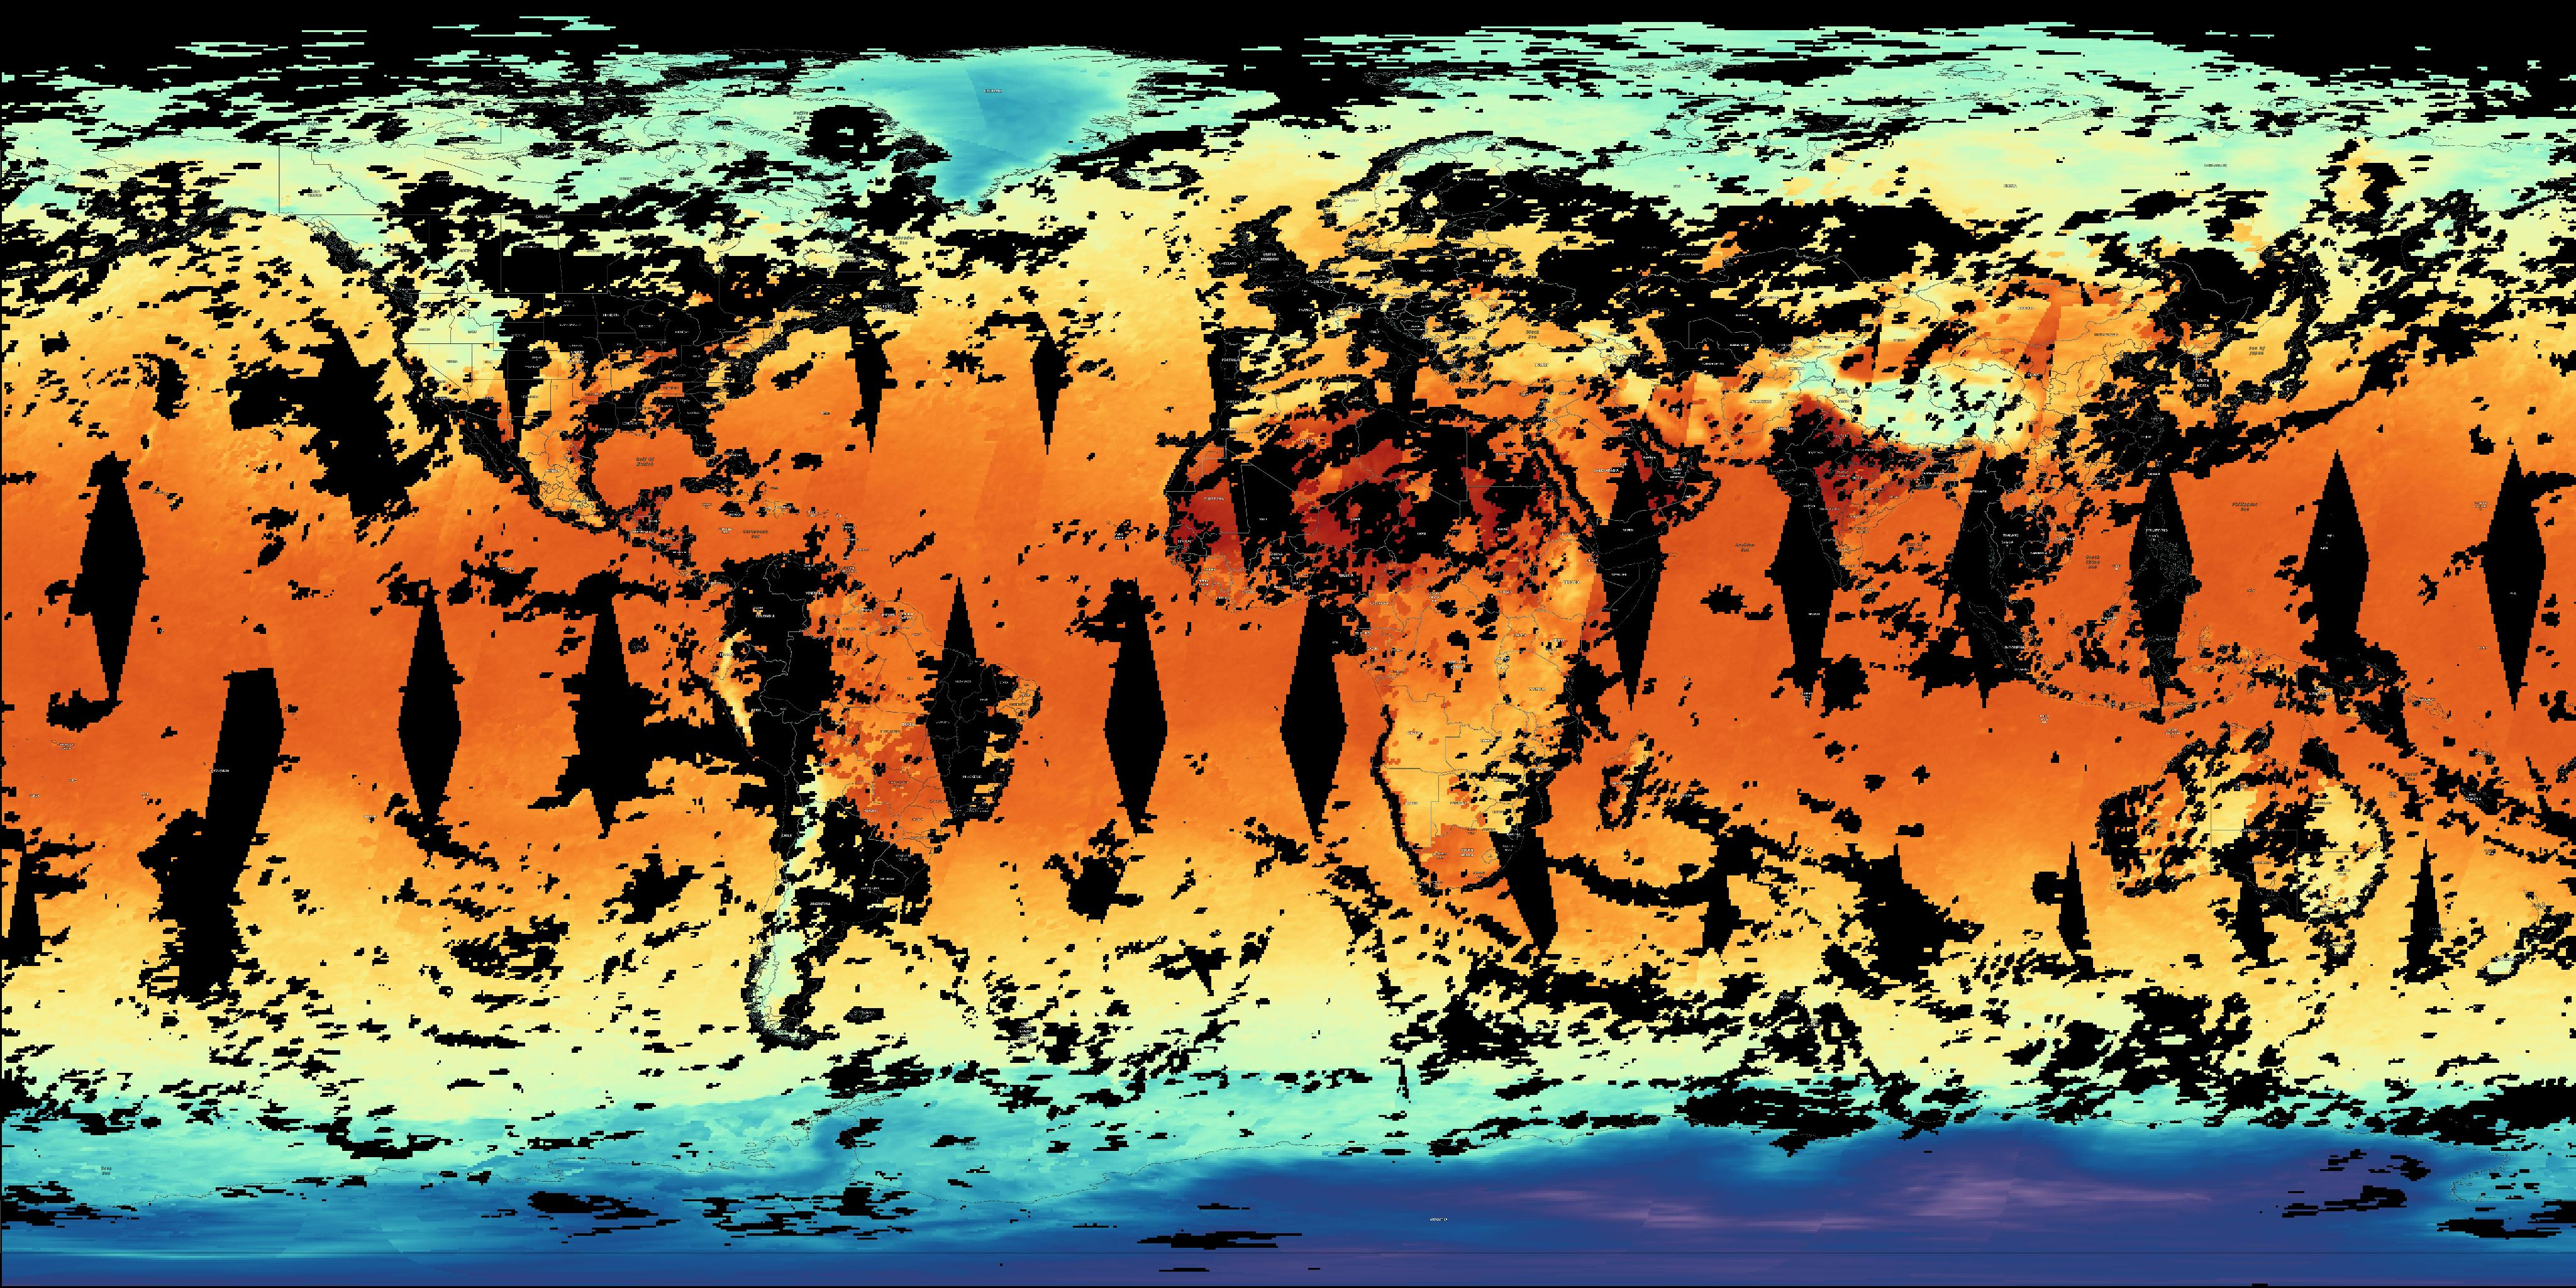
\includegraphics[width=1.0\linewidth]{figures/snapshot_nasa_airs_aqua_2024_05_21T00_00_00Z.jpg}
    \caption{Daytime and nighttime surface air temperature from observations by the AIRS instrument onboard the NASA AQUA satellite. This shows observations recorded through a whole day on the 21\textsuperscript{st} of May 2024. Notice that parts of the globe, especially near the equator have not been observed. This image was produced using NASA Worldview (\url{https://go.nasa.gov/46SaYyJ}).}\label{fig:satellite_image_coverage}
\end{figure}

Forecasting the weather or evolution of any other system is formulated as an initial value problem where past observations are used to predict an unknown future state of the system. A different formulation can be how heat spreads over time in different types of frying pans from known information of the pan's materials, their heat conduction properties, and that the stove gives off constant heat. In general the scenario is predicting the effect (future atmospheric temperature distribution, etc.) of some given causes (current and past weather, etc.). This scenario is termed the forward problem. The inverse problem on the other hand solves for an unknown parameter using other known parameters and observations of the partial solution such as temperature field at the object's surface. Traditional methods used to solve these problems utilized knowledge of the exact equations to numerically solve PDEs. As an example, the Finite Difference Method (FDM) approximates the solution by substituting the partial derivatives with finite differences and manipulating the equation such that the solution can be computed. The inverse problem on the other hand is determination of initial conditions or other parameters from observed state of the system. For example determining the heat source distribution given the temperature distribution at some point in time. One traditional approach to this would have meant solving the forward problem from an initial guess of the parameter and then evaluating some cost function such as how close the predicted solution is to the observed one. As expected, this would require many evaluations of the forward solver. This means that the cost of the solver would be greatly multiplied, emphasizing the importance of an efficient solver.
% TODO: reword this because the explanation of the problem setup for forward and inverse problems is not layed out optimally.
% TODO: perhaps the disadvantage of inverse problem in the paragraph above should be removed and only explanation of the inverse problem setup itself left by itself
% \begin{equation} \label{eq:forward_finite_difference_1}
%     \pdv{f\left(x\right)}{x} \approx \frac{f\left(x+h\right)-f\left(x\right)}{h}
% \end{equation}

Traditional numerical solvers have enjoyed many decades of development due to their long history. There are many general approaches to solve PDEs and many more very specific approaches. Other than FDM, some widely used approaches include Finite Element Methods (FEM), Finite Volume Methods (FVM), Collocation Methods, and Spectral Methods. FEM and FDM are both mesh based approaches, meaning they rely on discretization of the computational domain. There are several challenges associated with this. First, irregular domains such as bio-inspired materials like bone, spider silk, or aggregate materials like gravel pose a challenge due to the complexity of the domain geometry \autocite{gaulSimulationWavePropagation1991,buoniEfficientScalableNumerical2007,jiaModulateStressDistribution2024}. Also, irregular domains which create large deformations or mesh entanglement cause these methods to become ineffective \autocite{chenMeshfreeMethodsProgress2017}. While there are strategies to mitigate this, by definition they are an additional layer of difficulty to the process. Second, multiscale applications where the micro and macro scales are both important require fine meshes such that the small scale structures are adequately simulated. This creates meshes with very large number of points that are very resource intensive \autocite{buoniEfficientScalableNumerical2007}. Third, a single evaluation of traditional mesh-based solvers may not be very costly, however multiple evaluations can add up. This is very apparent in inverse problems where the solver is queried multiple times to solve the forward problem in order to obtain parameter functions. Therefore, in problems where these issues important or resources are limited, mesh-free methods may be preferred. As an example, the spectral method solves PDEs by formulating the solution as a linear combination of global basis functions like the Fourier series. This can be likened to how music combines different sound waves to produce the overall sound. For some function \(s\), the approximation \(s^*\) gets closer to the original with more linear combinations of basis functions. The complex formulation of the Fourier series is presented in \lccref{eq:fourier_series}. With this approach, the approximated function is characterized completely by its coefficients \(c_k\). This fact is exploited by the spectral method to solve differential equations. The solution function can be approximated by finding the mapping between input function coefficients and solution function coefficients. The mapping between a function \(s\) and its derivative \(s^{\prime}\) can be found using the derivative equation from their coefficients leading to \(\hat{s}_k = \hat{s}^{\prime}_k/\left(2\pi ik\right)\). Practically this would be done with a finite number of coefficients (\(k < \infty \)) and the coefficients \(\hat{s}^{\prime}_k\) are obtained using a Discrete Fourier Transform (DFT) algorithm like the Fast Fourier Transform (FFT).
% TODO: Add diagram example for discretization of the domain by FEM/FDM methods
\begin{align}
    s & \approx s^* = \sum_{k} \hat{s}_k e^{2\pi ikx}\label{eq:fourier_series}
\end{align}
This leads us to the fourth challenge with traditional methods which is that they require prior knowledge of analytic forms of PDEs. This is because traditional solvers use the equations to formulate solutions. This makes traditional numerical approaches unsuited to problems where the governing equations are unknown or partially known. These challenges altogether are some of what weather forecasting faces; NWP has the immense task of modeling multiple scales of the Earth's atmosphere while accounting for features of physical systems that are still not fully understood. Many other fields such as epidemiology \autocite{brauerMathematicalModelsEpidemiology2019} and ecology \autocite{holmesPartialDifferentialEquations1994,turchinDoesPopulationEcology2001} also face these challenges. As with many other fields, at some point in time the governing equations of many systems were not known. This has motivated research into alternative methods that do not completely rely on prior knowledge, are mesh free, and fast enough when solving forward problems.

\subsection*{Machine Learning for PDEs}
With the increasing prevalence of machine learning methods and their use in more and more fields, research into their use for scientific computing has taken off in recent years. While statistical modeling has already been widely used in areas such as physical constants, stellar population studies, risk assessments of events such as earthquakes and coronal mass ejections \autocite{berlinerPhysicalStatisticalModeling2003,anselmoComputationalMethodsReentry2005,reinhardtAsteroidRiskAssessment2016,uzanFundamentalConstantsTheir2003,spanosWhereStatisticalModels2006,bernardiStellarPopulationAnalysis2022}, the dominant approach for forward modeling or inverse modeling has remained physics based numerical models. Machine learning has provided an alternative approach to model the solutions of PDEs. In their work, \textcite{aartsNeuralNetworkMethod2001} utilized neural networks to approximate each term of PDEs describing damped and undamped free vibrations and substituting them into the PDEs and associated initial conditions. The network parameters were then optimized to reduce the PDE residual and boundary condition loss using evolutionary algorithms. This approach was taken in order to make machine learning models more transparent which at the time was being pursued because of the high cost of optimizing uncertainties in water management numerical simulators. However, since this method approximates the mapping between coordinates and the values of a function and their derivatives, retraining would be necessary for changes to the function itself. This could become very costly as retraining costs accumulate. A more recent approach that also utilizes soft constrains from PDE residuals is termed physics informed neural network (PINN) \autocite{raissiPhysicsinformedNeuralNetworks2019}. The authors propose a framework that leverages advancements in computing, namely automatic differentiation (AD) techniques made readily available by modern machine learning libraries. In general, PINNs use AD to compute each term of the PDE from the output of the model and this is then substituted into the PDE to in order to compute the residuals and loss from boundary conditions. The network residual and boundary loss are then weighted and summed with the data loss. For a neural network \(\hat{u}\left(\vb{x},t\right)\) approximating the real solution \(u\left(\vb{x},t\right)\), the residual loss for the heat equation in \lccref{eq:heat_equation} is \lccref{eq:heat_pinn_loss}. There are several advantages of incorporating physics knowledge into the model including regularization of the model outputs to be more consistent with physics, faster convergence, and less to no data required depending on whether the network is trained in a manner that is supervised, self-supervised, or a combination of both. One issue with using AD to compute the residual is that the network input needs to be the independent variable (i.e.\ coordinates, time, etc.). This once again means that if one wants to compute a different solution, the network needs to be retrained.
\begin{equation}\label{eq:heat_pinn_loss}
    \mathcal{L}_{PDE}={\left(\pdv{\hat{u}\left(\vb{x},t\right)}{t}-\divergence{\left(\alpha \gradient \hat{u}\left(\vb{x},t\right)\right)}\right)}^2
\end{equation}
\subsection*{Learning PDEs with CNNs}
Other works utilize convolutional neural networks (CNN) to compute the solution from input functions such as forcing terms or initial conditions. This approach generally means discretizing the functions on a grid and using these as training data. One study by \textcite{wangPhysicsinformedDeepLearning2020} predicts turbulent flow using spatial and temporal decomposition and a specialized U-Net, an architecture based on CNNs, to predict the velocity field from the decomposition of the previous velocity field. Part of the loss function is a regularization term for zero divergence in the velocity field to enforce incompressible fluid flow. This term was calculated using finite differences since auto differentiation is not applicable in this situation. Finite differences was also utilized in another CNN based fluid flow upscaling model by \textcite{gaoSuperresolutionDenoisingFluid2021} to compute the residual terms of the steady incompressible Navier-Stokes equation. This model also inferred unknown physical parameters such as boundary conditions. However, this approach would mean the model would need to scale as a quadratic in 2D, cubic in 3D, and much steeper in higher dimensions. Outside fluid dynamics, the combination of specialized CNNs and finite differences or another numerical differentiation method have been used for many other PDEs including Poisson's equation for temperature fields \autocite{zhaoPhysicsinformedConvolutionalNeural2023, gaoPhyGeoNetPhysicsinformedGeometryadaptive2021}, velocity models from seismic data \autocite{mullerDeepPretrainedFWI2023}, and seismic response of structures \autocite{zhangPhysicsguidedConvolutionalNeural2020,niMultiEndPhysicsInformedDeep2022}. While the use of CNNs mean that discretization is implied, solutions of different initial conditions or parameter functions can be computed by inference and no retraining is required. This property is especially useful for many-query problems such as computing gradients for inverse problems.

\subsection*{Operator Learning}
The mapping between discretized functions done by CNNs are related to an alternative approach that starts by viewing PDEs as operators, which are generalized mappings between spaces. One group of familiar operators are functions which maps between spaces of scalar values or vector values. PDEs on the other hand are operators that map between function spaces. A simple example is the derivative. The derivative takes in a function and returns the derivative of said function. In other words it is an operator that maps between the space of all functions to the space of derivatives of those functions. Another way to view operators starts by viewing functions as infinite dimensional vectors. Where elements in the vector are the function's value evaluated at every point in space. The operator can be seen as a vector function mapping between these infinite dimensional vector spaces. Operators are important because a field of research has sprung up around this mathematical concept. Operator learning is the use of machine learning to learn operators using data driven approaches. As an analogy, function regression traditionally has been used to approximate the mapping between input values such as coordinates and output values of functions evaluated at said coordinates. In the case of operator learning, the mapping between function spaces are approximated. The aforementioned approaches using CNNs does this directly using the values of functions at discrete points. There are other approaches like DeepONet that does not require the uniform grid like CNNs \autocite{luLearningNonlinearOperators2021}. This architecture instead uses both input functions and coordinates as inputs. The output is the output function evaluated at the coordinates provided. This architecture is based on an extension for deep learning of the universal operator approximation theory for neural networks first proposed almost three decades ago at the time of writing by \textcite{chenUniversalApproximationNonlinear1995}. The proposed architecture is composed of two subnetworks, where one termed the trunk \(\hat{\vb{T}}\left(\vb{x},t\right)\)learns the latent mapping for coordinates and the other network termed the branch \(\hat{\vb{B}}\left(\vb{f}\right)\) learns the latent mapping for the input function \(f \). The two latent mappings are combined through a dot product to obtain the approximated output function value \(u \left( \vb{x}, t \right)\). This is formulated in \lccref{eq:universal_op_approx_nn}.
\begin{equation}\label{eq:universal_op_approx_nn}
    u\left( \vb{x}, t \right) \approx \hat{G}\left( \vb{f} \right)\left( \vb{x}, t \right) = \hat{\vb{B}}\left( \vb{f} \right) \cdot \hat{\vb{T}}\left( \vb{x}, t \right)
\end{equation}
Fourier Neural Operators (FNO) is an alternative avenue for learning operators by utilizing the fact that functions can be decomposed into linear combinations of basis functions, namely trigonometric basis in this particular case \autocite{li2021fourier}. With this method the input function value is mapped to its corresponding output function value. This is done by first lifting the input function value to a higher dimension using a neural network and this is then passed through blocks composed of a Fourier transform, then a linear transform and filtering of higher modes, and finally the inverse Fourier transform. These blocks are stacked to a desired depth and finally another network projects the outputs to the target dimension. The reason a linear can be used is that differentiation is multiplication in the Fourier domain. One drawback with FNO is the requirement that output functions are not parameterized by coordinates and therefore is implicitly relative to the input function coordinates. To avoid this issue, \textcite{fanaskovSpectralNeuralOperators2023} reframes the problem by directly utilizing the coefficients of Fourier or Chebyshev basis. The model, termed Spectral Neural Operator (SNO) is trained on features of input function coefficients which are computed using Fourier or Chebyshev transforms and labels of output function coefficients using the same transforms. The authors point out one motivation for this approach which is that training neural networks on discretized data may not be ideal because unexpected outputs such as non-smooth interpolation may happen when the network is trained on one grid size and evaluated other grid sizes. With SNO, the interpolation of the function is smooth due to interpolation being done by Fourier basis functions which are sines and cosines for example. In a similar study, \textcite{du2024neural} extends the concept of mapping coefficients by proposing residuals in the spectral domain and leveraging Parseval's Identity to compute the spectral analog to the loss term in PINNs. This allows for self supervised learning in the spectral domain. The same benefits incorporating physics into PINNs also apply here without the pain points introduced by discretized model inputs and outputs. As a whole, operator learning creates an alternative approach that addresses the issue of retraining or recomputing the solution model. In addition, due to its data based approach, even systems with partially or fully unknown governing equations may be simulated.

A persistent challenge with all these approaches is the issue of optimization. While neural networks are modular and expressive which is proven by the universal approximation theorem \autocite{cybenkoApproximationSuperpositionsSigmoidal1989,hornikMultilayerFeedforwardNetworks1989}, their loss function present many local minima meaning it is non-convex. This can be mitigated by using advanced optimization techniques that can find a local minima close enough to the global minima such as Adam \autocite{shresthaReviewDeepLearning2019,soydanerComparisonOptimizationAlgorithms2020}. However, the addition of PDE residuals into the loss function have worsened the highly non-convex loss landscape issue \autocite{rathoreChallengesTrainingPINNs2024,NEURIPS2021_df438e52,basirCriticalInvestigationFailure2022}. These problems range from the disparity in size of boundary and residual loss gradients to the fact that incorporation of residuals and boundary conditions themselves create a much more complex loss landscape. As a result, it is desirable to utilize a different machine learning algorithm that possesses a convex loss landscape. One family of such algorithms are Support Vector Machines (SVM) \autocite{vapnikNatureStatisticalLearning2000}. The appeal of SVMs are the fact that the model is formulated as a quadratic programming problem. This means there are strong guarantees for convergence, generalization, and complexity. Another formulation called Least Squares Support Vector Machines (LSSVM) reformulates the problem as a linear system \autocite{suykensLeastSquaresSupport2005}. This leads to an easier problem that can be computed faster by well established algorithms like the many implementations of least squares solvers. Another advantage of the linear formulation is that this can be easily parallelized to exploit hardware like graphics processing units more widely known as GPUs in contrast to the commonly used Sequential Minimal Optimization (SMO) used for SVMs with quadratic objective functions.

The advantageous properties of SVM based methods have attracted research into their use for solving PDEs. An early work using SVMs to solve PDEs by \textcite{youxiwuSVMSolvingForward2005} introduced a method for solving the forward problem of Electro-Impedance Tomography. This work solved for the mathematical model of EIT which is given by Maxwell's equations by modeling the trial function as using an \(\epsilon \)-SVR model. Another approach much more similar to PINNs was presented by \textcite{mehrkanoonLearningSolutionsPartial2015}. The residual and initial/boundary conditions are imposed as equality constraints on an LS-SVM objective function. A different study by \textcite{leakeAnalyticallyEmbeddingDifferential2019}, the incorporation of physics into the model is done slightly differently by utilizing the theory of functional connections to directly embed constraints into the solution. This means that the proposed method would satisfy the boundary condition exactly. However, the authors point out that for PDEs in higher dimensions deriving and implementing this method can become cumbersome. These approaches, however, do not learn the PDE operator itself. Meaning they are also not practical for many-query problems.

\subsubsection*{Operator Learning for Weather Forecasting}
In terms of weather forecasting, operator learning has been applied in terms of initial value problems. This problem formulation is reminiscent of time series prediction problems widely found in machine learning research. Researchers \textcite{kurthFourCastNetAcceleratingGlobal2023} developed FourCastNet which utilized Adaptive Fourier Neural Operator (AFNO), a transformer based model containing the previously mentioned FNO computational blocks by \textcite{li2021fourier}. This model was then able to be trained in a massively parallel manner. In a comparison with a traditional model called the Integrated Forecasting System from the European Center for Medium Range Weather Forecasts (ECMWF), FourCastNet is faster and much more efficient in terms of inference time, resulting in about 80,000 times speed up for a 100-member ensemble forecast. This is while performing much better than a previous deep learning approach. In another study, \textcite{bonevSphericalFourierNeural2023} proposed a variation on neural operators called Spherical Fourier Neural Operator (SFNO) which exploited the spherical nature of global forecasting by using Spherical Harmonic Transform (SHT) in place of Fourier Transform. This model when compared to AFNO and FNO, produced no visible artifacts in autoregressive rollouts for long range forecasting. In terms of forecasting, the model shows outcomes that matches the IFS which is a big leap forward in parity for traditional and machine learning based methods.

% Bagian ini mendeskripsikan gambaran umum, konteks, dan posisi penelitian TA dalam konstelasi perkembangan pengetahuan yang telah dicapai. Penjelasan yang dituliskan menjadi penting karena dengan landasan yang kuat, maka pekerjaan penelitian dapat terarah dilakukan. Hal ini lebih spesifik dan tegas disampaikan pada sub-sub bab berikutnya.

% Beberapa pustaka utama yang berperan dominan dapat disampaikan di sini untuk memberi gambaran tentang letak penelitian TA dalam konstelasi keilmuan yang dicapai. Hasil-hasil dari pustaka terbaru dapat menopang Latar Belakang ini menjadi lebih kuat.

% Sangat wajar apabila isi sub bab setelah Latar Belakang ini mengalami penyesuaian saat sejumlah hasil penelitian sudah diperoleh dan dianalisis. Pada dasarnya, hal ini dimungkinkan apabila ada penyesuaian kecil, karena fokus penelitian sejatinya sudah jelas sedari awal, namun hasil-hasil yang diperoleh dapat memperbaharui beberapa butir isi sub bab. Oleh karena itu, finalisasi isi Pendahuluan ini biasanya dilakukan menjelang akhir pembuatan laporan penelitian yang dituangkan dalam buku TA.


\section{Problem Statement}\label{sec:problem_statement}
\noindent The problems this work sets out to solve based on \lccref{sec:background} are:
\begin{enumerate}
    \item What is the formulation a computational model for operator regression and therefore solving PDEs in the spectral domain using support vector machines?
    \item Can the model learn the relationships represented by PDEs? And how does it perform on different problems?
    \item How can one interpret the learned model?
\end{enumerate}

% Bagian ini menjadi salah satu bagian penting dalam Pendahuluan. Setelah paparan Latar Belakang, maka masalah yang diangkat pada pekerjaan penelitian perlu dirumuskan dengan baik. Perumusan ini sebaiknya dibahasakan tidak dalam bentuk kalimat pertanyaan, melainkan kalimat aktif, dan dapat memuat lebih dari satu rumusan.

% Sejalan dengan ini, setiap masalah yang diangkat selalu memiliki batas. Ada batasan, asumsi, atau kriteria yang menjadi pembatas atas masalah yang diangkat dalam penelitian TA, sehingga arah penelitian dapat fokus. Batasan ini perlu dituliskan secara tegas, dan dapat saja memuat lebih dari satu.


\section{Aims}\label{sec:aims}
\noindent Based on the stated problems in \lccref{sec:problem_statement}, this study aims to acomplish the following:
\begin{enumerate}
    \item The design and implementation of a computational model that maps coefficients in the spectral domain using Least Squares Support Vector Regression (LSSVR).
    \item Proof of the model's learning ability using three different problems.
    \item Interpretation the model results and why some predictions turn out the way they do.
\end{enumerate}
% Bagian ini secara tegas menuliskan tujuan pekerjaan penelitian TA, yang dapat memuat lebih dari satu. Pemilihan kata kerja pada Tujuan ini sangat penting karena menggambarkan arah fokus dari jalinan upaya yang dilakukan.

\section{Contribution}
\noindent In achieving the aims of this study the following contributions are made:
\begin{enumerate}
    \item A novel use LSSVR which has a convex objective to learn solution operators of partial differential equations and operators in general.
    \item Interpretation of machine learning model trained on operator data.
\end{enumerate}

\section{Limitations}
\noindent This work is limited to the following:
\begin{enumerate}
    \item Functions the model works with are only continuous functions.
    \item The basis functions are limited to Fourier basis.
    \item Modeled fields are compact or dense meaning not sparse. Sparse observations or other data are assimilated using other methods.
\end{enumerate}

\section{Sistematika Penulisan}
% \noindent Bagian ini adalah penutup Bab I yang menyampaikan  secara ringkas isi setiap  bab. Karena pembaca sudah sampai akhir Bab I, yang  berarti  sudah  mengetahui isinya, maka tidak perlu ditulis lagi rincian Bab I. Sebaiknya langsung dituliskan secara ringkas isi rincian bab-bab selanjutnya, misalnya, \textit{Setelah Pendahuluan pada Bab I ini, Bab II akan mengulas tentang ...}

% Apabila diperlukan, dapat dituliskan konvensi khusus yang digunakan pada penulisan naskah buku TA ini, misalnya tanda titik menggantikan tanda desimal karena alasan kemudahan dan kejelasan dalam formulasi matematika.
% !TEX root = ./skripsi.tex
\chapter{KAJIAN PUSTAKA}

\noindent Bab ini mengulas secara rinci konsep-konsep dasar yang berkaitan dengn pekerjaan penelitian TA dan deskripsi studi pustaka yang dilakukan. Judul bab tidak harus seperti yang dituliskan, melainkan dapat lebih fleksibel yang mencerminkan isi paparan pada bab ini. Demikian halnya dengan judul sub bab.

\section{Fourier Transform and Series}
\noindent

Complex numbers are numbers consisting of real and imaginary components. Complex numbers are written as in \lccref{eq:complex_number} with \(a \) and \(b \) being the real and imaginary components respectively. The imaginary component is multiplied by the imaginary unit \(i=\sqrt{-1}\).
\begin{align}
  c = a + bi \label{eq:complex_number} \\
\end{align}

\section{Least Squares Support Vector Machine}
\noindent An arguably fundamental model widely used whether in pedagogical settings or otherwise is the support vector machine. It dates back to works by Vapnik \& Lerner in 1963 (Recognition of Patterns with help of Generalized Portraits) and V. N. Vapnik \& A. Ya. Chervonenkis in 1964 (A note on one class of perceptrons/On a perceptron class). As the development on SVM continued, what originally was a model for classification of separable data generalized to regression tasks as well Vapnik (2000 The Nature of Statistical Learning Theory).
\subsection{Disadvantages}
However, the main disadvantage of LSSVMs are the fact that they do not have the sparse property of SVMs which can leave performance on the table. A simple mitigation can be done by filtering training samples with small absolute values of lagrangian multipliers \autocite{haifengwangComparisonSVMLSSVM2005}.

To derive the least squares support vector regression (J.A. Suykens LSSVM Book) model we start with the linear expression:

\begin{equation}
  y=W^{\intercal}\vb{x}+b
\end{equation}

\begin{equation}
  \min_{W,e} J(W,e) = \frac{1}{2}W^{\intercal}W + C\frac{1}{2}\sum_{k=1}^{n}e_{k}
\end{equation}

Such that
\begin{equation}
  y_{k}=W^{\intercal}\vb{x}_{k}+b+e_{k} \qquad k=1,\dots,n
\end{equation}

\begin{equation}
  L(W,b,e;\vb{\alpha}) = \frac{1}{2}W^{\intercal}W + C\frac{1}{2}\sum_{k=1}^{n}e_{k} + \sum_{k=1}^{n}\alpha_{k} \left(W^{\intercal}\vb{x}_{k}+b+e_{k} - y_{k} \right)
\end{equation}

Derive the KKT system
\begin{equation}
  \begin{split}
    \pdv{L}{W} = 0 \rightarrow & W = \sum_{k=1}^{n}\alpha_{k}x_{k} \\
    \pdv{L}{b} = 0 \rightarrow & \sum_{k=1}^{n}\alpha_{k} = 0 \\
    \pdv{L}{e_{k}} = 0 \rightarrow & \alpha_{k} = C e_{k} & \qquad k=1,\dots,n\\
    \pdv{L}{\alpha_{k}} = 0 \rightarrow & W^{\intercal}\vb{x}_{k}+b+e_{k} - y_{k} = 0 & \qquad k=1,\dots,n\\
  \end{split}
\end{equation}

After eliminating $W$ and $\vb*{e}$, with $\vb{1}_{n} = \langle 1,\dots,1\rangle$, $\vb{y} = \lbrack y_1, \dots, y_n \rbrack $, and ${\alpha} = \lbrack \alpha_1, \dots, \alpha_n \rbrack $ the solution is as follows in block matrix notation
\begin{equation} \label{eq:lssvr_solution}
  \begin{bmatrix}
    0          & \vb{1}_{n}^{\intercal} \\
    \vb{1}_{n} & \Omega + \frac{I}{C}
  \end{bmatrix}
  \begin{bmatrix}
    b           \\
    \vb{\alpha} \\
  \end{bmatrix}
  =
  \begin{bmatrix}
    0      \\
    \vb{y} \\
  \end{bmatrix}
\end{equation}

The solution in \cref{eq:lssvr_solution}

\begin{algorithm}[H]
  \caption{LSSVR Training}\label{alg:lssvr_training}
  \begin{algorithmic}[1]
    \Procedure{SolveLSSVR}{$\vb{X}, \vb{y}, \gamma $}
    \State{\(\Omega \gets [[]]\)}
    \Comment{Construct matrix of inner products in high dimensional space}

    \For{\(k=0 \to n\)}
    \For{\(l=0 \to n\)}
    \State{\(\Omega_{k,l}\gets K(\vb{X}_k,\vb{X}_l)\)}
    \EndFor{}
    \EndFor{}
    \State{\(\vb{H} \gets \Omega + \frac{\vb{I}}{\gamma}\)}
    % \State $\vb{1} \gets [1,1,...,1]$
    \State{\(\vb{A} \gets [[]]\)}
    \Comment{Construct left-hand side matrix}
    \State{\(\vb{A}_{0,0} \gets 0\)}
    \For{\(k=0 \to n\)}
    \State{\(\vb{A}_{k+1,0} \gets 1\)}
    \State{\(\vb{A}_{0,k+1} \gets 1\)}
    \EndFor{}
    \For{\(k=0 \to n\)}
    \For{\(l=0 \to n\)}
    \State{\(\vb{A}_{k+1,l+1} \gets \vb{H}_{k,l}\)}
    \EndFor{}
    \EndFor{}
    \State{\(\vb{B}\gets []\)}
    \Comment{Construct left-hand side of the equation}
    \State{\(\vb{B}_0 \gets 0\)}
    \For{\(k=0 \to n\)}
    \State{\(\vb{B}_{k+1} \gets \vb{y}_{k}\)}
    \EndFor{}
    \State{\(\vb{A}^{\dagger} \gets pseudoInverse(\vb{A})\)}
    \Comment{Compute solution using pseudo inverse}
    \State{\(\vb{S} \gets \vb{A}^{\dagger}\vb{B}\)}
    \State{\(b \gets \vb{S}_{0}\)}
    \For{\(k=0 \to n\)}
    \State{\(\vb{\alpha}_{k} \gets \vb{S}_{k+1}\)}
    \EndFor{}
    \State{\textbf{return}\(\vb{\alpha}, b\)}
    \EndProcedure{}
  \end{algorithmic}
\end{algorithm}

The basic pseudocode from the LSSVM Equation for function regression is defined in \lccref{alg:lssvr_training} for a training set of length $n$, features $\vb{X}$, and labels $\vb{y}$. Training the LSSVM means computing the values of langrange multipliers $\vb{\alpha}$ and bias $b$. $K$ is the kernel function used to compute the inner products in high dimensional space, here we assume the RBF kernel. $\vb{A}$ is a matrix of size $n+1$ by $n+1$. $\vb{H}$ is a matrix of size $n$ by $n$. $\vb{I}$ is the identity. $\vb{B}$ is a vector of size $n+1$. $\vb{S}$ is a vector of size $n+1$.

After training the model can be used for prediction of unseen features. The pseudocode for prediction is shown in \lccref{alg:lssvr_prediction} for prediction features $\vb{U}$ with \(p \) samples. The trained model uses the training features themselves $\vb{X}$ with \(n \) samples, the learned multipliers of training points $\vb{\alpha}$, and the bias $b$.

\begin{algorithm}[H]
  \caption{LSSVR Prediction}\label{alg:lssvr_prediction}
  \begin{algorithmic}[1]
    \Require $\vb{U}, \vb{\alpha}, \vb{X}, b$
    \Ensure $\vb{v}$
    \State $\Omega \gets [[]]$ \Comment{Construct matrix of inner products in high dimensional space}

    \For{$k=0 \to p$}
    \For{$l=0 \to n$}
    \State$\Omega_{k,l}\gets K(\vb{U}_{k},\vb{X}_l)$
    \EndFor
    \EndFor
    \State $\vb{v} \gets \Omega\vb{\alpha} + \vb{1}_{m}b$
  \end{algorithmic}
\end{algorithm}

In this exmple we will be using the function $2x^2+4$. The values of this function can be seen in Table \ref{table:1}.

\begin{table}[H]
  \centering
  \begin{tabular}{@{}lll@{}}
    \toprule
    No & x       & y       \\ \midrule
    1  & 0.0     & 4.0     \\
    2  & 0.33... & 4.22... \\
    3  & 0.66... & 4.88... \\
    4  & 1.0     & 6.0     \\
    \bottomrule
  \end{tabular}
  \caption{Example data of function $2x^2+4$} \label{table:1}
\end{table}
For $\Omega_{i,j}=K(x_i,x_j)=exp \left(-\frac{\norm*{x_i-x_j}^2}{2\sigma^2}\right)$

For example, with $\sigma=1$, $x_i=0.0$, \& $x_j = 0.33\dots$
\begin{equation}
  \begin{split}
    K(0.0,0.33) & = exp\left(-\frac{\norm*{0.0-0.33}^2}{2(1)^2}\right) \\
    & = exp\left(-\frac{0.33^2}{2}\right) \\
    & = 0.9460
  \end{split}
\end{equation}

\begin{equation}
  \Omega\gets
  \begin{bmatrix}
    1.0000 & 0.9460 & 0.8007 & 0.6065 \\
    0.9460 & 1.0000 & 0.9460 & 0.8007 \\
    0.8007 & 0.9460 & 1.0000 & 0.9460 \\
    0.6065 & 0.8007 & 0.9460 & 1.0000 \\
  \end{bmatrix}
\end{equation}

\begin{equation}
  \vb{I}\frac{1}{\gamma}\to\vb{I}\frac{1}{5}\to
  \begin{bmatrix}
    0.2000 & 0.0000 & 0.0000 & 0.0000 \\
    0.0000 & 0.2000 & 0.0000 & 0.0000 \\
    0.0000 & 0.0000 & 0.2000 & 0.0000 \\
    0.0000 & 0.0000 & 0.0000 & 0.2000
  \end{bmatrix}
\end{equation}

\begin{equation}
  \Omega+\vb{I}\frac{1}{5}\to H\to
  \begin{bmatrix}
    1.2000 & 0.9460 & 0.8007 & 0.6065 \\
    0.9460 & 1.2000 & 0.9460 & 0.8007 \\
    0.8007 & 0.9460 & 1.2000 & 0.9460 \\
    0.6065 & 0.8007 & 0.9460 & 1.2000 \\
  \end{bmatrix}
\end{equation}

\begin{equation}
  A\to
  \begin{bmatrix}
    0.0000 & 1.0000 & 1.0000 & 1.0000 & 1.0000 \\
    1.0000 & 1.2000 & 0.9460 & 0.8007 & 0.6065 \\
    1.0000 & 0.9460 & 1.2000 & 0.9460 & 0.8007 \\
    1.0000 & 0.8007 & 0.9460 & 1.2000 & 0.9460 \\
    1.0000 & 0.6065 & 0.8007 & 0.9460 & 1.2000 \\
  \end{bmatrix}
\end{equation}

\begin{equation}
  B\to
  \begin{bmatrix}
    0.0000 \\
    4.0000 \\
    4.2222 \\
    4.8889 \\
    6.0000 \\
  \end{bmatrix}
\end{equation}

\begin{equation}
  A^{\dag}\to
  \begin{bmatrix}
    -0.8994 & 0.4348  & 0.0652  & 0.0652  & 0.4348  \\
    0.4348  & 2.0686  & -1.6490 & -0.5292 & 0.1096  \\
    0.0652  & -1.6490 & 3.3774  & -1.1992 & -0.5292 \\
    0.0652  & -0.5292 & -1.1992 & 3.3774  & -1.6490 \\
    0.4348  & 0.1096  & -0.5292 & -1.6490 & 2.0686  \\
  \end{bmatrix}
\end{equation}

\begin{equation}
  A^{\dag}B\to S\to
  \begin{bmatrix}
    4.9421  \\
    -0.6177 \\
    -1.3737 \\
    -0.5625 \\
    2.5538  \\
  \end{bmatrix}
\end{equation}

\begin{equation}
  b\to 4.9421
\end{equation}

\begin{equation}
  \alpha \to
  \begin{bmatrix}
    -0.6177 \\
    -1.3737 \\
    -0.5625 \\
    2.5538  \\
  \end{bmatrix}
\end{equation}

Prediction
\begin{equation}
  U\to
  \begin{bmatrix}
    0.3 \\
    0.2 \\
    0.5
  \end{bmatrix}
\end{equation}

\begin{equation}
  \Omega\to
  \begin{bmatrix}
    0.9560 & 0.9994 & 0.9350 & 0.7827 \\
    0.9802 & 0.9912 & 0.8968 & 0.7261 \\
    0.8825 & 0.9862 & 0.9862 & 0.8825 \\
  \end{bmatrix}
\end{equation}

\begin{equation}
  \Omega\alpha\to
  \begin{bmatrix}
    -0.4904 \\
    -0.6170 \\
    -0.2008 \\
  \end{bmatrix}
\end{equation}

\begin{equation}
  \Omega\alpha+b\vb{1}_{m}\to v\to
  \begin{bmatrix}
    4.4516 \\
    4.3251 \\
    4.7413 \\
  \end{bmatrix}
\end{equation}
Where $\vb{1}_{m}$ is a vector of 1s with the length of $U$.

\section{Sub Bab B}
\noindent Suatu penelitian tidak dapat lepas dari capaian pengetahuan dan pemahaman yang sudah dipublikasikan. Deskripsi tentang capaian ini menjadi penting karena selain menunjukkan tingkat pemahaman mahasiswa, juga mengetahui tempat pekerjaan penelitian TA dalam konstelasi capaian tersebut. Studi pustaka dan paparan hasilnya dapat memperkaya wawasan tentang topik yang diangkat pada penelitian TA.

\section{Membuat Persamaan}
\noindent Secara prinsip, suatu persamaan menyatu dalam kalimat. Letak persamaan dapat berada di awal, tengah, atau akhir kalimat. Dengan demikian, pada akhir persamaan harus diberikan tanda baca, misalnya koma, titik koma, atau titik, yang menekankan kehadiran persamaan dalam kalimat. Tidak semua persamaan harus diberi nomor. Persamaan yang dirujuk pada naskah TA saja yang harus diberi nomor. Kode awal penomoran ini adalah nomor urut bab, termasuk untuk persamaan pada Lampiran, dengan urutan alfabet kapital.

Setiap notasi harus unik atau tunggal, sehingga arti setiap notasi adalah unik atau tunggal juga. Arti satu notasi harus dituliskan segera ketika notasi tersebut muncul, dan tidak diulang lagi setelahnya.

\subsection{Contoh Persamaan Sederhana}
Persamaan (\ref{II.1}) mendeskripsikan dinamika fungsi gelombang $\psi(\vec{r},t)$ di bawah pengaruh potensial $V(\vec{r})$ dan dituliskan sebagai berikut:
\begin{equation}\label{II.1}
  i\hslash\frac{\partial \psi}{\partial t} = -\frac{\hslash^2}{2 m}\Vec{\nabla}^2 \psi + V(\vec{r})\psi,
\end{equation}
dengan $m$ adalah massa partikel dan $\hslash$ merupakan konstanta Planck tereduksi.

Di akhir persamaan (\ref{II.1}) diberi koma karena berada ditengah kalimat. Untuk merujuk ke persamaan yang telah ditulis, gunakan perintah \verb|\ref{}|.

Untuk menuliskan beberapa set persamaan yang masih terhubung, gunakan \verb|\subequations{}|. Misal kita punya persamaan diferensial terkopel, kita bisa tuliskan
\begin{subequations}
  \begin{align}
    \frac{dy}{dt} & = -x , \\
    \frac{dx}{dt} & = -y .
  \end{align}
\end{subequations}
Kalau perlu matriks, kita bisa tulis seperti berikut.
\begin{equation}
  \sigma_x =
  \begin{pmatrix}
    0 & 1 \\
    1 & 0
  \end{pmatrix},\quad
  \sigma_y =
  \begin{pmatrix}
    0 & -i \\
    i & 0
  \end{pmatrix}, \quad
  \sigma_z =
  \begin{pmatrix}
    1 & 0  \\
    0 & -1
  \end{pmatrix}
\end{equation}


\section{Referensi dan Citation}
% \noindent Sitasi dapat dimasukkan ke dalam Tugas Akhir seperti ini \cite{Fujita1996}. Untuk sitasi dengan beberapa sumber, dapat dituliskan juga \cite{hohen1964,Kim2006}. Atau untuk tiga sumber berarti \cite{kongkanand2006,kresse1999,Leibb1993}.

% !TEX root = ./skripsi.tex
\chapter{RESEARCH METHODOLOGY}\label{sec:research_methodology}

% Secara umum, metode penelitian yang digunakan pada pekerjaan penelitian disampaikan pada bab ini. Judul bab tidak harus seperti yang dituliskan. Dalam kata lain bisa diubah sesuai kebutuhan.

\section{Research Design}
\noindent This study is carried out under the framework of a research design. In this section, this design will be laid out and explained. The design includes the process from the beginning to the end of the overall study. The research design is visually depicted in \lccref{fig:research_design_diagram}.

\begin{figure}[H]
      \centering
      \tikzfig{figures/research_design_diagram}
      \caption{Research design diagram}\label{fig:research_design_diagram}
\end{figure}

The study is carried out in 9 main phases. Each phase has a specific aim to accomplish such that the subsequent phases are able to proceed. Each phase is explained as follows:
\begin{numdesc}
      \item[Problem Specification]
      In this phase, relevant literature of related works and other supporting materials will be reviewed to lay the groundwork of this study. Specifically, the literature review will encompass partial differential equations and their real world associations, traditional methods employed to solve them, systems with partially known or unknown governing equations, machine learning approaches to the problem, least-squares support vector machines, performance metrics and tools that will be used such as the PyTorch library.

      \item[Design of Computational Model]
      This phase of the study is allocated to the design of the computational model based on the literature that has been reviewed. The design of the overall process includes data retrieval, preprocessing, and the core spectral regression model itself.

      \item[Implementation of Computational Model]
      After the computational model design is completed, the model is implemented in the Python Language using the PyTorch library as a core component. Implementation of the computational model is done using an iterative software development model. This development model was chosen due to its adaptability to unexpected challenges which is necessary because of the challenges and unknowns with developing a novel method.

      \item[Planning of Experimental Scenarios]
      To properly gauge the performance of the proposed method at approximating operators, specifically the solution operator of partial differential equations, experimental scenarios are developed in this phase. Specifically, the scenarios serves three goals which are proof of concept or validation that the method is able to learn operators, a case study of a more complex system with real world data, and a using the model as a surrogate. Together, these experimental scenarios determine the applicability of the model to the problem. In addition, the model will be compared to a baseline model in order to put into context the proposed model's performance. In addition, kernel-input correlation matrices and input-Lagrangian multiplier inner product matrix will also be computed.

      \item[Data Generation and Retrieval]
      This phase of the study is tied to the experimental scenarios that have been developed. After determination of the scenario specifics, the data that will be used for training, validation, and testing of the model in each scenario will be either generated or retrieved from an external source. In addition, in each scenario the hyperparameters of the model will be determined using Bayesian optimization as an alternative to the traditional grid search method.

      \item[Data Preprocessing]
      The next phase after data generation or retrieval is preprocessing. This is a crucial step in allowing the core LSSVR to learn the mappings in spectral space. In order to do this, the data will need to be reshaped, and important features selected for. Finally, inputs to the LSSVR will need to be normalized or scaled such that the LSSVR model can much more easily learn the data.

      \item[Experiments]
      This phase of the study executes the experimental scenarios that was determined previously. The preprocessed data will be used in accordance to the preplanned scenarios.

      \item[Analysis and Discussion]
      The final phase of the study is the analysis and discussion of the results. Analysis of each experimental scenario will assess the extent of the model's capabilities. Another component of the analysis is interpretation the trained model and how it comes to the predictions that it makes. The discussion will also touch on the hyperparameter optimization and comparisons with the baseline model. This will show how the model performs differently compared to the baseline.
\end{numdesc}

\section{Literature Study Method}
\noindent As a basis for this study, information surrounding the topic is collected from literature sources such as books, journal articles, and other academic works like dissertations. The tools that are used to find these sources include Google Scholar and Google Search. The search terms used start with two terms which are partial differential equations and machine learning. Based on reading the most relevant literature, further search terms are created from variants of previous search terms combined with terms from literature that has been found.

\section{Data Generation and Retrieval Method}
\noindent Data to be used in this study are acquired in two different ways. The first method is data generation. This is motivated by the fact that some partial differential equations do not have much open and accessible real world data available. As such the systems are simulated using the equations themselves. In simple scenarios like computing the antiderivative \(u\) of some function \(f \), this can be done by randomly generating \(u\) and then taking their derivatives to compute \(f\). The random function generation itself is done by generating random coefficients for basis functions like the Fourier series. Once all functions are generated, random noise is added to ensure that the model is also robust towards inexact measurements. A diagram illustrating the process is shown in \lccref{fig:data_generation_diagram}.

\begin{figure}[H]
      \centering
      \begin{adjustbox}{max width=\textwidth}
            \tikzfig{figures/data_generation_diagram}
      \end{adjustbox}
      \caption{Data generation diagram}\label{fig:data_generation_diagram}
\end{figure}

Data retrieval is the other option which in this case is used to retrieve data for weather prediction. Based on the scenario the data is to be used for, relevant subsets of the dataset is retrieved to a working machine. This study specifically uses a dataset provided by the European Center for Medium Range Weather Forecast (ECMWF) named ERA5 hourly data on single levels from 1940 to present \autocite{c3sERA5HourlyData2018}. The first step is selecting a geographical area to study, time period, NetCDF4 data format, and variables such as temperature at 2 meters above the surface. Then the second step is specifications are then used to request the data through the climate data store application programming interface. The downloaded data is then parsed using the Xarray library and preprocessed.

\section{Computational Model Implementation Method}\label{sec:development_method}
\noindent Implementation of the computational model follows an iterative development model. This model basically consists of repeated cycles or iterations of software development. Each cycle is loosely based on the waterfall development model, namely the processes of requirement gathering, analysis \& design, implementation, and testing. This iterative property is crucial for this study because all the requirements cannot be known beforehand. This model minimizes the risk in developing complex software with partially known initial requirements. A diagram of the model can be seen in \lccref{fig:iterative_development_diagram}.

\begin{figure}[H]
      \centering
      \begin{adjustbox}{max width=\textwidth}
            \tikzfig{figures/iterative_development_diagram}
      \end{adjustbox}
      \caption{Iterative development model}\label{fig:iterative_development_diagram}
\end{figure}

This development model was adapted from \textcite{bittnerManagingIterativeSoftware2006}. Each process in the model is explained as follows:
\begin{numdesc}
      \item[Initial Planning]
      The first process of the iterative development model sets up the parameters for the iterative development. These parameters are the broad scope of the project and initial requirements such as core components like LSSVR\@. The initial requirements are crucial in guiding the rest of the development as more requirements are gathered. The initial planning also determines technical choices like tooling and choice of language. The planning process also includes a rough architecture based in initial requirements.

      \item[Requirements]
      This process separates out the backlog of requirements into those that will be worked on in the current iteration. These requirements ideally share some functionality in order to allow the same context to be retained within the iteration which reduces the burden of context switching.

      \item[Analysis and Design]
      This process an analysis of the requirements of the current iteration is performed. This involves determining the constraints and goals for each requirement. Constraints also need to consider previous iterations such that the requirements can be fulfilled effectively and efficiently without regressing progress that has been made such as breaking existing functionality. From this analysis, the design is updated so that the requirement can be fulfilled. The design itself informs how the code should be structured. The interfaces used in the code are also specified.

      \item[Implementation]
      The implementation process applies the design that has been produced. In addition to implementing the program, this process also implements tests which validate and verify the produced code. In the case of complex pieces of the design, an approach of creating tests and assertions first is taken. This way, the code can be run quickly and fail immediately to allow a quicker convergence on the intended functionality.

      \item[Testing and Evaluation]
      Once the design is implemented, tests that have been created are run. Each feature is tested in an integrated manner to expedite the process while still providing enough confidence in the software. The results of the testing process are evaluated and any failed tests are resolved whether by reimplementation or reassessment of the correctness of the tests. Any missing functionality or feature discovered during evaluation are added to the backlog of requirements.

      \item[Release]
      After an iteration, the current version of the software is released. The iterative nature of this development model necessitates the use of a versioning system. As such each release can be identified by a version number loosely based on semantic versioning \autocite{preston-wernerSemanticVersioning2002023}. This version numbering system consists of major number that indicates breaking changes, minor numbers which indicate features and non-breaking changes, and lastly patch numbers are used for fixes. A version number is read as \verb|MAJOR.MINOR.PATCH|. During active development, only major version 0 will be used to prevent too many major versions. The released software is hosted in its own GitHub repository at \url{https://github.com/nidduzzi/SpectralSVR}.

\end{numdesc}

\section{Research Tools}
\noindent The tools that are used in this study can be categorized into hardware and software. The following are hardware that are used in this study:
\begin{itemize}
      \item Kaggle CPU Kernel~\autocite{GettingStartedKaggle}
            \begin{itemize}
                  \item 4 Cores Intel Xeon
                  \item 30 Gigabytes RAM
                  \item 20 Gigabytes Working storage
            \end{itemize}
      \item Kaggle GPU Kernel~\autocite{GettingStartedKaggle}
            \begin{itemize}
                  \item 4 Cores Intel Xeon
                  \item 29 Gigabytes RAM
                  \item 1 Nvidia P100 GPU
                  \item 20 Gigabytes Working storage
            \end{itemize}
      \item Personal Computer
            \begin{itemize}
                  \item Intel i5{-}8300H
                  \item 16 Gigabytes RAM
                  \item Nvidia GeForce GTX 1060 Mobile
                  \item 1.5 Terabytes Storage
            \end{itemize}
\end{itemize}
The software tools used in this study are the following:
\begin{itemize}
      \item Python
      \item Jupyter Notebook
      \item Git
      \item Poetry Python package manager
      \item Web Browser
      \item \LaTeX{}
\end{itemize}

% !TEX root = ./skripsi.tex
\chapter{RESULTS AND DISCUSSION}\label{sec:results_and_discussion}
\noindent This chapter is organized into five sections which are the results of data generation, data retrieval, design of computational model, implementation of computational model, experimental scenarios, and the experiments themselves.

\section{Data Generation}\label{sec:data_generation}
\noindent This study uses two data acquisition approaches. The first approach which is discussed in this section is data generation. This process involves manufacturing data randomly in such a way that they obey the PDEs to be modeled. The generated data consists of features and labels. These features and labels in the context of PDEs are parameters and the solution of the PDEs, respectively. The PDEs enforce a relationship between parameters and the solution. This relationship is implicitly encoded into the features and labels, which is what machine learning models can learn. Because the solution and parameters to PDEs are functions and there are many kinds with different properties, generating all the different kinds of functions is a difficult task. This is why this study focuses on Fourier functions. This means that out of the space of all functions \(F \) which include categories such as polynomials \(f\left(x\right)=a_{n}x^n+\cdots+a_1x+a_0\) where \(f\in F\), and \(a_n\) are constants; we only consider the subset of functions \(U \subset F\) which are of the form \(u\left(x\right)=\sum_{k}^{m}c_k e^{2\pi i k \frac{x}{P}}\).

Using the subset of Fourier functions has several benefits which has motivated the choice. First these functions are characterized purely by their coefficients \(c_k\), meaning there is no need to store discretized values which potentially saves space and computation. The second benefit is that other functions such as polynomials can be approximated by them using the Fourier transform. This means that despite limiting the set of functions to Fourier functions, the behavior of PDEs with other sets of functions can be approximated to a certain extent. The final benefit is the mature ecosystem around these functions which include fast algorithms for the Fourier transform and even numerical approaches for solving known PDEs like the previously mentioned spectral method which we discussed in \lccref{sec:fourier_discussion}. In summary, the generated data consists of features and labels which are Fourier coefficients implicitly defining the relationship enforced by a PDE and scenario. To proceed with the data generation, there are 4 steps involved:
\begin{enumerate}
  \item Scenario and PDE Determination:
        The first step of data generation is determining the scenario related to the PDE or governing equations. First, the PDE to be modeled is determined based on the goals of the dataset. Then, one or more of the parameters is chosen to predict the solution. The chosen parameters will be called the input functions and the solution will be called output functions from here on. The second part of the scenario is the domain or more simply the physical space occupied by the system to be modeled. The domain will be used to compute the function values in relation to the physical space from coefficients of Fourier functions.
  \item Parameter Determination:
        The second step is determining all parameters other than that input parameter based on the scenario and governing equation. These parameters may be coefficients such as material properties like density or viscosity, or forcing terms which model external influence on the system like a heat source in the case of the heat equation. Depending on the parameters, solutions of PDEs may behave very differently, such as the appearance of discontinuities in the solution to low viscosity Burgers' equation. Because of this, the choice of parameters is guided by what the dataset seeks to do.
  \item Random Coefficient Generation:
        The third step of data generation is randomly generating the solutions for the chosen equation. Generating random functions in the space of Fourier functions exploits the fact that the coefficients characterize the function completely. By randomly assigning coefficients \(c_k\), many functions can be generated randomly with very little cost. Since the coefficients need to be complex numbers as in \lccref{eq:complex_number}, both real and imaginary components are generated independently by assigning a random value to each component for each wave number \(k\). They are then put together again into complex numbers.

        Since only real functions are of interest in this study, the generation cost can be approximately halved. This is because for real functions the coefficients for negative wave numbers \(k\) are complex conjugate of the positive wave numbers. This means that once the positive coefficients are generated, one only needs to compute their complex conjugate and concatenate the result with the coefficients of positive wave numbers. For dimensions higher than one, a simpler approach is used. The coefficients are generated for all wave numbers including the negative ones. The inverse Fourier transform is computed and this results in complex functions. The real components of these functions are kept and the Fourier transform is applied to get the coefficients of the real functions. Finally, these generated coefficients then be used with the basis functions as input functions.
        % TODO: add diagram for generating real functions, the mirroring process too
  \item Forcing Term Computation:
        Finally, in order to ensure that the generated solution and chosen parameters satisfy the equation, the forcing term is computed as the residual of the equation of interest with the parameters that was previously determined. This computation is done using the spectral method.
  \item Function Value and Noise Computation:
        The generated solution and forcing functions are labeled as input and output functions. The values of both functions in the domain can then be computed using the scenario determined in the first step. Once all coefficients are generated, the function values are computed with an inverse Fourier transform. The real component of the function values are retained, and the imaginary component are zeroed out. Noise is added to the function values here as needed. The processed function values are then converted back into coefficients using a Fourier transform. This processing is necessary to ensure that the coefficients are only describing the real function.

\end{enumerate}

These four steps are the general processes involved in generating datasets for this study. Further specifics of the generation process of each dataset is explained in their respective subsections.

\subsection{Data Generation: Anti-derivative}
\noindent The first dataset is a simple one dimensional derivative. This was chosen as a simple proof of concept of the ability to solve a differential equation. The equation is related to many real-world problems such as acceleration and speed. One can imagine a train in an ideal world where acceleration is directly translated into speed. When the train accelerates at time \(t \) by some amount \(a \), we can expect the train to have some speed \(u \). In this ideal world, the relationship between speed and acceleration can be modeled with a simple differential \lccref{eq:derivative}. This scenario is found in many real systems albeit often with many more details such as different components of acceleration from friction, drag, gravity, and other factors.
As previously mentioned in \lccref{sec:data_generation}, both velocity \(u \) and acceleration \(a \) are modeled with Fourier series in \lccrefs{eq:fourier_speed,eq:fourier_acceleration} respectively, where \(T\) is the period representing the length of the domain.
\begin{align}
  u\left( t \right) & = \sum_{k} \hat{u}_k e^{2\pi ikt/T} \label{eq:fourier_speed}        \\
  a\left( t \right) & = \sum_{k} \hat{a}_k e^{2\pi ikt/T} \label{eq:fourier_acceleration}
\end{align}
The domain of the scenario is a two-hour time window. This number was chosen because it is around the ideal length of travel time on high speed rail in comparison to air travel and car travel \autocite{givoniDevelopmentImpactModern2006,wangEfficiencySpatialEquity2019,wrro2236}. This is the first step in generating this dataset.

In the second step, as the derivative \lccref{eq:derivative} does not contain any parameters other than the acceleration which is the input parameter, there are no other parameters to determine. Therefore, the data generation process proceeds to generating coefficients for the speed functions \(\hat{u} \). The coefficients are assigned randomly from a Gaussian distribution with a mean of zero and standard deviation of one. This choice was made such that most wave numbers will have a coefficient of close to zero leaving a sparse set of wave numbers to mostly affect the resulting function. In total, \num{5000} unique functions are generated with \num{50} complex coefficients each.

In the third step, the output function coefficients are computed. To find the relation between \(\hat{u}_k \) and \(\hat{a}_k \), we need to find substitutes for each term in \lccref{eq:derivative}. To do this, we take the derivative of \lccref{eq:fourier_speed} which result in \lccref{eq:fourier_series_derivative}. Using this we can substitute the terms in \lccref{eq:derivative} with \lccrefs{eq:fourier_series_derivative,eq:fourier_acceleration} giving \lccref{eq:example_spectral_method_fourier_substituted}. Finally, after some algebraic manipulation we obtain the relationship between the input \(a^*\) and output function \(u^*\) in terms of their coefficients in \lccref{eq:derivative_coeff}. One also needs to choose the integration constant \(\hat{u}_{0}\) because at \(k=0\) \lccref{eq:derivative_coeff} becomes a division by zero.
\begin{align}
  \dv{u\left( t \right)}{t}                                        & = a\left(t\right) \label{eq:fourier_series_derivative}                                                             \\
  \sum_{k} \hat{u}_k\times \left( 2\pi ik/T \right) e^{2\pi ikt/T} & = \sum_{k} \hat{a}_k e^{2\pi ikt/T} \label{eq:example_spectral_method_fourier_substituted}                         \\
  \hat{a}_k                                                        & = \hat{u}_k\left( 2\pi ik/T \right)                                                    \label{eq:derivative_coeff}
\end{align}

In the final step, using randomly generated values of \(\hat{a}_k\), the corresponding values of \(\hat{u}_k\) are computed with \lccref{eq:derivative_coeff}. These coefficients are then used to compute the function values inside the domain. The two-hour time window is represented by a grid of \num{500} discrete points. With the coefficients and evaluation points ready, the function values are computed using \lccrefs{eq:fourier_speed,eq:fourier_acceleration}. Next, noise is added to the function values in order to motivate models learning on the dataset to generalize on noise. To also allow evaluation of how well the model performs with different levels of noise, the samples are duplicated into three copies for each high, medium and low noise levels. The function values of each copy is perturbed with noise from a Gaussian distribution with zero mean and standard deviation of some percentage of the average function value standard deviation. The percentages of each high, medium, and low noise levels are 5, 10, and 50 percent. The perturbed function values are then transformed back into their coefficients. An example generated function and its different perturbed versions is shown in \lccref{fig:antiderivative_noise_levels}. The horizontal axis indicates time which is displayed in units of hours. The vertical axis indicates velocity in abstract units.

\begin{figure}[H]
  \centering
  \begin{subfigure}{\linewidth}
    \begin{adjustbox}{width=\linewidth}
      \input{figures/antiderivative_clean_perturbed_solution.pgf}
    \end{adjustbox}
    \caption{}\label{fig:antiderivative_noise_levels}
  \end{subfigure}
  \begin{subfigure}{\linewidth}
    \begin{adjustbox}{width=\linewidth}
      \input{figures/antiderivative_clean.pgf}
    \end{adjustbox}
    \caption{}\label{fig:antiderivative}
  \end{subfigure}
  \begin{subfigure}{\linewidth}
    \begin{adjustbox}{width=\linewidth}
      \input{figures/antiderivative_derivative_clean.pgf}
    \end{adjustbox}
    \caption{}\label{fig:derivative}
  \end{subfigure}
  \caption{(\subref{fig:antiderivative_noise_levels}) A generated function with no noise (clean), low noise level (5\%), medium noise level (10\%), and high noise levels (50\%).\ (\subref{fig:antiderivative}) Antiderivative function with no noise.\ (\subref{fig:derivative}) Derivative function with no noise.}
\end{figure}
% TODO: interesting note that the model trains better on function to coefficient task when the antiderivative is computed from the randomly generated derivative than if the derivative is computed from the randomly generated antiderivative. THIS NEEDS A REASON AND ANALYSIS SO MIGHT NOT BE NEEDED IN THIS WRITING. MAYBE A GOOD IDEA FOR A SEPARATE PIECE

\subsection{Data Generation: Burgers' Equation}\label{sec:data_generation_burgers}
\noindent The second dataset generated in this study concerns the Burgers' equation. This equation has been used to model a variety of cases including fluid dynamics, traffic flow, and, shock waves \autocite{bonkileSystematicLiteratureReview2018,orlandiBurgersEquation2000,becBurgersTurbulence2007,jamesonEnergyEstimatesNonlinear2007}. This equation is also used as a base problem for testing the effectivity of numerical methods in solving non-linear PDEs \autocite{barterShockCapturingPDEbased2008,banksNumericalErrorEstimation2012, tabatabaeiImplicitMethodsNumerical2007,bonkileSystematicLiteratureReview2018}. The nonlinear term in the equation creates steep gradients and even shock waves which are discontinuous with low viscosity conditions. These challenges test the stability of numerical solvers. This is the scenario and reason for the choice of this PDE\@. To control the viscosity and therefore the steepness of gradients, the formulation of the Burgers' equation considered in this study is the forced viscous Burgers' equation in one dimension. For a velocity of \(u(x, t)\), viscosity of \(\nu \), and forcing term of \(f(x, t)\), the formulation of the forced Burgers' equation is shown in \lccref{eq:forced_viscous_burgers}.

The domain of we consider here is based on an exact solution of the equation. This is done so that the learned model can be tested on an exact solution and capture enough of the details within the solution within the domain. In this study, we use a specific solution by \textcite{woodExactSolutionBurgers2006} which can be seen in \lccref{eq:burgers_exact_solution}. This solution is periodic in space but not in time. Therefore, the domain in space will be based on the spatial periodicity of the exact solution which is two. As such, the space domain spans from 0 to 2. The time domain, on the other hand, is chosen to span from 0 to 10 such that enough details of the solution is included.

Continuing to the second step, the parameters involved in \lccref{eq:forced_viscous_burgers} are the viscosity \(\nu \) and the forcing term \(f \). Since the forcing term is dependent on the solution in this step, the only parameter to determine is the viscosity. We choose three constant viscosity values which are \num{0.1}, \num{0.01}, and \num{0.0}. These values are chosen so that a variety of behaviors are represented in the dataset from viscous to inviscid flow.

After this, in the third step, the solution functions \(u \) are generated with 8 modes in time and 8 in space and \num{500} unique function samples for each viscosity value. Since we don't factor the viscosity in at this point, for ease of comparison, we ensure the same solutions are generated every time by using a new instance of the generator with the same seed number each time. This results in the solutions being the same for all viscosity and other parameters of the equation are adapted to this.

Next we account for the different viscosity values in this stage. The forcing term is computed using \lccref{eq:forced_viscous_burgers}. The solution field \(u\) and forcing term \(f\) are modeled with Fourier series in \lccrefs{eq:fourier_field,eq:fourier_force} where \(k\) is a vector of spatial and temporal wave number such that \(k_t\) is the temporal wave number and \(k_x\) is the spatial wave number. The period in time is represented by \(T\) and in space it is \(L\).
\begin{align}
  u\left(x, t \right) & = \sum_{k_{x}} \sum_{k_{t}} \hat{u}_k e^{2\pi i(k_{x}x/L+k_{t}t/T)} \label{eq:fourier_field} \\
  f\left(x, t \right) & = \sum_{k_{x}}\sum_{k_{t}} \hat{f}_k e^{2\pi i(k_{x}x/L+k_{t}t/T)} \label{eq:fourier_force}
\end{align}
Substituting the terms in \lccref{eq:forced_viscous_burgers} with the respective Fourier series, we get the equation \lccref{eq:forced_viscous_burgers_fourier_substitution}. A problem one notices is the nonlinear term \(u\pdv{u}{x}\). A naive approach would multiply all wave numbers terms with each other as shown in \lccref{eq:burgers_convolution}.
\begin{align}
  u\pdv{u}{x} = \left(\sum_{k_{x}} \sum_{k_{t}} \hat{u}_k e^{2\pi i(k_{x}x/L+k_{t}t/T)}\right) \times \left(\sum_{k_{x}} \sum_{k_{t}} (2\pi i k_{x}/L)\hat{u}_k e^{2\pi i(k_{x}x/L+k_{t}t/T)}\right)\label{eq:burgers_convolution}
\end{align}
This is computationally expensive operation with \(N^2\) multiplications \autocite{lariosMATH934BURGERS2021,robertsDealiasedConvolutionsPseudospectral2011,shenSpectralMethodsAlgorithms2011,orszagComparisonPseudospectralSpectral1972}. To avoid this complexity, the term is first reformulated into \(\pdv{x}(u^2/2)\). Then to avoid aliasing, the coefficients are padded with 50\% zeros such that the padded coefficients are 3/2 times the size of the original \autocite{orszagEliminationAliasingFiniteDifference1971, lariosMATH934BURGERS2021}. Then we use the padded coefficients to compute the function values in the physical domain using the inverse transform. And then, the point wise squaring operation is performed and transform the results back to spectral domain. The resulting coefficients are then trimmed back to their original size before padding. Finally, we multiply the resulting coefficients \(\hat{uu}_k\) by the derivative constants. This operation is much more efficient with only \(1.5 N\) multiplications. This is still more efficient than the naive approach even after taking into account the transforms involved adds \(O(2\times 1.5Nln(1.5N))\) operations if using a Fast Fourier Transform algorithm. Putting all the above together, results in \lccref{eq:forced_viscous_burgers_fourier_substitution}.
\begin{equation}
  \begin{split}
    \sum_{k_{x}} \sum_{k_{t}} \hat{f}_k e^{2\pi i(k_{x}x/L+k_{t}t/T)} =
     & \sum_{k_{x}} \sum_{k_{t}} (2\pi i k_{t}/T) \hat{u}_k e^{2\pi i(k_{x}x/L+k_{t}t/T)}                                                                \\
     & + \sum_{k_{x}} \sum_{k_{t}} (2\pi i k_{x}/L)\hat{uu}_k e^{2\pi i(k_{x}x/L+k_{t}t/T)}                                                              \\
     & - \nu\sum_{k_{x}} \sum_{k_{t}} {(2\pi i k_{x}/L)}^2\hat{u}_k e^{2\pi i(k_{x}x/L+k_{t}t/T)} \label{eq:forced_viscous_burgers_fourier_substitution}
  \end{split}
\end{equation}
\begin{align}
  \sum_{k_{x}} \sum_{k_{t}} \hat{f}_k & = \sum_{k_{x}} \sum_{k_{t}} (2\pi i k_{t}/T) \hat{u}_k + (2\pi i k_{x}/L)\hat{uu}_k - \nu{(2\pi i k_{x}/L)}^2\hat{u}_k \label{eq:forced_viscous_burgers_fourier} \\
  \hat{f}_k                           & = (2\pi i k_{t}/T) \hat{u}_k + (2\pi i k_{x}/L)\hat{uu}_k - \nu{(2\pi i k_{x}/L)}^2\hat{u}_k \label{eq:forced_viscous_burgers_coeff}
\end{align}
After simplifying the equation, we get the coefficients as in \lccref{eq:forced_viscous_burgers_coeff}. Using this equation, the exact forcing term corresponding to the randomly generated solution can be computed with relatively low cost. Finally, the function values of both the solutions and forcing terms are perturbed by adding Gaussian noise with a mean of zero and standard deviation of 10\% of the function value standard deviation to the values of the inverse transform. The perturbed coefficients are then recomputed from the sum and the final perturbed functions are obtained.

An example of the solution and forcing term pairs that has been generated is shown in \lccref{fig:burgers_data}. Using the same seed we can see that the solution functions of the same sample are the same. However, with the forcing terms, we see much larger amplitudes for higher frequencies for larger viscosity values. This is inline with \lccref{eq:forced_viscous_burgers_coeff}. The squared multiplier gets large much more quickly for higher frequencies due to the squaring operation. The since this effect is controlled by the viscosity via multiplication, the higher the viscosity, the larger the high frequency amplitudes of the forcing term. This, in other words, means that more viscous fluids require a stronger forcing term to affect the solution in the same way with as fluids with a lower viscosity.

\begin{figure}[H]
  \centering
  \begin{subfigure}{0.49\linewidth}
    \begin{adjustbox}{width=\linewidth}
      \input{figures/burgers_solution_0.0.pgf}
    \end{adjustbox}
    \caption{Solution function for \(\nu=0\).}\label{fig:burgers_solution_0.0}
  \end{subfigure}
  \begin{subfigure}{0.49\linewidth}
    \begin{adjustbox}{width=\linewidth}
      \input{figures/burgers_forcing_0.0.pgf}
    \end{adjustbox}
    \caption{Forcing function for \(\nu=0\).}\label{fig:burgers_forcing_0.0}
  \end{subfigure}
  % \\[-0.7\baselineskip]
  \begin{subfigure}{0.49\linewidth}
    \begin{adjustbox}{width=\linewidth}
      \input{figures/burgers_solution_0.01.pgf}
    \end{adjustbox}
    \caption{Solution function for \(\nu=0.01\).}\label{fig:burgers_solution_0.01}
  \end{subfigure}
  \begin{subfigure}{0.49\linewidth}
    \begin{adjustbox}{width=\linewidth}
      \input{figures/burgers_forcing_0.01.pgf}
    \end{adjustbox}
    \caption{Forcing function for \(\nu=0.01\).}\label{fig:burgers_forcing_0.01}
  \end{subfigure}
  % \\[-0.7\baselineskip]
  \begin{subfigure}{0.49\linewidth}
    \begin{adjustbox}{width=\linewidth}
      \input{figures/burgers_solution_0.1.pgf}
    \end{adjustbox}
    \caption{Solution function for \(\nu=0.1\).}\label{fig:burgers_solution_0.1}
  \end{subfigure}
  \begin{subfigure}{0.49\linewidth}
    \begin{adjustbox}{width=\linewidth}
      \input{figures/burgers_forcing_0.1.pgf}
    \end{adjustbox}
    \caption{Forcing function for \(\nu=0.1\).}\label{fig:burgers_forcing_0.1}
  \end{subfigure}
  \caption{Example sample pairs of solution and forcing terms for the Burgers' equation dataset.}\label{fig:burgers_data}
\end{figure}

\section{Data Retrieval}\label{sec:data_retrieval}
\noindent The second data acquisition approach retrieves data of a from an external source. This approach downloads the external data to a local machine. In this study, the specific dataset that will be used is the ERA5 dataset from the European Center for Medium-range Weather Forecast (ECMWF). Specifically, the ERA5 dataset is a reanalysis which means it combines observational data from all over the world in order to present a more complete picture of the weather system. This combination process, named 4D variational data assimilation, takes into account the physics known to be involved in the system. As an example weather station data which take measurements such as wind speed, humidity, and temperature of the immediate surroundings of the weather station is very limited in giving a broader picture of weather over a larger area. Even technologies like earth observations satellites are limited to what they can observe at any single point in time as most cannot see the entirety of the earth's surface at once. The ERA5 dataset specifically, assimilates previous forecasts with observational data every 12 hours. The ERA5 reanalysis is available at the following URL (\url{https://cds.climate.copernicus.eu/datasets/reanalysis-era5-single-levels}).

The original dataset made available by ECMWF has a grid size of \ang{0.25} by \ang{0.25} in latitude and longitude for atmospheric data. Data of oceanic waves are also available at a coarser grid size of \ang{0.5} by \ang{0.5}. However, we will use a cloud optimized version called WeatherBench2 that is easier to retrieve \autocite{raspWeatherBench2Benchmark2023}. This is because the data is available in several more grid sizes such as \ang{1.5}. In addition, the data can be readily downloaded to a local machine without waiting for further processing on the server. The guide for working with the dataset is available at (\url{https://weatherbench2.readthedocs.io/en/latest/data-guide.html}). In our specific case, we use the version labeled \verb|1959-2023_01_10-6h-64x32_equiangular_conservative.zarr|. This dataset spans from year 1959 to 2023 with a grid size of \ang{5.625} or resolution of 64 by 32 which spans from \ang{-87.19} to \ang{87.19} in latitude and \ang{0.0} to \ang{354.4} in longitude. The dataset is also resampled down to 6-hour intervals that starts at midnight UTC January 1959 1\textsuperscript{st} and ends at 18:00 UTC January 10\textsuperscript{th} 2023.

While the original data provided by ECMWF is available in NetCDF or GRIB, the WeatherBench2 version is provided using the Zarr format in a Google Cloud Storage Bucket. This setup allows the use of libraries that support the Zarr format to access the dataset remotely. The particular library we use is called \emph{Xarray} version \verb|2024.9.0| \autocite{hoyer2017xarray,hoyerXarray2024}. Accessing the remote dataset is done as shown in \lccref{fig:access_remote_zarr}. In order to ensure access is granted, the storage option token is set to anon so that the method uses the anonymous only public access mode of authentication \autocite{GCSFSGCSFs2023122post1+1g8e500c6dirty}.

\begin{figure}[H]
  \centering
  \begin{lstlisting}[language=Python]
  import xarray as xr
  ds = xr.open_zarr(
      "DATASET_ADDRESS",
      storage_options = {"token": "anon"},
  )
  \end{lstlisting}
  \caption{Example of using Xarray to access a publicly accessible Zarr dataset hosted on Google Cloud Storage Bucket.}\label{fig:access_remote_zarr}
\end{figure}
% ignore chktex warnings about the URLs
The specific dataset resolution we use is 64 by 32 representing longitude and latitude respectively. The ERA5 reanalysis dataset is hosted at the following URL\@: \url{gs://weatherbench2/datasets/era5/1959-2023_01_10-6h-64x32_equiangular_conservative.zarr}. The corresponding climatology is hosted at \url{gs://weatherbench2/datasets/era5-hourly-climatology/1990-2019_6h_64x32_equiangular_conservative.zarr}. The climatology is the average for hours 0, 6, 12, and 18 for each day of the year from 1990 until 2019. This average helps in defining the expected state of the weather at specific points in time based on the historical averages for that time of day and year.

For the reanalysis dataset, we limit the time range to the years 1995{-}2013 for training and 2020{-}2022 for testing. The specific time ranges for training are chosen to balance the diversity within the data and capacity of the machine the processing will be done on. The testing set time range was chosen to be as close to those shown on the WeatherBench 2 website. The filter for time and variables is shown in \lccref{fig:wb2_retrieval}. The reason for the different time ranges between training and testing is to reduce the risk of information leakage across the training and testing sets. This ensures that the testing scores we measure will be for the most part from the generalization that model learned during training. The filter is an array the length of the number of samples. The array values are all the datetime values that the year ranges are true for. This results in an array of boolean values. Using this boolean filter we can index the data so that we get the filtered data. Then, the filtered data is saved locally so that we can access it in a more performant way. The encoding chunks may need to be removed in order to evade the Xarray library from mistakenly persisting the remote encoding after slicing data \autocite{ianZarrEncodingAttributes}.
\begin{figure}[H]
  \centering
  \begin{lstlisting}[language=Python]
  years_idx = ds['time.year']
  data_idx = (years_idx > START_YEAR) & (years_idx < END_YEAR)
  da_orig = ds['2m_temperature'][data_idx]
  # save locally
  da_orig.encoding.pop('chunks',None)
  da_orig.to_zarr(DATA_FILENAME, mode='w')
  # open local version
  da = xr.open_zarr(DATA_FILENAME)
  \end{lstlisting}
  \caption{Example of filtering of Xarray dataset by year and variable. The data is saved and then loaded locally.}\label{fig:wb2_retrieval}
\end{figure}

The dataset includes 62 variables with some variables also spanning 13 discrete vertical levels in the atmosphere. For our use, we will only be using the 2-meter temperature of the atmosphere. This is the air temperature 2 meters above the surface be it land, sea, or inland water. This variable is in units of kelvin (K). Vertically, the values of this variable is obtained by interpolating between the model values at the surface and the lowest model vertical level. An example of the data that was retrieved can be seen in \lccref{fig:wb2_data}. The data shown is in the equiangular projection. This means that towards the poles, the shapes become more distorted. While this is not the most ideal way to represent the data, using the data in this way adds to the challenge of how the model can adapt to the use of suboptimal configurations in the data. To compute the anomaly, we can simply subtract the current state in \lccref{fig:wb2_train_data} by the climatology in \lccref{fig:wb2_clim_data} resulting in \lccref{fig:wb2_train_anomaly}.
\begin{figure}[H]
  \centering
  \begin{subfigure}{\linewidth}
    \begin{adjustbox}{width=\linewidth}
      \input{figures/wb2_train_data.pgf}
    \end{adjustbox}
    \caption{2-meter temperature}\label{fig:wb2_train_data}
  \end{subfigure}
  \begin{subfigure}{\linewidth}
    \begin{adjustbox}{width=\linewidth}
      \input{figures/wb2_clim_data.pgf}
    \end{adjustbox}
    \caption{Climatology}\label{fig:wb2_clim_data}
  \end{subfigure}
  \begin{subfigure}{\linewidth}
    \begin{adjustbox}{width=\linewidth}
      \input{figures/wb2_train_anomaly.pgf}
    \end{adjustbox}
    \caption{2-meter temperature anomaly}\label{fig:wb2_train_anomaly}
  \end{subfigure}
  \caption{Data retrieved: (\subref{fig:wb2_train_data}) 2-meter temperature at January 1, 1995 6:00 UTC\@. (\subref{fig:wb2_clim_data}) 2-meter temperature climatology for the first day of the year at hour 6 UTC\@. (\subref{fig:wb2_train_anomaly}) Anomaly for 2-meter temperature at January 1, 1995 6:00 UTC\@.}\label{fig:wb2_data}
\end{figure}

After filtering, our training set has the dimensions of \num{27760} time steps, \num{64} longitude, and \num{32} latitude. The testing set on the other hand has \num{4384} time steps and the same values for the other two dimensions. For uses, such as a validation set during hyperparameter optimization, one can use a subset of the training set. The dimensions of the climatology are 4 for hour (0, 6, 12,\& 18), \num{366} for day of year, \num{64} for longitude, and 32 for latitude.

\section{Design of Computational Model}\label{sec:computational_model_design}
\noindent In this section, we will discuss the design of the computational model that is proposed in this work. An illustration of the computational model is show in \lccref{fig:computational_model}.

\begin{figure}[H]
  \centering
  \begin{adjustbox}{max width=\textwidth}
    \tikzfig{figures/computational_model}
  \end{adjustbox}
  \caption{Computational Model of SpectralSVR.}\label{fig:computational_model}
\end{figure}

The computational model is divided into four large phases. The processes within these phases are based on the broad outcomes of the phase. The phases themselves are data preparation, data transformation, model training, and model evaluation. Each phase is composed of processes that together works toward the output of the larger process. At the end, a final process of analysis and interpretation is carried out.

\subsection{Data Preparation}
\noindent The data preparation phase starts off the computation by preparing the data that is to be used in this study. This phase starts with specifying the problem to be solved. This translates to the dataset that will be used to represent these problems. The first type of dataset is generated based on a known governing equation or PDE\@. Using said equation, the goal is to generate pairs of functions that are related to each other by the equation. In the next process, generally, the solution function is first generated randomly. This is done by generating random numbers to use as coefficients of a set of basis functions. Then parameters of the equation is determined, such as term coefficients. Using the generated solution and predetermined parameters, a forcing term can generally be computed to satisfy the equation. Augmentations such as noise can then be added in the final process which is evaluating the function values. These processes result in a generated dataset. To verify the generation method and any models trained on the generated data one can use exact analytical solutions of the governing equations.

The second type of dataset is retrieved from an external source. The data source is first identified, in our case it is the WeatherBench 2 collection of datasets. The specific dataset from the collection of different dataset versions is first determined. The dataset is available in the \emph{Zarr} format. And then, we determine the filters for the portions of the dataset we are interested in. Once the dataset and filters are determined, the retrieval process starts by accessing the dataset using the \emph{Xarray} library \autocite{hoyer2017xarray,hoyerXarray2024}. The filters are applied as in \lccref{fig:wb2_retrieval}. Finally, the filtered version is stored locally. The local dataset is also stored in the \emph{Zarr} format.

\subsection{Data Transformation}\label{sec:data_transformation}
\noindent The second phase of the computational model transforms the data that has been prepared into a form that can be used with the proposed model. In this study, there are two ways a dataset can be used. The first and simplest way is to predict the solution function from the forcing term for a given set of PDE parameters. In this case, the input function is the forcing term. In other words, the input function is the predictor or independent variable that will be used to predict the solution function. As such, the output function is the solution function. The antiderivative dataset is used in this way. The derivative, which represents the acceleration function, is used to predict the velocity function. Which means that the input function is the acceleration function and the output function is the velocity function.

The second use of a dataset depends on whether it can be interpreted as a mapping of a previous function to the next function. In other words, a series of functions related to the previous function as a sum of the previous function and a perturbation. A commonly used form of this are time series. Generally, a time series can be represented as \lccref{eq:time_step_function}. This function describes the evolution of function \(f\) as a sum of some initial state \(f^0\) and perturbation which is its rate of change \(\dv{f}{t}\) at a point in time close to the current time multiplied by the time step \(\delta t\). This is the first order Taylor polynomial. Adding more terms with higher order derivatives can be done to increase the accuracy. This describes the same process that is used in the finite difference method.
\begin{equation}
  f^{t+1} = f^{t} + \delta t \times \dv{f}{t} + \dots \label{eq:time_step_function}
\end{equation}
In this case the previous function and any other independent variables like the forcing term involved in the right-hand side of the equation is used to predict the difference between the future state and the current state. It would mean that each sample function in the data would need to at least have two dimensions. This is because one dimension represents the evolution of the function over time, while the other dimensions define the spatial domain where the function's values are computed at each time step. This condition is true for both the Burgers' equation dataset and the WeatherBench 2 collection of ERA5 datasets. First, the Burgers' equation dataset, while is also able to be used in the first way as a mapping between the forcing term and the solution, one of the traditional ways of solving it is using the method of lines. This entails solving the dimensions other that time with methods such as the finite differences method or the spectral method. The time dimension is then separately solved using FDM such as the form shown in \lccref{eq:time_step_function} \autocite{schiesserNumericalMethodLines2012,sadikuSimpleIntroductionMethod2000}. This is the form that the Burgers' equation dataset will be used in. In this case, algebraic manipulation of \lccref{eq:forced_viscous_burgers} results in the time derivative of the solution as in \lccref{eq:forced_viscous_burgers_time_derivative}.
\begin{align}
  \pdv{u}{t} = f - u\pdv{u}{x} + \nu\pdv[2]{u}{x} \label{eq:forced_viscous_burgers_time_derivative}
\end{align}
The most important component of the right-hand side of the equation, the time derivative, is expressed in terms of the solution function, the forcing term and any other partial derivatives. Because of this, it means we can train the model to learn the relationship between the solution function combined with the forcing term and the time derivative. Putting this together with \lccref{eq:time_step_function}, it is possible to predict the solution function in a future time based on the current solution function and forcing term. The input functions in this case are both the value of the solution function and the forcing term at the current time step. The output function is the time derivative which is computed by rearranging \lccref{eq:time_step_function} resulting in \lccref{eq:time_derivative_time_step_function}.
\begin{equation}
  \dv{f}{t} = \frac{f^{t+1} - f^{t}}{\delta t} \label{eq:time_derivative_time_step_function}
\end{equation}
Perhaps in a more obvious manner, the same is also applied to the WeatherBench 2 collection of ERA5 datasets. The 2-meter temperature is a series of snapshots in time of the distribution of temperature all over the world at 2 meters above the surface. The input function in this case is the temperature distribution at the current time step. The output function is the time derivative of the temperature distribution computed using \lccref{eq:time_derivative_time_step_function}.

The input and output functions are then transformed into basis coefficients using the Fourier transform we discussed in \lccref{sec:fourier_discussion}. Once the coefficients are computed, the input and output sample pairs are split into train, test, and validation subsets. For the first type of input and output function pair, since the samples are independent of each other, a random sampling of the dataset without replacement is done to select the samples for each subset. For the second type of input and output function pairs, if there are multiple samples of functions as in the Burgers' equation dataset, the same process with random sampling is followed. On the other hand, if only one function sample is available, such as the WeatherBench 2 dataset, an issue that arises is the fact that the samples are dependent on one another. This is because a previous time step influences the next time step. This is a problem for generalizing the learned model, since random sampling would lead to the model learning information in the future of the testing subset \autocite{kapoorLeakageReproducibilityCrisis2023,kaufmanLeakageDataMining2012}. As such, the portioning of the dataset is done by dividing the sample into different sections of the function in time.

Finally, the data is scaled. This is done because of how support vector machines require scaling for inputs in order to perform well with certain hyperparameters such as the RBF kernel \autocite{ben-hurUsersGuideSupport2010}. For our case we use standard scaling based on the inputs of the training subset. This approach transforms the dataset by manipulating the distribution characteristics of the dataset \autocite{ahsanEffectDataScaling2021}. Specifically, the standard deviation \(\sigma \) and mean \(x_0\) of the dataset values \(x\) are processed such that the resulting values have a mean of 0 and standard deviation of 1. The function shown in \lccref{eq:standard_scaler} represents how each sample is processed with respect to the standard deviation \(\sigma \) and mean \(x_0\) of each feature.
\begin{equation}
  z(x;\sigma,x_0)=\frac{x-x_0}{\sigma} \label{eq:standard_scaler}
\end{equation}
The scaling is important for the RBF kernel specifically due to the fact that the kernel utilize a scale parameter. This parameter affects how scale of values influence the kernel. Another and perhaps more general benefit of scaling is the uniformity it enforces across features. This is useful because all feature weigh the outcome equally. In our use case, this equality is a reflection of what the data actually represents. Each feature which is a discretized value or its coefficient representation has equal value to any other feature. No point or coefficient is any more or less value compared to another point or coefficient.

The scaling is applied to input functions only because scaling of the outputs does not affect the performance of the model \autocite{ben-hurUsersGuideSupport2010}. To also prevent information leakage across training and testing sets, the mean and standard deviation of each feature is computed using the training subset only. Once the parameter values are obtained, all input function samples in the dataset are transformed into their scaled versions. This means that the distribution for the testing and validation sets may be outside the target standard deviation and mean. % TODO: add graphs and tables of the resulting preprocessed data

\subsection{Model Training}
\noindent Once the data has been preprocessed, the model is trained using pairs of training features and labels. The training phase is separated into four processes. First, the preprocessed input and output function representation need to be real numbers. This is because the LSSVR model was made to work with real numbers. Any complex values such as Fourier coefficients are represented as flattened pairs of the real and imaginary components of complex values. % TODO: add figure of flattened complex values

The training can proceed to solve \lccref{eq:lssvr_solution}. As the original LSSVR equation was made for regression of a single value of \(\vb{y} \), we constructed an extended the original equation in order to train multiple regression models to predict each coefficient in an output function sample. The assumption of this extension is that the inputs and model hyperparameters such as kernels and the regularization constant \(C \) are the same across individual regressors. Therefore, it follows that the solution vector and target vector can both be transformed into their matrix form with each column representing the individual regressor which results in \lccref{eq:lssvr_solution_vectorized}. This vectorized version is equal to \(m \) separate instances of \lccref{eq:lssvr_solution}. In essence, instead of a vector of scalar sample output values and a vector of model parameters, the extended equation consists of a matrix of rows of vector output values and a matrix of model parameters with each column representing the separate model for each output and row representing the Lagrange multipliers for each sample. The procedure to solve \lccref{eq:lssvr_solution_vectorized} adjusts \lccref{alg:lssvr_training} for the extra dimension spanning the multiple outputs of size \(m\).
\begin{equation} \label{eq:lssvr_solution_vectorized}
  \begin{bmatrix}
    0          & \vb{1}_{n}^{\intercal} \\
    \vb{1}_{n} & \Omega + \frac{I}{C}
  \end{bmatrix}
  \begin{bmatrix}
    b_0           & \cdots & b_m           \\
    \vb{\alpha}_0 & \cdots & \vb{\alpha}_m \\
  \end{bmatrix}
  =
  \begin{bmatrix}
    0        & \cdots & 0        \\
    \vb{y}_0 & \cdots & \vb{y}_m \\
  \end{bmatrix}
\end{equation}

Second, as the training process of an LSSVR described in requires constructing the first matrix on the left-hand side and the matrix on the right-hand side, each component of the matrices themselves will also need to be constructed. The kernel matrix \(\Omega \) is first constructed by computing the kernel values between each sample input with every other sample input. If the training set has \(n \) samples, then the resulting kernel matrix would be of size \(n \) by \(n \).
% Assemble lssvr optimality equation matrices
Third, using the inputs \(\vb{X}\), outputs \(\vb{y}\), predetermined regularization constant \(C \), and the obtained kernel matrix \(\Omega \), \lccref{eq:lssvr_solution_vectorized} is assembled. Finally, the matrix of learned parameters \(\vb{\alpha}\) and \(\vb{b}\), which are the Lagrange multipliers and bias respectively, are solved for using a linear equation solver such as a matrix Moore-Penrose inverse or linear least squares solver.

For our study, we choose to not optimize the hyperparameters to focus on the broad performance with default hyperparameter values. The scaling parameter of the RBF kernel is computed from the training features. This is computed as the square root of the sum of feature variances. The regularization parameter used will be a default value of 1. Using the same values allow for easier comparisons for comparable results.

\subsection{Model Evaluation}
\noindent The fourth phase of the computational model is the evaluation of the learned model. This phase starts with formatting the inputs. If the inputs aren't scaled yet, then it is scaled using the scaling function fitted on the training set. This is the case for new data such as new measurements or an analytical solution of the learned PDE\@. Once the inputs that is to be evaluated is scaled in the same way as the training inputs, the model can predict the corresponding outputs.

The procedure to compute the predicted outputs follows \lccref{alg:lssvr_prediction}. This leads to the second process which is computing the kernel matrix between the training input features \(\vb{X}\) and the evaluation input features \(\vb{U}\). The matrix is constructed as the kernel value between each evaluation sample feature and every training sample feature. For \(p \) evaluation samples and \(n \) training samples, this results in a kernel matrix \(\Omega \) with a shape of \(p \) rows and \(n \) columns.

In the third process, the constructed kernel matrix is then multiplied with the matrix of learned Lagrange multipliers \(\vb{\alpha}\). The multiplication is the matrix multiplication process. Then, the bias vector is added to each row to produce the final predicted outputs \(\vb{v}\). This process is represented by \lccref{eq:lssvr_prediction_vectorized}.
\begin{equation}
  \vb{v} = \Omega\vb{\alpha}+\vb{1}\vb{b} \label{eq:lssvr_prediction_vectorized}
\end{equation}

The fourth process is concerned with the fact that the predicted output \(\vb{v}\) is a matrix of real numbers. The LSSVR output needs to be formatted before it can be used in the proposed model. This is done by converting the outputs into the same format as the training labels. As we use the Fourier basis, the model output is converted back into a matrix of complex numbers using the inverse of the first process during training. Finally, these predicted Fourier basis coefficients can be used to evaluate the predicted functions themselves.

\section{Implementation of Computational Model}
\noindent This section discusses the implementation of modeling and approximation of PDEs using LSSVR\@. Using the computational model design in \lccref{sec:computational_model_design}, the computational model is implemented as a library using the Python programming language. The development process itself is based on the iterative development model as mentioned in \lccref{sec:development_method}. In this section, the output iterative processes are consolidated and explained together.

\subsection{Analysis}
\noindent The aim of any program that is developed in this study is to model the relationship between functions defined by a partial differential equation or other operators and governing equations. Since the potential subject of modeling can be wide-ranging, the software product that will be developed is a library. This is done so that the tools and proposed model that is developed will be able to be used with a variety of PDEs. With this in mind, the software must also be performant and compatible with the larger machine learning and scientific computing community.

To demonstrate the use and capability of the software, three case studies are chosen to represent the variety of PDEs. The first case study is the antiderivative equation. This simple case is chosen as a proof of concept to show that the proposed model works in the most simple case. The second case study, which is the Burgers' equation, adds a level of complexity because of the nonlinearity involved with the solution function. The third case study, which is the ERA5 weather dataset, was chosen to show how the model performs on data with real world observations incorporated into it. This dataset also presents a challenge because of the uncertainties involved with weather simulation \autocite{herreraReviewCurrentFuture2017}. These datasets are discussed in \lccrefs{sec:data_generation,sec:data_retrieval}.

In addition, the software product is developed within certain limitations. The limitations are:
\begin{enumerate}
  \item The operating and implementation language of the library is Python.
  \item The library is to be used in user code
  \item The library depends on other libraries including the following core dependencies PyTorch, NumPy, Xarray, Zarr, Pandas, and tqdm.
\end{enumerate}

\subsection{Design}\label{sec:implementation_design}
\noindent In this subsection, the architectural design of the software product is explained. The architecture consists of modules with similar concerns. This was chosen because of the intuition built by the use of other libraries with a similar architecture. The broad aim of modeling PDEs with LSSVR and basis functions coefficients can be separated into smaller concerns of data, model, and basis functions. Each of these concerns are addressed by a corresponding module. The explanation of each module are as follows:
\begin{numdesc}
  \item[Utilities]
  This module provides basic tools that are used across the entire library. The utilities this module needs to provide include scaling, conversion between real and complex representations of matrices, resizing coefficient tensors, and adaptors for or the traditional ordinary differential equation solvers. Scaling functionality is used for inputs into the support vector machines. And as previously mentioned, since LSSVR only works with real numbers, the tools for converting between complex and their real number representations is also necessary. Another useful tool for working with basis coefficients is a way to resize the coefficients in terms of how many basis functions is desired. An example of the usage is downsizing Fourier coefficients from 12 to 8 modes. The last utility mentioned here provides the ability to solve ordinary differential equations. This utility is useful for generating data for certain types of PDEs such as the Burgers' equation.

  \item[Basis Functions]
  As the proposed model will learn the relationships defined by PDEs within the spectral domain, a large proportion of the computation will also concern the use of the basis functions themselves. The module will define the functionality and data structure that is expected to be used when working with basis functions in this library. First and foremost, the central function of this module is to store and facilitate the connection between the coefficients in the spectral domain and their values in the physical domain. This is dependent on the basis functions used. For the Fourier basis that we use in this study, this means that the transformations are the discrete Fourier transform and the discrete inverse Fourier transform. Other than this core functionality, information on the characteristics of the coefficients such as the number of modes, in other words basis functions, should also be provided by this module. In addition, other functionality included in this module are visualization of coefficients in physical space, generation of random functions, time dependent \& complex/real coefficients, noise perturbation of functions, and differential operators.

  \item[Model]
  The proposed SpectralSVR model is implemented in this module. As the proposed model essentially wraps a support vector regression model in such a way that it can process coefficients, this module will house the SpectralSVR wrapper itself and the LSSVR variant of support vector regression that is used in this study. The SpectralSVR wrapper must provide three core pieces of functionality. First, it must translate complex input and output samples into their real representations. This applies to both training and evaluation. Second, in addition to predicting the coefficients during evaluation, the wrapper should also be able to predict the function values themselves for any given set of point coordinates. This is important for quick evaluations of a predicted function at an arbitrary point. The third functionality is inverse input function search for a given output. This is useful for inverse problems where the parameters are unknown, but the solution is partially known. Aside from the core functionality, a complementary functionality is testing for the learned model.

  The model module also implements the LSSVR model. This implementation provides two main functionalities. The first is training the LSSVR model with some given model hyperparameters such as the regularization constant and kernel. The second functionality is the evaluation of the learned model. Both functionalities allow for multiple output regression. This is required to learn the mappings for many coefficients at once. Other functionality provided by the implementation include interpretability functions and model serialization for saving and loading the learned model to disk.

  \item[Problems]
  This module provides the functionality concerned with generating data. Two out of the three datasets in this study are generated with this module. In general this module provides two pieces of functionality. The first is generation of the data itself. This functionality generates at least two sets of functions that are related to each other by the chosen PDE\@. The generation is based on at least two parameters which are the number of samples to generate and the number of modes or basis functions to generate the coefficients for. The second functionality provided by this module is the residual based on the chosen PDE\@. This is useful to verify if any set of functions comply with the PDE\@. For example, the residual may be used to verify the generated data. Another use is to grade the predictions by the learned model.

\end{numdesc}

The design presented here is the product of multiple iterations that started with building the core model and then the basis functions and finally the data. Throughout the iterations, the utilities were also added to alleviate the need for general tools.

\subsection{Implementation}

\noindent The design in \lccref{sec:implementation_design} is implemented within the same iterative loop. As such, the feedback from tests is immediate, and any fixes can be implemented quickly. The implementation is done using the Python language and a number of Python libraries. To facilitate the management of dependencies, the implementation makes use of the package management tool Poetry \autocite{eustacePoetryPythonPackaging2024}. In addition, the Python version is managed using the tool PyEnv. The implementation process starts with installation of the required dependencies. The dependencies are specified in the \verb|pyproject.toml| as shown in \lccref{fig:poetry_add_deps}.

\begin{figure}[H]
  \centering
  \begin{lstlisting}[language=Toml]
...
[tool.poetry.dependencies]
python = "^3.10.6"
numpy = "^1.24.0"
tqdm = "^4.65.0"
jaxtyping = "^0.2.20"
pandas = "^2.2.2"
torchmetrics = "^1.4.2"
scikit-learn = "^1.5.0"
matplotlib = "^3.9.0"
torch = {version = "^2.4.1+cu124", source = "pytorch-gpu"}
torchvision = {version = "^0.19.1+cu124", source = "pytorch-gpu"}
torchaudio = {version = "^2.4.1+cu124", source = "pytorch-gpu"}
ray = {extras = ["tune"], version = "^2.37.0"}
hyperopt = "^0.2.7"
ipywidgets = "^8.1.5"
torchdiffeq = "^0.2.4"
xarray = "^2024.10.0"
zarr = "^2.18.3"
gcsfs = "^2024.10.0"

[[tool.poetry.source]]
name = "pytorch-gpu"
url = "https://download.pytorch.org/whl/cu124"
priority = "explicit"

[build-system]
requires = ["poetry-core"]
build-backend = "poetry.core.masonry.api"
  \end{lstlisting}
  \caption{Contents of pyproject.toml configuration file that define the dependencies using Poetry.}\label{fig:poetry_add_deps}
\end{figure}

After ensuring that the correct version of python is being used with pyenv, the dependencies specified in the \verb|pyproject.toml| file can be installed using the shell command \verb|poetry install|. At the end of each iteration, the dependencies are subject to change depending on whether any new ones are needed or old dependencies can be removed.

In the following, we will discuss the implementation of each module and how the phases of computational model relates to each implemented functionality. The base data structure that is used in the implementation is the PyTorch Tensor \autocite{Ansel_PyTorch_2_Faster_2024}. Tensors are a generalization of scalars and array-like structures such as vectors and matrices. This is essential since many computations that is done in the proposed model are based on matrices and higher dimensional arrays. PyTorch Tensors allow the elements to be of different data types such as floating point numbers of different precision or even complex numbers. In addition to basic operations for working with the Tensors such as matrix multiplications, PyTorch also provides many algorithms for use when working with Tensors such as linear equation solvers or the Fast Fourier Transform. Another reason for choosing to use PyTorch is the ability to parallelize computation using specialized processors such as GPUs. Lastly, PyTorch is widely used in the machine learning community which reflects on its reliability, wealth of community knowledge and support, and active development.

\subsubsection{Utilities}

\noindent The utilities module provide common tools that are used when working with the developed software. First, because the basis function used in this study is the Fourier basis, a large proportion of concern is the storage of Fourier basis coefficients. The Fourier series representation that is used in this study is the complex representation as show in \lccref{eq:fourier_series}. However, as previously mentioned, least squares support vector machines is constructed to work with real numbers. In order for LSSVR to learn the relationship between complex numbers, a representation of complex numbers in terms of real numbers is necessary. Since sample features and labels for LSSVR need to be flattened into one dimension which result in a matrix with rows of samples, the representation of complex numbers using real numbers can be done after features and labels have been flattened. An example of such a matrix of two samples with four features each can be seen in \lccref{eq:complex_matrix}. To represent the complex number features as real numbers, once can simply split a single complex number into two real numbers. When this is done to the entire matrix of complex numbers, the result is \lccref{eq:complex_matrix_real_rep}.
\begin{align}
  \begin{bmatrix}
    -1.03+0i & -0.52+0.39i & -0.54+0i & -0.52-0.39i \\
    -0.85+0i & -0.39+0.19i & 0.87+0i  & -0.39-0.19i
  \end{bmatrix}\label{eq:complex_matrix} \\
  \begin{bmatrix}
    -1.03 & 0 & -0.52 & 0.39 & -0.54 & 0 & -0.52 & -0.39 \\
    -0.85 & 0 & -0.39 & 0.19 & 0.87  & 0 & -0.39 & -0.19
  \end{bmatrix}\label{eq:complex_matrix_real_rep}
\end{align}
There are several ways to do this in PyTorch, such as extracting the real and imaginary element components into separate matrices and then interleaving the columns to create the real representation. However, a more performant version can be made by using built-in functions of the library that directly allows views of complex valued tensors as real tensors and vice versa. The \verb|view_as_real| and \verb|view_as_complex| functions allow the conversion between real and complex representations by representing complex valued tensors by adding a dimension of size two for each component of complex numbers. The resulting implementation can be seen in \lccref{fig:complex_matrix_conversion_implementation}.
\begin{figure}[H]
  \centering
  \begin{lstlisting}[language=Python]
def to_real_coeff(x: torch.Tensor) -> torch.Tensor:
    return torch.view_as_real(x).flatten(-2)

def to_complex_coeff(x: torch.Tensor) -> torch.Tensor:
  return torch.view_as_complex(
    x.reshape((*x.shape[:-1], -1, 2))
  )
  \end{lstlisting}
  \caption{Utility function to convert between complex matrices and the real representations.}\label{fig:complex_matrix_conversion_implementation}
\end{figure}

Another important utility used on inputs for the proposed SpectralSVR is a scaling function. This utility has been implemented in a variety of ways and using different tools. However, as the standard scaling is not provided by PyTorch, we have also implemented our own version. The scaling function accepts PyTorch tensors or tuples of tensors of real or complex elements. First, the scaling function is implemented as a class that is instantiated. The scaling function is then fitted onto the reference data to obtain the standard deviation and mean of each feature. This information is stored as properties of the class. Any complex tensors are converted into their real representations using the functions in \lccref{fig:complex_matrix_conversion_implementation}. Once the scaling function instance is fitted, any set of tensors with the same number of features (columns) and element type (complex or real) can be roughly transformed into a standard deviation of one and mean of zero for every feature. This is done by subtracting the fitted mean of each feature from the elements in the column and then dividing with the feature's standard deviation. The implementation also provides a method to retrieve a scaling function fitted on a subset of the original tuple of tensors. Serialization for saving to and loading from disk is also implemented. This is done simply by using the PyTorch save and load functions on the scaling function instance itself. For some use cases, an inverse scaling operation to the original standard deviation and mean is also essential. The implementation is simply the reverse of the transformation process where the elements are multiplied by the standard deviation and the mean is the added.

Another group of utility in the module is concerned with managing the number of modes a tensor of coefficients has. First, a function called \verb|resize_modes| accepts a tensor of coefficients and the target number of modes in each dimension. The first dimension is always assumed to represent the different samples. Because of this the target modes will only affect the dimensions after the first. The wave numbers are also assumed to be symmetric about zero such that the highest absolute values of the wave number is in the middle of each dimension. The wave number decreases symmetrically as you move towards the edges of the dimension and reaching the lowest absolute wave number at the edges. This is done to ensure compatibility with the way existing libraries such as PyTorch works with tensors of Fourier coefficients. Because of this, shrinking a tensor of coefficients along a dimension means removing the center of the tensor along that dimension. And expanding to a target number of modes that is larger means that the tensor is padded with zeros in the center along the desired dimension. In addition, the remaining coefficients may be rescaled in order to balance the effect of adding or removing coefficients. The implementation is presented in \lccrefs{fig:coefficient_shrink_impl,fig:coefficient_expand_impl}.

\begin{figure}[H]
  \centering
  \begin{lstlisting}[language=Python]
for dim, (target_mode, current_mode) in enumerate(
    zip(target_modes, current_modes), 1
):
    device = x.device
    start_range = torch.tensor(
        range((target_mode - 1) // 2 + 1), dtype=torch.int
    ).to(device=device)
    end_range = torch.tensor(
        range(current_mode - target_mode // 2,
          current_mode
        ),
        dtype=torch.int,
    ).to(device=device)

    x_resized = torch.concat(
        (
            x_resized.index_select(dim, start_range),
            x_resized.index_select(dim, end_range),
        ),
        dim,
    )
  \end{lstlisting}
  \caption{Example of shrinking a tensor of samples' coefficients to a target number of modes.}\label{fig:coefficient_shrink_impl}
\end{figure}
\begin{figure}[H]
  \centering
  \begin{lstlisting}[language=Python]
for dim, (target_mode, current_mode) in enumerate(
    zip(target_modes, current_modes), 1
):
    device = x.device
    start_range = torch.tensor(
        range((current_mode - 1) // 2 + 1), dtype=torch.int
    ).to(device=device)
    # make sure that end range is empty if
    # the coefficient is only size 1
    end_range = torch.tensor(
        range(current_mode // 2, current_mode)
        if current_mode > 1
        else range(0),
        dtype=torch.int,
    ).to(device=device)
    padding_size = target_mode - current_mode
    modes = list(x_resized.shape)
    modes[dim] = padding_size
    padding = torch.zeros(modes).to(x_resized)

    x_resized = torch.concat(
        (
            x_resized.index_select(dim, start_range),
            padding,
            x_resized.index_select(dim, end_range),
        ),
        dim,
    )
  \end{lstlisting}
  \caption{Example of expanding a tensor of samples' coefficients to a target number of modes.}\label{fig:coefficient_expand_impl}
\end{figure}
Next, the second way to manage the size of a tensor along a dimension is to interpolate the current values. The implementation uses simple linear interpolation. This is especially useful for situations such as coefficients that are themselves functions of time. This is a common application such as when solving the initial condition problem of a function in space and time. One might represent the function as a Fourier series with basis as functions of space and coefficients as functions of time. In this case, the coefficients for time values that are not available can be interpolated. The implementation of this is shown in \lccref{fig:coefficient_interpolation_impl}.
\begin{figure}[H]
  \centering
  \begin{lstlisting}[language=Python]
    index_floor = index_float.floor().to(torch.int)
    index_ceil = index_float.ceil().to(torch.int)
    x_ceil = x.index_select(dim, index_ceil)
    x_floor = x.index_select(dim, index_floor)
    # interpolate coefficients
    index_shape = [1 for _ in range(x_floor.ndim)]
    index_shape[1] = -1
    index_scaler = (
        ((index_float - index_floor) / (
          index_ceil - index_floor
        ))
        .reshape(index_shape)
        .nan_to_num()
    )
    # ynt + scaler * (ynt1 - ynt)
    # (1 - scaler) * ynt + scaler * ynt1
    x_interp = torch.lerp(x_floor, x_ceil, index_scaler.to(x))
  \end{lstlisting}
  \caption{Example of interpolating for indices (floating point indices) between the available ones (integer indices).}\label{fig:coefficient_interpolation_impl}
\end{figure}

Finally, this module also provides the types and reexports implementations of ordinary differential equation solvers from the torchdiffeq library \autocite{Chen_torchdiffeq_2021}. The implementation can be seen in \lccref{fig:solver_impl}.
\begin{figure}[H]
  \centering
  \begin{lstlisting}[language=Python]
RHSFuncType = Callable[[torch.Tensor, torch.Tensor],
  torch.Tensor
]
SolverSignatureType = Callable[[
        RHSFuncType, torch.Tensor, torch.Tensor,
    ],
    torch.Tensor
]
MixedRHSFuncType = Callable[[
        torch.Tensor, torch.Tensor, torch.Tensor,
    ],
    torch.Tensor,
]
MixedSolverSignatureType = Callable[
    [MixedRHSFuncType, torch.Tensor, torch.Tensor],
    torch.Tensor,
]

def euler_solver(
    rhs_func: RHSFuncType,
    y0: torch.Tensor,
    t: torch.Tensor,
):
    solution = torch.zeros((len(t), *y0.shape)).to(y0)

    j = 1
    solution[j - 1] = y0
    for t0, t1 in zip(t[:-1], t[1:]):
        dt = t1 - t0
        y = solution[j - 1]
        solution[j] = y + dt * rhs_func(t0, y)
        assert (
            solution.isnan().sum() == 0
        ), f"solver encountered nan at timestep {j} (t={t0})"
        j = j + 1
    return solution

implicit_adams_solver: SolverSignatureType = partial(
    odeint, method="implicit_adams", options={"max_iters": 4}
)  # type: ignore

lsoda_solver: SolverSignatureType = partial(
    odeint, method="scipy_solver", options={"solver": "LSODA"}
)  # type: ignore
  \end{lstlisting}
  \caption{Implementation of ODE solvers and the types.}\label{fig:solver_impl}
\end{figure}

\subsubsection{Basis Functions}

\noindent This module implements two classes. The first is the base Basis class. The second is a subclass implementing the Fourier basis specifically. These classes provide the functionality needed to have an easier time when working with basis functions and their coefficients. First, the core function of these classes is to provide a way to transition between the spectral domain and the physical domain. This is implemented in the base class by storing the coefficients of sample functions as a class property. The coefficients are assumed to be at least of one function.

\begin{figure}[H]
  \centering
  \begin{lstlisting}[language=Python]
...
    @staticmethod
    def transform(
        f: torch.Tensor,
        res: TransformResType | None = None,
        periodic: bool = True,
        periods: PeriodsInputType = None,
        allow_fft: bool = True,
    ) -> torch.Tensor:
        if not torch.is_complex(f):
            f = f * (1 + 0j)
        res = transformResType_to_tuple(res, tuple(f.shape[1:]))
        periods = periodsInputType_to_tuple(periods, f.shape[1:])
        # perform 1d transform over every dimension
        F = f
        for cdim in range(1, ndims):
            F = FourierBasis._ndim_transform(
                F,
                dim=cdim,
                func="forward",
                res=res[cdim - 1],
                periodic=periodic,
                period=periods[cdim - 1],
                allow_fft=allow_fft,
            )

        return F
...
  \end{lstlisting}
  \caption{Implementation of forward Fourier transform.}\label{fig:fourier_transform_impl}
\end{figure}

The transitions between the coefficients and functions values are implemented as a function to transform function values to coefficients and an inverse transform function to compute function values from coefficients. The base class enforces this by defining abstract methods which any subclass will need to implement. The FourierBasis subclass then implements the transform and inverse transform functions specific for transitioning between function values and Fourier basis coefficients. As before, the implementation assumes that the first dimension indexes the samples and the rest represent the coefficient wave numbers. This means that the implementation must allow for multidimensional functions. For the Fourier transform and inverse transform, the multidimensional version is relatively simple to implement. The multidimensional Fourier transform essentially performs the one dimensional Fourier transform along one dimension. And then, using the result to perform the one dimensional Fourier transform along the next dimension. This process is repeated until the last dimension. The implementation of the forward transform is presented in \lccref{fig:fourier_transform_impl}. The inverse transform simply changes the \verb|func| parameter to \enquote{inverse}.

The Fourier transform along each dimension is done by flattening every other dimension into the sample dimension. This essentially means that the function values are \enquote{sliced} along the dimension currently being transformed, and that each \enquote{slice} is its own \enquote{sample}. Mathematically, this is simply due to the matrix multiplication of basis functions along one dimension with every other dimension. The implementation of this is shown in \lccref{fig:ndim_fourier_transform_impl}.

\begin{figure}[H]
  \centering
  \begin{lstlisting}[language=Python]
...
    @staticmethod
    def _ndim_transform(
        f: torch.Tensor,
        dim: int,
        func: Literal["forward", "inverse"],
        res: slice,
        periodic: bool,
        period: float,
        allow_fft: bool,
    ) -> torch.Tensor:
        # flatten so that each extra dimension is
        # treated as a separate "sample"
        # move dimension to transform to the end
        # so that it can stay intact after f is flatened
        f_transposed = f.moveaxis(dim, -1)
        # flatten so that the last dimension is intact
        f_flatened = f_transposed.flatten(0, -2)

        F_flattened = FourierBasis._raw_transform(
            f_flatened,
            func=func,
            res=res,
            periodic=periodic,
            period=period,
            allow_fft=allow_fft,
        )
        # unflatten so that the correct shape is returned
        F_transposed = F_flattened.reshape(
          (*f_transposed.shape[:-1], res.step)
        )
        F = F_transposed.moveaxis(-1, dim)

        return F
...
  \end{lstlisting}
  \caption{Implementation of n-dimensional Fourier transform for a specific dimension.}\label{fig:ndim_fourier_transform_impl}
\end{figure}

\begin{figure}[H]
  \centering
  \begin{lstlisting}[language=Python]
...
    @staticmethod
    def _raw_transform(
        f: torch.Tensor,
        func: Literal["forward", "inverse"],
        res: slice,
        periodic: bool,
        period: float,
        allow_fft: bool,
    ) -> torch.Tensor:
        match func:
            case "forward":
                sign = -1
            case "inverse":
                sign = 1
        mode = f.shape[1]
        domain_starts_at_0 = res.start == 0
        domain_end_equal_to_period = res.stop == period
        can_use_fft = (
            domain_starts_at_0
            and domain_end_equal_to_period
            and periodic
            and allow_fft
        )
        if can_use_fft:
            if func == "forward":
                F = torch.fft.fft(
                  f, dim=1, n=res.step, norm="backward"
                )
            elif func == "inverse":
                F = torch.fft.ifft(
                  f, dim=1, n=res.step, norm="forward"
                )
        else:
            if periodic:
                n = res.start + torch.arange(res.step).to(f)
                n = n / res.step * period
            else:
                n = torch.linspace(
                    res.start, res.stop, res.step
                ).to(f)
            e = FourierBasis.fn(
                n.view(-1, 1),
                mode,
                periods=period,
                constant=sign * 2j * torch.pi,
            )

            F = torch.mm(f, e.T)
        return F
...
  \end{lstlisting}
  \caption{Implementation of the one dimensional Fourier Transform.}\label{fig:1d_fourier_transform_impl}
\end{figure}

The one dimensional Fourier transform itself is implemented as a raw transform function. This function accepts input of a matrix of values to transform, a parameter to indicate the type of transformation (inverse transform or forward transform), the evaluation boundary and number of grid points, whether the evaluation should assume the function is periodic, the size of the function domain, and if the Fast Fourier Transform is allowed to be used. The evaluation boundaries, actual function domain size, whether the function can be assumed to be periodic, and if FFTs is allowed to be used together determine the Discrete Fourier Transform algorithm that is used. The FFT algorithm is used if the following are all true: the evaluation starts at zero and ends with the same value as the period, the function can be assumed to be periodic, and FFT is allowed. Otherwise, the transform is computed naively using \lccrefs{eq:discrete_fourier_transform,eq:inverse_discrete_fourier_transform}. The naive approach allows for evaluating function values of coefficients at various grid sizes and evaluation boundaries. This is useful for being able to evaluate at resolutions other than that of the original discretized function or coefficients. One use for this is plotting the function at different parts or resolutions. The relationship with the physical domain means that the boundaries of the domain is important. This is because the function values that will be used may only be valid within certain boundaries. Because of this, the information of physical domain bounds must also be stored. This is done by storing the span of the function in each dimension. The implementation we have gone with doesn't store any other information than the span in each dimension. Because of this, the information would need to be stored outside the Basis class instance and any outputs or operations with the classes will need to take this into account. The implementation of the one dimensional Fourier transform is presented in \lccref{fig:1d_fourier_transform_impl}.

The secondary set of functionality provided by the basis classes are mathematical operators on the functions the coefficients represent. There are four operators implemented, which are the addition, subtraction, derivative, and antiderivative operators. These four operations can be further categorized into arithmetic and calculus operations. The arithmetic operations, which are addition and subtraction, are implemented by following how the actual mathematical operations would be carried out on two functions which are Fourier series as shown in \lccref{eq:fourier_series_addition}. For subtraction, the plus sign is simply replaced with the minus sign.
\begin{align}
  \sum_{k} \hat{u}_k e^{2\pi ikx} + \sum_{k} \hat{f}_k e^{2\pi ikx} =
  \sum_{k} \left(\hat{u}_k + \hat{f}_k\right) e^{2\pi ikx} \label{eq:fourier_series_addition}
\end{align}
The implementation leverages the operator overloading in Python classes. In addition, the overload should be done to the \verb|__add__| function. This function adds the current instance to another object which is the other basis instance for our use case. We also want the operation to return an independent instance without any references to the previous instances. To do this, all properties are copied into a new instance. This is then used to perform the arithmetic operation. The implementation in \lccref{fig:basis_addition_impl} demonstrates the addition operation. For subtraction, a similar implementation is done using the \verb|__sub__| function and switching the plus sign with the minus sign.

\begin{figure}[H]
  \centering
  \begin{lstlisting}[language=Python]
...
    def __add__(self, other: Self):
        if isinstance(other, self.__class__):
            if other.coeff is None:
                return self.copy()
            elif self.coeff is None:
                return other.copy()
            else:
                result = self.resize_modes(other)
                result.coeff = result.coeff + other.coeff
                return result
        else:
            raise TypeError(
                f"unsupported operand type(s) for +: '{
                    self.__class__
                }' and '{type(other)}'"
            )
...
  \end{lstlisting}
  \caption{Implementation of basis addition function.}\label{fig:basis_addition_impl}
\end{figure}

The calculus operations for Fourier basis take advantage of the properties of the Fourier series. As discussed in \lccref{sec:fourier_discussion}, derivatives and integration become multiplication and division in the spectral space of Fourier series. Our implementation takes advantage of this as shown in \lccref{fig:basis_grad_impl}. Similar to how subtraction is just a modification of the addition operation, the integral or antiderivative operator is also implemented simply by changing the operation with the term multiplier from multiplication to division.

\begin{figure}[H]
  \centering
  \begin{lstlisting}[language=Python]
...
    def grad(self, dim: int = 0, ord: int = 1) -> Self:
        copy = self.copy()
        if dim == 0 and self.time_dependent:
            # time dependent use finite differences
            dt = self.periods[0] / (self.time_size - 1)
            coeff = copy.coeff
            for o in range(ord):
                coeff = torch.gradient(coeff, spacing=dt, dim=1)[0]
            copy.coeff = coeff
        else:
            if self.time_dependent:
                # disregard time dimension
                dim = dim - 1
            k = copy.wave_number(copy.modes[dim])
            multiplier_dims = [1 for _ in range(copy.ndim)]
            multiplier_dims[dim] = copy.modes[dim]
            if self.time_dependent:
                multiplier_dims = (1, *multiplier_dims)
            multiplier = (
                2
                * torch.pi
                * 1j
                * k.reshape(multiplier_dims).to(copy.coeff)
                / self.periods[dim]
            )
            multiplier = multiplier.pow(ord)
            coeff = copy.coeff.mul(multiplier)
            coeff[:, ..., 0] = torch.tensor(0 + 0j)
            copy.coeff = coeff
        return copy
...
  \end{lstlisting}
  \caption{Implementation of basis grad function.}\label{fig:basis_grad_impl}
\end{figure}

The last group of functionality implemented in the Basis and FourierBasis classes provides convenience and often used procedures when working with basis functions. First, random coefficient generation for the Fourier basis is implemented. This is done as discussed in step 3 of the data generation process discussed in \lccref{sec:data_generation}. The implemented function shown in \lccref{fig:generate_coeff_impl} is then wrapped in another function that creates a new FourierBasis instance with the generated coefficients.

\begin{figure}[H]
  \centering
  \begin{lstlisting}[language=Python]
...
    @classmethod
    def generate_coeff(
        cls,
        n: int,
        modes: int | tuple[int, ...],
        generator: torch.Generator | None = None,
        random_func: Callable[..., torch.Tensor] = torch.randn,
        complex_funcs: bool = False,
        scale: bool = True,
    ) -> torch.Tensor:
        if isinstance(modes, int):
            modes = (modes,)
        n_modes = len(modes)
        assert n_modes > 0, "modes should have at least one element"
        random_func = partial(random_func, generator=generator)
        if complex_funcs:
            coeff = random_func((n, *modes), dtype=torch.complex64)
        else:
            coeff = random_func((n, *modes), dtype=torch.complex64)

            vals = cls.inv_transform(coeff)
            coeff = cls.transform(vals.real + 0j)
        if scale:
            scaler = torch.tensor(modes).sum() * 0.2
            coeff = coeff.mul(scaler)
        return coeff
...
  \end{lstlisting}
  \caption{Implementation of Fourier Basis coefficient generation function.}\label{fig:generate_coeff_impl}
\end{figure}

Other convenience functionality also provided include plotting, function value perturbation, and function value evaluation based on domain span information that has been stored in the class instance. The function value evaluation is especially useful for experimenting and for the plotting functionality itself. This is because, the span was given to the constructor and does not need to be composed again with the inverse transform function.

\subsubsection{Model}\label{sec:impl_model}

\noindent The SpectralSVR model is implemented in this module. There are two components in this module. First, there is the implementation of least-squares support vector regression (LSSVR) using PyTorch. This implementation is a reimplementation and modification of an LSSVR implementation using scikit-learn by \textcite{florencioLssvr2020}. The modifications are mainly concerned with using PyTorch in place of scikit-learn. Other modifications are concerned with the performance side of things, which are computing the kernel matrix in batches to avoid memory spikes and the ability to compute on hardware accelerators supported by PyTorch such as GPUs. The LSSVR implementation starts with the constructor which accepts model hyperparameters which include the regularization parameter, kernel function and any kernel parameters, verbosity level, kernel matrix computation batch size, and device to perform computations on. The received parameters are then stored as properties of the class instance. For the kernel specifically, it will be initialized with the correct default parameters when the fitting function is called. This is because if the kernel of choice is the radial basis function, the default scaling parameter needs to be computed from the training features as the square root of the sum of feature variance values.

The optimization function that fits the model to the training data solves \lccref{eq:lssvr_solution}. This function is shown in \lccref{fig:lssvr_fit_function_impl}. The first half of the function sets up the left and right hand side matrices. The left hand side matrix is constructed in part with the kernel matrix. The kernel function used is batched to reduce the peak memory footprint. These matrices are then used in the second half to compute the solution using the least squares solver function from PyTorch called lstq. Finally, the result is split into the biases and Lagrange multipliers which are then returned as a tuple. The optimizing function is wrapped in a more user-friendly function which allows the use of NumPy arrays in addition to the PyTorch Tensor used in the optimizing function. The wrapper function is named fit. It conforms the inputs provided by the user into the expected types and matrix shapes of rows for samples and columns for input features or output targets. The processed inputs and outputs are also stored as support vectors for use during prediction. The fit function returns the class instance once training is done. This is for method chaining purposes for ease of use when using the fit function in a chain with other functions we will discuss next, such as the prediction function.

\begin{figure}[H]
  \centering
  \begin{lstlisting}[language=Python]
...
    def _optimize_parameters(
      self,
      X: torch.Tensor,
      y_values: torch.Tensor,
    ):

        A = torch.empty(
          (X.shape[0] + 1,) * 2,
          device=self.device,
          dtype=self.dtype,
        )
        A[1:, 1:] = self._batched_K(X, X)
        A[1:, 1:].diagonal().copy_(
            A[1:, 1:].diagonal()
            + torch.ones(
                (A[1:, 1:].shape[0],),
                device=self.device,
                dtype=self.dtype,
            ).to()
            / self.C
        )
        A[0, 0] = 0
        A[0, 1:] = 1
        A[1:, 0] = 1
        shape = np.array(y_values.shape)
        shape[0] += 1
        B = torch.empty(
          list(shape), device=self.device, dtype=self.dtype
        )
        B[0] = 0
        B[1:] = y_values

        solution: torch.Tensor = torch.linalg.lstsq(
            A.to(dtype=torch.float), B.to(dtype=torch.float)
        ).solution.to(dtype=self.dtype)

        b = solution[0, :]
        alpha = solution[1:, :]

        return (b, alpha)
...
  \end{lstlisting}
  \caption{Implementation of Least-squares Support Vector Regression fitting function.}\label{fig:lssvr_fit_function_impl}
\end{figure}

The learned multipliers and bias parameters are then used for predicting outputs from unseen sample features. \Cref{eq:lssvr_prediction_vectorized} shows the computation that needs to be done to compute the predicted output. The prediction process first constructs both matrices on the left-hand side of the equation. This is done by computing the kernel matrix between the prediction features and the training features, otherwise known as support vectors. The prediction function therefore is very straight forward with an input of unseen features and the learned parameters. The function output is simply the predicted outputs. The implementation of this function is shown in \lccref{fig:lssvr_predict_function_impl}.

\begin{figure}[H]
  \centering
  \begin{lstlisting}[language=Python]
...
NumpyArrayorTensor = (
    np.ndarray[typing.Any, np.dtype[np.float_]] |
    torch.Tensor
)
...
    def predict(
        self,
        X: NumpyArrayorTensor,
    ) -> NumpyArrayorTensor:
        """Predicts the labels of data X given a trained model.
        - X: ndarray of shape (n_samples, n_attributes)
        """
        is_torch = isinstance(X, torch.Tensor)
        if is_torch:
            if X.ndim == 1:
                X_reshaped_torch = X.reshape(-1, 1)
            else:
                X_reshaped_torch = X
            X_= X_reshaped_torch.clone().to(
                self.device, dtype=self.dtype
            )
        else:
            if X.ndim == 1:
                X_reshaped_np = X.reshape(-1, 1)
            else:
                X_reshaped_np = X
            X_ = torch.from_numpy(X_reshaped_np).to(
                self.device, dtype=self.dtype
            )

        KxX = self._batched_K(X_, self.sv_x)

        y_pred = KxX @ self.alpha + self.b
        predictions: NumpyArrayorTensor
        if is_torch:
            predictions = y_pred.to(X)
        else:
            predictions = y_pred.cpu().numpy()

        if X.ndim == 1:
            return predictions.reshape(-1)
        else:
            return predictions
...
  \end{lstlisting}
  \caption{Implementation of Least-squares Support Vector Regression prediction function.}\label{fig:lssvr_predict_function_impl}
\end{figure}

Aside from these core functions, interpretation of the model using the methods introduced by \textcite{ustunVisualisationInterpretationSupport2007} are also implemented in the LSSVR class. First, using the support vectors and the kernel matrix computed between each support vectors, the correlation image is computed. This image, which is a correlation matrix, is intended to visualize the importance of features within kernel functions. This is simply computed with matrix multiplication between the kernel matrix and the support vectors. The implementation is shown in \lccref{fig:lssvr_correlation_image_function_impl}. The batched kernel function is used in this case to mitigate the memory footprint.

\begin{figure}[H]
  \centering
  \begin{lstlisting}[language=Python]
...
    def get_correlation_image(self):
        return self._batched_K(
            self.sv_x, self.sv_x
        ).mm(self.sv_x)
...
  \end{lstlisting}
  \caption{Implementation of Least-squares Support Vector Regression correlation image function.}\label{fig:lssvr_correlation_image_function_impl}
\end{figure}

The other interpretation method introduced by \textcite{ustunVisualisationInterpretationSupport2007} visualizes the relationship learned between the input features and the outputs. This visualization is computed as the matrix multiplication between the support vectors and the learned Lagrange multipliers. The support vector matrix is transposed so that the multiplication is done on the dimension that indexes each sample. This computation is implemented as shown in \lccref{fig:lssvr_p_matrix_function_impl}. The resulting matrix is termed the p-matrix. The columns of this matrix represents the outputs and the rows represents the input features. The p-matrix values show how each feature contribute to the output learned by the model.

\begin{figure}[H]
  \centering
  \begin{lstlisting}[language=Python]
...
    def get_p_matrix(self):
        return self.sv_x.T.mm(self.alpha)
...
  \end{lstlisting}
  \caption{Implementation of Least-squares Support Vector Regression p-matrix function.}\label{fig:lssvr_p_matrix_function_impl}
\end{figure}

The second component of the model modules is the SpectralSVR implementation that uses a multi-output support vector regression (SVR) model to learn in the spectral domain, such as the LSSVR implementation in the first component. The SpectralSVR is implemented as a class that extends the LSSVR to be able to learn from features and labels which are complex valued, which is the case for Fourier series coefficients. First, the constructor used to initialize each SpectralSVR instance accepts a Basis instance, an SVR instance which is the implemented LSSVR by default, and the verbosity of the model. These parameters are then used when the training function shown in \lccref{fig:spectralsvr_train_impl} is called. Training the SpectralSVR model begins by calling the train function with parameters of the input function representation, output function representation, and an indicator of whether the output function is time dependent. Then, the function ensures that the features and labels are matrices. And then, if the input or output function representations are complex, they are transformed into the real representation. These formatted training data features and labels are then used to train the LSSVR model itself. Finally, to again allow for chaining methods, the function returns the current class instance.

\begin{figure}[H]
  \centering
  \begin{lstlisting}[language=Python]
...
    def train(
        self,
        f: torch.Tensor,
        u_coeff: torch.Tensor,
        u_time_dependent: bool = False,
    ):
        self.basis.time_dependent = u_time_dependent
        if self.basis.coeff_dtype.is_complex:
            u_coeff = to_complex_coeff(u_coeff)

        if f.ndim > 2:
            f = f.flatten(1)
        if u_coeff.ndim > 2:
            u_coeff = u_coeff.flatten(1)

        if torch.is_complex(u_coeff):
            u_coeff = to_real_coeff(u_coeff)
        if torch.is_complex(f):
            f = to_real_coeff(f)
        self.svr.fit(f, u_coeff)
        return self
...
  \end{lstlisting}
  \caption{Implementation of SpectralSVR training function.}\label{fig:spectralsvr_train_impl}
\end{figure}

Using the learned data to predict other output function representations from unseen input functions can be done by directly calling the predict function of the LSSVR\@. This results in the real representation which needs to be converted into the complex representation for the FourierBasis. Once the conversion is done, the coefficients can be used to construct a new FourerBasis instance of the predictions. From there, the predicted functions can be evaluated and  plotted. However, if one simply wants to evaluate the value of the predicted function at arbitrary points, another function is implemented to provide ease of use for this exact case. The implemented function is called forward as displayed in \lccref{fig:spectralsvr_forward_impl}. The arguments to this function are the input functions, the evaluation points, and the domain span. The function first predicts the output function coefficients. Then, the predicted coefficients are multiplied with the basis function values at each point to compute the final predicted point values.

\begin{figure}[H]
  \centering
  \begin{lstlisting}[language=Python]
...
    def forward(
        self,
        f: torch.Tensor,
        x: torch.Tensor,
        periods: tuple[float, ...]
        | None = None,
    ) -> torch.Tensor:
        if len(x.shape) == 1:
            x = x.unsqueeze(-1)

        # compute coefficients
        if torch.is_complex(f):
            f = to_real_coeff(f)
        coeff = self.svr.predict(f)
        # convert to complex if basis needs complex values so that the reshaping is correct
        if self.basis.coeff_dtype.is_complex:
            coeff = to_complex_coeff(coeff)

        return self.basis.evaluate(
            coeff=coeff.reshape((f.shape[0], *self.modes)),
            x=x,
            periods=periods,
            time_dependent=self.basis.time_dependent,
        )
...
  \end{lstlisting}
  \caption{Implementation of SpectralSVR forward function (pointwise prediction).}\label{fig:spectralsvr_forward_impl}
\end{figure}

The final core piece of functionality the SpectralSVR class provides is the inverse parameter estimation. This is implemented to solve inverse problems such as predicting the initial conditions for the Burgers' equation or heat equation. This function essentially does the gradient descent on a loss function in such a way that the output function matches some expected output. The loss function is simply a measure of how far the outputs of the current predicted inputs are from the target outputs. The loss function is formulated as the mean squared error of the difference between the predicted output and expected output. Using some randomly initialized values as the inputs, the predicted output is then used to compute the loss. The gradient of the loss with respect to the inputs are then computed and then used to perform optimization of the inputs using the ADAM optimizer. This is implemented as the inverse function shown in \lccref{fig:spectralsvr_inverse_impl}. The function arguments are the expected output function coefficients, evaluation points, the loss function used, how many optimization loops are done, the random number generator, and the gain which is used in generating the random initial input functions. The function returns the estimated input function coefficients in the real representation. For Fourier coefficients this means that the predicted input coefficients need to first be converted to complex valued tensors and then used to construct a FourierBasis instance. For convenience, a wrapper like the forward function is also implemented for evaluating the function values of the predicted input coefficients.

\begin{figure}[H]
  \centering
  \begin{lstlisting}[language=Python]
...
    def inverse_coeff(
        self,
        u_coeff: torch.Tensor,
        loss_fn: Callable[
            [torch.Tensor, torch.Tensor], torch.Tensor
        ] = mean_squared_error,
        epochs=100,
        generator=torch.Generator().manual_seed(42),
        gain=0.05,
        **optimizer_params,
    ):
        f_shape = (u_coeff.shape[0], self.svr.sv_x.shape[1])
        complex_coeff = u_coeff.is_complex()
        original_device = u_coeff.device
        u_coeff = to_real_coeff(u_coeff.flatten(1)).to(self.svr.device)

        # inverse problem
        f_coeff_pred = (
            torch.randn(f_shape, generator=generator).to(self.svr.device) * gain
        )
        f_coeff_pred.requires_grad_()
        optim = torch.optim.Adam([f_coeff_pred], **optimizer_params)

        for epoch in range(epochs):
            optim.zero_grad()
            u_coeff_pred = self.svr.predict(f_coeff_pred)
            loss = loss_fn(u_coeff_pred, u_coeff)
            loss.backward()
            optim.step()
        optim.zero_grad()
        f_coeff_pred.requires_grad_(False)
        if complex_coeff:
            f_coeff_pred = to_complex_coeff(f_coeff_pred)
        return f_coeff_pred.to(original_device)
...
  \end{lstlisting}
  \caption{Implementation of SpectralSVR inverse coeff function (parameter estimation).}\label{fig:spectralsvr_inverse_impl}
\end{figure}

The SpectralSVR class also provides a convenience function for testing the performance of the learned model. This function is shown in \lccref{fig:spectralsvr_test_impl}. The function arguments are the testing inputs, expected testing outputs, and a resolution for evaluation of function values. The first step is to convert the testing input into real representations and then predicting the output function. The predicted output are then compared to the testing outputs using many metrics including RMSE, MSE, MAE, R\textsuperscript{2}, sMAPE, RRSE, and the number of Nan values present in the predicted output. The same comparison process is carried out again for the function values which are evaluated at the specified resolution. Finally, the function returns the metric values as a nested tuple for both the coefficients predictions and the function value predictions.

\begin{figure}[H]
  \centering
  \begin{lstlisting}[language=Python]
...
    def test(
        self,
        f: torch.Tensor,
        u_coeff_targets: torch.Tensor,
        res: ResType = 200,
    ):
        if torch.is_complex(f):
            logger.debug("transform f to real")
            f = to_real_coeff(f)
        u_coeff_preds = self.svr.predict(f)
        if torch.is_complex(u_coeff_targets):
            logger.debug("transform u_coeff to real")
            u_coeff_targets = to_real_coeff(u_coeff_targets)

        grid = self.basis.grid(res).flatten(0, -2)
        u_preds = self.basis.evaluate(
            coeff=to_complex_coeff(u_coeff_preds),
            x=grid,
            time_dependent=self.basis.time_dependent,
        ).real
        u_targets = self.basis.evaluate(
            coeff=to_complex_coeff(u_coeff_targets),
            x=grid,
            time_dependent=self.basis.time_dependent,
        ).real
        return {
            "spectral": get_metrics(
                u_coeff_preds, u_coeff_targets
            ),
            "function value": get_metrics(u_preds, u_targets),
        }
...
  \end{lstlisting}
  \caption{Implementation of SpectralSVR test function.}\label{fig:spectralsvr_test_impl}
\end{figure}

\subsubsection{Problems}

\noindent The final module implements the PDEs that will serve as problems the proposed modules will solve. The implementation is mainly responsible for generating datasets from the PDEs and computing the PDE residuals. This implementation is focused on the two synthetic datasets which are the antiderivative problem and the Burgers' equation problem. The problem base class is implemented as an abstract class that the specific problems will subclass. The base class requires any subclass to implement three methods. First, the data generation method which receives specifications such as what basis functions to use, how many function samples to create, how many modes are needed for each sample, and a PyTorch generator that will be used in generating the random basis coefficients. Other arguments more specific to each problem will be implemented by the specific subclass. This function is then expected to return a tuple of Basis instances. The second and third functions are the spectral and function value residuals for the PDE of each subclass, respectively. These three functions make up the functionality that is offered by all Problem subclasses. The implementation of the Problem subclass can be seen in \lccref{fig:problem_impl}.

\begin{figure}[H]
  \centering
  \begin{lstlisting}[language=Python]
import abc
import torch
from ..basis import BasisSubType

class Problem(abc.ABC):
    def __init__(self) -> None:
        super().__init__()

    @abc.abstractmethod
    def generate(
        self,
        basis: type[BasisSubType],
        n: int,
        modes: int | tuple[int, ...],
        *args,
        generator: torch.Generator | None = None,
        **kwargs,
    ) -> tuple[BasisSubType, ...]:
        pass

    @abc.abstractmethod
    def spectral_residual(
        self, u: BasisSubType, *args, **kwargs
    ) -> BasisSubType:
        pass

    @abc.abstractmethod
    def residual(
        self, u: BasisSubType, *args, **kwargs
    ) -> BasisSubType:
        pass
  \end{lstlisting}
  \caption{Implementation of Problem base class.}\label{fig:problem_impl}
\end{figure}

The antiderivative problem is relatively simple to implement. The generation function takes advantage of the gradient operation and generate function provided by the Basis subclasses. The arguments to this function are the same as the base class with the addition of an integration constant parameter. By default, the value of the integration constant is zero. The function then returns the tuple of basis subclass instances representing the derivative and antiderivative functions. This function can be seen in \lccref{fig:antiderivative_generate_impl}.

\begin{figure}[H]
  \centering
  \begin{lstlisting}[language=Python]
...
    def generate(
        self,
        basis: Type[BasisSubType],
        n: int,
        modes: int | tuple[int, ...],
        u0: float | int | complex,
        *args,
        generator: torch.Generator | None = None,
        **kwargs,
    ) -> tuple[BasisSubType, BasisSubType]:
        if isinstance(modes, int):
            modes = (modes,)
        # generate solution functions
        u = basis.generate(
            n, modes, generator=generator, *args, **kwargs
        )
        # compute derivative functions
        ut = u.grad()
        # set the integration coefficient
        if isinstance(u0, complex):
            if u.coeff.is_complex():
                u.coeff[:, 0] = torch.tensor(u0)
            else:
                u.coeff[:, 0] = torch.tensor(u0).real
        elif isinstance(u0, float) or isinstance(u0, int):
            if u.coeff.is_complex():
                u.coeff[:, 0] = torch.tensor(u0 + 0j)
            else:
                u.coeff[:, 0] = torch.tensor(u0)
        else:
            u.coeff[:, 0] = u0

        return (u, ut)
...
  \end{lstlisting}
  \caption{Implementation of Antiderivative generate function.}\label{fig:antiderivative_generate_impl}
\end{figure}

The residual functions are similarly easy to implement as shown in \lccref{fig:antiderivative_residual_impl}.

\begin{figure}[H]
  \centering
  \begin{lstlisting}[language=Python]
...
    def spectral_residual(
        self, u: BasisSubType, ut: BasisSubType
    ) -> BasisSubType:
        residual = u.grad() - ut
        if residual.coeff is not None:
            residual.coeff[:, 0].mul_(0)

        return residual

    def residual(
        self, u: BasisSubType, ut: BasisSubType
    ) -> BasisSubType:
        u_val, grid = u.get_values_and_grid()
        ut_val = ut.get_values()
        dt = grid[1, 0] - grid[0, 0]
        u_grad = torch.gradient(
            u_val, spacing=dt.item(), dim=1
        )[0]
        residual_val = u_grad - ut_val
        residual = u.copy()
        residual.coeff = u.transform(residual_val)
        return residual
...
  \end{lstlisting}
  \caption{Implementation of Antiderivative residual functions.}\label{fig:antiderivative_residual_impl}
\end{figure}

For the Burgers' equation, the problem subclass for this PDE implemented a generate function with two generation paths. But before discussing the specifics of the two paths, the function has some extra arguments and preprocessing of those arguments. This time the function asks for the kind of functions the initial condition and the forcing term needs to be, whether they are random or constant. The combination of the kind of functions the initial conditions and forcing terms are will determine the path of generation that the function will take. The function also requires the viscosity parameter nu which is 0.01 by default. The domain also needs to be specified with a default value of 0 to 1 with 200 grid points for both space and time. The solver which is used for one of the generation procedures is also an argument with a default of the implicit Adams solver from torchdiffeq \autocite{Chen_torchdiffeq_2021}. Finally, whether the output basis coefficients are time dependent or not is passed in as an argument alongside with the PyTorch generator. The implementation of this portion of the function can be seen in \lccref{fig:burgers_generate_impl}.

\begin{figure}[H]
  \centering
  \begin{lstlisting}[language=Python]
...
    def generate(
        self,
        basis: Type[BasisSubType],
        n: int,
        modes: int | tuple[int, ...],
        u0: ParamInput | BasisSubType = "random",
        f: ParamInput | BasisSubType = 0,
        nu: float = 0.01,
        space_domain=slice(0, 1, 200),
        time_domain=slice(0, 1, 200),
        solver: SolverSignatureType = implicit_adams_solver,
        time_dependent_coeff: bool = True,
        *args,
        generator: torch.Generator | None = None,
        **kwargs,
    ) -> tuple[BasisSubType, BasisSubType]:
        if isinstance(modes, int):
            modes = (modes,)

        device = "cuda:0" if torch.cuda.is_available() else "cpu"

        L = space_domain.stop - space_domain.start
        x = (
            basis.grid(slice(
                space_domain.start, space_domain.stop, modes[0]
            )).flatten(0, -2)
            .to(device=device)
        )
        T: float = time_domain.stop - time_domain.start
        nt = int(time_domain.step)
        # nt = int(T / (0.01 * nu) + 2)
        dt = T / (nt - 1)
        t = basis.grid(time_domain).flatten().to(device=device)
        periods = (T, L)
...
  \end{lstlisting}
  \caption{Implementation of Burgers generate function.}\label{fig:burgers_generate_impl}
\end{figure}

The first generation path and most similar to the antiderivative case is when both the initial condition and forcing terms are random. This branch of the generate function utilizes the residual function to compute the forcing term from the randomly generated solution function. This method of generating the solution and forcing term is stable and relatively straightforward. The implementation of this branch is shown in \lccref{fig:burgers_generate_manufactured_impl}.

\begin{figure}[H]
  \centering
  \begin{lstlisting}[language=Python]
...
        if u0 == "random" and f == "random":
            # use method of manufactured solution
            time_mode = modes[0]
            if len(modes) > 1:
                modes = modes[1:]
            u = basis.generate(
                n,
                (time_mode, *modes),
                periods=periods,
                generator=generator,
            )
            res_modes = tuple(slice(0, L, mode) for mode in modes)
            fst = self.spectral_residual(
                u,
                basis(
                    basis.generate_empty(n, (time_mode, *modes))
                ),
                nu,
            )
            u_gen = u
            f_gen = fst
            # convert to timed dependent coeffs
            if time_dependent_coeff:
                u_val = u.get_values(res=(time_domain, *res_modes))
                u_coeff = basis.transform(
                    u_val.flatten(0, 1)
                ).reshape((n, nt, *modes))
                u_gen = basis(
                    coeff=u_coeff,
                    time_dependent=True,
                    periods=periods
                )

                f_val = fst.get_values(
                    res=(time_domain, *res_modes)
                )
                f_coeff = basis.transform(
                    f_val.flatten(0, 1)
                ).reshape((n, nt, *modes))
                f_gen = basis(
                    coeff=f_coeff,
                    time_dependent=True,
                    periods=periods
                )
...
  \end{lstlisting}
  \caption{Implementation of Burgers generate function manufactured method.}\label{fig:burgers_generate_manufactured_impl}
\end{figure}

The second case is when at least one of the initial condition or forcing term is not random. This second case requires solving the Burgers' equation using traditional numerical methods. The generate function calls a function that has the responsibility of setting up the constant initial conditions or constant forcing terms and then calls the ODE solver specified in the generate function arguments. The right-hand side function computes the time derivative based on \lccref{eq:time_derivative_time_step_function}. The implementation of this is show in \lccref{fig:burgers_generate_dt_impl}. Putting the above together gives us the implementation of the method of lines generation of Burgers' equation solution and forcing term as show in \lccref{fig:burgers_generate_mol_impl}.

\begin{figure}[H]
  \centering
  \begin{lstlisting}[language=Python]
...
    @staticmethod
    def rhs(
        basis: type[Basis],
        nu: float,
        u_hat: torch.Tensor,
        f_hat: torch.Tensor,
    ) -> torch.Tensor:
        u = basis(u_hat)
        dealias_modes = tuple(
            int(mode * 1.5) for mode in u.modes
        )
        u_dealiased = u.resize_modes(
            dealias_modes, rescale=False
        )
        u_val = basis.inv_transform(u_dealiased.coeff)
        uu_x_hat_dealiased = 0.5 * basis.transform(u_val**2)
        uu_x = basis(
            uu_x_hat_dealiased
        ).resize_modes(u.modes, rescale=False).grad()

        u_u_x_hat = uu_x.coeff
        u_xx_hat = u.grad().grad().coeff
        u_t_hat = nu * u_xx_hat + f_hat - u_u_x_hat
        return u_t_hat
...
  \end{lstlisting}
  \caption{Implementation of Burgers generate function time derivative.}\label{fig:burgers_generate_dt_impl}
\end{figure}
\begin{figure}[H]
  \centering
  \begin{lstlisting}[language=Python]
...
        u0.coeff = u0.coeff.to(device=device)
        fst.coeff = fst.coeff.to(device=device)
        print(f"generating with {len(t)} time steps")

        def f_func(t: torch.Tensor, x: torch.Tensor = x):
            x = x.tile((1, 2))
            x[:, 0] = t
            return basis.transform(
                fst(x).reshape((-1, modes[0]))
            )

        def rhs_func(t: torch.Tensor, y0: torch.Tensor):
            y0 = to_complex_coeff(y0)
            return to_real_coeff(
                cls.rhs(basis, nu, y0, f_func(t))
            )

        u_hat = solver(rhs_func, to_real_coeff(u0.coeff), t)
        if basis.coeff_dtype.is_complex:
            u_shape = u_hat.shape
            u_hat = to_complex_coeff(
                u_hat.flatten(0, 1)
            ).reshape(
                (*u_shape[:2], *u0.coeff.shape[1:])
            )

        u_hat = u_hat.movedim(0, 1)
        if timedependent_solution:
            u = basis(u_hat, **kwargs, time_dependent=True)
        else:
            u_hat = u_hat.reshape((n * nt, modes[0]))
            u = basis(
                basis.transform(
                    basis.inv_transform(u_hat).reshape(
                        (n, nt, modes[0])
                    )
                ),
                **kwargs,
            )
        u.coeff = u.coeff.cpu()
        fst.coeff = fst.coeff.cpu()
        return (u, fst)
...
  \end{lstlisting}
  \caption{Implementation of Burgers generate function method of lines.}\label{fig:burgers_generate_mol_impl}
\end{figure}

The spectral residual of the Burgers' equation which is used in the method of manufactured solution generation approach is implemented as shown in \lccref{fig:burgers_spectral_residual_impl}. As with the right-hand side function, we use the pseudospectral approach for computing the convolution term to avoid large computational expenses for higher number of modes. The function value residual is also implemented similarly to the antiderivative version. The derivatives are computed with the PyTorch gradient function. And then using \lccref{eq:forced_viscous_burgers}, the residual is computed by subtracting the forcing term from both sides.

\begin{figure}[H]
  \centering
  \begin{lstlisting}[language=Python]
...
    def spectral_residual(
        self, u: BasisSubType, f: BasisSubType, nu: float
    ) -> BasisSubType:
        u_t = u.grad(dim=0, ord=1)

        dealias_modes = tuple(
            int(mode * 1.5) for mode in u.modes
        )
        u_dealiased = u.resize_modes(
            dealias_modes, rescale=False
        )
        u_val = u.inv_transform(u_dealiased.coeff)
        uu_dealiased = u.copy()
        uu_dealiased.coeff = u.transform(u_val.pow(2).mul(0.5))
        uu_x = uu_dealiased.resize_modes(
            u.modes, rescale=False
        ).grad(dim=1)

        u_xx = u.grad(dim=1, ord=2)
        nu_u_xx = u_xx
        nu_u_xx.coeff = nu_u_xx.coeff * nu

        residual = u_t + uu_x - nu_u_xx - f
        return residual
...
  \end{lstlisting}
  \caption{Implementation of Burgers spectral residual function.}\label{fig:burgers_spectral_residual_impl}
\end{figure}

\subsection{Testing}
\noindent The implementation is followed by tests of the functionality core to this study. The testing is done using the PyTest library. The testing method used is a black box approach. The tests are written in a separate \verb|tests| directory. Each module is tested by a separate file. The tests are done to ensure compliance of the implementation to the requirements of the software. The final results are presented in \lccref{table:impl_test_result}. Each version and iteration of the development must ensure that the tests are passed before any changes are committed to the GitHub repository.

\begin{table}[H]
  \centering
  \begin{tabular}{lm{0.2\linewidth}m{0.5\linewidth}l}
    % \toprule
    \toprule
    No & Process                         & Test Target                                                                                                   & Test Result \\
    \midrule
    1  & Transform                       & Transform invertible with inverse transform                                                                   & Achieved    \\\addlinespace[0.5em]
    2  & Evaluation                      & Transform coefficient evaluation close to original values                                                     & Achieved    \\\addlinespace[0.5em]
    3  & Plot                            & Plotting function is run successfully                                                                         & Achieved    \\\addlinespace[0.5em]
    4  & Perturb                         & Perturb function is run successfully                                                                          & Achieved    \\\addlinespace[0.5em]
    5  & Operations                      & Operation functions is run successfully                                                                       & Achieved    \\\addlinespace[0.5em]
    6  & Complex Coefficients Conversion & Conversion between real and complex coefficient representation is invertible for odd and even number of modes & Achieved    \\\addlinespace[0.5em]
    7  & SpectralSVR Train               & Training function is run successfully                                                                         & Achieved    \\\addlinespace[0.5em]
    8  & SpectralSVR Prediction          & Coefficient prediction error within tolerable range                                                           & Achieved    \\\addlinespace[0.5em]
    9  & SpectralSVR Prediction          & Function value prediction error within tolerable range                                                        & Achieved    \\
    \bottomrule
  \end{tabular}
  \caption{Testing results of the SpectralSVR Library implementation using black box method.}\label{table:impl_test_result}
\end{table}

\section{Experimental Scenarios}\label{sec:experimental_scenarios}
\noindent To achieve the goals of this study, as outlined in \lccref{sec:aims}, we present three experimental scenarios. These scenarios represent different experimental configurations that will be applied to our implementation of the SpectralSVR library. A table of the configurations for each scenario can be seen in \lccref{table:experimental_scenarios}.

\begin{table}[H]
  \caption{The configuration of experimental scenarios in this study.}\label{table:experimental_scenarios}
  \centering
  \begin{tabularx}{\textwidth}{L{0.75}*{3}{L{1.09}}} % compute these using approx barycentric coords (x + 3y = 4, x = 0.8y)
    \toprule
    Configuration                    & Scenario 1                                          & Scenario 2                                                                                            & Scenario 3                                   \\
    \midrule
    Data Source                      & Synthetic (computed from equations)                 & Synthetic (computed from equations) with three viscosity values                                       & ERA5 dataset                                 \\\addlinespace[0.5em]
    Data Augmentations               & Perturbations of three different noise levels       & Perturbation of 10\% the mean standard deviation of function values                                   &                                              \\\addlinespace[0.5em]
    Data Sample Size                 & 5000 unique functions for each noise level          & 500 unique functions for each viscosity value                                                         & 7000 time steps                              \\\addlinespace[0.5em]
    Number of Modes                  &                                                     &                                                                                                       &                                              \\\addlinespace[0.5em]
    Scaling                          & Standard scaling                                    & Standard scaling                                                                                      & Standard scaling                             \\\addlinespace[0.5em]
    Dataset Split                    & 80\% Training and 20\% Testing for each noise level & 80\% Training and 20\% Testing for each viscosity value                                               & 1995{-}2013 Training and 2020{-}2022 Testing \\\addlinespace[0.5em]
    Regularization Parameter (\(C\)) & 1.0                                                 & 1.0                                                                                                   & 1.0                                          \\\addlinespace[0.5em]
    Kernel                           & RBF (\(\sigma = features \times X.var()\))          & RBF (\(\sigma = features \times X.var()\))                                                            & RBF (\(\sigma = features \times X.var()\))   \\\addlinespace[0.5em]
    Additional Tests                 & Exact solutions and Inverse Problem                 & Exact solution in \cref{eq:burgers_exact_solution} and in initial value problem formulation (rollout) &                                              \\\addlinespace[0.5em]
    Comparisons                      &                                                     & Method of Lines with FDM in space                                                                     &                                              \\\addlinespace[0.5em]
    Machine                          & Local CPU                                           & Local CPU                                                                                             & Kaggle CPU                                   \\\addlinespace[0.5em]
    Interpretation                   & p-matrix and correlation image                      & p-matrix and correlation image                                                                        & p-matrix and correlation image               \\
    \bottomrule
  \end{tabularx}
\end{table}

Each scenario serves a different purpose. The first scenario is constructed to establish whether the model can learn any relationships at all in data that implicitly defines differential equations. This scenario is a proof of concept of whether the model is capable of accurately learning the relationship between derivatives and their anti-derivatives. As the simplest case, it provides a foundation for understanding the model and its behavior. The 5\% noise model is then used to predict the antiderivative of a cosine function with a period of one as shown in \lccref{eq:sine_derivative}. The exact solution is known as \lccref{eq:sine_function} \autocite{abramowitzHandbookMathematicalFunctions1972}. The second goal of this scenario is to determine how noise affects the model's predictions. This is especially important for the inverse problem because of how sensitive the derivative is to changes in the antiderivative. To further solidify how the model fares for inverse problems, this scenario will also assess the performance of a trained model for a very simple inverse problem setup to determine the derivatives of the testing subset from the antiderivatives. This setup will utilize the model as a surrogate forward solver and optimize for a loss function using the inverse function of the SpectralSVR class as described in \lccref{sec:impl_model}.
\begin{align}
  f(x) & = 2\pi \cos\left(2\pi x\right)\label{eq:sine_derivative} \\
  f(x) & = \sin\left(2\pi x\right)\label{eq:sine_function}
\end{align}

The second scenario extends the goal of the first scenario by examining the model and its behavior when learning a nonlinear PDE\@. The data subsets with different viscosity values are intended to allow us to learn more about how this will affect the performance on the exact solutions for lower viscosity numbers. The model will learn to predict future states of systems governed by the Burgers' equation from past states. The model for each viscosity will be used to predict \lccref{eq:burgers_exact_solution} from initial conditions at time equals zero and the corresponding forcing term of a constant value of zero. The exact equation prediction will be done using a initial value problem formulation, also described as a rollout. The initial solution value along with the forcing term will be given to the model to predict the solution at the first time step. The model will then use the predicted solution with the forcing term to predict the solution at the second time step. This is repeated until the stopping condition of time \(t=10\). The forcing term for the exact solution is a constant zero. In addition to the rollout of the exact solution, we also perform rollout on of the test set. This will be done in comparison to traditional numerical methods, namely the commonly used method of lines in time using SciPy \autocite{virtanenSciPy10Fundamental2020} and torchdiffeq \autocite{Chen_torchdiffeq_2021} with finite differences in space using NumPy gradient and PyTorch gradient respectively. Specifically, the SciPy odeint function uses lsoda from the FORTRAN library ODEPACK \autocite{osti_145724}. And, the torchdiffeq version will use Implicit Adams-Bashforth-Moulton (IABM) method \autocite{bashforth1883attempt,moulton1926new}. Both of these were chosen for their availability for use in Python and therefore the kind of numerical solver one could set up with relative reliability. The choice of conventional physics based numerical methods is due to its mathematical guarantee that machine learning models do not possess \autocite{schiesserNumericalMethodLines2012,karniadakisPhysicsinformedMachineLearning2021}.

The third scenario is designed to demonstrate the modeling capability of SpectralSVR on a more practical problem of weather prediction. The earth weather system is a complex collection of processes. Using the ERA5 dataset, the model will be used to predict future states of the atmosphere from previous states. Specifically, the model will learn to predict the temperature 2 meters above the surface. That means that other than the time and spatial resolution not being the highest, the model will also learn from partial information of the relationships defined by the equation since no other variables will be included. This choice was made as an analog for situation with unknown PDEs and therefore unknown variables. With these situations, there is no guarantee that the variables measured have any relation with the system. These three scenarios together address the last two aims of this study.

\section{Experimental Results}\label{sec:experimental_results}
\noindent In this section, the results of each experimental scenario is presented and analyzed. The results come in the form of testing metrics mentioned in \lccref{sec:evaluation_metrics}. The model interpretations are displays of the correlation image and the p-matrix. The function values and coefficients themselves will also be plotted depending on the number of dimensions.

\subsection{Scenario 1}
\noindent The scenario is implemented as a Jupyter notebook which imports relevant libraries and our SpectralSVR library. The notebook starts with creating the data with the Antiderivative problem subclass. All random processes use the same PyTorch Generator instance with a seed of 42. The data is then augmented by perturbing the function values to create three versions with the noise levels mentioned in the scenario. Looping through each version, the training and testing subsets are randomly sampled to result in 80\% and 20\% of the original dataset respectively. Then the scaling function is fitted on the training subset inputs. And then, both the training and testing inputs are transformed using the fitted scaling function. Next, an instance of SpectralSVR is trained and tested. Finally, the metrics are stored and the next noise level is processed.

The kernel scaling hyperparameter sigma has the same value of 10 for all noise levels. This is because the inputs are all scaled to approximately have a standard deviation of one. The value itself is from the number of features which comes out to 100 total inputs to the LSSVR\@. This was multiplied with the average standard deviation of all features across samples of 1 and then squared to get our current scaling hyperparameter value of 10.

The first scenario results are presented in four parts. The first is the coefficient prediction metrics which is shown in \lccref{table:scenario_1_spectral_metrics}. The table shows the noise level and the performance metrics. Focusing on the coefficient of determination (R\textsuperscript{2}) scores, we can see that the model is off by 0.04 to the perfect score of 1.0 for the lowest noise level. For higher noise levels, the model performance gets worse with the R\textsuperscript{2} score of 0.5 for the highest noise level.
\begin{table}[H]
  \caption{Performance metrics of coefficient prediction in scenario 1 by noise level.}\label{table:scenario_1_spectral_metrics}
  \centering
  \begin{tabular}{lrrrrrrrrr}
    \toprule
    Noise level & MSE   & RMSE & MAE  & R\textsuperscript{2} & sMAPE \\
    \midrule
    5\%         & 0.86  & 0.93 & 0.57 & 0.96                 & 0.31  \\
    10\%        & 2.06  & 1.43 & 0.93 & 0.91                 & 0.46  \\
    50\%        & 15.59 & 3.95 & 3.04 & 0.50                 & 1.04  \\
    \bottomrule
  \end{tabular}
\end{table}

The metrics against the non perturbed values are shown in \lccref{table:scenario_1_clean_spectral_metrics}. The results show that the model performs best with lower noise levels, with the highest R\textsuperscript{2} value of 0.96 achieved at noise of 5\% average function value standard deviation. Higher noise levels sees the model performing worse with an R\textsuperscript{2} value of 0.62 at the highest noise level.

\begin{table}[H]
  \caption{Performance metrics of coefficient prediction compared to unperturbed targets in scenario 1 by noise level.}\label{table:scenario_1_clean_spectral_metrics}
  \centering
  \begin{tabular}{lrrrrrrrr}
    \toprule
    Noise level & MSE  & RMSE & MAE  & R\textsuperscript{2} & sMAPE \\
    \midrule
    5\%         & 0.79 & 0.89 & 0.51 & 0.96                 & 0.28  \\
    10\%        & 1.80 & 1.34 & 0.80 & 0.92                 & 0.40  \\
    50\%        & 9.30 & 3.05 & 2.23 & 0.62                 & 0.90  \\
    \bottomrule
  \end{tabular}
\end{table}

The function values are also evaluated and the values of the metrics between the noisy targets and predictions are shown in \lccref{table:scenario_1_function_metrics}. While the relative metrics R\textsuperscript{2} and sMAPE stay close to the values we obtained for the coefficients themselves, since the metrics are now being computed in the physical domain, the scales have changed and because of that the values of the absolute metrics now reflect the change in scale. For reference, the scale of the target coefficient values for the 50\% noise level dataset in their real representation can range on average from -13.54 to 13.6 across the entire dataset. Therefore, an RMSE value of 3.94 for the predictions compared to the noisy targets mean that the error ratio is roughly 0.148 or just above 1 to 7. For the function values of the 50\% noise dataset the values range on average from -2.5 to 2.49. This was more difficult to compute since there is no direct way to compute the amplitude of the function from just the coefficients. Here we used the inverse transform and extracted the maximum and minimum values of each function from the discrete values. Since the RMSE in \lccref{table:scenario_1_function_metrics} for the 50\% noise dataset is 0.63, the error ratio comes to 0.126. One side note about \lccref{table:scenario_1_function_metrics} is that since the model instances are the same as the ones used in the coefficient evaluations, the hyperparameters are still the same including the kernel scaling factor sigma.
\begin{table}[H]
  \caption{Performance metrics of function value from evaluated coefficient prediction in scenario 1 by noise level.}\label{table:scenario_1_function_metrics}
  \centering
  \begin{tabular}{lrrrrrrrr}
    \toprule
    Noise level & MSE  & RMSE & MAE  & R\textsuperscript{2} & sMAPE \\
    \midrule
    5\%         & 0.03 & 0.18 & 0.15 & 0.97                 & 0.39  \\
    10\%        & 0.08 & 0.29 & 0.23 & 0.92                 & 0.55  \\
    50\%        & 0.62 & 0.79 & 0.63 & 0.49                 & 1.05  \\
    \bottomrule
  \end{tabular}
\end{table}

For the metrics between the predictions and the noise-free version of the target function values shown in \lccref{table:scenario_1_clean_function_metrics}, the results parallel the outcomes of the coefficient predictions. The metrics show that the model performs slightly better with more pronounced differences for the higher noise levels.
\begin{table}[H]
  \caption{Performance metrics of function value from evaluated coefficient prediction compared to unperturbed targets in scenario 1 by noise level.}\label{table:scenario_1_clean_function_metrics}
  \centering
  \begin{tabular}{lrrrrrrr}
    \toprule
    Noise level & MSE  & RMSE & MAE  & R\textsuperscript{2} & sMAPE \\
    \midrule
    5\%         & 0.03 & 0.18 & 0.14 & 0.97                 & 0.38  \\
    10\%        & 0.07 & 0.27 & 0.21 & 0.93                 & 0.53  \\
    50\%        & 0.37 & 0.61 & 0.49 & 0.62                 & 0.94  \\
    \bottomrule
  \end{tabular}
\end{table}

The next part of this scenario is the results from predicting the exact solution of \lccref{eq:sine_derivative} which is \lccref{eq:sine_function}. The function values will be computed with the same discretization as the number of modes we used in the training set. Once the values are obtained for both functions, the coefficients are computed. Then instancing the FourierBasis class with the coefficients of the derivative function, we can create perturbed versions according to the noise levels of the training set. Finally, the derivative is used to predict the noise-free antiderivative. The results are presented in \lccrefs{table:scenario_1_exact_spectral_metrics,table:scenario_1_exact_function_metrics}. For 5\% and 10\% noise levels, the model shows that it has learned the relation. However, the 50\% noise level, the model has been unable to predict the results well enough. The marked difference in error across all metrics between the 50\% and the lower noise levels is more apparent for this specific exact problem compared to the test sets. A clear picture of this can be seen when we compare the sMAPE metric. For the test set, the predictions on average results in a value of 1, however, for this exact problem the sMAPE value is 1.4 to 1.7.

\begin{table}[H]
  \caption{Performance metrics of coefficient prediction of exact antiderivative in scenario 1 by noise level.}\label{table:scenario_1_exact_spectral_metrics}
  \centering
  \begin{tabular}{lrrrr}
    \toprule
    Noise level & MSE   & RMSE & MAE  & sMAPE \\
    \midrule
    5\%         & 0.09  & 0.29 & 0.16 & 1.18  \\
    10\%        & 0.80  & 0.89 & 0.31 & 1.23  \\
    50\%        & 10.33 & 3.21 & 0.83 & 1.44  \\
    \bottomrule
  \end{tabular}
\end{table}

\begin{table}[H]
  \caption{Performance metrics of evaluated function values of coefficient prediction of exact antiderivative in scenario 1 by noise level.}\label{table:scenario_1_exact_function_metrics}
  \centering
  \begin{tabular}{lrrrr}
    \toprule
    Noise level & MSE  & RMSE & MAE  & sMAPE \\
    \midrule
    5\%         & 0.00 & 0.06 & 0.05 & 0.23  \\
    10\%        & 0.03 & 0.18 & 0.15 & 0.36  \\
    50\%        & 0.41 & 0.64 & 0.58 & 1.65  \\
    \bottomrule
  \end{tabular}
\end{table}

The predictions of the exact equation is shown in \lccref{fig:antiderivative_exact}. Visually, we can see that as the noise level increases, the model predictions become worse. Another observation is how the higher the noise level, the more the predicted functions become closer to zero.

\begin{figure}[H]
  \centering
  \begin{subfigure}{\linewidth}
    \begin{adjustbox}{width=\linewidth}
      \input{figures/antiderivative_exact_input.pgf}
    \end{adjustbox}
    \caption{}\label{fig:antiderivative_exact_input}
  \end{subfigure}
  \begin{subfigure}{\linewidth}
    \begin{adjustbox}{width=\linewidth}
      \input{figures/antiderivative_exact_prediction.pgf}
    \end{adjustbox}
    \caption{}\label{fig:antiderivative_exact_prediction}
  \end{subfigure}
  \caption{(\subref{fig:antiderivative_exact_input}) The perturbed exact input function values from \lccref{eq:sine_derivative}.\ (\subref{fig:antiderivative_exact_prediction}) Prediction of antiderivative from the input function that was perturbed.}\label{fig:antiderivative_exact}
\end{figure}

For inverse problems, we simply use the same testing set with the labels now used to predict the features. The model instances are still the same as before. With the implementation shown in \lccref{fig:spectralsvr_inverse_impl}, we run the inverse function for predicting coefficients with 2000 epochs, a learning rate of 0.02, and randomized starting point from a normal distribution multiplied by a factor of 0.05. The results of inverse prediction for all three noise levels are shown in \lccref{table:scenario_1_inv_spectral_metrics}. These metrics were computed after both the target and predicted input functions are scaled back using the same scaling functions they were scaled down with. Because the scales of the input and output functions are different, the absolute metrics are much larger in these results compared to the forward problem results. For reference, the target input coefficients on average range from -695.65 to 694.9. The relative metrics show that for the lower noise levels, the accuracy is still relatively good. However, the values are lower than the values for the forward test. The difference with the antiderivative prediction becomes more pronounced with the higher noise levels. For the highest noise level, the performance has degraded so far that the predictions are worse than a baseline model from the mean of the target input functions.

\begin{table}[H]
  \caption{Performance metrics of coefficient inverse prediction of derivative in scenario 1 by noise level.}\label{table:scenario_1_inv_spectral_metrics}
  \centering
  \begin{tabular}{lrrrrr}
    \toprule
    Noise level & MSE      & RMSE   & MAE    & R\textsuperscript{2} & sMAPE \\
    \midrule
    5\%         & 1739.56  & 41.71  & 26.44  & 0.91                 & 0.36  \\
    10\%        & 3485.10  & 59.03  & 42.19  & 0.76                 & 0.52  \\
    50\%        & 49319.73 & 222.08 & 174.48 & -0.19                & 1.05  \\
    \bottomrule
  \end{tabular}
\end{table}

Next, we have the correlation image and p-matrix for the model of each noise level. The results are shown in \lccref{fig:scenario_1_interpretation}. Each row in the figure represent the results of a model trained on a different noise level. The correlation image for 5\% and 10\% noise show clear lines on the coefficient corresponding to the output coefficient that was sorted. We can also see that the negative wave number reflection also being sorted. This is because of the reflection that occurs with complex Fourier coefficients for real-valued functions. There are other faint vertical lines you are able to see for other input coefficients. These faint lines are not sorted like the corresponding coefficients we mentioned before. Meaning, while they don't affect the particular output coefficients that were sorted, they do show that there is information embedded in the kernel matrix for these input coefficients. However, if we look at the 50\% noise correlation image, even the corresponding coefficient does not show a clear line or gradient. The lines are more noisy compared to the other noise levels. But the kernel still manages to embed some information. The p-matrices show that The model itself is able to still learn some relationship between the input coefficients and the output coefficients. For the 5\% and 10\% noise levels, the p-matrices show very clearly the contributions of input coefficients to the output coefficients. However, looking at the p-matrix for 50\% noise level, the lower wave numbers show lower contribution of input coefficients to the output coefficients.
\begin{figure}[H]
  \begin{adjustwidth}{-0.05\linewidth}{-0.05\linewidth}
    \centering
    \begin{subfigure}{0.49\linewidth}
      \begin{adjustbox}{width=\linewidth}
        \input{figures/antiderivative_ci_5.pgf}
      \end{adjustbox}
      \caption{Correlation image 5\% noise.}\label{fig:sc1_ci_5}
    \end{subfigure}
    \begin{subfigure}{0.49\linewidth}
      \begin{adjustbox}{width=\linewidth}
        \input{figures/antiderivative_pm_5.pgf}
      \end{adjustbox}
      \caption{The p-matrix for 5\% noise.}\label{fig:sc1_pm_5}
    \end{subfigure}
    % \\[\baselineskip]
    \begin{subfigure}{0.49\linewidth}
      \begin{adjustbox}{width=\linewidth}
        \input{figures/antiderivative_ci_10.pgf}
      \end{adjustbox}
      \caption{Correlation image 10\% noise.}\label{fig:sc1_ci_10}
    \end{subfigure}
    \begin{subfigure}{0.49\linewidth}
      \begin{adjustbox}{width=\linewidth}
        \input{figures/antiderivative_pm_10.pgf}
      \end{adjustbox}
      \caption{The p-matrix for 10\% noise.}\label{fig:sc1_pm_10}
    \end{subfigure}
    % \\[\baselineskip]
    \begin{subfigure}{0.49\linewidth}
      \begin{adjustbox}{width=\linewidth}
        \input{figures/antiderivative_ci_50.pgf}
      \end{adjustbox}
      \caption{Correlation image 50\% noise.}\label{fig:sc1_ci_50}
    \end{subfigure}
    \begin{subfigure}{0.49\linewidth}
      \begin{adjustbox}{width=\linewidth}
        \input{figures/antiderivative_pm_50.pgf}
      \end{adjustbox}
      \caption{The p-matrix for 50\% noise.}\label{fig:sc1_pm_50}
    \end{subfigure}
  \end{adjustwidth}
  \caption{Correlation image (left column) and p-matrix (right column) for each model trained on a different noise level (row). The correlation image was sorted same order the values of the real component of wave number \(k=2\) were sorted in descending order.}\label{fig:scenario_1_interpretation}
\end{figure}

\subsection{Scenario 2}
\noindent The second scenario results are presented in two parts which are the coefficient predictions and function value predictions. The functions are first preprocessed in order to format them into current and next values in time as discussed in \lccref{sec:data_transformation}. The sample pairs are first divided into two for the training and testing sets. Each function is then discretized into 200 time steps. Then, the features are put together as the coefficients of the solution and forcing term at the current time step. The labels are the solution at the next time step. Since there is too much data to fit into memory all at once at the end of this process, we randomly sample the feature and label pairs. This result in a maximum of 8000 features and labels for the training set and 2000 features and labels from the testing set. As mentioned in \lccref{sec:data_transformation}, the training features are used to fit a scaling function. And then, all features are scaled using the fitted scaling function.

The coefficient value predictions are shown in \lccref{table:scenario_2_spectral_metrics}. The RBF kernel parameter computed from the data is once again the same for all versions of the dataset with a value of 5.66. The testing metrics show that the performance of the model vary with the viscosity value \(\nu \). Starting with the inviscid Burgers' equation, with \(\nu=0\), the model performs the best with a close second from the model for the \(\nu = 0.01 \) dataset version. The function value evaluated from the predictions is shown in \lccref{table:scenario_2_function_metrics}. The metrics across the board shows that the function value relative metrics are slightly better compared to the coefficients. Comparing the absolute metrics for the same table, we see the same general trend that the higher viscosity show the model performing worse. For reference, the maximum amplitude of the functions on average are \num{2.56e-02}. This puts the error in an order of magnitude less than the average maximum amplitude. For the coefficients, on average, the maximum absolute value at each time step is \num{9.29e-02}. This means for the viscosity of 0.0 and \num{0.01}, the error is roughly 1 to 9 of the maximum absolute value.

\begin{table}[H]
  \caption{Performance metrics of coefficient prediction of next time step in scenario 2 by viscosity.}\label{table:scenario_2_spectral_metrics}
  \centering
  \begin{tabular}{lrrrrr}
    \toprule
    \(\nu \) & MSE      & RMSE     & MAE      & R\textsuperscript{2} & sMAPE \\
    \midrule
    0.0      & 3.46e-04 & 1.86e-02 & 1.24e-02 & 0.79                 & 0.65  \\
    0.01     & 3.56e-04 & 1.89e-02 & 1.27e-02 & 0.78                 & 0.67  \\
    0.1      & 9.17e-04 & 3.03e-02 & 2.32e-02 & 0.46                 & 1.08  \\
    \bottomrule
  \end{tabular}
\end{table}

\begin{table}[H]
  \caption{Performance metrics of function values evaluated from coefficient prediction of next time step in scenario 2 by viscosity.}\label{table:scenario_2_function_metrics}
  \centering
  \begin{tabular}{lrrrrr}
    \toprule
    \(\nu \) & MSE      & RMSE     & MAE      & R\textsuperscript{2} & sMAPE \\
    \midrule
    0.0      & 5.58e-05 & 7.47e-03 & 5.89e-03 & 0.82                 & 0.70  \\
    0.01     & 5.74e-05 & 7.58e-03 & 6.01e-03 & 0.81                 & 0.71  \\
    0.1      & 1.58e-04 & 1.26e-02 & 9.98e-03 & 0.51                 & 1.04  \\
    \bottomrule
  \end{tabular}
\end{table}

The testing results are complimented with a rollout experiment. The results from the rollout are shown in \lccref{fig:scenario_2_rollout}. The rollout starts from time \(t=0\). In all the plots, this is at the bottom. We have included this initial condition in the plots. From this initial condition in combination with the forcing term at the initial time step, the model predicts the first time step solution. The model then uses the predicted solution combined with the corresponding forcing term to predict the second time step. To see how well the model is performing relative to the actual target values, we compute the difference between the two as shown in \lccrefs{fig:sc2_rollout_diff_0.0,fig:sc2_rollout_diff_0.01,fig:sc2_rollout_diff_0.1}. Observe that errors are introduced relatively early around time \(t=1\). However, the model rollout stays stable until the end despite this error. This results in the model being able to finish the rollout for this sample.
\begin{figure}[H]
  \centering
  \begin{adjustwidth}{-0.1\linewidth}{-0.1\linewidth}
    \begin{subfigure}{0.33\linewidth}
      \begin{adjustbox}{width=\linewidth}
        \input{figures/burgers_rollout_target_0.0.pgf}
      \end{adjustbox}
      \caption{The target for \(\nu=0.0\)}\label{fig:sc2_rollout_target_0.0}
    \end{subfigure}
    \begin{subfigure}{0.33\linewidth}
      \begin{adjustbox}{width=\linewidth}
        \input{figures/burgers_rollout_pred_0.0.pgf}
      \end{adjustbox}
      \caption{The prediction for \(\nu=0.0\)}\label{fig:sc2_rollout_pred_0.0}
    \end{subfigure}
    \begin{subfigure}{0.32\linewidth}
      \begin{adjustbox}{width=\linewidth}
        \input{figures/burgers_rollout_diff_0.0.pgf}
      \end{adjustbox}
      \caption{The difference for \(\nu=0.0\)}\label{fig:sc2_rollout_diff_0.0}
    \end{subfigure}
    \\[0.7\baselineskip]
    \begin{subfigure}{0.33\linewidth}
      \begin{adjustbox}{width=\linewidth}
        \input{figures/burgers_rollout_target_0.01.pgf}
      \end{adjustbox}
      \caption{The target for \(\nu=0.01\)}\label{fig:sc2_rollout_target_0.01}
    \end{subfigure}
    \begin{subfigure}{0.33\linewidth}
      \begin{adjustbox}{width=\linewidth}
        \input{figures/burgers_rollout_pred_0.01.pgf}
      \end{adjustbox}
      \caption{The prediction for \(\nu=0.01\)}\label{fig:sc2_rollout_pred_0.01}
    \end{subfigure}
    \begin{subfigure}{0.32\linewidth}
      \begin{adjustbox}{width=\linewidth}
        \input{figures/burgers_rollout_diff_0.01.pgf}
      \end{adjustbox}
      \caption{The difference for \(\nu=0.01\)}\label{fig:sc2_rollout_diff_0.01}
    \end{subfigure}
    \\[0.7\baselineskip]
    \begin{subfigure}{0.33\linewidth}
      \begin{adjustbox}{width=\linewidth}
        \input{figures/burgers_rollout_target_0.1.pgf}
      \end{adjustbox}
      \caption{The target for \(\nu=0.1\)}\label{fig:sc2_rollout_target_0.1}
    \end{subfigure}
    \begin{subfigure}{0.33\linewidth}
      \begin{adjustbox}{width=\linewidth}
        \input{figures/burgers_rollout_pred_0.1.pgf}
      \end{adjustbox}
      \caption{The prediction for \(\nu=0.1\)}\label{fig:sc2_rollout_pred_0.1}
    \end{subfigure}
    \begin{subfigure}{0.32\linewidth}
      \begin{adjustbox}{width=\linewidth}
        \input{figures/burgers_rollout_diff_0.1.pgf}
      \end{adjustbox}
      \caption{The difference for \(\nu=0.1\)}\label{fig:sc2_rollout_diff_0.1}
    \end{subfigure}
    % \\[0.7\baselineskip]
  \end{adjustwidth}
  \caption{The rollout predictions for one of the test function. The difference is calculated as the targets subtracted by the predictions.}\label{fig:scenario_2_rollout}
\end{figure}

Another observation we can see is that the difference between the target and rollout predictions is much more pronounced for lower viscosity values. This result is aligned with metrics shown in \lccrefs{table:scenario_2_rollout_spectral_metrics,table:scenario_2_rollout_function_metrics}. The absolute metrics show that the models are performing several times worse in rollout compared to the single time step tests shown in \lccrefs{table:scenario_2_spectral_metrics,table:scenario_2_function_metrics}.
\begin{table}[H]
  \caption{Performance metrics of coefficient rollout in scenario 2 by viscosity.}\label{table:scenario_2_rollout_spectral_metrics}
  \centering
  \begin{tabular}{lrrrr}
    \toprule
    \(\nu \) & MSE      & RMSE     & MAE      & sMAPE \\
    \midrule
    0.0      & 2.91e-01 & 5.40e-01 & 4.07e-01 & 0.90  \\
    0.01     & 1.61e-01 & 4.01e-01 & 2.86e-01 & 0.75  \\
    0.1      & 1.70e-01 & 4.12e-01 & 3.02e-01 & 0.81  \\
    \bottomrule
  \end{tabular}
\end{table}
\begin{table}[H]
  \caption{Performance metrics of function values evaluated from coefficient rollout in scenario 2 by viscosity.}\label{table:scenario_2_rollout_function_metrics}
  \centering
  \begin{tabular}{lrrrr}
    \toprule
    \(\nu \) & MSE      & RMSE     & MAE      & sMAPE \\
    \midrule
    0.0      & 5.81e-02 & 2.41e-01 & 1.89e-01 & 1.04  \\
    0.01     & 3.17e-02 & 1.78e-01 & 1.40e-01 & 0.94  \\
    0.1      & 2.91e-02 & 1.71e-01 & 1.33e-01 & 0.92  \\
    \bottomrule
  \end{tabular}
\end{table}
The exact function \cref{eq:burgers_exact_solution} is computed for each viscosity value. The discrete Fourier transform of the values are then used for doing rollout with the model. For the forcing term, we just use a constant function with a value of zero. The rollout predictions are shown in \lccref{fig:scenario_2_exact}. The model is not successful in the rollout for the inviscid equation and for the viscosity of \(\nu=0.01\). Both of these cases, the model produces too much error that the original function is no longer recognizable in the predictions. For the higher viscosity value of \(\nu=0.1\) the rollout produces a recognizable prediction. The error stays to about half the maximum function value.
\begin{figure}[H]
  \centering
  \begin{adjustwidth}{-0.1\linewidth}{-0.1\linewidth}
    \begin{subfigure}{0.33\linewidth}
      \begin{adjustbox}{width=\linewidth}
        \input{figures/burgers_exact_target_0.0.pgf}
      \end{adjustbox}
      \caption{The target for \(\nu=0.0\)}\label{fig:sc2_exact_target_0.0}
    \end{subfigure}
    \begin{subfigure}{0.33\linewidth}
      \begin{adjustbox}{width=\linewidth}
        \input{figures/burgers_exact_pred_0.0.pgf}
      \end{adjustbox}
      \caption{The prediction for \(\nu=0.0\)}\label{fig:sc2_exact_pred_0.0}
    \end{subfigure}
    \begin{subfigure}{0.32\linewidth}
      \begin{adjustbox}{width=\linewidth}
        \input{figures/burgers_exact_diff_0.0.pgf}
      \end{adjustbox}
      \caption{The difference for \(\nu=0.0\)}\label{fig:sc2_exact_diff_0.0}
    \end{subfigure}
    \\[0.7\baselineskip]
    \begin{subfigure}{0.33\linewidth}
      \begin{adjustbox}{width=\linewidth}
        \input{figures/burgers_exact_target_0.01.pgf}
      \end{adjustbox}
      \caption{The target for \(\nu=0.01\)}\label{fig:sc2_exact_target_0.01}
    \end{subfigure}
    \begin{subfigure}{0.33\linewidth}
      \begin{adjustbox}{width=\linewidth}
        \input{figures/burgers_exact_pred_0.01.pgf}
      \end{adjustbox}
      \caption{The prediction for \(\nu=0.01\)}\label{fig:sc2_exact_pred_0.01}
    \end{subfigure}
    \begin{subfigure}{0.32\linewidth}
      \begin{adjustbox}{width=\linewidth}
        \input{figures/burgers_exact_diff_0.01.pgf}
      \end{adjustbox}
      \caption{The difference for \(\nu=0.01\)}\label{fig:sc2_exact_diff_0.01}
    \end{subfigure}
    \\[0.7\baselineskip]
    \begin{subfigure}{0.33\linewidth}
      \begin{adjustbox}{width=\linewidth}
        \input{figures/burgers_exact_target_0.1.pgf}
      \end{adjustbox}
      \caption{The target for \(\nu=0.1\)}\label{fig:sc2_exact_target_0.1}
    \end{subfigure}
    \begin{subfigure}{0.33\linewidth}
      \begin{adjustbox}{width=\linewidth}
        \input{figures/burgers_exact_pred_0.1.pgf}
      \end{adjustbox}
      \caption{The prediction for \(\nu=0.1\)}\label{fig:sc2_exact_pred_0.1}
    \end{subfigure}
    \begin{subfigure}{0.32\linewidth}
      \begin{adjustbox}{width=\linewidth}
        \input{figures/burgers_exact_diff_0.1.pgf}
      \end{adjustbox}
      \caption{The difference for \(\nu=0.1\)}\label{fig:sc2_exact_diff_0.1}
    \end{subfigure}
    % \\[0.7\baselineskip]
  \end{adjustwidth}
  \caption{The rollout predictions for one of the exact function in \lccref{eq:burgers_exact_solution}. The difference is calculated as the targets subtracted by the predictions.}\label{fig:scenario_2_exact}
\end{figure}

The metrics for the exact rollout further solidifies our observations from the plots. The metrics are shown in \lccrefs{table:scenario_2_exact_spectral_metrics,table:scenario_2_exact_function_metrics}. While the absolute metrics are low, this is mostly due to the maximum function values of the exact function also being pretty low. The relative metric sMAPE shows a much clearer picture. As expected, the inviscid prediction is pretty much just error. The next result, for viscosity \(\nu=0.01\), is better. This seems to be from the slight conformance to the target. The plots for this viscosity show that the prediction contains \enquote{shapes} similar to the target despite the scale not being close to the target. Finally, the highest viscosity level results show the best performance. Despite the good performance in the higher detail areas of the function, the error from the flatter areas overwhelm the metrics due to its larger portion of the function.
\begin{table}[H]
  \caption{Performance metrics of coefficient rollout of exact solution in scenario 2 by viscosity.}\label{table:scenario_2_exact_spectral_metrics}
  \centering
  \begin{tabular}{lrrrr}
    \toprule
    \(\nu \) & MSE      & RMSE     & MAE      & sMAPE \\
    \midrule
    0.0      & 2.16e-02 & 1.47e-01 & 1.08e-01 & 2.00  \\
    0.01     & 1.32e-02 & 1.15e-01 & 6.37e-02 & 1.58  \\
    0.1      & 2.83e-03 & 5.32e-02 & 4.00e-02 & 1.50  \\
    \bottomrule
  \end{tabular}
\end{table}
\begin{table}[H]
  \caption{Performance metrics of function values evaluated from coefficient rollout of exact solution in scenario 2 by viscosity.}\label{table:scenario_2_exact_function_metrics}
  \centering
  \begin{tabular}{lrrrr}
    \toprule
    \(\nu \) & MSE      & RMSE     & MAE      & sMAPE \\
    \midrule
    0.0      & 4.16e-03 & 6.45e-02 & 4.56e-02 & 2.00  \\
    0.01     & 3.23e-03 & 5.68e-02 & 4.94e-02 & 1.73  \\
    0.1      & 3.86e-04 & 1.97e-02 & 1.62e-02 & 1.47  \\
    \bottomrule
  \end{tabular}
\end{table}

The correlation image and p-matrix for each viscosity can be seen in \lccref{fig:scenario_2_interpretation}. Analyzing the correlation images first, we see that some columns are sorted in correlation to how the samples are sorted based on the real component of the 4th output wave number. For the inviscid equation, this correlation is the strongest with multiple columns exhibiting the correlation. The highest and visually most sorted values are from the forcing term portion of the inputs. Different wave numbers in the inputs are also sorted differently, this indicates an inverse correlation. For a higher viscosity of \(\nu=0.01\), a weaker correlation is still present. Once we get to the highest viscosity, while the order is still present, we see a more random arrangement of the correlation image values.

\begin{figure}[H]
  \centering
  \begin{subfigure}{0.49\linewidth}
    \begin{adjustbox}{width=\linewidth}
      \input{figures/burgers_ci_0.0.pgf}
    \end{adjustbox}
    \caption{Correlation image \(\nu=0.0\).}\label{fig:sc2_ci_0.0}
  \end{subfigure}
  \begin{subfigure}{0.49\linewidth}
    \begin{adjustbox}{width=\linewidth}
      \input{figures/burgers_pm_0.0.pgf}
    \end{adjustbox}
    \caption{The p-matrix for \(\nu=0.0\).}\label{fig:sc2_pm_0.0}
  \end{subfigure}
  % \\[-0.7\baselineskip]
  \begin{subfigure}{0.49\linewidth}
    \begin{adjustbox}{width=\linewidth}
      \input{figures/burgers_ci_0.01.pgf}
    \end{adjustbox}
    \caption{Correlation image \(\nu=0.01\).}\label{fig:sc2_ci_0.01}
  \end{subfigure}
  \begin{subfigure}{0.49\linewidth}
    \begin{adjustbox}{width=\linewidth}
      \input{figures/burgers_pm_0.01.pgf}
    \end{adjustbox}
    \caption{The p-matrix for \(\nu=0.01\).}\label{fig:sc2_pm_0.01}
  \end{subfigure}
  % \\[-0.7\baselineskip]
  \begin{subfigure}{0.49\linewidth}
    \begin{adjustbox}{width=\linewidth}
      \input{figures/burgers_ci_0.1.pgf}
    \end{adjustbox}
    \caption{Correlation image \(\nu=0.1\).}\label{fig:sc2_ci_0.1}
  \end{subfigure}
  \begin{subfigure}{0.49\linewidth}
    \begin{adjustbox}{width=\linewidth}
      \input{figures/burgers_pm_0.1.pgf}
    \end{adjustbox}
    \caption{The p-matrix for \(\nu=0.1\).}\label{fig:sc2_pm_0.1}
  \end{subfigure}
  \caption{Correlation image (left column) and p-matrix (right column) for each model trained on a different viscosity (row). The correlation image was sorted same order the values of the real component of wave number \(k=2\) were sorted in descending order.}\label{fig:scenario_2_interpretation}
\end{figure}

The p-matrix shows the difference in contributions of both input functions. For the inviscid equation, the contributions mainly come from the forcing term. The current solution contributes a smaller amount in comparison. There is similarity with the antiderivative p-matrices in this case. The contributions to each output wave number mainly come from input coefficients with the same wave number. However, there is a noticeable contribution from other wave numbers too unlike the antiderivative case. The biggest contribution from the current solution is the constant/bias term. For higher viscosity values, notice that the contribution of the previous solution increases.

\subsection{Scenario 3}
\noindent This final scenario tests the model on a much more complex dataset. As said previously, this dataset, which is computed using real observations of Earth's weather system, will be used to represent the model learning a very complex system with many unknown contributing variables. For our case, this means the data used will be limited to the 2-meter temperature. The anomaly is computed by subtracting the climatology from the corresponding day of years and hours of the atmospheric state. For example, the temperature on the 6\textsuperscript{th} of January 1998 at 18:00 UTC is subtracted with the average temperature for the 6\textsuperscript{th} day of the year at 18:00 hour UTC\@. For any anomaly predictions, the corresponding atmospheric state can simply be computed as the inverse process described before by adding the climatology to the predicted anomaly.

The preprocessing of the data is carried out in the same manner as the Burgers' equation experiments. The difference being that for the features we only include the current anomaly of the atmosphere and there are no forcing terms. The targets are the future anomaly of the atmosphere. The reason for choosing to train and predict the anomaly instead of the state valued themselves is to avoid the model from just learning the obvious periodicity that exists in weather such as the day-night cycle or the seasons. Next, Both the current anomaly and future anomaly are Fourier transformed to their 2-dimensional coefficients. This process is done for both the training and testing set. Once the features for both are processed, we fit the standard scaling function on the training features. Using this fitted scaling function, both the training and testing features are scaled to a mean of 0 and standard deviation of approximately 1.

The testing results are shown in \lccrefs{table:sc3_test_anomaly_metrics,table:sc3_test_state_metrics}. To put the absolute metrics into context, the median test state coefficient' maximum absolute value is \num{569364.25}. With this information, an RMSE value of 64.72 is relatively low error. The relative metric sMAPE also agrees with this, with a value of 0.76. The function values show that the model on average has an error of around 2 degrees kelvin or Celsius. This is again relatively small for the range of temperatures on Earth which span roughly 120 degrees kelvin across the historical maxima and minima. From existing knowledge of the problem, we know these values for the metrics are mainly due to the periodicity of atmospheric states. When we look at the anomaly metrics, the model is still able to learn some things and perform slightly better than a model of anomaly averages. However, since the median maximum absolute value for the state coefficients is \num{1155.14}, the error rate is not as good as the state predictions.
\begin{table}[H]
  \caption{Performance metrics of anomaly coefficient prediction for scenario 3.}\label{table:sc3_test_anomaly_metrics}
  \centering
  \begin{tabular}{lrrrrr}
    \toprule
                   & MSE     & RMSE  & MAE   & R\textsuperscript{2} & sMAPE \\
    \midrule
    spectral       & 4189.16 & 64.72 & 32.47 & 0.35                 & 1.19  \\
    function value & 4.09    & 2.02  & 1.44  & 0.09                 & 1.24  \\
    \bottomrule
  \end{tabular}
\end{table}

\begin{table}[H]
  \caption{Performance metrics of state coefficient prediction for scenario 3.}\label{table:sc3_test_state_metrics}
  \centering
  \begin{tabular}{lrrrrr}
    \toprule
                   & MSE     & RMSE  & MAE   & R\textsuperscript{2} & sMAPE \\
    \midrule
    spectral       & 4189.16 & 64.72 & 32.47 & 0.56                 & 0.74  \\
    function value & 4.09    & 2.02  & 1.44  & 0.75                 & 0.01  \\
    \bottomrule
  \end{tabular}
\end{table}

The predictions from test features are processed through the Fourier inverse transform to evaluate the function values. The direct predictions, which is the anomaly, is shown in \lccref{fig:sc3_anomaly_predictions}. The model seem to be predicting less extreme values that are noticeable in the target. Specifically areas over North America, Central Asia, and parts of Antarctica show lower temperature anomaly than expected. We also loose detail in areas which should have a lower anomaly such as northern areas of Africa, Greenland, and South Asia.
\begin{figure}[H]
  \centering
  \begin{subfigure}{\linewidth}
    % \centering
    \begin{adjustbox}{width=\linewidth}
      \input{figures/wb2_anom_pred.pgf}
    \end{adjustbox}
    \caption{Predicted 2-meter temperature anomaly.}\label{fig:sc3_anomaly_pred}
  \end{subfigure}
  \begin{subfigure}{\linewidth}
    % \centering
    \begin{adjustbox}{width=\linewidth}
      \input{figures/wb2_anom_target.pgf}
    \end{adjustbox}
    \caption{Target 2-meter temperature anomaly.}\label{fig:sc3_anomaly_target}
  \end{subfigure}
  \caption{2-meter temperature anomaly prediction for the 1\textsuperscript{st} of January 2020 at 6:00 UTC based on the previous anomaly at 0:00 UTC.}\label{fig:sc3_anomaly_predictions}
\end{figure}

The state predictions which is obtained by adding the climatology to the predicted anomaly is shown in \lccref{fig:sc3_state_predictions}. This further shows areas of discrepancy between the prediction and the target. The area in the South Pacific show that the target has a higher difference temperature compared to the prediction. This smoothness in the prediction is easier to see for areas in the ocean. Many sharp features are lost and the state prediction start to resemble averaged view of the climatology.
\begin{figure}[H]
  \centering
  \begin{subfigure}{\linewidth}
    % \centering
    \begin{adjustbox}{width=\linewidth}
      \input{figures/wb2_state_pred.pgf}
    \end{adjustbox}
    \caption{Predicted 2-meter temperature.}\label{fig:sc3_state_pred}
  \end{subfigure}
  \begin{subfigure}{\linewidth}
    % \centering
    \begin{adjustbox}{width=\linewidth}
      \input{figures/wb2_state_target.pgf}
    \end{adjustbox}
    \caption{Target 2-meter temperature.}\label{fig:sc3_state_target}
  \end{subfigure}
  \caption{2-meter temperature prediction for the 1\textsuperscript{st} of January 2020 at 6:00 UTC based on the previous anomaly at 0:00 UTC.}\label{fig:sc3_state_predictions}
\end{figure}

The p-matrix and correlation image is shown in \lccref{fig:sc3_interpretation}. For the correlation image, we see that most wave numbers are correlated or inversely correlated with the outputs. The strongest correlation is shown by the features of the same wave number as the sorted target. This is an indication that the equations involved may be nonlinear. If we look at the p-matrix however, it seems very flat save a faint diagonal line from the top left to the bottom right. The values of the p-matrix are also extremely high. With the \enquote{flatness} we see, this is indicative of strong contributions by a few inputs.
\begin{figure}[H]
  \centering
  \begin{subfigure}{0.49\linewidth}
    \begin{adjustbox}{width=\linewidth}
      \input{figures/wb2_ci.pgf}
    \end{adjustbox}
    \caption{The correlation image.}\label{fig:sc3_ci}
  \end{subfigure}
  \begin{subfigure}{0.49\linewidth}
    \begin{adjustbox}{width=\linewidth}
      \input{figures/wb2_pm.pgf}
    \end{adjustbox}
    \caption{The p-matrix.}\label{fig:sc3_pm}
  \end{subfigure}
  % \\[-0.7\baselineskip]
  \caption{Correlation image and p-matrix for WeatherBench 2 model. The correlation image was sorted same order the values of the real component of wave number \((k_{longitude}=0, k_{latitude}=2)\) were sorted in descending order.}\label{fig:sc3_interpretation}
\end{figure}

To see more details of the p-matrix, we show a zoomed in version in \lccrefs{fig:sc3_pm_zoom1,fig:sc3_pm_zoom2}. The relationships are much more clear between features and outputs that do not share the same wave number. The coefficients with the same longitude wave numbers appear in the same \enquote{square} shape. Within the \enquote{square}, coefficients close to the same latitude wave number show much stronger contribution. For low wave numbers, shown in \lccref{fig:sc3_pm_zoom1}, the contribution is spread over more latitude wave numbers. The higher wave numbers, on the other hand, has the contributions much more concentrated on the coefficients with the same latitude wave numbers. In addition, the value of contribution differ by an order of magnitude with lower longitude wave numbers having higher maximum contribution.
\begin{figure}[H]
  \centering
  \begin{subfigure}{\linewidth}
    \begin{adjustbox}{width=\linewidth}
      \input{figures/wb2_pm_zoom1.pgf}
    \end{adjustbox}
    \caption{The p-matrix zoomed in to \((k_{longitude}=\{0, 1, 2\}, k_{latitude}=[-16, 16))\).}\label{fig:sc3_pm_zoom1}
  \end{subfigure}
  \begin{subfigure}{\linewidth}
    \begin{adjustbox}{width=\linewidth}
      \input{figures/wb2_pm_zoom2.pgf}
    \end{adjustbox}
    \caption{The p-matrix zoomed in to \((k_{longitude}=\{\phantom{-}31,-32,\phantom{-}32\}, k_{latitude}=[-16, 16))\).}\label{fig:sc3_pm_zoom2}
  \end{subfigure}
  \caption{The p-matrix of the WeatherBench 2 models zoomed in to specific wave numbers.}\label{fig:sc3_pm_zoomed}
\end{figure}

\subsection{Comparisons}

Next we present the results of comparing our model in for solving the IVP for the Burgers' Equation against the method of lines and finite differences using SciPy odeint, torchdiffeq odeint, NumPy gradient, and PyTorch gradient. First, we present the results of solving \lccref{eq:burgers_exact_solution} as an IVP as shown in \lccref{table:comparison_exact_metrics_0.1} for viscosity \(\nu=0.1\). For the forcing term, we use a constant value of zero. The functions are also unperturbed. The metrics measure the performace of the predicted solutions compared against the exact solution. We see that our model has slightly better performance compared to the lsoda method. We do want to note that for lower viscosity values the lsoda method performs much better compared to ours as shown in \lccref{sec:burgers_comparison}. And for the viscosity of \(\nu=0.0\), even the IABM method performs much better due to the fact that the solution is a constant value of zero.
\begin{table}[H]
  \caption{Metrics for predicting the exact solution for each method with viscosity \(\nu=0.1\)}\label{table:comparison_exact_metrics_0.1}
  \centering
  \begin{tabular}{lcccc}
    \toprule
    Method      & MSE  & RMSE & MAE  & sMAPE \\
    \midrule
    SpectralSVR & 0.00 & 0.02 & 0.02 & 1.47  \\
    lsoda       & 0.00 & 0.03 & 0.02 & 1.56  \\
    IABM        & nan  & nan  & nan  & nan   \\
    \bottomrule
  \end{tabular}
\end{table}

For better visualization, the predictions and the difference against the exact solution is shown in \lccref{fig:comparison_burgers_exact_0.1}. We show that for our method and the lsoda method, the exact solution is achieved to a recognizable form. However, using the IABM method with torchdiffeq is ineffective and the solution \enquote{blows up} and results in many not a number values. Our method has errors characterized by lines which stems form our use of only eight basis functions to represent solution. This is in contrast to the error of the lsoda method, which is spread over larger areas.
\begin{figure}[H]
  \centering
  \begin{adjustwidth}{-0.05\linewidth}{-0.05\linewidth}
    \begin{subfigure}{0.49\linewidth}
      \begin{adjustbox}{width=\linewidth}
        \input{figures/comparisons/burgers_exact_model_pred_0.1.pgf}
      \end{adjustbox}
      \caption{SpectralSVR prediction.}\label{fig:comp_exact_model_pred_0.1}
    \end{subfigure}
    \begin{subfigure}{0.49\linewidth}
      \begin{adjustbox}{width=\linewidth}
        \input{figures/comparisons/burgers_exact_model_diff_0.1.pgf}
      \end{adjustbox}
      \caption{SpectralSVR difference with target.}\label{fig:comp_exact_model_diff_0.1}
    \end{subfigure}
    \begin{subfigure}{0.49\linewidth}
      \begin{adjustbox}{width=\linewidth}
        \input{figures/comparisons/burgers_exact_spo_pred_0.1.pgf}
      \end{adjustbox}
      \caption{SciPy \& NumPy prediction.}\label{fig:comp_exact_spo_pred_0.1}
    \end{subfigure}
    \begin{subfigure}{0.49\linewidth}
      \begin{adjustbox}{width=\linewidth}
        \input{figures/comparisons/burgers_exact_spo_diff_0.1.pgf}
      \end{adjustbox}
      \caption{SciPy \& NumPy difference with target.}\label{fig:comp_exact_spo_diff_0.1}
    \end{subfigure}
    \begin{subfigure}{0.49\linewidth}
      \begin{adjustbox}{width=\linewidth}
        \input{figures/comparisons/burgers_exact_tdo_pred_0.1.pgf}
      \end{adjustbox}
      \caption{torchdiffeq \& PyTorch prediction.}\label{fig:comp_exact_tdo_pred_0.1}
    \end{subfigure}
    \begin{subfigure}{0.49\linewidth}
      \begin{adjustbox}{width=\linewidth}
        \input{figures/comparisons/burgers_exact_tdo_diff_0.1.pgf}
      \end{adjustbox}
      \caption{torchdiffeq \& PyTorch difference with target.}\label{fig:comp_exact_tdo_diff_0.1}
    \end{subfigure}
  \end{adjustwidth}
  \caption{Comparison of our model (SpectralSVR) and numerical methods for the exact solution in \cref{eq:burgers_exact_solution} of the Forced Burgers equation with viscosity \(\nu=0.1\).}\label{fig:comparison_burgers_exact_0.1}
\end{figure}

The predictions for IVP rollout of the functions in the test set is shown in \lccrefs{fig:comparison_burgers_0.1} for viscosity \(\nu=0.1\). Other viscosity values were also compared and presented in \lccrefs{fig:comparison_burgers_0.0,fig:comparison_burgers_0.01}. An obvious observation is the fact that the numerical methods fail to solve the entire solution. The SciPy odeint version is able to solve up until the 13th iteration or time \(t=0.6533\). The torchdiffeq version on the other hand only solves up until the second iteration. Even at this early step, the solution is already unstable with many values having an order of larger than \num{10e10}.
\begin{figure}[H]
  \centering
  \begin{adjustwidth}{-0.05\linewidth}{-0.05\linewidth}
    \begin{subfigure}{0.49\linewidth}
      \begin{adjustbox}{width=\linewidth}
        \input{figures/comparisons/burgers_rollout_model_pred_0.1.pgf}
      \end{adjustbox}
      \caption{SpectralSVR prediction.}\label{fig:comp_model_pred_0.1}
    \end{subfigure}
    \begin{subfigure}{0.49\linewidth}
      \begin{adjustbox}{width=\linewidth}
        \input{figures/comparisons/burgers_rollout_model_diff_0.1.pgf}
      \end{adjustbox}
      \caption{SpectralSVR difference with target.}\label{fig:comp_model_diff_0.1}
    \end{subfigure}
    \begin{subfigure}{0.49\linewidth}
      \begin{adjustbox}{width=\linewidth}
        \input{figures/comparisons/burgers_rollout_spo_pred_0.1.pgf}
      \end{adjustbox}
      \caption{SciPy \& NumPy prediction.}\label{fig:comp_spo_pred_0.1}
    \end{subfigure}
    \begin{subfigure}{0.49\linewidth}
      \begin{adjustbox}{width=\linewidth}
        \input{figures/comparisons/burgers_rollout_spo_diff_0.1.pgf}
      \end{adjustbox}
      \caption{SciPy \& NumPy difference with target.}\label{fig:comp_spo_diff_0.1}
    \end{subfigure}
    \begin{subfigure}{0.49\linewidth}
      \begin{adjustbox}{width=\linewidth}
        \input{figures/comparisons/burgers_rollout_tdo_pred_0.1.pgf}
      \end{adjustbox}
      \caption{torchdiffeq \& PyTorch prediction.}\label{fig:comp_tdo_pred_0.1}
    \end{subfigure}
    \begin{subfigure}{0.49\linewidth}
      \begin{adjustbox}{width=\linewidth}
        \input{figures/comparisons/burgers_rollout_tdo_diff_0.1.pgf}
      \end{adjustbox}
      \caption{torchdiffeq \& PyTorch difference with target.}\label{fig:comp_tdo_diff_0.1}
    \end{subfigure}
  \end{adjustwidth}
  \caption{Comparison of our model (SpectralSVR) and numerical methods for a manufactured solution of the Forced Burgers equation with viscosity \(\nu=0.1\).}\label{fig:comparison_burgers_0.1}
\end{figure}

In terms of efficiency, we also present our measurements of the time it took for each method to solve the exact solution IVP using the \verb|%timit| macro in Jupyter Notebook. This was done on our machine without any hardware accelerators such as GPUs. The time was averaged over 7 measurements. The results are shown in \lccref{table:comparison_efficiency}. Our method solves this problem the fastest by around 33 times faster than the lsoda method.
\begin{table}[H]
  \caption{Average time elapsed in solving for \lccref{eq:burgers_exact_solution} by method.}\label{table:comparison_efficiency}
  \centering
  \begin{tabular}{lc}
    \toprule
    Method      & Time Elapsed               \\
    \midrule
    SpectralSVR & \textbf{0.431 s ± 0.122 s} \\
    lsoda       & 12.1 s ± 2.62 s            \\
    IABM        & 15.7 s ± 1.85 s            \\
    \bottomrule
  \end{tabular}
\end{table}

\section{Discussion}\label{sec:discussion}

\noindent Here we will discuss the results of the three scenarios. The first goal of the three scenarios is to show that the model is capable of predicting the correct outputs given challenges of the data such as noise, nonlinearity, stiffness, and incomplete data.
The results show that the model is able to learn effectively the relationships of equations in our scenarios embedded in data. On the question of noise, \lccref{table:scenario_1_spectral_metrics} shows that the model is able to generalize from the training data and learn the simple linear antiderivative operator. While increasing noise levels does degrade the performance, this is partly due to the target values also having been perturbed. This fact can be seen if we look at how predictions from the very same trained models on noisy inputs are compared to the noise-free versions of the antiderivative functions as shown in \lccrefs{table:scenario_1_spectral_metrics,table:scenario_1_clean_spectral_metrics}. The metrics show that the model predictions are slightly closer to the unperturbed function coefficients compared to the perturbed versions. This can be seen as the influence of the independent synthetic measurement noise in the perturbed targets being removed from the testing metrics.

The higher noise levels shows that the model is still relatively accurate. Looking at the R\textsuperscript{2} score for the 50\% noise level, the model is more accurate than a baseline mean value model. The R\textsuperscript{2} score of 0.5 means that the model predictions has roughly half the error the baseline would produce. This is explained by the double penalty phenomenon \autocite{lledoScaledependentVerificationPrecipitation2023}. The loss function used for LSSVR penalizes the model for predicting a non-zero value that turns out to be wrong compared to predicting a zero value. This results in a model with predictions that are close to the mean of the training data. This is exemplified by \lccref{fig:antiderivative_exact} and our previous observation of the flatter solutions of higher noise levels.

We also touch on the effectivity of the learned model as a surrogate in inverse problems in noisy conditions. Our results show that the model is capable of being a surrogate for parameter determination in lower noise levels. Higher noise levels show the model performing worse with the inverse predictions being worse than a mean value model. We believe the main contributing factor is the uneven contribution of input to output coefficients across wave numbers. This may exaggerate the gradients evaluated for different coefficients. Because of the difference in gradient sizes the optimizer we used could have more difficulty in higher noise levels \autocite{griffithsAchievingRobustnessAleatoric2022, ozbayramHeteroscedasticGaussianProcess2024,zhangImprovedAdamOptimizer2018}. To alleviate this, scaling the outputs to a similar standard deviation may be needed. This would balance the influence of the outputs and allow for easier optimization.

On the topic of nonlinearity and stiffness, the results show that the model is also capable of learning nonlinear operators as shown in \lccrefs{table:scenario_2_spectral_metrics,table:scenario_2_function_metrics}. The increase of the viscosity, which corresponds to the stiffness or the high variability of a component in an equation, shows that the model's performance decrease with increasing stiffness. This problem is similar what one encounters in solving stiff equations using traditional methods like FDM\@. Stiff differential equations refer to the presence of a rapidly varying component. We can see that the larger amplitudes of high frequency components in the forcing term to represent the rapidly varying components as shown in \lccrefs{fig:burgers_forcing_0.0,fig:burgers_forcing_0.01,fig:burgers_forcing_0.1}. In those cases, specialized methods were developed to address the issue \autocite{kassamFourthOrderTimeSteppingStiff2005,seydaogluNumericalSolutionBurgers2016}. Otherwise, the using a solver like FDM would require much finer time steps such that it could become impractical. However, the stiffness does not affect our approach as bad as traditional approaches as it is still able to solve the Burgers' equation initial value problem at a relatively coarse time resolution as shown in \lccref{fig:scenario_2_rollout} and \lccref{table:scenario_2_rollout_function_metrics}. The initial value problem formulation actually highlights the fact that for this use case, the nonlinear term actually presents more of a problem compared to the stiffness. This seems to be the same challenge that traditional solvers also face with the shocks that may be present with lower viscosity values.

If we look at the case for the initial value problem formulation of the exact equation shown in \lccref{fig:scenario_2_exact} and \lccref{table:scenario_2_exact_function_metrics}, another factor for better generalization of the model may be identified. If we focus on the flatter parts of the predicted solution, the error take a very similar shape across the different viscosity values. Since we essentially used the same solutions for training the model for each viscosity, the similarity in error means that it can be alleviated with more diverse training samples. Specifically for the error int the flatter functions may be reduced by including similar functions with flat areas during training. This would allow the model to avoid making similar errors.

For the ERA 5 WeatherBench 2 dataset, our model is able to learn to predict the 2-meter temperature anomaly distribution for 6 hours in the future with only the current 2-meter temperature anomaly distribution as shown in \lccref{table:sc3_test_anomaly_metrics}. If we look at the predicted values, there is a lack of detail which seems to be a problem of underestimation. We believe this is caused by the so-called \enquote{double penalty} issue caused by the loss function used for the LSSVR \autocite{lledoScaledependentVerificationPrecipitation2023}. The predictions tend to be closer to the mean of the data. This is motivated to avoid the extra penalty from a wrong prediction with a high value. One way to allow for finer details that are less accurate is to penalize the higher frequency wave numbers less compared to the lower frequency wave numbers. For our case this means the LSSVR for each output will have their regularization parameter decreased to allow the model to focus less on the errors for higher frequencies. Another factor is the purposeful lack of other information that are crucial to higher detail such as wind speed. With this in consideration, the model is able to learn from partial data.

For the second goal, which is whether the model is learning the correct relationships, we use the visualization tools by \textcite{ustunVisualisationInterpretationSupport2007} which are the correlation image and p-matrix. For the derivative equation, an observation we make is how for all the p-matrices shown in \lccref{fig:scenario_1_interpretation}, the contribution of the input wave number is pronounced for the corresponding output wave number. This means that the majority of contributions to each output coefficients come from the corresponding input coefficients of the same wave number or it's negative wave number counterpart as the complex conjugate. Our knowledge on how the simple derivative equation for Fourier series relate the coefficients of the derivative function and the antiderivative function is shown in \lccref{eq:derivative_coeff}. Our observations align with this knowledge. This confirms that the model is indeed learning the relations that is defined by the derivative equation.

The p-matrix for the Burgers' equation on the other hand does not have the same straightforward relationship visualized as shown in \lccref{fig:scenario_2_interpretation}. Instead, the contribution of for each output coefficient is from multiple input coefficients. The contribution is more pronounced for higher frequencies. This aligns with the quadratic scaling from the wave number on the coefficients \autocite{canutoSpectralMethodsEvolution2007}. The p-matrix for lower viscosity values show more structured contribution of other wave numbers in comparison to the higher wave numbers. This structure comes in the form of a grid pattern. For the real components of the output, the contribution of other wave numbers alternate between higher and lower values depending on whether the input component is real or not. The imaginary output components on the other hand have a more constant contribution across the input components. The contribution once again become more pronounced the higher the absolute value of the wave number.

Input coefficients of other wave numbers also significantly contribute to each output coefficient. If we take a look back to the relationship shown in \lccref{eq:burgers_convolution}, the nonlinear term corresponds to a convolution that sums the multiplication of each wave number against all wave numbers. This means that the contribution of multiple input wave numbers is the model trying to do something like the convolution. With this in contrast to the linear contribution we see for the derivative equation, we believe that the model has learned the nonlinear term correctly. However, because of the multiple terms in the Burgers' equation, and p-matrix representing the total of those terms, it is not possible to separate the contributions into each term.

A different way these multiple inputs can contribute to the same output coefficient is demonstrated in scenario 3 with the 2-meter temperature data. The p-matrix shown in \lccrefs{fig:sc3_interpretation,fig:sc3_pm_zoomed} displays similar behavior to the p-matrix from the Burgers' equation. Here we see that largest contributor to each output coefficient, is the input coefficient of the same wave number. We also see contribution from other wave numbers. However, we can see that the pattern is very different. There are two possible reasons for this. First, similar to the Burgers' equation, there is a term in the governing equation that does convolution scaled by the closeness of each wave number to each other. Our observation of how higher longitude frequencies spread the contribution to more latitude frequencies compared to higher longitude frequency suggests that the nonlinearity and magnitude of contribution are inversely proportional to the absolute value of the longitude wave number. This is in contrast to when we discussed the forcing term for our Burgers' equation scenario. The low frequencies in longitude may indicate that the model has learned some nonlinear feature of the anomaly that is specific to different times of day. This is because the lowest longitudinal wave number would correspond to when different parts of the world is in nighttime or in daytime. The second plausible reason is the fact that our choice of basis functions are suboptimal \autocite{bonevSphericalFourierNeural2023,shenSpectralMethodsAlgorithms2011}. The earth more closely resemble a sphere compared to the toroidal shape that the 2-dimensional Fourier transform assumes. This would result in the representation latitude-wise being distorted. For this issue, the use of spherical harmonics may be a better fit to rule out the possibility of any distortions the Fourier transform may introduce.

In summary, the model is able to learn the linear relationship defined by the derivative equation and the nonlinear relationships characteristic of systems such as the weather and systems described by the Burgers' equation. This is true even for some levels of noise levels and stiffness. Interpreting the p-matrix, we explain how the model has learned the correct contribution of the input coefficients to each output coefficient based on the equations obtained using the spectral method. The interpretation methods for support vector regression that we used, namely the correlation image and p-matrix developed by \textcite{ustunVisualisationInterpretationSupport2007}, allows us to confirm what the model has learned. In the case of the WeatherBench2 model, it has also allowed us to glean some insight into some mechanisms that the model has learned. This information was used to verify the learned relationships for the simple derivative equation and partially for the Burgers' equation. Together with the performance metrics on three different problems, we have shown the proposed model to be a viable tool for situations with limited knowledge and a need for some level of interpretability of the model. Our comparisons with the lsoda and IABM methods with FDM in space, also show how our model as being relatively stable and efficient for quickly computing solutions in comparison with grid-based traditional methods. This shows how the model can be used for many-query problems. As an example, inverse prediction of the function is done relatively well for lower noise levels.
% !TEX root = ./skripsi.tex
\chapter{CONCLUSIONS AND FUTURE WORK}

\section{Conclusion}
% \noindent Bab ini merupakan pamungkas berupa rincian rangkuman yang merupakan simpulan dari analisis yang telah dilakukan. Simpulan ini menyajikan sejumlah hal penting yang disampaikan secara ringkas, padat, dan utuh, yang menjawab tujuan penelitian yang dituliskan pada Bab Pendahuluan. Sangat mungkin   ada beberapa konsekuensi dan implikasi yang ditimbulkan dari simpulan yang dihasilkan, yang sepatutnya menjadi perhatian pada penelitian berikutnya. Judul bab dapat disesuaikan, namun umumnya ada \textit{Simpulan} yang memang mendominasi isi bab ini.

\section{Future Work}
% \noindent Sejumlah ide yang muncul ketika melaksanakan penelitian TA dapat menjadi bahan atau topik untuk pekerjaan selanjutnya. Hal ini dapat berupa perbaikan atau ragam lain dari apa yang telah dilakukan sepanjang penelitian. Sub bab ini menjadi sumber informasi penting bagi, utamanya mahasiswa, yang akan melakukan penelitian lanjutan.
% !TEX root = ./skripsi.tex
\clearpage
\phantomsection{}
\addcontentsline{toc}{chapter}{BIBLIOGRAPHY}
\printbibliography{}

% !TEX root = ./skripsi.tex
\appendix

\chapter{EXAMPLE GENERATION AND PROCESSING OF DATA BEFORE AND AFTER THE LSSVR}\label{ch:example_prepostprocessing_basis}
First we will start with how a function can be generated randomly. The random solution and parameter pair generation process starts by randomly sampling from a normal distribution coefficients of Fourier basis functions which result in tensors as shown in \lccref{fig:example_generated_coefficients}. The dimensions of this tensor of coefficients is the number of unique functions \(N\) by the number of basis functions representing each dimension \(m_1, m_2, \ldots, m_d\).
\begin{figure}[H]
  \centering
  \begin{lstlisting}[language=Python]
tensor([[ 0.0000+0.0000j,  5.9584-7.5454j, -6.4740-6.0901j,  ...,
          4.5666+7.3829j, -6.4740+6.0901j,  5.9584+7.5454j],
        [ 0.0000+0.0000j,  5.4649-6.3776j, -4.8105+1.3955j,  ...,
          4.8338-1.8225j, -4.8105-1.3955j,  5.4649+6.3776j],
        [ 0.0000+0.0000j,  1.4697-5.8133j,  7.7991+2.8807j,  ...,
          2.0915-1.7939j,  7.7991-2.8807j,  1.4697+5.8133j],
        ...,
        [ 0.0000+0.0000j, -0.7932+4.6427j,  6.5799+1.1859j,  ...,
         -0.1577-9.3086j,  6.5799-1.1859j, -0.7932-4.6427j],
        [ 0.0000+0.0000j,  5.2905-6.0955j, -5.6544+3.8172j,  ...,
          5.8754-1.5761j, -5.6544-3.8172j,  5.2905+6.0955j],
        [ 0.0000+0.0000j,  3.2358+6.8016j, -8.0814+3.5778j,  ...,
         -5.1760+1.9684j, -8.0814-3.5778j,  3.2358-6.8016j]])
\end{lstlisting}
  \caption{Example of coefficients randomly generated as the solution of the 1D derivative equation.}\label{fig:example_generated_coefficients}
\end{figure}

Noise is then added to the generated coefficients by transforming the coefficients to their function values using the function shown in \lccref{fig:fourier_transform_impl}. For our previous tensor of randomly generated coefficients the inverse transform results in the tensor shown in \lccref{fig:example_clean_inv_transform}. This tensor has the shape of \(N\) unique functions by the number of points in each dimension \(n_1,n_2,\ldots,n_d\).
\begin{figure}[H]
  \centering
  \begin{lstlisting}[language=Python]
  tensor([[-1.4411-4.4703e-08j,  0.3935-2.2054e-08j, -1.4868-8.9565e-09j,
          ..., -0.7727-4.2093e-08j, -0.3239+2.0381e-08j,
          1.1053-8.6315e-08j],
        [-0.9293-5.7220e-08j, -0.0500-4.7684e-08j, -0.2628+2.8610e-08j,
          ...,  1.4031-5.8692e-08j,  0.1245-6.1988e-08j,
          2.1139+2.9045e-08j],
        [-0.7640-2.8610e-08j,  1.0191+6.1989e-08j,  0.8502+2.7388e-08j,
          ..., -1.1099-5.4252e-08j,  0.3513+2.3798e-08j,
          1.0349-1.5378e-07j],
        ...,
        [ 0.3640+1.7881e-09j, -0.6330+5.5432e-08j, -1.6459-1.1356e-07j,
          ...,  1.9432+7.8670e-08j,  0.1409+1.5608e-08j,
          1.9429-1.1898e-07j],
        [ 1.4188-5.7220e-08j, -0.0971-1.9073e-08j,  1.2511-6.4455e-09j,
          ..., -0.2919+8.5157e-08j, -0.2904+1.2012e-08j,
          0.4568-1.1858e-07j],
        [-1.1443-9.5367e-09j, -1.6120+9.0599e-08j,  0.7427-3.5344e-08j,
          ..., -0.6559+4.0621e-08j,  0.6636+2.1595e-08j,
          0.7892-6.0481e-08j]])
\end{lstlisting}
  \caption{Example of the inverse Fourier transform of the randomly generated coefficients.}\label{fig:example_clean_inv_transform}
\end{figure}

The values we have obtained are perturbed using random values sampled from a normal distribution and then scaled to the requested noise ratio based on the standard deviation of the computed function values. Once perturbed, the values are transformed back to the Fourier domain.

For data that starts as function values, like measurements or the ERA5 dataset, this is where the computational process would start. The function values transformed into the coefficient representation is shown in \lccref{fig:example_data_fourier_transformed}. This tensor has the same shape as \lccref{fig:example_generated_coefficients}. For data that started as function values, the number of modes would be by default the same as the discretization in each dimension. This can be altered according to the problem.
\begin{figure}[H]
  \centering
  \begin{lstlisting}[language=Python]
tensor([[ 7.1488e-01-1.0658e-14j,  6.4083e+00-7.7222e+00j,
         -6.8440e+00-6.9812e+00j,  ...,
          4.9350e+00+6.8183e+00j, -6.8440e+00+6.9812e+00j,
          6.4083e+00+7.7222e+00j],
        [ 1.4488e-01-9.5923e-14j,  5.7198e+00-6.4293e+00j,
         -5.0511e+00+1.5238e+00j,  ...,
          4.6795e+00-1.7510e+00j, -5.0511e+00-1.5238e+00j,
          5.7198e+00+6.4293e+00j],
        [-9.2841e-01+6.3949e-14j,  2.2419e+00-5.2065e+00j,
          7.8745e+00+2.6073e+00j,  ...,
          1.3050e+00-8.7435e-01j,  7.8745e+00-2.6073e+00j,
          2.2419e+00+5.2065e+00j],
        ...,
        [-1.1377e-03+1.4211e-14j,  2.9627e-01+4.8204e+00j,
          7.0653e+00+7.0965e-01j,  ...,
         -1.1042e-01-9.8381e+00j,  7.0653e+00-7.0965e-01j,
          2.9627e-01-4.8204e+00j],
        [-8.5599e-01-6.0396e-14j,  4.9924e+00-5.7394e+00j,
         -6.8187e+00+3.7167e+00j,  ...,
          5.8396e+00-1.1584e+00j, -6.8187e+00-3.7167e+00j,
          4.9924e+00+5.7394e+00j],
        [ 7.6012e-01-2.1316e-14j,  3.6402e+00+5.9960e+00j,
         -7.6304e+00+3.8345e+00j,  ...,
         -4.6177e+00+2.4993e+00j, -7.6304e+00-3.8345e+00j,
          3.6402e+00-5.9960e+00j]])
\end{lstlisting}
  \caption{Example of the coefficients from the Fourier transform of the data which was either generated and perturbed or from external sources as function values like ERA5 2-meter temperature.}\label{fig:example_data_fourier_transformed}
\end{figure}

For the generated data, the entire process of adding noise and getting the coefficients of the perturbed function values is done using the perturb function of the base Basis class as shown in \lccref{fig:basis_perturb_impl}.
\begin{figure}[H]
  \centering
  \begin{lstlisting}[language=Python]
...
    def perturb(
        self,
        std_ratio: float = 0.1,
        rand_func=torch.randn,
        generator: torch.Generator | None = None,
    ) -> Self:
        values = self.inv_transform(self.coeff)
        perturbed_values = (
            values
            + rand_func(
                values.shape,
                generator=generator,
                dtype=self.coeff.dtype
                if self._complex_funcs
                else self.coeff.real.dtype,
            )
            * std_ratio
            * values.std()
        )
        copy = self.copy()
        copy.coeff = self.transform(perturbed_values)
        return copy
...
\end{lstlisting}
  \caption{Example of the inverse Fourier transform of the randomly generated coefficients.}\label{fig:basis_perturb_impl}
\end{figure}

Finally, the tensor of noisy generated functions or function values from other sources are preprocessed to be able to be used with the LSSVR\@. First, since LSSVR only works with one dimensional feature vectors, we flatten the tensors so that they become matrices. The coefficients are complex types, we represent them as two elements of the float type in the tensor as shown in \lccref{fig:example_coeff_flat_real}. Notice that the values are just the components of the complex number in \lccref{fig:example_data_fourier_transformed} as their own elements side by side. This would have the shape of \(N\) unique functions by the product of the number of modes in each dimension \(m_1\times m_2 \times\cdots\times m_d\) and multiplied by two because of the representation of complex number components as real elements. The final shape is \(N\) by \(2\times m_1\times m_2 \times\cdots\times m_d\).
\begin{figure}[H]
  \centering
  \begin{lstlisting}[language=Python]
tensor([[ 7.1488e-01, -1.0658e-14,  6.4083e+00,  ...,  6.9812e+00,
          6.4083e+00,  7.7222e+00],
        [ 1.4488e-01, -9.5923e-14,  5.7198e+00,  ..., -1.5238e+00,
          5.7198e+00,  6.4293e+00],
        [-9.2841e-01,  6.3949e-14,  2.2419e+00,  ..., -2.6073e+00,
          2.2419e+00,  5.2065e+00],
        ...,
        [-1.1377e-03,  1.4211e-14,  2.9627e-01,  ..., -7.0965e-01,
          2.9627e-01, -4.8204e+00],
        [-8.5599e-01, -6.0396e-14,  4.9924e+00,  ..., -3.7167e+00,
          4.9924e+00,  5.7394e+00],
        [ 7.6012e-01, -2.1316e-14,  3.6402e+00,  ..., -3.8345e+00,
          3.6402e+00, -5.9960e+00]])
\end{lstlisting}
  \caption{Example of the flattened coefficients represented as real numbers side by side.}\label{fig:example_coeff_flat_real}
\end{figure}

For the real representation of the parameter functions which will act as features, the data is scaled to have a distribution with a mean of zero and standard deviation of zero. This is the standard scaling of the data to achieve better and more consistent performance with the LSSVR\@. To achieve this, the current mean and standard deviation of the data is computed for each feature column (coefficient component). By subtracting the current data by the computed mean and then dividing by the standard deviation, the data should now have a mean of roughly zero and standard deviation of one. For our example data the scaled version is shown in \lccref{fig:example_scaled_data}.
\begin{figure}[H]
  \centering
  \begin{lstlisting}[language=Python]
tensor([[ 1.0025, -0.0103,  1.2830,  ...,  1.4096,  1.2830,  1.5487],
        [ 0.1999, -0.0955,  1.1464,  ..., -0.3085,  1.1464,  1.2894],
        [-1.3114,  0.0643,  0.4562,  ..., -0.5274,  0.4562,  1.0442],
        ...,
        [-0.0057,  0.0146,  0.0701,  ..., -0.1440,  0.0701, -0.9666],
        [-1.2095, -0.0600,  1.0020,  ..., -0.7515,  1.0020,  1.1511],
        [ 1.0662, -0.0209,  0.7337,  ..., -0.7753,  0.7337, -1.2024]])
  \end{lstlisting}
  \caption{Example of the scaled parameter function coefficients real representation.}\label{fig:example_scaled_data}
\end{figure}

The scaled parameter function coefficients which will act as the features along with the labels of the solution function coefficients are then used to get the trained parameters of the LSSVR\@. Since the predictions will be in the same format as shown in \lccref{fig:example_coeff_flat_real}, to obtain the predicted function values, we simply do the reverse process until we get to the function values. First the coefficients are changed to their complex number representation and then the dimensions are unflattened which results in a similar format to \lccref{fig:example_data_fourier_transformed}. So for labels that were originally two-dimensional, this means the predictions need to be reshaped from the flattened state into the same two-dimensional form. So the flattened dimension with size \(2\times m_1\times m_2 \times\cdots\times m_d\) would become \(d\) dimensions with shape \(m_1, m_2, \ldots, m_d\). Once the coefficients are formatted correctly, we use the inverse Fourier transform to obtain the function values with the implementation of \lccref{eq:inverse_discrete_fourier_transform}. The resulting function values should have the same format as the example shown in \lccref{fig:example_clean_inv_transform}. Since for the most part we are only interested in real-valued functions, we can discard the imaginary component. This results in the final predicted solution function values.

\chapter{EXAMPLE COMPUTATION OF LSSVR}
% Example computation
In this example we will be using the function \(2x^2+4\). The values of this function can be seen in \lccref{table:lssvr_example_function_values}.

\begin{table}[H]
  \caption{Example data of function \(2x^2+4\)}\label{table:lssvr_example_function_values}
  \centering
  \begin{tabular}{@{}lll@{}}
    \toprule
    No & x          & y          \\ \midrule
    1  & 0.0        & 4.0        \\
    2  & 0.33\ldots & 4.22\ldots \\
    3  & 0.66\ldots & 4.88\ldots \\
    4  & 1.0        & 6.0        \\
    \bottomrule
  \end{tabular}
\end{table}
For \(\Omega_{i,j}=K(x_i,x_j)=\exp\left(-\frac{\norm*{x_i-x_j}^2}{2\sigma^2}\right)\)

For example, with \(\sigma=1\), \(x_i=0.0\), \& \(x_j = 0.33\dots \)
\begin{equation}
  \begin{split}
    K(0.0,0.33) & = \exp\left(-\frac{\norm*{0.0-0.33}^2}{2{(1)}^2}\right) \\
                & = \exp\left(-\frac{0.33^2}{2}\right)                    \\
                & = 0.9460
  \end{split}
\end{equation}

\begin{equation}
  \Omega\gets
  \begin{bmatrix}
    1.0000 & 0.9460 & 0.8007 & 0.6065 \\
    0.9460 & 1.0000 & 0.9460 & 0.8007 \\
    0.8007 & 0.9460 & 1.0000 & 0.9460 \\
    0.6065 & 0.8007 & 0.9460 & 1.0000 \\
  \end{bmatrix}
\end{equation}

\begin{equation}
  \vb{I}\frac{1}{C}\to\vb{I}\frac{1}{5}\to
  \begin{bmatrix}
    0.2000 & 0.0000 & 0.0000 & 0.0000 \\
    0.0000 & 0.2000 & 0.0000 & 0.0000 \\
    0.0000 & 0.0000 & 0.2000 & 0.0000 \\
    0.0000 & 0.0000 & 0.0000 & 0.2000
  \end{bmatrix}
\end{equation}

\begin{equation}
  \Omega+\vb{I}\frac{1}{5}\to H\to
  \begin{bmatrix}
    1.2000 & 0.9460 & 0.8007 & 0.6065 \\
    0.9460 & 1.2000 & 0.9460 & 0.8007 \\
    0.8007 & 0.9460 & 1.2000 & 0.9460 \\
    0.6065 & 0.8007 & 0.9460 & 1.2000 \\
  \end{bmatrix}
\end{equation}

\begin{equation}
  A\to
  \begin{bmatrix}
    0.0000 & 1.0000 & 1.0000 & 1.0000 & 1.0000 \\
    1.0000 & 1.2000 & 0.9460 & 0.8007 & 0.6065 \\
    1.0000 & 0.9460 & 1.2000 & 0.9460 & 0.8007 \\
    1.0000 & 0.8007 & 0.9460 & 1.2000 & 0.9460 \\
    1.0000 & 0.6065 & 0.8007 & 0.9460 & 1.2000 \\
  \end{bmatrix}
\end{equation}

\begin{equation}
  B\to
  \begin{bmatrix}
    0.0000 \\
    4.0000 \\
    4.2222 \\
    4.8889 \\
    6.0000 \\
  \end{bmatrix}
\end{equation}

\begin{equation}
  A^{\dag}\to
  \begin{bmatrix}
    -0.8994 & 0.4348  & 0.0652  & 0.0652  & 0.4348  \\
    0.4348  & 2.0686  & -1.6490 & -0.5292 & 0.1096  \\
    0.0652  & -1.6490 & 3.3774  & -1.1992 & -0.5292 \\
    0.0652  & -0.5292 & -1.1992 & 3.3774  & -1.6490 \\
    0.4348  & 0.1096  & -0.5292 & -1.6490 & 2.0686  \\
  \end{bmatrix}
\end{equation}

\begin{equation}
  A^{\dag}B\to S\to
  \begin{bmatrix}
    4.9421  \\
    -0.6177 \\
    -1.3737 \\
    -0.5625 \\
    2.5538  \\
  \end{bmatrix}
\end{equation}

\begin{equation}
  b\to 4.9421
\end{equation}

\begin{equation}
  \alpha \to
  \begin{bmatrix}
    -0.6177 \\
    -1.3737 \\
    -0.5625 \\
    2.5538  \\
  \end{bmatrix}
\end{equation}

Prediction
\begin{equation}
  U\to
  \begin{bmatrix}
    0.3 \\
    0.2 \\
    0.5
  \end{bmatrix}
\end{equation}

\begin{equation}
  \Omega\to
  \begin{bmatrix}
    0.9560 & 0.9994 & 0.9350 & 0.7827 \\
    0.9802 & 0.9912 & 0.8968 & 0.7261 \\
    0.8825 & 0.9862 & 0.9862 & 0.8825 \\
  \end{bmatrix}
\end{equation}

\begin{equation}
  \Omega\alpha\to
  \begin{bmatrix}
    -0.4904 \\
    -0.6170 \\
    -0.2008 \\
  \end{bmatrix}
\end{equation}

\begin{equation}
  \Omega\alpha+b\vb{1}_{m}\to v\to
  \begin{bmatrix}
    4.4516 \\
    4.3251 \\
    4.7413 \\
  \end{bmatrix}
\end{equation}
Where \(\vb{1}_{m}\) is a vector of 1s with the length of \(U\).

\chapter{BURGERS' EQUATION COMPARISON}\label{sec:burgers_comparison}
Comparison of SpectralSVR against the Method of Lines with finite differences. The numerical methods used for comparison are lsoda and Implicit Adams-Bashforth-Moulton methods.
\begin{figure}[H]
  \centering
  \begin{adjustwidth}{-0.05\linewidth}{-0.05\linewidth}
    \begin{subfigure}{0.49\linewidth}
      \begin{adjustbox}{width=\linewidth}
        \input{figures/comparisons/burgers_rollout_model_pred_0.0.pgf}
      \end{adjustbox}
      \caption{SpectralSVR prediction.}\label{fig:comp_model_pred_0.0}
    \end{subfigure}
    \begin{subfigure}{0.49\linewidth}
      \begin{adjustbox}{width=\linewidth}
        \input{figures/comparisons/burgers_rollout_model_diff_0.0.pgf}
      \end{adjustbox}
      \caption{SpectralSVR difference with target.}\label{fig:comp_model_diff_0.0}
    \end{subfigure}
    \begin{subfigure}{0.49\linewidth}
      \begin{adjustbox}{width=\linewidth}
        \input{figures/comparisons/burgers_rollout_spo_pred_0.0.pgf}
      \end{adjustbox}
      \caption{SciPy \& NumPy prediction.}\label{fig:comp_spo_pred_0.0}
    \end{subfigure}
    \begin{subfigure}{0.49\linewidth}
      \begin{adjustbox}{width=\linewidth}
        \input{figures/comparisons/burgers_rollout_spo_diff_0.0.pgf}
      \end{adjustbox}
      \caption{SciPy \& NumPy difference with target.}\label{fig:comp_spo_diff_0.0}
    \end{subfigure}
    \begin{subfigure}{0.49\linewidth}
      \begin{adjustbox}{width=\linewidth}
        \input{figures/comparisons/burgers_rollout_tdo_pred_0.0.pgf}
      \end{adjustbox}
      \caption{torchdiffeq \& PyTorch prediction.}\label{fig:comp_tdo_pred_0.0}
    \end{subfigure}
    \begin{subfigure}{0.49\linewidth}
      \begin{adjustbox}{width=\linewidth}
        \input{figures/comparisons/burgers_rollout_tdo_diff_0.0.pgf}
      \end{adjustbox}
      \caption{torchdiffeq \& PyTorch difference with target.}\label{fig:comp_tdo_diff_0.0}
    \end{subfigure}
  \end{adjustwidth}
  \caption{Comparison of our model (SpectralSVR) and numerical methods for the Forced Burgers equation with viscosity \(\nu=0.0\).}\label{fig:comparison_burgers_0.0}
\end{figure}

\begin{figure}[H]
  \centering
  \begin{adjustwidth}{-0.05\linewidth}{-0.05\linewidth}
    \begin{subfigure}{0.49\linewidth}
      \begin{adjustbox}{width=\linewidth}
        \input{figures/comparisons/burgers_rollout_model_pred_0.01.pgf}
      \end{adjustbox}
      \caption{SpectralSVR prediction.}\label{fig:comp_model_pred_0.01}
    \end{subfigure}
    \begin{subfigure}{0.49\linewidth}
      \begin{adjustbox}{width=\linewidth}
        \input{figures/comparisons/burgers_rollout_model_diff_0.01.pgf}
      \end{adjustbox}
      \caption{SpectralSVR difference with target.}\label{fig:comp_model_diff_0.01}
    \end{subfigure}
    \begin{subfigure}{0.49\linewidth}
      \begin{adjustbox}{width=\linewidth}
        \input{figures/comparisons/burgers_rollout_spo_pred_0.01.pgf}
      \end{adjustbox}
      \caption{SciPy \& NumPy prediction.}\label{fig:comp_spo_pred_0.01}
    \end{subfigure}
    \begin{subfigure}{0.49\linewidth}
      \begin{adjustbox}{width=\linewidth}
        \input{figures/comparisons/burgers_rollout_spo_diff_0.01.pgf}
      \end{adjustbox}
      \caption{SciPy \& NumPy difference with target.}\label{fig:comp_spo_diff_0.01}
    \end{subfigure}
    \begin{subfigure}{0.49\linewidth}
      \begin{adjustbox}{width=\linewidth}
        \input{figures/comparisons/burgers_rollout_tdo_pred_0.01.pgf}
      \end{adjustbox}
      \caption{torchdiffeq \& PyTorch prediction.}\label{fig:comp_tdo_pred_0.01}
    \end{subfigure}
    \begin{subfigure}{0.49\linewidth}
      \begin{adjustbox}{width=\linewidth}
        \input{figures/comparisons/burgers_rollout_tdo_diff_0.01.pgf}
      \end{adjustbox}
      \caption{torchdiffeq \& PyTorch difference with target.}\label{fig:comp_tdo_diff_0.01}
    \end{subfigure}
  \end{adjustwidth}
  \caption{Comparison of our model (SpectralSVR) and numerical methods for the Forced Burgers equation with viscosity \(\nu=0.01\).}\label{fig:comparison_burgers_0.01}
\end{figure}
\begin{table}[H]
  \caption{Metrics for predicting the exact solution for SpectralSVR (Ours) method}\label{table:comparison_exact_metrics_model}
  \centering
  \begin{tabular}{lcccc}
    \toprule
    \(\nu \) & MSE  & RMSE & MAE  & sMAPE \\
    \midrule
    0.0      & 0.01 & 0.07 & 0.06 & 1.99  \\
    0.01     & 0.00 & 0.07 & 0.06 & 1.61  \\
    0.1      & 0.00 & 0.02 & 0.02 & 1.47  \\
    \bottomrule
  \end{tabular}
\end{table}
\begin{table}[H]
  \caption{Metrics for predicting the exact solution for the lsoda method}\label{table:comparison_exact_metrics_lsoda}
  \centering
  \begin{tabular}{lcccc}
    \toprule
    \(\nu \) & MSE  & RMSE & MAE  & sMAPE \\
    \midrule
    0.0      & 0.00 & 0.00 & 0.00 & 0.00  \\
    0.01     & 0.00 & 0.00 & 0.00 & 0.09  \\
    0.1      & 0.00 & 0.03 & 0.02 & 1.56  \\
    \bottomrule
  \end{tabular}
\end{table}
\begin{table}[H]
  \caption{Metrics for predicting the exact solution for the IABM method}\label{table:comparison_exact_metrics_iabm}
  \centering
  \begin{tabular}{lcccc}
    \toprule
    \(\nu \) & MSE  & RMSE & MAE  & sMAPE \\
    \midrule
    0.0      & 0.00 & 0.00 & 0.00 & 0.00  \\
    0.01     & nan  & nan  & nan  & nan   \\
    0.1      & nan  & nan  & nan  & nan   \\
    \bottomrule
  \end{tabular}
\end{table}
% \section{PROGRAM SATU}
% \section{PROGRAM DUA}


% \chapter{GAMBAR-GAMBAR}


\end{document}

\usepackage{adjustbox}
\usepackage{tabularx}
\usepackage{float}
\usepackage{epsfig}
\usepackage{caption}
\usepackage{subcaption}
\usepackage{changepage}
\usepackage{pgfplots}
\usepackage{shellesc}
\pgfplotsset{compat=1.14}
\usepackage{memoize}
\mmzset{auto={adjustbox}{memoize}}
% \mmznext{recompile} % use on specific tagets for memoize recompile
% \mmzset{recompile} % use for global recompile
%%%% identitas (kalo file pdf nya di klik kanan, info..)
\hypersetup{pdfauthor={\penulis},
  pdfsubject={SKRIPSI},
  pdftitle={\judul},
  pdfkeywords={\keywords}}
\usepackage[titletoc]{appendix}

\usepackage[american]{babel} %plugin english
\usepackage{csquotes}
\usepackage[backend=biber, style=apa]{biblatex} %TODO change style to apa or other style, backref=true
\addbibresource{references.bib}
% \usepackage{natbib}
% \bibliographystyle{apa}
\usepackage{xpatch}
\usepackage{fontspec}   % biar bisa kombinasi font
\setmainfont{Times New Roman}
\usepackage{amssymb}
\usepackage{amsmath}
\usepackage{mathrsfs}
\usepackage{dsfont}
\usepackage{listings}
\usepackage{relsize}
\usepackage{physics}
\usepackage{siunitx}
\usepackage{optidef}  % for writing optimization problems easier
\usepackage{algorithm}
\usepackage{algpseudocode}
\renewcommand{\algorithmicrequire}{\textbf{Input:}}
\renewcommand{\algorithmicensure}{\textbf{Output:}}
\usepackage{ragged2e}
\usepackage{booktabs}
\usepackage{stringstrings}% for text utils like titlecase
\addlcwords{of and}% APA style lower case for title case
% define a new column type for convenience
\newcolumntype{L}[1]{>{\hsize=#1\hsize\RaggedRight} X}
\usepackage{cleveref}
%lowercase non abbreviation reference
\newcommand{\lccref}[1]{\lcnamecref{#1}~\labelcref{#1}}
\makeatletter
\def\lcfirstnamecrefs#1,#2\@nil{\lcnamecrefs{#1}}
\newcommand{\lcfirstnamecref}[1]{\lcfirstnamecrefs #1,\@nil}
\makeatother
\newcommand{\lccrefs}[1]{\lcfirstnamecref{#1}~\labelcref{#1}}

%%% pengaturan global

% format enumitem
\usepackage{enumitem}
\usepackage{calc}
\newcounter{descriptcount}
\renewcommand*\thedescriptcount{\arabic{descriptcount}.}
\newlist{numdesc}{description}{1}
\setlist[numdesc]{%
  before={\setcounter{descriptcount}{0}},%
  font=\normalfont\stepcounter{descriptcount}\thedescriptcount\hspace{4ex-\widthof{\thedescriptcount}},%
  style=nextline,           % Places the description text on the next line
  leftmargin=4ex,           % No extra left margin
}
% format judul
\usepackage{titlesec}
\titleformat{\chapter}[display]
{\bfseries}
{%
  % \vskip-5em
  \filcenter{}
  \MakeUppercase{\chaptertitlename}
  \thechapter}
{0mm}
{\filcenter}
\titleformat*{\section}{\bfseries}
\titleformat*{\subsection}{\bfseries}
\titlespacing*{\chapter}{0pt}{-1.5\baselineskip}{1em}

%menambahkan titik titik di daftar isi, gambar, tabel
\usepackage{tocloft}
\renewcommand{\cftpartleader}{\dotfill}
\renewcommand{\cftpartafterpnum}{\cftparfillskip}
\renewcommand{\cftchapleader}{\dotfill}
\renewcommand{\cftsecleader}{\dotfill}
\renewcommand{\cftsubsecleader}{\dotfill}

%typeset
\linespread{1.5}
\setlength{\emergencystretch}{3em}

\usepackage[onehalfspacing]{setspace}      %buat kombinasi spacing
\usepackage{indentfirst}
%\setlength{\parindent}{0.6cm}
\usepackage{parskip}   %safely change the space inserted between paragraphs

\pagestyle{plain}
\setlength{\parindent}{20pt}

%tambah "bab" x di daftar isi
% \renewcommand*\cftchappresnum{\MakeUppercase{bab}~}
% \renewcommand\chaptername{BAB}
% \settowidth{\cftchapnumwidth}{\cftchappresnum}
% \renewcommand{\cftchapaftersnumb}{\quad}
% \addtocontents{toc}{
% \renewcommand\protect*\protect\cftchappresnum{\MakeUppercase{\chaptername}~}}
% \protect\renewcommand*\protect\cftchappresnum{\MakeUppercase{\chaptername}~}}

%Penomoran Bab berupa bilangan romawi
\renewcommand{\thechapter}{\Roman{chapter}}%
\renewcommand{\thesection}{\arabic{chapter}.\arabic{section}}%
\renewcommand{\thesubsection}{\arabic{chapter}.\arabic{section}.\arabic{subsection}}%
\renewcommand{\thesubsubsection}{\arabic{chapter}.\arabic{section}.\arabic{subsection}.\arabic{subsubsection}}%

%Penomoran gambar & table
\renewcommand{\thefigure}{\arabic{chapter}.\arabic{figure}}
\renewcommand{\thetable}{\arabic{chapter}.\arabic{table}}

%Penomoran equations
\renewcommand{\theequation}{\arabic{chapter}.\arabic{equation}}

%tambah "gambar" dan "table" di daftar gambar dan daftar tabel
\usepackage{chngcntr}
%\counterwithout{figure}{chapter}
% \renewcommand{\cftfigpresnum}{\bfseries Gambar\ }
% \renewcommand{\cfttabpresnum}{\bfseries Tabel\ }
% \newlength{\mylenf}
% \settowidth{\mylenf}{\cftfigpresnum}
% \setlength{\cftfignumwidth}{\dimexpr\mylenf+2em}
% \settowidth{\mylenf}{\cfttabpresnum}
% \setlength{\cfttabnumwidth}{\dimexpr\mylenf+2em}
% \makeatletter

%bikin listoftable tanpa judul, gara2 aneh
%\counterwithout{table}{chapter}
% \newcommand\daftartabel{%
%   \phantomsection
%   \@starttoc{lof}%
%   \bigskip
%   \@starttoc{lot}}
% \makeatother



%ilangin judul bibli
% \makeatletter
% \renewenvironment{thebibliography}[1]{%
%   \section*{\refname}%
%   \@mkboth{\MakeUppercase\refname}{\MakeUppercase\refname}%
%   \list{\@biblabel{\@arabic\c@enumiv}}%
%   {\settowidth\labelwidth{\@biblabel{#1}}%
%     \leftmargin\labelwidth
%     \advance\leftmargin\labelsep
%     \@openbib@code
%     \usecounter{enumiv}%
%     \let\p@enumiv\@empty
%     \renewcommand\theenumiv{\@arabic\c@enumiv}}%
%   \sloppy
%   \clubpenalty4000
%   \@clubpenalty \clubpenalty
%   \widowpenalty4000%
%   \sfcode`\.\@m}
% {\def\@noitemerr
%   {\@latex@warning{Empty `thebibliography' environment}}%
%   \endlist}
% \makeatother


%lampiran
% \makeatletter
% \newcommand\appendix@chapter[1]{%
%   \refstepcounter{chapter}%
%   \orig@chapter*{LAMPIRAN \@Alph\c@chapter \\  #1}\vspace{1.5em}%
%   \addcontentsline{toc}{chapter}{LAMPIRAN \@Alph\c@chapter: #1}%
% }
% \let\orig@chapter\chapter
% \g@addto@macro\appendix{\let\chapter\appendix@chapter}
% \makeatother


\usepackage{xcolor}
\usepackage[listings,skins]{tcolorbox}
\lstdefinelanguage{Toml}{%
  comment = [l]{\#},
  keywords = {true, false},
  morestring = [b]{''},
}
\lstset{%
  tabsize = 2,
  frame = tb,
  breaklines = true,
  numbers = left,
  numbersep = 5pt,
  numberstyle = \color{white!30!black}\scriptsize,
  stepnumber = 1,
  basicstyle = \footnotesize\ttfamily,
  commentstyle={\color{green!50!black}\ttfamily},
  keywordstyle = {\bfseries\color{purple}}, % keywords
  keywordstyle = [2]{\itshape\color{blue}}, % traits
  keywordstyle = [3]{\color{blue}}, % primitive types
  keywordstyle = [4]{\color{blue}}, % type and value ctors
  keywordstyle = [5]{\color{purple!50!blue}}, % macros
  stringstyle = \color{green!45!blue},
  aboveskip = \baselineskip,
  showstringspaces = false
}

\begin{document}
\begin{frontmatter}
  \title{\judul}
  % \author{
  %   Lala Septem Riza\\
  %   \texttt{lala.s.riza@upi.edu}
  %   \and
  %   Ahmad Izzuddin\\
  %   \texttt{ahmadizzuddin@upi.edu}
  \author[upi]{Ahmad Izzuddin}
  \ead{ahmadizzuddin@upi.edu}
  \author[upi]{Lala Septem Riza}
  \ead{lala.s.riza@upi.edu}
  \author[upi]{Muhammad Nursalman}
  \ead{mnursalman@upi.edu}

  \affiliation[upi]{organization={Department of Computer Science Education Universitas Pendidikan Indonesia},%Department and Organization
    addressline={Jl. Dr.\ Setiabudi No.229},
    postcode={40154},
    city={Bandung},
    country={Indonesia}}
  \begin{abstract}
    Numerical models of systems are a crucial part of science and engineering. The use of machine learning in this space for operator learning provides an alternative as data-driven surrogates. The Fourier Transform provides a key component for learning the relationship between a function and its derivatives. Building on Spectral Neural Operators (SNO), we propose a Support Vector Machine (SVM) based framework to learn the underlying governing equations of a system based on data. We study the viability and interpretability of the proposed framework on the derivative equation and the Burgers' equation. The model is able to learn from mathematically correct random data and is able to partially generalize to an exact solution of the Burgers' equation. The learned model is interpreted and verified to have learned the correct contributions of the input function coefficients to the output function coefficients.
  \end{abstract}
  \begin{keyword}
    %% keywords here, in the form: keyword \sep keyword
    Operator Learning \sep{} LSSVR \sep{} PDE
    % keyword one \sep keyword two
    %% PACS codes here, in the form: \PACS code \sep code
    % \PACS 0000 \sep 1111
    %% MSC codes here, in the form: \MSC code \sep code
    %% or \MSC[2008] code \sep code (2000 is the default)
    \MSC{} 35{-}04 \sep{} 68T99
  \end{keyword}

\end{frontmatter}
\section{Introduction}
Governing equations have been a critical part of the technological revolution. They help us understand better the systems that exist in our world \citep{braunDifferentialEquationsTheir1993}. Typically, governing equations are differential equations. For systems with many variables, they are described by Partial Differential Equations (PDE). For example, the spread of heat on a cooking surface is described by the heat equation, with the temperature as a function of time and space. Differential equations are used because often, the behavior systems are easier to describe in the way they change.

Typically, when modeling a system with PDEs, there are different problem types based on the conditions that are imposed on the solution. The main problem types are where the solutions are constrained by its boundaries. For equations with a temporal component, an initial value can be imposed as a restriction on solution's value at that initial point in time. This problem is called the Initial Value Problem (IVP). The Boundary Value Problem (BVP) on the other hand, defines the restrictions on the solution at the spatial boundary of the system being simulated, such as values or derivatives the solution must have at the boundary. The Initial-Boundary Value Problem (IBVP) combines both conditions imposed on the solution. These problems are considered part of the larger group of forward problems. This is because, the objective is to determine the system's response in terms of the solution towards causal factors, namely parameters and imposed conditions \citep{groetschInverseProblemsMathematical1993, vogelComputationalMethodsInverse2002}. The inverse problem, on the other hand, is the reverse process where parameters or conditions such as the initial value is the objective. Simply put, in inverse problems, the effects are used to compute the cause that led to it.

While some PDEs have analytical solutions, they are restrictive in ways such as the initial condition, or other parameters \citep{selvaduraiPartialDifferentialEquations2000,koprivaImplementingSpectralMethods2009, olverIntroductionPartialDifferential2014, schiesserNumericalMethodLines2012, wazwazPartialDifferentialEquations2010}. Because of this, modeling a system with differential equations usually involve the use of numerical methods. With their long history, there are now several well established general methods such as Finite Difference Method (FDM), Finite Element Method (FEM), and the Spectral Method. With mesh based methods such as FDM, evaluating the solutions at higher resolutions means either recomputing the solution with a higher resolution which increases the computational cost, or interpolation which can depend on the problem. For multiscale problems like Numerical Weather Prediction (NWP), the complex interactions are very difficult to model due to the vast differences in scale \citep{frankCharacterizingDynamicsMultiscale2024}. Also, the user needs to know the equations involved before modeling the system. Which may not be available in some fields like ecology \citep{holmesPartialDifferentialEquations1994,turchinDoesPopulationEcology2001} and epidemiology \citep{brauerMathematicalModelsEpidemiology2019}.

These challenges have spurred interest in modeling systems with the use of Machine Learning (ML) as surrogates. There are two types of modeling with ML models. The first kind is akin to function regression, where the model predicts solution values from coordinates and parameters. An example, \citet{raissiPhysicsinformedNeuralNetworks2019} proposed Physics-Informed Neural Networks (PINN). The specific implementation they used is a Feedforward Neural Network (FNN) as an approximation for the solution.  To enforce the PDE, the loss is computed with PDE residuals and other constraints. The partial derivatives for the residual are computed with ease using the automatic differentiation with respect to the input coordinates. Other works utilize convolutional neural networks (CNN) to compute the solution from input functions such as forcing terms or initial conditions. This approach generally means discretizing the functions on a grid and using these as training data. One study by \citet{wangPhysicsinformedDeepLearning2020} predicts turbulent flow using spatial and temporal decomposition and a specialized U-Net, an architecture based on CNNs, to predict the velocity field from the decomposition of the previous velocity field. Part of the loss function is a regularization term for zero divergence in the velocity field to enforce incompressible fluid flow. This term was calculated using finite differences since auto differentiation cannot be used without the coordinates in the model inputs. While the use of CNNs mean that discretization is implied, solutions of different initial conditions or parameter functions can be computed by inference and no retraining is required. This property is especially useful for many-query problems such as computing gradients for inverse problems.

% TODO: talk about the relationship of derivatives in the fourier domain with an example equation
This is where operator learning models that predicts basis function coefficients come in. Basis functions are collections of functions that share common properties and can be used to represent other functions in a linear combination. For example, the sine and cosines in the real Fourier series. This is the concept used by \citet{fanaskovSpectralNeuralOperators2023} for their proposed model, termed Spectral Neural Operator (SNO). The model Neural Network (NN) is trained on features of input function coefficients which are computed using Fourier or Chebyshev transforms and labels of output function coefficients using the same transforms. This separates the concern of discretization from the problem of learning the relationships enforced by some system between functions.\ \citet{du2024neural} extends the concept of mapping coefficients by proposing residuals in the spectral domain and leveraging Parseval's Identity to compute the spectral analog to the loss term in PINNs. This allows for self supervised learning in the spectral domain. The same benefits incorporating physics into PINNs also apply here without the pain points introduced by discretized model inputs and outputs. Another approach by \citet{luLearningNonlinearOperators2021}, essentially uses learned basis functions in the form of NNs. This has the benefit of the basis functions being custom-made to fit the problem and equations being modeled \citep{meurisMachinelearningbasedSpectralMethods2023}. These methods show promise and provide solutions to parameters via the relatively fast process of inference.

The use of NNs does come with its own downsides. First, the loss functions used in their optimization represents a landscape with many local minima. This problem becomes worse with the addition of PDE residual terms that cause disparities in the gradients of each individual loss term and \citep{rathoreChallengesTrainingPINNs2024,NEURIPS2021_df438e52,basirCriticalInvestigationFailure2022}. This has motivated the use of ML algorithms with a convex loss landscape for modeling. Support Vector Machines (SVM) are one such family of algorithms \citep{vapnikNatureStatisticalLearning2000}. The appeal of SVMs is the fact that the model is formulated as a quadratic programming problem. This means there are strong guarantees for convergence, generalization, and complexity. Another formulation called Least-Squares Support Vector Machines (LSSVM) reformulates the problem as a linear system \citep{suykensLeastSquaresSupport2005}. This leads to an easier problem that can be computed faster by well established algorithms like the many implementations of least squares solvers. Another advantage of the linear formulation is that this can be easily parallelized to exploit hardware like graphics processing units more widely known as GPUs in contrast to the commonly used Sequential Minimal Optimization (SMO) used for SVMs with quadratic objective functions.

An early work using SVMs to solve PDEs by \citet{youxiwuSVMSolvingForward2005} introduced a method for solving the forward problem of Electro-Impedance Tomography. This work solved for the mathematical model of EIT which is given by Maxwell's equations by modeling the trial function as using an \(\epsilon \)-SVR model. Another approach much more similar to PINNs was presented by \citet{mehrkanoonLearningSolutionsPartial2015}. The residual and initial/boundary conditions are imposed as equality constraints on an LSSVM objective function. A different study by \citet{leakeAnalyticallyEmbeddingDifferential2019}, the incorporation of physics into the model is done slightly differently by utilizing the theory of functional connections to directly embed constraints into the solution. This means that the proposed method would satisfy the boundary condition exactly. These approaches, however, only learn a function regression problem constrained by the PDE\@. Meaning they are also not practical for many-query problems.

In this paper, we propose an operator learning model based on basis functions and LSSVM for regression, named SpectralSVR\@. Here we will focus on demonstrating the model's capability, starting with a proof of concept with the simple derivative equation. And then, the nonlinear PDE solving capabilities will be shown by approximating solutions to the Burgers' equation.% Finally, we will also use the ERA5 dataset, specifically the could optimized version provided by WeatherBench 2 \citep{raspWeatherBench2Benchmark2023}. %TODO: determine if the inverse problem need to be included

\section{Methods}
This section describes the proposed method and the case studies we used.
\subsection{SpectralSVR}
% Model design
The design of the proposed model is built upon performing regression in the Fourier domain. This means that any function values that will be used by the model, should be transformed into their coefficients. And, any predictions from the model, which are coefficients, should be transformed back into function values. The training process is shown in \lccref{fig:spectralsvr_training}. The process starts with determining the feature and label functions. Typically, the feature functions would include the forcing term and other parameter functions such as the solution at the current time step. The label functions typically is the solution function or the solution function at the next time step. The Fourier coefficients are then computed using the DFT\@. The coefficients are then flattened for each sample. A scaling function is fitted on the flattened feature coefficients and the feature coefficients are then scaled using the fitted scaling function. Finally, Using the scaled feature and label coefficients, the training function computes the parameters of the model.

\begin{figure}[H]
  \centering
  \tikzfig{figures/training_spectralsvr}
  \caption{SpectralSVR training diagram}\label{fig:spectralsvr_training}
\end{figure}

The prediction process is shown in \lccref{fig:spectralsvr_prediction}. The process starts by transforming the feature functions into their coefficients with the DFT\@. These coefficients are then scaled with the scaling function fitted during training. The scaled feature coefficients are then used with the learned parameters to produce the predicted coefficients using the LSSVR prediction function. Finally, the inverse DFT is computed on the predicted coefficients to obtain the predicted function value.
\begin{figure}[H]
  \centering
  \tikzfig{figures/prediction_spectralsvr}
  \caption{SpectralSVR prediction diagram}\label{fig:spectralsvr_prediction}
\end{figure}

To interpret the relationship learned by the LSSVR between the feature and label coefficients, we use two tools called the correlation image and p-matrix introduced by \citet{ustunVisualisationInterpretationSupport2007}.

\subsection{Case Studies}
% case studies
% antiderivative
The model's ability will be verified and demonstrated using two equations. The data will be generated using the method of manufactured solutions \citep{roacheCodeVerificationMethod2002,salariCodeVerificationMethod2000,vedovotoApplicationMethodManufactured2011}. First, the model will be tasked to learn the basic relationship defined by the simple derivative \lccref{eq:fourier_series_derivative}. The solution functions are generated as Fourier polynomials with random coefficients sampled from a normal distribution. The generated solution function takes the form shown in \lccref{eq:fourier_speed}. The coefficients of the derivative function in \lccref{eq:fourier_acceleration} is computed using \lccref{eq:derivative_coeff}.

\begin{align}
  \dv{u\left( t \right)}{t}                                        & = a\left(t\right) \label{eq:fourier_series_derivative}                                                            \\
  u\left( t \right)                                                & = \sum_{k} \hat{u}_k e^{2\pi ikt/T} \label{eq:fourier_speed}                                                      \\
  a\left( t \right)                                                & = \sum_{k} \hat{a}_k e^{2\pi ikt/T} \label{eq:fourier_acceleration}                                               \\
  \sum_{k} \hat{u}_k\times \left( 2\pi ik/T \right) e^{2\pi ikt/T} & = \sum_{k} \hat{a}_k e^{2\pi ikt/T} \label{eq:example_spectral_method_fourier_substituted}                        \\
  \hat{a}_k                                                        & = \hat{u}_k\left(2\pi ik/T \right)                                                    \label{eq:derivative_coeff}
\end{align}

In total, we generate \num{5000} unique functions with \num{50} complex coefficients each. We also add noise to the function values at three levels of the average function standard deviation. The entire set has three versions with different levels of noise which are 5\%, 10\% and 50\%.

% burgers
The second problem the model will be presented with is solving the Burgers' equation by stepping through time. Because of the nonlinearity of this equation, it is often used to test the capability of numerical solvers \citep{woodExactSolutionBurgers2006,wazwazPartialDifferentialEquations2010,koprivaImplementingSpectralMethods2009}. The formulation of the Burgers' equation we use is the forced viscous Burgers' equation in 1-dimension as shown in \lccref{eq:forced_viscous_burgers} where the viscosity is \(\nu{}\).
\begin{align}
  \pdv{u}{t}+u\pdv{u}{x}-\nu\pdv[2]{u}{x} & = f \label{eq:forced_viscous_burgers}
\end{align}

Data generation is done similarly to the derivative equation. With the solution as in \lccref{eq:fourier_field} and the forcing term \lccref{eq:fourier_force}, the equation for the forcing term is shown in \lccref{eq:forced_viscous_burgers_coeff}. The nonlinear term is approximated, for efficiency, in the physical domain and the coefficients subsequently computed as \(\hat{uu}_k\).
\begin{align}
  u\left(x, t \right) & = \sum_{k_{x}} \sum_{k_{t}} \hat{u}_k e^{2\pi i(k_{x}x/L+k_{t}t/T)} \label{eq:fourier_field}                                         \\
  f\left(x, t \right) & = \sum_{k_{x}}\sum_{k_{t}} \hat{f}_k e^{2\pi i(k_{x}x/L+k_{t}t/T)} \label{eq:fourier_force}                                          \\
  \hat{f}_k           & = (2\pi i k_{t}/T) \hat{u}_k + (2\pi i k_{x}/L)\hat{uu}_k - \nu{(2\pi i k_{x}/L)}^2\hat{u}_k \label{eq:forced_viscous_burgers_coeff}
\end{align}

The functions generated for the Burgers' equation will use three different values of \(\nu{}\) to in order to be able to analyze how the model behaves with varying levels of stiffness and nonlinearity. The values for viscosity are \num{0.0} for the inviscid equation, \num{0.01}, and \num{0.1} for a more stiff PDE\@. For each viscosity level, we generate \num{500} unique solution functions and compute the corresponding forcing term using \lccref{eq:forced_viscous_burgers_coeff}. Each function has 8 modes in space and 8 in time.

% WeatherBench 2
% The final dataset we use is the ERA5 dataset. The cloud optimized version from WeatherBench 2 we use will have a grid size of 64 in longitude by 32 in latitude. The model will attempt to partially model the complex weather data using only the 2-meter temperature variable. For the reanalysis dataset, we limit the time range to the years 1995{-}2013 for training and 2020{-}2022 for testing. The specific time ranges for training are chosen to balance the diversity within the data and capacity of the machine the processing will be done on. We also use the climatology provided by WeatherBench 2 which is the averages for hours 0, 6, 12, and 18 for each day of the year from 1990 until 2019.

\section{Results and Discussion}
In this section, we will present the results of the experiments on each equation and the ERA5 dataset. The metrics we will show in this section are evaluated between the function values evaluated from the predicted coefficients and the function values of the test label coefficients.

\subsection{Scenario 1: Derivative Equation}
For the derivative equation, metrics between the noisy targets and predictions are shown in \lccref{table:scenario_1_function_metrics}. The metrics shows that the model is able to generalize from the training data and learn the simple linear antiderivative operator. Focusing on the R\textsuperscript{2} scores, we can see that the model is off by 0.04 to the perfect score of 1.0 for the lowest noise level. While increasing noise levels does degrade the performance, this is partly due to the target values also having been perturbed.

For the function values of the 50\% noise dataset, the values range on average from \num{-2.5} to \num{2.49}. This was approximated since there is no direct way to compute the amplitude of the function from just the coefficients. Here we used the inverse transform and extracted the maximum and minimum values of each function from the discrete values. Since the RMSE in \lccref{table:scenario_1_function_metrics} for the 50\% noise dataset is \num{0.63}, the error ratio comes to \num{0.126}. One side note about \lccref{table:scenario_1_function_metrics} is that the kernel scaling hyperparameter is the same for all noise levels because of the scaling which is 10.
\begin{table}[H]
  \caption{Performance metrics of function value from evaluated coefficient prediction in scenario 1 by noise level.}\label{table:scenario_1_function_metrics}
  \centering
  \begin{tabular}{lrrrrrrrr}
    \toprule
    Noise level & MSE  & RMSE & MAE  & R\textsuperscript{2} & sMAPE \\
    \midrule
    5\%         & 0.03 & 0.18 & 0.15 & 0.97                 & 0.39  \\
    10\%        & 0.08 & 0.29 & 0.23 & 0.92                 & 0.55  \\
    50\%        & 0.62 & 0.79 & 0.63 & 0.49                 & 1.05  \\
    \bottomrule
  \end{tabular}
\end{table}

The metrics between the predictions and the noise-free version of the target function values can be seen in \lccref{table:scenario_1_clean_function_metrics}. The metrics show that the model predictions are slightly closer to the unperturbed functions compared to the perturbed versions. This can be seen as the influence of the independent measurement noise in the perturbed targets being removed from the testing metrics. The metrics show that the model performs slightly better with more pronounced differences for the higher noise levels.
\begin{table}[H]
  \caption{Performance metrics of function value from evaluated coefficient prediction compared to unperturbed targets in scenario 1 by noise level.}\label{table:scenario_1_clean_function_metrics}
  \centering
  \begin{tabular}{lrrrrrrr}
    \toprule
    Noise level & MSE  & RMSE & MAE  & R\textsuperscript{2} & sMAPE \\
    \midrule
    5\%         & 0.03 & 0.18 & 0.14 & 0.97                 & 0.38  \\
    10\%        & 0.07 & 0.27 & 0.21 & 0.93                 & 0.53  \\
    50\%        & 0.37 & 0.61 & 0.49 & 0.62                 & 0.94  \\
    \bottomrule
  \end{tabular}
\end{table}

The next part of this scenario is the results from predicting the exact solution of \(f(t)=2\pi\cos(2\pi t)\) which is \(u(t)=\sin(2\pi t)\). The function values will be computed, and the values put through the preprocessing steps as all other function values. The results are presented in \lccrefs{table:scenario_1_exact_function_metrics}. For 5\% and 10\% noise levels, the model shows that it has learned the relation. However, the 50\% noise level, the model has been unable to predict the results well enough. The marked difference in error across all metrics between the 50\% and the lower noise levels is more apparent for this specific exact problem compared to the test sets. A clear picture of this can be seen when we compare the sMAPE metric. For the test set, the predictions on average results in a value of 1, however, for this exact problem the sMAPE value is 0.23 to 1.65.
\begin{table}[H]
  \caption{Performance metrics of evaluated function values of coefficient prediction of exact antiderivative in scenario 1 by noise level.}\label{table:scenario_1_exact_function_metrics}
  \centering
  \begin{tabular}{lrrrr}
    \toprule
    Noise level & MSE  & RMSE & MAE  & sMAPE \\
    \midrule
    5\%         & 0.00 & 0.06 & 0.05 & 0.23  \\
    10\%        & 0.03 & 0.18 & 0.15 & 0.36  \\
    50\%        & 0.41 & 0.64 & 0.58 & 1.65  \\
    \bottomrule
  \end{tabular}
\end{table}

To test the generalization capabilities of the model, we use the sine function with a period of one shown in \lccref{eq:sine_function}. The derivative is simply \lccref{eq:sine_derivative}. The functions are discretized and noise is added. Finally, the values go through the same transformations to become feature and target coefficients.
\begin{align}
  f(t) & = 2\pi \cos\left(2\pi t\right)\label{eq:sine_derivative} \\
  u(t) & = \sin\left(2\pi t\right)\label{eq:sine_function}
\end{align}

The predictions of the exact equation is shown in \lccref{fig:antiderivative_exact}. Visually, we can see that as the noise level increases, the model predictions become worse. Another observation is how the higher the noise level, the more the predicted functions become closer to zero. This is explained by the double penalty phenomenon \citep{lledoScaledependentVerificationPrecipitation2023}. The loss function used for LSSVR penalizes the model for predicting a non-zero value that turns out to be wrong compared to predicting a zero value. This results in a model with predictions that are close to the mean of the training data.
\begin{figure}[H]
  \centering
  \begin{subfigure}{\linewidth}
    \begin{adjustbox}{width=\linewidth}
      \begingroup%
\makeatletter%
\begin{pgfpicture}%
\pgfpathrectangle{\pgfpointorigin}{\pgfqpoint{8.000000in}{2.000000in}}%
\pgfusepath{use as bounding box, clip}%
\begin{pgfscope}%
\pgfsetbuttcap%
\pgfsetmiterjoin%
\pgfsetlinewidth{0.000000pt}%
\definecolor{currentstroke}{rgb}{0.000000,0.000000,0.000000}%
\pgfsetstrokecolor{currentstroke}%
\pgfsetstrokeopacity{0.000000}%
\pgfsetdash{}{0pt}%
\pgfpathmoveto{\pgfqpoint{0.000000in}{0.000000in}}%
\pgfpathlineto{\pgfqpoint{8.000000in}{0.000000in}}%
\pgfpathlineto{\pgfqpoint{8.000000in}{2.000000in}}%
\pgfpathlineto{\pgfqpoint{0.000000in}{2.000000in}}%
\pgfpathlineto{\pgfqpoint{0.000000in}{0.000000in}}%
\pgfpathclose%
\pgfusepath{}%
\end{pgfscope}%
\begin{pgfscope}%
\pgfsetbuttcap%
\pgfsetmiterjoin%
\pgfsetlinewidth{0.000000pt}%
\definecolor{currentstroke}{rgb}{0.000000,0.000000,0.000000}%
\pgfsetstrokecolor{currentstroke}%
\pgfsetstrokeopacity{0.000000}%
\pgfsetdash{}{0pt}%
\pgfpathmoveto{\pgfqpoint{0.697450in}{0.517039in}}%
\pgfpathlineto{\pgfqpoint{7.958330in}{0.517039in}}%
\pgfpathlineto{\pgfqpoint{7.958330in}{1.958330in}}%
\pgfpathlineto{\pgfqpoint{0.697450in}{1.958330in}}%
\pgfpathlineto{\pgfqpoint{0.697450in}{0.517039in}}%
\pgfpathclose%
\pgfusepath{}%
\end{pgfscope}%
\begin{pgfscope}%
\pgfsetbuttcap%
\pgfsetroundjoin%
\definecolor{currentfill}{rgb}{0.000000,0.000000,0.000000}%
\pgfsetfillcolor{currentfill}%
\pgfsetlinewidth{0.803000pt}%
\definecolor{currentstroke}{rgb}{0.000000,0.000000,0.000000}%
\pgfsetstrokecolor{currentstroke}%
\pgfsetdash{}{0pt}%
\pgfsys@defobject{currentmarker}{\pgfqpoint{0.000000in}{-0.048611in}}{\pgfqpoint{0.000000in}{0.000000in}}{%
\pgfpathmoveto{\pgfqpoint{0.000000in}{0.000000in}}%
\pgfpathlineto{\pgfqpoint{0.000000in}{-0.048611in}}%
\pgfusepath{stroke,fill}%
}%
\begin{pgfscope}%
\pgfsys@transformshift{1.027490in}{0.517039in}%
\pgfsys@useobject{currentmarker}{}%
\end{pgfscope}%
\end{pgfscope}%
\begin{pgfscope}%
\definecolor{textcolor}{rgb}{0.000000,0.000000,0.000000}%
\pgfsetstrokecolor{textcolor}%
\pgfsetfillcolor{textcolor}%
\pgftext[x=1.027490in,y=0.419816in,,top]{\color{textcolor}{\rmfamily\fontsize{12.000000}{14.400000}\selectfont\catcode`\^=\active\def^{\ifmmode\sp\else\^{}\fi}\catcode`\%=\active\def%{\%}0.00}}%
\end{pgfscope}%
\begin{pgfscope}%
\pgfsetbuttcap%
\pgfsetroundjoin%
\definecolor{currentfill}{rgb}{0.000000,0.000000,0.000000}%
\pgfsetfillcolor{currentfill}%
\pgfsetlinewidth{0.803000pt}%
\definecolor{currentstroke}{rgb}{0.000000,0.000000,0.000000}%
\pgfsetstrokecolor{currentstroke}%
\pgfsetdash{}{0pt}%
\pgfsys@defobject{currentmarker}{\pgfqpoint{0.000000in}{-0.048611in}}{\pgfqpoint{0.000000in}{0.000000in}}{%
\pgfpathmoveto{\pgfqpoint{0.000000in}{0.000000in}}%
\pgfpathlineto{\pgfqpoint{0.000000in}{-0.048611in}}%
\pgfusepath{stroke,fill}%
}%
\begin{pgfscope}%
\pgfsys@transformshift{1.852590in}{0.517039in}%
\pgfsys@useobject{currentmarker}{}%
\end{pgfscope}%
\end{pgfscope}%
\begin{pgfscope}%
\definecolor{textcolor}{rgb}{0.000000,0.000000,0.000000}%
\pgfsetstrokecolor{textcolor}%
\pgfsetfillcolor{textcolor}%
\pgftext[x=1.852590in,y=0.419816in,,top]{\color{textcolor}{\rmfamily\fontsize{12.000000}{14.400000}\selectfont\catcode`\^=\active\def^{\ifmmode\sp\else\^{}\fi}\catcode`\%=\active\def%{\%}0.25}}%
\end{pgfscope}%
\begin{pgfscope}%
\pgfsetbuttcap%
\pgfsetroundjoin%
\definecolor{currentfill}{rgb}{0.000000,0.000000,0.000000}%
\pgfsetfillcolor{currentfill}%
\pgfsetlinewidth{0.803000pt}%
\definecolor{currentstroke}{rgb}{0.000000,0.000000,0.000000}%
\pgfsetstrokecolor{currentstroke}%
\pgfsetdash{}{0pt}%
\pgfsys@defobject{currentmarker}{\pgfqpoint{0.000000in}{-0.048611in}}{\pgfqpoint{0.000000in}{0.000000in}}{%
\pgfpathmoveto{\pgfqpoint{0.000000in}{0.000000in}}%
\pgfpathlineto{\pgfqpoint{0.000000in}{-0.048611in}}%
\pgfusepath{stroke,fill}%
}%
\begin{pgfscope}%
\pgfsys@transformshift{2.677690in}{0.517039in}%
\pgfsys@useobject{currentmarker}{}%
\end{pgfscope}%
\end{pgfscope}%
\begin{pgfscope}%
\definecolor{textcolor}{rgb}{0.000000,0.000000,0.000000}%
\pgfsetstrokecolor{textcolor}%
\pgfsetfillcolor{textcolor}%
\pgftext[x=2.677690in,y=0.419816in,,top]{\color{textcolor}{\rmfamily\fontsize{12.000000}{14.400000}\selectfont\catcode`\^=\active\def^{\ifmmode\sp\else\^{}\fi}\catcode`\%=\active\def%{\%}0.50}}%
\end{pgfscope}%
\begin{pgfscope}%
\pgfsetbuttcap%
\pgfsetroundjoin%
\definecolor{currentfill}{rgb}{0.000000,0.000000,0.000000}%
\pgfsetfillcolor{currentfill}%
\pgfsetlinewidth{0.803000pt}%
\definecolor{currentstroke}{rgb}{0.000000,0.000000,0.000000}%
\pgfsetstrokecolor{currentstroke}%
\pgfsetdash{}{0pt}%
\pgfsys@defobject{currentmarker}{\pgfqpoint{0.000000in}{-0.048611in}}{\pgfqpoint{0.000000in}{0.000000in}}{%
\pgfpathmoveto{\pgfqpoint{0.000000in}{0.000000in}}%
\pgfpathlineto{\pgfqpoint{0.000000in}{-0.048611in}}%
\pgfusepath{stroke,fill}%
}%
\begin{pgfscope}%
\pgfsys@transformshift{3.502790in}{0.517039in}%
\pgfsys@useobject{currentmarker}{}%
\end{pgfscope}%
\end{pgfscope}%
\begin{pgfscope}%
\definecolor{textcolor}{rgb}{0.000000,0.000000,0.000000}%
\pgfsetstrokecolor{textcolor}%
\pgfsetfillcolor{textcolor}%
\pgftext[x=3.502790in,y=0.419816in,,top]{\color{textcolor}{\rmfamily\fontsize{12.000000}{14.400000}\selectfont\catcode`\^=\active\def^{\ifmmode\sp\else\^{}\fi}\catcode`\%=\active\def%{\%}0.75}}%
\end{pgfscope}%
\begin{pgfscope}%
\pgfsetbuttcap%
\pgfsetroundjoin%
\definecolor{currentfill}{rgb}{0.000000,0.000000,0.000000}%
\pgfsetfillcolor{currentfill}%
\pgfsetlinewidth{0.803000pt}%
\definecolor{currentstroke}{rgb}{0.000000,0.000000,0.000000}%
\pgfsetstrokecolor{currentstroke}%
\pgfsetdash{}{0pt}%
\pgfsys@defobject{currentmarker}{\pgfqpoint{0.000000in}{-0.048611in}}{\pgfqpoint{0.000000in}{0.000000in}}{%
\pgfpathmoveto{\pgfqpoint{0.000000in}{0.000000in}}%
\pgfpathlineto{\pgfqpoint{0.000000in}{-0.048611in}}%
\pgfusepath{stroke,fill}%
}%
\begin{pgfscope}%
\pgfsys@transformshift{4.327890in}{0.517039in}%
\pgfsys@useobject{currentmarker}{}%
\end{pgfscope}%
\end{pgfscope}%
\begin{pgfscope}%
\definecolor{textcolor}{rgb}{0.000000,0.000000,0.000000}%
\pgfsetstrokecolor{textcolor}%
\pgfsetfillcolor{textcolor}%
\pgftext[x=4.327890in,y=0.419816in,,top]{\color{textcolor}{\rmfamily\fontsize{12.000000}{14.400000}\selectfont\catcode`\^=\active\def^{\ifmmode\sp\else\^{}\fi}\catcode`\%=\active\def%{\%}1.00}}%
\end{pgfscope}%
\begin{pgfscope}%
\pgfsetbuttcap%
\pgfsetroundjoin%
\definecolor{currentfill}{rgb}{0.000000,0.000000,0.000000}%
\pgfsetfillcolor{currentfill}%
\pgfsetlinewidth{0.803000pt}%
\definecolor{currentstroke}{rgb}{0.000000,0.000000,0.000000}%
\pgfsetstrokecolor{currentstroke}%
\pgfsetdash{}{0pt}%
\pgfsys@defobject{currentmarker}{\pgfqpoint{0.000000in}{-0.048611in}}{\pgfqpoint{0.000000in}{0.000000in}}{%
\pgfpathmoveto{\pgfqpoint{0.000000in}{0.000000in}}%
\pgfpathlineto{\pgfqpoint{0.000000in}{-0.048611in}}%
\pgfusepath{stroke,fill}%
}%
\begin{pgfscope}%
\pgfsys@transformshift{5.152990in}{0.517039in}%
\pgfsys@useobject{currentmarker}{}%
\end{pgfscope}%
\end{pgfscope}%
\begin{pgfscope}%
\definecolor{textcolor}{rgb}{0.000000,0.000000,0.000000}%
\pgfsetstrokecolor{textcolor}%
\pgfsetfillcolor{textcolor}%
\pgftext[x=5.152990in,y=0.419816in,,top]{\color{textcolor}{\rmfamily\fontsize{12.000000}{14.400000}\selectfont\catcode`\^=\active\def^{\ifmmode\sp\else\^{}\fi}\catcode`\%=\active\def%{\%}1.25}}%
\end{pgfscope}%
\begin{pgfscope}%
\pgfsetbuttcap%
\pgfsetroundjoin%
\definecolor{currentfill}{rgb}{0.000000,0.000000,0.000000}%
\pgfsetfillcolor{currentfill}%
\pgfsetlinewidth{0.803000pt}%
\definecolor{currentstroke}{rgb}{0.000000,0.000000,0.000000}%
\pgfsetstrokecolor{currentstroke}%
\pgfsetdash{}{0pt}%
\pgfsys@defobject{currentmarker}{\pgfqpoint{0.000000in}{-0.048611in}}{\pgfqpoint{0.000000in}{0.000000in}}{%
\pgfpathmoveto{\pgfqpoint{0.000000in}{0.000000in}}%
\pgfpathlineto{\pgfqpoint{0.000000in}{-0.048611in}}%
\pgfusepath{stroke,fill}%
}%
\begin{pgfscope}%
\pgfsys@transformshift{5.978090in}{0.517039in}%
\pgfsys@useobject{currentmarker}{}%
\end{pgfscope}%
\end{pgfscope}%
\begin{pgfscope}%
\definecolor{textcolor}{rgb}{0.000000,0.000000,0.000000}%
\pgfsetstrokecolor{textcolor}%
\pgfsetfillcolor{textcolor}%
\pgftext[x=5.978090in,y=0.419816in,,top]{\color{textcolor}{\rmfamily\fontsize{12.000000}{14.400000}\selectfont\catcode`\^=\active\def^{\ifmmode\sp\else\^{}\fi}\catcode`\%=\active\def%{\%}1.50}}%
\end{pgfscope}%
\begin{pgfscope}%
\pgfsetbuttcap%
\pgfsetroundjoin%
\definecolor{currentfill}{rgb}{0.000000,0.000000,0.000000}%
\pgfsetfillcolor{currentfill}%
\pgfsetlinewidth{0.803000pt}%
\definecolor{currentstroke}{rgb}{0.000000,0.000000,0.000000}%
\pgfsetstrokecolor{currentstroke}%
\pgfsetdash{}{0pt}%
\pgfsys@defobject{currentmarker}{\pgfqpoint{0.000000in}{-0.048611in}}{\pgfqpoint{0.000000in}{0.000000in}}{%
\pgfpathmoveto{\pgfqpoint{0.000000in}{0.000000in}}%
\pgfpathlineto{\pgfqpoint{0.000000in}{-0.048611in}}%
\pgfusepath{stroke,fill}%
}%
\begin{pgfscope}%
\pgfsys@transformshift{6.803190in}{0.517039in}%
\pgfsys@useobject{currentmarker}{}%
\end{pgfscope}%
\end{pgfscope}%
\begin{pgfscope}%
\definecolor{textcolor}{rgb}{0.000000,0.000000,0.000000}%
\pgfsetstrokecolor{textcolor}%
\pgfsetfillcolor{textcolor}%
\pgftext[x=6.803190in,y=0.419816in,,top]{\color{textcolor}{\rmfamily\fontsize{12.000000}{14.400000}\selectfont\catcode`\^=\active\def^{\ifmmode\sp\else\^{}\fi}\catcode`\%=\active\def%{\%}1.75}}%
\end{pgfscope}%
\begin{pgfscope}%
\pgfsetbuttcap%
\pgfsetroundjoin%
\definecolor{currentfill}{rgb}{0.000000,0.000000,0.000000}%
\pgfsetfillcolor{currentfill}%
\pgfsetlinewidth{0.803000pt}%
\definecolor{currentstroke}{rgb}{0.000000,0.000000,0.000000}%
\pgfsetstrokecolor{currentstroke}%
\pgfsetdash{}{0pt}%
\pgfsys@defobject{currentmarker}{\pgfqpoint{0.000000in}{-0.048611in}}{\pgfqpoint{0.000000in}{0.000000in}}{%
\pgfpathmoveto{\pgfqpoint{0.000000in}{0.000000in}}%
\pgfpathlineto{\pgfqpoint{0.000000in}{-0.048611in}}%
\pgfusepath{stroke,fill}%
}%
\begin{pgfscope}%
\pgfsys@transformshift{7.628290in}{0.517039in}%
\pgfsys@useobject{currentmarker}{}%
\end{pgfscope}%
\end{pgfscope}%
\begin{pgfscope}%
\definecolor{textcolor}{rgb}{0.000000,0.000000,0.000000}%
\pgfsetstrokecolor{textcolor}%
\pgfsetfillcolor{textcolor}%
\pgftext[x=7.628290in,y=0.419816in,,top]{\color{textcolor}{\rmfamily\fontsize{12.000000}{14.400000}\selectfont\catcode`\^=\active\def^{\ifmmode\sp\else\^{}\fi}\catcode`\%=\active\def%{\%}2.00}}%
\end{pgfscope}%
\begin{pgfscope}%
\definecolor{textcolor}{rgb}{0.000000,0.000000,0.000000}%
\pgfsetstrokecolor{textcolor}%
\pgfsetfillcolor{textcolor}%
\pgftext[x=4.327890in,y=0.202965in,,top]{\color{textcolor}{\rmfamily\fontsize{12.000000}{14.400000}\selectfont\catcode`\^=\active\def^{\ifmmode\sp\else\^{}\fi}\catcode`\%=\active\def%{\%}Time (hours)}}%
\end{pgfscope}%
\begin{pgfscope}%
\pgfsetbuttcap%
\pgfsetroundjoin%
\definecolor{currentfill}{rgb}{0.000000,0.000000,0.000000}%
\pgfsetfillcolor{currentfill}%
\pgfsetlinewidth{0.803000pt}%
\definecolor{currentstroke}{rgb}{0.000000,0.000000,0.000000}%
\pgfsetstrokecolor{currentstroke}%
\pgfsetdash{}{0pt}%
\pgfsys@defobject{currentmarker}{\pgfqpoint{-0.048611in}{0.000000in}}{\pgfqpoint{-0.000000in}{0.000000in}}{%
\pgfpathmoveto{\pgfqpoint{-0.000000in}{0.000000in}}%
\pgfpathlineto{\pgfqpoint{-0.048611in}{0.000000in}}%
\pgfusepath{stroke,fill}%
}%
\begin{pgfscope}%
\pgfsys@transformshift{0.697450in}{0.550824in}%
\pgfsys@useobject{currentmarker}{}%
\end{pgfscope}%
\end{pgfscope}%
\begin{pgfscope}%
\definecolor{textcolor}{rgb}{0.000000,0.000000,0.000000}%
\pgfsetstrokecolor{textcolor}%
\pgfsetfillcolor{textcolor}%
\pgftext[x=0.258521in, y=0.487510in, left, base]{\color{textcolor}{\rmfamily\fontsize{12.000000}{14.400000}\selectfont\catcode`\^=\active\def^{\ifmmode\sp\else\^{}\fi}\catcode`\%=\active\def%{\%}\ensuremath{-}10}}%
\end{pgfscope}%
\begin{pgfscope}%
\pgfsetbuttcap%
\pgfsetroundjoin%
\definecolor{currentfill}{rgb}{0.000000,0.000000,0.000000}%
\pgfsetfillcolor{currentfill}%
\pgfsetlinewidth{0.803000pt}%
\definecolor{currentstroke}{rgb}{0.000000,0.000000,0.000000}%
\pgfsetstrokecolor{currentstroke}%
\pgfsetdash{}{0pt}%
\pgfsys@defobject{currentmarker}{\pgfqpoint{-0.048611in}{0.000000in}}{\pgfqpoint{-0.000000in}{0.000000in}}{%
\pgfpathmoveto{\pgfqpoint{-0.000000in}{0.000000in}}%
\pgfpathlineto{\pgfqpoint{-0.048611in}{0.000000in}}%
\pgfusepath{stroke,fill}%
}%
\begin{pgfscope}%
\pgfsys@transformshift{0.697450in}{1.172991in}%
\pgfsys@useobject{currentmarker}{}%
\end{pgfscope}%
\end{pgfscope}%
\begin{pgfscope}%
\definecolor{textcolor}{rgb}{0.000000,0.000000,0.000000}%
\pgfsetstrokecolor{textcolor}%
\pgfsetfillcolor{textcolor}%
\pgftext[x=0.494189in, y=1.109677in, left, base]{\color{textcolor}{\rmfamily\fontsize{12.000000}{14.400000}\selectfont\catcode`\^=\active\def^{\ifmmode\sp\else\^{}\fi}\catcode`\%=\active\def%{\%}0}}%
\end{pgfscope}%
\begin{pgfscope}%
\pgfsetbuttcap%
\pgfsetroundjoin%
\definecolor{currentfill}{rgb}{0.000000,0.000000,0.000000}%
\pgfsetfillcolor{currentfill}%
\pgfsetlinewidth{0.803000pt}%
\definecolor{currentstroke}{rgb}{0.000000,0.000000,0.000000}%
\pgfsetstrokecolor{currentstroke}%
\pgfsetdash{}{0pt}%
\pgfsys@defobject{currentmarker}{\pgfqpoint{-0.048611in}{0.000000in}}{\pgfqpoint{-0.000000in}{0.000000in}}{%
\pgfpathmoveto{\pgfqpoint{-0.000000in}{0.000000in}}%
\pgfpathlineto{\pgfqpoint{-0.048611in}{0.000000in}}%
\pgfusepath{stroke,fill}%
}%
\begin{pgfscope}%
\pgfsys@transformshift{0.697450in}{1.795158in}%
\pgfsys@useobject{currentmarker}{}%
\end{pgfscope}%
\end{pgfscope}%
\begin{pgfscope}%
\definecolor{textcolor}{rgb}{0.000000,0.000000,0.000000}%
\pgfsetstrokecolor{textcolor}%
\pgfsetfillcolor{textcolor}%
\pgftext[x=0.388151in, y=1.731844in, left, base]{\color{textcolor}{\rmfamily\fontsize{12.000000}{14.400000}\selectfont\catcode`\^=\active\def^{\ifmmode\sp\else\^{}\fi}\catcode`\%=\active\def%{\%}10}}%
\end{pgfscope}%
\begin{pgfscope}%
\definecolor{textcolor}{rgb}{0.000000,0.000000,0.000000}%
\pgfsetstrokecolor{textcolor}%
\pgfsetfillcolor{textcolor}%
\pgftext[x=0.202965in,y=1.237684in,,bottom,rotate=90.000000]{\color{textcolor}{\rmfamily\fontsize{12.000000}{14.400000}\selectfont\catcode`\^=\active\def^{\ifmmode\sp\else\^{}\fi}\catcode`\%=\active\def%{\%}Acceleration}}%
\end{pgfscope}%
\begin{pgfscope}%
\pgfpathrectangle{\pgfqpoint{0.697450in}{0.517039in}}{\pgfqpoint{7.260880in}{1.441291in}}%
\pgfusepath{clip}%
\pgfsetrectcap%
\pgfsetroundjoin%
\pgfsetlinewidth{1.505625pt}%
\definecolor{currentstroke}{rgb}{0.121569,0.466667,0.705882}%
\pgfsetstrokecolor{currentstroke}%
\pgfsetdash{}{0pt}%
\pgfpathmoveto{\pgfqpoint{1.027490in}{1.550725in}}%
\pgfpathlineto{\pgfqpoint{1.060660in}{1.547590in}}%
\pgfpathlineto{\pgfqpoint{1.127000in}{1.545483in}}%
\pgfpathlineto{\pgfqpoint{1.193339in}{1.543095in}}%
\pgfpathlineto{\pgfqpoint{1.226509in}{1.539398in}}%
\pgfpathlineto{\pgfqpoint{1.259679in}{1.532978in}}%
\pgfpathlineto{\pgfqpoint{1.292849in}{1.522990in}}%
\pgfpathlineto{\pgfqpoint{1.326019in}{1.508634in}}%
\pgfpathlineto{\pgfqpoint{1.359188in}{1.489604in}}%
\pgfpathlineto{\pgfqpoint{1.392358in}{1.466692in}}%
\pgfpathlineto{\pgfqpoint{1.425528in}{1.442072in}}%
\pgfpathlineto{\pgfqpoint{1.458698in}{1.418920in}}%
\pgfpathlineto{\pgfqpoint{1.491868in}{1.400279in}}%
\pgfpathlineto{\pgfqpoint{1.525038in}{1.387613in}}%
\pgfpathlineto{\pgfqpoint{1.591377in}{1.372808in}}%
\pgfpathlineto{\pgfqpoint{1.624547in}{1.361610in}}%
\pgfpathlineto{\pgfqpoint{1.657717in}{1.341668in}}%
\pgfpathlineto{\pgfqpoint{1.690887in}{1.311320in}}%
\pgfpathlineto{\pgfqpoint{1.724057in}{1.272708in}}%
\pgfpathlineto{\pgfqpoint{1.757227in}{1.231128in}}%
\pgfpathlineto{\pgfqpoint{1.790397in}{1.192943in}}%
\pgfpathlineto{\pgfqpoint{1.823566in}{1.162951in}}%
\pgfpathlineto{\pgfqpoint{1.856736in}{1.142422in}}%
\pgfpathlineto{\pgfqpoint{1.889906in}{1.128716in}}%
\pgfpathlineto{\pgfqpoint{1.923076in}{1.116638in}}%
\pgfpathlineto{\pgfqpoint{1.956246in}{1.100871in}}%
\pgfpathlineto{\pgfqpoint{1.989416in}{1.078317in}}%
\pgfpathlineto{\pgfqpoint{2.022585in}{1.049262in}}%
\pgfpathlineto{\pgfqpoint{2.088925in}{0.985557in}}%
\pgfpathlineto{\pgfqpoint{2.122095in}{0.958637in}}%
\pgfpathlineto{\pgfqpoint{2.155265in}{0.937248in}}%
\pgfpathlineto{\pgfqpoint{2.188435in}{0.920210in}}%
\pgfpathlineto{\pgfqpoint{2.287944in}{0.875930in}}%
\pgfpathlineto{\pgfqpoint{2.321114in}{0.862781in}}%
\pgfpathlineto{\pgfqpoint{2.354284in}{0.852933in}}%
\pgfpathlineto{\pgfqpoint{2.387454in}{0.847202in}}%
\pgfpathlineto{\pgfqpoint{2.453793in}{0.841514in}}%
\pgfpathlineto{\pgfqpoint{2.486963in}{0.834955in}}%
\pgfpathlineto{\pgfqpoint{2.520133in}{0.822433in}}%
\pgfpathlineto{\pgfqpoint{2.553303in}{0.804329in}}%
\pgfpathlineto{\pgfqpoint{2.586473in}{0.783929in}}%
\pgfpathlineto{\pgfqpoint{2.619643in}{0.766287in}}%
\pgfpathlineto{\pgfqpoint{2.652813in}{0.756219in}}%
\pgfpathlineto{\pgfqpoint{2.685982in}{0.756337in}}%
\pgfpathlineto{\pgfqpoint{2.719152in}{0.766014in}}%
\pgfpathlineto{\pgfqpoint{2.818662in}{0.812610in}}%
\pgfpathlineto{\pgfqpoint{2.851832in}{0.821730in}}%
\pgfpathlineto{\pgfqpoint{2.918171in}{0.831478in}}%
\pgfpathlineto{\pgfqpoint{2.951341in}{0.838935in}}%
\pgfpathlineto{\pgfqpoint{2.984511in}{0.852011in}}%
\pgfpathlineto{\pgfqpoint{3.017681in}{0.871184in}}%
\pgfpathlineto{\pgfqpoint{3.117191in}{0.941188in}}%
\pgfpathlineto{\pgfqpoint{3.150360in}{0.958978in}}%
\pgfpathlineto{\pgfqpoint{3.183530in}{0.972640in}}%
\pgfpathlineto{\pgfqpoint{3.216700in}{0.984479in}}%
\pgfpathlineto{\pgfqpoint{3.249870in}{0.998007in}}%
\pgfpathlineto{\pgfqpoint{3.283040in}{1.016533in}}%
\pgfpathlineto{\pgfqpoint{3.316210in}{1.041792in}}%
\pgfpathlineto{\pgfqpoint{3.349379in}{1.073156in}}%
\pgfpathlineto{\pgfqpoint{3.415719in}{1.141569in}}%
\pgfpathlineto{\pgfqpoint{3.448889in}{1.170923in}}%
\pgfpathlineto{\pgfqpoint{3.482059in}{1.194071in}}%
\pgfpathlineto{\pgfqpoint{3.515229in}{1.211917in}}%
\pgfpathlineto{\pgfqpoint{3.548399in}{1.227677in}}%
\pgfpathlineto{\pgfqpoint{3.581568in}{1.245516in}}%
\pgfpathlineto{\pgfqpoint{3.614738in}{1.268700in}}%
\pgfpathlineto{\pgfqpoint{3.647908in}{1.298065in}}%
\pgfpathlineto{\pgfqpoint{3.714248in}{1.364903in}}%
\pgfpathlineto{\pgfqpoint{3.747418in}{1.393655in}}%
\pgfpathlineto{\pgfqpoint{3.780587in}{1.414911in}}%
\pgfpathlineto{\pgfqpoint{3.813757in}{1.428679in}}%
\pgfpathlineto{\pgfqpoint{3.880097in}{1.446484in}}%
\pgfpathlineto{\pgfqpoint{3.913267in}{1.458472in}}%
\pgfpathlineto{\pgfqpoint{3.946437in}{1.475166in}}%
\pgfpathlineto{\pgfqpoint{4.012776in}{1.515002in}}%
\pgfpathlineto{\pgfqpoint{4.045946in}{1.531060in}}%
\pgfpathlineto{\pgfqpoint{4.079116in}{1.541253in}}%
\pgfpathlineto{\pgfqpoint{4.112286in}{1.546074in}}%
\pgfpathlineto{\pgfqpoint{4.178626in}{1.551256in}}%
\pgfpathlineto{\pgfqpoint{4.211795in}{1.557627in}}%
\pgfpathlineto{\pgfqpoint{4.244965in}{1.567629in}}%
\pgfpathlineto{\pgfqpoint{4.278135in}{1.579203in}}%
\pgfpathlineto{\pgfqpoint{4.311305in}{1.588958in}}%
\pgfpathlineto{\pgfqpoint{4.344475in}{1.593711in}}%
\pgfpathlineto{\pgfqpoint{4.377645in}{1.591750in}}%
\pgfpathlineto{\pgfqpoint{4.410815in}{1.583262in}}%
\pgfpathlineto{\pgfqpoint{4.443985in}{1.569813in}}%
\pgfpathlineto{\pgfqpoint{4.477154in}{1.553325in}}%
\pgfpathlineto{\pgfqpoint{4.543494in}{1.515903in}}%
\pgfpathlineto{\pgfqpoint{4.609834in}{1.474484in}}%
\pgfpathlineto{\pgfqpoint{4.676173in}{1.433735in}}%
\pgfpathlineto{\pgfqpoint{4.709343in}{1.416180in}}%
\pgfpathlineto{\pgfqpoint{4.775683in}{1.384833in}}%
\pgfpathlineto{\pgfqpoint{4.808853in}{1.366564in}}%
\pgfpathlineto{\pgfqpoint{4.842023in}{1.343331in}}%
\pgfpathlineto{\pgfqpoint{4.875193in}{1.314473in}}%
\pgfpathlineto{\pgfqpoint{4.941532in}{1.248398in}}%
\pgfpathlineto{\pgfqpoint{4.974702in}{1.218569in}}%
\pgfpathlineto{\pgfqpoint{5.007872in}{1.194610in}}%
\pgfpathlineto{\pgfqpoint{5.041042in}{1.176317in}}%
\pgfpathlineto{\pgfqpoint{5.074212in}{1.160872in}}%
\pgfpathlineto{\pgfqpoint{5.107381in}{1.144152in}}%
\pgfpathlineto{\pgfqpoint{5.140551in}{1.122707in}}%
\pgfpathlineto{\pgfqpoint{5.173721in}{1.095411in}}%
\pgfpathlineto{\pgfqpoint{5.240061in}{1.032112in}}%
\pgfpathlineto{\pgfqpoint{5.273231in}{1.003646in}}%
\pgfpathlineto{\pgfqpoint{5.306401in}{0.980763in}}%
\pgfpathlineto{\pgfqpoint{5.339570in}{0.963050in}}%
\pgfpathlineto{\pgfqpoint{5.405910in}{0.932091in}}%
\pgfpathlineto{\pgfqpoint{5.439080in}{0.913416in}}%
\pgfpathlineto{\pgfqpoint{5.505419in}{0.870117in}}%
\pgfpathlineto{\pgfqpoint{5.538589in}{0.851104in}}%
\pgfpathlineto{\pgfqpoint{5.571759in}{0.837576in}}%
\pgfpathlineto{\pgfqpoint{5.604929in}{0.830147in}}%
\pgfpathlineto{\pgfqpoint{5.638099in}{0.827121in}}%
\pgfpathlineto{\pgfqpoint{5.671269in}{0.825342in}}%
\pgfpathlineto{\pgfqpoint{5.704439in}{0.821718in}}%
\pgfpathlineto{\pgfqpoint{5.737609in}{0.814662in}}%
\pgfpathlineto{\pgfqpoint{5.803948in}{0.794348in}}%
\pgfpathlineto{\pgfqpoint{5.837118in}{0.786391in}}%
\pgfpathlineto{\pgfqpoint{5.870288in}{0.783025in}}%
\pgfpathlineto{\pgfqpoint{5.903458in}{0.784691in}}%
\pgfpathlineto{\pgfqpoint{5.936628in}{0.790071in}}%
\pgfpathlineto{\pgfqpoint{6.002967in}{0.802847in}}%
\pgfpathlineto{\pgfqpoint{6.036137in}{0.807045in}}%
\pgfpathlineto{\pgfqpoint{6.102477in}{0.813201in}}%
\pgfpathlineto{\pgfqpoint{6.135647in}{0.818911in}}%
\pgfpathlineto{\pgfqpoint{6.168817in}{0.828564in}}%
\pgfpathlineto{\pgfqpoint{6.201986in}{0.842494in}}%
\pgfpathlineto{\pgfqpoint{6.235156in}{0.859809in}}%
\pgfpathlineto{\pgfqpoint{6.334666in}{0.916220in}}%
\pgfpathlineto{\pgfqpoint{6.401006in}{0.951420in}}%
\pgfpathlineto{\pgfqpoint{6.434176in}{0.970880in}}%
\pgfpathlineto{\pgfqpoint{6.467346in}{0.993208in}}%
\pgfpathlineto{\pgfqpoint{6.500515in}{1.018651in}}%
\pgfpathlineto{\pgfqpoint{6.600025in}{1.101865in}}%
\pgfpathlineto{\pgfqpoint{6.633195in}{1.126766in}}%
\pgfpathlineto{\pgfqpoint{6.699534in}{1.171046in}}%
\pgfpathlineto{\pgfqpoint{6.732704in}{1.193388in}}%
\pgfpathlineto{\pgfqpoint{6.765874in}{1.217934in}}%
\pgfpathlineto{\pgfqpoint{6.799044in}{1.245065in}}%
\pgfpathlineto{\pgfqpoint{6.865384in}{1.302068in}}%
\pgfpathlineto{\pgfqpoint{6.898553in}{1.327874in}}%
\pgfpathlineto{\pgfqpoint{6.931723in}{1.350099in}}%
\pgfpathlineto{\pgfqpoint{7.031233in}{1.406324in}}%
\pgfpathlineto{\pgfqpoint{7.064402in}{1.428328in}}%
\pgfpathlineto{\pgfqpoint{7.163912in}{1.501505in}}%
\pgfpathlineto{\pgfqpoint{7.197082in}{1.518972in}}%
\pgfpathlineto{\pgfqpoint{7.230252in}{1.529481in}}%
\pgfpathlineto{\pgfqpoint{7.263422in}{1.533780in}}%
\pgfpathlineto{\pgfqpoint{7.329761in}{1.534891in}}%
\pgfpathlineto{\pgfqpoint{7.362931in}{1.537533in}}%
\pgfpathlineto{\pgfqpoint{7.396101in}{1.543163in}}%
\pgfpathlineto{\pgfqpoint{7.462441in}{1.557631in}}%
\pgfpathlineto{\pgfqpoint{7.495611in}{1.561955in}}%
\pgfpathlineto{\pgfqpoint{7.528780in}{1.562513in}}%
\pgfpathlineto{\pgfqpoint{7.561950in}{1.559737in}}%
\pgfpathlineto{\pgfqpoint{7.628290in}{1.550725in}}%
\pgfpathlineto{\pgfqpoint{7.628290in}{1.550725in}}%
\pgfusepath{stroke}%
\end{pgfscope}%
\begin{pgfscope}%
\pgfpathrectangle{\pgfqpoint{0.697450in}{0.517039in}}{\pgfqpoint{7.260880in}{1.441291in}}%
\pgfusepath{clip}%
\pgfsetrectcap%
\pgfsetroundjoin%
\pgfsetlinewidth{1.505625pt}%
\definecolor{currentstroke}{rgb}{1.000000,0.498039,0.054902}%
\pgfsetstrokecolor{currentstroke}%
\pgfsetdash{}{0pt}%
\pgfpathmoveto{\pgfqpoint{1.027490in}{1.540298in}}%
\pgfpathlineto{\pgfqpoint{1.060660in}{1.545068in}}%
\pgfpathlineto{\pgfqpoint{1.093830in}{1.553801in}}%
\pgfpathlineto{\pgfqpoint{1.127000in}{1.559922in}}%
\pgfpathlineto{\pgfqpoint{1.160169in}{1.557282in}}%
\pgfpathlineto{\pgfqpoint{1.193339in}{1.543180in}}%
\pgfpathlineto{\pgfqpoint{1.226509in}{1.519733in}}%
\pgfpathlineto{\pgfqpoint{1.259679in}{1.492866in}}%
\pgfpathlineto{\pgfqpoint{1.292849in}{1.469422in}}%
\pgfpathlineto{\pgfqpoint{1.326019in}{1.453861in}}%
\pgfpathlineto{\pgfqpoint{1.359188in}{1.446229in}}%
\pgfpathlineto{\pgfqpoint{1.392358in}{1.442387in}}%
\pgfpathlineto{\pgfqpoint{1.425528in}{1.436286in}}%
\pgfpathlineto{\pgfqpoint{1.458698in}{1.423060in}}%
\pgfpathlineto{\pgfqpoint{1.491868in}{1.401307in}}%
\pgfpathlineto{\pgfqpoint{1.591377in}{1.318169in}}%
\pgfpathlineto{\pgfqpoint{1.624547in}{1.297260in}}%
\pgfpathlineto{\pgfqpoint{1.657717in}{1.280676in}}%
\pgfpathlineto{\pgfqpoint{1.690887in}{1.265632in}}%
\pgfpathlineto{\pgfqpoint{1.724057in}{1.249351in}}%
\pgfpathlineto{\pgfqpoint{1.757227in}{1.230688in}}%
\pgfpathlineto{\pgfqpoint{1.823566in}{1.190832in}}%
\pgfpathlineto{\pgfqpoint{1.856736in}{1.173029in}}%
\pgfpathlineto{\pgfqpoint{1.923076in}{1.139896in}}%
\pgfpathlineto{\pgfqpoint{1.956246in}{1.119555in}}%
\pgfpathlineto{\pgfqpoint{1.989416in}{1.093967in}}%
\pgfpathlineto{\pgfqpoint{2.022585in}{1.063632in}}%
\pgfpathlineto{\pgfqpoint{2.055755in}{1.031359in}}%
\pgfpathlineto{\pgfqpoint{2.088925in}{1.000995in}}%
\pgfpathlineto{\pgfqpoint{2.122095in}{0.975569in}}%
\pgfpathlineto{\pgfqpoint{2.155265in}{0.955820in}}%
\pgfpathlineto{\pgfqpoint{2.221605in}{0.924427in}}%
\pgfpathlineto{\pgfqpoint{2.254774in}{0.906198in}}%
\pgfpathlineto{\pgfqpoint{2.287944in}{0.883834in}}%
\pgfpathlineto{\pgfqpoint{2.354284in}{0.832855in}}%
\pgfpathlineto{\pgfqpoint{2.387454in}{0.810681in}}%
\pgfpathlineto{\pgfqpoint{2.420624in}{0.794417in}}%
\pgfpathlineto{\pgfqpoint{2.453793in}{0.784789in}}%
\pgfpathlineto{\pgfqpoint{2.486963in}{0.780713in}}%
\pgfpathlineto{\pgfqpoint{2.553303in}{0.780396in}}%
\pgfpathlineto{\pgfqpoint{2.586473in}{0.780216in}}%
\pgfpathlineto{\pgfqpoint{2.652813in}{0.776702in}}%
\pgfpathlineto{\pgfqpoint{2.685982in}{0.774963in}}%
\pgfpathlineto{\pgfqpoint{2.719152in}{0.775342in}}%
\pgfpathlineto{\pgfqpoint{2.752322in}{0.779668in}}%
\pgfpathlineto{\pgfqpoint{2.785492in}{0.789369in}}%
\pgfpathlineto{\pgfqpoint{2.818662in}{0.804853in}}%
\pgfpathlineto{\pgfqpoint{2.851832in}{0.825043in}}%
\pgfpathlineto{\pgfqpoint{2.918171in}{0.868479in}}%
\pgfpathlineto{\pgfqpoint{2.951341in}{0.885477in}}%
\pgfpathlineto{\pgfqpoint{2.984511in}{0.897253in}}%
\pgfpathlineto{\pgfqpoint{3.050851in}{0.912445in}}%
\pgfpathlineto{\pgfqpoint{3.084021in}{0.922839in}}%
\pgfpathlineto{\pgfqpoint{3.117191in}{0.938420in}}%
\pgfpathlineto{\pgfqpoint{3.183530in}{0.979082in}}%
\pgfpathlineto{\pgfqpoint{3.216700in}{0.996009in}}%
\pgfpathlineto{\pgfqpoint{3.249870in}{1.006249in}}%
\pgfpathlineto{\pgfqpoint{3.316210in}{1.014670in}}%
\pgfpathlineto{\pgfqpoint{3.349379in}{1.025696in}}%
\pgfpathlineto{\pgfqpoint{3.382549in}{1.050540in}}%
\pgfpathlineto{\pgfqpoint{3.415719in}{1.091584in}}%
\pgfpathlineto{\pgfqpoint{3.448889in}{1.145124in}}%
\pgfpathlineto{\pgfqpoint{3.482059in}{1.202281in}}%
\pgfpathlineto{\pgfqpoint{3.515229in}{1.252339in}}%
\pgfpathlineto{\pgfqpoint{3.548399in}{1.287040in}}%
\pgfpathlineto{\pgfqpoint{3.581568in}{1.303906in}}%
\pgfpathlineto{\pgfqpoint{3.614738in}{1.307064in}}%
\pgfpathlineto{\pgfqpoint{3.647908in}{1.305225in}}%
\pgfpathlineto{\pgfqpoint{3.681078in}{1.307828in}}%
\pgfpathlineto{\pgfqpoint{3.714248in}{1.321154in}}%
\pgfpathlineto{\pgfqpoint{3.747418in}{1.346153in}}%
\pgfpathlineto{\pgfqpoint{3.813757in}{1.412827in}}%
\pgfpathlineto{\pgfqpoint{3.846927in}{1.442594in}}%
\pgfpathlineto{\pgfqpoint{3.880097in}{1.465904in}}%
\pgfpathlineto{\pgfqpoint{3.979607in}{1.521355in}}%
\pgfpathlineto{\pgfqpoint{4.012776in}{1.544895in}}%
\pgfpathlineto{\pgfqpoint{4.045946in}{1.570162in}}%
\pgfpathlineto{\pgfqpoint{4.079116in}{1.592684in}}%
\pgfpathlineto{\pgfqpoint{4.112286in}{1.607476in}}%
\pgfpathlineto{\pgfqpoint{4.145456in}{1.611152in}}%
\pgfpathlineto{\pgfqpoint{4.178626in}{1.603292in}}%
\pgfpathlineto{\pgfqpoint{4.211795in}{1.586571in}}%
\pgfpathlineto{\pgfqpoint{4.278135in}{1.546085in}}%
\pgfpathlineto{\pgfqpoint{4.311305in}{1.531669in}}%
\pgfpathlineto{\pgfqpoint{4.344475in}{1.524437in}}%
\pgfpathlineto{\pgfqpoint{4.377645in}{1.523845in}}%
\pgfpathlineto{\pgfqpoint{4.443985in}{1.531273in}}%
\pgfpathlineto{\pgfqpoint{4.477154in}{1.532310in}}%
\pgfpathlineto{\pgfqpoint{4.510324in}{1.528381in}}%
\pgfpathlineto{\pgfqpoint{4.543494in}{1.519385in}}%
\pgfpathlineto{\pgfqpoint{4.676173in}{1.470960in}}%
\pgfpathlineto{\pgfqpoint{4.709343in}{1.458956in}}%
\pgfpathlineto{\pgfqpoint{4.742513in}{1.441920in}}%
\pgfpathlineto{\pgfqpoint{4.775683in}{1.416289in}}%
\pgfpathlineto{\pgfqpoint{4.808853in}{1.380968in}}%
\pgfpathlineto{\pgfqpoint{4.875193in}{1.295311in}}%
\pgfpathlineto{\pgfqpoint{4.908363in}{1.258124in}}%
\pgfpathlineto{\pgfqpoint{4.941532in}{1.232120in}}%
\pgfpathlineto{\pgfqpoint{4.974702in}{1.217643in}}%
\pgfpathlineto{\pgfqpoint{5.007872in}{1.209704in}}%
\pgfpathlineto{\pgfqpoint{5.041042in}{1.199905in}}%
\pgfpathlineto{\pgfqpoint{5.074212in}{1.180222in}}%
\pgfpathlineto{\pgfqpoint{5.107381in}{1.146927in}}%
\pgfpathlineto{\pgfqpoint{5.140551in}{1.102699in}}%
\pgfpathlineto{\pgfqpoint{5.173721in}{1.055752in}}%
\pgfpathlineto{\pgfqpoint{5.206891in}{1.016221in}}%
\pgfpathlineto{\pgfqpoint{5.240061in}{0.991458in}}%
\pgfpathlineto{\pgfqpoint{5.273231in}{0.982486in}}%
\pgfpathlineto{\pgfqpoint{5.339570in}{0.983913in}}%
\pgfpathlineto{\pgfqpoint{5.372740in}{0.974269in}}%
\pgfpathlineto{\pgfqpoint{5.405910in}{0.949455in}}%
\pgfpathlineto{\pgfqpoint{5.439080in}{0.911419in}}%
\pgfpathlineto{\pgfqpoint{5.472250in}{0.867868in}}%
\pgfpathlineto{\pgfqpoint{5.505419in}{0.828500in}}%
\pgfpathlineto{\pgfqpoint{5.538589in}{0.800612in}}%
\pgfpathlineto{\pgfqpoint{5.571759in}{0.786204in}}%
\pgfpathlineto{\pgfqpoint{5.604929in}{0.781864in}}%
\pgfpathlineto{\pgfqpoint{5.638099in}{0.781238in}}%
\pgfpathlineto{\pgfqpoint{5.671269in}{0.778597in}}%
\pgfpathlineto{\pgfqpoint{5.704439in}{0.771594in}}%
\pgfpathlineto{\pgfqpoint{5.737609in}{0.761913in}}%
\pgfpathlineto{\pgfqpoint{5.770779in}{0.753701in}}%
\pgfpathlineto{\pgfqpoint{5.803948in}{0.750889in}}%
\pgfpathlineto{\pgfqpoint{5.837118in}{0.754955in}}%
\pgfpathlineto{\pgfqpoint{5.870288in}{0.764308in}}%
\pgfpathlineto{\pgfqpoint{5.903458in}{0.775420in}}%
\pgfpathlineto{\pgfqpoint{5.936628in}{0.784875in}}%
\pgfpathlineto{\pgfqpoint{5.969798in}{0.791066in}}%
\pgfpathlineto{\pgfqpoint{6.069307in}{0.801560in}}%
\pgfpathlineto{\pgfqpoint{6.102477in}{0.807391in}}%
\pgfpathlineto{\pgfqpoint{6.168817in}{0.822636in}}%
\pgfpathlineto{\pgfqpoint{6.201986in}{0.832236in}}%
\pgfpathlineto{\pgfqpoint{6.235156in}{0.845486in}}%
\pgfpathlineto{\pgfqpoint{6.268326in}{0.864998in}}%
\pgfpathlineto{\pgfqpoint{6.301496in}{0.892081in}}%
\pgfpathlineto{\pgfqpoint{6.367836in}{0.959672in}}%
\pgfpathlineto{\pgfqpoint{6.401006in}{0.989420in}}%
\pgfpathlineto{\pgfqpoint{6.434176in}{1.009546in}}%
\pgfpathlineto{\pgfqpoint{6.467346in}{1.019003in}}%
\pgfpathlineto{\pgfqpoint{6.533685in}{1.024539in}}%
\pgfpathlineto{\pgfqpoint{6.566855in}{1.035664in}}%
\pgfpathlineto{\pgfqpoint{6.600025in}{1.059681in}}%
\pgfpathlineto{\pgfqpoint{6.633195in}{1.096178in}}%
\pgfpathlineto{\pgfqpoint{6.699534in}{1.182600in}}%
\pgfpathlineto{\pgfqpoint{6.732704in}{1.217532in}}%
\pgfpathlineto{\pgfqpoint{6.765874in}{1.241145in}}%
\pgfpathlineto{\pgfqpoint{6.799044in}{1.254571in}}%
\pgfpathlineto{\pgfqpoint{6.865384in}{1.270349in}}%
\pgfpathlineto{\pgfqpoint{6.898553in}{1.282790in}}%
\pgfpathlineto{\pgfqpoint{6.931723in}{1.301599in}}%
\pgfpathlineto{\pgfqpoint{6.964893in}{1.326248in}}%
\pgfpathlineto{\pgfqpoint{6.998063in}{1.354916in}}%
\pgfpathlineto{\pgfqpoint{7.097572in}{1.447710in}}%
\pgfpathlineto{\pgfqpoint{7.130742in}{1.476343in}}%
\pgfpathlineto{\pgfqpoint{7.163912in}{1.501126in}}%
\pgfpathlineto{\pgfqpoint{7.197082in}{1.520425in}}%
\pgfpathlineto{\pgfqpoint{7.230252in}{1.533652in}}%
\pgfpathlineto{\pgfqpoint{7.263422in}{1.541922in}}%
\pgfpathlineto{\pgfqpoint{7.329761in}{1.554318in}}%
\pgfpathlineto{\pgfqpoint{7.362931in}{1.562947in}}%
\pgfpathlineto{\pgfqpoint{7.396101in}{1.572897in}}%
\pgfpathlineto{\pgfqpoint{7.429271in}{1.581111in}}%
\pgfpathlineto{\pgfqpoint{7.462441in}{1.583879in}}%
\pgfpathlineto{\pgfqpoint{7.495611in}{1.579048in}}%
\pgfpathlineto{\pgfqpoint{7.528780in}{1.567647in}}%
\pgfpathlineto{\pgfqpoint{7.561950in}{1.553891in}}%
\pgfpathlineto{\pgfqpoint{7.595120in}{1.543381in}}%
\pgfpathlineto{\pgfqpoint{7.628290in}{1.540298in}}%
\pgfpathlineto{\pgfqpoint{7.628290in}{1.540298in}}%
\pgfusepath{stroke}%
\end{pgfscope}%
\begin{pgfscope}%
\pgfpathrectangle{\pgfqpoint{0.697450in}{0.517039in}}{\pgfqpoint{7.260880in}{1.441291in}}%
\pgfusepath{clip}%
\pgfsetrectcap%
\pgfsetroundjoin%
\pgfsetlinewidth{1.505625pt}%
\definecolor{currentstroke}{rgb}{0.172549,0.627451,0.172549}%
\pgfsetstrokecolor{currentstroke}%
\pgfsetdash{}{0pt}%
\pgfpathmoveto{\pgfqpoint{1.027490in}{1.675638in}}%
\pgfpathlineto{\pgfqpoint{1.060660in}{1.691418in}}%
\pgfpathlineto{\pgfqpoint{1.093830in}{1.616616in}}%
\pgfpathlineto{\pgfqpoint{1.127000in}{1.477873in}}%
\pgfpathlineto{\pgfqpoint{1.160169in}{1.326677in}}%
\pgfpathlineto{\pgfqpoint{1.193339in}{1.217262in}}%
\pgfpathlineto{\pgfqpoint{1.226509in}{1.185334in}}%
\pgfpathlineto{\pgfqpoint{1.259679in}{1.236385in}}%
\pgfpathlineto{\pgfqpoint{1.292849in}{1.347233in}}%
\pgfpathlineto{\pgfqpoint{1.326019in}{1.478290in}}%
\pgfpathlineto{\pgfqpoint{1.359188in}{1.589909in}}%
\pgfpathlineto{\pgfqpoint{1.392358in}{1.655575in}}%
\pgfpathlineto{\pgfqpoint{1.425528in}{1.667477in}}%
\pgfpathlineto{\pgfqpoint{1.458698in}{1.634119in}}%
\pgfpathlineto{\pgfqpoint{1.491868in}{1.573060in}}%
\pgfpathlineto{\pgfqpoint{1.525038in}{1.502992in}}%
\pgfpathlineto{\pgfqpoint{1.558208in}{1.438314in}}%
\pgfpathlineto{\pgfqpoint{1.591377in}{1.387126in}}%
\pgfpathlineto{\pgfqpoint{1.624547in}{1.351759in}}%
\pgfpathlineto{\pgfqpoint{1.657717in}{1.330267in}}%
\pgfpathlineto{\pgfqpoint{1.690887in}{1.317907in}}%
\pgfpathlineto{\pgfqpoint{1.724057in}{1.308478in}}%
\pgfpathlineto{\pgfqpoint{1.757227in}{1.295900in}}%
\pgfpathlineto{\pgfqpoint{1.790397in}{1.276061in}}%
\pgfpathlineto{\pgfqpoint{1.823566in}{1.248267in}}%
\pgfpathlineto{\pgfqpoint{1.923076in}{1.150213in}}%
\pgfpathlineto{\pgfqpoint{1.956246in}{1.119983in}}%
\pgfpathlineto{\pgfqpoint{1.989416in}{1.085518in}}%
\pgfpathlineto{\pgfqpoint{2.022585in}{1.039873in}}%
\pgfpathlineto{\pgfqpoint{2.055755in}{0.979396in}}%
\pgfpathlineto{\pgfqpoint{2.122095in}{0.837699in}}%
\pgfpathlineto{\pgfqpoint{2.155265in}{0.785413in}}%
\pgfpathlineto{\pgfqpoint{2.188435in}{0.765235in}}%
\pgfpathlineto{\pgfqpoint{2.221605in}{0.781519in}}%
\pgfpathlineto{\pgfqpoint{2.254774in}{0.825321in}}%
\pgfpathlineto{\pgfqpoint{2.287944in}{0.876763in}}%
\pgfpathlineto{\pgfqpoint{2.321114in}{0.912556in}}%
\pgfpathlineto{\pgfqpoint{2.354284in}{0.915403in}}%
\pgfpathlineto{\pgfqpoint{2.387454in}{0.880977in}}%
\pgfpathlineto{\pgfqpoint{2.420624in}{0.819412in}}%
\pgfpathlineto{\pgfqpoint{2.453793in}{0.750907in}}%
\pgfpathlineto{\pgfqpoint{2.486963in}{0.697761in}}%
\pgfpathlineto{\pgfqpoint{2.520133in}{0.676543in}}%
\pgfpathlineto{\pgfqpoint{2.553303in}{0.693439in}}%
\pgfpathlineto{\pgfqpoint{2.586473in}{0.743917in}}%
\pgfpathlineto{\pgfqpoint{2.619643in}{0.815657in}}%
\pgfpathlineto{\pgfqpoint{2.652813in}{0.892653in}}%
\pgfpathlineto{\pgfqpoint{2.685982in}{0.958770in}}%
\pgfpathlineto{\pgfqpoint{2.719152in}{1.000262in}}%
\pgfpathlineto{\pgfqpoint{2.752322in}{1.007824in}}%
\pgfpathlineto{\pgfqpoint{2.785492in}{0.978772in}}%
\pgfpathlineto{\pgfqpoint{2.818662in}{0.919005in}}%
\pgfpathlineto{\pgfqpoint{2.851832in}{0.843265in}}%
\pgfpathlineto{\pgfqpoint{2.885002in}{0.772128in}}%
\pgfpathlineto{\pgfqpoint{2.918171in}{0.725488in}}%
\pgfpathlineto{\pgfqpoint{2.951341in}{0.714549in}}%
\pgfpathlineto{\pgfqpoint{2.984511in}{0.736162in}}%
\pgfpathlineto{\pgfqpoint{3.017681in}{0.773132in}}%
\pgfpathlineto{\pgfqpoint{3.050851in}{0.801734in}}%
\pgfpathlineto{\pgfqpoint{3.084021in}{0.803743in}}%
\pgfpathlineto{\pgfqpoint{3.117191in}{0.777300in}}%
\pgfpathlineto{\pgfqpoint{3.150360in}{0.740507in}}%
\pgfpathlineto{\pgfqpoint{3.183530in}{0.724728in}}%
\pgfpathlineto{\pgfqpoint{3.216700in}{0.759748in}}%
\pgfpathlineto{\pgfqpoint{3.249870in}{0.857628in}}%
\pgfpathlineto{\pgfqpoint{3.283040in}{1.003596in}}%
\pgfpathlineto{\pgfqpoint{3.316210in}{1.159417in}}%
\pgfpathlineto{\pgfqpoint{3.349379in}{1.278632in}}%
\pgfpathlineto{\pgfqpoint{3.382549in}{1.326870in}}%
\pgfpathlineto{\pgfqpoint{3.415719in}{1.297423in}}%
\pgfpathlineto{\pgfqpoint{3.448889in}{1.214279in}}%
\pgfpathlineto{\pgfqpoint{3.482059in}{1.120975in}}%
\pgfpathlineto{\pgfqpoint{3.515229in}{1.060753in}}%
\pgfpathlineto{\pgfqpoint{3.548399in}{1.057955in}}%
\pgfpathlineto{\pgfqpoint{3.581568in}{1.109730in}}%
\pgfpathlineto{\pgfqpoint{3.647908in}{1.273203in}}%
\pgfpathlineto{\pgfqpoint{3.681078in}{1.334840in}}%
\pgfpathlineto{\pgfqpoint{3.714248in}{1.376408in}}%
\pgfpathlineto{\pgfqpoint{3.747418in}{1.413807in}}%
\pgfpathlineto{\pgfqpoint{3.780587in}{1.466079in}}%
\pgfpathlineto{\pgfqpoint{3.813757in}{1.541322in}}%
\pgfpathlineto{\pgfqpoint{3.846927in}{1.630036in}}%
\pgfpathlineto{\pgfqpoint{3.880097in}{1.709975in}}%
\pgfpathlineto{\pgfqpoint{3.913267in}{1.759577in}}%
\pgfpathlineto{\pgfqpoint{3.946437in}{1.771752in}}%
\pgfpathlineto{\pgfqpoint{3.979607in}{1.759331in}}%
\pgfpathlineto{\pgfqpoint{4.012776in}{1.748250in}}%
\pgfpathlineto{\pgfqpoint{4.045946in}{1.761871in}}%
\pgfpathlineto{\pgfqpoint{4.079116in}{1.805466in}}%
\pgfpathlineto{\pgfqpoint{4.112286in}{1.860456in}}%
\pgfpathlineto{\pgfqpoint{4.145456in}{1.892817in}}%
\pgfpathlineto{\pgfqpoint{4.178626in}{1.872034in}}%
\pgfpathlineto{\pgfqpoint{4.211795in}{1.790436in}}%
\pgfpathlineto{\pgfqpoint{4.244965in}{1.671734in}}%
\pgfpathlineto{\pgfqpoint{4.278135in}{1.562784in}}%
\pgfpathlineto{\pgfqpoint{4.311305in}{1.511624in}}%
\pgfpathlineto{\pgfqpoint{4.344475in}{1.542575in}}%
\pgfpathlineto{\pgfqpoint{4.377645in}{1.641559in}}%
\pgfpathlineto{\pgfqpoint{4.410815in}{1.760012in}}%
\pgfpathlineto{\pgfqpoint{4.443985in}{1.836356in}}%
\pgfpathlineto{\pgfqpoint{4.477154in}{1.824791in}}%
\pgfpathlineto{\pgfqpoint{4.510324in}{1.717109in}}%
\pgfpathlineto{\pgfqpoint{4.576664in}{1.372000in}}%
\pgfpathlineto{\pgfqpoint{4.609834in}{1.249953in}}%
\pgfpathlineto{\pgfqpoint{4.643003in}{1.209303in}}%
\pgfpathlineto{\pgfqpoint{4.676173in}{1.240268in}}%
\pgfpathlineto{\pgfqpoint{4.709343in}{1.302863in}}%
\pgfpathlineto{\pgfqpoint{4.742513in}{1.349482in}}%
\pgfpathlineto{\pgfqpoint{4.775683in}{1.349491in}}%
\pgfpathlineto{\pgfqpoint{4.808853in}{1.303348in}}%
\pgfpathlineto{\pgfqpoint{4.842023in}{1.239717in}}%
\pgfpathlineto{\pgfqpoint{4.875193in}{1.198161in}}%
\pgfpathlineto{\pgfqpoint{4.908363in}{1.207141in}}%
\pgfpathlineto{\pgfqpoint{4.941532in}{1.268838in}}%
\pgfpathlineto{\pgfqpoint{4.974702in}{1.358026in}}%
\pgfpathlineto{\pgfqpoint{5.007872in}{1.434529in}}%
\pgfpathlineto{\pgfqpoint{5.041042in}{1.461976in}}%
\pgfpathlineto{\pgfqpoint{5.074212in}{1.423098in}}%
\pgfpathlineto{\pgfqpoint{5.107381in}{1.324620in}}%
\pgfpathlineto{\pgfqpoint{5.140551in}{1.190877in}}%
\pgfpathlineto{\pgfqpoint{5.173721in}{1.051157in}}%
\pgfpathlineto{\pgfqpoint{5.206891in}{0.928202in}}%
\pgfpathlineto{\pgfqpoint{5.240061in}{0.833341in}}%
\pgfpathlineto{\pgfqpoint{5.273231in}{0.769078in}}%
\pgfpathlineto{\pgfqpoint{5.306401in}{0.735372in}}%
\pgfpathlineto{\pgfqpoint{5.339570in}{0.734215in}}%
\pgfpathlineto{\pgfqpoint{5.372740in}{0.768952in}}%
\pgfpathlineto{\pgfqpoint{5.405910in}{0.838955in}}%
\pgfpathlineto{\pgfqpoint{5.472250in}{1.031462in}}%
\pgfpathlineto{\pgfqpoint{5.505419in}{1.104351in}}%
\pgfpathlineto{\pgfqpoint{5.538589in}{1.129155in}}%
\pgfpathlineto{\pgfqpoint{5.571759in}{1.097543in}}%
\pgfpathlineto{\pgfqpoint{5.604929in}{1.020680in}}%
\pgfpathlineto{\pgfqpoint{5.638099in}{0.925068in}}%
\pgfpathlineto{\pgfqpoint{5.671269in}{0.841343in}}%
\pgfpathlineto{\pgfqpoint{5.704439in}{0.791489in}}%
\pgfpathlineto{\pgfqpoint{5.737609in}{0.780785in}}%
\pgfpathlineto{\pgfqpoint{5.770779in}{0.798230in}}%
\pgfpathlineto{\pgfqpoint{5.803948in}{0.824672in}}%
\pgfpathlineto{\pgfqpoint{5.837118in}{0.843855in}}%
\pgfpathlineto{\pgfqpoint{5.870288in}{0.850305in}}%
\pgfpathlineto{\pgfqpoint{5.903458in}{0.850059in}}%
\pgfpathlineto{\pgfqpoint{5.936628in}{0.854316in}}%
\pgfpathlineto{\pgfqpoint{5.969798in}{0.870118in}}%
\pgfpathlineto{\pgfqpoint{6.002967in}{0.893663in}}%
\pgfpathlineto{\pgfqpoint{6.036137in}{0.910336in}}%
\pgfpathlineto{\pgfqpoint{6.069307in}{0.901752in}}%
\pgfpathlineto{\pgfqpoint{6.102477in}{0.856243in}}%
\pgfpathlineto{\pgfqpoint{6.135647in}{0.777218in}}%
\pgfpathlineto{\pgfqpoint{6.168817in}{0.684903in}}%
\pgfpathlineto{\pgfqpoint{6.201986in}{0.610099in}}%
\pgfpathlineto{\pgfqpoint{6.235156in}{0.582552in}}%
\pgfpathlineto{\pgfqpoint{6.268326in}{0.619030in}}%
\pgfpathlineto{\pgfqpoint{6.301496in}{0.716200in}}%
\pgfpathlineto{\pgfqpoint{6.367836in}{0.989929in}}%
\pgfpathlineto{\pgfqpoint{6.401006in}{1.098295in}}%
\pgfpathlineto{\pgfqpoint{6.434176in}{1.154185in}}%
\pgfpathlineto{\pgfqpoint{6.467346in}{1.153751in}}%
\pgfpathlineto{\pgfqpoint{6.500515in}{1.111419in}}%
\pgfpathlineto{\pgfqpoint{6.533685in}{1.053607in}}%
\pgfpathlineto{\pgfqpoint{6.566855in}{1.008753in}}%
\pgfpathlineto{\pgfqpoint{6.600025in}{0.997240in}}%
\pgfpathlineto{\pgfqpoint{6.633195in}{1.024705in}}%
\pgfpathlineto{\pgfqpoint{6.666364in}{1.081035in}}%
\pgfpathlineto{\pgfqpoint{6.699534in}{1.145379in}}%
\pgfpathlineto{\pgfqpoint{6.732704in}{1.195375in}}%
\pgfpathlineto{\pgfqpoint{6.765874in}{1.217008in}}%
\pgfpathlineto{\pgfqpoint{6.799044in}{1.210976in}}%
\pgfpathlineto{\pgfqpoint{6.832214in}{1.192569in}}%
\pgfpathlineto{\pgfqpoint{6.865384in}{1.184590in}}%
\pgfpathlineto{\pgfqpoint{6.898553in}{1.206093in}}%
\pgfpathlineto{\pgfqpoint{6.931723in}{1.262034in}}%
\pgfpathlineto{\pgfqpoint{6.964893in}{1.339110in}}%
\pgfpathlineto{\pgfqpoint{6.998063in}{1.410626in}}%
\pgfpathlineto{\pgfqpoint{7.031233in}{1.449018in}}%
\pgfpathlineto{\pgfqpoint{7.064402in}{1.440469in}}%
\pgfpathlineto{\pgfqpoint{7.097572in}{1.394343in}}%
\pgfpathlineto{\pgfqpoint{7.130742in}{1.341839in}}%
\pgfpathlineto{\pgfqpoint{7.163912in}{1.323177in}}%
\pgfpathlineto{\pgfqpoint{7.197082in}{1.368418in}}%
\pgfpathlineto{\pgfqpoint{7.230252in}{1.480852in}}%
\pgfpathlineto{\pgfqpoint{7.263422in}{1.631547in}}%
\pgfpathlineto{\pgfqpoint{7.296592in}{1.768925in}}%
\pgfpathlineto{\pgfqpoint{7.329761in}{1.840075in}}%
\pgfpathlineto{\pgfqpoint{7.362931in}{1.814588in}}%
\pgfpathlineto{\pgfqpoint{7.396101in}{1.699705in}}%
\pgfpathlineto{\pgfqpoint{7.429271in}{1.539211in}}%
\pgfpathlineto{\pgfqpoint{7.462441in}{1.395779in}}%
\pgfpathlineto{\pgfqpoint{7.495611in}{1.324375in}}%
\pgfpathlineto{\pgfqpoint{7.528780in}{1.348612in}}%
\pgfpathlineto{\pgfqpoint{7.561950in}{1.450822in}}%
\pgfpathlineto{\pgfqpoint{7.595120in}{1.580274in}}%
\pgfpathlineto{\pgfqpoint{7.628290in}{1.675638in}}%
\pgfpathlineto{\pgfqpoint{7.628290in}{1.675638in}}%
\pgfusepath{stroke}%
\end{pgfscope}%
\begin{pgfscope}%
\pgfsetrectcap%
\pgfsetmiterjoin%
\pgfsetlinewidth{0.803000pt}%
\definecolor{currentstroke}{rgb}{0.000000,0.000000,0.000000}%
\pgfsetstrokecolor{currentstroke}%
\pgfsetdash{}{0pt}%
\pgfpathmoveto{\pgfqpoint{0.697450in}{0.517039in}}%
\pgfpathlineto{\pgfqpoint{0.697450in}{1.958330in}}%
\pgfusepath{stroke}%
\end{pgfscope}%
\begin{pgfscope}%
\pgfsetrectcap%
\pgfsetmiterjoin%
\pgfsetlinewidth{0.803000pt}%
\definecolor{currentstroke}{rgb}{0.000000,0.000000,0.000000}%
\pgfsetstrokecolor{currentstroke}%
\pgfsetdash{}{0pt}%
\pgfpathmoveto{\pgfqpoint{7.958330in}{0.517039in}}%
\pgfpathlineto{\pgfqpoint{7.958330in}{1.958330in}}%
\pgfusepath{stroke}%
\end{pgfscope}%
\begin{pgfscope}%
\pgfsetrectcap%
\pgfsetmiterjoin%
\pgfsetlinewidth{0.803000pt}%
\definecolor{currentstroke}{rgb}{0.000000,0.000000,0.000000}%
\pgfsetstrokecolor{currentstroke}%
\pgfsetdash{}{0pt}%
\pgfpathmoveto{\pgfqpoint{0.697450in}{0.517039in}}%
\pgfpathlineto{\pgfqpoint{7.958330in}{0.517039in}}%
\pgfusepath{stroke}%
\end{pgfscope}%
\begin{pgfscope}%
\pgfsetrectcap%
\pgfsetmiterjoin%
\pgfsetlinewidth{0.803000pt}%
\definecolor{currentstroke}{rgb}{0.000000,0.000000,0.000000}%
\pgfsetstrokecolor{currentstroke}%
\pgfsetdash{}{0pt}%
\pgfpathmoveto{\pgfqpoint{0.697450in}{1.958330in}}%
\pgfpathlineto{\pgfqpoint{7.958330in}{1.958330in}}%
\pgfusepath{stroke}%
\end{pgfscope}%
\begin{pgfscope}%
\pgfsetbuttcap%
\pgfsetmiterjoin%
\definecolor{currentfill}{rgb}{1.000000,1.000000,1.000000}%
\pgfsetfillcolor{currentfill}%
\pgfsetfillopacity{0.800000}%
\pgfsetlinewidth{1.003750pt}%
\definecolor{currentstroke}{rgb}{0.800000,0.800000,0.800000}%
\pgfsetstrokecolor{currentstroke}%
\pgfsetstrokeopacity{0.800000}%
\pgfsetdash{}{0pt}%
\pgfpathmoveto{\pgfqpoint{6.625713in}{1.091110in}}%
\pgfpathlineto{\pgfqpoint{7.841663in}{1.091110in}}%
\pgfpathquadraticcurveto{\pgfqpoint{7.874997in}{1.091110in}}{\pgfqpoint{7.874997in}{1.124444in}}%
\pgfpathlineto{\pgfqpoint{7.874997in}{1.841663in}}%
\pgfpathquadraticcurveto{\pgfqpoint{7.874997in}{1.874997in}}{\pgfqpoint{7.841663in}{1.874997in}}%
\pgfpathlineto{\pgfqpoint{6.625713in}{1.874997in}}%
\pgfpathquadraticcurveto{\pgfqpoint{6.592379in}{1.874997in}}{\pgfqpoint{6.592379in}{1.841663in}}%
\pgfpathlineto{\pgfqpoint{6.592379in}{1.124444in}}%
\pgfpathquadraticcurveto{\pgfqpoint{6.592379in}{1.091110in}}{\pgfqpoint{6.625713in}{1.091110in}}%
\pgfpathlineto{\pgfqpoint{6.625713in}{1.091110in}}%
\pgfpathclose%
\pgfusepath{stroke,fill}%
\end{pgfscope}%
\begin{pgfscope}%
\pgfsetrectcap%
\pgfsetroundjoin%
\pgfsetlinewidth{1.505625pt}%
\definecolor{currentstroke}{rgb}{0.121569,0.466667,0.705882}%
\pgfsetstrokecolor{currentstroke}%
\pgfsetdash{}{0pt}%
\pgfpathmoveto{\pgfqpoint{6.659046in}{1.740036in}}%
\pgfpathlineto{\pgfqpoint{6.825713in}{1.740036in}}%
\pgfpathlineto{\pgfqpoint{6.992379in}{1.740036in}}%
\pgfusepath{stroke}%
\end{pgfscope}%
\begin{pgfscope}%
\definecolor{textcolor}{rgb}{0.000000,0.000000,0.000000}%
\pgfsetstrokecolor{textcolor}%
\pgfsetfillcolor{textcolor}%
\pgftext[x=7.125713in,y=1.681702in,left,base]{\color{textcolor}{\rmfamily\fontsize{12.000000}{14.400000}\selectfont\catcode`\^=\active\def^{\ifmmode\sp\else\^{}\fi}\catcode`\%=\active\def%{\%}5% std}}%
\end{pgfscope}%
\begin{pgfscope}%
\pgfsetrectcap%
\pgfsetroundjoin%
\pgfsetlinewidth{1.505625pt}%
\definecolor{currentstroke}{rgb}{1.000000,0.498039,0.054902}%
\pgfsetstrokecolor{currentstroke}%
\pgfsetdash{}{0pt}%
\pgfpathmoveto{\pgfqpoint{6.659046in}{1.495407in}}%
\pgfpathlineto{\pgfqpoint{6.825713in}{1.495407in}}%
\pgfpathlineto{\pgfqpoint{6.992379in}{1.495407in}}%
\pgfusepath{stroke}%
\end{pgfscope}%
\begin{pgfscope}%
\definecolor{textcolor}{rgb}{0.000000,0.000000,0.000000}%
\pgfsetstrokecolor{textcolor}%
\pgfsetfillcolor{textcolor}%
\pgftext[x=7.125713in,y=1.437074in,left,base]{\color{textcolor}{\rmfamily\fontsize{12.000000}{14.400000}\selectfont\catcode`\^=\active\def^{\ifmmode\sp\else\^{}\fi}\catcode`\%=\active\def%{\%}10% std}}%
\end{pgfscope}%
\begin{pgfscope}%
\pgfsetrectcap%
\pgfsetroundjoin%
\pgfsetlinewidth{1.505625pt}%
\definecolor{currentstroke}{rgb}{0.172549,0.627451,0.172549}%
\pgfsetstrokecolor{currentstroke}%
\pgfsetdash{}{0pt}%
\pgfpathmoveto{\pgfqpoint{6.659046in}{1.250778in}}%
\pgfpathlineto{\pgfqpoint{6.825713in}{1.250778in}}%
\pgfpathlineto{\pgfqpoint{6.992379in}{1.250778in}}%
\pgfusepath{stroke}%
\end{pgfscope}%
\begin{pgfscope}%
\definecolor{textcolor}{rgb}{0.000000,0.000000,0.000000}%
\pgfsetstrokecolor{textcolor}%
\pgfsetfillcolor{textcolor}%
\pgftext[x=7.125713in,y=1.192445in,left,base]{\color{textcolor}{\rmfamily\fontsize{12.000000}{14.400000}\selectfont\catcode`\^=\active\def^{\ifmmode\sp\else\^{}\fi}\catcode`\%=\active\def%{\%}50% std}}%
\end{pgfscope}%
\end{pgfpicture}%
\makeatother%
\endgroup%

    \end{adjustbox}
    \caption{}\label{fig:antiderivative_exact_input}
  \end{subfigure}
  \begin{subfigure}{\linewidth}
    \begin{adjustbox}{width=\linewidth}
      \begingroup%
\makeatletter%
\begin{pgfpicture}%
\pgfpathrectangle{\pgfpointorigin}{\pgfqpoint{8.000000in}{2.000000in}}%
\pgfusepath{use as bounding box, clip}%
\begin{pgfscope}%
\pgfsetbuttcap%
\pgfsetmiterjoin%
\pgfsetlinewidth{0.000000pt}%
\definecolor{currentstroke}{rgb}{0.000000,0.000000,0.000000}%
\pgfsetstrokecolor{currentstroke}%
\pgfsetstrokeopacity{0.000000}%
\pgfsetdash{}{0pt}%
\pgfpathmoveto{\pgfqpoint{0.000000in}{0.000000in}}%
\pgfpathlineto{\pgfqpoint{8.000000in}{0.000000in}}%
\pgfpathlineto{\pgfqpoint{8.000000in}{2.000000in}}%
\pgfpathlineto{\pgfqpoint{0.000000in}{2.000000in}}%
\pgfpathlineto{\pgfqpoint{0.000000in}{0.000000in}}%
\pgfpathclose%
\pgfusepath{}%
\end{pgfscope}%
\begin{pgfscope}%
\pgfsetbuttcap%
\pgfsetmiterjoin%
\pgfsetlinewidth{0.000000pt}%
\definecolor{currentstroke}{rgb}{0.000000,0.000000,0.000000}%
\pgfsetstrokecolor{currentstroke}%
\pgfsetstrokeopacity{0.000000}%
\pgfsetdash{}{0pt}%
\pgfpathmoveto{\pgfqpoint{0.593772in}{0.517039in}}%
\pgfpathlineto{\pgfqpoint{7.958330in}{0.517039in}}%
\pgfpathlineto{\pgfqpoint{7.958330in}{1.958330in}}%
\pgfpathlineto{\pgfqpoint{0.593772in}{1.958330in}}%
\pgfpathlineto{\pgfqpoint{0.593772in}{0.517039in}}%
\pgfpathclose%
\pgfusepath{}%
\end{pgfscope}%
\begin{pgfscope}%
\pgfsetbuttcap%
\pgfsetroundjoin%
\definecolor{currentfill}{rgb}{0.000000,0.000000,0.000000}%
\pgfsetfillcolor{currentfill}%
\pgfsetlinewidth{0.803000pt}%
\definecolor{currentstroke}{rgb}{0.000000,0.000000,0.000000}%
\pgfsetstrokecolor{currentstroke}%
\pgfsetdash{}{0pt}%
\pgfsys@defobject{currentmarker}{\pgfqpoint{0.000000in}{-0.048611in}}{\pgfqpoint{0.000000in}{0.000000in}}{%
\pgfpathmoveto{\pgfqpoint{0.000000in}{0.000000in}}%
\pgfpathlineto{\pgfqpoint{0.000000in}{-0.048611in}}%
\pgfusepath{stroke,fill}%
}%
\begin{pgfscope}%
\pgfsys@transformshift{0.928524in}{0.517039in}%
\pgfsys@useobject{currentmarker}{}%
\end{pgfscope}%
\end{pgfscope}%
\begin{pgfscope}%
\definecolor{textcolor}{rgb}{0.000000,0.000000,0.000000}%
\pgfsetstrokecolor{textcolor}%
\pgfsetfillcolor{textcolor}%
\pgftext[x=0.928524in,y=0.419816in,,top]{\color{textcolor}{\rmfamily\fontsize{12.000000}{14.400000}\selectfont\catcode`\^=\active\def^{\ifmmode\sp\else\^{}\fi}\catcode`\%=\active\def%{\%}0.00}}%
\end{pgfscope}%
\begin{pgfscope}%
\pgfsetbuttcap%
\pgfsetroundjoin%
\definecolor{currentfill}{rgb}{0.000000,0.000000,0.000000}%
\pgfsetfillcolor{currentfill}%
\pgfsetlinewidth{0.803000pt}%
\definecolor{currentstroke}{rgb}{0.000000,0.000000,0.000000}%
\pgfsetstrokecolor{currentstroke}%
\pgfsetdash{}{0pt}%
\pgfsys@defobject{currentmarker}{\pgfqpoint{0.000000in}{-0.048611in}}{\pgfqpoint{0.000000in}{0.000000in}}{%
\pgfpathmoveto{\pgfqpoint{0.000000in}{0.000000in}}%
\pgfpathlineto{\pgfqpoint{0.000000in}{-0.048611in}}%
\pgfusepath{stroke,fill}%
}%
\begin{pgfscope}%
\pgfsys@transformshift{1.765406in}{0.517039in}%
\pgfsys@useobject{currentmarker}{}%
\end{pgfscope}%
\end{pgfscope}%
\begin{pgfscope}%
\definecolor{textcolor}{rgb}{0.000000,0.000000,0.000000}%
\pgfsetstrokecolor{textcolor}%
\pgfsetfillcolor{textcolor}%
\pgftext[x=1.765406in,y=0.419816in,,top]{\color{textcolor}{\rmfamily\fontsize{12.000000}{14.400000}\selectfont\catcode`\^=\active\def^{\ifmmode\sp\else\^{}\fi}\catcode`\%=\active\def%{\%}0.25}}%
\end{pgfscope}%
\begin{pgfscope}%
\pgfsetbuttcap%
\pgfsetroundjoin%
\definecolor{currentfill}{rgb}{0.000000,0.000000,0.000000}%
\pgfsetfillcolor{currentfill}%
\pgfsetlinewidth{0.803000pt}%
\definecolor{currentstroke}{rgb}{0.000000,0.000000,0.000000}%
\pgfsetstrokecolor{currentstroke}%
\pgfsetdash{}{0pt}%
\pgfsys@defobject{currentmarker}{\pgfqpoint{0.000000in}{-0.048611in}}{\pgfqpoint{0.000000in}{0.000000in}}{%
\pgfpathmoveto{\pgfqpoint{0.000000in}{0.000000in}}%
\pgfpathlineto{\pgfqpoint{0.000000in}{-0.048611in}}%
\pgfusepath{stroke,fill}%
}%
\begin{pgfscope}%
\pgfsys@transformshift{2.602287in}{0.517039in}%
\pgfsys@useobject{currentmarker}{}%
\end{pgfscope}%
\end{pgfscope}%
\begin{pgfscope}%
\definecolor{textcolor}{rgb}{0.000000,0.000000,0.000000}%
\pgfsetstrokecolor{textcolor}%
\pgfsetfillcolor{textcolor}%
\pgftext[x=2.602287in,y=0.419816in,,top]{\color{textcolor}{\rmfamily\fontsize{12.000000}{14.400000}\selectfont\catcode`\^=\active\def^{\ifmmode\sp\else\^{}\fi}\catcode`\%=\active\def%{\%}0.50}}%
\end{pgfscope}%
\begin{pgfscope}%
\pgfsetbuttcap%
\pgfsetroundjoin%
\definecolor{currentfill}{rgb}{0.000000,0.000000,0.000000}%
\pgfsetfillcolor{currentfill}%
\pgfsetlinewidth{0.803000pt}%
\definecolor{currentstroke}{rgb}{0.000000,0.000000,0.000000}%
\pgfsetstrokecolor{currentstroke}%
\pgfsetdash{}{0pt}%
\pgfsys@defobject{currentmarker}{\pgfqpoint{0.000000in}{-0.048611in}}{\pgfqpoint{0.000000in}{0.000000in}}{%
\pgfpathmoveto{\pgfqpoint{0.000000in}{0.000000in}}%
\pgfpathlineto{\pgfqpoint{0.000000in}{-0.048611in}}%
\pgfusepath{stroke,fill}%
}%
\begin{pgfscope}%
\pgfsys@transformshift{3.439169in}{0.517039in}%
\pgfsys@useobject{currentmarker}{}%
\end{pgfscope}%
\end{pgfscope}%
\begin{pgfscope}%
\definecolor{textcolor}{rgb}{0.000000,0.000000,0.000000}%
\pgfsetstrokecolor{textcolor}%
\pgfsetfillcolor{textcolor}%
\pgftext[x=3.439169in,y=0.419816in,,top]{\color{textcolor}{\rmfamily\fontsize{12.000000}{14.400000}\selectfont\catcode`\^=\active\def^{\ifmmode\sp\else\^{}\fi}\catcode`\%=\active\def%{\%}0.75}}%
\end{pgfscope}%
\begin{pgfscope}%
\pgfsetbuttcap%
\pgfsetroundjoin%
\definecolor{currentfill}{rgb}{0.000000,0.000000,0.000000}%
\pgfsetfillcolor{currentfill}%
\pgfsetlinewidth{0.803000pt}%
\definecolor{currentstroke}{rgb}{0.000000,0.000000,0.000000}%
\pgfsetstrokecolor{currentstroke}%
\pgfsetdash{}{0pt}%
\pgfsys@defobject{currentmarker}{\pgfqpoint{0.000000in}{-0.048611in}}{\pgfqpoint{0.000000in}{0.000000in}}{%
\pgfpathmoveto{\pgfqpoint{0.000000in}{0.000000in}}%
\pgfpathlineto{\pgfqpoint{0.000000in}{-0.048611in}}%
\pgfusepath{stroke,fill}%
}%
\begin{pgfscope}%
\pgfsys@transformshift{4.276051in}{0.517039in}%
\pgfsys@useobject{currentmarker}{}%
\end{pgfscope}%
\end{pgfscope}%
\begin{pgfscope}%
\definecolor{textcolor}{rgb}{0.000000,0.000000,0.000000}%
\pgfsetstrokecolor{textcolor}%
\pgfsetfillcolor{textcolor}%
\pgftext[x=4.276051in,y=0.419816in,,top]{\color{textcolor}{\rmfamily\fontsize{12.000000}{14.400000}\selectfont\catcode`\^=\active\def^{\ifmmode\sp\else\^{}\fi}\catcode`\%=\active\def%{\%}1.00}}%
\end{pgfscope}%
\begin{pgfscope}%
\pgfsetbuttcap%
\pgfsetroundjoin%
\definecolor{currentfill}{rgb}{0.000000,0.000000,0.000000}%
\pgfsetfillcolor{currentfill}%
\pgfsetlinewidth{0.803000pt}%
\definecolor{currentstroke}{rgb}{0.000000,0.000000,0.000000}%
\pgfsetstrokecolor{currentstroke}%
\pgfsetdash{}{0pt}%
\pgfsys@defobject{currentmarker}{\pgfqpoint{0.000000in}{-0.048611in}}{\pgfqpoint{0.000000in}{0.000000in}}{%
\pgfpathmoveto{\pgfqpoint{0.000000in}{0.000000in}}%
\pgfpathlineto{\pgfqpoint{0.000000in}{-0.048611in}}%
\pgfusepath{stroke,fill}%
}%
\begin{pgfscope}%
\pgfsys@transformshift{5.112932in}{0.517039in}%
\pgfsys@useobject{currentmarker}{}%
\end{pgfscope}%
\end{pgfscope}%
\begin{pgfscope}%
\definecolor{textcolor}{rgb}{0.000000,0.000000,0.000000}%
\pgfsetstrokecolor{textcolor}%
\pgfsetfillcolor{textcolor}%
\pgftext[x=5.112932in,y=0.419816in,,top]{\color{textcolor}{\rmfamily\fontsize{12.000000}{14.400000}\selectfont\catcode`\^=\active\def^{\ifmmode\sp\else\^{}\fi}\catcode`\%=\active\def%{\%}1.25}}%
\end{pgfscope}%
\begin{pgfscope}%
\pgfsetbuttcap%
\pgfsetroundjoin%
\definecolor{currentfill}{rgb}{0.000000,0.000000,0.000000}%
\pgfsetfillcolor{currentfill}%
\pgfsetlinewidth{0.803000pt}%
\definecolor{currentstroke}{rgb}{0.000000,0.000000,0.000000}%
\pgfsetstrokecolor{currentstroke}%
\pgfsetdash{}{0pt}%
\pgfsys@defobject{currentmarker}{\pgfqpoint{0.000000in}{-0.048611in}}{\pgfqpoint{0.000000in}{0.000000in}}{%
\pgfpathmoveto{\pgfqpoint{0.000000in}{0.000000in}}%
\pgfpathlineto{\pgfqpoint{0.000000in}{-0.048611in}}%
\pgfusepath{stroke,fill}%
}%
\begin{pgfscope}%
\pgfsys@transformshift{5.949814in}{0.517039in}%
\pgfsys@useobject{currentmarker}{}%
\end{pgfscope}%
\end{pgfscope}%
\begin{pgfscope}%
\definecolor{textcolor}{rgb}{0.000000,0.000000,0.000000}%
\pgfsetstrokecolor{textcolor}%
\pgfsetfillcolor{textcolor}%
\pgftext[x=5.949814in,y=0.419816in,,top]{\color{textcolor}{\rmfamily\fontsize{12.000000}{14.400000}\selectfont\catcode`\^=\active\def^{\ifmmode\sp\else\^{}\fi}\catcode`\%=\active\def%{\%}1.50}}%
\end{pgfscope}%
\begin{pgfscope}%
\pgfsetbuttcap%
\pgfsetroundjoin%
\definecolor{currentfill}{rgb}{0.000000,0.000000,0.000000}%
\pgfsetfillcolor{currentfill}%
\pgfsetlinewidth{0.803000pt}%
\definecolor{currentstroke}{rgb}{0.000000,0.000000,0.000000}%
\pgfsetstrokecolor{currentstroke}%
\pgfsetdash{}{0pt}%
\pgfsys@defobject{currentmarker}{\pgfqpoint{0.000000in}{-0.048611in}}{\pgfqpoint{0.000000in}{0.000000in}}{%
\pgfpathmoveto{\pgfqpoint{0.000000in}{0.000000in}}%
\pgfpathlineto{\pgfqpoint{0.000000in}{-0.048611in}}%
\pgfusepath{stroke,fill}%
}%
\begin{pgfscope}%
\pgfsys@transformshift{6.786696in}{0.517039in}%
\pgfsys@useobject{currentmarker}{}%
\end{pgfscope}%
\end{pgfscope}%
\begin{pgfscope}%
\definecolor{textcolor}{rgb}{0.000000,0.000000,0.000000}%
\pgfsetstrokecolor{textcolor}%
\pgfsetfillcolor{textcolor}%
\pgftext[x=6.786696in,y=0.419816in,,top]{\color{textcolor}{\rmfamily\fontsize{12.000000}{14.400000}\selectfont\catcode`\^=\active\def^{\ifmmode\sp\else\^{}\fi}\catcode`\%=\active\def%{\%}1.75}}%
\end{pgfscope}%
\begin{pgfscope}%
\pgfsetbuttcap%
\pgfsetroundjoin%
\definecolor{currentfill}{rgb}{0.000000,0.000000,0.000000}%
\pgfsetfillcolor{currentfill}%
\pgfsetlinewidth{0.803000pt}%
\definecolor{currentstroke}{rgb}{0.000000,0.000000,0.000000}%
\pgfsetstrokecolor{currentstroke}%
\pgfsetdash{}{0pt}%
\pgfsys@defobject{currentmarker}{\pgfqpoint{0.000000in}{-0.048611in}}{\pgfqpoint{0.000000in}{0.000000in}}{%
\pgfpathmoveto{\pgfqpoint{0.000000in}{0.000000in}}%
\pgfpathlineto{\pgfqpoint{0.000000in}{-0.048611in}}%
\pgfusepath{stroke,fill}%
}%
\begin{pgfscope}%
\pgfsys@transformshift{7.623577in}{0.517039in}%
\pgfsys@useobject{currentmarker}{}%
\end{pgfscope}%
\end{pgfscope}%
\begin{pgfscope}%
\definecolor{textcolor}{rgb}{0.000000,0.000000,0.000000}%
\pgfsetstrokecolor{textcolor}%
\pgfsetfillcolor{textcolor}%
\pgftext[x=7.623577in,y=0.419816in,,top]{\color{textcolor}{\rmfamily\fontsize{12.000000}{14.400000}\selectfont\catcode`\^=\active\def^{\ifmmode\sp\else\^{}\fi}\catcode`\%=\active\def%{\%}2.00}}%
\end{pgfscope}%
\begin{pgfscope}%
\definecolor{textcolor}{rgb}{0.000000,0.000000,0.000000}%
\pgfsetstrokecolor{textcolor}%
\pgfsetfillcolor{textcolor}%
\pgftext[x=4.276051in,y=0.202965in,,top]{\color{textcolor}{\rmfamily\fontsize{12.000000}{14.400000}\selectfont\catcode`\^=\active\def^{\ifmmode\sp\else\^{}\fi}\catcode`\%=\active\def%{\%}Time (hours)}}%
\end{pgfscope}%
\begin{pgfscope}%
\pgfsetbuttcap%
\pgfsetroundjoin%
\definecolor{currentfill}{rgb}{0.000000,0.000000,0.000000}%
\pgfsetfillcolor{currentfill}%
\pgfsetlinewidth{0.803000pt}%
\definecolor{currentstroke}{rgb}{0.000000,0.000000,0.000000}%
\pgfsetstrokecolor{currentstroke}%
\pgfsetdash{}{0pt}%
\pgfsys@defobject{currentmarker}{\pgfqpoint{-0.048611in}{0.000000in}}{\pgfqpoint{-0.000000in}{0.000000in}}{%
\pgfpathmoveto{\pgfqpoint{-0.000000in}{0.000000in}}%
\pgfpathlineto{\pgfqpoint{-0.048611in}{0.000000in}}%
\pgfusepath{stroke,fill}%
}%
\begin{pgfscope}%
\pgfsys@transformshift{0.593772in}{0.603813in}%
\pgfsys@useobject{currentmarker}{}%
\end{pgfscope}%
\end{pgfscope}%
\begin{pgfscope}%
\definecolor{textcolor}{rgb}{0.000000,0.000000,0.000000}%
\pgfsetstrokecolor{textcolor}%
\pgfsetfillcolor{textcolor}%
\pgftext[x=0.260881in, y=0.540499in, left, base]{\color{textcolor}{\rmfamily\fontsize{12.000000}{14.400000}\selectfont\catcode`\^=\active\def^{\ifmmode\sp\else\^{}\fi}\catcode`\%=\active\def%{\%}\ensuremath{-}1}}%
\end{pgfscope}%
\begin{pgfscope}%
\pgfsetbuttcap%
\pgfsetroundjoin%
\definecolor{currentfill}{rgb}{0.000000,0.000000,0.000000}%
\pgfsetfillcolor{currentfill}%
\pgfsetlinewidth{0.803000pt}%
\definecolor{currentstroke}{rgb}{0.000000,0.000000,0.000000}%
\pgfsetstrokecolor{currentstroke}%
\pgfsetdash{}{0pt}%
\pgfsys@defobject{currentmarker}{\pgfqpoint{-0.048611in}{0.000000in}}{\pgfqpoint{-0.000000in}{0.000000in}}{%
\pgfpathmoveto{\pgfqpoint{-0.000000in}{0.000000in}}%
\pgfpathlineto{\pgfqpoint{-0.048611in}{0.000000in}}%
\pgfusepath{stroke,fill}%
}%
\begin{pgfscope}%
\pgfsys@transformshift{0.593772in}{1.235446in}%
\pgfsys@useobject{currentmarker}{}%
\end{pgfscope}%
\end{pgfscope}%
\begin{pgfscope}%
\definecolor{textcolor}{rgb}{0.000000,0.000000,0.000000}%
\pgfsetstrokecolor{textcolor}%
\pgfsetfillcolor{textcolor}%
\pgftext[x=0.390511in, y=1.172132in, left, base]{\color{textcolor}{\rmfamily\fontsize{12.000000}{14.400000}\selectfont\catcode`\^=\active\def^{\ifmmode\sp\else\^{}\fi}\catcode`\%=\active\def%{\%}0}}%
\end{pgfscope}%
\begin{pgfscope}%
\pgfsetbuttcap%
\pgfsetroundjoin%
\definecolor{currentfill}{rgb}{0.000000,0.000000,0.000000}%
\pgfsetfillcolor{currentfill}%
\pgfsetlinewidth{0.803000pt}%
\definecolor{currentstroke}{rgb}{0.000000,0.000000,0.000000}%
\pgfsetstrokecolor{currentstroke}%
\pgfsetdash{}{0pt}%
\pgfsys@defobject{currentmarker}{\pgfqpoint{-0.048611in}{0.000000in}}{\pgfqpoint{-0.000000in}{0.000000in}}{%
\pgfpathmoveto{\pgfqpoint{-0.000000in}{0.000000in}}%
\pgfpathlineto{\pgfqpoint{-0.048611in}{0.000000in}}%
\pgfusepath{stroke,fill}%
}%
\begin{pgfscope}%
\pgfsys@transformshift{0.593772in}{1.867080in}%
\pgfsys@useobject{currentmarker}{}%
\end{pgfscope}%
\end{pgfscope}%
\begin{pgfscope}%
\definecolor{textcolor}{rgb}{0.000000,0.000000,0.000000}%
\pgfsetstrokecolor{textcolor}%
\pgfsetfillcolor{textcolor}%
\pgftext[x=0.390511in, y=1.803766in, left, base]{\color{textcolor}{\rmfamily\fontsize{12.000000}{14.400000}\selectfont\catcode`\^=\active\def^{\ifmmode\sp\else\^{}\fi}\catcode`\%=\active\def%{\%}1}}%
\end{pgfscope}%
\begin{pgfscope}%
\definecolor{textcolor}{rgb}{0.000000,0.000000,0.000000}%
\pgfsetstrokecolor{textcolor}%
\pgfsetfillcolor{textcolor}%
\pgftext[x=0.205325in,y=1.237684in,,bottom,rotate=90.000000]{\color{textcolor}{\rmfamily\fontsize{12.000000}{14.400000}\selectfont\catcode`\^=\active\def^{\ifmmode\sp\else\^{}\fi}\catcode`\%=\active\def%{\%}Velocity}}%
\end{pgfscope}%
\begin{pgfscope}%
\pgfpathrectangle{\pgfqpoint{0.593772in}{0.517039in}}{\pgfqpoint{7.364558in}{1.441291in}}%
\pgfusepath{clip}%
\pgfsetrectcap%
\pgfsetroundjoin%
\pgfsetlinewidth{1.505625pt}%
\definecolor{currentstroke}{rgb}{0.121569,0.466667,0.705882}%
\pgfsetstrokecolor{currentstroke}%
\pgfsetdash{}{0pt}%
\pgfpathmoveto{\pgfqpoint{0.928524in}{1.296620in}}%
\pgfpathlineto{\pgfqpoint{0.962168in}{1.328422in}}%
\pgfpathlineto{\pgfqpoint{0.995811in}{1.363146in}}%
\pgfpathlineto{\pgfqpoint{1.029455in}{1.401294in}}%
\pgfpathlineto{\pgfqpoint{1.164029in}{1.563328in}}%
\pgfpathlineto{\pgfqpoint{1.197672in}{1.598715in}}%
\pgfpathlineto{\pgfqpoint{1.231316in}{1.630898in}}%
\pgfpathlineto{\pgfqpoint{1.264959in}{1.660236in}}%
\pgfpathlineto{\pgfqpoint{1.298603in}{1.687161in}}%
\pgfpathlineto{\pgfqpoint{1.332246in}{1.711972in}}%
\pgfpathlineto{\pgfqpoint{1.365889in}{1.734849in}}%
\pgfpathlineto{\pgfqpoint{1.433176in}{1.775900in}}%
\pgfpathlineto{\pgfqpoint{1.534107in}{1.833030in}}%
\pgfpathlineto{\pgfqpoint{1.567750in}{1.851305in}}%
\pgfpathlineto{\pgfqpoint{1.601394in}{1.867695in}}%
\pgfpathlineto{\pgfqpoint{1.635037in}{1.880711in}}%
\pgfpathlineto{\pgfqpoint{1.668681in}{1.889189in}}%
\pgfpathlineto{\pgfqpoint{1.702324in}{1.892817in}}%
\pgfpathlineto{\pgfqpoint{1.735968in}{1.892308in}}%
\pgfpathlineto{\pgfqpoint{1.769611in}{1.889107in}}%
\pgfpathlineto{\pgfqpoint{1.836898in}{1.879958in}}%
\pgfpathlineto{\pgfqpoint{1.870542in}{1.874552in}}%
\pgfpathlineto{\pgfqpoint{1.904185in}{1.867203in}}%
\pgfpathlineto{\pgfqpoint{1.937829in}{1.856210in}}%
\pgfpathlineto{\pgfqpoint{1.971472in}{1.840295in}}%
\pgfpathlineto{\pgfqpoint{2.005116in}{1.819241in}}%
\pgfpathlineto{\pgfqpoint{2.038759in}{1.794023in}}%
\pgfpathlineto{\pgfqpoint{2.106046in}{1.737844in}}%
\pgfpathlineto{\pgfqpoint{2.173333in}{1.680611in}}%
\pgfpathlineto{\pgfqpoint{2.206977in}{1.650628in}}%
\pgfpathlineto{\pgfqpoint{2.240620in}{1.618420in}}%
\pgfpathlineto{\pgfqpoint{2.307907in}{1.547762in}}%
\pgfpathlineto{\pgfqpoint{2.341550in}{1.512113in}}%
\pgfpathlineto{\pgfqpoint{2.375194in}{1.478673in}}%
\pgfpathlineto{\pgfqpoint{2.408837in}{1.448259in}}%
\pgfpathlineto{\pgfqpoint{2.476124in}{1.391878in}}%
\pgfpathlineto{\pgfqpoint{2.509768in}{1.360791in}}%
\pgfpathlineto{\pgfqpoint{2.543411in}{1.324600in}}%
\pgfpathlineto{\pgfqpoint{2.577055in}{1.282762in}}%
\pgfpathlineto{\pgfqpoint{2.677985in}{1.144405in}}%
\pgfpathlineto{\pgfqpoint{2.711629in}{1.103640in}}%
\pgfpathlineto{\pgfqpoint{2.745272in}{1.067742in}}%
\pgfpathlineto{\pgfqpoint{2.879846in}{0.938031in}}%
\pgfpathlineto{\pgfqpoint{2.947133in}{0.867916in}}%
\pgfpathlineto{\pgfqpoint{2.980777in}{0.836123in}}%
\pgfpathlineto{\pgfqpoint{3.014420in}{0.808856in}}%
\pgfpathlineto{\pgfqpoint{3.048064in}{0.786275in}}%
\pgfpathlineto{\pgfqpoint{3.115351in}{0.749078in}}%
\pgfpathlineto{\pgfqpoint{3.148994in}{0.730265in}}%
\pgfpathlineto{\pgfqpoint{3.216281in}{0.687849in}}%
\pgfpathlineto{\pgfqpoint{3.249924in}{0.666773in}}%
\pgfpathlineto{\pgfqpoint{3.283568in}{0.649054in}}%
\pgfpathlineto{\pgfqpoint{3.317212in}{0.637000in}}%
\pgfpathlineto{\pgfqpoint{3.350855in}{0.631782in}}%
\pgfpathlineto{\pgfqpoint{3.384498in}{0.633051in}}%
\pgfpathlineto{\pgfqpoint{3.418142in}{0.639148in}}%
\pgfpathlineto{\pgfqpoint{3.552716in}{0.674533in}}%
\pgfpathlineto{\pgfqpoint{3.586359in}{0.684488in}}%
\pgfpathlineto{\pgfqpoint{3.620003in}{0.697371in}}%
\pgfpathlineto{\pgfqpoint{3.653646in}{0.714365in}}%
\pgfpathlineto{\pgfqpoint{3.687290in}{0.735555in}}%
\pgfpathlineto{\pgfqpoint{3.754577in}{0.785400in}}%
\pgfpathlineto{\pgfqpoint{3.821864in}{0.834412in}}%
\pgfpathlineto{\pgfqpoint{3.889151in}{0.882037in}}%
\pgfpathlineto{\pgfqpoint{3.922794in}{0.909679in}}%
\pgfpathlineto{\pgfqpoint{3.956438in}{0.942159in}}%
\pgfpathlineto{\pgfqpoint{3.990081in}{0.979651in}}%
\pgfpathlineto{\pgfqpoint{4.091012in}{1.103620in}}%
\pgfpathlineto{\pgfqpoint{4.124655in}{1.141246in}}%
\pgfpathlineto{\pgfqpoint{4.191942in}{1.208847in}}%
\pgfpathlineto{\pgfqpoint{4.225586in}{1.242642in}}%
\pgfpathlineto{\pgfqpoint{4.259229in}{1.279172in}}%
\pgfpathlineto{\pgfqpoint{4.292873in}{1.319215in}}%
\pgfpathlineto{\pgfqpoint{4.393803in}{1.448333in}}%
\pgfpathlineto{\pgfqpoint{4.427446in}{1.488030in}}%
\pgfpathlineto{\pgfqpoint{4.461090in}{1.524365in}}%
\pgfpathlineto{\pgfqpoint{4.494734in}{1.557800in}}%
\pgfpathlineto{\pgfqpoint{4.562020in}{1.619607in}}%
\pgfpathlineto{\pgfqpoint{4.629307in}{1.676873in}}%
\pgfpathlineto{\pgfqpoint{4.662951in}{1.702679in}}%
\pgfpathlineto{\pgfqpoint{4.696595in}{1.725851in}}%
\pgfpathlineto{\pgfqpoint{4.730238in}{1.746371in}}%
\pgfpathlineto{\pgfqpoint{4.763881in}{1.764684in}}%
\pgfpathlineto{\pgfqpoint{4.797525in}{1.781383in}}%
\pgfpathlineto{\pgfqpoint{4.831168in}{1.796823in}}%
\pgfpathlineto{\pgfqpoint{4.864812in}{1.810889in}}%
\pgfpathlineto{\pgfqpoint{4.898455in}{1.823054in}}%
\pgfpathlineto{\pgfqpoint{4.932098in}{1.832658in}}%
\pgfpathlineto{\pgfqpoint{4.965742in}{1.839213in}}%
\pgfpathlineto{\pgfqpoint{4.999386in}{1.842533in}}%
\pgfpathlineto{\pgfqpoint{5.033029in}{1.842618in}}%
\pgfpathlineto{\pgfqpoint{5.066673in}{1.839408in}}%
\pgfpathlineto{\pgfqpoint{5.100316in}{1.832610in}}%
\pgfpathlineto{\pgfqpoint{5.133959in}{1.821797in}}%
\pgfpathlineto{\pgfqpoint{5.167603in}{1.806756in}}%
\pgfpathlineto{\pgfqpoint{5.201247in}{1.787921in}}%
\pgfpathlineto{\pgfqpoint{5.302177in}{1.723756in}}%
\pgfpathlineto{\pgfqpoint{5.335820in}{1.704953in}}%
\pgfpathlineto{\pgfqpoint{5.403108in}{1.669559in}}%
\pgfpathlineto{\pgfqpoint{5.436751in}{1.648202in}}%
\pgfpathlineto{\pgfqpoint{5.470394in}{1.621214in}}%
\pgfpathlineto{\pgfqpoint{5.504038in}{1.587775in}}%
\pgfpathlineto{\pgfqpoint{5.537682in}{1.548925in}}%
\pgfpathlineto{\pgfqpoint{5.638612in}{1.425281in}}%
\pgfpathlineto{\pgfqpoint{5.705899in}{1.351600in}}%
\pgfpathlineto{\pgfqpoint{5.773186in}{1.277366in}}%
\pgfpathlineto{\pgfqpoint{5.874116in}{1.159648in}}%
\pgfpathlineto{\pgfqpoint{5.907760in}{1.123822in}}%
\pgfpathlineto{\pgfqpoint{6.042334in}{0.990235in}}%
\pgfpathlineto{\pgfqpoint{6.109621in}{0.911412in}}%
\pgfpathlineto{\pgfqpoint{6.143264in}{0.872106in}}%
\pgfpathlineto{\pgfqpoint{6.176907in}{0.836379in}}%
\pgfpathlineto{\pgfqpoint{6.210551in}{0.805735in}}%
\pgfpathlineto{\pgfqpoint{6.244195in}{0.779880in}}%
\pgfpathlineto{\pgfqpoint{6.345125in}{0.710621in}}%
\pgfpathlineto{\pgfqpoint{6.412412in}{0.659375in}}%
\pgfpathlineto{\pgfqpoint{6.446056in}{0.635723in}}%
\pgfpathlineto{\pgfqpoint{6.479699in}{0.616412in}}%
\pgfpathlineto{\pgfqpoint{6.513343in}{0.602569in}}%
\pgfpathlineto{\pgfqpoint{6.546986in}{0.593847in}}%
\pgfpathlineto{\pgfqpoint{6.580629in}{0.588791in}}%
\pgfpathlineto{\pgfqpoint{6.647916in}{0.583604in}}%
\pgfpathlineto{\pgfqpoint{6.681560in}{0.582552in}}%
\pgfpathlineto{\pgfqpoint{6.715203in}{0.583585in}}%
\pgfpathlineto{\pgfqpoint{6.748847in}{0.587955in}}%
\pgfpathlineto{\pgfqpoint{6.782490in}{0.596347in}}%
\pgfpathlineto{\pgfqpoint{6.816134in}{0.608422in}}%
\pgfpathlineto{\pgfqpoint{6.883421in}{0.638426in}}%
\pgfpathlineto{\pgfqpoint{6.950708in}{0.669568in}}%
\pgfpathlineto{\pgfqpoint{6.984351in}{0.686545in}}%
\pgfpathlineto{\pgfqpoint{7.017995in}{0.706489in}}%
\pgfpathlineto{\pgfqpoint{7.051638in}{0.730613in}}%
\pgfpathlineto{\pgfqpoint{7.085282in}{0.759005in}}%
\pgfpathlineto{\pgfqpoint{7.186212in}{0.854030in}}%
\pgfpathlineto{\pgfqpoint{7.219856in}{0.882989in}}%
\pgfpathlineto{\pgfqpoint{7.287143in}{0.936796in}}%
\pgfpathlineto{\pgfqpoint{7.320786in}{0.965644in}}%
\pgfpathlineto{\pgfqpoint{7.354429in}{0.998479in}}%
\pgfpathlineto{\pgfqpoint{7.388073in}{1.035963in}}%
\pgfpathlineto{\pgfqpoint{7.455360in}{1.119867in}}%
\pgfpathlineto{\pgfqpoint{7.489004in}{1.161455in}}%
\pgfpathlineto{\pgfqpoint{7.522647in}{1.199889in}}%
\pgfpathlineto{\pgfqpoint{7.556290in}{1.234475in}}%
\pgfpathlineto{\pgfqpoint{7.623577in}{1.296620in}}%
\pgfpathlineto{\pgfqpoint{7.623577in}{1.296620in}}%
\pgfusepath{stroke}%
\end{pgfscope}%
\begin{pgfscope}%
\pgfpathrectangle{\pgfqpoint{0.593772in}{0.517039in}}{\pgfqpoint{7.364558in}{1.441291in}}%
\pgfusepath{clip}%
\pgfsetrectcap%
\pgfsetroundjoin%
\pgfsetlinewidth{1.505625pt}%
\definecolor{currentstroke}{rgb}{1.000000,0.498039,0.054902}%
\pgfsetstrokecolor{currentstroke}%
\pgfsetdash{}{0pt}%
\pgfpathmoveto{\pgfqpoint{0.928524in}{1.325640in}}%
\pgfpathlineto{\pgfqpoint{0.995811in}{1.375983in}}%
\pgfpathlineto{\pgfqpoint{1.130385in}{1.478479in}}%
\pgfpathlineto{\pgfqpoint{1.197672in}{1.526577in}}%
\pgfpathlineto{\pgfqpoint{1.231316in}{1.548562in}}%
\pgfpathlineto{\pgfqpoint{1.264959in}{1.568046in}}%
\pgfpathlineto{\pgfqpoint{1.298603in}{1.584238in}}%
\pgfpathlineto{\pgfqpoint{1.332246in}{1.596821in}}%
\pgfpathlineto{\pgfqpoint{1.365889in}{1.606159in}}%
\pgfpathlineto{\pgfqpoint{1.433176in}{1.619182in}}%
\pgfpathlineto{\pgfqpoint{1.500463in}{1.632021in}}%
\pgfpathlineto{\pgfqpoint{1.534107in}{1.640006in}}%
\pgfpathlineto{\pgfqpoint{1.567750in}{1.649244in}}%
\pgfpathlineto{\pgfqpoint{1.635037in}{1.670878in}}%
\pgfpathlineto{\pgfqpoint{1.702324in}{1.692531in}}%
\pgfpathlineto{\pgfqpoint{1.735968in}{1.700059in}}%
\pgfpathlineto{\pgfqpoint{1.769611in}{1.703215in}}%
\pgfpathlineto{\pgfqpoint{1.803255in}{1.701081in}}%
\pgfpathlineto{\pgfqpoint{1.836898in}{1.694022in}}%
\pgfpathlineto{\pgfqpoint{1.937829in}{1.664361in}}%
\pgfpathlineto{\pgfqpoint{1.971472in}{1.658842in}}%
\pgfpathlineto{\pgfqpoint{2.038759in}{1.652847in}}%
\pgfpathlineto{\pgfqpoint{2.072403in}{1.646724in}}%
\pgfpathlineto{\pgfqpoint{2.106046in}{1.634885in}}%
\pgfpathlineto{\pgfqpoint{2.139690in}{1.616487in}}%
\pgfpathlineto{\pgfqpoint{2.173333in}{1.592675in}}%
\pgfpathlineto{\pgfqpoint{2.341550in}{1.458255in}}%
\pgfpathlineto{\pgfqpoint{2.375194in}{1.427179in}}%
\pgfpathlineto{\pgfqpoint{2.408837in}{1.391919in}}%
\pgfpathlineto{\pgfqpoint{2.509768in}{1.277133in}}%
\pgfpathlineto{\pgfqpoint{2.543411in}{1.244011in}}%
\pgfpathlineto{\pgfqpoint{2.577055in}{1.214988in}}%
\pgfpathlineto{\pgfqpoint{2.644342in}{1.161998in}}%
\pgfpathlineto{\pgfqpoint{2.677985in}{1.133734in}}%
\pgfpathlineto{\pgfqpoint{2.778916in}{1.041476in}}%
\pgfpathlineto{\pgfqpoint{2.812559in}{1.014433in}}%
\pgfpathlineto{\pgfqpoint{2.846203in}{0.991557in}}%
\pgfpathlineto{\pgfqpoint{2.879846in}{0.972380in}}%
\pgfpathlineto{\pgfqpoint{2.947133in}{0.939446in}}%
\pgfpathlineto{\pgfqpoint{3.014420in}{0.907850in}}%
\pgfpathlineto{\pgfqpoint{3.048064in}{0.893251in}}%
\pgfpathlineto{\pgfqpoint{3.081707in}{0.880218in}}%
\pgfpathlineto{\pgfqpoint{3.148994in}{0.856795in}}%
\pgfpathlineto{\pgfqpoint{3.182638in}{0.843732in}}%
\pgfpathlineto{\pgfqpoint{3.216281in}{0.828290in}}%
\pgfpathlineto{\pgfqpoint{3.317212in}{0.775996in}}%
\pgfpathlineto{\pgfqpoint{3.350855in}{0.763494in}}%
\pgfpathlineto{\pgfqpoint{3.384498in}{0.756363in}}%
\pgfpathlineto{\pgfqpoint{3.418142in}{0.754794in}}%
\pgfpathlineto{\pgfqpoint{3.451785in}{0.758011in}}%
\pgfpathlineto{\pgfqpoint{3.485429in}{0.764830in}}%
\pgfpathlineto{\pgfqpoint{3.519072in}{0.774198in}}%
\pgfpathlineto{\pgfqpoint{3.552716in}{0.785403in}}%
\pgfpathlineto{\pgfqpoint{3.620003in}{0.811213in}}%
\pgfpathlineto{\pgfqpoint{3.687290in}{0.836943in}}%
\pgfpathlineto{\pgfqpoint{3.788220in}{0.872137in}}%
\pgfpathlineto{\pgfqpoint{3.821864in}{0.887927in}}%
\pgfpathlineto{\pgfqpoint{3.855507in}{0.908538in}}%
\pgfpathlineto{\pgfqpoint{3.889151in}{0.934316in}}%
\pgfpathlineto{\pgfqpoint{3.922794in}{0.964251in}}%
\pgfpathlineto{\pgfqpoint{4.023725in}{1.062091in}}%
\pgfpathlineto{\pgfqpoint{4.057368in}{1.095249in}}%
\pgfpathlineto{\pgfqpoint{4.091012in}{1.130011in}}%
\pgfpathlineto{\pgfqpoint{4.158298in}{1.205867in}}%
\pgfpathlineto{\pgfqpoint{4.191942in}{1.243916in}}%
\pgfpathlineto{\pgfqpoint{4.225586in}{1.278064in}}%
\pgfpathlineto{\pgfqpoint{4.259229in}{1.305784in}}%
\pgfpathlineto{\pgfqpoint{4.292873in}{1.326692in}}%
\pgfpathlineto{\pgfqpoint{4.360159in}{1.359379in}}%
\pgfpathlineto{\pgfqpoint{4.393803in}{1.379962in}}%
\pgfpathlineto{\pgfqpoint{4.427446in}{1.407490in}}%
\pgfpathlineto{\pgfqpoint{4.461090in}{1.441474in}}%
\pgfpathlineto{\pgfqpoint{4.528377in}{1.513923in}}%
\pgfpathlineto{\pgfqpoint{4.562020in}{1.543917in}}%
\pgfpathlineto{\pgfqpoint{4.595664in}{1.567365in}}%
\pgfpathlineto{\pgfqpoint{4.696595in}{1.623640in}}%
\pgfpathlineto{\pgfqpoint{4.797525in}{1.692113in}}%
\pgfpathlineto{\pgfqpoint{4.831168in}{1.706425in}}%
\pgfpathlineto{\pgfqpoint{4.864812in}{1.711822in}}%
\pgfpathlineto{\pgfqpoint{4.898455in}{1.709569in}}%
\pgfpathlineto{\pgfqpoint{4.965742in}{1.698555in}}%
\pgfpathlineto{\pgfqpoint{4.999386in}{1.697518in}}%
\pgfpathlineto{\pgfqpoint{5.066673in}{1.704068in}}%
\pgfpathlineto{\pgfqpoint{5.100316in}{1.703801in}}%
\pgfpathlineto{\pgfqpoint{5.133959in}{1.695810in}}%
\pgfpathlineto{\pgfqpoint{5.167603in}{1.679135in}}%
\pgfpathlineto{\pgfqpoint{5.268534in}{1.611600in}}%
\pgfpathlineto{\pgfqpoint{5.302177in}{1.597988in}}%
\pgfpathlineto{\pgfqpoint{5.335820in}{1.590981in}}%
\pgfpathlineto{\pgfqpoint{5.369464in}{1.587289in}}%
\pgfpathlineto{\pgfqpoint{5.403108in}{1.582101in}}%
\pgfpathlineto{\pgfqpoint{5.436751in}{1.571156in}}%
\pgfpathlineto{\pgfqpoint{5.470394in}{1.552370in}}%
\pgfpathlineto{\pgfqpoint{5.504038in}{1.526349in}}%
\pgfpathlineto{\pgfqpoint{5.571325in}{1.463635in}}%
\pgfpathlineto{\pgfqpoint{5.604968in}{1.432513in}}%
\pgfpathlineto{\pgfqpoint{5.672255in}{1.374865in}}%
\pgfpathlineto{\pgfqpoint{5.739543in}{1.316663in}}%
\pgfpathlineto{\pgfqpoint{5.907760in}{1.162459in}}%
\pgfpathlineto{\pgfqpoint{5.975047in}{1.104330in}}%
\pgfpathlineto{\pgfqpoint{6.042334in}{1.042452in}}%
\pgfpathlineto{\pgfqpoint{6.109621in}{0.979946in}}%
\pgfpathlineto{\pgfqpoint{6.143264in}{0.951490in}}%
\pgfpathlineto{\pgfqpoint{6.176907in}{0.926275in}}%
\pgfpathlineto{\pgfqpoint{6.210551in}{0.904698in}}%
\pgfpathlineto{\pgfqpoint{6.244195in}{0.886663in}}%
\pgfpathlineto{\pgfqpoint{6.277838in}{0.871771in}}%
\pgfpathlineto{\pgfqpoint{6.311482in}{0.859498in}}%
\pgfpathlineto{\pgfqpoint{6.345125in}{0.849270in}}%
\pgfpathlineto{\pgfqpoint{6.479699in}{0.813272in}}%
\pgfpathlineto{\pgfqpoint{6.513343in}{0.801494in}}%
\pgfpathlineto{\pgfqpoint{6.580629in}{0.775033in}}%
\pgfpathlineto{\pgfqpoint{6.614273in}{0.763524in}}%
\pgfpathlineto{\pgfqpoint{6.647916in}{0.755877in}}%
\pgfpathlineto{\pgfqpoint{6.681560in}{0.753577in}}%
\pgfpathlineto{\pgfqpoint{6.715203in}{0.756898in}}%
\pgfpathlineto{\pgfqpoint{6.748847in}{0.764670in}}%
\pgfpathlineto{\pgfqpoint{6.816134in}{0.784027in}}%
\pgfpathlineto{\pgfqpoint{6.849777in}{0.791047in}}%
\pgfpathlineto{\pgfqpoint{6.883421in}{0.795234in}}%
\pgfpathlineto{\pgfqpoint{6.917064in}{0.797962in}}%
\pgfpathlineto{\pgfqpoint{6.950708in}{0.801936in}}%
\pgfpathlineto{\pgfqpoint{6.984351in}{0.810148in}}%
\pgfpathlineto{\pgfqpoint{7.017995in}{0.824657in}}%
\pgfpathlineto{\pgfqpoint{7.051638in}{0.845690in}}%
\pgfpathlineto{\pgfqpoint{7.085282in}{0.871491in}}%
\pgfpathlineto{\pgfqpoint{7.152568in}{0.925066in}}%
\pgfpathlineto{\pgfqpoint{7.186212in}{0.947825in}}%
\pgfpathlineto{\pgfqpoint{7.287143in}{1.006239in}}%
\pgfpathlineto{\pgfqpoint{7.320786in}{1.031380in}}%
\pgfpathlineto{\pgfqpoint{7.354429in}{1.062555in}}%
\pgfpathlineto{\pgfqpoint{7.388073in}{1.099050in}}%
\pgfpathlineto{\pgfqpoint{7.455360in}{1.177730in}}%
\pgfpathlineto{\pgfqpoint{7.489004in}{1.214203in}}%
\pgfpathlineto{\pgfqpoint{7.522647in}{1.246577in}}%
\pgfpathlineto{\pgfqpoint{7.556290in}{1.275046in}}%
\pgfpathlineto{\pgfqpoint{7.623577in}{1.325640in}}%
\pgfpathlineto{\pgfqpoint{7.623577in}{1.325640in}}%
\pgfusepath{stroke}%
\end{pgfscope}%
\begin{pgfscope}%
\pgfpathrectangle{\pgfqpoint{0.593772in}{0.517039in}}{\pgfqpoint{7.364558in}{1.441291in}}%
\pgfusepath{clip}%
\pgfsetrectcap%
\pgfsetroundjoin%
\pgfsetlinewidth{1.505625pt}%
\definecolor{currentstroke}{rgb}{0.172549,0.627451,0.172549}%
\pgfsetstrokecolor{currentstroke}%
\pgfsetdash{}{0pt}%
\pgfpathmoveto{\pgfqpoint{0.928524in}{1.302300in}}%
\pgfpathlineto{\pgfqpoint{0.962168in}{1.306771in}}%
\pgfpathlineto{\pgfqpoint{0.995811in}{1.307067in}}%
\pgfpathlineto{\pgfqpoint{1.029455in}{1.300935in}}%
\pgfpathlineto{\pgfqpoint{1.063098in}{1.287387in}}%
\pgfpathlineto{\pgfqpoint{1.096742in}{1.267318in}}%
\pgfpathlineto{\pgfqpoint{1.130385in}{1.243969in}}%
\pgfpathlineto{\pgfqpoint{1.164029in}{1.222835in}}%
\pgfpathlineto{\pgfqpoint{1.197672in}{1.210584in}}%
\pgfpathlineto{\pgfqpoint{1.231316in}{1.212962in}}%
\pgfpathlineto{\pgfqpoint{1.264959in}{1.232239in}}%
\pgfpathlineto{\pgfqpoint{1.298603in}{1.265317in}}%
\pgfpathlineto{\pgfqpoint{1.332246in}{1.303698in}}%
\pgfpathlineto{\pgfqpoint{1.365889in}{1.335843in}}%
\pgfpathlineto{\pgfqpoint{1.399533in}{1.351381in}}%
\pgfpathlineto{\pgfqpoint{1.433176in}{1.345521in}}%
\pgfpathlineto{\pgfqpoint{1.466820in}{1.321609in}}%
\pgfpathlineto{\pgfqpoint{1.500463in}{1.290353in}}%
\pgfpathlineto{\pgfqpoint{1.534107in}{1.265661in}}%
\pgfpathlineto{\pgfqpoint{1.567750in}{1.258721in}}%
\pgfpathlineto{\pgfqpoint{1.601394in}{1.272929in}}%
\pgfpathlineto{\pgfqpoint{1.635037in}{1.302140in}}%
\pgfpathlineto{\pgfqpoint{1.668681in}{1.333250in}}%
\pgfpathlineto{\pgfqpoint{1.702324in}{1.352089in}}%
\pgfpathlineto{\pgfqpoint{1.735968in}{1.349968in}}%
\pgfpathlineto{\pgfqpoint{1.769611in}{1.327771in}}%
\pgfpathlineto{\pgfqpoint{1.803255in}{1.295574in}}%
\pgfpathlineto{\pgfqpoint{1.836898in}{1.267900in}}%
\pgfpathlineto{\pgfqpoint{1.870542in}{1.256833in}}%
\pgfpathlineto{\pgfqpoint{1.904185in}{1.266273in}}%
\pgfpathlineto{\pgfqpoint{1.971472in}{1.315123in}}%
\pgfpathlineto{\pgfqpoint{2.005116in}{1.327348in}}%
\pgfpathlineto{\pgfqpoint{2.038759in}{1.318532in}}%
\pgfpathlineto{\pgfqpoint{2.072403in}{1.289875in}}%
\pgfpathlineto{\pgfqpoint{2.106046in}{1.251172in}}%
\pgfpathlineto{\pgfqpoint{2.139690in}{1.215992in}}%
\pgfpathlineto{\pgfqpoint{2.173333in}{1.195347in}}%
\pgfpathlineto{\pgfqpoint{2.206977in}{1.192951in}}%
\pgfpathlineto{\pgfqpoint{2.240620in}{1.204257in}}%
\pgfpathlineto{\pgfqpoint{2.274264in}{1.219469in}}%
\pgfpathlineto{\pgfqpoint{2.307907in}{1.228797in}}%
\pgfpathlineto{\pgfqpoint{2.341550in}{1.227204in}}%
\pgfpathlineto{\pgfqpoint{2.375194in}{1.216338in}}%
\pgfpathlineto{\pgfqpoint{2.408837in}{1.202926in}}%
\pgfpathlineto{\pgfqpoint{2.442481in}{1.194756in}}%
\pgfpathlineto{\pgfqpoint{2.476124in}{1.196508in}}%
\pgfpathlineto{\pgfqpoint{2.509768in}{1.207625in}}%
\pgfpathlineto{\pgfqpoint{2.543411in}{1.223173in}}%
\pgfpathlineto{\pgfqpoint{2.577055in}{1.236975in}}%
\pgfpathlineto{\pgfqpoint{2.610698in}{1.245147in}}%
\pgfpathlineto{\pgfqpoint{2.644342in}{1.248034in}}%
\pgfpathlineto{\pgfqpoint{2.677985in}{1.249532in}}%
\pgfpathlineto{\pgfqpoint{2.711629in}{1.254269in}}%
\pgfpathlineto{\pgfqpoint{2.745272in}{1.264309in}}%
\pgfpathlineto{\pgfqpoint{2.778916in}{1.277273in}}%
\pgfpathlineto{\pgfqpoint{2.812559in}{1.286993in}}%
\pgfpathlineto{\pgfqpoint{2.846203in}{1.286403in}}%
\pgfpathlineto{\pgfqpoint{2.879846in}{1.271181in}}%
\pgfpathlineto{\pgfqpoint{2.913490in}{1.242218in}}%
\pgfpathlineto{\pgfqpoint{2.980777in}{1.170240in}}%
\pgfpathlineto{\pgfqpoint{3.014420in}{1.143887in}}%
\pgfpathlineto{\pgfqpoint{3.048064in}{1.130228in}}%
\pgfpathlineto{\pgfqpoint{3.081707in}{1.127703in}}%
\pgfpathlineto{\pgfqpoint{3.148994in}{1.134036in}}%
\pgfpathlineto{\pgfqpoint{3.182638in}{1.133331in}}%
\pgfpathlineto{\pgfqpoint{3.249924in}{1.126238in}}%
\pgfpathlineto{\pgfqpoint{3.283568in}{1.128925in}}%
\pgfpathlineto{\pgfqpoint{3.317212in}{1.140646in}}%
\pgfpathlineto{\pgfqpoint{3.350855in}{1.160737in}}%
\pgfpathlineto{\pgfqpoint{3.384498in}{1.184595in}}%
\pgfpathlineto{\pgfqpoint{3.418142in}{1.205454in}}%
\pgfpathlineto{\pgfqpoint{3.451785in}{1.217134in}}%
\pgfpathlineto{\pgfqpoint{3.485429in}{1.216463in}}%
\pgfpathlineto{\pgfqpoint{3.519072in}{1.204352in}}%
\pgfpathlineto{\pgfqpoint{3.586359in}{1.164800in}}%
\pgfpathlineto{\pgfqpoint{3.620003in}{1.148524in}}%
\pgfpathlineto{\pgfqpoint{3.653646in}{1.139293in}}%
\pgfpathlineto{\pgfqpoint{3.687290in}{1.137338in}}%
\pgfpathlineto{\pgfqpoint{3.720933in}{1.140830in}}%
\pgfpathlineto{\pgfqpoint{3.788220in}{1.154517in}}%
\pgfpathlineto{\pgfqpoint{3.855507in}{1.170488in}}%
\pgfpathlineto{\pgfqpoint{3.889151in}{1.181112in}}%
\pgfpathlineto{\pgfqpoint{3.922794in}{1.195062in}}%
\pgfpathlineto{\pgfqpoint{3.956438in}{1.212546in}}%
\pgfpathlineto{\pgfqpoint{4.023725in}{1.252892in}}%
\pgfpathlineto{\pgfqpoint{4.057368in}{1.271074in}}%
\pgfpathlineto{\pgfqpoint{4.091012in}{1.284818in}}%
\pgfpathlineto{\pgfqpoint{4.124655in}{1.292943in}}%
\pgfpathlineto{\pgfqpoint{4.158298in}{1.295755in}}%
\pgfpathlineto{\pgfqpoint{4.259229in}{1.292985in}}%
\pgfpathlineto{\pgfqpoint{4.292873in}{1.295700in}}%
\pgfpathlineto{\pgfqpoint{4.393803in}{1.312404in}}%
\pgfpathlineto{\pgfqpoint{4.427446in}{1.313221in}}%
\pgfpathlineto{\pgfqpoint{4.461090in}{1.309310in}}%
\pgfpathlineto{\pgfqpoint{4.528377in}{1.294058in}}%
\pgfpathlineto{\pgfqpoint{4.562020in}{1.288911in}}%
\pgfpathlineto{\pgfqpoint{4.595664in}{1.288468in}}%
\pgfpathlineto{\pgfqpoint{4.662951in}{1.296248in}}%
\pgfpathlineto{\pgfqpoint{4.696595in}{1.295679in}}%
\pgfpathlineto{\pgfqpoint{4.730238in}{1.285440in}}%
\pgfpathlineto{\pgfqpoint{4.763881in}{1.263325in}}%
\pgfpathlineto{\pgfqpoint{4.797525in}{1.231504in}}%
\pgfpathlineto{\pgfqpoint{4.831168in}{1.196659in}}%
\pgfpathlineto{\pgfqpoint{4.864812in}{1.168351in}}%
\pgfpathlineto{\pgfqpoint{4.898455in}{1.156115in}}%
\pgfpathlineto{\pgfqpoint{4.932098in}{1.166236in}}%
\pgfpathlineto{\pgfqpoint{4.965742in}{1.199381in}}%
\pgfpathlineto{\pgfqpoint{4.999386in}{1.249947in}}%
\pgfpathlineto{\pgfqpoint{5.033029in}{1.307388in}}%
\pgfpathlineto{\pgfqpoint{5.066673in}{1.359081in}}%
\pgfpathlineto{\pgfqpoint{5.100316in}{1.393776in}}%
\pgfpathlineto{\pgfqpoint{5.133959in}{1.404520in}}%
\pgfpathlineto{\pgfqpoint{5.167603in}{1.390207in}}%
\pgfpathlineto{\pgfqpoint{5.201247in}{1.355412in}}%
\pgfpathlineto{\pgfqpoint{5.268534in}{1.260412in}}%
\pgfpathlineto{\pgfqpoint{5.302177in}{1.219652in}}%
\pgfpathlineto{\pgfqpoint{5.335820in}{1.192891in}}%
\pgfpathlineto{\pgfqpoint{5.369464in}{1.182751in}}%
\pgfpathlineto{\pgfqpoint{5.403108in}{1.188049in}}%
\pgfpathlineto{\pgfqpoint{5.436751in}{1.204564in}}%
\pgfpathlineto{\pgfqpoint{5.504038in}{1.246843in}}%
\pgfpathlineto{\pgfqpoint{5.537682in}{1.260969in}}%
\pgfpathlineto{\pgfqpoint{5.571325in}{1.265580in}}%
\pgfpathlineto{\pgfqpoint{5.604968in}{1.260395in}}%
\pgfpathlineto{\pgfqpoint{5.638612in}{1.247793in}}%
\pgfpathlineto{\pgfqpoint{5.705899in}{1.217125in}}%
\pgfpathlineto{\pgfqpoint{5.739543in}{1.206563in}}%
\pgfpathlineto{\pgfqpoint{5.773186in}{1.200978in}}%
\pgfpathlineto{\pgfqpoint{5.840473in}{1.196948in}}%
\pgfpathlineto{\pgfqpoint{5.874116in}{1.193087in}}%
\pgfpathlineto{\pgfqpoint{5.941403in}{1.180454in}}%
\pgfpathlineto{\pgfqpoint{5.975047in}{1.178437in}}%
\pgfpathlineto{\pgfqpoint{6.008690in}{1.184956in}}%
\pgfpathlineto{\pgfqpoint{6.042334in}{1.201582in}}%
\pgfpathlineto{\pgfqpoint{6.109621in}{1.250059in}}%
\pgfpathlineto{\pgfqpoint{6.143264in}{1.266233in}}%
\pgfpathlineto{\pgfqpoint{6.176907in}{1.266907in}}%
\pgfpathlineto{\pgfqpoint{6.210551in}{1.249800in}}%
\pgfpathlineto{\pgfqpoint{6.244195in}{1.219059in}}%
\pgfpathlineto{\pgfqpoint{6.277838in}{1.184106in}}%
\pgfpathlineto{\pgfqpoint{6.311482in}{1.156097in}}%
\pgfpathlineto{\pgfqpoint{6.345125in}{1.143444in}}%
\pgfpathlineto{\pgfqpoint{6.378768in}{1.148357in}}%
\pgfpathlineto{\pgfqpoint{6.412412in}{1.166006in}}%
\pgfpathlineto{\pgfqpoint{6.446056in}{1.186729in}}%
\pgfpathlineto{\pgfqpoint{6.479699in}{1.200360in}}%
\pgfpathlineto{\pgfqpoint{6.513343in}{1.200688in}}%
\pgfpathlineto{\pgfqpoint{6.546986in}{1.188043in}}%
\pgfpathlineto{\pgfqpoint{6.580629in}{1.168847in}}%
\pgfpathlineto{\pgfqpoint{6.614273in}{1.152407in}}%
\pgfpathlineto{\pgfqpoint{6.647916in}{1.146520in}}%
\pgfpathlineto{\pgfqpoint{6.681560in}{1.153991in}}%
\pgfpathlineto{\pgfqpoint{6.715203in}{1.171650in}}%
\pgfpathlineto{\pgfqpoint{6.748847in}{1.192206in}}%
\pgfpathlineto{\pgfqpoint{6.782490in}{1.207905in}}%
\pgfpathlineto{\pgfqpoint{6.816134in}{1.214112in}}%
\pgfpathlineto{\pgfqpoint{6.849777in}{1.211081in}}%
\pgfpathlineto{\pgfqpoint{6.917064in}{1.196133in}}%
\pgfpathlineto{\pgfqpoint{6.950708in}{1.193858in}}%
\pgfpathlineto{\pgfqpoint{6.984351in}{1.196528in}}%
\pgfpathlineto{\pgfqpoint{7.017995in}{1.200858in}}%
\pgfpathlineto{\pgfqpoint{7.051638in}{1.202312in}}%
\pgfpathlineto{\pgfqpoint{7.085282in}{1.197993in}}%
\pgfpathlineto{\pgfqpoint{7.152568in}{1.178551in}}%
\pgfpathlineto{\pgfqpoint{7.186212in}{1.173819in}}%
\pgfpathlineto{\pgfqpoint{7.219856in}{1.179264in}}%
\pgfpathlineto{\pgfqpoint{7.253499in}{1.196161in}}%
\pgfpathlineto{\pgfqpoint{7.287143in}{1.221553in}}%
\pgfpathlineto{\pgfqpoint{7.320786in}{1.249501in}}%
\pgfpathlineto{\pgfqpoint{7.354429in}{1.273600in}}%
\pgfpathlineto{\pgfqpoint{7.388073in}{1.289486in}}%
\pgfpathlineto{\pgfqpoint{7.421716in}{1.296222in}}%
\pgfpathlineto{\pgfqpoint{7.455360in}{1.296088in}}%
\pgfpathlineto{\pgfqpoint{7.522647in}{1.291056in}}%
\pgfpathlineto{\pgfqpoint{7.556290in}{1.292187in}}%
\pgfpathlineto{\pgfqpoint{7.589934in}{1.296522in}}%
\pgfpathlineto{\pgfqpoint{7.623577in}{1.302300in}}%
\pgfpathlineto{\pgfqpoint{7.623577in}{1.302300in}}%
\pgfusepath{stroke}%
\end{pgfscope}%
\begin{pgfscope}%
\pgfpathrectangle{\pgfqpoint{0.593772in}{0.517039in}}{\pgfqpoint{7.364558in}{1.441291in}}%
\pgfusepath{clip}%
\pgfsetrectcap%
\pgfsetroundjoin%
\pgfsetlinewidth{1.505625pt}%
\definecolor{currentstroke}{rgb}{0.839216,0.152941,0.156863}%
\pgfsetstrokecolor{currentstroke}%
\pgfsetdash{}{0pt}%
\pgfpathmoveto{\pgfqpoint{0.928524in}{1.235446in}}%
\pgfpathlineto{\pgfqpoint{0.962168in}{1.256645in}}%
\pgfpathlineto{\pgfqpoint{0.995811in}{1.294510in}}%
\pgfpathlineto{\pgfqpoint{1.029455in}{1.343899in}}%
\pgfpathlineto{\pgfqpoint{1.063098in}{1.396699in}}%
\pgfpathlineto{\pgfqpoint{1.096742in}{1.445367in}}%
\pgfpathlineto{\pgfqpoint{1.130385in}{1.485791in}}%
\pgfpathlineto{\pgfqpoint{1.164029in}{1.518289in}}%
\pgfpathlineto{\pgfqpoint{1.231316in}{1.574960in}}%
\pgfpathlineto{\pgfqpoint{1.264959in}{1.606584in}}%
\pgfpathlineto{\pgfqpoint{1.365889in}{1.709734in}}%
\pgfpathlineto{\pgfqpoint{1.399533in}{1.737258in}}%
\pgfpathlineto{\pgfqpoint{1.433176in}{1.759117in}}%
\pgfpathlineto{\pgfqpoint{1.466820in}{1.776916in}}%
\pgfpathlineto{\pgfqpoint{1.601394in}{1.842471in}}%
\pgfpathlineto{\pgfqpoint{1.635037in}{1.855428in}}%
\pgfpathlineto{\pgfqpoint{1.668681in}{1.863731in}}%
\pgfpathlineto{\pgfqpoint{1.702324in}{1.867081in}}%
\pgfpathlineto{\pgfqpoint{1.735968in}{1.866541in}}%
\pgfpathlineto{\pgfqpoint{1.803255in}{1.860225in}}%
\pgfpathlineto{\pgfqpoint{1.836898in}{1.856017in}}%
\pgfpathlineto{\pgfqpoint{1.870542in}{1.850300in}}%
\pgfpathlineto{\pgfqpoint{1.904185in}{1.841653in}}%
\pgfpathlineto{\pgfqpoint{1.937829in}{1.828992in}}%
\pgfpathlineto{\pgfqpoint{1.971472in}{1.812178in}}%
\pgfpathlineto{\pgfqpoint{2.005116in}{1.792067in}}%
\pgfpathlineto{\pgfqpoint{2.072403in}{1.746985in}}%
\pgfpathlineto{\pgfqpoint{2.139690in}{1.698410in}}%
\pgfpathlineto{\pgfqpoint{2.173333in}{1.671265in}}%
\pgfpathlineto{\pgfqpoint{2.206977in}{1.641167in}}%
\pgfpathlineto{\pgfqpoint{2.240620in}{1.608112in}}%
\pgfpathlineto{\pgfqpoint{2.307907in}{1.536468in}}%
\pgfpathlineto{\pgfqpoint{2.408837in}{1.426278in}}%
\pgfpathlineto{\pgfqpoint{2.476124in}{1.348677in}}%
\pgfpathlineto{\pgfqpoint{2.644342in}{1.143584in}}%
\pgfpathlineto{\pgfqpoint{2.778916in}{0.988773in}}%
\pgfpathlineto{\pgfqpoint{2.846203in}{0.914414in}}%
\pgfpathlineto{\pgfqpoint{2.879846in}{0.879897in}}%
\pgfpathlineto{\pgfqpoint{2.913490in}{0.847512in}}%
\pgfpathlineto{\pgfqpoint{2.947133in}{0.817040in}}%
\pgfpathlineto{\pgfqpoint{3.014420in}{0.760464in}}%
\pgfpathlineto{\pgfqpoint{3.048064in}{0.734228in}}%
\pgfpathlineto{\pgfqpoint{3.081707in}{0.709820in}}%
\pgfpathlineto{\pgfqpoint{3.115351in}{0.687780in}}%
\pgfpathlineto{\pgfqpoint{3.148994in}{0.668502in}}%
\pgfpathlineto{\pgfqpoint{3.182638in}{0.652065in}}%
\pgfpathlineto{\pgfqpoint{3.216281in}{0.638258in}}%
\pgfpathlineto{\pgfqpoint{3.249924in}{0.626759in}}%
\pgfpathlineto{\pgfqpoint{3.283568in}{0.617362in}}%
\pgfpathlineto{\pgfqpoint{3.317212in}{0.610117in}}%
\pgfpathlineto{\pgfqpoint{3.350855in}{0.605299in}}%
\pgfpathlineto{\pgfqpoint{3.384498in}{0.603253in}}%
\pgfpathlineto{\pgfqpoint{3.418142in}{0.604193in}}%
\pgfpathlineto{\pgfqpoint{3.451785in}{0.608096in}}%
\pgfpathlineto{\pgfqpoint{3.485429in}{0.614734in}}%
\pgfpathlineto{\pgfqpoint{3.519072in}{0.623809in}}%
\pgfpathlineto{\pgfqpoint{3.552716in}{0.635120in}}%
\pgfpathlineto{\pgfqpoint{3.586359in}{0.648645in}}%
\pgfpathlineto{\pgfqpoint{3.620003in}{0.664510in}}%
\pgfpathlineto{\pgfqpoint{3.653646in}{0.682867in}}%
\pgfpathlineto{\pgfqpoint{3.687290in}{0.703762in}}%
\pgfpathlineto{\pgfqpoint{3.720933in}{0.727078in}}%
\pgfpathlineto{\pgfqpoint{3.754577in}{0.752568in}}%
\pgfpathlineto{\pgfqpoint{3.788220in}{0.779958in}}%
\pgfpathlineto{\pgfqpoint{3.821864in}{0.809050in}}%
\pgfpathlineto{\pgfqpoint{3.855507in}{0.839760in}}%
\pgfpathlineto{\pgfqpoint{3.889151in}{0.872078in}}%
\pgfpathlineto{\pgfqpoint{3.956438in}{0.941397in}}%
\pgfpathlineto{\pgfqpoint{4.023725in}{1.015921in}}%
\pgfpathlineto{\pgfqpoint{4.091012in}{1.093888in}}%
\pgfpathlineto{\pgfqpoint{4.191942in}{1.214681in}}%
\pgfpathlineto{\pgfqpoint{4.326516in}{1.376213in}}%
\pgfpathlineto{\pgfqpoint{4.393803in}{1.454207in}}%
\pgfpathlineto{\pgfqpoint{4.461090in}{1.528773in}}%
\pgfpathlineto{\pgfqpoint{4.528377in}{1.598152in}}%
\pgfpathlineto{\pgfqpoint{4.562020in}{1.630502in}}%
\pgfpathlineto{\pgfqpoint{4.595664in}{1.661243in}}%
\pgfpathlineto{\pgfqpoint{4.629307in}{1.690369in}}%
\pgfpathlineto{\pgfqpoint{4.662951in}{1.717795in}}%
\pgfpathlineto{\pgfqpoint{4.696595in}{1.743326in}}%
\pgfpathlineto{\pgfqpoint{4.730238in}{1.766687in}}%
\pgfpathlineto{\pgfqpoint{4.763881in}{1.787633in}}%
\pgfpathlineto{\pgfqpoint{4.797525in}{1.806040in}}%
\pgfpathlineto{\pgfqpoint{4.831168in}{1.821954in}}%
\pgfpathlineto{\pgfqpoint{4.864812in}{1.835525in}}%
\pgfpathlineto{\pgfqpoint{4.898455in}{1.846879in}}%
\pgfpathlineto{\pgfqpoint{4.932098in}{1.856000in}}%
\pgfpathlineto{\pgfqpoint{4.965742in}{1.862689in}}%
\pgfpathlineto{\pgfqpoint{4.999386in}{1.866650in}}%
\pgfpathlineto{\pgfqpoint{5.033029in}{1.867650in}}%
\pgfpathlineto{\pgfqpoint{5.066673in}{1.865662in}}%
\pgfpathlineto{\pgfqpoint{5.100316in}{1.860897in}}%
\pgfpathlineto{\pgfqpoint{5.133959in}{1.853697in}}%
\pgfpathlineto{\pgfqpoint{5.167603in}{1.844342in}}%
\pgfpathlineto{\pgfqpoint{5.201247in}{1.832886in}}%
\pgfpathlineto{\pgfqpoint{5.234890in}{1.819128in}}%
\pgfpathlineto{\pgfqpoint{5.268534in}{1.802747in}}%
\pgfpathlineto{\pgfqpoint{5.302177in}{1.783526in}}%
\pgfpathlineto{\pgfqpoint{5.335820in}{1.761538in}}%
\pgfpathlineto{\pgfqpoint{5.369464in}{1.737172in}}%
\pgfpathlineto{\pgfqpoint{5.403108in}{1.710967in}}%
\pgfpathlineto{\pgfqpoint{5.470394in}{1.654445in}}%
\pgfpathlineto{\pgfqpoint{5.504038in}{1.624007in}}%
\pgfpathlineto{\pgfqpoint{5.537682in}{1.591663in}}%
\pgfpathlineto{\pgfqpoint{5.571325in}{1.557189in}}%
\pgfpathlineto{\pgfqpoint{5.638612in}{1.482885in}}%
\pgfpathlineto{\pgfqpoint{5.773186in}{1.328094in}}%
\pgfpathlineto{\pgfqpoint{5.840473in}{1.247541in}}%
\pgfpathlineto{\pgfqpoint{5.941403in}{1.123023in}}%
\pgfpathlineto{\pgfqpoint{6.008690in}{1.045363in}}%
\pgfpathlineto{\pgfqpoint{6.143264in}{0.898766in}}%
\pgfpathlineto{\pgfqpoint{6.176907in}{0.863468in}}%
\pgfpathlineto{\pgfqpoint{6.210551in}{0.830359in}}%
\pgfpathlineto{\pgfqpoint{6.244195in}{0.800199in}}%
\pgfpathlineto{\pgfqpoint{6.277838in}{0.773000in}}%
\pgfpathlineto{\pgfqpoint{6.345125in}{0.724373in}}%
\pgfpathlineto{\pgfqpoint{6.412412in}{0.679252in}}%
\pgfpathlineto{\pgfqpoint{6.446056in}{0.659088in}}%
\pgfpathlineto{\pgfqpoint{6.479699in}{0.642198in}}%
\pgfpathlineto{\pgfqpoint{6.513343in}{0.629451in}}%
\pgfpathlineto{\pgfqpoint{6.546986in}{0.620733in}}%
\pgfpathlineto{\pgfqpoint{6.580629in}{0.614971in}}%
\pgfpathlineto{\pgfqpoint{6.647916in}{0.607146in}}%
\pgfpathlineto{\pgfqpoint{6.681560in}{0.604390in}}%
\pgfpathlineto{\pgfqpoint{6.715203in}{0.603790in}}%
\pgfpathlineto{\pgfqpoint{6.748847in}{0.607048in}}%
\pgfpathlineto{\pgfqpoint{6.782490in}{0.615249in}}%
\pgfpathlineto{\pgfqpoint{6.816134in}{0.628126in}}%
\pgfpathlineto{\pgfqpoint{6.883421in}{0.660990in}}%
\pgfpathlineto{\pgfqpoint{6.984351in}{0.711388in}}%
\pgfpathlineto{\pgfqpoint{7.017995in}{0.733145in}}%
\pgfpathlineto{\pgfqpoint{7.051638in}{0.760552in}}%
\pgfpathlineto{\pgfqpoint{7.085282in}{0.793249in}}%
\pgfpathlineto{\pgfqpoint{7.152568in}{0.863639in}}%
\pgfpathlineto{\pgfqpoint{7.186212in}{0.895337in}}%
\pgfpathlineto{\pgfqpoint{7.253499in}{0.952013in}}%
\pgfpathlineto{\pgfqpoint{7.287143in}{0.984383in}}%
\pgfpathlineto{\pgfqpoint{7.320786in}{1.024630in}}%
\pgfpathlineto{\pgfqpoint{7.354429in}{1.073159in}}%
\pgfpathlineto{\pgfqpoint{7.388073in}{1.125944in}}%
\pgfpathlineto{\pgfqpoint{7.421716in}{1.175484in}}%
\pgfpathlineto{\pgfqpoint{7.455360in}{1.213645in}}%
\pgfpathlineto{\pgfqpoint{7.489004in}{1.235194in}}%
\pgfpathlineto{\pgfqpoint{7.522647in}{1.240415in}}%
\pgfpathlineto{\pgfqpoint{7.589934in}{1.230506in}}%
\pgfpathlineto{\pgfqpoint{7.623577in}{1.235446in}}%
\pgfpathlineto{\pgfqpoint{7.623577in}{1.235446in}}%
\pgfusepath{stroke}%
\end{pgfscope}%
\begin{pgfscope}%
\pgfsetrectcap%
\pgfsetmiterjoin%
\pgfsetlinewidth{0.803000pt}%
\definecolor{currentstroke}{rgb}{0.000000,0.000000,0.000000}%
\pgfsetstrokecolor{currentstroke}%
\pgfsetdash{}{0pt}%
\pgfpathmoveto{\pgfqpoint{0.593772in}{0.517039in}}%
\pgfpathlineto{\pgfqpoint{0.593772in}{1.958330in}}%
\pgfusepath{stroke}%
\end{pgfscope}%
\begin{pgfscope}%
\pgfsetrectcap%
\pgfsetmiterjoin%
\pgfsetlinewidth{0.803000pt}%
\definecolor{currentstroke}{rgb}{0.000000,0.000000,0.000000}%
\pgfsetstrokecolor{currentstroke}%
\pgfsetdash{}{0pt}%
\pgfpathmoveto{\pgfqpoint{7.958330in}{0.517039in}}%
\pgfpathlineto{\pgfqpoint{7.958330in}{1.958330in}}%
\pgfusepath{stroke}%
\end{pgfscope}%
\begin{pgfscope}%
\pgfsetrectcap%
\pgfsetmiterjoin%
\pgfsetlinewidth{0.803000pt}%
\definecolor{currentstroke}{rgb}{0.000000,0.000000,0.000000}%
\pgfsetstrokecolor{currentstroke}%
\pgfsetdash{}{0pt}%
\pgfpathmoveto{\pgfqpoint{0.593772in}{0.517039in}}%
\pgfpathlineto{\pgfqpoint{7.958330in}{0.517039in}}%
\pgfusepath{stroke}%
\end{pgfscope}%
\begin{pgfscope}%
\pgfsetrectcap%
\pgfsetmiterjoin%
\pgfsetlinewidth{0.803000pt}%
\definecolor{currentstroke}{rgb}{0.000000,0.000000,0.000000}%
\pgfsetstrokecolor{currentstroke}%
\pgfsetdash{}{0pt}%
\pgfpathmoveto{\pgfqpoint{0.593772in}{1.958330in}}%
\pgfpathlineto{\pgfqpoint{7.958330in}{1.958330in}}%
\pgfusepath{stroke}%
\end{pgfscope}%
\begin{pgfscope}%
\pgfsetbuttcap%
\pgfsetmiterjoin%
\definecolor{currentfill}{rgb}{1.000000,1.000000,1.000000}%
\pgfsetfillcolor{currentfill}%
\pgfsetfillopacity{0.800000}%
\pgfsetlinewidth{1.003750pt}%
\definecolor{currentstroke}{rgb}{0.800000,0.800000,0.800000}%
\pgfsetstrokecolor{currentstroke}%
\pgfsetstrokeopacity{0.800000}%
\pgfsetdash{}{0pt}%
\pgfpathmoveto{\pgfqpoint{5.916728in}{0.844122in}}%
\pgfpathlineto{\pgfqpoint{7.841663in}{0.844122in}}%
\pgfpathquadraticcurveto{\pgfqpoint{7.874997in}{0.844122in}}{\pgfqpoint{7.874997in}{0.877455in}}%
\pgfpathlineto{\pgfqpoint{7.874997in}{1.841663in}}%
\pgfpathquadraticcurveto{\pgfqpoint{7.874997in}{1.874997in}}{\pgfqpoint{7.841663in}{1.874997in}}%
\pgfpathlineto{\pgfqpoint{5.916728in}{1.874997in}}%
\pgfpathquadraticcurveto{\pgfqpoint{5.883395in}{1.874997in}}{\pgfqpoint{5.883395in}{1.841663in}}%
\pgfpathlineto{\pgfqpoint{5.883395in}{0.877455in}}%
\pgfpathquadraticcurveto{\pgfqpoint{5.883395in}{0.844122in}}{\pgfqpoint{5.916728in}{0.844122in}}%
\pgfpathlineto{\pgfqpoint{5.916728in}{0.844122in}}%
\pgfpathclose%
\pgfusepath{stroke,fill}%
\end{pgfscope}%
\begin{pgfscope}%
\pgfsetrectcap%
\pgfsetroundjoin%
\pgfsetlinewidth{1.505625pt}%
\definecolor{currentstroke}{rgb}{0.121569,0.466667,0.705882}%
\pgfsetstrokecolor{currentstroke}%
\pgfsetdash{}{0pt}%
\pgfpathmoveto{\pgfqpoint{5.950062in}{1.740036in}}%
\pgfpathlineto{\pgfqpoint{6.116728in}{1.740036in}}%
\pgfpathlineto{\pgfqpoint{6.283395in}{1.740036in}}%
\pgfusepath{stroke}%
\end{pgfscope}%
\begin{pgfscope}%
\definecolor{textcolor}{rgb}{0.000000,0.000000,0.000000}%
\pgfsetstrokecolor{textcolor}%
\pgfsetfillcolor{textcolor}%
\pgftext[x=6.416728in,y=1.681702in,left,base]{\color{textcolor}{\rmfamily\fontsize{12.000000}{14.400000}\selectfont\catcode`\^=\active\def^{\ifmmode\sp\else\^{}\fi}\catcode`\%=\active\def%{\%}5% Input Error}}%
\end{pgfscope}%
\begin{pgfscope}%
\pgfsetrectcap%
\pgfsetroundjoin%
\pgfsetlinewidth{1.505625pt}%
\definecolor{currentstroke}{rgb}{1.000000,0.498039,0.054902}%
\pgfsetstrokecolor{currentstroke}%
\pgfsetdash{}{0pt}%
\pgfpathmoveto{\pgfqpoint{5.950062in}{1.495407in}}%
\pgfpathlineto{\pgfqpoint{6.116728in}{1.495407in}}%
\pgfpathlineto{\pgfqpoint{6.283395in}{1.495407in}}%
\pgfusepath{stroke}%
\end{pgfscope}%
\begin{pgfscope}%
\definecolor{textcolor}{rgb}{0.000000,0.000000,0.000000}%
\pgfsetstrokecolor{textcolor}%
\pgfsetfillcolor{textcolor}%
\pgftext[x=6.416728in,y=1.437074in,left,base]{\color{textcolor}{\rmfamily\fontsize{12.000000}{14.400000}\selectfont\catcode`\^=\active\def^{\ifmmode\sp\else\^{}\fi}\catcode`\%=\active\def%{\%}10% Input Error}}%
\end{pgfscope}%
\begin{pgfscope}%
\pgfsetrectcap%
\pgfsetroundjoin%
\pgfsetlinewidth{1.505625pt}%
\definecolor{currentstroke}{rgb}{0.172549,0.627451,0.172549}%
\pgfsetstrokecolor{currentstroke}%
\pgfsetdash{}{0pt}%
\pgfpathmoveto{\pgfqpoint{5.950062in}{1.250778in}}%
\pgfpathlineto{\pgfqpoint{6.116728in}{1.250778in}}%
\pgfpathlineto{\pgfqpoint{6.283395in}{1.250778in}}%
\pgfusepath{stroke}%
\end{pgfscope}%
\begin{pgfscope}%
\definecolor{textcolor}{rgb}{0.000000,0.000000,0.000000}%
\pgfsetstrokecolor{textcolor}%
\pgfsetfillcolor{textcolor}%
\pgftext[x=6.416728in,y=1.192445in,left,base]{\color{textcolor}{\rmfamily\fontsize{12.000000}{14.400000}\selectfont\catcode`\^=\active\def^{\ifmmode\sp\else\^{}\fi}\catcode`\%=\active\def%{\%}50% Input Error}}%
\end{pgfscope}%
\begin{pgfscope}%
\pgfsetrectcap%
\pgfsetroundjoin%
\pgfsetlinewidth{1.505625pt}%
\definecolor{currentstroke}{rgb}{0.839216,0.152941,0.156863}%
\pgfsetstrokecolor{currentstroke}%
\pgfsetdash{}{0pt}%
\pgfpathmoveto{\pgfqpoint{5.950062in}{1.006149in}}%
\pgfpathlineto{\pgfqpoint{6.116728in}{1.006149in}}%
\pgfpathlineto{\pgfqpoint{6.283395in}{1.006149in}}%
\pgfusepath{stroke}%
\end{pgfscope}%
\begin{pgfscope}%
\definecolor{textcolor}{rgb}{0.000000,0.000000,0.000000}%
\pgfsetstrokecolor{textcolor}%
\pgfsetfillcolor{textcolor}%
\pgftext[x=6.416728in,y=0.947816in,left,base]{\color{textcolor}{\rmfamily\fontsize{12.000000}{14.400000}\selectfont\catcode`\^=\active\def^{\ifmmode\sp\else\^{}\fi}\catcode`\%=\active\def%{\%}Exact Target}}%
\end{pgfscope}%
\end{pgfpicture}%
\makeatother%
\endgroup%

    \end{adjustbox}
    \caption{}\label{fig:antiderivative_exact_prediction}
  \end{subfigure}
  \caption{(\subref{fig:antiderivative_exact_input}) The perturbed exact input function values from \lccref{eq:sine_derivative}.\ (\subref{fig:antiderivative_exact_prediction}) Prediction of antiderivative from the input function that was perturbed.}\label{fig:antiderivative_exact}
\end{figure}

Next, we have the correlation image and p-matrix for the model of each noise level. The results are shown in \lccref{fig:scenario_1_interpretation}. Each row in the figure represent the results of a model trained on a different noise level. The correlation image for 5\% and 10\% noise show clear lines on the coefficient corresponding to the output coefficient that was sorted. We can also see that the negative wave number reflection also being sorted. This is because of the reflection that occurs with complex Fourier coefficients for real-valued functions. There are other faint vertical lines you are able to see for other input coefficients. These faint lines are not sorted like the corresponding coefficients we mentioned before. Meaning, while they don't affect the particular output coefficients that were sorted, they do show that there is information embedded in the kernel matrix for these input coefficients. However, if we look at the 50\% noise correlation image, even the corresponding coefficient does not show a clear line or gradient. The lines are more noisy compared to the other noise levels. But the kernel still manages to embed some information. The p-matrices show that The model itself is able to still learn some relationship between the input coefficients and the output coefficients. For the 5\% and 10\% noise levels, the p-matrices show very clearly the contributions of input coefficients to the output coefficients. However, looking at the p-matrix for 50\% noise level, the lower wave numbers show lower contribution of input coefficients to the output coefficients.
\begin{figure}[H]
  \begin{adjustwidth}{-0.05\linewidth}{-0.05\linewidth}
    \centering
    \begin{subfigure}{0.49\linewidth}
      \begin{adjustbox}{width=\linewidth}
        \begingroup%
\makeatletter%
\begin{pgfpicture}%
\pgfpathrectangle{\pgfpointorigin}{\pgfqpoint{4.000000in}{3.000000in}}%
\pgfusepath{use as bounding box, clip}%
\begin{pgfscope}%
\pgfsetbuttcap%
\pgfsetmiterjoin%
\pgfsetlinewidth{0.000000pt}%
\definecolor{currentstroke}{rgb}{0.000000,0.000000,0.000000}%
\pgfsetstrokecolor{currentstroke}%
\pgfsetstrokeopacity{0.000000}%
\pgfsetdash{}{0pt}%
\pgfpathmoveto{\pgfqpoint{0.000000in}{0.000000in}}%
\pgfpathlineto{\pgfqpoint{4.000000in}{0.000000in}}%
\pgfpathlineto{\pgfqpoint{4.000000in}{3.000000in}}%
\pgfpathlineto{\pgfqpoint{0.000000in}{3.000000in}}%
\pgfpathlineto{\pgfqpoint{0.000000in}{0.000000in}}%
\pgfpathclose%
\pgfusepath{}%
\end{pgfscope}%
\begin{pgfscope}%
\pgfsetbuttcap%
\pgfsetmiterjoin%
\pgfsetlinewidth{0.000000pt}%
\definecolor{currentstroke}{rgb}{0.000000,0.000000,0.000000}%
\pgfsetstrokecolor{currentstroke}%
\pgfsetstrokeopacity{0.000000}%
\pgfsetdash{}{0pt}%
\pgfpathmoveto{\pgfqpoint{0.779897in}{0.517039in}}%
\pgfpathlineto{\pgfqpoint{3.062697in}{0.517039in}}%
\pgfpathlineto{\pgfqpoint{3.062697in}{2.895016in}}%
\pgfpathlineto{\pgfqpoint{0.779897in}{2.895016in}}%
\pgfpathlineto{\pgfqpoint{0.779897in}{0.517039in}}%
\pgfpathclose%
\pgfusepath{}%
\end{pgfscope}%
\begin{pgfscope}%
\pgfpathrectangle{\pgfqpoint{0.779897in}{0.517039in}}{\pgfqpoint{2.282800in}{2.377978in}}%
\pgfusepath{clip}%
\pgfsys@transformcm{2.282800}{0.000000}{0.000000}{-2.377978}{0.779897in}{2.895016in}%
\pgftext[left,bottom]{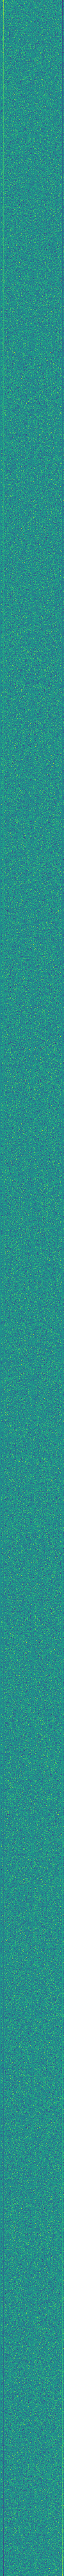
\includegraphics[interpolate=false,width=1.000000in,height=1.000000in]{antiderivative_ci_5-img0.png}}%
\end{pgfscope}%
\begin{pgfscope}%
\pgfsetbuttcap%
\pgfsetroundjoin%
\definecolor{currentfill}{rgb}{0.000000,0.000000,0.000000}%
\pgfsetfillcolor{currentfill}%
\pgfsetlinewidth{0.803000pt}%
\definecolor{currentstroke}{rgb}{0.000000,0.000000,0.000000}%
\pgfsetstrokecolor{currentstroke}%
\pgfsetdash{}{0pt}%
\pgfsys@defobject{currentmarker}{\pgfqpoint{0.000000in}{-0.048611in}}{\pgfqpoint{0.000000in}{0.000000in}}{%
\pgfpathmoveto{\pgfqpoint{0.000000in}{0.000000in}}%
\pgfpathlineto{\pgfqpoint{0.000000in}{-0.048611in}}%
\pgfusepath{stroke,fill}%
}%
\begin{pgfscope}%
\pgfsys@transformshift{0.779897in}{0.517039in}%
\pgfsys@useobject{currentmarker}{}%
\end{pgfscope}%
\end{pgfscope}%
\begin{pgfscope}%
\definecolor{textcolor}{rgb}{0.000000,0.000000,0.000000}%
\pgfsetstrokecolor{textcolor}%
\pgfsetfillcolor{textcolor}%
\pgftext[x=0.779897in,y=0.419816in,,top]{\color{textcolor}{\rmfamily\fontsize{12.000000}{14.400000}\selectfont\catcode`\^=\active\def^{\ifmmode\sp\else\^{}\fi}\catcode`\%=\active\def%{\%}0}}%
\end{pgfscope}%
\begin{pgfscope}%
\pgfsetbuttcap%
\pgfsetroundjoin%
\definecolor{currentfill}{rgb}{0.000000,0.000000,0.000000}%
\pgfsetfillcolor{currentfill}%
\pgfsetlinewidth{0.803000pt}%
\definecolor{currentstroke}{rgb}{0.000000,0.000000,0.000000}%
\pgfsetstrokecolor{currentstroke}%
\pgfsetdash{}{0pt}%
\pgfsys@defobject{currentmarker}{\pgfqpoint{0.000000in}{-0.048611in}}{\pgfqpoint{0.000000in}{0.000000in}}{%
\pgfpathmoveto{\pgfqpoint{0.000000in}{0.000000in}}%
\pgfpathlineto{\pgfqpoint{0.000000in}{-0.048611in}}%
\pgfusepath{stroke,fill}%
}%
\begin{pgfscope}%
\pgfsys@transformshift{1.693017in}{0.517039in}%
\pgfsys@useobject{currentmarker}{}%
\end{pgfscope}%
\end{pgfscope}%
\begin{pgfscope}%
\definecolor{textcolor}{rgb}{0.000000,0.000000,0.000000}%
\pgfsetstrokecolor{textcolor}%
\pgfsetfillcolor{textcolor}%
\pgftext[x=1.693017in,y=0.419816in,,top]{\color{textcolor}{\rmfamily\fontsize{12.000000}{14.400000}\selectfont\catcode`\^=\active\def^{\ifmmode\sp\else\^{}\fi}\catcode`\%=\active\def%{\%}20}}%
\end{pgfscope}%
\begin{pgfscope}%
\pgfsetbuttcap%
\pgfsetroundjoin%
\definecolor{currentfill}{rgb}{0.000000,0.000000,0.000000}%
\pgfsetfillcolor{currentfill}%
\pgfsetlinewidth{0.803000pt}%
\definecolor{currentstroke}{rgb}{0.000000,0.000000,0.000000}%
\pgfsetstrokecolor{currentstroke}%
\pgfsetdash{}{0pt}%
\pgfsys@defobject{currentmarker}{\pgfqpoint{0.000000in}{-0.048611in}}{\pgfqpoint{0.000000in}{0.000000in}}{%
\pgfpathmoveto{\pgfqpoint{0.000000in}{0.000000in}}%
\pgfpathlineto{\pgfqpoint{0.000000in}{-0.048611in}}%
\pgfusepath{stroke,fill}%
}%
\begin{pgfscope}%
\pgfsys@transformshift{2.606137in}{0.517039in}%
\pgfsys@useobject{currentmarker}{}%
\end{pgfscope}%
\end{pgfscope}%
\begin{pgfscope}%
\definecolor{textcolor}{rgb}{0.000000,0.000000,0.000000}%
\pgfsetstrokecolor{textcolor}%
\pgfsetfillcolor{textcolor}%
\pgftext[x=2.606137in,y=0.419816in,,top]{\color{textcolor}{\rmfamily\fontsize{12.000000}{14.400000}\selectfont\catcode`\^=\active\def^{\ifmmode\sp\else\^{}\fi}\catcode`\%=\active\def%{\%}40}}%
\end{pgfscope}%
\begin{pgfscope}%
\definecolor{textcolor}{rgb}{0.000000,0.000000,0.000000}%
\pgfsetstrokecolor{textcolor}%
\pgfsetfillcolor{textcolor}%
\pgftext[x=1.921297in,y=0.202965in,,top]{\color{textcolor}{\rmfamily\fontsize{12.000000}{14.400000}\selectfont\catcode`\^=\active\def^{\ifmmode\sp\else\^{}\fi}\catcode`\%=\active\def%{\%}input coefficients}}%
\end{pgfscope}%
\begin{pgfscope}%
\pgfsetbuttcap%
\pgfsetroundjoin%
\definecolor{currentfill}{rgb}{0.000000,0.000000,0.000000}%
\pgfsetfillcolor{currentfill}%
\pgfsetlinewidth{0.803000pt}%
\definecolor{currentstroke}{rgb}{0.000000,0.000000,0.000000}%
\pgfsetstrokecolor{currentstroke}%
\pgfsetdash{}{0pt}%
\pgfsys@defobject{currentmarker}{\pgfqpoint{-0.048611in}{0.000000in}}{\pgfqpoint{-0.000000in}{0.000000in}}{%
\pgfpathmoveto{\pgfqpoint{-0.000000in}{0.000000in}}%
\pgfpathlineto{\pgfqpoint{-0.048611in}{0.000000in}}%
\pgfusepath{stroke,fill}%
}%
\begin{pgfscope}%
\pgfsys@transformshift{0.779897in}{2.895016in}%
\pgfsys@useobject{currentmarker}{}%
\end{pgfscope}%
\end{pgfscope}%
\begin{pgfscope}%
\definecolor{textcolor}{rgb}{0.000000,0.000000,0.000000}%
\pgfsetstrokecolor{textcolor}%
\pgfsetfillcolor{textcolor}%
\pgftext[x=0.576636in, y=2.831702in, left, base]{\color{textcolor}{\rmfamily\fontsize{12.000000}{14.400000}\selectfont\catcode`\^=\active\def^{\ifmmode\sp\else\^{}\fi}\catcode`\%=\active\def%{\%}0}}%
\end{pgfscope}%
\begin{pgfscope}%
\pgfsetbuttcap%
\pgfsetroundjoin%
\definecolor{currentfill}{rgb}{0.000000,0.000000,0.000000}%
\pgfsetfillcolor{currentfill}%
\pgfsetlinewidth{0.803000pt}%
\definecolor{currentstroke}{rgb}{0.000000,0.000000,0.000000}%
\pgfsetstrokecolor{currentstroke}%
\pgfsetdash{}{0pt}%
\pgfsys@defobject{currentmarker}{\pgfqpoint{-0.048611in}{0.000000in}}{\pgfqpoint{-0.000000in}{0.000000in}}{%
\pgfpathmoveto{\pgfqpoint{-0.000000in}{0.000000in}}%
\pgfpathlineto{\pgfqpoint{-0.048611in}{0.000000in}}%
\pgfusepath{stroke,fill}%
}%
\begin{pgfscope}%
\pgfsys@transformshift{0.779897in}{2.300522in}%
\pgfsys@useobject{currentmarker}{}%
\end{pgfscope}%
\end{pgfscope}%
\begin{pgfscope}%
\definecolor{textcolor}{rgb}{0.000000,0.000000,0.000000}%
\pgfsetstrokecolor{textcolor}%
\pgfsetfillcolor{textcolor}%
\pgftext[x=0.258521in, y=2.237208in, left, base]{\color{textcolor}{\rmfamily\fontsize{12.000000}{14.400000}\selectfont\catcode`\^=\active\def^{\ifmmode\sp\else\^{}\fi}\catcode`\%=\active\def%{\%}1000}}%
\end{pgfscope}%
\begin{pgfscope}%
\pgfsetbuttcap%
\pgfsetroundjoin%
\definecolor{currentfill}{rgb}{0.000000,0.000000,0.000000}%
\pgfsetfillcolor{currentfill}%
\pgfsetlinewidth{0.803000pt}%
\definecolor{currentstroke}{rgb}{0.000000,0.000000,0.000000}%
\pgfsetstrokecolor{currentstroke}%
\pgfsetdash{}{0pt}%
\pgfsys@defobject{currentmarker}{\pgfqpoint{-0.048611in}{0.000000in}}{\pgfqpoint{-0.000000in}{0.000000in}}{%
\pgfpathmoveto{\pgfqpoint{-0.000000in}{0.000000in}}%
\pgfpathlineto{\pgfqpoint{-0.048611in}{0.000000in}}%
\pgfusepath{stroke,fill}%
}%
\begin{pgfscope}%
\pgfsys@transformshift{0.779897in}{1.706027in}%
\pgfsys@useobject{currentmarker}{}%
\end{pgfscope}%
\end{pgfscope}%
\begin{pgfscope}%
\definecolor{textcolor}{rgb}{0.000000,0.000000,0.000000}%
\pgfsetstrokecolor{textcolor}%
\pgfsetfillcolor{textcolor}%
\pgftext[x=0.258521in, y=1.642714in, left, base]{\color{textcolor}{\rmfamily\fontsize{12.000000}{14.400000}\selectfont\catcode`\^=\active\def^{\ifmmode\sp\else\^{}\fi}\catcode`\%=\active\def%{\%}2000}}%
\end{pgfscope}%
\begin{pgfscope}%
\pgfsetbuttcap%
\pgfsetroundjoin%
\definecolor{currentfill}{rgb}{0.000000,0.000000,0.000000}%
\pgfsetfillcolor{currentfill}%
\pgfsetlinewidth{0.803000pt}%
\definecolor{currentstroke}{rgb}{0.000000,0.000000,0.000000}%
\pgfsetstrokecolor{currentstroke}%
\pgfsetdash{}{0pt}%
\pgfsys@defobject{currentmarker}{\pgfqpoint{-0.048611in}{0.000000in}}{\pgfqpoint{-0.000000in}{0.000000in}}{%
\pgfpathmoveto{\pgfqpoint{-0.000000in}{0.000000in}}%
\pgfpathlineto{\pgfqpoint{-0.048611in}{0.000000in}}%
\pgfusepath{stroke,fill}%
}%
\begin{pgfscope}%
\pgfsys@transformshift{0.779897in}{1.111533in}%
\pgfsys@useobject{currentmarker}{}%
\end{pgfscope}%
\end{pgfscope}%
\begin{pgfscope}%
\definecolor{textcolor}{rgb}{0.000000,0.000000,0.000000}%
\pgfsetstrokecolor{textcolor}%
\pgfsetfillcolor{textcolor}%
\pgftext[x=0.258521in, y=1.048219in, left, base]{\color{textcolor}{\rmfamily\fontsize{12.000000}{14.400000}\selectfont\catcode`\^=\active\def^{\ifmmode\sp\else\^{}\fi}\catcode`\%=\active\def%{\%}3000}}%
\end{pgfscope}%
\begin{pgfscope}%
\pgfsetbuttcap%
\pgfsetroundjoin%
\definecolor{currentfill}{rgb}{0.000000,0.000000,0.000000}%
\pgfsetfillcolor{currentfill}%
\pgfsetlinewidth{0.803000pt}%
\definecolor{currentstroke}{rgb}{0.000000,0.000000,0.000000}%
\pgfsetstrokecolor{currentstroke}%
\pgfsetdash{}{0pt}%
\pgfsys@defobject{currentmarker}{\pgfqpoint{-0.048611in}{0.000000in}}{\pgfqpoint{-0.000000in}{0.000000in}}{%
\pgfpathmoveto{\pgfqpoint{-0.000000in}{0.000000in}}%
\pgfpathlineto{\pgfqpoint{-0.048611in}{0.000000in}}%
\pgfusepath{stroke,fill}%
}%
\begin{pgfscope}%
\pgfsys@transformshift{0.779897in}{0.517039in}%
\pgfsys@useobject{currentmarker}{}%
\end{pgfscope}%
\end{pgfscope}%
\begin{pgfscope}%
\definecolor{textcolor}{rgb}{0.000000,0.000000,0.000000}%
\pgfsetstrokecolor{textcolor}%
\pgfsetfillcolor{textcolor}%
\pgftext[x=0.258521in, y=0.453725in, left, base]{\color{textcolor}{\rmfamily\fontsize{12.000000}{14.400000}\selectfont\catcode`\^=\active\def^{\ifmmode\sp\else\^{}\fi}\catcode`\%=\active\def%{\%}4000}}%
\end{pgfscope}%
\begin{pgfscope}%
\definecolor{textcolor}{rgb}{0.000000,0.000000,0.000000}%
\pgfsetstrokecolor{textcolor}%
\pgfsetfillcolor{textcolor}%
\pgftext[x=0.202965in,y=1.706027in,,bottom,rotate=90.000000]{\color{textcolor}{\rmfamily\fontsize{12.000000}{14.400000}\selectfont\catcode`\^=\active\def^{\ifmmode\sp\else\^{}\fi}\catcode`\%=\active\def%{\%}samples}}%
\end{pgfscope}%
\begin{pgfscope}%
\pgfsetrectcap%
\pgfsetmiterjoin%
\pgfsetlinewidth{0.803000pt}%
\definecolor{currentstroke}{rgb}{0.000000,0.000000,0.000000}%
\pgfsetstrokecolor{currentstroke}%
\pgfsetdash{}{0pt}%
\pgfpathmoveto{\pgfqpoint{0.779897in}{0.517039in}}%
\pgfpathlineto{\pgfqpoint{0.779897in}{2.895016in}}%
\pgfusepath{stroke}%
\end{pgfscope}%
\begin{pgfscope}%
\pgfsetrectcap%
\pgfsetmiterjoin%
\pgfsetlinewidth{0.803000pt}%
\definecolor{currentstroke}{rgb}{0.000000,0.000000,0.000000}%
\pgfsetstrokecolor{currentstroke}%
\pgfsetdash{}{0pt}%
\pgfpathmoveto{\pgfqpoint{3.062697in}{0.517039in}}%
\pgfpathlineto{\pgfqpoint{3.062697in}{2.895016in}}%
\pgfusepath{stroke}%
\end{pgfscope}%
\begin{pgfscope}%
\pgfsetrectcap%
\pgfsetmiterjoin%
\pgfsetlinewidth{0.803000pt}%
\definecolor{currentstroke}{rgb}{0.000000,0.000000,0.000000}%
\pgfsetstrokecolor{currentstroke}%
\pgfsetdash{}{0pt}%
\pgfpathmoveto{\pgfqpoint{0.779897in}{0.517039in}}%
\pgfpathlineto{\pgfqpoint{3.062697in}{0.517039in}}%
\pgfusepath{stroke}%
\end{pgfscope}%
\begin{pgfscope}%
\pgfsetrectcap%
\pgfsetmiterjoin%
\pgfsetlinewidth{0.803000pt}%
\definecolor{currentstroke}{rgb}{0.000000,0.000000,0.000000}%
\pgfsetstrokecolor{currentstroke}%
\pgfsetdash{}{0pt}%
\pgfpathmoveto{\pgfqpoint{0.779897in}{2.895016in}}%
\pgfpathlineto{\pgfqpoint{3.062697in}{2.895016in}}%
\pgfusepath{stroke}%
\end{pgfscope}%
\begin{pgfscope}%
\pgfsetbuttcap%
\pgfsetmiterjoin%
\pgfsetlinewidth{0.000000pt}%
\definecolor{currentstroke}{rgb}{0.000000,0.000000,0.000000}%
\pgfsetstrokecolor{currentstroke}%
\pgfsetstrokeopacity{0.000000}%
\pgfsetdash{}{0pt}%
\pgfpathmoveto{\pgfqpoint{3.282875in}{0.517039in}}%
\pgfpathlineto{\pgfqpoint{3.401774in}{0.517039in}}%
\pgfpathlineto{\pgfqpoint{3.401774in}{2.895016in}}%
\pgfpathlineto{\pgfqpoint{3.282875in}{2.895016in}}%
\pgfpathlineto{\pgfqpoint{3.282875in}{0.517039in}}%
\pgfpathclose%
\pgfusepath{}%
\end{pgfscope}%
\begin{pgfscope}%
\pgfsys@transformshift{3.280000in}{0.520000in}%
\pgftext[left,bottom]{
\includegraphics[interpolate=true,width=0.120000in,height=2.380000in]{antiderivative_ci_5-img1.png}}%
\end{pgfscope}%
\begin{pgfscope}%
\pgfsetbuttcap%
\pgfsetroundjoin%
\definecolor{currentfill}{rgb}{0.000000,0.000000,0.000000}%
\pgfsetfillcolor{currentfill}%
\pgfsetlinewidth{0.803000pt}%
\definecolor{currentstroke}{rgb}{0.000000,0.000000,0.000000}%
\pgfsetstrokecolor{currentstroke}%
\pgfsetdash{}{0pt}%
\pgfsys@defobject{currentmarker}{\pgfqpoint{0.000000in}{0.000000in}}{\pgfqpoint{0.048611in}{0.000000in}}{%
\pgfpathmoveto{\pgfqpoint{0.000000in}{0.000000in}}%
\pgfpathlineto{\pgfqpoint{0.048611in}{0.000000in}}%
\pgfusepath{stroke,fill}%
}%
\begin{pgfscope}%
\pgfsys@transformshift{3.401774in}{0.636505in}%
\pgfsys@useobject{currentmarker}{}%
\end{pgfscope}%
\end{pgfscope}%
\begin{pgfscope}%
\definecolor{textcolor}{rgb}{0.000000,0.000000,0.000000}%
\pgfsetstrokecolor{textcolor}%
\pgfsetfillcolor{textcolor}%
\pgftext[x=3.498996in, y=0.573191in, left, base]{\color{textcolor}{\rmfamily\fontsize{12.000000}{14.400000}\selectfont\catcode`\^=\active\def^{\ifmmode\sp\else\^{}\fi}\catcode`\%=\active\def%{\%}\ensuremath{-}100}}%
\end{pgfscope}%
\begin{pgfscope}%
\pgfsetbuttcap%
\pgfsetroundjoin%
\definecolor{currentfill}{rgb}{0.000000,0.000000,0.000000}%
\pgfsetfillcolor{currentfill}%
\pgfsetlinewidth{0.803000pt}%
\definecolor{currentstroke}{rgb}{0.000000,0.000000,0.000000}%
\pgfsetstrokecolor{currentstroke}%
\pgfsetdash{}{0pt}%
\pgfsys@defobject{currentmarker}{\pgfqpoint{0.000000in}{0.000000in}}{\pgfqpoint{0.048611in}{0.000000in}}{%
\pgfpathmoveto{\pgfqpoint{0.000000in}{0.000000in}}%
\pgfpathlineto{\pgfqpoint{0.048611in}{0.000000in}}%
\pgfusepath{stroke,fill}%
}%
\begin{pgfscope}%
\pgfsys@transformshift{3.401774in}{1.171266in}%
\pgfsys@useobject{currentmarker}{}%
\end{pgfscope}%
\end{pgfscope}%
\begin{pgfscope}%
\definecolor{textcolor}{rgb}{0.000000,0.000000,0.000000}%
\pgfsetstrokecolor{textcolor}%
\pgfsetfillcolor{textcolor}%
\pgftext[x=3.498996in, y=1.107952in, left, base]{\color{textcolor}{\rmfamily\fontsize{12.000000}{14.400000}\selectfont\catcode`\^=\active\def^{\ifmmode\sp\else\^{}\fi}\catcode`\%=\active\def%{\%}\ensuremath{-}50}}%
\end{pgfscope}%
\begin{pgfscope}%
\pgfsetbuttcap%
\pgfsetroundjoin%
\definecolor{currentfill}{rgb}{0.000000,0.000000,0.000000}%
\pgfsetfillcolor{currentfill}%
\pgfsetlinewidth{0.803000pt}%
\definecolor{currentstroke}{rgb}{0.000000,0.000000,0.000000}%
\pgfsetstrokecolor{currentstroke}%
\pgfsetdash{}{0pt}%
\pgfsys@defobject{currentmarker}{\pgfqpoint{0.000000in}{0.000000in}}{\pgfqpoint{0.048611in}{0.000000in}}{%
\pgfpathmoveto{\pgfqpoint{0.000000in}{0.000000in}}%
\pgfpathlineto{\pgfqpoint{0.048611in}{0.000000in}}%
\pgfusepath{stroke,fill}%
}%
\begin{pgfscope}%
\pgfsys@transformshift{3.401774in}{1.706028in}%
\pgfsys@useobject{currentmarker}{}%
\end{pgfscope}%
\end{pgfscope}%
\begin{pgfscope}%
\definecolor{textcolor}{rgb}{0.000000,0.000000,0.000000}%
\pgfsetstrokecolor{textcolor}%
\pgfsetfillcolor{textcolor}%
\pgftext[x=3.498996in, y=1.642714in, left, base]{\color{textcolor}{\rmfamily\fontsize{12.000000}{14.400000}\selectfont\catcode`\^=\active\def^{\ifmmode\sp\else\^{}\fi}\catcode`\%=\active\def%{\%}0}}%
\end{pgfscope}%
\begin{pgfscope}%
\pgfsetbuttcap%
\pgfsetroundjoin%
\definecolor{currentfill}{rgb}{0.000000,0.000000,0.000000}%
\pgfsetfillcolor{currentfill}%
\pgfsetlinewidth{0.803000pt}%
\definecolor{currentstroke}{rgb}{0.000000,0.000000,0.000000}%
\pgfsetstrokecolor{currentstroke}%
\pgfsetdash{}{0pt}%
\pgfsys@defobject{currentmarker}{\pgfqpoint{0.000000in}{0.000000in}}{\pgfqpoint{0.048611in}{0.000000in}}{%
\pgfpathmoveto{\pgfqpoint{0.000000in}{0.000000in}}%
\pgfpathlineto{\pgfqpoint{0.048611in}{0.000000in}}%
\pgfusepath{stroke,fill}%
}%
\begin{pgfscope}%
\pgfsys@transformshift{3.401774in}{2.240789in}%
\pgfsys@useobject{currentmarker}{}%
\end{pgfscope}%
\end{pgfscope}%
\begin{pgfscope}%
\definecolor{textcolor}{rgb}{0.000000,0.000000,0.000000}%
\pgfsetstrokecolor{textcolor}%
\pgfsetfillcolor{textcolor}%
\pgftext[x=3.498996in, y=2.177475in, left, base]{\color{textcolor}{\rmfamily\fontsize{12.000000}{14.400000}\selectfont\catcode`\^=\active\def^{\ifmmode\sp\else\^{}\fi}\catcode`\%=\active\def%{\%}50}}%
\end{pgfscope}%
\begin{pgfscope}%
\pgfsetbuttcap%
\pgfsetroundjoin%
\definecolor{currentfill}{rgb}{0.000000,0.000000,0.000000}%
\pgfsetfillcolor{currentfill}%
\pgfsetlinewidth{0.803000pt}%
\definecolor{currentstroke}{rgb}{0.000000,0.000000,0.000000}%
\pgfsetstrokecolor{currentstroke}%
\pgfsetdash{}{0pt}%
\pgfsys@defobject{currentmarker}{\pgfqpoint{0.000000in}{0.000000in}}{\pgfqpoint{0.048611in}{0.000000in}}{%
\pgfpathmoveto{\pgfqpoint{0.000000in}{0.000000in}}%
\pgfpathlineto{\pgfqpoint{0.048611in}{0.000000in}}%
\pgfusepath{stroke,fill}%
}%
\begin{pgfscope}%
\pgfsys@transformshift{3.401774in}{2.775550in}%
\pgfsys@useobject{currentmarker}{}%
\end{pgfscope}%
\end{pgfscope}%
\begin{pgfscope}%
\definecolor{textcolor}{rgb}{0.000000,0.000000,0.000000}%
\pgfsetstrokecolor{textcolor}%
\pgfsetfillcolor{textcolor}%
\pgftext[x=3.498996in, y=2.712237in, left, base]{\color{textcolor}{\rmfamily\fontsize{12.000000}{14.400000}\selectfont\catcode`\^=\active\def^{\ifmmode\sp\else\^{}\fi}\catcode`\%=\active\def%{\%}100}}%
\end{pgfscope}%
\begin{pgfscope}%
\pgfsetrectcap%
\pgfsetmiterjoin%
\pgfsetlinewidth{0.803000pt}%
\definecolor{currentstroke}{rgb}{0.000000,0.000000,0.000000}%
\pgfsetstrokecolor{currentstroke}%
\pgfsetdash{}{0pt}%
\pgfpathmoveto{\pgfqpoint{3.282875in}{0.517039in}}%
\pgfpathlineto{\pgfqpoint{3.342325in}{0.517039in}}%
\pgfpathlineto{\pgfqpoint{3.401774in}{0.517039in}}%
\pgfpathlineto{\pgfqpoint{3.401774in}{2.895016in}}%
\pgfpathlineto{\pgfqpoint{3.342325in}{2.895016in}}%
\pgfpathlineto{\pgfqpoint{3.282875in}{2.895016in}}%
\pgfpathlineto{\pgfqpoint{3.282875in}{0.517039in}}%
\pgfpathclose%
\pgfusepath{stroke}%
\end{pgfscope}%
\end{pgfpicture}%
\makeatother%
\endgroup%

      \end{adjustbox}
      \caption{Correlation image 5\% noise.}\label{fig:sc1_ci_5}
    \end{subfigure}
    \begin{subfigure}{0.49\linewidth}
      \begin{adjustbox}{width=\linewidth}
        \begingroup%
\makeatletter%
\begin{pgfpicture}%
\pgfpathrectangle{\pgfpointorigin}{\pgfqpoint{6.400000in}{4.800000in}}%
\pgfusepath{use as bounding box, clip}%
\begin{pgfscope}%
\pgfsetbuttcap%
\pgfsetmiterjoin%
\pgfsetlinewidth{0.000000pt}%
\definecolor{currentstroke}{rgb}{0.000000,0.000000,0.000000}%
\pgfsetstrokecolor{currentstroke}%
\pgfsetstrokeopacity{0.000000}%
\pgfsetdash{}{0pt}%
\pgfpathmoveto{\pgfqpoint{0.000000in}{0.000000in}}%
\pgfpathlineto{\pgfqpoint{6.400000in}{0.000000in}}%
\pgfpathlineto{\pgfqpoint{6.400000in}{4.800000in}}%
\pgfpathlineto{\pgfqpoint{0.000000in}{4.800000in}}%
\pgfpathlineto{\pgfqpoint{0.000000in}{0.000000in}}%
\pgfpathclose%
\pgfusepath{}%
\end{pgfscope}%
\begin{pgfscope}%
\pgfsetbuttcap%
\pgfsetmiterjoin%
\pgfsetlinewidth{0.000000pt}%
\definecolor{currentstroke}{rgb}{0.000000,0.000000,0.000000}%
\pgfsetstrokecolor{currentstroke}%
\pgfsetstrokeopacity{0.000000}%
\pgfsetdash{}{0pt}%
\pgfpathmoveto{\pgfqpoint{1.072000in}{0.528000in}}%
\pgfpathlineto{\pgfqpoint{4.768000in}{0.528000in}}%
\pgfpathlineto{\pgfqpoint{4.768000in}{4.224000in}}%
\pgfpathlineto{\pgfqpoint{1.072000in}{4.224000in}}%
\pgfpathlineto{\pgfqpoint{1.072000in}{0.528000in}}%
\pgfpathclose%
\pgfusepath{}%
\end{pgfscope}%
\begin{pgfscope}%
\pgfpathrectangle{\pgfqpoint{1.072000in}{0.528000in}}{\pgfqpoint{3.696000in}{3.696000in}}%
\pgfusepath{clip}%
\pgfsys@transformcm{3.696000}{0.000000}{0.000000}{-3.696000}{1.072000in}{4.224000in}%
\pgftext[left,bottom]{
\includegraphics[interpolate=false,width=1.000000in,height=1.000000in]{antiderivative_pm_5-img0.png}}%
\end{pgfscope}%
\begin{pgfscope}%
\pgfsetbuttcap%
\pgfsetroundjoin%
\definecolor{currentfill}{rgb}{0.000000,0.000000,0.000000}%
\pgfsetfillcolor{currentfill}%
\pgfsetlinewidth{0.803000pt}%
\definecolor{currentstroke}{rgb}{0.000000,0.000000,0.000000}%
\pgfsetstrokecolor{currentstroke}%
\pgfsetdash{}{0pt}%
\pgfsys@defobject{currentmarker}{\pgfqpoint{0.000000in}{-0.048611in}}{\pgfqpoint{0.000000in}{0.000000in}}{%
\pgfpathmoveto{\pgfqpoint{0.000000in}{0.000000in}}%
\pgfpathlineto{\pgfqpoint{0.000000in}{-0.048611in}}%
\pgfusepath{stroke,fill}%
}%
\begin{pgfscope}%
\pgfsys@transformshift{1.090480in}{0.528000in}%
\pgfsys@useobject{currentmarker}{}%
\end{pgfscope}%
\end{pgfscope}%
\begin{pgfscope}%
\definecolor{textcolor}{rgb}{0.000000,0.000000,0.000000}%
\pgfsetstrokecolor{textcolor}%
\pgfsetfillcolor{textcolor}%
\pgftext[x=1.090480in,y=0.430778in,,top]{\color{textcolor}{\rmfamily\fontsize{12.000000}{14.400000}\selectfont\catcode`\^=\active\def^{\ifmmode\sp\else\^{}\fi}\catcode`\%=\active\def%{\%}0}}%
\end{pgfscope}%
\begin{pgfscope}%
\pgfsetbuttcap%
\pgfsetroundjoin%
\definecolor{currentfill}{rgb}{0.000000,0.000000,0.000000}%
\pgfsetfillcolor{currentfill}%
\pgfsetlinewidth{0.803000pt}%
\definecolor{currentstroke}{rgb}{0.000000,0.000000,0.000000}%
\pgfsetstrokecolor{currentstroke}%
\pgfsetdash{}{0pt}%
\pgfsys@defobject{currentmarker}{\pgfqpoint{0.000000in}{-0.048611in}}{\pgfqpoint{0.000000in}{0.000000in}}{%
\pgfpathmoveto{\pgfqpoint{0.000000in}{0.000000in}}%
\pgfpathlineto{\pgfqpoint{0.000000in}{-0.048611in}}%
\pgfusepath{stroke,fill}%
}%
\begin{pgfscope}%
\pgfsys@transformshift{1.829680in}{0.528000in}%
\pgfsys@useobject{currentmarker}{}%
\end{pgfscope}%
\end{pgfscope}%
\begin{pgfscope}%
\definecolor{textcolor}{rgb}{0.000000,0.000000,0.000000}%
\pgfsetstrokecolor{textcolor}%
\pgfsetfillcolor{textcolor}%
\pgftext[x=1.829680in,y=0.430778in,,top]{\color{textcolor}{\rmfamily\fontsize{12.000000}{14.400000}\selectfont\catcode`\^=\active\def^{\ifmmode\sp\else\^{}\fi}\catcode`\%=\active\def%{\%}20}}%
\end{pgfscope}%
\begin{pgfscope}%
\pgfsetbuttcap%
\pgfsetroundjoin%
\definecolor{currentfill}{rgb}{0.000000,0.000000,0.000000}%
\pgfsetfillcolor{currentfill}%
\pgfsetlinewidth{0.803000pt}%
\definecolor{currentstroke}{rgb}{0.000000,0.000000,0.000000}%
\pgfsetstrokecolor{currentstroke}%
\pgfsetdash{}{0pt}%
\pgfsys@defobject{currentmarker}{\pgfqpoint{0.000000in}{-0.048611in}}{\pgfqpoint{0.000000in}{0.000000in}}{%
\pgfpathmoveto{\pgfqpoint{0.000000in}{0.000000in}}%
\pgfpathlineto{\pgfqpoint{0.000000in}{-0.048611in}}%
\pgfusepath{stroke,fill}%
}%
\begin{pgfscope}%
\pgfsys@transformshift{2.568880in}{0.528000in}%
\pgfsys@useobject{currentmarker}{}%
\end{pgfscope}%
\end{pgfscope}%
\begin{pgfscope}%
\definecolor{textcolor}{rgb}{0.000000,0.000000,0.000000}%
\pgfsetstrokecolor{textcolor}%
\pgfsetfillcolor{textcolor}%
\pgftext[x=2.568880in,y=0.430778in,,top]{\color{textcolor}{\rmfamily\fontsize{12.000000}{14.400000}\selectfont\catcode`\^=\active\def^{\ifmmode\sp\else\^{}\fi}\catcode`\%=\active\def%{\%}40}}%
\end{pgfscope}%
\begin{pgfscope}%
\pgfsetbuttcap%
\pgfsetroundjoin%
\definecolor{currentfill}{rgb}{0.000000,0.000000,0.000000}%
\pgfsetfillcolor{currentfill}%
\pgfsetlinewidth{0.803000pt}%
\definecolor{currentstroke}{rgb}{0.000000,0.000000,0.000000}%
\pgfsetstrokecolor{currentstroke}%
\pgfsetdash{}{0pt}%
\pgfsys@defobject{currentmarker}{\pgfqpoint{0.000000in}{-0.048611in}}{\pgfqpoint{0.000000in}{0.000000in}}{%
\pgfpathmoveto{\pgfqpoint{0.000000in}{0.000000in}}%
\pgfpathlineto{\pgfqpoint{0.000000in}{-0.048611in}}%
\pgfusepath{stroke,fill}%
}%
\begin{pgfscope}%
\pgfsys@transformshift{3.308080in}{0.528000in}%
\pgfsys@useobject{currentmarker}{}%
\end{pgfscope}%
\end{pgfscope}%
\begin{pgfscope}%
\definecolor{textcolor}{rgb}{0.000000,0.000000,0.000000}%
\pgfsetstrokecolor{textcolor}%
\pgfsetfillcolor{textcolor}%
\pgftext[x=3.308080in,y=0.430778in,,top]{\color{textcolor}{\rmfamily\fontsize{12.000000}{14.400000}\selectfont\catcode`\^=\active\def^{\ifmmode\sp\else\^{}\fi}\catcode`\%=\active\def%{\%}60}}%
\end{pgfscope}%
\begin{pgfscope}%
\pgfsetbuttcap%
\pgfsetroundjoin%
\definecolor{currentfill}{rgb}{0.000000,0.000000,0.000000}%
\pgfsetfillcolor{currentfill}%
\pgfsetlinewidth{0.803000pt}%
\definecolor{currentstroke}{rgb}{0.000000,0.000000,0.000000}%
\pgfsetstrokecolor{currentstroke}%
\pgfsetdash{}{0pt}%
\pgfsys@defobject{currentmarker}{\pgfqpoint{0.000000in}{-0.048611in}}{\pgfqpoint{0.000000in}{0.000000in}}{%
\pgfpathmoveto{\pgfqpoint{0.000000in}{0.000000in}}%
\pgfpathlineto{\pgfqpoint{0.000000in}{-0.048611in}}%
\pgfusepath{stroke,fill}%
}%
\begin{pgfscope}%
\pgfsys@transformshift{4.047280in}{0.528000in}%
\pgfsys@useobject{currentmarker}{}%
\end{pgfscope}%
\end{pgfscope}%
\begin{pgfscope}%
\definecolor{textcolor}{rgb}{0.000000,0.000000,0.000000}%
\pgfsetstrokecolor{textcolor}%
\pgfsetfillcolor{textcolor}%
\pgftext[x=4.047280in,y=0.430778in,,top]{\color{textcolor}{\rmfamily\fontsize{12.000000}{14.400000}\selectfont\catcode`\^=\active\def^{\ifmmode\sp\else\^{}\fi}\catcode`\%=\active\def%{\%}80}}%
\end{pgfscope}%
\begin{pgfscope}%
\definecolor{textcolor}{rgb}{0.000000,0.000000,0.000000}%
\pgfsetstrokecolor{textcolor}%
\pgfsetfillcolor{textcolor}%
\pgftext[x=2.920000in,y=0.213927in,,top]{\color{textcolor}{\rmfamily\fontsize{12.000000}{14.400000}\selectfont\catcode`\^=\active\def^{\ifmmode\sp\else\^{}\fi}\catcode`\%=\active\def%{\%}output coefficients}}%
\end{pgfscope}%
\begin{pgfscope}%
\pgfsetbuttcap%
\pgfsetroundjoin%
\definecolor{currentfill}{rgb}{0.000000,0.000000,0.000000}%
\pgfsetfillcolor{currentfill}%
\pgfsetlinewidth{0.803000pt}%
\definecolor{currentstroke}{rgb}{0.000000,0.000000,0.000000}%
\pgfsetstrokecolor{currentstroke}%
\pgfsetdash{}{0pt}%
\pgfsys@defobject{currentmarker}{\pgfqpoint{-0.048611in}{0.000000in}}{\pgfqpoint{-0.000000in}{0.000000in}}{%
\pgfpathmoveto{\pgfqpoint{-0.000000in}{0.000000in}}%
\pgfpathlineto{\pgfqpoint{-0.048611in}{0.000000in}}%
\pgfusepath{stroke,fill}%
}%
\begin{pgfscope}%
\pgfsys@transformshift{1.072000in}{4.205520in}%
\pgfsys@useobject{currentmarker}{}%
\end{pgfscope}%
\end{pgfscope}%
\begin{pgfscope}%
\definecolor{textcolor}{rgb}{0.000000,0.000000,0.000000}%
\pgfsetstrokecolor{textcolor}%
\pgfsetfillcolor{textcolor}%
\pgftext[x=0.868739in, y=4.142206in, left, base]{\color{textcolor}{\rmfamily\fontsize{12.000000}{14.400000}\selectfont\catcode`\^=\active\def^{\ifmmode\sp\else\^{}\fi}\catcode`\%=\active\def%{\%}0}}%
\end{pgfscope}%
\begin{pgfscope}%
\pgfsetbuttcap%
\pgfsetroundjoin%
\definecolor{currentfill}{rgb}{0.000000,0.000000,0.000000}%
\pgfsetfillcolor{currentfill}%
\pgfsetlinewidth{0.803000pt}%
\definecolor{currentstroke}{rgb}{0.000000,0.000000,0.000000}%
\pgfsetstrokecolor{currentstroke}%
\pgfsetdash{}{0pt}%
\pgfsys@defobject{currentmarker}{\pgfqpoint{-0.048611in}{0.000000in}}{\pgfqpoint{-0.000000in}{0.000000in}}{%
\pgfpathmoveto{\pgfqpoint{-0.000000in}{0.000000in}}%
\pgfpathlineto{\pgfqpoint{-0.048611in}{0.000000in}}%
\pgfusepath{stroke,fill}%
}%
\begin{pgfscope}%
\pgfsys@transformshift{1.072000in}{3.466320in}%
\pgfsys@useobject{currentmarker}{}%
\end{pgfscope}%
\end{pgfscope}%
\begin{pgfscope}%
\definecolor{textcolor}{rgb}{0.000000,0.000000,0.000000}%
\pgfsetstrokecolor{textcolor}%
\pgfsetfillcolor{textcolor}%
\pgftext[x=0.762701in, y=3.403006in, left, base]{\color{textcolor}{\rmfamily\fontsize{12.000000}{14.400000}\selectfont\catcode`\^=\active\def^{\ifmmode\sp\else\^{}\fi}\catcode`\%=\active\def%{\%}20}}%
\end{pgfscope}%
\begin{pgfscope}%
\pgfsetbuttcap%
\pgfsetroundjoin%
\definecolor{currentfill}{rgb}{0.000000,0.000000,0.000000}%
\pgfsetfillcolor{currentfill}%
\pgfsetlinewidth{0.803000pt}%
\definecolor{currentstroke}{rgb}{0.000000,0.000000,0.000000}%
\pgfsetstrokecolor{currentstroke}%
\pgfsetdash{}{0pt}%
\pgfsys@defobject{currentmarker}{\pgfqpoint{-0.048611in}{0.000000in}}{\pgfqpoint{-0.000000in}{0.000000in}}{%
\pgfpathmoveto{\pgfqpoint{-0.000000in}{0.000000in}}%
\pgfpathlineto{\pgfqpoint{-0.048611in}{0.000000in}}%
\pgfusepath{stroke,fill}%
}%
\begin{pgfscope}%
\pgfsys@transformshift{1.072000in}{2.727120in}%
\pgfsys@useobject{currentmarker}{}%
\end{pgfscope}%
\end{pgfscope}%
\begin{pgfscope}%
\definecolor{textcolor}{rgb}{0.000000,0.000000,0.000000}%
\pgfsetstrokecolor{textcolor}%
\pgfsetfillcolor{textcolor}%
\pgftext[x=0.762701in, y=2.663806in, left, base]{\color{textcolor}{\rmfamily\fontsize{12.000000}{14.400000}\selectfont\catcode`\^=\active\def^{\ifmmode\sp\else\^{}\fi}\catcode`\%=\active\def%{\%}40}}%
\end{pgfscope}%
\begin{pgfscope}%
\pgfsetbuttcap%
\pgfsetroundjoin%
\definecolor{currentfill}{rgb}{0.000000,0.000000,0.000000}%
\pgfsetfillcolor{currentfill}%
\pgfsetlinewidth{0.803000pt}%
\definecolor{currentstroke}{rgb}{0.000000,0.000000,0.000000}%
\pgfsetstrokecolor{currentstroke}%
\pgfsetdash{}{0pt}%
\pgfsys@defobject{currentmarker}{\pgfqpoint{-0.048611in}{0.000000in}}{\pgfqpoint{-0.000000in}{0.000000in}}{%
\pgfpathmoveto{\pgfqpoint{-0.000000in}{0.000000in}}%
\pgfpathlineto{\pgfqpoint{-0.048611in}{0.000000in}}%
\pgfusepath{stroke,fill}%
}%
\begin{pgfscope}%
\pgfsys@transformshift{1.072000in}{1.987920in}%
\pgfsys@useobject{currentmarker}{}%
\end{pgfscope}%
\end{pgfscope}%
\begin{pgfscope}%
\definecolor{textcolor}{rgb}{0.000000,0.000000,0.000000}%
\pgfsetstrokecolor{textcolor}%
\pgfsetfillcolor{textcolor}%
\pgftext[x=0.762701in, y=1.924606in, left, base]{\color{textcolor}{\rmfamily\fontsize{12.000000}{14.400000}\selectfont\catcode`\^=\active\def^{\ifmmode\sp\else\^{}\fi}\catcode`\%=\active\def%{\%}60}}%
\end{pgfscope}%
\begin{pgfscope}%
\pgfsetbuttcap%
\pgfsetroundjoin%
\definecolor{currentfill}{rgb}{0.000000,0.000000,0.000000}%
\pgfsetfillcolor{currentfill}%
\pgfsetlinewidth{0.803000pt}%
\definecolor{currentstroke}{rgb}{0.000000,0.000000,0.000000}%
\pgfsetstrokecolor{currentstroke}%
\pgfsetdash{}{0pt}%
\pgfsys@defobject{currentmarker}{\pgfqpoint{-0.048611in}{0.000000in}}{\pgfqpoint{-0.000000in}{0.000000in}}{%
\pgfpathmoveto{\pgfqpoint{-0.000000in}{0.000000in}}%
\pgfpathlineto{\pgfqpoint{-0.048611in}{0.000000in}}%
\pgfusepath{stroke,fill}%
}%
\begin{pgfscope}%
\pgfsys@transformshift{1.072000in}{1.248720in}%
\pgfsys@useobject{currentmarker}{}%
\end{pgfscope}%
\end{pgfscope}%
\begin{pgfscope}%
\definecolor{textcolor}{rgb}{0.000000,0.000000,0.000000}%
\pgfsetstrokecolor{textcolor}%
\pgfsetfillcolor{textcolor}%
\pgftext[x=0.762701in, y=1.185406in, left, base]{\color{textcolor}{\rmfamily\fontsize{12.000000}{14.400000}\selectfont\catcode`\^=\active\def^{\ifmmode\sp\else\^{}\fi}\catcode`\%=\active\def%{\%}80}}%
\end{pgfscope}%
\begin{pgfscope}%
\definecolor{textcolor}{rgb}{0.000000,0.000000,0.000000}%
\pgfsetstrokecolor{textcolor}%
\pgfsetfillcolor{textcolor}%
\pgftext[x=0.707145in,y=2.376000in,,bottom,rotate=90.000000]{\color{textcolor}{\rmfamily\fontsize{12.000000}{14.400000}\selectfont\catcode`\^=\active\def^{\ifmmode\sp\else\^{}\fi}\catcode`\%=\active\def%{\%}input coefficients}}%
\end{pgfscope}%
\begin{pgfscope}%
\pgfsetrectcap%
\pgfsetmiterjoin%
\pgfsetlinewidth{0.803000pt}%
\definecolor{currentstroke}{rgb}{0.000000,0.000000,0.000000}%
\pgfsetstrokecolor{currentstroke}%
\pgfsetdash{}{0pt}%
\pgfpathmoveto{\pgfqpoint{1.072000in}{0.528000in}}%
\pgfpathlineto{\pgfqpoint{1.072000in}{4.224000in}}%
\pgfusepath{stroke}%
\end{pgfscope}%
\begin{pgfscope}%
\pgfsetrectcap%
\pgfsetmiterjoin%
\pgfsetlinewidth{0.803000pt}%
\definecolor{currentstroke}{rgb}{0.000000,0.000000,0.000000}%
\pgfsetstrokecolor{currentstroke}%
\pgfsetdash{}{0pt}%
\pgfpathmoveto{\pgfqpoint{4.768000in}{0.528000in}}%
\pgfpathlineto{\pgfqpoint{4.768000in}{4.224000in}}%
\pgfusepath{stroke}%
\end{pgfscope}%
\begin{pgfscope}%
\pgfsetrectcap%
\pgfsetmiterjoin%
\pgfsetlinewidth{0.803000pt}%
\definecolor{currentstroke}{rgb}{0.000000,0.000000,0.000000}%
\pgfsetstrokecolor{currentstroke}%
\pgfsetdash{}{0pt}%
\pgfpathmoveto{\pgfqpoint{1.072000in}{0.528000in}}%
\pgfpathlineto{\pgfqpoint{4.768000in}{0.528000in}}%
\pgfusepath{stroke}%
\end{pgfscope}%
\begin{pgfscope}%
\pgfsetrectcap%
\pgfsetmiterjoin%
\pgfsetlinewidth{0.803000pt}%
\definecolor{currentstroke}{rgb}{0.000000,0.000000,0.000000}%
\pgfsetstrokecolor{currentstroke}%
\pgfsetdash{}{0pt}%
\pgfpathmoveto{\pgfqpoint{1.072000in}{4.224000in}}%
\pgfpathlineto{\pgfqpoint{4.768000in}{4.224000in}}%
\pgfusepath{stroke}%
\end{pgfscope}%
\begin{pgfscope}%
\pgfsetbuttcap%
\pgfsetmiterjoin%
\pgfsetlinewidth{0.000000pt}%
\definecolor{currentstroke}{rgb}{0.000000,0.000000,0.000000}%
\pgfsetstrokecolor{currentstroke}%
\pgfsetstrokeopacity{0.000000}%
\pgfsetdash{}{0pt}%
\pgfpathmoveto{\pgfqpoint{5.016000in}{0.528000in}}%
\pgfpathlineto{\pgfqpoint{5.200800in}{0.528000in}}%
\pgfpathlineto{\pgfqpoint{5.200800in}{4.224000in}}%
\pgfpathlineto{\pgfqpoint{5.016000in}{4.224000in}}%
\pgfpathlineto{\pgfqpoint{5.016000in}{0.528000in}}%
\pgfpathclose%
\pgfusepath{}%
\end{pgfscope}%
\begin{pgfscope}%
\pgfsys@transformshift{5.020000in}{0.530000in}%
\pgftext[left,bottom]{
\includegraphics[interpolate=true,width=0.180000in,height=3.690000in]{antiderivative_pm_5-img1.png}}%
\end{pgfscope}%
\begin{pgfscope}%
\pgfsetbuttcap%
\pgfsetroundjoin%
\definecolor{currentfill}{rgb}{0.000000,0.000000,0.000000}%
\pgfsetfillcolor{currentfill}%
\pgfsetlinewidth{0.803000pt}%
\definecolor{currentstroke}{rgb}{0.000000,0.000000,0.000000}%
\pgfsetstrokecolor{currentstroke}%
\pgfsetdash{}{0pt}%
\pgfsys@defobject{currentmarker}{\pgfqpoint{0.000000in}{0.000000in}}{\pgfqpoint{0.048611in}{0.000000in}}{%
\pgfpathmoveto{\pgfqpoint{0.000000in}{0.000000in}}%
\pgfpathlineto{\pgfqpoint{0.048611in}{0.000000in}}%
\pgfusepath{stroke,fill}%
}%
\begin{pgfscope}%
\pgfsys@transformshift{5.200800in}{0.806760in}%
\pgfsys@useobject{currentmarker}{}%
\end{pgfscope}%
\end{pgfscope}%
\begin{pgfscope}%
\definecolor{textcolor}{rgb}{0.000000,0.000000,0.000000}%
\pgfsetstrokecolor{textcolor}%
\pgfsetfillcolor{textcolor}%
\pgftext[x=5.298022in, y=0.743447in, left, base]{\color{textcolor}{\rmfamily\fontsize{12.000000}{14.400000}\selectfont\catcode`\^=\active\def^{\ifmmode\sp\else\^{}\fi}\catcode`\%=\active\def%{\%}\ensuremath{-}2000}}%
\end{pgfscope}%
\begin{pgfscope}%
\pgfsetbuttcap%
\pgfsetroundjoin%
\definecolor{currentfill}{rgb}{0.000000,0.000000,0.000000}%
\pgfsetfillcolor{currentfill}%
\pgfsetlinewidth{0.803000pt}%
\definecolor{currentstroke}{rgb}{0.000000,0.000000,0.000000}%
\pgfsetstrokecolor{currentstroke}%
\pgfsetdash{}{0pt}%
\pgfsys@defobject{currentmarker}{\pgfqpoint{0.000000in}{0.000000in}}{\pgfqpoint{0.048611in}{0.000000in}}{%
\pgfpathmoveto{\pgfqpoint{0.000000in}{0.000000in}}%
\pgfpathlineto{\pgfqpoint{0.048611in}{0.000000in}}%
\pgfusepath{stroke,fill}%
}%
\begin{pgfscope}%
\pgfsys@transformshift{5.200800in}{1.404820in}%
\pgfsys@useobject{currentmarker}{}%
\end{pgfscope}%
\end{pgfscope}%
\begin{pgfscope}%
\definecolor{textcolor}{rgb}{0.000000,0.000000,0.000000}%
\pgfsetstrokecolor{textcolor}%
\pgfsetfillcolor{textcolor}%
\pgftext[x=5.298022in, y=1.341506in, left, base]{\color{textcolor}{\rmfamily\fontsize{12.000000}{14.400000}\selectfont\catcode`\^=\active\def^{\ifmmode\sp\else\^{}\fi}\catcode`\%=\active\def%{\%}\ensuremath{-}1500}}%
\end{pgfscope}%
\begin{pgfscope}%
\pgfsetbuttcap%
\pgfsetroundjoin%
\definecolor{currentfill}{rgb}{0.000000,0.000000,0.000000}%
\pgfsetfillcolor{currentfill}%
\pgfsetlinewidth{0.803000pt}%
\definecolor{currentstroke}{rgb}{0.000000,0.000000,0.000000}%
\pgfsetstrokecolor{currentstroke}%
\pgfsetdash{}{0pt}%
\pgfsys@defobject{currentmarker}{\pgfqpoint{0.000000in}{0.000000in}}{\pgfqpoint{0.048611in}{0.000000in}}{%
\pgfpathmoveto{\pgfqpoint{0.000000in}{0.000000in}}%
\pgfpathlineto{\pgfqpoint{0.048611in}{0.000000in}}%
\pgfusepath{stroke,fill}%
}%
\begin{pgfscope}%
\pgfsys@transformshift{5.200800in}{2.002880in}%
\pgfsys@useobject{currentmarker}{}%
\end{pgfscope}%
\end{pgfscope}%
\begin{pgfscope}%
\definecolor{textcolor}{rgb}{0.000000,0.000000,0.000000}%
\pgfsetstrokecolor{textcolor}%
\pgfsetfillcolor{textcolor}%
\pgftext[x=5.298022in, y=1.939566in, left, base]{\color{textcolor}{\rmfamily\fontsize{12.000000}{14.400000}\selectfont\catcode`\^=\active\def^{\ifmmode\sp\else\^{}\fi}\catcode`\%=\active\def%{\%}\ensuremath{-}1000}}%
\end{pgfscope}%
\begin{pgfscope}%
\pgfsetbuttcap%
\pgfsetroundjoin%
\definecolor{currentfill}{rgb}{0.000000,0.000000,0.000000}%
\pgfsetfillcolor{currentfill}%
\pgfsetlinewidth{0.803000pt}%
\definecolor{currentstroke}{rgb}{0.000000,0.000000,0.000000}%
\pgfsetstrokecolor{currentstroke}%
\pgfsetdash{}{0pt}%
\pgfsys@defobject{currentmarker}{\pgfqpoint{0.000000in}{0.000000in}}{\pgfqpoint{0.048611in}{0.000000in}}{%
\pgfpathmoveto{\pgfqpoint{0.000000in}{0.000000in}}%
\pgfpathlineto{\pgfqpoint{0.048611in}{0.000000in}}%
\pgfusepath{stroke,fill}%
}%
\begin{pgfscope}%
\pgfsys@transformshift{5.200800in}{2.600940in}%
\pgfsys@useobject{currentmarker}{}%
\end{pgfscope}%
\end{pgfscope}%
\begin{pgfscope}%
\definecolor{textcolor}{rgb}{0.000000,0.000000,0.000000}%
\pgfsetstrokecolor{textcolor}%
\pgfsetfillcolor{textcolor}%
\pgftext[x=5.298022in, y=2.537626in, left, base]{\color{textcolor}{\rmfamily\fontsize{12.000000}{14.400000}\selectfont\catcode`\^=\active\def^{\ifmmode\sp\else\^{}\fi}\catcode`\%=\active\def%{\%}\ensuremath{-}500}}%
\end{pgfscope}%
\begin{pgfscope}%
\pgfsetbuttcap%
\pgfsetroundjoin%
\definecolor{currentfill}{rgb}{0.000000,0.000000,0.000000}%
\pgfsetfillcolor{currentfill}%
\pgfsetlinewidth{0.803000pt}%
\definecolor{currentstroke}{rgb}{0.000000,0.000000,0.000000}%
\pgfsetstrokecolor{currentstroke}%
\pgfsetdash{}{0pt}%
\pgfsys@defobject{currentmarker}{\pgfqpoint{0.000000in}{0.000000in}}{\pgfqpoint{0.048611in}{0.000000in}}{%
\pgfpathmoveto{\pgfqpoint{0.000000in}{0.000000in}}%
\pgfpathlineto{\pgfqpoint{0.048611in}{0.000000in}}%
\pgfusepath{stroke,fill}%
}%
\begin{pgfscope}%
\pgfsys@transformshift{5.200800in}{3.199000in}%
\pgfsys@useobject{currentmarker}{}%
\end{pgfscope}%
\end{pgfscope}%
\begin{pgfscope}%
\definecolor{textcolor}{rgb}{0.000000,0.000000,0.000000}%
\pgfsetstrokecolor{textcolor}%
\pgfsetfillcolor{textcolor}%
\pgftext[x=5.298022in, y=3.135686in, left, base]{\color{textcolor}{\rmfamily\fontsize{12.000000}{14.400000}\selectfont\catcode`\^=\active\def^{\ifmmode\sp\else\^{}\fi}\catcode`\%=\active\def%{\%}0}}%
\end{pgfscope}%
\begin{pgfscope}%
\pgfsetbuttcap%
\pgfsetroundjoin%
\definecolor{currentfill}{rgb}{0.000000,0.000000,0.000000}%
\pgfsetfillcolor{currentfill}%
\pgfsetlinewidth{0.803000pt}%
\definecolor{currentstroke}{rgb}{0.000000,0.000000,0.000000}%
\pgfsetstrokecolor{currentstroke}%
\pgfsetdash{}{0pt}%
\pgfsys@defobject{currentmarker}{\pgfqpoint{0.000000in}{0.000000in}}{\pgfqpoint{0.048611in}{0.000000in}}{%
\pgfpathmoveto{\pgfqpoint{0.000000in}{0.000000in}}%
\pgfpathlineto{\pgfqpoint{0.048611in}{0.000000in}}%
\pgfusepath{stroke,fill}%
}%
\begin{pgfscope}%
\pgfsys@transformshift{5.200800in}{3.797059in}%
\pgfsys@useobject{currentmarker}{}%
\end{pgfscope}%
\end{pgfscope}%
\begin{pgfscope}%
\definecolor{textcolor}{rgb}{0.000000,0.000000,0.000000}%
\pgfsetstrokecolor{textcolor}%
\pgfsetfillcolor{textcolor}%
\pgftext[x=5.298022in, y=3.733746in, left, base]{\color{textcolor}{\rmfamily\fontsize{12.000000}{14.400000}\selectfont\catcode`\^=\active\def^{\ifmmode\sp\else\^{}\fi}\catcode`\%=\active\def%{\%}500}}%
\end{pgfscope}%
\begin{pgfscope}%
\pgfsetrectcap%
\pgfsetmiterjoin%
\pgfsetlinewidth{0.803000pt}%
\definecolor{currentstroke}{rgb}{0.000000,0.000000,0.000000}%
\pgfsetstrokecolor{currentstroke}%
\pgfsetdash{}{0pt}%
\pgfpathmoveto{\pgfqpoint{5.016000in}{0.528000in}}%
\pgfpathlineto{\pgfqpoint{5.108400in}{0.528000in}}%
\pgfpathlineto{\pgfqpoint{5.200800in}{0.528000in}}%
\pgfpathlineto{\pgfqpoint{5.200800in}{4.224000in}}%
\pgfpathlineto{\pgfqpoint{5.108400in}{4.224000in}}%
\pgfpathlineto{\pgfqpoint{5.016000in}{4.224000in}}%
\pgfpathlineto{\pgfqpoint{5.016000in}{0.528000in}}%
\pgfpathclose%
\pgfusepath{stroke}%
\end{pgfscope}%
\end{pgfpicture}%
\makeatother%
\endgroup%

      \end{adjustbox}
      \caption{The p-matrix for 5\% noise.}\label{fig:sc1_pm_5}
    \end{subfigure}
    % \\[\baselineskip]
    \begin{subfigure}{0.49\linewidth}
      \begin{adjustbox}{width=\linewidth}
        \begingroup%
\makeatletter%
\begin{pgfpicture}%
\pgfpathrectangle{\pgfpointorigin}{\pgfqpoint{6.400000in}{4.800000in}}%
\pgfusepath{use as bounding box, clip}%
\begin{pgfscope}%
\pgfsetbuttcap%
\pgfsetmiterjoin%
\pgfsetlinewidth{0.000000pt}%
\definecolor{currentstroke}{rgb}{0.000000,0.000000,0.000000}%
\pgfsetstrokecolor{currentstroke}%
\pgfsetstrokeopacity{0.000000}%
\pgfsetdash{}{0pt}%
\pgfpathmoveto{\pgfqpoint{0.000000in}{0.000000in}}%
\pgfpathlineto{\pgfqpoint{6.400000in}{0.000000in}}%
\pgfpathlineto{\pgfqpoint{6.400000in}{4.800000in}}%
\pgfpathlineto{\pgfqpoint{0.000000in}{4.800000in}}%
\pgfpathlineto{\pgfqpoint{0.000000in}{0.000000in}}%
\pgfpathclose%
\pgfusepath{}%
\end{pgfscope}%
\begin{pgfscope}%
\pgfsetbuttcap%
\pgfsetmiterjoin%
\pgfsetlinewidth{0.000000pt}%
\definecolor{currentstroke}{rgb}{0.000000,0.000000,0.000000}%
\pgfsetstrokecolor{currentstroke}%
\pgfsetstrokeopacity{0.000000}%
\pgfsetdash{}{0pt}%
\pgfpathmoveto{\pgfqpoint{0.800000in}{0.528000in}}%
\pgfpathlineto{\pgfqpoint{4.768000in}{0.528000in}}%
\pgfpathlineto{\pgfqpoint{4.768000in}{4.224000in}}%
\pgfpathlineto{\pgfqpoint{0.800000in}{4.224000in}}%
\pgfpathlineto{\pgfqpoint{0.800000in}{0.528000in}}%
\pgfpathclose%
\pgfusepath{}%
\end{pgfscope}%
\begin{pgfscope}%
\pgfpathrectangle{\pgfqpoint{0.800000in}{0.528000in}}{\pgfqpoint{3.968000in}{3.696000in}}%
\pgfusepath{clip}%
\pgfsys@transformcm{3.968000}{0.000000}{0.000000}{-3.696000}{0.800000in}{4.224000in}%
\pgftext[left,bottom]{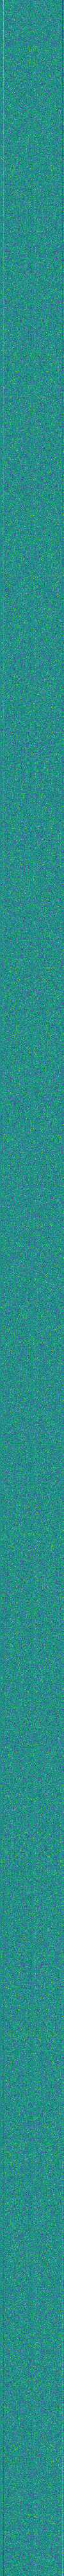
\includegraphics[interpolate=false,width=1.000000in,height=1.000000in]{antiderivative_ci_10-img0.png}}%
\end{pgfscope}%
\begin{pgfscope}%
\pgfsetbuttcap%
\pgfsetroundjoin%
\definecolor{currentfill}{rgb}{0.000000,0.000000,0.000000}%
\pgfsetfillcolor{currentfill}%
\pgfsetlinewidth{0.803000pt}%
\definecolor{currentstroke}{rgb}{0.000000,0.000000,0.000000}%
\pgfsetstrokecolor{currentstroke}%
\pgfsetdash{}{0pt}%
\pgfsys@defobject{currentmarker}{\pgfqpoint{0.000000in}{-0.048611in}}{\pgfqpoint{0.000000in}{0.000000in}}{%
\pgfpathmoveto{\pgfqpoint{0.000000in}{0.000000in}}%
\pgfpathlineto{\pgfqpoint{0.000000in}{-0.048611in}}%
\pgfusepath{stroke,fill}%
}%
\begin{pgfscope}%
\pgfsys@transformshift{0.800000in}{0.528000in}%
\pgfsys@useobject{currentmarker}{}%
\end{pgfscope}%
\end{pgfscope}%
\begin{pgfscope}%
\definecolor{textcolor}{rgb}{0.000000,0.000000,0.000000}%
\pgfsetstrokecolor{textcolor}%
\pgfsetfillcolor{textcolor}%
\pgftext[x=0.800000in,y=0.430778in,,top]{\color{textcolor}{\rmfamily\fontsize{12.000000}{14.400000}\selectfont\catcode`\^=\active\def^{\ifmmode\sp\else\^{}\fi}\catcode`\%=\active\def%{\%}0}}%
\end{pgfscope}%
\begin{pgfscope}%
\pgfsetbuttcap%
\pgfsetroundjoin%
\definecolor{currentfill}{rgb}{0.000000,0.000000,0.000000}%
\pgfsetfillcolor{currentfill}%
\pgfsetlinewidth{0.803000pt}%
\definecolor{currentstroke}{rgb}{0.000000,0.000000,0.000000}%
\pgfsetstrokecolor{currentstroke}%
\pgfsetdash{}{0pt}%
\pgfsys@defobject{currentmarker}{\pgfqpoint{0.000000in}{-0.048611in}}{\pgfqpoint{0.000000in}{0.000000in}}{%
\pgfpathmoveto{\pgfqpoint{0.000000in}{0.000000in}}%
\pgfpathlineto{\pgfqpoint{0.000000in}{-0.048611in}}%
\pgfusepath{stroke,fill}%
}%
\begin{pgfscope}%
\pgfsys@transformshift{1.593600in}{0.528000in}%
\pgfsys@useobject{currentmarker}{}%
\end{pgfscope}%
\end{pgfscope}%
\begin{pgfscope}%
\definecolor{textcolor}{rgb}{0.000000,0.000000,0.000000}%
\pgfsetstrokecolor{textcolor}%
\pgfsetfillcolor{textcolor}%
\pgftext[x=1.593600in,y=0.430778in,,top]{\color{textcolor}{\rmfamily\fontsize{12.000000}{14.400000}\selectfont\catcode`\^=\active\def^{\ifmmode\sp\else\^{}\fi}\catcode`\%=\active\def%{\%}10}}%
\end{pgfscope}%
\begin{pgfscope}%
\pgfsetbuttcap%
\pgfsetroundjoin%
\definecolor{currentfill}{rgb}{0.000000,0.000000,0.000000}%
\pgfsetfillcolor{currentfill}%
\pgfsetlinewidth{0.803000pt}%
\definecolor{currentstroke}{rgb}{0.000000,0.000000,0.000000}%
\pgfsetstrokecolor{currentstroke}%
\pgfsetdash{}{0pt}%
\pgfsys@defobject{currentmarker}{\pgfqpoint{0.000000in}{-0.048611in}}{\pgfqpoint{0.000000in}{0.000000in}}{%
\pgfpathmoveto{\pgfqpoint{0.000000in}{0.000000in}}%
\pgfpathlineto{\pgfqpoint{0.000000in}{-0.048611in}}%
\pgfusepath{stroke,fill}%
}%
\begin{pgfscope}%
\pgfsys@transformshift{2.387200in}{0.528000in}%
\pgfsys@useobject{currentmarker}{}%
\end{pgfscope}%
\end{pgfscope}%
\begin{pgfscope}%
\definecolor{textcolor}{rgb}{0.000000,0.000000,0.000000}%
\pgfsetstrokecolor{textcolor}%
\pgfsetfillcolor{textcolor}%
\pgftext[x=2.387200in,y=0.430778in,,top]{\color{textcolor}{\rmfamily\fontsize{12.000000}{14.400000}\selectfont\catcode`\^=\active\def^{\ifmmode\sp\else\^{}\fi}\catcode`\%=\active\def%{\%}20}}%
\end{pgfscope}%
\begin{pgfscope}%
\pgfsetbuttcap%
\pgfsetroundjoin%
\definecolor{currentfill}{rgb}{0.000000,0.000000,0.000000}%
\pgfsetfillcolor{currentfill}%
\pgfsetlinewidth{0.803000pt}%
\definecolor{currentstroke}{rgb}{0.000000,0.000000,0.000000}%
\pgfsetstrokecolor{currentstroke}%
\pgfsetdash{}{0pt}%
\pgfsys@defobject{currentmarker}{\pgfqpoint{0.000000in}{-0.048611in}}{\pgfqpoint{0.000000in}{0.000000in}}{%
\pgfpathmoveto{\pgfqpoint{0.000000in}{0.000000in}}%
\pgfpathlineto{\pgfqpoint{0.000000in}{-0.048611in}}%
\pgfusepath{stroke,fill}%
}%
\begin{pgfscope}%
\pgfsys@transformshift{3.180800in}{0.528000in}%
\pgfsys@useobject{currentmarker}{}%
\end{pgfscope}%
\end{pgfscope}%
\begin{pgfscope}%
\definecolor{textcolor}{rgb}{0.000000,0.000000,0.000000}%
\pgfsetstrokecolor{textcolor}%
\pgfsetfillcolor{textcolor}%
\pgftext[x=3.180800in,y=0.430778in,,top]{\color{textcolor}{\rmfamily\fontsize{12.000000}{14.400000}\selectfont\catcode`\^=\active\def^{\ifmmode\sp\else\^{}\fi}\catcode`\%=\active\def%{\%}30}}%
\end{pgfscope}%
\begin{pgfscope}%
\pgfsetbuttcap%
\pgfsetroundjoin%
\definecolor{currentfill}{rgb}{0.000000,0.000000,0.000000}%
\pgfsetfillcolor{currentfill}%
\pgfsetlinewidth{0.803000pt}%
\definecolor{currentstroke}{rgb}{0.000000,0.000000,0.000000}%
\pgfsetstrokecolor{currentstroke}%
\pgfsetdash{}{0pt}%
\pgfsys@defobject{currentmarker}{\pgfqpoint{0.000000in}{-0.048611in}}{\pgfqpoint{0.000000in}{0.000000in}}{%
\pgfpathmoveto{\pgfqpoint{0.000000in}{0.000000in}}%
\pgfpathlineto{\pgfqpoint{0.000000in}{-0.048611in}}%
\pgfusepath{stroke,fill}%
}%
\begin{pgfscope}%
\pgfsys@transformshift{3.974400in}{0.528000in}%
\pgfsys@useobject{currentmarker}{}%
\end{pgfscope}%
\end{pgfscope}%
\begin{pgfscope}%
\definecolor{textcolor}{rgb}{0.000000,0.000000,0.000000}%
\pgfsetstrokecolor{textcolor}%
\pgfsetfillcolor{textcolor}%
\pgftext[x=3.974400in,y=0.430778in,,top]{\color{textcolor}{\rmfamily\fontsize{12.000000}{14.400000}\selectfont\catcode`\^=\active\def^{\ifmmode\sp\else\^{}\fi}\catcode`\%=\active\def%{\%}40}}%
\end{pgfscope}%
\begin{pgfscope}%
\pgfsetbuttcap%
\pgfsetroundjoin%
\definecolor{currentfill}{rgb}{0.000000,0.000000,0.000000}%
\pgfsetfillcolor{currentfill}%
\pgfsetlinewidth{0.803000pt}%
\definecolor{currentstroke}{rgb}{0.000000,0.000000,0.000000}%
\pgfsetstrokecolor{currentstroke}%
\pgfsetdash{}{0pt}%
\pgfsys@defobject{currentmarker}{\pgfqpoint{0.000000in}{-0.048611in}}{\pgfqpoint{0.000000in}{0.000000in}}{%
\pgfpathmoveto{\pgfqpoint{0.000000in}{0.000000in}}%
\pgfpathlineto{\pgfqpoint{0.000000in}{-0.048611in}}%
\pgfusepath{stroke,fill}%
}%
\begin{pgfscope}%
\pgfsys@transformshift{4.768000in}{0.528000in}%
\pgfsys@useobject{currentmarker}{}%
\end{pgfscope}%
\end{pgfscope}%
\begin{pgfscope}%
\definecolor{textcolor}{rgb}{0.000000,0.000000,0.000000}%
\pgfsetstrokecolor{textcolor}%
\pgfsetfillcolor{textcolor}%
\pgftext[x=4.768000in,y=0.430778in,,top]{\color{textcolor}{\rmfamily\fontsize{12.000000}{14.400000}\selectfont\catcode`\^=\active\def^{\ifmmode\sp\else\^{}\fi}\catcode`\%=\active\def%{\%}50}}%
\end{pgfscope}%
\begin{pgfscope}%
\definecolor{textcolor}{rgb}{0.000000,0.000000,0.000000}%
\pgfsetstrokecolor{textcolor}%
\pgfsetfillcolor{textcolor}%
\pgftext[x=2.784000in,y=0.213927in,,top]{\color{textcolor}{\rmfamily\fontsize{12.000000}{14.400000}\selectfont\catcode`\^=\active\def^{\ifmmode\sp\else\^{}\fi}\catcode`\%=\active\def%{\%}input coefficients}}%
\end{pgfscope}%
\begin{pgfscope}%
\pgfsetbuttcap%
\pgfsetroundjoin%
\definecolor{currentfill}{rgb}{0.000000,0.000000,0.000000}%
\pgfsetfillcolor{currentfill}%
\pgfsetlinewidth{0.803000pt}%
\definecolor{currentstroke}{rgb}{0.000000,0.000000,0.000000}%
\pgfsetstrokecolor{currentstroke}%
\pgfsetdash{}{0pt}%
\pgfsys@defobject{currentmarker}{\pgfqpoint{-0.048611in}{0.000000in}}{\pgfqpoint{-0.000000in}{0.000000in}}{%
\pgfpathmoveto{\pgfqpoint{-0.000000in}{0.000000in}}%
\pgfpathlineto{\pgfqpoint{-0.048611in}{0.000000in}}%
\pgfusepath{stroke,fill}%
}%
\begin{pgfscope}%
\pgfsys@transformshift{0.800000in}{4.224000in}%
\pgfsys@useobject{currentmarker}{}%
\end{pgfscope}%
\end{pgfscope}%
\begin{pgfscope}%
\definecolor{textcolor}{rgb}{0.000000,0.000000,0.000000}%
\pgfsetstrokecolor{textcolor}%
\pgfsetfillcolor{textcolor}%
\pgftext[x=0.596739in, y=4.160686in, left, base]{\color{textcolor}{\rmfamily\fontsize{12.000000}{14.400000}\selectfont\catcode`\^=\active\def^{\ifmmode\sp\else\^{}\fi}\catcode`\%=\active\def%{\%}0}}%
\end{pgfscope}%
\begin{pgfscope}%
\pgfsetbuttcap%
\pgfsetroundjoin%
\definecolor{currentfill}{rgb}{0.000000,0.000000,0.000000}%
\pgfsetfillcolor{currentfill}%
\pgfsetlinewidth{0.803000pt}%
\definecolor{currentstroke}{rgb}{0.000000,0.000000,0.000000}%
\pgfsetstrokecolor{currentstroke}%
\pgfsetdash{}{0pt}%
\pgfsys@defobject{currentmarker}{\pgfqpoint{-0.048611in}{0.000000in}}{\pgfqpoint{-0.000000in}{0.000000in}}{%
\pgfpathmoveto{\pgfqpoint{-0.000000in}{0.000000in}}%
\pgfpathlineto{\pgfqpoint{-0.048611in}{0.000000in}}%
\pgfusepath{stroke,fill}%
}%
\begin{pgfscope}%
\pgfsys@transformshift{0.800000in}{3.762000in}%
\pgfsys@useobject{currentmarker}{}%
\end{pgfscope}%
\end{pgfscope}%
\begin{pgfscope}%
\definecolor{textcolor}{rgb}{0.000000,0.000000,0.000000}%
\pgfsetstrokecolor{textcolor}%
\pgfsetfillcolor{textcolor}%
\pgftext[x=0.384662in, y=3.698686in, left, base]{\color{textcolor}{\rmfamily\fontsize{12.000000}{14.400000}\selectfont\catcode`\^=\active\def^{\ifmmode\sp\else\^{}\fi}\catcode`\%=\active\def%{\%}500}}%
\end{pgfscope}%
\begin{pgfscope}%
\pgfsetbuttcap%
\pgfsetroundjoin%
\definecolor{currentfill}{rgb}{0.000000,0.000000,0.000000}%
\pgfsetfillcolor{currentfill}%
\pgfsetlinewidth{0.803000pt}%
\definecolor{currentstroke}{rgb}{0.000000,0.000000,0.000000}%
\pgfsetstrokecolor{currentstroke}%
\pgfsetdash{}{0pt}%
\pgfsys@defobject{currentmarker}{\pgfqpoint{-0.048611in}{0.000000in}}{\pgfqpoint{-0.000000in}{0.000000in}}{%
\pgfpathmoveto{\pgfqpoint{-0.000000in}{0.000000in}}%
\pgfpathlineto{\pgfqpoint{-0.048611in}{0.000000in}}%
\pgfusepath{stroke,fill}%
}%
\begin{pgfscope}%
\pgfsys@transformshift{0.800000in}{3.300000in}%
\pgfsys@useobject{currentmarker}{}%
\end{pgfscope}%
\end{pgfscope}%
\begin{pgfscope}%
\definecolor{textcolor}{rgb}{0.000000,0.000000,0.000000}%
\pgfsetstrokecolor{textcolor}%
\pgfsetfillcolor{textcolor}%
\pgftext[x=0.278624in, y=3.236686in, left, base]{\color{textcolor}{\rmfamily\fontsize{12.000000}{14.400000}\selectfont\catcode`\^=\active\def^{\ifmmode\sp\else\^{}\fi}\catcode`\%=\active\def%{\%}1000}}%
\end{pgfscope}%
\begin{pgfscope}%
\pgfsetbuttcap%
\pgfsetroundjoin%
\definecolor{currentfill}{rgb}{0.000000,0.000000,0.000000}%
\pgfsetfillcolor{currentfill}%
\pgfsetlinewidth{0.803000pt}%
\definecolor{currentstroke}{rgb}{0.000000,0.000000,0.000000}%
\pgfsetstrokecolor{currentstroke}%
\pgfsetdash{}{0pt}%
\pgfsys@defobject{currentmarker}{\pgfqpoint{-0.048611in}{0.000000in}}{\pgfqpoint{-0.000000in}{0.000000in}}{%
\pgfpathmoveto{\pgfqpoint{-0.000000in}{0.000000in}}%
\pgfpathlineto{\pgfqpoint{-0.048611in}{0.000000in}}%
\pgfusepath{stroke,fill}%
}%
\begin{pgfscope}%
\pgfsys@transformshift{0.800000in}{2.838000in}%
\pgfsys@useobject{currentmarker}{}%
\end{pgfscope}%
\end{pgfscope}%
\begin{pgfscope}%
\definecolor{textcolor}{rgb}{0.000000,0.000000,0.000000}%
\pgfsetstrokecolor{textcolor}%
\pgfsetfillcolor{textcolor}%
\pgftext[x=0.278624in, y=2.774686in, left, base]{\color{textcolor}{\rmfamily\fontsize{12.000000}{14.400000}\selectfont\catcode`\^=\active\def^{\ifmmode\sp\else\^{}\fi}\catcode`\%=\active\def%{\%}1500}}%
\end{pgfscope}%
\begin{pgfscope}%
\pgfsetbuttcap%
\pgfsetroundjoin%
\definecolor{currentfill}{rgb}{0.000000,0.000000,0.000000}%
\pgfsetfillcolor{currentfill}%
\pgfsetlinewidth{0.803000pt}%
\definecolor{currentstroke}{rgb}{0.000000,0.000000,0.000000}%
\pgfsetstrokecolor{currentstroke}%
\pgfsetdash{}{0pt}%
\pgfsys@defobject{currentmarker}{\pgfqpoint{-0.048611in}{0.000000in}}{\pgfqpoint{-0.000000in}{0.000000in}}{%
\pgfpathmoveto{\pgfqpoint{-0.000000in}{0.000000in}}%
\pgfpathlineto{\pgfqpoint{-0.048611in}{0.000000in}}%
\pgfusepath{stroke,fill}%
}%
\begin{pgfscope}%
\pgfsys@transformshift{0.800000in}{2.376000in}%
\pgfsys@useobject{currentmarker}{}%
\end{pgfscope}%
\end{pgfscope}%
\begin{pgfscope}%
\definecolor{textcolor}{rgb}{0.000000,0.000000,0.000000}%
\pgfsetstrokecolor{textcolor}%
\pgfsetfillcolor{textcolor}%
\pgftext[x=0.278624in, y=2.312686in, left, base]{\color{textcolor}{\rmfamily\fontsize{12.000000}{14.400000}\selectfont\catcode`\^=\active\def^{\ifmmode\sp\else\^{}\fi}\catcode`\%=\active\def%{\%}2000}}%
\end{pgfscope}%
\begin{pgfscope}%
\pgfsetbuttcap%
\pgfsetroundjoin%
\definecolor{currentfill}{rgb}{0.000000,0.000000,0.000000}%
\pgfsetfillcolor{currentfill}%
\pgfsetlinewidth{0.803000pt}%
\definecolor{currentstroke}{rgb}{0.000000,0.000000,0.000000}%
\pgfsetstrokecolor{currentstroke}%
\pgfsetdash{}{0pt}%
\pgfsys@defobject{currentmarker}{\pgfqpoint{-0.048611in}{0.000000in}}{\pgfqpoint{-0.000000in}{0.000000in}}{%
\pgfpathmoveto{\pgfqpoint{-0.000000in}{0.000000in}}%
\pgfpathlineto{\pgfqpoint{-0.048611in}{0.000000in}}%
\pgfusepath{stroke,fill}%
}%
\begin{pgfscope}%
\pgfsys@transformshift{0.800000in}{1.914000in}%
\pgfsys@useobject{currentmarker}{}%
\end{pgfscope}%
\end{pgfscope}%
\begin{pgfscope}%
\definecolor{textcolor}{rgb}{0.000000,0.000000,0.000000}%
\pgfsetstrokecolor{textcolor}%
\pgfsetfillcolor{textcolor}%
\pgftext[x=0.278624in, y=1.850686in, left, base]{\color{textcolor}{\rmfamily\fontsize{12.000000}{14.400000}\selectfont\catcode`\^=\active\def^{\ifmmode\sp\else\^{}\fi}\catcode`\%=\active\def%{\%}2500}}%
\end{pgfscope}%
\begin{pgfscope}%
\pgfsetbuttcap%
\pgfsetroundjoin%
\definecolor{currentfill}{rgb}{0.000000,0.000000,0.000000}%
\pgfsetfillcolor{currentfill}%
\pgfsetlinewidth{0.803000pt}%
\definecolor{currentstroke}{rgb}{0.000000,0.000000,0.000000}%
\pgfsetstrokecolor{currentstroke}%
\pgfsetdash{}{0pt}%
\pgfsys@defobject{currentmarker}{\pgfqpoint{-0.048611in}{0.000000in}}{\pgfqpoint{-0.000000in}{0.000000in}}{%
\pgfpathmoveto{\pgfqpoint{-0.000000in}{0.000000in}}%
\pgfpathlineto{\pgfqpoint{-0.048611in}{0.000000in}}%
\pgfusepath{stroke,fill}%
}%
\begin{pgfscope}%
\pgfsys@transformshift{0.800000in}{1.452000in}%
\pgfsys@useobject{currentmarker}{}%
\end{pgfscope}%
\end{pgfscope}%
\begin{pgfscope}%
\definecolor{textcolor}{rgb}{0.000000,0.000000,0.000000}%
\pgfsetstrokecolor{textcolor}%
\pgfsetfillcolor{textcolor}%
\pgftext[x=0.278624in, y=1.388686in, left, base]{\color{textcolor}{\rmfamily\fontsize{12.000000}{14.400000}\selectfont\catcode`\^=\active\def^{\ifmmode\sp\else\^{}\fi}\catcode`\%=\active\def%{\%}3000}}%
\end{pgfscope}%
\begin{pgfscope}%
\pgfsetbuttcap%
\pgfsetroundjoin%
\definecolor{currentfill}{rgb}{0.000000,0.000000,0.000000}%
\pgfsetfillcolor{currentfill}%
\pgfsetlinewidth{0.803000pt}%
\definecolor{currentstroke}{rgb}{0.000000,0.000000,0.000000}%
\pgfsetstrokecolor{currentstroke}%
\pgfsetdash{}{0pt}%
\pgfsys@defobject{currentmarker}{\pgfqpoint{-0.048611in}{0.000000in}}{\pgfqpoint{-0.000000in}{0.000000in}}{%
\pgfpathmoveto{\pgfqpoint{-0.000000in}{0.000000in}}%
\pgfpathlineto{\pgfqpoint{-0.048611in}{0.000000in}}%
\pgfusepath{stroke,fill}%
}%
\begin{pgfscope}%
\pgfsys@transformshift{0.800000in}{0.990000in}%
\pgfsys@useobject{currentmarker}{}%
\end{pgfscope}%
\end{pgfscope}%
\begin{pgfscope}%
\definecolor{textcolor}{rgb}{0.000000,0.000000,0.000000}%
\pgfsetstrokecolor{textcolor}%
\pgfsetfillcolor{textcolor}%
\pgftext[x=0.278624in, y=0.926686in, left, base]{\color{textcolor}{\rmfamily\fontsize{12.000000}{14.400000}\selectfont\catcode`\^=\active\def^{\ifmmode\sp\else\^{}\fi}\catcode`\%=\active\def%{\%}3500}}%
\end{pgfscope}%
\begin{pgfscope}%
\pgfsetbuttcap%
\pgfsetroundjoin%
\definecolor{currentfill}{rgb}{0.000000,0.000000,0.000000}%
\pgfsetfillcolor{currentfill}%
\pgfsetlinewidth{0.803000pt}%
\definecolor{currentstroke}{rgb}{0.000000,0.000000,0.000000}%
\pgfsetstrokecolor{currentstroke}%
\pgfsetdash{}{0pt}%
\pgfsys@defobject{currentmarker}{\pgfqpoint{-0.048611in}{0.000000in}}{\pgfqpoint{-0.000000in}{0.000000in}}{%
\pgfpathmoveto{\pgfqpoint{-0.000000in}{0.000000in}}%
\pgfpathlineto{\pgfqpoint{-0.048611in}{0.000000in}}%
\pgfusepath{stroke,fill}%
}%
\begin{pgfscope}%
\pgfsys@transformshift{0.800000in}{0.528000in}%
\pgfsys@useobject{currentmarker}{}%
\end{pgfscope}%
\end{pgfscope}%
\begin{pgfscope}%
\definecolor{textcolor}{rgb}{0.000000,0.000000,0.000000}%
\pgfsetstrokecolor{textcolor}%
\pgfsetfillcolor{textcolor}%
\pgftext[x=0.278624in, y=0.464686in, left, base]{\color{textcolor}{\rmfamily\fontsize{12.000000}{14.400000}\selectfont\catcode`\^=\active\def^{\ifmmode\sp\else\^{}\fi}\catcode`\%=\active\def%{\%}4000}}%
\end{pgfscope}%
\begin{pgfscope}%
\definecolor{textcolor}{rgb}{0.000000,0.000000,0.000000}%
\pgfsetstrokecolor{textcolor}%
\pgfsetfillcolor{textcolor}%
\pgftext[x=0.223069in,y=2.376000in,,bottom,rotate=90.000000]{\color{textcolor}{\rmfamily\fontsize{12.000000}{14.400000}\selectfont\catcode`\^=\active\def^{\ifmmode\sp\else\^{}\fi}\catcode`\%=\active\def%{\%}samples}}%
\end{pgfscope}%
\begin{pgfscope}%
\pgfsetrectcap%
\pgfsetmiterjoin%
\pgfsetlinewidth{0.803000pt}%
\definecolor{currentstroke}{rgb}{0.000000,0.000000,0.000000}%
\pgfsetstrokecolor{currentstroke}%
\pgfsetdash{}{0pt}%
\pgfpathmoveto{\pgfqpoint{0.800000in}{0.528000in}}%
\pgfpathlineto{\pgfqpoint{0.800000in}{4.224000in}}%
\pgfusepath{stroke}%
\end{pgfscope}%
\begin{pgfscope}%
\pgfsetrectcap%
\pgfsetmiterjoin%
\pgfsetlinewidth{0.803000pt}%
\definecolor{currentstroke}{rgb}{0.000000,0.000000,0.000000}%
\pgfsetstrokecolor{currentstroke}%
\pgfsetdash{}{0pt}%
\pgfpathmoveto{\pgfqpoint{4.768000in}{0.528000in}}%
\pgfpathlineto{\pgfqpoint{4.768000in}{4.224000in}}%
\pgfusepath{stroke}%
\end{pgfscope}%
\begin{pgfscope}%
\pgfsetrectcap%
\pgfsetmiterjoin%
\pgfsetlinewidth{0.803000pt}%
\definecolor{currentstroke}{rgb}{0.000000,0.000000,0.000000}%
\pgfsetstrokecolor{currentstroke}%
\pgfsetdash{}{0pt}%
\pgfpathmoveto{\pgfqpoint{0.800000in}{0.528000in}}%
\pgfpathlineto{\pgfqpoint{4.768000in}{0.528000in}}%
\pgfusepath{stroke}%
\end{pgfscope}%
\begin{pgfscope}%
\pgfsetrectcap%
\pgfsetmiterjoin%
\pgfsetlinewidth{0.803000pt}%
\definecolor{currentstroke}{rgb}{0.000000,0.000000,0.000000}%
\pgfsetstrokecolor{currentstroke}%
\pgfsetdash{}{0pt}%
\pgfpathmoveto{\pgfqpoint{0.800000in}{4.224000in}}%
\pgfpathlineto{\pgfqpoint{4.768000in}{4.224000in}}%
\pgfusepath{stroke}%
\end{pgfscope}%
\begin{pgfscope}%
\pgfsetbuttcap%
\pgfsetmiterjoin%
\pgfsetlinewidth{0.000000pt}%
\definecolor{currentstroke}{rgb}{0.000000,0.000000,0.000000}%
\pgfsetstrokecolor{currentstroke}%
\pgfsetstrokeopacity{0.000000}%
\pgfsetdash{}{0pt}%
\pgfpathmoveto{\pgfqpoint{5.016000in}{0.528000in}}%
\pgfpathlineto{\pgfqpoint{5.200800in}{0.528000in}}%
\pgfpathlineto{\pgfqpoint{5.200800in}{4.224000in}}%
\pgfpathlineto{\pgfqpoint{5.016000in}{4.224000in}}%
\pgfpathlineto{\pgfqpoint{5.016000in}{0.528000in}}%
\pgfpathclose%
\pgfusepath{}%
\end{pgfscope}%
\begin{pgfscope}%
\pgfsys@transformshift{5.020000in}{0.530000in}%
\pgftext[left,bottom]{
\includegraphics[interpolate=true,width=0.180000in,height=3.690000in]{antiderivative_ci_10-img1.png}}%
\end{pgfscope}%
\begin{pgfscope}%
\pgfsetbuttcap%
\pgfsetroundjoin%
\definecolor{currentfill}{rgb}{0.000000,0.000000,0.000000}%
\pgfsetfillcolor{currentfill}%
\pgfsetlinewidth{0.803000pt}%
\definecolor{currentstroke}{rgb}{0.000000,0.000000,0.000000}%
\pgfsetstrokecolor{currentstroke}%
\pgfsetdash{}{0pt}%
\pgfsys@defobject{currentmarker}{\pgfqpoint{0.000000in}{0.000000in}}{\pgfqpoint{0.048611in}{0.000000in}}{%
\pgfpathmoveto{\pgfqpoint{0.000000in}{0.000000in}}%
\pgfpathlineto{\pgfqpoint{0.048611in}{0.000000in}}%
\pgfusepath{stroke,fill}%
}%
\begin{pgfscope}%
\pgfsys@transformshift{5.200800in}{0.547966in}%
\pgfsys@useobject{currentmarker}{}%
\end{pgfscope}%
\end{pgfscope}%
\begin{pgfscope}%
\definecolor{textcolor}{rgb}{0.000000,0.000000,0.000000}%
\pgfsetstrokecolor{textcolor}%
\pgfsetfillcolor{textcolor}%
\pgftext[x=5.298022in, y=0.484652in, left, base]{\color{textcolor}{\rmfamily\fontsize{12.000000}{14.400000}\selectfont\catcode`\^=\active\def^{\ifmmode\sp\else\^{}\fi}\catcode`\%=\active\def%{\%}\ensuremath{-}100}}%
\end{pgfscope}%
\begin{pgfscope}%
\pgfsetbuttcap%
\pgfsetroundjoin%
\definecolor{currentfill}{rgb}{0.000000,0.000000,0.000000}%
\pgfsetfillcolor{currentfill}%
\pgfsetlinewidth{0.803000pt}%
\definecolor{currentstroke}{rgb}{0.000000,0.000000,0.000000}%
\pgfsetstrokecolor{currentstroke}%
\pgfsetdash{}{0pt}%
\pgfsys@defobject{currentmarker}{\pgfqpoint{0.000000in}{0.000000in}}{\pgfqpoint{0.048611in}{0.000000in}}{%
\pgfpathmoveto{\pgfqpoint{0.000000in}{0.000000in}}%
\pgfpathlineto{\pgfqpoint{0.048611in}{0.000000in}}%
\pgfusepath{stroke,fill}%
}%
\begin{pgfscope}%
\pgfsys@transformshift{5.200800in}{0.998231in}%
\pgfsys@useobject{currentmarker}{}%
\end{pgfscope}%
\end{pgfscope}%
\begin{pgfscope}%
\definecolor{textcolor}{rgb}{0.000000,0.000000,0.000000}%
\pgfsetstrokecolor{textcolor}%
\pgfsetfillcolor{textcolor}%
\pgftext[x=5.298022in, y=0.934917in, left, base]{\color{textcolor}{\rmfamily\fontsize{12.000000}{14.400000}\selectfont\catcode`\^=\active\def^{\ifmmode\sp\else\^{}\fi}\catcode`\%=\active\def%{\%}\ensuremath{-}75}}%
\end{pgfscope}%
\begin{pgfscope}%
\pgfsetbuttcap%
\pgfsetroundjoin%
\definecolor{currentfill}{rgb}{0.000000,0.000000,0.000000}%
\pgfsetfillcolor{currentfill}%
\pgfsetlinewidth{0.803000pt}%
\definecolor{currentstroke}{rgb}{0.000000,0.000000,0.000000}%
\pgfsetstrokecolor{currentstroke}%
\pgfsetdash{}{0pt}%
\pgfsys@defobject{currentmarker}{\pgfqpoint{0.000000in}{0.000000in}}{\pgfqpoint{0.048611in}{0.000000in}}{%
\pgfpathmoveto{\pgfqpoint{0.000000in}{0.000000in}}%
\pgfpathlineto{\pgfqpoint{0.048611in}{0.000000in}}%
\pgfusepath{stroke,fill}%
}%
\begin{pgfscope}%
\pgfsys@transformshift{5.200800in}{1.448497in}%
\pgfsys@useobject{currentmarker}{}%
\end{pgfscope}%
\end{pgfscope}%
\begin{pgfscope}%
\definecolor{textcolor}{rgb}{0.000000,0.000000,0.000000}%
\pgfsetstrokecolor{textcolor}%
\pgfsetfillcolor{textcolor}%
\pgftext[x=5.298022in, y=1.385183in, left, base]{\color{textcolor}{\rmfamily\fontsize{12.000000}{14.400000}\selectfont\catcode`\^=\active\def^{\ifmmode\sp\else\^{}\fi}\catcode`\%=\active\def%{\%}\ensuremath{-}50}}%
\end{pgfscope}%
\begin{pgfscope}%
\pgfsetbuttcap%
\pgfsetroundjoin%
\definecolor{currentfill}{rgb}{0.000000,0.000000,0.000000}%
\pgfsetfillcolor{currentfill}%
\pgfsetlinewidth{0.803000pt}%
\definecolor{currentstroke}{rgb}{0.000000,0.000000,0.000000}%
\pgfsetstrokecolor{currentstroke}%
\pgfsetdash{}{0pt}%
\pgfsys@defobject{currentmarker}{\pgfqpoint{0.000000in}{0.000000in}}{\pgfqpoint{0.048611in}{0.000000in}}{%
\pgfpathmoveto{\pgfqpoint{0.000000in}{0.000000in}}%
\pgfpathlineto{\pgfqpoint{0.048611in}{0.000000in}}%
\pgfusepath{stroke,fill}%
}%
\begin{pgfscope}%
\pgfsys@transformshift{5.200800in}{1.898762in}%
\pgfsys@useobject{currentmarker}{}%
\end{pgfscope}%
\end{pgfscope}%
\begin{pgfscope}%
\definecolor{textcolor}{rgb}{0.000000,0.000000,0.000000}%
\pgfsetstrokecolor{textcolor}%
\pgfsetfillcolor{textcolor}%
\pgftext[x=5.298022in, y=1.835448in, left, base]{\color{textcolor}{\rmfamily\fontsize{12.000000}{14.400000}\selectfont\catcode`\^=\active\def^{\ifmmode\sp\else\^{}\fi}\catcode`\%=\active\def%{\%}\ensuremath{-}25}}%
\end{pgfscope}%
\begin{pgfscope}%
\pgfsetbuttcap%
\pgfsetroundjoin%
\definecolor{currentfill}{rgb}{0.000000,0.000000,0.000000}%
\pgfsetfillcolor{currentfill}%
\pgfsetlinewidth{0.803000pt}%
\definecolor{currentstroke}{rgb}{0.000000,0.000000,0.000000}%
\pgfsetstrokecolor{currentstroke}%
\pgfsetdash{}{0pt}%
\pgfsys@defobject{currentmarker}{\pgfqpoint{0.000000in}{0.000000in}}{\pgfqpoint{0.048611in}{0.000000in}}{%
\pgfpathmoveto{\pgfqpoint{0.000000in}{0.000000in}}%
\pgfpathlineto{\pgfqpoint{0.048611in}{0.000000in}}%
\pgfusepath{stroke,fill}%
}%
\begin{pgfscope}%
\pgfsys@transformshift{5.200800in}{2.349028in}%
\pgfsys@useobject{currentmarker}{}%
\end{pgfscope}%
\end{pgfscope}%
\begin{pgfscope}%
\definecolor{textcolor}{rgb}{0.000000,0.000000,0.000000}%
\pgfsetstrokecolor{textcolor}%
\pgfsetfillcolor{textcolor}%
\pgftext[x=5.298022in, y=2.285714in, left, base]{\color{textcolor}{\rmfamily\fontsize{12.000000}{14.400000}\selectfont\catcode`\^=\active\def^{\ifmmode\sp\else\^{}\fi}\catcode`\%=\active\def%{\%}0}}%
\end{pgfscope}%
\begin{pgfscope}%
\pgfsetbuttcap%
\pgfsetroundjoin%
\definecolor{currentfill}{rgb}{0.000000,0.000000,0.000000}%
\pgfsetfillcolor{currentfill}%
\pgfsetlinewidth{0.803000pt}%
\definecolor{currentstroke}{rgb}{0.000000,0.000000,0.000000}%
\pgfsetstrokecolor{currentstroke}%
\pgfsetdash{}{0pt}%
\pgfsys@defobject{currentmarker}{\pgfqpoint{0.000000in}{0.000000in}}{\pgfqpoint{0.048611in}{0.000000in}}{%
\pgfpathmoveto{\pgfqpoint{0.000000in}{0.000000in}}%
\pgfpathlineto{\pgfqpoint{0.048611in}{0.000000in}}%
\pgfusepath{stroke,fill}%
}%
\begin{pgfscope}%
\pgfsys@transformshift{5.200800in}{2.799293in}%
\pgfsys@useobject{currentmarker}{}%
\end{pgfscope}%
\end{pgfscope}%
\begin{pgfscope}%
\definecolor{textcolor}{rgb}{0.000000,0.000000,0.000000}%
\pgfsetstrokecolor{textcolor}%
\pgfsetfillcolor{textcolor}%
\pgftext[x=5.298022in, y=2.735979in, left, base]{\color{textcolor}{\rmfamily\fontsize{12.000000}{14.400000}\selectfont\catcode`\^=\active\def^{\ifmmode\sp\else\^{}\fi}\catcode`\%=\active\def%{\%}25}}%
\end{pgfscope}%
\begin{pgfscope}%
\pgfsetbuttcap%
\pgfsetroundjoin%
\definecolor{currentfill}{rgb}{0.000000,0.000000,0.000000}%
\pgfsetfillcolor{currentfill}%
\pgfsetlinewidth{0.803000pt}%
\definecolor{currentstroke}{rgb}{0.000000,0.000000,0.000000}%
\pgfsetstrokecolor{currentstroke}%
\pgfsetdash{}{0pt}%
\pgfsys@defobject{currentmarker}{\pgfqpoint{0.000000in}{0.000000in}}{\pgfqpoint{0.048611in}{0.000000in}}{%
\pgfpathmoveto{\pgfqpoint{0.000000in}{0.000000in}}%
\pgfpathlineto{\pgfqpoint{0.048611in}{0.000000in}}%
\pgfusepath{stroke,fill}%
}%
\begin{pgfscope}%
\pgfsys@transformshift{5.200800in}{3.249559in}%
\pgfsys@useobject{currentmarker}{}%
\end{pgfscope}%
\end{pgfscope}%
\begin{pgfscope}%
\definecolor{textcolor}{rgb}{0.000000,0.000000,0.000000}%
\pgfsetstrokecolor{textcolor}%
\pgfsetfillcolor{textcolor}%
\pgftext[x=5.298022in, y=3.186245in, left, base]{\color{textcolor}{\rmfamily\fontsize{12.000000}{14.400000}\selectfont\catcode`\^=\active\def^{\ifmmode\sp\else\^{}\fi}\catcode`\%=\active\def%{\%}50}}%
\end{pgfscope}%
\begin{pgfscope}%
\pgfsetbuttcap%
\pgfsetroundjoin%
\definecolor{currentfill}{rgb}{0.000000,0.000000,0.000000}%
\pgfsetfillcolor{currentfill}%
\pgfsetlinewidth{0.803000pt}%
\definecolor{currentstroke}{rgb}{0.000000,0.000000,0.000000}%
\pgfsetstrokecolor{currentstroke}%
\pgfsetdash{}{0pt}%
\pgfsys@defobject{currentmarker}{\pgfqpoint{0.000000in}{0.000000in}}{\pgfqpoint{0.048611in}{0.000000in}}{%
\pgfpathmoveto{\pgfqpoint{0.000000in}{0.000000in}}%
\pgfpathlineto{\pgfqpoint{0.048611in}{0.000000in}}%
\pgfusepath{stroke,fill}%
}%
\begin{pgfscope}%
\pgfsys@transformshift{5.200800in}{3.699824in}%
\pgfsys@useobject{currentmarker}{}%
\end{pgfscope}%
\end{pgfscope}%
\begin{pgfscope}%
\definecolor{textcolor}{rgb}{0.000000,0.000000,0.000000}%
\pgfsetstrokecolor{textcolor}%
\pgfsetfillcolor{textcolor}%
\pgftext[x=5.298022in, y=3.636510in, left, base]{\color{textcolor}{\rmfamily\fontsize{12.000000}{14.400000}\selectfont\catcode`\^=\active\def^{\ifmmode\sp\else\^{}\fi}\catcode`\%=\active\def%{\%}75}}%
\end{pgfscope}%
\begin{pgfscope}%
\pgfsetbuttcap%
\pgfsetroundjoin%
\definecolor{currentfill}{rgb}{0.000000,0.000000,0.000000}%
\pgfsetfillcolor{currentfill}%
\pgfsetlinewidth{0.803000pt}%
\definecolor{currentstroke}{rgb}{0.000000,0.000000,0.000000}%
\pgfsetstrokecolor{currentstroke}%
\pgfsetdash{}{0pt}%
\pgfsys@defobject{currentmarker}{\pgfqpoint{0.000000in}{0.000000in}}{\pgfqpoint{0.048611in}{0.000000in}}{%
\pgfpathmoveto{\pgfqpoint{0.000000in}{0.000000in}}%
\pgfpathlineto{\pgfqpoint{0.048611in}{0.000000in}}%
\pgfusepath{stroke,fill}%
}%
\begin{pgfscope}%
\pgfsys@transformshift{5.200800in}{4.150090in}%
\pgfsys@useobject{currentmarker}{}%
\end{pgfscope}%
\end{pgfscope}%
\begin{pgfscope}%
\definecolor{textcolor}{rgb}{0.000000,0.000000,0.000000}%
\pgfsetstrokecolor{textcolor}%
\pgfsetfillcolor{textcolor}%
\pgftext[x=5.298022in, y=4.086776in, left, base]{\color{textcolor}{\rmfamily\fontsize{12.000000}{14.400000}\selectfont\catcode`\^=\active\def^{\ifmmode\sp\else\^{}\fi}\catcode`\%=\active\def%{\%}100}}%
\end{pgfscope}%
\begin{pgfscope}%
\pgfsetrectcap%
\pgfsetmiterjoin%
\pgfsetlinewidth{0.803000pt}%
\definecolor{currentstroke}{rgb}{0.000000,0.000000,0.000000}%
\pgfsetstrokecolor{currentstroke}%
\pgfsetdash{}{0pt}%
\pgfpathmoveto{\pgfqpoint{5.016000in}{0.528000in}}%
\pgfpathlineto{\pgfqpoint{5.108400in}{0.528000in}}%
\pgfpathlineto{\pgfqpoint{5.200800in}{0.528000in}}%
\pgfpathlineto{\pgfqpoint{5.200800in}{4.224000in}}%
\pgfpathlineto{\pgfqpoint{5.108400in}{4.224000in}}%
\pgfpathlineto{\pgfqpoint{5.016000in}{4.224000in}}%
\pgfpathlineto{\pgfqpoint{5.016000in}{0.528000in}}%
\pgfpathclose%
\pgfusepath{stroke}%
\end{pgfscope}%
\end{pgfpicture}%
\makeatother%
\endgroup%

      \end{adjustbox}
      \caption{Correlation image 10\% noise.}\label{fig:sc1_ci_10}
    \end{subfigure}
    \begin{subfigure}{0.49\linewidth}
      \begin{adjustbox}{width=\linewidth}
        \begingroup%
\makeatletter%
\begin{pgfpicture}%
\pgfpathrectangle{\pgfpointorigin}{\pgfqpoint{4.000000in}{3.000000in}}%
\pgfusepath{use as bounding box, clip}%
\begin{pgfscope}%
\pgfsetbuttcap%
\pgfsetmiterjoin%
\pgfsetlinewidth{0.000000pt}%
\definecolor{currentstroke}{rgb}{0.000000,0.000000,0.000000}%
\pgfsetstrokecolor{currentstroke}%
\pgfsetstrokeopacity{0.000000}%
\pgfsetdash{}{0pt}%
\pgfpathmoveto{\pgfqpoint{0.000000in}{0.000000in}}%
\pgfpathlineto{\pgfqpoint{4.000000in}{0.000000in}}%
\pgfpathlineto{\pgfqpoint{4.000000in}{3.000000in}}%
\pgfpathlineto{\pgfqpoint{0.000000in}{3.000000in}}%
\pgfpathlineto{\pgfqpoint{0.000000in}{0.000000in}}%
\pgfpathclose%
\pgfusepath{}%
\end{pgfscope}%
\begin{pgfscope}%
\pgfsetbuttcap%
\pgfsetmiterjoin%
\pgfsetlinewidth{0.000000pt}%
\definecolor{currentstroke}{rgb}{0.000000,0.000000,0.000000}%
\pgfsetstrokecolor{currentstroke}%
\pgfsetstrokeopacity{0.000000}%
\pgfsetdash{}{0pt}%
\pgfpathmoveto{\pgfqpoint{0.642156in}{0.517039in}}%
\pgfpathlineto{\pgfqpoint{3.032083in}{0.517039in}}%
\pgfpathlineto{\pgfqpoint{3.032083in}{2.906966in}}%
\pgfpathlineto{\pgfqpoint{0.642156in}{2.906966in}}%
\pgfpathlineto{\pgfqpoint{0.642156in}{0.517039in}}%
\pgfpathclose%
\pgfusepath{}%
\end{pgfscope}%
\begin{pgfscope}%
\pgfpathrectangle{\pgfqpoint{0.642156in}{0.517039in}}{\pgfqpoint{2.389927in}{2.389927in}}%
\pgfusepath{clip}%
\pgfsys@transformcm{2.389927}{0.000000}{0.000000}{-2.389927}{0.642156in}{2.906966in}%
\pgftext[left,bottom]{
\includegraphics[interpolate=false,width=1.000000in,height=1.000000in]{antiderivative_pm_10-img0.png}}%
\end{pgfscope}%
\begin{pgfscope}%
\pgfsetbuttcap%
\pgfsetroundjoin%
\definecolor{currentfill}{rgb}{0.000000,0.000000,0.000000}%
\pgfsetfillcolor{currentfill}%
\pgfsetlinewidth{0.803000pt}%
\definecolor{currentstroke}{rgb}{0.000000,0.000000,0.000000}%
\pgfsetstrokecolor{currentstroke}%
\pgfsetdash{}{0pt}%
\pgfsys@defobject{currentmarker}{\pgfqpoint{0.000000in}{-0.048611in}}{\pgfqpoint{0.000000in}{0.000000in}}{%
\pgfpathmoveto{\pgfqpoint{0.000000in}{0.000000in}}%
\pgfpathlineto{\pgfqpoint{0.000000in}{-0.048611in}}%
\pgfusepath{stroke,fill}%
}%
\begin{pgfscope}%
\pgfsys@transformshift{0.654106in}{0.517039in}%
\pgfsys@useobject{currentmarker}{}%
\end{pgfscope}%
\end{pgfscope}%
\begin{pgfscope}%
\definecolor{textcolor}{rgb}{0.000000,0.000000,0.000000}%
\pgfsetstrokecolor{textcolor}%
\pgfsetfillcolor{textcolor}%
\pgftext[x=0.654106in,y=0.419816in,,top]{\color{textcolor}{\rmfamily\fontsize{12.000000}{14.400000}\selectfont\catcode`\^=\active\def^{\ifmmode\sp\else\^{}\fi}\catcode`\%=\active\def%{\%}0}}%
\end{pgfscope}%
\begin{pgfscope}%
\pgfsetbuttcap%
\pgfsetroundjoin%
\definecolor{currentfill}{rgb}{0.000000,0.000000,0.000000}%
\pgfsetfillcolor{currentfill}%
\pgfsetlinewidth{0.803000pt}%
\definecolor{currentstroke}{rgb}{0.000000,0.000000,0.000000}%
\pgfsetstrokecolor{currentstroke}%
\pgfsetdash{}{0pt}%
\pgfsys@defobject{currentmarker}{\pgfqpoint{0.000000in}{-0.048611in}}{\pgfqpoint{0.000000in}{0.000000in}}{%
\pgfpathmoveto{\pgfqpoint{0.000000in}{0.000000in}}%
\pgfpathlineto{\pgfqpoint{0.000000in}{-0.048611in}}%
\pgfusepath{stroke,fill}%
}%
\begin{pgfscope}%
\pgfsys@transformshift{1.251588in}{0.517039in}%
\pgfsys@useobject{currentmarker}{}%
\end{pgfscope}%
\end{pgfscope}%
\begin{pgfscope}%
\definecolor{textcolor}{rgb}{0.000000,0.000000,0.000000}%
\pgfsetstrokecolor{textcolor}%
\pgfsetfillcolor{textcolor}%
\pgftext[x=1.251588in,y=0.419816in,,top]{\color{textcolor}{\rmfamily\fontsize{12.000000}{14.400000}\selectfont\catcode`\^=\active\def^{\ifmmode\sp\else\^{}\fi}\catcode`\%=\active\def%{\%}25}}%
\end{pgfscope}%
\begin{pgfscope}%
\pgfsetbuttcap%
\pgfsetroundjoin%
\definecolor{currentfill}{rgb}{0.000000,0.000000,0.000000}%
\pgfsetfillcolor{currentfill}%
\pgfsetlinewidth{0.803000pt}%
\definecolor{currentstroke}{rgb}{0.000000,0.000000,0.000000}%
\pgfsetstrokecolor{currentstroke}%
\pgfsetdash{}{0pt}%
\pgfsys@defobject{currentmarker}{\pgfqpoint{0.000000in}{-0.048611in}}{\pgfqpoint{0.000000in}{0.000000in}}{%
\pgfpathmoveto{\pgfqpoint{0.000000in}{0.000000in}}%
\pgfpathlineto{\pgfqpoint{0.000000in}{-0.048611in}}%
\pgfusepath{stroke,fill}%
}%
\begin{pgfscope}%
\pgfsys@transformshift{1.849069in}{0.517039in}%
\pgfsys@useobject{currentmarker}{}%
\end{pgfscope}%
\end{pgfscope}%
\begin{pgfscope}%
\definecolor{textcolor}{rgb}{0.000000,0.000000,0.000000}%
\pgfsetstrokecolor{textcolor}%
\pgfsetfillcolor{textcolor}%
\pgftext[x=1.849069in,y=0.419816in,,top]{\color{textcolor}{\rmfamily\fontsize{12.000000}{14.400000}\selectfont\catcode`\^=\active\def^{\ifmmode\sp\else\^{}\fi}\catcode`\%=\active\def%{\%}50}}%
\end{pgfscope}%
\begin{pgfscope}%
\pgfsetbuttcap%
\pgfsetroundjoin%
\definecolor{currentfill}{rgb}{0.000000,0.000000,0.000000}%
\pgfsetfillcolor{currentfill}%
\pgfsetlinewidth{0.803000pt}%
\definecolor{currentstroke}{rgb}{0.000000,0.000000,0.000000}%
\pgfsetstrokecolor{currentstroke}%
\pgfsetdash{}{0pt}%
\pgfsys@defobject{currentmarker}{\pgfqpoint{0.000000in}{-0.048611in}}{\pgfqpoint{0.000000in}{0.000000in}}{%
\pgfpathmoveto{\pgfqpoint{0.000000in}{0.000000in}}%
\pgfpathlineto{\pgfqpoint{0.000000in}{-0.048611in}}%
\pgfusepath{stroke,fill}%
}%
\begin{pgfscope}%
\pgfsys@transformshift{2.446551in}{0.517039in}%
\pgfsys@useobject{currentmarker}{}%
\end{pgfscope}%
\end{pgfscope}%
\begin{pgfscope}%
\definecolor{textcolor}{rgb}{0.000000,0.000000,0.000000}%
\pgfsetstrokecolor{textcolor}%
\pgfsetfillcolor{textcolor}%
\pgftext[x=2.446551in,y=0.419816in,,top]{\color{textcolor}{\rmfamily\fontsize{12.000000}{14.400000}\selectfont\catcode`\^=\active\def^{\ifmmode\sp\else\^{}\fi}\catcode`\%=\active\def%{\%}75}}%
\end{pgfscope}%
\begin{pgfscope}%
\definecolor{textcolor}{rgb}{0.000000,0.000000,0.000000}%
\pgfsetstrokecolor{textcolor}%
\pgfsetfillcolor{textcolor}%
\pgftext[x=1.837120in,y=0.202965in,,top]{\color{textcolor}{\rmfamily\fontsize{12.000000}{14.400000}\selectfont\catcode`\^=\active\def^{\ifmmode\sp\else\^{}\fi}\catcode`\%=\active\def%{\%}output coefficients}}%
\end{pgfscope}%
\begin{pgfscope}%
\pgfsetbuttcap%
\pgfsetroundjoin%
\definecolor{currentfill}{rgb}{0.000000,0.000000,0.000000}%
\pgfsetfillcolor{currentfill}%
\pgfsetlinewidth{0.803000pt}%
\definecolor{currentstroke}{rgb}{0.000000,0.000000,0.000000}%
\pgfsetstrokecolor{currentstroke}%
\pgfsetdash{}{0pt}%
\pgfsys@defobject{currentmarker}{\pgfqpoint{-0.048611in}{0.000000in}}{\pgfqpoint{-0.000000in}{0.000000in}}{%
\pgfpathmoveto{\pgfqpoint{-0.000000in}{0.000000in}}%
\pgfpathlineto{\pgfqpoint{-0.048611in}{0.000000in}}%
\pgfusepath{stroke,fill}%
}%
\begin{pgfscope}%
\pgfsys@transformshift{0.642156in}{2.895016in}%
\pgfsys@useobject{currentmarker}{}%
\end{pgfscope}%
\end{pgfscope}%
\begin{pgfscope}%
\definecolor{textcolor}{rgb}{0.000000,0.000000,0.000000}%
\pgfsetstrokecolor{textcolor}%
\pgfsetfillcolor{textcolor}%
\pgftext[x=0.438896in, y=2.831702in, left, base]{\color{textcolor}{\rmfamily\fontsize{12.000000}{14.400000}\selectfont\catcode`\^=\active\def^{\ifmmode\sp\else\^{}\fi}\catcode`\%=\active\def%{\%}0}}%
\end{pgfscope}%
\begin{pgfscope}%
\pgfsetbuttcap%
\pgfsetroundjoin%
\definecolor{currentfill}{rgb}{0.000000,0.000000,0.000000}%
\pgfsetfillcolor{currentfill}%
\pgfsetlinewidth{0.803000pt}%
\definecolor{currentstroke}{rgb}{0.000000,0.000000,0.000000}%
\pgfsetstrokecolor{currentstroke}%
\pgfsetdash{}{0pt}%
\pgfsys@defobject{currentmarker}{\pgfqpoint{-0.048611in}{0.000000in}}{\pgfqpoint{-0.000000in}{0.000000in}}{%
\pgfpathmoveto{\pgfqpoint{-0.000000in}{0.000000in}}%
\pgfpathlineto{\pgfqpoint{-0.048611in}{0.000000in}}%
\pgfusepath{stroke,fill}%
}%
\begin{pgfscope}%
\pgfsys@transformshift{0.642156in}{2.417031in}%
\pgfsys@useobject{currentmarker}{}%
\end{pgfscope}%
\end{pgfscope}%
\begin{pgfscope}%
\definecolor{textcolor}{rgb}{0.000000,0.000000,0.000000}%
\pgfsetstrokecolor{textcolor}%
\pgfsetfillcolor{textcolor}%
\pgftext[x=0.332857in, y=2.353717in, left, base]{\color{textcolor}{\rmfamily\fontsize{12.000000}{14.400000}\selectfont\catcode`\^=\active\def^{\ifmmode\sp\else\^{}\fi}\catcode`\%=\active\def%{\%}20}}%
\end{pgfscope}%
\begin{pgfscope}%
\pgfsetbuttcap%
\pgfsetroundjoin%
\definecolor{currentfill}{rgb}{0.000000,0.000000,0.000000}%
\pgfsetfillcolor{currentfill}%
\pgfsetlinewidth{0.803000pt}%
\definecolor{currentstroke}{rgb}{0.000000,0.000000,0.000000}%
\pgfsetstrokecolor{currentstroke}%
\pgfsetdash{}{0pt}%
\pgfsys@defobject{currentmarker}{\pgfqpoint{-0.048611in}{0.000000in}}{\pgfqpoint{-0.000000in}{0.000000in}}{%
\pgfpathmoveto{\pgfqpoint{-0.000000in}{0.000000in}}%
\pgfpathlineto{\pgfqpoint{-0.048611in}{0.000000in}}%
\pgfusepath{stroke,fill}%
}%
\begin{pgfscope}%
\pgfsys@transformshift{0.642156in}{1.939045in}%
\pgfsys@useobject{currentmarker}{}%
\end{pgfscope}%
\end{pgfscope}%
\begin{pgfscope}%
\definecolor{textcolor}{rgb}{0.000000,0.000000,0.000000}%
\pgfsetstrokecolor{textcolor}%
\pgfsetfillcolor{textcolor}%
\pgftext[x=0.332857in, y=1.875731in, left, base]{\color{textcolor}{\rmfamily\fontsize{12.000000}{14.400000}\selectfont\catcode`\^=\active\def^{\ifmmode\sp\else\^{}\fi}\catcode`\%=\active\def%{\%}40}}%
\end{pgfscope}%
\begin{pgfscope}%
\pgfsetbuttcap%
\pgfsetroundjoin%
\definecolor{currentfill}{rgb}{0.000000,0.000000,0.000000}%
\pgfsetfillcolor{currentfill}%
\pgfsetlinewidth{0.803000pt}%
\definecolor{currentstroke}{rgb}{0.000000,0.000000,0.000000}%
\pgfsetstrokecolor{currentstroke}%
\pgfsetdash{}{0pt}%
\pgfsys@defobject{currentmarker}{\pgfqpoint{-0.048611in}{0.000000in}}{\pgfqpoint{-0.000000in}{0.000000in}}{%
\pgfpathmoveto{\pgfqpoint{-0.000000in}{0.000000in}}%
\pgfpathlineto{\pgfqpoint{-0.048611in}{0.000000in}}%
\pgfusepath{stroke,fill}%
}%
\begin{pgfscope}%
\pgfsys@transformshift{0.642156in}{1.461060in}%
\pgfsys@useobject{currentmarker}{}%
\end{pgfscope}%
\end{pgfscope}%
\begin{pgfscope}%
\definecolor{textcolor}{rgb}{0.000000,0.000000,0.000000}%
\pgfsetstrokecolor{textcolor}%
\pgfsetfillcolor{textcolor}%
\pgftext[x=0.332857in, y=1.397746in, left, base]{\color{textcolor}{\rmfamily\fontsize{12.000000}{14.400000}\selectfont\catcode`\^=\active\def^{\ifmmode\sp\else\^{}\fi}\catcode`\%=\active\def%{\%}60}}%
\end{pgfscope}%
\begin{pgfscope}%
\pgfsetbuttcap%
\pgfsetroundjoin%
\definecolor{currentfill}{rgb}{0.000000,0.000000,0.000000}%
\pgfsetfillcolor{currentfill}%
\pgfsetlinewidth{0.803000pt}%
\definecolor{currentstroke}{rgb}{0.000000,0.000000,0.000000}%
\pgfsetstrokecolor{currentstroke}%
\pgfsetdash{}{0pt}%
\pgfsys@defobject{currentmarker}{\pgfqpoint{-0.048611in}{0.000000in}}{\pgfqpoint{-0.000000in}{0.000000in}}{%
\pgfpathmoveto{\pgfqpoint{-0.000000in}{0.000000in}}%
\pgfpathlineto{\pgfqpoint{-0.048611in}{0.000000in}}%
\pgfusepath{stroke,fill}%
}%
\begin{pgfscope}%
\pgfsys@transformshift{0.642156in}{0.983074in}%
\pgfsys@useobject{currentmarker}{}%
\end{pgfscope}%
\end{pgfscope}%
\begin{pgfscope}%
\definecolor{textcolor}{rgb}{0.000000,0.000000,0.000000}%
\pgfsetstrokecolor{textcolor}%
\pgfsetfillcolor{textcolor}%
\pgftext[x=0.332857in, y=0.919761in, left, base]{\color{textcolor}{\rmfamily\fontsize{12.000000}{14.400000}\selectfont\catcode`\^=\active\def^{\ifmmode\sp\else\^{}\fi}\catcode`\%=\active\def%{\%}80}}%
\end{pgfscope}%
\begin{pgfscope}%
\definecolor{textcolor}{rgb}{0.000000,0.000000,0.000000}%
\pgfsetstrokecolor{textcolor}%
\pgfsetfillcolor{textcolor}%
\pgftext[x=0.277302in,y=1.712002in,,bottom,rotate=90.000000]{\color{textcolor}{\rmfamily\fontsize{12.000000}{14.400000}\selectfont\catcode`\^=\active\def^{\ifmmode\sp\else\^{}\fi}\catcode`\%=\active\def%{\%}input coefficients}}%
\end{pgfscope}%
\begin{pgfscope}%
\pgfsetrectcap%
\pgfsetmiterjoin%
\pgfsetlinewidth{0.803000pt}%
\definecolor{currentstroke}{rgb}{0.000000,0.000000,0.000000}%
\pgfsetstrokecolor{currentstroke}%
\pgfsetdash{}{0pt}%
\pgfpathmoveto{\pgfqpoint{0.642156in}{0.517039in}}%
\pgfpathlineto{\pgfqpoint{0.642156in}{2.906966in}}%
\pgfusepath{stroke}%
\end{pgfscope}%
\begin{pgfscope}%
\pgfsetrectcap%
\pgfsetmiterjoin%
\pgfsetlinewidth{0.803000pt}%
\definecolor{currentstroke}{rgb}{0.000000,0.000000,0.000000}%
\pgfsetstrokecolor{currentstroke}%
\pgfsetdash{}{0pt}%
\pgfpathmoveto{\pgfqpoint{3.032083in}{0.517039in}}%
\pgfpathlineto{\pgfqpoint{3.032083in}{2.906966in}}%
\pgfusepath{stroke}%
\end{pgfscope}%
\begin{pgfscope}%
\pgfsetrectcap%
\pgfsetmiterjoin%
\pgfsetlinewidth{0.803000pt}%
\definecolor{currentstroke}{rgb}{0.000000,0.000000,0.000000}%
\pgfsetstrokecolor{currentstroke}%
\pgfsetdash{}{0pt}%
\pgfpathmoveto{\pgfqpoint{0.642156in}{0.517039in}}%
\pgfpathlineto{\pgfqpoint{3.032083in}{0.517039in}}%
\pgfusepath{stroke}%
\end{pgfscope}%
\begin{pgfscope}%
\pgfsetrectcap%
\pgfsetmiterjoin%
\pgfsetlinewidth{0.803000pt}%
\definecolor{currentstroke}{rgb}{0.000000,0.000000,0.000000}%
\pgfsetstrokecolor{currentstroke}%
\pgfsetdash{}{0pt}%
\pgfpathmoveto{\pgfqpoint{0.642156in}{2.906966in}}%
\pgfpathlineto{\pgfqpoint{3.032083in}{2.906966in}}%
\pgfusepath{stroke}%
\end{pgfscope}%
\begin{pgfscope}%
\pgfsetbuttcap%
\pgfsetmiterjoin%
\pgfsetlinewidth{0.000000pt}%
\definecolor{currentstroke}{rgb}{0.000000,0.000000,0.000000}%
\pgfsetstrokecolor{currentstroke}%
\pgfsetstrokeopacity{0.000000}%
\pgfsetdash{}{0pt}%
\pgfpathmoveto{\pgfqpoint{3.181604in}{0.517039in}}%
\pgfpathlineto{\pgfqpoint{3.301100in}{0.517039in}}%
\pgfpathlineto{\pgfqpoint{3.301100in}{2.906966in}}%
\pgfpathlineto{\pgfqpoint{3.181604in}{2.906966in}}%
\pgfpathlineto{\pgfqpoint{3.181604in}{0.517039in}}%
\pgfpathclose%
\pgfusepath{}%
\end{pgfscope}%
\begin{pgfscope}%
\pgfsys@transformshift{3.180000in}{0.520000in}%
\pgftext[left,bottom]{
\includegraphics[interpolate=true,width=0.120000in,height=2.390000in]{antiderivative_pm_10-img1.png}}%
\end{pgfscope}%
\begin{pgfscope}%
\pgfsetbuttcap%
\pgfsetroundjoin%
\definecolor{currentfill}{rgb}{0.000000,0.000000,0.000000}%
\pgfsetfillcolor{currentfill}%
\pgfsetlinewidth{0.803000pt}%
\definecolor{currentstroke}{rgb}{0.000000,0.000000,0.000000}%
\pgfsetstrokecolor{currentstroke}%
\pgfsetdash{}{0pt}%
\pgfsys@defobject{currentmarker}{\pgfqpoint{0.000000in}{0.000000in}}{\pgfqpoint{0.048611in}{0.000000in}}{%
\pgfpathmoveto{\pgfqpoint{0.000000in}{0.000000in}}%
\pgfpathlineto{\pgfqpoint{0.048611in}{0.000000in}}%
\pgfusepath{stroke,fill}%
}%
\begin{pgfscope}%
\pgfsys@transformshift{3.301100in}{0.700436in}%
\pgfsys@useobject{currentmarker}{}%
\end{pgfscope}%
\end{pgfscope}%
\begin{pgfscope}%
\definecolor{textcolor}{rgb}{0.000000,0.000000,0.000000}%
\pgfsetstrokecolor{textcolor}%
\pgfsetfillcolor{textcolor}%
\pgftext[x=3.398323in, y=0.637123in, left, base]{\color{textcolor}{\rmfamily\fontsize{12.000000}{14.400000}\selectfont\catcode`\^=\active\def^{\ifmmode\sp\else\^{}\fi}\catcode`\%=\active\def%{\%}\ensuremath{-}2000}}%
\end{pgfscope}%
\begin{pgfscope}%
\pgfsetbuttcap%
\pgfsetroundjoin%
\definecolor{currentfill}{rgb}{0.000000,0.000000,0.000000}%
\pgfsetfillcolor{currentfill}%
\pgfsetlinewidth{0.803000pt}%
\definecolor{currentstroke}{rgb}{0.000000,0.000000,0.000000}%
\pgfsetstrokecolor{currentstroke}%
\pgfsetdash{}{0pt}%
\pgfsys@defobject{currentmarker}{\pgfqpoint{0.000000in}{0.000000in}}{\pgfqpoint{0.048611in}{0.000000in}}{%
\pgfpathmoveto{\pgfqpoint{0.000000in}{0.000000in}}%
\pgfpathlineto{\pgfqpoint{0.048611in}{0.000000in}}%
\pgfusepath{stroke,fill}%
}%
\begin{pgfscope}%
\pgfsys@transformshift{3.301100in}{1.085369in}%
\pgfsys@useobject{currentmarker}{}%
\end{pgfscope}%
\end{pgfscope}%
\begin{pgfscope}%
\definecolor{textcolor}{rgb}{0.000000,0.000000,0.000000}%
\pgfsetstrokecolor{textcolor}%
\pgfsetfillcolor{textcolor}%
\pgftext[x=3.398323in, y=1.022055in, left, base]{\color{textcolor}{\rmfamily\fontsize{12.000000}{14.400000}\selectfont\catcode`\^=\active\def^{\ifmmode\sp\else\^{}\fi}\catcode`\%=\active\def%{\%}\ensuremath{-}1500}}%
\end{pgfscope}%
\begin{pgfscope}%
\pgfsetbuttcap%
\pgfsetroundjoin%
\definecolor{currentfill}{rgb}{0.000000,0.000000,0.000000}%
\pgfsetfillcolor{currentfill}%
\pgfsetlinewidth{0.803000pt}%
\definecolor{currentstroke}{rgb}{0.000000,0.000000,0.000000}%
\pgfsetstrokecolor{currentstroke}%
\pgfsetdash{}{0pt}%
\pgfsys@defobject{currentmarker}{\pgfqpoint{0.000000in}{0.000000in}}{\pgfqpoint{0.048611in}{0.000000in}}{%
\pgfpathmoveto{\pgfqpoint{0.000000in}{0.000000in}}%
\pgfpathlineto{\pgfqpoint{0.048611in}{0.000000in}}%
\pgfusepath{stroke,fill}%
}%
\begin{pgfscope}%
\pgfsys@transformshift{3.301100in}{1.470302in}%
\pgfsys@useobject{currentmarker}{}%
\end{pgfscope}%
\end{pgfscope}%
\begin{pgfscope}%
\definecolor{textcolor}{rgb}{0.000000,0.000000,0.000000}%
\pgfsetstrokecolor{textcolor}%
\pgfsetfillcolor{textcolor}%
\pgftext[x=3.398323in, y=1.406988in, left, base]{\color{textcolor}{\rmfamily\fontsize{12.000000}{14.400000}\selectfont\catcode`\^=\active\def^{\ifmmode\sp\else\^{}\fi}\catcode`\%=\active\def%{\%}\ensuremath{-}1000}}%
\end{pgfscope}%
\begin{pgfscope}%
\pgfsetbuttcap%
\pgfsetroundjoin%
\definecolor{currentfill}{rgb}{0.000000,0.000000,0.000000}%
\pgfsetfillcolor{currentfill}%
\pgfsetlinewidth{0.803000pt}%
\definecolor{currentstroke}{rgb}{0.000000,0.000000,0.000000}%
\pgfsetstrokecolor{currentstroke}%
\pgfsetdash{}{0pt}%
\pgfsys@defobject{currentmarker}{\pgfqpoint{0.000000in}{0.000000in}}{\pgfqpoint{0.048611in}{0.000000in}}{%
\pgfpathmoveto{\pgfqpoint{0.000000in}{0.000000in}}%
\pgfpathlineto{\pgfqpoint{0.048611in}{0.000000in}}%
\pgfusepath{stroke,fill}%
}%
\begin{pgfscope}%
\pgfsys@transformshift{3.301100in}{1.855235in}%
\pgfsys@useobject{currentmarker}{}%
\end{pgfscope}%
\end{pgfscope}%
\begin{pgfscope}%
\definecolor{textcolor}{rgb}{0.000000,0.000000,0.000000}%
\pgfsetstrokecolor{textcolor}%
\pgfsetfillcolor{textcolor}%
\pgftext[x=3.398323in, y=1.791921in, left, base]{\color{textcolor}{\rmfamily\fontsize{12.000000}{14.400000}\selectfont\catcode`\^=\active\def^{\ifmmode\sp\else\^{}\fi}\catcode`\%=\active\def%{\%}\ensuremath{-}500}}%
\end{pgfscope}%
\begin{pgfscope}%
\pgfsetbuttcap%
\pgfsetroundjoin%
\definecolor{currentfill}{rgb}{0.000000,0.000000,0.000000}%
\pgfsetfillcolor{currentfill}%
\pgfsetlinewidth{0.803000pt}%
\definecolor{currentstroke}{rgb}{0.000000,0.000000,0.000000}%
\pgfsetstrokecolor{currentstroke}%
\pgfsetdash{}{0pt}%
\pgfsys@defobject{currentmarker}{\pgfqpoint{0.000000in}{0.000000in}}{\pgfqpoint{0.048611in}{0.000000in}}{%
\pgfpathmoveto{\pgfqpoint{0.000000in}{0.000000in}}%
\pgfpathlineto{\pgfqpoint{0.048611in}{0.000000in}}%
\pgfusepath{stroke,fill}%
}%
\begin{pgfscope}%
\pgfsys@transformshift{3.301100in}{2.240168in}%
\pgfsys@useobject{currentmarker}{}%
\end{pgfscope}%
\end{pgfscope}%
\begin{pgfscope}%
\definecolor{textcolor}{rgb}{0.000000,0.000000,0.000000}%
\pgfsetstrokecolor{textcolor}%
\pgfsetfillcolor{textcolor}%
\pgftext[x=3.398323in, y=2.176854in, left, base]{\color{textcolor}{\rmfamily\fontsize{12.000000}{14.400000}\selectfont\catcode`\^=\active\def^{\ifmmode\sp\else\^{}\fi}\catcode`\%=\active\def%{\%}0}}%
\end{pgfscope}%
\begin{pgfscope}%
\pgfsetbuttcap%
\pgfsetroundjoin%
\definecolor{currentfill}{rgb}{0.000000,0.000000,0.000000}%
\pgfsetfillcolor{currentfill}%
\pgfsetlinewidth{0.803000pt}%
\definecolor{currentstroke}{rgb}{0.000000,0.000000,0.000000}%
\pgfsetstrokecolor{currentstroke}%
\pgfsetdash{}{0pt}%
\pgfsys@defobject{currentmarker}{\pgfqpoint{0.000000in}{0.000000in}}{\pgfqpoint{0.048611in}{0.000000in}}{%
\pgfpathmoveto{\pgfqpoint{0.000000in}{0.000000in}}%
\pgfpathlineto{\pgfqpoint{0.048611in}{0.000000in}}%
\pgfusepath{stroke,fill}%
}%
\begin{pgfscope}%
\pgfsys@transformshift{3.301100in}{2.625100in}%
\pgfsys@useobject{currentmarker}{}%
\end{pgfscope}%
\end{pgfscope}%
\begin{pgfscope}%
\definecolor{textcolor}{rgb}{0.000000,0.000000,0.000000}%
\pgfsetstrokecolor{textcolor}%
\pgfsetfillcolor{textcolor}%
\pgftext[x=3.398323in, y=2.561787in, left, base]{\color{textcolor}{\rmfamily\fontsize{12.000000}{14.400000}\selectfont\catcode`\^=\active\def^{\ifmmode\sp\else\^{}\fi}\catcode`\%=\active\def%{\%}500}}%
\end{pgfscope}%
\begin{pgfscope}%
\pgfsetrectcap%
\pgfsetmiterjoin%
\pgfsetlinewidth{0.803000pt}%
\definecolor{currentstroke}{rgb}{0.000000,0.000000,0.000000}%
\pgfsetstrokecolor{currentstroke}%
\pgfsetdash{}{0pt}%
\pgfpathmoveto{\pgfqpoint{3.181604in}{0.517039in}}%
\pgfpathlineto{\pgfqpoint{3.241352in}{0.517039in}}%
\pgfpathlineto{\pgfqpoint{3.301100in}{0.517039in}}%
\pgfpathlineto{\pgfqpoint{3.301100in}{2.906966in}}%
\pgfpathlineto{\pgfqpoint{3.241352in}{2.906966in}}%
\pgfpathlineto{\pgfqpoint{3.181604in}{2.906966in}}%
\pgfpathlineto{\pgfqpoint{3.181604in}{0.517039in}}%
\pgfpathclose%
\pgfusepath{stroke}%
\end{pgfscope}%
\end{pgfpicture}%
\makeatother%
\endgroup%

      \end{adjustbox}
      \caption{The p-matrix for 10\% noise.}\label{fig:sc1_pm_10}
    \end{subfigure}
    % \\[\baselineskip]
    \begin{subfigure}{0.49\linewidth}
      \begin{adjustbox}{width=\linewidth}
        \begingroup%
\makeatletter%
\begin{pgfpicture}%
\pgfpathrectangle{\pgfpointorigin}{\pgfqpoint{6.400000in}{4.800000in}}%
\pgfusepath{use as bounding box, clip}%
\begin{pgfscope}%
\pgfsetbuttcap%
\pgfsetmiterjoin%
\pgfsetlinewidth{0.000000pt}%
\definecolor{currentstroke}{rgb}{0.000000,0.000000,0.000000}%
\pgfsetstrokecolor{currentstroke}%
\pgfsetstrokeopacity{0.000000}%
\pgfsetdash{}{0pt}%
\pgfpathmoveto{\pgfqpoint{0.000000in}{0.000000in}}%
\pgfpathlineto{\pgfqpoint{6.400000in}{0.000000in}}%
\pgfpathlineto{\pgfqpoint{6.400000in}{4.800000in}}%
\pgfpathlineto{\pgfqpoint{0.000000in}{4.800000in}}%
\pgfpathlineto{\pgfqpoint{0.000000in}{0.000000in}}%
\pgfpathclose%
\pgfusepath{}%
\end{pgfscope}%
\begin{pgfscope}%
\pgfsetbuttcap%
\pgfsetmiterjoin%
\pgfsetlinewidth{0.000000pt}%
\definecolor{currentstroke}{rgb}{0.000000,0.000000,0.000000}%
\pgfsetstrokecolor{currentstroke}%
\pgfsetstrokeopacity{0.000000}%
\pgfsetdash{}{0pt}%
\pgfpathmoveto{\pgfqpoint{0.800000in}{0.528000in}}%
\pgfpathlineto{\pgfqpoint{4.768000in}{0.528000in}}%
\pgfpathlineto{\pgfqpoint{4.768000in}{4.224000in}}%
\pgfpathlineto{\pgfqpoint{0.800000in}{4.224000in}}%
\pgfpathlineto{\pgfqpoint{0.800000in}{0.528000in}}%
\pgfpathclose%
\pgfusepath{}%
\end{pgfscope}%
\begin{pgfscope}%
\pgfpathrectangle{\pgfqpoint{0.800000in}{0.528000in}}{\pgfqpoint{3.968000in}{3.696000in}}%
\pgfusepath{clip}%
\pgfsys@transformcm{3.968000}{0.000000}{0.000000}{-3.696000}{0.800000in}{4.224000in}%
\pgftext[left,bottom]{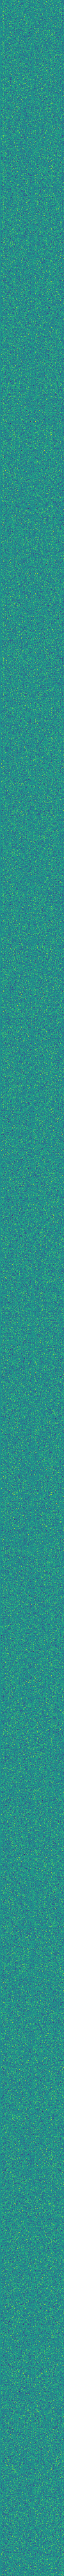
\includegraphics[interpolate=false,width=1.000000in,height=1.000000in]{antiderivative_ci_50-img0.png}}%
\end{pgfscope}%
\begin{pgfscope}%
\pgfsetbuttcap%
\pgfsetroundjoin%
\definecolor{currentfill}{rgb}{0.000000,0.000000,0.000000}%
\pgfsetfillcolor{currentfill}%
\pgfsetlinewidth{0.803000pt}%
\definecolor{currentstroke}{rgb}{0.000000,0.000000,0.000000}%
\pgfsetstrokecolor{currentstroke}%
\pgfsetdash{}{0pt}%
\pgfsys@defobject{currentmarker}{\pgfqpoint{0.000000in}{-0.048611in}}{\pgfqpoint{0.000000in}{0.000000in}}{%
\pgfpathmoveto{\pgfqpoint{0.000000in}{0.000000in}}%
\pgfpathlineto{\pgfqpoint{0.000000in}{-0.048611in}}%
\pgfusepath{stroke,fill}%
}%
\begin{pgfscope}%
\pgfsys@transformshift{0.800000in}{0.528000in}%
\pgfsys@useobject{currentmarker}{}%
\end{pgfscope}%
\end{pgfscope}%
\begin{pgfscope}%
\definecolor{textcolor}{rgb}{0.000000,0.000000,0.000000}%
\pgfsetstrokecolor{textcolor}%
\pgfsetfillcolor{textcolor}%
\pgftext[x=0.800000in,y=0.430778in,,top]{\color{textcolor}{\rmfamily\fontsize{12.000000}{14.400000}\selectfont\catcode`\^=\active\def^{\ifmmode\sp\else\^{}\fi}\catcode`\%=\active\def%{\%}0}}%
\end{pgfscope}%
\begin{pgfscope}%
\pgfsetbuttcap%
\pgfsetroundjoin%
\definecolor{currentfill}{rgb}{0.000000,0.000000,0.000000}%
\pgfsetfillcolor{currentfill}%
\pgfsetlinewidth{0.803000pt}%
\definecolor{currentstroke}{rgb}{0.000000,0.000000,0.000000}%
\pgfsetstrokecolor{currentstroke}%
\pgfsetdash{}{0pt}%
\pgfsys@defobject{currentmarker}{\pgfqpoint{0.000000in}{-0.048611in}}{\pgfqpoint{0.000000in}{0.000000in}}{%
\pgfpathmoveto{\pgfqpoint{0.000000in}{0.000000in}}%
\pgfpathlineto{\pgfqpoint{0.000000in}{-0.048611in}}%
\pgfusepath{stroke,fill}%
}%
\begin{pgfscope}%
\pgfsys@transformshift{1.593600in}{0.528000in}%
\pgfsys@useobject{currentmarker}{}%
\end{pgfscope}%
\end{pgfscope}%
\begin{pgfscope}%
\definecolor{textcolor}{rgb}{0.000000,0.000000,0.000000}%
\pgfsetstrokecolor{textcolor}%
\pgfsetfillcolor{textcolor}%
\pgftext[x=1.593600in,y=0.430778in,,top]{\color{textcolor}{\rmfamily\fontsize{12.000000}{14.400000}\selectfont\catcode`\^=\active\def^{\ifmmode\sp\else\^{}\fi}\catcode`\%=\active\def%{\%}10}}%
\end{pgfscope}%
\begin{pgfscope}%
\pgfsetbuttcap%
\pgfsetroundjoin%
\definecolor{currentfill}{rgb}{0.000000,0.000000,0.000000}%
\pgfsetfillcolor{currentfill}%
\pgfsetlinewidth{0.803000pt}%
\definecolor{currentstroke}{rgb}{0.000000,0.000000,0.000000}%
\pgfsetstrokecolor{currentstroke}%
\pgfsetdash{}{0pt}%
\pgfsys@defobject{currentmarker}{\pgfqpoint{0.000000in}{-0.048611in}}{\pgfqpoint{0.000000in}{0.000000in}}{%
\pgfpathmoveto{\pgfqpoint{0.000000in}{0.000000in}}%
\pgfpathlineto{\pgfqpoint{0.000000in}{-0.048611in}}%
\pgfusepath{stroke,fill}%
}%
\begin{pgfscope}%
\pgfsys@transformshift{2.387200in}{0.528000in}%
\pgfsys@useobject{currentmarker}{}%
\end{pgfscope}%
\end{pgfscope}%
\begin{pgfscope}%
\definecolor{textcolor}{rgb}{0.000000,0.000000,0.000000}%
\pgfsetstrokecolor{textcolor}%
\pgfsetfillcolor{textcolor}%
\pgftext[x=2.387200in,y=0.430778in,,top]{\color{textcolor}{\rmfamily\fontsize{12.000000}{14.400000}\selectfont\catcode`\^=\active\def^{\ifmmode\sp\else\^{}\fi}\catcode`\%=\active\def%{\%}20}}%
\end{pgfscope}%
\begin{pgfscope}%
\pgfsetbuttcap%
\pgfsetroundjoin%
\definecolor{currentfill}{rgb}{0.000000,0.000000,0.000000}%
\pgfsetfillcolor{currentfill}%
\pgfsetlinewidth{0.803000pt}%
\definecolor{currentstroke}{rgb}{0.000000,0.000000,0.000000}%
\pgfsetstrokecolor{currentstroke}%
\pgfsetdash{}{0pt}%
\pgfsys@defobject{currentmarker}{\pgfqpoint{0.000000in}{-0.048611in}}{\pgfqpoint{0.000000in}{0.000000in}}{%
\pgfpathmoveto{\pgfqpoint{0.000000in}{0.000000in}}%
\pgfpathlineto{\pgfqpoint{0.000000in}{-0.048611in}}%
\pgfusepath{stroke,fill}%
}%
\begin{pgfscope}%
\pgfsys@transformshift{3.180800in}{0.528000in}%
\pgfsys@useobject{currentmarker}{}%
\end{pgfscope}%
\end{pgfscope}%
\begin{pgfscope}%
\definecolor{textcolor}{rgb}{0.000000,0.000000,0.000000}%
\pgfsetstrokecolor{textcolor}%
\pgfsetfillcolor{textcolor}%
\pgftext[x=3.180800in,y=0.430778in,,top]{\color{textcolor}{\rmfamily\fontsize{12.000000}{14.400000}\selectfont\catcode`\^=\active\def^{\ifmmode\sp\else\^{}\fi}\catcode`\%=\active\def%{\%}30}}%
\end{pgfscope}%
\begin{pgfscope}%
\pgfsetbuttcap%
\pgfsetroundjoin%
\definecolor{currentfill}{rgb}{0.000000,0.000000,0.000000}%
\pgfsetfillcolor{currentfill}%
\pgfsetlinewidth{0.803000pt}%
\definecolor{currentstroke}{rgb}{0.000000,0.000000,0.000000}%
\pgfsetstrokecolor{currentstroke}%
\pgfsetdash{}{0pt}%
\pgfsys@defobject{currentmarker}{\pgfqpoint{0.000000in}{-0.048611in}}{\pgfqpoint{0.000000in}{0.000000in}}{%
\pgfpathmoveto{\pgfqpoint{0.000000in}{0.000000in}}%
\pgfpathlineto{\pgfqpoint{0.000000in}{-0.048611in}}%
\pgfusepath{stroke,fill}%
}%
\begin{pgfscope}%
\pgfsys@transformshift{3.974400in}{0.528000in}%
\pgfsys@useobject{currentmarker}{}%
\end{pgfscope}%
\end{pgfscope}%
\begin{pgfscope}%
\definecolor{textcolor}{rgb}{0.000000,0.000000,0.000000}%
\pgfsetstrokecolor{textcolor}%
\pgfsetfillcolor{textcolor}%
\pgftext[x=3.974400in,y=0.430778in,,top]{\color{textcolor}{\rmfamily\fontsize{12.000000}{14.400000}\selectfont\catcode`\^=\active\def^{\ifmmode\sp\else\^{}\fi}\catcode`\%=\active\def%{\%}40}}%
\end{pgfscope}%
\begin{pgfscope}%
\pgfsetbuttcap%
\pgfsetroundjoin%
\definecolor{currentfill}{rgb}{0.000000,0.000000,0.000000}%
\pgfsetfillcolor{currentfill}%
\pgfsetlinewidth{0.803000pt}%
\definecolor{currentstroke}{rgb}{0.000000,0.000000,0.000000}%
\pgfsetstrokecolor{currentstroke}%
\pgfsetdash{}{0pt}%
\pgfsys@defobject{currentmarker}{\pgfqpoint{0.000000in}{-0.048611in}}{\pgfqpoint{0.000000in}{0.000000in}}{%
\pgfpathmoveto{\pgfqpoint{0.000000in}{0.000000in}}%
\pgfpathlineto{\pgfqpoint{0.000000in}{-0.048611in}}%
\pgfusepath{stroke,fill}%
}%
\begin{pgfscope}%
\pgfsys@transformshift{4.768000in}{0.528000in}%
\pgfsys@useobject{currentmarker}{}%
\end{pgfscope}%
\end{pgfscope}%
\begin{pgfscope}%
\definecolor{textcolor}{rgb}{0.000000,0.000000,0.000000}%
\pgfsetstrokecolor{textcolor}%
\pgfsetfillcolor{textcolor}%
\pgftext[x=4.768000in,y=0.430778in,,top]{\color{textcolor}{\rmfamily\fontsize{12.000000}{14.400000}\selectfont\catcode`\^=\active\def^{\ifmmode\sp\else\^{}\fi}\catcode`\%=\active\def%{\%}50}}%
\end{pgfscope}%
\begin{pgfscope}%
\definecolor{textcolor}{rgb}{0.000000,0.000000,0.000000}%
\pgfsetstrokecolor{textcolor}%
\pgfsetfillcolor{textcolor}%
\pgftext[x=2.784000in,y=0.213927in,,top]{\color{textcolor}{\rmfamily\fontsize{12.000000}{14.400000}\selectfont\catcode`\^=\active\def^{\ifmmode\sp\else\^{}\fi}\catcode`\%=\active\def%{\%}input coefficients}}%
\end{pgfscope}%
\begin{pgfscope}%
\pgfsetbuttcap%
\pgfsetroundjoin%
\definecolor{currentfill}{rgb}{0.000000,0.000000,0.000000}%
\pgfsetfillcolor{currentfill}%
\pgfsetlinewidth{0.803000pt}%
\definecolor{currentstroke}{rgb}{0.000000,0.000000,0.000000}%
\pgfsetstrokecolor{currentstroke}%
\pgfsetdash{}{0pt}%
\pgfsys@defobject{currentmarker}{\pgfqpoint{-0.048611in}{0.000000in}}{\pgfqpoint{-0.000000in}{0.000000in}}{%
\pgfpathmoveto{\pgfqpoint{-0.000000in}{0.000000in}}%
\pgfpathlineto{\pgfqpoint{-0.048611in}{0.000000in}}%
\pgfusepath{stroke,fill}%
}%
\begin{pgfscope}%
\pgfsys@transformshift{0.800000in}{4.224000in}%
\pgfsys@useobject{currentmarker}{}%
\end{pgfscope}%
\end{pgfscope}%
\begin{pgfscope}%
\definecolor{textcolor}{rgb}{0.000000,0.000000,0.000000}%
\pgfsetstrokecolor{textcolor}%
\pgfsetfillcolor{textcolor}%
\pgftext[x=0.596739in, y=4.160686in, left, base]{\color{textcolor}{\rmfamily\fontsize{12.000000}{14.400000}\selectfont\catcode`\^=\active\def^{\ifmmode\sp\else\^{}\fi}\catcode`\%=\active\def%{\%}0}}%
\end{pgfscope}%
\begin{pgfscope}%
\pgfsetbuttcap%
\pgfsetroundjoin%
\definecolor{currentfill}{rgb}{0.000000,0.000000,0.000000}%
\pgfsetfillcolor{currentfill}%
\pgfsetlinewidth{0.803000pt}%
\definecolor{currentstroke}{rgb}{0.000000,0.000000,0.000000}%
\pgfsetstrokecolor{currentstroke}%
\pgfsetdash{}{0pt}%
\pgfsys@defobject{currentmarker}{\pgfqpoint{-0.048611in}{0.000000in}}{\pgfqpoint{-0.000000in}{0.000000in}}{%
\pgfpathmoveto{\pgfqpoint{-0.000000in}{0.000000in}}%
\pgfpathlineto{\pgfqpoint{-0.048611in}{0.000000in}}%
\pgfusepath{stroke,fill}%
}%
\begin{pgfscope}%
\pgfsys@transformshift{0.800000in}{3.762000in}%
\pgfsys@useobject{currentmarker}{}%
\end{pgfscope}%
\end{pgfscope}%
\begin{pgfscope}%
\definecolor{textcolor}{rgb}{0.000000,0.000000,0.000000}%
\pgfsetstrokecolor{textcolor}%
\pgfsetfillcolor{textcolor}%
\pgftext[x=0.384662in, y=3.698686in, left, base]{\color{textcolor}{\rmfamily\fontsize{12.000000}{14.400000}\selectfont\catcode`\^=\active\def^{\ifmmode\sp\else\^{}\fi}\catcode`\%=\active\def%{\%}500}}%
\end{pgfscope}%
\begin{pgfscope}%
\pgfsetbuttcap%
\pgfsetroundjoin%
\definecolor{currentfill}{rgb}{0.000000,0.000000,0.000000}%
\pgfsetfillcolor{currentfill}%
\pgfsetlinewidth{0.803000pt}%
\definecolor{currentstroke}{rgb}{0.000000,0.000000,0.000000}%
\pgfsetstrokecolor{currentstroke}%
\pgfsetdash{}{0pt}%
\pgfsys@defobject{currentmarker}{\pgfqpoint{-0.048611in}{0.000000in}}{\pgfqpoint{-0.000000in}{0.000000in}}{%
\pgfpathmoveto{\pgfqpoint{-0.000000in}{0.000000in}}%
\pgfpathlineto{\pgfqpoint{-0.048611in}{0.000000in}}%
\pgfusepath{stroke,fill}%
}%
\begin{pgfscope}%
\pgfsys@transformshift{0.800000in}{3.300000in}%
\pgfsys@useobject{currentmarker}{}%
\end{pgfscope}%
\end{pgfscope}%
\begin{pgfscope}%
\definecolor{textcolor}{rgb}{0.000000,0.000000,0.000000}%
\pgfsetstrokecolor{textcolor}%
\pgfsetfillcolor{textcolor}%
\pgftext[x=0.278624in, y=3.236686in, left, base]{\color{textcolor}{\rmfamily\fontsize{12.000000}{14.400000}\selectfont\catcode`\^=\active\def^{\ifmmode\sp\else\^{}\fi}\catcode`\%=\active\def%{\%}1000}}%
\end{pgfscope}%
\begin{pgfscope}%
\pgfsetbuttcap%
\pgfsetroundjoin%
\definecolor{currentfill}{rgb}{0.000000,0.000000,0.000000}%
\pgfsetfillcolor{currentfill}%
\pgfsetlinewidth{0.803000pt}%
\definecolor{currentstroke}{rgb}{0.000000,0.000000,0.000000}%
\pgfsetstrokecolor{currentstroke}%
\pgfsetdash{}{0pt}%
\pgfsys@defobject{currentmarker}{\pgfqpoint{-0.048611in}{0.000000in}}{\pgfqpoint{-0.000000in}{0.000000in}}{%
\pgfpathmoveto{\pgfqpoint{-0.000000in}{0.000000in}}%
\pgfpathlineto{\pgfqpoint{-0.048611in}{0.000000in}}%
\pgfusepath{stroke,fill}%
}%
\begin{pgfscope}%
\pgfsys@transformshift{0.800000in}{2.838000in}%
\pgfsys@useobject{currentmarker}{}%
\end{pgfscope}%
\end{pgfscope}%
\begin{pgfscope}%
\definecolor{textcolor}{rgb}{0.000000,0.000000,0.000000}%
\pgfsetstrokecolor{textcolor}%
\pgfsetfillcolor{textcolor}%
\pgftext[x=0.278624in, y=2.774686in, left, base]{\color{textcolor}{\rmfamily\fontsize{12.000000}{14.400000}\selectfont\catcode`\^=\active\def^{\ifmmode\sp\else\^{}\fi}\catcode`\%=\active\def%{\%}1500}}%
\end{pgfscope}%
\begin{pgfscope}%
\pgfsetbuttcap%
\pgfsetroundjoin%
\definecolor{currentfill}{rgb}{0.000000,0.000000,0.000000}%
\pgfsetfillcolor{currentfill}%
\pgfsetlinewidth{0.803000pt}%
\definecolor{currentstroke}{rgb}{0.000000,0.000000,0.000000}%
\pgfsetstrokecolor{currentstroke}%
\pgfsetdash{}{0pt}%
\pgfsys@defobject{currentmarker}{\pgfqpoint{-0.048611in}{0.000000in}}{\pgfqpoint{-0.000000in}{0.000000in}}{%
\pgfpathmoveto{\pgfqpoint{-0.000000in}{0.000000in}}%
\pgfpathlineto{\pgfqpoint{-0.048611in}{0.000000in}}%
\pgfusepath{stroke,fill}%
}%
\begin{pgfscope}%
\pgfsys@transformshift{0.800000in}{2.376000in}%
\pgfsys@useobject{currentmarker}{}%
\end{pgfscope}%
\end{pgfscope}%
\begin{pgfscope}%
\definecolor{textcolor}{rgb}{0.000000,0.000000,0.000000}%
\pgfsetstrokecolor{textcolor}%
\pgfsetfillcolor{textcolor}%
\pgftext[x=0.278624in, y=2.312686in, left, base]{\color{textcolor}{\rmfamily\fontsize{12.000000}{14.400000}\selectfont\catcode`\^=\active\def^{\ifmmode\sp\else\^{}\fi}\catcode`\%=\active\def%{\%}2000}}%
\end{pgfscope}%
\begin{pgfscope}%
\pgfsetbuttcap%
\pgfsetroundjoin%
\definecolor{currentfill}{rgb}{0.000000,0.000000,0.000000}%
\pgfsetfillcolor{currentfill}%
\pgfsetlinewidth{0.803000pt}%
\definecolor{currentstroke}{rgb}{0.000000,0.000000,0.000000}%
\pgfsetstrokecolor{currentstroke}%
\pgfsetdash{}{0pt}%
\pgfsys@defobject{currentmarker}{\pgfqpoint{-0.048611in}{0.000000in}}{\pgfqpoint{-0.000000in}{0.000000in}}{%
\pgfpathmoveto{\pgfqpoint{-0.000000in}{0.000000in}}%
\pgfpathlineto{\pgfqpoint{-0.048611in}{0.000000in}}%
\pgfusepath{stroke,fill}%
}%
\begin{pgfscope}%
\pgfsys@transformshift{0.800000in}{1.914000in}%
\pgfsys@useobject{currentmarker}{}%
\end{pgfscope}%
\end{pgfscope}%
\begin{pgfscope}%
\definecolor{textcolor}{rgb}{0.000000,0.000000,0.000000}%
\pgfsetstrokecolor{textcolor}%
\pgfsetfillcolor{textcolor}%
\pgftext[x=0.278624in, y=1.850686in, left, base]{\color{textcolor}{\rmfamily\fontsize{12.000000}{14.400000}\selectfont\catcode`\^=\active\def^{\ifmmode\sp\else\^{}\fi}\catcode`\%=\active\def%{\%}2500}}%
\end{pgfscope}%
\begin{pgfscope}%
\pgfsetbuttcap%
\pgfsetroundjoin%
\definecolor{currentfill}{rgb}{0.000000,0.000000,0.000000}%
\pgfsetfillcolor{currentfill}%
\pgfsetlinewidth{0.803000pt}%
\definecolor{currentstroke}{rgb}{0.000000,0.000000,0.000000}%
\pgfsetstrokecolor{currentstroke}%
\pgfsetdash{}{0pt}%
\pgfsys@defobject{currentmarker}{\pgfqpoint{-0.048611in}{0.000000in}}{\pgfqpoint{-0.000000in}{0.000000in}}{%
\pgfpathmoveto{\pgfqpoint{-0.000000in}{0.000000in}}%
\pgfpathlineto{\pgfqpoint{-0.048611in}{0.000000in}}%
\pgfusepath{stroke,fill}%
}%
\begin{pgfscope}%
\pgfsys@transformshift{0.800000in}{1.452000in}%
\pgfsys@useobject{currentmarker}{}%
\end{pgfscope}%
\end{pgfscope}%
\begin{pgfscope}%
\definecolor{textcolor}{rgb}{0.000000,0.000000,0.000000}%
\pgfsetstrokecolor{textcolor}%
\pgfsetfillcolor{textcolor}%
\pgftext[x=0.278624in, y=1.388686in, left, base]{\color{textcolor}{\rmfamily\fontsize{12.000000}{14.400000}\selectfont\catcode`\^=\active\def^{\ifmmode\sp\else\^{}\fi}\catcode`\%=\active\def%{\%}3000}}%
\end{pgfscope}%
\begin{pgfscope}%
\pgfsetbuttcap%
\pgfsetroundjoin%
\definecolor{currentfill}{rgb}{0.000000,0.000000,0.000000}%
\pgfsetfillcolor{currentfill}%
\pgfsetlinewidth{0.803000pt}%
\definecolor{currentstroke}{rgb}{0.000000,0.000000,0.000000}%
\pgfsetstrokecolor{currentstroke}%
\pgfsetdash{}{0pt}%
\pgfsys@defobject{currentmarker}{\pgfqpoint{-0.048611in}{0.000000in}}{\pgfqpoint{-0.000000in}{0.000000in}}{%
\pgfpathmoveto{\pgfqpoint{-0.000000in}{0.000000in}}%
\pgfpathlineto{\pgfqpoint{-0.048611in}{0.000000in}}%
\pgfusepath{stroke,fill}%
}%
\begin{pgfscope}%
\pgfsys@transformshift{0.800000in}{0.990000in}%
\pgfsys@useobject{currentmarker}{}%
\end{pgfscope}%
\end{pgfscope}%
\begin{pgfscope}%
\definecolor{textcolor}{rgb}{0.000000,0.000000,0.000000}%
\pgfsetstrokecolor{textcolor}%
\pgfsetfillcolor{textcolor}%
\pgftext[x=0.278624in, y=0.926686in, left, base]{\color{textcolor}{\rmfamily\fontsize{12.000000}{14.400000}\selectfont\catcode`\^=\active\def^{\ifmmode\sp\else\^{}\fi}\catcode`\%=\active\def%{\%}3500}}%
\end{pgfscope}%
\begin{pgfscope}%
\pgfsetbuttcap%
\pgfsetroundjoin%
\definecolor{currentfill}{rgb}{0.000000,0.000000,0.000000}%
\pgfsetfillcolor{currentfill}%
\pgfsetlinewidth{0.803000pt}%
\definecolor{currentstroke}{rgb}{0.000000,0.000000,0.000000}%
\pgfsetstrokecolor{currentstroke}%
\pgfsetdash{}{0pt}%
\pgfsys@defobject{currentmarker}{\pgfqpoint{-0.048611in}{0.000000in}}{\pgfqpoint{-0.000000in}{0.000000in}}{%
\pgfpathmoveto{\pgfqpoint{-0.000000in}{0.000000in}}%
\pgfpathlineto{\pgfqpoint{-0.048611in}{0.000000in}}%
\pgfusepath{stroke,fill}%
}%
\begin{pgfscope}%
\pgfsys@transformshift{0.800000in}{0.528000in}%
\pgfsys@useobject{currentmarker}{}%
\end{pgfscope}%
\end{pgfscope}%
\begin{pgfscope}%
\definecolor{textcolor}{rgb}{0.000000,0.000000,0.000000}%
\pgfsetstrokecolor{textcolor}%
\pgfsetfillcolor{textcolor}%
\pgftext[x=0.278624in, y=0.464686in, left, base]{\color{textcolor}{\rmfamily\fontsize{12.000000}{14.400000}\selectfont\catcode`\^=\active\def^{\ifmmode\sp\else\^{}\fi}\catcode`\%=\active\def%{\%}4000}}%
\end{pgfscope}%
\begin{pgfscope}%
\definecolor{textcolor}{rgb}{0.000000,0.000000,0.000000}%
\pgfsetstrokecolor{textcolor}%
\pgfsetfillcolor{textcolor}%
\pgftext[x=0.223069in,y=2.376000in,,bottom,rotate=90.000000]{\color{textcolor}{\rmfamily\fontsize{12.000000}{14.400000}\selectfont\catcode`\^=\active\def^{\ifmmode\sp\else\^{}\fi}\catcode`\%=\active\def%{\%}samples}}%
\end{pgfscope}%
\begin{pgfscope}%
\pgfsetrectcap%
\pgfsetmiterjoin%
\pgfsetlinewidth{0.803000pt}%
\definecolor{currentstroke}{rgb}{0.000000,0.000000,0.000000}%
\pgfsetstrokecolor{currentstroke}%
\pgfsetdash{}{0pt}%
\pgfpathmoveto{\pgfqpoint{0.800000in}{0.528000in}}%
\pgfpathlineto{\pgfqpoint{0.800000in}{4.224000in}}%
\pgfusepath{stroke}%
\end{pgfscope}%
\begin{pgfscope}%
\pgfsetrectcap%
\pgfsetmiterjoin%
\pgfsetlinewidth{0.803000pt}%
\definecolor{currentstroke}{rgb}{0.000000,0.000000,0.000000}%
\pgfsetstrokecolor{currentstroke}%
\pgfsetdash{}{0pt}%
\pgfpathmoveto{\pgfqpoint{4.768000in}{0.528000in}}%
\pgfpathlineto{\pgfqpoint{4.768000in}{4.224000in}}%
\pgfusepath{stroke}%
\end{pgfscope}%
\begin{pgfscope}%
\pgfsetrectcap%
\pgfsetmiterjoin%
\pgfsetlinewidth{0.803000pt}%
\definecolor{currentstroke}{rgb}{0.000000,0.000000,0.000000}%
\pgfsetstrokecolor{currentstroke}%
\pgfsetdash{}{0pt}%
\pgfpathmoveto{\pgfqpoint{0.800000in}{0.528000in}}%
\pgfpathlineto{\pgfqpoint{4.768000in}{0.528000in}}%
\pgfusepath{stroke}%
\end{pgfscope}%
\begin{pgfscope}%
\pgfsetrectcap%
\pgfsetmiterjoin%
\pgfsetlinewidth{0.803000pt}%
\definecolor{currentstroke}{rgb}{0.000000,0.000000,0.000000}%
\pgfsetstrokecolor{currentstroke}%
\pgfsetdash{}{0pt}%
\pgfpathmoveto{\pgfqpoint{0.800000in}{4.224000in}}%
\pgfpathlineto{\pgfqpoint{4.768000in}{4.224000in}}%
\pgfusepath{stroke}%
\end{pgfscope}%
\begin{pgfscope}%
\pgfsetbuttcap%
\pgfsetmiterjoin%
\pgfsetlinewidth{0.000000pt}%
\definecolor{currentstroke}{rgb}{0.000000,0.000000,0.000000}%
\pgfsetstrokecolor{currentstroke}%
\pgfsetstrokeopacity{0.000000}%
\pgfsetdash{}{0pt}%
\pgfpathmoveto{\pgfqpoint{5.016000in}{0.528000in}}%
\pgfpathlineto{\pgfqpoint{5.200800in}{0.528000in}}%
\pgfpathlineto{\pgfqpoint{5.200800in}{4.224000in}}%
\pgfpathlineto{\pgfqpoint{5.016000in}{4.224000in}}%
\pgfpathlineto{\pgfqpoint{5.016000in}{0.528000in}}%
\pgfpathclose%
\pgfusepath{}%
\end{pgfscope}%
\begin{pgfscope}%
\pgfsys@transformshift{5.020000in}{0.530000in}%
\pgftext[left,bottom]{
\includegraphics[interpolate=true,width=0.180000in,height=3.690000in]{antiderivative_ci_50-img1.png}}%
\end{pgfscope}%
\begin{pgfscope}%
\pgfsetbuttcap%
\pgfsetroundjoin%
\definecolor{currentfill}{rgb}{0.000000,0.000000,0.000000}%
\pgfsetfillcolor{currentfill}%
\pgfsetlinewidth{0.803000pt}%
\definecolor{currentstroke}{rgb}{0.000000,0.000000,0.000000}%
\pgfsetstrokecolor{currentstroke}%
\pgfsetdash{}{0pt}%
\pgfsys@defobject{currentmarker}{\pgfqpoint{0.000000in}{0.000000in}}{\pgfqpoint{0.048611in}{0.000000in}}{%
\pgfpathmoveto{\pgfqpoint{0.000000in}{0.000000in}}%
\pgfpathlineto{\pgfqpoint{0.048611in}{0.000000in}}%
\pgfusepath{stroke,fill}%
}%
\begin{pgfscope}%
\pgfsys@transformshift{5.200800in}{0.540424in}%
\pgfsys@useobject{currentmarker}{}%
\end{pgfscope}%
\end{pgfscope}%
\begin{pgfscope}%
\definecolor{textcolor}{rgb}{0.000000,0.000000,0.000000}%
\pgfsetstrokecolor{textcolor}%
\pgfsetfillcolor{textcolor}%
\pgftext[x=5.298022in, y=0.477110in, left, base]{\color{textcolor}{\rmfamily\fontsize{12.000000}{14.400000}\selectfont\catcode`\^=\active\def^{\ifmmode\sp\else\^{}\fi}\catcode`\%=\active\def%{\%}\ensuremath{-}100}}%
\end{pgfscope}%
\begin{pgfscope}%
\pgfsetbuttcap%
\pgfsetroundjoin%
\definecolor{currentfill}{rgb}{0.000000,0.000000,0.000000}%
\pgfsetfillcolor{currentfill}%
\pgfsetlinewidth{0.803000pt}%
\definecolor{currentstroke}{rgb}{0.000000,0.000000,0.000000}%
\pgfsetstrokecolor{currentstroke}%
\pgfsetdash{}{0pt}%
\pgfsys@defobject{currentmarker}{\pgfqpoint{0.000000in}{0.000000in}}{\pgfqpoint{0.048611in}{0.000000in}}{%
\pgfpathmoveto{\pgfqpoint{0.000000in}{0.000000in}}%
\pgfpathlineto{\pgfqpoint{0.048611in}{0.000000in}}%
\pgfusepath{stroke,fill}%
}%
\begin{pgfscope}%
\pgfsys@transformshift{5.200800in}{0.999318in}%
\pgfsys@useobject{currentmarker}{}%
\end{pgfscope}%
\end{pgfscope}%
\begin{pgfscope}%
\definecolor{textcolor}{rgb}{0.000000,0.000000,0.000000}%
\pgfsetstrokecolor{textcolor}%
\pgfsetfillcolor{textcolor}%
\pgftext[x=5.298022in, y=0.936004in, left, base]{\color{textcolor}{\rmfamily\fontsize{12.000000}{14.400000}\selectfont\catcode`\^=\active\def^{\ifmmode\sp\else\^{}\fi}\catcode`\%=\active\def%{\%}\ensuremath{-}75}}%
\end{pgfscope}%
\begin{pgfscope}%
\pgfsetbuttcap%
\pgfsetroundjoin%
\definecolor{currentfill}{rgb}{0.000000,0.000000,0.000000}%
\pgfsetfillcolor{currentfill}%
\pgfsetlinewidth{0.803000pt}%
\definecolor{currentstroke}{rgb}{0.000000,0.000000,0.000000}%
\pgfsetstrokecolor{currentstroke}%
\pgfsetdash{}{0pt}%
\pgfsys@defobject{currentmarker}{\pgfqpoint{0.000000in}{0.000000in}}{\pgfqpoint{0.048611in}{0.000000in}}{%
\pgfpathmoveto{\pgfqpoint{0.000000in}{0.000000in}}%
\pgfpathlineto{\pgfqpoint{0.048611in}{0.000000in}}%
\pgfusepath{stroke,fill}%
}%
\begin{pgfscope}%
\pgfsys@transformshift{5.200800in}{1.458212in}%
\pgfsys@useobject{currentmarker}{}%
\end{pgfscope}%
\end{pgfscope}%
\begin{pgfscope}%
\definecolor{textcolor}{rgb}{0.000000,0.000000,0.000000}%
\pgfsetstrokecolor{textcolor}%
\pgfsetfillcolor{textcolor}%
\pgftext[x=5.298022in, y=1.394898in, left, base]{\color{textcolor}{\rmfamily\fontsize{12.000000}{14.400000}\selectfont\catcode`\^=\active\def^{\ifmmode\sp\else\^{}\fi}\catcode`\%=\active\def%{\%}\ensuremath{-}50}}%
\end{pgfscope}%
\begin{pgfscope}%
\pgfsetbuttcap%
\pgfsetroundjoin%
\definecolor{currentfill}{rgb}{0.000000,0.000000,0.000000}%
\pgfsetfillcolor{currentfill}%
\pgfsetlinewidth{0.803000pt}%
\definecolor{currentstroke}{rgb}{0.000000,0.000000,0.000000}%
\pgfsetstrokecolor{currentstroke}%
\pgfsetdash{}{0pt}%
\pgfsys@defobject{currentmarker}{\pgfqpoint{0.000000in}{0.000000in}}{\pgfqpoint{0.048611in}{0.000000in}}{%
\pgfpathmoveto{\pgfqpoint{0.000000in}{0.000000in}}%
\pgfpathlineto{\pgfqpoint{0.048611in}{0.000000in}}%
\pgfusepath{stroke,fill}%
}%
\begin{pgfscope}%
\pgfsys@transformshift{5.200800in}{1.917106in}%
\pgfsys@useobject{currentmarker}{}%
\end{pgfscope}%
\end{pgfscope}%
\begin{pgfscope}%
\definecolor{textcolor}{rgb}{0.000000,0.000000,0.000000}%
\pgfsetstrokecolor{textcolor}%
\pgfsetfillcolor{textcolor}%
\pgftext[x=5.298022in, y=1.853792in, left, base]{\color{textcolor}{\rmfamily\fontsize{12.000000}{14.400000}\selectfont\catcode`\^=\active\def^{\ifmmode\sp\else\^{}\fi}\catcode`\%=\active\def%{\%}\ensuremath{-}25}}%
\end{pgfscope}%
\begin{pgfscope}%
\pgfsetbuttcap%
\pgfsetroundjoin%
\definecolor{currentfill}{rgb}{0.000000,0.000000,0.000000}%
\pgfsetfillcolor{currentfill}%
\pgfsetlinewidth{0.803000pt}%
\definecolor{currentstroke}{rgb}{0.000000,0.000000,0.000000}%
\pgfsetstrokecolor{currentstroke}%
\pgfsetdash{}{0pt}%
\pgfsys@defobject{currentmarker}{\pgfqpoint{0.000000in}{0.000000in}}{\pgfqpoint{0.048611in}{0.000000in}}{%
\pgfpathmoveto{\pgfqpoint{0.000000in}{0.000000in}}%
\pgfpathlineto{\pgfqpoint{0.048611in}{0.000000in}}%
\pgfusepath{stroke,fill}%
}%
\begin{pgfscope}%
\pgfsys@transformshift{5.200800in}{2.376000in}%
\pgfsys@useobject{currentmarker}{}%
\end{pgfscope}%
\end{pgfscope}%
\begin{pgfscope}%
\definecolor{textcolor}{rgb}{0.000000,0.000000,0.000000}%
\pgfsetstrokecolor{textcolor}%
\pgfsetfillcolor{textcolor}%
\pgftext[x=5.298022in, y=2.312686in, left, base]{\color{textcolor}{\rmfamily\fontsize{12.000000}{14.400000}\selectfont\catcode`\^=\active\def^{\ifmmode\sp\else\^{}\fi}\catcode`\%=\active\def%{\%}0}}%
\end{pgfscope}%
\begin{pgfscope}%
\pgfsetbuttcap%
\pgfsetroundjoin%
\definecolor{currentfill}{rgb}{0.000000,0.000000,0.000000}%
\pgfsetfillcolor{currentfill}%
\pgfsetlinewidth{0.803000pt}%
\definecolor{currentstroke}{rgb}{0.000000,0.000000,0.000000}%
\pgfsetstrokecolor{currentstroke}%
\pgfsetdash{}{0pt}%
\pgfsys@defobject{currentmarker}{\pgfqpoint{0.000000in}{0.000000in}}{\pgfqpoint{0.048611in}{0.000000in}}{%
\pgfpathmoveto{\pgfqpoint{0.000000in}{0.000000in}}%
\pgfpathlineto{\pgfqpoint{0.048611in}{0.000000in}}%
\pgfusepath{stroke,fill}%
}%
\begin{pgfscope}%
\pgfsys@transformshift{5.200800in}{2.834894in}%
\pgfsys@useobject{currentmarker}{}%
\end{pgfscope}%
\end{pgfscope}%
\begin{pgfscope}%
\definecolor{textcolor}{rgb}{0.000000,0.000000,0.000000}%
\pgfsetstrokecolor{textcolor}%
\pgfsetfillcolor{textcolor}%
\pgftext[x=5.298022in, y=2.771580in, left, base]{\color{textcolor}{\rmfamily\fontsize{12.000000}{14.400000}\selectfont\catcode`\^=\active\def^{\ifmmode\sp\else\^{}\fi}\catcode`\%=\active\def%{\%}25}}%
\end{pgfscope}%
\begin{pgfscope}%
\pgfsetbuttcap%
\pgfsetroundjoin%
\definecolor{currentfill}{rgb}{0.000000,0.000000,0.000000}%
\pgfsetfillcolor{currentfill}%
\pgfsetlinewidth{0.803000pt}%
\definecolor{currentstroke}{rgb}{0.000000,0.000000,0.000000}%
\pgfsetstrokecolor{currentstroke}%
\pgfsetdash{}{0pt}%
\pgfsys@defobject{currentmarker}{\pgfqpoint{0.000000in}{0.000000in}}{\pgfqpoint{0.048611in}{0.000000in}}{%
\pgfpathmoveto{\pgfqpoint{0.000000in}{0.000000in}}%
\pgfpathlineto{\pgfqpoint{0.048611in}{0.000000in}}%
\pgfusepath{stroke,fill}%
}%
\begin{pgfscope}%
\pgfsys@transformshift{5.200800in}{3.293788in}%
\pgfsys@useobject{currentmarker}{}%
\end{pgfscope}%
\end{pgfscope}%
\begin{pgfscope}%
\definecolor{textcolor}{rgb}{0.000000,0.000000,0.000000}%
\pgfsetstrokecolor{textcolor}%
\pgfsetfillcolor{textcolor}%
\pgftext[x=5.298022in, y=3.230474in, left, base]{\color{textcolor}{\rmfamily\fontsize{12.000000}{14.400000}\selectfont\catcode`\^=\active\def^{\ifmmode\sp\else\^{}\fi}\catcode`\%=\active\def%{\%}50}}%
\end{pgfscope}%
\begin{pgfscope}%
\pgfsetbuttcap%
\pgfsetroundjoin%
\definecolor{currentfill}{rgb}{0.000000,0.000000,0.000000}%
\pgfsetfillcolor{currentfill}%
\pgfsetlinewidth{0.803000pt}%
\definecolor{currentstroke}{rgb}{0.000000,0.000000,0.000000}%
\pgfsetstrokecolor{currentstroke}%
\pgfsetdash{}{0pt}%
\pgfsys@defobject{currentmarker}{\pgfqpoint{0.000000in}{0.000000in}}{\pgfqpoint{0.048611in}{0.000000in}}{%
\pgfpathmoveto{\pgfqpoint{0.000000in}{0.000000in}}%
\pgfpathlineto{\pgfqpoint{0.048611in}{0.000000in}}%
\pgfusepath{stroke,fill}%
}%
\begin{pgfscope}%
\pgfsys@transformshift{5.200800in}{3.752682in}%
\pgfsys@useobject{currentmarker}{}%
\end{pgfscope}%
\end{pgfscope}%
\begin{pgfscope}%
\definecolor{textcolor}{rgb}{0.000000,0.000000,0.000000}%
\pgfsetstrokecolor{textcolor}%
\pgfsetfillcolor{textcolor}%
\pgftext[x=5.298022in, y=3.689368in, left, base]{\color{textcolor}{\rmfamily\fontsize{12.000000}{14.400000}\selectfont\catcode`\^=\active\def^{\ifmmode\sp\else\^{}\fi}\catcode`\%=\active\def%{\%}75}}%
\end{pgfscope}%
\begin{pgfscope}%
\pgfsetbuttcap%
\pgfsetroundjoin%
\definecolor{currentfill}{rgb}{0.000000,0.000000,0.000000}%
\pgfsetfillcolor{currentfill}%
\pgfsetlinewidth{0.803000pt}%
\definecolor{currentstroke}{rgb}{0.000000,0.000000,0.000000}%
\pgfsetstrokecolor{currentstroke}%
\pgfsetdash{}{0pt}%
\pgfsys@defobject{currentmarker}{\pgfqpoint{0.000000in}{0.000000in}}{\pgfqpoint{0.048611in}{0.000000in}}{%
\pgfpathmoveto{\pgfqpoint{0.000000in}{0.000000in}}%
\pgfpathlineto{\pgfqpoint{0.048611in}{0.000000in}}%
\pgfusepath{stroke,fill}%
}%
\begin{pgfscope}%
\pgfsys@transformshift{5.200800in}{4.211576in}%
\pgfsys@useobject{currentmarker}{}%
\end{pgfscope}%
\end{pgfscope}%
\begin{pgfscope}%
\definecolor{textcolor}{rgb}{0.000000,0.000000,0.000000}%
\pgfsetstrokecolor{textcolor}%
\pgfsetfillcolor{textcolor}%
\pgftext[x=5.298022in, y=4.148262in, left, base]{\color{textcolor}{\rmfamily\fontsize{12.000000}{14.400000}\selectfont\catcode`\^=\active\def^{\ifmmode\sp\else\^{}\fi}\catcode`\%=\active\def%{\%}100}}%
\end{pgfscope}%
\begin{pgfscope}%
\pgfsetrectcap%
\pgfsetmiterjoin%
\pgfsetlinewidth{0.803000pt}%
\definecolor{currentstroke}{rgb}{0.000000,0.000000,0.000000}%
\pgfsetstrokecolor{currentstroke}%
\pgfsetdash{}{0pt}%
\pgfpathmoveto{\pgfqpoint{5.016000in}{0.528000in}}%
\pgfpathlineto{\pgfqpoint{5.108400in}{0.528000in}}%
\pgfpathlineto{\pgfqpoint{5.200800in}{0.528000in}}%
\pgfpathlineto{\pgfqpoint{5.200800in}{4.224000in}}%
\pgfpathlineto{\pgfqpoint{5.108400in}{4.224000in}}%
\pgfpathlineto{\pgfqpoint{5.016000in}{4.224000in}}%
\pgfpathlineto{\pgfqpoint{5.016000in}{0.528000in}}%
\pgfpathclose%
\pgfusepath{stroke}%
\end{pgfscope}%
\end{pgfpicture}%
\makeatother%
\endgroup%

      \end{adjustbox}
      \caption{Correlation image 50\% noise.}\label{fig:sc1_ci_50}
    \end{subfigure}
    \begin{subfigure}{0.49\linewidth}
      \begin{adjustbox}{width=\linewidth}
        \begingroup%
\makeatletter%
\begin{pgfpicture}%
\pgfpathrectangle{\pgfpointorigin}{\pgfqpoint{4.000000in}{3.000000in}}%
\pgfusepath{use as bounding box, clip}%
\begin{pgfscope}%
\pgfsetbuttcap%
\pgfsetmiterjoin%
\pgfsetlinewidth{0.000000pt}%
\definecolor{currentstroke}{rgb}{0.000000,0.000000,0.000000}%
\pgfsetstrokecolor{currentstroke}%
\pgfsetstrokeopacity{0.000000}%
\pgfsetdash{}{0pt}%
\pgfpathmoveto{\pgfqpoint{0.000000in}{0.000000in}}%
\pgfpathlineto{\pgfqpoint{4.000000in}{0.000000in}}%
\pgfpathlineto{\pgfqpoint{4.000000in}{3.000000in}}%
\pgfpathlineto{\pgfqpoint{0.000000in}{3.000000in}}%
\pgfpathlineto{\pgfqpoint{0.000000in}{0.000000in}}%
\pgfpathclose%
\pgfusepath{}%
\end{pgfscope}%
\begin{pgfscope}%
\pgfsetbuttcap%
\pgfsetmiterjoin%
\pgfsetlinewidth{0.000000pt}%
\definecolor{currentstroke}{rgb}{0.000000,0.000000,0.000000}%
\pgfsetstrokecolor{currentstroke}%
\pgfsetstrokeopacity{0.000000}%
\pgfsetdash{}{0pt}%
\pgfpathmoveto{\pgfqpoint{0.642156in}{0.517039in}}%
\pgfpathlineto{\pgfqpoint{3.032083in}{0.517039in}}%
\pgfpathlineto{\pgfqpoint{3.032083in}{2.906966in}}%
\pgfpathlineto{\pgfqpoint{0.642156in}{2.906966in}}%
\pgfpathlineto{\pgfqpoint{0.642156in}{0.517039in}}%
\pgfpathclose%
\pgfusepath{}%
\end{pgfscope}%
\begin{pgfscope}%
\pgfpathrectangle{\pgfqpoint{0.642156in}{0.517039in}}{\pgfqpoint{2.389927in}{2.389927in}}%
\pgfusepath{clip}%
\pgfsys@transformcm{2.389927}{0.000000}{0.000000}{-2.389927}{0.642156in}{2.906966in}%
\pgftext[left,bottom]{
\includegraphics[interpolate=false,width=1.000000in,height=1.000000in]{antiderivative_pm_50-img0.png}}%
\end{pgfscope}%
\begin{pgfscope}%
\pgfsetbuttcap%
\pgfsetroundjoin%
\definecolor{currentfill}{rgb}{0.000000,0.000000,0.000000}%
\pgfsetfillcolor{currentfill}%
\pgfsetlinewidth{0.803000pt}%
\definecolor{currentstroke}{rgb}{0.000000,0.000000,0.000000}%
\pgfsetstrokecolor{currentstroke}%
\pgfsetdash{}{0pt}%
\pgfsys@defobject{currentmarker}{\pgfqpoint{0.000000in}{-0.048611in}}{\pgfqpoint{0.000000in}{0.000000in}}{%
\pgfpathmoveto{\pgfqpoint{0.000000in}{0.000000in}}%
\pgfpathlineto{\pgfqpoint{0.000000in}{-0.048611in}}%
\pgfusepath{stroke,fill}%
}%
\begin{pgfscope}%
\pgfsys@transformshift{0.654106in}{0.517039in}%
\pgfsys@useobject{currentmarker}{}%
\end{pgfscope}%
\end{pgfscope}%
\begin{pgfscope}%
\definecolor{textcolor}{rgb}{0.000000,0.000000,0.000000}%
\pgfsetstrokecolor{textcolor}%
\pgfsetfillcolor{textcolor}%
\pgftext[x=0.654106in,y=0.419816in,,top]{\color{textcolor}{\rmfamily\fontsize{12.000000}{14.400000}\selectfont\catcode`\^=\active\def^{\ifmmode\sp\else\^{}\fi}\catcode`\%=\active\def%{\%}0}}%
\end{pgfscope}%
\begin{pgfscope}%
\pgfsetbuttcap%
\pgfsetroundjoin%
\definecolor{currentfill}{rgb}{0.000000,0.000000,0.000000}%
\pgfsetfillcolor{currentfill}%
\pgfsetlinewidth{0.803000pt}%
\definecolor{currentstroke}{rgb}{0.000000,0.000000,0.000000}%
\pgfsetstrokecolor{currentstroke}%
\pgfsetdash{}{0pt}%
\pgfsys@defobject{currentmarker}{\pgfqpoint{0.000000in}{-0.048611in}}{\pgfqpoint{0.000000in}{0.000000in}}{%
\pgfpathmoveto{\pgfqpoint{0.000000in}{0.000000in}}%
\pgfpathlineto{\pgfqpoint{0.000000in}{-0.048611in}}%
\pgfusepath{stroke,fill}%
}%
\begin{pgfscope}%
\pgfsys@transformshift{1.251588in}{0.517039in}%
\pgfsys@useobject{currentmarker}{}%
\end{pgfscope}%
\end{pgfscope}%
\begin{pgfscope}%
\definecolor{textcolor}{rgb}{0.000000,0.000000,0.000000}%
\pgfsetstrokecolor{textcolor}%
\pgfsetfillcolor{textcolor}%
\pgftext[x=1.251588in,y=0.419816in,,top]{\color{textcolor}{\rmfamily\fontsize{12.000000}{14.400000}\selectfont\catcode`\^=\active\def^{\ifmmode\sp\else\^{}\fi}\catcode`\%=\active\def%{\%}25}}%
\end{pgfscope}%
\begin{pgfscope}%
\pgfsetbuttcap%
\pgfsetroundjoin%
\definecolor{currentfill}{rgb}{0.000000,0.000000,0.000000}%
\pgfsetfillcolor{currentfill}%
\pgfsetlinewidth{0.803000pt}%
\definecolor{currentstroke}{rgb}{0.000000,0.000000,0.000000}%
\pgfsetstrokecolor{currentstroke}%
\pgfsetdash{}{0pt}%
\pgfsys@defobject{currentmarker}{\pgfqpoint{0.000000in}{-0.048611in}}{\pgfqpoint{0.000000in}{0.000000in}}{%
\pgfpathmoveto{\pgfqpoint{0.000000in}{0.000000in}}%
\pgfpathlineto{\pgfqpoint{0.000000in}{-0.048611in}}%
\pgfusepath{stroke,fill}%
}%
\begin{pgfscope}%
\pgfsys@transformshift{1.849069in}{0.517039in}%
\pgfsys@useobject{currentmarker}{}%
\end{pgfscope}%
\end{pgfscope}%
\begin{pgfscope}%
\definecolor{textcolor}{rgb}{0.000000,0.000000,0.000000}%
\pgfsetstrokecolor{textcolor}%
\pgfsetfillcolor{textcolor}%
\pgftext[x=1.849069in,y=0.419816in,,top]{\color{textcolor}{\rmfamily\fontsize{12.000000}{14.400000}\selectfont\catcode`\^=\active\def^{\ifmmode\sp\else\^{}\fi}\catcode`\%=\active\def%{\%}50}}%
\end{pgfscope}%
\begin{pgfscope}%
\pgfsetbuttcap%
\pgfsetroundjoin%
\definecolor{currentfill}{rgb}{0.000000,0.000000,0.000000}%
\pgfsetfillcolor{currentfill}%
\pgfsetlinewidth{0.803000pt}%
\definecolor{currentstroke}{rgb}{0.000000,0.000000,0.000000}%
\pgfsetstrokecolor{currentstroke}%
\pgfsetdash{}{0pt}%
\pgfsys@defobject{currentmarker}{\pgfqpoint{0.000000in}{-0.048611in}}{\pgfqpoint{0.000000in}{0.000000in}}{%
\pgfpathmoveto{\pgfqpoint{0.000000in}{0.000000in}}%
\pgfpathlineto{\pgfqpoint{0.000000in}{-0.048611in}}%
\pgfusepath{stroke,fill}%
}%
\begin{pgfscope}%
\pgfsys@transformshift{2.446551in}{0.517039in}%
\pgfsys@useobject{currentmarker}{}%
\end{pgfscope}%
\end{pgfscope}%
\begin{pgfscope}%
\definecolor{textcolor}{rgb}{0.000000,0.000000,0.000000}%
\pgfsetstrokecolor{textcolor}%
\pgfsetfillcolor{textcolor}%
\pgftext[x=2.446551in,y=0.419816in,,top]{\color{textcolor}{\rmfamily\fontsize{12.000000}{14.400000}\selectfont\catcode`\^=\active\def^{\ifmmode\sp\else\^{}\fi}\catcode`\%=\active\def%{\%}75}}%
\end{pgfscope}%
\begin{pgfscope}%
\definecolor{textcolor}{rgb}{0.000000,0.000000,0.000000}%
\pgfsetstrokecolor{textcolor}%
\pgfsetfillcolor{textcolor}%
\pgftext[x=1.837120in,y=0.202965in,,top]{\color{textcolor}{\rmfamily\fontsize{12.000000}{14.400000}\selectfont\catcode`\^=\active\def^{\ifmmode\sp\else\^{}\fi}\catcode`\%=\active\def%{\%}output coefficients}}%
\end{pgfscope}%
\begin{pgfscope}%
\pgfsetbuttcap%
\pgfsetroundjoin%
\definecolor{currentfill}{rgb}{0.000000,0.000000,0.000000}%
\pgfsetfillcolor{currentfill}%
\pgfsetlinewidth{0.803000pt}%
\definecolor{currentstroke}{rgb}{0.000000,0.000000,0.000000}%
\pgfsetstrokecolor{currentstroke}%
\pgfsetdash{}{0pt}%
\pgfsys@defobject{currentmarker}{\pgfqpoint{-0.048611in}{0.000000in}}{\pgfqpoint{-0.000000in}{0.000000in}}{%
\pgfpathmoveto{\pgfqpoint{-0.000000in}{0.000000in}}%
\pgfpathlineto{\pgfqpoint{-0.048611in}{0.000000in}}%
\pgfusepath{stroke,fill}%
}%
\begin{pgfscope}%
\pgfsys@transformshift{0.642156in}{2.895016in}%
\pgfsys@useobject{currentmarker}{}%
\end{pgfscope}%
\end{pgfscope}%
\begin{pgfscope}%
\definecolor{textcolor}{rgb}{0.000000,0.000000,0.000000}%
\pgfsetstrokecolor{textcolor}%
\pgfsetfillcolor{textcolor}%
\pgftext[x=0.438896in, y=2.831702in, left, base]{\color{textcolor}{\rmfamily\fontsize{12.000000}{14.400000}\selectfont\catcode`\^=\active\def^{\ifmmode\sp\else\^{}\fi}\catcode`\%=\active\def%{\%}0}}%
\end{pgfscope}%
\begin{pgfscope}%
\pgfsetbuttcap%
\pgfsetroundjoin%
\definecolor{currentfill}{rgb}{0.000000,0.000000,0.000000}%
\pgfsetfillcolor{currentfill}%
\pgfsetlinewidth{0.803000pt}%
\definecolor{currentstroke}{rgb}{0.000000,0.000000,0.000000}%
\pgfsetstrokecolor{currentstroke}%
\pgfsetdash{}{0pt}%
\pgfsys@defobject{currentmarker}{\pgfqpoint{-0.048611in}{0.000000in}}{\pgfqpoint{-0.000000in}{0.000000in}}{%
\pgfpathmoveto{\pgfqpoint{-0.000000in}{0.000000in}}%
\pgfpathlineto{\pgfqpoint{-0.048611in}{0.000000in}}%
\pgfusepath{stroke,fill}%
}%
\begin{pgfscope}%
\pgfsys@transformshift{0.642156in}{2.417031in}%
\pgfsys@useobject{currentmarker}{}%
\end{pgfscope}%
\end{pgfscope}%
\begin{pgfscope}%
\definecolor{textcolor}{rgb}{0.000000,0.000000,0.000000}%
\pgfsetstrokecolor{textcolor}%
\pgfsetfillcolor{textcolor}%
\pgftext[x=0.332857in, y=2.353717in, left, base]{\color{textcolor}{\rmfamily\fontsize{12.000000}{14.400000}\selectfont\catcode`\^=\active\def^{\ifmmode\sp\else\^{}\fi}\catcode`\%=\active\def%{\%}20}}%
\end{pgfscope}%
\begin{pgfscope}%
\pgfsetbuttcap%
\pgfsetroundjoin%
\definecolor{currentfill}{rgb}{0.000000,0.000000,0.000000}%
\pgfsetfillcolor{currentfill}%
\pgfsetlinewidth{0.803000pt}%
\definecolor{currentstroke}{rgb}{0.000000,0.000000,0.000000}%
\pgfsetstrokecolor{currentstroke}%
\pgfsetdash{}{0pt}%
\pgfsys@defobject{currentmarker}{\pgfqpoint{-0.048611in}{0.000000in}}{\pgfqpoint{-0.000000in}{0.000000in}}{%
\pgfpathmoveto{\pgfqpoint{-0.000000in}{0.000000in}}%
\pgfpathlineto{\pgfqpoint{-0.048611in}{0.000000in}}%
\pgfusepath{stroke,fill}%
}%
\begin{pgfscope}%
\pgfsys@transformshift{0.642156in}{1.939045in}%
\pgfsys@useobject{currentmarker}{}%
\end{pgfscope}%
\end{pgfscope}%
\begin{pgfscope}%
\definecolor{textcolor}{rgb}{0.000000,0.000000,0.000000}%
\pgfsetstrokecolor{textcolor}%
\pgfsetfillcolor{textcolor}%
\pgftext[x=0.332857in, y=1.875731in, left, base]{\color{textcolor}{\rmfamily\fontsize{12.000000}{14.400000}\selectfont\catcode`\^=\active\def^{\ifmmode\sp\else\^{}\fi}\catcode`\%=\active\def%{\%}40}}%
\end{pgfscope}%
\begin{pgfscope}%
\pgfsetbuttcap%
\pgfsetroundjoin%
\definecolor{currentfill}{rgb}{0.000000,0.000000,0.000000}%
\pgfsetfillcolor{currentfill}%
\pgfsetlinewidth{0.803000pt}%
\definecolor{currentstroke}{rgb}{0.000000,0.000000,0.000000}%
\pgfsetstrokecolor{currentstroke}%
\pgfsetdash{}{0pt}%
\pgfsys@defobject{currentmarker}{\pgfqpoint{-0.048611in}{0.000000in}}{\pgfqpoint{-0.000000in}{0.000000in}}{%
\pgfpathmoveto{\pgfqpoint{-0.000000in}{0.000000in}}%
\pgfpathlineto{\pgfqpoint{-0.048611in}{0.000000in}}%
\pgfusepath{stroke,fill}%
}%
\begin{pgfscope}%
\pgfsys@transformshift{0.642156in}{1.461060in}%
\pgfsys@useobject{currentmarker}{}%
\end{pgfscope}%
\end{pgfscope}%
\begin{pgfscope}%
\definecolor{textcolor}{rgb}{0.000000,0.000000,0.000000}%
\pgfsetstrokecolor{textcolor}%
\pgfsetfillcolor{textcolor}%
\pgftext[x=0.332857in, y=1.397746in, left, base]{\color{textcolor}{\rmfamily\fontsize{12.000000}{14.400000}\selectfont\catcode`\^=\active\def^{\ifmmode\sp\else\^{}\fi}\catcode`\%=\active\def%{\%}60}}%
\end{pgfscope}%
\begin{pgfscope}%
\pgfsetbuttcap%
\pgfsetroundjoin%
\definecolor{currentfill}{rgb}{0.000000,0.000000,0.000000}%
\pgfsetfillcolor{currentfill}%
\pgfsetlinewidth{0.803000pt}%
\definecolor{currentstroke}{rgb}{0.000000,0.000000,0.000000}%
\pgfsetstrokecolor{currentstroke}%
\pgfsetdash{}{0pt}%
\pgfsys@defobject{currentmarker}{\pgfqpoint{-0.048611in}{0.000000in}}{\pgfqpoint{-0.000000in}{0.000000in}}{%
\pgfpathmoveto{\pgfqpoint{-0.000000in}{0.000000in}}%
\pgfpathlineto{\pgfqpoint{-0.048611in}{0.000000in}}%
\pgfusepath{stroke,fill}%
}%
\begin{pgfscope}%
\pgfsys@transformshift{0.642156in}{0.983074in}%
\pgfsys@useobject{currentmarker}{}%
\end{pgfscope}%
\end{pgfscope}%
\begin{pgfscope}%
\definecolor{textcolor}{rgb}{0.000000,0.000000,0.000000}%
\pgfsetstrokecolor{textcolor}%
\pgfsetfillcolor{textcolor}%
\pgftext[x=0.332857in, y=0.919761in, left, base]{\color{textcolor}{\rmfamily\fontsize{12.000000}{14.400000}\selectfont\catcode`\^=\active\def^{\ifmmode\sp\else\^{}\fi}\catcode`\%=\active\def%{\%}80}}%
\end{pgfscope}%
\begin{pgfscope}%
\definecolor{textcolor}{rgb}{0.000000,0.000000,0.000000}%
\pgfsetstrokecolor{textcolor}%
\pgfsetfillcolor{textcolor}%
\pgftext[x=0.277302in,y=1.712002in,,bottom,rotate=90.000000]{\color{textcolor}{\rmfamily\fontsize{12.000000}{14.400000}\selectfont\catcode`\^=\active\def^{\ifmmode\sp\else\^{}\fi}\catcode`\%=\active\def%{\%}input coefficients}}%
\end{pgfscope}%
\begin{pgfscope}%
\pgfsetrectcap%
\pgfsetmiterjoin%
\pgfsetlinewidth{0.803000pt}%
\definecolor{currentstroke}{rgb}{0.000000,0.000000,0.000000}%
\pgfsetstrokecolor{currentstroke}%
\pgfsetdash{}{0pt}%
\pgfpathmoveto{\pgfqpoint{0.642156in}{0.517039in}}%
\pgfpathlineto{\pgfqpoint{0.642156in}{2.906966in}}%
\pgfusepath{stroke}%
\end{pgfscope}%
\begin{pgfscope}%
\pgfsetrectcap%
\pgfsetmiterjoin%
\pgfsetlinewidth{0.803000pt}%
\definecolor{currentstroke}{rgb}{0.000000,0.000000,0.000000}%
\pgfsetstrokecolor{currentstroke}%
\pgfsetdash{}{0pt}%
\pgfpathmoveto{\pgfqpoint{3.032083in}{0.517039in}}%
\pgfpathlineto{\pgfqpoint{3.032083in}{2.906966in}}%
\pgfusepath{stroke}%
\end{pgfscope}%
\begin{pgfscope}%
\pgfsetrectcap%
\pgfsetmiterjoin%
\pgfsetlinewidth{0.803000pt}%
\definecolor{currentstroke}{rgb}{0.000000,0.000000,0.000000}%
\pgfsetstrokecolor{currentstroke}%
\pgfsetdash{}{0pt}%
\pgfpathmoveto{\pgfqpoint{0.642156in}{0.517039in}}%
\pgfpathlineto{\pgfqpoint{3.032083in}{0.517039in}}%
\pgfusepath{stroke}%
\end{pgfscope}%
\begin{pgfscope}%
\pgfsetrectcap%
\pgfsetmiterjoin%
\pgfsetlinewidth{0.803000pt}%
\definecolor{currentstroke}{rgb}{0.000000,0.000000,0.000000}%
\pgfsetstrokecolor{currentstroke}%
\pgfsetdash{}{0pt}%
\pgfpathmoveto{\pgfqpoint{0.642156in}{2.906966in}}%
\pgfpathlineto{\pgfqpoint{3.032083in}{2.906966in}}%
\pgfusepath{stroke}%
\end{pgfscope}%
\begin{pgfscope}%
\pgfsetbuttcap%
\pgfsetmiterjoin%
\pgfsetlinewidth{0.000000pt}%
\definecolor{currentstroke}{rgb}{0.000000,0.000000,0.000000}%
\pgfsetstrokecolor{currentstroke}%
\pgfsetstrokeopacity{0.000000}%
\pgfsetdash{}{0pt}%
\pgfpathmoveto{\pgfqpoint{3.181604in}{0.517039in}}%
\pgfpathlineto{\pgfqpoint{3.301100in}{0.517039in}}%
\pgfpathlineto{\pgfqpoint{3.301100in}{2.906966in}}%
\pgfpathlineto{\pgfqpoint{3.181604in}{2.906966in}}%
\pgfpathlineto{\pgfqpoint{3.181604in}{0.517039in}}%
\pgfpathclose%
\pgfusepath{}%
\end{pgfscope}%
\begin{pgfscope}%
\pgfsys@transformshift{3.180000in}{0.520000in}%
\pgftext[left,bottom]{
\includegraphics[interpolate=true,width=0.120000in,height=2.390000in]{antiderivative_pm_50-img1.png}}%
\end{pgfscope}%
\begin{pgfscope}%
\pgfsetbuttcap%
\pgfsetroundjoin%
\definecolor{currentfill}{rgb}{0.000000,0.000000,0.000000}%
\pgfsetfillcolor{currentfill}%
\pgfsetlinewidth{0.803000pt}%
\definecolor{currentstroke}{rgb}{0.000000,0.000000,0.000000}%
\pgfsetstrokecolor{currentstroke}%
\pgfsetdash{}{0pt}%
\pgfsys@defobject{currentmarker}{\pgfqpoint{0.000000in}{0.000000in}}{\pgfqpoint{0.048611in}{0.000000in}}{%
\pgfpathmoveto{\pgfqpoint{0.000000in}{0.000000in}}%
\pgfpathlineto{\pgfqpoint{0.048611in}{0.000000in}}%
\pgfusepath{stroke,fill}%
}%
\begin{pgfscope}%
\pgfsys@transformshift{3.301100in}{0.707209in}%
\pgfsys@useobject{currentmarker}{}%
\end{pgfscope}%
\end{pgfscope}%
\begin{pgfscope}%
\definecolor{textcolor}{rgb}{0.000000,0.000000,0.000000}%
\pgfsetstrokecolor{textcolor}%
\pgfsetfillcolor{textcolor}%
\pgftext[x=3.398323in, y=0.643895in, left, base]{\color{textcolor}{\rmfamily\fontsize{12.000000}{14.400000}\selectfont\catcode`\^=\active\def^{\ifmmode\sp\else\^{}\fi}\catcode`\%=\active\def%{\%}\ensuremath{-}2000}}%
\end{pgfscope}%
\begin{pgfscope}%
\pgfsetbuttcap%
\pgfsetroundjoin%
\definecolor{currentfill}{rgb}{0.000000,0.000000,0.000000}%
\pgfsetfillcolor{currentfill}%
\pgfsetlinewidth{0.803000pt}%
\definecolor{currentstroke}{rgb}{0.000000,0.000000,0.000000}%
\pgfsetstrokecolor{currentstroke}%
\pgfsetdash{}{0pt}%
\pgfsys@defobject{currentmarker}{\pgfqpoint{0.000000in}{0.000000in}}{\pgfqpoint{0.048611in}{0.000000in}}{%
\pgfpathmoveto{\pgfqpoint{0.000000in}{0.000000in}}%
\pgfpathlineto{\pgfqpoint{0.048611in}{0.000000in}}%
\pgfusepath{stroke,fill}%
}%
\begin{pgfscope}%
\pgfsys@transformshift{3.301100in}{1.096875in}%
\pgfsys@useobject{currentmarker}{}%
\end{pgfscope}%
\end{pgfscope}%
\begin{pgfscope}%
\definecolor{textcolor}{rgb}{0.000000,0.000000,0.000000}%
\pgfsetstrokecolor{textcolor}%
\pgfsetfillcolor{textcolor}%
\pgftext[x=3.398323in, y=1.033561in, left, base]{\color{textcolor}{\rmfamily\fontsize{12.000000}{14.400000}\selectfont\catcode`\^=\active\def^{\ifmmode\sp\else\^{}\fi}\catcode`\%=\active\def%{\%}\ensuremath{-}1500}}%
\end{pgfscope}%
\begin{pgfscope}%
\pgfsetbuttcap%
\pgfsetroundjoin%
\definecolor{currentfill}{rgb}{0.000000,0.000000,0.000000}%
\pgfsetfillcolor{currentfill}%
\pgfsetlinewidth{0.803000pt}%
\definecolor{currentstroke}{rgb}{0.000000,0.000000,0.000000}%
\pgfsetstrokecolor{currentstroke}%
\pgfsetdash{}{0pt}%
\pgfsys@defobject{currentmarker}{\pgfqpoint{0.000000in}{0.000000in}}{\pgfqpoint{0.048611in}{0.000000in}}{%
\pgfpathmoveto{\pgfqpoint{0.000000in}{0.000000in}}%
\pgfpathlineto{\pgfqpoint{0.048611in}{0.000000in}}%
\pgfusepath{stroke,fill}%
}%
\begin{pgfscope}%
\pgfsys@transformshift{3.301100in}{1.486541in}%
\pgfsys@useobject{currentmarker}{}%
\end{pgfscope}%
\end{pgfscope}%
\begin{pgfscope}%
\definecolor{textcolor}{rgb}{0.000000,0.000000,0.000000}%
\pgfsetstrokecolor{textcolor}%
\pgfsetfillcolor{textcolor}%
\pgftext[x=3.398323in, y=1.423227in, left, base]{\color{textcolor}{\rmfamily\fontsize{12.000000}{14.400000}\selectfont\catcode`\^=\active\def^{\ifmmode\sp\else\^{}\fi}\catcode`\%=\active\def%{\%}\ensuremath{-}1000}}%
\end{pgfscope}%
\begin{pgfscope}%
\pgfsetbuttcap%
\pgfsetroundjoin%
\definecolor{currentfill}{rgb}{0.000000,0.000000,0.000000}%
\pgfsetfillcolor{currentfill}%
\pgfsetlinewidth{0.803000pt}%
\definecolor{currentstroke}{rgb}{0.000000,0.000000,0.000000}%
\pgfsetstrokecolor{currentstroke}%
\pgfsetdash{}{0pt}%
\pgfsys@defobject{currentmarker}{\pgfqpoint{0.000000in}{0.000000in}}{\pgfqpoint{0.048611in}{0.000000in}}{%
\pgfpathmoveto{\pgfqpoint{0.000000in}{0.000000in}}%
\pgfpathlineto{\pgfqpoint{0.048611in}{0.000000in}}%
\pgfusepath{stroke,fill}%
}%
\begin{pgfscope}%
\pgfsys@transformshift{3.301100in}{1.876208in}%
\pgfsys@useobject{currentmarker}{}%
\end{pgfscope}%
\end{pgfscope}%
\begin{pgfscope}%
\definecolor{textcolor}{rgb}{0.000000,0.000000,0.000000}%
\pgfsetstrokecolor{textcolor}%
\pgfsetfillcolor{textcolor}%
\pgftext[x=3.398323in, y=1.812894in, left, base]{\color{textcolor}{\rmfamily\fontsize{12.000000}{14.400000}\selectfont\catcode`\^=\active\def^{\ifmmode\sp\else\^{}\fi}\catcode`\%=\active\def%{\%}\ensuremath{-}500}}%
\end{pgfscope}%
\begin{pgfscope}%
\pgfsetbuttcap%
\pgfsetroundjoin%
\definecolor{currentfill}{rgb}{0.000000,0.000000,0.000000}%
\pgfsetfillcolor{currentfill}%
\pgfsetlinewidth{0.803000pt}%
\definecolor{currentstroke}{rgb}{0.000000,0.000000,0.000000}%
\pgfsetstrokecolor{currentstroke}%
\pgfsetdash{}{0pt}%
\pgfsys@defobject{currentmarker}{\pgfqpoint{0.000000in}{0.000000in}}{\pgfqpoint{0.048611in}{0.000000in}}{%
\pgfpathmoveto{\pgfqpoint{0.000000in}{0.000000in}}%
\pgfpathlineto{\pgfqpoint{0.048611in}{0.000000in}}%
\pgfusepath{stroke,fill}%
}%
\begin{pgfscope}%
\pgfsys@transformshift{3.301100in}{2.265874in}%
\pgfsys@useobject{currentmarker}{}%
\end{pgfscope}%
\end{pgfscope}%
\begin{pgfscope}%
\definecolor{textcolor}{rgb}{0.000000,0.000000,0.000000}%
\pgfsetstrokecolor{textcolor}%
\pgfsetfillcolor{textcolor}%
\pgftext[x=3.398323in, y=2.202560in, left, base]{\color{textcolor}{\rmfamily\fontsize{12.000000}{14.400000}\selectfont\catcode`\^=\active\def^{\ifmmode\sp\else\^{}\fi}\catcode`\%=\active\def%{\%}0}}%
\end{pgfscope}%
\begin{pgfscope}%
\pgfsetbuttcap%
\pgfsetroundjoin%
\definecolor{currentfill}{rgb}{0.000000,0.000000,0.000000}%
\pgfsetfillcolor{currentfill}%
\pgfsetlinewidth{0.803000pt}%
\definecolor{currentstroke}{rgb}{0.000000,0.000000,0.000000}%
\pgfsetstrokecolor{currentstroke}%
\pgfsetdash{}{0pt}%
\pgfsys@defobject{currentmarker}{\pgfqpoint{0.000000in}{0.000000in}}{\pgfqpoint{0.048611in}{0.000000in}}{%
\pgfpathmoveto{\pgfqpoint{0.000000in}{0.000000in}}%
\pgfpathlineto{\pgfqpoint{0.048611in}{0.000000in}}%
\pgfusepath{stroke,fill}%
}%
\begin{pgfscope}%
\pgfsys@transformshift{3.301100in}{2.655540in}%
\pgfsys@useobject{currentmarker}{}%
\end{pgfscope}%
\end{pgfscope}%
\begin{pgfscope}%
\definecolor{textcolor}{rgb}{0.000000,0.000000,0.000000}%
\pgfsetstrokecolor{textcolor}%
\pgfsetfillcolor{textcolor}%
\pgftext[x=3.398323in, y=2.592226in, left, base]{\color{textcolor}{\rmfamily\fontsize{12.000000}{14.400000}\selectfont\catcode`\^=\active\def^{\ifmmode\sp\else\^{}\fi}\catcode`\%=\active\def%{\%}500}}%
\end{pgfscope}%
\begin{pgfscope}%
\pgfsetrectcap%
\pgfsetmiterjoin%
\pgfsetlinewidth{0.803000pt}%
\definecolor{currentstroke}{rgb}{0.000000,0.000000,0.000000}%
\pgfsetstrokecolor{currentstroke}%
\pgfsetdash{}{0pt}%
\pgfpathmoveto{\pgfqpoint{3.181604in}{0.517039in}}%
\pgfpathlineto{\pgfqpoint{3.241352in}{0.517039in}}%
\pgfpathlineto{\pgfqpoint{3.301100in}{0.517039in}}%
\pgfpathlineto{\pgfqpoint{3.301100in}{2.906966in}}%
\pgfpathlineto{\pgfqpoint{3.241352in}{2.906966in}}%
\pgfpathlineto{\pgfqpoint{3.181604in}{2.906966in}}%
\pgfpathlineto{\pgfqpoint{3.181604in}{0.517039in}}%
\pgfpathclose%
\pgfusepath{stroke}%
\end{pgfscope}%
\end{pgfpicture}%
\makeatother%
\endgroup%

      \end{adjustbox}
      \caption{The p-matrix for 50\% noise.}\label{fig:sc1_pm_50}
    \end{subfigure}
  \end{adjustwidth}
  \caption{Correlation image (left column) and p-matrix (right column) for each model trained on a different noise level (row). The correlation image was sorted same order the values of the real component of wave number \(k=2\) were sorted in descending order.}\label{fig:scenario_1_interpretation}
\end{figure}

The final observation we make is how for all the p-matrices the pronounced contribution of the input wave number to their corresponding output wave number. This means that the majority of contributions to each output coefficients come from the corresponding input coefficients of the same wave number. Our knowledge on how the simple derivative equation for Fourier series relate the coefficients of the derivative function and the antiderivative function is shown in \lccref{eq:derivative_coeff}. This aligns with the contributions shown by the p-matrices. This confirms that the model is indeed learning the relations that is defined by the derivative equation.

\subsection{Scenario 2: Burgers' Equation}
The function value evaluated from the predictions is shown in \lccref{table:scenario_2_function_metrics}. The metrics across the board shows that the function value relative metrics are slightly better compared to the coefficients. Comparing the absolute metrics for the same table, we see the same general trend that the higher viscosity show the model performing worse. For reference, the maximum amplitude of the functions on average are \num{2.56e-02}. This puts the error in an order of magnitude less than the average maximum amplitude.
\begin{table}[H]
  \caption{Performance metrics of function values evaluated from coefficient prediction of next time step in scenario 2 by viscosity.}\label{table:scenario_2_function_metrics}
  \centering
  \begin{tabular}{lrrrrr}
    \toprule
    \(\nu \) & MSE      & RMSE     & MAE      & R\textsuperscript{2} & sMAPE \\
    \midrule
    0.0      & 5.58e-05 & 7.47e-03 & 5.89e-03 & 0.82                 & 0.70  \\
    0.01     & 5.74e-05 & 7.58e-03 & 6.01e-03 & 0.81                 & 0.71  \\
    0.1      & 1.58e-04 & 1.26e-02 & 9.98e-03 & 0.51                 & 1.04  \\
    \bottomrule
  \end{tabular}
\end{table}

The testing results are complimented with a rollout experiment. The results from the rollout are shown in \lccref{fig:scenario_2_rollout}. The rollout starts from time \(t=0\). In all the plots, this is at the bottom. We have included this initial condition in the plots. From this initial condition in combination with the forcing term at the initial time step, the model predicts the first time step solution. The model then uses the predicted solution combined with the corresponding forcing term to predict the second time step. To see how well the model is performing relative to the actual target values, we compute the difference between the two as shown in \lccrefs{fig:sc2_rollout_diff_0.0,fig:sc2_rollout_diff_0.01,fig:sc2_rollout_diff_0.1}. Observe that errors are introduced relatively early around time \(t=1\). However, the model rollout stays stable until the end despite this error. This results in the model being able to finish the rollout for this sample.
\begin{figure}[H]
  \centering
  \begin{adjustwidth}{-0.1\linewidth}{-0.1\linewidth}
    \begin{subfigure}{0.33\linewidth}
      \begin{adjustbox}{width=\linewidth}
        \begingroup%
\makeatletter%
\begin{pgfpicture}%
\pgfpathrectangle{\pgfpointorigin}{\pgfqpoint{3.000000in}{2.000000in}}%
\pgfusepath{use as bounding box, clip}%
\begin{pgfscope}%
\pgfsetbuttcap%
\pgfsetmiterjoin%
\pgfsetlinewidth{0.000000pt}%
\definecolor{currentstroke}{rgb}{0.000000,0.000000,0.000000}%
\pgfsetstrokecolor{currentstroke}%
\pgfsetstrokeopacity{0.000000}%
\pgfsetdash{}{0pt}%
\pgfpathmoveto{\pgfqpoint{0.000000in}{0.000000in}}%
\pgfpathlineto{\pgfqpoint{3.000000in}{0.000000in}}%
\pgfpathlineto{\pgfqpoint{3.000000in}{2.000000in}}%
\pgfpathlineto{\pgfqpoint{0.000000in}{2.000000in}}%
\pgfpathlineto{\pgfqpoint{0.000000in}{0.000000in}}%
\pgfpathclose%
\pgfusepath{}%
\end{pgfscope}%
\begin{pgfscope}%
\pgfsetbuttcap%
\pgfsetmiterjoin%
\pgfsetlinewidth{0.000000pt}%
\definecolor{currentstroke}{rgb}{0.000000,0.000000,0.000000}%
\pgfsetstrokecolor{currentstroke}%
\pgfsetstrokeopacity{0.000000}%
\pgfsetdash{}{0pt}%
\pgfpathmoveto{\pgfqpoint{0.726837in}{0.517039in}}%
\pgfpathlineto{\pgfqpoint{2.414687in}{0.517039in}}%
\pgfpathlineto{\pgfqpoint{2.414687in}{1.895016in}}%
\pgfpathlineto{\pgfqpoint{0.726837in}{1.895016in}}%
\pgfpathlineto{\pgfqpoint{0.726837in}{0.517039in}}%
\pgfpathclose%
\pgfusepath{}%
\end{pgfscope}%
\begin{pgfscope}%
\pgfpathrectangle{\pgfqpoint{0.726837in}{0.517039in}}{\pgfqpoint{1.687850in}{1.377978in}}%
\pgfusepath{clip}%
\pgfsys@transformcm{1.687850}{0.000000}{0.000000}{1.377978}{0.726837in}{0.517039in}%
\pgftext[left,bottom]{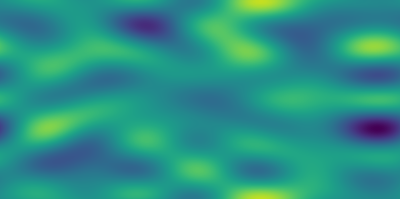
\includegraphics[interpolate=false,width=1.000000in,height=1.000000in]{burgers_rollout_target_0.0-img0.png}}%
\end{pgfscope}%
\begin{pgfscope}%
\pgfsetbuttcap%
\pgfsetroundjoin%
\definecolor{currentfill}{rgb}{0.000000,0.000000,0.000000}%
\pgfsetfillcolor{currentfill}%
\pgfsetlinewidth{0.803000pt}%
\definecolor{currentstroke}{rgb}{0.000000,0.000000,0.000000}%
\pgfsetstrokecolor{currentstroke}%
\pgfsetdash{}{0pt}%
\pgfsys@defobject{currentmarker}{\pgfqpoint{0.000000in}{-0.048611in}}{\pgfqpoint{0.000000in}{0.000000in}}{%
\pgfpathmoveto{\pgfqpoint{0.000000in}{0.000000in}}%
\pgfpathlineto{\pgfqpoint{0.000000in}{-0.048611in}}%
\pgfusepath{stroke,fill}%
}%
\begin{pgfscope}%
\pgfsys@transformshift{0.726837in}{0.517039in}%
\pgfsys@useobject{currentmarker}{}%
\end{pgfscope}%
\end{pgfscope}%
\begin{pgfscope}%
\definecolor{textcolor}{rgb}{0.000000,0.000000,0.000000}%
\pgfsetstrokecolor{textcolor}%
\pgfsetfillcolor{textcolor}%
\pgftext[x=0.726837in,y=0.419816in,,top]{\color{textcolor}{\rmfamily\fontsize{12.000000}{14.400000}\selectfont\catcode`\^=\active\def^{\ifmmode\sp\else\^{}\fi}\catcode`\%=\active\def%{\%}0}}%
\end{pgfscope}%
\begin{pgfscope}%
\pgfsetbuttcap%
\pgfsetroundjoin%
\definecolor{currentfill}{rgb}{0.000000,0.000000,0.000000}%
\pgfsetfillcolor{currentfill}%
\pgfsetlinewidth{0.803000pt}%
\definecolor{currentstroke}{rgb}{0.000000,0.000000,0.000000}%
\pgfsetstrokecolor{currentstroke}%
\pgfsetdash{}{0pt}%
\pgfsys@defobject{currentmarker}{\pgfqpoint{0.000000in}{-0.048611in}}{\pgfqpoint{0.000000in}{0.000000in}}{%
\pgfpathmoveto{\pgfqpoint{0.000000in}{0.000000in}}%
\pgfpathlineto{\pgfqpoint{0.000000in}{-0.048611in}}%
\pgfusepath{stroke,fill}%
}%
\begin{pgfscope}%
\pgfsys@transformshift{1.570762in}{0.517039in}%
\pgfsys@useobject{currentmarker}{}%
\end{pgfscope}%
\end{pgfscope}%
\begin{pgfscope}%
\definecolor{textcolor}{rgb}{0.000000,0.000000,0.000000}%
\pgfsetstrokecolor{textcolor}%
\pgfsetfillcolor{textcolor}%
\pgftext[x=1.570762in,y=0.419816in,,top]{\color{textcolor}{\rmfamily\fontsize{12.000000}{14.400000}\selectfont\catcode`\^=\active\def^{\ifmmode\sp\else\^{}\fi}\catcode`\%=\active\def%{\%}1}}%
\end{pgfscope}%
\begin{pgfscope}%
\pgfsetbuttcap%
\pgfsetroundjoin%
\definecolor{currentfill}{rgb}{0.000000,0.000000,0.000000}%
\pgfsetfillcolor{currentfill}%
\pgfsetlinewidth{0.803000pt}%
\definecolor{currentstroke}{rgb}{0.000000,0.000000,0.000000}%
\pgfsetstrokecolor{currentstroke}%
\pgfsetdash{}{0pt}%
\pgfsys@defobject{currentmarker}{\pgfqpoint{0.000000in}{-0.048611in}}{\pgfqpoint{0.000000in}{0.000000in}}{%
\pgfpathmoveto{\pgfqpoint{0.000000in}{0.000000in}}%
\pgfpathlineto{\pgfqpoint{0.000000in}{-0.048611in}}%
\pgfusepath{stroke,fill}%
}%
\begin{pgfscope}%
\pgfsys@transformshift{2.414687in}{0.517039in}%
\pgfsys@useobject{currentmarker}{}%
\end{pgfscope}%
\end{pgfscope}%
\begin{pgfscope}%
\definecolor{textcolor}{rgb}{0.000000,0.000000,0.000000}%
\pgfsetstrokecolor{textcolor}%
\pgfsetfillcolor{textcolor}%
\pgftext[x=2.414687in,y=0.419816in,,top]{\color{textcolor}{\rmfamily\fontsize{12.000000}{14.400000}\selectfont\catcode`\^=\active\def^{\ifmmode\sp\else\^{}\fi}\catcode`\%=\active\def%{\%}2}}%
\end{pgfscope}%
\begin{pgfscope}%
\definecolor{textcolor}{rgb}{0.000000,0.000000,0.000000}%
\pgfsetstrokecolor{textcolor}%
\pgfsetfillcolor{textcolor}%
\pgftext[x=1.570762in,y=0.202965in,,top]{\color{textcolor}{\rmfamily\fontsize{12.000000}{14.400000}\selectfont\catcode`\^=\active\def^{\ifmmode\sp\else\^{}\fi}\catcode`\%=\active\def%{\%}Space}}%
\end{pgfscope}%
\begin{pgfscope}%
\pgfsetbuttcap%
\pgfsetroundjoin%
\definecolor{currentfill}{rgb}{0.000000,0.000000,0.000000}%
\pgfsetfillcolor{currentfill}%
\pgfsetlinewidth{0.803000pt}%
\definecolor{currentstroke}{rgb}{0.000000,0.000000,0.000000}%
\pgfsetstrokecolor{currentstroke}%
\pgfsetdash{}{0pt}%
\pgfsys@defobject{currentmarker}{\pgfqpoint{-0.048611in}{0.000000in}}{\pgfqpoint{-0.000000in}{0.000000in}}{%
\pgfpathmoveto{\pgfqpoint{-0.000000in}{0.000000in}}%
\pgfpathlineto{\pgfqpoint{-0.048611in}{0.000000in}}%
\pgfusepath{stroke,fill}%
}%
\begin{pgfscope}%
\pgfsys@transformshift{0.726837in}{0.517039in}%
\pgfsys@useobject{currentmarker}{}%
\end{pgfscope}%
\end{pgfscope}%
\begin{pgfscope}%
\definecolor{textcolor}{rgb}{0.000000,0.000000,0.000000}%
\pgfsetstrokecolor{textcolor}%
\pgfsetfillcolor{textcolor}%
\pgftext[x=0.364559in, y=0.453725in, left, base]{\color{textcolor}{\rmfamily\fontsize{12.000000}{14.400000}\selectfont\catcode`\^=\active\def^{\ifmmode\sp\else\^{}\fi}\catcode`\%=\active\def%{\%}0.0}}%
\end{pgfscope}%
\begin{pgfscope}%
\pgfsetbuttcap%
\pgfsetroundjoin%
\definecolor{currentfill}{rgb}{0.000000,0.000000,0.000000}%
\pgfsetfillcolor{currentfill}%
\pgfsetlinewidth{0.803000pt}%
\definecolor{currentstroke}{rgb}{0.000000,0.000000,0.000000}%
\pgfsetstrokecolor{currentstroke}%
\pgfsetdash{}{0pt}%
\pgfsys@defobject{currentmarker}{\pgfqpoint{-0.048611in}{0.000000in}}{\pgfqpoint{-0.000000in}{0.000000in}}{%
\pgfpathmoveto{\pgfqpoint{-0.000000in}{0.000000in}}%
\pgfpathlineto{\pgfqpoint{-0.048611in}{0.000000in}}%
\pgfusepath{stroke,fill}%
}%
\begin{pgfscope}%
\pgfsys@transformshift{0.726837in}{0.861533in}%
\pgfsys@useobject{currentmarker}{}%
\end{pgfscope}%
\end{pgfscope}%
\begin{pgfscope}%
\definecolor{textcolor}{rgb}{0.000000,0.000000,0.000000}%
\pgfsetstrokecolor{textcolor}%
\pgfsetfillcolor{textcolor}%
\pgftext[x=0.364559in, y=0.798219in, left, base]{\color{textcolor}{\rmfamily\fontsize{12.000000}{14.400000}\selectfont\catcode`\^=\active\def^{\ifmmode\sp\else\^{}\fi}\catcode`\%=\active\def%{\%}2.5}}%
\end{pgfscope}%
\begin{pgfscope}%
\pgfsetbuttcap%
\pgfsetroundjoin%
\definecolor{currentfill}{rgb}{0.000000,0.000000,0.000000}%
\pgfsetfillcolor{currentfill}%
\pgfsetlinewidth{0.803000pt}%
\definecolor{currentstroke}{rgb}{0.000000,0.000000,0.000000}%
\pgfsetstrokecolor{currentstroke}%
\pgfsetdash{}{0pt}%
\pgfsys@defobject{currentmarker}{\pgfqpoint{-0.048611in}{0.000000in}}{\pgfqpoint{-0.000000in}{0.000000in}}{%
\pgfpathmoveto{\pgfqpoint{-0.000000in}{0.000000in}}%
\pgfpathlineto{\pgfqpoint{-0.048611in}{0.000000in}}%
\pgfusepath{stroke,fill}%
}%
\begin{pgfscope}%
\pgfsys@transformshift{0.726837in}{1.206027in}%
\pgfsys@useobject{currentmarker}{}%
\end{pgfscope}%
\end{pgfscope}%
\begin{pgfscope}%
\definecolor{textcolor}{rgb}{0.000000,0.000000,0.000000}%
\pgfsetstrokecolor{textcolor}%
\pgfsetfillcolor{textcolor}%
\pgftext[x=0.364559in, y=1.142714in, left, base]{\color{textcolor}{\rmfamily\fontsize{12.000000}{14.400000}\selectfont\catcode`\^=\active\def^{\ifmmode\sp\else\^{}\fi}\catcode`\%=\active\def%{\%}5.0}}%
\end{pgfscope}%
\begin{pgfscope}%
\pgfsetbuttcap%
\pgfsetroundjoin%
\definecolor{currentfill}{rgb}{0.000000,0.000000,0.000000}%
\pgfsetfillcolor{currentfill}%
\pgfsetlinewidth{0.803000pt}%
\definecolor{currentstroke}{rgb}{0.000000,0.000000,0.000000}%
\pgfsetstrokecolor{currentstroke}%
\pgfsetdash{}{0pt}%
\pgfsys@defobject{currentmarker}{\pgfqpoint{-0.048611in}{0.000000in}}{\pgfqpoint{-0.000000in}{0.000000in}}{%
\pgfpathmoveto{\pgfqpoint{-0.000000in}{0.000000in}}%
\pgfpathlineto{\pgfqpoint{-0.048611in}{0.000000in}}%
\pgfusepath{stroke,fill}%
}%
\begin{pgfscope}%
\pgfsys@transformshift{0.726837in}{1.550522in}%
\pgfsys@useobject{currentmarker}{}%
\end{pgfscope}%
\end{pgfscope}%
\begin{pgfscope}%
\definecolor{textcolor}{rgb}{0.000000,0.000000,0.000000}%
\pgfsetstrokecolor{textcolor}%
\pgfsetfillcolor{textcolor}%
\pgftext[x=0.364559in, y=1.487208in, left, base]{\color{textcolor}{\rmfamily\fontsize{12.000000}{14.400000}\selectfont\catcode`\^=\active\def^{\ifmmode\sp\else\^{}\fi}\catcode`\%=\active\def%{\%}7.5}}%
\end{pgfscope}%
\begin{pgfscope}%
\pgfsetbuttcap%
\pgfsetroundjoin%
\definecolor{currentfill}{rgb}{0.000000,0.000000,0.000000}%
\pgfsetfillcolor{currentfill}%
\pgfsetlinewidth{0.803000pt}%
\definecolor{currentstroke}{rgb}{0.000000,0.000000,0.000000}%
\pgfsetstrokecolor{currentstroke}%
\pgfsetdash{}{0pt}%
\pgfsys@defobject{currentmarker}{\pgfqpoint{-0.048611in}{0.000000in}}{\pgfqpoint{-0.000000in}{0.000000in}}{%
\pgfpathmoveto{\pgfqpoint{-0.000000in}{0.000000in}}%
\pgfpathlineto{\pgfqpoint{-0.048611in}{0.000000in}}%
\pgfusepath{stroke,fill}%
}%
\begin{pgfscope}%
\pgfsys@transformshift{0.726837in}{1.895016in}%
\pgfsys@useobject{currentmarker}{}%
\end{pgfscope}%
\end{pgfscope}%
\begin{pgfscope}%
\definecolor{textcolor}{rgb}{0.000000,0.000000,0.000000}%
\pgfsetstrokecolor{textcolor}%
\pgfsetfillcolor{textcolor}%
\pgftext[x=0.258521in, y=1.831702in, left, base]{\color{textcolor}{\rmfamily\fontsize{12.000000}{14.400000}\selectfont\catcode`\^=\active\def^{\ifmmode\sp\else\^{}\fi}\catcode`\%=\active\def%{\%}10.0}}%
\end{pgfscope}%
\begin{pgfscope}%
\definecolor{textcolor}{rgb}{0.000000,0.000000,0.000000}%
\pgfsetstrokecolor{textcolor}%
\pgfsetfillcolor{textcolor}%
\pgftext[x=0.202965in,y=1.206027in,,bottom,rotate=90.000000]{\color{textcolor}{\rmfamily\fontsize{12.000000}{14.400000}\selectfont\catcode`\^=\active\def^{\ifmmode\sp\else\^{}\fi}\catcode`\%=\active\def%{\%}Time}}%
\end{pgfscope}%
\begin{pgfscope}%
\pgfsetrectcap%
\pgfsetmiterjoin%
\pgfsetlinewidth{0.803000pt}%
\definecolor{currentstroke}{rgb}{0.000000,0.000000,0.000000}%
\pgfsetstrokecolor{currentstroke}%
\pgfsetdash{}{0pt}%
\pgfpathmoveto{\pgfqpoint{0.726837in}{0.517039in}}%
\pgfpathlineto{\pgfqpoint{0.726837in}{1.895016in}}%
\pgfusepath{stroke}%
\end{pgfscope}%
\begin{pgfscope}%
\pgfsetrectcap%
\pgfsetmiterjoin%
\pgfsetlinewidth{0.803000pt}%
\definecolor{currentstroke}{rgb}{0.000000,0.000000,0.000000}%
\pgfsetstrokecolor{currentstroke}%
\pgfsetdash{}{0pt}%
\pgfpathmoveto{\pgfqpoint{2.414687in}{0.517039in}}%
\pgfpathlineto{\pgfqpoint{2.414687in}{1.895016in}}%
\pgfusepath{stroke}%
\end{pgfscope}%
\begin{pgfscope}%
\pgfsetrectcap%
\pgfsetmiterjoin%
\pgfsetlinewidth{0.803000pt}%
\definecolor{currentstroke}{rgb}{0.000000,0.000000,0.000000}%
\pgfsetstrokecolor{currentstroke}%
\pgfsetdash{}{0pt}%
\pgfpathmoveto{\pgfqpoint{0.726837in}{0.517039in}}%
\pgfpathlineto{\pgfqpoint{2.414687in}{0.517039in}}%
\pgfusepath{stroke}%
\end{pgfscope}%
\begin{pgfscope}%
\pgfsetrectcap%
\pgfsetmiterjoin%
\pgfsetlinewidth{0.803000pt}%
\definecolor{currentstroke}{rgb}{0.000000,0.000000,0.000000}%
\pgfsetstrokecolor{currentstroke}%
\pgfsetdash{}{0pt}%
\pgfpathmoveto{\pgfqpoint{0.726837in}{1.895016in}}%
\pgfpathlineto{\pgfqpoint{2.414687in}{1.895016in}}%
\pgfusepath{stroke}%
\end{pgfscope}%
\begin{pgfscope}%
\pgfsetbuttcap%
\pgfsetmiterjoin%
\pgfsetlinewidth{0.000000pt}%
\definecolor{currentstroke}{rgb}{0.000000,0.000000,0.000000}%
\pgfsetstrokecolor{currentstroke}%
\pgfsetstrokeopacity{0.000000}%
\pgfsetdash{}{0pt}%
\pgfpathmoveto{\pgfqpoint{2.552099in}{0.517039in}}%
\pgfpathlineto{\pgfqpoint{2.620998in}{0.517039in}}%
\pgfpathlineto{\pgfqpoint{2.620998in}{1.895016in}}%
\pgfpathlineto{\pgfqpoint{2.552099in}{1.895016in}}%
\pgfpathlineto{\pgfqpoint{2.552099in}{0.517039in}}%
\pgfpathclose%
\pgfusepath{}%
\end{pgfscope}%
\begin{pgfscope}%
\pgfsys@transformshift{2.550000in}{0.520000in}%
\pgftext[left,bottom]{
\includegraphics[interpolate=true,width=0.070000in,height=1.380000in]{burgers_rollout_target_0.0-img1.png}}%
\end{pgfscope}%
\begin{pgfscope}%
\pgfsetbuttcap%
\pgfsetroundjoin%
\definecolor{currentfill}{rgb}{0.000000,0.000000,0.000000}%
\pgfsetfillcolor{currentfill}%
\pgfsetlinewidth{0.803000pt}%
\definecolor{currentstroke}{rgb}{0.000000,0.000000,0.000000}%
\pgfsetstrokecolor{currentstroke}%
\pgfsetdash{}{0pt}%
\pgfsys@defobject{currentmarker}{\pgfqpoint{0.000000in}{0.000000in}}{\pgfqpoint{0.048611in}{0.000000in}}{%
\pgfpathmoveto{\pgfqpoint{0.000000in}{0.000000in}}%
\pgfpathlineto{\pgfqpoint{0.048611in}{0.000000in}}%
\pgfusepath{stroke,fill}%
}%
\begin{pgfscope}%
\pgfsys@transformshift{2.620998in}{0.588723in}%
\pgfsys@useobject{currentmarker}{}%
\end{pgfscope}%
\end{pgfscope}%
\begin{pgfscope}%
\definecolor{textcolor}{rgb}{0.000000,0.000000,0.000000}%
\pgfsetstrokecolor{textcolor}%
\pgfsetfillcolor{textcolor}%
\pgftext[x=2.718220in, y=0.525410in, left, base]{\color{textcolor}{\rmfamily\fontsize{12.000000}{14.400000}\selectfont\catcode`\^=\active\def^{\ifmmode\sp\else\^{}\fi}\catcode`\%=\active\def%{\%}\ensuremath{-}1}}%
\end{pgfscope}%
\begin{pgfscope}%
\pgfsetbuttcap%
\pgfsetroundjoin%
\definecolor{currentfill}{rgb}{0.000000,0.000000,0.000000}%
\pgfsetfillcolor{currentfill}%
\pgfsetlinewidth{0.803000pt}%
\definecolor{currentstroke}{rgb}{0.000000,0.000000,0.000000}%
\pgfsetstrokecolor{currentstroke}%
\pgfsetdash{}{0pt}%
\pgfsys@defobject{currentmarker}{\pgfqpoint{0.000000in}{0.000000in}}{\pgfqpoint{0.048611in}{0.000000in}}{%
\pgfpathmoveto{\pgfqpoint{0.000000in}{0.000000in}}%
\pgfpathlineto{\pgfqpoint{0.048611in}{0.000000in}}%
\pgfusepath{stroke,fill}%
}%
\begin{pgfscope}%
\pgfsys@transformshift{2.620998in}{1.206027in}%
\pgfsys@useobject{currentmarker}{}%
\end{pgfscope}%
\end{pgfscope}%
\begin{pgfscope}%
\definecolor{textcolor}{rgb}{0.000000,0.000000,0.000000}%
\pgfsetstrokecolor{textcolor}%
\pgfsetfillcolor{textcolor}%
\pgftext[x=2.718220in, y=1.142714in, left, base]{\color{textcolor}{\rmfamily\fontsize{12.000000}{14.400000}\selectfont\catcode`\^=\active\def^{\ifmmode\sp\else\^{}\fi}\catcode`\%=\active\def%{\%}0}}%
\end{pgfscope}%
\begin{pgfscope}%
\pgfsetbuttcap%
\pgfsetroundjoin%
\definecolor{currentfill}{rgb}{0.000000,0.000000,0.000000}%
\pgfsetfillcolor{currentfill}%
\pgfsetlinewidth{0.803000pt}%
\definecolor{currentstroke}{rgb}{0.000000,0.000000,0.000000}%
\pgfsetstrokecolor{currentstroke}%
\pgfsetdash{}{0pt}%
\pgfsys@defobject{currentmarker}{\pgfqpoint{0.000000in}{0.000000in}}{\pgfqpoint{0.048611in}{0.000000in}}{%
\pgfpathmoveto{\pgfqpoint{0.000000in}{0.000000in}}%
\pgfpathlineto{\pgfqpoint{0.048611in}{0.000000in}}%
\pgfusepath{stroke,fill}%
}%
\begin{pgfscope}%
\pgfsys@transformshift{2.620998in}{1.823331in}%
\pgfsys@useobject{currentmarker}{}%
\end{pgfscope}%
\end{pgfscope}%
\begin{pgfscope}%
\definecolor{textcolor}{rgb}{0.000000,0.000000,0.000000}%
\pgfsetstrokecolor{textcolor}%
\pgfsetfillcolor{textcolor}%
\pgftext[x=2.718220in, y=1.760018in, left, base]{\color{textcolor}{\rmfamily\fontsize{12.000000}{14.400000}\selectfont\catcode`\^=\active\def^{\ifmmode\sp\else\^{}\fi}\catcode`\%=\active\def%{\%}1}}%
\end{pgfscope}%
\begin{pgfscope}%
\pgfsetrectcap%
\pgfsetmiterjoin%
\pgfsetlinewidth{0.803000pt}%
\definecolor{currentstroke}{rgb}{0.000000,0.000000,0.000000}%
\pgfsetstrokecolor{currentstroke}%
\pgfsetdash{}{0pt}%
\pgfpathmoveto{\pgfqpoint{2.552099in}{0.517039in}}%
\pgfpathlineto{\pgfqpoint{2.586548in}{0.517039in}}%
\pgfpathlineto{\pgfqpoint{2.620998in}{0.517039in}}%
\pgfpathlineto{\pgfqpoint{2.620998in}{1.895016in}}%
\pgfpathlineto{\pgfqpoint{2.586548in}{1.895016in}}%
\pgfpathlineto{\pgfqpoint{2.552099in}{1.895016in}}%
\pgfpathlineto{\pgfqpoint{2.552099in}{0.517039in}}%
\pgfpathclose%
\pgfusepath{stroke}%
\end{pgfscope}%
\end{pgfpicture}%
\makeatother%
\endgroup%

      \end{adjustbox}
      \caption{The target for \(\nu=0.0\)}\label{fig:sc2_rollout_target_0.0}
    \end{subfigure}
    \begin{subfigure}{0.33\linewidth}
      \begin{adjustbox}{width=\linewidth}
        \begingroup%
\makeatletter%
\begin{pgfpicture}%
\pgfpathrectangle{\pgfpointorigin}{\pgfqpoint{3.000000in}{2.000000in}}%
\pgfusepath{use as bounding box, clip}%
\begin{pgfscope}%
\pgfsetbuttcap%
\pgfsetmiterjoin%
\pgfsetlinewidth{0.000000pt}%
\definecolor{currentstroke}{rgb}{0.000000,0.000000,0.000000}%
\pgfsetstrokecolor{currentstroke}%
\pgfsetstrokeopacity{0.000000}%
\pgfsetdash{}{0pt}%
\pgfpathmoveto{\pgfqpoint{0.000000in}{0.000000in}}%
\pgfpathlineto{\pgfqpoint{3.000000in}{0.000000in}}%
\pgfpathlineto{\pgfqpoint{3.000000in}{2.000000in}}%
\pgfpathlineto{\pgfqpoint{0.000000in}{2.000000in}}%
\pgfpathlineto{\pgfqpoint{0.000000in}{0.000000in}}%
\pgfpathclose%
\pgfusepath{}%
\end{pgfscope}%
\begin{pgfscope}%
\pgfsetbuttcap%
\pgfsetmiterjoin%
\pgfsetlinewidth{0.000000pt}%
\definecolor{currentstroke}{rgb}{0.000000,0.000000,0.000000}%
\pgfsetstrokecolor{currentstroke}%
\pgfsetstrokeopacity{0.000000}%
\pgfsetdash{}{0pt}%
\pgfpathmoveto{\pgfqpoint{0.726837in}{0.517039in}}%
\pgfpathlineto{\pgfqpoint{2.414687in}{0.517039in}}%
\pgfpathlineto{\pgfqpoint{2.414687in}{1.895016in}}%
\pgfpathlineto{\pgfqpoint{0.726837in}{1.895016in}}%
\pgfpathlineto{\pgfqpoint{0.726837in}{0.517039in}}%
\pgfpathclose%
\pgfusepath{}%
\end{pgfscope}%
\begin{pgfscope}%
\pgfpathrectangle{\pgfqpoint{0.726837in}{0.517039in}}{\pgfqpoint{1.687850in}{1.377978in}}%
\pgfusepath{clip}%
\pgfsys@transformcm{1.687850}{0.000000}{0.000000}{1.377978}{0.726837in}{0.517039in}%
\pgftext[left,bottom]{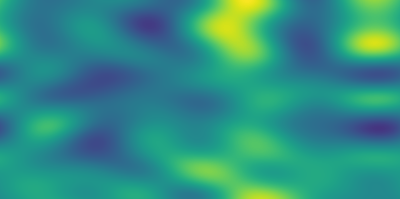
\includegraphics[interpolate=false,width=1.000000in,height=1.000000in]{burgers_rollout_pred_0.0-img0.png}}%
\end{pgfscope}%
\begin{pgfscope}%
\pgfsetbuttcap%
\pgfsetroundjoin%
\definecolor{currentfill}{rgb}{0.000000,0.000000,0.000000}%
\pgfsetfillcolor{currentfill}%
\pgfsetlinewidth{0.803000pt}%
\definecolor{currentstroke}{rgb}{0.000000,0.000000,0.000000}%
\pgfsetstrokecolor{currentstroke}%
\pgfsetdash{}{0pt}%
\pgfsys@defobject{currentmarker}{\pgfqpoint{0.000000in}{-0.048611in}}{\pgfqpoint{0.000000in}{0.000000in}}{%
\pgfpathmoveto{\pgfqpoint{0.000000in}{0.000000in}}%
\pgfpathlineto{\pgfqpoint{0.000000in}{-0.048611in}}%
\pgfusepath{stroke,fill}%
}%
\begin{pgfscope}%
\pgfsys@transformshift{0.726837in}{0.517039in}%
\pgfsys@useobject{currentmarker}{}%
\end{pgfscope}%
\end{pgfscope}%
\begin{pgfscope}%
\definecolor{textcolor}{rgb}{0.000000,0.000000,0.000000}%
\pgfsetstrokecolor{textcolor}%
\pgfsetfillcolor{textcolor}%
\pgftext[x=0.726837in,y=0.419816in,,top]{\color{textcolor}{\rmfamily\fontsize{12.000000}{14.400000}\selectfont\catcode`\^=\active\def^{\ifmmode\sp\else\^{}\fi}\catcode`\%=\active\def%{\%}0}}%
\end{pgfscope}%
\begin{pgfscope}%
\pgfsetbuttcap%
\pgfsetroundjoin%
\definecolor{currentfill}{rgb}{0.000000,0.000000,0.000000}%
\pgfsetfillcolor{currentfill}%
\pgfsetlinewidth{0.803000pt}%
\definecolor{currentstroke}{rgb}{0.000000,0.000000,0.000000}%
\pgfsetstrokecolor{currentstroke}%
\pgfsetdash{}{0pt}%
\pgfsys@defobject{currentmarker}{\pgfqpoint{0.000000in}{-0.048611in}}{\pgfqpoint{0.000000in}{0.000000in}}{%
\pgfpathmoveto{\pgfqpoint{0.000000in}{0.000000in}}%
\pgfpathlineto{\pgfqpoint{0.000000in}{-0.048611in}}%
\pgfusepath{stroke,fill}%
}%
\begin{pgfscope}%
\pgfsys@transformshift{1.570762in}{0.517039in}%
\pgfsys@useobject{currentmarker}{}%
\end{pgfscope}%
\end{pgfscope}%
\begin{pgfscope}%
\definecolor{textcolor}{rgb}{0.000000,0.000000,0.000000}%
\pgfsetstrokecolor{textcolor}%
\pgfsetfillcolor{textcolor}%
\pgftext[x=1.570762in,y=0.419816in,,top]{\color{textcolor}{\rmfamily\fontsize{12.000000}{14.400000}\selectfont\catcode`\^=\active\def^{\ifmmode\sp\else\^{}\fi}\catcode`\%=\active\def%{\%}1}}%
\end{pgfscope}%
\begin{pgfscope}%
\pgfsetbuttcap%
\pgfsetroundjoin%
\definecolor{currentfill}{rgb}{0.000000,0.000000,0.000000}%
\pgfsetfillcolor{currentfill}%
\pgfsetlinewidth{0.803000pt}%
\definecolor{currentstroke}{rgb}{0.000000,0.000000,0.000000}%
\pgfsetstrokecolor{currentstroke}%
\pgfsetdash{}{0pt}%
\pgfsys@defobject{currentmarker}{\pgfqpoint{0.000000in}{-0.048611in}}{\pgfqpoint{0.000000in}{0.000000in}}{%
\pgfpathmoveto{\pgfqpoint{0.000000in}{0.000000in}}%
\pgfpathlineto{\pgfqpoint{0.000000in}{-0.048611in}}%
\pgfusepath{stroke,fill}%
}%
\begin{pgfscope}%
\pgfsys@transformshift{2.414687in}{0.517039in}%
\pgfsys@useobject{currentmarker}{}%
\end{pgfscope}%
\end{pgfscope}%
\begin{pgfscope}%
\definecolor{textcolor}{rgb}{0.000000,0.000000,0.000000}%
\pgfsetstrokecolor{textcolor}%
\pgfsetfillcolor{textcolor}%
\pgftext[x=2.414687in,y=0.419816in,,top]{\color{textcolor}{\rmfamily\fontsize{12.000000}{14.400000}\selectfont\catcode`\^=\active\def^{\ifmmode\sp\else\^{}\fi}\catcode`\%=\active\def%{\%}2}}%
\end{pgfscope}%
\begin{pgfscope}%
\definecolor{textcolor}{rgb}{0.000000,0.000000,0.000000}%
\pgfsetstrokecolor{textcolor}%
\pgfsetfillcolor{textcolor}%
\pgftext[x=1.570762in,y=0.202965in,,top]{\color{textcolor}{\rmfamily\fontsize{12.000000}{14.400000}\selectfont\catcode`\^=\active\def^{\ifmmode\sp\else\^{}\fi}\catcode`\%=\active\def%{\%}Space}}%
\end{pgfscope}%
\begin{pgfscope}%
\pgfsetbuttcap%
\pgfsetroundjoin%
\definecolor{currentfill}{rgb}{0.000000,0.000000,0.000000}%
\pgfsetfillcolor{currentfill}%
\pgfsetlinewidth{0.803000pt}%
\definecolor{currentstroke}{rgb}{0.000000,0.000000,0.000000}%
\pgfsetstrokecolor{currentstroke}%
\pgfsetdash{}{0pt}%
\pgfsys@defobject{currentmarker}{\pgfqpoint{-0.048611in}{0.000000in}}{\pgfqpoint{-0.000000in}{0.000000in}}{%
\pgfpathmoveto{\pgfqpoint{-0.000000in}{0.000000in}}%
\pgfpathlineto{\pgfqpoint{-0.048611in}{0.000000in}}%
\pgfusepath{stroke,fill}%
}%
\begin{pgfscope}%
\pgfsys@transformshift{0.726837in}{0.517039in}%
\pgfsys@useobject{currentmarker}{}%
\end{pgfscope}%
\end{pgfscope}%
\begin{pgfscope}%
\definecolor{textcolor}{rgb}{0.000000,0.000000,0.000000}%
\pgfsetstrokecolor{textcolor}%
\pgfsetfillcolor{textcolor}%
\pgftext[x=0.364559in, y=0.453725in, left, base]{\color{textcolor}{\rmfamily\fontsize{12.000000}{14.400000}\selectfont\catcode`\^=\active\def^{\ifmmode\sp\else\^{}\fi}\catcode`\%=\active\def%{\%}0.0}}%
\end{pgfscope}%
\begin{pgfscope}%
\pgfsetbuttcap%
\pgfsetroundjoin%
\definecolor{currentfill}{rgb}{0.000000,0.000000,0.000000}%
\pgfsetfillcolor{currentfill}%
\pgfsetlinewidth{0.803000pt}%
\definecolor{currentstroke}{rgb}{0.000000,0.000000,0.000000}%
\pgfsetstrokecolor{currentstroke}%
\pgfsetdash{}{0pt}%
\pgfsys@defobject{currentmarker}{\pgfqpoint{-0.048611in}{0.000000in}}{\pgfqpoint{-0.000000in}{0.000000in}}{%
\pgfpathmoveto{\pgfqpoint{-0.000000in}{0.000000in}}%
\pgfpathlineto{\pgfqpoint{-0.048611in}{0.000000in}}%
\pgfusepath{stroke,fill}%
}%
\begin{pgfscope}%
\pgfsys@transformshift{0.726837in}{0.861533in}%
\pgfsys@useobject{currentmarker}{}%
\end{pgfscope}%
\end{pgfscope}%
\begin{pgfscope}%
\definecolor{textcolor}{rgb}{0.000000,0.000000,0.000000}%
\pgfsetstrokecolor{textcolor}%
\pgfsetfillcolor{textcolor}%
\pgftext[x=0.364559in, y=0.798219in, left, base]{\color{textcolor}{\rmfamily\fontsize{12.000000}{14.400000}\selectfont\catcode`\^=\active\def^{\ifmmode\sp\else\^{}\fi}\catcode`\%=\active\def%{\%}2.5}}%
\end{pgfscope}%
\begin{pgfscope}%
\pgfsetbuttcap%
\pgfsetroundjoin%
\definecolor{currentfill}{rgb}{0.000000,0.000000,0.000000}%
\pgfsetfillcolor{currentfill}%
\pgfsetlinewidth{0.803000pt}%
\definecolor{currentstroke}{rgb}{0.000000,0.000000,0.000000}%
\pgfsetstrokecolor{currentstroke}%
\pgfsetdash{}{0pt}%
\pgfsys@defobject{currentmarker}{\pgfqpoint{-0.048611in}{0.000000in}}{\pgfqpoint{-0.000000in}{0.000000in}}{%
\pgfpathmoveto{\pgfqpoint{-0.000000in}{0.000000in}}%
\pgfpathlineto{\pgfqpoint{-0.048611in}{0.000000in}}%
\pgfusepath{stroke,fill}%
}%
\begin{pgfscope}%
\pgfsys@transformshift{0.726837in}{1.206027in}%
\pgfsys@useobject{currentmarker}{}%
\end{pgfscope}%
\end{pgfscope}%
\begin{pgfscope}%
\definecolor{textcolor}{rgb}{0.000000,0.000000,0.000000}%
\pgfsetstrokecolor{textcolor}%
\pgfsetfillcolor{textcolor}%
\pgftext[x=0.364559in, y=1.142714in, left, base]{\color{textcolor}{\rmfamily\fontsize{12.000000}{14.400000}\selectfont\catcode`\^=\active\def^{\ifmmode\sp\else\^{}\fi}\catcode`\%=\active\def%{\%}5.0}}%
\end{pgfscope}%
\begin{pgfscope}%
\pgfsetbuttcap%
\pgfsetroundjoin%
\definecolor{currentfill}{rgb}{0.000000,0.000000,0.000000}%
\pgfsetfillcolor{currentfill}%
\pgfsetlinewidth{0.803000pt}%
\definecolor{currentstroke}{rgb}{0.000000,0.000000,0.000000}%
\pgfsetstrokecolor{currentstroke}%
\pgfsetdash{}{0pt}%
\pgfsys@defobject{currentmarker}{\pgfqpoint{-0.048611in}{0.000000in}}{\pgfqpoint{-0.000000in}{0.000000in}}{%
\pgfpathmoveto{\pgfqpoint{-0.000000in}{0.000000in}}%
\pgfpathlineto{\pgfqpoint{-0.048611in}{0.000000in}}%
\pgfusepath{stroke,fill}%
}%
\begin{pgfscope}%
\pgfsys@transformshift{0.726837in}{1.550522in}%
\pgfsys@useobject{currentmarker}{}%
\end{pgfscope}%
\end{pgfscope}%
\begin{pgfscope}%
\definecolor{textcolor}{rgb}{0.000000,0.000000,0.000000}%
\pgfsetstrokecolor{textcolor}%
\pgfsetfillcolor{textcolor}%
\pgftext[x=0.364559in, y=1.487208in, left, base]{\color{textcolor}{\rmfamily\fontsize{12.000000}{14.400000}\selectfont\catcode`\^=\active\def^{\ifmmode\sp\else\^{}\fi}\catcode`\%=\active\def%{\%}7.5}}%
\end{pgfscope}%
\begin{pgfscope}%
\pgfsetbuttcap%
\pgfsetroundjoin%
\definecolor{currentfill}{rgb}{0.000000,0.000000,0.000000}%
\pgfsetfillcolor{currentfill}%
\pgfsetlinewidth{0.803000pt}%
\definecolor{currentstroke}{rgb}{0.000000,0.000000,0.000000}%
\pgfsetstrokecolor{currentstroke}%
\pgfsetdash{}{0pt}%
\pgfsys@defobject{currentmarker}{\pgfqpoint{-0.048611in}{0.000000in}}{\pgfqpoint{-0.000000in}{0.000000in}}{%
\pgfpathmoveto{\pgfqpoint{-0.000000in}{0.000000in}}%
\pgfpathlineto{\pgfqpoint{-0.048611in}{0.000000in}}%
\pgfusepath{stroke,fill}%
}%
\begin{pgfscope}%
\pgfsys@transformshift{0.726837in}{1.895016in}%
\pgfsys@useobject{currentmarker}{}%
\end{pgfscope}%
\end{pgfscope}%
\begin{pgfscope}%
\definecolor{textcolor}{rgb}{0.000000,0.000000,0.000000}%
\pgfsetstrokecolor{textcolor}%
\pgfsetfillcolor{textcolor}%
\pgftext[x=0.258521in, y=1.831702in, left, base]{\color{textcolor}{\rmfamily\fontsize{12.000000}{14.400000}\selectfont\catcode`\^=\active\def^{\ifmmode\sp\else\^{}\fi}\catcode`\%=\active\def%{\%}10.0}}%
\end{pgfscope}%
\begin{pgfscope}%
\definecolor{textcolor}{rgb}{0.000000,0.000000,0.000000}%
\pgfsetstrokecolor{textcolor}%
\pgfsetfillcolor{textcolor}%
\pgftext[x=0.202965in,y=1.206027in,,bottom,rotate=90.000000]{\color{textcolor}{\rmfamily\fontsize{12.000000}{14.400000}\selectfont\catcode`\^=\active\def^{\ifmmode\sp\else\^{}\fi}\catcode`\%=\active\def%{\%}Time}}%
\end{pgfscope}%
\begin{pgfscope}%
\pgfsetrectcap%
\pgfsetmiterjoin%
\pgfsetlinewidth{0.803000pt}%
\definecolor{currentstroke}{rgb}{0.000000,0.000000,0.000000}%
\pgfsetstrokecolor{currentstroke}%
\pgfsetdash{}{0pt}%
\pgfpathmoveto{\pgfqpoint{0.726837in}{0.517039in}}%
\pgfpathlineto{\pgfqpoint{0.726837in}{1.895016in}}%
\pgfusepath{stroke}%
\end{pgfscope}%
\begin{pgfscope}%
\pgfsetrectcap%
\pgfsetmiterjoin%
\pgfsetlinewidth{0.803000pt}%
\definecolor{currentstroke}{rgb}{0.000000,0.000000,0.000000}%
\pgfsetstrokecolor{currentstroke}%
\pgfsetdash{}{0pt}%
\pgfpathmoveto{\pgfqpoint{2.414687in}{0.517039in}}%
\pgfpathlineto{\pgfqpoint{2.414687in}{1.895016in}}%
\pgfusepath{stroke}%
\end{pgfscope}%
\begin{pgfscope}%
\pgfsetrectcap%
\pgfsetmiterjoin%
\pgfsetlinewidth{0.803000pt}%
\definecolor{currentstroke}{rgb}{0.000000,0.000000,0.000000}%
\pgfsetstrokecolor{currentstroke}%
\pgfsetdash{}{0pt}%
\pgfpathmoveto{\pgfqpoint{0.726837in}{0.517039in}}%
\pgfpathlineto{\pgfqpoint{2.414687in}{0.517039in}}%
\pgfusepath{stroke}%
\end{pgfscope}%
\begin{pgfscope}%
\pgfsetrectcap%
\pgfsetmiterjoin%
\pgfsetlinewidth{0.803000pt}%
\definecolor{currentstroke}{rgb}{0.000000,0.000000,0.000000}%
\pgfsetstrokecolor{currentstroke}%
\pgfsetdash{}{0pt}%
\pgfpathmoveto{\pgfqpoint{0.726837in}{1.895016in}}%
\pgfpathlineto{\pgfqpoint{2.414687in}{1.895016in}}%
\pgfusepath{stroke}%
\end{pgfscope}%
\begin{pgfscope}%
\pgfsetbuttcap%
\pgfsetmiterjoin%
\pgfsetlinewidth{0.000000pt}%
\definecolor{currentstroke}{rgb}{0.000000,0.000000,0.000000}%
\pgfsetstrokecolor{currentstroke}%
\pgfsetstrokeopacity{0.000000}%
\pgfsetdash{}{0pt}%
\pgfpathmoveto{\pgfqpoint{2.552099in}{0.517039in}}%
\pgfpathlineto{\pgfqpoint{2.620998in}{0.517039in}}%
\pgfpathlineto{\pgfqpoint{2.620998in}{1.895016in}}%
\pgfpathlineto{\pgfqpoint{2.552099in}{1.895016in}}%
\pgfpathlineto{\pgfqpoint{2.552099in}{0.517039in}}%
\pgfpathclose%
\pgfusepath{}%
\end{pgfscope}%
\begin{pgfscope}%
\pgfsys@transformshift{2.550000in}{0.520000in}%
\pgftext[left,bottom]{
\includegraphics[interpolate=true,width=0.070000in,height=1.380000in]{burgers_rollout_pred_0.0-img1.png}}%
\end{pgfscope}%
\begin{pgfscope}%
\pgfsetbuttcap%
\pgfsetroundjoin%
\definecolor{currentfill}{rgb}{0.000000,0.000000,0.000000}%
\pgfsetfillcolor{currentfill}%
\pgfsetlinewidth{0.803000pt}%
\definecolor{currentstroke}{rgb}{0.000000,0.000000,0.000000}%
\pgfsetstrokecolor{currentstroke}%
\pgfsetdash{}{0pt}%
\pgfsys@defobject{currentmarker}{\pgfqpoint{0.000000in}{0.000000in}}{\pgfqpoint{0.048611in}{0.000000in}}{%
\pgfpathmoveto{\pgfqpoint{0.000000in}{0.000000in}}%
\pgfpathlineto{\pgfqpoint{0.048611in}{0.000000in}}%
\pgfusepath{stroke,fill}%
}%
\begin{pgfscope}%
\pgfsys@transformshift{2.620998in}{0.588723in}%
\pgfsys@useobject{currentmarker}{}%
\end{pgfscope}%
\end{pgfscope}%
\begin{pgfscope}%
\definecolor{textcolor}{rgb}{0.000000,0.000000,0.000000}%
\pgfsetstrokecolor{textcolor}%
\pgfsetfillcolor{textcolor}%
\pgftext[x=2.718220in, y=0.525410in, left, base]{\color{textcolor}{\rmfamily\fontsize{12.000000}{14.400000}\selectfont\catcode`\^=\active\def^{\ifmmode\sp\else\^{}\fi}\catcode`\%=\active\def%{\%}\ensuremath{-}1}}%
\end{pgfscope}%
\begin{pgfscope}%
\pgfsetbuttcap%
\pgfsetroundjoin%
\definecolor{currentfill}{rgb}{0.000000,0.000000,0.000000}%
\pgfsetfillcolor{currentfill}%
\pgfsetlinewidth{0.803000pt}%
\definecolor{currentstroke}{rgb}{0.000000,0.000000,0.000000}%
\pgfsetstrokecolor{currentstroke}%
\pgfsetdash{}{0pt}%
\pgfsys@defobject{currentmarker}{\pgfqpoint{0.000000in}{0.000000in}}{\pgfqpoint{0.048611in}{0.000000in}}{%
\pgfpathmoveto{\pgfqpoint{0.000000in}{0.000000in}}%
\pgfpathlineto{\pgfqpoint{0.048611in}{0.000000in}}%
\pgfusepath{stroke,fill}%
}%
\begin{pgfscope}%
\pgfsys@transformshift{2.620998in}{1.206027in}%
\pgfsys@useobject{currentmarker}{}%
\end{pgfscope}%
\end{pgfscope}%
\begin{pgfscope}%
\definecolor{textcolor}{rgb}{0.000000,0.000000,0.000000}%
\pgfsetstrokecolor{textcolor}%
\pgfsetfillcolor{textcolor}%
\pgftext[x=2.718220in, y=1.142714in, left, base]{\color{textcolor}{\rmfamily\fontsize{12.000000}{14.400000}\selectfont\catcode`\^=\active\def^{\ifmmode\sp\else\^{}\fi}\catcode`\%=\active\def%{\%}0}}%
\end{pgfscope}%
\begin{pgfscope}%
\pgfsetbuttcap%
\pgfsetroundjoin%
\definecolor{currentfill}{rgb}{0.000000,0.000000,0.000000}%
\pgfsetfillcolor{currentfill}%
\pgfsetlinewidth{0.803000pt}%
\definecolor{currentstroke}{rgb}{0.000000,0.000000,0.000000}%
\pgfsetstrokecolor{currentstroke}%
\pgfsetdash{}{0pt}%
\pgfsys@defobject{currentmarker}{\pgfqpoint{0.000000in}{0.000000in}}{\pgfqpoint{0.048611in}{0.000000in}}{%
\pgfpathmoveto{\pgfqpoint{0.000000in}{0.000000in}}%
\pgfpathlineto{\pgfqpoint{0.048611in}{0.000000in}}%
\pgfusepath{stroke,fill}%
}%
\begin{pgfscope}%
\pgfsys@transformshift{2.620998in}{1.823331in}%
\pgfsys@useobject{currentmarker}{}%
\end{pgfscope}%
\end{pgfscope}%
\begin{pgfscope}%
\definecolor{textcolor}{rgb}{0.000000,0.000000,0.000000}%
\pgfsetstrokecolor{textcolor}%
\pgfsetfillcolor{textcolor}%
\pgftext[x=2.718220in, y=1.760018in, left, base]{\color{textcolor}{\rmfamily\fontsize{12.000000}{14.400000}\selectfont\catcode`\^=\active\def^{\ifmmode\sp\else\^{}\fi}\catcode`\%=\active\def%{\%}1}}%
\end{pgfscope}%
\begin{pgfscope}%
\pgfsetrectcap%
\pgfsetmiterjoin%
\pgfsetlinewidth{0.803000pt}%
\definecolor{currentstroke}{rgb}{0.000000,0.000000,0.000000}%
\pgfsetstrokecolor{currentstroke}%
\pgfsetdash{}{0pt}%
\pgfpathmoveto{\pgfqpoint{2.552099in}{0.517039in}}%
\pgfpathlineto{\pgfqpoint{2.586548in}{0.517039in}}%
\pgfpathlineto{\pgfqpoint{2.620998in}{0.517039in}}%
\pgfpathlineto{\pgfqpoint{2.620998in}{1.895016in}}%
\pgfpathlineto{\pgfqpoint{2.586548in}{1.895016in}}%
\pgfpathlineto{\pgfqpoint{2.552099in}{1.895016in}}%
\pgfpathlineto{\pgfqpoint{2.552099in}{0.517039in}}%
\pgfpathclose%
\pgfusepath{stroke}%
\end{pgfscope}%
\end{pgfpicture}%
\makeatother%
\endgroup%

      \end{adjustbox}
      \caption{The prediction for \(\nu=0.0\)}\label{fig:sc2_rollout_pred_0.0}
    \end{subfigure}
    \begin{subfigure}{0.32\linewidth}
      \begin{adjustbox}{width=\linewidth}
        \begingroup%
\makeatletter%
\begin{pgfpicture}%
\pgfpathrectangle{\pgfpointorigin}{\pgfqpoint{3.000000in}{2.000000in}}%
\pgfusepath{use as bounding box, clip}%
\begin{pgfscope}%
\pgfsetbuttcap%
\pgfsetmiterjoin%
\pgfsetlinewidth{0.000000pt}%
\definecolor{currentstroke}{rgb}{0.000000,0.000000,0.000000}%
\pgfsetstrokecolor{currentstroke}%
\pgfsetstrokeopacity{0.000000}%
\pgfsetdash{}{0pt}%
\pgfpathmoveto{\pgfqpoint{0.000000in}{0.000000in}}%
\pgfpathlineto{\pgfqpoint{3.000000in}{0.000000in}}%
\pgfpathlineto{\pgfqpoint{3.000000in}{2.000000in}}%
\pgfpathlineto{\pgfqpoint{0.000000in}{2.000000in}}%
\pgfpathlineto{\pgfqpoint{0.000000in}{0.000000in}}%
\pgfpathclose%
\pgfusepath{}%
\end{pgfscope}%
\begin{pgfscope}%
\pgfsetbuttcap%
\pgfsetmiterjoin%
\pgfsetlinewidth{0.000000pt}%
\definecolor{currentstroke}{rgb}{0.000000,0.000000,0.000000}%
\pgfsetstrokecolor{currentstroke}%
\pgfsetstrokeopacity{0.000000}%
\pgfsetdash{}{0pt}%
\pgfpathmoveto{\pgfqpoint{0.726837in}{0.517039in}}%
\pgfpathlineto{\pgfqpoint{2.414687in}{0.517039in}}%
\pgfpathlineto{\pgfqpoint{2.414687in}{1.895016in}}%
\pgfpathlineto{\pgfqpoint{0.726837in}{1.895016in}}%
\pgfpathlineto{\pgfqpoint{0.726837in}{0.517039in}}%
\pgfpathclose%
\pgfusepath{}%
\end{pgfscope}%
\begin{pgfscope}%
\pgfpathrectangle{\pgfqpoint{0.726837in}{0.517039in}}{\pgfqpoint{1.687850in}{1.377978in}}%
\pgfusepath{clip}%
\pgfsys@transformcm{1.687850}{0.000000}{0.000000}{1.377978}{0.726837in}{0.517039in}%
\pgftext[left,bottom]{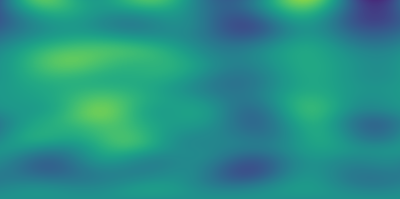
\includegraphics[interpolate=false,width=1.000000in,height=1.000000in]{burgers_rollout_diff_0.0-img0.png}}%
\end{pgfscope}%
\begin{pgfscope}%
\pgfsetbuttcap%
\pgfsetroundjoin%
\definecolor{currentfill}{rgb}{0.000000,0.000000,0.000000}%
\pgfsetfillcolor{currentfill}%
\pgfsetlinewidth{0.803000pt}%
\definecolor{currentstroke}{rgb}{0.000000,0.000000,0.000000}%
\pgfsetstrokecolor{currentstroke}%
\pgfsetdash{}{0pt}%
\pgfsys@defobject{currentmarker}{\pgfqpoint{0.000000in}{-0.048611in}}{\pgfqpoint{0.000000in}{0.000000in}}{%
\pgfpathmoveto{\pgfqpoint{0.000000in}{0.000000in}}%
\pgfpathlineto{\pgfqpoint{0.000000in}{-0.048611in}}%
\pgfusepath{stroke,fill}%
}%
\begin{pgfscope}%
\pgfsys@transformshift{0.726837in}{0.517039in}%
\pgfsys@useobject{currentmarker}{}%
\end{pgfscope}%
\end{pgfscope}%
\begin{pgfscope}%
\definecolor{textcolor}{rgb}{0.000000,0.000000,0.000000}%
\pgfsetstrokecolor{textcolor}%
\pgfsetfillcolor{textcolor}%
\pgftext[x=0.726837in,y=0.419816in,,top]{\color{textcolor}{\rmfamily\fontsize{12.000000}{14.400000}\selectfont\catcode`\^=\active\def^{\ifmmode\sp\else\^{}\fi}\catcode`\%=\active\def%{\%}0}}%
\end{pgfscope}%
\begin{pgfscope}%
\pgfsetbuttcap%
\pgfsetroundjoin%
\definecolor{currentfill}{rgb}{0.000000,0.000000,0.000000}%
\pgfsetfillcolor{currentfill}%
\pgfsetlinewidth{0.803000pt}%
\definecolor{currentstroke}{rgb}{0.000000,0.000000,0.000000}%
\pgfsetstrokecolor{currentstroke}%
\pgfsetdash{}{0pt}%
\pgfsys@defobject{currentmarker}{\pgfqpoint{0.000000in}{-0.048611in}}{\pgfqpoint{0.000000in}{0.000000in}}{%
\pgfpathmoveto{\pgfqpoint{0.000000in}{0.000000in}}%
\pgfpathlineto{\pgfqpoint{0.000000in}{-0.048611in}}%
\pgfusepath{stroke,fill}%
}%
\begin{pgfscope}%
\pgfsys@transformshift{1.570762in}{0.517039in}%
\pgfsys@useobject{currentmarker}{}%
\end{pgfscope}%
\end{pgfscope}%
\begin{pgfscope}%
\definecolor{textcolor}{rgb}{0.000000,0.000000,0.000000}%
\pgfsetstrokecolor{textcolor}%
\pgfsetfillcolor{textcolor}%
\pgftext[x=1.570762in,y=0.419816in,,top]{\color{textcolor}{\rmfamily\fontsize{12.000000}{14.400000}\selectfont\catcode`\^=\active\def^{\ifmmode\sp\else\^{}\fi}\catcode`\%=\active\def%{\%}1}}%
\end{pgfscope}%
\begin{pgfscope}%
\pgfsetbuttcap%
\pgfsetroundjoin%
\definecolor{currentfill}{rgb}{0.000000,0.000000,0.000000}%
\pgfsetfillcolor{currentfill}%
\pgfsetlinewidth{0.803000pt}%
\definecolor{currentstroke}{rgb}{0.000000,0.000000,0.000000}%
\pgfsetstrokecolor{currentstroke}%
\pgfsetdash{}{0pt}%
\pgfsys@defobject{currentmarker}{\pgfqpoint{0.000000in}{-0.048611in}}{\pgfqpoint{0.000000in}{0.000000in}}{%
\pgfpathmoveto{\pgfqpoint{0.000000in}{0.000000in}}%
\pgfpathlineto{\pgfqpoint{0.000000in}{-0.048611in}}%
\pgfusepath{stroke,fill}%
}%
\begin{pgfscope}%
\pgfsys@transformshift{2.414687in}{0.517039in}%
\pgfsys@useobject{currentmarker}{}%
\end{pgfscope}%
\end{pgfscope}%
\begin{pgfscope}%
\definecolor{textcolor}{rgb}{0.000000,0.000000,0.000000}%
\pgfsetstrokecolor{textcolor}%
\pgfsetfillcolor{textcolor}%
\pgftext[x=2.414687in,y=0.419816in,,top]{\color{textcolor}{\rmfamily\fontsize{12.000000}{14.400000}\selectfont\catcode`\^=\active\def^{\ifmmode\sp\else\^{}\fi}\catcode`\%=\active\def%{\%}2}}%
\end{pgfscope}%
\begin{pgfscope}%
\definecolor{textcolor}{rgb}{0.000000,0.000000,0.000000}%
\pgfsetstrokecolor{textcolor}%
\pgfsetfillcolor{textcolor}%
\pgftext[x=1.570762in,y=0.202965in,,top]{\color{textcolor}{\rmfamily\fontsize{12.000000}{14.400000}\selectfont\catcode`\^=\active\def^{\ifmmode\sp\else\^{}\fi}\catcode`\%=\active\def%{\%}Space}}%
\end{pgfscope}%
\begin{pgfscope}%
\pgfsetbuttcap%
\pgfsetroundjoin%
\definecolor{currentfill}{rgb}{0.000000,0.000000,0.000000}%
\pgfsetfillcolor{currentfill}%
\pgfsetlinewidth{0.803000pt}%
\definecolor{currentstroke}{rgb}{0.000000,0.000000,0.000000}%
\pgfsetstrokecolor{currentstroke}%
\pgfsetdash{}{0pt}%
\pgfsys@defobject{currentmarker}{\pgfqpoint{-0.048611in}{0.000000in}}{\pgfqpoint{-0.000000in}{0.000000in}}{%
\pgfpathmoveto{\pgfqpoint{-0.000000in}{0.000000in}}%
\pgfpathlineto{\pgfqpoint{-0.048611in}{0.000000in}}%
\pgfusepath{stroke,fill}%
}%
\begin{pgfscope}%
\pgfsys@transformshift{0.726837in}{0.517039in}%
\pgfsys@useobject{currentmarker}{}%
\end{pgfscope}%
\end{pgfscope}%
\begin{pgfscope}%
\definecolor{textcolor}{rgb}{0.000000,0.000000,0.000000}%
\pgfsetstrokecolor{textcolor}%
\pgfsetfillcolor{textcolor}%
\pgftext[x=0.364559in, y=0.453725in, left, base]{\color{textcolor}{\rmfamily\fontsize{12.000000}{14.400000}\selectfont\catcode`\^=\active\def^{\ifmmode\sp\else\^{}\fi}\catcode`\%=\active\def%{\%}0.0}}%
\end{pgfscope}%
\begin{pgfscope}%
\pgfsetbuttcap%
\pgfsetroundjoin%
\definecolor{currentfill}{rgb}{0.000000,0.000000,0.000000}%
\pgfsetfillcolor{currentfill}%
\pgfsetlinewidth{0.803000pt}%
\definecolor{currentstroke}{rgb}{0.000000,0.000000,0.000000}%
\pgfsetstrokecolor{currentstroke}%
\pgfsetdash{}{0pt}%
\pgfsys@defobject{currentmarker}{\pgfqpoint{-0.048611in}{0.000000in}}{\pgfqpoint{-0.000000in}{0.000000in}}{%
\pgfpathmoveto{\pgfqpoint{-0.000000in}{0.000000in}}%
\pgfpathlineto{\pgfqpoint{-0.048611in}{0.000000in}}%
\pgfusepath{stroke,fill}%
}%
\begin{pgfscope}%
\pgfsys@transformshift{0.726837in}{0.861533in}%
\pgfsys@useobject{currentmarker}{}%
\end{pgfscope}%
\end{pgfscope}%
\begin{pgfscope}%
\definecolor{textcolor}{rgb}{0.000000,0.000000,0.000000}%
\pgfsetstrokecolor{textcolor}%
\pgfsetfillcolor{textcolor}%
\pgftext[x=0.364559in, y=0.798219in, left, base]{\color{textcolor}{\rmfamily\fontsize{12.000000}{14.400000}\selectfont\catcode`\^=\active\def^{\ifmmode\sp\else\^{}\fi}\catcode`\%=\active\def%{\%}2.5}}%
\end{pgfscope}%
\begin{pgfscope}%
\pgfsetbuttcap%
\pgfsetroundjoin%
\definecolor{currentfill}{rgb}{0.000000,0.000000,0.000000}%
\pgfsetfillcolor{currentfill}%
\pgfsetlinewidth{0.803000pt}%
\definecolor{currentstroke}{rgb}{0.000000,0.000000,0.000000}%
\pgfsetstrokecolor{currentstroke}%
\pgfsetdash{}{0pt}%
\pgfsys@defobject{currentmarker}{\pgfqpoint{-0.048611in}{0.000000in}}{\pgfqpoint{-0.000000in}{0.000000in}}{%
\pgfpathmoveto{\pgfqpoint{-0.000000in}{0.000000in}}%
\pgfpathlineto{\pgfqpoint{-0.048611in}{0.000000in}}%
\pgfusepath{stroke,fill}%
}%
\begin{pgfscope}%
\pgfsys@transformshift{0.726837in}{1.206027in}%
\pgfsys@useobject{currentmarker}{}%
\end{pgfscope}%
\end{pgfscope}%
\begin{pgfscope}%
\definecolor{textcolor}{rgb}{0.000000,0.000000,0.000000}%
\pgfsetstrokecolor{textcolor}%
\pgfsetfillcolor{textcolor}%
\pgftext[x=0.364559in, y=1.142714in, left, base]{\color{textcolor}{\rmfamily\fontsize{12.000000}{14.400000}\selectfont\catcode`\^=\active\def^{\ifmmode\sp\else\^{}\fi}\catcode`\%=\active\def%{\%}5.0}}%
\end{pgfscope}%
\begin{pgfscope}%
\pgfsetbuttcap%
\pgfsetroundjoin%
\definecolor{currentfill}{rgb}{0.000000,0.000000,0.000000}%
\pgfsetfillcolor{currentfill}%
\pgfsetlinewidth{0.803000pt}%
\definecolor{currentstroke}{rgb}{0.000000,0.000000,0.000000}%
\pgfsetstrokecolor{currentstroke}%
\pgfsetdash{}{0pt}%
\pgfsys@defobject{currentmarker}{\pgfqpoint{-0.048611in}{0.000000in}}{\pgfqpoint{-0.000000in}{0.000000in}}{%
\pgfpathmoveto{\pgfqpoint{-0.000000in}{0.000000in}}%
\pgfpathlineto{\pgfqpoint{-0.048611in}{0.000000in}}%
\pgfusepath{stroke,fill}%
}%
\begin{pgfscope}%
\pgfsys@transformshift{0.726837in}{1.550522in}%
\pgfsys@useobject{currentmarker}{}%
\end{pgfscope}%
\end{pgfscope}%
\begin{pgfscope}%
\definecolor{textcolor}{rgb}{0.000000,0.000000,0.000000}%
\pgfsetstrokecolor{textcolor}%
\pgfsetfillcolor{textcolor}%
\pgftext[x=0.364559in, y=1.487208in, left, base]{\color{textcolor}{\rmfamily\fontsize{12.000000}{14.400000}\selectfont\catcode`\^=\active\def^{\ifmmode\sp\else\^{}\fi}\catcode`\%=\active\def%{\%}7.5}}%
\end{pgfscope}%
\begin{pgfscope}%
\pgfsetbuttcap%
\pgfsetroundjoin%
\definecolor{currentfill}{rgb}{0.000000,0.000000,0.000000}%
\pgfsetfillcolor{currentfill}%
\pgfsetlinewidth{0.803000pt}%
\definecolor{currentstroke}{rgb}{0.000000,0.000000,0.000000}%
\pgfsetstrokecolor{currentstroke}%
\pgfsetdash{}{0pt}%
\pgfsys@defobject{currentmarker}{\pgfqpoint{-0.048611in}{0.000000in}}{\pgfqpoint{-0.000000in}{0.000000in}}{%
\pgfpathmoveto{\pgfqpoint{-0.000000in}{0.000000in}}%
\pgfpathlineto{\pgfqpoint{-0.048611in}{0.000000in}}%
\pgfusepath{stroke,fill}%
}%
\begin{pgfscope}%
\pgfsys@transformshift{0.726837in}{1.895016in}%
\pgfsys@useobject{currentmarker}{}%
\end{pgfscope}%
\end{pgfscope}%
\begin{pgfscope}%
\definecolor{textcolor}{rgb}{0.000000,0.000000,0.000000}%
\pgfsetstrokecolor{textcolor}%
\pgfsetfillcolor{textcolor}%
\pgftext[x=0.258521in, y=1.831702in, left, base]{\color{textcolor}{\rmfamily\fontsize{12.000000}{14.400000}\selectfont\catcode`\^=\active\def^{\ifmmode\sp\else\^{}\fi}\catcode`\%=\active\def%{\%}10.0}}%
\end{pgfscope}%
\begin{pgfscope}%
\definecolor{textcolor}{rgb}{0.000000,0.000000,0.000000}%
\pgfsetstrokecolor{textcolor}%
\pgfsetfillcolor{textcolor}%
\pgftext[x=0.202965in,y=1.206027in,,bottom,rotate=90.000000]{\color{textcolor}{\rmfamily\fontsize{12.000000}{14.400000}\selectfont\catcode`\^=\active\def^{\ifmmode\sp\else\^{}\fi}\catcode`\%=\active\def%{\%}Time}}%
\end{pgfscope}%
\begin{pgfscope}%
\pgfsetrectcap%
\pgfsetmiterjoin%
\pgfsetlinewidth{0.803000pt}%
\definecolor{currentstroke}{rgb}{0.000000,0.000000,0.000000}%
\pgfsetstrokecolor{currentstroke}%
\pgfsetdash{}{0pt}%
\pgfpathmoveto{\pgfqpoint{0.726837in}{0.517039in}}%
\pgfpathlineto{\pgfqpoint{0.726837in}{1.895016in}}%
\pgfusepath{stroke}%
\end{pgfscope}%
\begin{pgfscope}%
\pgfsetrectcap%
\pgfsetmiterjoin%
\pgfsetlinewidth{0.803000pt}%
\definecolor{currentstroke}{rgb}{0.000000,0.000000,0.000000}%
\pgfsetstrokecolor{currentstroke}%
\pgfsetdash{}{0pt}%
\pgfpathmoveto{\pgfqpoint{2.414687in}{0.517039in}}%
\pgfpathlineto{\pgfqpoint{2.414687in}{1.895016in}}%
\pgfusepath{stroke}%
\end{pgfscope}%
\begin{pgfscope}%
\pgfsetrectcap%
\pgfsetmiterjoin%
\pgfsetlinewidth{0.803000pt}%
\definecolor{currentstroke}{rgb}{0.000000,0.000000,0.000000}%
\pgfsetstrokecolor{currentstroke}%
\pgfsetdash{}{0pt}%
\pgfpathmoveto{\pgfqpoint{0.726837in}{0.517039in}}%
\pgfpathlineto{\pgfqpoint{2.414687in}{0.517039in}}%
\pgfusepath{stroke}%
\end{pgfscope}%
\begin{pgfscope}%
\pgfsetrectcap%
\pgfsetmiterjoin%
\pgfsetlinewidth{0.803000pt}%
\definecolor{currentstroke}{rgb}{0.000000,0.000000,0.000000}%
\pgfsetstrokecolor{currentstroke}%
\pgfsetdash{}{0pt}%
\pgfpathmoveto{\pgfqpoint{0.726837in}{1.895016in}}%
\pgfpathlineto{\pgfqpoint{2.414687in}{1.895016in}}%
\pgfusepath{stroke}%
\end{pgfscope}%
\begin{pgfscope}%
\pgfsetbuttcap%
\pgfsetmiterjoin%
\pgfsetlinewidth{0.000000pt}%
\definecolor{currentstroke}{rgb}{0.000000,0.000000,0.000000}%
\pgfsetstrokecolor{currentstroke}%
\pgfsetstrokeopacity{0.000000}%
\pgfsetdash{}{0pt}%
\pgfpathmoveto{\pgfqpoint{2.552099in}{0.517039in}}%
\pgfpathlineto{\pgfqpoint{2.620998in}{0.517039in}}%
\pgfpathlineto{\pgfqpoint{2.620998in}{1.895016in}}%
\pgfpathlineto{\pgfqpoint{2.552099in}{1.895016in}}%
\pgfpathlineto{\pgfqpoint{2.552099in}{0.517039in}}%
\pgfpathclose%
\pgfusepath{}%
\end{pgfscope}%
\begin{pgfscope}%
\pgfsys@transformshift{2.550000in}{0.520000in}%
\pgftext[left,bottom]{
\includegraphics[interpolate=true,width=0.070000in,height=1.380000in]{burgers_rollout_diff_0.0-img1.png}}%
\end{pgfscope}%
\begin{pgfscope}%
\pgfsetbuttcap%
\pgfsetroundjoin%
\definecolor{currentfill}{rgb}{0.000000,0.000000,0.000000}%
\pgfsetfillcolor{currentfill}%
\pgfsetlinewidth{0.803000pt}%
\definecolor{currentstroke}{rgb}{0.000000,0.000000,0.000000}%
\pgfsetstrokecolor{currentstroke}%
\pgfsetdash{}{0pt}%
\pgfsys@defobject{currentmarker}{\pgfqpoint{0.000000in}{0.000000in}}{\pgfqpoint{0.048611in}{0.000000in}}{%
\pgfpathmoveto{\pgfqpoint{0.000000in}{0.000000in}}%
\pgfpathlineto{\pgfqpoint{0.048611in}{0.000000in}}%
\pgfusepath{stroke,fill}%
}%
\begin{pgfscope}%
\pgfsys@transformshift{2.620998in}{0.588723in}%
\pgfsys@useobject{currentmarker}{}%
\end{pgfscope}%
\end{pgfscope}%
\begin{pgfscope}%
\definecolor{textcolor}{rgb}{0.000000,0.000000,0.000000}%
\pgfsetstrokecolor{textcolor}%
\pgfsetfillcolor{textcolor}%
\pgftext[x=2.718220in, y=0.525410in, left, base]{\color{textcolor}{\rmfamily\fontsize{12.000000}{14.400000}\selectfont\catcode`\^=\active\def^{\ifmmode\sp\else\^{}\fi}\catcode`\%=\active\def%{\%}\ensuremath{-}1}}%
\end{pgfscope}%
\begin{pgfscope}%
\pgfsetbuttcap%
\pgfsetroundjoin%
\definecolor{currentfill}{rgb}{0.000000,0.000000,0.000000}%
\pgfsetfillcolor{currentfill}%
\pgfsetlinewidth{0.803000pt}%
\definecolor{currentstroke}{rgb}{0.000000,0.000000,0.000000}%
\pgfsetstrokecolor{currentstroke}%
\pgfsetdash{}{0pt}%
\pgfsys@defobject{currentmarker}{\pgfqpoint{0.000000in}{0.000000in}}{\pgfqpoint{0.048611in}{0.000000in}}{%
\pgfpathmoveto{\pgfqpoint{0.000000in}{0.000000in}}%
\pgfpathlineto{\pgfqpoint{0.048611in}{0.000000in}}%
\pgfusepath{stroke,fill}%
}%
\begin{pgfscope}%
\pgfsys@transformshift{2.620998in}{1.206027in}%
\pgfsys@useobject{currentmarker}{}%
\end{pgfscope}%
\end{pgfscope}%
\begin{pgfscope}%
\definecolor{textcolor}{rgb}{0.000000,0.000000,0.000000}%
\pgfsetstrokecolor{textcolor}%
\pgfsetfillcolor{textcolor}%
\pgftext[x=2.718220in, y=1.142714in, left, base]{\color{textcolor}{\rmfamily\fontsize{12.000000}{14.400000}\selectfont\catcode`\^=\active\def^{\ifmmode\sp\else\^{}\fi}\catcode`\%=\active\def%{\%}0}}%
\end{pgfscope}%
\begin{pgfscope}%
\pgfsetbuttcap%
\pgfsetroundjoin%
\definecolor{currentfill}{rgb}{0.000000,0.000000,0.000000}%
\pgfsetfillcolor{currentfill}%
\pgfsetlinewidth{0.803000pt}%
\definecolor{currentstroke}{rgb}{0.000000,0.000000,0.000000}%
\pgfsetstrokecolor{currentstroke}%
\pgfsetdash{}{0pt}%
\pgfsys@defobject{currentmarker}{\pgfqpoint{0.000000in}{0.000000in}}{\pgfqpoint{0.048611in}{0.000000in}}{%
\pgfpathmoveto{\pgfqpoint{0.000000in}{0.000000in}}%
\pgfpathlineto{\pgfqpoint{0.048611in}{0.000000in}}%
\pgfusepath{stroke,fill}%
}%
\begin{pgfscope}%
\pgfsys@transformshift{2.620998in}{1.823331in}%
\pgfsys@useobject{currentmarker}{}%
\end{pgfscope}%
\end{pgfscope}%
\begin{pgfscope}%
\definecolor{textcolor}{rgb}{0.000000,0.000000,0.000000}%
\pgfsetstrokecolor{textcolor}%
\pgfsetfillcolor{textcolor}%
\pgftext[x=2.718220in, y=1.760018in, left, base]{\color{textcolor}{\rmfamily\fontsize{12.000000}{14.400000}\selectfont\catcode`\^=\active\def^{\ifmmode\sp\else\^{}\fi}\catcode`\%=\active\def%{\%}1}}%
\end{pgfscope}%
\begin{pgfscope}%
\pgfsetrectcap%
\pgfsetmiterjoin%
\pgfsetlinewidth{0.803000pt}%
\definecolor{currentstroke}{rgb}{0.000000,0.000000,0.000000}%
\pgfsetstrokecolor{currentstroke}%
\pgfsetdash{}{0pt}%
\pgfpathmoveto{\pgfqpoint{2.552099in}{0.517039in}}%
\pgfpathlineto{\pgfqpoint{2.586548in}{0.517039in}}%
\pgfpathlineto{\pgfqpoint{2.620998in}{0.517039in}}%
\pgfpathlineto{\pgfqpoint{2.620998in}{1.895016in}}%
\pgfpathlineto{\pgfqpoint{2.586548in}{1.895016in}}%
\pgfpathlineto{\pgfqpoint{2.552099in}{1.895016in}}%
\pgfpathlineto{\pgfqpoint{2.552099in}{0.517039in}}%
\pgfpathclose%
\pgfusepath{stroke}%
\end{pgfscope}%
\end{pgfpicture}%
\makeatother%
\endgroup%

      \end{adjustbox}
      \caption{The difference for \(\nu=0.0\)}\label{fig:sc2_rollout_diff_0.0}
    \end{subfigure}
    \\[0.7\baselineskip]
    \begin{subfigure}{0.33\linewidth}
      \begin{adjustbox}{width=\linewidth}
        \begingroup%
\makeatletter%
\begin{pgfpicture}%
\pgfpathrectangle{\pgfpointorigin}{\pgfqpoint{3.000000in}{2.000000in}}%
\pgfusepath{use as bounding box, clip}%
\begin{pgfscope}%
\pgfsetbuttcap%
\pgfsetmiterjoin%
\pgfsetlinewidth{0.000000pt}%
\definecolor{currentstroke}{rgb}{0.000000,0.000000,0.000000}%
\pgfsetstrokecolor{currentstroke}%
\pgfsetstrokeopacity{0.000000}%
\pgfsetdash{}{0pt}%
\pgfpathmoveto{\pgfqpoint{0.000000in}{0.000000in}}%
\pgfpathlineto{\pgfqpoint{3.000000in}{0.000000in}}%
\pgfpathlineto{\pgfqpoint{3.000000in}{2.000000in}}%
\pgfpathlineto{\pgfqpoint{0.000000in}{2.000000in}}%
\pgfpathlineto{\pgfqpoint{0.000000in}{0.000000in}}%
\pgfpathclose%
\pgfusepath{}%
\end{pgfscope}%
\begin{pgfscope}%
\pgfsetbuttcap%
\pgfsetmiterjoin%
\pgfsetlinewidth{0.000000pt}%
\definecolor{currentstroke}{rgb}{0.000000,0.000000,0.000000}%
\pgfsetstrokecolor{currentstroke}%
\pgfsetstrokeopacity{0.000000}%
\pgfsetdash{}{0pt}%
\pgfpathmoveto{\pgfqpoint{0.726837in}{0.517039in}}%
\pgfpathlineto{\pgfqpoint{2.414687in}{0.517039in}}%
\pgfpathlineto{\pgfqpoint{2.414687in}{1.895016in}}%
\pgfpathlineto{\pgfqpoint{0.726837in}{1.895016in}}%
\pgfpathlineto{\pgfqpoint{0.726837in}{0.517039in}}%
\pgfpathclose%
\pgfusepath{}%
\end{pgfscope}%
\begin{pgfscope}%
\pgfpathrectangle{\pgfqpoint{0.726837in}{0.517039in}}{\pgfqpoint{1.687850in}{1.377978in}}%
\pgfusepath{clip}%
\pgfsys@transformcm{1.687850}{0.000000}{0.000000}{1.377978}{0.726837in}{0.517039in}%
\pgftext[left,bottom]{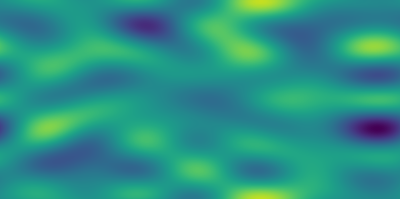
\includegraphics[interpolate=false,width=1.000000in,height=1.000000in]{burgers_rollout_target_0.01-img0.png}}%
\end{pgfscope}%
\begin{pgfscope}%
\pgfsetbuttcap%
\pgfsetroundjoin%
\definecolor{currentfill}{rgb}{0.000000,0.000000,0.000000}%
\pgfsetfillcolor{currentfill}%
\pgfsetlinewidth{0.803000pt}%
\definecolor{currentstroke}{rgb}{0.000000,0.000000,0.000000}%
\pgfsetstrokecolor{currentstroke}%
\pgfsetdash{}{0pt}%
\pgfsys@defobject{currentmarker}{\pgfqpoint{0.000000in}{-0.048611in}}{\pgfqpoint{0.000000in}{0.000000in}}{%
\pgfpathmoveto{\pgfqpoint{0.000000in}{0.000000in}}%
\pgfpathlineto{\pgfqpoint{0.000000in}{-0.048611in}}%
\pgfusepath{stroke,fill}%
}%
\begin{pgfscope}%
\pgfsys@transformshift{0.726837in}{0.517039in}%
\pgfsys@useobject{currentmarker}{}%
\end{pgfscope}%
\end{pgfscope}%
\begin{pgfscope}%
\definecolor{textcolor}{rgb}{0.000000,0.000000,0.000000}%
\pgfsetstrokecolor{textcolor}%
\pgfsetfillcolor{textcolor}%
\pgftext[x=0.726837in,y=0.419816in,,top]{\color{textcolor}\rmfamily\fontsize{12.000000}{14.400000}\selectfont 0}%
\end{pgfscope}%
\begin{pgfscope}%
\pgfsetbuttcap%
\pgfsetroundjoin%
\definecolor{currentfill}{rgb}{0.000000,0.000000,0.000000}%
\pgfsetfillcolor{currentfill}%
\pgfsetlinewidth{0.803000pt}%
\definecolor{currentstroke}{rgb}{0.000000,0.000000,0.000000}%
\pgfsetstrokecolor{currentstroke}%
\pgfsetdash{}{0pt}%
\pgfsys@defobject{currentmarker}{\pgfqpoint{0.000000in}{-0.048611in}}{\pgfqpoint{0.000000in}{0.000000in}}{%
\pgfpathmoveto{\pgfqpoint{0.000000in}{0.000000in}}%
\pgfpathlineto{\pgfqpoint{0.000000in}{-0.048611in}}%
\pgfusepath{stroke,fill}%
}%
\begin{pgfscope}%
\pgfsys@transformshift{1.570762in}{0.517039in}%
\pgfsys@useobject{currentmarker}{}%
\end{pgfscope}%
\end{pgfscope}%
\begin{pgfscope}%
\definecolor{textcolor}{rgb}{0.000000,0.000000,0.000000}%
\pgfsetstrokecolor{textcolor}%
\pgfsetfillcolor{textcolor}%
\pgftext[x=1.570762in,y=0.419816in,,top]{\color{textcolor}\rmfamily\fontsize{12.000000}{14.400000}\selectfont 1}%
\end{pgfscope}%
\begin{pgfscope}%
\pgfsetbuttcap%
\pgfsetroundjoin%
\definecolor{currentfill}{rgb}{0.000000,0.000000,0.000000}%
\pgfsetfillcolor{currentfill}%
\pgfsetlinewidth{0.803000pt}%
\definecolor{currentstroke}{rgb}{0.000000,0.000000,0.000000}%
\pgfsetstrokecolor{currentstroke}%
\pgfsetdash{}{0pt}%
\pgfsys@defobject{currentmarker}{\pgfqpoint{0.000000in}{-0.048611in}}{\pgfqpoint{0.000000in}{0.000000in}}{%
\pgfpathmoveto{\pgfqpoint{0.000000in}{0.000000in}}%
\pgfpathlineto{\pgfqpoint{0.000000in}{-0.048611in}}%
\pgfusepath{stroke,fill}%
}%
\begin{pgfscope}%
\pgfsys@transformshift{2.414687in}{0.517039in}%
\pgfsys@useobject{currentmarker}{}%
\end{pgfscope}%
\end{pgfscope}%
\begin{pgfscope}%
\definecolor{textcolor}{rgb}{0.000000,0.000000,0.000000}%
\pgfsetstrokecolor{textcolor}%
\pgfsetfillcolor{textcolor}%
\pgftext[x=2.414687in,y=0.419816in,,top]{\color{textcolor}\rmfamily\fontsize{12.000000}{14.400000}\selectfont 2}%
\end{pgfscope}%
\begin{pgfscope}%
\definecolor{textcolor}{rgb}{0.000000,0.000000,0.000000}%
\pgfsetstrokecolor{textcolor}%
\pgfsetfillcolor{textcolor}%
\pgftext[x=1.570762in,y=0.202965in,,top]{\color{textcolor}\rmfamily\fontsize{12.000000}{14.400000}\selectfont Space}%
\end{pgfscope}%
\begin{pgfscope}%
\pgfsetbuttcap%
\pgfsetroundjoin%
\definecolor{currentfill}{rgb}{0.000000,0.000000,0.000000}%
\pgfsetfillcolor{currentfill}%
\pgfsetlinewidth{0.803000pt}%
\definecolor{currentstroke}{rgb}{0.000000,0.000000,0.000000}%
\pgfsetstrokecolor{currentstroke}%
\pgfsetdash{}{0pt}%
\pgfsys@defobject{currentmarker}{\pgfqpoint{-0.048611in}{0.000000in}}{\pgfqpoint{-0.000000in}{0.000000in}}{%
\pgfpathmoveto{\pgfqpoint{-0.000000in}{0.000000in}}%
\pgfpathlineto{\pgfqpoint{-0.048611in}{0.000000in}}%
\pgfusepath{stroke,fill}%
}%
\begin{pgfscope}%
\pgfsys@transformshift{0.726837in}{0.517039in}%
\pgfsys@useobject{currentmarker}{}%
\end{pgfscope}%
\end{pgfscope}%
\begin{pgfscope}%
\definecolor{textcolor}{rgb}{0.000000,0.000000,0.000000}%
\pgfsetstrokecolor{textcolor}%
\pgfsetfillcolor{textcolor}%
\pgftext[x=0.364559in, y=0.453725in, left, base]{\color{textcolor}\rmfamily\fontsize{12.000000}{14.400000}\selectfont 0.0}%
\end{pgfscope}%
\begin{pgfscope}%
\pgfsetbuttcap%
\pgfsetroundjoin%
\definecolor{currentfill}{rgb}{0.000000,0.000000,0.000000}%
\pgfsetfillcolor{currentfill}%
\pgfsetlinewidth{0.803000pt}%
\definecolor{currentstroke}{rgb}{0.000000,0.000000,0.000000}%
\pgfsetstrokecolor{currentstroke}%
\pgfsetdash{}{0pt}%
\pgfsys@defobject{currentmarker}{\pgfqpoint{-0.048611in}{0.000000in}}{\pgfqpoint{-0.000000in}{0.000000in}}{%
\pgfpathmoveto{\pgfqpoint{-0.000000in}{0.000000in}}%
\pgfpathlineto{\pgfqpoint{-0.048611in}{0.000000in}}%
\pgfusepath{stroke,fill}%
}%
\begin{pgfscope}%
\pgfsys@transformshift{0.726837in}{0.861533in}%
\pgfsys@useobject{currentmarker}{}%
\end{pgfscope}%
\end{pgfscope}%
\begin{pgfscope}%
\definecolor{textcolor}{rgb}{0.000000,0.000000,0.000000}%
\pgfsetstrokecolor{textcolor}%
\pgfsetfillcolor{textcolor}%
\pgftext[x=0.364559in, y=0.798219in, left, base]{\color{textcolor}\rmfamily\fontsize{12.000000}{14.400000}\selectfont 2.5}%
\end{pgfscope}%
\begin{pgfscope}%
\pgfsetbuttcap%
\pgfsetroundjoin%
\definecolor{currentfill}{rgb}{0.000000,0.000000,0.000000}%
\pgfsetfillcolor{currentfill}%
\pgfsetlinewidth{0.803000pt}%
\definecolor{currentstroke}{rgb}{0.000000,0.000000,0.000000}%
\pgfsetstrokecolor{currentstroke}%
\pgfsetdash{}{0pt}%
\pgfsys@defobject{currentmarker}{\pgfqpoint{-0.048611in}{0.000000in}}{\pgfqpoint{-0.000000in}{0.000000in}}{%
\pgfpathmoveto{\pgfqpoint{-0.000000in}{0.000000in}}%
\pgfpathlineto{\pgfqpoint{-0.048611in}{0.000000in}}%
\pgfusepath{stroke,fill}%
}%
\begin{pgfscope}%
\pgfsys@transformshift{0.726837in}{1.206027in}%
\pgfsys@useobject{currentmarker}{}%
\end{pgfscope}%
\end{pgfscope}%
\begin{pgfscope}%
\definecolor{textcolor}{rgb}{0.000000,0.000000,0.000000}%
\pgfsetstrokecolor{textcolor}%
\pgfsetfillcolor{textcolor}%
\pgftext[x=0.364559in, y=1.142714in, left, base]{\color{textcolor}\rmfamily\fontsize{12.000000}{14.400000}\selectfont 5.0}%
\end{pgfscope}%
\begin{pgfscope}%
\pgfsetbuttcap%
\pgfsetroundjoin%
\definecolor{currentfill}{rgb}{0.000000,0.000000,0.000000}%
\pgfsetfillcolor{currentfill}%
\pgfsetlinewidth{0.803000pt}%
\definecolor{currentstroke}{rgb}{0.000000,0.000000,0.000000}%
\pgfsetstrokecolor{currentstroke}%
\pgfsetdash{}{0pt}%
\pgfsys@defobject{currentmarker}{\pgfqpoint{-0.048611in}{0.000000in}}{\pgfqpoint{-0.000000in}{0.000000in}}{%
\pgfpathmoveto{\pgfqpoint{-0.000000in}{0.000000in}}%
\pgfpathlineto{\pgfqpoint{-0.048611in}{0.000000in}}%
\pgfusepath{stroke,fill}%
}%
\begin{pgfscope}%
\pgfsys@transformshift{0.726837in}{1.550522in}%
\pgfsys@useobject{currentmarker}{}%
\end{pgfscope}%
\end{pgfscope}%
\begin{pgfscope}%
\definecolor{textcolor}{rgb}{0.000000,0.000000,0.000000}%
\pgfsetstrokecolor{textcolor}%
\pgfsetfillcolor{textcolor}%
\pgftext[x=0.364559in, y=1.487208in, left, base]{\color{textcolor}\rmfamily\fontsize{12.000000}{14.400000}\selectfont 7.5}%
\end{pgfscope}%
\begin{pgfscope}%
\pgfsetbuttcap%
\pgfsetroundjoin%
\definecolor{currentfill}{rgb}{0.000000,0.000000,0.000000}%
\pgfsetfillcolor{currentfill}%
\pgfsetlinewidth{0.803000pt}%
\definecolor{currentstroke}{rgb}{0.000000,0.000000,0.000000}%
\pgfsetstrokecolor{currentstroke}%
\pgfsetdash{}{0pt}%
\pgfsys@defobject{currentmarker}{\pgfqpoint{-0.048611in}{0.000000in}}{\pgfqpoint{-0.000000in}{0.000000in}}{%
\pgfpathmoveto{\pgfqpoint{-0.000000in}{0.000000in}}%
\pgfpathlineto{\pgfqpoint{-0.048611in}{0.000000in}}%
\pgfusepath{stroke,fill}%
}%
\begin{pgfscope}%
\pgfsys@transformshift{0.726837in}{1.895016in}%
\pgfsys@useobject{currentmarker}{}%
\end{pgfscope}%
\end{pgfscope}%
\begin{pgfscope}%
\definecolor{textcolor}{rgb}{0.000000,0.000000,0.000000}%
\pgfsetstrokecolor{textcolor}%
\pgfsetfillcolor{textcolor}%
\pgftext[x=0.258521in, y=1.831702in, left, base]{\color{textcolor}\rmfamily\fontsize{12.000000}{14.400000}\selectfont 10.0}%
\end{pgfscope}%
\begin{pgfscope}%
\definecolor{textcolor}{rgb}{0.000000,0.000000,0.000000}%
\pgfsetstrokecolor{textcolor}%
\pgfsetfillcolor{textcolor}%
\pgftext[x=0.202965in,y=1.206027in,,bottom,rotate=90.000000]{\color{textcolor}\rmfamily\fontsize{12.000000}{14.400000}\selectfont Time}%
\end{pgfscope}%
\begin{pgfscope}%
\pgfsetrectcap%
\pgfsetmiterjoin%
\pgfsetlinewidth{0.803000pt}%
\definecolor{currentstroke}{rgb}{0.000000,0.000000,0.000000}%
\pgfsetstrokecolor{currentstroke}%
\pgfsetdash{}{0pt}%
\pgfpathmoveto{\pgfqpoint{0.726837in}{0.517039in}}%
\pgfpathlineto{\pgfqpoint{0.726837in}{1.895016in}}%
\pgfusepath{stroke}%
\end{pgfscope}%
\begin{pgfscope}%
\pgfsetrectcap%
\pgfsetmiterjoin%
\pgfsetlinewidth{0.803000pt}%
\definecolor{currentstroke}{rgb}{0.000000,0.000000,0.000000}%
\pgfsetstrokecolor{currentstroke}%
\pgfsetdash{}{0pt}%
\pgfpathmoveto{\pgfqpoint{2.414687in}{0.517039in}}%
\pgfpathlineto{\pgfqpoint{2.414687in}{1.895016in}}%
\pgfusepath{stroke}%
\end{pgfscope}%
\begin{pgfscope}%
\pgfsetrectcap%
\pgfsetmiterjoin%
\pgfsetlinewidth{0.803000pt}%
\definecolor{currentstroke}{rgb}{0.000000,0.000000,0.000000}%
\pgfsetstrokecolor{currentstroke}%
\pgfsetdash{}{0pt}%
\pgfpathmoveto{\pgfqpoint{0.726837in}{0.517039in}}%
\pgfpathlineto{\pgfqpoint{2.414687in}{0.517039in}}%
\pgfusepath{stroke}%
\end{pgfscope}%
\begin{pgfscope}%
\pgfsetrectcap%
\pgfsetmiterjoin%
\pgfsetlinewidth{0.803000pt}%
\definecolor{currentstroke}{rgb}{0.000000,0.000000,0.000000}%
\pgfsetstrokecolor{currentstroke}%
\pgfsetdash{}{0pt}%
\pgfpathmoveto{\pgfqpoint{0.726837in}{1.895016in}}%
\pgfpathlineto{\pgfqpoint{2.414687in}{1.895016in}}%
\pgfusepath{stroke}%
\end{pgfscope}%
\begin{pgfscope}%
\pgfsetbuttcap%
\pgfsetmiterjoin%
\pgfsetlinewidth{0.000000pt}%
\definecolor{currentstroke}{rgb}{0.000000,0.000000,0.000000}%
\pgfsetstrokecolor{currentstroke}%
\pgfsetstrokeopacity{0.000000}%
\pgfsetdash{}{0pt}%
\pgfpathmoveto{\pgfqpoint{2.552099in}{0.517039in}}%
\pgfpathlineto{\pgfqpoint{2.620998in}{0.517039in}}%
\pgfpathlineto{\pgfqpoint{2.620998in}{1.895016in}}%
\pgfpathlineto{\pgfqpoint{2.552099in}{1.895016in}}%
\pgfpathlineto{\pgfqpoint{2.552099in}{0.517039in}}%
\pgfpathclose%
\pgfusepath{}%
\end{pgfscope}%
\begin{pgfscope}%
\pgfsys@transformshift{2.550000in}{0.520000in}%
\pgftext[left,bottom]{
\includegraphics[interpolate=true,width=0.070000in,height=1.380000in]{burgers_rollout_target_0.01-img1.png}}%
\end{pgfscope}%
\begin{pgfscope}%
\pgfsetbuttcap%
\pgfsetroundjoin%
\definecolor{currentfill}{rgb}{0.000000,0.000000,0.000000}%
\pgfsetfillcolor{currentfill}%
\pgfsetlinewidth{0.803000pt}%
\definecolor{currentstroke}{rgb}{0.000000,0.000000,0.000000}%
\pgfsetstrokecolor{currentstroke}%
\pgfsetdash{}{0pt}%
\pgfsys@defobject{currentmarker}{\pgfqpoint{0.000000in}{0.000000in}}{\pgfqpoint{0.048611in}{0.000000in}}{%
\pgfpathmoveto{\pgfqpoint{0.000000in}{0.000000in}}%
\pgfpathlineto{\pgfqpoint{0.048611in}{0.000000in}}%
\pgfusepath{stroke,fill}%
}%
\begin{pgfscope}%
\pgfsys@transformshift{2.620998in}{0.588723in}%
\pgfsys@useobject{currentmarker}{}%
\end{pgfscope}%
\end{pgfscope}%
\begin{pgfscope}%
\definecolor{textcolor}{rgb}{0.000000,0.000000,0.000000}%
\pgfsetstrokecolor{textcolor}%
\pgfsetfillcolor{textcolor}%
\pgftext[x=2.718220in, y=0.525410in, left, base]{\color{textcolor}\rmfamily\fontsize{12.000000}{14.400000}\selectfont \ensuremath{-}1}%
\end{pgfscope}%
\begin{pgfscope}%
\pgfsetbuttcap%
\pgfsetroundjoin%
\definecolor{currentfill}{rgb}{0.000000,0.000000,0.000000}%
\pgfsetfillcolor{currentfill}%
\pgfsetlinewidth{0.803000pt}%
\definecolor{currentstroke}{rgb}{0.000000,0.000000,0.000000}%
\pgfsetstrokecolor{currentstroke}%
\pgfsetdash{}{0pt}%
\pgfsys@defobject{currentmarker}{\pgfqpoint{0.000000in}{0.000000in}}{\pgfqpoint{0.048611in}{0.000000in}}{%
\pgfpathmoveto{\pgfqpoint{0.000000in}{0.000000in}}%
\pgfpathlineto{\pgfqpoint{0.048611in}{0.000000in}}%
\pgfusepath{stroke,fill}%
}%
\begin{pgfscope}%
\pgfsys@transformshift{2.620998in}{1.206027in}%
\pgfsys@useobject{currentmarker}{}%
\end{pgfscope}%
\end{pgfscope}%
\begin{pgfscope}%
\definecolor{textcolor}{rgb}{0.000000,0.000000,0.000000}%
\pgfsetstrokecolor{textcolor}%
\pgfsetfillcolor{textcolor}%
\pgftext[x=2.718220in, y=1.142714in, left, base]{\color{textcolor}\rmfamily\fontsize{12.000000}{14.400000}\selectfont 0}%
\end{pgfscope}%
\begin{pgfscope}%
\pgfsetbuttcap%
\pgfsetroundjoin%
\definecolor{currentfill}{rgb}{0.000000,0.000000,0.000000}%
\pgfsetfillcolor{currentfill}%
\pgfsetlinewidth{0.803000pt}%
\definecolor{currentstroke}{rgb}{0.000000,0.000000,0.000000}%
\pgfsetstrokecolor{currentstroke}%
\pgfsetdash{}{0pt}%
\pgfsys@defobject{currentmarker}{\pgfqpoint{0.000000in}{0.000000in}}{\pgfqpoint{0.048611in}{0.000000in}}{%
\pgfpathmoveto{\pgfqpoint{0.000000in}{0.000000in}}%
\pgfpathlineto{\pgfqpoint{0.048611in}{0.000000in}}%
\pgfusepath{stroke,fill}%
}%
\begin{pgfscope}%
\pgfsys@transformshift{2.620998in}{1.823331in}%
\pgfsys@useobject{currentmarker}{}%
\end{pgfscope}%
\end{pgfscope}%
\begin{pgfscope}%
\definecolor{textcolor}{rgb}{0.000000,0.000000,0.000000}%
\pgfsetstrokecolor{textcolor}%
\pgfsetfillcolor{textcolor}%
\pgftext[x=2.718220in, y=1.760018in, left, base]{\color{textcolor}\rmfamily\fontsize{12.000000}{14.400000}\selectfont 1}%
\end{pgfscope}%
\begin{pgfscope}%
\pgfsetrectcap%
\pgfsetmiterjoin%
\pgfsetlinewidth{0.803000pt}%
\definecolor{currentstroke}{rgb}{0.000000,0.000000,0.000000}%
\pgfsetstrokecolor{currentstroke}%
\pgfsetdash{}{0pt}%
\pgfpathmoveto{\pgfqpoint{2.552099in}{0.517039in}}%
\pgfpathlineto{\pgfqpoint{2.586548in}{0.517039in}}%
\pgfpathlineto{\pgfqpoint{2.620998in}{0.517039in}}%
\pgfpathlineto{\pgfqpoint{2.620998in}{1.895016in}}%
\pgfpathlineto{\pgfqpoint{2.586548in}{1.895016in}}%
\pgfpathlineto{\pgfqpoint{2.552099in}{1.895016in}}%
\pgfpathlineto{\pgfqpoint{2.552099in}{0.517039in}}%
\pgfpathclose%
\pgfusepath{stroke}%
\end{pgfscope}%
\end{pgfpicture}%
\makeatother%
\endgroup%

      \end{adjustbox}
      \caption{The target for \(\nu=0.01\)}\label{fig:sc2_rollout_target_0.01}
    \end{subfigure}
    \begin{subfigure}{0.33\linewidth}
      \begin{adjustbox}{width=\linewidth}
        \begingroup%
\makeatletter%
\begin{pgfpicture}%
\pgfpathrectangle{\pgfpointorigin}{\pgfqpoint{3.000000in}{2.000000in}}%
\pgfusepath{use as bounding box, clip}%
\begin{pgfscope}%
\pgfsetbuttcap%
\pgfsetmiterjoin%
\pgfsetlinewidth{0.000000pt}%
\definecolor{currentstroke}{rgb}{0.000000,0.000000,0.000000}%
\pgfsetstrokecolor{currentstroke}%
\pgfsetstrokeopacity{0.000000}%
\pgfsetdash{}{0pt}%
\pgfpathmoveto{\pgfqpoint{0.000000in}{0.000000in}}%
\pgfpathlineto{\pgfqpoint{3.000000in}{0.000000in}}%
\pgfpathlineto{\pgfqpoint{3.000000in}{2.000000in}}%
\pgfpathlineto{\pgfqpoint{0.000000in}{2.000000in}}%
\pgfpathlineto{\pgfqpoint{0.000000in}{0.000000in}}%
\pgfpathclose%
\pgfusepath{}%
\end{pgfscope}%
\begin{pgfscope}%
\pgfsetbuttcap%
\pgfsetmiterjoin%
\pgfsetlinewidth{0.000000pt}%
\definecolor{currentstroke}{rgb}{0.000000,0.000000,0.000000}%
\pgfsetstrokecolor{currentstroke}%
\pgfsetstrokeopacity{0.000000}%
\pgfsetdash{}{0pt}%
\pgfpathmoveto{\pgfqpoint{0.726837in}{0.517039in}}%
\pgfpathlineto{\pgfqpoint{2.414687in}{0.517039in}}%
\pgfpathlineto{\pgfqpoint{2.414687in}{1.895016in}}%
\pgfpathlineto{\pgfqpoint{0.726837in}{1.895016in}}%
\pgfpathlineto{\pgfqpoint{0.726837in}{0.517039in}}%
\pgfpathclose%
\pgfusepath{}%
\end{pgfscope}%
\begin{pgfscope}%
\pgfpathrectangle{\pgfqpoint{0.726837in}{0.517039in}}{\pgfqpoint{1.687850in}{1.377978in}}%
\pgfusepath{clip}%
\pgfsys@transformcm{1.687850}{0.000000}{0.000000}{1.377978}{0.726837in}{0.517039in}%
\pgftext[left,bottom]{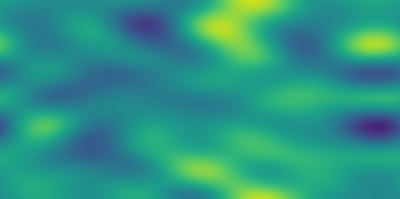
\includegraphics[interpolate=false,width=1.000000in,height=1.000000in]{burgers_rollout_pred_0.01-img0.png}}%
\end{pgfscope}%
\begin{pgfscope}%
\pgfsetbuttcap%
\pgfsetroundjoin%
\definecolor{currentfill}{rgb}{0.000000,0.000000,0.000000}%
\pgfsetfillcolor{currentfill}%
\pgfsetlinewidth{0.803000pt}%
\definecolor{currentstroke}{rgb}{0.000000,0.000000,0.000000}%
\pgfsetstrokecolor{currentstroke}%
\pgfsetdash{}{0pt}%
\pgfsys@defobject{currentmarker}{\pgfqpoint{0.000000in}{-0.048611in}}{\pgfqpoint{0.000000in}{0.000000in}}{%
\pgfpathmoveto{\pgfqpoint{0.000000in}{0.000000in}}%
\pgfpathlineto{\pgfqpoint{0.000000in}{-0.048611in}}%
\pgfusepath{stroke,fill}%
}%
\begin{pgfscope}%
\pgfsys@transformshift{0.726837in}{0.517039in}%
\pgfsys@useobject{currentmarker}{}%
\end{pgfscope}%
\end{pgfscope}%
\begin{pgfscope}%
\definecolor{textcolor}{rgb}{0.000000,0.000000,0.000000}%
\pgfsetstrokecolor{textcolor}%
\pgfsetfillcolor{textcolor}%
\pgftext[x=0.726837in,y=0.419816in,,top]{\color{textcolor}{\rmfamily\fontsize{12.000000}{14.400000}\selectfont\catcode`\^=\active\def^{\ifmmode\sp\else\^{}\fi}\catcode`\%=\active\def%{\%}0}}%
\end{pgfscope}%
\begin{pgfscope}%
\pgfsetbuttcap%
\pgfsetroundjoin%
\definecolor{currentfill}{rgb}{0.000000,0.000000,0.000000}%
\pgfsetfillcolor{currentfill}%
\pgfsetlinewidth{0.803000pt}%
\definecolor{currentstroke}{rgb}{0.000000,0.000000,0.000000}%
\pgfsetstrokecolor{currentstroke}%
\pgfsetdash{}{0pt}%
\pgfsys@defobject{currentmarker}{\pgfqpoint{0.000000in}{-0.048611in}}{\pgfqpoint{0.000000in}{0.000000in}}{%
\pgfpathmoveto{\pgfqpoint{0.000000in}{0.000000in}}%
\pgfpathlineto{\pgfqpoint{0.000000in}{-0.048611in}}%
\pgfusepath{stroke,fill}%
}%
\begin{pgfscope}%
\pgfsys@transformshift{1.570762in}{0.517039in}%
\pgfsys@useobject{currentmarker}{}%
\end{pgfscope}%
\end{pgfscope}%
\begin{pgfscope}%
\definecolor{textcolor}{rgb}{0.000000,0.000000,0.000000}%
\pgfsetstrokecolor{textcolor}%
\pgfsetfillcolor{textcolor}%
\pgftext[x=1.570762in,y=0.419816in,,top]{\color{textcolor}{\rmfamily\fontsize{12.000000}{14.400000}\selectfont\catcode`\^=\active\def^{\ifmmode\sp\else\^{}\fi}\catcode`\%=\active\def%{\%}1}}%
\end{pgfscope}%
\begin{pgfscope}%
\pgfsetbuttcap%
\pgfsetroundjoin%
\definecolor{currentfill}{rgb}{0.000000,0.000000,0.000000}%
\pgfsetfillcolor{currentfill}%
\pgfsetlinewidth{0.803000pt}%
\definecolor{currentstroke}{rgb}{0.000000,0.000000,0.000000}%
\pgfsetstrokecolor{currentstroke}%
\pgfsetdash{}{0pt}%
\pgfsys@defobject{currentmarker}{\pgfqpoint{0.000000in}{-0.048611in}}{\pgfqpoint{0.000000in}{0.000000in}}{%
\pgfpathmoveto{\pgfqpoint{0.000000in}{0.000000in}}%
\pgfpathlineto{\pgfqpoint{0.000000in}{-0.048611in}}%
\pgfusepath{stroke,fill}%
}%
\begin{pgfscope}%
\pgfsys@transformshift{2.414687in}{0.517039in}%
\pgfsys@useobject{currentmarker}{}%
\end{pgfscope}%
\end{pgfscope}%
\begin{pgfscope}%
\definecolor{textcolor}{rgb}{0.000000,0.000000,0.000000}%
\pgfsetstrokecolor{textcolor}%
\pgfsetfillcolor{textcolor}%
\pgftext[x=2.414687in,y=0.419816in,,top]{\color{textcolor}{\rmfamily\fontsize{12.000000}{14.400000}\selectfont\catcode`\^=\active\def^{\ifmmode\sp\else\^{}\fi}\catcode`\%=\active\def%{\%}2}}%
\end{pgfscope}%
\begin{pgfscope}%
\definecolor{textcolor}{rgb}{0.000000,0.000000,0.000000}%
\pgfsetstrokecolor{textcolor}%
\pgfsetfillcolor{textcolor}%
\pgftext[x=1.570762in,y=0.202965in,,top]{\color{textcolor}{\rmfamily\fontsize{12.000000}{14.400000}\selectfont\catcode`\^=\active\def^{\ifmmode\sp\else\^{}\fi}\catcode`\%=\active\def%{\%}Space}}%
\end{pgfscope}%
\begin{pgfscope}%
\pgfsetbuttcap%
\pgfsetroundjoin%
\definecolor{currentfill}{rgb}{0.000000,0.000000,0.000000}%
\pgfsetfillcolor{currentfill}%
\pgfsetlinewidth{0.803000pt}%
\definecolor{currentstroke}{rgb}{0.000000,0.000000,0.000000}%
\pgfsetstrokecolor{currentstroke}%
\pgfsetdash{}{0pt}%
\pgfsys@defobject{currentmarker}{\pgfqpoint{-0.048611in}{0.000000in}}{\pgfqpoint{-0.000000in}{0.000000in}}{%
\pgfpathmoveto{\pgfqpoint{-0.000000in}{0.000000in}}%
\pgfpathlineto{\pgfqpoint{-0.048611in}{0.000000in}}%
\pgfusepath{stroke,fill}%
}%
\begin{pgfscope}%
\pgfsys@transformshift{0.726837in}{0.517039in}%
\pgfsys@useobject{currentmarker}{}%
\end{pgfscope}%
\end{pgfscope}%
\begin{pgfscope}%
\definecolor{textcolor}{rgb}{0.000000,0.000000,0.000000}%
\pgfsetstrokecolor{textcolor}%
\pgfsetfillcolor{textcolor}%
\pgftext[x=0.364559in, y=0.453725in, left, base]{\color{textcolor}{\rmfamily\fontsize{12.000000}{14.400000}\selectfont\catcode`\^=\active\def^{\ifmmode\sp\else\^{}\fi}\catcode`\%=\active\def%{\%}0.0}}%
\end{pgfscope}%
\begin{pgfscope}%
\pgfsetbuttcap%
\pgfsetroundjoin%
\definecolor{currentfill}{rgb}{0.000000,0.000000,0.000000}%
\pgfsetfillcolor{currentfill}%
\pgfsetlinewidth{0.803000pt}%
\definecolor{currentstroke}{rgb}{0.000000,0.000000,0.000000}%
\pgfsetstrokecolor{currentstroke}%
\pgfsetdash{}{0pt}%
\pgfsys@defobject{currentmarker}{\pgfqpoint{-0.048611in}{0.000000in}}{\pgfqpoint{-0.000000in}{0.000000in}}{%
\pgfpathmoveto{\pgfqpoint{-0.000000in}{0.000000in}}%
\pgfpathlineto{\pgfqpoint{-0.048611in}{0.000000in}}%
\pgfusepath{stroke,fill}%
}%
\begin{pgfscope}%
\pgfsys@transformshift{0.726837in}{0.861533in}%
\pgfsys@useobject{currentmarker}{}%
\end{pgfscope}%
\end{pgfscope}%
\begin{pgfscope}%
\definecolor{textcolor}{rgb}{0.000000,0.000000,0.000000}%
\pgfsetstrokecolor{textcolor}%
\pgfsetfillcolor{textcolor}%
\pgftext[x=0.364559in, y=0.798219in, left, base]{\color{textcolor}{\rmfamily\fontsize{12.000000}{14.400000}\selectfont\catcode`\^=\active\def^{\ifmmode\sp\else\^{}\fi}\catcode`\%=\active\def%{\%}2.5}}%
\end{pgfscope}%
\begin{pgfscope}%
\pgfsetbuttcap%
\pgfsetroundjoin%
\definecolor{currentfill}{rgb}{0.000000,0.000000,0.000000}%
\pgfsetfillcolor{currentfill}%
\pgfsetlinewidth{0.803000pt}%
\definecolor{currentstroke}{rgb}{0.000000,0.000000,0.000000}%
\pgfsetstrokecolor{currentstroke}%
\pgfsetdash{}{0pt}%
\pgfsys@defobject{currentmarker}{\pgfqpoint{-0.048611in}{0.000000in}}{\pgfqpoint{-0.000000in}{0.000000in}}{%
\pgfpathmoveto{\pgfqpoint{-0.000000in}{0.000000in}}%
\pgfpathlineto{\pgfqpoint{-0.048611in}{0.000000in}}%
\pgfusepath{stroke,fill}%
}%
\begin{pgfscope}%
\pgfsys@transformshift{0.726837in}{1.206027in}%
\pgfsys@useobject{currentmarker}{}%
\end{pgfscope}%
\end{pgfscope}%
\begin{pgfscope}%
\definecolor{textcolor}{rgb}{0.000000,0.000000,0.000000}%
\pgfsetstrokecolor{textcolor}%
\pgfsetfillcolor{textcolor}%
\pgftext[x=0.364559in, y=1.142714in, left, base]{\color{textcolor}{\rmfamily\fontsize{12.000000}{14.400000}\selectfont\catcode`\^=\active\def^{\ifmmode\sp\else\^{}\fi}\catcode`\%=\active\def%{\%}5.0}}%
\end{pgfscope}%
\begin{pgfscope}%
\pgfsetbuttcap%
\pgfsetroundjoin%
\definecolor{currentfill}{rgb}{0.000000,0.000000,0.000000}%
\pgfsetfillcolor{currentfill}%
\pgfsetlinewidth{0.803000pt}%
\definecolor{currentstroke}{rgb}{0.000000,0.000000,0.000000}%
\pgfsetstrokecolor{currentstroke}%
\pgfsetdash{}{0pt}%
\pgfsys@defobject{currentmarker}{\pgfqpoint{-0.048611in}{0.000000in}}{\pgfqpoint{-0.000000in}{0.000000in}}{%
\pgfpathmoveto{\pgfqpoint{-0.000000in}{0.000000in}}%
\pgfpathlineto{\pgfqpoint{-0.048611in}{0.000000in}}%
\pgfusepath{stroke,fill}%
}%
\begin{pgfscope}%
\pgfsys@transformshift{0.726837in}{1.550522in}%
\pgfsys@useobject{currentmarker}{}%
\end{pgfscope}%
\end{pgfscope}%
\begin{pgfscope}%
\definecolor{textcolor}{rgb}{0.000000,0.000000,0.000000}%
\pgfsetstrokecolor{textcolor}%
\pgfsetfillcolor{textcolor}%
\pgftext[x=0.364559in, y=1.487208in, left, base]{\color{textcolor}{\rmfamily\fontsize{12.000000}{14.400000}\selectfont\catcode`\^=\active\def^{\ifmmode\sp\else\^{}\fi}\catcode`\%=\active\def%{\%}7.5}}%
\end{pgfscope}%
\begin{pgfscope}%
\pgfsetbuttcap%
\pgfsetroundjoin%
\definecolor{currentfill}{rgb}{0.000000,0.000000,0.000000}%
\pgfsetfillcolor{currentfill}%
\pgfsetlinewidth{0.803000pt}%
\definecolor{currentstroke}{rgb}{0.000000,0.000000,0.000000}%
\pgfsetstrokecolor{currentstroke}%
\pgfsetdash{}{0pt}%
\pgfsys@defobject{currentmarker}{\pgfqpoint{-0.048611in}{0.000000in}}{\pgfqpoint{-0.000000in}{0.000000in}}{%
\pgfpathmoveto{\pgfqpoint{-0.000000in}{0.000000in}}%
\pgfpathlineto{\pgfqpoint{-0.048611in}{0.000000in}}%
\pgfusepath{stroke,fill}%
}%
\begin{pgfscope}%
\pgfsys@transformshift{0.726837in}{1.895016in}%
\pgfsys@useobject{currentmarker}{}%
\end{pgfscope}%
\end{pgfscope}%
\begin{pgfscope}%
\definecolor{textcolor}{rgb}{0.000000,0.000000,0.000000}%
\pgfsetstrokecolor{textcolor}%
\pgfsetfillcolor{textcolor}%
\pgftext[x=0.258521in, y=1.831702in, left, base]{\color{textcolor}{\rmfamily\fontsize{12.000000}{14.400000}\selectfont\catcode`\^=\active\def^{\ifmmode\sp\else\^{}\fi}\catcode`\%=\active\def%{\%}10.0}}%
\end{pgfscope}%
\begin{pgfscope}%
\definecolor{textcolor}{rgb}{0.000000,0.000000,0.000000}%
\pgfsetstrokecolor{textcolor}%
\pgfsetfillcolor{textcolor}%
\pgftext[x=0.202965in,y=1.206027in,,bottom,rotate=90.000000]{\color{textcolor}{\rmfamily\fontsize{12.000000}{14.400000}\selectfont\catcode`\^=\active\def^{\ifmmode\sp\else\^{}\fi}\catcode`\%=\active\def%{\%}Time}}%
\end{pgfscope}%
\begin{pgfscope}%
\pgfsetrectcap%
\pgfsetmiterjoin%
\pgfsetlinewidth{0.803000pt}%
\definecolor{currentstroke}{rgb}{0.000000,0.000000,0.000000}%
\pgfsetstrokecolor{currentstroke}%
\pgfsetdash{}{0pt}%
\pgfpathmoveto{\pgfqpoint{0.726837in}{0.517039in}}%
\pgfpathlineto{\pgfqpoint{0.726837in}{1.895016in}}%
\pgfusepath{stroke}%
\end{pgfscope}%
\begin{pgfscope}%
\pgfsetrectcap%
\pgfsetmiterjoin%
\pgfsetlinewidth{0.803000pt}%
\definecolor{currentstroke}{rgb}{0.000000,0.000000,0.000000}%
\pgfsetstrokecolor{currentstroke}%
\pgfsetdash{}{0pt}%
\pgfpathmoveto{\pgfqpoint{2.414687in}{0.517039in}}%
\pgfpathlineto{\pgfqpoint{2.414687in}{1.895016in}}%
\pgfusepath{stroke}%
\end{pgfscope}%
\begin{pgfscope}%
\pgfsetrectcap%
\pgfsetmiterjoin%
\pgfsetlinewidth{0.803000pt}%
\definecolor{currentstroke}{rgb}{0.000000,0.000000,0.000000}%
\pgfsetstrokecolor{currentstroke}%
\pgfsetdash{}{0pt}%
\pgfpathmoveto{\pgfqpoint{0.726837in}{0.517039in}}%
\pgfpathlineto{\pgfqpoint{2.414687in}{0.517039in}}%
\pgfusepath{stroke}%
\end{pgfscope}%
\begin{pgfscope}%
\pgfsetrectcap%
\pgfsetmiterjoin%
\pgfsetlinewidth{0.803000pt}%
\definecolor{currentstroke}{rgb}{0.000000,0.000000,0.000000}%
\pgfsetstrokecolor{currentstroke}%
\pgfsetdash{}{0pt}%
\pgfpathmoveto{\pgfqpoint{0.726837in}{1.895016in}}%
\pgfpathlineto{\pgfqpoint{2.414687in}{1.895016in}}%
\pgfusepath{stroke}%
\end{pgfscope}%
\begin{pgfscope}%
\pgfsetbuttcap%
\pgfsetmiterjoin%
\pgfsetlinewidth{0.000000pt}%
\definecolor{currentstroke}{rgb}{0.000000,0.000000,0.000000}%
\pgfsetstrokecolor{currentstroke}%
\pgfsetstrokeopacity{0.000000}%
\pgfsetdash{}{0pt}%
\pgfpathmoveto{\pgfqpoint{2.552099in}{0.517039in}}%
\pgfpathlineto{\pgfqpoint{2.620998in}{0.517039in}}%
\pgfpathlineto{\pgfqpoint{2.620998in}{1.895016in}}%
\pgfpathlineto{\pgfqpoint{2.552099in}{1.895016in}}%
\pgfpathlineto{\pgfqpoint{2.552099in}{0.517039in}}%
\pgfpathclose%
\pgfusepath{}%
\end{pgfscope}%
\begin{pgfscope}%
\pgfsys@transformshift{2.550000in}{0.520000in}%
\pgftext[left,bottom]{
\includegraphics[interpolate=true,width=0.070000in,height=1.380000in]{burgers_rollout_pred_0.01-img1.png}}%
\end{pgfscope}%
\begin{pgfscope}%
\pgfsetbuttcap%
\pgfsetroundjoin%
\definecolor{currentfill}{rgb}{0.000000,0.000000,0.000000}%
\pgfsetfillcolor{currentfill}%
\pgfsetlinewidth{0.803000pt}%
\definecolor{currentstroke}{rgb}{0.000000,0.000000,0.000000}%
\pgfsetstrokecolor{currentstroke}%
\pgfsetdash{}{0pt}%
\pgfsys@defobject{currentmarker}{\pgfqpoint{0.000000in}{0.000000in}}{\pgfqpoint{0.048611in}{0.000000in}}{%
\pgfpathmoveto{\pgfqpoint{0.000000in}{0.000000in}}%
\pgfpathlineto{\pgfqpoint{0.048611in}{0.000000in}}%
\pgfusepath{stroke,fill}%
}%
\begin{pgfscope}%
\pgfsys@transformshift{2.620998in}{0.588723in}%
\pgfsys@useobject{currentmarker}{}%
\end{pgfscope}%
\end{pgfscope}%
\begin{pgfscope}%
\definecolor{textcolor}{rgb}{0.000000,0.000000,0.000000}%
\pgfsetstrokecolor{textcolor}%
\pgfsetfillcolor{textcolor}%
\pgftext[x=2.718220in, y=0.525410in, left, base]{\color{textcolor}{\rmfamily\fontsize{12.000000}{14.400000}\selectfont\catcode`\^=\active\def^{\ifmmode\sp\else\^{}\fi}\catcode`\%=\active\def%{\%}\ensuremath{-}1}}%
\end{pgfscope}%
\begin{pgfscope}%
\pgfsetbuttcap%
\pgfsetroundjoin%
\definecolor{currentfill}{rgb}{0.000000,0.000000,0.000000}%
\pgfsetfillcolor{currentfill}%
\pgfsetlinewidth{0.803000pt}%
\definecolor{currentstroke}{rgb}{0.000000,0.000000,0.000000}%
\pgfsetstrokecolor{currentstroke}%
\pgfsetdash{}{0pt}%
\pgfsys@defobject{currentmarker}{\pgfqpoint{0.000000in}{0.000000in}}{\pgfqpoint{0.048611in}{0.000000in}}{%
\pgfpathmoveto{\pgfqpoint{0.000000in}{0.000000in}}%
\pgfpathlineto{\pgfqpoint{0.048611in}{0.000000in}}%
\pgfusepath{stroke,fill}%
}%
\begin{pgfscope}%
\pgfsys@transformshift{2.620998in}{1.206027in}%
\pgfsys@useobject{currentmarker}{}%
\end{pgfscope}%
\end{pgfscope}%
\begin{pgfscope}%
\definecolor{textcolor}{rgb}{0.000000,0.000000,0.000000}%
\pgfsetstrokecolor{textcolor}%
\pgfsetfillcolor{textcolor}%
\pgftext[x=2.718220in, y=1.142714in, left, base]{\color{textcolor}{\rmfamily\fontsize{12.000000}{14.400000}\selectfont\catcode`\^=\active\def^{\ifmmode\sp\else\^{}\fi}\catcode`\%=\active\def%{\%}0}}%
\end{pgfscope}%
\begin{pgfscope}%
\pgfsetbuttcap%
\pgfsetroundjoin%
\definecolor{currentfill}{rgb}{0.000000,0.000000,0.000000}%
\pgfsetfillcolor{currentfill}%
\pgfsetlinewidth{0.803000pt}%
\definecolor{currentstroke}{rgb}{0.000000,0.000000,0.000000}%
\pgfsetstrokecolor{currentstroke}%
\pgfsetdash{}{0pt}%
\pgfsys@defobject{currentmarker}{\pgfqpoint{0.000000in}{0.000000in}}{\pgfqpoint{0.048611in}{0.000000in}}{%
\pgfpathmoveto{\pgfqpoint{0.000000in}{0.000000in}}%
\pgfpathlineto{\pgfqpoint{0.048611in}{0.000000in}}%
\pgfusepath{stroke,fill}%
}%
\begin{pgfscope}%
\pgfsys@transformshift{2.620998in}{1.823331in}%
\pgfsys@useobject{currentmarker}{}%
\end{pgfscope}%
\end{pgfscope}%
\begin{pgfscope}%
\definecolor{textcolor}{rgb}{0.000000,0.000000,0.000000}%
\pgfsetstrokecolor{textcolor}%
\pgfsetfillcolor{textcolor}%
\pgftext[x=2.718220in, y=1.760018in, left, base]{\color{textcolor}{\rmfamily\fontsize{12.000000}{14.400000}\selectfont\catcode`\^=\active\def^{\ifmmode\sp\else\^{}\fi}\catcode`\%=\active\def%{\%}1}}%
\end{pgfscope}%
\begin{pgfscope}%
\pgfsetrectcap%
\pgfsetmiterjoin%
\pgfsetlinewidth{0.803000pt}%
\definecolor{currentstroke}{rgb}{0.000000,0.000000,0.000000}%
\pgfsetstrokecolor{currentstroke}%
\pgfsetdash{}{0pt}%
\pgfpathmoveto{\pgfqpoint{2.552099in}{0.517039in}}%
\pgfpathlineto{\pgfqpoint{2.586548in}{0.517039in}}%
\pgfpathlineto{\pgfqpoint{2.620998in}{0.517039in}}%
\pgfpathlineto{\pgfqpoint{2.620998in}{1.895016in}}%
\pgfpathlineto{\pgfqpoint{2.586548in}{1.895016in}}%
\pgfpathlineto{\pgfqpoint{2.552099in}{1.895016in}}%
\pgfpathlineto{\pgfqpoint{2.552099in}{0.517039in}}%
\pgfpathclose%
\pgfusepath{stroke}%
\end{pgfscope}%
\end{pgfpicture}%
\makeatother%
\endgroup%

      \end{adjustbox}
      \caption{The prediction for \(\nu=0.01\)}\label{fig:sc2_rollout_pred_0.01}
    \end{subfigure}
    \begin{subfigure}{0.32\linewidth}
      \begin{adjustbox}{width=\linewidth}
        \begingroup%
\makeatletter%
\begin{pgfpicture}%
\pgfpathrectangle{\pgfpointorigin}{\pgfqpoint{3.000000in}{2.000000in}}%
\pgfusepath{use as bounding box, clip}%
\begin{pgfscope}%
\pgfsetbuttcap%
\pgfsetmiterjoin%
\pgfsetlinewidth{0.000000pt}%
\definecolor{currentstroke}{rgb}{0.000000,0.000000,0.000000}%
\pgfsetstrokecolor{currentstroke}%
\pgfsetstrokeopacity{0.000000}%
\pgfsetdash{}{0pt}%
\pgfpathmoveto{\pgfqpoint{0.000000in}{0.000000in}}%
\pgfpathlineto{\pgfqpoint{3.000000in}{0.000000in}}%
\pgfpathlineto{\pgfqpoint{3.000000in}{2.000000in}}%
\pgfpathlineto{\pgfqpoint{0.000000in}{2.000000in}}%
\pgfpathlineto{\pgfqpoint{0.000000in}{0.000000in}}%
\pgfpathclose%
\pgfusepath{}%
\end{pgfscope}%
\begin{pgfscope}%
\pgfsetbuttcap%
\pgfsetmiterjoin%
\pgfsetlinewidth{0.000000pt}%
\definecolor{currentstroke}{rgb}{0.000000,0.000000,0.000000}%
\pgfsetstrokecolor{currentstroke}%
\pgfsetstrokeopacity{0.000000}%
\pgfsetdash{}{0pt}%
\pgfpathmoveto{\pgfqpoint{0.726837in}{0.517039in}}%
\pgfpathlineto{\pgfqpoint{2.414687in}{0.517039in}}%
\pgfpathlineto{\pgfqpoint{2.414687in}{1.895016in}}%
\pgfpathlineto{\pgfqpoint{0.726837in}{1.895016in}}%
\pgfpathlineto{\pgfqpoint{0.726837in}{0.517039in}}%
\pgfpathclose%
\pgfusepath{}%
\end{pgfscope}%
\begin{pgfscope}%
\pgfpathrectangle{\pgfqpoint{0.726837in}{0.517039in}}{\pgfqpoint{1.687850in}{1.377978in}}%
\pgfusepath{clip}%
\pgfsys@transformcm{1.687850}{0.000000}{0.000000}{1.377978}{0.726837in}{0.517039in}%
\pgftext[left,bottom]{
\includegraphics[interpolate=false,width=1.000000in,height=1.000000in]{burgers_rollout_diff_0.01-img0.png}}%
\end{pgfscope}%
\begin{pgfscope}%
\pgfsetbuttcap%
\pgfsetroundjoin%
\definecolor{currentfill}{rgb}{0.000000,0.000000,0.000000}%
\pgfsetfillcolor{currentfill}%
\pgfsetlinewidth{0.803000pt}%
\definecolor{currentstroke}{rgb}{0.000000,0.000000,0.000000}%
\pgfsetstrokecolor{currentstroke}%
\pgfsetdash{}{0pt}%
\pgfsys@defobject{currentmarker}{\pgfqpoint{0.000000in}{-0.048611in}}{\pgfqpoint{0.000000in}{0.000000in}}{%
\pgfpathmoveto{\pgfqpoint{0.000000in}{0.000000in}}%
\pgfpathlineto{\pgfqpoint{0.000000in}{-0.048611in}}%
\pgfusepath{stroke,fill}%
}%
\begin{pgfscope}%
\pgfsys@transformshift{0.726837in}{0.517039in}%
\pgfsys@useobject{currentmarker}{}%
\end{pgfscope}%
\end{pgfscope}%
\begin{pgfscope}%
\definecolor{textcolor}{rgb}{0.000000,0.000000,0.000000}%
\pgfsetstrokecolor{textcolor}%
\pgfsetfillcolor{textcolor}%
\pgftext[x=0.726837in,y=0.419816in,,top]{\color{textcolor}{\rmfamily\fontsize{12.000000}{14.400000}\selectfont\catcode`\^=\active\def^{\ifmmode\sp\else\^{}\fi}\catcode`\%=\active\def%{\%}0}}%
\end{pgfscope}%
\begin{pgfscope}%
\pgfsetbuttcap%
\pgfsetroundjoin%
\definecolor{currentfill}{rgb}{0.000000,0.000000,0.000000}%
\pgfsetfillcolor{currentfill}%
\pgfsetlinewidth{0.803000pt}%
\definecolor{currentstroke}{rgb}{0.000000,0.000000,0.000000}%
\pgfsetstrokecolor{currentstroke}%
\pgfsetdash{}{0pt}%
\pgfsys@defobject{currentmarker}{\pgfqpoint{0.000000in}{-0.048611in}}{\pgfqpoint{0.000000in}{0.000000in}}{%
\pgfpathmoveto{\pgfqpoint{0.000000in}{0.000000in}}%
\pgfpathlineto{\pgfqpoint{0.000000in}{-0.048611in}}%
\pgfusepath{stroke,fill}%
}%
\begin{pgfscope}%
\pgfsys@transformshift{1.570762in}{0.517039in}%
\pgfsys@useobject{currentmarker}{}%
\end{pgfscope}%
\end{pgfscope}%
\begin{pgfscope}%
\definecolor{textcolor}{rgb}{0.000000,0.000000,0.000000}%
\pgfsetstrokecolor{textcolor}%
\pgfsetfillcolor{textcolor}%
\pgftext[x=1.570762in,y=0.419816in,,top]{\color{textcolor}{\rmfamily\fontsize{12.000000}{14.400000}\selectfont\catcode`\^=\active\def^{\ifmmode\sp\else\^{}\fi}\catcode`\%=\active\def%{\%}1}}%
\end{pgfscope}%
\begin{pgfscope}%
\pgfsetbuttcap%
\pgfsetroundjoin%
\definecolor{currentfill}{rgb}{0.000000,0.000000,0.000000}%
\pgfsetfillcolor{currentfill}%
\pgfsetlinewidth{0.803000pt}%
\definecolor{currentstroke}{rgb}{0.000000,0.000000,0.000000}%
\pgfsetstrokecolor{currentstroke}%
\pgfsetdash{}{0pt}%
\pgfsys@defobject{currentmarker}{\pgfqpoint{0.000000in}{-0.048611in}}{\pgfqpoint{0.000000in}{0.000000in}}{%
\pgfpathmoveto{\pgfqpoint{0.000000in}{0.000000in}}%
\pgfpathlineto{\pgfqpoint{0.000000in}{-0.048611in}}%
\pgfusepath{stroke,fill}%
}%
\begin{pgfscope}%
\pgfsys@transformshift{2.414687in}{0.517039in}%
\pgfsys@useobject{currentmarker}{}%
\end{pgfscope}%
\end{pgfscope}%
\begin{pgfscope}%
\definecolor{textcolor}{rgb}{0.000000,0.000000,0.000000}%
\pgfsetstrokecolor{textcolor}%
\pgfsetfillcolor{textcolor}%
\pgftext[x=2.414687in,y=0.419816in,,top]{\color{textcolor}{\rmfamily\fontsize{12.000000}{14.400000}\selectfont\catcode`\^=\active\def^{\ifmmode\sp\else\^{}\fi}\catcode`\%=\active\def%{\%}2}}%
\end{pgfscope}%
\begin{pgfscope}%
\definecolor{textcolor}{rgb}{0.000000,0.000000,0.000000}%
\pgfsetstrokecolor{textcolor}%
\pgfsetfillcolor{textcolor}%
\pgftext[x=1.570762in,y=0.202965in,,top]{\color{textcolor}{\rmfamily\fontsize{12.000000}{14.400000}\selectfont\catcode`\^=\active\def^{\ifmmode\sp\else\^{}\fi}\catcode`\%=\active\def%{\%}Space}}%
\end{pgfscope}%
\begin{pgfscope}%
\pgfsetbuttcap%
\pgfsetroundjoin%
\definecolor{currentfill}{rgb}{0.000000,0.000000,0.000000}%
\pgfsetfillcolor{currentfill}%
\pgfsetlinewidth{0.803000pt}%
\definecolor{currentstroke}{rgb}{0.000000,0.000000,0.000000}%
\pgfsetstrokecolor{currentstroke}%
\pgfsetdash{}{0pt}%
\pgfsys@defobject{currentmarker}{\pgfqpoint{-0.048611in}{0.000000in}}{\pgfqpoint{-0.000000in}{0.000000in}}{%
\pgfpathmoveto{\pgfqpoint{-0.000000in}{0.000000in}}%
\pgfpathlineto{\pgfqpoint{-0.048611in}{0.000000in}}%
\pgfusepath{stroke,fill}%
}%
\begin{pgfscope}%
\pgfsys@transformshift{0.726837in}{0.517039in}%
\pgfsys@useobject{currentmarker}{}%
\end{pgfscope}%
\end{pgfscope}%
\begin{pgfscope}%
\definecolor{textcolor}{rgb}{0.000000,0.000000,0.000000}%
\pgfsetstrokecolor{textcolor}%
\pgfsetfillcolor{textcolor}%
\pgftext[x=0.364559in, y=0.453725in, left, base]{\color{textcolor}{\rmfamily\fontsize{12.000000}{14.400000}\selectfont\catcode`\^=\active\def^{\ifmmode\sp\else\^{}\fi}\catcode`\%=\active\def%{\%}0.0}}%
\end{pgfscope}%
\begin{pgfscope}%
\pgfsetbuttcap%
\pgfsetroundjoin%
\definecolor{currentfill}{rgb}{0.000000,0.000000,0.000000}%
\pgfsetfillcolor{currentfill}%
\pgfsetlinewidth{0.803000pt}%
\definecolor{currentstroke}{rgb}{0.000000,0.000000,0.000000}%
\pgfsetstrokecolor{currentstroke}%
\pgfsetdash{}{0pt}%
\pgfsys@defobject{currentmarker}{\pgfqpoint{-0.048611in}{0.000000in}}{\pgfqpoint{-0.000000in}{0.000000in}}{%
\pgfpathmoveto{\pgfqpoint{-0.000000in}{0.000000in}}%
\pgfpathlineto{\pgfqpoint{-0.048611in}{0.000000in}}%
\pgfusepath{stroke,fill}%
}%
\begin{pgfscope}%
\pgfsys@transformshift{0.726837in}{0.861533in}%
\pgfsys@useobject{currentmarker}{}%
\end{pgfscope}%
\end{pgfscope}%
\begin{pgfscope}%
\definecolor{textcolor}{rgb}{0.000000,0.000000,0.000000}%
\pgfsetstrokecolor{textcolor}%
\pgfsetfillcolor{textcolor}%
\pgftext[x=0.364559in, y=0.798219in, left, base]{\color{textcolor}{\rmfamily\fontsize{12.000000}{14.400000}\selectfont\catcode`\^=\active\def^{\ifmmode\sp\else\^{}\fi}\catcode`\%=\active\def%{\%}2.5}}%
\end{pgfscope}%
\begin{pgfscope}%
\pgfsetbuttcap%
\pgfsetroundjoin%
\definecolor{currentfill}{rgb}{0.000000,0.000000,0.000000}%
\pgfsetfillcolor{currentfill}%
\pgfsetlinewidth{0.803000pt}%
\definecolor{currentstroke}{rgb}{0.000000,0.000000,0.000000}%
\pgfsetstrokecolor{currentstroke}%
\pgfsetdash{}{0pt}%
\pgfsys@defobject{currentmarker}{\pgfqpoint{-0.048611in}{0.000000in}}{\pgfqpoint{-0.000000in}{0.000000in}}{%
\pgfpathmoveto{\pgfqpoint{-0.000000in}{0.000000in}}%
\pgfpathlineto{\pgfqpoint{-0.048611in}{0.000000in}}%
\pgfusepath{stroke,fill}%
}%
\begin{pgfscope}%
\pgfsys@transformshift{0.726837in}{1.206027in}%
\pgfsys@useobject{currentmarker}{}%
\end{pgfscope}%
\end{pgfscope}%
\begin{pgfscope}%
\definecolor{textcolor}{rgb}{0.000000,0.000000,0.000000}%
\pgfsetstrokecolor{textcolor}%
\pgfsetfillcolor{textcolor}%
\pgftext[x=0.364559in, y=1.142714in, left, base]{\color{textcolor}{\rmfamily\fontsize{12.000000}{14.400000}\selectfont\catcode`\^=\active\def^{\ifmmode\sp\else\^{}\fi}\catcode`\%=\active\def%{\%}5.0}}%
\end{pgfscope}%
\begin{pgfscope}%
\pgfsetbuttcap%
\pgfsetroundjoin%
\definecolor{currentfill}{rgb}{0.000000,0.000000,0.000000}%
\pgfsetfillcolor{currentfill}%
\pgfsetlinewidth{0.803000pt}%
\definecolor{currentstroke}{rgb}{0.000000,0.000000,0.000000}%
\pgfsetstrokecolor{currentstroke}%
\pgfsetdash{}{0pt}%
\pgfsys@defobject{currentmarker}{\pgfqpoint{-0.048611in}{0.000000in}}{\pgfqpoint{-0.000000in}{0.000000in}}{%
\pgfpathmoveto{\pgfqpoint{-0.000000in}{0.000000in}}%
\pgfpathlineto{\pgfqpoint{-0.048611in}{0.000000in}}%
\pgfusepath{stroke,fill}%
}%
\begin{pgfscope}%
\pgfsys@transformshift{0.726837in}{1.550522in}%
\pgfsys@useobject{currentmarker}{}%
\end{pgfscope}%
\end{pgfscope}%
\begin{pgfscope}%
\definecolor{textcolor}{rgb}{0.000000,0.000000,0.000000}%
\pgfsetstrokecolor{textcolor}%
\pgfsetfillcolor{textcolor}%
\pgftext[x=0.364559in, y=1.487208in, left, base]{\color{textcolor}{\rmfamily\fontsize{12.000000}{14.400000}\selectfont\catcode`\^=\active\def^{\ifmmode\sp\else\^{}\fi}\catcode`\%=\active\def%{\%}7.5}}%
\end{pgfscope}%
\begin{pgfscope}%
\pgfsetbuttcap%
\pgfsetroundjoin%
\definecolor{currentfill}{rgb}{0.000000,0.000000,0.000000}%
\pgfsetfillcolor{currentfill}%
\pgfsetlinewidth{0.803000pt}%
\definecolor{currentstroke}{rgb}{0.000000,0.000000,0.000000}%
\pgfsetstrokecolor{currentstroke}%
\pgfsetdash{}{0pt}%
\pgfsys@defobject{currentmarker}{\pgfqpoint{-0.048611in}{0.000000in}}{\pgfqpoint{-0.000000in}{0.000000in}}{%
\pgfpathmoveto{\pgfqpoint{-0.000000in}{0.000000in}}%
\pgfpathlineto{\pgfqpoint{-0.048611in}{0.000000in}}%
\pgfusepath{stroke,fill}%
}%
\begin{pgfscope}%
\pgfsys@transformshift{0.726837in}{1.895016in}%
\pgfsys@useobject{currentmarker}{}%
\end{pgfscope}%
\end{pgfscope}%
\begin{pgfscope}%
\definecolor{textcolor}{rgb}{0.000000,0.000000,0.000000}%
\pgfsetstrokecolor{textcolor}%
\pgfsetfillcolor{textcolor}%
\pgftext[x=0.258521in, y=1.831702in, left, base]{\color{textcolor}{\rmfamily\fontsize{12.000000}{14.400000}\selectfont\catcode`\^=\active\def^{\ifmmode\sp\else\^{}\fi}\catcode`\%=\active\def%{\%}10.0}}%
\end{pgfscope}%
\begin{pgfscope}%
\definecolor{textcolor}{rgb}{0.000000,0.000000,0.000000}%
\pgfsetstrokecolor{textcolor}%
\pgfsetfillcolor{textcolor}%
\pgftext[x=0.202965in,y=1.206027in,,bottom,rotate=90.000000]{\color{textcolor}{\rmfamily\fontsize{12.000000}{14.400000}\selectfont\catcode`\^=\active\def^{\ifmmode\sp\else\^{}\fi}\catcode`\%=\active\def%{\%}Time}}%
\end{pgfscope}%
\begin{pgfscope}%
\pgfsetrectcap%
\pgfsetmiterjoin%
\pgfsetlinewidth{0.803000pt}%
\definecolor{currentstroke}{rgb}{0.000000,0.000000,0.000000}%
\pgfsetstrokecolor{currentstroke}%
\pgfsetdash{}{0pt}%
\pgfpathmoveto{\pgfqpoint{0.726837in}{0.517039in}}%
\pgfpathlineto{\pgfqpoint{0.726837in}{1.895016in}}%
\pgfusepath{stroke}%
\end{pgfscope}%
\begin{pgfscope}%
\pgfsetrectcap%
\pgfsetmiterjoin%
\pgfsetlinewidth{0.803000pt}%
\definecolor{currentstroke}{rgb}{0.000000,0.000000,0.000000}%
\pgfsetstrokecolor{currentstroke}%
\pgfsetdash{}{0pt}%
\pgfpathmoveto{\pgfqpoint{2.414687in}{0.517039in}}%
\pgfpathlineto{\pgfqpoint{2.414687in}{1.895016in}}%
\pgfusepath{stroke}%
\end{pgfscope}%
\begin{pgfscope}%
\pgfsetrectcap%
\pgfsetmiterjoin%
\pgfsetlinewidth{0.803000pt}%
\definecolor{currentstroke}{rgb}{0.000000,0.000000,0.000000}%
\pgfsetstrokecolor{currentstroke}%
\pgfsetdash{}{0pt}%
\pgfpathmoveto{\pgfqpoint{0.726837in}{0.517039in}}%
\pgfpathlineto{\pgfqpoint{2.414687in}{0.517039in}}%
\pgfusepath{stroke}%
\end{pgfscope}%
\begin{pgfscope}%
\pgfsetrectcap%
\pgfsetmiterjoin%
\pgfsetlinewidth{0.803000pt}%
\definecolor{currentstroke}{rgb}{0.000000,0.000000,0.000000}%
\pgfsetstrokecolor{currentstroke}%
\pgfsetdash{}{0pt}%
\pgfpathmoveto{\pgfqpoint{0.726837in}{1.895016in}}%
\pgfpathlineto{\pgfqpoint{2.414687in}{1.895016in}}%
\pgfusepath{stroke}%
\end{pgfscope}%
\begin{pgfscope}%
\pgfsetbuttcap%
\pgfsetmiterjoin%
\pgfsetlinewidth{0.000000pt}%
\definecolor{currentstroke}{rgb}{0.000000,0.000000,0.000000}%
\pgfsetstrokecolor{currentstroke}%
\pgfsetstrokeopacity{0.000000}%
\pgfsetdash{}{0pt}%
\pgfpathmoveto{\pgfqpoint{2.552099in}{0.517039in}}%
\pgfpathlineto{\pgfqpoint{2.620998in}{0.517039in}}%
\pgfpathlineto{\pgfqpoint{2.620998in}{1.895016in}}%
\pgfpathlineto{\pgfqpoint{2.552099in}{1.895016in}}%
\pgfpathlineto{\pgfqpoint{2.552099in}{0.517039in}}%
\pgfpathclose%
\pgfusepath{}%
\end{pgfscope}%
\begin{pgfscope}%
\pgfsys@transformshift{2.550000in}{0.520000in}%
\pgftext[left,bottom]{
\includegraphics[interpolate=true,width=0.070000in,height=1.380000in]{burgers_rollout_diff_0.01-img1.png}}%
\end{pgfscope}%
\begin{pgfscope}%
\pgfsetbuttcap%
\pgfsetroundjoin%
\definecolor{currentfill}{rgb}{0.000000,0.000000,0.000000}%
\pgfsetfillcolor{currentfill}%
\pgfsetlinewidth{0.803000pt}%
\definecolor{currentstroke}{rgb}{0.000000,0.000000,0.000000}%
\pgfsetstrokecolor{currentstroke}%
\pgfsetdash{}{0pt}%
\pgfsys@defobject{currentmarker}{\pgfqpoint{0.000000in}{0.000000in}}{\pgfqpoint{0.048611in}{0.000000in}}{%
\pgfpathmoveto{\pgfqpoint{0.000000in}{0.000000in}}%
\pgfpathlineto{\pgfqpoint{0.048611in}{0.000000in}}%
\pgfusepath{stroke,fill}%
}%
\begin{pgfscope}%
\pgfsys@transformshift{2.620998in}{0.588723in}%
\pgfsys@useobject{currentmarker}{}%
\end{pgfscope}%
\end{pgfscope}%
\begin{pgfscope}%
\definecolor{textcolor}{rgb}{0.000000,0.000000,0.000000}%
\pgfsetstrokecolor{textcolor}%
\pgfsetfillcolor{textcolor}%
\pgftext[x=2.718220in, y=0.525410in, left, base]{\color{textcolor}{\rmfamily\fontsize{12.000000}{14.400000}\selectfont\catcode`\^=\active\def^{\ifmmode\sp\else\^{}\fi}\catcode`\%=\active\def%{\%}\ensuremath{-}1}}%
\end{pgfscope}%
\begin{pgfscope}%
\pgfsetbuttcap%
\pgfsetroundjoin%
\definecolor{currentfill}{rgb}{0.000000,0.000000,0.000000}%
\pgfsetfillcolor{currentfill}%
\pgfsetlinewidth{0.803000pt}%
\definecolor{currentstroke}{rgb}{0.000000,0.000000,0.000000}%
\pgfsetstrokecolor{currentstroke}%
\pgfsetdash{}{0pt}%
\pgfsys@defobject{currentmarker}{\pgfqpoint{0.000000in}{0.000000in}}{\pgfqpoint{0.048611in}{0.000000in}}{%
\pgfpathmoveto{\pgfqpoint{0.000000in}{0.000000in}}%
\pgfpathlineto{\pgfqpoint{0.048611in}{0.000000in}}%
\pgfusepath{stroke,fill}%
}%
\begin{pgfscope}%
\pgfsys@transformshift{2.620998in}{1.206027in}%
\pgfsys@useobject{currentmarker}{}%
\end{pgfscope}%
\end{pgfscope}%
\begin{pgfscope}%
\definecolor{textcolor}{rgb}{0.000000,0.000000,0.000000}%
\pgfsetstrokecolor{textcolor}%
\pgfsetfillcolor{textcolor}%
\pgftext[x=2.718220in, y=1.142714in, left, base]{\color{textcolor}{\rmfamily\fontsize{12.000000}{14.400000}\selectfont\catcode`\^=\active\def^{\ifmmode\sp\else\^{}\fi}\catcode`\%=\active\def%{\%}0}}%
\end{pgfscope}%
\begin{pgfscope}%
\pgfsetbuttcap%
\pgfsetroundjoin%
\definecolor{currentfill}{rgb}{0.000000,0.000000,0.000000}%
\pgfsetfillcolor{currentfill}%
\pgfsetlinewidth{0.803000pt}%
\definecolor{currentstroke}{rgb}{0.000000,0.000000,0.000000}%
\pgfsetstrokecolor{currentstroke}%
\pgfsetdash{}{0pt}%
\pgfsys@defobject{currentmarker}{\pgfqpoint{0.000000in}{0.000000in}}{\pgfqpoint{0.048611in}{0.000000in}}{%
\pgfpathmoveto{\pgfqpoint{0.000000in}{0.000000in}}%
\pgfpathlineto{\pgfqpoint{0.048611in}{0.000000in}}%
\pgfusepath{stroke,fill}%
}%
\begin{pgfscope}%
\pgfsys@transformshift{2.620998in}{1.823331in}%
\pgfsys@useobject{currentmarker}{}%
\end{pgfscope}%
\end{pgfscope}%
\begin{pgfscope}%
\definecolor{textcolor}{rgb}{0.000000,0.000000,0.000000}%
\pgfsetstrokecolor{textcolor}%
\pgfsetfillcolor{textcolor}%
\pgftext[x=2.718220in, y=1.760018in, left, base]{\color{textcolor}{\rmfamily\fontsize{12.000000}{14.400000}\selectfont\catcode`\^=\active\def^{\ifmmode\sp\else\^{}\fi}\catcode`\%=\active\def%{\%}1}}%
\end{pgfscope}%
\begin{pgfscope}%
\pgfsetrectcap%
\pgfsetmiterjoin%
\pgfsetlinewidth{0.803000pt}%
\definecolor{currentstroke}{rgb}{0.000000,0.000000,0.000000}%
\pgfsetstrokecolor{currentstroke}%
\pgfsetdash{}{0pt}%
\pgfpathmoveto{\pgfqpoint{2.552099in}{0.517039in}}%
\pgfpathlineto{\pgfqpoint{2.586548in}{0.517039in}}%
\pgfpathlineto{\pgfqpoint{2.620998in}{0.517039in}}%
\pgfpathlineto{\pgfqpoint{2.620998in}{1.895016in}}%
\pgfpathlineto{\pgfqpoint{2.586548in}{1.895016in}}%
\pgfpathlineto{\pgfqpoint{2.552099in}{1.895016in}}%
\pgfpathlineto{\pgfqpoint{2.552099in}{0.517039in}}%
\pgfpathclose%
\pgfusepath{stroke}%
\end{pgfscope}%
\end{pgfpicture}%
\makeatother%
\endgroup%

      \end{adjustbox}
      \caption{The difference for \(\nu=0.01\)}\label{fig:sc2_rollout_diff_0.01}
    \end{subfigure}
    \\[0.7\baselineskip]
    \begin{subfigure}{0.33\linewidth}
      \begin{adjustbox}{width=\linewidth}
        \begingroup%
\makeatletter%
\begin{pgfpicture}%
\pgfpathrectangle{\pgfpointorigin}{\pgfqpoint{3.000000in}{2.000000in}}%
\pgfusepath{use as bounding box, clip}%
\begin{pgfscope}%
\pgfsetbuttcap%
\pgfsetmiterjoin%
\pgfsetlinewidth{0.000000pt}%
\definecolor{currentstroke}{rgb}{0.000000,0.000000,0.000000}%
\pgfsetstrokecolor{currentstroke}%
\pgfsetstrokeopacity{0.000000}%
\pgfsetdash{}{0pt}%
\pgfpathmoveto{\pgfqpoint{0.000000in}{0.000000in}}%
\pgfpathlineto{\pgfqpoint{3.000000in}{0.000000in}}%
\pgfpathlineto{\pgfqpoint{3.000000in}{2.000000in}}%
\pgfpathlineto{\pgfqpoint{0.000000in}{2.000000in}}%
\pgfpathlineto{\pgfqpoint{0.000000in}{0.000000in}}%
\pgfpathclose%
\pgfusepath{}%
\end{pgfscope}%
\begin{pgfscope}%
\pgfsetbuttcap%
\pgfsetmiterjoin%
\pgfsetlinewidth{0.000000pt}%
\definecolor{currentstroke}{rgb}{0.000000,0.000000,0.000000}%
\pgfsetstrokecolor{currentstroke}%
\pgfsetstrokeopacity{0.000000}%
\pgfsetdash{}{0pt}%
\pgfpathmoveto{\pgfqpoint{0.726837in}{0.517039in}}%
\pgfpathlineto{\pgfqpoint{2.414687in}{0.517039in}}%
\pgfpathlineto{\pgfqpoint{2.414687in}{1.895016in}}%
\pgfpathlineto{\pgfqpoint{0.726837in}{1.895016in}}%
\pgfpathlineto{\pgfqpoint{0.726837in}{0.517039in}}%
\pgfpathclose%
\pgfusepath{}%
\end{pgfscope}%
\begin{pgfscope}%
\pgfpathrectangle{\pgfqpoint{0.726837in}{0.517039in}}{\pgfqpoint{1.687850in}{1.377978in}}%
\pgfusepath{clip}%
\pgfsys@transformcm{1.687850}{0.000000}{0.000000}{1.377978}{0.726837in}{0.517039in}%
\pgftext[left,bottom]{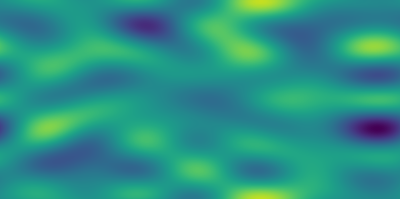
\includegraphics[interpolate=false,width=1.000000in,height=1.000000in]{burgers_rollout_target_0.1-img0.png}}%
\end{pgfscope}%
\begin{pgfscope}%
\pgfsetbuttcap%
\pgfsetroundjoin%
\definecolor{currentfill}{rgb}{0.000000,0.000000,0.000000}%
\pgfsetfillcolor{currentfill}%
\pgfsetlinewidth{0.803000pt}%
\definecolor{currentstroke}{rgb}{0.000000,0.000000,0.000000}%
\pgfsetstrokecolor{currentstroke}%
\pgfsetdash{}{0pt}%
\pgfsys@defobject{currentmarker}{\pgfqpoint{0.000000in}{-0.048611in}}{\pgfqpoint{0.000000in}{0.000000in}}{%
\pgfpathmoveto{\pgfqpoint{0.000000in}{0.000000in}}%
\pgfpathlineto{\pgfqpoint{0.000000in}{-0.048611in}}%
\pgfusepath{stroke,fill}%
}%
\begin{pgfscope}%
\pgfsys@transformshift{0.726837in}{0.517039in}%
\pgfsys@useobject{currentmarker}{}%
\end{pgfscope}%
\end{pgfscope}%
\begin{pgfscope}%
\definecolor{textcolor}{rgb}{0.000000,0.000000,0.000000}%
\pgfsetstrokecolor{textcolor}%
\pgfsetfillcolor{textcolor}%
\pgftext[x=0.726837in,y=0.419816in,,top]{\color{textcolor}\rmfamily\fontsize{12.000000}{14.400000}\selectfont 0}%
\end{pgfscope}%
\begin{pgfscope}%
\pgfsetbuttcap%
\pgfsetroundjoin%
\definecolor{currentfill}{rgb}{0.000000,0.000000,0.000000}%
\pgfsetfillcolor{currentfill}%
\pgfsetlinewidth{0.803000pt}%
\definecolor{currentstroke}{rgb}{0.000000,0.000000,0.000000}%
\pgfsetstrokecolor{currentstroke}%
\pgfsetdash{}{0pt}%
\pgfsys@defobject{currentmarker}{\pgfqpoint{0.000000in}{-0.048611in}}{\pgfqpoint{0.000000in}{0.000000in}}{%
\pgfpathmoveto{\pgfqpoint{0.000000in}{0.000000in}}%
\pgfpathlineto{\pgfqpoint{0.000000in}{-0.048611in}}%
\pgfusepath{stroke,fill}%
}%
\begin{pgfscope}%
\pgfsys@transformshift{1.570762in}{0.517039in}%
\pgfsys@useobject{currentmarker}{}%
\end{pgfscope}%
\end{pgfscope}%
\begin{pgfscope}%
\definecolor{textcolor}{rgb}{0.000000,0.000000,0.000000}%
\pgfsetstrokecolor{textcolor}%
\pgfsetfillcolor{textcolor}%
\pgftext[x=1.570762in,y=0.419816in,,top]{\color{textcolor}\rmfamily\fontsize{12.000000}{14.400000}\selectfont 1}%
\end{pgfscope}%
\begin{pgfscope}%
\pgfsetbuttcap%
\pgfsetroundjoin%
\definecolor{currentfill}{rgb}{0.000000,0.000000,0.000000}%
\pgfsetfillcolor{currentfill}%
\pgfsetlinewidth{0.803000pt}%
\definecolor{currentstroke}{rgb}{0.000000,0.000000,0.000000}%
\pgfsetstrokecolor{currentstroke}%
\pgfsetdash{}{0pt}%
\pgfsys@defobject{currentmarker}{\pgfqpoint{0.000000in}{-0.048611in}}{\pgfqpoint{0.000000in}{0.000000in}}{%
\pgfpathmoveto{\pgfqpoint{0.000000in}{0.000000in}}%
\pgfpathlineto{\pgfqpoint{0.000000in}{-0.048611in}}%
\pgfusepath{stroke,fill}%
}%
\begin{pgfscope}%
\pgfsys@transformshift{2.414687in}{0.517039in}%
\pgfsys@useobject{currentmarker}{}%
\end{pgfscope}%
\end{pgfscope}%
\begin{pgfscope}%
\definecolor{textcolor}{rgb}{0.000000,0.000000,0.000000}%
\pgfsetstrokecolor{textcolor}%
\pgfsetfillcolor{textcolor}%
\pgftext[x=2.414687in,y=0.419816in,,top]{\color{textcolor}\rmfamily\fontsize{12.000000}{14.400000}\selectfont 2}%
\end{pgfscope}%
\begin{pgfscope}%
\definecolor{textcolor}{rgb}{0.000000,0.000000,0.000000}%
\pgfsetstrokecolor{textcolor}%
\pgfsetfillcolor{textcolor}%
\pgftext[x=1.570762in,y=0.202965in,,top]{\color{textcolor}\rmfamily\fontsize{12.000000}{14.400000}\selectfont Space}%
\end{pgfscope}%
\begin{pgfscope}%
\pgfsetbuttcap%
\pgfsetroundjoin%
\definecolor{currentfill}{rgb}{0.000000,0.000000,0.000000}%
\pgfsetfillcolor{currentfill}%
\pgfsetlinewidth{0.803000pt}%
\definecolor{currentstroke}{rgb}{0.000000,0.000000,0.000000}%
\pgfsetstrokecolor{currentstroke}%
\pgfsetdash{}{0pt}%
\pgfsys@defobject{currentmarker}{\pgfqpoint{-0.048611in}{0.000000in}}{\pgfqpoint{-0.000000in}{0.000000in}}{%
\pgfpathmoveto{\pgfqpoint{-0.000000in}{0.000000in}}%
\pgfpathlineto{\pgfqpoint{-0.048611in}{0.000000in}}%
\pgfusepath{stroke,fill}%
}%
\begin{pgfscope}%
\pgfsys@transformshift{0.726837in}{0.517039in}%
\pgfsys@useobject{currentmarker}{}%
\end{pgfscope}%
\end{pgfscope}%
\begin{pgfscope}%
\definecolor{textcolor}{rgb}{0.000000,0.000000,0.000000}%
\pgfsetstrokecolor{textcolor}%
\pgfsetfillcolor{textcolor}%
\pgftext[x=0.364559in, y=0.453725in, left, base]{\color{textcolor}\rmfamily\fontsize{12.000000}{14.400000}\selectfont 0.0}%
\end{pgfscope}%
\begin{pgfscope}%
\pgfsetbuttcap%
\pgfsetroundjoin%
\definecolor{currentfill}{rgb}{0.000000,0.000000,0.000000}%
\pgfsetfillcolor{currentfill}%
\pgfsetlinewidth{0.803000pt}%
\definecolor{currentstroke}{rgb}{0.000000,0.000000,0.000000}%
\pgfsetstrokecolor{currentstroke}%
\pgfsetdash{}{0pt}%
\pgfsys@defobject{currentmarker}{\pgfqpoint{-0.048611in}{0.000000in}}{\pgfqpoint{-0.000000in}{0.000000in}}{%
\pgfpathmoveto{\pgfqpoint{-0.000000in}{0.000000in}}%
\pgfpathlineto{\pgfqpoint{-0.048611in}{0.000000in}}%
\pgfusepath{stroke,fill}%
}%
\begin{pgfscope}%
\pgfsys@transformshift{0.726837in}{0.861533in}%
\pgfsys@useobject{currentmarker}{}%
\end{pgfscope}%
\end{pgfscope}%
\begin{pgfscope}%
\definecolor{textcolor}{rgb}{0.000000,0.000000,0.000000}%
\pgfsetstrokecolor{textcolor}%
\pgfsetfillcolor{textcolor}%
\pgftext[x=0.364559in, y=0.798219in, left, base]{\color{textcolor}\rmfamily\fontsize{12.000000}{14.400000}\selectfont 2.5}%
\end{pgfscope}%
\begin{pgfscope}%
\pgfsetbuttcap%
\pgfsetroundjoin%
\definecolor{currentfill}{rgb}{0.000000,0.000000,0.000000}%
\pgfsetfillcolor{currentfill}%
\pgfsetlinewidth{0.803000pt}%
\definecolor{currentstroke}{rgb}{0.000000,0.000000,0.000000}%
\pgfsetstrokecolor{currentstroke}%
\pgfsetdash{}{0pt}%
\pgfsys@defobject{currentmarker}{\pgfqpoint{-0.048611in}{0.000000in}}{\pgfqpoint{-0.000000in}{0.000000in}}{%
\pgfpathmoveto{\pgfqpoint{-0.000000in}{0.000000in}}%
\pgfpathlineto{\pgfqpoint{-0.048611in}{0.000000in}}%
\pgfusepath{stroke,fill}%
}%
\begin{pgfscope}%
\pgfsys@transformshift{0.726837in}{1.206027in}%
\pgfsys@useobject{currentmarker}{}%
\end{pgfscope}%
\end{pgfscope}%
\begin{pgfscope}%
\definecolor{textcolor}{rgb}{0.000000,0.000000,0.000000}%
\pgfsetstrokecolor{textcolor}%
\pgfsetfillcolor{textcolor}%
\pgftext[x=0.364559in, y=1.142714in, left, base]{\color{textcolor}\rmfamily\fontsize{12.000000}{14.400000}\selectfont 5.0}%
\end{pgfscope}%
\begin{pgfscope}%
\pgfsetbuttcap%
\pgfsetroundjoin%
\definecolor{currentfill}{rgb}{0.000000,0.000000,0.000000}%
\pgfsetfillcolor{currentfill}%
\pgfsetlinewidth{0.803000pt}%
\definecolor{currentstroke}{rgb}{0.000000,0.000000,0.000000}%
\pgfsetstrokecolor{currentstroke}%
\pgfsetdash{}{0pt}%
\pgfsys@defobject{currentmarker}{\pgfqpoint{-0.048611in}{0.000000in}}{\pgfqpoint{-0.000000in}{0.000000in}}{%
\pgfpathmoveto{\pgfqpoint{-0.000000in}{0.000000in}}%
\pgfpathlineto{\pgfqpoint{-0.048611in}{0.000000in}}%
\pgfusepath{stroke,fill}%
}%
\begin{pgfscope}%
\pgfsys@transformshift{0.726837in}{1.550522in}%
\pgfsys@useobject{currentmarker}{}%
\end{pgfscope}%
\end{pgfscope}%
\begin{pgfscope}%
\definecolor{textcolor}{rgb}{0.000000,0.000000,0.000000}%
\pgfsetstrokecolor{textcolor}%
\pgfsetfillcolor{textcolor}%
\pgftext[x=0.364559in, y=1.487208in, left, base]{\color{textcolor}\rmfamily\fontsize{12.000000}{14.400000}\selectfont 7.5}%
\end{pgfscope}%
\begin{pgfscope}%
\pgfsetbuttcap%
\pgfsetroundjoin%
\definecolor{currentfill}{rgb}{0.000000,0.000000,0.000000}%
\pgfsetfillcolor{currentfill}%
\pgfsetlinewidth{0.803000pt}%
\definecolor{currentstroke}{rgb}{0.000000,0.000000,0.000000}%
\pgfsetstrokecolor{currentstroke}%
\pgfsetdash{}{0pt}%
\pgfsys@defobject{currentmarker}{\pgfqpoint{-0.048611in}{0.000000in}}{\pgfqpoint{-0.000000in}{0.000000in}}{%
\pgfpathmoveto{\pgfqpoint{-0.000000in}{0.000000in}}%
\pgfpathlineto{\pgfqpoint{-0.048611in}{0.000000in}}%
\pgfusepath{stroke,fill}%
}%
\begin{pgfscope}%
\pgfsys@transformshift{0.726837in}{1.895016in}%
\pgfsys@useobject{currentmarker}{}%
\end{pgfscope}%
\end{pgfscope}%
\begin{pgfscope}%
\definecolor{textcolor}{rgb}{0.000000,0.000000,0.000000}%
\pgfsetstrokecolor{textcolor}%
\pgfsetfillcolor{textcolor}%
\pgftext[x=0.258521in, y=1.831702in, left, base]{\color{textcolor}\rmfamily\fontsize{12.000000}{14.400000}\selectfont 10.0}%
\end{pgfscope}%
\begin{pgfscope}%
\definecolor{textcolor}{rgb}{0.000000,0.000000,0.000000}%
\pgfsetstrokecolor{textcolor}%
\pgfsetfillcolor{textcolor}%
\pgftext[x=0.202965in,y=1.206027in,,bottom,rotate=90.000000]{\color{textcolor}\rmfamily\fontsize{12.000000}{14.400000}\selectfont Time}%
\end{pgfscope}%
\begin{pgfscope}%
\pgfsetrectcap%
\pgfsetmiterjoin%
\pgfsetlinewidth{0.803000pt}%
\definecolor{currentstroke}{rgb}{0.000000,0.000000,0.000000}%
\pgfsetstrokecolor{currentstroke}%
\pgfsetdash{}{0pt}%
\pgfpathmoveto{\pgfqpoint{0.726837in}{0.517039in}}%
\pgfpathlineto{\pgfqpoint{0.726837in}{1.895016in}}%
\pgfusepath{stroke}%
\end{pgfscope}%
\begin{pgfscope}%
\pgfsetrectcap%
\pgfsetmiterjoin%
\pgfsetlinewidth{0.803000pt}%
\definecolor{currentstroke}{rgb}{0.000000,0.000000,0.000000}%
\pgfsetstrokecolor{currentstroke}%
\pgfsetdash{}{0pt}%
\pgfpathmoveto{\pgfqpoint{2.414687in}{0.517039in}}%
\pgfpathlineto{\pgfqpoint{2.414687in}{1.895016in}}%
\pgfusepath{stroke}%
\end{pgfscope}%
\begin{pgfscope}%
\pgfsetrectcap%
\pgfsetmiterjoin%
\pgfsetlinewidth{0.803000pt}%
\definecolor{currentstroke}{rgb}{0.000000,0.000000,0.000000}%
\pgfsetstrokecolor{currentstroke}%
\pgfsetdash{}{0pt}%
\pgfpathmoveto{\pgfqpoint{0.726837in}{0.517039in}}%
\pgfpathlineto{\pgfqpoint{2.414687in}{0.517039in}}%
\pgfusepath{stroke}%
\end{pgfscope}%
\begin{pgfscope}%
\pgfsetrectcap%
\pgfsetmiterjoin%
\pgfsetlinewidth{0.803000pt}%
\definecolor{currentstroke}{rgb}{0.000000,0.000000,0.000000}%
\pgfsetstrokecolor{currentstroke}%
\pgfsetdash{}{0pt}%
\pgfpathmoveto{\pgfqpoint{0.726837in}{1.895016in}}%
\pgfpathlineto{\pgfqpoint{2.414687in}{1.895016in}}%
\pgfusepath{stroke}%
\end{pgfscope}%
\begin{pgfscope}%
\pgfsetbuttcap%
\pgfsetmiterjoin%
\pgfsetlinewidth{0.000000pt}%
\definecolor{currentstroke}{rgb}{0.000000,0.000000,0.000000}%
\pgfsetstrokecolor{currentstroke}%
\pgfsetstrokeopacity{0.000000}%
\pgfsetdash{}{0pt}%
\pgfpathmoveto{\pgfqpoint{2.552099in}{0.517039in}}%
\pgfpathlineto{\pgfqpoint{2.620998in}{0.517039in}}%
\pgfpathlineto{\pgfqpoint{2.620998in}{1.895016in}}%
\pgfpathlineto{\pgfqpoint{2.552099in}{1.895016in}}%
\pgfpathlineto{\pgfqpoint{2.552099in}{0.517039in}}%
\pgfpathclose%
\pgfusepath{}%
\end{pgfscope}%
\begin{pgfscope}%
\pgfsys@transformshift{2.550000in}{0.520000in}%
\pgftext[left,bottom]{
\includegraphics[interpolate=true,width=0.070000in,height=1.380000in]{burgers_rollout_target_0.1-img1.png}}%
\end{pgfscope}%
\begin{pgfscope}%
\pgfsetbuttcap%
\pgfsetroundjoin%
\definecolor{currentfill}{rgb}{0.000000,0.000000,0.000000}%
\pgfsetfillcolor{currentfill}%
\pgfsetlinewidth{0.803000pt}%
\definecolor{currentstroke}{rgb}{0.000000,0.000000,0.000000}%
\pgfsetstrokecolor{currentstroke}%
\pgfsetdash{}{0pt}%
\pgfsys@defobject{currentmarker}{\pgfqpoint{0.000000in}{0.000000in}}{\pgfqpoint{0.048611in}{0.000000in}}{%
\pgfpathmoveto{\pgfqpoint{0.000000in}{0.000000in}}%
\pgfpathlineto{\pgfqpoint{0.048611in}{0.000000in}}%
\pgfusepath{stroke,fill}%
}%
\begin{pgfscope}%
\pgfsys@transformshift{2.620998in}{0.588723in}%
\pgfsys@useobject{currentmarker}{}%
\end{pgfscope}%
\end{pgfscope}%
\begin{pgfscope}%
\definecolor{textcolor}{rgb}{0.000000,0.000000,0.000000}%
\pgfsetstrokecolor{textcolor}%
\pgfsetfillcolor{textcolor}%
\pgftext[x=2.718220in, y=0.525410in, left, base]{\color{textcolor}\rmfamily\fontsize{12.000000}{14.400000}\selectfont \ensuremath{-}1}%
\end{pgfscope}%
\begin{pgfscope}%
\pgfsetbuttcap%
\pgfsetroundjoin%
\definecolor{currentfill}{rgb}{0.000000,0.000000,0.000000}%
\pgfsetfillcolor{currentfill}%
\pgfsetlinewidth{0.803000pt}%
\definecolor{currentstroke}{rgb}{0.000000,0.000000,0.000000}%
\pgfsetstrokecolor{currentstroke}%
\pgfsetdash{}{0pt}%
\pgfsys@defobject{currentmarker}{\pgfqpoint{0.000000in}{0.000000in}}{\pgfqpoint{0.048611in}{0.000000in}}{%
\pgfpathmoveto{\pgfqpoint{0.000000in}{0.000000in}}%
\pgfpathlineto{\pgfqpoint{0.048611in}{0.000000in}}%
\pgfusepath{stroke,fill}%
}%
\begin{pgfscope}%
\pgfsys@transformshift{2.620998in}{1.206027in}%
\pgfsys@useobject{currentmarker}{}%
\end{pgfscope}%
\end{pgfscope}%
\begin{pgfscope}%
\definecolor{textcolor}{rgb}{0.000000,0.000000,0.000000}%
\pgfsetstrokecolor{textcolor}%
\pgfsetfillcolor{textcolor}%
\pgftext[x=2.718220in, y=1.142714in, left, base]{\color{textcolor}\rmfamily\fontsize{12.000000}{14.400000}\selectfont 0}%
\end{pgfscope}%
\begin{pgfscope}%
\pgfsetbuttcap%
\pgfsetroundjoin%
\definecolor{currentfill}{rgb}{0.000000,0.000000,0.000000}%
\pgfsetfillcolor{currentfill}%
\pgfsetlinewidth{0.803000pt}%
\definecolor{currentstroke}{rgb}{0.000000,0.000000,0.000000}%
\pgfsetstrokecolor{currentstroke}%
\pgfsetdash{}{0pt}%
\pgfsys@defobject{currentmarker}{\pgfqpoint{0.000000in}{0.000000in}}{\pgfqpoint{0.048611in}{0.000000in}}{%
\pgfpathmoveto{\pgfqpoint{0.000000in}{0.000000in}}%
\pgfpathlineto{\pgfqpoint{0.048611in}{0.000000in}}%
\pgfusepath{stroke,fill}%
}%
\begin{pgfscope}%
\pgfsys@transformshift{2.620998in}{1.823331in}%
\pgfsys@useobject{currentmarker}{}%
\end{pgfscope}%
\end{pgfscope}%
\begin{pgfscope}%
\definecolor{textcolor}{rgb}{0.000000,0.000000,0.000000}%
\pgfsetstrokecolor{textcolor}%
\pgfsetfillcolor{textcolor}%
\pgftext[x=2.718220in, y=1.760018in, left, base]{\color{textcolor}\rmfamily\fontsize{12.000000}{14.400000}\selectfont 1}%
\end{pgfscope}%
\begin{pgfscope}%
\pgfsetrectcap%
\pgfsetmiterjoin%
\pgfsetlinewidth{0.803000pt}%
\definecolor{currentstroke}{rgb}{0.000000,0.000000,0.000000}%
\pgfsetstrokecolor{currentstroke}%
\pgfsetdash{}{0pt}%
\pgfpathmoveto{\pgfqpoint{2.552099in}{0.517039in}}%
\pgfpathlineto{\pgfqpoint{2.586548in}{0.517039in}}%
\pgfpathlineto{\pgfqpoint{2.620998in}{0.517039in}}%
\pgfpathlineto{\pgfqpoint{2.620998in}{1.895016in}}%
\pgfpathlineto{\pgfqpoint{2.586548in}{1.895016in}}%
\pgfpathlineto{\pgfqpoint{2.552099in}{1.895016in}}%
\pgfpathlineto{\pgfqpoint{2.552099in}{0.517039in}}%
\pgfpathclose%
\pgfusepath{stroke}%
\end{pgfscope}%
\end{pgfpicture}%
\makeatother%
\endgroup%

      \end{adjustbox}
      \caption{The target for \(\nu=0.1\)}\label{fig:sc2_rollout_target_0.1}
    \end{subfigure}
    \begin{subfigure}{0.33\linewidth}
      \begin{adjustbox}{width=\linewidth}
        \begingroup%
\makeatletter%
\begin{pgfpicture}%
\pgfpathrectangle{\pgfpointorigin}{\pgfqpoint{3.000000in}{2.000000in}}%
\pgfusepath{use as bounding box, clip}%
\begin{pgfscope}%
\pgfsetbuttcap%
\pgfsetmiterjoin%
\pgfsetlinewidth{0.000000pt}%
\definecolor{currentstroke}{rgb}{0.000000,0.000000,0.000000}%
\pgfsetstrokecolor{currentstroke}%
\pgfsetstrokeopacity{0.000000}%
\pgfsetdash{}{0pt}%
\pgfpathmoveto{\pgfqpoint{0.000000in}{0.000000in}}%
\pgfpathlineto{\pgfqpoint{3.000000in}{0.000000in}}%
\pgfpathlineto{\pgfqpoint{3.000000in}{2.000000in}}%
\pgfpathlineto{\pgfqpoint{0.000000in}{2.000000in}}%
\pgfpathlineto{\pgfqpoint{0.000000in}{0.000000in}}%
\pgfpathclose%
\pgfusepath{}%
\end{pgfscope}%
\begin{pgfscope}%
\pgfsetbuttcap%
\pgfsetmiterjoin%
\pgfsetlinewidth{0.000000pt}%
\definecolor{currentstroke}{rgb}{0.000000,0.000000,0.000000}%
\pgfsetstrokecolor{currentstroke}%
\pgfsetstrokeopacity{0.000000}%
\pgfsetdash{}{0pt}%
\pgfpathmoveto{\pgfqpoint{0.726837in}{0.517039in}}%
\pgfpathlineto{\pgfqpoint{2.414687in}{0.517039in}}%
\pgfpathlineto{\pgfqpoint{2.414687in}{1.895016in}}%
\pgfpathlineto{\pgfqpoint{0.726837in}{1.895016in}}%
\pgfpathlineto{\pgfqpoint{0.726837in}{0.517039in}}%
\pgfpathclose%
\pgfusepath{}%
\end{pgfscope}%
\begin{pgfscope}%
\pgfpathrectangle{\pgfqpoint{0.726837in}{0.517039in}}{\pgfqpoint{1.687850in}{1.377978in}}%
\pgfusepath{clip}%
\pgfsys@transformcm{1.687850}{0.000000}{0.000000}{1.377978}{0.726837in}{0.517039in}%
\pgftext[left,bottom]{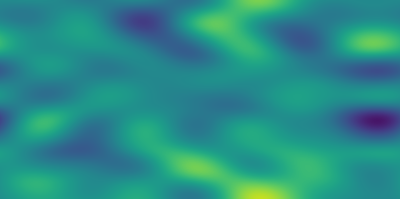
\includegraphics[interpolate=false,width=1.000000in,height=1.000000in]{burgers_rollout_pred_0.1-img0.png}}%
\end{pgfscope}%
\begin{pgfscope}%
\pgfsetbuttcap%
\pgfsetroundjoin%
\definecolor{currentfill}{rgb}{0.000000,0.000000,0.000000}%
\pgfsetfillcolor{currentfill}%
\pgfsetlinewidth{0.803000pt}%
\definecolor{currentstroke}{rgb}{0.000000,0.000000,0.000000}%
\pgfsetstrokecolor{currentstroke}%
\pgfsetdash{}{0pt}%
\pgfsys@defobject{currentmarker}{\pgfqpoint{0.000000in}{-0.048611in}}{\pgfqpoint{0.000000in}{0.000000in}}{%
\pgfpathmoveto{\pgfqpoint{0.000000in}{0.000000in}}%
\pgfpathlineto{\pgfqpoint{0.000000in}{-0.048611in}}%
\pgfusepath{stroke,fill}%
}%
\begin{pgfscope}%
\pgfsys@transformshift{0.726837in}{0.517039in}%
\pgfsys@useobject{currentmarker}{}%
\end{pgfscope}%
\end{pgfscope}%
\begin{pgfscope}%
\definecolor{textcolor}{rgb}{0.000000,0.000000,0.000000}%
\pgfsetstrokecolor{textcolor}%
\pgfsetfillcolor{textcolor}%
\pgftext[x=0.726837in,y=0.419816in,,top]{\color{textcolor}\rmfamily\fontsize{12.000000}{14.400000}\selectfont 0}%
\end{pgfscope}%
\begin{pgfscope}%
\pgfsetbuttcap%
\pgfsetroundjoin%
\definecolor{currentfill}{rgb}{0.000000,0.000000,0.000000}%
\pgfsetfillcolor{currentfill}%
\pgfsetlinewidth{0.803000pt}%
\definecolor{currentstroke}{rgb}{0.000000,0.000000,0.000000}%
\pgfsetstrokecolor{currentstroke}%
\pgfsetdash{}{0pt}%
\pgfsys@defobject{currentmarker}{\pgfqpoint{0.000000in}{-0.048611in}}{\pgfqpoint{0.000000in}{0.000000in}}{%
\pgfpathmoveto{\pgfqpoint{0.000000in}{0.000000in}}%
\pgfpathlineto{\pgfqpoint{0.000000in}{-0.048611in}}%
\pgfusepath{stroke,fill}%
}%
\begin{pgfscope}%
\pgfsys@transformshift{1.570762in}{0.517039in}%
\pgfsys@useobject{currentmarker}{}%
\end{pgfscope}%
\end{pgfscope}%
\begin{pgfscope}%
\definecolor{textcolor}{rgb}{0.000000,0.000000,0.000000}%
\pgfsetstrokecolor{textcolor}%
\pgfsetfillcolor{textcolor}%
\pgftext[x=1.570762in,y=0.419816in,,top]{\color{textcolor}\rmfamily\fontsize{12.000000}{14.400000}\selectfont 1}%
\end{pgfscope}%
\begin{pgfscope}%
\pgfsetbuttcap%
\pgfsetroundjoin%
\definecolor{currentfill}{rgb}{0.000000,0.000000,0.000000}%
\pgfsetfillcolor{currentfill}%
\pgfsetlinewidth{0.803000pt}%
\definecolor{currentstroke}{rgb}{0.000000,0.000000,0.000000}%
\pgfsetstrokecolor{currentstroke}%
\pgfsetdash{}{0pt}%
\pgfsys@defobject{currentmarker}{\pgfqpoint{0.000000in}{-0.048611in}}{\pgfqpoint{0.000000in}{0.000000in}}{%
\pgfpathmoveto{\pgfqpoint{0.000000in}{0.000000in}}%
\pgfpathlineto{\pgfqpoint{0.000000in}{-0.048611in}}%
\pgfusepath{stroke,fill}%
}%
\begin{pgfscope}%
\pgfsys@transformshift{2.414687in}{0.517039in}%
\pgfsys@useobject{currentmarker}{}%
\end{pgfscope}%
\end{pgfscope}%
\begin{pgfscope}%
\definecolor{textcolor}{rgb}{0.000000,0.000000,0.000000}%
\pgfsetstrokecolor{textcolor}%
\pgfsetfillcolor{textcolor}%
\pgftext[x=2.414687in,y=0.419816in,,top]{\color{textcolor}\rmfamily\fontsize{12.000000}{14.400000}\selectfont 2}%
\end{pgfscope}%
\begin{pgfscope}%
\definecolor{textcolor}{rgb}{0.000000,0.000000,0.000000}%
\pgfsetstrokecolor{textcolor}%
\pgfsetfillcolor{textcolor}%
\pgftext[x=1.570762in,y=0.202965in,,top]{\color{textcolor}\rmfamily\fontsize{12.000000}{14.400000}\selectfont Space}%
\end{pgfscope}%
\begin{pgfscope}%
\pgfsetbuttcap%
\pgfsetroundjoin%
\definecolor{currentfill}{rgb}{0.000000,0.000000,0.000000}%
\pgfsetfillcolor{currentfill}%
\pgfsetlinewidth{0.803000pt}%
\definecolor{currentstroke}{rgb}{0.000000,0.000000,0.000000}%
\pgfsetstrokecolor{currentstroke}%
\pgfsetdash{}{0pt}%
\pgfsys@defobject{currentmarker}{\pgfqpoint{-0.048611in}{0.000000in}}{\pgfqpoint{-0.000000in}{0.000000in}}{%
\pgfpathmoveto{\pgfqpoint{-0.000000in}{0.000000in}}%
\pgfpathlineto{\pgfqpoint{-0.048611in}{0.000000in}}%
\pgfusepath{stroke,fill}%
}%
\begin{pgfscope}%
\pgfsys@transformshift{0.726837in}{0.517039in}%
\pgfsys@useobject{currentmarker}{}%
\end{pgfscope}%
\end{pgfscope}%
\begin{pgfscope}%
\definecolor{textcolor}{rgb}{0.000000,0.000000,0.000000}%
\pgfsetstrokecolor{textcolor}%
\pgfsetfillcolor{textcolor}%
\pgftext[x=0.364559in, y=0.453725in, left, base]{\color{textcolor}\rmfamily\fontsize{12.000000}{14.400000}\selectfont 0.0}%
\end{pgfscope}%
\begin{pgfscope}%
\pgfsetbuttcap%
\pgfsetroundjoin%
\definecolor{currentfill}{rgb}{0.000000,0.000000,0.000000}%
\pgfsetfillcolor{currentfill}%
\pgfsetlinewidth{0.803000pt}%
\definecolor{currentstroke}{rgb}{0.000000,0.000000,0.000000}%
\pgfsetstrokecolor{currentstroke}%
\pgfsetdash{}{0pt}%
\pgfsys@defobject{currentmarker}{\pgfqpoint{-0.048611in}{0.000000in}}{\pgfqpoint{-0.000000in}{0.000000in}}{%
\pgfpathmoveto{\pgfqpoint{-0.000000in}{0.000000in}}%
\pgfpathlineto{\pgfqpoint{-0.048611in}{0.000000in}}%
\pgfusepath{stroke,fill}%
}%
\begin{pgfscope}%
\pgfsys@transformshift{0.726837in}{0.861533in}%
\pgfsys@useobject{currentmarker}{}%
\end{pgfscope}%
\end{pgfscope}%
\begin{pgfscope}%
\definecolor{textcolor}{rgb}{0.000000,0.000000,0.000000}%
\pgfsetstrokecolor{textcolor}%
\pgfsetfillcolor{textcolor}%
\pgftext[x=0.364559in, y=0.798219in, left, base]{\color{textcolor}\rmfamily\fontsize{12.000000}{14.400000}\selectfont 2.5}%
\end{pgfscope}%
\begin{pgfscope}%
\pgfsetbuttcap%
\pgfsetroundjoin%
\definecolor{currentfill}{rgb}{0.000000,0.000000,0.000000}%
\pgfsetfillcolor{currentfill}%
\pgfsetlinewidth{0.803000pt}%
\definecolor{currentstroke}{rgb}{0.000000,0.000000,0.000000}%
\pgfsetstrokecolor{currentstroke}%
\pgfsetdash{}{0pt}%
\pgfsys@defobject{currentmarker}{\pgfqpoint{-0.048611in}{0.000000in}}{\pgfqpoint{-0.000000in}{0.000000in}}{%
\pgfpathmoveto{\pgfqpoint{-0.000000in}{0.000000in}}%
\pgfpathlineto{\pgfqpoint{-0.048611in}{0.000000in}}%
\pgfusepath{stroke,fill}%
}%
\begin{pgfscope}%
\pgfsys@transformshift{0.726837in}{1.206027in}%
\pgfsys@useobject{currentmarker}{}%
\end{pgfscope}%
\end{pgfscope}%
\begin{pgfscope}%
\definecolor{textcolor}{rgb}{0.000000,0.000000,0.000000}%
\pgfsetstrokecolor{textcolor}%
\pgfsetfillcolor{textcolor}%
\pgftext[x=0.364559in, y=1.142714in, left, base]{\color{textcolor}\rmfamily\fontsize{12.000000}{14.400000}\selectfont 5.0}%
\end{pgfscope}%
\begin{pgfscope}%
\pgfsetbuttcap%
\pgfsetroundjoin%
\definecolor{currentfill}{rgb}{0.000000,0.000000,0.000000}%
\pgfsetfillcolor{currentfill}%
\pgfsetlinewidth{0.803000pt}%
\definecolor{currentstroke}{rgb}{0.000000,0.000000,0.000000}%
\pgfsetstrokecolor{currentstroke}%
\pgfsetdash{}{0pt}%
\pgfsys@defobject{currentmarker}{\pgfqpoint{-0.048611in}{0.000000in}}{\pgfqpoint{-0.000000in}{0.000000in}}{%
\pgfpathmoveto{\pgfqpoint{-0.000000in}{0.000000in}}%
\pgfpathlineto{\pgfqpoint{-0.048611in}{0.000000in}}%
\pgfusepath{stroke,fill}%
}%
\begin{pgfscope}%
\pgfsys@transformshift{0.726837in}{1.550522in}%
\pgfsys@useobject{currentmarker}{}%
\end{pgfscope}%
\end{pgfscope}%
\begin{pgfscope}%
\definecolor{textcolor}{rgb}{0.000000,0.000000,0.000000}%
\pgfsetstrokecolor{textcolor}%
\pgfsetfillcolor{textcolor}%
\pgftext[x=0.364559in, y=1.487208in, left, base]{\color{textcolor}\rmfamily\fontsize{12.000000}{14.400000}\selectfont 7.5}%
\end{pgfscope}%
\begin{pgfscope}%
\pgfsetbuttcap%
\pgfsetroundjoin%
\definecolor{currentfill}{rgb}{0.000000,0.000000,0.000000}%
\pgfsetfillcolor{currentfill}%
\pgfsetlinewidth{0.803000pt}%
\definecolor{currentstroke}{rgb}{0.000000,0.000000,0.000000}%
\pgfsetstrokecolor{currentstroke}%
\pgfsetdash{}{0pt}%
\pgfsys@defobject{currentmarker}{\pgfqpoint{-0.048611in}{0.000000in}}{\pgfqpoint{-0.000000in}{0.000000in}}{%
\pgfpathmoveto{\pgfqpoint{-0.000000in}{0.000000in}}%
\pgfpathlineto{\pgfqpoint{-0.048611in}{0.000000in}}%
\pgfusepath{stroke,fill}%
}%
\begin{pgfscope}%
\pgfsys@transformshift{0.726837in}{1.895016in}%
\pgfsys@useobject{currentmarker}{}%
\end{pgfscope}%
\end{pgfscope}%
\begin{pgfscope}%
\definecolor{textcolor}{rgb}{0.000000,0.000000,0.000000}%
\pgfsetstrokecolor{textcolor}%
\pgfsetfillcolor{textcolor}%
\pgftext[x=0.258521in, y=1.831702in, left, base]{\color{textcolor}\rmfamily\fontsize{12.000000}{14.400000}\selectfont 10.0}%
\end{pgfscope}%
\begin{pgfscope}%
\definecolor{textcolor}{rgb}{0.000000,0.000000,0.000000}%
\pgfsetstrokecolor{textcolor}%
\pgfsetfillcolor{textcolor}%
\pgftext[x=0.202965in,y=1.206027in,,bottom,rotate=90.000000]{\color{textcolor}\rmfamily\fontsize{12.000000}{14.400000}\selectfont Time}%
\end{pgfscope}%
\begin{pgfscope}%
\pgfsetrectcap%
\pgfsetmiterjoin%
\pgfsetlinewidth{0.803000pt}%
\definecolor{currentstroke}{rgb}{0.000000,0.000000,0.000000}%
\pgfsetstrokecolor{currentstroke}%
\pgfsetdash{}{0pt}%
\pgfpathmoveto{\pgfqpoint{0.726837in}{0.517039in}}%
\pgfpathlineto{\pgfqpoint{0.726837in}{1.895016in}}%
\pgfusepath{stroke}%
\end{pgfscope}%
\begin{pgfscope}%
\pgfsetrectcap%
\pgfsetmiterjoin%
\pgfsetlinewidth{0.803000pt}%
\definecolor{currentstroke}{rgb}{0.000000,0.000000,0.000000}%
\pgfsetstrokecolor{currentstroke}%
\pgfsetdash{}{0pt}%
\pgfpathmoveto{\pgfqpoint{2.414687in}{0.517039in}}%
\pgfpathlineto{\pgfqpoint{2.414687in}{1.895016in}}%
\pgfusepath{stroke}%
\end{pgfscope}%
\begin{pgfscope}%
\pgfsetrectcap%
\pgfsetmiterjoin%
\pgfsetlinewidth{0.803000pt}%
\definecolor{currentstroke}{rgb}{0.000000,0.000000,0.000000}%
\pgfsetstrokecolor{currentstroke}%
\pgfsetdash{}{0pt}%
\pgfpathmoveto{\pgfqpoint{0.726837in}{0.517039in}}%
\pgfpathlineto{\pgfqpoint{2.414687in}{0.517039in}}%
\pgfusepath{stroke}%
\end{pgfscope}%
\begin{pgfscope}%
\pgfsetrectcap%
\pgfsetmiterjoin%
\pgfsetlinewidth{0.803000pt}%
\definecolor{currentstroke}{rgb}{0.000000,0.000000,0.000000}%
\pgfsetstrokecolor{currentstroke}%
\pgfsetdash{}{0pt}%
\pgfpathmoveto{\pgfqpoint{0.726837in}{1.895016in}}%
\pgfpathlineto{\pgfqpoint{2.414687in}{1.895016in}}%
\pgfusepath{stroke}%
\end{pgfscope}%
\begin{pgfscope}%
\pgfsetbuttcap%
\pgfsetmiterjoin%
\pgfsetlinewidth{0.000000pt}%
\definecolor{currentstroke}{rgb}{0.000000,0.000000,0.000000}%
\pgfsetstrokecolor{currentstroke}%
\pgfsetstrokeopacity{0.000000}%
\pgfsetdash{}{0pt}%
\pgfpathmoveto{\pgfqpoint{2.552099in}{0.517039in}}%
\pgfpathlineto{\pgfqpoint{2.620998in}{0.517039in}}%
\pgfpathlineto{\pgfqpoint{2.620998in}{1.895016in}}%
\pgfpathlineto{\pgfqpoint{2.552099in}{1.895016in}}%
\pgfpathlineto{\pgfqpoint{2.552099in}{0.517039in}}%
\pgfpathclose%
\pgfusepath{}%
\end{pgfscope}%
\begin{pgfscope}%
\pgfsys@transformshift{2.550000in}{0.520000in}%
\pgftext[left,bottom]{
\includegraphics[interpolate=true,width=0.070000in,height=1.380000in]{burgers_rollout_pred_0.1-img1.png}}%
\end{pgfscope}%
\begin{pgfscope}%
\pgfsetbuttcap%
\pgfsetroundjoin%
\definecolor{currentfill}{rgb}{0.000000,0.000000,0.000000}%
\pgfsetfillcolor{currentfill}%
\pgfsetlinewidth{0.803000pt}%
\definecolor{currentstroke}{rgb}{0.000000,0.000000,0.000000}%
\pgfsetstrokecolor{currentstroke}%
\pgfsetdash{}{0pt}%
\pgfsys@defobject{currentmarker}{\pgfqpoint{0.000000in}{0.000000in}}{\pgfqpoint{0.048611in}{0.000000in}}{%
\pgfpathmoveto{\pgfqpoint{0.000000in}{0.000000in}}%
\pgfpathlineto{\pgfqpoint{0.048611in}{0.000000in}}%
\pgfusepath{stroke,fill}%
}%
\begin{pgfscope}%
\pgfsys@transformshift{2.620998in}{0.588723in}%
\pgfsys@useobject{currentmarker}{}%
\end{pgfscope}%
\end{pgfscope}%
\begin{pgfscope}%
\definecolor{textcolor}{rgb}{0.000000,0.000000,0.000000}%
\pgfsetstrokecolor{textcolor}%
\pgfsetfillcolor{textcolor}%
\pgftext[x=2.718220in, y=0.525410in, left, base]{\color{textcolor}\rmfamily\fontsize{12.000000}{14.400000}\selectfont \ensuremath{-}1}%
\end{pgfscope}%
\begin{pgfscope}%
\pgfsetbuttcap%
\pgfsetroundjoin%
\definecolor{currentfill}{rgb}{0.000000,0.000000,0.000000}%
\pgfsetfillcolor{currentfill}%
\pgfsetlinewidth{0.803000pt}%
\definecolor{currentstroke}{rgb}{0.000000,0.000000,0.000000}%
\pgfsetstrokecolor{currentstroke}%
\pgfsetdash{}{0pt}%
\pgfsys@defobject{currentmarker}{\pgfqpoint{0.000000in}{0.000000in}}{\pgfqpoint{0.048611in}{0.000000in}}{%
\pgfpathmoveto{\pgfqpoint{0.000000in}{0.000000in}}%
\pgfpathlineto{\pgfqpoint{0.048611in}{0.000000in}}%
\pgfusepath{stroke,fill}%
}%
\begin{pgfscope}%
\pgfsys@transformshift{2.620998in}{1.206027in}%
\pgfsys@useobject{currentmarker}{}%
\end{pgfscope}%
\end{pgfscope}%
\begin{pgfscope}%
\definecolor{textcolor}{rgb}{0.000000,0.000000,0.000000}%
\pgfsetstrokecolor{textcolor}%
\pgfsetfillcolor{textcolor}%
\pgftext[x=2.718220in, y=1.142714in, left, base]{\color{textcolor}\rmfamily\fontsize{12.000000}{14.400000}\selectfont 0}%
\end{pgfscope}%
\begin{pgfscope}%
\pgfsetbuttcap%
\pgfsetroundjoin%
\definecolor{currentfill}{rgb}{0.000000,0.000000,0.000000}%
\pgfsetfillcolor{currentfill}%
\pgfsetlinewidth{0.803000pt}%
\definecolor{currentstroke}{rgb}{0.000000,0.000000,0.000000}%
\pgfsetstrokecolor{currentstroke}%
\pgfsetdash{}{0pt}%
\pgfsys@defobject{currentmarker}{\pgfqpoint{0.000000in}{0.000000in}}{\pgfqpoint{0.048611in}{0.000000in}}{%
\pgfpathmoveto{\pgfqpoint{0.000000in}{0.000000in}}%
\pgfpathlineto{\pgfqpoint{0.048611in}{0.000000in}}%
\pgfusepath{stroke,fill}%
}%
\begin{pgfscope}%
\pgfsys@transformshift{2.620998in}{1.823331in}%
\pgfsys@useobject{currentmarker}{}%
\end{pgfscope}%
\end{pgfscope}%
\begin{pgfscope}%
\definecolor{textcolor}{rgb}{0.000000,0.000000,0.000000}%
\pgfsetstrokecolor{textcolor}%
\pgfsetfillcolor{textcolor}%
\pgftext[x=2.718220in, y=1.760018in, left, base]{\color{textcolor}\rmfamily\fontsize{12.000000}{14.400000}\selectfont 1}%
\end{pgfscope}%
\begin{pgfscope}%
\pgfsetrectcap%
\pgfsetmiterjoin%
\pgfsetlinewidth{0.803000pt}%
\definecolor{currentstroke}{rgb}{0.000000,0.000000,0.000000}%
\pgfsetstrokecolor{currentstroke}%
\pgfsetdash{}{0pt}%
\pgfpathmoveto{\pgfqpoint{2.552099in}{0.517039in}}%
\pgfpathlineto{\pgfqpoint{2.586548in}{0.517039in}}%
\pgfpathlineto{\pgfqpoint{2.620998in}{0.517039in}}%
\pgfpathlineto{\pgfqpoint{2.620998in}{1.895016in}}%
\pgfpathlineto{\pgfqpoint{2.586548in}{1.895016in}}%
\pgfpathlineto{\pgfqpoint{2.552099in}{1.895016in}}%
\pgfpathlineto{\pgfqpoint{2.552099in}{0.517039in}}%
\pgfpathclose%
\pgfusepath{stroke}%
\end{pgfscope}%
\end{pgfpicture}%
\makeatother%
\endgroup%

      \end{adjustbox}
      \caption{The prediction for \(\nu=0.1\)}\label{fig:sc2_rollout_pred_0.1}
    \end{subfigure}
    \begin{subfigure}{0.32\linewidth}
      \begin{adjustbox}{width=\linewidth}
        \begingroup%
\makeatletter%
\begin{pgfpicture}%
\pgfpathrectangle{\pgfpointorigin}{\pgfqpoint{3.000000in}{2.000000in}}%
\pgfusepath{use as bounding box, clip}%
\begin{pgfscope}%
\pgfsetbuttcap%
\pgfsetmiterjoin%
\pgfsetlinewidth{0.000000pt}%
\definecolor{currentstroke}{rgb}{0.000000,0.000000,0.000000}%
\pgfsetstrokecolor{currentstroke}%
\pgfsetstrokeopacity{0.000000}%
\pgfsetdash{}{0pt}%
\pgfpathmoveto{\pgfqpoint{0.000000in}{0.000000in}}%
\pgfpathlineto{\pgfqpoint{3.000000in}{0.000000in}}%
\pgfpathlineto{\pgfqpoint{3.000000in}{2.000000in}}%
\pgfpathlineto{\pgfqpoint{0.000000in}{2.000000in}}%
\pgfpathlineto{\pgfqpoint{0.000000in}{0.000000in}}%
\pgfpathclose%
\pgfusepath{}%
\end{pgfscope}%
\begin{pgfscope}%
\pgfsetbuttcap%
\pgfsetmiterjoin%
\pgfsetlinewidth{0.000000pt}%
\definecolor{currentstroke}{rgb}{0.000000,0.000000,0.000000}%
\pgfsetstrokecolor{currentstroke}%
\pgfsetstrokeopacity{0.000000}%
\pgfsetdash{}{0pt}%
\pgfpathmoveto{\pgfqpoint{0.726837in}{0.517039in}}%
\pgfpathlineto{\pgfqpoint{2.414687in}{0.517039in}}%
\pgfpathlineto{\pgfqpoint{2.414687in}{1.895016in}}%
\pgfpathlineto{\pgfqpoint{0.726837in}{1.895016in}}%
\pgfpathlineto{\pgfqpoint{0.726837in}{0.517039in}}%
\pgfpathclose%
\pgfusepath{}%
\end{pgfscope}%
\begin{pgfscope}%
\pgfpathrectangle{\pgfqpoint{0.726837in}{0.517039in}}{\pgfqpoint{1.687850in}{1.377978in}}%
\pgfusepath{clip}%
\pgfsys@transformcm{1.687850}{0.000000}{0.000000}{1.377978}{0.726837in}{0.517039in}%
\pgftext[left,bottom]{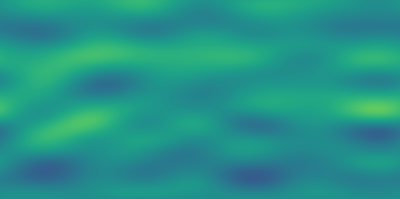
\includegraphics[interpolate=false,width=1.000000in,height=1.000000in]{burgers_rollout_diff_0.1-img0.png}}%
\end{pgfscope}%
\begin{pgfscope}%
\pgfsetbuttcap%
\pgfsetroundjoin%
\definecolor{currentfill}{rgb}{0.000000,0.000000,0.000000}%
\pgfsetfillcolor{currentfill}%
\pgfsetlinewidth{0.803000pt}%
\definecolor{currentstroke}{rgb}{0.000000,0.000000,0.000000}%
\pgfsetstrokecolor{currentstroke}%
\pgfsetdash{}{0pt}%
\pgfsys@defobject{currentmarker}{\pgfqpoint{0.000000in}{-0.048611in}}{\pgfqpoint{0.000000in}{0.000000in}}{%
\pgfpathmoveto{\pgfqpoint{0.000000in}{0.000000in}}%
\pgfpathlineto{\pgfqpoint{0.000000in}{-0.048611in}}%
\pgfusepath{stroke,fill}%
}%
\begin{pgfscope}%
\pgfsys@transformshift{0.726837in}{0.517039in}%
\pgfsys@useobject{currentmarker}{}%
\end{pgfscope}%
\end{pgfscope}%
\begin{pgfscope}%
\definecolor{textcolor}{rgb}{0.000000,0.000000,0.000000}%
\pgfsetstrokecolor{textcolor}%
\pgfsetfillcolor{textcolor}%
\pgftext[x=0.726837in,y=0.419816in,,top]{\color{textcolor}\rmfamily\fontsize{12.000000}{14.400000}\selectfont 0}%
\end{pgfscope}%
\begin{pgfscope}%
\pgfsetbuttcap%
\pgfsetroundjoin%
\definecolor{currentfill}{rgb}{0.000000,0.000000,0.000000}%
\pgfsetfillcolor{currentfill}%
\pgfsetlinewidth{0.803000pt}%
\definecolor{currentstroke}{rgb}{0.000000,0.000000,0.000000}%
\pgfsetstrokecolor{currentstroke}%
\pgfsetdash{}{0pt}%
\pgfsys@defobject{currentmarker}{\pgfqpoint{0.000000in}{-0.048611in}}{\pgfqpoint{0.000000in}{0.000000in}}{%
\pgfpathmoveto{\pgfqpoint{0.000000in}{0.000000in}}%
\pgfpathlineto{\pgfqpoint{0.000000in}{-0.048611in}}%
\pgfusepath{stroke,fill}%
}%
\begin{pgfscope}%
\pgfsys@transformshift{1.570762in}{0.517039in}%
\pgfsys@useobject{currentmarker}{}%
\end{pgfscope}%
\end{pgfscope}%
\begin{pgfscope}%
\definecolor{textcolor}{rgb}{0.000000,0.000000,0.000000}%
\pgfsetstrokecolor{textcolor}%
\pgfsetfillcolor{textcolor}%
\pgftext[x=1.570762in,y=0.419816in,,top]{\color{textcolor}\rmfamily\fontsize{12.000000}{14.400000}\selectfont 1}%
\end{pgfscope}%
\begin{pgfscope}%
\pgfsetbuttcap%
\pgfsetroundjoin%
\definecolor{currentfill}{rgb}{0.000000,0.000000,0.000000}%
\pgfsetfillcolor{currentfill}%
\pgfsetlinewidth{0.803000pt}%
\definecolor{currentstroke}{rgb}{0.000000,0.000000,0.000000}%
\pgfsetstrokecolor{currentstroke}%
\pgfsetdash{}{0pt}%
\pgfsys@defobject{currentmarker}{\pgfqpoint{0.000000in}{-0.048611in}}{\pgfqpoint{0.000000in}{0.000000in}}{%
\pgfpathmoveto{\pgfqpoint{0.000000in}{0.000000in}}%
\pgfpathlineto{\pgfqpoint{0.000000in}{-0.048611in}}%
\pgfusepath{stroke,fill}%
}%
\begin{pgfscope}%
\pgfsys@transformshift{2.414687in}{0.517039in}%
\pgfsys@useobject{currentmarker}{}%
\end{pgfscope}%
\end{pgfscope}%
\begin{pgfscope}%
\definecolor{textcolor}{rgb}{0.000000,0.000000,0.000000}%
\pgfsetstrokecolor{textcolor}%
\pgfsetfillcolor{textcolor}%
\pgftext[x=2.414687in,y=0.419816in,,top]{\color{textcolor}\rmfamily\fontsize{12.000000}{14.400000}\selectfont 2}%
\end{pgfscope}%
\begin{pgfscope}%
\definecolor{textcolor}{rgb}{0.000000,0.000000,0.000000}%
\pgfsetstrokecolor{textcolor}%
\pgfsetfillcolor{textcolor}%
\pgftext[x=1.570762in,y=0.202965in,,top]{\color{textcolor}\rmfamily\fontsize{12.000000}{14.400000}\selectfont Space}%
\end{pgfscope}%
\begin{pgfscope}%
\pgfsetbuttcap%
\pgfsetroundjoin%
\definecolor{currentfill}{rgb}{0.000000,0.000000,0.000000}%
\pgfsetfillcolor{currentfill}%
\pgfsetlinewidth{0.803000pt}%
\definecolor{currentstroke}{rgb}{0.000000,0.000000,0.000000}%
\pgfsetstrokecolor{currentstroke}%
\pgfsetdash{}{0pt}%
\pgfsys@defobject{currentmarker}{\pgfqpoint{-0.048611in}{0.000000in}}{\pgfqpoint{-0.000000in}{0.000000in}}{%
\pgfpathmoveto{\pgfqpoint{-0.000000in}{0.000000in}}%
\pgfpathlineto{\pgfqpoint{-0.048611in}{0.000000in}}%
\pgfusepath{stroke,fill}%
}%
\begin{pgfscope}%
\pgfsys@transformshift{0.726837in}{0.517039in}%
\pgfsys@useobject{currentmarker}{}%
\end{pgfscope}%
\end{pgfscope}%
\begin{pgfscope}%
\definecolor{textcolor}{rgb}{0.000000,0.000000,0.000000}%
\pgfsetstrokecolor{textcolor}%
\pgfsetfillcolor{textcolor}%
\pgftext[x=0.364559in, y=0.453725in, left, base]{\color{textcolor}\rmfamily\fontsize{12.000000}{14.400000}\selectfont 0.0}%
\end{pgfscope}%
\begin{pgfscope}%
\pgfsetbuttcap%
\pgfsetroundjoin%
\definecolor{currentfill}{rgb}{0.000000,0.000000,0.000000}%
\pgfsetfillcolor{currentfill}%
\pgfsetlinewidth{0.803000pt}%
\definecolor{currentstroke}{rgb}{0.000000,0.000000,0.000000}%
\pgfsetstrokecolor{currentstroke}%
\pgfsetdash{}{0pt}%
\pgfsys@defobject{currentmarker}{\pgfqpoint{-0.048611in}{0.000000in}}{\pgfqpoint{-0.000000in}{0.000000in}}{%
\pgfpathmoveto{\pgfqpoint{-0.000000in}{0.000000in}}%
\pgfpathlineto{\pgfqpoint{-0.048611in}{0.000000in}}%
\pgfusepath{stroke,fill}%
}%
\begin{pgfscope}%
\pgfsys@transformshift{0.726837in}{0.861533in}%
\pgfsys@useobject{currentmarker}{}%
\end{pgfscope}%
\end{pgfscope}%
\begin{pgfscope}%
\definecolor{textcolor}{rgb}{0.000000,0.000000,0.000000}%
\pgfsetstrokecolor{textcolor}%
\pgfsetfillcolor{textcolor}%
\pgftext[x=0.364559in, y=0.798219in, left, base]{\color{textcolor}\rmfamily\fontsize{12.000000}{14.400000}\selectfont 2.5}%
\end{pgfscope}%
\begin{pgfscope}%
\pgfsetbuttcap%
\pgfsetroundjoin%
\definecolor{currentfill}{rgb}{0.000000,0.000000,0.000000}%
\pgfsetfillcolor{currentfill}%
\pgfsetlinewidth{0.803000pt}%
\definecolor{currentstroke}{rgb}{0.000000,0.000000,0.000000}%
\pgfsetstrokecolor{currentstroke}%
\pgfsetdash{}{0pt}%
\pgfsys@defobject{currentmarker}{\pgfqpoint{-0.048611in}{0.000000in}}{\pgfqpoint{-0.000000in}{0.000000in}}{%
\pgfpathmoveto{\pgfqpoint{-0.000000in}{0.000000in}}%
\pgfpathlineto{\pgfqpoint{-0.048611in}{0.000000in}}%
\pgfusepath{stroke,fill}%
}%
\begin{pgfscope}%
\pgfsys@transformshift{0.726837in}{1.206027in}%
\pgfsys@useobject{currentmarker}{}%
\end{pgfscope}%
\end{pgfscope}%
\begin{pgfscope}%
\definecolor{textcolor}{rgb}{0.000000,0.000000,0.000000}%
\pgfsetstrokecolor{textcolor}%
\pgfsetfillcolor{textcolor}%
\pgftext[x=0.364559in, y=1.142714in, left, base]{\color{textcolor}\rmfamily\fontsize{12.000000}{14.400000}\selectfont 5.0}%
\end{pgfscope}%
\begin{pgfscope}%
\pgfsetbuttcap%
\pgfsetroundjoin%
\definecolor{currentfill}{rgb}{0.000000,0.000000,0.000000}%
\pgfsetfillcolor{currentfill}%
\pgfsetlinewidth{0.803000pt}%
\definecolor{currentstroke}{rgb}{0.000000,0.000000,0.000000}%
\pgfsetstrokecolor{currentstroke}%
\pgfsetdash{}{0pt}%
\pgfsys@defobject{currentmarker}{\pgfqpoint{-0.048611in}{0.000000in}}{\pgfqpoint{-0.000000in}{0.000000in}}{%
\pgfpathmoveto{\pgfqpoint{-0.000000in}{0.000000in}}%
\pgfpathlineto{\pgfqpoint{-0.048611in}{0.000000in}}%
\pgfusepath{stroke,fill}%
}%
\begin{pgfscope}%
\pgfsys@transformshift{0.726837in}{1.550522in}%
\pgfsys@useobject{currentmarker}{}%
\end{pgfscope}%
\end{pgfscope}%
\begin{pgfscope}%
\definecolor{textcolor}{rgb}{0.000000,0.000000,0.000000}%
\pgfsetstrokecolor{textcolor}%
\pgfsetfillcolor{textcolor}%
\pgftext[x=0.364559in, y=1.487208in, left, base]{\color{textcolor}\rmfamily\fontsize{12.000000}{14.400000}\selectfont 7.5}%
\end{pgfscope}%
\begin{pgfscope}%
\pgfsetbuttcap%
\pgfsetroundjoin%
\definecolor{currentfill}{rgb}{0.000000,0.000000,0.000000}%
\pgfsetfillcolor{currentfill}%
\pgfsetlinewidth{0.803000pt}%
\definecolor{currentstroke}{rgb}{0.000000,0.000000,0.000000}%
\pgfsetstrokecolor{currentstroke}%
\pgfsetdash{}{0pt}%
\pgfsys@defobject{currentmarker}{\pgfqpoint{-0.048611in}{0.000000in}}{\pgfqpoint{-0.000000in}{0.000000in}}{%
\pgfpathmoveto{\pgfqpoint{-0.000000in}{0.000000in}}%
\pgfpathlineto{\pgfqpoint{-0.048611in}{0.000000in}}%
\pgfusepath{stroke,fill}%
}%
\begin{pgfscope}%
\pgfsys@transformshift{0.726837in}{1.895016in}%
\pgfsys@useobject{currentmarker}{}%
\end{pgfscope}%
\end{pgfscope}%
\begin{pgfscope}%
\definecolor{textcolor}{rgb}{0.000000,0.000000,0.000000}%
\pgfsetstrokecolor{textcolor}%
\pgfsetfillcolor{textcolor}%
\pgftext[x=0.258521in, y=1.831702in, left, base]{\color{textcolor}\rmfamily\fontsize{12.000000}{14.400000}\selectfont 10.0}%
\end{pgfscope}%
\begin{pgfscope}%
\definecolor{textcolor}{rgb}{0.000000,0.000000,0.000000}%
\pgfsetstrokecolor{textcolor}%
\pgfsetfillcolor{textcolor}%
\pgftext[x=0.202965in,y=1.206027in,,bottom,rotate=90.000000]{\color{textcolor}\rmfamily\fontsize{12.000000}{14.400000}\selectfont Time}%
\end{pgfscope}%
\begin{pgfscope}%
\pgfsetrectcap%
\pgfsetmiterjoin%
\pgfsetlinewidth{0.803000pt}%
\definecolor{currentstroke}{rgb}{0.000000,0.000000,0.000000}%
\pgfsetstrokecolor{currentstroke}%
\pgfsetdash{}{0pt}%
\pgfpathmoveto{\pgfqpoint{0.726837in}{0.517039in}}%
\pgfpathlineto{\pgfqpoint{0.726837in}{1.895016in}}%
\pgfusepath{stroke}%
\end{pgfscope}%
\begin{pgfscope}%
\pgfsetrectcap%
\pgfsetmiterjoin%
\pgfsetlinewidth{0.803000pt}%
\definecolor{currentstroke}{rgb}{0.000000,0.000000,0.000000}%
\pgfsetstrokecolor{currentstroke}%
\pgfsetdash{}{0pt}%
\pgfpathmoveto{\pgfqpoint{2.414687in}{0.517039in}}%
\pgfpathlineto{\pgfqpoint{2.414687in}{1.895016in}}%
\pgfusepath{stroke}%
\end{pgfscope}%
\begin{pgfscope}%
\pgfsetrectcap%
\pgfsetmiterjoin%
\pgfsetlinewidth{0.803000pt}%
\definecolor{currentstroke}{rgb}{0.000000,0.000000,0.000000}%
\pgfsetstrokecolor{currentstroke}%
\pgfsetdash{}{0pt}%
\pgfpathmoveto{\pgfqpoint{0.726837in}{0.517039in}}%
\pgfpathlineto{\pgfqpoint{2.414687in}{0.517039in}}%
\pgfusepath{stroke}%
\end{pgfscope}%
\begin{pgfscope}%
\pgfsetrectcap%
\pgfsetmiterjoin%
\pgfsetlinewidth{0.803000pt}%
\definecolor{currentstroke}{rgb}{0.000000,0.000000,0.000000}%
\pgfsetstrokecolor{currentstroke}%
\pgfsetdash{}{0pt}%
\pgfpathmoveto{\pgfqpoint{0.726837in}{1.895016in}}%
\pgfpathlineto{\pgfqpoint{2.414687in}{1.895016in}}%
\pgfusepath{stroke}%
\end{pgfscope}%
\begin{pgfscope}%
\pgfsetbuttcap%
\pgfsetmiterjoin%
\pgfsetlinewidth{0.000000pt}%
\definecolor{currentstroke}{rgb}{0.000000,0.000000,0.000000}%
\pgfsetstrokecolor{currentstroke}%
\pgfsetstrokeopacity{0.000000}%
\pgfsetdash{}{0pt}%
\pgfpathmoveto{\pgfqpoint{2.552099in}{0.517039in}}%
\pgfpathlineto{\pgfqpoint{2.620998in}{0.517039in}}%
\pgfpathlineto{\pgfqpoint{2.620998in}{1.895016in}}%
\pgfpathlineto{\pgfqpoint{2.552099in}{1.895016in}}%
\pgfpathlineto{\pgfqpoint{2.552099in}{0.517039in}}%
\pgfpathclose%
\pgfusepath{}%
\end{pgfscope}%
\begin{pgfscope}%
\pgfsys@transformshift{2.550000in}{0.520000in}%
\pgftext[left,bottom]{
\includegraphics[interpolate=true,width=0.070000in,height=1.380000in]{burgers_rollout_diff_0.1-img1.png}}%
\end{pgfscope}%
\begin{pgfscope}%
\pgfsetbuttcap%
\pgfsetroundjoin%
\definecolor{currentfill}{rgb}{0.000000,0.000000,0.000000}%
\pgfsetfillcolor{currentfill}%
\pgfsetlinewidth{0.803000pt}%
\definecolor{currentstroke}{rgb}{0.000000,0.000000,0.000000}%
\pgfsetstrokecolor{currentstroke}%
\pgfsetdash{}{0pt}%
\pgfsys@defobject{currentmarker}{\pgfqpoint{0.000000in}{0.000000in}}{\pgfqpoint{0.048611in}{0.000000in}}{%
\pgfpathmoveto{\pgfqpoint{0.000000in}{0.000000in}}%
\pgfpathlineto{\pgfqpoint{0.048611in}{0.000000in}}%
\pgfusepath{stroke,fill}%
}%
\begin{pgfscope}%
\pgfsys@transformshift{2.620998in}{0.588723in}%
\pgfsys@useobject{currentmarker}{}%
\end{pgfscope}%
\end{pgfscope}%
\begin{pgfscope}%
\definecolor{textcolor}{rgb}{0.000000,0.000000,0.000000}%
\pgfsetstrokecolor{textcolor}%
\pgfsetfillcolor{textcolor}%
\pgftext[x=2.718220in, y=0.525410in, left, base]{\color{textcolor}\rmfamily\fontsize{12.000000}{14.400000}\selectfont \ensuremath{-}1}%
\end{pgfscope}%
\begin{pgfscope}%
\pgfsetbuttcap%
\pgfsetroundjoin%
\definecolor{currentfill}{rgb}{0.000000,0.000000,0.000000}%
\pgfsetfillcolor{currentfill}%
\pgfsetlinewidth{0.803000pt}%
\definecolor{currentstroke}{rgb}{0.000000,0.000000,0.000000}%
\pgfsetstrokecolor{currentstroke}%
\pgfsetdash{}{0pt}%
\pgfsys@defobject{currentmarker}{\pgfqpoint{0.000000in}{0.000000in}}{\pgfqpoint{0.048611in}{0.000000in}}{%
\pgfpathmoveto{\pgfqpoint{0.000000in}{0.000000in}}%
\pgfpathlineto{\pgfqpoint{0.048611in}{0.000000in}}%
\pgfusepath{stroke,fill}%
}%
\begin{pgfscope}%
\pgfsys@transformshift{2.620998in}{1.206027in}%
\pgfsys@useobject{currentmarker}{}%
\end{pgfscope}%
\end{pgfscope}%
\begin{pgfscope}%
\definecolor{textcolor}{rgb}{0.000000,0.000000,0.000000}%
\pgfsetstrokecolor{textcolor}%
\pgfsetfillcolor{textcolor}%
\pgftext[x=2.718220in, y=1.142714in, left, base]{\color{textcolor}\rmfamily\fontsize{12.000000}{14.400000}\selectfont 0}%
\end{pgfscope}%
\begin{pgfscope}%
\pgfsetbuttcap%
\pgfsetroundjoin%
\definecolor{currentfill}{rgb}{0.000000,0.000000,0.000000}%
\pgfsetfillcolor{currentfill}%
\pgfsetlinewidth{0.803000pt}%
\definecolor{currentstroke}{rgb}{0.000000,0.000000,0.000000}%
\pgfsetstrokecolor{currentstroke}%
\pgfsetdash{}{0pt}%
\pgfsys@defobject{currentmarker}{\pgfqpoint{0.000000in}{0.000000in}}{\pgfqpoint{0.048611in}{0.000000in}}{%
\pgfpathmoveto{\pgfqpoint{0.000000in}{0.000000in}}%
\pgfpathlineto{\pgfqpoint{0.048611in}{0.000000in}}%
\pgfusepath{stroke,fill}%
}%
\begin{pgfscope}%
\pgfsys@transformshift{2.620998in}{1.823331in}%
\pgfsys@useobject{currentmarker}{}%
\end{pgfscope}%
\end{pgfscope}%
\begin{pgfscope}%
\definecolor{textcolor}{rgb}{0.000000,0.000000,0.000000}%
\pgfsetstrokecolor{textcolor}%
\pgfsetfillcolor{textcolor}%
\pgftext[x=2.718220in, y=1.760018in, left, base]{\color{textcolor}\rmfamily\fontsize{12.000000}{14.400000}\selectfont 1}%
\end{pgfscope}%
\begin{pgfscope}%
\pgfsetrectcap%
\pgfsetmiterjoin%
\pgfsetlinewidth{0.803000pt}%
\definecolor{currentstroke}{rgb}{0.000000,0.000000,0.000000}%
\pgfsetstrokecolor{currentstroke}%
\pgfsetdash{}{0pt}%
\pgfpathmoveto{\pgfqpoint{2.552099in}{0.517039in}}%
\pgfpathlineto{\pgfqpoint{2.586548in}{0.517039in}}%
\pgfpathlineto{\pgfqpoint{2.620998in}{0.517039in}}%
\pgfpathlineto{\pgfqpoint{2.620998in}{1.895016in}}%
\pgfpathlineto{\pgfqpoint{2.586548in}{1.895016in}}%
\pgfpathlineto{\pgfqpoint{2.552099in}{1.895016in}}%
\pgfpathlineto{\pgfqpoint{2.552099in}{0.517039in}}%
\pgfpathclose%
\pgfusepath{stroke}%
\end{pgfscope}%
\end{pgfpicture}%
\makeatother%
\endgroup%

      \end{adjustbox}
      \caption{The difference for \(\nu=0.1\)}\label{fig:sc2_rollout_diff_0.1}
    \end{subfigure}
    % \\[0.7\baselineskip]
  \end{adjustwidth}
  \caption{The rollout predictions for one of the test function. The difference is calculated as the targets subtracted by the predictions.}\label{fig:scenario_2_rollout}
\end{figure}

Another observation we can see is that the difference between the target and rollout predictions is much more pronounced for lower viscosity values. This result is aligned with metrics shown in \lccrefs{table:scenario_2_rollout_function_metrics}. The absolute metrics show that the models are performing several times worse in rollout compared to the single time step tests shown in \lccrefs{table:scenario_2_function_metrics}. This seems to be the same challenge that traditional solvers also face with the shocks that may be present with lower viscosity values. This means that for rollout scenarios, the model has a much harder time with lower viscosity values. The observation here is that for higher viscosity values, the error is dominated by the global error, and the lower viscosity value, the error is dominated by local errors and as such accumulates.
\begin{table}[H]
  \caption{Performance metrics of function values evaluated from coefficient rollout in scenario 2 by viscosity.}\label{table:scenario_2_rollout_function_metrics}
  \centering
  \begin{tabular}{lrrrr}
    \toprule
    \(\nu \) & MSE      & RMSE     & MAE      & sMAPE \\
    \midrule
    0.0      & 5.81e-02 & 2.41e-01 & 1.89e-01 & 1.04  \\
    0.01     & 3.17e-02 & 1.78e-01 & 1.40e-01 & 0.94  \\
    0.1      & 2.91e-02 & 1.71e-01 & 1.33e-01 & 0.92  \\
    \bottomrule
  \end{tabular}
\end{table}

To test the generalization capability of the model on other function families, we use an exact solution provided in the literature shown in \lccref{eq:burgers_exact_solution} \citep{woodExactSolutionBurgers2006,wazwazPartialDifferentialEquations2010,bentonTableSolutionsOnedimensional1972}.
\begin{equation}
  u(x,t) = \frac{2\nu\pi e^{-\pi^2\nu t}\sin(\pi x)}{a+e^{-\pi^2\nu t}\cos(\pi x)} \label{eq:burgers_exact_solution}
\end{equation}

The exact function \cref{eq:burgers_exact_solution} is computed for each viscosity value. The discrete Fourier transform of the values are then used for doing rollout with the model. For the forcing term, we just use a constant function with a value of zero. The rollout predictions are shown in \lccref{fig:scenario_2_exact}. The model is not successful in the rollout for the inviscid equation and for the viscosity of \(\nu=0.01\). Both of these cases, the model produces too much error that the original function is no longer recognizable in the predictions. For the higher viscosity value of \(\nu=0.1\) the rollout produces a recognizable prediction. The error stays to about half the maximum function value. We do see some more noticeable error in the flatter parts of the function. The error also take a very similar shape across the different viscosity values. Since we essentially used the same solutions for training the model for each viscosity, the similarity in error means that it can be alleviated with more diverse training samples. The error for the flatter functions may also be alleviated by including similar flatter functions during training.
\begin{figure}[H]
  \centering
  \begin{adjustwidth}{-0.1\linewidth}{-0.1\linewidth}
    \begin{subfigure}{0.33\linewidth}
      \begin{adjustbox}{width=\linewidth}
        \begingroup%
\makeatletter%
\begin{pgfpicture}%
\pgfpathrectangle{\pgfpointorigin}{\pgfqpoint{3.000000in}{2.000000in}}%
\pgfusepath{use as bounding box, clip}%
\begin{pgfscope}%
\pgfsetbuttcap%
\pgfsetmiterjoin%
\pgfsetlinewidth{0.000000pt}%
\definecolor{currentstroke}{rgb}{0.000000,0.000000,0.000000}%
\pgfsetstrokecolor{currentstroke}%
\pgfsetstrokeopacity{0.000000}%
\pgfsetdash{}{0pt}%
\pgfpathmoveto{\pgfqpoint{0.000000in}{0.000000in}}%
\pgfpathlineto{\pgfqpoint{3.000000in}{0.000000in}}%
\pgfpathlineto{\pgfqpoint{3.000000in}{2.000000in}}%
\pgfpathlineto{\pgfqpoint{0.000000in}{2.000000in}}%
\pgfpathlineto{\pgfqpoint{0.000000in}{0.000000in}}%
\pgfpathclose%
\pgfusepath{}%
\end{pgfscope}%
\begin{pgfscope}%
\pgfsetbuttcap%
\pgfsetmiterjoin%
\pgfsetlinewidth{0.000000pt}%
\definecolor{currentstroke}{rgb}{0.000000,0.000000,0.000000}%
\pgfsetstrokecolor{currentstroke}%
\pgfsetstrokeopacity{0.000000}%
\pgfsetdash{}{0pt}%
\pgfpathmoveto{\pgfqpoint{0.726837in}{0.517039in}}%
\pgfpathlineto{\pgfqpoint{2.263621in}{0.517039in}}%
\pgfpathlineto{\pgfqpoint{2.263621in}{1.895016in}}%
\pgfpathlineto{\pgfqpoint{0.726837in}{1.895016in}}%
\pgfpathlineto{\pgfqpoint{0.726837in}{0.517039in}}%
\pgfpathclose%
\pgfusepath{}%
\end{pgfscope}%
\begin{pgfscope}%
\pgfpathrectangle{\pgfqpoint{0.726837in}{0.517039in}}{\pgfqpoint{1.536784in}{1.377978in}}%
\pgfusepath{clip}%
\pgfsys@transformcm{1.536784}{0.000000}{0.000000}{1.377978}{0.726837in}{0.517039in}%
\pgftext[left,bottom]{
\includegraphics[interpolate=false,width=1.000000in,height=1.000000in]{burgers_exact_target_0.0-img0.png}}%
\end{pgfscope}%
\begin{pgfscope}%
\pgfsetbuttcap%
\pgfsetroundjoin%
\definecolor{currentfill}{rgb}{0.000000,0.000000,0.000000}%
\pgfsetfillcolor{currentfill}%
\pgfsetlinewidth{0.803000pt}%
\definecolor{currentstroke}{rgb}{0.000000,0.000000,0.000000}%
\pgfsetstrokecolor{currentstroke}%
\pgfsetdash{}{0pt}%
\pgfsys@defobject{currentmarker}{\pgfqpoint{0.000000in}{-0.048611in}}{\pgfqpoint{0.000000in}{0.000000in}}{%
\pgfpathmoveto{\pgfqpoint{0.000000in}{0.000000in}}%
\pgfpathlineto{\pgfqpoint{0.000000in}{-0.048611in}}%
\pgfusepath{stroke,fill}%
}%
\begin{pgfscope}%
\pgfsys@transformshift{0.726837in}{0.517039in}%
\pgfsys@useobject{currentmarker}{}%
\end{pgfscope}%
\end{pgfscope}%
\begin{pgfscope}%
\definecolor{textcolor}{rgb}{0.000000,0.000000,0.000000}%
\pgfsetstrokecolor{textcolor}%
\pgfsetfillcolor{textcolor}%
\pgftext[x=0.726837in,y=0.419816in,,top]{\color{textcolor}\rmfamily\fontsize{12.000000}{14.400000}\selectfont 0}%
\end{pgfscope}%
\begin{pgfscope}%
\pgfsetbuttcap%
\pgfsetroundjoin%
\definecolor{currentfill}{rgb}{0.000000,0.000000,0.000000}%
\pgfsetfillcolor{currentfill}%
\pgfsetlinewidth{0.803000pt}%
\definecolor{currentstroke}{rgb}{0.000000,0.000000,0.000000}%
\pgfsetstrokecolor{currentstroke}%
\pgfsetdash{}{0pt}%
\pgfsys@defobject{currentmarker}{\pgfqpoint{0.000000in}{-0.048611in}}{\pgfqpoint{0.000000in}{0.000000in}}{%
\pgfpathmoveto{\pgfqpoint{0.000000in}{0.000000in}}%
\pgfpathlineto{\pgfqpoint{0.000000in}{-0.048611in}}%
\pgfusepath{stroke,fill}%
}%
\begin{pgfscope}%
\pgfsys@transformshift{1.495229in}{0.517039in}%
\pgfsys@useobject{currentmarker}{}%
\end{pgfscope}%
\end{pgfscope}%
\begin{pgfscope}%
\definecolor{textcolor}{rgb}{0.000000,0.000000,0.000000}%
\pgfsetstrokecolor{textcolor}%
\pgfsetfillcolor{textcolor}%
\pgftext[x=1.495229in,y=0.419816in,,top]{\color{textcolor}\rmfamily\fontsize{12.000000}{14.400000}\selectfont 1}%
\end{pgfscope}%
\begin{pgfscope}%
\pgfsetbuttcap%
\pgfsetroundjoin%
\definecolor{currentfill}{rgb}{0.000000,0.000000,0.000000}%
\pgfsetfillcolor{currentfill}%
\pgfsetlinewidth{0.803000pt}%
\definecolor{currentstroke}{rgb}{0.000000,0.000000,0.000000}%
\pgfsetstrokecolor{currentstroke}%
\pgfsetdash{}{0pt}%
\pgfsys@defobject{currentmarker}{\pgfqpoint{0.000000in}{-0.048611in}}{\pgfqpoint{0.000000in}{0.000000in}}{%
\pgfpathmoveto{\pgfqpoint{0.000000in}{0.000000in}}%
\pgfpathlineto{\pgfqpoint{0.000000in}{-0.048611in}}%
\pgfusepath{stroke,fill}%
}%
\begin{pgfscope}%
\pgfsys@transformshift{2.263621in}{0.517039in}%
\pgfsys@useobject{currentmarker}{}%
\end{pgfscope}%
\end{pgfscope}%
\begin{pgfscope}%
\definecolor{textcolor}{rgb}{0.000000,0.000000,0.000000}%
\pgfsetstrokecolor{textcolor}%
\pgfsetfillcolor{textcolor}%
\pgftext[x=2.263621in,y=0.419816in,,top]{\color{textcolor}\rmfamily\fontsize{12.000000}{14.400000}\selectfont 2}%
\end{pgfscope}%
\begin{pgfscope}%
\definecolor{textcolor}{rgb}{0.000000,0.000000,0.000000}%
\pgfsetstrokecolor{textcolor}%
\pgfsetfillcolor{textcolor}%
\pgftext[x=1.495229in,y=0.202965in,,top]{\color{textcolor}\rmfamily\fontsize{12.000000}{14.400000}\selectfont Space}%
\end{pgfscope}%
\begin{pgfscope}%
\pgfsetbuttcap%
\pgfsetroundjoin%
\definecolor{currentfill}{rgb}{0.000000,0.000000,0.000000}%
\pgfsetfillcolor{currentfill}%
\pgfsetlinewidth{0.803000pt}%
\definecolor{currentstroke}{rgb}{0.000000,0.000000,0.000000}%
\pgfsetstrokecolor{currentstroke}%
\pgfsetdash{}{0pt}%
\pgfsys@defobject{currentmarker}{\pgfqpoint{-0.048611in}{0.000000in}}{\pgfqpoint{-0.000000in}{0.000000in}}{%
\pgfpathmoveto{\pgfqpoint{-0.000000in}{0.000000in}}%
\pgfpathlineto{\pgfqpoint{-0.048611in}{0.000000in}}%
\pgfusepath{stroke,fill}%
}%
\begin{pgfscope}%
\pgfsys@transformshift{0.726837in}{0.517039in}%
\pgfsys@useobject{currentmarker}{}%
\end{pgfscope}%
\end{pgfscope}%
\begin{pgfscope}%
\definecolor{textcolor}{rgb}{0.000000,0.000000,0.000000}%
\pgfsetstrokecolor{textcolor}%
\pgfsetfillcolor{textcolor}%
\pgftext[x=0.364559in, y=0.453725in, left, base]{\color{textcolor}\rmfamily\fontsize{12.000000}{14.400000}\selectfont 0.0}%
\end{pgfscope}%
\begin{pgfscope}%
\pgfsetbuttcap%
\pgfsetroundjoin%
\definecolor{currentfill}{rgb}{0.000000,0.000000,0.000000}%
\pgfsetfillcolor{currentfill}%
\pgfsetlinewidth{0.803000pt}%
\definecolor{currentstroke}{rgb}{0.000000,0.000000,0.000000}%
\pgfsetstrokecolor{currentstroke}%
\pgfsetdash{}{0pt}%
\pgfsys@defobject{currentmarker}{\pgfqpoint{-0.048611in}{0.000000in}}{\pgfqpoint{-0.000000in}{0.000000in}}{%
\pgfpathmoveto{\pgfqpoint{-0.000000in}{0.000000in}}%
\pgfpathlineto{\pgfqpoint{-0.048611in}{0.000000in}}%
\pgfusepath{stroke,fill}%
}%
\begin{pgfscope}%
\pgfsys@transformshift{0.726837in}{0.861533in}%
\pgfsys@useobject{currentmarker}{}%
\end{pgfscope}%
\end{pgfscope}%
\begin{pgfscope}%
\definecolor{textcolor}{rgb}{0.000000,0.000000,0.000000}%
\pgfsetstrokecolor{textcolor}%
\pgfsetfillcolor{textcolor}%
\pgftext[x=0.364559in, y=0.798219in, left, base]{\color{textcolor}\rmfamily\fontsize{12.000000}{14.400000}\selectfont 2.5}%
\end{pgfscope}%
\begin{pgfscope}%
\pgfsetbuttcap%
\pgfsetroundjoin%
\definecolor{currentfill}{rgb}{0.000000,0.000000,0.000000}%
\pgfsetfillcolor{currentfill}%
\pgfsetlinewidth{0.803000pt}%
\definecolor{currentstroke}{rgb}{0.000000,0.000000,0.000000}%
\pgfsetstrokecolor{currentstroke}%
\pgfsetdash{}{0pt}%
\pgfsys@defobject{currentmarker}{\pgfqpoint{-0.048611in}{0.000000in}}{\pgfqpoint{-0.000000in}{0.000000in}}{%
\pgfpathmoveto{\pgfqpoint{-0.000000in}{0.000000in}}%
\pgfpathlineto{\pgfqpoint{-0.048611in}{0.000000in}}%
\pgfusepath{stroke,fill}%
}%
\begin{pgfscope}%
\pgfsys@transformshift{0.726837in}{1.206027in}%
\pgfsys@useobject{currentmarker}{}%
\end{pgfscope}%
\end{pgfscope}%
\begin{pgfscope}%
\definecolor{textcolor}{rgb}{0.000000,0.000000,0.000000}%
\pgfsetstrokecolor{textcolor}%
\pgfsetfillcolor{textcolor}%
\pgftext[x=0.364559in, y=1.142714in, left, base]{\color{textcolor}\rmfamily\fontsize{12.000000}{14.400000}\selectfont 5.0}%
\end{pgfscope}%
\begin{pgfscope}%
\pgfsetbuttcap%
\pgfsetroundjoin%
\definecolor{currentfill}{rgb}{0.000000,0.000000,0.000000}%
\pgfsetfillcolor{currentfill}%
\pgfsetlinewidth{0.803000pt}%
\definecolor{currentstroke}{rgb}{0.000000,0.000000,0.000000}%
\pgfsetstrokecolor{currentstroke}%
\pgfsetdash{}{0pt}%
\pgfsys@defobject{currentmarker}{\pgfqpoint{-0.048611in}{0.000000in}}{\pgfqpoint{-0.000000in}{0.000000in}}{%
\pgfpathmoveto{\pgfqpoint{-0.000000in}{0.000000in}}%
\pgfpathlineto{\pgfqpoint{-0.048611in}{0.000000in}}%
\pgfusepath{stroke,fill}%
}%
\begin{pgfscope}%
\pgfsys@transformshift{0.726837in}{1.550522in}%
\pgfsys@useobject{currentmarker}{}%
\end{pgfscope}%
\end{pgfscope}%
\begin{pgfscope}%
\definecolor{textcolor}{rgb}{0.000000,0.000000,0.000000}%
\pgfsetstrokecolor{textcolor}%
\pgfsetfillcolor{textcolor}%
\pgftext[x=0.364559in, y=1.487208in, left, base]{\color{textcolor}\rmfamily\fontsize{12.000000}{14.400000}\selectfont 7.5}%
\end{pgfscope}%
\begin{pgfscope}%
\pgfsetbuttcap%
\pgfsetroundjoin%
\definecolor{currentfill}{rgb}{0.000000,0.000000,0.000000}%
\pgfsetfillcolor{currentfill}%
\pgfsetlinewidth{0.803000pt}%
\definecolor{currentstroke}{rgb}{0.000000,0.000000,0.000000}%
\pgfsetstrokecolor{currentstroke}%
\pgfsetdash{}{0pt}%
\pgfsys@defobject{currentmarker}{\pgfqpoint{-0.048611in}{0.000000in}}{\pgfqpoint{-0.000000in}{0.000000in}}{%
\pgfpathmoveto{\pgfqpoint{-0.000000in}{0.000000in}}%
\pgfpathlineto{\pgfqpoint{-0.048611in}{0.000000in}}%
\pgfusepath{stroke,fill}%
}%
\begin{pgfscope}%
\pgfsys@transformshift{0.726837in}{1.895016in}%
\pgfsys@useobject{currentmarker}{}%
\end{pgfscope}%
\end{pgfscope}%
\begin{pgfscope}%
\definecolor{textcolor}{rgb}{0.000000,0.000000,0.000000}%
\pgfsetstrokecolor{textcolor}%
\pgfsetfillcolor{textcolor}%
\pgftext[x=0.258521in, y=1.831702in, left, base]{\color{textcolor}\rmfamily\fontsize{12.000000}{14.400000}\selectfont 10.0}%
\end{pgfscope}%
\begin{pgfscope}%
\definecolor{textcolor}{rgb}{0.000000,0.000000,0.000000}%
\pgfsetstrokecolor{textcolor}%
\pgfsetfillcolor{textcolor}%
\pgftext[x=0.202965in,y=1.206027in,,bottom,rotate=90.000000]{\color{textcolor}\rmfamily\fontsize{12.000000}{14.400000}\selectfont Time}%
\end{pgfscope}%
\begin{pgfscope}%
\pgfsetrectcap%
\pgfsetmiterjoin%
\pgfsetlinewidth{0.803000pt}%
\definecolor{currentstroke}{rgb}{0.000000,0.000000,0.000000}%
\pgfsetstrokecolor{currentstroke}%
\pgfsetdash{}{0pt}%
\pgfpathmoveto{\pgfqpoint{0.726837in}{0.517039in}}%
\pgfpathlineto{\pgfqpoint{0.726837in}{1.895016in}}%
\pgfusepath{stroke}%
\end{pgfscope}%
\begin{pgfscope}%
\pgfsetrectcap%
\pgfsetmiterjoin%
\pgfsetlinewidth{0.803000pt}%
\definecolor{currentstroke}{rgb}{0.000000,0.000000,0.000000}%
\pgfsetstrokecolor{currentstroke}%
\pgfsetdash{}{0pt}%
\pgfpathmoveto{\pgfqpoint{2.263621in}{0.517039in}}%
\pgfpathlineto{\pgfqpoint{2.263621in}{1.895016in}}%
\pgfusepath{stroke}%
\end{pgfscope}%
\begin{pgfscope}%
\pgfsetrectcap%
\pgfsetmiterjoin%
\pgfsetlinewidth{0.803000pt}%
\definecolor{currentstroke}{rgb}{0.000000,0.000000,0.000000}%
\pgfsetstrokecolor{currentstroke}%
\pgfsetdash{}{0pt}%
\pgfpathmoveto{\pgfqpoint{0.726837in}{0.517039in}}%
\pgfpathlineto{\pgfqpoint{2.263621in}{0.517039in}}%
\pgfusepath{stroke}%
\end{pgfscope}%
\begin{pgfscope}%
\pgfsetrectcap%
\pgfsetmiterjoin%
\pgfsetlinewidth{0.803000pt}%
\definecolor{currentstroke}{rgb}{0.000000,0.000000,0.000000}%
\pgfsetstrokecolor{currentstroke}%
\pgfsetdash{}{0pt}%
\pgfpathmoveto{\pgfqpoint{0.726837in}{1.895016in}}%
\pgfpathlineto{\pgfqpoint{2.263621in}{1.895016in}}%
\pgfusepath{stroke}%
\end{pgfscope}%
\begin{pgfscope}%
\pgfsetbuttcap%
\pgfsetmiterjoin%
\pgfsetlinewidth{0.000000pt}%
\definecolor{currentstroke}{rgb}{0.000000,0.000000,0.000000}%
\pgfsetstrokecolor{currentstroke}%
\pgfsetstrokeopacity{0.000000}%
\pgfsetdash{}{0pt}%
\pgfpathmoveto{\pgfqpoint{2.393479in}{0.517039in}}%
\pgfpathlineto{\pgfqpoint{2.462378in}{0.517039in}}%
\pgfpathlineto{\pgfqpoint{2.462378in}{1.895016in}}%
\pgfpathlineto{\pgfqpoint{2.393479in}{1.895016in}}%
\pgfpathlineto{\pgfqpoint{2.393479in}{0.517039in}}%
\pgfpathclose%
\pgfusepath{}%
\end{pgfscope}%
\begin{pgfscope}%
\pgfsys@transformshift{2.390000in}{0.520000in}%
\pgftext[left,bottom]{
\includegraphics[interpolate=true,width=0.070000in,height=1.380000in]{burgers_exact_target_0.0-img1.png}}%
\end{pgfscope}%
\begin{pgfscope}%
\pgfsetbuttcap%
\pgfsetroundjoin%
\definecolor{currentfill}{rgb}{0.000000,0.000000,0.000000}%
\pgfsetfillcolor{currentfill}%
\pgfsetlinewidth{0.803000pt}%
\definecolor{currentstroke}{rgb}{0.000000,0.000000,0.000000}%
\pgfsetstrokecolor{currentstroke}%
\pgfsetdash{}{0pt}%
\pgfsys@defobject{currentmarker}{\pgfqpoint{0.000000in}{0.000000in}}{\pgfqpoint{0.048611in}{0.000000in}}{%
\pgfpathmoveto{\pgfqpoint{0.000000in}{0.000000in}}%
\pgfpathlineto{\pgfqpoint{0.048611in}{0.000000in}}%
\pgfusepath{stroke,fill}%
}%
\begin{pgfscope}%
\pgfsys@transformshift{2.462378in}{0.565953in}%
\pgfsys@useobject{currentmarker}{}%
\end{pgfscope}%
\end{pgfscope}%
\begin{pgfscope}%
\definecolor{textcolor}{rgb}{0.000000,0.000000,0.000000}%
\pgfsetstrokecolor{textcolor}%
\pgfsetfillcolor{textcolor}%
\pgftext[x=2.559601in, y=0.502639in, left, base]{\color{textcolor}\rmfamily\fontsize{12.000000}{14.400000}\selectfont \ensuremath{-}0.2}%
\end{pgfscope}%
\begin{pgfscope}%
\pgfsetbuttcap%
\pgfsetroundjoin%
\definecolor{currentfill}{rgb}{0.000000,0.000000,0.000000}%
\pgfsetfillcolor{currentfill}%
\pgfsetlinewidth{0.803000pt}%
\definecolor{currentstroke}{rgb}{0.000000,0.000000,0.000000}%
\pgfsetstrokecolor{currentstroke}%
\pgfsetdash{}{0pt}%
\pgfsys@defobject{currentmarker}{\pgfqpoint{0.000000in}{0.000000in}}{\pgfqpoint{0.048611in}{0.000000in}}{%
\pgfpathmoveto{\pgfqpoint{0.000000in}{0.000000in}}%
\pgfpathlineto{\pgfqpoint{0.048611in}{0.000000in}}%
\pgfusepath{stroke,fill}%
}%
\begin{pgfscope}%
\pgfsys@transformshift{2.462378in}{1.206027in}%
\pgfsys@useobject{currentmarker}{}%
\end{pgfscope}%
\end{pgfscope}%
\begin{pgfscope}%
\definecolor{textcolor}{rgb}{0.000000,0.000000,0.000000}%
\pgfsetstrokecolor{textcolor}%
\pgfsetfillcolor{textcolor}%
\pgftext[x=2.559601in, y=1.142714in, left, base]{\color{textcolor}\rmfamily\fontsize{12.000000}{14.400000}\selectfont 0.0}%
\end{pgfscope}%
\begin{pgfscope}%
\pgfsetbuttcap%
\pgfsetroundjoin%
\definecolor{currentfill}{rgb}{0.000000,0.000000,0.000000}%
\pgfsetfillcolor{currentfill}%
\pgfsetlinewidth{0.803000pt}%
\definecolor{currentstroke}{rgb}{0.000000,0.000000,0.000000}%
\pgfsetstrokecolor{currentstroke}%
\pgfsetdash{}{0pt}%
\pgfsys@defobject{currentmarker}{\pgfqpoint{0.000000in}{0.000000in}}{\pgfqpoint{0.048611in}{0.000000in}}{%
\pgfpathmoveto{\pgfqpoint{0.000000in}{0.000000in}}%
\pgfpathlineto{\pgfqpoint{0.048611in}{0.000000in}}%
\pgfusepath{stroke,fill}%
}%
\begin{pgfscope}%
\pgfsys@transformshift{2.462378in}{1.846102in}%
\pgfsys@useobject{currentmarker}{}%
\end{pgfscope}%
\end{pgfscope}%
\begin{pgfscope}%
\definecolor{textcolor}{rgb}{0.000000,0.000000,0.000000}%
\pgfsetstrokecolor{textcolor}%
\pgfsetfillcolor{textcolor}%
\pgftext[x=2.559601in, y=1.782788in, left, base]{\color{textcolor}\rmfamily\fontsize{12.000000}{14.400000}\selectfont 0.2}%
\end{pgfscope}%
\begin{pgfscope}%
\pgfsetrectcap%
\pgfsetmiterjoin%
\pgfsetlinewidth{0.803000pt}%
\definecolor{currentstroke}{rgb}{0.000000,0.000000,0.000000}%
\pgfsetstrokecolor{currentstroke}%
\pgfsetdash{}{0pt}%
\pgfpathmoveto{\pgfqpoint{2.393479in}{0.517039in}}%
\pgfpathlineto{\pgfqpoint{2.427929in}{0.517039in}}%
\pgfpathlineto{\pgfqpoint{2.462378in}{0.517039in}}%
\pgfpathlineto{\pgfqpoint{2.462378in}{1.895016in}}%
\pgfpathlineto{\pgfqpoint{2.427929in}{1.895016in}}%
\pgfpathlineto{\pgfqpoint{2.393479in}{1.895016in}}%
\pgfpathlineto{\pgfqpoint{2.393479in}{0.517039in}}%
\pgfpathclose%
\pgfusepath{stroke}%
\end{pgfscope}%
\end{pgfpicture}%
\makeatother%
\endgroup%

      \end{adjustbox}
      \caption{The target for \(\nu=0.0\)}\label{fig:sc2_exact_target_0.0}
    \end{subfigure}
    \begin{subfigure}{0.33\linewidth}
      \begin{adjustbox}{width=\linewidth}
        \begingroup%
\makeatletter%
\begin{pgfpicture}%
\pgfpathrectangle{\pgfpointorigin}{\pgfqpoint{3.000000in}{2.000000in}}%
\pgfusepath{use as bounding box, clip}%
\begin{pgfscope}%
\pgfsetbuttcap%
\pgfsetmiterjoin%
\pgfsetlinewidth{0.000000pt}%
\definecolor{currentstroke}{rgb}{0.000000,0.000000,0.000000}%
\pgfsetstrokecolor{currentstroke}%
\pgfsetstrokeopacity{0.000000}%
\pgfsetdash{}{0pt}%
\pgfpathmoveto{\pgfqpoint{0.000000in}{0.000000in}}%
\pgfpathlineto{\pgfqpoint{3.000000in}{0.000000in}}%
\pgfpathlineto{\pgfqpoint{3.000000in}{2.000000in}}%
\pgfpathlineto{\pgfqpoint{0.000000in}{2.000000in}}%
\pgfpathlineto{\pgfqpoint{0.000000in}{0.000000in}}%
\pgfpathclose%
\pgfusepath{}%
\end{pgfscope}%
\begin{pgfscope}%
\pgfsetbuttcap%
\pgfsetmiterjoin%
\pgfsetlinewidth{0.000000pt}%
\definecolor{currentstroke}{rgb}{0.000000,0.000000,0.000000}%
\pgfsetstrokecolor{currentstroke}%
\pgfsetstrokeopacity{0.000000}%
\pgfsetdash{}{0pt}%
\pgfpathmoveto{\pgfqpoint{0.726837in}{0.517039in}}%
\pgfpathlineto{\pgfqpoint{2.263621in}{0.517039in}}%
\pgfpathlineto{\pgfqpoint{2.263621in}{1.895016in}}%
\pgfpathlineto{\pgfqpoint{0.726837in}{1.895016in}}%
\pgfpathlineto{\pgfqpoint{0.726837in}{0.517039in}}%
\pgfpathclose%
\pgfusepath{}%
\end{pgfscope}%
\begin{pgfscope}%
\pgfpathrectangle{\pgfqpoint{0.726837in}{0.517039in}}{\pgfqpoint{1.536784in}{1.377978in}}%
\pgfusepath{clip}%
\pgfsys@transformcm{1.536784}{0.000000}{0.000000}{1.377978}{0.726837in}{0.517039in}%
\pgftext[left,bottom]{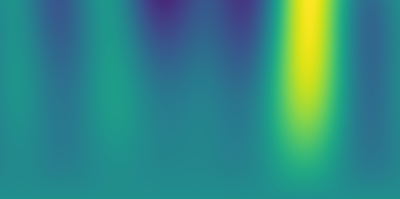
\includegraphics[interpolate=false,width=1.000000in,height=1.000000in]{burgers_exact_pred_0.0-img0.png}}%
\end{pgfscope}%
\begin{pgfscope}%
\pgfsetbuttcap%
\pgfsetroundjoin%
\definecolor{currentfill}{rgb}{0.000000,0.000000,0.000000}%
\pgfsetfillcolor{currentfill}%
\pgfsetlinewidth{0.803000pt}%
\definecolor{currentstroke}{rgb}{0.000000,0.000000,0.000000}%
\pgfsetstrokecolor{currentstroke}%
\pgfsetdash{}{0pt}%
\pgfsys@defobject{currentmarker}{\pgfqpoint{0.000000in}{-0.048611in}}{\pgfqpoint{0.000000in}{0.000000in}}{%
\pgfpathmoveto{\pgfqpoint{0.000000in}{0.000000in}}%
\pgfpathlineto{\pgfqpoint{0.000000in}{-0.048611in}}%
\pgfusepath{stroke,fill}%
}%
\begin{pgfscope}%
\pgfsys@transformshift{0.726837in}{0.517039in}%
\pgfsys@useobject{currentmarker}{}%
\end{pgfscope}%
\end{pgfscope}%
\begin{pgfscope}%
\definecolor{textcolor}{rgb}{0.000000,0.000000,0.000000}%
\pgfsetstrokecolor{textcolor}%
\pgfsetfillcolor{textcolor}%
\pgftext[x=0.726837in,y=0.419816in,,top]{\color{textcolor}{\rmfamily\fontsize{12.000000}{14.400000}\selectfont\catcode`\^=\active\def^{\ifmmode\sp\else\^{}\fi}\catcode`\%=\active\def%{\%}0}}%
\end{pgfscope}%
\begin{pgfscope}%
\pgfsetbuttcap%
\pgfsetroundjoin%
\definecolor{currentfill}{rgb}{0.000000,0.000000,0.000000}%
\pgfsetfillcolor{currentfill}%
\pgfsetlinewidth{0.803000pt}%
\definecolor{currentstroke}{rgb}{0.000000,0.000000,0.000000}%
\pgfsetstrokecolor{currentstroke}%
\pgfsetdash{}{0pt}%
\pgfsys@defobject{currentmarker}{\pgfqpoint{0.000000in}{-0.048611in}}{\pgfqpoint{0.000000in}{0.000000in}}{%
\pgfpathmoveto{\pgfqpoint{0.000000in}{0.000000in}}%
\pgfpathlineto{\pgfqpoint{0.000000in}{-0.048611in}}%
\pgfusepath{stroke,fill}%
}%
\begin{pgfscope}%
\pgfsys@transformshift{1.495229in}{0.517039in}%
\pgfsys@useobject{currentmarker}{}%
\end{pgfscope}%
\end{pgfscope}%
\begin{pgfscope}%
\definecolor{textcolor}{rgb}{0.000000,0.000000,0.000000}%
\pgfsetstrokecolor{textcolor}%
\pgfsetfillcolor{textcolor}%
\pgftext[x=1.495229in,y=0.419816in,,top]{\color{textcolor}{\rmfamily\fontsize{12.000000}{14.400000}\selectfont\catcode`\^=\active\def^{\ifmmode\sp\else\^{}\fi}\catcode`\%=\active\def%{\%}1}}%
\end{pgfscope}%
\begin{pgfscope}%
\pgfsetbuttcap%
\pgfsetroundjoin%
\definecolor{currentfill}{rgb}{0.000000,0.000000,0.000000}%
\pgfsetfillcolor{currentfill}%
\pgfsetlinewidth{0.803000pt}%
\definecolor{currentstroke}{rgb}{0.000000,0.000000,0.000000}%
\pgfsetstrokecolor{currentstroke}%
\pgfsetdash{}{0pt}%
\pgfsys@defobject{currentmarker}{\pgfqpoint{0.000000in}{-0.048611in}}{\pgfqpoint{0.000000in}{0.000000in}}{%
\pgfpathmoveto{\pgfqpoint{0.000000in}{0.000000in}}%
\pgfpathlineto{\pgfqpoint{0.000000in}{-0.048611in}}%
\pgfusepath{stroke,fill}%
}%
\begin{pgfscope}%
\pgfsys@transformshift{2.263621in}{0.517039in}%
\pgfsys@useobject{currentmarker}{}%
\end{pgfscope}%
\end{pgfscope}%
\begin{pgfscope}%
\definecolor{textcolor}{rgb}{0.000000,0.000000,0.000000}%
\pgfsetstrokecolor{textcolor}%
\pgfsetfillcolor{textcolor}%
\pgftext[x=2.263621in,y=0.419816in,,top]{\color{textcolor}{\rmfamily\fontsize{12.000000}{14.400000}\selectfont\catcode`\^=\active\def^{\ifmmode\sp\else\^{}\fi}\catcode`\%=\active\def%{\%}2}}%
\end{pgfscope}%
\begin{pgfscope}%
\definecolor{textcolor}{rgb}{0.000000,0.000000,0.000000}%
\pgfsetstrokecolor{textcolor}%
\pgfsetfillcolor{textcolor}%
\pgftext[x=1.495229in,y=0.202965in,,top]{\color{textcolor}{\rmfamily\fontsize{12.000000}{14.400000}\selectfont\catcode`\^=\active\def^{\ifmmode\sp\else\^{}\fi}\catcode`\%=\active\def%{\%}Space}}%
\end{pgfscope}%
\begin{pgfscope}%
\pgfsetbuttcap%
\pgfsetroundjoin%
\definecolor{currentfill}{rgb}{0.000000,0.000000,0.000000}%
\pgfsetfillcolor{currentfill}%
\pgfsetlinewidth{0.803000pt}%
\definecolor{currentstroke}{rgb}{0.000000,0.000000,0.000000}%
\pgfsetstrokecolor{currentstroke}%
\pgfsetdash{}{0pt}%
\pgfsys@defobject{currentmarker}{\pgfqpoint{-0.048611in}{0.000000in}}{\pgfqpoint{-0.000000in}{0.000000in}}{%
\pgfpathmoveto{\pgfqpoint{-0.000000in}{0.000000in}}%
\pgfpathlineto{\pgfqpoint{-0.048611in}{0.000000in}}%
\pgfusepath{stroke,fill}%
}%
\begin{pgfscope}%
\pgfsys@transformshift{0.726837in}{0.517039in}%
\pgfsys@useobject{currentmarker}{}%
\end{pgfscope}%
\end{pgfscope}%
\begin{pgfscope}%
\definecolor{textcolor}{rgb}{0.000000,0.000000,0.000000}%
\pgfsetstrokecolor{textcolor}%
\pgfsetfillcolor{textcolor}%
\pgftext[x=0.364559in, y=0.453725in, left, base]{\color{textcolor}{\rmfamily\fontsize{12.000000}{14.400000}\selectfont\catcode`\^=\active\def^{\ifmmode\sp\else\^{}\fi}\catcode`\%=\active\def%{\%}0.0}}%
\end{pgfscope}%
\begin{pgfscope}%
\pgfsetbuttcap%
\pgfsetroundjoin%
\definecolor{currentfill}{rgb}{0.000000,0.000000,0.000000}%
\pgfsetfillcolor{currentfill}%
\pgfsetlinewidth{0.803000pt}%
\definecolor{currentstroke}{rgb}{0.000000,0.000000,0.000000}%
\pgfsetstrokecolor{currentstroke}%
\pgfsetdash{}{0pt}%
\pgfsys@defobject{currentmarker}{\pgfqpoint{-0.048611in}{0.000000in}}{\pgfqpoint{-0.000000in}{0.000000in}}{%
\pgfpathmoveto{\pgfqpoint{-0.000000in}{0.000000in}}%
\pgfpathlineto{\pgfqpoint{-0.048611in}{0.000000in}}%
\pgfusepath{stroke,fill}%
}%
\begin{pgfscope}%
\pgfsys@transformshift{0.726837in}{0.861533in}%
\pgfsys@useobject{currentmarker}{}%
\end{pgfscope}%
\end{pgfscope}%
\begin{pgfscope}%
\definecolor{textcolor}{rgb}{0.000000,0.000000,0.000000}%
\pgfsetstrokecolor{textcolor}%
\pgfsetfillcolor{textcolor}%
\pgftext[x=0.364559in, y=0.798219in, left, base]{\color{textcolor}{\rmfamily\fontsize{12.000000}{14.400000}\selectfont\catcode`\^=\active\def^{\ifmmode\sp\else\^{}\fi}\catcode`\%=\active\def%{\%}2.5}}%
\end{pgfscope}%
\begin{pgfscope}%
\pgfsetbuttcap%
\pgfsetroundjoin%
\definecolor{currentfill}{rgb}{0.000000,0.000000,0.000000}%
\pgfsetfillcolor{currentfill}%
\pgfsetlinewidth{0.803000pt}%
\definecolor{currentstroke}{rgb}{0.000000,0.000000,0.000000}%
\pgfsetstrokecolor{currentstroke}%
\pgfsetdash{}{0pt}%
\pgfsys@defobject{currentmarker}{\pgfqpoint{-0.048611in}{0.000000in}}{\pgfqpoint{-0.000000in}{0.000000in}}{%
\pgfpathmoveto{\pgfqpoint{-0.000000in}{0.000000in}}%
\pgfpathlineto{\pgfqpoint{-0.048611in}{0.000000in}}%
\pgfusepath{stroke,fill}%
}%
\begin{pgfscope}%
\pgfsys@transformshift{0.726837in}{1.206027in}%
\pgfsys@useobject{currentmarker}{}%
\end{pgfscope}%
\end{pgfscope}%
\begin{pgfscope}%
\definecolor{textcolor}{rgb}{0.000000,0.000000,0.000000}%
\pgfsetstrokecolor{textcolor}%
\pgfsetfillcolor{textcolor}%
\pgftext[x=0.364559in, y=1.142714in, left, base]{\color{textcolor}{\rmfamily\fontsize{12.000000}{14.400000}\selectfont\catcode`\^=\active\def^{\ifmmode\sp\else\^{}\fi}\catcode`\%=\active\def%{\%}5.0}}%
\end{pgfscope}%
\begin{pgfscope}%
\pgfsetbuttcap%
\pgfsetroundjoin%
\definecolor{currentfill}{rgb}{0.000000,0.000000,0.000000}%
\pgfsetfillcolor{currentfill}%
\pgfsetlinewidth{0.803000pt}%
\definecolor{currentstroke}{rgb}{0.000000,0.000000,0.000000}%
\pgfsetstrokecolor{currentstroke}%
\pgfsetdash{}{0pt}%
\pgfsys@defobject{currentmarker}{\pgfqpoint{-0.048611in}{0.000000in}}{\pgfqpoint{-0.000000in}{0.000000in}}{%
\pgfpathmoveto{\pgfqpoint{-0.000000in}{0.000000in}}%
\pgfpathlineto{\pgfqpoint{-0.048611in}{0.000000in}}%
\pgfusepath{stroke,fill}%
}%
\begin{pgfscope}%
\pgfsys@transformshift{0.726837in}{1.550522in}%
\pgfsys@useobject{currentmarker}{}%
\end{pgfscope}%
\end{pgfscope}%
\begin{pgfscope}%
\definecolor{textcolor}{rgb}{0.000000,0.000000,0.000000}%
\pgfsetstrokecolor{textcolor}%
\pgfsetfillcolor{textcolor}%
\pgftext[x=0.364559in, y=1.487208in, left, base]{\color{textcolor}{\rmfamily\fontsize{12.000000}{14.400000}\selectfont\catcode`\^=\active\def^{\ifmmode\sp\else\^{}\fi}\catcode`\%=\active\def%{\%}7.5}}%
\end{pgfscope}%
\begin{pgfscope}%
\pgfsetbuttcap%
\pgfsetroundjoin%
\definecolor{currentfill}{rgb}{0.000000,0.000000,0.000000}%
\pgfsetfillcolor{currentfill}%
\pgfsetlinewidth{0.803000pt}%
\definecolor{currentstroke}{rgb}{0.000000,0.000000,0.000000}%
\pgfsetstrokecolor{currentstroke}%
\pgfsetdash{}{0pt}%
\pgfsys@defobject{currentmarker}{\pgfqpoint{-0.048611in}{0.000000in}}{\pgfqpoint{-0.000000in}{0.000000in}}{%
\pgfpathmoveto{\pgfqpoint{-0.000000in}{0.000000in}}%
\pgfpathlineto{\pgfqpoint{-0.048611in}{0.000000in}}%
\pgfusepath{stroke,fill}%
}%
\begin{pgfscope}%
\pgfsys@transformshift{0.726837in}{1.895016in}%
\pgfsys@useobject{currentmarker}{}%
\end{pgfscope}%
\end{pgfscope}%
\begin{pgfscope}%
\definecolor{textcolor}{rgb}{0.000000,0.000000,0.000000}%
\pgfsetstrokecolor{textcolor}%
\pgfsetfillcolor{textcolor}%
\pgftext[x=0.258521in, y=1.831702in, left, base]{\color{textcolor}{\rmfamily\fontsize{12.000000}{14.400000}\selectfont\catcode`\^=\active\def^{\ifmmode\sp\else\^{}\fi}\catcode`\%=\active\def%{\%}10.0}}%
\end{pgfscope}%
\begin{pgfscope}%
\definecolor{textcolor}{rgb}{0.000000,0.000000,0.000000}%
\pgfsetstrokecolor{textcolor}%
\pgfsetfillcolor{textcolor}%
\pgftext[x=0.202965in,y=1.206027in,,bottom,rotate=90.000000]{\color{textcolor}{\rmfamily\fontsize{12.000000}{14.400000}\selectfont\catcode`\^=\active\def^{\ifmmode\sp\else\^{}\fi}\catcode`\%=\active\def%{\%}Time}}%
\end{pgfscope}%
\begin{pgfscope}%
\pgfsetrectcap%
\pgfsetmiterjoin%
\pgfsetlinewidth{0.803000pt}%
\definecolor{currentstroke}{rgb}{0.000000,0.000000,0.000000}%
\pgfsetstrokecolor{currentstroke}%
\pgfsetdash{}{0pt}%
\pgfpathmoveto{\pgfqpoint{0.726837in}{0.517039in}}%
\pgfpathlineto{\pgfqpoint{0.726837in}{1.895016in}}%
\pgfusepath{stroke}%
\end{pgfscope}%
\begin{pgfscope}%
\pgfsetrectcap%
\pgfsetmiterjoin%
\pgfsetlinewidth{0.803000pt}%
\definecolor{currentstroke}{rgb}{0.000000,0.000000,0.000000}%
\pgfsetstrokecolor{currentstroke}%
\pgfsetdash{}{0pt}%
\pgfpathmoveto{\pgfqpoint{2.263621in}{0.517039in}}%
\pgfpathlineto{\pgfqpoint{2.263621in}{1.895016in}}%
\pgfusepath{stroke}%
\end{pgfscope}%
\begin{pgfscope}%
\pgfsetrectcap%
\pgfsetmiterjoin%
\pgfsetlinewidth{0.803000pt}%
\definecolor{currentstroke}{rgb}{0.000000,0.000000,0.000000}%
\pgfsetstrokecolor{currentstroke}%
\pgfsetdash{}{0pt}%
\pgfpathmoveto{\pgfqpoint{0.726837in}{0.517039in}}%
\pgfpathlineto{\pgfqpoint{2.263621in}{0.517039in}}%
\pgfusepath{stroke}%
\end{pgfscope}%
\begin{pgfscope}%
\pgfsetrectcap%
\pgfsetmiterjoin%
\pgfsetlinewidth{0.803000pt}%
\definecolor{currentstroke}{rgb}{0.000000,0.000000,0.000000}%
\pgfsetstrokecolor{currentstroke}%
\pgfsetdash{}{0pt}%
\pgfpathmoveto{\pgfqpoint{0.726837in}{1.895016in}}%
\pgfpathlineto{\pgfqpoint{2.263621in}{1.895016in}}%
\pgfusepath{stroke}%
\end{pgfscope}%
\begin{pgfscope}%
\pgfsetbuttcap%
\pgfsetmiterjoin%
\pgfsetlinewidth{0.000000pt}%
\definecolor{currentstroke}{rgb}{0.000000,0.000000,0.000000}%
\pgfsetstrokecolor{currentstroke}%
\pgfsetstrokeopacity{0.000000}%
\pgfsetdash{}{0pt}%
\pgfpathmoveto{\pgfqpoint{2.393479in}{0.517039in}}%
\pgfpathlineto{\pgfqpoint{2.462378in}{0.517039in}}%
\pgfpathlineto{\pgfqpoint{2.462378in}{1.895016in}}%
\pgfpathlineto{\pgfqpoint{2.393479in}{1.895016in}}%
\pgfpathlineto{\pgfqpoint{2.393479in}{0.517039in}}%
\pgfpathclose%
\pgfusepath{}%
\end{pgfscope}%
\begin{pgfscope}%
\pgfsys@transformshift{2.390000in}{0.520000in}%
\pgftext[left,bottom]{
\includegraphics[interpolate=true,width=0.070000in,height=1.380000in]{burgers_exact_pred_0.0-img1.png}}%
\end{pgfscope}%
\begin{pgfscope}%
\pgfsetbuttcap%
\pgfsetroundjoin%
\definecolor{currentfill}{rgb}{0.000000,0.000000,0.000000}%
\pgfsetfillcolor{currentfill}%
\pgfsetlinewidth{0.803000pt}%
\definecolor{currentstroke}{rgb}{0.000000,0.000000,0.000000}%
\pgfsetstrokecolor{currentstroke}%
\pgfsetdash{}{0pt}%
\pgfsys@defobject{currentmarker}{\pgfqpoint{0.000000in}{0.000000in}}{\pgfqpoint{0.048611in}{0.000000in}}{%
\pgfpathmoveto{\pgfqpoint{0.000000in}{0.000000in}}%
\pgfpathlineto{\pgfqpoint{0.048611in}{0.000000in}}%
\pgfusepath{stroke,fill}%
}%
\begin{pgfscope}%
\pgfsys@transformshift{2.462378in}{0.566624in}%
\pgfsys@useobject{currentmarker}{}%
\end{pgfscope}%
\end{pgfscope}%
\begin{pgfscope}%
\definecolor{textcolor}{rgb}{0.000000,0.000000,0.000000}%
\pgfsetstrokecolor{textcolor}%
\pgfsetfillcolor{textcolor}%
\pgftext[x=2.559601in, y=0.503310in, left, base]{\color{textcolor}{\rmfamily\fontsize{12.000000}{14.400000}\selectfont\catcode`\^=\active\def^{\ifmmode\sp\else\^{}\fi}\catcode`\%=\active\def%{\%}\ensuremath{-}0.2}}%
\end{pgfscope}%
\begin{pgfscope}%
\pgfsetbuttcap%
\pgfsetroundjoin%
\definecolor{currentfill}{rgb}{0.000000,0.000000,0.000000}%
\pgfsetfillcolor{currentfill}%
\pgfsetlinewidth{0.803000pt}%
\definecolor{currentstroke}{rgb}{0.000000,0.000000,0.000000}%
\pgfsetstrokecolor{currentstroke}%
\pgfsetdash{}{0pt}%
\pgfsys@defobject{currentmarker}{\pgfqpoint{0.000000in}{0.000000in}}{\pgfqpoint{0.048611in}{0.000000in}}{%
\pgfpathmoveto{\pgfqpoint{0.000000in}{0.000000in}}%
\pgfpathlineto{\pgfqpoint{0.048611in}{0.000000in}}%
\pgfusepath{stroke,fill}%
}%
\begin{pgfscope}%
\pgfsys@transformshift{2.462378in}{1.206027in}%
\pgfsys@useobject{currentmarker}{}%
\end{pgfscope}%
\end{pgfscope}%
\begin{pgfscope}%
\definecolor{textcolor}{rgb}{0.000000,0.000000,0.000000}%
\pgfsetstrokecolor{textcolor}%
\pgfsetfillcolor{textcolor}%
\pgftext[x=2.559601in, y=1.142714in, left, base]{\color{textcolor}{\rmfamily\fontsize{12.000000}{14.400000}\selectfont\catcode`\^=\active\def^{\ifmmode\sp\else\^{}\fi}\catcode`\%=\active\def%{\%}0.0}}%
\end{pgfscope}%
\begin{pgfscope}%
\pgfsetbuttcap%
\pgfsetroundjoin%
\definecolor{currentfill}{rgb}{0.000000,0.000000,0.000000}%
\pgfsetfillcolor{currentfill}%
\pgfsetlinewidth{0.803000pt}%
\definecolor{currentstroke}{rgb}{0.000000,0.000000,0.000000}%
\pgfsetstrokecolor{currentstroke}%
\pgfsetdash{}{0pt}%
\pgfsys@defobject{currentmarker}{\pgfqpoint{0.000000in}{0.000000in}}{\pgfqpoint{0.048611in}{0.000000in}}{%
\pgfpathmoveto{\pgfqpoint{0.000000in}{0.000000in}}%
\pgfpathlineto{\pgfqpoint{0.048611in}{0.000000in}}%
\pgfusepath{stroke,fill}%
}%
\begin{pgfscope}%
\pgfsys@transformshift{2.462378in}{1.845431in}%
\pgfsys@useobject{currentmarker}{}%
\end{pgfscope}%
\end{pgfscope}%
\begin{pgfscope}%
\definecolor{textcolor}{rgb}{0.000000,0.000000,0.000000}%
\pgfsetstrokecolor{textcolor}%
\pgfsetfillcolor{textcolor}%
\pgftext[x=2.559601in, y=1.782117in, left, base]{\color{textcolor}{\rmfamily\fontsize{12.000000}{14.400000}\selectfont\catcode`\^=\active\def^{\ifmmode\sp\else\^{}\fi}\catcode`\%=\active\def%{\%}0.2}}%
\end{pgfscope}%
\begin{pgfscope}%
\pgfsetrectcap%
\pgfsetmiterjoin%
\pgfsetlinewidth{0.803000pt}%
\definecolor{currentstroke}{rgb}{0.000000,0.000000,0.000000}%
\pgfsetstrokecolor{currentstroke}%
\pgfsetdash{}{0pt}%
\pgfpathmoveto{\pgfqpoint{2.393479in}{0.517039in}}%
\pgfpathlineto{\pgfqpoint{2.427929in}{0.517039in}}%
\pgfpathlineto{\pgfqpoint{2.462378in}{0.517039in}}%
\pgfpathlineto{\pgfqpoint{2.462378in}{1.895016in}}%
\pgfpathlineto{\pgfqpoint{2.427929in}{1.895016in}}%
\pgfpathlineto{\pgfqpoint{2.393479in}{1.895016in}}%
\pgfpathlineto{\pgfqpoint{2.393479in}{0.517039in}}%
\pgfpathclose%
\pgfusepath{stroke}%
\end{pgfscope}%
\end{pgfpicture}%
\makeatother%
\endgroup%

      \end{adjustbox}
      \caption{The prediction for \(\nu=0.0\)}\label{fig:sc2_exact_pred_0.0}
    \end{subfigure}
    \begin{subfigure}{0.32\linewidth}
      \begin{adjustbox}{width=\linewidth}
        \begingroup%
\makeatletter%
\begin{pgfpicture}%
\pgfpathrectangle{\pgfpointorigin}{\pgfqpoint{3.000000in}{2.000000in}}%
\pgfusepath{use as bounding box, clip}%
\begin{pgfscope}%
\pgfsetbuttcap%
\pgfsetmiterjoin%
\pgfsetlinewidth{0.000000pt}%
\definecolor{currentstroke}{rgb}{0.000000,0.000000,0.000000}%
\pgfsetstrokecolor{currentstroke}%
\pgfsetstrokeopacity{0.000000}%
\pgfsetdash{}{0pt}%
\pgfpathmoveto{\pgfqpoint{0.000000in}{0.000000in}}%
\pgfpathlineto{\pgfqpoint{3.000000in}{0.000000in}}%
\pgfpathlineto{\pgfqpoint{3.000000in}{2.000000in}}%
\pgfpathlineto{\pgfqpoint{0.000000in}{2.000000in}}%
\pgfpathlineto{\pgfqpoint{0.000000in}{0.000000in}}%
\pgfpathclose%
\pgfusepath{}%
\end{pgfscope}%
\begin{pgfscope}%
\pgfsetbuttcap%
\pgfsetmiterjoin%
\pgfsetlinewidth{0.000000pt}%
\definecolor{currentstroke}{rgb}{0.000000,0.000000,0.000000}%
\pgfsetstrokecolor{currentstroke}%
\pgfsetstrokeopacity{0.000000}%
\pgfsetdash{}{0pt}%
\pgfpathmoveto{\pgfqpoint{0.726837in}{0.517039in}}%
\pgfpathlineto{\pgfqpoint{2.263621in}{0.517039in}}%
\pgfpathlineto{\pgfqpoint{2.263621in}{1.895016in}}%
\pgfpathlineto{\pgfqpoint{0.726837in}{1.895016in}}%
\pgfpathlineto{\pgfqpoint{0.726837in}{0.517039in}}%
\pgfpathclose%
\pgfusepath{}%
\end{pgfscope}%
\begin{pgfscope}%
\pgfpathrectangle{\pgfqpoint{0.726837in}{0.517039in}}{\pgfqpoint{1.536784in}{1.377978in}}%
\pgfusepath{clip}%
\pgfsys@transformcm{1.536784}{0.000000}{0.000000}{1.377978}{0.726837in}{0.517039in}%
\pgftext[left,bottom]{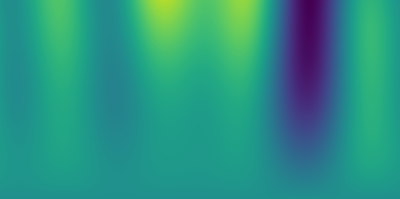
\includegraphics[interpolate=false,width=1.000000in,height=1.000000in]{burgers_exact_diff_0.0-img0.png}}%
\end{pgfscope}%
\begin{pgfscope}%
\pgfsetbuttcap%
\pgfsetroundjoin%
\definecolor{currentfill}{rgb}{0.000000,0.000000,0.000000}%
\pgfsetfillcolor{currentfill}%
\pgfsetlinewidth{0.803000pt}%
\definecolor{currentstroke}{rgb}{0.000000,0.000000,0.000000}%
\pgfsetstrokecolor{currentstroke}%
\pgfsetdash{}{0pt}%
\pgfsys@defobject{currentmarker}{\pgfqpoint{0.000000in}{-0.048611in}}{\pgfqpoint{0.000000in}{0.000000in}}{%
\pgfpathmoveto{\pgfqpoint{0.000000in}{0.000000in}}%
\pgfpathlineto{\pgfqpoint{0.000000in}{-0.048611in}}%
\pgfusepath{stroke,fill}%
}%
\begin{pgfscope}%
\pgfsys@transformshift{0.726837in}{0.517039in}%
\pgfsys@useobject{currentmarker}{}%
\end{pgfscope}%
\end{pgfscope}%
\begin{pgfscope}%
\definecolor{textcolor}{rgb}{0.000000,0.000000,0.000000}%
\pgfsetstrokecolor{textcolor}%
\pgfsetfillcolor{textcolor}%
\pgftext[x=0.726837in,y=0.419816in,,top]{\color{textcolor}\rmfamily\fontsize{12.000000}{14.400000}\selectfont 0}%
\end{pgfscope}%
\begin{pgfscope}%
\pgfsetbuttcap%
\pgfsetroundjoin%
\definecolor{currentfill}{rgb}{0.000000,0.000000,0.000000}%
\pgfsetfillcolor{currentfill}%
\pgfsetlinewidth{0.803000pt}%
\definecolor{currentstroke}{rgb}{0.000000,0.000000,0.000000}%
\pgfsetstrokecolor{currentstroke}%
\pgfsetdash{}{0pt}%
\pgfsys@defobject{currentmarker}{\pgfqpoint{0.000000in}{-0.048611in}}{\pgfqpoint{0.000000in}{0.000000in}}{%
\pgfpathmoveto{\pgfqpoint{0.000000in}{0.000000in}}%
\pgfpathlineto{\pgfqpoint{0.000000in}{-0.048611in}}%
\pgfusepath{stroke,fill}%
}%
\begin{pgfscope}%
\pgfsys@transformshift{1.495229in}{0.517039in}%
\pgfsys@useobject{currentmarker}{}%
\end{pgfscope}%
\end{pgfscope}%
\begin{pgfscope}%
\definecolor{textcolor}{rgb}{0.000000,0.000000,0.000000}%
\pgfsetstrokecolor{textcolor}%
\pgfsetfillcolor{textcolor}%
\pgftext[x=1.495229in,y=0.419816in,,top]{\color{textcolor}\rmfamily\fontsize{12.000000}{14.400000}\selectfont 1}%
\end{pgfscope}%
\begin{pgfscope}%
\pgfsetbuttcap%
\pgfsetroundjoin%
\definecolor{currentfill}{rgb}{0.000000,0.000000,0.000000}%
\pgfsetfillcolor{currentfill}%
\pgfsetlinewidth{0.803000pt}%
\definecolor{currentstroke}{rgb}{0.000000,0.000000,0.000000}%
\pgfsetstrokecolor{currentstroke}%
\pgfsetdash{}{0pt}%
\pgfsys@defobject{currentmarker}{\pgfqpoint{0.000000in}{-0.048611in}}{\pgfqpoint{0.000000in}{0.000000in}}{%
\pgfpathmoveto{\pgfqpoint{0.000000in}{0.000000in}}%
\pgfpathlineto{\pgfqpoint{0.000000in}{-0.048611in}}%
\pgfusepath{stroke,fill}%
}%
\begin{pgfscope}%
\pgfsys@transformshift{2.263621in}{0.517039in}%
\pgfsys@useobject{currentmarker}{}%
\end{pgfscope}%
\end{pgfscope}%
\begin{pgfscope}%
\definecolor{textcolor}{rgb}{0.000000,0.000000,0.000000}%
\pgfsetstrokecolor{textcolor}%
\pgfsetfillcolor{textcolor}%
\pgftext[x=2.263621in,y=0.419816in,,top]{\color{textcolor}\rmfamily\fontsize{12.000000}{14.400000}\selectfont 2}%
\end{pgfscope}%
\begin{pgfscope}%
\definecolor{textcolor}{rgb}{0.000000,0.000000,0.000000}%
\pgfsetstrokecolor{textcolor}%
\pgfsetfillcolor{textcolor}%
\pgftext[x=1.495229in,y=0.202965in,,top]{\color{textcolor}\rmfamily\fontsize{12.000000}{14.400000}\selectfont Space}%
\end{pgfscope}%
\begin{pgfscope}%
\pgfsetbuttcap%
\pgfsetroundjoin%
\definecolor{currentfill}{rgb}{0.000000,0.000000,0.000000}%
\pgfsetfillcolor{currentfill}%
\pgfsetlinewidth{0.803000pt}%
\definecolor{currentstroke}{rgb}{0.000000,0.000000,0.000000}%
\pgfsetstrokecolor{currentstroke}%
\pgfsetdash{}{0pt}%
\pgfsys@defobject{currentmarker}{\pgfqpoint{-0.048611in}{0.000000in}}{\pgfqpoint{-0.000000in}{0.000000in}}{%
\pgfpathmoveto{\pgfqpoint{-0.000000in}{0.000000in}}%
\pgfpathlineto{\pgfqpoint{-0.048611in}{0.000000in}}%
\pgfusepath{stroke,fill}%
}%
\begin{pgfscope}%
\pgfsys@transformshift{0.726837in}{0.517039in}%
\pgfsys@useobject{currentmarker}{}%
\end{pgfscope}%
\end{pgfscope}%
\begin{pgfscope}%
\definecolor{textcolor}{rgb}{0.000000,0.000000,0.000000}%
\pgfsetstrokecolor{textcolor}%
\pgfsetfillcolor{textcolor}%
\pgftext[x=0.364559in, y=0.453725in, left, base]{\color{textcolor}\rmfamily\fontsize{12.000000}{14.400000}\selectfont 0.0}%
\end{pgfscope}%
\begin{pgfscope}%
\pgfsetbuttcap%
\pgfsetroundjoin%
\definecolor{currentfill}{rgb}{0.000000,0.000000,0.000000}%
\pgfsetfillcolor{currentfill}%
\pgfsetlinewidth{0.803000pt}%
\definecolor{currentstroke}{rgb}{0.000000,0.000000,0.000000}%
\pgfsetstrokecolor{currentstroke}%
\pgfsetdash{}{0pt}%
\pgfsys@defobject{currentmarker}{\pgfqpoint{-0.048611in}{0.000000in}}{\pgfqpoint{-0.000000in}{0.000000in}}{%
\pgfpathmoveto{\pgfqpoint{-0.000000in}{0.000000in}}%
\pgfpathlineto{\pgfqpoint{-0.048611in}{0.000000in}}%
\pgfusepath{stroke,fill}%
}%
\begin{pgfscope}%
\pgfsys@transformshift{0.726837in}{0.861533in}%
\pgfsys@useobject{currentmarker}{}%
\end{pgfscope}%
\end{pgfscope}%
\begin{pgfscope}%
\definecolor{textcolor}{rgb}{0.000000,0.000000,0.000000}%
\pgfsetstrokecolor{textcolor}%
\pgfsetfillcolor{textcolor}%
\pgftext[x=0.364559in, y=0.798219in, left, base]{\color{textcolor}\rmfamily\fontsize{12.000000}{14.400000}\selectfont 2.5}%
\end{pgfscope}%
\begin{pgfscope}%
\pgfsetbuttcap%
\pgfsetroundjoin%
\definecolor{currentfill}{rgb}{0.000000,0.000000,0.000000}%
\pgfsetfillcolor{currentfill}%
\pgfsetlinewidth{0.803000pt}%
\definecolor{currentstroke}{rgb}{0.000000,0.000000,0.000000}%
\pgfsetstrokecolor{currentstroke}%
\pgfsetdash{}{0pt}%
\pgfsys@defobject{currentmarker}{\pgfqpoint{-0.048611in}{0.000000in}}{\pgfqpoint{-0.000000in}{0.000000in}}{%
\pgfpathmoveto{\pgfqpoint{-0.000000in}{0.000000in}}%
\pgfpathlineto{\pgfqpoint{-0.048611in}{0.000000in}}%
\pgfusepath{stroke,fill}%
}%
\begin{pgfscope}%
\pgfsys@transformshift{0.726837in}{1.206027in}%
\pgfsys@useobject{currentmarker}{}%
\end{pgfscope}%
\end{pgfscope}%
\begin{pgfscope}%
\definecolor{textcolor}{rgb}{0.000000,0.000000,0.000000}%
\pgfsetstrokecolor{textcolor}%
\pgfsetfillcolor{textcolor}%
\pgftext[x=0.364559in, y=1.142714in, left, base]{\color{textcolor}\rmfamily\fontsize{12.000000}{14.400000}\selectfont 5.0}%
\end{pgfscope}%
\begin{pgfscope}%
\pgfsetbuttcap%
\pgfsetroundjoin%
\definecolor{currentfill}{rgb}{0.000000,0.000000,0.000000}%
\pgfsetfillcolor{currentfill}%
\pgfsetlinewidth{0.803000pt}%
\definecolor{currentstroke}{rgb}{0.000000,0.000000,0.000000}%
\pgfsetstrokecolor{currentstroke}%
\pgfsetdash{}{0pt}%
\pgfsys@defobject{currentmarker}{\pgfqpoint{-0.048611in}{0.000000in}}{\pgfqpoint{-0.000000in}{0.000000in}}{%
\pgfpathmoveto{\pgfqpoint{-0.000000in}{0.000000in}}%
\pgfpathlineto{\pgfqpoint{-0.048611in}{0.000000in}}%
\pgfusepath{stroke,fill}%
}%
\begin{pgfscope}%
\pgfsys@transformshift{0.726837in}{1.550522in}%
\pgfsys@useobject{currentmarker}{}%
\end{pgfscope}%
\end{pgfscope}%
\begin{pgfscope}%
\definecolor{textcolor}{rgb}{0.000000,0.000000,0.000000}%
\pgfsetstrokecolor{textcolor}%
\pgfsetfillcolor{textcolor}%
\pgftext[x=0.364559in, y=1.487208in, left, base]{\color{textcolor}\rmfamily\fontsize{12.000000}{14.400000}\selectfont 7.5}%
\end{pgfscope}%
\begin{pgfscope}%
\pgfsetbuttcap%
\pgfsetroundjoin%
\definecolor{currentfill}{rgb}{0.000000,0.000000,0.000000}%
\pgfsetfillcolor{currentfill}%
\pgfsetlinewidth{0.803000pt}%
\definecolor{currentstroke}{rgb}{0.000000,0.000000,0.000000}%
\pgfsetstrokecolor{currentstroke}%
\pgfsetdash{}{0pt}%
\pgfsys@defobject{currentmarker}{\pgfqpoint{-0.048611in}{0.000000in}}{\pgfqpoint{-0.000000in}{0.000000in}}{%
\pgfpathmoveto{\pgfqpoint{-0.000000in}{0.000000in}}%
\pgfpathlineto{\pgfqpoint{-0.048611in}{0.000000in}}%
\pgfusepath{stroke,fill}%
}%
\begin{pgfscope}%
\pgfsys@transformshift{0.726837in}{1.895016in}%
\pgfsys@useobject{currentmarker}{}%
\end{pgfscope}%
\end{pgfscope}%
\begin{pgfscope}%
\definecolor{textcolor}{rgb}{0.000000,0.000000,0.000000}%
\pgfsetstrokecolor{textcolor}%
\pgfsetfillcolor{textcolor}%
\pgftext[x=0.258521in, y=1.831702in, left, base]{\color{textcolor}\rmfamily\fontsize{12.000000}{14.400000}\selectfont 10.0}%
\end{pgfscope}%
\begin{pgfscope}%
\definecolor{textcolor}{rgb}{0.000000,0.000000,0.000000}%
\pgfsetstrokecolor{textcolor}%
\pgfsetfillcolor{textcolor}%
\pgftext[x=0.202965in,y=1.206027in,,bottom,rotate=90.000000]{\color{textcolor}\rmfamily\fontsize{12.000000}{14.400000}\selectfont Time}%
\end{pgfscope}%
\begin{pgfscope}%
\pgfsetrectcap%
\pgfsetmiterjoin%
\pgfsetlinewidth{0.803000pt}%
\definecolor{currentstroke}{rgb}{0.000000,0.000000,0.000000}%
\pgfsetstrokecolor{currentstroke}%
\pgfsetdash{}{0pt}%
\pgfpathmoveto{\pgfqpoint{0.726837in}{0.517039in}}%
\pgfpathlineto{\pgfqpoint{0.726837in}{1.895016in}}%
\pgfusepath{stroke}%
\end{pgfscope}%
\begin{pgfscope}%
\pgfsetrectcap%
\pgfsetmiterjoin%
\pgfsetlinewidth{0.803000pt}%
\definecolor{currentstroke}{rgb}{0.000000,0.000000,0.000000}%
\pgfsetstrokecolor{currentstroke}%
\pgfsetdash{}{0pt}%
\pgfpathmoveto{\pgfqpoint{2.263621in}{0.517039in}}%
\pgfpathlineto{\pgfqpoint{2.263621in}{1.895016in}}%
\pgfusepath{stroke}%
\end{pgfscope}%
\begin{pgfscope}%
\pgfsetrectcap%
\pgfsetmiterjoin%
\pgfsetlinewidth{0.803000pt}%
\definecolor{currentstroke}{rgb}{0.000000,0.000000,0.000000}%
\pgfsetstrokecolor{currentstroke}%
\pgfsetdash{}{0pt}%
\pgfpathmoveto{\pgfqpoint{0.726837in}{0.517039in}}%
\pgfpathlineto{\pgfqpoint{2.263621in}{0.517039in}}%
\pgfusepath{stroke}%
\end{pgfscope}%
\begin{pgfscope}%
\pgfsetrectcap%
\pgfsetmiterjoin%
\pgfsetlinewidth{0.803000pt}%
\definecolor{currentstroke}{rgb}{0.000000,0.000000,0.000000}%
\pgfsetstrokecolor{currentstroke}%
\pgfsetdash{}{0pt}%
\pgfpathmoveto{\pgfqpoint{0.726837in}{1.895016in}}%
\pgfpathlineto{\pgfqpoint{2.263621in}{1.895016in}}%
\pgfusepath{stroke}%
\end{pgfscope}%
\begin{pgfscope}%
\pgfsetbuttcap%
\pgfsetmiterjoin%
\pgfsetlinewidth{0.000000pt}%
\definecolor{currentstroke}{rgb}{0.000000,0.000000,0.000000}%
\pgfsetstrokecolor{currentstroke}%
\pgfsetstrokeopacity{0.000000}%
\pgfsetdash{}{0pt}%
\pgfpathmoveto{\pgfqpoint{2.393479in}{0.517039in}}%
\pgfpathlineto{\pgfqpoint{2.462378in}{0.517039in}}%
\pgfpathlineto{\pgfqpoint{2.462378in}{1.895016in}}%
\pgfpathlineto{\pgfqpoint{2.393479in}{1.895016in}}%
\pgfpathlineto{\pgfqpoint{2.393479in}{0.517039in}}%
\pgfpathclose%
\pgfusepath{}%
\end{pgfscope}%
\begin{pgfscope}%
\pgfsys@transformshift{2.390000in}{0.520000in}%
\pgftext[left,bottom]{
\includegraphics[interpolate=true,width=0.070000in,height=1.380000in]{burgers_exact_diff_0.0-img1.png}}%
\end{pgfscope}%
\begin{pgfscope}%
\pgfsetbuttcap%
\pgfsetroundjoin%
\definecolor{currentfill}{rgb}{0.000000,0.000000,0.000000}%
\pgfsetfillcolor{currentfill}%
\pgfsetlinewidth{0.803000pt}%
\definecolor{currentstroke}{rgb}{0.000000,0.000000,0.000000}%
\pgfsetstrokecolor{currentstroke}%
\pgfsetdash{}{0pt}%
\pgfsys@defobject{currentmarker}{\pgfqpoint{0.000000in}{0.000000in}}{\pgfqpoint{0.048611in}{0.000000in}}{%
\pgfpathmoveto{\pgfqpoint{0.000000in}{0.000000in}}%
\pgfpathlineto{\pgfqpoint{0.048611in}{0.000000in}}%
\pgfusepath{stroke,fill}%
}%
\begin{pgfscope}%
\pgfsys@transformshift{2.462378in}{0.565953in}%
\pgfsys@useobject{currentmarker}{}%
\end{pgfscope}%
\end{pgfscope}%
\begin{pgfscope}%
\definecolor{textcolor}{rgb}{0.000000,0.000000,0.000000}%
\pgfsetstrokecolor{textcolor}%
\pgfsetfillcolor{textcolor}%
\pgftext[x=2.559601in, y=0.502639in, left, base]{\color{textcolor}\rmfamily\fontsize{12.000000}{14.400000}\selectfont \ensuremath{-}0.2}%
\end{pgfscope}%
\begin{pgfscope}%
\pgfsetbuttcap%
\pgfsetroundjoin%
\definecolor{currentfill}{rgb}{0.000000,0.000000,0.000000}%
\pgfsetfillcolor{currentfill}%
\pgfsetlinewidth{0.803000pt}%
\definecolor{currentstroke}{rgb}{0.000000,0.000000,0.000000}%
\pgfsetstrokecolor{currentstroke}%
\pgfsetdash{}{0pt}%
\pgfsys@defobject{currentmarker}{\pgfqpoint{0.000000in}{0.000000in}}{\pgfqpoint{0.048611in}{0.000000in}}{%
\pgfpathmoveto{\pgfqpoint{0.000000in}{0.000000in}}%
\pgfpathlineto{\pgfqpoint{0.048611in}{0.000000in}}%
\pgfusepath{stroke,fill}%
}%
\begin{pgfscope}%
\pgfsys@transformshift{2.462378in}{1.206027in}%
\pgfsys@useobject{currentmarker}{}%
\end{pgfscope}%
\end{pgfscope}%
\begin{pgfscope}%
\definecolor{textcolor}{rgb}{0.000000,0.000000,0.000000}%
\pgfsetstrokecolor{textcolor}%
\pgfsetfillcolor{textcolor}%
\pgftext[x=2.559601in, y=1.142714in, left, base]{\color{textcolor}\rmfamily\fontsize{12.000000}{14.400000}\selectfont 0.0}%
\end{pgfscope}%
\begin{pgfscope}%
\pgfsetbuttcap%
\pgfsetroundjoin%
\definecolor{currentfill}{rgb}{0.000000,0.000000,0.000000}%
\pgfsetfillcolor{currentfill}%
\pgfsetlinewidth{0.803000pt}%
\definecolor{currentstroke}{rgb}{0.000000,0.000000,0.000000}%
\pgfsetstrokecolor{currentstroke}%
\pgfsetdash{}{0pt}%
\pgfsys@defobject{currentmarker}{\pgfqpoint{0.000000in}{0.000000in}}{\pgfqpoint{0.048611in}{0.000000in}}{%
\pgfpathmoveto{\pgfqpoint{0.000000in}{0.000000in}}%
\pgfpathlineto{\pgfqpoint{0.048611in}{0.000000in}}%
\pgfusepath{stroke,fill}%
}%
\begin{pgfscope}%
\pgfsys@transformshift{2.462378in}{1.846102in}%
\pgfsys@useobject{currentmarker}{}%
\end{pgfscope}%
\end{pgfscope}%
\begin{pgfscope}%
\definecolor{textcolor}{rgb}{0.000000,0.000000,0.000000}%
\pgfsetstrokecolor{textcolor}%
\pgfsetfillcolor{textcolor}%
\pgftext[x=2.559601in, y=1.782788in, left, base]{\color{textcolor}\rmfamily\fontsize{12.000000}{14.400000}\selectfont 0.2}%
\end{pgfscope}%
\begin{pgfscope}%
\pgfsetrectcap%
\pgfsetmiterjoin%
\pgfsetlinewidth{0.803000pt}%
\definecolor{currentstroke}{rgb}{0.000000,0.000000,0.000000}%
\pgfsetstrokecolor{currentstroke}%
\pgfsetdash{}{0pt}%
\pgfpathmoveto{\pgfqpoint{2.393479in}{0.517039in}}%
\pgfpathlineto{\pgfqpoint{2.427929in}{0.517039in}}%
\pgfpathlineto{\pgfqpoint{2.462378in}{0.517039in}}%
\pgfpathlineto{\pgfqpoint{2.462378in}{1.895016in}}%
\pgfpathlineto{\pgfqpoint{2.427929in}{1.895016in}}%
\pgfpathlineto{\pgfqpoint{2.393479in}{1.895016in}}%
\pgfpathlineto{\pgfqpoint{2.393479in}{0.517039in}}%
\pgfpathclose%
\pgfusepath{stroke}%
\end{pgfscope}%
\end{pgfpicture}%
\makeatother%
\endgroup%

      \end{adjustbox}
      \caption{The difference for \(\nu=0.0\)}\label{fig:sc2_exact_diff_0.0}
    \end{subfigure}
    \\[0.7\baselineskip]
    \begin{subfigure}{0.33\linewidth}
      \begin{adjustbox}{width=\linewidth}
        \begingroup%
\makeatletter%
\begin{pgfpicture}%
\pgfpathrectangle{\pgfpointorigin}{\pgfqpoint{3.000000in}{2.000000in}}%
\pgfusepath{use as bounding box, clip}%
\begin{pgfscope}%
\pgfsetbuttcap%
\pgfsetmiterjoin%
\pgfsetlinewidth{0.000000pt}%
\definecolor{currentstroke}{rgb}{0.000000,0.000000,0.000000}%
\pgfsetstrokecolor{currentstroke}%
\pgfsetstrokeopacity{0.000000}%
\pgfsetdash{}{0pt}%
\pgfpathmoveto{\pgfqpoint{0.000000in}{0.000000in}}%
\pgfpathlineto{\pgfqpoint{3.000000in}{0.000000in}}%
\pgfpathlineto{\pgfqpoint{3.000000in}{2.000000in}}%
\pgfpathlineto{\pgfqpoint{0.000000in}{2.000000in}}%
\pgfpathlineto{\pgfqpoint{0.000000in}{0.000000in}}%
\pgfpathclose%
\pgfusepath{}%
\end{pgfscope}%
\begin{pgfscope}%
\pgfsetbuttcap%
\pgfsetmiterjoin%
\pgfsetlinewidth{0.000000pt}%
\definecolor{currentstroke}{rgb}{0.000000,0.000000,0.000000}%
\pgfsetstrokecolor{currentstroke}%
\pgfsetstrokeopacity{0.000000}%
\pgfsetdash{}{0pt}%
\pgfpathmoveto{\pgfqpoint{0.726837in}{0.517039in}}%
\pgfpathlineto{\pgfqpoint{2.263621in}{0.517039in}}%
\pgfpathlineto{\pgfqpoint{2.263621in}{1.895016in}}%
\pgfpathlineto{\pgfqpoint{0.726837in}{1.895016in}}%
\pgfpathlineto{\pgfqpoint{0.726837in}{0.517039in}}%
\pgfpathclose%
\pgfusepath{}%
\end{pgfscope}%
\begin{pgfscope}%
\pgfpathrectangle{\pgfqpoint{0.726837in}{0.517039in}}{\pgfqpoint{1.536784in}{1.377978in}}%
\pgfusepath{clip}%
\pgfsys@transformcm{1.536784}{0.000000}{0.000000}{1.377978}{0.726837in}{0.517039in}%
\pgftext[left,bottom]{
\includegraphics[interpolate=false,width=1.000000in,height=1.000000in]{burgers_exact_target_0.01-img0.png}}%
\end{pgfscope}%
\begin{pgfscope}%
\pgfsetbuttcap%
\pgfsetroundjoin%
\definecolor{currentfill}{rgb}{0.000000,0.000000,0.000000}%
\pgfsetfillcolor{currentfill}%
\pgfsetlinewidth{0.803000pt}%
\definecolor{currentstroke}{rgb}{0.000000,0.000000,0.000000}%
\pgfsetstrokecolor{currentstroke}%
\pgfsetdash{}{0pt}%
\pgfsys@defobject{currentmarker}{\pgfqpoint{0.000000in}{-0.048611in}}{\pgfqpoint{0.000000in}{0.000000in}}{%
\pgfpathmoveto{\pgfqpoint{0.000000in}{0.000000in}}%
\pgfpathlineto{\pgfqpoint{0.000000in}{-0.048611in}}%
\pgfusepath{stroke,fill}%
}%
\begin{pgfscope}%
\pgfsys@transformshift{0.726837in}{0.517039in}%
\pgfsys@useobject{currentmarker}{}%
\end{pgfscope}%
\end{pgfscope}%
\begin{pgfscope}%
\definecolor{textcolor}{rgb}{0.000000,0.000000,0.000000}%
\pgfsetstrokecolor{textcolor}%
\pgfsetfillcolor{textcolor}%
\pgftext[x=0.726837in,y=0.419816in,,top]{\color{textcolor}\rmfamily\fontsize{12.000000}{14.400000}\selectfont 0}%
\end{pgfscope}%
\begin{pgfscope}%
\pgfsetbuttcap%
\pgfsetroundjoin%
\definecolor{currentfill}{rgb}{0.000000,0.000000,0.000000}%
\pgfsetfillcolor{currentfill}%
\pgfsetlinewidth{0.803000pt}%
\definecolor{currentstroke}{rgb}{0.000000,0.000000,0.000000}%
\pgfsetstrokecolor{currentstroke}%
\pgfsetdash{}{0pt}%
\pgfsys@defobject{currentmarker}{\pgfqpoint{0.000000in}{-0.048611in}}{\pgfqpoint{0.000000in}{0.000000in}}{%
\pgfpathmoveto{\pgfqpoint{0.000000in}{0.000000in}}%
\pgfpathlineto{\pgfqpoint{0.000000in}{-0.048611in}}%
\pgfusepath{stroke,fill}%
}%
\begin{pgfscope}%
\pgfsys@transformshift{1.495229in}{0.517039in}%
\pgfsys@useobject{currentmarker}{}%
\end{pgfscope}%
\end{pgfscope}%
\begin{pgfscope}%
\definecolor{textcolor}{rgb}{0.000000,0.000000,0.000000}%
\pgfsetstrokecolor{textcolor}%
\pgfsetfillcolor{textcolor}%
\pgftext[x=1.495229in,y=0.419816in,,top]{\color{textcolor}\rmfamily\fontsize{12.000000}{14.400000}\selectfont 1}%
\end{pgfscope}%
\begin{pgfscope}%
\pgfsetbuttcap%
\pgfsetroundjoin%
\definecolor{currentfill}{rgb}{0.000000,0.000000,0.000000}%
\pgfsetfillcolor{currentfill}%
\pgfsetlinewidth{0.803000pt}%
\definecolor{currentstroke}{rgb}{0.000000,0.000000,0.000000}%
\pgfsetstrokecolor{currentstroke}%
\pgfsetdash{}{0pt}%
\pgfsys@defobject{currentmarker}{\pgfqpoint{0.000000in}{-0.048611in}}{\pgfqpoint{0.000000in}{0.000000in}}{%
\pgfpathmoveto{\pgfqpoint{0.000000in}{0.000000in}}%
\pgfpathlineto{\pgfqpoint{0.000000in}{-0.048611in}}%
\pgfusepath{stroke,fill}%
}%
\begin{pgfscope}%
\pgfsys@transformshift{2.263621in}{0.517039in}%
\pgfsys@useobject{currentmarker}{}%
\end{pgfscope}%
\end{pgfscope}%
\begin{pgfscope}%
\definecolor{textcolor}{rgb}{0.000000,0.000000,0.000000}%
\pgfsetstrokecolor{textcolor}%
\pgfsetfillcolor{textcolor}%
\pgftext[x=2.263621in,y=0.419816in,,top]{\color{textcolor}\rmfamily\fontsize{12.000000}{14.400000}\selectfont 2}%
\end{pgfscope}%
\begin{pgfscope}%
\definecolor{textcolor}{rgb}{0.000000,0.000000,0.000000}%
\pgfsetstrokecolor{textcolor}%
\pgfsetfillcolor{textcolor}%
\pgftext[x=1.495229in,y=0.202965in,,top]{\color{textcolor}\rmfamily\fontsize{12.000000}{14.400000}\selectfont Space}%
\end{pgfscope}%
\begin{pgfscope}%
\pgfsetbuttcap%
\pgfsetroundjoin%
\definecolor{currentfill}{rgb}{0.000000,0.000000,0.000000}%
\pgfsetfillcolor{currentfill}%
\pgfsetlinewidth{0.803000pt}%
\definecolor{currentstroke}{rgb}{0.000000,0.000000,0.000000}%
\pgfsetstrokecolor{currentstroke}%
\pgfsetdash{}{0pt}%
\pgfsys@defobject{currentmarker}{\pgfqpoint{-0.048611in}{0.000000in}}{\pgfqpoint{-0.000000in}{0.000000in}}{%
\pgfpathmoveto{\pgfqpoint{-0.000000in}{0.000000in}}%
\pgfpathlineto{\pgfqpoint{-0.048611in}{0.000000in}}%
\pgfusepath{stroke,fill}%
}%
\begin{pgfscope}%
\pgfsys@transformshift{0.726837in}{0.517039in}%
\pgfsys@useobject{currentmarker}{}%
\end{pgfscope}%
\end{pgfscope}%
\begin{pgfscope}%
\definecolor{textcolor}{rgb}{0.000000,0.000000,0.000000}%
\pgfsetstrokecolor{textcolor}%
\pgfsetfillcolor{textcolor}%
\pgftext[x=0.364559in, y=0.453725in, left, base]{\color{textcolor}\rmfamily\fontsize{12.000000}{14.400000}\selectfont 0.0}%
\end{pgfscope}%
\begin{pgfscope}%
\pgfsetbuttcap%
\pgfsetroundjoin%
\definecolor{currentfill}{rgb}{0.000000,0.000000,0.000000}%
\pgfsetfillcolor{currentfill}%
\pgfsetlinewidth{0.803000pt}%
\definecolor{currentstroke}{rgb}{0.000000,0.000000,0.000000}%
\pgfsetstrokecolor{currentstroke}%
\pgfsetdash{}{0pt}%
\pgfsys@defobject{currentmarker}{\pgfqpoint{-0.048611in}{0.000000in}}{\pgfqpoint{-0.000000in}{0.000000in}}{%
\pgfpathmoveto{\pgfqpoint{-0.000000in}{0.000000in}}%
\pgfpathlineto{\pgfqpoint{-0.048611in}{0.000000in}}%
\pgfusepath{stroke,fill}%
}%
\begin{pgfscope}%
\pgfsys@transformshift{0.726837in}{0.861533in}%
\pgfsys@useobject{currentmarker}{}%
\end{pgfscope}%
\end{pgfscope}%
\begin{pgfscope}%
\definecolor{textcolor}{rgb}{0.000000,0.000000,0.000000}%
\pgfsetstrokecolor{textcolor}%
\pgfsetfillcolor{textcolor}%
\pgftext[x=0.364559in, y=0.798219in, left, base]{\color{textcolor}\rmfamily\fontsize{12.000000}{14.400000}\selectfont 2.5}%
\end{pgfscope}%
\begin{pgfscope}%
\pgfsetbuttcap%
\pgfsetroundjoin%
\definecolor{currentfill}{rgb}{0.000000,0.000000,0.000000}%
\pgfsetfillcolor{currentfill}%
\pgfsetlinewidth{0.803000pt}%
\definecolor{currentstroke}{rgb}{0.000000,0.000000,0.000000}%
\pgfsetstrokecolor{currentstroke}%
\pgfsetdash{}{0pt}%
\pgfsys@defobject{currentmarker}{\pgfqpoint{-0.048611in}{0.000000in}}{\pgfqpoint{-0.000000in}{0.000000in}}{%
\pgfpathmoveto{\pgfqpoint{-0.000000in}{0.000000in}}%
\pgfpathlineto{\pgfqpoint{-0.048611in}{0.000000in}}%
\pgfusepath{stroke,fill}%
}%
\begin{pgfscope}%
\pgfsys@transformshift{0.726837in}{1.206027in}%
\pgfsys@useobject{currentmarker}{}%
\end{pgfscope}%
\end{pgfscope}%
\begin{pgfscope}%
\definecolor{textcolor}{rgb}{0.000000,0.000000,0.000000}%
\pgfsetstrokecolor{textcolor}%
\pgfsetfillcolor{textcolor}%
\pgftext[x=0.364559in, y=1.142714in, left, base]{\color{textcolor}\rmfamily\fontsize{12.000000}{14.400000}\selectfont 5.0}%
\end{pgfscope}%
\begin{pgfscope}%
\pgfsetbuttcap%
\pgfsetroundjoin%
\definecolor{currentfill}{rgb}{0.000000,0.000000,0.000000}%
\pgfsetfillcolor{currentfill}%
\pgfsetlinewidth{0.803000pt}%
\definecolor{currentstroke}{rgb}{0.000000,0.000000,0.000000}%
\pgfsetstrokecolor{currentstroke}%
\pgfsetdash{}{0pt}%
\pgfsys@defobject{currentmarker}{\pgfqpoint{-0.048611in}{0.000000in}}{\pgfqpoint{-0.000000in}{0.000000in}}{%
\pgfpathmoveto{\pgfqpoint{-0.000000in}{0.000000in}}%
\pgfpathlineto{\pgfqpoint{-0.048611in}{0.000000in}}%
\pgfusepath{stroke,fill}%
}%
\begin{pgfscope}%
\pgfsys@transformshift{0.726837in}{1.550522in}%
\pgfsys@useobject{currentmarker}{}%
\end{pgfscope}%
\end{pgfscope}%
\begin{pgfscope}%
\definecolor{textcolor}{rgb}{0.000000,0.000000,0.000000}%
\pgfsetstrokecolor{textcolor}%
\pgfsetfillcolor{textcolor}%
\pgftext[x=0.364559in, y=1.487208in, left, base]{\color{textcolor}\rmfamily\fontsize{12.000000}{14.400000}\selectfont 7.5}%
\end{pgfscope}%
\begin{pgfscope}%
\pgfsetbuttcap%
\pgfsetroundjoin%
\definecolor{currentfill}{rgb}{0.000000,0.000000,0.000000}%
\pgfsetfillcolor{currentfill}%
\pgfsetlinewidth{0.803000pt}%
\definecolor{currentstroke}{rgb}{0.000000,0.000000,0.000000}%
\pgfsetstrokecolor{currentstroke}%
\pgfsetdash{}{0pt}%
\pgfsys@defobject{currentmarker}{\pgfqpoint{-0.048611in}{0.000000in}}{\pgfqpoint{-0.000000in}{0.000000in}}{%
\pgfpathmoveto{\pgfqpoint{-0.000000in}{0.000000in}}%
\pgfpathlineto{\pgfqpoint{-0.048611in}{0.000000in}}%
\pgfusepath{stroke,fill}%
}%
\begin{pgfscope}%
\pgfsys@transformshift{0.726837in}{1.895016in}%
\pgfsys@useobject{currentmarker}{}%
\end{pgfscope}%
\end{pgfscope}%
\begin{pgfscope}%
\definecolor{textcolor}{rgb}{0.000000,0.000000,0.000000}%
\pgfsetstrokecolor{textcolor}%
\pgfsetfillcolor{textcolor}%
\pgftext[x=0.258521in, y=1.831702in, left, base]{\color{textcolor}\rmfamily\fontsize{12.000000}{14.400000}\selectfont 10.0}%
\end{pgfscope}%
\begin{pgfscope}%
\definecolor{textcolor}{rgb}{0.000000,0.000000,0.000000}%
\pgfsetstrokecolor{textcolor}%
\pgfsetfillcolor{textcolor}%
\pgftext[x=0.202965in,y=1.206027in,,bottom,rotate=90.000000]{\color{textcolor}\rmfamily\fontsize{12.000000}{14.400000}\selectfont Time}%
\end{pgfscope}%
\begin{pgfscope}%
\pgfsetrectcap%
\pgfsetmiterjoin%
\pgfsetlinewidth{0.803000pt}%
\definecolor{currentstroke}{rgb}{0.000000,0.000000,0.000000}%
\pgfsetstrokecolor{currentstroke}%
\pgfsetdash{}{0pt}%
\pgfpathmoveto{\pgfqpoint{0.726837in}{0.517039in}}%
\pgfpathlineto{\pgfqpoint{0.726837in}{1.895016in}}%
\pgfusepath{stroke}%
\end{pgfscope}%
\begin{pgfscope}%
\pgfsetrectcap%
\pgfsetmiterjoin%
\pgfsetlinewidth{0.803000pt}%
\definecolor{currentstroke}{rgb}{0.000000,0.000000,0.000000}%
\pgfsetstrokecolor{currentstroke}%
\pgfsetdash{}{0pt}%
\pgfpathmoveto{\pgfqpoint{2.263621in}{0.517039in}}%
\pgfpathlineto{\pgfqpoint{2.263621in}{1.895016in}}%
\pgfusepath{stroke}%
\end{pgfscope}%
\begin{pgfscope}%
\pgfsetrectcap%
\pgfsetmiterjoin%
\pgfsetlinewidth{0.803000pt}%
\definecolor{currentstroke}{rgb}{0.000000,0.000000,0.000000}%
\pgfsetstrokecolor{currentstroke}%
\pgfsetdash{}{0pt}%
\pgfpathmoveto{\pgfqpoint{0.726837in}{0.517039in}}%
\pgfpathlineto{\pgfqpoint{2.263621in}{0.517039in}}%
\pgfusepath{stroke}%
\end{pgfscope}%
\begin{pgfscope}%
\pgfsetrectcap%
\pgfsetmiterjoin%
\pgfsetlinewidth{0.803000pt}%
\definecolor{currentstroke}{rgb}{0.000000,0.000000,0.000000}%
\pgfsetstrokecolor{currentstroke}%
\pgfsetdash{}{0pt}%
\pgfpathmoveto{\pgfqpoint{0.726837in}{1.895016in}}%
\pgfpathlineto{\pgfqpoint{2.263621in}{1.895016in}}%
\pgfusepath{stroke}%
\end{pgfscope}%
\begin{pgfscope}%
\pgfsetbuttcap%
\pgfsetmiterjoin%
\pgfsetlinewidth{0.000000pt}%
\definecolor{currentstroke}{rgb}{0.000000,0.000000,0.000000}%
\pgfsetstrokecolor{currentstroke}%
\pgfsetstrokeopacity{0.000000}%
\pgfsetdash{}{0pt}%
\pgfpathmoveto{\pgfqpoint{2.393479in}{0.517039in}}%
\pgfpathlineto{\pgfqpoint{2.462378in}{0.517039in}}%
\pgfpathlineto{\pgfqpoint{2.462378in}{1.895016in}}%
\pgfpathlineto{\pgfqpoint{2.393479in}{1.895016in}}%
\pgfpathlineto{\pgfqpoint{2.393479in}{0.517039in}}%
\pgfpathclose%
\pgfusepath{}%
\end{pgfscope}%
\begin{pgfscope}%
\pgfsys@transformshift{2.390000in}{0.520000in}%
\pgftext[left,bottom]{
\includegraphics[interpolate=true,width=0.070000in,height=1.380000in]{burgers_exact_target_0.01-img1.png}}%
\end{pgfscope}%
\begin{pgfscope}%
\pgfsetbuttcap%
\pgfsetroundjoin%
\definecolor{currentfill}{rgb}{0.000000,0.000000,0.000000}%
\pgfsetfillcolor{currentfill}%
\pgfsetlinewidth{0.803000pt}%
\definecolor{currentstroke}{rgb}{0.000000,0.000000,0.000000}%
\pgfsetstrokecolor{currentstroke}%
\pgfsetdash{}{0pt}%
\pgfsys@defobject{currentmarker}{\pgfqpoint{0.000000in}{0.000000in}}{\pgfqpoint{0.048611in}{0.000000in}}{%
\pgfpathmoveto{\pgfqpoint{0.000000in}{0.000000in}}%
\pgfpathlineto{\pgfqpoint{0.048611in}{0.000000in}}%
\pgfusepath{stroke,fill}%
}%
\begin{pgfscope}%
\pgfsys@transformshift{2.462378in}{0.649681in}%
\pgfsys@useobject{currentmarker}{}%
\end{pgfscope}%
\end{pgfscope}%
\begin{pgfscope}%
\definecolor{textcolor}{rgb}{0.000000,0.000000,0.000000}%
\pgfsetstrokecolor{textcolor}%
\pgfsetfillcolor{textcolor}%
\pgftext[x=2.559601in, y=0.586367in, left, base]{\color{textcolor}\rmfamily\fontsize{12.000000}{14.400000}\selectfont \ensuremath{-}0.1}%
\end{pgfscope}%
\begin{pgfscope}%
\pgfsetbuttcap%
\pgfsetroundjoin%
\definecolor{currentfill}{rgb}{0.000000,0.000000,0.000000}%
\pgfsetfillcolor{currentfill}%
\pgfsetlinewidth{0.803000pt}%
\definecolor{currentstroke}{rgb}{0.000000,0.000000,0.000000}%
\pgfsetstrokecolor{currentstroke}%
\pgfsetdash{}{0pt}%
\pgfsys@defobject{currentmarker}{\pgfqpoint{0.000000in}{0.000000in}}{\pgfqpoint{0.048611in}{0.000000in}}{%
\pgfpathmoveto{\pgfqpoint{0.000000in}{0.000000in}}%
\pgfpathlineto{\pgfqpoint{0.048611in}{0.000000in}}%
\pgfusepath{stroke,fill}%
}%
\begin{pgfscope}%
\pgfsys@transformshift{2.462378in}{1.206027in}%
\pgfsys@useobject{currentmarker}{}%
\end{pgfscope}%
\end{pgfscope}%
\begin{pgfscope}%
\definecolor{textcolor}{rgb}{0.000000,0.000000,0.000000}%
\pgfsetstrokecolor{textcolor}%
\pgfsetfillcolor{textcolor}%
\pgftext[x=2.559601in, y=1.142714in, left, base]{\color{textcolor}\rmfamily\fontsize{12.000000}{14.400000}\selectfont 0.0}%
\end{pgfscope}%
\begin{pgfscope}%
\pgfsetbuttcap%
\pgfsetroundjoin%
\definecolor{currentfill}{rgb}{0.000000,0.000000,0.000000}%
\pgfsetfillcolor{currentfill}%
\pgfsetlinewidth{0.803000pt}%
\definecolor{currentstroke}{rgb}{0.000000,0.000000,0.000000}%
\pgfsetstrokecolor{currentstroke}%
\pgfsetdash{}{0pt}%
\pgfsys@defobject{currentmarker}{\pgfqpoint{0.000000in}{0.000000in}}{\pgfqpoint{0.048611in}{0.000000in}}{%
\pgfpathmoveto{\pgfqpoint{0.000000in}{0.000000in}}%
\pgfpathlineto{\pgfqpoint{0.048611in}{0.000000in}}%
\pgfusepath{stroke,fill}%
}%
\begin{pgfscope}%
\pgfsys@transformshift{2.462378in}{1.762374in}%
\pgfsys@useobject{currentmarker}{}%
\end{pgfscope}%
\end{pgfscope}%
\begin{pgfscope}%
\definecolor{textcolor}{rgb}{0.000000,0.000000,0.000000}%
\pgfsetstrokecolor{textcolor}%
\pgfsetfillcolor{textcolor}%
\pgftext[x=2.559601in, y=1.699060in, left, base]{\color{textcolor}\rmfamily\fontsize{12.000000}{14.400000}\selectfont 0.1}%
\end{pgfscope}%
\begin{pgfscope}%
\pgfsetrectcap%
\pgfsetmiterjoin%
\pgfsetlinewidth{0.803000pt}%
\definecolor{currentstroke}{rgb}{0.000000,0.000000,0.000000}%
\pgfsetstrokecolor{currentstroke}%
\pgfsetdash{}{0pt}%
\pgfpathmoveto{\pgfqpoint{2.393479in}{0.517039in}}%
\pgfpathlineto{\pgfqpoint{2.427929in}{0.517039in}}%
\pgfpathlineto{\pgfqpoint{2.462378in}{0.517039in}}%
\pgfpathlineto{\pgfqpoint{2.462378in}{1.895016in}}%
\pgfpathlineto{\pgfqpoint{2.427929in}{1.895016in}}%
\pgfpathlineto{\pgfqpoint{2.393479in}{1.895016in}}%
\pgfpathlineto{\pgfqpoint{2.393479in}{0.517039in}}%
\pgfpathclose%
\pgfusepath{stroke}%
\end{pgfscope}%
\end{pgfpicture}%
\makeatother%
\endgroup%

      \end{adjustbox}
      \caption{The target for \(\nu=0.01\)}\label{fig:sc2_exact_target_0.01}
    \end{subfigure}
    \begin{subfigure}{0.33\linewidth}
      \begin{adjustbox}{width=\linewidth}
        \begingroup%
\makeatletter%
\begin{pgfpicture}%
\pgfpathrectangle{\pgfpointorigin}{\pgfqpoint{3.000000in}{2.000000in}}%
\pgfusepath{use as bounding box, clip}%
\begin{pgfscope}%
\pgfsetbuttcap%
\pgfsetmiterjoin%
\pgfsetlinewidth{0.000000pt}%
\definecolor{currentstroke}{rgb}{0.000000,0.000000,0.000000}%
\pgfsetstrokecolor{currentstroke}%
\pgfsetstrokeopacity{0.000000}%
\pgfsetdash{}{0pt}%
\pgfpathmoveto{\pgfqpoint{0.000000in}{0.000000in}}%
\pgfpathlineto{\pgfqpoint{3.000000in}{0.000000in}}%
\pgfpathlineto{\pgfqpoint{3.000000in}{2.000000in}}%
\pgfpathlineto{\pgfqpoint{0.000000in}{2.000000in}}%
\pgfpathlineto{\pgfqpoint{0.000000in}{0.000000in}}%
\pgfpathclose%
\pgfusepath{}%
\end{pgfscope}%
\begin{pgfscope}%
\pgfsetbuttcap%
\pgfsetmiterjoin%
\pgfsetlinewidth{0.000000pt}%
\definecolor{currentstroke}{rgb}{0.000000,0.000000,0.000000}%
\pgfsetstrokecolor{currentstroke}%
\pgfsetstrokeopacity{0.000000}%
\pgfsetdash{}{0pt}%
\pgfpathmoveto{\pgfqpoint{0.726837in}{0.517039in}}%
\pgfpathlineto{\pgfqpoint{2.263621in}{0.517039in}}%
\pgfpathlineto{\pgfqpoint{2.263621in}{1.895016in}}%
\pgfpathlineto{\pgfqpoint{0.726837in}{1.895016in}}%
\pgfpathlineto{\pgfqpoint{0.726837in}{0.517039in}}%
\pgfpathclose%
\pgfusepath{}%
\end{pgfscope}%
\begin{pgfscope}%
\pgfpathrectangle{\pgfqpoint{0.726837in}{0.517039in}}{\pgfqpoint{1.536784in}{1.377978in}}%
\pgfusepath{clip}%
\pgfsys@transformcm{1.536784}{0.000000}{0.000000}{1.377978}{0.726837in}{0.517039in}%
\pgftext[left,bottom]{
\includegraphics[interpolate=false,width=1.000000in,height=1.000000in]{burgers_exact_pred_0.01-img0.png}}%
\end{pgfscope}%
\begin{pgfscope}%
\pgfsetbuttcap%
\pgfsetroundjoin%
\definecolor{currentfill}{rgb}{0.000000,0.000000,0.000000}%
\pgfsetfillcolor{currentfill}%
\pgfsetlinewidth{0.803000pt}%
\definecolor{currentstroke}{rgb}{0.000000,0.000000,0.000000}%
\pgfsetstrokecolor{currentstroke}%
\pgfsetdash{}{0pt}%
\pgfsys@defobject{currentmarker}{\pgfqpoint{0.000000in}{-0.048611in}}{\pgfqpoint{0.000000in}{0.000000in}}{%
\pgfpathmoveto{\pgfqpoint{0.000000in}{0.000000in}}%
\pgfpathlineto{\pgfqpoint{0.000000in}{-0.048611in}}%
\pgfusepath{stroke,fill}%
}%
\begin{pgfscope}%
\pgfsys@transformshift{0.726837in}{0.517039in}%
\pgfsys@useobject{currentmarker}{}%
\end{pgfscope}%
\end{pgfscope}%
\begin{pgfscope}%
\definecolor{textcolor}{rgb}{0.000000,0.000000,0.000000}%
\pgfsetstrokecolor{textcolor}%
\pgfsetfillcolor{textcolor}%
\pgftext[x=0.726837in,y=0.419816in,,top]{\color{textcolor}{\rmfamily\fontsize{12.000000}{14.400000}\selectfont\catcode`\^=\active\def^{\ifmmode\sp\else\^{}\fi}\catcode`\%=\active\def%{\%}0}}%
\end{pgfscope}%
\begin{pgfscope}%
\pgfsetbuttcap%
\pgfsetroundjoin%
\definecolor{currentfill}{rgb}{0.000000,0.000000,0.000000}%
\pgfsetfillcolor{currentfill}%
\pgfsetlinewidth{0.803000pt}%
\definecolor{currentstroke}{rgb}{0.000000,0.000000,0.000000}%
\pgfsetstrokecolor{currentstroke}%
\pgfsetdash{}{0pt}%
\pgfsys@defobject{currentmarker}{\pgfqpoint{0.000000in}{-0.048611in}}{\pgfqpoint{0.000000in}{0.000000in}}{%
\pgfpathmoveto{\pgfqpoint{0.000000in}{0.000000in}}%
\pgfpathlineto{\pgfqpoint{0.000000in}{-0.048611in}}%
\pgfusepath{stroke,fill}%
}%
\begin{pgfscope}%
\pgfsys@transformshift{1.495229in}{0.517039in}%
\pgfsys@useobject{currentmarker}{}%
\end{pgfscope}%
\end{pgfscope}%
\begin{pgfscope}%
\definecolor{textcolor}{rgb}{0.000000,0.000000,0.000000}%
\pgfsetstrokecolor{textcolor}%
\pgfsetfillcolor{textcolor}%
\pgftext[x=1.495229in,y=0.419816in,,top]{\color{textcolor}{\rmfamily\fontsize{12.000000}{14.400000}\selectfont\catcode`\^=\active\def^{\ifmmode\sp\else\^{}\fi}\catcode`\%=\active\def%{\%}1}}%
\end{pgfscope}%
\begin{pgfscope}%
\pgfsetbuttcap%
\pgfsetroundjoin%
\definecolor{currentfill}{rgb}{0.000000,0.000000,0.000000}%
\pgfsetfillcolor{currentfill}%
\pgfsetlinewidth{0.803000pt}%
\definecolor{currentstroke}{rgb}{0.000000,0.000000,0.000000}%
\pgfsetstrokecolor{currentstroke}%
\pgfsetdash{}{0pt}%
\pgfsys@defobject{currentmarker}{\pgfqpoint{0.000000in}{-0.048611in}}{\pgfqpoint{0.000000in}{0.000000in}}{%
\pgfpathmoveto{\pgfqpoint{0.000000in}{0.000000in}}%
\pgfpathlineto{\pgfqpoint{0.000000in}{-0.048611in}}%
\pgfusepath{stroke,fill}%
}%
\begin{pgfscope}%
\pgfsys@transformshift{2.263621in}{0.517039in}%
\pgfsys@useobject{currentmarker}{}%
\end{pgfscope}%
\end{pgfscope}%
\begin{pgfscope}%
\definecolor{textcolor}{rgb}{0.000000,0.000000,0.000000}%
\pgfsetstrokecolor{textcolor}%
\pgfsetfillcolor{textcolor}%
\pgftext[x=2.263621in,y=0.419816in,,top]{\color{textcolor}{\rmfamily\fontsize{12.000000}{14.400000}\selectfont\catcode`\^=\active\def^{\ifmmode\sp\else\^{}\fi}\catcode`\%=\active\def%{\%}2}}%
\end{pgfscope}%
\begin{pgfscope}%
\definecolor{textcolor}{rgb}{0.000000,0.000000,0.000000}%
\pgfsetstrokecolor{textcolor}%
\pgfsetfillcolor{textcolor}%
\pgftext[x=1.495229in,y=0.202965in,,top]{\color{textcolor}{\rmfamily\fontsize{12.000000}{14.400000}\selectfont\catcode`\^=\active\def^{\ifmmode\sp\else\^{}\fi}\catcode`\%=\active\def%{\%}Space}}%
\end{pgfscope}%
\begin{pgfscope}%
\pgfsetbuttcap%
\pgfsetroundjoin%
\definecolor{currentfill}{rgb}{0.000000,0.000000,0.000000}%
\pgfsetfillcolor{currentfill}%
\pgfsetlinewidth{0.803000pt}%
\definecolor{currentstroke}{rgb}{0.000000,0.000000,0.000000}%
\pgfsetstrokecolor{currentstroke}%
\pgfsetdash{}{0pt}%
\pgfsys@defobject{currentmarker}{\pgfqpoint{-0.048611in}{0.000000in}}{\pgfqpoint{-0.000000in}{0.000000in}}{%
\pgfpathmoveto{\pgfqpoint{-0.000000in}{0.000000in}}%
\pgfpathlineto{\pgfqpoint{-0.048611in}{0.000000in}}%
\pgfusepath{stroke,fill}%
}%
\begin{pgfscope}%
\pgfsys@transformshift{0.726837in}{0.517039in}%
\pgfsys@useobject{currentmarker}{}%
\end{pgfscope}%
\end{pgfscope}%
\begin{pgfscope}%
\definecolor{textcolor}{rgb}{0.000000,0.000000,0.000000}%
\pgfsetstrokecolor{textcolor}%
\pgfsetfillcolor{textcolor}%
\pgftext[x=0.364559in, y=0.453725in, left, base]{\color{textcolor}{\rmfamily\fontsize{12.000000}{14.400000}\selectfont\catcode`\^=\active\def^{\ifmmode\sp\else\^{}\fi}\catcode`\%=\active\def%{\%}0.0}}%
\end{pgfscope}%
\begin{pgfscope}%
\pgfsetbuttcap%
\pgfsetroundjoin%
\definecolor{currentfill}{rgb}{0.000000,0.000000,0.000000}%
\pgfsetfillcolor{currentfill}%
\pgfsetlinewidth{0.803000pt}%
\definecolor{currentstroke}{rgb}{0.000000,0.000000,0.000000}%
\pgfsetstrokecolor{currentstroke}%
\pgfsetdash{}{0pt}%
\pgfsys@defobject{currentmarker}{\pgfqpoint{-0.048611in}{0.000000in}}{\pgfqpoint{-0.000000in}{0.000000in}}{%
\pgfpathmoveto{\pgfqpoint{-0.000000in}{0.000000in}}%
\pgfpathlineto{\pgfqpoint{-0.048611in}{0.000000in}}%
\pgfusepath{stroke,fill}%
}%
\begin{pgfscope}%
\pgfsys@transformshift{0.726837in}{0.861533in}%
\pgfsys@useobject{currentmarker}{}%
\end{pgfscope}%
\end{pgfscope}%
\begin{pgfscope}%
\definecolor{textcolor}{rgb}{0.000000,0.000000,0.000000}%
\pgfsetstrokecolor{textcolor}%
\pgfsetfillcolor{textcolor}%
\pgftext[x=0.364559in, y=0.798219in, left, base]{\color{textcolor}{\rmfamily\fontsize{12.000000}{14.400000}\selectfont\catcode`\^=\active\def^{\ifmmode\sp\else\^{}\fi}\catcode`\%=\active\def%{\%}2.5}}%
\end{pgfscope}%
\begin{pgfscope}%
\pgfsetbuttcap%
\pgfsetroundjoin%
\definecolor{currentfill}{rgb}{0.000000,0.000000,0.000000}%
\pgfsetfillcolor{currentfill}%
\pgfsetlinewidth{0.803000pt}%
\definecolor{currentstroke}{rgb}{0.000000,0.000000,0.000000}%
\pgfsetstrokecolor{currentstroke}%
\pgfsetdash{}{0pt}%
\pgfsys@defobject{currentmarker}{\pgfqpoint{-0.048611in}{0.000000in}}{\pgfqpoint{-0.000000in}{0.000000in}}{%
\pgfpathmoveto{\pgfqpoint{-0.000000in}{0.000000in}}%
\pgfpathlineto{\pgfqpoint{-0.048611in}{0.000000in}}%
\pgfusepath{stroke,fill}%
}%
\begin{pgfscope}%
\pgfsys@transformshift{0.726837in}{1.206027in}%
\pgfsys@useobject{currentmarker}{}%
\end{pgfscope}%
\end{pgfscope}%
\begin{pgfscope}%
\definecolor{textcolor}{rgb}{0.000000,0.000000,0.000000}%
\pgfsetstrokecolor{textcolor}%
\pgfsetfillcolor{textcolor}%
\pgftext[x=0.364559in, y=1.142714in, left, base]{\color{textcolor}{\rmfamily\fontsize{12.000000}{14.400000}\selectfont\catcode`\^=\active\def^{\ifmmode\sp\else\^{}\fi}\catcode`\%=\active\def%{\%}5.0}}%
\end{pgfscope}%
\begin{pgfscope}%
\pgfsetbuttcap%
\pgfsetroundjoin%
\definecolor{currentfill}{rgb}{0.000000,0.000000,0.000000}%
\pgfsetfillcolor{currentfill}%
\pgfsetlinewidth{0.803000pt}%
\definecolor{currentstroke}{rgb}{0.000000,0.000000,0.000000}%
\pgfsetstrokecolor{currentstroke}%
\pgfsetdash{}{0pt}%
\pgfsys@defobject{currentmarker}{\pgfqpoint{-0.048611in}{0.000000in}}{\pgfqpoint{-0.000000in}{0.000000in}}{%
\pgfpathmoveto{\pgfqpoint{-0.000000in}{0.000000in}}%
\pgfpathlineto{\pgfqpoint{-0.048611in}{0.000000in}}%
\pgfusepath{stroke,fill}%
}%
\begin{pgfscope}%
\pgfsys@transformshift{0.726837in}{1.550522in}%
\pgfsys@useobject{currentmarker}{}%
\end{pgfscope}%
\end{pgfscope}%
\begin{pgfscope}%
\definecolor{textcolor}{rgb}{0.000000,0.000000,0.000000}%
\pgfsetstrokecolor{textcolor}%
\pgfsetfillcolor{textcolor}%
\pgftext[x=0.364559in, y=1.487208in, left, base]{\color{textcolor}{\rmfamily\fontsize{12.000000}{14.400000}\selectfont\catcode`\^=\active\def^{\ifmmode\sp\else\^{}\fi}\catcode`\%=\active\def%{\%}7.5}}%
\end{pgfscope}%
\begin{pgfscope}%
\pgfsetbuttcap%
\pgfsetroundjoin%
\definecolor{currentfill}{rgb}{0.000000,0.000000,0.000000}%
\pgfsetfillcolor{currentfill}%
\pgfsetlinewidth{0.803000pt}%
\definecolor{currentstroke}{rgb}{0.000000,0.000000,0.000000}%
\pgfsetstrokecolor{currentstroke}%
\pgfsetdash{}{0pt}%
\pgfsys@defobject{currentmarker}{\pgfqpoint{-0.048611in}{0.000000in}}{\pgfqpoint{-0.000000in}{0.000000in}}{%
\pgfpathmoveto{\pgfqpoint{-0.000000in}{0.000000in}}%
\pgfpathlineto{\pgfqpoint{-0.048611in}{0.000000in}}%
\pgfusepath{stroke,fill}%
}%
\begin{pgfscope}%
\pgfsys@transformshift{0.726837in}{1.895016in}%
\pgfsys@useobject{currentmarker}{}%
\end{pgfscope}%
\end{pgfscope}%
\begin{pgfscope}%
\definecolor{textcolor}{rgb}{0.000000,0.000000,0.000000}%
\pgfsetstrokecolor{textcolor}%
\pgfsetfillcolor{textcolor}%
\pgftext[x=0.258521in, y=1.831702in, left, base]{\color{textcolor}{\rmfamily\fontsize{12.000000}{14.400000}\selectfont\catcode`\^=\active\def^{\ifmmode\sp\else\^{}\fi}\catcode`\%=\active\def%{\%}10.0}}%
\end{pgfscope}%
\begin{pgfscope}%
\definecolor{textcolor}{rgb}{0.000000,0.000000,0.000000}%
\pgfsetstrokecolor{textcolor}%
\pgfsetfillcolor{textcolor}%
\pgftext[x=0.202965in,y=1.206027in,,bottom,rotate=90.000000]{\color{textcolor}{\rmfamily\fontsize{12.000000}{14.400000}\selectfont\catcode`\^=\active\def^{\ifmmode\sp\else\^{}\fi}\catcode`\%=\active\def%{\%}Time}}%
\end{pgfscope}%
\begin{pgfscope}%
\pgfsetrectcap%
\pgfsetmiterjoin%
\pgfsetlinewidth{0.803000pt}%
\definecolor{currentstroke}{rgb}{0.000000,0.000000,0.000000}%
\pgfsetstrokecolor{currentstroke}%
\pgfsetdash{}{0pt}%
\pgfpathmoveto{\pgfqpoint{0.726837in}{0.517039in}}%
\pgfpathlineto{\pgfqpoint{0.726837in}{1.895016in}}%
\pgfusepath{stroke}%
\end{pgfscope}%
\begin{pgfscope}%
\pgfsetrectcap%
\pgfsetmiterjoin%
\pgfsetlinewidth{0.803000pt}%
\definecolor{currentstroke}{rgb}{0.000000,0.000000,0.000000}%
\pgfsetstrokecolor{currentstroke}%
\pgfsetdash{}{0pt}%
\pgfpathmoveto{\pgfqpoint{2.263621in}{0.517039in}}%
\pgfpathlineto{\pgfqpoint{2.263621in}{1.895016in}}%
\pgfusepath{stroke}%
\end{pgfscope}%
\begin{pgfscope}%
\pgfsetrectcap%
\pgfsetmiterjoin%
\pgfsetlinewidth{0.803000pt}%
\definecolor{currentstroke}{rgb}{0.000000,0.000000,0.000000}%
\pgfsetstrokecolor{currentstroke}%
\pgfsetdash{}{0pt}%
\pgfpathmoveto{\pgfqpoint{0.726837in}{0.517039in}}%
\pgfpathlineto{\pgfqpoint{2.263621in}{0.517039in}}%
\pgfusepath{stroke}%
\end{pgfscope}%
\begin{pgfscope}%
\pgfsetrectcap%
\pgfsetmiterjoin%
\pgfsetlinewidth{0.803000pt}%
\definecolor{currentstroke}{rgb}{0.000000,0.000000,0.000000}%
\pgfsetstrokecolor{currentstroke}%
\pgfsetdash{}{0pt}%
\pgfpathmoveto{\pgfqpoint{0.726837in}{1.895016in}}%
\pgfpathlineto{\pgfqpoint{2.263621in}{1.895016in}}%
\pgfusepath{stroke}%
\end{pgfscope}%
\begin{pgfscope}%
\pgfsetbuttcap%
\pgfsetmiterjoin%
\pgfsetlinewidth{0.000000pt}%
\definecolor{currentstroke}{rgb}{0.000000,0.000000,0.000000}%
\pgfsetstrokecolor{currentstroke}%
\pgfsetstrokeopacity{0.000000}%
\pgfsetdash{}{0pt}%
\pgfpathmoveto{\pgfqpoint{2.393479in}{0.517039in}}%
\pgfpathlineto{\pgfqpoint{2.462378in}{0.517039in}}%
\pgfpathlineto{\pgfqpoint{2.462378in}{1.895016in}}%
\pgfpathlineto{\pgfqpoint{2.393479in}{1.895016in}}%
\pgfpathlineto{\pgfqpoint{2.393479in}{0.517039in}}%
\pgfpathclose%
\pgfusepath{}%
\end{pgfscope}%
\begin{pgfscope}%
\pgfsys@transformshift{2.390000in}{0.520000in}%
\pgftext[left,bottom]{
\includegraphics[interpolate=true,width=0.070000in,height=1.380000in]{burgers_exact_pred_0.01-img1.png}}%
\end{pgfscope}%
\begin{pgfscope}%
\pgfsetbuttcap%
\pgfsetroundjoin%
\definecolor{currentfill}{rgb}{0.000000,0.000000,0.000000}%
\pgfsetfillcolor{currentfill}%
\pgfsetlinewidth{0.803000pt}%
\definecolor{currentstroke}{rgb}{0.000000,0.000000,0.000000}%
\pgfsetstrokecolor{currentstroke}%
\pgfsetdash{}{0pt}%
\pgfsys@defobject{currentmarker}{\pgfqpoint{0.000000in}{0.000000in}}{\pgfqpoint{0.048611in}{0.000000in}}{%
\pgfpathmoveto{\pgfqpoint{0.000000in}{0.000000in}}%
\pgfpathlineto{\pgfqpoint{0.048611in}{0.000000in}}%
\pgfusepath{stroke,fill}%
}%
\begin{pgfscope}%
\pgfsys@transformshift{2.462378in}{0.649694in}%
\pgfsys@useobject{currentmarker}{}%
\end{pgfscope}%
\end{pgfscope}%
\begin{pgfscope}%
\definecolor{textcolor}{rgb}{0.000000,0.000000,0.000000}%
\pgfsetstrokecolor{textcolor}%
\pgfsetfillcolor{textcolor}%
\pgftext[x=2.559601in, y=0.586380in, left, base]{\color{textcolor}{\rmfamily\fontsize{12.000000}{14.400000}\selectfont\catcode`\^=\active\def^{\ifmmode\sp\else\^{}\fi}\catcode`\%=\active\def%{\%}\ensuremath{-}0.1}}%
\end{pgfscope}%
\begin{pgfscope}%
\pgfsetbuttcap%
\pgfsetroundjoin%
\definecolor{currentfill}{rgb}{0.000000,0.000000,0.000000}%
\pgfsetfillcolor{currentfill}%
\pgfsetlinewidth{0.803000pt}%
\definecolor{currentstroke}{rgb}{0.000000,0.000000,0.000000}%
\pgfsetstrokecolor{currentstroke}%
\pgfsetdash{}{0pt}%
\pgfsys@defobject{currentmarker}{\pgfqpoint{0.000000in}{0.000000in}}{\pgfqpoint{0.048611in}{0.000000in}}{%
\pgfpathmoveto{\pgfqpoint{0.000000in}{0.000000in}}%
\pgfpathlineto{\pgfqpoint{0.048611in}{0.000000in}}%
\pgfusepath{stroke,fill}%
}%
\begin{pgfscope}%
\pgfsys@transformshift{2.462378in}{1.206027in}%
\pgfsys@useobject{currentmarker}{}%
\end{pgfscope}%
\end{pgfscope}%
\begin{pgfscope}%
\definecolor{textcolor}{rgb}{0.000000,0.000000,0.000000}%
\pgfsetstrokecolor{textcolor}%
\pgfsetfillcolor{textcolor}%
\pgftext[x=2.559601in, y=1.142714in, left, base]{\color{textcolor}{\rmfamily\fontsize{12.000000}{14.400000}\selectfont\catcode`\^=\active\def^{\ifmmode\sp\else\^{}\fi}\catcode`\%=\active\def%{\%}0.0}}%
\end{pgfscope}%
\begin{pgfscope}%
\pgfsetbuttcap%
\pgfsetroundjoin%
\definecolor{currentfill}{rgb}{0.000000,0.000000,0.000000}%
\pgfsetfillcolor{currentfill}%
\pgfsetlinewidth{0.803000pt}%
\definecolor{currentstroke}{rgb}{0.000000,0.000000,0.000000}%
\pgfsetstrokecolor{currentstroke}%
\pgfsetdash{}{0pt}%
\pgfsys@defobject{currentmarker}{\pgfqpoint{0.000000in}{0.000000in}}{\pgfqpoint{0.048611in}{0.000000in}}{%
\pgfpathmoveto{\pgfqpoint{0.000000in}{0.000000in}}%
\pgfpathlineto{\pgfqpoint{0.048611in}{0.000000in}}%
\pgfusepath{stroke,fill}%
}%
\begin{pgfscope}%
\pgfsys@transformshift{2.462378in}{1.762361in}%
\pgfsys@useobject{currentmarker}{}%
\end{pgfscope}%
\end{pgfscope}%
\begin{pgfscope}%
\definecolor{textcolor}{rgb}{0.000000,0.000000,0.000000}%
\pgfsetstrokecolor{textcolor}%
\pgfsetfillcolor{textcolor}%
\pgftext[x=2.559601in, y=1.699047in, left, base]{\color{textcolor}{\rmfamily\fontsize{12.000000}{14.400000}\selectfont\catcode`\^=\active\def^{\ifmmode\sp\else\^{}\fi}\catcode`\%=\active\def%{\%}0.1}}%
\end{pgfscope}%
\begin{pgfscope}%
\pgfsetrectcap%
\pgfsetmiterjoin%
\pgfsetlinewidth{0.803000pt}%
\definecolor{currentstroke}{rgb}{0.000000,0.000000,0.000000}%
\pgfsetstrokecolor{currentstroke}%
\pgfsetdash{}{0pt}%
\pgfpathmoveto{\pgfqpoint{2.393479in}{0.517039in}}%
\pgfpathlineto{\pgfqpoint{2.427929in}{0.517039in}}%
\pgfpathlineto{\pgfqpoint{2.462378in}{0.517039in}}%
\pgfpathlineto{\pgfqpoint{2.462378in}{1.895016in}}%
\pgfpathlineto{\pgfqpoint{2.427929in}{1.895016in}}%
\pgfpathlineto{\pgfqpoint{2.393479in}{1.895016in}}%
\pgfpathlineto{\pgfqpoint{2.393479in}{0.517039in}}%
\pgfpathclose%
\pgfusepath{stroke}%
\end{pgfscope}%
\end{pgfpicture}%
\makeatother%
\endgroup%

      \end{adjustbox}
      \caption{The prediction for \(\nu=0.01\)}\label{fig:sc2_exact_pred_0.01}
    \end{subfigure}
    \begin{subfigure}{0.32\linewidth}
      \begin{adjustbox}{width=\linewidth}
        \begingroup%
\makeatletter%
\begin{pgfpicture}%
\pgfpathrectangle{\pgfpointorigin}{\pgfqpoint{3.000000in}{2.000000in}}%
\pgfusepath{use as bounding box, clip}%
\begin{pgfscope}%
\pgfsetbuttcap%
\pgfsetmiterjoin%
\pgfsetlinewidth{0.000000pt}%
\definecolor{currentstroke}{rgb}{0.000000,0.000000,0.000000}%
\pgfsetstrokecolor{currentstroke}%
\pgfsetstrokeopacity{0.000000}%
\pgfsetdash{}{0pt}%
\pgfpathmoveto{\pgfqpoint{0.000000in}{0.000000in}}%
\pgfpathlineto{\pgfqpoint{3.000000in}{0.000000in}}%
\pgfpathlineto{\pgfqpoint{3.000000in}{2.000000in}}%
\pgfpathlineto{\pgfqpoint{0.000000in}{2.000000in}}%
\pgfpathlineto{\pgfqpoint{0.000000in}{0.000000in}}%
\pgfpathclose%
\pgfusepath{}%
\end{pgfscope}%
\begin{pgfscope}%
\pgfsetbuttcap%
\pgfsetmiterjoin%
\pgfsetlinewidth{0.000000pt}%
\definecolor{currentstroke}{rgb}{0.000000,0.000000,0.000000}%
\pgfsetstrokecolor{currentstroke}%
\pgfsetstrokeopacity{0.000000}%
\pgfsetdash{}{0pt}%
\pgfpathmoveto{\pgfqpoint{0.726837in}{0.517039in}}%
\pgfpathlineto{\pgfqpoint{2.263621in}{0.517039in}}%
\pgfpathlineto{\pgfqpoint{2.263621in}{1.895016in}}%
\pgfpathlineto{\pgfqpoint{0.726837in}{1.895016in}}%
\pgfpathlineto{\pgfqpoint{0.726837in}{0.517039in}}%
\pgfpathclose%
\pgfusepath{}%
\end{pgfscope}%
\begin{pgfscope}%
\pgfpathrectangle{\pgfqpoint{0.726837in}{0.517039in}}{\pgfqpoint{1.536784in}{1.377978in}}%
\pgfusepath{clip}%
\pgfsys@transformcm{1.536784}{0.000000}{0.000000}{1.377978}{0.726837in}{0.517039in}%
\pgftext[left,bottom]{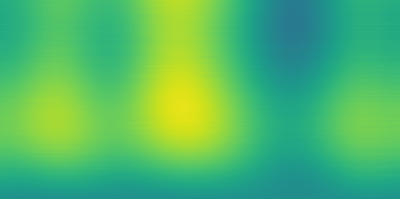
\includegraphics[interpolate=false,width=1.000000in,height=1.000000in]{burgers_exact_diff_0.01-img0.png}}%
\end{pgfscope}%
\begin{pgfscope}%
\pgfsetbuttcap%
\pgfsetroundjoin%
\definecolor{currentfill}{rgb}{0.000000,0.000000,0.000000}%
\pgfsetfillcolor{currentfill}%
\pgfsetlinewidth{0.803000pt}%
\definecolor{currentstroke}{rgb}{0.000000,0.000000,0.000000}%
\pgfsetstrokecolor{currentstroke}%
\pgfsetdash{}{0pt}%
\pgfsys@defobject{currentmarker}{\pgfqpoint{0.000000in}{-0.048611in}}{\pgfqpoint{0.000000in}{0.000000in}}{%
\pgfpathmoveto{\pgfqpoint{0.000000in}{0.000000in}}%
\pgfpathlineto{\pgfqpoint{0.000000in}{-0.048611in}}%
\pgfusepath{stroke,fill}%
}%
\begin{pgfscope}%
\pgfsys@transformshift{0.726837in}{0.517039in}%
\pgfsys@useobject{currentmarker}{}%
\end{pgfscope}%
\end{pgfscope}%
\begin{pgfscope}%
\definecolor{textcolor}{rgb}{0.000000,0.000000,0.000000}%
\pgfsetstrokecolor{textcolor}%
\pgfsetfillcolor{textcolor}%
\pgftext[x=0.726837in,y=0.419816in,,top]{\color{textcolor}\rmfamily\fontsize{12.000000}{14.400000}\selectfont 0}%
\end{pgfscope}%
\begin{pgfscope}%
\pgfsetbuttcap%
\pgfsetroundjoin%
\definecolor{currentfill}{rgb}{0.000000,0.000000,0.000000}%
\pgfsetfillcolor{currentfill}%
\pgfsetlinewidth{0.803000pt}%
\definecolor{currentstroke}{rgb}{0.000000,0.000000,0.000000}%
\pgfsetstrokecolor{currentstroke}%
\pgfsetdash{}{0pt}%
\pgfsys@defobject{currentmarker}{\pgfqpoint{0.000000in}{-0.048611in}}{\pgfqpoint{0.000000in}{0.000000in}}{%
\pgfpathmoveto{\pgfqpoint{0.000000in}{0.000000in}}%
\pgfpathlineto{\pgfqpoint{0.000000in}{-0.048611in}}%
\pgfusepath{stroke,fill}%
}%
\begin{pgfscope}%
\pgfsys@transformshift{1.495229in}{0.517039in}%
\pgfsys@useobject{currentmarker}{}%
\end{pgfscope}%
\end{pgfscope}%
\begin{pgfscope}%
\definecolor{textcolor}{rgb}{0.000000,0.000000,0.000000}%
\pgfsetstrokecolor{textcolor}%
\pgfsetfillcolor{textcolor}%
\pgftext[x=1.495229in,y=0.419816in,,top]{\color{textcolor}\rmfamily\fontsize{12.000000}{14.400000}\selectfont 1}%
\end{pgfscope}%
\begin{pgfscope}%
\pgfsetbuttcap%
\pgfsetroundjoin%
\definecolor{currentfill}{rgb}{0.000000,0.000000,0.000000}%
\pgfsetfillcolor{currentfill}%
\pgfsetlinewidth{0.803000pt}%
\definecolor{currentstroke}{rgb}{0.000000,0.000000,0.000000}%
\pgfsetstrokecolor{currentstroke}%
\pgfsetdash{}{0pt}%
\pgfsys@defobject{currentmarker}{\pgfqpoint{0.000000in}{-0.048611in}}{\pgfqpoint{0.000000in}{0.000000in}}{%
\pgfpathmoveto{\pgfqpoint{0.000000in}{0.000000in}}%
\pgfpathlineto{\pgfqpoint{0.000000in}{-0.048611in}}%
\pgfusepath{stroke,fill}%
}%
\begin{pgfscope}%
\pgfsys@transformshift{2.263621in}{0.517039in}%
\pgfsys@useobject{currentmarker}{}%
\end{pgfscope}%
\end{pgfscope}%
\begin{pgfscope}%
\definecolor{textcolor}{rgb}{0.000000,0.000000,0.000000}%
\pgfsetstrokecolor{textcolor}%
\pgfsetfillcolor{textcolor}%
\pgftext[x=2.263621in,y=0.419816in,,top]{\color{textcolor}\rmfamily\fontsize{12.000000}{14.400000}\selectfont 2}%
\end{pgfscope}%
\begin{pgfscope}%
\definecolor{textcolor}{rgb}{0.000000,0.000000,0.000000}%
\pgfsetstrokecolor{textcolor}%
\pgfsetfillcolor{textcolor}%
\pgftext[x=1.495229in,y=0.202965in,,top]{\color{textcolor}\rmfamily\fontsize{12.000000}{14.400000}\selectfont Space}%
\end{pgfscope}%
\begin{pgfscope}%
\pgfsetbuttcap%
\pgfsetroundjoin%
\definecolor{currentfill}{rgb}{0.000000,0.000000,0.000000}%
\pgfsetfillcolor{currentfill}%
\pgfsetlinewidth{0.803000pt}%
\definecolor{currentstroke}{rgb}{0.000000,0.000000,0.000000}%
\pgfsetstrokecolor{currentstroke}%
\pgfsetdash{}{0pt}%
\pgfsys@defobject{currentmarker}{\pgfqpoint{-0.048611in}{0.000000in}}{\pgfqpoint{-0.000000in}{0.000000in}}{%
\pgfpathmoveto{\pgfqpoint{-0.000000in}{0.000000in}}%
\pgfpathlineto{\pgfqpoint{-0.048611in}{0.000000in}}%
\pgfusepath{stroke,fill}%
}%
\begin{pgfscope}%
\pgfsys@transformshift{0.726837in}{0.517039in}%
\pgfsys@useobject{currentmarker}{}%
\end{pgfscope}%
\end{pgfscope}%
\begin{pgfscope}%
\definecolor{textcolor}{rgb}{0.000000,0.000000,0.000000}%
\pgfsetstrokecolor{textcolor}%
\pgfsetfillcolor{textcolor}%
\pgftext[x=0.364559in, y=0.453725in, left, base]{\color{textcolor}\rmfamily\fontsize{12.000000}{14.400000}\selectfont 0.0}%
\end{pgfscope}%
\begin{pgfscope}%
\pgfsetbuttcap%
\pgfsetroundjoin%
\definecolor{currentfill}{rgb}{0.000000,0.000000,0.000000}%
\pgfsetfillcolor{currentfill}%
\pgfsetlinewidth{0.803000pt}%
\definecolor{currentstroke}{rgb}{0.000000,0.000000,0.000000}%
\pgfsetstrokecolor{currentstroke}%
\pgfsetdash{}{0pt}%
\pgfsys@defobject{currentmarker}{\pgfqpoint{-0.048611in}{0.000000in}}{\pgfqpoint{-0.000000in}{0.000000in}}{%
\pgfpathmoveto{\pgfqpoint{-0.000000in}{0.000000in}}%
\pgfpathlineto{\pgfqpoint{-0.048611in}{0.000000in}}%
\pgfusepath{stroke,fill}%
}%
\begin{pgfscope}%
\pgfsys@transformshift{0.726837in}{0.861533in}%
\pgfsys@useobject{currentmarker}{}%
\end{pgfscope}%
\end{pgfscope}%
\begin{pgfscope}%
\definecolor{textcolor}{rgb}{0.000000,0.000000,0.000000}%
\pgfsetstrokecolor{textcolor}%
\pgfsetfillcolor{textcolor}%
\pgftext[x=0.364559in, y=0.798219in, left, base]{\color{textcolor}\rmfamily\fontsize{12.000000}{14.400000}\selectfont 2.5}%
\end{pgfscope}%
\begin{pgfscope}%
\pgfsetbuttcap%
\pgfsetroundjoin%
\definecolor{currentfill}{rgb}{0.000000,0.000000,0.000000}%
\pgfsetfillcolor{currentfill}%
\pgfsetlinewidth{0.803000pt}%
\definecolor{currentstroke}{rgb}{0.000000,0.000000,0.000000}%
\pgfsetstrokecolor{currentstroke}%
\pgfsetdash{}{0pt}%
\pgfsys@defobject{currentmarker}{\pgfqpoint{-0.048611in}{0.000000in}}{\pgfqpoint{-0.000000in}{0.000000in}}{%
\pgfpathmoveto{\pgfqpoint{-0.000000in}{0.000000in}}%
\pgfpathlineto{\pgfqpoint{-0.048611in}{0.000000in}}%
\pgfusepath{stroke,fill}%
}%
\begin{pgfscope}%
\pgfsys@transformshift{0.726837in}{1.206027in}%
\pgfsys@useobject{currentmarker}{}%
\end{pgfscope}%
\end{pgfscope}%
\begin{pgfscope}%
\definecolor{textcolor}{rgb}{0.000000,0.000000,0.000000}%
\pgfsetstrokecolor{textcolor}%
\pgfsetfillcolor{textcolor}%
\pgftext[x=0.364559in, y=1.142714in, left, base]{\color{textcolor}\rmfamily\fontsize{12.000000}{14.400000}\selectfont 5.0}%
\end{pgfscope}%
\begin{pgfscope}%
\pgfsetbuttcap%
\pgfsetroundjoin%
\definecolor{currentfill}{rgb}{0.000000,0.000000,0.000000}%
\pgfsetfillcolor{currentfill}%
\pgfsetlinewidth{0.803000pt}%
\definecolor{currentstroke}{rgb}{0.000000,0.000000,0.000000}%
\pgfsetstrokecolor{currentstroke}%
\pgfsetdash{}{0pt}%
\pgfsys@defobject{currentmarker}{\pgfqpoint{-0.048611in}{0.000000in}}{\pgfqpoint{-0.000000in}{0.000000in}}{%
\pgfpathmoveto{\pgfqpoint{-0.000000in}{0.000000in}}%
\pgfpathlineto{\pgfqpoint{-0.048611in}{0.000000in}}%
\pgfusepath{stroke,fill}%
}%
\begin{pgfscope}%
\pgfsys@transformshift{0.726837in}{1.550522in}%
\pgfsys@useobject{currentmarker}{}%
\end{pgfscope}%
\end{pgfscope}%
\begin{pgfscope}%
\definecolor{textcolor}{rgb}{0.000000,0.000000,0.000000}%
\pgfsetstrokecolor{textcolor}%
\pgfsetfillcolor{textcolor}%
\pgftext[x=0.364559in, y=1.487208in, left, base]{\color{textcolor}\rmfamily\fontsize{12.000000}{14.400000}\selectfont 7.5}%
\end{pgfscope}%
\begin{pgfscope}%
\pgfsetbuttcap%
\pgfsetroundjoin%
\definecolor{currentfill}{rgb}{0.000000,0.000000,0.000000}%
\pgfsetfillcolor{currentfill}%
\pgfsetlinewidth{0.803000pt}%
\definecolor{currentstroke}{rgb}{0.000000,0.000000,0.000000}%
\pgfsetstrokecolor{currentstroke}%
\pgfsetdash{}{0pt}%
\pgfsys@defobject{currentmarker}{\pgfqpoint{-0.048611in}{0.000000in}}{\pgfqpoint{-0.000000in}{0.000000in}}{%
\pgfpathmoveto{\pgfqpoint{-0.000000in}{0.000000in}}%
\pgfpathlineto{\pgfqpoint{-0.048611in}{0.000000in}}%
\pgfusepath{stroke,fill}%
}%
\begin{pgfscope}%
\pgfsys@transformshift{0.726837in}{1.895016in}%
\pgfsys@useobject{currentmarker}{}%
\end{pgfscope}%
\end{pgfscope}%
\begin{pgfscope}%
\definecolor{textcolor}{rgb}{0.000000,0.000000,0.000000}%
\pgfsetstrokecolor{textcolor}%
\pgfsetfillcolor{textcolor}%
\pgftext[x=0.258521in, y=1.831702in, left, base]{\color{textcolor}\rmfamily\fontsize{12.000000}{14.400000}\selectfont 10.0}%
\end{pgfscope}%
\begin{pgfscope}%
\definecolor{textcolor}{rgb}{0.000000,0.000000,0.000000}%
\pgfsetstrokecolor{textcolor}%
\pgfsetfillcolor{textcolor}%
\pgftext[x=0.202965in,y=1.206027in,,bottom,rotate=90.000000]{\color{textcolor}\rmfamily\fontsize{12.000000}{14.400000}\selectfont Time}%
\end{pgfscope}%
\begin{pgfscope}%
\pgfsetrectcap%
\pgfsetmiterjoin%
\pgfsetlinewidth{0.803000pt}%
\definecolor{currentstroke}{rgb}{0.000000,0.000000,0.000000}%
\pgfsetstrokecolor{currentstroke}%
\pgfsetdash{}{0pt}%
\pgfpathmoveto{\pgfqpoint{0.726837in}{0.517039in}}%
\pgfpathlineto{\pgfqpoint{0.726837in}{1.895016in}}%
\pgfusepath{stroke}%
\end{pgfscope}%
\begin{pgfscope}%
\pgfsetrectcap%
\pgfsetmiterjoin%
\pgfsetlinewidth{0.803000pt}%
\definecolor{currentstroke}{rgb}{0.000000,0.000000,0.000000}%
\pgfsetstrokecolor{currentstroke}%
\pgfsetdash{}{0pt}%
\pgfpathmoveto{\pgfqpoint{2.263621in}{0.517039in}}%
\pgfpathlineto{\pgfqpoint{2.263621in}{1.895016in}}%
\pgfusepath{stroke}%
\end{pgfscope}%
\begin{pgfscope}%
\pgfsetrectcap%
\pgfsetmiterjoin%
\pgfsetlinewidth{0.803000pt}%
\definecolor{currentstroke}{rgb}{0.000000,0.000000,0.000000}%
\pgfsetstrokecolor{currentstroke}%
\pgfsetdash{}{0pt}%
\pgfpathmoveto{\pgfqpoint{0.726837in}{0.517039in}}%
\pgfpathlineto{\pgfqpoint{2.263621in}{0.517039in}}%
\pgfusepath{stroke}%
\end{pgfscope}%
\begin{pgfscope}%
\pgfsetrectcap%
\pgfsetmiterjoin%
\pgfsetlinewidth{0.803000pt}%
\definecolor{currentstroke}{rgb}{0.000000,0.000000,0.000000}%
\pgfsetstrokecolor{currentstroke}%
\pgfsetdash{}{0pt}%
\pgfpathmoveto{\pgfqpoint{0.726837in}{1.895016in}}%
\pgfpathlineto{\pgfqpoint{2.263621in}{1.895016in}}%
\pgfusepath{stroke}%
\end{pgfscope}%
\begin{pgfscope}%
\pgfsetbuttcap%
\pgfsetmiterjoin%
\pgfsetlinewidth{0.000000pt}%
\definecolor{currentstroke}{rgb}{0.000000,0.000000,0.000000}%
\pgfsetstrokecolor{currentstroke}%
\pgfsetstrokeopacity{0.000000}%
\pgfsetdash{}{0pt}%
\pgfpathmoveto{\pgfqpoint{2.393479in}{0.517039in}}%
\pgfpathlineto{\pgfqpoint{2.462378in}{0.517039in}}%
\pgfpathlineto{\pgfqpoint{2.462378in}{1.895016in}}%
\pgfpathlineto{\pgfqpoint{2.393479in}{1.895016in}}%
\pgfpathlineto{\pgfqpoint{2.393479in}{0.517039in}}%
\pgfpathclose%
\pgfusepath{}%
\end{pgfscope}%
\begin{pgfscope}%
\pgfsys@transformshift{2.390000in}{0.520000in}%
\pgftext[left,bottom]{
\includegraphics[interpolate=true,width=0.070000in,height=1.380000in]{burgers_exact_diff_0.01-img1.png}}%
\end{pgfscope}%
\begin{pgfscope}%
\pgfsetbuttcap%
\pgfsetroundjoin%
\definecolor{currentfill}{rgb}{0.000000,0.000000,0.000000}%
\pgfsetfillcolor{currentfill}%
\pgfsetlinewidth{0.803000pt}%
\definecolor{currentstroke}{rgb}{0.000000,0.000000,0.000000}%
\pgfsetstrokecolor{currentstroke}%
\pgfsetdash{}{0pt}%
\pgfsys@defobject{currentmarker}{\pgfqpoint{0.000000in}{0.000000in}}{\pgfqpoint{0.048611in}{0.000000in}}{%
\pgfpathmoveto{\pgfqpoint{0.000000in}{0.000000in}}%
\pgfpathlineto{\pgfqpoint{0.048611in}{0.000000in}}%
\pgfusepath{stroke,fill}%
}%
\begin{pgfscope}%
\pgfsys@transformshift{2.462378in}{0.649681in}%
\pgfsys@useobject{currentmarker}{}%
\end{pgfscope}%
\end{pgfscope}%
\begin{pgfscope}%
\definecolor{textcolor}{rgb}{0.000000,0.000000,0.000000}%
\pgfsetstrokecolor{textcolor}%
\pgfsetfillcolor{textcolor}%
\pgftext[x=2.559601in, y=0.586367in, left, base]{\color{textcolor}\rmfamily\fontsize{12.000000}{14.400000}\selectfont \ensuremath{-}0.1}%
\end{pgfscope}%
\begin{pgfscope}%
\pgfsetbuttcap%
\pgfsetroundjoin%
\definecolor{currentfill}{rgb}{0.000000,0.000000,0.000000}%
\pgfsetfillcolor{currentfill}%
\pgfsetlinewidth{0.803000pt}%
\definecolor{currentstroke}{rgb}{0.000000,0.000000,0.000000}%
\pgfsetstrokecolor{currentstroke}%
\pgfsetdash{}{0pt}%
\pgfsys@defobject{currentmarker}{\pgfqpoint{0.000000in}{0.000000in}}{\pgfqpoint{0.048611in}{0.000000in}}{%
\pgfpathmoveto{\pgfqpoint{0.000000in}{0.000000in}}%
\pgfpathlineto{\pgfqpoint{0.048611in}{0.000000in}}%
\pgfusepath{stroke,fill}%
}%
\begin{pgfscope}%
\pgfsys@transformshift{2.462378in}{1.206027in}%
\pgfsys@useobject{currentmarker}{}%
\end{pgfscope}%
\end{pgfscope}%
\begin{pgfscope}%
\definecolor{textcolor}{rgb}{0.000000,0.000000,0.000000}%
\pgfsetstrokecolor{textcolor}%
\pgfsetfillcolor{textcolor}%
\pgftext[x=2.559601in, y=1.142714in, left, base]{\color{textcolor}\rmfamily\fontsize{12.000000}{14.400000}\selectfont 0.0}%
\end{pgfscope}%
\begin{pgfscope}%
\pgfsetbuttcap%
\pgfsetroundjoin%
\definecolor{currentfill}{rgb}{0.000000,0.000000,0.000000}%
\pgfsetfillcolor{currentfill}%
\pgfsetlinewidth{0.803000pt}%
\definecolor{currentstroke}{rgb}{0.000000,0.000000,0.000000}%
\pgfsetstrokecolor{currentstroke}%
\pgfsetdash{}{0pt}%
\pgfsys@defobject{currentmarker}{\pgfqpoint{0.000000in}{0.000000in}}{\pgfqpoint{0.048611in}{0.000000in}}{%
\pgfpathmoveto{\pgfqpoint{0.000000in}{0.000000in}}%
\pgfpathlineto{\pgfqpoint{0.048611in}{0.000000in}}%
\pgfusepath{stroke,fill}%
}%
\begin{pgfscope}%
\pgfsys@transformshift{2.462378in}{1.762374in}%
\pgfsys@useobject{currentmarker}{}%
\end{pgfscope}%
\end{pgfscope}%
\begin{pgfscope}%
\definecolor{textcolor}{rgb}{0.000000,0.000000,0.000000}%
\pgfsetstrokecolor{textcolor}%
\pgfsetfillcolor{textcolor}%
\pgftext[x=2.559601in, y=1.699060in, left, base]{\color{textcolor}\rmfamily\fontsize{12.000000}{14.400000}\selectfont 0.1}%
\end{pgfscope}%
\begin{pgfscope}%
\pgfsetrectcap%
\pgfsetmiterjoin%
\pgfsetlinewidth{0.803000pt}%
\definecolor{currentstroke}{rgb}{0.000000,0.000000,0.000000}%
\pgfsetstrokecolor{currentstroke}%
\pgfsetdash{}{0pt}%
\pgfpathmoveto{\pgfqpoint{2.393479in}{0.517039in}}%
\pgfpathlineto{\pgfqpoint{2.427929in}{0.517039in}}%
\pgfpathlineto{\pgfqpoint{2.462378in}{0.517039in}}%
\pgfpathlineto{\pgfqpoint{2.462378in}{1.895016in}}%
\pgfpathlineto{\pgfqpoint{2.427929in}{1.895016in}}%
\pgfpathlineto{\pgfqpoint{2.393479in}{1.895016in}}%
\pgfpathlineto{\pgfqpoint{2.393479in}{0.517039in}}%
\pgfpathclose%
\pgfusepath{stroke}%
\end{pgfscope}%
\end{pgfpicture}%
\makeatother%
\endgroup%

      \end{adjustbox}
      \caption{The difference for \(\nu=0.01\)}\label{fig:sc2_exact_diff_0.01}
    \end{subfigure}
    \\[0.7\baselineskip]
    \begin{subfigure}{0.33\linewidth}
      \begin{adjustbox}{width=\linewidth}
        \begingroup%
\makeatletter%
\begin{pgfpicture}%
\pgfpathrectangle{\pgfpointorigin}{\pgfqpoint{3.000000in}{2.000000in}}%
\pgfusepath{use as bounding box, clip}%
\begin{pgfscope}%
\pgfsetbuttcap%
\pgfsetmiterjoin%
\pgfsetlinewidth{0.000000pt}%
\definecolor{currentstroke}{rgb}{0.000000,0.000000,0.000000}%
\pgfsetstrokecolor{currentstroke}%
\pgfsetstrokeopacity{0.000000}%
\pgfsetdash{}{0pt}%
\pgfpathmoveto{\pgfqpoint{0.000000in}{0.000000in}}%
\pgfpathlineto{\pgfqpoint{3.000000in}{0.000000in}}%
\pgfpathlineto{\pgfqpoint{3.000000in}{2.000000in}}%
\pgfpathlineto{\pgfqpoint{0.000000in}{2.000000in}}%
\pgfpathlineto{\pgfqpoint{0.000000in}{0.000000in}}%
\pgfpathclose%
\pgfusepath{}%
\end{pgfscope}%
\begin{pgfscope}%
\pgfsetbuttcap%
\pgfsetmiterjoin%
\pgfsetlinewidth{0.000000pt}%
\definecolor{currentstroke}{rgb}{0.000000,0.000000,0.000000}%
\pgfsetstrokecolor{currentstroke}%
\pgfsetstrokeopacity{0.000000}%
\pgfsetdash{}{0pt}%
\pgfpathmoveto{\pgfqpoint{0.726837in}{0.517039in}}%
\pgfpathlineto{\pgfqpoint{2.263621in}{0.517039in}}%
\pgfpathlineto{\pgfqpoint{2.263621in}{1.895016in}}%
\pgfpathlineto{\pgfqpoint{0.726837in}{1.895016in}}%
\pgfpathlineto{\pgfqpoint{0.726837in}{0.517039in}}%
\pgfpathclose%
\pgfusepath{}%
\end{pgfscope}%
\begin{pgfscope}%
\pgfpathrectangle{\pgfqpoint{0.726837in}{0.517039in}}{\pgfqpoint{1.536784in}{1.377978in}}%
\pgfusepath{clip}%
\pgfsys@transformcm{1.536784}{0.000000}{0.000000}{1.377978}{0.726837in}{0.517039in}%
\pgftext[left,bottom]{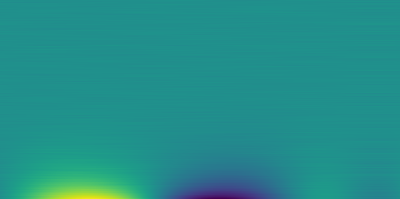
\includegraphics[interpolate=false,width=1.000000in,height=1.000000in]{burgers_exact_target_0.1-img0.png}}%
\end{pgfscope}%
\begin{pgfscope}%
\pgfsetbuttcap%
\pgfsetroundjoin%
\definecolor{currentfill}{rgb}{0.000000,0.000000,0.000000}%
\pgfsetfillcolor{currentfill}%
\pgfsetlinewidth{0.803000pt}%
\definecolor{currentstroke}{rgb}{0.000000,0.000000,0.000000}%
\pgfsetstrokecolor{currentstroke}%
\pgfsetdash{}{0pt}%
\pgfsys@defobject{currentmarker}{\pgfqpoint{0.000000in}{-0.048611in}}{\pgfqpoint{0.000000in}{0.000000in}}{%
\pgfpathmoveto{\pgfqpoint{0.000000in}{0.000000in}}%
\pgfpathlineto{\pgfqpoint{0.000000in}{-0.048611in}}%
\pgfusepath{stroke,fill}%
}%
\begin{pgfscope}%
\pgfsys@transformshift{0.726837in}{0.517039in}%
\pgfsys@useobject{currentmarker}{}%
\end{pgfscope}%
\end{pgfscope}%
\begin{pgfscope}%
\definecolor{textcolor}{rgb}{0.000000,0.000000,0.000000}%
\pgfsetstrokecolor{textcolor}%
\pgfsetfillcolor{textcolor}%
\pgftext[x=0.726837in,y=0.419816in,,top]{\color{textcolor}{\rmfamily\fontsize{12.000000}{14.400000}\selectfont\catcode`\^=\active\def^{\ifmmode\sp\else\^{}\fi}\catcode`\%=\active\def%{\%}0}}%
\end{pgfscope}%
\begin{pgfscope}%
\pgfsetbuttcap%
\pgfsetroundjoin%
\definecolor{currentfill}{rgb}{0.000000,0.000000,0.000000}%
\pgfsetfillcolor{currentfill}%
\pgfsetlinewidth{0.803000pt}%
\definecolor{currentstroke}{rgb}{0.000000,0.000000,0.000000}%
\pgfsetstrokecolor{currentstroke}%
\pgfsetdash{}{0pt}%
\pgfsys@defobject{currentmarker}{\pgfqpoint{0.000000in}{-0.048611in}}{\pgfqpoint{0.000000in}{0.000000in}}{%
\pgfpathmoveto{\pgfqpoint{0.000000in}{0.000000in}}%
\pgfpathlineto{\pgfqpoint{0.000000in}{-0.048611in}}%
\pgfusepath{stroke,fill}%
}%
\begin{pgfscope}%
\pgfsys@transformshift{1.495229in}{0.517039in}%
\pgfsys@useobject{currentmarker}{}%
\end{pgfscope}%
\end{pgfscope}%
\begin{pgfscope}%
\definecolor{textcolor}{rgb}{0.000000,0.000000,0.000000}%
\pgfsetstrokecolor{textcolor}%
\pgfsetfillcolor{textcolor}%
\pgftext[x=1.495229in,y=0.419816in,,top]{\color{textcolor}{\rmfamily\fontsize{12.000000}{14.400000}\selectfont\catcode`\^=\active\def^{\ifmmode\sp\else\^{}\fi}\catcode`\%=\active\def%{\%}1}}%
\end{pgfscope}%
\begin{pgfscope}%
\pgfsetbuttcap%
\pgfsetroundjoin%
\definecolor{currentfill}{rgb}{0.000000,0.000000,0.000000}%
\pgfsetfillcolor{currentfill}%
\pgfsetlinewidth{0.803000pt}%
\definecolor{currentstroke}{rgb}{0.000000,0.000000,0.000000}%
\pgfsetstrokecolor{currentstroke}%
\pgfsetdash{}{0pt}%
\pgfsys@defobject{currentmarker}{\pgfqpoint{0.000000in}{-0.048611in}}{\pgfqpoint{0.000000in}{0.000000in}}{%
\pgfpathmoveto{\pgfqpoint{0.000000in}{0.000000in}}%
\pgfpathlineto{\pgfqpoint{0.000000in}{-0.048611in}}%
\pgfusepath{stroke,fill}%
}%
\begin{pgfscope}%
\pgfsys@transformshift{2.263621in}{0.517039in}%
\pgfsys@useobject{currentmarker}{}%
\end{pgfscope}%
\end{pgfscope}%
\begin{pgfscope}%
\definecolor{textcolor}{rgb}{0.000000,0.000000,0.000000}%
\pgfsetstrokecolor{textcolor}%
\pgfsetfillcolor{textcolor}%
\pgftext[x=2.263621in,y=0.419816in,,top]{\color{textcolor}{\rmfamily\fontsize{12.000000}{14.400000}\selectfont\catcode`\^=\active\def^{\ifmmode\sp\else\^{}\fi}\catcode`\%=\active\def%{\%}2}}%
\end{pgfscope}%
\begin{pgfscope}%
\definecolor{textcolor}{rgb}{0.000000,0.000000,0.000000}%
\pgfsetstrokecolor{textcolor}%
\pgfsetfillcolor{textcolor}%
\pgftext[x=1.495229in,y=0.202965in,,top]{\color{textcolor}{\rmfamily\fontsize{12.000000}{14.400000}\selectfont\catcode`\^=\active\def^{\ifmmode\sp\else\^{}\fi}\catcode`\%=\active\def%{\%}Space}}%
\end{pgfscope}%
\begin{pgfscope}%
\pgfsetbuttcap%
\pgfsetroundjoin%
\definecolor{currentfill}{rgb}{0.000000,0.000000,0.000000}%
\pgfsetfillcolor{currentfill}%
\pgfsetlinewidth{0.803000pt}%
\definecolor{currentstroke}{rgb}{0.000000,0.000000,0.000000}%
\pgfsetstrokecolor{currentstroke}%
\pgfsetdash{}{0pt}%
\pgfsys@defobject{currentmarker}{\pgfqpoint{-0.048611in}{0.000000in}}{\pgfqpoint{-0.000000in}{0.000000in}}{%
\pgfpathmoveto{\pgfqpoint{-0.000000in}{0.000000in}}%
\pgfpathlineto{\pgfqpoint{-0.048611in}{0.000000in}}%
\pgfusepath{stroke,fill}%
}%
\begin{pgfscope}%
\pgfsys@transformshift{0.726837in}{0.517039in}%
\pgfsys@useobject{currentmarker}{}%
\end{pgfscope}%
\end{pgfscope}%
\begin{pgfscope}%
\definecolor{textcolor}{rgb}{0.000000,0.000000,0.000000}%
\pgfsetstrokecolor{textcolor}%
\pgfsetfillcolor{textcolor}%
\pgftext[x=0.364559in, y=0.453725in, left, base]{\color{textcolor}{\rmfamily\fontsize{12.000000}{14.400000}\selectfont\catcode`\^=\active\def^{\ifmmode\sp\else\^{}\fi}\catcode`\%=\active\def%{\%}0.0}}%
\end{pgfscope}%
\begin{pgfscope}%
\pgfsetbuttcap%
\pgfsetroundjoin%
\definecolor{currentfill}{rgb}{0.000000,0.000000,0.000000}%
\pgfsetfillcolor{currentfill}%
\pgfsetlinewidth{0.803000pt}%
\definecolor{currentstroke}{rgb}{0.000000,0.000000,0.000000}%
\pgfsetstrokecolor{currentstroke}%
\pgfsetdash{}{0pt}%
\pgfsys@defobject{currentmarker}{\pgfqpoint{-0.048611in}{0.000000in}}{\pgfqpoint{-0.000000in}{0.000000in}}{%
\pgfpathmoveto{\pgfqpoint{-0.000000in}{0.000000in}}%
\pgfpathlineto{\pgfqpoint{-0.048611in}{0.000000in}}%
\pgfusepath{stroke,fill}%
}%
\begin{pgfscope}%
\pgfsys@transformshift{0.726837in}{0.861533in}%
\pgfsys@useobject{currentmarker}{}%
\end{pgfscope}%
\end{pgfscope}%
\begin{pgfscope}%
\definecolor{textcolor}{rgb}{0.000000,0.000000,0.000000}%
\pgfsetstrokecolor{textcolor}%
\pgfsetfillcolor{textcolor}%
\pgftext[x=0.364559in, y=0.798219in, left, base]{\color{textcolor}{\rmfamily\fontsize{12.000000}{14.400000}\selectfont\catcode`\^=\active\def^{\ifmmode\sp\else\^{}\fi}\catcode`\%=\active\def%{\%}2.5}}%
\end{pgfscope}%
\begin{pgfscope}%
\pgfsetbuttcap%
\pgfsetroundjoin%
\definecolor{currentfill}{rgb}{0.000000,0.000000,0.000000}%
\pgfsetfillcolor{currentfill}%
\pgfsetlinewidth{0.803000pt}%
\definecolor{currentstroke}{rgb}{0.000000,0.000000,0.000000}%
\pgfsetstrokecolor{currentstroke}%
\pgfsetdash{}{0pt}%
\pgfsys@defobject{currentmarker}{\pgfqpoint{-0.048611in}{0.000000in}}{\pgfqpoint{-0.000000in}{0.000000in}}{%
\pgfpathmoveto{\pgfqpoint{-0.000000in}{0.000000in}}%
\pgfpathlineto{\pgfqpoint{-0.048611in}{0.000000in}}%
\pgfusepath{stroke,fill}%
}%
\begin{pgfscope}%
\pgfsys@transformshift{0.726837in}{1.206027in}%
\pgfsys@useobject{currentmarker}{}%
\end{pgfscope}%
\end{pgfscope}%
\begin{pgfscope}%
\definecolor{textcolor}{rgb}{0.000000,0.000000,0.000000}%
\pgfsetstrokecolor{textcolor}%
\pgfsetfillcolor{textcolor}%
\pgftext[x=0.364559in, y=1.142714in, left, base]{\color{textcolor}{\rmfamily\fontsize{12.000000}{14.400000}\selectfont\catcode`\^=\active\def^{\ifmmode\sp\else\^{}\fi}\catcode`\%=\active\def%{\%}5.0}}%
\end{pgfscope}%
\begin{pgfscope}%
\pgfsetbuttcap%
\pgfsetroundjoin%
\definecolor{currentfill}{rgb}{0.000000,0.000000,0.000000}%
\pgfsetfillcolor{currentfill}%
\pgfsetlinewidth{0.803000pt}%
\definecolor{currentstroke}{rgb}{0.000000,0.000000,0.000000}%
\pgfsetstrokecolor{currentstroke}%
\pgfsetdash{}{0pt}%
\pgfsys@defobject{currentmarker}{\pgfqpoint{-0.048611in}{0.000000in}}{\pgfqpoint{-0.000000in}{0.000000in}}{%
\pgfpathmoveto{\pgfqpoint{-0.000000in}{0.000000in}}%
\pgfpathlineto{\pgfqpoint{-0.048611in}{0.000000in}}%
\pgfusepath{stroke,fill}%
}%
\begin{pgfscope}%
\pgfsys@transformshift{0.726837in}{1.550522in}%
\pgfsys@useobject{currentmarker}{}%
\end{pgfscope}%
\end{pgfscope}%
\begin{pgfscope}%
\definecolor{textcolor}{rgb}{0.000000,0.000000,0.000000}%
\pgfsetstrokecolor{textcolor}%
\pgfsetfillcolor{textcolor}%
\pgftext[x=0.364559in, y=1.487208in, left, base]{\color{textcolor}{\rmfamily\fontsize{12.000000}{14.400000}\selectfont\catcode`\^=\active\def^{\ifmmode\sp\else\^{}\fi}\catcode`\%=\active\def%{\%}7.5}}%
\end{pgfscope}%
\begin{pgfscope}%
\pgfsetbuttcap%
\pgfsetroundjoin%
\definecolor{currentfill}{rgb}{0.000000,0.000000,0.000000}%
\pgfsetfillcolor{currentfill}%
\pgfsetlinewidth{0.803000pt}%
\definecolor{currentstroke}{rgb}{0.000000,0.000000,0.000000}%
\pgfsetstrokecolor{currentstroke}%
\pgfsetdash{}{0pt}%
\pgfsys@defobject{currentmarker}{\pgfqpoint{-0.048611in}{0.000000in}}{\pgfqpoint{-0.000000in}{0.000000in}}{%
\pgfpathmoveto{\pgfqpoint{-0.000000in}{0.000000in}}%
\pgfpathlineto{\pgfqpoint{-0.048611in}{0.000000in}}%
\pgfusepath{stroke,fill}%
}%
\begin{pgfscope}%
\pgfsys@transformshift{0.726837in}{1.895016in}%
\pgfsys@useobject{currentmarker}{}%
\end{pgfscope}%
\end{pgfscope}%
\begin{pgfscope}%
\definecolor{textcolor}{rgb}{0.000000,0.000000,0.000000}%
\pgfsetstrokecolor{textcolor}%
\pgfsetfillcolor{textcolor}%
\pgftext[x=0.258521in, y=1.831702in, left, base]{\color{textcolor}{\rmfamily\fontsize{12.000000}{14.400000}\selectfont\catcode`\^=\active\def^{\ifmmode\sp\else\^{}\fi}\catcode`\%=\active\def%{\%}10.0}}%
\end{pgfscope}%
\begin{pgfscope}%
\definecolor{textcolor}{rgb}{0.000000,0.000000,0.000000}%
\pgfsetstrokecolor{textcolor}%
\pgfsetfillcolor{textcolor}%
\pgftext[x=0.202965in,y=1.206027in,,bottom,rotate=90.000000]{\color{textcolor}{\rmfamily\fontsize{12.000000}{14.400000}\selectfont\catcode`\^=\active\def^{\ifmmode\sp\else\^{}\fi}\catcode`\%=\active\def%{\%}Time}}%
\end{pgfscope}%
\begin{pgfscope}%
\pgfsetrectcap%
\pgfsetmiterjoin%
\pgfsetlinewidth{0.803000pt}%
\definecolor{currentstroke}{rgb}{0.000000,0.000000,0.000000}%
\pgfsetstrokecolor{currentstroke}%
\pgfsetdash{}{0pt}%
\pgfpathmoveto{\pgfqpoint{0.726837in}{0.517039in}}%
\pgfpathlineto{\pgfqpoint{0.726837in}{1.895016in}}%
\pgfusepath{stroke}%
\end{pgfscope}%
\begin{pgfscope}%
\pgfsetrectcap%
\pgfsetmiterjoin%
\pgfsetlinewidth{0.803000pt}%
\definecolor{currentstroke}{rgb}{0.000000,0.000000,0.000000}%
\pgfsetstrokecolor{currentstroke}%
\pgfsetdash{}{0pt}%
\pgfpathmoveto{\pgfqpoint{2.263621in}{0.517039in}}%
\pgfpathlineto{\pgfqpoint{2.263621in}{1.895016in}}%
\pgfusepath{stroke}%
\end{pgfscope}%
\begin{pgfscope}%
\pgfsetrectcap%
\pgfsetmiterjoin%
\pgfsetlinewidth{0.803000pt}%
\definecolor{currentstroke}{rgb}{0.000000,0.000000,0.000000}%
\pgfsetstrokecolor{currentstroke}%
\pgfsetdash{}{0pt}%
\pgfpathmoveto{\pgfqpoint{0.726837in}{0.517039in}}%
\pgfpathlineto{\pgfqpoint{2.263621in}{0.517039in}}%
\pgfusepath{stroke}%
\end{pgfscope}%
\begin{pgfscope}%
\pgfsetrectcap%
\pgfsetmiterjoin%
\pgfsetlinewidth{0.803000pt}%
\definecolor{currentstroke}{rgb}{0.000000,0.000000,0.000000}%
\pgfsetstrokecolor{currentstroke}%
\pgfsetdash{}{0pt}%
\pgfpathmoveto{\pgfqpoint{0.726837in}{1.895016in}}%
\pgfpathlineto{\pgfqpoint{2.263621in}{1.895016in}}%
\pgfusepath{stroke}%
\end{pgfscope}%
\begin{pgfscope}%
\pgfsetbuttcap%
\pgfsetmiterjoin%
\pgfsetlinewidth{0.000000pt}%
\definecolor{currentstroke}{rgb}{0.000000,0.000000,0.000000}%
\pgfsetstrokecolor{currentstroke}%
\pgfsetstrokeopacity{0.000000}%
\pgfsetdash{}{0pt}%
\pgfpathmoveto{\pgfqpoint{2.393479in}{0.517039in}}%
\pgfpathlineto{\pgfqpoint{2.462378in}{0.517039in}}%
\pgfpathlineto{\pgfqpoint{2.462378in}{1.895016in}}%
\pgfpathlineto{\pgfqpoint{2.393479in}{1.895016in}}%
\pgfpathlineto{\pgfqpoint{2.393479in}{0.517039in}}%
\pgfpathclose%
\pgfusepath{}%
\end{pgfscope}%
\begin{pgfscope}%
\pgfsys@transformshift{2.390000in}{0.520000in}%
\pgftext[left,bottom]{
\includegraphics[interpolate=true,width=0.070000in,height=1.380000in]{burgers_exact_target_0.1-img1.png}}%
\end{pgfscope}%
\begin{pgfscope}%
\pgfsetbuttcap%
\pgfsetroundjoin%
\definecolor{currentfill}{rgb}{0.000000,0.000000,0.000000}%
\pgfsetfillcolor{currentfill}%
\pgfsetlinewidth{0.803000pt}%
\definecolor{currentstroke}{rgb}{0.000000,0.000000,0.000000}%
\pgfsetstrokecolor{currentstroke}%
\pgfsetdash{}{0pt}%
\pgfsys@defobject{currentmarker}{\pgfqpoint{0.000000in}{0.000000in}}{\pgfqpoint{0.048611in}{0.000000in}}{%
\pgfpathmoveto{\pgfqpoint{0.000000in}{0.000000in}}%
\pgfpathlineto{\pgfqpoint{0.048611in}{0.000000in}}%
\pgfusepath{stroke,fill}%
}%
\begin{pgfscope}%
\pgfsys@transformshift{2.462378in}{0.572980in}%
\pgfsys@useobject{currentmarker}{}%
\end{pgfscope}%
\end{pgfscope}%
\begin{pgfscope}%
\definecolor{textcolor}{rgb}{0.000000,0.000000,0.000000}%
\pgfsetstrokecolor{textcolor}%
\pgfsetfillcolor{textcolor}%
\pgftext[x=2.559601in, y=0.509667in, left, base]{\color{textcolor}{\rmfamily\fontsize{12.000000}{14.400000}\selectfont\catcode`\^=\active\def^{\ifmmode\sp\else\^{}\fi}\catcode`\%=\active\def%{\%}\ensuremath{-}0.2}}%
\end{pgfscope}%
\begin{pgfscope}%
\pgfsetbuttcap%
\pgfsetroundjoin%
\definecolor{currentfill}{rgb}{0.000000,0.000000,0.000000}%
\pgfsetfillcolor{currentfill}%
\pgfsetlinewidth{0.803000pt}%
\definecolor{currentstroke}{rgb}{0.000000,0.000000,0.000000}%
\pgfsetstrokecolor{currentstroke}%
\pgfsetdash{}{0pt}%
\pgfsys@defobject{currentmarker}{\pgfqpoint{0.000000in}{0.000000in}}{\pgfqpoint{0.048611in}{0.000000in}}{%
\pgfpathmoveto{\pgfqpoint{0.000000in}{0.000000in}}%
\pgfpathlineto{\pgfqpoint{0.048611in}{0.000000in}}%
\pgfusepath{stroke,fill}%
}%
\begin{pgfscope}%
\pgfsys@transformshift{2.462378in}{1.206027in}%
\pgfsys@useobject{currentmarker}{}%
\end{pgfscope}%
\end{pgfscope}%
\begin{pgfscope}%
\definecolor{textcolor}{rgb}{0.000000,0.000000,0.000000}%
\pgfsetstrokecolor{textcolor}%
\pgfsetfillcolor{textcolor}%
\pgftext[x=2.559601in, y=1.142714in, left, base]{\color{textcolor}{\rmfamily\fontsize{12.000000}{14.400000}\selectfont\catcode`\^=\active\def^{\ifmmode\sp\else\^{}\fi}\catcode`\%=\active\def%{\%}0.0}}%
\end{pgfscope}%
\begin{pgfscope}%
\pgfsetbuttcap%
\pgfsetroundjoin%
\definecolor{currentfill}{rgb}{0.000000,0.000000,0.000000}%
\pgfsetfillcolor{currentfill}%
\pgfsetlinewidth{0.803000pt}%
\definecolor{currentstroke}{rgb}{0.000000,0.000000,0.000000}%
\pgfsetstrokecolor{currentstroke}%
\pgfsetdash{}{0pt}%
\pgfsys@defobject{currentmarker}{\pgfqpoint{0.000000in}{0.000000in}}{\pgfqpoint{0.048611in}{0.000000in}}{%
\pgfpathmoveto{\pgfqpoint{0.000000in}{0.000000in}}%
\pgfpathlineto{\pgfqpoint{0.048611in}{0.000000in}}%
\pgfusepath{stroke,fill}%
}%
\begin{pgfscope}%
\pgfsys@transformshift{2.462378in}{1.839074in}%
\pgfsys@useobject{currentmarker}{}%
\end{pgfscope}%
\end{pgfscope}%
\begin{pgfscope}%
\definecolor{textcolor}{rgb}{0.000000,0.000000,0.000000}%
\pgfsetstrokecolor{textcolor}%
\pgfsetfillcolor{textcolor}%
\pgftext[x=2.559601in, y=1.775761in, left, base]{\color{textcolor}{\rmfamily\fontsize{12.000000}{14.400000}\selectfont\catcode`\^=\active\def^{\ifmmode\sp\else\^{}\fi}\catcode`\%=\active\def%{\%}0.2}}%
\end{pgfscope}%
\begin{pgfscope}%
\pgfsetrectcap%
\pgfsetmiterjoin%
\pgfsetlinewidth{0.803000pt}%
\definecolor{currentstroke}{rgb}{0.000000,0.000000,0.000000}%
\pgfsetstrokecolor{currentstroke}%
\pgfsetdash{}{0pt}%
\pgfpathmoveto{\pgfqpoint{2.393479in}{0.517039in}}%
\pgfpathlineto{\pgfqpoint{2.427929in}{0.517039in}}%
\pgfpathlineto{\pgfqpoint{2.462378in}{0.517039in}}%
\pgfpathlineto{\pgfqpoint{2.462378in}{1.895016in}}%
\pgfpathlineto{\pgfqpoint{2.427929in}{1.895016in}}%
\pgfpathlineto{\pgfqpoint{2.393479in}{1.895016in}}%
\pgfpathlineto{\pgfqpoint{2.393479in}{0.517039in}}%
\pgfpathclose%
\pgfusepath{stroke}%
\end{pgfscope}%
\end{pgfpicture}%
\makeatother%
\endgroup%

      \end{adjustbox}
      \caption{The target for \(\nu=0.1\)}\label{fig:sc2_exact_target_0.1}
    \end{subfigure}
    \begin{subfigure}{0.33\linewidth}
      \begin{adjustbox}{width=\linewidth}
        \begingroup%
\makeatletter%
\begin{pgfpicture}%
\pgfpathrectangle{\pgfpointorigin}{\pgfqpoint{3.000000in}{2.000000in}}%
\pgfusepath{use as bounding box, clip}%
\begin{pgfscope}%
\pgfsetbuttcap%
\pgfsetmiterjoin%
\pgfsetlinewidth{0.000000pt}%
\definecolor{currentstroke}{rgb}{0.000000,0.000000,0.000000}%
\pgfsetstrokecolor{currentstroke}%
\pgfsetstrokeopacity{0.000000}%
\pgfsetdash{}{0pt}%
\pgfpathmoveto{\pgfqpoint{0.000000in}{0.000000in}}%
\pgfpathlineto{\pgfqpoint{3.000000in}{0.000000in}}%
\pgfpathlineto{\pgfqpoint{3.000000in}{2.000000in}}%
\pgfpathlineto{\pgfqpoint{0.000000in}{2.000000in}}%
\pgfpathlineto{\pgfqpoint{0.000000in}{0.000000in}}%
\pgfpathclose%
\pgfusepath{}%
\end{pgfscope}%
\begin{pgfscope}%
\pgfsetbuttcap%
\pgfsetmiterjoin%
\pgfsetlinewidth{0.000000pt}%
\definecolor{currentstroke}{rgb}{0.000000,0.000000,0.000000}%
\pgfsetstrokecolor{currentstroke}%
\pgfsetstrokeopacity{0.000000}%
\pgfsetdash{}{0pt}%
\pgfpathmoveto{\pgfqpoint{0.726837in}{0.517039in}}%
\pgfpathlineto{\pgfqpoint{2.263621in}{0.517039in}}%
\pgfpathlineto{\pgfqpoint{2.263621in}{1.895016in}}%
\pgfpathlineto{\pgfqpoint{0.726837in}{1.895016in}}%
\pgfpathlineto{\pgfqpoint{0.726837in}{0.517039in}}%
\pgfpathclose%
\pgfusepath{}%
\end{pgfscope}%
\begin{pgfscope}%
\pgfpathrectangle{\pgfqpoint{0.726837in}{0.517039in}}{\pgfqpoint{1.536784in}{1.377978in}}%
\pgfusepath{clip}%
\pgfsys@transformcm{1.536784}{0.000000}{0.000000}{1.377978}{0.726837in}{0.517039in}%
\pgftext[left,bottom]{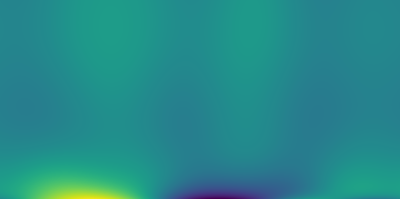
\includegraphics[interpolate=false,width=1.000000in,height=1.000000in]{burgers_exact_pred_0.1-img0.png}}%
\end{pgfscope}%
\begin{pgfscope}%
\pgfsetbuttcap%
\pgfsetroundjoin%
\definecolor{currentfill}{rgb}{0.000000,0.000000,0.000000}%
\pgfsetfillcolor{currentfill}%
\pgfsetlinewidth{0.803000pt}%
\definecolor{currentstroke}{rgb}{0.000000,0.000000,0.000000}%
\pgfsetstrokecolor{currentstroke}%
\pgfsetdash{}{0pt}%
\pgfsys@defobject{currentmarker}{\pgfqpoint{0.000000in}{-0.048611in}}{\pgfqpoint{0.000000in}{0.000000in}}{%
\pgfpathmoveto{\pgfqpoint{0.000000in}{0.000000in}}%
\pgfpathlineto{\pgfqpoint{0.000000in}{-0.048611in}}%
\pgfusepath{stroke,fill}%
}%
\begin{pgfscope}%
\pgfsys@transformshift{0.726837in}{0.517039in}%
\pgfsys@useobject{currentmarker}{}%
\end{pgfscope}%
\end{pgfscope}%
\begin{pgfscope}%
\definecolor{textcolor}{rgb}{0.000000,0.000000,0.000000}%
\pgfsetstrokecolor{textcolor}%
\pgfsetfillcolor{textcolor}%
\pgftext[x=0.726837in,y=0.419816in,,top]{\color{textcolor}\rmfamily\fontsize{12.000000}{14.400000}\selectfont 0}%
\end{pgfscope}%
\begin{pgfscope}%
\pgfsetbuttcap%
\pgfsetroundjoin%
\definecolor{currentfill}{rgb}{0.000000,0.000000,0.000000}%
\pgfsetfillcolor{currentfill}%
\pgfsetlinewidth{0.803000pt}%
\definecolor{currentstroke}{rgb}{0.000000,0.000000,0.000000}%
\pgfsetstrokecolor{currentstroke}%
\pgfsetdash{}{0pt}%
\pgfsys@defobject{currentmarker}{\pgfqpoint{0.000000in}{-0.048611in}}{\pgfqpoint{0.000000in}{0.000000in}}{%
\pgfpathmoveto{\pgfqpoint{0.000000in}{0.000000in}}%
\pgfpathlineto{\pgfqpoint{0.000000in}{-0.048611in}}%
\pgfusepath{stroke,fill}%
}%
\begin{pgfscope}%
\pgfsys@transformshift{1.495229in}{0.517039in}%
\pgfsys@useobject{currentmarker}{}%
\end{pgfscope}%
\end{pgfscope}%
\begin{pgfscope}%
\definecolor{textcolor}{rgb}{0.000000,0.000000,0.000000}%
\pgfsetstrokecolor{textcolor}%
\pgfsetfillcolor{textcolor}%
\pgftext[x=1.495229in,y=0.419816in,,top]{\color{textcolor}\rmfamily\fontsize{12.000000}{14.400000}\selectfont 1}%
\end{pgfscope}%
\begin{pgfscope}%
\pgfsetbuttcap%
\pgfsetroundjoin%
\definecolor{currentfill}{rgb}{0.000000,0.000000,0.000000}%
\pgfsetfillcolor{currentfill}%
\pgfsetlinewidth{0.803000pt}%
\definecolor{currentstroke}{rgb}{0.000000,0.000000,0.000000}%
\pgfsetstrokecolor{currentstroke}%
\pgfsetdash{}{0pt}%
\pgfsys@defobject{currentmarker}{\pgfqpoint{0.000000in}{-0.048611in}}{\pgfqpoint{0.000000in}{0.000000in}}{%
\pgfpathmoveto{\pgfqpoint{0.000000in}{0.000000in}}%
\pgfpathlineto{\pgfqpoint{0.000000in}{-0.048611in}}%
\pgfusepath{stroke,fill}%
}%
\begin{pgfscope}%
\pgfsys@transformshift{2.263621in}{0.517039in}%
\pgfsys@useobject{currentmarker}{}%
\end{pgfscope}%
\end{pgfscope}%
\begin{pgfscope}%
\definecolor{textcolor}{rgb}{0.000000,0.000000,0.000000}%
\pgfsetstrokecolor{textcolor}%
\pgfsetfillcolor{textcolor}%
\pgftext[x=2.263621in,y=0.419816in,,top]{\color{textcolor}\rmfamily\fontsize{12.000000}{14.400000}\selectfont 2}%
\end{pgfscope}%
\begin{pgfscope}%
\definecolor{textcolor}{rgb}{0.000000,0.000000,0.000000}%
\pgfsetstrokecolor{textcolor}%
\pgfsetfillcolor{textcolor}%
\pgftext[x=1.495229in,y=0.202965in,,top]{\color{textcolor}\rmfamily\fontsize{12.000000}{14.400000}\selectfont Space}%
\end{pgfscope}%
\begin{pgfscope}%
\pgfsetbuttcap%
\pgfsetroundjoin%
\definecolor{currentfill}{rgb}{0.000000,0.000000,0.000000}%
\pgfsetfillcolor{currentfill}%
\pgfsetlinewidth{0.803000pt}%
\definecolor{currentstroke}{rgb}{0.000000,0.000000,0.000000}%
\pgfsetstrokecolor{currentstroke}%
\pgfsetdash{}{0pt}%
\pgfsys@defobject{currentmarker}{\pgfqpoint{-0.048611in}{0.000000in}}{\pgfqpoint{-0.000000in}{0.000000in}}{%
\pgfpathmoveto{\pgfqpoint{-0.000000in}{0.000000in}}%
\pgfpathlineto{\pgfqpoint{-0.048611in}{0.000000in}}%
\pgfusepath{stroke,fill}%
}%
\begin{pgfscope}%
\pgfsys@transformshift{0.726837in}{0.517039in}%
\pgfsys@useobject{currentmarker}{}%
\end{pgfscope}%
\end{pgfscope}%
\begin{pgfscope}%
\definecolor{textcolor}{rgb}{0.000000,0.000000,0.000000}%
\pgfsetstrokecolor{textcolor}%
\pgfsetfillcolor{textcolor}%
\pgftext[x=0.364559in, y=0.453725in, left, base]{\color{textcolor}\rmfamily\fontsize{12.000000}{14.400000}\selectfont 0.0}%
\end{pgfscope}%
\begin{pgfscope}%
\pgfsetbuttcap%
\pgfsetroundjoin%
\definecolor{currentfill}{rgb}{0.000000,0.000000,0.000000}%
\pgfsetfillcolor{currentfill}%
\pgfsetlinewidth{0.803000pt}%
\definecolor{currentstroke}{rgb}{0.000000,0.000000,0.000000}%
\pgfsetstrokecolor{currentstroke}%
\pgfsetdash{}{0pt}%
\pgfsys@defobject{currentmarker}{\pgfqpoint{-0.048611in}{0.000000in}}{\pgfqpoint{-0.000000in}{0.000000in}}{%
\pgfpathmoveto{\pgfqpoint{-0.000000in}{0.000000in}}%
\pgfpathlineto{\pgfqpoint{-0.048611in}{0.000000in}}%
\pgfusepath{stroke,fill}%
}%
\begin{pgfscope}%
\pgfsys@transformshift{0.726837in}{0.861533in}%
\pgfsys@useobject{currentmarker}{}%
\end{pgfscope}%
\end{pgfscope}%
\begin{pgfscope}%
\definecolor{textcolor}{rgb}{0.000000,0.000000,0.000000}%
\pgfsetstrokecolor{textcolor}%
\pgfsetfillcolor{textcolor}%
\pgftext[x=0.364559in, y=0.798219in, left, base]{\color{textcolor}\rmfamily\fontsize{12.000000}{14.400000}\selectfont 2.5}%
\end{pgfscope}%
\begin{pgfscope}%
\pgfsetbuttcap%
\pgfsetroundjoin%
\definecolor{currentfill}{rgb}{0.000000,0.000000,0.000000}%
\pgfsetfillcolor{currentfill}%
\pgfsetlinewidth{0.803000pt}%
\definecolor{currentstroke}{rgb}{0.000000,0.000000,0.000000}%
\pgfsetstrokecolor{currentstroke}%
\pgfsetdash{}{0pt}%
\pgfsys@defobject{currentmarker}{\pgfqpoint{-0.048611in}{0.000000in}}{\pgfqpoint{-0.000000in}{0.000000in}}{%
\pgfpathmoveto{\pgfqpoint{-0.000000in}{0.000000in}}%
\pgfpathlineto{\pgfqpoint{-0.048611in}{0.000000in}}%
\pgfusepath{stroke,fill}%
}%
\begin{pgfscope}%
\pgfsys@transformshift{0.726837in}{1.206027in}%
\pgfsys@useobject{currentmarker}{}%
\end{pgfscope}%
\end{pgfscope}%
\begin{pgfscope}%
\definecolor{textcolor}{rgb}{0.000000,0.000000,0.000000}%
\pgfsetstrokecolor{textcolor}%
\pgfsetfillcolor{textcolor}%
\pgftext[x=0.364559in, y=1.142714in, left, base]{\color{textcolor}\rmfamily\fontsize{12.000000}{14.400000}\selectfont 5.0}%
\end{pgfscope}%
\begin{pgfscope}%
\pgfsetbuttcap%
\pgfsetroundjoin%
\definecolor{currentfill}{rgb}{0.000000,0.000000,0.000000}%
\pgfsetfillcolor{currentfill}%
\pgfsetlinewidth{0.803000pt}%
\definecolor{currentstroke}{rgb}{0.000000,0.000000,0.000000}%
\pgfsetstrokecolor{currentstroke}%
\pgfsetdash{}{0pt}%
\pgfsys@defobject{currentmarker}{\pgfqpoint{-0.048611in}{0.000000in}}{\pgfqpoint{-0.000000in}{0.000000in}}{%
\pgfpathmoveto{\pgfqpoint{-0.000000in}{0.000000in}}%
\pgfpathlineto{\pgfqpoint{-0.048611in}{0.000000in}}%
\pgfusepath{stroke,fill}%
}%
\begin{pgfscope}%
\pgfsys@transformshift{0.726837in}{1.550522in}%
\pgfsys@useobject{currentmarker}{}%
\end{pgfscope}%
\end{pgfscope}%
\begin{pgfscope}%
\definecolor{textcolor}{rgb}{0.000000,0.000000,0.000000}%
\pgfsetstrokecolor{textcolor}%
\pgfsetfillcolor{textcolor}%
\pgftext[x=0.364559in, y=1.487208in, left, base]{\color{textcolor}\rmfamily\fontsize{12.000000}{14.400000}\selectfont 7.5}%
\end{pgfscope}%
\begin{pgfscope}%
\pgfsetbuttcap%
\pgfsetroundjoin%
\definecolor{currentfill}{rgb}{0.000000,0.000000,0.000000}%
\pgfsetfillcolor{currentfill}%
\pgfsetlinewidth{0.803000pt}%
\definecolor{currentstroke}{rgb}{0.000000,0.000000,0.000000}%
\pgfsetstrokecolor{currentstroke}%
\pgfsetdash{}{0pt}%
\pgfsys@defobject{currentmarker}{\pgfqpoint{-0.048611in}{0.000000in}}{\pgfqpoint{-0.000000in}{0.000000in}}{%
\pgfpathmoveto{\pgfqpoint{-0.000000in}{0.000000in}}%
\pgfpathlineto{\pgfqpoint{-0.048611in}{0.000000in}}%
\pgfusepath{stroke,fill}%
}%
\begin{pgfscope}%
\pgfsys@transformshift{0.726837in}{1.895016in}%
\pgfsys@useobject{currentmarker}{}%
\end{pgfscope}%
\end{pgfscope}%
\begin{pgfscope}%
\definecolor{textcolor}{rgb}{0.000000,0.000000,0.000000}%
\pgfsetstrokecolor{textcolor}%
\pgfsetfillcolor{textcolor}%
\pgftext[x=0.258521in, y=1.831702in, left, base]{\color{textcolor}\rmfamily\fontsize{12.000000}{14.400000}\selectfont 10.0}%
\end{pgfscope}%
\begin{pgfscope}%
\definecolor{textcolor}{rgb}{0.000000,0.000000,0.000000}%
\pgfsetstrokecolor{textcolor}%
\pgfsetfillcolor{textcolor}%
\pgftext[x=0.202965in,y=1.206027in,,bottom,rotate=90.000000]{\color{textcolor}\rmfamily\fontsize{12.000000}{14.400000}\selectfont Time}%
\end{pgfscope}%
\begin{pgfscope}%
\pgfsetrectcap%
\pgfsetmiterjoin%
\pgfsetlinewidth{0.803000pt}%
\definecolor{currentstroke}{rgb}{0.000000,0.000000,0.000000}%
\pgfsetstrokecolor{currentstroke}%
\pgfsetdash{}{0pt}%
\pgfpathmoveto{\pgfqpoint{0.726837in}{0.517039in}}%
\pgfpathlineto{\pgfqpoint{0.726837in}{1.895016in}}%
\pgfusepath{stroke}%
\end{pgfscope}%
\begin{pgfscope}%
\pgfsetrectcap%
\pgfsetmiterjoin%
\pgfsetlinewidth{0.803000pt}%
\definecolor{currentstroke}{rgb}{0.000000,0.000000,0.000000}%
\pgfsetstrokecolor{currentstroke}%
\pgfsetdash{}{0pt}%
\pgfpathmoveto{\pgfqpoint{2.263621in}{0.517039in}}%
\pgfpathlineto{\pgfqpoint{2.263621in}{1.895016in}}%
\pgfusepath{stroke}%
\end{pgfscope}%
\begin{pgfscope}%
\pgfsetrectcap%
\pgfsetmiterjoin%
\pgfsetlinewidth{0.803000pt}%
\definecolor{currentstroke}{rgb}{0.000000,0.000000,0.000000}%
\pgfsetstrokecolor{currentstroke}%
\pgfsetdash{}{0pt}%
\pgfpathmoveto{\pgfqpoint{0.726837in}{0.517039in}}%
\pgfpathlineto{\pgfqpoint{2.263621in}{0.517039in}}%
\pgfusepath{stroke}%
\end{pgfscope}%
\begin{pgfscope}%
\pgfsetrectcap%
\pgfsetmiterjoin%
\pgfsetlinewidth{0.803000pt}%
\definecolor{currentstroke}{rgb}{0.000000,0.000000,0.000000}%
\pgfsetstrokecolor{currentstroke}%
\pgfsetdash{}{0pt}%
\pgfpathmoveto{\pgfqpoint{0.726837in}{1.895016in}}%
\pgfpathlineto{\pgfqpoint{2.263621in}{1.895016in}}%
\pgfusepath{stroke}%
\end{pgfscope}%
\begin{pgfscope}%
\pgfsetbuttcap%
\pgfsetmiterjoin%
\pgfsetlinewidth{0.000000pt}%
\definecolor{currentstroke}{rgb}{0.000000,0.000000,0.000000}%
\pgfsetstrokecolor{currentstroke}%
\pgfsetstrokeopacity{0.000000}%
\pgfsetdash{}{0pt}%
\pgfpathmoveto{\pgfqpoint{2.393479in}{0.517039in}}%
\pgfpathlineto{\pgfqpoint{2.462378in}{0.517039in}}%
\pgfpathlineto{\pgfqpoint{2.462378in}{1.895016in}}%
\pgfpathlineto{\pgfqpoint{2.393479in}{1.895016in}}%
\pgfpathlineto{\pgfqpoint{2.393479in}{0.517039in}}%
\pgfpathclose%
\pgfusepath{}%
\end{pgfscope}%
\begin{pgfscope}%
\pgfsys@transformshift{2.390000in}{0.520000in}%
\pgftext[left,bottom]{\includegraphics[interpolate=true,width=0.070000in,height=1.380000in]{burgers_exact_pred_0.1-img1.png}}%
\end{pgfscope}%
\begin{pgfscope}%
\pgfsetbuttcap%
\pgfsetroundjoin%
\definecolor{currentfill}{rgb}{0.000000,0.000000,0.000000}%
\pgfsetfillcolor{currentfill}%
\pgfsetlinewidth{0.803000pt}%
\definecolor{currentstroke}{rgb}{0.000000,0.000000,0.000000}%
\pgfsetstrokecolor{currentstroke}%
\pgfsetdash{}{0pt}%
\pgfsys@defobject{currentmarker}{\pgfqpoint{0.000000in}{0.000000in}}{\pgfqpoint{0.048611in}{0.000000in}}{%
\pgfpathmoveto{\pgfqpoint{0.000000in}{0.000000in}}%
\pgfpathlineto{\pgfqpoint{0.048611in}{0.000000in}}%
\pgfusepath{stroke,fill}%
}%
\begin{pgfscope}%
\pgfsys@transformshift{2.462378in}{0.613156in}%
\pgfsys@useobject{currentmarker}{}%
\end{pgfscope}%
\end{pgfscope}%
\begin{pgfscope}%
\definecolor{textcolor}{rgb}{0.000000,0.000000,0.000000}%
\pgfsetstrokecolor{textcolor}%
\pgfsetfillcolor{textcolor}%
\pgftext[x=2.559601in, y=0.549842in, left, base]{\color{textcolor}\rmfamily\fontsize{12.000000}{14.400000}\selectfont \ensuremath{-}0.2}%
\end{pgfscope}%
\begin{pgfscope}%
\pgfsetbuttcap%
\pgfsetroundjoin%
\definecolor{currentfill}{rgb}{0.000000,0.000000,0.000000}%
\pgfsetfillcolor{currentfill}%
\pgfsetlinewidth{0.803000pt}%
\definecolor{currentstroke}{rgb}{0.000000,0.000000,0.000000}%
\pgfsetstrokecolor{currentstroke}%
\pgfsetdash{}{0pt}%
\pgfsys@defobject{currentmarker}{\pgfqpoint{0.000000in}{0.000000in}}{\pgfqpoint{0.048611in}{0.000000in}}{%
\pgfpathmoveto{\pgfqpoint{0.000000in}{0.000000in}}%
\pgfpathlineto{\pgfqpoint{0.048611in}{0.000000in}}%
\pgfusepath{stroke,fill}%
}%
\begin{pgfscope}%
\pgfsys@transformshift{2.462378in}{1.206027in}%
\pgfsys@useobject{currentmarker}{}%
\end{pgfscope}%
\end{pgfscope}%
\begin{pgfscope}%
\definecolor{textcolor}{rgb}{0.000000,0.000000,0.000000}%
\pgfsetstrokecolor{textcolor}%
\pgfsetfillcolor{textcolor}%
\pgftext[x=2.559601in, y=1.142714in, left, base]{\color{textcolor}\rmfamily\fontsize{12.000000}{14.400000}\selectfont 0.0}%
\end{pgfscope}%
\begin{pgfscope}%
\pgfsetbuttcap%
\pgfsetroundjoin%
\definecolor{currentfill}{rgb}{0.000000,0.000000,0.000000}%
\pgfsetfillcolor{currentfill}%
\pgfsetlinewidth{0.803000pt}%
\definecolor{currentstroke}{rgb}{0.000000,0.000000,0.000000}%
\pgfsetstrokecolor{currentstroke}%
\pgfsetdash{}{0pt}%
\pgfsys@defobject{currentmarker}{\pgfqpoint{0.000000in}{0.000000in}}{\pgfqpoint{0.048611in}{0.000000in}}{%
\pgfpathmoveto{\pgfqpoint{0.000000in}{0.000000in}}%
\pgfpathlineto{\pgfqpoint{0.048611in}{0.000000in}}%
\pgfusepath{stroke,fill}%
}%
\begin{pgfscope}%
\pgfsys@transformshift{2.462378in}{1.798899in}%
\pgfsys@useobject{currentmarker}{}%
\end{pgfscope}%
\end{pgfscope}%
\begin{pgfscope}%
\definecolor{textcolor}{rgb}{0.000000,0.000000,0.000000}%
\pgfsetstrokecolor{textcolor}%
\pgfsetfillcolor{textcolor}%
\pgftext[x=2.559601in, y=1.735585in, left, base]{\color{textcolor}\rmfamily\fontsize{12.000000}{14.400000}\selectfont 0.2}%
\end{pgfscope}%
\begin{pgfscope}%
\pgfsetrectcap%
\pgfsetmiterjoin%
\pgfsetlinewidth{0.803000pt}%
\definecolor{currentstroke}{rgb}{0.000000,0.000000,0.000000}%
\pgfsetstrokecolor{currentstroke}%
\pgfsetdash{}{0pt}%
\pgfpathmoveto{\pgfqpoint{2.393479in}{0.517039in}}%
\pgfpathlineto{\pgfqpoint{2.427929in}{0.517039in}}%
\pgfpathlineto{\pgfqpoint{2.462378in}{0.517039in}}%
\pgfpathlineto{\pgfqpoint{2.462378in}{1.895016in}}%
\pgfpathlineto{\pgfqpoint{2.427929in}{1.895016in}}%
\pgfpathlineto{\pgfqpoint{2.393479in}{1.895016in}}%
\pgfpathlineto{\pgfqpoint{2.393479in}{0.517039in}}%
\pgfpathclose%
\pgfusepath{stroke}%
\end{pgfscope}%
\end{pgfpicture}%
\makeatother%
\endgroup%

      \end{adjustbox}
      \caption{The prediction for \(\nu=0.1\)}\label{fig:sc2_exact_pred_0.1}
    \end{subfigure}
    \begin{subfigure}{0.32\linewidth}
      \begin{adjustbox}{width=\linewidth}
        \begingroup%
\makeatletter%
\begin{pgfpicture}%
\pgfpathrectangle{\pgfpointorigin}{\pgfqpoint{3.000000in}{2.000000in}}%
\pgfusepath{use as bounding box, clip}%
\begin{pgfscope}%
\pgfsetbuttcap%
\pgfsetmiterjoin%
\pgfsetlinewidth{0.000000pt}%
\definecolor{currentstroke}{rgb}{0.000000,0.000000,0.000000}%
\pgfsetstrokecolor{currentstroke}%
\pgfsetstrokeopacity{0.000000}%
\pgfsetdash{}{0pt}%
\pgfpathmoveto{\pgfqpoint{0.000000in}{0.000000in}}%
\pgfpathlineto{\pgfqpoint{3.000000in}{0.000000in}}%
\pgfpathlineto{\pgfqpoint{3.000000in}{2.000000in}}%
\pgfpathlineto{\pgfqpoint{0.000000in}{2.000000in}}%
\pgfpathlineto{\pgfqpoint{0.000000in}{0.000000in}}%
\pgfpathclose%
\pgfusepath{}%
\end{pgfscope}%
\begin{pgfscope}%
\pgfsetbuttcap%
\pgfsetmiterjoin%
\pgfsetlinewidth{0.000000pt}%
\definecolor{currentstroke}{rgb}{0.000000,0.000000,0.000000}%
\pgfsetstrokecolor{currentstroke}%
\pgfsetstrokeopacity{0.000000}%
\pgfsetdash{}{0pt}%
\pgfpathmoveto{\pgfqpoint{0.726837in}{0.517039in}}%
\pgfpathlineto{\pgfqpoint{2.263621in}{0.517039in}}%
\pgfpathlineto{\pgfqpoint{2.263621in}{1.895016in}}%
\pgfpathlineto{\pgfqpoint{0.726837in}{1.895016in}}%
\pgfpathlineto{\pgfqpoint{0.726837in}{0.517039in}}%
\pgfpathclose%
\pgfusepath{}%
\end{pgfscope}%
\begin{pgfscope}%
\pgfpathrectangle{\pgfqpoint{0.726837in}{0.517039in}}{\pgfqpoint{1.536784in}{1.377978in}}%
\pgfusepath{clip}%
\pgfsys@transformcm{1.536784}{0.000000}{0.000000}{1.377978}{0.726837in}{0.517039in}%
\pgftext[left,bottom]{\includegraphics[interpolate=false,width=1.000000in,height=1.000000in]{burgers_exact_diff_0.1-img0.png}}%
\end{pgfscope}%
\begin{pgfscope}%
\pgfsetbuttcap%
\pgfsetroundjoin%
\definecolor{currentfill}{rgb}{0.000000,0.000000,0.000000}%
\pgfsetfillcolor{currentfill}%
\pgfsetlinewidth{0.803000pt}%
\definecolor{currentstroke}{rgb}{0.000000,0.000000,0.000000}%
\pgfsetstrokecolor{currentstroke}%
\pgfsetdash{}{0pt}%
\pgfsys@defobject{currentmarker}{\pgfqpoint{0.000000in}{-0.048611in}}{\pgfqpoint{0.000000in}{0.000000in}}{%
\pgfpathmoveto{\pgfqpoint{0.000000in}{0.000000in}}%
\pgfpathlineto{\pgfqpoint{0.000000in}{-0.048611in}}%
\pgfusepath{stroke,fill}%
}%
\begin{pgfscope}%
\pgfsys@transformshift{0.726837in}{0.517039in}%
\pgfsys@useobject{currentmarker}{}%
\end{pgfscope}%
\end{pgfscope}%
\begin{pgfscope}%
\definecolor{textcolor}{rgb}{0.000000,0.000000,0.000000}%
\pgfsetstrokecolor{textcolor}%
\pgfsetfillcolor{textcolor}%
\pgftext[x=0.726837in,y=0.419816in,,top]{\color{textcolor}{\rmfamily\fontsize{12.000000}{14.400000}\selectfont\catcode`\^=\active\def^{\ifmmode\sp\else\^{}\fi}\catcode`\%=\active\def%{\%}0}}%
\end{pgfscope}%
\begin{pgfscope}%
\pgfsetbuttcap%
\pgfsetroundjoin%
\definecolor{currentfill}{rgb}{0.000000,0.000000,0.000000}%
\pgfsetfillcolor{currentfill}%
\pgfsetlinewidth{0.803000pt}%
\definecolor{currentstroke}{rgb}{0.000000,0.000000,0.000000}%
\pgfsetstrokecolor{currentstroke}%
\pgfsetdash{}{0pt}%
\pgfsys@defobject{currentmarker}{\pgfqpoint{0.000000in}{-0.048611in}}{\pgfqpoint{0.000000in}{0.000000in}}{%
\pgfpathmoveto{\pgfqpoint{0.000000in}{0.000000in}}%
\pgfpathlineto{\pgfqpoint{0.000000in}{-0.048611in}}%
\pgfusepath{stroke,fill}%
}%
\begin{pgfscope}%
\pgfsys@transformshift{1.495229in}{0.517039in}%
\pgfsys@useobject{currentmarker}{}%
\end{pgfscope}%
\end{pgfscope}%
\begin{pgfscope}%
\definecolor{textcolor}{rgb}{0.000000,0.000000,0.000000}%
\pgfsetstrokecolor{textcolor}%
\pgfsetfillcolor{textcolor}%
\pgftext[x=1.495229in,y=0.419816in,,top]{\color{textcolor}{\rmfamily\fontsize{12.000000}{14.400000}\selectfont\catcode`\^=\active\def^{\ifmmode\sp\else\^{}\fi}\catcode`\%=\active\def%{\%}1}}%
\end{pgfscope}%
\begin{pgfscope}%
\pgfsetbuttcap%
\pgfsetroundjoin%
\definecolor{currentfill}{rgb}{0.000000,0.000000,0.000000}%
\pgfsetfillcolor{currentfill}%
\pgfsetlinewidth{0.803000pt}%
\definecolor{currentstroke}{rgb}{0.000000,0.000000,0.000000}%
\pgfsetstrokecolor{currentstroke}%
\pgfsetdash{}{0pt}%
\pgfsys@defobject{currentmarker}{\pgfqpoint{0.000000in}{-0.048611in}}{\pgfqpoint{0.000000in}{0.000000in}}{%
\pgfpathmoveto{\pgfqpoint{0.000000in}{0.000000in}}%
\pgfpathlineto{\pgfqpoint{0.000000in}{-0.048611in}}%
\pgfusepath{stroke,fill}%
}%
\begin{pgfscope}%
\pgfsys@transformshift{2.263621in}{0.517039in}%
\pgfsys@useobject{currentmarker}{}%
\end{pgfscope}%
\end{pgfscope}%
\begin{pgfscope}%
\definecolor{textcolor}{rgb}{0.000000,0.000000,0.000000}%
\pgfsetstrokecolor{textcolor}%
\pgfsetfillcolor{textcolor}%
\pgftext[x=2.263621in,y=0.419816in,,top]{\color{textcolor}{\rmfamily\fontsize{12.000000}{14.400000}\selectfont\catcode`\^=\active\def^{\ifmmode\sp\else\^{}\fi}\catcode`\%=\active\def%{\%}2}}%
\end{pgfscope}%
\begin{pgfscope}%
\definecolor{textcolor}{rgb}{0.000000,0.000000,0.000000}%
\pgfsetstrokecolor{textcolor}%
\pgfsetfillcolor{textcolor}%
\pgftext[x=1.495229in,y=0.202965in,,top]{\color{textcolor}{\rmfamily\fontsize{12.000000}{14.400000}\selectfont\catcode`\^=\active\def^{\ifmmode\sp\else\^{}\fi}\catcode`\%=\active\def%{\%}Space}}%
\end{pgfscope}%
\begin{pgfscope}%
\pgfsetbuttcap%
\pgfsetroundjoin%
\definecolor{currentfill}{rgb}{0.000000,0.000000,0.000000}%
\pgfsetfillcolor{currentfill}%
\pgfsetlinewidth{0.803000pt}%
\definecolor{currentstroke}{rgb}{0.000000,0.000000,0.000000}%
\pgfsetstrokecolor{currentstroke}%
\pgfsetdash{}{0pt}%
\pgfsys@defobject{currentmarker}{\pgfqpoint{-0.048611in}{0.000000in}}{\pgfqpoint{-0.000000in}{0.000000in}}{%
\pgfpathmoveto{\pgfqpoint{-0.000000in}{0.000000in}}%
\pgfpathlineto{\pgfqpoint{-0.048611in}{0.000000in}}%
\pgfusepath{stroke,fill}%
}%
\begin{pgfscope}%
\pgfsys@transformshift{0.726837in}{0.517039in}%
\pgfsys@useobject{currentmarker}{}%
\end{pgfscope}%
\end{pgfscope}%
\begin{pgfscope}%
\definecolor{textcolor}{rgb}{0.000000,0.000000,0.000000}%
\pgfsetstrokecolor{textcolor}%
\pgfsetfillcolor{textcolor}%
\pgftext[x=0.364559in, y=0.453725in, left, base]{\color{textcolor}{\rmfamily\fontsize{12.000000}{14.400000}\selectfont\catcode`\^=\active\def^{\ifmmode\sp\else\^{}\fi}\catcode`\%=\active\def%{\%}0.0}}%
\end{pgfscope}%
\begin{pgfscope}%
\pgfsetbuttcap%
\pgfsetroundjoin%
\definecolor{currentfill}{rgb}{0.000000,0.000000,0.000000}%
\pgfsetfillcolor{currentfill}%
\pgfsetlinewidth{0.803000pt}%
\definecolor{currentstroke}{rgb}{0.000000,0.000000,0.000000}%
\pgfsetstrokecolor{currentstroke}%
\pgfsetdash{}{0pt}%
\pgfsys@defobject{currentmarker}{\pgfqpoint{-0.048611in}{0.000000in}}{\pgfqpoint{-0.000000in}{0.000000in}}{%
\pgfpathmoveto{\pgfqpoint{-0.000000in}{0.000000in}}%
\pgfpathlineto{\pgfqpoint{-0.048611in}{0.000000in}}%
\pgfusepath{stroke,fill}%
}%
\begin{pgfscope}%
\pgfsys@transformshift{0.726837in}{0.861533in}%
\pgfsys@useobject{currentmarker}{}%
\end{pgfscope}%
\end{pgfscope}%
\begin{pgfscope}%
\definecolor{textcolor}{rgb}{0.000000,0.000000,0.000000}%
\pgfsetstrokecolor{textcolor}%
\pgfsetfillcolor{textcolor}%
\pgftext[x=0.364559in, y=0.798219in, left, base]{\color{textcolor}{\rmfamily\fontsize{12.000000}{14.400000}\selectfont\catcode`\^=\active\def^{\ifmmode\sp\else\^{}\fi}\catcode`\%=\active\def%{\%}2.5}}%
\end{pgfscope}%
\begin{pgfscope}%
\pgfsetbuttcap%
\pgfsetroundjoin%
\definecolor{currentfill}{rgb}{0.000000,0.000000,0.000000}%
\pgfsetfillcolor{currentfill}%
\pgfsetlinewidth{0.803000pt}%
\definecolor{currentstroke}{rgb}{0.000000,0.000000,0.000000}%
\pgfsetstrokecolor{currentstroke}%
\pgfsetdash{}{0pt}%
\pgfsys@defobject{currentmarker}{\pgfqpoint{-0.048611in}{0.000000in}}{\pgfqpoint{-0.000000in}{0.000000in}}{%
\pgfpathmoveto{\pgfqpoint{-0.000000in}{0.000000in}}%
\pgfpathlineto{\pgfqpoint{-0.048611in}{0.000000in}}%
\pgfusepath{stroke,fill}%
}%
\begin{pgfscope}%
\pgfsys@transformshift{0.726837in}{1.206027in}%
\pgfsys@useobject{currentmarker}{}%
\end{pgfscope}%
\end{pgfscope}%
\begin{pgfscope}%
\definecolor{textcolor}{rgb}{0.000000,0.000000,0.000000}%
\pgfsetstrokecolor{textcolor}%
\pgfsetfillcolor{textcolor}%
\pgftext[x=0.364559in, y=1.142714in, left, base]{\color{textcolor}{\rmfamily\fontsize{12.000000}{14.400000}\selectfont\catcode`\^=\active\def^{\ifmmode\sp\else\^{}\fi}\catcode`\%=\active\def%{\%}5.0}}%
\end{pgfscope}%
\begin{pgfscope}%
\pgfsetbuttcap%
\pgfsetroundjoin%
\definecolor{currentfill}{rgb}{0.000000,0.000000,0.000000}%
\pgfsetfillcolor{currentfill}%
\pgfsetlinewidth{0.803000pt}%
\definecolor{currentstroke}{rgb}{0.000000,0.000000,0.000000}%
\pgfsetstrokecolor{currentstroke}%
\pgfsetdash{}{0pt}%
\pgfsys@defobject{currentmarker}{\pgfqpoint{-0.048611in}{0.000000in}}{\pgfqpoint{-0.000000in}{0.000000in}}{%
\pgfpathmoveto{\pgfqpoint{-0.000000in}{0.000000in}}%
\pgfpathlineto{\pgfqpoint{-0.048611in}{0.000000in}}%
\pgfusepath{stroke,fill}%
}%
\begin{pgfscope}%
\pgfsys@transformshift{0.726837in}{1.550522in}%
\pgfsys@useobject{currentmarker}{}%
\end{pgfscope}%
\end{pgfscope}%
\begin{pgfscope}%
\definecolor{textcolor}{rgb}{0.000000,0.000000,0.000000}%
\pgfsetstrokecolor{textcolor}%
\pgfsetfillcolor{textcolor}%
\pgftext[x=0.364559in, y=1.487208in, left, base]{\color{textcolor}{\rmfamily\fontsize{12.000000}{14.400000}\selectfont\catcode`\^=\active\def^{\ifmmode\sp\else\^{}\fi}\catcode`\%=\active\def%{\%}7.5}}%
\end{pgfscope}%
\begin{pgfscope}%
\pgfsetbuttcap%
\pgfsetroundjoin%
\definecolor{currentfill}{rgb}{0.000000,0.000000,0.000000}%
\pgfsetfillcolor{currentfill}%
\pgfsetlinewidth{0.803000pt}%
\definecolor{currentstroke}{rgb}{0.000000,0.000000,0.000000}%
\pgfsetstrokecolor{currentstroke}%
\pgfsetdash{}{0pt}%
\pgfsys@defobject{currentmarker}{\pgfqpoint{-0.048611in}{0.000000in}}{\pgfqpoint{-0.000000in}{0.000000in}}{%
\pgfpathmoveto{\pgfqpoint{-0.000000in}{0.000000in}}%
\pgfpathlineto{\pgfqpoint{-0.048611in}{0.000000in}}%
\pgfusepath{stroke,fill}%
}%
\begin{pgfscope}%
\pgfsys@transformshift{0.726837in}{1.895016in}%
\pgfsys@useobject{currentmarker}{}%
\end{pgfscope}%
\end{pgfscope}%
\begin{pgfscope}%
\definecolor{textcolor}{rgb}{0.000000,0.000000,0.000000}%
\pgfsetstrokecolor{textcolor}%
\pgfsetfillcolor{textcolor}%
\pgftext[x=0.258521in, y=1.831702in, left, base]{\color{textcolor}{\rmfamily\fontsize{12.000000}{14.400000}\selectfont\catcode`\^=\active\def^{\ifmmode\sp\else\^{}\fi}\catcode`\%=\active\def%{\%}10.0}}%
\end{pgfscope}%
\begin{pgfscope}%
\definecolor{textcolor}{rgb}{0.000000,0.000000,0.000000}%
\pgfsetstrokecolor{textcolor}%
\pgfsetfillcolor{textcolor}%
\pgftext[x=0.202965in,y=1.206027in,,bottom,rotate=90.000000]{\color{textcolor}{\rmfamily\fontsize{12.000000}{14.400000}\selectfont\catcode`\^=\active\def^{\ifmmode\sp\else\^{}\fi}\catcode`\%=\active\def%{\%}Time}}%
\end{pgfscope}%
\begin{pgfscope}%
\pgfsetrectcap%
\pgfsetmiterjoin%
\pgfsetlinewidth{0.803000pt}%
\definecolor{currentstroke}{rgb}{0.000000,0.000000,0.000000}%
\pgfsetstrokecolor{currentstroke}%
\pgfsetdash{}{0pt}%
\pgfpathmoveto{\pgfqpoint{0.726837in}{0.517039in}}%
\pgfpathlineto{\pgfqpoint{0.726837in}{1.895016in}}%
\pgfusepath{stroke}%
\end{pgfscope}%
\begin{pgfscope}%
\pgfsetrectcap%
\pgfsetmiterjoin%
\pgfsetlinewidth{0.803000pt}%
\definecolor{currentstroke}{rgb}{0.000000,0.000000,0.000000}%
\pgfsetstrokecolor{currentstroke}%
\pgfsetdash{}{0pt}%
\pgfpathmoveto{\pgfqpoint{2.263621in}{0.517039in}}%
\pgfpathlineto{\pgfqpoint{2.263621in}{1.895016in}}%
\pgfusepath{stroke}%
\end{pgfscope}%
\begin{pgfscope}%
\pgfsetrectcap%
\pgfsetmiterjoin%
\pgfsetlinewidth{0.803000pt}%
\definecolor{currentstroke}{rgb}{0.000000,0.000000,0.000000}%
\pgfsetstrokecolor{currentstroke}%
\pgfsetdash{}{0pt}%
\pgfpathmoveto{\pgfqpoint{0.726837in}{0.517039in}}%
\pgfpathlineto{\pgfqpoint{2.263621in}{0.517039in}}%
\pgfusepath{stroke}%
\end{pgfscope}%
\begin{pgfscope}%
\pgfsetrectcap%
\pgfsetmiterjoin%
\pgfsetlinewidth{0.803000pt}%
\definecolor{currentstroke}{rgb}{0.000000,0.000000,0.000000}%
\pgfsetstrokecolor{currentstroke}%
\pgfsetdash{}{0pt}%
\pgfpathmoveto{\pgfqpoint{0.726837in}{1.895016in}}%
\pgfpathlineto{\pgfqpoint{2.263621in}{1.895016in}}%
\pgfusepath{stroke}%
\end{pgfscope}%
\begin{pgfscope}%
\pgfsetbuttcap%
\pgfsetmiterjoin%
\pgfsetlinewidth{0.000000pt}%
\definecolor{currentstroke}{rgb}{0.000000,0.000000,0.000000}%
\pgfsetstrokecolor{currentstroke}%
\pgfsetstrokeopacity{0.000000}%
\pgfsetdash{}{0pt}%
\pgfpathmoveto{\pgfqpoint{2.393479in}{0.517039in}}%
\pgfpathlineto{\pgfqpoint{2.462378in}{0.517039in}}%
\pgfpathlineto{\pgfqpoint{2.462378in}{1.895016in}}%
\pgfpathlineto{\pgfqpoint{2.393479in}{1.895016in}}%
\pgfpathlineto{\pgfqpoint{2.393479in}{0.517039in}}%
\pgfpathclose%
\pgfusepath{}%
\end{pgfscope}%
\begin{pgfscope}%
\pgfsys@transformshift{2.390000in}{0.520000in}%
\pgftext[left,bottom]{\includegraphics[interpolate=true,width=0.070000in,height=1.380000in]{burgers_exact_diff_0.1-img1.png}}%
\end{pgfscope}%
\begin{pgfscope}%
\pgfsetbuttcap%
\pgfsetroundjoin%
\definecolor{currentfill}{rgb}{0.000000,0.000000,0.000000}%
\pgfsetfillcolor{currentfill}%
\pgfsetlinewidth{0.803000pt}%
\definecolor{currentstroke}{rgb}{0.000000,0.000000,0.000000}%
\pgfsetstrokecolor{currentstroke}%
\pgfsetdash{}{0pt}%
\pgfsys@defobject{currentmarker}{\pgfqpoint{0.000000in}{0.000000in}}{\pgfqpoint{0.048611in}{0.000000in}}{%
\pgfpathmoveto{\pgfqpoint{0.000000in}{0.000000in}}%
\pgfpathlineto{\pgfqpoint{0.048611in}{0.000000in}}%
\pgfusepath{stroke,fill}%
}%
\begin{pgfscope}%
\pgfsys@transformshift{2.462378in}{0.572980in}%
\pgfsys@useobject{currentmarker}{}%
\end{pgfscope}%
\end{pgfscope}%
\begin{pgfscope}%
\definecolor{textcolor}{rgb}{0.000000,0.000000,0.000000}%
\pgfsetstrokecolor{textcolor}%
\pgfsetfillcolor{textcolor}%
\pgftext[x=2.559601in, y=0.509667in, left, base]{\color{textcolor}{\rmfamily\fontsize{12.000000}{14.400000}\selectfont\catcode`\^=\active\def^{\ifmmode\sp\else\^{}\fi}\catcode`\%=\active\def%{\%}\ensuremath{-}0.2}}%
\end{pgfscope}%
\begin{pgfscope}%
\pgfsetbuttcap%
\pgfsetroundjoin%
\definecolor{currentfill}{rgb}{0.000000,0.000000,0.000000}%
\pgfsetfillcolor{currentfill}%
\pgfsetlinewidth{0.803000pt}%
\definecolor{currentstroke}{rgb}{0.000000,0.000000,0.000000}%
\pgfsetstrokecolor{currentstroke}%
\pgfsetdash{}{0pt}%
\pgfsys@defobject{currentmarker}{\pgfqpoint{0.000000in}{0.000000in}}{\pgfqpoint{0.048611in}{0.000000in}}{%
\pgfpathmoveto{\pgfqpoint{0.000000in}{0.000000in}}%
\pgfpathlineto{\pgfqpoint{0.048611in}{0.000000in}}%
\pgfusepath{stroke,fill}%
}%
\begin{pgfscope}%
\pgfsys@transformshift{2.462378in}{1.206027in}%
\pgfsys@useobject{currentmarker}{}%
\end{pgfscope}%
\end{pgfscope}%
\begin{pgfscope}%
\definecolor{textcolor}{rgb}{0.000000,0.000000,0.000000}%
\pgfsetstrokecolor{textcolor}%
\pgfsetfillcolor{textcolor}%
\pgftext[x=2.559601in, y=1.142714in, left, base]{\color{textcolor}{\rmfamily\fontsize{12.000000}{14.400000}\selectfont\catcode`\^=\active\def^{\ifmmode\sp\else\^{}\fi}\catcode`\%=\active\def%{\%}0.0}}%
\end{pgfscope}%
\begin{pgfscope}%
\pgfsetbuttcap%
\pgfsetroundjoin%
\definecolor{currentfill}{rgb}{0.000000,0.000000,0.000000}%
\pgfsetfillcolor{currentfill}%
\pgfsetlinewidth{0.803000pt}%
\definecolor{currentstroke}{rgb}{0.000000,0.000000,0.000000}%
\pgfsetstrokecolor{currentstroke}%
\pgfsetdash{}{0pt}%
\pgfsys@defobject{currentmarker}{\pgfqpoint{0.000000in}{0.000000in}}{\pgfqpoint{0.048611in}{0.000000in}}{%
\pgfpathmoveto{\pgfqpoint{0.000000in}{0.000000in}}%
\pgfpathlineto{\pgfqpoint{0.048611in}{0.000000in}}%
\pgfusepath{stroke,fill}%
}%
\begin{pgfscope}%
\pgfsys@transformshift{2.462378in}{1.839074in}%
\pgfsys@useobject{currentmarker}{}%
\end{pgfscope}%
\end{pgfscope}%
\begin{pgfscope}%
\definecolor{textcolor}{rgb}{0.000000,0.000000,0.000000}%
\pgfsetstrokecolor{textcolor}%
\pgfsetfillcolor{textcolor}%
\pgftext[x=2.559601in, y=1.775761in, left, base]{\color{textcolor}{\rmfamily\fontsize{12.000000}{14.400000}\selectfont\catcode`\^=\active\def^{\ifmmode\sp\else\^{}\fi}\catcode`\%=\active\def%{\%}0.2}}%
\end{pgfscope}%
\begin{pgfscope}%
\pgfsetrectcap%
\pgfsetmiterjoin%
\pgfsetlinewidth{0.803000pt}%
\definecolor{currentstroke}{rgb}{0.000000,0.000000,0.000000}%
\pgfsetstrokecolor{currentstroke}%
\pgfsetdash{}{0pt}%
\pgfpathmoveto{\pgfqpoint{2.393479in}{0.517039in}}%
\pgfpathlineto{\pgfqpoint{2.427929in}{0.517039in}}%
\pgfpathlineto{\pgfqpoint{2.462378in}{0.517039in}}%
\pgfpathlineto{\pgfqpoint{2.462378in}{1.895016in}}%
\pgfpathlineto{\pgfqpoint{2.427929in}{1.895016in}}%
\pgfpathlineto{\pgfqpoint{2.393479in}{1.895016in}}%
\pgfpathlineto{\pgfqpoint{2.393479in}{0.517039in}}%
\pgfpathclose%
\pgfusepath{stroke}%
\end{pgfscope}%
\end{pgfpicture}%
\makeatother%
\endgroup%

      \end{adjustbox}
      \caption{The difference for \(\nu=0.1\)}\label{fig:sc2_exact_diff_0.1}
    \end{subfigure}
    % \\[0.7\baselineskip]
  \end{adjustwidth}
  \caption{The rollout predictions for one of the exact function in \lccref{eq:burgers_exact_solution}. The difference is calculated as the targets subtracted by the predictions.}\label{fig:scenario_2_exact}
\end{figure}

The correlation image and p-matrix for each viscosity can be seen in \lccref{fig:scenario_2_interpretation}. Analyzing the correlation images first, we see that some columns are sorted in correlation to how the samples are sorted based on the real component of the 4th output wave number. For the inviscid equation, this correlation is the strongest with multiple columns exhibiting the correlation. The highest and visually most sorted values are from the forcing term portion of the inputs. Different wave numbers in the inputs are also sorted differently, this indicates an inverse correlation. For a higher viscosity of \(\nu=0.01\), a weaker correlation is still present.
\begin{figure}[H]
  \centering
  \begin{subfigure}{0.49\linewidth}
    \begin{adjustbox}{width=\linewidth}
      \begingroup%
\makeatletter%
\begin{pgfpicture}%
\pgfpathrectangle{\pgfpointorigin}{\pgfqpoint{4.110195in}{3.116660in}}%
\pgfusepath{use as bounding box, clip}%
\begin{pgfscope}%
\pgfsetbuttcap%
\pgfsetmiterjoin%
\pgfsetlinewidth{0.000000pt}%
\definecolor{currentstroke}{rgb}{0.000000,0.000000,0.000000}%
\pgfsetstrokecolor{currentstroke}%
\pgfsetstrokeopacity{0.000000}%
\pgfsetdash{}{0pt}%
\pgfpathmoveto{\pgfqpoint{0.000000in}{0.000000in}}%
\pgfpathlineto{\pgfqpoint{4.110195in}{0.000000in}}%
\pgfpathlineto{\pgfqpoint{4.110195in}{3.116660in}}%
\pgfpathlineto{\pgfqpoint{0.000000in}{3.116660in}}%
\pgfpathlineto{\pgfqpoint{0.000000in}{0.000000in}}%
\pgfpathclose%
\pgfusepath{}%
\end{pgfscope}%
\begin{pgfscope}%
\pgfsetbuttcap%
\pgfsetmiterjoin%
\pgfsetlinewidth{0.000000pt}%
\definecolor{currentstroke}{rgb}{0.000000,0.000000,0.000000}%
\pgfsetstrokecolor{currentstroke}%
\pgfsetstrokeopacity{0.000000}%
\pgfsetdash{}{0pt}%
\pgfpathmoveto{\pgfqpoint{0.838227in}{0.575369in}}%
\pgfpathlineto{\pgfqpoint{3.226888in}{0.575369in}}%
\pgfpathlineto{\pgfqpoint{3.226888in}{2.953495in}}%
\pgfpathlineto{\pgfqpoint{0.838227in}{2.953495in}}%
\pgfpathlineto{\pgfqpoint{0.838227in}{0.575369in}}%
\pgfpathclose%
\pgfusepath{}%
\end{pgfscope}%
\begin{pgfscope}%
\pgfpathrectangle{\pgfqpoint{0.838227in}{0.575369in}}{\pgfqpoint{2.388661in}{2.378126in}}%
\pgfusepath{clip}%
\pgfsys@transformcm{2.388661}{0.000000}{0.000000}{-2.378126}{0.838227in}{2.953495in}%
\pgftext[left,bottom]{\includegraphics[interpolate=false,width=1.000000in,height=1.000000in]{burgers_ci_0.0-img0.png}}%
\end{pgfscope}%
\begin{pgfscope}%
\pgfsetbuttcap%
\pgfsetroundjoin%
\definecolor{currentfill}{rgb}{0.000000,0.000000,0.000000}%
\pgfsetfillcolor{currentfill}%
\pgfsetlinewidth{0.803000pt}%
\definecolor{currentstroke}{rgb}{0.000000,0.000000,0.000000}%
\pgfsetstrokecolor{currentstroke}%
\pgfsetdash{}{0pt}%
\pgfsys@defobject{currentmarker}{\pgfqpoint{0.000000in}{-0.048611in}}{\pgfqpoint{0.000000in}{0.000000in}}{%
\pgfpathmoveto{\pgfqpoint{0.000000in}{0.000000in}}%
\pgfpathlineto{\pgfqpoint{0.000000in}{-0.048611in}}%
\pgfusepath{stroke,fill}%
}%
\begin{pgfscope}%
\pgfsys@transformshift{0.875550in}{0.575369in}%
\pgfsys@useobject{currentmarker}{}%
\end{pgfscope}%
\end{pgfscope}%
\begin{pgfscope}%
\definecolor{textcolor}{rgb}{0.000000,0.000000,0.000000}%
\pgfsetstrokecolor{textcolor}%
\pgfsetfillcolor{textcolor}%
\pgftext[x=0.875550in,y=0.478146in,,top]{\color{textcolor}\rmfamily\fontsize{12.000000}{14.400000}\selectfont 0}%
\end{pgfscope}%
\begin{pgfscope}%
\pgfsetbuttcap%
\pgfsetroundjoin%
\definecolor{currentfill}{rgb}{0.000000,0.000000,0.000000}%
\pgfsetfillcolor{currentfill}%
\pgfsetlinewidth{0.803000pt}%
\definecolor{currentstroke}{rgb}{0.000000,0.000000,0.000000}%
\pgfsetstrokecolor{currentstroke}%
\pgfsetdash{}{0pt}%
\pgfsys@defobject{currentmarker}{\pgfqpoint{0.000000in}{-0.048611in}}{\pgfqpoint{0.000000in}{0.000000in}}{%
\pgfpathmoveto{\pgfqpoint{0.000000in}{0.000000in}}%
\pgfpathlineto{\pgfqpoint{0.000000in}{-0.048611in}}%
\pgfusepath{stroke,fill}%
}%
\begin{pgfscope}%
\pgfsys@transformshift{1.622006in}{0.575369in}%
\pgfsys@useobject{currentmarker}{}%
\end{pgfscope}%
\end{pgfscope}%
\begin{pgfscope}%
\definecolor{textcolor}{rgb}{0.000000,0.000000,0.000000}%
\pgfsetstrokecolor{textcolor}%
\pgfsetfillcolor{textcolor}%
\pgftext[x=1.622006in,y=0.478146in,,top]{\color{textcolor}\rmfamily\fontsize{12.000000}{14.400000}\selectfont 10}%
\end{pgfscope}%
\begin{pgfscope}%
\pgfsetbuttcap%
\pgfsetroundjoin%
\definecolor{currentfill}{rgb}{0.000000,0.000000,0.000000}%
\pgfsetfillcolor{currentfill}%
\pgfsetlinewidth{0.803000pt}%
\definecolor{currentstroke}{rgb}{0.000000,0.000000,0.000000}%
\pgfsetstrokecolor{currentstroke}%
\pgfsetdash{}{0pt}%
\pgfsys@defobject{currentmarker}{\pgfqpoint{0.000000in}{-0.048611in}}{\pgfqpoint{0.000000in}{0.000000in}}{%
\pgfpathmoveto{\pgfqpoint{0.000000in}{0.000000in}}%
\pgfpathlineto{\pgfqpoint{0.000000in}{-0.048611in}}%
\pgfusepath{stroke,fill}%
}%
\begin{pgfscope}%
\pgfsys@transformshift{2.368463in}{0.575369in}%
\pgfsys@useobject{currentmarker}{}%
\end{pgfscope}%
\end{pgfscope}%
\begin{pgfscope}%
\definecolor{textcolor}{rgb}{0.000000,0.000000,0.000000}%
\pgfsetstrokecolor{textcolor}%
\pgfsetfillcolor{textcolor}%
\pgftext[x=2.368463in,y=0.478146in,,top]{\color{textcolor}\rmfamily\fontsize{12.000000}{14.400000}\selectfont 20}%
\end{pgfscope}%
\begin{pgfscope}%
\pgfsetbuttcap%
\pgfsetroundjoin%
\definecolor{currentfill}{rgb}{0.000000,0.000000,0.000000}%
\pgfsetfillcolor{currentfill}%
\pgfsetlinewidth{0.803000pt}%
\definecolor{currentstroke}{rgb}{0.000000,0.000000,0.000000}%
\pgfsetstrokecolor{currentstroke}%
\pgfsetdash{}{0pt}%
\pgfsys@defobject{currentmarker}{\pgfqpoint{0.000000in}{-0.048611in}}{\pgfqpoint{0.000000in}{0.000000in}}{%
\pgfpathmoveto{\pgfqpoint{0.000000in}{0.000000in}}%
\pgfpathlineto{\pgfqpoint{0.000000in}{-0.048611in}}%
\pgfusepath{stroke,fill}%
}%
\begin{pgfscope}%
\pgfsys@transformshift{3.114920in}{0.575369in}%
\pgfsys@useobject{currentmarker}{}%
\end{pgfscope}%
\end{pgfscope}%
\begin{pgfscope}%
\definecolor{textcolor}{rgb}{0.000000,0.000000,0.000000}%
\pgfsetstrokecolor{textcolor}%
\pgfsetfillcolor{textcolor}%
\pgftext[x=3.114920in,y=0.478146in,,top]{\color{textcolor}\rmfamily\fontsize{12.000000}{14.400000}\selectfont 30}%
\end{pgfscope}%
\begin{pgfscope}%
\definecolor{textcolor}{rgb}{0.000000,0.000000,0.000000}%
\pgfsetstrokecolor{textcolor}%
\pgfsetfillcolor{textcolor}%
\pgftext[x=2.032557in,y=0.261295in,,top]{\color{textcolor}\rmfamily\fontsize{12.000000}{14.400000}\selectfont input coefficients}%
\end{pgfscope}%
\begin{pgfscope}%
\pgfsetbuttcap%
\pgfsetroundjoin%
\definecolor{currentfill}{rgb}{0.000000,0.000000,0.000000}%
\pgfsetfillcolor{currentfill}%
\pgfsetlinewidth{0.803000pt}%
\definecolor{currentstroke}{rgb}{0.000000,0.000000,0.000000}%
\pgfsetstrokecolor{currentstroke}%
\pgfsetdash{}{0pt}%
\pgfsys@defobject{currentmarker}{\pgfqpoint{-0.048611in}{0.000000in}}{\pgfqpoint{-0.000000in}{0.000000in}}{%
\pgfpathmoveto{\pgfqpoint{-0.000000in}{0.000000in}}%
\pgfpathlineto{\pgfqpoint{-0.048611in}{0.000000in}}%
\pgfusepath{stroke,fill}%
}%
\begin{pgfscope}%
\pgfsys@transformshift{0.838227in}{2.953346in}%
\pgfsys@useobject{currentmarker}{}%
\end{pgfscope}%
\end{pgfscope}%
\begin{pgfscope}%
\definecolor{textcolor}{rgb}{0.000000,0.000000,0.000000}%
\pgfsetstrokecolor{textcolor}%
\pgfsetfillcolor{textcolor}%
\pgftext[x=0.634966in, y=2.890032in, left, base]{\color{textcolor}\rmfamily\fontsize{12.000000}{14.400000}\selectfont 0}%
\end{pgfscope}%
\begin{pgfscope}%
\pgfsetbuttcap%
\pgfsetroundjoin%
\definecolor{currentfill}{rgb}{0.000000,0.000000,0.000000}%
\pgfsetfillcolor{currentfill}%
\pgfsetlinewidth{0.803000pt}%
\definecolor{currentstroke}{rgb}{0.000000,0.000000,0.000000}%
\pgfsetstrokecolor{currentstroke}%
\pgfsetdash{}{0pt}%
\pgfsys@defobject{currentmarker}{\pgfqpoint{-0.048611in}{0.000000in}}{\pgfqpoint{-0.000000in}{0.000000in}}{%
\pgfpathmoveto{\pgfqpoint{-0.000000in}{0.000000in}}%
\pgfpathlineto{\pgfqpoint{-0.048611in}{0.000000in}}%
\pgfusepath{stroke,fill}%
}%
\begin{pgfscope}%
\pgfsys@transformshift{0.838227in}{2.358815in}%
\pgfsys@useobject{currentmarker}{}%
\end{pgfscope}%
\end{pgfscope}%
\begin{pgfscope}%
\definecolor{textcolor}{rgb}{0.000000,0.000000,0.000000}%
\pgfsetstrokecolor{textcolor}%
\pgfsetfillcolor{textcolor}%
\pgftext[x=0.316851in, y=2.295501in, left, base]{\color{textcolor}\rmfamily\fontsize{12.000000}{14.400000}\selectfont 2000}%
\end{pgfscope}%
\begin{pgfscope}%
\pgfsetbuttcap%
\pgfsetroundjoin%
\definecolor{currentfill}{rgb}{0.000000,0.000000,0.000000}%
\pgfsetfillcolor{currentfill}%
\pgfsetlinewidth{0.803000pt}%
\definecolor{currentstroke}{rgb}{0.000000,0.000000,0.000000}%
\pgfsetstrokecolor{currentstroke}%
\pgfsetdash{}{0pt}%
\pgfsys@defobject{currentmarker}{\pgfqpoint{-0.048611in}{0.000000in}}{\pgfqpoint{-0.000000in}{0.000000in}}{%
\pgfpathmoveto{\pgfqpoint{-0.000000in}{0.000000in}}%
\pgfpathlineto{\pgfqpoint{-0.048611in}{0.000000in}}%
\pgfusepath{stroke,fill}%
}%
\begin{pgfscope}%
\pgfsys@transformshift{0.838227in}{1.764283in}%
\pgfsys@useobject{currentmarker}{}%
\end{pgfscope}%
\end{pgfscope}%
\begin{pgfscope}%
\definecolor{textcolor}{rgb}{0.000000,0.000000,0.000000}%
\pgfsetstrokecolor{textcolor}%
\pgfsetfillcolor{textcolor}%
\pgftext[x=0.316851in, y=1.700969in, left, base]{\color{textcolor}\rmfamily\fontsize{12.000000}{14.400000}\selectfont 4000}%
\end{pgfscope}%
\begin{pgfscope}%
\pgfsetbuttcap%
\pgfsetroundjoin%
\definecolor{currentfill}{rgb}{0.000000,0.000000,0.000000}%
\pgfsetfillcolor{currentfill}%
\pgfsetlinewidth{0.803000pt}%
\definecolor{currentstroke}{rgb}{0.000000,0.000000,0.000000}%
\pgfsetstrokecolor{currentstroke}%
\pgfsetdash{}{0pt}%
\pgfsys@defobject{currentmarker}{\pgfqpoint{-0.048611in}{0.000000in}}{\pgfqpoint{-0.000000in}{0.000000in}}{%
\pgfpathmoveto{\pgfqpoint{-0.000000in}{0.000000in}}%
\pgfpathlineto{\pgfqpoint{-0.048611in}{0.000000in}}%
\pgfusepath{stroke,fill}%
}%
\begin{pgfscope}%
\pgfsys@transformshift{0.838227in}{1.169752in}%
\pgfsys@useobject{currentmarker}{}%
\end{pgfscope}%
\end{pgfscope}%
\begin{pgfscope}%
\definecolor{textcolor}{rgb}{0.000000,0.000000,0.000000}%
\pgfsetstrokecolor{textcolor}%
\pgfsetfillcolor{textcolor}%
\pgftext[x=0.316851in, y=1.106438in, left, base]{\color{textcolor}\rmfamily\fontsize{12.000000}{14.400000}\selectfont 6000}%
\end{pgfscope}%
\begin{pgfscope}%
\definecolor{textcolor}{rgb}{0.000000,0.000000,0.000000}%
\pgfsetstrokecolor{textcolor}%
\pgfsetfillcolor{textcolor}%
\pgftext[x=0.261295in,y=1.764432in,,bottom,rotate=90.000000]{\color{textcolor}\rmfamily\fontsize{12.000000}{14.400000}\selectfont samples}%
\end{pgfscope}%
\begin{pgfscope}%
\pgfsetrectcap%
\pgfsetmiterjoin%
\pgfsetlinewidth{0.803000pt}%
\definecolor{currentstroke}{rgb}{0.000000,0.000000,0.000000}%
\pgfsetstrokecolor{currentstroke}%
\pgfsetdash{}{0pt}%
\pgfpathmoveto{\pgfqpoint{0.838227in}{0.575369in}}%
\pgfpathlineto{\pgfqpoint{0.838227in}{2.953495in}}%
\pgfusepath{stroke}%
\end{pgfscope}%
\begin{pgfscope}%
\pgfsetrectcap%
\pgfsetmiterjoin%
\pgfsetlinewidth{0.803000pt}%
\definecolor{currentstroke}{rgb}{0.000000,0.000000,0.000000}%
\pgfsetstrokecolor{currentstroke}%
\pgfsetdash{}{0pt}%
\pgfpathmoveto{\pgfqpoint{3.226888in}{0.575369in}}%
\pgfpathlineto{\pgfqpoint{3.226888in}{2.953495in}}%
\pgfusepath{stroke}%
\end{pgfscope}%
\begin{pgfscope}%
\pgfsetrectcap%
\pgfsetmiterjoin%
\pgfsetlinewidth{0.803000pt}%
\definecolor{currentstroke}{rgb}{0.000000,0.000000,0.000000}%
\pgfsetstrokecolor{currentstroke}%
\pgfsetdash{}{0pt}%
\pgfpathmoveto{\pgfqpoint{0.838227in}{0.575369in}}%
\pgfpathlineto{\pgfqpoint{3.226888in}{0.575369in}}%
\pgfusepath{stroke}%
\end{pgfscope}%
\begin{pgfscope}%
\pgfsetrectcap%
\pgfsetmiterjoin%
\pgfsetlinewidth{0.803000pt}%
\definecolor{currentstroke}{rgb}{0.000000,0.000000,0.000000}%
\pgfsetstrokecolor{currentstroke}%
\pgfsetdash{}{0pt}%
\pgfpathmoveto{\pgfqpoint{0.838227in}{2.953495in}}%
\pgfpathlineto{\pgfqpoint{3.226888in}{2.953495in}}%
\pgfusepath{stroke}%
\end{pgfscope}%
\begin{pgfscope}%
\pgfsetbuttcap%
\pgfsetmiterjoin%
\pgfsetlinewidth{0.000000pt}%
\definecolor{currentstroke}{rgb}{0.000000,0.000000,0.000000}%
\pgfsetstrokecolor{currentstroke}%
\pgfsetstrokeopacity{0.000000}%
\pgfsetdash{}{0pt}%
\pgfpathmoveto{\pgfqpoint{3.346321in}{0.575369in}}%
\pgfpathlineto{\pgfqpoint{3.465227in}{0.575369in}}%
\pgfpathlineto{\pgfqpoint{3.465227in}{2.953495in}}%
\pgfpathlineto{\pgfqpoint{3.346321in}{2.953495in}}%
\pgfpathlineto{\pgfqpoint{3.346321in}{0.575369in}}%
\pgfpathclose%
\pgfusepath{}%
\end{pgfscope}%
\begin{pgfscope}%
\pgfsys@transformshift{3.350000in}{0.586660in}%
\pgftext[left,bottom]{\includegraphics[interpolate=true,width=0.120000in,height=2.370000in]{burgers_ci_0.0-img1.png}}%
\end{pgfscope}%
\begin{pgfscope}%
\pgfsetbuttcap%
\pgfsetroundjoin%
\definecolor{currentfill}{rgb}{0.000000,0.000000,0.000000}%
\pgfsetfillcolor{currentfill}%
\pgfsetlinewidth{0.803000pt}%
\definecolor{currentstroke}{rgb}{0.000000,0.000000,0.000000}%
\pgfsetstrokecolor{currentstroke}%
\pgfsetdash{}{0pt}%
\pgfsys@defobject{currentmarker}{\pgfqpoint{0.000000in}{0.000000in}}{\pgfqpoint{0.048611in}{0.000000in}}{%
\pgfpathmoveto{\pgfqpoint{0.000000in}{0.000000in}}%
\pgfpathlineto{\pgfqpoint{0.048611in}{0.000000in}}%
\pgfusepath{stroke,fill}%
}%
\begin{pgfscope}%
\pgfsys@transformshift{3.465227in}{0.926471in}%
\pgfsys@useobject{currentmarker}{}%
\end{pgfscope}%
\end{pgfscope}%
\begin{pgfscope}%
\definecolor{textcolor}{rgb}{0.000000,0.000000,0.000000}%
\pgfsetstrokecolor{textcolor}%
\pgfsetfillcolor{textcolor}%
\pgftext[x=3.562450in, y=0.863157in, left, base]{\color{textcolor}\rmfamily\fontsize{12.000000}{14.400000}\selectfont \ensuremath{-}400}%
\end{pgfscope}%
\begin{pgfscope}%
\pgfsetbuttcap%
\pgfsetroundjoin%
\definecolor{currentfill}{rgb}{0.000000,0.000000,0.000000}%
\pgfsetfillcolor{currentfill}%
\pgfsetlinewidth{0.803000pt}%
\definecolor{currentstroke}{rgb}{0.000000,0.000000,0.000000}%
\pgfsetstrokecolor{currentstroke}%
\pgfsetdash{}{0pt}%
\pgfsys@defobject{currentmarker}{\pgfqpoint{0.000000in}{0.000000in}}{\pgfqpoint{0.048611in}{0.000000in}}{%
\pgfpathmoveto{\pgfqpoint{0.000000in}{0.000000in}}%
\pgfpathlineto{\pgfqpoint{0.048611in}{0.000000in}}%
\pgfusepath{stroke,fill}%
}%
\begin{pgfscope}%
\pgfsys@transformshift{3.465227in}{1.345452in}%
\pgfsys@useobject{currentmarker}{}%
\end{pgfscope}%
\end{pgfscope}%
\begin{pgfscope}%
\definecolor{textcolor}{rgb}{0.000000,0.000000,0.000000}%
\pgfsetstrokecolor{textcolor}%
\pgfsetfillcolor{textcolor}%
\pgftext[x=3.562450in, y=1.282138in, left, base]{\color{textcolor}\rmfamily\fontsize{12.000000}{14.400000}\selectfont \ensuremath{-}200}%
\end{pgfscope}%
\begin{pgfscope}%
\pgfsetbuttcap%
\pgfsetroundjoin%
\definecolor{currentfill}{rgb}{0.000000,0.000000,0.000000}%
\pgfsetfillcolor{currentfill}%
\pgfsetlinewidth{0.803000pt}%
\definecolor{currentstroke}{rgb}{0.000000,0.000000,0.000000}%
\pgfsetstrokecolor{currentstroke}%
\pgfsetdash{}{0pt}%
\pgfsys@defobject{currentmarker}{\pgfqpoint{0.000000in}{0.000000in}}{\pgfqpoint{0.048611in}{0.000000in}}{%
\pgfpathmoveto{\pgfqpoint{0.000000in}{0.000000in}}%
\pgfpathlineto{\pgfqpoint{0.048611in}{0.000000in}}%
\pgfusepath{stroke,fill}%
}%
\begin{pgfscope}%
\pgfsys@transformshift{3.465227in}{1.764432in}%
\pgfsys@useobject{currentmarker}{}%
\end{pgfscope}%
\end{pgfscope}%
\begin{pgfscope}%
\definecolor{textcolor}{rgb}{0.000000,0.000000,0.000000}%
\pgfsetstrokecolor{textcolor}%
\pgfsetfillcolor{textcolor}%
\pgftext[x=3.562450in, y=1.701118in, left, base]{\color{textcolor}\rmfamily\fontsize{12.000000}{14.400000}\selectfont 0}%
\end{pgfscope}%
\begin{pgfscope}%
\pgfsetbuttcap%
\pgfsetroundjoin%
\definecolor{currentfill}{rgb}{0.000000,0.000000,0.000000}%
\pgfsetfillcolor{currentfill}%
\pgfsetlinewidth{0.803000pt}%
\definecolor{currentstroke}{rgb}{0.000000,0.000000,0.000000}%
\pgfsetstrokecolor{currentstroke}%
\pgfsetdash{}{0pt}%
\pgfsys@defobject{currentmarker}{\pgfqpoint{0.000000in}{0.000000in}}{\pgfqpoint{0.048611in}{0.000000in}}{%
\pgfpathmoveto{\pgfqpoint{0.000000in}{0.000000in}}%
\pgfpathlineto{\pgfqpoint{0.048611in}{0.000000in}}%
\pgfusepath{stroke,fill}%
}%
\begin{pgfscope}%
\pgfsys@transformshift{3.465227in}{2.183412in}%
\pgfsys@useobject{currentmarker}{}%
\end{pgfscope}%
\end{pgfscope}%
\begin{pgfscope}%
\definecolor{textcolor}{rgb}{0.000000,0.000000,0.000000}%
\pgfsetstrokecolor{textcolor}%
\pgfsetfillcolor{textcolor}%
\pgftext[x=3.562450in, y=2.120098in, left, base]{\color{textcolor}\rmfamily\fontsize{12.000000}{14.400000}\selectfont 200}%
\end{pgfscope}%
\begin{pgfscope}%
\pgfsetbuttcap%
\pgfsetroundjoin%
\definecolor{currentfill}{rgb}{0.000000,0.000000,0.000000}%
\pgfsetfillcolor{currentfill}%
\pgfsetlinewidth{0.803000pt}%
\definecolor{currentstroke}{rgb}{0.000000,0.000000,0.000000}%
\pgfsetstrokecolor{currentstroke}%
\pgfsetdash{}{0pt}%
\pgfsys@defobject{currentmarker}{\pgfqpoint{0.000000in}{0.000000in}}{\pgfqpoint{0.048611in}{0.000000in}}{%
\pgfpathmoveto{\pgfqpoint{0.000000in}{0.000000in}}%
\pgfpathlineto{\pgfqpoint{0.048611in}{0.000000in}}%
\pgfusepath{stroke,fill}%
}%
\begin{pgfscope}%
\pgfsys@transformshift{3.465227in}{2.602392in}%
\pgfsys@useobject{currentmarker}{}%
\end{pgfscope}%
\end{pgfscope}%
\begin{pgfscope}%
\definecolor{textcolor}{rgb}{0.000000,0.000000,0.000000}%
\pgfsetstrokecolor{textcolor}%
\pgfsetfillcolor{textcolor}%
\pgftext[x=3.562450in, y=2.539078in, left, base]{\color{textcolor}\rmfamily\fontsize{12.000000}{14.400000}\selectfont 400}%
\end{pgfscope}%
\begin{pgfscope}%
\pgfsetrectcap%
\pgfsetmiterjoin%
\pgfsetlinewidth{0.803000pt}%
\definecolor{currentstroke}{rgb}{0.000000,0.000000,0.000000}%
\pgfsetstrokecolor{currentstroke}%
\pgfsetdash{}{0pt}%
\pgfpathmoveto{\pgfqpoint{3.346321in}{0.575369in}}%
\pgfpathlineto{\pgfqpoint{3.405774in}{0.575369in}}%
\pgfpathlineto{\pgfqpoint{3.465227in}{0.575369in}}%
\pgfpathlineto{\pgfqpoint{3.465227in}{2.953495in}}%
\pgfpathlineto{\pgfqpoint{3.405774in}{2.953495in}}%
\pgfpathlineto{\pgfqpoint{3.346321in}{2.953495in}}%
\pgfpathlineto{\pgfqpoint{3.346321in}{0.575369in}}%
\pgfpathclose%
\pgfusepath{stroke}%
\end{pgfscope}%
\end{pgfpicture}%
\makeatother%
\endgroup%

    \end{adjustbox}
    \caption{Correlation image \(\nu=0.0\).}\label{fig:sc2_ci_0.0}
  \end{subfigure}
  \begin{subfigure}{0.49\linewidth}
    \begin{adjustbox}{width=\linewidth}
      \begingroup%
\makeatletter%
\begin{pgfpicture}%
\pgfpathrectangle{\pgfpointorigin}{\pgfqpoint{2.552157in}{3.116635in}}%
\pgfusepath{use as bounding box, clip}%
\begin{pgfscope}%
\pgfsetbuttcap%
\pgfsetmiterjoin%
\pgfsetlinewidth{0.000000pt}%
\definecolor{currentstroke}{rgb}{0.000000,0.000000,0.000000}%
\pgfsetstrokecolor{currentstroke}%
\pgfsetstrokeopacity{0.000000}%
\pgfsetdash{}{0pt}%
\pgfpathmoveto{\pgfqpoint{0.000000in}{0.000000in}}%
\pgfpathlineto{\pgfqpoint{2.552157in}{0.000000in}}%
\pgfpathlineto{\pgfqpoint{2.552157in}{3.116635in}}%
\pgfpathlineto{\pgfqpoint{0.000000in}{3.116635in}}%
\pgfpathlineto{\pgfqpoint{0.000000in}{0.000000in}}%
\pgfpathclose%
\pgfusepath{}%
\end{pgfscope}%
\begin{pgfscope}%
\pgfsetbuttcap%
\pgfsetmiterjoin%
\pgfsetlinewidth{0.000000pt}%
\definecolor{currentstroke}{rgb}{0.000000,0.000000,0.000000}%
\pgfsetstrokecolor{currentstroke}%
\pgfsetstrokeopacity{0.000000}%
\pgfsetdash{}{0pt}%
\pgfpathmoveto{\pgfqpoint{0.626150in}{0.575369in}}%
\pgfpathlineto{\pgfqpoint{1.833999in}{0.575369in}}%
\pgfpathlineto{\pgfqpoint{1.833999in}{2.991066in}}%
\pgfpathlineto{\pgfqpoint{0.626150in}{2.991066in}}%
\pgfpathlineto{\pgfqpoint{0.626150in}{0.575369in}}%
\pgfpathclose%
\pgfusepath{}%
\end{pgfscope}%
\begin{pgfscope}%
\pgfpathrectangle{\pgfqpoint{0.626150in}{0.575369in}}{\pgfqpoint{1.207849in}{2.415697in}}%
\pgfusepath{clip}%
\pgfsys@transformcm{1.207849}{0.000000}{0.000000}{-2.415697}{0.626150in}{2.991066in}%
\pgftext[left,bottom]{\includegraphics[interpolate=false,width=1.000000in,height=1.000000in]{burgers_pm_0.0-img0.png}}%
\end{pgfscope}%
\begin{pgfscope}%
\pgfsetbuttcap%
\pgfsetroundjoin%
\definecolor{currentfill}{rgb}{0.000000,0.000000,0.000000}%
\pgfsetfillcolor{currentfill}%
\pgfsetlinewidth{0.803000pt}%
\definecolor{currentstroke}{rgb}{0.000000,0.000000,0.000000}%
\pgfsetstrokecolor{currentstroke}%
\pgfsetdash{}{0pt}%
\pgfsys@defobject{currentmarker}{\pgfqpoint{0.000000in}{-0.048611in}}{\pgfqpoint{0.000000in}{0.000000in}}{%
\pgfpathmoveto{\pgfqpoint{0.000000in}{0.000000in}}%
\pgfpathlineto{\pgfqpoint{0.000000in}{-0.048611in}}%
\pgfusepath{stroke,fill}%
}%
\begin{pgfscope}%
\pgfsys@transformshift{0.663895in}{0.575369in}%
\pgfsys@useobject{currentmarker}{}%
\end{pgfscope}%
\end{pgfscope}%
\begin{pgfscope}%
\definecolor{textcolor}{rgb}{0.000000,0.000000,0.000000}%
\pgfsetstrokecolor{textcolor}%
\pgfsetfillcolor{textcolor}%
\pgftext[x=0.663895in,y=0.478146in,,top]{\color{textcolor}\rmfamily\fontsize{12.000000}{14.400000}\selectfont 0}%
\end{pgfscope}%
\begin{pgfscope}%
\pgfsetbuttcap%
\pgfsetroundjoin%
\definecolor{currentfill}{rgb}{0.000000,0.000000,0.000000}%
\pgfsetfillcolor{currentfill}%
\pgfsetlinewidth{0.803000pt}%
\definecolor{currentstroke}{rgb}{0.000000,0.000000,0.000000}%
\pgfsetstrokecolor{currentstroke}%
\pgfsetdash{}{0pt}%
\pgfsys@defobject{currentmarker}{\pgfqpoint{0.000000in}{-0.048611in}}{\pgfqpoint{0.000000in}{0.000000in}}{%
\pgfpathmoveto{\pgfqpoint{0.000000in}{0.000000in}}%
\pgfpathlineto{\pgfqpoint{0.000000in}{-0.048611in}}%
\pgfusepath{stroke,fill}%
}%
\begin{pgfscope}%
\pgfsys@transformshift{1.418801in}{0.575369in}%
\pgfsys@useobject{currentmarker}{}%
\end{pgfscope}%
\end{pgfscope}%
\begin{pgfscope}%
\definecolor{textcolor}{rgb}{0.000000,0.000000,0.000000}%
\pgfsetstrokecolor{textcolor}%
\pgfsetfillcolor{textcolor}%
\pgftext[x=1.418801in,y=0.478146in,,top]{\color{textcolor}\rmfamily\fontsize{12.000000}{14.400000}\selectfont 10}%
\end{pgfscope}%
\begin{pgfscope}%
\definecolor{textcolor}{rgb}{0.000000,0.000000,0.000000}%
\pgfsetstrokecolor{textcolor}%
\pgfsetfillcolor{textcolor}%
\pgftext[x=1.230074in,y=0.261295in,,top]{\color{textcolor}\rmfamily\fontsize{12.000000}{14.400000}\selectfont output coefficients}%
\end{pgfscope}%
\begin{pgfscope}%
\pgfsetbuttcap%
\pgfsetroundjoin%
\definecolor{currentfill}{rgb}{0.000000,0.000000,0.000000}%
\pgfsetfillcolor{currentfill}%
\pgfsetlinewidth{0.803000pt}%
\definecolor{currentstroke}{rgb}{0.000000,0.000000,0.000000}%
\pgfsetstrokecolor{currentstroke}%
\pgfsetdash{}{0pt}%
\pgfsys@defobject{currentmarker}{\pgfqpoint{-0.048611in}{0.000000in}}{\pgfqpoint{-0.000000in}{0.000000in}}{%
\pgfpathmoveto{\pgfqpoint{-0.000000in}{0.000000in}}%
\pgfpathlineto{\pgfqpoint{-0.048611in}{0.000000in}}%
\pgfusepath{stroke,fill}%
}%
\begin{pgfscope}%
\pgfsys@transformshift{0.626150in}{2.953321in}%
\pgfsys@useobject{currentmarker}{}%
\end{pgfscope}%
\end{pgfscope}%
\begin{pgfscope}%
\definecolor{textcolor}{rgb}{0.000000,0.000000,0.000000}%
\pgfsetstrokecolor{textcolor}%
\pgfsetfillcolor{textcolor}%
\pgftext[x=0.422889in, y=2.890007in, left, base]{\color{textcolor}\rmfamily\fontsize{12.000000}{14.400000}\selectfont 0}%
\end{pgfscope}%
\begin{pgfscope}%
\pgfsetbuttcap%
\pgfsetroundjoin%
\definecolor{currentfill}{rgb}{0.000000,0.000000,0.000000}%
\pgfsetfillcolor{currentfill}%
\pgfsetlinewidth{0.803000pt}%
\definecolor{currentstroke}{rgb}{0.000000,0.000000,0.000000}%
\pgfsetstrokecolor{currentstroke}%
\pgfsetdash{}{0pt}%
\pgfsys@defobject{currentmarker}{\pgfqpoint{-0.048611in}{0.000000in}}{\pgfqpoint{-0.000000in}{0.000000in}}{%
\pgfpathmoveto{\pgfqpoint{-0.000000in}{0.000000in}}%
\pgfpathlineto{\pgfqpoint{-0.048611in}{0.000000in}}%
\pgfusepath{stroke,fill}%
}%
\begin{pgfscope}%
\pgfsys@transformshift{0.626150in}{2.575868in}%
\pgfsys@useobject{currentmarker}{}%
\end{pgfscope}%
\end{pgfscope}%
\begin{pgfscope}%
\definecolor{textcolor}{rgb}{0.000000,0.000000,0.000000}%
\pgfsetstrokecolor{textcolor}%
\pgfsetfillcolor{textcolor}%
\pgftext[x=0.422889in, y=2.512554in, left, base]{\color{textcolor}\rmfamily\fontsize{12.000000}{14.400000}\selectfont 5}%
\end{pgfscope}%
\begin{pgfscope}%
\pgfsetbuttcap%
\pgfsetroundjoin%
\definecolor{currentfill}{rgb}{0.000000,0.000000,0.000000}%
\pgfsetfillcolor{currentfill}%
\pgfsetlinewidth{0.803000pt}%
\definecolor{currentstroke}{rgb}{0.000000,0.000000,0.000000}%
\pgfsetstrokecolor{currentstroke}%
\pgfsetdash{}{0pt}%
\pgfsys@defobject{currentmarker}{\pgfqpoint{-0.048611in}{0.000000in}}{\pgfqpoint{-0.000000in}{0.000000in}}{%
\pgfpathmoveto{\pgfqpoint{-0.000000in}{0.000000in}}%
\pgfpathlineto{\pgfqpoint{-0.048611in}{0.000000in}}%
\pgfusepath{stroke,fill}%
}%
\begin{pgfscope}%
\pgfsys@transformshift{0.626150in}{2.198415in}%
\pgfsys@useobject{currentmarker}{}%
\end{pgfscope}%
\end{pgfscope}%
\begin{pgfscope}%
\definecolor{textcolor}{rgb}{0.000000,0.000000,0.000000}%
\pgfsetstrokecolor{textcolor}%
\pgfsetfillcolor{textcolor}%
\pgftext[x=0.316851in, y=2.135102in, left, base]{\color{textcolor}\rmfamily\fontsize{12.000000}{14.400000}\selectfont 10}%
\end{pgfscope}%
\begin{pgfscope}%
\pgfsetbuttcap%
\pgfsetroundjoin%
\definecolor{currentfill}{rgb}{0.000000,0.000000,0.000000}%
\pgfsetfillcolor{currentfill}%
\pgfsetlinewidth{0.803000pt}%
\definecolor{currentstroke}{rgb}{0.000000,0.000000,0.000000}%
\pgfsetstrokecolor{currentstroke}%
\pgfsetdash{}{0pt}%
\pgfsys@defobject{currentmarker}{\pgfqpoint{-0.048611in}{0.000000in}}{\pgfqpoint{-0.000000in}{0.000000in}}{%
\pgfpathmoveto{\pgfqpoint{-0.000000in}{0.000000in}}%
\pgfpathlineto{\pgfqpoint{-0.048611in}{0.000000in}}%
\pgfusepath{stroke,fill}%
}%
\begin{pgfscope}%
\pgfsys@transformshift{0.626150in}{1.820963in}%
\pgfsys@useobject{currentmarker}{}%
\end{pgfscope}%
\end{pgfscope}%
\begin{pgfscope}%
\definecolor{textcolor}{rgb}{0.000000,0.000000,0.000000}%
\pgfsetstrokecolor{textcolor}%
\pgfsetfillcolor{textcolor}%
\pgftext[x=0.316851in, y=1.757649in, left, base]{\color{textcolor}\rmfamily\fontsize{12.000000}{14.400000}\selectfont 15}%
\end{pgfscope}%
\begin{pgfscope}%
\pgfsetbuttcap%
\pgfsetroundjoin%
\definecolor{currentfill}{rgb}{0.000000,0.000000,0.000000}%
\pgfsetfillcolor{currentfill}%
\pgfsetlinewidth{0.803000pt}%
\definecolor{currentstroke}{rgb}{0.000000,0.000000,0.000000}%
\pgfsetstrokecolor{currentstroke}%
\pgfsetdash{}{0pt}%
\pgfsys@defobject{currentmarker}{\pgfqpoint{-0.048611in}{0.000000in}}{\pgfqpoint{-0.000000in}{0.000000in}}{%
\pgfpathmoveto{\pgfqpoint{-0.000000in}{0.000000in}}%
\pgfpathlineto{\pgfqpoint{-0.048611in}{0.000000in}}%
\pgfusepath{stroke,fill}%
}%
\begin{pgfscope}%
\pgfsys@transformshift{0.626150in}{1.443510in}%
\pgfsys@useobject{currentmarker}{}%
\end{pgfscope}%
\end{pgfscope}%
\begin{pgfscope}%
\definecolor{textcolor}{rgb}{0.000000,0.000000,0.000000}%
\pgfsetstrokecolor{textcolor}%
\pgfsetfillcolor{textcolor}%
\pgftext[x=0.316851in, y=1.380196in, left, base]{\color{textcolor}\rmfamily\fontsize{12.000000}{14.400000}\selectfont 20}%
\end{pgfscope}%
\begin{pgfscope}%
\pgfsetbuttcap%
\pgfsetroundjoin%
\definecolor{currentfill}{rgb}{0.000000,0.000000,0.000000}%
\pgfsetfillcolor{currentfill}%
\pgfsetlinewidth{0.803000pt}%
\definecolor{currentstroke}{rgb}{0.000000,0.000000,0.000000}%
\pgfsetstrokecolor{currentstroke}%
\pgfsetdash{}{0pt}%
\pgfsys@defobject{currentmarker}{\pgfqpoint{-0.048611in}{0.000000in}}{\pgfqpoint{-0.000000in}{0.000000in}}{%
\pgfpathmoveto{\pgfqpoint{-0.000000in}{0.000000in}}%
\pgfpathlineto{\pgfqpoint{-0.048611in}{0.000000in}}%
\pgfusepath{stroke,fill}%
}%
\begin{pgfscope}%
\pgfsys@transformshift{0.626150in}{1.066057in}%
\pgfsys@useobject{currentmarker}{}%
\end{pgfscope}%
\end{pgfscope}%
\begin{pgfscope}%
\definecolor{textcolor}{rgb}{0.000000,0.000000,0.000000}%
\pgfsetstrokecolor{textcolor}%
\pgfsetfillcolor{textcolor}%
\pgftext[x=0.316851in, y=1.002743in, left, base]{\color{textcolor}\rmfamily\fontsize{12.000000}{14.400000}\selectfont 25}%
\end{pgfscope}%
\begin{pgfscope}%
\pgfsetbuttcap%
\pgfsetroundjoin%
\definecolor{currentfill}{rgb}{0.000000,0.000000,0.000000}%
\pgfsetfillcolor{currentfill}%
\pgfsetlinewidth{0.803000pt}%
\definecolor{currentstroke}{rgb}{0.000000,0.000000,0.000000}%
\pgfsetstrokecolor{currentstroke}%
\pgfsetdash{}{0pt}%
\pgfsys@defobject{currentmarker}{\pgfqpoint{-0.048611in}{0.000000in}}{\pgfqpoint{-0.000000in}{0.000000in}}{%
\pgfpathmoveto{\pgfqpoint{-0.000000in}{0.000000in}}%
\pgfpathlineto{\pgfqpoint{-0.048611in}{0.000000in}}%
\pgfusepath{stroke,fill}%
}%
\begin{pgfscope}%
\pgfsys@transformshift{0.626150in}{0.688604in}%
\pgfsys@useobject{currentmarker}{}%
\end{pgfscope}%
\end{pgfscope}%
\begin{pgfscope}%
\definecolor{textcolor}{rgb}{0.000000,0.000000,0.000000}%
\pgfsetstrokecolor{textcolor}%
\pgfsetfillcolor{textcolor}%
\pgftext[x=0.316851in, y=0.625291in, left, base]{\color{textcolor}\rmfamily\fontsize{12.000000}{14.400000}\selectfont 30}%
\end{pgfscope}%
\begin{pgfscope}%
\definecolor{textcolor}{rgb}{0.000000,0.000000,0.000000}%
\pgfsetstrokecolor{textcolor}%
\pgfsetfillcolor{textcolor}%
\pgftext[x=0.261295in,y=1.783217in,,bottom,rotate=90.000000]{\color{textcolor}\rmfamily\fontsize{12.000000}{14.400000}\selectfont input coefficients}%
\end{pgfscope}%
\begin{pgfscope}%
\pgfsetrectcap%
\pgfsetmiterjoin%
\pgfsetlinewidth{0.803000pt}%
\definecolor{currentstroke}{rgb}{0.000000,0.000000,0.000000}%
\pgfsetstrokecolor{currentstroke}%
\pgfsetdash{}{0pt}%
\pgfpathmoveto{\pgfqpoint{0.626150in}{0.575369in}}%
\pgfpathlineto{\pgfqpoint{0.626150in}{2.991066in}}%
\pgfusepath{stroke}%
\end{pgfscope}%
\begin{pgfscope}%
\pgfsetrectcap%
\pgfsetmiterjoin%
\pgfsetlinewidth{0.803000pt}%
\definecolor{currentstroke}{rgb}{0.000000,0.000000,0.000000}%
\pgfsetstrokecolor{currentstroke}%
\pgfsetdash{}{0pt}%
\pgfpathmoveto{\pgfqpoint{1.833999in}{0.575369in}}%
\pgfpathlineto{\pgfqpoint{1.833999in}{2.991066in}}%
\pgfusepath{stroke}%
\end{pgfscope}%
\begin{pgfscope}%
\pgfsetrectcap%
\pgfsetmiterjoin%
\pgfsetlinewidth{0.803000pt}%
\definecolor{currentstroke}{rgb}{0.000000,0.000000,0.000000}%
\pgfsetstrokecolor{currentstroke}%
\pgfsetdash{}{0pt}%
\pgfpathmoveto{\pgfqpoint{0.626150in}{0.575369in}}%
\pgfpathlineto{\pgfqpoint{1.833999in}{0.575369in}}%
\pgfusepath{stroke}%
\end{pgfscope}%
\begin{pgfscope}%
\pgfsetrectcap%
\pgfsetmiterjoin%
\pgfsetlinewidth{0.803000pt}%
\definecolor{currentstroke}{rgb}{0.000000,0.000000,0.000000}%
\pgfsetstrokecolor{currentstroke}%
\pgfsetdash{}{0pt}%
\pgfpathmoveto{\pgfqpoint{0.626150in}{2.991066in}}%
\pgfpathlineto{\pgfqpoint{1.833999in}{2.991066in}}%
\pgfusepath{stroke}%
\end{pgfscope}%
\begin{pgfscope}%
\pgfsetbuttcap%
\pgfsetmiterjoin%
\pgfsetlinewidth{0.000000pt}%
\definecolor{currentstroke}{rgb}{0.000000,0.000000,0.000000}%
\pgfsetstrokecolor{currentstroke}%
\pgfsetstrokeopacity{0.000000}%
\pgfsetdash{}{0pt}%
\pgfpathmoveto{\pgfqpoint{1.998481in}{0.575369in}}%
\pgfpathlineto{\pgfqpoint{2.119266in}{0.575369in}}%
\pgfpathlineto{\pgfqpoint{2.119266in}{2.991066in}}%
\pgfpathlineto{\pgfqpoint{1.998481in}{2.991066in}}%
\pgfpathlineto{\pgfqpoint{1.998481in}{0.575369in}}%
\pgfpathclose%
\pgfusepath{}%
\end{pgfscope}%
\begin{pgfscope}%
\pgfsys@transformshift{2.000000in}{0.586635in}%
\pgftext[left,bottom]{\includegraphics[interpolate=true,width=0.120000in,height=2.410000in]{burgers_pm_0.0-img1.png}}%
\end{pgfscope}%
\begin{pgfscope}%
\pgfsetbuttcap%
\pgfsetroundjoin%
\definecolor{currentfill}{rgb}{0.000000,0.000000,0.000000}%
\pgfsetfillcolor{currentfill}%
\pgfsetlinewidth{0.803000pt}%
\definecolor{currentstroke}{rgb}{0.000000,0.000000,0.000000}%
\pgfsetstrokecolor{currentstroke}%
\pgfsetdash{}{0pt}%
\pgfsys@defobject{currentmarker}{\pgfqpoint{0.000000in}{0.000000in}}{\pgfqpoint{0.048611in}{0.000000in}}{%
\pgfpathmoveto{\pgfqpoint{0.000000in}{0.000000in}}%
\pgfpathlineto{\pgfqpoint{0.048611in}{0.000000in}}%
\pgfusepath{stroke,fill}%
}%
\begin{pgfscope}%
\pgfsys@transformshift{2.119266in}{0.663775in}%
\pgfsys@useobject{currentmarker}{}%
\end{pgfscope}%
\end{pgfscope}%
\begin{pgfscope}%
\definecolor{textcolor}{rgb}{0.000000,0.000000,0.000000}%
\pgfsetstrokecolor{textcolor}%
\pgfsetfillcolor{textcolor}%
\pgftext[x=2.216488in, y=0.600461in, left, base]{\color{textcolor}\rmfamily\fontsize{12.000000}{14.400000}\selectfont \ensuremath{-}2}%
\end{pgfscope}%
\begin{pgfscope}%
\pgfsetbuttcap%
\pgfsetroundjoin%
\definecolor{currentfill}{rgb}{0.000000,0.000000,0.000000}%
\pgfsetfillcolor{currentfill}%
\pgfsetlinewidth{0.803000pt}%
\definecolor{currentstroke}{rgb}{0.000000,0.000000,0.000000}%
\pgfsetstrokecolor{currentstroke}%
\pgfsetdash{}{0pt}%
\pgfsys@defobject{currentmarker}{\pgfqpoint{0.000000in}{0.000000in}}{\pgfqpoint{0.048611in}{0.000000in}}{%
\pgfpathmoveto{\pgfqpoint{0.000000in}{0.000000in}}%
\pgfpathlineto{\pgfqpoint{0.048611in}{0.000000in}}%
\pgfusepath{stroke,fill}%
}%
\begin{pgfscope}%
\pgfsys@transformshift{2.119266in}{1.161603in}%
\pgfsys@useobject{currentmarker}{}%
\end{pgfscope}%
\end{pgfscope}%
\begin{pgfscope}%
\definecolor{textcolor}{rgb}{0.000000,0.000000,0.000000}%
\pgfsetstrokecolor{textcolor}%
\pgfsetfillcolor{textcolor}%
\pgftext[x=2.216488in, y=1.098290in, left, base]{\color{textcolor}\rmfamily\fontsize{12.000000}{14.400000}\selectfont \ensuremath{-}1}%
\end{pgfscope}%
\begin{pgfscope}%
\pgfsetbuttcap%
\pgfsetroundjoin%
\definecolor{currentfill}{rgb}{0.000000,0.000000,0.000000}%
\pgfsetfillcolor{currentfill}%
\pgfsetlinewidth{0.803000pt}%
\definecolor{currentstroke}{rgb}{0.000000,0.000000,0.000000}%
\pgfsetstrokecolor{currentstroke}%
\pgfsetdash{}{0pt}%
\pgfsys@defobject{currentmarker}{\pgfqpoint{0.000000in}{0.000000in}}{\pgfqpoint{0.048611in}{0.000000in}}{%
\pgfpathmoveto{\pgfqpoint{0.000000in}{0.000000in}}%
\pgfpathlineto{\pgfqpoint{0.048611in}{0.000000in}}%
\pgfusepath{stroke,fill}%
}%
\begin{pgfscope}%
\pgfsys@transformshift{2.119266in}{1.659432in}%
\pgfsys@useobject{currentmarker}{}%
\end{pgfscope}%
\end{pgfscope}%
\begin{pgfscope}%
\definecolor{textcolor}{rgb}{0.000000,0.000000,0.000000}%
\pgfsetstrokecolor{textcolor}%
\pgfsetfillcolor{textcolor}%
\pgftext[x=2.216488in, y=1.596118in, left, base]{\color{textcolor}\rmfamily\fontsize{12.000000}{14.400000}\selectfont 0}%
\end{pgfscope}%
\begin{pgfscope}%
\pgfsetbuttcap%
\pgfsetroundjoin%
\definecolor{currentfill}{rgb}{0.000000,0.000000,0.000000}%
\pgfsetfillcolor{currentfill}%
\pgfsetlinewidth{0.803000pt}%
\definecolor{currentstroke}{rgb}{0.000000,0.000000,0.000000}%
\pgfsetstrokecolor{currentstroke}%
\pgfsetdash{}{0pt}%
\pgfsys@defobject{currentmarker}{\pgfqpoint{0.000000in}{0.000000in}}{\pgfqpoint{0.048611in}{0.000000in}}{%
\pgfpathmoveto{\pgfqpoint{0.000000in}{0.000000in}}%
\pgfpathlineto{\pgfqpoint{0.048611in}{0.000000in}}%
\pgfusepath{stroke,fill}%
}%
\begin{pgfscope}%
\pgfsys@transformshift{2.119266in}{2.157260in}%
\pgfsys@useobject{currentmarker}{}%
\end{pgfscope}%
\end{pgfscope}%
\begin{pgfscope}%
\definecolor{textcolor}{rgb}{0.000000,0.000000,0.000000}%
\pgfsetstrokecolor{textcolor}%
\pgfsetfillcolor{textcolor}%
\pgftext[x=2.216488in, y=2.093946in, left, base]{\color{textcolor}\rmfamily\fontsize{12.000000}{14.400000}\selectfont 1}%
\end{pgfscope}%
\begin{pgfscope}%
\pgfsetbuttcap%
\pgfsetroundjoin%
\definecolor{currentfill}{rgb}{0.000000,0.000000,0.000000}%
\pgfsetfillcolor{currentfill}%
\pgfsetlinewidth{0.803000pt}%
\definecolor{currentstroke}{rgb}{0.000000,0.000000,0.000000}%
\pgfsetstrokecolor{currentstroke}%
\pgfsetdash{}{0pt}%
\pgfsys@defobject{currentmarker}{\pgfqpoint{0.000000in}{0.000000in}}{\pgfqpoint{0.048611in}{0.000000in}}{%
\pgfpathmoveto{\pgfqpoint{0.000000in}{0.000000in}}%
\pgfpathlineto{\pgfqpoint{0.048611in}{0.000000in}}%
\pgfusepath{stroke,fill}%
}%
\begin{pgfscope}%
\pgfsys@transformshift{2.119266in}{2.655089in}%
\pgfsys@useobject{currentmarker}{}%
\end{pgfscope}%
\end{pgfscope}%
\begin{pgfscope}%
\definecolor{textcolor}{rgb}{0.000000,0.000000,0.000000}%
\pgfsetstrokecolor{textcolor}%
\pgfsetfillcolor{textcolor}%
\pgftext[x=2.216488in, y=2.591775in, left, base]{\color{textcolor}\rmfamily\fontsize{12.000000}{14.400000}\selectfont 2}%
\end{pgfscope}%
\begin{pgfscope}%
\pgfsetrectcap%
\pgfsetmiterjoin%
\pgfsetlinewidth{0.803000pt}%
\definecolor{currentstroke}{rgb}{0.000000,0.000000,0.000000}%
\pgfsetstrokecolor{currentstroke}%
\pgfsetdash{}{0pt}%
\pgfpathmoveto{\pgfqpoint{1.998481in}{0.575369in}}%
\pgfpathlineto{\pgfqpoint{2.058874in}{0.575369in}}%
\pgfpathlineto{\pgfqpoint{2.119266in}{0.575369in}}%
\pgfpathlineto{\pgfqpoint{2.119266in}{2.991066in}}%
\pgfpathlineto{\pgfqpoint{2.058874in}{2.991066in}}%
\pgfpathlineto{\pgfqpoint{1.998481in}{2.991066in}}%
\pgfpathlineto{\pgfqpoint{1.998481in}{0.575369in}}%
\pgfpathclose%
\pgfusepath{stroke}%
\end{pgfscope}%
\end{pgfpicture}%
\makeatother%
\endgroup%

    \end{adjustbox}
    \caption{The p-matrix for \(\nu=0.0\).}\label{fig:sc2_pm_0.0}
  \end{subfigure}
  % \\[-0.7\baselineskip]
  \begin{subfigure}{0.49\linewidth}
    \begin{adjustbox}{width=\linewidth}
      \begingroup%
\makeatletter%
\begin{pgfpicture}%
\pgfpathrectangle{\pgfpointorigin}{\pgfqpoint{4.000000in}{3.000000in}}%
\pgfusepath{use as bounding box, clip}%
\begin{pgfscope}%
\pgfsetbuttcap%
\pgfsetmiterjoin%
\pgfsetlinewidth{0.000000pt}%
\definecolor{currentstroke}{rgb}{0.000000,0.000000,0.000000}%
\pgfsetstrokecolor{currentstroke}%
\pgfsetstrokeopacity{0.000000}%
\pgfsetdash{}{0pt}%
\pgfpathmoveto{\pgfqpoint{0.000000in}{0.000000in}}%
\pgfpathlineto{\pgfqpoint{4.000000in}{0.000000in}}%
\pgfpathlineto{\pgfqpoint{4.000000in}{3.000000in}}%
\pgfpathlineto{\pgfqpoint{0.000000in}{3.000000in}}%
\pgfpathlineto{\pgfqpoint{0.000000in}{0.000000in}}%
\pgfpathclose%
\pgfusepath{}%
\end{pgfscope}%
\begin{pgfscope}%
\pgfsetbuttcap%
\pgfsetmiterjoin%
\pgfsetlinewidth{0.000000pt}%
\definecolor{currentstroke}{rgb}{0.000000,0.000000,0.000000}%
\pgfsetstrokecolor{currentstroke}%
\pgfsetstrokeopacity{0.000000}%
\pgfsetdash{}{0pt}%
\pgfpathmoveto{\pgfqpoint{0.779897in}{0.517039in}}%
\pgfpathlineto{\pgfqpoint{3.062697in}{0.517039in}}%
\pgfpathlineto{\pgfqpoint{3.062697in}{2.895016in}}%
\pgfpathlineto{\pgfqpoint{0.779897in}{2.895016in}}%
\pgfpathlineto{\pgfqpoint{0.779897in}{0.517039in}}%
\pgfpathclose%
\pgfusepath{}%
\end{pgfscope}%
\begin{pgfscope}%
\pgfpathrectangle{\pgfqpoint{0.779897in}{0.517039in}}{\pgfqpoint{2.282800in}{2.377978in}}%
\pgfusepath{clip}%
\pgfsys@transformcm{2.282800}{0.000000}{0.000000}{-2.377978}{0.779897in}{2.895016in}%
\pgftext[left,bottom]{\includegraphics[interpolate=false,width=1.000000in,height=1.000000in]{burgers_ci_0.01-img0.png}}%
\end{pgfscope}%
\begin{pgfscope}%
\pgfsetbuttcap%
\pgfsetroundjoin%
\definecolor{currentfill}{rgb}{0.000000,0.000000,0.000000}%
\pgfsetfillcolor{currentfill}%
\pgfsetlinewidth{0.803000pt}%
\definecolor{currentstroke}{rgb}{0.000000,0.000000,0.000000}%
\pgfsetstrokecolor{currentstroke}%
\pgfsetdash{}{0pt}%
\pgfsys@defobject{currentmarker}{\pgfqpoint{0.000000in}{-0.048611in}}{\pgfqpoint{0.000000in}{0.000000in}}{%
\pgfpathmoveto{\pgfqpoint{0.000000in}{0.000000in}}%
\pgfpathlineto{\pgfqpoint{0.000000in}{-0.048611in}}%
\pgfusepath{stroke,fill}%
}%
\begin{pgfscope}%
\pgfsys@transformshift{0.779897in}{0.517039in}%
\pgfsys@useobject{currentmarker}{}%
\end{pgfscope}%
\end{pgfscope}%
\begin{pgfscope}%
\definecolor{textcolor}{rgb}{0.000000,0.000000,0.000000}%
\pgfsetstrokecolor{textcolor}%
\pgfsetfillcolor{textcolor}%
\pgftext[x=0.779897in,y=0.419816in,,top]{\color{textcolor}{\rmfamily\fontsize{12.000000}{14.400000}\selectfont\catcode`\^=\active\def^{\ifmmode\sp\else\^{}\fi}\catcode`\%=\active\def%{\%}0}}%
\end{pgfscope}%
\begin{pgfscope}%
\pgfsetbuttcap%
\pgfsetroundjoin%
\definecolor{currentfill}{rgb}{0.000000,0.000000,0.000000}%
\pgfsetfillcolor{currentfill}%
\pgfsetlinewidth{0.803000pt}%
\definecolor{currentstroke}{rgb}{0.000000,0.000000,0.000000}%
\pgfsetstrokecolor{currentstroke}%
\pgfsetdash{}{0pt}%
\pgfsys@defobject{currentmarker}{\pgfqpoint{0.000000in}{-0.048611in}}{\pgfqpoint{0.000000in}{0.000000in}}{%
\pgfpathmoveto{\pgfqpoint{0.000000in}{0.000000in}}%
\pgfpathlineto{\pgfqpoint{0.000000in}{-0.048611in}}%
\pgfusepath{stroke,fill}%
}%
\begin{pgfscope}%
\pgfsys@transformshift{1.693017in}{0.517039in}%
\pgfsys@useobject{currentmarker}{}%
\end{pgfscope}%
\end{pgfscope}%
\begin{pgfscope}%
\definecolor{textcolor}{rgb}{0.000000,0.000000,0.000000}%
\pgfsetstrokecolor{textcolor}%
\pgfsetfillcolor{textcolor}%
\pgftext[x=1.693017in,y=0.419816in,,top]{\color{textcolor}{\rmfamily\fontsize{12.000000}{14.400000}\selectfont\catcode`\^=\active\def^{\ifmmode\sp\else\^{}\fi}\catcode`\%=\active\def%{\%}10}}%
\end{pgfscope}%
\begin{pgfscope}%
\pgfsetbuttcap%
\pgfsetroundjoin%
\definecolor{currentfill}{rgb}{0.000000,0.000000,0.000000}%
\pgfsetfillcolor{currentfill}%
\pgfsetlinewidth{0.803000pt}%
\definecolor{currentstroke}{rgb}{0.000000,0.000000,0.000000}%
\pgfsetstrokecolor{currentstroke}%
\pgfsetdash{}{0pt}%
\pgfsys@defobject{currentmarker}{\pgfqpoint{0.000000in}{-0.048611in}}{\pgfqpoint{0.000000in}{0.000000in}}{%
\pgfpathmoveto{\pgfqpoint{0.000000in}{0.000000in}}%
\pgfpathlineto{\pgfqpoint{0.000000in}{-0.048611in}}%
\pgfusepath{stroke,fill}%
}%
\begin{pgfscope}%
\pgfsys@transformshift{2.606137in}{0.517039in}%
\pgfsys@useobject{currentmarker}{}%
\end{pgfscope}%
\end{pgfscope}%
\begin{pgfscope}%
\definecolor{textcolor}{rgb}{0.000000,0.000000,0.000000}%
\pgfsetstrokecolor{textcolor}%
\pgfsetfillcolor{textcolor}%
\pgftext[x=2.606137in,y=0.419816in,,top]{\color{textcolor}{\rmfamily\fontsize{12.000000}{14.400000}\selectfont\catcode`\^=\active\def^{\ifmmode\sp\else\^{}\fi}\catcode`\%=\active\def%{\%}20}}%
\end{pgfscope}%
\begin{pgfscope}%
\definecolor{textcolor}{rgb}{0.000000,0.000000,0.000000}%
\pgfsetstrokecolor{textcolor}%
\pgfsetfillcolor{textcolor}%
\pgftext[x=1.921297in,y=0.202965in,,top]{\color{textcolor}{\rmfamily\fontsize{12.000000}{14.400000}\selectfont\catcode`\^=\active\def^{\ifmmode\sp\else\^{}\fi}\catcode`\%=\active\def%{\%}input coefficients}}%
\end{pgfscope}%
\begin{pgfscope}%
\pgfsetbuttcap%
\pgfsetroundjoin%
\definecolor{currentfill}{rgb}{0.000000,0.000000,0.000000}%
\pgfsetfillcolor{currentfill}%
\pgfsetlinewidth{0.803000pt}%
\definecolor{currentstroke}{rgb}{0.000000,0.000000,0.000000}%
\pgfsetstrokecolor{currentstroke}%
\pgfsetdash{}{0pt}%
\pgfsys@defobject{currentmarker}{\pgfqpoint{-0.048611in}{0.000000in}}{\pgfqpoint{-0.000000in}{0.000000in}}{%
\pgfpathmoveto{\pgfqpoint{-0.000000in}{0.000000in}}%
\pgfpathlineto{\pgfqpoint{-0.048611in}{0.000000in}}%
\pgfusepath{stroke,fill}%
}%
\begin{pgfscope}%
\pgfsys@transformshift{0.779897in}{2.895016in}%
\pgfsys@useobject{currentmarker}{}%
\end{pgfscope}%
\end{pgfscope}%
\begin{pgfscope}%
\definecolor{textcolor}{rgb}{0.000000,0.000000,0.000000}%
\pgfsetstrokecolor{textcolor}%
\pgfsetfillcolor{textcolor}%
\pgftext[x=0.576636in, y=2.831702in, left, base]{\color{textcolor}{\rmfamily\fontsize{12.000000}{14.400000}\selectfont\catcode`\^=\active\def^{\ifmmode\sp\else\^{}\fi}\catcode`\%=\active\def%{\%}0}}%
\end{pgfscope}%
\begin{pgfscope}%
\pgfsetbuttcap%
\pgfsetroundjoin%
\definecolor{currentfill}{rgb}{0.000000,0.000000,0.000000}%
\pgfsetfillcolor{currentfill}%
\pgfsetlinewidth{0.803000pt}%
\definecolor{currentstroke}{rgb}{0.000000,0.000000,0.000000}%
\pgfsetstrokecolor{currentstroke}%
\pgfsetdash{}{0pt}%
\pgfsys@defobject{currentmarker}{\pgfqpoint{-0.048611in}{0.000000in}}{\pgfqpoint{-0.000000in}{0.000000in}}{%
\pgfpathmoveto{\pgfqpoint{-0.000000in}{0.000000in}}%
\pgfpathlineto{\pgfqpoint{-0.048611in}{0.000000in}}%
\pgfusepath{stroke,fill}%
}%
\begin{pgfscope}%
\pgfsys@transformshift{0.779897in}{2.521590in}%
\pgfsys@useobject{currentmarker}{}%
\end{pgfscope}%
\end{pgfscope}%
\begin{pgfscope}%
\definecolor{textcolor}{rgb}{0.000000,0.000000,0.000000}%
\pgfsetstrokecolor{textcolor}%
\pgfsetfillcolor{textcolor}%
\pgftext[x=0.258521in, y=2.458276in, left, base]{\color{textcolor}{\rmfamily\fontsize{12.000000}{14.400000}\selectfont\catcode`\^=\active\def^{\ifmmode\sp\else\^{}\fi}\catcode`\%=\active\def%{\%}1000}}%
\end{pgfscope}%
\begin{pgfscope}%
\pgfsetbuttcap%
\pgfsetroundjoin%
\definecolor{currentfill}{rgb}{0.000000,0.000000,0.000000}%
\pgfsetfillcolor{currentfill}%
\pgfsetlinewidth{0.803000pt}%
\definecolor{currentstroke}{rgb}{0.000000,0.000000,0.000000}%
\pgfsetstrokecolor{currentstroke}%
\pgfsetdash{}{0pt}%
\pgfsys@defobject{currentmarker}{\pgfqpoint{-0.048611in}{0.000000in}}{\pgfqpoint{-0.000000in}{0.000000in}}{%
\pgfpathmoveto{\pgfqpoint{-0.000000in}{0.000000in}}%
\pgfpathlineto{\pgfqpoint{-0.048611in}{0.000000in}}%
\pgfusepath{stroke,fill}%
}%
\begin{pgfscope}%
\pgfsys@transformshift{0.779897in}{2.148164in}%
\pgfsys@useobject{currentmarker}{}%
\end{pgfscope}%
\end{pgfscope}%
\begin{pgfscope}%
\definecolor{textcolor}{rgb}{0.000000,0.000000,0.000000}%
\pgfsetstrokecolor{textcolor}%
\pgfsetfillcolor{textcolor}%
\pgftext[x=0.258521in, y=2.084850in, left, base]{\color{textcolor}{\rmfamily\fontsize{12.000000}{14.400000}\selectfont\catcode`\^=\active\def^{\ifmmode\sp\else\^{}\fi}\catcode`\%=\active\def%{\%}2000}}%
\end{pgfscope}%
\begin{pgfscope}%
\pgfsetbuttcap%
\pgfsetroundjoin%
\definecolor{currentfill}{rgb}{0.000000,0.000000,0.000000}%
\pgfsetfillcolor{currentfill}%
\pgfsetlinewidth{0.803000pt}%
\definecolor{currentstroke}{rgb}{0.000000,0.000000,0.000000}%
\pgfsetstrokecolor{currentstroke}%
\pgfsetdash{}{0pt}%
\pgfsys@defobject{currentmarker}{\pgfqpoint{-0.048611in}{0.000000in}}{\pgfqpoint{-0.000000in}{0.000000in}}{%
\pgfpathmoveto{\pgfqpoint{-0.000000in}{0.000000in}}%
\pgfpathlineto{\pgfqpoint{-0.048611in}{0.000000in}}%
\pgfusepath{stroke,fill}%
}%
\begin{pgfscope}%
\pgfsys@transformshift{0.779897in}{1.774738in}%
\pgfsys@useobject{currentmarker}{}%
\end{pgfscope}%
\end{pgfscope}%
\begin{pgfscope}%
\definecolor{textcolor}{rgb}{0.000000,0.000000,0.000000}%
\pgfsetstrokecolor{textcolor}%
\pgfsetfillcolor{textcolor}%
\pgftext[x=0.258521in, y=1.711424in, left, base]{\color{textcolor}{\rmfamily\fontsize{12.000000}{14.400000}\selectfont\catcode`\^=\active\def^{\ifmmode\sp\else\^{}\fi}\catcode`\%=\active\def%{\%}3000}}%
\end{pgfscope}%
\begin{pgfscope}%
\pgfsetbuttcap%
\pgfsetroundjoin%
\definecolor{currentfill}{rgb}{0.000000,0.000000,0.000000}%
\pgfsetfillcolor{currentfill}%
\pgfsetlinewidth{0.803000pt}%
\definecolor{currentstroke}{rgb}{0.000000,0.000000,0.000000}%
\pgfsetstrokecolor{currentstroke}%
\pgfsetdash{}{0pt}%
\pgfsys@defobject{currentmarker}{\pgfqpoint{-0.048611in}{0.000000in}}{\pgfqpoint{-0.000000in}{0.000000in}}{%
\pgfpathmoveto{\pgfqpoint{-0.000000in}{0.000000in}}%
\pgfpathlineto{\pgfqpoint{-0.048611in}{0.000000in}}%
\pgfusepath{stroke,fill}%
}%
\begin{pgfscope}%
\pgfsys@transformshift{0.779897in}{1.401312in}%
\pgfsys@useobject{currentmarker}{}%
\end{pgfscope}%
\end{pgfscope}%
\begin{pgfscope}%
\definecolor{textcolor}{rgb}{0.000000,0.000000,0.000000}%
\pgfsetstrokecolor{textcolor}%
\pgfsetfillcolor{textcolor}%
\pgftext[x=0.258521in, y=1.337998in, left, base]{\color{textcolor}{\rmfamily\fontsize{12.000000}{14.400000}\selectfont\catcode`\^=\active\def^{\ifmmode\sp\else\^{}\fi}\catcode`\%=\active\def%{\%}4000}}%
\end{pgfscope}%
\begin{pgfscope}%
\pgfsetbuttcap%
\pgfsetroundjoin%
\definecolor{currentfill}{rgb}{0.000000,0.000000,0.000000}%
\pgfsetfillcolor{currentfill}%
\pgfsetlinewidth{0.803000pt}%
\definecolor{currentstroke}{rgb}{0.000000,0.000000,0.000000}%
\pgfsetstrokecolor{currentstroke}%
\pgfsetdash{}{0pt}%
\pgfsys@defobject{currentmarker}{\pgfqpoint{-0.048611in}{0.000000in}}{\pgfqpoint{-0.000000in}{0.000000in}}{%
\pgfpathmoveto{\pgfqpoint{-0.000000in}{0.000000in}}%
\pgfpathlineto{\pgfqpoint{-0.048611in}{0.000000in}}%
\pgfusepath{stroke,fill}%
}%
\begin{pgfscope}%
\pgfsys@transformshift{0.779897in}{1.027886in}%
\pgfsys@useobject{currentmarker}{}%
\end{pgfscope}%
\end{pgfscope}%
\begin{pgfscope}%
\definecolor{textcolor}{rgb}{0.000000,0.000000,0.000000}%
\pgfsetstrokecolor{textcolor}%
\pgfsetfillcolor{textcolor}%
\pgftext[x=0.258521in, y=0.964572in, left, base]{\color{textcolor}{\rmfamily\fontsize{12.000000}{14.400000}\selectfont\catcode`\^=\active\def^{\ifmmode\sp\else\^{}\fi}\catcode`\%=\active\def%{\%}5000}}%
\end{pgfscope}%
\begin{pgfscope}%
\pgfsetbuttcap%
\pgfsetroundjoin%
\definecolor{currentfill}{rgb}{0.000000,0.000000,0.000000}%
\pgfsetfillcolor{currentfill}%
\pgfsetlinewidth{0.803000pt}%
\definecolor{currentstroke}{rgb}{0.000000,0.000000,0.000000}%
\pgfsetstrokecolor{currentstroke}%
\pgfsetdash{}{0pt}%
\pgfsys@defobject{currentmarker}{\pgfqpoint{-0.048611in}{0.000000in}}{\pgfqpoint{-0.000000in}{0.000000in}}{%
\pgfpathmoveto{\pgfqpoint{-0.000000in}{0.000000in}}%
\pgfpathlineto{\pgfqpoint{-0.048611in}{0.000000in}}%
\pgfusepath{stroke,fill}%
}%
\begin{pgfscope}%
\pgfsys@transformshift{0.779897in}{0.654459in}%
\pgfsys@useobject{currentmarker}{}%
\end{pgfscope}%
\end{pgfscope}%
\begin{pgfscope}%
\definecolor{textcolor}{rgb}{0.000000,0.000000,0.000000}%
\pgfsetstrokecolor{textcolor}%
\pgfsetfillcolor{textcolor}%
\pgftext[x=0.258521in, y=0.591146in, left, base]{\color{textcolor}{\rmfamily\fontsize{12.000000}{14.400000}\selectfont\catcode`\^=\active\def^{\ifmmode\sp\else\^{}\fi}\catcode`\%=\active\def%{\%}6000}}%
\end{pgfscope}%
\begin{pgfscope}%
\definecolor{textcolor}{rgb}{0.000000,0.000000,0.000000}%
\pgfsetstrokecolor{textcolor}%
\pgfsetfillcolor{textcolor}%
\pgftext[x=0.202965in,y=1.706027in,,bottom,rotate=90.000000]{\color{textcolor}{\rmfamily\fontsize{12.000000}{14.400000}\selectfont\catcode`\^=\active\def^{\ifmmode\sp\else\^{}\fi}\catcode`\%=\active\def%{\%}samples}}%
\end{pgfscope}%
\begin{pgfscope}%
\pgfsetrectcap%
\pgfsetmiterjoin%
\pgfsetlinewidth{0.803000pt}%
\definecolor{currentstroke}{rgb}{0.000000,0.000000,0.000000}%
\pgfsetstrokecolor{currentstroke}%
\pgfsetdash{}{0pt}%
\pgfpathmoveto{\pgfqpoint{0.779897in}{0.517039in}}%
\pgfpathlineto{\pgfqpoint{0.779897in}{2.895016in}}%
\pgfusepath{stroke}%
\end{pgfscope}%
\begin{pgfscope}%
\pgfsetrectcap%
\pgfsetmiterjoin%
\pgfsetlinewidth{0.803000pt}%
\definecolor{currentstroke}{rgb}{0.000000,0.000000,0.000000}%
\pgfsetstrokecolor{currentstroke}%
\pgfsetdash{}{0pt}%
\pgfpathmoveto{\pgfqpoint{3.062697in}{0.517039in}}%
\pgfpathlineto{\pgfqpoint{3.062697in}{2.895016in}}%
\pgfusepath{stroke}%
\end{pgfscope}%
\begin{pgfscope}%
\pgfsetrectcap%
\pgfsetmiterjoin%
\pgfsetlinewidth{0.803000pt}%
\definecolor{currentstroke}{rgb}{0.000000,0.000000,0.000000}%
\pgfsetstrokecolor{currentstroke}%
\pgfsetdash{}{0pt}%
\pgfpathmoveto{\pgfqpoint{0.779897in}{0.517039in}}%
\pgfpathlineto{\pgfqpoint{3.062697in}{0.517039in}}%
\pgfusepath{stroke}%
\end{pgfscope}%
\begin{pgfscope}%
\pgfsetrectcap%
\pgfsetmiterjoin%
\pgfsetlinewidth{0.803000pt}%
\definecolor{currentstroke}{rgb}{0.000000,0.000000,0.000000}%
\pgfsetstrokecolor{currentstroke}%
\pgfsetdash{}{0pt}%
\pgfpathmoveto{\pgfqpoint{0.779897in}{2.895016in}}%
\pgfpathlineto{\pgfqpoint{3.062697in}{2.895016in}}%
\pgfusepath{stroke}%
\end{pgfscope}%
\begin{pgfscope}%
\pgfsetbuttcap%
\pgfsetmiterjoin%
\pgfsetlinewidth{0.000000pt}%
\definecolor{currentstroke}{rgb}{0.000000,0.000000,0.000000}%
\pgfsetstrokecolor{currentstroke}%
\pgfsetstrokeopacity{0.000000}%
\pgfsetdash{}{0pt}%
\pgfpathmoveto{\pgfqpoint{3.282875in}{0.517039in}}%
\pgfpathlineto{\pgfqpoint{3.401774in}{0.517039in}}%
\pgfpathlineto{\pgfqpoint{3.401774in}{2.895016in}}%
\pgfpathlineto{\pgfqpoint{3.282875in}{2.895016in}}%
\pgfpathlineto{\pgfqpoint{3.282875in}{0.517039in}}%
\pgfpathclose%
\pgfusepath{}%
\end{pgfscope}%
\begin{pgfscope}%
\pgfsys@transformshift{3.280000in}{0.520000in}%
\pgftext[left,bottom]{\includegraphics[interpolate=true,width=0.120000in,height=2.380000in]{burgers_ci_0.01-img1.png}}%
\end{pgfscope}%
\begin{pgfscope}%
\pgfsetbuttcap%
\pgfsetroundjoin%
\definecolor{currentfill}{rgb}{0.000000,0.000000,0.000000}%
\pgfsetfillcolor{currentfill}%
\pgfsetlinewidth{0.803000pt}%
\definecolor{currentstroke}{rgb}{0.000000,0.000000,0.000000}%
\pgfsetstrokecolor{currentstroke}%
\pgfsetdash{}{0pt}%
\pgfsys@defobject{currentmarker}{\pgfqpoint{0.000000in}{0.000000in}}{\pgfqpoint{0.048611in}{0.000000in}}{%
\pgfpathmoveto{\pgfqpoint{0.000000in}{0.000000in}}%
\pgfpathlineto{\pgfqpoint{0.048611in}{0.000000in}}%
\pgfusepath{stroke,fill}%
}%
\begin{pgfscope}%
\pgfsys@transformshift{3.401774in}{0.753558in}%
\pgfsys@useobject{currentmarker}{}%
\end{pgfscope}%
\end{pgfscope}%
\begin{pgfscope}%
\definecolor{textcolor}{rgb}{0.000000,0.000000,0.000000}%
\pgfsetstrokecolor{textcolor}%
\pgfsetfillcolor{textcolor}%
\pgftext[x=3.498996in, y=0.690244in, left, base]{\color{textcolor}{\rmfamily\fontsize{12.000000}{14.400000}\selectfont\catcode`\^=\active\def^{\ifmmode\sp\else\^{}\fi}\catcode`\%=\active\def%{\%}\ensuremath{-}400}}%
\end{pgfscope}%
\begin{pgfscope}%
\pgfsetbuttcap%
\pgfsetroundjoin%
\definecolor{currentfill}{rgb}{0.000000,0.000000,0.000000}%
\pgfsetfillcolor{currentfill}%
\pgfsetlinewidth{0.803000pt}%
\definecolor{currentstroke}{rgb}{0.000000,0.000000,0.000000}%
\pgfsetstrokecolor{currentstroke}%
\pgfsetdash{}{0pt}%
\pgfsys@defobject{currentmarker}{\pgfqpoint{0.000000in}{0.000000in}}{\pgfqpoint{0.048611in}{0.000000in}}{%
\pgfpathmoveto{\pgfqpoint{0.000000in}{0.000000in}}%
\pgfpathlineto{\pgfqpoint{0.048611in}{0.000000in}}%
\pgfusepath{stroke,fill}%
}%
\begin{pgfscope}%
\pgfsys@transformshift{3.401774in}{1.247855in}%
\pgfsys@useobject{currentmarker}{}%
\end{pgfscope}%
\end{pgfscope}%
\begin{pgfscope}%
\definecolor{textcolor}{rgb}{0.000000,0.000000,0.000000}%
\pgfsetstrokecolor{textcolor}%
\pgfsetfillcolor{textcolor}%
\pgftext[x=3.498996in, y=1.184541in, left, base]{\color{textcolor}{\rmfamily\fontsize{12.000000}{14.400000}\selectfont\catcode`\^=\active\def^{\ifmmode\sp\else\^{}\fi}\catcode`\%=\active\def%{\%}\ensuremath{-}200}}%
\end{pgfscope}%
\begin{pgfscope}%
\pgfsetbuttcap%
\pgfsetroundjoin%
\definecolor{currentfill}{rgb}{0.000000,0.000000,0.000000}%
\pgfsetfillcolor{currentfill}%
\pgfsetlinewidth{0.803000pt}%
\definecolor{currentstroke}{rgb}{0.000000,0.000000,0.000000}%
\pgfsetstrokecolor{currentstroke}%
\pgfsetdash{}{0pt}%
\pgfsys@defobject{currentmarker}{\pgfqpoint{0.000000in}{0.000000in}}{\pgfqpoint{0.048611in}{0.000000in}}{%
\pgfpathmoveto{\pgfqpoint{0.000000in}{0.000000in}}%
\pgfpathlineto{\pgfqpoint{0.048611in}{0.000000in}}%
\pgfusepath{stroke,fill}%
}%
\begin{pgfscope}%
\pgfsys@transformshift{3.401774in}{1.742152in}%
\pgfsys@useobject{currentmarker}{}%
\end{pgfscope}%
\end{pgfscope}%
\begin{pgfscope}%
\definecolor{textcolor}{rgb}{0.000000,0.000000,0.000000}%
\pgfsetstrokecolor{textcolor}%
\pgfsetfillcolor{textcolor}%
\pgftext[x=3.498996in, y=1.678838in, left, base]{\color{textcolor}{\rmfamily\fontsize{12.000000}{14.400000}\selectfont\catcode`\^=\active\def^{\ifmmode\sp\else\^{}\fi}\catcode`\%=\active\def%{\%}0}}%
\end{pgfscope}%
\begin{pgfscope}%
\pgfsetbuttcap%
\pgfsetroundjoin%
\definecolor{currentfill}{rgb}{0.000000,0.000000,0.000000}%
\pgfsetfillcolor{currentfill}%
\pgfsetlinewidth{0.803000pt}%
\definecolor{currentstroke}{rgb}{0.000000,0.000000,0.000000}%
\pgfsetstrokecolor{currentstroke}%
\pgfsetdash{}{0pt}%
\pgfsys@defobject{currentmarker}{\pgfqpoint{0.000000in}{0.000000in}}{\pgfqpoint{0.048611in}{0.000000in}}{%
\pgfpathmoveto{\pgfqpoint{0.000000in}{0.000000in}}%
\pgfpathlineto{\pgfqpoint{0.048611in}{0.000000in}}%
\pgfusepath{stroke,fill}%
}%
\begin{pgfscope}%
\pgfsys@transformshift{3.401774in}{2.236449in}%
\pgfsys@useobject{currentmarker}{}%
\end{pgfscope}%
\end{pgfscope}%
\begin{pgfscope}%
\definecolor{textcolor}{rgb}{0.000000,0.000000,0.000000}%
\pgfsetstrokecolor{textcolor}%
\pgfsetfillcolor{textcolor}%
\pgftext[x=3.498996in, y=2.173135in, left, base]{\color{textcolor}{\rmfamily\fontsize{12.000000}{14.400000}\selectfont\catcode`\^=\active\def^{\ifmmode\sp\else\^{}\fi}\catcode`\%=\active\def%{\%}200}}%
\end{pgfscope}%
\begin{pgfscope}%
\pgfsetbuttcap%
\pgfsetroundjoin%
\definecolor{currentfill}{rgb}{0.000000,0.000000,0.000000}%
\pgfsetfillcolor{currentfill}%
\pgfsetlinewidth{0.803000pt}%
\definecolor{currentstroke}{rgb}{0.000000,0.000000,0.000000}%
\pgfsetstrokecolor{currentstroke}%
\pgfsetdash{}{0pt}%
\pgfsys@defobject{currentmarker}{\pgfqpoint{0.000000in}{0.000000in}}{\pgfqpoint{0.048611in}{0.000000in}}{%
\pgfpathmoveto{\pgfqpoint{0.000000in}{0.000000in}}%
\pgfpathlineto{\pgfqpoint{0.048611in}{0.000000in}}%
\pgfusepath{stroke,fill}%
}%
\begin{pgfscope}%
\pgfsys@transformshift{3.401774in}{2.730746in}%
\pgfsys@useobject{currentmarker}{}%
\end{pgfscope}%
\end{pgfscope}%
\begin{pgfscope}%
\definecolor{textcolor}{rgb}{0.000000,0.000000,0.000000}%
\pgfsetstrokecolor{textcolor}%
\pgfsetfillcolor{textcolor}%
\pgftext[x=3.498996in, y=2.667432in, left, base]{\color{textcolor}{\rmfamily\fontsize{12.000000}{14.400000}\selectfont\catcode`\^=\active\def^{\ifmmode\sp\else\^{}\fi}\catcode`\%=\active\def%{\%}400}}%
\end{pgfscope}%
\begin{pgfscope}%
\pgfsetrectcap%
\pgfsetmiterjoin%
\pgfsetlinewidth{0.803000pt}%
\definecolor{currentstroke}{rgb}{0.000000,0.000000,0.000000}%
\pgfsetstrokecolor{currentstroke}%
\pgfsetdash{}{0pt}%
\pgfpathmoveto{\pgfqpoint{3.282875in}{0.517039in}}%
\pgfpathlineto{\pgfqpoint{3.342325in}{0.517039in}}%
\pgfpathlineto{\pgfqpoint{3.401774in}{0.517039in}}%
\pgfpathlineto{\pgfqpoint{3.401774in}{2.895016in}}%
\pgfpathlineto{\pgfqpoint{3.342325in}{2.895016in}}%
\pgfpathlineto{\pgfqpoint{3.282875in}{2.895016in}}%
\pgfpathlineto{\pgfqpoint{3.282875in}{0.517039in}}%
\pgfpathclose%
\pgfusepath{stroke}%
\end{pgfscope}%
\end{pgfpicture}%
\makeatother%
\endgroup%

    \end{adjustbox}
    \caption{Correlation image \(\nu=0.01\).}\label{fig:sc2_ci_0.01}
  \end{subfigure}
  \begin{subfigure}{0.49\linewidth}
    \begin{adjustbox}{width=\linewidth}
      \begingroup%
\makeatletter%
\begin{pgfpicture}%
\pgfpathrectangle{\pgfpointorigin}{\pgfqpoint{4.000000in}{3.000000in}}%
\pgfusepath{use as bounding box, clip}%
\begin{pgfscope}%
\pgfsetbuttcap%
\pgfsetmiterjoin%
\pgfsetlinewidth{0.000000pt}%
\definecolor{currentstroke}{rgb}{0.000000,0.000000,0.000000}%
\pgfsetstrokecolor{currentstroke}%
\pgfsetstrokeopacity{0.000000}%
\pgfsetdash{}{0pt}%
\pgfpathmoveto{\pgfqpoint{0.000000in}{0.000000in}}%
\pgfpathlineto{\pgfqpoint{4.000000in}{0.000000in}}%
\pgfpathlineto{\pgfqpoint{4.000000in}{3.000000in}}%
\pgfpathlineto{\pgfqpoint{0.000000in}{3.000000in}}%
\pgfpathlineto{\pgfqpoint{0.000000in}{0.000000in}}%
\pgfpathclose%
\pgfusepath{}%
\end{pgfscope}%
\begin{pgfscope}%
\pgfsetbuttcap%
\pgfsetmiterjoin%
\pgfsetlinewidth{0.000000pt}%
\definecolor{currentstroke}{rgb}{0.000000,0.000000,0.000000}%
\pgfsetstrokecolor{currentstroke}%
\pgfsetstrokeopacity{0.000000}%
\pgfsetdash{}{0pt}%
\pgfpathmoveto{\pgfqpoint{2.123642in}{0.517039in}}%
\pgfpathlineto{\pgfqpoint{3.331504in}{0.517039in}}%
\pgfpathlineto{\pgfqpoint{3.331504in}{2.932762in}}%
\pgfpathlineto{\pgfqpoint{2.123642in}{2.932762in}}%
\pgfpathlineto{\pgfqpoint{2.123642in}{0.517039in}}%
\pgfpathclose%
\pgfusepath{}%
\end{pgfscope}%
\begin{pgfscope}%
\pgfpathrectangle{\pgfqpoint{2.123642in}{0.517039in}}{\pgfqpoint{1.207862in}{2.415723in}}%
\pgfusepath{clip}%
\pgfsys@transformcm{1.207862}{0.000000}{0.000000}{-2.415723}{2.123642in}{2.932762in}%
\pgftext[left,bottom]{\includegraphics[interpolate=false,width=1.000000in,height=1.000000in]{burgers_pm_0.01-img0.png}}%
\end{pgfscope}%
\begin{pgfscope}%
\pgfsetbuttcap%
\pgfsetroundjoin%
\definecolor{currentfill}{rgb}{0.000000,0.000000,0.000000}%
\pgfsetfillcolor{currentfill}%
\pgfsetlinewidth{0.803000pt}%
\definecolor{currentstroke}{rgb}{0.000000,0.000000,0.000000}%
\pgfsetstrokecolor{currentstroke}%
\pgfsetdash{}{0pt}%
\pgfsys@defobject{currentmarker}{\pgfqpoint{0.000000in}{-0.048611in}}{\pgfqpoint{0.000000in}{0.000000in}}{%
\pgfpathmoveto{\pgfqpoint{0.000000in}{0.000000in}}%
\pgfpathlineto{\pgfqpoint{0.000000in}{-0.048611in}}%
\pgfusepath{stroke,fill}%
}%
\begin{pgfscope}%
\pgfsys@transformshift{2.161388in}{0.517039in}%
\pgfsys@useobject{currentmarker}{}%
\end{pgfscope}%
\end{pgfscope}%
\begin{pgfscope}%
\definecolor{textcolor}{rgb}{0.000000,0.000000,0.000000}%
\pgfsetstrokecolor{textcolor}%
\pgfsetfillcolor{textcolor}%
\pgftext[x=2.161388in,y=0.419816in,,top]{\color{textcolor}{\rmfamily\fontsize{12.000000}{14.400000}\selectfont\catcode`\^=\active\def^{\ifmmode\sp\else\^{}\fi}\catcode`\%=\active\def%{\%}0}}%
\end{pgfscope}%
\begin{pgfscope}%
\pgfsetbuttcap%
\pgfsetroundjoin%
\definecolor{currentfill}{rgb}{0.000000,0.000000,0.000000}%
\pgfsetfillcolor{currentfill}%
\pgfsetlinewidth{0.803000pt}%
\definecolor{currentstroke}{rgb}{0.000000,0.000000,0.000000}%
\pgfsetstrokecolor{currentstroke}%
\pgfsetdash{}{0pt}%
\pgfsys@defobject{currentmarker}{\pgfqpoint{0.000000in}{-0.048611in}}{\pgfqpoint{0.000000in}{0.000000in}}{%
\pgfpathmoveto{\pgfqpoint{0.000000in}{0.000000in}}%
\pgfpathlineto{\pgfqpoint{0.000000in}{-0.048611in}}%
\pgfusepath{stroke,fill}%
}%
\begin{pgfscope}%
\pgfsys@transformshift{2.916302in}{0.517039in}%
\pgfsys@useobject{currentmarker}{}%
\end{pgfscope}%
\end{pgfscope}%
\begin{pgfscope}%
\definecolor{textcolor}{rgb}{0.000000,0.000000,0.000000}%
\pgfsetstrokecolor{textcolor}%
\pgfsetfillcolor{textcolor}%
\pgftext[x=2.916302in,y=0.419816in,,top]{\color{textcolor}{\rmfamily\fontsize{12.000000}{14.400000}\selectfont\catcode`\^=\active\def^{\ifmmode\sp\else\^{}\fi}\catcode`\%=\active\def%{\%}10}}%
\end{pgfscope}%
\begin{pgfscope}%
\definecolor{textcolor}{rgb}{0.000000,0.000000,0.000000}%
\pgfsetstrokecolor{textcolor}%
\pgfsetfillcolor{textcolor}%
\pgftext[x=2.727573in,y=0.202965in,,top]{\color{textcolor}{\rmfamily\fontsize{12.000000}{14.400000}\selectfont\catcode`\^=\active\def^{\ifmmode\sp\else\^{}\fi}\catcode`\%=\active\def%{\%}output coefficients}}%
\end{pgfscope}%
\begin{pgfscope}%
\pgfsetbuttcap%
\pgfsetroundjoin%
\definecolor{currentfill}{rgb}{0.000000,0.000000,0.000000}%
\pgfsetfillcolor{currentfill}%
\pgfsetlinewidth{0.803000pt}%
\definecolor{currentstroke}{rgb}{0.000000,0.000000,0.000000}%
\pgfsetstrokecolor{currentstroke}%
\pgfsetdash{}{0pt}%
\pgfsys@defobject{currentmarker}{\pgfqpoint{-0.048611in}{0.000000in}}{\pgfqpoint{-0.000000in}{0.000000in}}{%
\pgfpathmoveto{\pgfqpoint{-0.000000in}{0.000000in}}%
\pgfpathlineto{\pgfqpoint{-0.048611in}{0.000000in}}%
\pgfusepath{stroke,fill}%
}%
\begin{pgfscope}%
\pgfsys@transformshift{2.123642in}{2.895016in}%
\pgfsys@useobject{currentmarker}{}%
\end{pgfscope}%
\end{pgfscope}%
\begin{pgfscope}%
\definecolor{textcolor}{rgb}{0.000000,0.000000,0.000000}%
\pgfsetstrokecolor{textcolor}%
\pgfsetfillcolor{textcolor}%
\pgftext[x=1.920382in, y=2.831702in, left, base]{\color{textcolor}{\rmfamily\fontsize{12.000000}{14.400000}\selectfont\catcode`\^=\active\def^{\ifmmode\sp\else\^{}\fi}\catcode`\%=\active\def%{\%}0}}%
\end{pgfscope}%
\begin{pgfscope}%
\pgfsetbuttcap%
\pgfsetroundjoin%
\definecolor{currentfill}{rgb}{0.000000,0.000000,0.000000}%
\pgfsetfillcolor{currentfill}%
\pgfsetlinewidth{0.803000pt}%
\definecolor{currentstroke}{rgb}{0.000000,0.000000,0.000000}%
\pgfsetstrokecolor{currentstroke}%
\pgfsetdash{}{0pt}%
\pgfsys@defobject{currentmarker}{\pgfqpoint{-0.048611in}{0.000000in}}{\pgfqpoint{-0.000000in}{0.000000in}}{%
\pgfpathmoveto{\pgfqpoint{-0.000000in}{0.000000in}}%
\pgfpathlineto{\pgfqpoint{-0.048611in}{0.000000in}}%
\pgfusepath{stroke,fill}%
}%
\begin{pgfscope}%
\pgfsys@transformshift{2.123642in}{2.517559in}%
\pgfsys@useobject{currentmarker}{}%
\end{pgfscope}%
\end{pgfscope}%
\begin{pgfscope}%
\definecolor{textcolor}{rgb}{0.000000,0.000000,0.000000}%
\pgfsetstrokecolor{textcolor}%
\pgfsetfillcolor{textcolor}%
\pgftext[x=1.920382in, y=2.454246in, left, base]{\color{textcolor}{\rmfamily\fontsize{12.000000}{14.400000}\selectfont\catcode`\^=\active\def^{\ifmmode\sp\else\^{}\fi}\catcode`\%=\active\def%{\%}5}}%
\end{pgfscope}%
\begin{pgfscope}%
\pgfsetbuttcap%
\pgfsetroundjoin%
\definecolor{currentfill}{rgb}{0.000000,0.000000,0.000000}%
\pgfsetfillcolor{currentfill}%
\pgfsetlinewidth{0.803000pt}%
\definecolor{currentstroke}{rgb}{0.000000,0.000000,0.000000}%
\pgfsetstrokecolor{currentstroke}%
\pgfsetdash{}{0pt}%
\pgfsys@defobject{currentmarker}{\pgfqpoint{-0.048611in}{0.000000in}}{\pgfqpoint{-0.000000in}{0.000000in}}{%
\pgfpathmoveto{\pgfqpoint{-0.000000in}{0.000000in}}%
\pgfpathlineto{\pgfqpoint{-0.048611in}{0.000000in}}%
\pgfusepath{stroke,fill}%
}%
\begin{pgfscope}%
\pgfsys@transformshift{2.123642in}{2.140103in}%
\pgfsys@useobject{currentmarker}{}%
\end{pgfscope}%
\end{pgfscope}%
\begin{pgfscope}%
\definecolor{textcolor}{rgb}{0.000000,0.000000,0.000000}%
\pgfsetstrokecolor{textcolor}%
\pgfsetfillcolor{textcolor}%
\pgftext[x=1.814343in, y=2.076789in, left, base]{\color{textcolor}{\rmfamily\fontsize{12.000000}{14.400000}\selectfont\catcode`\^=\active\def^{\ifmmode\sp\else\^{}\fi}\catcode`\%=\active\def%{\%}10}}%
\end{pgfscope}%
\begin{pgfscope}%
\pgfsetbuttcap%
\pgfsetroundjoin%
\definecolor{currentfill}{rgb}{0.000000,0.000000,0.000000}%
\pgfsetfillcolor{currentfill}%
\pgfsetlinewidth{0.803000pt}%
\definecolor{currentstroke}{rgb}{0.000000,0.000000,0.000000}%
\pgfsetstrokecolor{currentstroke}%
\pgfsetdash{}{0pt}%
\pgfsys@defobject{currentmarker}{\pgfqpoint{-0.048611in}{0.000000in}}{\pgfqpoint{-0.000000in}{0.000000in}}{%
\pgfpathmoveto{\pgfqpoint{-0.000000in}{0.000000in}}%
\pgfpathlineto{\pgfqpoint{-0.048611in}{0.000000in}}%
\pgfusepath{stroke,fill}%
}%
\begin{pgfscope}%
\pgfsys@transformshift{2.123642in}{1.762646in}%
\pgfsys@useobject{currentmarker}{}%
\end{pgfscope}%
\end{pgfscope}%
\begin{pgfscope}%
\definecolor{textcolor}{rgb}{0.000000,0.000000,0.000000}%
\pgfsetstrokecolor{textcolor}%
\pgfsetfillcolor{textcolor}%
\pgftext[x=1.814343in, y=1.699332in, left, base]{\color{textcolor}{\rmfamily\fontsize{12.000000}{14.400000}\selectfont\catcode`\^=\active\def^{\ifmmode\sp\else\^{}\fi}\catcode`\%=\active\def%{\%}15}}%
\end{pgfscope}%
\begin{pgfscope}%
\pgfsetbuttcap%
\pgfsetroundjoin%
\definecolor{currentfill}{rgb}{0.000000,0.000000,0.000000}%
\pgfsetfillcolor{currentfill}%
\pgfsetlinewidth{0.803000pt}%
\definecolor{currentstroke}{rgb}{0.000000,0.000000,0.000000}%
\pgfsetstrokecolor{currentstroke}%
\pgfsetdash{}{0pt}%
\pgfsys@defobject{currentmarker}{\pgfqpoint{-0.048611in}{0.000000in}}{\pgfqpoint{-0.000000in}{0.000000in}}{%
\pgfpathmoveto{\pgfqpoint{-0.000000in}{0.000000in}}%
\pgfpathlineto{\pgfqpoint{-0.048611in}{0.000000in}}%
\pgfusepath{stroke,fill}%
}%
\begin{pgfscope}%
\pgfsys@transformshift{2.123642in}{1.385189in}%
\pgfsys@useobject{currentmarker}{}%
\end{pgfscope}%
\end{pgfscope}%
\begin{pgfscope}%
\definecolor{textcolor}{rgb}{0.000000,0.000000,0.000000}%
\pgfsetstrokecolor{textcolor}%
\pgfsetfillcolor{textcolor}%
\pgftext[x=1.814343in, y=1.321875in, left, base]{\color{textcolor}{\rmfamily\fontsize{12.000000}{14.400000}\selectfont\catcode`\^=\active\def^{\ifmmode\sp\else\^{}\fi}\catcode`\%=\active\def%{\%}20}}%
\end{pgfscope}%
\begin{pgfscope}%
\pgfsetbuttcap%
\pgfsetroundjoin%
\definecolor{currentfill}{rgb}{0.000000,0.000000,0.000000}%
\pgfsetfillcolor{currentfill}%
\pgfsetlinewidth{0.803000pt}%
\definecolor{currentstroke}{rgb}{0.000000,0.000000,0.000000}%
\pgfsetstrokecolor{currentstroke}%
\pgfsetdash{}{0pt}%
\pgfsys@defobject{currentmarker}{\pgfqpoint{-0.048611in}{0.000000in}}{\pgfqpoint{-0.000000in}{0.000000in}}{%
\pgfpathmoveto{\pgfqpoint{-0.000000in}{0.000000in}}%
\pgfpathlineto{\pgfqpoint{-0.048611in}{0.000000in}}%
\pgfusepath{stroke,fill}%
}%
\begin{pgfscope}%
\pgfsys@transformshift{2.123642in}{1.007732in}%
\pgfsys@useobject{currentmarker}{}%
\end{pgfscope}%
\end{pgfscope}%
\begin{pgfscope}%
\definecolor{textcolor}{rgb}{0.000000,0.000000,0.000000}%
\pgfsetstrokecolor{textcolor}%
\pgfsetfillcolor{textcolor}%
\pgftext[x=1.814343in, y=0.944419in, left, base]{\color{textcolor}{\rmfamily\fontsize{12.000000}{14.400000}\selectfont\catcode`\^=\active\def^{\ifmmode\sp\else\^{}\fi}\catcode`\%=\active\def%{\%}25}}%
\end{pgfscope}%
\begin{pgfscope}%
\pgfsetbuttcap%
\pgfsetroundjoin%
\definecolor{currentfill}{rgb}{0.000000,0.000000,0.000000}%
\pgfsetfillcolor{currentfill}%
\pgfsetlinewidth{0.803000pt}%
\definecolor{currentstroke}{rgb}{0.000000,0.000000,0.000000}%
\pgfsetstrokecolor{currentstroke}%
\pgfsetdash{}{0pt}%
\pgfsys@defobject{currentmarker}{\pgfqpoint{-0.048611in}{0.000000in}}{\pgfqpoint{-0.000000in}{0.000000in}}{%
\pgfpathmoveto{\pgfqpoint{-0.000000in}{0.000000in}}%
\pgfpathlineto{\pgfqpoint{-0.048611in}{0.000000in}}%
\pgfusepath{stroke,fill}%
}%
\begin{pgfscope}%
\pgfsys@transformshift{2.123642in}{0.630276in}%
\pgfsys@useobject{currentmarker}{}%
\end{pgfscope}%
\end{pgfscope}%
\begin{pgfscope}%
\definecolor{textcolor}{rgb}{0.000000,0.000000,0.000000}%
\pgfsetstrokecolor{textcolor}%
\pgfsetfillcolor{textcolor}%
\pgftext[x=1.814343in, y=0.566962in, left, base]{\color{textcolor}{\rmfamily\fontsize{12.000000}{14.400000}\selectfont\catcode`\^=\active\def^{\ifmmode\sp\else\^{}\fi}\catcode`\%=\active\def%{\%}30}}%
\end{pgfscope}%
\begin{pgfscope}%
\definecolor{textcolor}{rgb}{0.000000,0.000000,0.000000}%
\pgfsetstrokecolor{textcolor}%
\pgfsetfillcolor{textcolor}%
\pgftext[x=1.758788in,y=1.724900in,,bottom,rotate=90.000000]{\color{textcolor}{\rmfamily\fontsize{12.000000}{14.400000}\selectfont\catcode`\^=\active\def^{\ifmmode\sp\else\^{}\fi}\catcode`\%=\active\def%{\%}input coefficients}}%
\end{pgfscope}%
\begin{pgfscope}%
\pgfsetrectcap%
\pgfsetmiterjoin%
\pgfsetlinewidth{0.803000pt}%
\definecolor{currentstroke}{rgb}{0.000000,0.000000,0.000000}%
\pgfsetstrokecolor{currentstroke}%
\pgfsetdash{}{0pt}%
\pgfpathmoveto{\pgfqpoint{2.123642in}{0.517039in}}%
\pgfpathlineto{\pgfqpoint{2.123642in}{2.932762in}}%
\pgfusepath{stroke}%
\end{pgfscope}%
\begin{pgfscope}%
\pgfsetrectcap%
\pgfsetmiterjoin%
\pgfsetlinewidth{0.803000pt}%
\definecolor{currentstroke}{rgb}{0.000000,0.000000,0.000000}%
\pgfsetstrokecolor{currentstroke}%
\pgfsetdash{}{0pt}%
\pgfpathmoveto{\pgfqpoint{3.331504in}{0.517039in}}%
\pgfpathlineto{\pgfqpoint{3.331504in}{2.932762in}}%
\pgfusepath{stroke}%
\end{pgfscope}%
\begin{pgfscope}%
\pgfsetrectcap%
\pgfsetmiterjoin%
\pgfsetlinewidth{0.803000pt}%
\definecolor{currentstroke}{rgb}{0.000000,0.000000,0.000000}%
\pgfsetstrokecolor{currentstroke}%
\pgfsetdash{}{0pt}%
\pgfpathmoveto{\pgfqpoint{2.123642in}{0.517039in}}%
\pgfpathlineto{\pgfqpoint{3.331504in}{0.517039in}}%
\pgfusepath{stroke}%
\end{pgfscope}%
\begin{pgfscope}%
\pgfsetrectcap%
\pgfsetmiterjoin%
\pgfsetlinewidth{0.803000pt}%
\definecolor{currentstroke}{rgb}{0.000000,0.000000,0.000000}%
\pgfsetstrokecolor{currentstroke}%
\pgfsetdash{}{0pt}%
\pgfpathmoveto{\pgfqpoint{2.123642in}{2.932762in}}%
\pgfpathlineto{\pgfqpoint{3.331504in}{2.932762in}}%
\pgfusepath{stroke}%
\end{pgfscope}%
\begin{pgfscope}%
\pgfsetbuttcap%
\pgfsetmiterjoin%
\pgfsetlinewidth{0.000000pt}%
\definecolor{currentstroke}{rgb}{0.000000,0.000000,0.000000}%
\pgfsetstrokecolor{currentstroke}%
\pgfsetstrokeopacity{0.000000}%
\pgfsetdash{}{0pt}%
\pgfpathmoveto{\pgfqpoint{3.495996in}{0.517039in}}%
\pgfpathlineto{\pgfqpoint{3.616782in}{0.517039in}}%
\pgfpathlineto{\pgfqpoint{3.616782in}{2.932762in}}%
\pgfpathlineto{\pgfqpoint{3.495996in}{2.932762in}}%
\pgfpathlineto{\pgfqpoint{3.495996in}{0.517039in}}%
\pgfpathclose%
\pgfusepath{}%
\end{pgfscope}%
\begin{pgfscope}%
\pgfsys@transformshift{3.500000in}{0.520000in}%
\pgftext[left,bottom]{\includegraphics[interpolate=true,width=0.120000in,height=2.410000in]{burgers_pm_0.01-img1.png}}%
\end{pgfscope}%
\begin{pgfscope}%
\pgfsetbuttcap%
\pgfsetroundjoin%
\definecolor{currentfill}{rgb}{0.000000,0.000000,0.000000}%
\pgfsetfillcolor{currentfill}%
\pgfsetlinewidth{0.803000pt}%
\definecolor{currentstroke}{rgb}{0.000000,0.000000,0.000000}%
\pgfsetstrokecolor{currentstroke}%
\pgfsetdash{}{0pt}%
\pgfsys@defobject{currentmarker}{\pgfqpoint{0.000000in}{0.000000in}}{\pgfqpoint{0.048611in}{0.000000in}}{%
\pgfpathmoveto{\pgfqpoint{0.000000in}{0.000000in}}%
\pgfpathlineto{\pgfqpoint{0.048611in}{0.000000in}}%
\pgfusepath{stroke,fill}%
}%
\begin{pgfscope}%
\pgfsys@transformshift{3.616782in}{0.643972in}%
\pgfsys@useobject{currentmarker}{}%
\end{pgfscope}%
\end{pgfscope}%
\begin{pgfscope}%
\definecolor{textcolor}{rgb}{0.000000,0.000000,0.000000}%
\pgfsetstrokecolor{textcolor}%
\pgfsetfillcolor{textcolor}%
\pgftext[x=3.714004in, y=0.580658in, left, base]{\color{textcolor}{\rmfamily\fontsize{12.000000}{14.400000}\selectfont\catcode`\^=\active\def^{\ifmmode\sp\else\^{}\fi}\catcode`\%=\active\def%{\%}\ensuremath{-}2}}%
\end{pgfscope}%
\begin{pgfscope}%
\pgfsetbuttcap%
\pgfsetroundjoin%
\definecolor{currentfill}{rgb}{0.000000,0.000000,0.000000}%
\pgfsetfillcolor{currentfill}%
\pgfsetlinewidth{0.803000pt}%
\definecolor{currentstroke}{rgb}{0.000000,0.000000,0.000000}%
\pgfsetstrokecolor{currentstroke}%
\pgfsetdash{}{0pt}%
\pgfsys@defobject{currentmarker}{\pgfqpoint{0.000000in}{0.000000in}}{\pgfqpoint{0.048611in}{0.000000in}}{%
\pgfpathmoveto{\pgfqpoint{0.000000in}{0.000000in}}%
\pgfpathlineto{\pgfqpoint{0.048611in}{0.000000in}}%
\pgfusepath{stroke,fill}%
}%
\begin{pgfscope}%
\pgfsys@transformshift{3.616782in}{0.991417in}%
\pgfsys@useobject{currentmarker}{}%
\end{pgfscope}%
\end{pgfscope}%
\begin{pgfscope}%
\definecolor{textcolor}{rgb}{0.000000,0.000000,0.000000}%
\pgfsetstrokecolor{textcolor}%
\pgfsetfillcolor{textcolor}%
\pgftext[x=3.714004in, y=0.928103in, left, base]{\color{textcolor}{\rmfamily\fontsize{12.000000}{14.400000}\selectfont\catcode`\^=\active\def^{\ifmmode\sp\else\^{}\fi}\catcode`\%=\active\def%{\%}\ensuremath{-}1}}%
\end{pgfscope}%
\begin{pgfscope}%
\pgfsetbuttcap%
\pgfsetroundjoin%
\definecolor{currentfill}{rgb}{0.000000,0.000000,0.000000}%
\pgfsetfillcolor{currentfill}%
\pgfsetlinewidth{0.803000pt}%
\definecolor{currentstroke}{rgb}{0.000000,0.000000,0.000000}%
\pgfsetstrokecolor{currentstroke}%
\pgfsetdash{}{0pt}%
\pgfsys@defobject{currentmarker}{\pgfqpoint{0.000000in}{0.000000in}}{\pgfqpoint{0.048611in}{0.000000in}}{%
\pgfpathmoveto{\pgfqpoint{0.000000in}{0.000000in}}%
\pgfpathlineto{\pgfqpoint{0.048611in}{0.000000in}}%
\pgfusepath{stroke,fill}%
}%
\begin{pgfscope}%
\pgfsys@transformshift{3.616782in}{1.338862in}%
\pgfsys@useobject{currentmarker}{}%
\end{pgfscope}%
\end{pgfscope}%
\begin{pgfscope}%
\definecolor{textcolor}{rgb}{0.000000,0.000000,0.000000}%
\pgfsetstrokecolor{textcolor}%
\pgfsetfillcolor{textcolor}%
\pgftext[x=3.714004in, y=1.275548in, left, base]{\color{textcolor}{\rmfamily\fontsize{12.000000}{14.400000}\selectfont\catcode`\^=\active\def^{\ifmmode\sp\else\^{}\fi}\catcode`\%=\active\def%{\%}0}}%
\end{pgfscope}%
\begin{pgfscope}%
\pgfsetbuttcap%
\pgfsetroundjoin%
\definecolor{currentfill}{rgb}{0.000000,0.000000,0.000000}%
\pgfsetfillcolor{currentfill}%
\pgfsetlinewidth{0.803000pt}%
\definecolor{currentstroke}{rgb}{0.000000,0.000000,0.000000}%
\pgfsetstrokecolor{currentstroke}%
\pgfsetdash{}{0pt}%
\pgfsys@defobject{currentmarker}{\pgfqpoint{0.000000in}{0.000000in}}{\pgfqpoint{0.048611in}{0.000000in}}{%
\pgfpathmoveto{\pgfqpoint{0.000000in}{0.000000in}}%
\pgfpathlineto{\pgfqpoint{0.048611in}{0.000000in}}%
\pgfusepath{stroke,fill}%
}%
\begin{pgfscope}%
\pgfsys@transformshift{3.616782in}{1.686307in}%
\pgfsys@useobject{currentmarker}{}%
\end{pgfscope}%
\end{pgfscope}%
\begin{pgfscope}%
\definecolor{textcolor}{rgb}{0.000000,0.000000,0.000000}%
\pgfsetstrokecolor{textcolor}%
\pgfsetfillcolor{textcolor}%
\pgftext[x=3.714004in, y=1.622993in, left, base]{\color{textcolor}{\rmfamily\fontsize{12.000000}{14.400000}\selectfont\catcode`\^=\active\def^{\ifmmode\sp\else\^{}\fi}\catcode`\%=\active\def%{\%}1}}%
\end{pgfscope}%
\begin{pgfscope}%
\pgfsetbuttcap%
\pgfsetroundjoin%
\definecolor{currentfill}{rgb}{0.000000,0.000000,0.000000}%
\pgfsetfillcolor{currentfill}%
\pgfsetlinewidth{0.803000pt}%
\definecolor{currentstroke}{rgb}{0.000000,0.000000,0.000000}%
\pgfsetstrokecolor{currentstroke}%
\pgfsetdash{}{0pt}%
\pgfsys@defobject{currentmarker}{\pgfqpoint{0.000000in}{0.000000in}}{\pgfqpoint{0.048611in}{0.000000in}}{%
\pgfpathmoveto{\pgfqpoint{0.000000in}{0.000000in}}%
\pgfpathlineto{\pgfqpoint{0.048611in}{0.000000in}}%
\pgfusepath{stroke,fill}%
}%
\begin{pgfscope}%
\pgfsys@transformshift{3.616782in}{2.033752in}%
\pgfsys@useobject{currentmarker}{}%
\end{pgfscope}%
\end{pgfscope}%
\begin{pgfscope}%
\definecolor{textcolor}{rgb}{0.000000,0.000000,0.000000}%
\pgfsetstrokecolor{textcolor}%
\pgfsetfillcolor{textcolor}%
\pgftext[x=3.714004in, y=1.970438in, left, base]{\color{textcolor}{\rmfamily\fontsize{12.000000}{14.400000}\selectfont\catcode`\^=\active\def^{\ifmmode\sp\else\^{}\fi}\catcode`\%=\active\def%{\%}2}}%
\end{pgfscope}%
\begin{pgfscope}%
\pgfsetbuttcap%
\pgfsetroundjoin%
\definecolor{currentfill}{rgb}{0.000000,0.000000,0.000000}%
\pgfsetfillcolor{currentfill}%
\pgfsetlinewidth{0.803000pt}%
\definecolor{currentstroke}{rgb}{0.000000,0.000000,0.000000}%
\pgfsetstrokecolor{currentstroke}%
\pgfsetdash{}{0pt}%
\pgfsys@defobject{currentmarker}{\pgfqpoint{0.000000in}{0.000000in}}{\pgfqpoint{0.048611in}{0.000000in}}{%
\pgfpathmoveto{\pgfqpoint{0.000000in}{0.000000in}}%
\pgfpathlineto{\pgfqpoint{0.048611in}{0.000000in}}%
\pgfusepath{stroke,fill}%
}%
\begin{pgfscope}%
\pgfsys@transformshift{3.616782in}{2.381197in}%
\pgfsys@useobject{currentmarker}{}%
\end{pgfscope}%
\end{pgfscope}%
\begin{pgfscope}%
\definecolor{textcolor}{rgb}{0.000000,0.000000,0.000000}%
\pgfsetstrokecolor{textcolor}%
\pgfsetfillcolor{textcolor}%
\pgftext[x=3.714004in, y=2.317883in, left, base]{\color{textcolor}{\rmfamily\fontsize{12.000000}{14.400000}\selectfont\catcode`\^=\active\def^{\ifmmode\sp\else\^{}\fi}\catcode`\%=\active\def%{\%}3}}%
\end{pgfscope}%
\begin{pgfscope}%
\pgfsetbuttcap%
\pgfsetroundjoin%
\definecolor{currentfill}{rgb}{0.000000,0.000000,0.000000}%
\pgfsetfillcolor{currentfill}%
\pgfsetlinewidth{0.803000pt}%
\definecolor{currentstroke}{rgb}{0.000000,0.000000,0.000000}%
\pgfsetstrokecolor{currentstroke}%
\pgfsetdash{}{0pt}%
\pgfsys@defobject{currentmarker}{\pgfqpoint{0.000000in}{0.000000in}}{\pgfqpoint{0.048611in}{0.000000in}}{%
\pgfpathmoveto{\pgfqpoint{0.000000in}{0.000000in}}%
\pgfpathlineto{\pgfqpoint{0.048611in}{0.000000in}}%
\pgfusepath{stroke,fill}%
}%
\begin{pgfscope}%
\pgfsys@transformshift{3.616782in}{2.728642in}%
\pgfsys@useobject{currentmarker}{}%
\end{pgfscope}%
\end{pgfscope}%
\begin{pgfscope}%
\definecolor{textcolor}{rgb}{0.000000,0.000000,0.000000}%
\pgfsetstrokecolor{textcolor}%
\pgfsetfillcolor{textcolor}%
\pgftext[x=3.714004in, y=2.665328in, left, base]{\color{textcolor}{\rmfamily\fontsize{12.000000}{14.400000}\selectfont\catcode`\^=\active\def^{\ifmmode\sp\else\^{}\fi}\catcode`\%=\active\def%{\%}4}}%
\end{pgfscope}%
\begin{pgfscope}%
\pgfsetrectcap%
\pgfsetmiterjoin%
\pgfsetlinewidth{0.803000pt}%
\definecolor{currentstroke}{rgb}{0.000000,0.000000,0.000000}%
\pgfsetstrokecolor{currentstroke}%
\pgfsetdash{}{0pt}%
\pgfpathmoveto{\pgfqpoint{3.495996in}{0.517039in}}%
\pgfpathlineto{\pgfqpoint{3.556389in}{0.517039in}}%
\pgfpathlineto{\pgfqpoint{3.616782in}{0.517039in}}%
\pgfpathlineto{\pgfqpoint{3.616782in}{2.932762in}}%
\pgfpathlineto{\pgfqpoint{3.556389in}{2.932762in}}%
\pgfpathlineto{\pgfqpoint{3.495996in}{2.932762in}}%
\pgfpathlineto{\pgfqpoint{3.495996in}{0.517039in}}%
\pgfpathclose%
\pgfusepath{stroke}%
\end{pgfscope}%
\end{pgfpicture}%
\makeatother%
\endgroup%

    \end{adjustbox}
    \caption{The p-matrix for \(\nu=0.01\).}\label{fig:sc2_pm_0.01}
  \end{subfigure}
  % \\[-0.7\baselineskip]
  \begin{subfigure}{0.49\linewidth}
    \begin{adjustbox}{width=\linewidth}
      \begingroup%
\makeatletter%
\begin{pgfpicture}%
\pgfpathrectangle{\pgfpointorigin}{\pgfqpoint{4.000000in}{3.000000in}}%
\pgfusepath{use as bounding box, clip}%
\begin{pgfscope}%
\pgfsetbuttcap%
\pgfsetmiterjoin%
\pgfsetlinewidth{0.000000pt}%
\definecolor{currentstroke}{rgb}{0.000000,0.000000,0.000000}%
\pgfsetstrokecolor{currentstroke}%
\pgfsetstrokeopacity{0.000000}%
\pgfsetdash{}{0pt}%
\pgfpathmoveto{\pgfqpoint{0.000000in}{0.000000in}}%
\pgfpathlineto{\pgfqpoint{4.000000in}{0.000000in}}%
\pgfpathlineto{\pgfqpoint{4.000000in}{3.000000in}}%
\pgfpathlineto{\pgfqpoint{0.000000in}{3.000000in}}%
\pgfpathlineto{\pgfqpoint{0.000000in}{0.000000in}}%
\pgfpathclose%
\pgfusepath{}%
\end{pgfscope}%
\begin{pgfscope}%
\pgfsetbuttcap%
\pgfsetmiterjoin%
\pgfsetlinewidth{0.000000pt}%
\definecolor{currentstroke}{rgb}{0.000000,0.000000,0.000000}%
\pgfsetstrokecolor{currentstroke}%
\pgfsetstrokeopacity{0.000000}%
\pgfsetdash{}{0pt}%
\pgfpathmoveto{\pgfqpoint{0.779897in}{0.517039in}}%
\pgfpathlineto{\pgfqpoint{3.062697in}{0.517039in}}%
\pgfpathlineto{\pgfqpoint{3.062697in}{2.895016in}}%
\pgfpathlineto{\pgfqpoint{0.779897in}{2.895016in}}%
\pgfpathlineto{\pgfqpoint{0.779897in}{0.517039in}}%
\pgfpathclose%
\pgfusepath{}%
\end{pgfscope}%
\begin{pgfscope}%
\pgfpathrectangle{\pgfqpoint{0.779897in}{0.517039in}}{\pgfqpoint{2.282800in}{2.377978in}}%
\pgfusepath{clip}%
\pgfsys@transformcm{2.282800}{0.000000}{0.000000}{-2.377978}{0.779897in}{2.895016in}%
\pgftext[left,bottom]{\includegraphics[interpolate=false,width=1.000000in,height=1.000000in]{burgers_ci_0.1-img0.png}}%
\end{pgfscope}%
\begin{pgfscope}%
\pgfsetbuttcap%
\pgfsetroundjoin%
\definecolor{currentfill}{rgb}{0.000000,0.000000,0.000000}%
\pgfsetfillcolor{currentfill}%
\pgfsetlinewidth{0.803000pt}%
\definecolor{currentstroke}{rgb}{0.000000,0.000000,0.000000}%
\pgfsetstrokecolor{currentstroke}%
\pgfsetdash{}{0pt}%
\pgfsys@defobject{currentmarker}{\pgfqpoint{0.000000in}{-0.048611in}}{\pgfqpoint{0.000000in}{0.000000in}}{%
\pgfpathmoveto{\pgfqpoint{0.000000in}{0.000000in}}%
\pgfpathlineto{\pgfqpoint{0.000000in}{-0.048611in}}%
\pgfusepath{stroke,fill}%
}%
\begin{pgfscope}%
\pgfsys@transformshift{0.779897in}{0.517039in}%
\pgfsys@useobject{currentmarker}{}%
\end{pgfscope}%
\end{pgfscope}%
\begin{pgfscope}%
\definecolor{textcolor}{rgb}{0.000000,0.000000,0.000000}%
\pgfsetstrokecolor{textcolor}%
\pgfsetfillcolor{textcolor}%
\pgftext[x=0.779897in,y=0.419816in,,top]{\color{textcolor}{\rmfamily\fontsize{12.000000}{14.400000}\selectfont\catcode`\^=\active\def^{\ifmmode\sp\else\^{}\fi}\catcode`\%=\active\def%{\%}0}}%
\end{pgfscope}%
\begin{pgfscope}%
\pgfsetbuttcap%
\pgfsetroundjoin%
\definecolor{currentfill}{rgb}{0.000000,0.000000,0.000000}%
\pgfsetfillcolor{currentfill}%
\pgfsetlinewidth{0.803000pt}%
\definecolor{currentstroke}{rgb}{0.000000,0.000000,0.000000}%
\pgfsetstrokecolor{currentstroke}%
\pgfsetdash{}{0pt}%
\pgfsys@defobject{currentmarker}{\pgfqpoint{0.000000in}{-0.048611in}}{\pgfqpoint{0.000000in}{0.000000in}}{%
\pgfpathmoveto{\pgfqpoint{0.000000in}{0.000000in}}%
\pgfpathlineto{\pgfqpoint{0.000000in}{-0.048611in}}%
\pgfusepath{stroke,fill}%
}%
\begin{pgfscope}%
\pgfsys@transformshift{1.693017in}{0.517039in}%
\pgfsys@useobject{currentmarker}{}%
\end{pgfscope}%
\end{pgfscope}%
\begin{pgfscope}%
\definecolor{textcolor}{rgb}{0.000000,0.000000,0.000000}%
\pgfsetstrokecolor{textcolor}%
\pgfsetfillcolor{textcolor}%
\pgftext[x=1.693017in,y=0.419816in,,top]{\color{textcolor}{\rmfamily\fontsize{12.000000}{14.400000}\selectfont\catcode`\^=\active\def^{\ifmmode\sp\else\^{}\fi}\catcode`\%=\active\def%{\%}10}}%
\end{pgfscope}%
\begin{pgfscope}%
\pgfsetbuttcap%
\pgfsetroundjoin%
\definecolor{currentfill}{rgb}{0.000000,0.000000,0.000000}%
\pgfsetfillcolor{currentfill}%
\pgfsetlinewidth{0.803000pt}%
\definecolor{currentstroke}{rgb}{0.000000,0.000000,0.000000}%
\pgfsetstrokecolor{currentstroke}%
\pgfsetdash{}{0pt}%
\pgfsys@defobject{currentmarker}{\pgfqpoint{0.000000in}{-0.048611in}}{\pgfqpoint{0.000000in}{0.000000in}}{%
\pgfpathmoveto{\pgfqpoint{0.000000in}{0.000000in}}%
\pgfpathlineto{\pgfqpoint{0.000000in}{-0.048611in}}%
\pgfusepath{stroke,fill}%
}%
\begin{pgfscope}%
\pgfsys@transformshift{2.606137in}{0.517039in}%
\pgfsys@useobject{currentmarker}{}%
\end{pgfscope}%
\end{pgfscope}%
\begin{pgfscope}%
\definecolor{textcolor}{rgb}{0.000000,0.000000,0.000000}%
\pgfsetstrokecolor{textcolor}%
\pgfsetfillcolor{textcolor}%
\pgftext[x=2.606137in,y=0.419816in,,top]{\color{textcolor}{\rmfamily\fontsize{12.000000}{14.400000}\selectfont\catcode`\^=\active\def^{\ifmmode\sp\else\^{}\fi}\catcode`\%=\active\def%{\%}20}}%
\end{pgfscope}%
\begin{pgfscope}%
\definecolor{textcolor}{rgb}{0.000000,0.000000,0.000000}%
\pgfsetstrokecolor{textcolor}%
\pgfsetfillcolor{textcolor}%
\pgftext[x=1.921297in,y=0.202965in,,top]{\color{textcolor}{\rmfamily\fontsize{12.000000}{14.400000}\selectfont\catcode`\^=\active\def^{\ifmmode\sp\else\^{}\fi}\catcode`\%=\active\def%{\%}input coefficients}}%
\end{pgfscope}%
\begin{pgfscope}%
\pgfsetbuttcap%
\pgfsetroundjoin%
\definecolor{currentfill}{rgb}{0.000000,0.000000,0.000000}%
\pgfsetfillcolor{currentfill}%
\pgfsetlinewidth{0.803000pt}%
\definecolor{currentstroke}{rgb}{0.000000,0.000000,0.000000}%
\pgfsetstrokecolor{currentstroke}%
\pgfsetdash{}{0pt}%
\pgfsys@defobject{currentmarker}{\pgfqpoint{-0.048611in}{0.000000in}}{\pgfqpoint{-0.000000in}{0.000000in}}{%
\pgfpathmoveto{\pgfqpoint{-0.000000in}{0.000000in}}%
\pgfpathlineto{\pgfqpoint{-0.048611in}{0.000000in}}%
\pgfusepath{stroke,fill}%
}%
\begin{pgfscope}%
\pgfsys@transformshift{0.779897in}{2.895016in}%
\pgfsys@useobject{currentmarker}{}%
\end{pgfscope}%
\end{pgfscope}%
\begin{pgfscope}%
\definecolor{textcolor}{rgb}{0.000000,0.000000,0.000000}%
\pgfsetstrokecolor{textcolor}%
\pgfsetfillcolor{textcolor}%
\pgftext[x=0.576636in, y=2.831702in, left, base]{\color{textcolor}{\rmfamily\fontsize{12.000000}{14.400000}\selectfont\catcode`\^=\active\def^{\ifmmode\sp\else\^{}\fi}\catcode`\%=\active\def%{\%}0}}%
\end{pgfscope}%
\begin{pgfscope}%
\pgfsetbuttcap%
\pgfsetroundjoin%
\definecolor{currentfill}{rgb}{0.000000,0.000000,0.000000}%
\pgfsetfillcolor{currentfill}%
\pgfsetlinewidth{0.803000pt}%
\definecolor{currentstroke}{rgb}{0.000000,0.000000,0.000000}%
\pgfsetstrokecolor{currentstroke}%
\pgfsetdash{}{0pt}%
\pgfsys@defobject{currentmarker}{\pgfqpoint{-0.048611in}{0.000000in}}{\pgfqpoint{-0.000000in}{0.000000in}}{%
\pgfpathmoveto{\pgfqpoint{-0.000000in}{0.000000in}}%
\pgfpathlineto{\pgfqpoint{-0.048611in}{0.000000in}}%
\pgfusepath{stroke,fill}%
}%
\begin{pgfscope}%
\pgfsys@transformshift{0.779897in}{2.521590in}%
\pgfsys@useobject{currentmarker}{}%
\end{pgfscope}%
\end{pgfscope}%
\begin{pgfscope}%
\definecolor{textcolor}{rgb}{0.000000,0.000000,0.000000}%
\pgfsetstrokecolor{textcolor}%
\pgfsetfillcolor{textcolor}%
\pgftext[x=0.258521in, y=2.458276in, left, base]{\color{textcolor}{\rmfamily\fontsize{12.000000}{14.400000}\selectfont\catcode`\^=\active\def^{\ifmmode\sp\else\^{}\fi}\catcode`\%=\active\def%{\%}1000}}%
\end{pgfscope}%
\begin{pgfscope}%
\pgfsetbuttcap%
\pgfsetroundjoin%
\definecolor{currentfill}{rgb}{0.000000,0.000000,0.000000}%
\pgfsetfillcolor{currentfill}%
\pgfsetlinewidth{0.803000pt}%
\definecolor{currentstroke}{rgb}{0.000000,0.000000,0.000000}%
\pgfsetstrokecolor{currentstroke}%
\pgfsetdash{}{0pt}%
\pgfsys@defobject{currentmarker}{\pgfqpoint{-0.048611in}{0.000000in}}{\pgfqpoint{-0.000000in}{0.000000in}}{%
\pgfpathmoveto{\pgfqpoint{-0.000000in}{0.000000in}}%
\pgfpathlineto{\pgfqpoint{-0.048611in}{0.000000in}}%
\pgfusepath{stroke,fill}%
}%
\begin{pgfscope}%
\pgfsys@transformshift{0.779897in}{2.148164in}%
\pgfsys@useobject{currentmarker}{}%
\end{pgfscope}%
\end{pgfscope}%
\begin{pgfscope}%
\definecolor{textcolor}{rgb}{0.000000,0.000000,0.000000}%
\pgfsetstrokecolor{textcolor}%
\pgfsetfillcolor{textcolor}%
\pgftext[x=0.258521in, y=2.084850in, left, base]{\color{textcolor}{\rmfamily\fontsize{12.000000}{14.400000}\selectfont\catcode`\^=\active\def^{\ifmmode\sp\else\^{}\fi}\catcode`\%=\active\def%{\%}2000}}%
\end{pgfscope}%
\begin{pgfscope}%
\pgfsetbuttcap%
\pgfsetroundjoin%
\definecolor{currentfill}{rgb}{0.000000,0.000000,0.000000}%
\pgfsetfillcolor{currentfill}%
\pgfsetlinewidth{0.803000pt}%
\definecolor{currentstroke}{rgb}{0.000000,0.000000,0.000000}%
\pgfsetstrokecolor{currentstroke}%
\pgfsetdash{}{0pt}%
\pgfsys@defobject{currentmarker}{\pgfqpoint{-0.048611in}{0.000000in}}{\pgfqpoint{-0.000000in}{0.000000in}}{%
\pgfpathmoveto{\pgfqpoint{-0.000000in}{0.000000in}}%
\pgfpathlineto{\pgfqpoint{-0.048611in}{0.000000in}}%
\pgfusepath{stroke,fill}%
}%
\begin{pgfscope}%
\pgfsys@transformshift{0.779897in}{1.774738in}%
\pgfsys@useobject{currentmarker}{}%
\end{pgfscope}%
\end{pgfscope}%
\begin{pgfscope}%
\definecolor{textcolor}{rgb}{0.000000,0.000000,0.000000}%
\pgfsetstrokecolor{textcolor}%
\pgfsetfillcolor{textcolor}%
\pgftext[x=0.258521in, y=1.711424in, left, base]{\color{textcolor}{\rmfamily\fontsize{12.000000}{14.400000}\selectfont\catcode`\^=\active\def^{\ifmmode\sp\else\^{}\fi}\catcode`\%=\active\def%{\%}3000}}%
\end{pgfscope}%
\begin{pgfscope}%
\pgfsetbuttcap%
\pgfsetroundjoin%
\definecolor{currentfill}{rgb}{0.000000,0.000000,0.000000}%
\pgfsetfillcolor{currentfill}%
\pgfsetlinewidth{0.803000pt}%
\definecolor{currentstroke}{rgb}{0.000000,0.000000,0.000000}%
\pgfsetstrokecolor{currentstroke}%
\pgfsetdash{}{0pt}%
\pgfsys@defobject{currentmarker}{\pgfqpoint{-0.048611in}{0.000000in}}{\pgfqpoint{-0.000000in}{0.000000in}}{%
\pgfpathmoveto{\pgfqpoint{-0.000000in}{0.000000in}}%
\pgfpathlineto{\pgfqpoint{-0.048611in}{0.000000in}}%
\pgfusepath{stroke,fill}%
}%
\begin{pgfscope}%
\pgfsys@transformshift{0.779897in}{1.401312in}%
\pgfsys@useobject{currentmarker}{}%
\end{pgfscope}%
\end{pgfscope}%
\begin{pgfscope}%
\definecolor{textcolor}{rgb}{0.000000,0.000000,0.000000}%
\pgfsetstrokecolor{textcolor}%
\pgfsetfillcolor{textcolor}%
\pgftext[x=0.258521in, y=1.337998in, left, base]{\color{textcolor}{\rmfamily\fontsize{12.000000}{14.400000}\selectfont\catcode`\^=\active\def^{\ifmmode\sp\else\^{}\fi}\catcode`\%=\active\def%{\%}4000}}%
\end{pgfscope}%
\begin{pgfscope}%
\pgfsetbuttcap%
\pgfsetroundjoin%
\definecolor{currentfill}{rgb}{0.000000,0.000000,0.000000}%
\pgfsetfillcolor{currentfill}%
\pgfsetlinewidth{0.803000pt}%
\definecolor{currentstroke}{rgb}{0.000000,0.000000,0.000000}%
\pgfsetstrokecolor{currentstroke}%
\pgfsetdash{}{0pt}%
\pgfsys@defobject{currentmarker}{\pgfqpoint{-0.048611in}{0.000000in}}{\pgfqpoint{-0.000000in}{0.000000in}}{%
\pgfpathmoveto{\pgfqpoint{-0.000000in}{0.000000in}}%
\pgfpathlineto{\pgfqpoint{-0.048611in}{0.000000in}}%
\pgfusepath{stroke,fill}%
}%
\begin{pgfscope}%
\pgfsys@transformshift{0.779897in}{1.027886in}%
\pgfsys@useobject{currentmarker}{}%
\end{pgfscope}%
\end{pgfscope}%
\begin{pgfscope}%
\definecolor{textcolor}{rgb}{0.000000,0.000000,0.000000}%
\pgfsetstrokecolor{textcolor}%
\pgfsetfillcolor{textcolor}%
\pgftext[x=0.258521in, y=0.964572in, left, base]{\color{textcolor}{\rmfamily\fontsize{12.000000}{14.400000}\selectfont\catcode`\^=\active\def^{\ifmmode\sp\else\^{}\fi}\catcode`\%=\active\def%{\%}5000}}%
\end{pgfscope}%
\begin{pgfscope}%
\pgfsetbuttcap%
\pgfsetroundjoin%
\definecolor{currentfill}{rgb}{0.000000,0.000000,0.000000}%
\pgfsetfillcolor{currentfill}%
\pgfsetlinewidth{0.803000pt}%
\definecolor{currentstroke}{rgb}{0.000000,0.000000,0.000000}%
\pgfsetstrokecolor{currentstroke}%
\pgfsetdash{}{0pt}%
\pgfsys@defobject{currentmarker}{\pgfqpoint{-0.048611in}{0.000000in}}{\pgfqpoint{-0.000000in}{0.000000in}}{%
\pgfpathmoveto{\pgfqpoint{-0.000000in}{0.000000in}}%
\pgfpathlineto{\pgfqpoint{-0.048611in}{0.000000in}}%
\pgfusepath{stroke,fill}%
}%
\begin{pgfscope}%
\pgfsys@transformshift{0.779897in}{0.654459in}%
\pgfsys@useobject{currentmarker}{}%
\end{pgfscope}%
\end{pgfscope}%
\begin{pgfscope}%
\definecolor{textcolor}{rgb}{0.000000,0.000000,0.000000}%
\pgfsetstrokecolor{textcolor}%
\pgfsetfillcolor{textcolor}%
\pgftext[x=0.258521in, y=0.591146in, left, base]{\color{textcolor}{\rmfamily\fontsize{12.000000}{14.400000}\selectfont\catcode`\^=\active\def^{\ifmmode\sp\else\^{}\fi}\catcode`\%=\active\def%{\%}6000}}%
\end{pgfscope}%
\begin{pgfscope}%
\definecolor{textcolor}{rgb}{0.000000,0.000000,0.000000}%
\pgfsetstrokecolor{textcolor}%
\pgfsetfillcolor{textcolor}%
\pgftext[x=0.202965in,y=1.706027in,,bottom,rotate=90.000000]{\color{textcolor}{\rmfamily\fontsize{12.000000}{14.400000}\selectfont\catcode`\^=\active\def^{\ifmmode\sp\else\^{}\fi}\catcode`\%=\active\def%{\%}samples}}%
\end{pgfscope}%
\begin{pgfscope}%
\pgfsetrectcap%
\pgfsetmiterjoin%
\pgfsetlinewidth{0.803000pt}%
\definecolor{currentstroke}{rgb}{0.000000,0.000000,0.000000}%
\pgfsetstrokecolor{currentstroke}%
\pgfsetdash{}{0pt}%
\pgfpathmoveto{\pgfqpoint{0.779897in}{0.517039in}}%
\pgfpathlineto{\pgfqpoint{0.779897in}{2.895016in}}%
\pgfusepath{stroke}%
\end{pgfscope}%
\begin{pgfscope}%
\pgfsetrectcap%
\pgfsetmiterjoin%
\pgfsetlinewidth{0.803000pt}%
\definecolor{currentstroke}{rgb}{0.000000,0.000000,0.000000}%
\pgfsetstrokecolor{currentstroke}%
\pgfsetdash{}{0pt}%
\pgfpathmoveto{\pgfqpoint{3.062697in}{0.517039in}}%
\pgfpathlineto{\pgfqpoint{3.062697in}{2.895016in}}%
\pgfusepath{stroke}%
\end{pgfscope}%
\begin{pgfscope}%
\pgfsetrectcap%
\pgfsetmiterjoin%
\pgfsetlinewidth{0.803000pt}%
\definecolor{currentstroke}{rgb}{0.000000,0.000000,0.000000}%
\pgfsetstrokecolor{currentstroke}%
\pgfsetdash{}{0pt}%
\pgfpathmoveto{\pgfqpoint{0.779897in}{0.517039in}}%
\pgfpathlineto{\pgfqpoint{3.062697in}{0.517039in}}%
\pgfusepath{stroke}%
\end{pgfscope}%
\begin{pgfscope}%
\pgfsetrectcap%
\pgfsetmiterjoin%
\pgfsetlinewidth{0.803000pt}%
\definecolor{currentstroke}{rgb}{0.000000,0.000000,0.000000}%
\pgfsetstrokecolor{currentstroke}%
\pgfsetdash{}{0pt}%
\pgfpathmoveto{\pgfqpoint{0.779897in}{2.895016in}}%
\pgfpathlineto{\pgfqpoint{3.062697in}{2.895016in}}%
\pgfusepath{stroke}%
\end{pgfscope}%
\begin{pgfscope}%
\pgfsetbuttcap%
\pgfsetmiterjoin%
\pgfsetlinewidth{0.000000pt}%
\definecolor{currentstroke}{rgb}{0.000000,0.000000,0.000000}%
\pgfsetstrokecolor{currentstroke}%
\pgfsetstrokeopacity{0.000000}%
\pgfsetdash{}{0pt}%
\pgfpathmoveto{\pgfqpoint{3.282875in}{0.517039in}}%
\pgfpathlineto{\pgfqpoint{3.401774in}{0.517039in}}%
\pgfpathlineto{\pgfqpoint{3.401774in}{2.895016in}}%
\pgfpathlineto{\pgfqpoint{3.282875in}{2.895016in}}%
\pgfpathlineto{\pgfqpoint{3.282875in}{0.517039in}}%
\pgfpathclose%
\pgfusepath{}%
\end{pgfscope}%
\begin{pgfscope}%
\pgfsys@transformshift{3.280000in}{0.520000in}%
\pgftext[left,bottom]{\includegraphics[interpolate=true,width=0.120000in,height=2.380000in]{burgers_ci_0.1-img1.png}}%
\end{pgfscope}%
\begin{pgfscope}%
\pgfsetbuttcap%
\pgfsetroundjoin%
\definecolor{currentfill}{rgb}{0.000000,0.000000,0.000000}%
\pgfsetfillcolor{currentfill}%
\pgfsetlinewidth{0.803000pt}%
\definecolor{currentstroke}{rgb}{0.000000,0.000000,0.000000}%
\pgfsetstrokecolor{currentstroke}%
\pgfsetdash{}{0pt}%
\pgfsys@defobject{currentmarker}{\pgfqpoint{0.000000in}{0.000000in}}{\pgfqpoint{0.048611in}{0.000000in}}{%
\pgfpathmoveto{\pgfqpoint{0.000000in}{0.000000in}}%
\pgfpathlineto{\pgfqpoint{0.048611in}{0.000000in}}%
\pgfusepath{stroke,fill}%
}%
\begin{pgfscope}%
\pgfsys@transformshift{3.401774in}{0.561629in}%
\pgfsys@useobject{currentmarker}{}%
\end{pgfscope}%
\end{pgfscope}%
\begin{pgfscope}%
\definecolor{textcolor}{rgb}{0.000000,0.000000,0.000000}%
\pgfsetstrokecolor{textcolor}%
\pgfsetfillcolor{textcolor}%
\pgftext[x=3.498996in, y=0.498315in, left, base]{\color{textcolor}{\rmfamily\fontsize{12.000000}{14.400000}\selectfont\catcode`\^=\active\def^{\ifmmode\sp\else\^{}\fi}\catcode`\%=\active\def%{\%}\ensuremath{-}750}}%
\end{pgfscope}%
\begin{pgfscope}%
\pgfsetbuttcap%
\pgfsetroundjoin%
\definecolor{currentfill}{rgb}{0.000000,0.000000,0.000000}%
\pgfsetfillcolor{currentfill}%
\pgfsetlinewidth{0.803000pt}%
\definecolor{currentstroke}{rgb}{0.000000,0.000000,0.000000}%
\pgfsetstrokecolor{currentstroke}%
\pgfsetdash{}{0pt}%
\pgfsys@defobject{currentmarker}{\pgfqpoint{0.000000in}{0.000000in}}{\pgfqpoint{0.048611in}{0.000000in}}{%
\pgfpathmoveto{\pgfqpoint{0.000000in}{0.000000in}}%
\pgfpathlineto{\pgfqpoint{0.048611in}{0.000000in}}%
\pgfusepath{stroke,fill}%
}%
\begin{pgfscope}%
\pgfsys@transformshift{3.401774in}{0.946916in}%
\pgfsys@useobject{currentmarker}{}%
\end{pgfscope}%
\end{pgfscope}%
\begin{pgfscope}%
\definecolor{textcolor}{rgb}{0.000000,0.000000,0.000000}%
\pgfsetstrokecolor{textcolor}%
\pgfsetfillcolor{textcolor}%
\pgftext[x=3.498996in, y=0.883603in, left, base]{\color{textcolor}{\rmfamily\fontsize{12.000000}{14.400000}\selectfont\catcode`\^=\active\def^{\ifmmode\sp\else\^{}\fi}\catcode`\%=\active\def%{\%}\ensuremath{-}500}}%
\end{pgfscope}%
\begin{pgfscope}%
\pgfsetbuttcap%
\pgfsetroundjoin%
\definecolor{currentfill}{rgb}{0.000000,0.000000,0.000000}%
\pgfsetfillcolor{currentfill}%
\pgfsetlinewidth{0.803000pt}%
\definecolor{currentstroke}{rgb}{0.000000,0.000000,0.000000}%
\pgfsetstrokecolor{currentstroke}%
\pgfsetdash{}{0pt}%
\pgfsys@defobject{currentmarker}{\pgfqpoint{0.000000in}{0.000000in}}{\pgfqpoint{0.048611in}{0.000000in}}{%
\pgfpathmoveto{\pgfqpoint{0.000000in}{0.000000in}}%
\pgfpathlineto{\pgfqpoint{0.048611in}{0.000000in}}%
\pgfusepath{stroke,fill}%
}%
\begin{pgfscope}%
\pgfsys@transformshift{3.401774in}{1.332204in}%
\pgfsys@useobject{currentmarker}{}%
\end{pgfscope}%
\end{pgfscope}%
\begin{pgfscope}%
\definecolor{textcolor}{rgb}{0.000000,0.000000,0.000000}%
\pgfsetstrokecolor{textcolor}%
\pgfsetfillcolor{textcolor}%
\pgftext[x=3.498996in, y=1.268890in, left, base]{\color{textcolor}{\rmfamily\fontsize{12.000000}{14.400000}\selectfont\catcode`\^=\active\def^{\ifmmode\sp\else\^{}\fi}\catcode`\%=\active\def%{\%}\ensuremath{-}250}}%
\end{pgfscope}%
\begin{pgfscope}%
\pgfsetbuttcap%
\pgfsetroundjoin%
\definecolor{currentfill}{rgb}{0.000000,0.000000,0.000000}%
\pgfsetfillcolor{currentfill}%
\pgfsetlinewidth{0.803000pt}%
\definecolor{currentstroke}{rgb}{0.000000,0.000000,0.000000}%
\pgfsetstrokecolor{currentstroke}%
\pgfsetdash{}{0pt}%
\pgfsys@defobject{currentmarker}{\pgfqpoint{0.000000in}{0.000000in}}{\pgfqpoint{0.048611in}{0.000000in}}{%
\pgfpathmoveto{\pgfqpoint{0.000000in}{0.000000in}}%
\pgfpathlineto{\pgfqpoint{0.048611in}{0.000000in}}%
\pgfusepath{stroke,fill}%
}%
\begin{pgfscope}%
\pgfsys@transformshift{3.401774in}{1.717492in}%
\pgfsys@useobject{currentmarker}{}%
\end{pgfscope}%
\end{pgfscope}%
\begin{pgfscope}%
\definecolor{textcolor}{rgb}{0.000000,0.000000,0.000000}%
\pgfsetstrokecolor{textcolor}%
\pgfsetfillcolor{textcolor}%
\pgftext[x=3.498996in, y=1.654178in, left, base]{\color{textcolor}{\rmfamily\fontsize{12.000000}{14.400000}\selectfont\catcode`\^=\active\def^{\ifmmode\sp\else\^{}\fi}\catcode`\%=\active\def%{\%}0}}%
\end{pgfscope}%
\begin{pgfscope}%
\pgfsetbuttcap%
\pgfsetroundjoin%
\definecolor{currentfill}{rgb}{0.000000,0.000000,0.000000}%
\pgfsetfillcolor{currentfill}%
\pgfsetlinewidth{0.803000pt}%
\definecolor{currentstroke}{rgb}{0.000000,0.000000,0.000000}%
\pgfsetstrokecolor{currentstroke}%
\pgfsetdash{}{0pt}%
\pgfsys@defobject{currentmarker}{\pgfqpoint{0.000000in}{0.000000in}}{\pgfqpoint{0.048611in}{0.000000in}}{%
\pgfpathmoveto{\pgfqpoint{0.000000in}{0.000000in}}%
\pgfpathlineto{\pgfqpoint{0.048611in}{0.000000in}}%
\pgfusepath{stroke,fill}%
}%
\begin{pgfscope}%
\pgfsys@transformshift{3.401774in}{2.102780in}%
\pgfsys@useobject{currentmarker}{}%
\end{pgfscope}%
\end{pgfscope}%
\begin{pgfscope}%
\definecolor{textcolor}{rgb}{0.000000,0.000000,0.000000}%
\pgfsetstrokecolor{textcolor}%
\pgfsetfillcolor{textcolor}%
\pgftext[x=3.498996in, y=2.039466in, left, base]{\color{textcolor}{\rmfamily\fontsize{12.000000}{14.400000}\selectfont\catcode`\^=\active\def^{\ifmmode\sp\else\^{}\fi}\catcode`\%=\active\def%{\%}250}}%
\end{pgfscope}%
\begin{pgfscope}%
\pgfsetbuttcap%
\pgfsetroundjoin%
\definecolor{currentfill}{rgb}{0.000000,0.000000,0.000000}%
\pgfsetfillcolor{currentfill}%
\pgfsetlinewidth{0.803000pt}%
\definecolor{currentstroke}{rgb}{0.000000,0.000000,0.000000}%
\pgfsetstrokecolor{currentstroke}%
\pgfsetdash{}{0pt}%
\pgfsys@defobject{currentmarker}{\pgfqpoint{0.000000in}{0.000000in}}{\pgfqpoint{0.048611in}{0.000000in}}{%
\pgfpathmoveto{\pgfqpoint{0.000000in}{0.000000in}}%
\pgfpathlineto{\pgfqpoint{0.048611in}{0.000000in}}%
\pgfusepath{stroke,fill}%
}%
\begin{pgfscope}%
\pgfsys@transformshift{3.401774in}{2.488067in}%
\pgfsys@useobject{currentmarker}{}%
\end{pgfscope}%
\end{pgfscope}%
\begin{pgfscope}%
\definecolor{textcolor}{rgb}{0.000000,0.000000,0.000000}%
\pgfsetstrokecolor{textcolor}%
\pgfsetfillcolor{textcolor}%
\pgftext[x=3.498996in, y=2.424754in, left, base]{\color{textcolor}{\rmfamily\fontsize{12.000000}{14.400000}\selectfont\catcode`\^=\active\def^{\ifmmode\sp\else\^{}\fi}\catcode`\%=\active\def%{\%}500}}%
\end{pgfscope}%
\begin{pgfscope}%
\pgfsetbuttcap%
\pgfsetroundjoin%
\definecolor{currentfill}{rgb}{0.000000,0.000000,0.000000}%
\pgfsetfillcolor{currentfill}%
\pgfsetlinewidth{0.803000pt}%
\definecolor{currentstroke}{rgb}{0.000000,0.000000,0.000000}%
\pgfsetstrokecolor{currentstroke}%
\pgfsetdash{}{0pt}%
\pgfsys@defobject{currentmarker}{\pgfqpoint{0.000000in}{0.000000in}}{\pgfqpoint{0.048611in}{0.000000in}}{%
\pgfpathmoveto{\pgfqpoint{0.000000in}{0.000000in}}%
\pgfpathlineto{\pgfqpoint{0.048611in}{0.000000in}}%
\pgfusepath{stroke,fill}%
}%
\begin{pgfscope}%
\pgfsys@transformshift{3.401774in}{2.873355in}%
\pgfsys@useobject{currentmarker}{}%
\end{pgfscope}%
\end{pgfscope}%
\begin{pgfscope}%
\definecolor{textcolor}{rgb}{0.000000,0.000000,0.000000}%
\pgfsetstrokecolor{textcolor}%
\pgfsetfillcolor{textcolor}%
\pgftext[x=3.498996in, y=2.810041in, left, base]{\color{textcolor}{\rmfamily\fontsize{12.000000}{14.400000}\selectfont\catcode`\^=\active\def^{\ifmmode\sp\else\^{}\fi}\catcode`\%=\active\def%{\%}750}}%
\end{pgfscope}%
\begin{pgfscope}%
\pgfsetrectcap%
\pgfsetmiterjoin%
\pgfsetlinewidth{0.803000pt}%
\definecolor{currentstroke}{rgb}{0.000000,0.000000,0.000000}%
\pgfsetstrokecolor{currentstroke}%
\pgfsetdash{}{0pt}%
\pgfpathmoveto{\pgfqpoint{3.282875in}{0.517039in}}%
\pgfpathlineto{\pgfqpoint{3.342325in}{0.517039in}}%
\pgfpathlineto{\pgfqpoint{3.401774in}{0.517039in}}%
\pgfpathlineto{\pgfqpoint{3.401774in}{2.895016in}}%
\pgfpathlineto{\pgfqpoint{3.342325in}{2.895016in}}%
\pgfpathlineto{\pgfqpoint{3.282875in}{2.895016in}}%
\pgfpathlineto{\pgfqpoint{3.282875in}{0.517039in}}%
\pgfpathclose%
\pgfusepath{stroke}%
\end{pgfscope}%
\end{pgfpicture}%
\makeatother%
\endgroup%

    \end{adjustbox}
    \caption{Correlation image \(\nu=0.1\).}\label{fig:sc2_ci_0.1}
  \end{subfigure}
  \begin{subfigure}{0.49\linewidth}
    \begin{adjustbox}{width=\linewidth}
      \begingroup%
\makeatletter%
\begin{pgfpicture}%
\pgfpathrectangle{\pgfpointorigin}{\pgfqpoint{2.552157in}{3.116635in}}%
\pgfusepath{use as bounding box, clip}%
\begin{pgfscope}%
\pgfsetbuttcap%
\pgfsetmiterjoin%
\pgfsetlinewidth{0.000000pt}%
\definecolor{currentstroke}{rgb}{0.000000,0.000000,0.000000}%
\pgfsetstrokecolor{currentstroke}%
\pgfsetstrokeopacity{0.000000}%
\pgfsetdash{}{0pt}%
\pgfpathmoveto{\pgfqpoint{0.000000in}{0.000000in}}%
\pgfpathlineto{\pgfqpoint{2.552157in}{0.000000in}}%
\pgfpathlineto{\pgfqpoint{2.552157in}{3.116635in}}%
\pgfpathlineto{\pgfqpoint{0.000000in}{3.116635in}}%
\pgfpathlineto{\pgfqpoint{0.000000in}{0.000000in}}%
\pgfpathclose%
\pgfusepath{}%
\end{pgfscope}%
\begin{pgfscope}%
\pgfsetbuttcap%
\pgfsetmiterjoin%
\pgfsetlinewidth{0.000000pt}%
\definecolor{currentstroke}{rgb}{0.000000,0.000000,0.000000}%
\pgfsetstrokecolor{currentstroke}%
\pgfsetstrokeopacity{0.000000}%
\pgfsetdash{}{0pt}%
\pgfpathmoveto{\pgfqpoint{0.626150in}{0.575369in}}%
\pgfpathlineto{\pgfqpoint{1.833999in}{0.575369in}}%
\pgfpathlineto{\pgfqpoint{1.833999in}{2.991066in}}%
\pgfpathlineto{\pgfqpoint{0.626150in}{2.991066in}}%
\pgfpathlineto{\pgfqpoint{0.626150in}{0.575369in}}%
\pgfpathclose%
\pgfusepath{}%
\end{pgfscope}%
\begin{pgfscope}%
\pgfpathrectangle{\pgfqpoint{0.626150in}{0.575369in}}{\pgfqpoint{1.207849in}{2.415697in}}%
\pgfusepath{clip}%
\pgfsys@transformcm{1.207849}{0.000000}{0.000000}{-2.415697}{0.626150in}{2.991066in}%
\pgftext[left,bottom]{\includegraphics[interpolate=false,width=1.000000in,height=1.000000in]{burgers_pm_0.1-img0.png}}%
\end{pgfscope}%
\begin{pgfscope}%
\pgfsetbuttcap%
\pgfsetroundjoin%
\definecolor{currentfill}{rgb}{0.000000,0.000000,0.000000}%
\pgfsetfillcolor{currentfill}%
\pgfsetlinewidth{0.803000pt}%
\definecolor{currentstroke}{rgb}{0.000000,0.000000,0.000000}%
\pgfsetstrokecolor{currentstroke}%
\pgfsetdash{}{0pt}%
\pgfsys@defobject{currentmarker}{\pgfqpoint{0.000000in}{-0.048611in}}{\pgfqpoint{0.000000in}{0.000000in}}{%
\pgfpathmoveto{\pgfqpoint{0.000000in}{0.000000in}}%
\pgfpathlineto{\pgfqpoint{0.000000in}{-0.048611in}}%
\pgfusepath{stroke,fill}%
}%
\begin{pgfscope}%
\pgfsys@transformshift{0.663895in}{0.575369in}%
\pgfsys@useobject{currentmarker}{}%
\end{pgfscope}%
\end{pgfscope}%
\begin{pgfscope}%
\definecolor{textcolor}{rgb}{0.000000,0.000000,0.000000}%
\pgfsetstrokecolor{textcolor}%
\pgfsetfillcolor{textcolor}%
\pgftext[x=0.663895in,y=0.478146in,,top]{\color{textcolor}\rmfamily\fontsize{12.000000}{14.400000}\selectfont 0}%
\end{pgfscope}%
\begin{pgfscope}%
\pgfsetbuttcap%
\pgfsetroundjoin%
\definecolor{currentfill}{rgb}{0.000000,0.000000,0.000000}%
\pgfsetfillcolor{currentfill}%
\pgfsetlinewidth{0.803000pt}%
\definecolor{currentstroke}{rgb}{0.000000,0.000000,0.000000}%
\pgfsetstrokecolor{currentstroke}%
\pgfsetdash{}{0pt}%
\pgfsys@defobject{currentmarker}{\pgfqpoint{0.000000in}{-0.048611in}}{\pgfqpoint{0.000000in}{0.000000in}}{%
\pgfpathmoveto{\pgfqpoint{0.000000in}{0.000000in}}%
\pgfpathlineto{\pgfqpoint{0.000000in}{-0.048611in}}%
\pgfusepath{stroke,fill}%
}%
\begin{pgfscope}%
\pgfsys@transformshift{1.418801in}{0.575369in}%
\pgfsys@useobject{currentmarker}{}%
\end{pgfscope}%
\end{pgfscope}%
\begin{pgfscope}%
\definecolor{textcolor}{rgb}{0.000000,0.000000,0.000000}%
\pgfsetstrokecolor{textcolor}%
\pgfsetfillcolor{textcolor}%
\pgftext[x=1.418801in,y=0.478146in,,top]{\color{textcolor}\rmfamily\fontsize{12.000000}{14.400000}\selectfont 10}%
\end{pgfscope}%
\begin{pgfscope}%
\definecolor{textcolor}{rgb}{0.000000,0.000000,0.000000}%
\pgfsetstrokecolor{textcolor}%
\pgfsetfillcolor{textcolor}%
\pgftext[x=1.230074in,y=0.261295in,,top]{\color{textcolor}\rmfamily\fontsize{12.000000}{14.400000}\selectfont output coefficients}%
\end{pgfscope}%
\begin{pgfscope}%
\pgfsetbuttcap%
\pgfsetroundjoin%
\definecolor{currentfill}{rgb}{0.000000,0.000000,0.000000}%
\pgfsetfillcolor{currentfill}%
\pgfsetlinewidth{0.803000pt}%
\definecolor{currentstroke}{rgb}{0.000000,0.000000,0.000000}%
\pgfsetstrokecolor{currentstroke}%
\pgfsetdash{}{0pt}%
\pgfsys@defobject{currentmarker}{\pgfqpoint{-0.048611in}{0.000000in}}{\pgfqpoint{-0.000000in}{0.000000in}}{%
\pgfpathmoveto{\pgfqpoint{-0.000000in}{0.000000in}}%
\pgfpathlineto{\pgfqpoint{-0.048611in}{0.000000in}}%
\pgfusepath{stroke,fill}%
}%
\begin{pgfscope}%
\pgfsys@transformshift{0.626150in}{2.953321in}%
\pgfsys@useobject{currentmarker}{}%
\end{pgfscope}%
\end{pgfscope}%
\begin{pgfscope}%
\definecolor{textcolor}{rgb}{0.000000,0.000000,0.000000}%
\pgfsetstrokecolor{textcolor}%
\pgfsetfillcolor{textcolor}%
\pgftext[x=0.422889in, y=2.890007in, left, base]{\color{textcolor}\rmfamily\fontsize{12.000000}{14.400000}\selectfont 0}%
\end{pgfscope}%
\begin{pgfscope}%
\pgfsetbuttcap%
\pgfsetroundjoin%
\definecolor{currentfill}{rgb}{0.000000,0.000000,0.000000}%
\pgfsetfillcolor{currentfill}%
\pgfsetlinewidth{0.803000pt}%
\definecolor{currentstroke}{rgb}{0.000000,0.000000,0.000000}%
\pgfsetstrokecolor{currentstroke}%
\pgfsetdash{}{0pt}%
\pgfsys@defobject{currentmarker}{\pgfqpoint{-0.048611in}{0.000000in}}{\pgfqpoint{-0.000000in}{0.000000in}}{%
\pgfpathmoveto{\pgfqpoint{-0.000000in}{0.000000in}}%
\pgfpathlineto{\pgfqpoint{-0.048611in}{0.000000in}}%
\pgfusepath{stroke,fill}%
}%
\begin{pgfscope}%
\pgfsys@transformshift{0.626150in}{2.575868in}%
\pgfsys@useobject{currentmarker}{}%
\end{pgfscope}%
\end{pgfscope}%
\begin{pgfscope}%
\definecolor{textcolor}{rgb}{0.000000,0.000000,0.000000}%
\pgfsetstrokecolor{textcolor}%
\pgfsetfillcolor{textcolor}%
\pgftext[x=0.422889in, y=2.512554in, left, base]{\color{textcolor}\rmfamily\fontsize{12.000000}{14.400000}\selectfont 5}%
\end{pgfscope}%
\begin{pgfscope}%
\pgfsetbuttcap%
\pgfsetroundjoin%
\definecolor{currentfill}{rgb}{0.000000,0.000000,0.000000}%
\pgfsetfillcolor{currentfill}%
\pgfsetlinewidth{0.803000pt}%
\definecolor{currentstroke}{rgb}{0.000000,0.000000,0.000000}%
\pgfsetstrokecolor{currentstroke}%
\pgfsetdash{}{0pt}%
\pgfsys@defobject{currentmarker}{\pgfqpoint{-0.048611in}{0.000000in}}{\pgfqpoint{-0.000000in}{0.000000in}}{%
\pgfpathmoveto{\pgfqpoint{-0.000000in}{0.000000in}}%
\pgfpathlineto{\pgfqpoint{-0.048611in}{0.000000in}}%
\pgfusepath{stroke,fill}%
}%
\begin{pgfscope}%
\pgfsys@transformshift{0.626150in}{2.198415in}%
\pgfsys@useobject{currentmarker}{}%
\end{pgfscope}%
\end{pgfscope}%
\begin{pgfscope}%
\definecolor{textcolor}{rgb}{0.000000,0.000000,0.000000}%
\pgfsetstrokecolor{textcolor}%
\pgfsetfillcolor{textcolor}%
\pgftext[x=0.316851in, y=2.135102in, left, base]{\color{textcolor}\rmfamily\fontsize{12.000000}{14.400000}\selectfont 10}%
\end{pgfscope}%
\begin{pgfscope}%
\pgfsetbuttcap%
\pgfsetroundjoin%
\definecolor{currentfill}{rgb}{0.000000,0.000000,0.000000}%
\pgfsetfillcolor{currentfill}%
\pgfsetlinewidth{0.803000pt}%
\definecolor{currentstroke}{rgb}{0.000000,0.000000,0.000000}%
\pgfsetstrokecolor{currentstroke}%
\pgfsetdash{}{0pt}%
\pgfsys@defobject{currentmarker}{\pgfqpoint{-0.048611in}{0.000000in}}{\pgfqpoint{-0.000000in}{0.000000in}}{%
\pgfpathmoveto{\pgfqpoint{-0.000000in}{0.000000in}}%
\pgfpathlineto{\pgfqpoint{-0.048611in}{0.000000in}}%
\pgfusepath{stroke,fill}%
}%
\begin{pgfscope}%
\pgfsys@transformshift{0.626150in}{1.820963in}%
\pgfsys@useobject{currentmarker}{}%
\end{pgfscope}%
\end{pgfscope}%
\begin{pgfscope}%
\definecolor{textcolor}{rgb}{0.000000,0.000000,0.000000}%
\pgfsetstrokecolor{textcolor}%
\pgfsetfillcolor{textcolor}%
\pgftext[x=0.316851in, y=1.757649in, left, base]{\color{textcolor}\rmfamily\fontsize{12.000000}{14.400000}\selectfont 15}%
\end{pgfscope}%
\begin{pgfscope}%
\pgfsetbuttcap%
\pgfsetroundjoin%
\definecolor{currentfill}{rgb}{0.000000,0.000000,0.000000}%
\pgfsetfillcolor{currentfill}%
\pgfsetlinewidth{0.803000pt}%
\definecolor{currentstroke}{rgb}{0.000000,0.000000,0.000000}%
\pgfsetstrokecolor{currentstroke}%
\pgfsetdash{}{0pt}%
\pgfsys@defobject{currentmarker}{\pgfqpoint{-0.048611in}{0.000000in}}{\pgfqpoint{-0.000000in}{0.000000in}}{%
\pgfpathmoveto{\pgfqpoint{-0.000000in}{0.000000in}}%
\pgfpathlineto{\pgfqpoint{-0.048611in}{0.000000in}}%
\pgfusepath{stroke,fill}%
}%
\begin{pgfscope}%
\pgfsys@transformshift{0.626150in}{1.443510in}%
\pgfsys@useobject{currentmarker}{}%
\end{pgfscope}%
\end{pgfscope}%
\begin{pgfscope}%
\definecolor{textcolor}{rgb}{0.000000,0.000000,0.000000}%
\pgfsetstrokecolor{textcolor}%
\pgfsetfillcolor{textcolor}%
\pgftext[x=0.316851in, y=1.380196in, left, base]{\color{textcolor}\rmfamily\fontsize{12.000000}{14.400000}\selectfont 20}%
\end{pgfscope}%
\begin{pgfscope}%
\pgfsetbuttcap%
\pgfsetroundjoin%
\definecolor{currentfill}{rgb}{0.000000,0.000000,0.000000}%
\pgfsetfillcolor{currentfill}%
\pgfsetlinewidth{0.803000pt}%
\definecolor{currentstroke}{rgb}{0.000000,0.000000,0.000000}%
\pgfsetstrokecolor{currentstroke}%
\pgfsetdash{}{0pt}%
\pgfsys@defobject{currentmarker}{\pgfqpoint{-0.048611in}{0.000000in}}{\pgfqpoint{-0.000000in}{0.000000in}}{%
\pgfpathmoveto{\pgfqpoint{-0.000000in}{0.000000in}}%
\pgfpathlineto{\pgfqpoint{-0.048611in}{0.000000in}}%
\pgfusepath{stroke,fill}%
}%
\begin{pgfscope}%
\pgfsys@transformshift{0.626150in}{1.066057in}%
\pgfsys@useobject{currentmarker}{}%
\end{pgfscope}%
\end{pgfscope}%
\begin{pgfscope}%
\definecolor{textcolor}{rgb}{0.000000,0.000000,0.000000}%
\pgfsetstrokecolor{textcolor}%
\pgfsetfillcolor{textcolor}%
\pgftext[x=0.316851in, y=1.002743in, left, base]{\color{textcolor}\rmfamily\fontsize{12.000000}{14.400000}\selectfont 25}%
\end{pgfscope}%
\begin{pgfscope}%
\pgfsetbuttcap%
\pgfsetroundjoin%
\definecolor{currentfill}{rgb}{0.000000,0.000000,0.000000}%
\pgfsetfillcolor{currentfill}%
\pgfsetlinewidth{0.803000pt}%
\definecolor{currentstroke}{rgb}{0.000000,0.000000,0.000000}%
\pgfsetstrokecolor{currentstroke}%
\pgfsetdash{}{0pt}%
\pgfsys@defobject{currentmarker}{\pgfqpoint{-0.048611in}{0.000000in}}{\pgfqpoint{-0.000000in}{0.000000in}}{%
\pgfpathmoveto{\pgfqpoint{-0.000000in}{0.000000in}}%
\pgfpathlineto{\pgfqpoint{-0.048611in}{0.000000in}}%
\pgfusepath{stroke,fill}%
}%
\begin{pgfscope}%
\pgfsys@transformshift{0.626150in}{0.688604in}%
\pgfsys@useobject{currentmarker}{}%
\end{pgfscope}%
\end{pgfscope}%
\begin{pgfscope}%
\definecolor{textcolor}{rgb}{0.000000,0.000000,0.000000}%
\pgfsetstrokecolor{textcolor}%
\pgfsetfillcolor{textcolor}%
\pgftext[x=0.316851in, y=0.625291in, left, base]{\color{textcolor}\rmfamily\fontsize{12.000000}{14.400000}\selectfont 30}%
\end{pgfscope}%
\begin{pgfscope}%
\definecolor{textcolor}{rgb}{0.000000,0.000000,0.000000}%
\pgfsetstrokecolor{textcolor}%
\pgfsetfillcolor{textcolor}%
\pgftext[x=0.261295in,y=1.783217in,,bottom,rotate=90.000000]{\color{textcolor}\rmfamily\fontsize{12.000000}{14.400000}\selectfont input coefficients}%
\end{pgfscope}%
\begin{pgfscope}%
\pgfsetrectcap%
\pgfsetmiterjoin%
\pgfsetlinewidth{0.803000pt}%
\definecolor{currentstroke}{rgb}{0.000000,0.000000,0.000000}%
\pgfsetstrokecolor{currentstroke}%
\pgfsetdash{}{0pt}%
\pgfpathmoveto{\pgfqpoint{0.626150in}{0.575369in}}%
\pgfpathlineto{\pgfqpoint{0.626150in}{2.991066in}}%
\pgfusepath{stroke}%
\end{pgfscope}%
\begin{pgfscope}%
\pgfsetrectcap%
\pgfsetmiterjoin%
\pgfsetlinewidth{0.803000pt}%
\definecolor{currentstroke}{rgb}{0.000000,0.000000,0.000000}%
\pgfsetstrokecolor{currentstroke}%
\pgfsetdash{}{0pt}%
\pgfpathmoveto{\pgfqpoint{1.833999in}{0.575369in}}%
\pgfpathlineto{\pgfqpoint{1.833999in}{2.991066in}}%
\pgfusepath{stroke}%
\end{pgfscope}%
\begin{pgfscope}%
\pgfsetrectcap%
\pgfsetmiterjoin%
\pgfsetlinewidth{0.803000pt}%
\definecolor{currentstroke}{rgb}{0.000000,0.000000,0.000000}%
\pgfsetstrokecolor{currentstroke}%
\pgfsetdash{}{0pt}%
\pgfpathmoveto{\pgfqpoint{0.626150in}{0.575369in}}%
\pgfpathlineto{\pgfqpoint{1.833999in}{0.575369in}}%
\pgfusepath{stroke}%
\end{pgfscope}%
\begin{pgfscope}%
\pgfsetrectcap%
\pgfsetmiterjoin%
\pgfsetlinewidth{0.803000pt}%
\definecolor{currentstroke}{rgb}{0.000000,0.000000,0.000000}%
\pgfsetstrokecolor{currentstroke}%
\pgfsetdash{}{0pt}%
\pgfpathmoveto{\pgfqpoint{0.626150in}{2.991066in}}%
\pgfpathlineto{\pgfqpoint{1.833999in}{2.991066in}}%
\pgfusepath{stroke}%
\end{pgfscope}%
\begin{pgfscope}%
\pgfsetbuttcap%
\pgfsetmiterjoin%
\pgfsetlinewidth{0.000000pt}%
\definecolor{currentstroke}{rgb}{0.000000,0.000000,0.000000}%
\pgfsetstrokecolor{currentstroke}%
\pgfsetstrokeopacity{0.000000}%
\pgfsetdash{}{0pt}%
\pgfpathmoveto{\pgfqpoint{1.998481in}{0.575369in}}%
\pgfpathlineto{\pgfqpoint{2.119266in}{0.575369in}}%
\pgfpathlineto{\pgfqpoint{2.119266in}{2.991066in}}%
\pgfpathlineto{\pgfqpoint{1.998481in}{2.991066in}}%
\pgfpathlineto{\pgfqpoint{1.998481in}{0.575369in}}%
\pgfpathclose%
\pgfusepath{}%
\end{pgfscope}%
\begin{pgfscope}%
\pgfsys@transformshift{2.000000in}{0.586635in}%
\pgftext[left,bottom]{\includegraphics[interpolate=true,width=0.120000in,height=2.410000in]{burgers_pm_0.1-img1.png}}%
\end{pgfscope}%
\begin{pgfscope}%
\pgfsetbuttcap%
\pgfsetroundjoin%
\definecolor{currentfill}{rgb}{0.000000,0.000000,0.000000}%
\pgfsetfillcolor{currentfill}%
\pgfsetlinewidth{0.803000pt}%
\definecolor{currentstroke}{rgb}{0.000000,0.000000,0.000000}%
\pgfsetstrokecolor{currentstroke}%
\pgfsetdash{}{0pt}%
\pgfsys@defobject{currentmarker}{\pgfqpoint{0.000000in}{0.000000in}}{\pgfqpoint{0.048611in}{0.000000in}}{%
\pgfpathmoveto{\pgfqpoint{0.000000in}{0.000000in}}%
\pgfpathlineto{\pgfqpoint{0.048611in}{0.000000in}}%
\pgfusepath{stroke,fill}%
}%
\begin{pgfscope}%
\pgfsys@transformshift{2.119266in}{0.657532in}%
\pgfsys@useobject{currentmarker}{}%
\end{pgfscope}%
\end{pgfscope}%
\begin{pgfscope}%
\definecolor{textcolor}{rgb}{0.000000,0.000000,0.000000}%
\pgfsetstrokecolor{textcolor}%
\pgfsetfillcolor{textcolor}%
\pgftext[x=2.216488in, y=0.594218in, left, base]{\color{textcolor}\rmfamily\fontsize{12.000000}{14.400000}\selectfont \ensuremath{-}4}%
\end{pgfscope}%
\begin{pgfscope}%
\pgfsetbuttcap%
\pgfsetroundjoin%
\definecolor{currentfill}{rgb}{0.000000,0.000000,0.000000}%
\pgfsetfillcolor{currentfill}%
\pgfsetlinewidth{0.803000pt}%
\definecolor{currentstroke}{rgb}{0.000000,0.000000,0.000000}%
\pgfsetstrokecolor{currentstroke}%
\pgfsetdash{}{0pt}%
\pgfsys@defobject{currentmarker}{\pgfqpoint{0.000000in}{0.000000in}}{\pgfqpoint{0.048611in}{0.000000in}}{%
\pgfpathmoveto{\pgfqpoint{0.000000in}{0.000000in}}%
\pgfpathlineto{\pgfqpoint{0.048611in}{0.000000in}}%
\pgfusepath{stroke,fill}%
}%
\begin{pgfscope}%
\pgfsys@transformshift{2.119266in}{1.220375in}%
\pgfsys@useobject{currentmarker}{}%
\end{pgfscope}%
\end{pgfscope}%
\begin{pgfscope}%
\definecolor{textcolor}{rgb}{0.000000,0.000000,0.000000}%
\pgfsetstrokecolor{textcolor}%
\pgfsetfillcolor{textcolor}%
\pgftext[x=2.216488in, y=1.157061in, left, base]{\color{textcolor}\rmfamily\fontsize{12.000000}{14.400000}\selectfont \ensuremath{-}2}%
\end{pgfscope}%
\begin{pgfscope}%
\pgfsetbuttcap%
\pgfsetroundjoin%
\definecolor{currentfill}{rgb}{0.000000,0.000000,0.000000}%
\pgfsetfillcolor{currentfill}%
\pgfsetlinewidth{0.803000pt}%
\definecolor{currentstroke}{rgb}{0.000000,0.000000,0.000000}%
\pgfsetstrokecolor{currentstroke}%
\pgfsetdash{}{0pt}%
\pgfsys@defobject{currentmarker}{\pgfqpoint{0.000000in}{0.000000in}}{\pgfqpoint{0.048611in}{0.000000in}}{%
\pgfpathmoveto{\pgfqpoint{0.000000in}{0.000000in}}%
\pgfpathlineto{\pgfqpoint{0.048611in}{0.000000in}}%
\pgfusepath{stroke,fill}%
}%
\begin{pgfscope}%
\pgfsys@transformshift{2.119266in}{1.783217in}%
\pgfsys@useobject{currentmarker}{}%
\end{pgfscope}%
\end{pgfscope}%
\begin{pgfscope}%
\definecolor{textcolor}{rgb}{0.000000,0.000000,0.000000}%
\pgfsetstrokecolor{textcolor}%
\pgfsetfillcolor{textcolor}%
\pgftext[x=2.216488in, y=1.719904in, left, base]{\color{textcolor}\rmfamily\fontsize{12.000000}{14.400000}\selectfont 0}%
\end{pgfscope}%
\begin{pgfscope}%
\pgfsetbuttcap%
\pgfsetroundjoin%
\definecolor{currentfill}{rgb}{0.000000,0.000000,0.000000}%
\pgfsetfillcolor{currentfill}%
\pgfsetlinewidth{0.803000pt}%
\definecolor{currentstroke}{rgb}{0.000000,0.000000,0.000000}%
\pgfsetstrokecolor{currentstroke}%
\pgfsetdash{}{0pt}%
\pgfsys@defobject{currentmarker}{\pgfqpoint{0.000000in}{0.000000in}}{\pgfqpoint{0.048611in}{0.000000in}}{%
\pgfpathmoveto{\pgfqpoint{0.000000in}{0.000000in}}%
\pgfpathlineto{\pgfqpoint{0.048611in}{0.000000in}}%
\pgfusepath{stroke,fill}%
}%
\begin{pgfscope}%
\pgfsys@transformshift{2.119266in}{2.346060in}%
\pgfsys@useobject{currentmarker}{}%
\end{pgfscope}%
\end{pgfscope}%
\begin{pgfscope}%
\definecolor{textcolor}{rgb}{0.000000,0.000000,0.000000}%
\pgfsetstrokecolor{textcolor}%
\pgfsetfillcolor{textcolor}%
\pgftext[x=2.216488in, y=2.282746in, left, base]{\color{textcolor}\rmfamily\fontsize{12.000000}{14.400000}\selectfont 2}%
\end{pgfscope}%
\begin{pgfscope}%
\pgfsetbuttcap%
\pgfsetroundjoin%
\definecolor{currentfill}{rgb}{0.000000,0.000000,0.000000}%
\pgfsetfillcolor{currentfill}%
\pgfsetlinewidth{0.803000pt}%
\definecolor{currentstroke}{rgb}{0.000000,0.000000,0.000000}%
\pgfsetstrokecolor{currentstroke}%
\pgfsetdash{}{0pt}%
\pgfsys@defobject{currentmarker}{\pgfqpoint{0.000000in}{0.000000in}}{\pgfqpoint{0.048611in}{0.000000in}}{%
\pgfpathmoveto{\pgfqpoint{0.000000in}{0.000000in}}%
\pgfpathlineto{\pgfqpoint{0.048611in}{0.000000in}}%
\pgfusepath{stroke,fill}%
}%
\begin{pgfscope}%
\pgfsys@transformshift{2.119266in}{2.908903in}%
\pgfsys@useobject{currentmarker}{}%
\end{pgfscope}%
\end{pgfscope}%
\begin{pgfscope}%
\definecolor{textcolor}{rgb}{0.000000,0.000000,0.000000}%
\pgfsetstrokecolor{textcolor}%
\pgfsetfillcolor{textcolor}%
\pgftext[x=2.216488in, y=2.845589in, left, base]{\color{textcolor}\rmfamily\fontsize{12.000000}{14.400000}\selectfont 4}%
\end{pgfscope}%
\begin{pgfscope}%
\pgfsetrectcap%
\pgfsetmiterjoin%
\pgfsetlinewidth{0.803000pt}%
\definecolor{currentstroke}{rgb}{0.000000,0.000000,0.000000}%
\pgfsetstrokecolor{currentstroke}%
\pgfsetdash{}{0pt}%
\pgfpathmoveto{\pgfqpoint{1.998481in}{0.575369in}}%
\pgfpathlineto{\pgfqpoint{2.058874in}{0.575369in}}%
\pgfpathlineto{\pgfqpoint{2.119266in}{0.575369in}}%
\pgfpathlineto{\pgfqpoint{2.119266in}{2.991066in}}%
\pgfpathlineto{\pgfqpoint{2.058874in}{2.991066in}}%
\pgfpathlineto{\pgfqpoint{1.998481in}{2.991066in}}%
\pgfpathlineto{\pgfqpoint{1.998481in}{0.575369in}}%
\pgfpathclose%
\pgfusepath{stroke}%
\end{pgfscope}%
\end{pgfpicture}%
\makeatother%
\endgroup%

    \end{adjustbox}
    \caption{The p-matrix for \(\nu=0.1\).}\label{fig:sc2_pm_0.1}
  \end{subfigure}
  \caption{Correlation image (left column) and p-matrix (right column) for each model trained on a different viscosity (row). The correlation image was sorted same order the values of the real component of wave number \(k=2\) were sorted in descending order.}\label{fig:scenario_2_interpretation}
\end{figure}

Once we get to the highest viscosity, while the order is still present, we see a more random arrangement of the correlation image values. This observation and the lower scores can both be explained by the level of temporal discretization. This is the same issue we encounter when we use some traditional methods for higher viscosity values with the same time step for lower viscosity values \citep{kassamFourthOrderTimeSteppingStiff2005,seydaogluNumericalSolutionBurgers2016}. The issue arises in stiff differential equations. Stiff differential equations refer to the presence of a rapidly varying component. We can see that the larger amplitudes of high frequency components in the forcing term to represent the rapidly varying components as shown in \lccrefs{fig:burgers_forcing_0.0,fig:burgers_forcing_0.01,fig:burgers_forcing_0.1}. Traditionally, stiff equations would require specific numerical methods purpose built to efficiently solve the problem. Otherwise, the using a solver like FDM would require much finer time steps than the one we are using here.%TODO: add the data figures to the appendix

The p-matrix shows the difference in contributions of both input functions. For the inviscid equation, the contributions mainly come from the forcing term. The current solution contributes a smaller amount in comparison. There is similarity with the antiderivative p-matrices in this case. The contributions to each output wave number mainly come from input coefficients with the same wave number. However, there is a noticeable contribution from other wave numbers too unlike the antiderivative case. The biggest contribution from the current solution is the constant/bias term. For higher viscosity values, notice that the contribution of the previous solution increases. The increase is more pronounced for higher frequencies. This aligns with the quadratic scaling from the wave number on the coefficients \citep{canutoSpectralMethodsEvolution2007}. The p-matrix for lower viscosity values show more structured contribution of other wave numbers in comparison to the higher wave numbers. This structure comes in the form of a grid pattern. For the real components of the output, the contribution of other wave numbers oscillate between higher and lower values depending on whether the input component is real or not. The imaginary output components on the other hand have a more constant contribution across the input components. The contribution once again become more pronounced the higher the absolute value of the wave number.
\section{Conclusion}
\noindent Based on the results of the research into \MakeLowercase{\judul}, several conclusions can be drawn.
\begin{enumerate}
  \item The proposed SpectralSVR model is able to learn the relationships defined by PDEs. This is done using a model that learns in the Fourier domain with Fourier Transforms and Inverse Transform bridging the Fourier domain and the physical domain.
  \item Interpretation of the proposed model can be done to a certain extent using two tools which are the correlation image and p-matrix developed by \citet{ustunVisualisationInterpretationSupport2007}. This interpretation shows that the model correctly attributes the relationship of the input coefficients to the output coefficients.
  \item The proposed model is also capable in dealing with noise and partial data as shown in scenario 1.
        % \item The model's capabilities are also verified using exact solution. This revealed that for some configurations the model is able to successfully generalize to exact solutions.
\end{enumerate}

To improve the model's predictive capabilities, several key areas of enhancement have been identified for future works. First, the synthetic data used in scenarios 1 and 2 lack realism, even though they are mathematically correct when generated using the method of manufactured solutions. Incorporating data derived from traditional numerical methods or other reliable sources could help the model produce more accurate and realistic predictions. Evaluating the performance of auto-regression in weather data compared to target data is another critical step. Additionally, the inverse prediction results should be compared with traditional methods, such as the spectral method or finite difference method (FDM), to assess accuracy and reliability.

Further improvements include benchmarking the proposed method against comparable approaches and measuring computational efficiency in terms of time, relative to both traditional and machine learning-based methods. Expanding the range of basis functions, such as spherical harmonics or wavelet bases, and incorporating additional regression models, specifically support vector regression models, could enhance the utility of tools like the correlation image and p-matrix. The use of better performance metrics, such as the standard error of regression, is recommended, along with a detailed analysis of performance across varying hyperparameters, data sizes, and error trends by wave number. Addressing the issue of double penalties, which lead to overly smooth solutions \citep{brownForecastsSpatialFields2011,NIPS2017_44a2e080}, requires exploring stronger regularization for higher wave numbers. Finally, incorporating data assimilation techniques, such as the Lomb-Scargle periodogram \citep{vanderplasUnderstandingLombScargle2018} and 4D-Var assimilation \citep{puNumericalWeatherPrediction2018,parkDataAssimilationAtmospheric2013}, could enable support for sparse data. Finally, a study of contribution patterns for different terms in partial differential equations (PDEs) using methods like the p-matrix would provide deeper insights into model dynamics.

These future directions build on the strengths of the proposed SpectralSVR model, which has demonstrated its ability to learn relationships defined by PDEs, interpret results using tools like the correlation image and p-matrix, and handle noise and partial data effectively. By addressing these identified areas of improvement, the model's robustness, accuracy, and applicability could be further enhanced, especially in real-world scenarios.

Through these developments, the SpectralSVR model has the potential to not only refine its generalization capabilities, as evidenced by its partial success with exact solutions, but also to expand its utility across diverse and complex problems. These steps will contribute to advancing computational approaches for SciML-based modelling and establish the proposed framework as a versatile tool in this domain.

% !TEX root = ./skripsi.tex
\appendix

\chapter{EXAMPLE GENERATION AND PROCESSING OF DATA BEFORE AND AFTER THE LSSVR}\label{ch:example_prepostprocessing_basis}
First we will start with how a function can be generated randomly. The random solution and parameter pair generation process starts by randomly sampling from a normal distribution coefficients of Fourier basis functions which result in tensors as shown in \lccref{fig:example_generated_coefficients}. The dimensions of this tensor of coefficients is the number of unique functions \(N\) by the number of basis functions representing each dimension \(m_1, m_2, \ldots, m_d\).
\begin{figure}[H]
  \centering
  \begin{lstlisting}[language=Python]
tensor([[ 0.0000+0.0000j,  5.9584-7.5454j, -6.4740-6.0901j,  ...,
          4.5666+7.3829j, -6.4740+6.0901j,  5.9584+7.5454j],
        [ 0.0000+0.0000j,  5.4649-6.3776j, -4.8105+1.3955j,  ...,
          4.8338-1.8225j, -4.8105-1.3955j,  5.4649+6.3776j],
        [ 0.0000+0.0000j,  1.4697-5.8133j,  7.7991+2.8807j,  ...,
          2.0915-1.7939j,  7.7991-2.8807j,  1.4697+5.8133j],
        ...,
        [ 0.0000+0.0000j, -0.7932+4.6427j,  6.5799+1.1859j,  ...,
         -0.1577-9.3086j,  6.5799-1.1859j, -0.7932-4.6427j],
        [ 0.0000+0.0000j,  5.2905-6.0955j, -5.6544+3.8172j,  ...,
          5.8754-1.5761j, -5.6544-3.8172j,  5.2905+6.0955j],
        [ 0.0000+0.0000j,  3.2358+6.8016j, -8.0814+3.5778j,  ...,
         -5.1760+1.9684j, -8.0814-3.5778j,  3.2358-6.8016j]])
\end{lstlisting}
  \caption{Example of coefficients randomly generated as the solution of the 1D derivative equation.}\label{fig:example_generated_coefficients}
\end{figure}

Noise is then added to the generated coefficients by transforming the coefficients to their function values using the function shown in \lccref{fig:fourier_transform_impl}. For our previous tensor of randomly generated coefficients the inverse transform results in the tensor shown in \lccref{fig:example_clean_inv_transform}. This tensor has the shape of \(N\) unique functions by the number of points in each dimension \(n_1,n_2,\ldots,n_d\).
\begin{figure}[H]
  \centering
  \begin{lstlisting}[language=Python]
  tensor([[-1.4411-4.4703e-08j,  0.3935-2.2054e-08j, -1.4868-8.9565e-09j,
          ..., -0.7727-4.2093e-08j, -0.3239+2.0381e-08j,
          1.1053-8.6315e-08j],
        [-0.9293-5.7220e-08j, -0.0500-4.7684e-08j, -0.2628+2.8610e-08j,
          ...,  1.4031-5.8692e-08j,  0.1245-6.1988e-08j,
          2.1139+2.9045e-08j],
        [-0.7640-2.8610e-08j,  1.0191+6.1989e-08j,  0.8502+2.7388e-08j,
          ..., -1.1099-5.4252e-08j,  0.3513+2.3798e-08j,
          1.0349-1.5378e-07j],
        ...,
        [ 0.3640+1.7881e-09j, -0.6330+5.5432e-08j, -1.6459-1.1356e-07j,
          ...,  1.9432+7.8670e-08j,  0.1409+1.5608e-08j,
          1.9429-1.1898e-07j],
        [ 1.4188-5.7220e-08j, -0.0971-1.9073e-08j,  1.2511-6.4455e-09j,
          ..., -0.2919+8.5157e-08j, -0.2904+1.2012e-08j,
          0.4568-1.1858e-07j],
        [-1.1443-9.5367e-09j, -1.6120+9.0599e-08j,  0.7427-3.5344e-08j,
          ..., -0.6559+4.0621e-08j,  0.6636+2.1595e-08j,
          0.7892-6.0481e-08j]])
\end{lstlisting}
  \caption{Example of the inverse Fourier transform of the randomly generated coefficients.}\label{fig:example_clean_inv_transform}
\end{figure}

The values we have obtained are perturbed using random values sampled from a normal distribution and then scaled to the requested noise ratio based on the standard deviation of the computed function values. Once perturbed, the values are transformed back to the Fourier domain.

For data that starts as function values, like measurements or the ERA5 dataset, this is where the computational process would start. The function values transformed into the coefficient representation is shown in \lccref{fig:example_data_fourier_transformed}. This tensor has the same shape as \lccref{fig:example_generated_coefficients}. For data that started as function values, the number of modes would be by default the same as the discretization in each dimension. This can be altered according to the problem.
\begin{figure}[H]
  \centering
  \begin{lstlisting}[language=Python]
tensor([[ 7.1488e-01-1.0658e-14j,  6.4083e+00-7.7222e+00j,
         -6.8440e+00-6.9812e+00j,  ...,
          4.9350e+00+6.8183e+00j, -6.8440e+00+6.9812e+00j,
          6.4083e+00+7.7222e+00j],
        [ 1.4488e-01-9.5923e-14j,  5.7198e+00-6.4293e+00j,
         -5.0511e+00+1.5238e+00j,  ...,
          4.6795e+00-1.7510e+00j, -5.0511e+00-1.5238e+00j,
          5.7198e+00+6.4293e+00j],
        [-9.2841e-01+6.3949e-14j,  2.2419e+00-5.2065e+00j,
          7.8745e+00+2.6073e+00j,  ...,
          1.3050e+00-8.7435e-01j,  7.8745e+00-2.6073e+00j,
          2.2419e+00+5.2065e+00j],
        ...,
        [-1.1377e-03+1.4211e-14j,  2.9627e-01+4.8204e+00j,
          7.0653e+00+7.0965e-01j,  ...,
         -1.1042e-01-9.8381e+00j,  7.0653e+00-7.0965e-01j,
          2.9627e-01-4.8204e+00j],
        [-8.5599e-01-6.0396e-14j,  4.9924e+00-5.7394e+00j,
         -6.8187e+00+3.7167e+00j,  ...,
          5.8396e+00-1.1584e+00j, -6.8187e+00-3.7167e+00j,
          4.9924e+00+5.7394e+00j],
        [ 7.6012e-01-2.1316e-14j,  3.6402e+00+5.9960e+00j,
         -7.6304e+00+3.8345e+00j,  ...,
         -4.6177e+00+2.4993e+00j, -7.6304e+00-3.8345e+00j,
          3.6402e+00-5.9960e+00j]])
\end{lstlisting}
  \caption{Example of the coefficients from the Fourier transform of the data which was either generated and perturbed or from external sources as function values like ERA5 2-meter temperature.}\label{fig:example_data_fourier_transformed}
\end{figure}

For the generated data, the entire process of adding noise and getting the coefficients of the perturbed function values is done using the perturb function of the base Basis class as shown in \lccref{fig:basis_perturb_impl}.
\begin{figure}[H]
  \centering
  \begin{lstlisting}[language=Python]
...
    def perturb(
        self,
        std_ratio: float = 0.1,
        rand_func=torch.randn,
        generator: torch.Generator | None = None,
    ) -> Self:
        values = self.inv_transform(self.coeff)
        perturbed_values = (
            values
            + rand_func(
                values.shape,
                generator=generator,
                dtype=self.coeff.dtype
                if self._complex_funcs
                else self.coeff.real.dtype,
            )
            * std_ratio
            * values.std()
        )
        copy = self.copy()
        copy.coeff = self.transform(perturbed_values)
        return copy
...
\end{lstlisting}
  \caption{Example of the inverse Fourier transform of the randomly generated coefficients.}\label{fig:basis_perturb_impl}
\end{figure}

Finally, the tensor of noisy generated functions or function values from other sources are preprocessed to be able to be used with the LSSVR\@. First, since LSSVR only works with one dimensional feature vectors, we flatten the tensors so that they become matrices. The coefficients are complex types, we represent them as two elements of the float type in the tensor as shown in \lccref{fig:example_coeff_flat_real}. Notice that the values are just the components of the complex number in \lccref{fig:example_data_fourier_transformed} as their own elements side by side. This would have the shape of \(N\) unique functions by the product of the number of modes in each dimension \(m_1\times m_2 \times\cdots\times m_d\) and multiplied by two because of the representation of complex number components as real elements. The final shape is \(N\) by \(2\times m_1\times m_2 \times\cdots\times m_d\).
\begin{figure}[H]
  \centering
  \begin{lstlisting}[language=Python]
tensor([[ 7.1488e-01, -1.0658e-14,  6.4083e+00,  ...,  6.9812e+00,
          6.4083e+00,  7.7222e+00],
        [ 1.4488e-01, -9.5923e-14,  5.7198e+00,  ..., -1.5238e+00,
          5.7198e+00,  6.4293e+00],
        [-9.2841e-01,  6.3949e-14,  2.2419e+00,  ..., -2.6073e+00,
          2.2419e+00,  5.2065e+00],
        ...,
        [-1.1377e-03,  1.4211e-14,  2.9627e-01,  ..., -7.0965e-01,
          2.9627e-01, -4.8204e+00],
        [-8.5599e-01, -6.0396e-14,  4.9924e+00,  ..., -3.7167e+00,
          4.9924e+00,  5.7394e+00],
        [ 7.6012e-01, -2.1316e-14,  3.6402e+00,  ..., -3.8345e+00,
          3.6402e+00, -5.9960e+00]])
\end{lstlisting}
  \caption{Example of the flattened coefficients represented as real numbers side by side.}\label{fig:example_coeff_flat_real}
\end{figure}

For the real representation of the parameter functions which will act as features, the data is scaled to have a distribution with a mean of zero and standard deviation of zero. This is the standard scaling of the data to achieve better and more consistent performance with the LSSVR\@. To achieve this, the current mean and standard deviation of the data is computed for each feature column (coefficient component). By subtracting the current data by the computed mean and then dividing by the standard deviation, the data should now have a mean of roughly zero and standard deviation of one. For our example data the scaled version is shown in \lccref{fig:example_scaled_data}.
\begin{figure}[H]
  \centering
  \begin{lstlisting}[language=Python]
tensor([[ 1.0025, -0.0103,  1.2830,  ...,  1.4096,  1.2830,  1.5487],
        [ 0.1999, -0.0955,  1.1464,  ..., -0.3085,  1.1464,  1.2894],
        [-1.3114,  0.0643,  0.4562,  ..., -0.5274,  0.4562,  1.0442],
        ...,
        [-0.0057,  0.0146,  0.0701,  ..., -0.1440,  0.0701, -0.9666],
        [-1.2095, -0.0600,  1.0020,  ..., -0.7515,  1.0020,  1.1511],
        [ 1.0662, -0.0209,  0.7337,  ..., -0.7753,  0.7337, -1.2024]])
  \end{lstlisting}
  \caption{Example of the scaled parameter function coefficients real representation.}\label{fig:example_scaled_data}
\end{figure}

The scaled parameter function coefficients which will act as the features along with the labels of the solution function coefficients are then used to get the trained parameters of the LSSVR\@. Since the predictions will be in the same format as shown in \lccref{fig:example_coeff_flat_real}, to obtain the predicted function values, we simply do the reverse process until we get to the function values. First the coefficients are changed to their complex number representation and then the dimensions are unflattened which results in a similar format to \lccref{fig:example_data_fourier_transformed}. So for labels that were originally two-dimensional, this means the predictions need to be reshaped from the flattened state into the same two-dimensional form. So the flattened dimension with size \(2\times m_1\times m_2 \times\cdots\times m_d\) would become \(d\) dimensions with shape \(m_1, m_2, \ldots, m_d\). Once the coefficients are formatted correctly, we use the inverse Fourier transform to obtain the function values with the implementation of \lccref{eq:inverse_discrete_fourier_transform}. The resulting function values should have the same format as the example shown in \lccref{fig:example_clean_inv_transform}. Since for the most part we are only interested in real-valued functions, we can discard the imaginary component. This results in the final predicted solution function values.

\chapter{EXAMPLE COMPUTATION OF LSSVR}
% Example computation
In this example we will be using the function \(2x^2+4\). The values of this function can be seen in \lccref{table:lssvr_example_function_values}.

\begin{table}[H]
  \caption{Example data of function \(2x^2+4\)}\label{table:lssvr_example_function_values}
  \centering
  \begin{tabular}{@{}lll@{}}
    \toprule
    No & x          & y          \\ \midrule
    1  & 0.0        & 4.0        \\
    2  & 0.33\ldots & 4.22\ldots \\
    3  & 0.66\ldots & 4.88\ldots \\
    4  & 1.0        & 6.0        \\
    \bottomrule
  \end{tabular}
\end{table}
For \(\Omega_{i,j}=K(x_i,x_j)=\exp\left(-\frac{\norm*{x_i-x_j}^2}{2\sigma^2}\right)\)

For example, with \(\sigma=1\), \(x_i=0.0\), \& \(x_j = 0.33\dots \)
\begin{equation}
  \begin{split}
    K(0.0,0.33) & = \exp\left(-\frac{\norm*{0.0-0.33}^2}{2{(1)}^2}\right) \\
                & = \exp\left(-\frac{0.33^2}{2}\right)                    \\
                & = 0.9460
  \end{split}
\end{equation}

\begin{equation}
  \Omega\gets
  \begin{bmatrix}
    1.0000 & 0.9460 & 0.8007 & 0.6065 \\
    0.9460 & 1.0000 & 0.9460 & 0.8007 \\
    0.8007 & 0.9460 & 1.0000 & 0.9460 \\
    0.6065 & 0.8007 & 0.9460 & 1.0000 \\
  \end{bmatrix}
\end{equation}

\begin{equation}
  \vb{I}\frac{1}{C}\to\vb{I}\frac{1}{5}\to
  \begin{bmatrix}
    0.2000 & 0.0000 & 0.0000 & 0.0000 \\
    0.0000 & 0.2000 & 0.0000 & 0.0000 \\
    0.0000 & 0.0000 & 0.2000 & 0.0000 \\
    0.0000 & 0.0000 & 0.0000 & 0.2000
  \end{bmatrix}
\end{equation}

\begin{equation}
  \Omega+\vb{I}\frac{1}{5}\to H\to
  \begin{bmatrix}
    1.2000 & 0.9460 & 0.8007 & 0.6065 \\
    0.9460 & 1.2000 & 0.9460 & 0.8007 \\
    0.8007 & 0.9460 & 1.2000 & 0.9460 \\
    0.6065 & 0.8007 & 0.9460 & 1.2000 \\
  \end{bmatrix}
\end{equation}

\begin{equation}
  A\to
  \begin{bmatrix}
    0.0000 & 1.0000 & 1.0000 & 1.0000 & 1.0000 \\
    1.0000 & 1.2000 & 0.9460 & 0.8007 & 0.6065 \\
    1.0000 & 0.9460 & 1.2000 & 0.9460 & 0.8007 \\
    1.0000 & 0.8007 & 0.9460 & 1.2000 & 0.9460 \\
    1.0000 & 0.6065 & 0.8007 & 0.9460 & 1.2000 \\
  \end{bmatrix}
\end{equation}

\begin{equation}
  B\to
  \begin{bmatrix}
    0.0000 \\
    4.0000 \\
    4.2222 \\
    4.8889 \\
    6.0000 \\
  \end{bmatrix}
\end{equation}

\begin{equation}
  A^{\dag}\to
  \begin{bmatrix}
    -0.8994 & 0.4348  & 0.0652  & 0.0652  & 0.4348  \\
    0.4348  & 2.0686  & -1.6490 & -0.5292 & 0.1096  \\
    0.0652  & -1.6490 & 3.3774  & -1.1992 & -0.5292 \\
    0.0652  & -0.5292 & -1.1992 & 3.3774  & -1.6490 \\
    0.4348  & 0.1096  & -0.5292 & -1.6490 & 2.0686  \\
  \end{bmatrix}
\end{equation}

\begin{equation}
  A^{\dag}B\to S\to
  \begin{bmatrix}
    4.9421  \\
    -0.6177 \\
    -1.3737 \\
    -0.5625 \\
    2.5538  \\
  \end{bmatrix}
\end{equation}

\begin{equation}
  b\to 4.9421
\end{equation}

\begin{equation}
  \alpha \to
  \begin{bmatrix}
    -0.6177 \\
    -1.3737 \\
    -0.5625 \\
    2.5538  \\
  \end{bmatrix}
\end{equation}

Prediction
\begin{equation}
  U\to
  \begin{bmatrix}
    0.3 \\
    0.2 \\
    0.5
  \end{bmatrix}
\end{equation}

\begin{equation}
  \Omega\to
  \begin{bmatrix}
    0.9560 & 0.9994 & 0.9350 & 0.7827 \\
    0.9802 & 0.9912 & 0.8968 & 0.7261 \\
    0.8825 & 0.9862 & 0.9862 & 0.8825 \\
  \end{bmatrix}
\end{equation}

\begin{equation}
  \Omega\alpha\to
  \begin{bmatrix}
    -0.4904 \\
    -0.6170 \\
    -0.2008 \\
  \end{bmatrix}
\end{equation}

\begin{equation}
  \Omega\alpha+b\vb{1}_{m}\to v\to
  \begin{bmatrix}
    4.4516 \\
    4.3251 \\
    4.7413 \\
  \end{bmatrix}
\end{equation}
Where \(\vb{1}_{m}\) is a vector of 1s with the length of \(U\).

\chapter{BURGERS' EQUATION COMPARISON}\label{sec:burgers_comparison}
Comparison of SpectralSVR against the Method of Lines with finite differences. The numerical methods used for comparison are lsoda and Implicit Adams-Bashforth-Moulton methods.
\begin{figure}[H]
  \centering
  \begin{adjustwidth}{-0.05\linewidth}{-0.05\linewidth}
    \begin{subfigure}{0.49\linewidth}
      \begin{adjustbox}{width=\linewidth}
        \begingroup%
\makeatletter%
\begin{pgfpicture}%
\pgfpathrectangle{\pgfpointorigin}{\pgfqpoint{3.000000in}{2.000000in}}%
\pgfusepath{use as bounding box, clip}%
\begin{pgfscope}%
\pgfsetbuttcap%
\pgfsetmiterjoin%
\pgfsetlinewidth{0.000000pt}%
\definecolor{currentstroke}{rgb}{0.000000,0.000000,0.000000}%
\pgfsetstrokecolor{currentstroke}%
\pgfsetstrokeopacity{0.000000}%
\pgfsetdash{}{0pt}%
\pgfpathmoveto{\pgfqpoint{0.000000in}{0.000000in}}%
\pgfpathlineto{\pgfqpoint{3.000000in}{0.000000in}}%
\pgfpathlineto{\pgfqpoint{3.000000in}{2.000000in}}%
\pgfpathlineto{\pgfqpoint{0.000000in}{2.000000in}}%
\pgfpathlineto{\pgfqpoint{0.000000in}{0.000000in}}%
\pgfpathclose%
\pgfusepath{}%
\end{pgfscope}%
\begin{pgfscope}%
\pgfsetbuttcap%
\pgfsetmiterjoin%
\pgfsetlinewidth{0.000000pt}%
\definecolor{currentstroke}{rgb}{0.000000,0.000000,0.000000}%
\pgfsetstrokecolor{currentstroke}%
\pgfsetstrokeopacity{0.000000}%
\pgfsetdash{}{0pt}%
\pgfpathmoveto{\pgfqpoint{0.726837in}{0.517039in}}%
\pgfpathlineto{\pgfqpoint{2.263621in}{0.517039in}}%
\pgfpathlineto{\pgfqpoint{2.263621in}{1.895016in}}%
\pgfpathlineto{\pgfqpoint{0.726837in}{1.895016in}}%
\pgfpathlineto{\pgfqpoint{0.726837in}{0.517039in}}%
\pgfpathclose%
\pgfusepath{}%
\end{pgfscope}%
\begin{pgfscope}%
\pgfpathrectangle{\pgfqpoint{0.726837in}{0.517039in}}{\pgfqpoint{1.536784in}{1.377978in}}%
\pgfusepath{clip}%
\pgfsys@transformcm{1.536784}{0.000000}{0.000000}{1.377978}{0.726837in}{0.517039in}%
\pgftext[left,bottom]{\includegraphics[interpolate=false,width=1.000000in,height=1.000000in]{burgers_rollout_model_pred_0.0-img0.png}}%
\end{pgfscope}%
\begin{pgfscope}%
\pgfsetbuttcap%
\pgfsetroundjoin%
\definecolor{currentfill}{rgb}{0.000000,0.000000,0.000000}%
\pgfsetfillcolor{currentfill}%
\pgfsetlinewidth{0.803000pt}%
\definecolor{currentstroke}{rgb}{0.000000,0.000000,0.000000}%
\pgfsetstrokecolor{currentstroke}%
\pgfsetdash{}{0pt}%
\pgfsys@defobject{currentmarker}{\pgfqpoint{0.000000in}{-0.048611in}}{\pgfqpoint{0.000000in}{0.000000in}}{%
\pgfpathmoveto{\pgfqpoint{0.000000in}{0.000000in}}%
\pgfpathlineto{\pgfqpoint{0.000000in}{-0.048611in}}%
\pgfusepath{stroke,fill}%
}%
\begin{pgfscope}%
\pgfsys@transformshift{0.726837in}{0.517039in}%
\pgfsys@useobject{currentmarker}{}%
\end{pgfscope}%
\end{pgfscope}%
\begin{pgfscope}%
\definecolor{textcolor}{rgb}{0.000000,0.000000,0.000000}%
\pgfsetstrokecolor{textcolor}%
\pgfsetfillcolor{textcolor}%
\pgftext[x=0.726837in,y=0.419816in,,top]{\color{textcolor}\rmfamily\fontsize{12.000000}{14.400000}\selectfont 0}%
\end{pgfscope}%
\begin{pgfscope}%
\pgfsetbuttcap%
\pgfsetroundjoin%
\definecolor{currentfill}{rgb}{0.000000,0.000000,0.000000}%
\pgfsetfillcolor{currentfill}%
\pgfsetlinewidth{0.803000pt}%
\definecolor{currentstroke}{rgb}{0.000000,0.000000,0.000000}%
\pgfsetstrokecolor{currentstroke}%
\pgfsetdash{}{0pt}%
\pgfsys@defobject{currentmarker}{\pgfqpoint{0.000000in}{-0.048611in}}{\pgfqpoint{0.000000in}{0.000000in}}{%
\pgfpathmoveto{\pgfqpoint{0.000000in}{0.000000in}}%
\pgfpathlineto{\pgfqpoint{0.000000in}{-0.048611in}}%
\pgfusepath{stroke,fill}%
}%
\begin{pgfscope}%
\pgfsys@transformshift{1.495229in}{0.517039in}%
\pgfsys@useobject{currentmarker}{}%
\end{pgfscope}%
\end{pgfscope}%
\begin{pgfscope}%
\definecolor{textcolor}{rgb}{0.000000,0.000000,0.000000}%
\pgfsetstrokecolor{textcolor}%
\pgfsetfillcolor{textcolor}%
\pgftext[x=1.495229in,y=0.419816in,,top]{\color{textcolor}\rmfamily\fontsize{12.000000}{14.400000}\selectfont 1}%
\end{pgfscope}%
\begin{pgfscope}%
\pgfsetbuttcap%
\pgfsetroundjoin%
\definecolor{currentfill}{rgb}{0.000000,0.000000,0.000000}%
\pgfsetfillcolor{currentfill}%
\pgfsetlinewidth{0.803000pt}%
\definecolor{currentstroke}{rgb}{0.000000,0.000000,0.000000}%
\pgfsetstrokecolor{currentstroke}%
\pgfsetdash{}{0pt}%
\pgfsys@defobject{currentmarker}{\pgfqpoint{0.000000in}{-0.048611in}}{\pgfqpoint{0.000000in}{0.000000in}}{%
\pgfpathmoveto{\pgfqpoint{0.000000in}{0.000000in}}%
\pgfpathlineto{\pgfqpoint{0.000000in}{-0.048611in}}%
\pgfusepath{stroke,fill}%
}%
\begin{pgfscope}%
\pgfsys@transformshift{2.263621in}{0.517039in}%
\pgfsys@useobject{currentmarker}{}%
\end{pgfscope}%
\end{pgfscope}%
\begin{pgfscope}%
\definecolor{textcolor}{rgb}{0.000000,0.000000,0.000000}%
\pgfsetstrokecolor{textcolor}%
\pgfsetfillcolor{textcolor}%
\pgftext[x=2.263621in,y=0.419816in,,top]{\color{textcolor}\rmfamily\fontsize{12.000000}{14.400000}\selectfont 2}%
\end{pgfscope}%
\begin{pgfscope}%
\definecolor{textcolor}{rgb}{0.000000,0.000000,0.000000}%
\pgfsetstrokecolor{textcolor}%
\pgfsetfillcolor{textcolor}%
\pgftext[x=1.495229in,y=0.202965in,,top]{\color{textcolor}\rmfamily\fontsize{12.000000}{14.400000}\selectfont Space}%
\end{pgfscope}%
\begin{pgfscope}%
\pgfsetbuttcap%
\pgfsetroundjoin%
\definecolor{currentfill}{rgb}{0.000000,0.000000,0.000000}%
\pgfsetfillcolor{currentfill}%
\pgfsetlinewidth{0.803000pt}%
\definecolor{currentstroke}{rgb}{0.000000,0.000000,0.000000}%
\pgfsetstrokecolor{currentstroke}%
\pgfsetdash{}{0pt}%
\pgfsys@defobject{currentmarker}{\pgfqpoint{-0.048611in}{0.000000in}}{\pgfqpoint{-0.000000in}{0.000000in}}{%
\pgfpathmoveto{\pgfqpoint{-0.000000in}{0.000000in}}%
\pgfpathlineto{\pgfqpoint{-0.048611in}{0.000000in}}%
\pgfusepath{stroke,fill}%
}%
\begin{pgfscope}%
\pgfsys@transformshift{0.726837in}{0.517039in}%
\pgfsys@useobject{currentmarker}{}%
\end{pgfscope}%
\end{pgfscope}%
\begin{pgfscope}%
\definecolor{textcolor}{rgb}{0.000000,0.000000,0.000000}%
\pgfsetstrokecolor{textcolor}%
\pgfsetfillcolor{textcolor}%
\pgftext[x=0.364559in, y=0.453725in, left, base]{\color{textcolor}\rmfamily\fontsize{12.000000}{14.400000}\selectfont 0.0}%
\end{pgfscope}%
\begin{pgfscope}%
\pgfsetbuttcap%
\pgfsetroundjoin%
\definecolor{currentfill}{rgb}{0.000000,0.000000,0.000000}%
\pgfsetfillcolor{currentfill}%
\pgfsetlinewidth{0.803000pt}%
\definecolor{currentstroke}{rgb}{0.000000,0.000000,0.000000}%
\pgfsetstrokecolor{currentstroke}%
\pgfsetdash{}{0pt}%
\pgfsys@defobject{currentmarker}{\pgfqpoint{-0.048611in}{0.000000in}}{\pgfqpoint{-0.000000in}{0.000000in}}{%
\pgfpathmoveto{\pgfqpoint{-0.000000in}{0.000000in}}%
\pgfpathlineto{\pgfqpoint{-0.048611in}{0.000000in}}%
\pgfusepath{stroke,fill}%
}%
\begin{pgfscope}%
\pgfsys@transformshift{0.726837in}{0.861533in}%
\pgfsys@useobject{currentmarker}{}%
\end{pgfscope}%
\end{pgfscope}%
\begin{pgfscope}%
\definecolor{textcolor}{rgb}{0.000000,0.000000,0.000000}%
\pgfsetstrokecolor{textcolor}%
\pgfsetfillcolor{textcolor}%
\pgftext[x=0.364559in, y=0.798219in, left, base]{\color{textcolor}\rmfamily\fontsize{12.000000}{14.400000}\selectfont 2.5}%
\end{pgfscope}%
\begin{pgfscope}%
\pgfsetbuttcap%
\pgfsetroundjoin%
\definecolor{currentfill}{rgb}{0.000000,0.000000,0.000000}%
\pgfsetfillcolor{currentfill}%
\pgfsetlinewidth{0.803000pt}%
\definecolor{currentstroke}{rgb}{0.000000,0.000000,0.000000}%
\pgfsetstrokecolor{currentstroke}%
\pgfsetdash{}{0pt}%
\pgfsys@defobject{currentmarker}{\pgfqpoint{-0.048611in}{0.000000in}}{\pgfqpoint{-0.000000in}{0.000000in}}{%
\pgfpathmoveto{\pgfqpoint{-0.000000in}{0.000000in}}%
\pgfpathlineto{\pgfqpoint{-0.048611in}{0.000000in}}%
\pgfusepath{stroke,fill}%
}%
\begin{pgfscope}%
\pgfsys@transformshift{0.726837in}{1.206027in}%
\pgfsys@useobject{currentmarker}{}%
\end{pgfscope}%
\end{pgfscope}%
\begin{pgfscope}%
\definecolor{textcolor}{rgb}{0.000000,0.000000,0.000000}%
\pgfsetstrokecolor{textcolor}%
\pgfsetfillcolor{textcolor}%
\pgftext[x=0.364559in, y=1.142714in, left, base]{\color{textcolor}\rmfamily\fontsize{12.000000}{14.400000}\selectfont 5.0}%
\end{pgfscope}%
\begin{pgfscope}%
\pgfsetbuttcap%
\pgfsetroundjoin%
\definecolor{currentfill}{rgb}{0.000000,0.000000,0.000000}%
\pgfsetfillcolor{currentfill}%
\pgfsetlinewidth{0.803000pt}%
\definecolor{currentstroke}{rgb}{0.000000,0.000000,0.000000}%
\pgfsetstrokecolor{currentstroke}%
\pgfsetdash{}{0pt}%
\pgfsys@defobject{currentmarker}{\pgfqpoint{-0.048611in}{0.000000in}}{\pgfqpoint{-0.000000in}{0.000000in}}{%
\pgfpathmoveto{\pgfqpoint{-0.000000in}{0.000000in}}%
\pgfpathlineto{\pgfqpoint{-0.048611in}{0.000000in}}%
\pgfusepath{stroke,fill}%
}%
\begin{pgfscope}%
\pgfsys@transformshift{0.726837in}{1.550522in}%
\pgfsys@useobject{currentmarker}{}%
\end{pgfscope}%
\end{pgfscope}%
\begin{pgfscope}%
\definecolor{textcolor}{rgb}{0.000000,0.000000,0.000000}%
\pgfsetstrokecolor{textcolor}%
\pgfsetfillcolor{textcolor}%
\pgftext[x=0.364559in, y=1.487208in, left, base]{\color{textcolor}\rmfamily\fontsize{12.000000}{14.400000}\selectfont 7.5}%
\end{pgfscope}%
\begin{pgfscope}%
\pgfsetbuttcap%
\pgfsetroundjoin%
\definecolor{currentfill}{rgb}{0.000000,0.000000,0.000000}%
\pgfsetfillcolor{currentfill}%
\pgfsetlinewidth{0.803000pt}%
\definecolor{currentstroke}{rgb}{0.000000,0.000000,0.000000}%
\pgfsetstrokecolor{currentstroke}%
\pgfsetdash{}{0pt}%
\pgfsys@defobject{currentmarker}{\pgfqpoint{-0.048611in}{0.000000in}}{\pgfqpoint{-0.000000in}{0.000000in}}{%
\pgfpathmoveto{\pgfqpoint{-0.000000in}{0.000000in}}%
\pgfpathlineto{\pgfqpoint{-0.048611in}{0.000000in}}%
\pgfusepath{stroke,fill}%
}%
\begin{pgfscope}%
\pgfsys@transformshift{0.726837in}{1.895016in}%
\pgfsys@useobject{currentmarker}{}%
\end{pgfscope}%
\end{pgfscope}%
\begin{pgfscope}%
\definecolor{textcolor}{rgb}{0.000000,0.000000,0.000000}%
\pgfsetstrokecolor{textcolor}%
\pgfsetfillcolor{textcolor}%
\pgftext[x=0.258521in, y=1.831702in, left, base]{\color{textcolor}\rmfamily\fontsize{12.000000}{14.400000}\selectfont 10.0}%
\end{pgfscope}%
\begin{pgfscope}%
\definecolor{textcolor}{rgb}{0.000000,0.000000,0.000000}%
\pgfsetstrokecolor{textcolor}%
\pgfsetfillcolor{textcolor}%
\pgftext[x=0.202965in,y=1.206027in,,bottom,rotate=90.000000]{\color{textcolor}\rmfamily\fontsize{12.000000}{14.400000}\selectfont Time}%
\end{pgfscope}%
\begin{pgfscope}%
\pgfsetrectcap%
\pgfsetmiterjoin%
\pgfsetlinewidth{0.803000pt}%
\definecolor{currentstroke}{rgb}{0.000000,0.000000,0.000000}%
\pgfsetstrokecolor{currentstroke}%
\pgfsetdash{}{0pt}%
\pgfpathmoveto{\pgfqpoint{0.726837in}{0.517039in}}%
\pgfpathlineto{\pgfqpoint{0.726837in}{1.895016in}}%
\pgfusepath{stroke}%
\end{pgfscope}%
\begin{pgfscope}%
\pgfsetrectcap%
\pgfsetmiterjoin%
\pgfsetlinewidth{0.803000pt}%
\definecolor{currentstroke}{rgb}{0.000000,0.000000,0.000000}%
\pgfsetstrokecolor{currentstroke}%
\pgfsetdash{}{0pt}%
\pgfpathmoveto{\pgfqpoint{2.263621in}{0.517039in}}%
\pgfpathlineto{\pgfqpoint{2.263621in}{1.895016in}}%
\pgfusepath{stroke}%
\end{pgfscope}%
\begin{pgfscope}%
\pgfsetrectcap%
\pgfsetmiterjoin%
\pgfsetlinewidth{0.803000pt}%
\definecolor{currentstroke}{rgb}{0.000000,0.000000,0.000000}%
\pgfsetstrokecolor{currentstroke}%
\pgfsetdash{}{0pt}%
\pgfpathmoveto{\pgfqpoint{0.726837in}{0.517039in}}%
\pgfpathlineto{\pgfqpoint{2.263621in}{0.517039in}}%
\pgfusepath{stroke}%
\end{pgfscope}%
\begin{pgfscope}%
\pgfsetrectcap%
\pgfsetmiterjoin%
\pgfsetlinewidth{0.803000pt}%
\definecolor{currentstroke}{rgb}{0.000000,0.000000,0.000000}%
\pgfsetstrokecolor{currentstroke}%
\pgfsetdash{}{0pt}%
\pgfpathmoveto{\pgfqpoint{0.726837in}{1.895016in}}%
\pgfpathlineto{\pgfqpoint{2.263621in}{1.895016in}}%
\pgfusepath{stroke}%
\end{pgfscope}%
\begin{pgfscope}%
\pgfsetbuttcap%
\pgfsetmiterjoin%
\pgfsetlinewidth{0.000000pt}%
\definecolor{currentstroke}{rgb}{0.000000,0.000000,0.000000}%
\pgfsetstrokecolor{currentstroke}%
\pgfsetstrokeopacity{0.000000}%
\pgfsetdash{}{0pt}%
\pgfpathmoveto{\pgfqpoint{2.393479in}{0.517039in}}%
\pgfpathlineto{\pgfqpoint{2.462378in}{0.517039in}}%
\pgfpathlineto{\pgfqpoint{2.462378in}{1.895016in}}%
\pgfpathlineto{\pgfqpoint{2.393479in}{1.895016in}}%
\pgfpathlineto{\pgfqpoint{2.393479in}{0.517039in}}%
\pgfpathclose%
\pgfusepath{}%
\end{pgfscope}%
\begin{pgfscope}%
\pgfsys@transformshift{2.390000in}{0.520000in}%
\pgftext[left,bottom]{\includegraphics[interpolate=true,width=0.070000in,height=1.380000in]{burgers_rollout_model_pred_0.0-img1.png}}%
\end{pgfscope}%
\begin{pgfscope}%
\pgfsetbuttcap%
\pgfsetroundjoin%
\definecolor{currentfill}{rgb}{0.000000,0.000000,0.000000}%
\pgfsetfillcolor{currentfill}%
\pgfsetlinewidth{0.803000pt}%
\definecolor{currentstroke}{rgb}{0.000000,0.000000,0.000000}%
\pgfsetstrokecolor{currentstroke}%
\pgfsetdash{}{0pt}%
\pgfsys@defobject{currentmarker}{\pgfqpoint{0.000000in}{0.000000in}}{\pgfqpoint{0.048611in}{0.000000in}}{%
\pgfpathmoveto{\pgfqpoint{0.000000in}{0.000000in}}%
\pgfpathlineto{\pgfqpoint{0.048611in}{0.000000in}}%
\pgfusepath{stroke,fill}%
}%
\begin{pgfscope}%
\pgfsys@transformshift{2.462378in}{0.839076in}%
\pgfsys@useobject{currentmarker}{}%
\end{pgfscope}%
\end{pgfscope}%
\begin{pgfscope}%
\definecolor{textcolor}{rgb}{0.000000,0.000000,0.000000}%
\pgfsetstrokecolor{textcolor}%
\pgfsetfillcolor{textcolor}%
\pgftext[x=2.559601in, y=0.775762in, left, base]{\color{textcolor}\rmfamily\fontsize{12.000000}{14.400000}\selectfont \ensuremath{-}0.5}%
\end{pgfscope}%
\begin{pgfscope}%
\pgfsetbuttcap%
\pgfsetroundjoin%
\definecolor{currentfill}{rgb}{0.000000,0.000000,0.000000}%
\pgfsetfillcolor{currentfill}%
\pgfsetlinewidth{0.803000pt}%
\definecolor{currentstroke}{rgb}{0.000000,0.000000,0.000000}%
\pgfsetstrokecolor{currentstroke}%
\pgfsetdash{}{0pt}%
\pgfsys@defobject{currentmarker}{\pgfqpoint{0.000000in}{0.000000in}}{\pgfqpoint{0.048611in}{0.000000in}}{%
\pgfpathmoveto{\pgfqpoint{0.000000in}{0.000000in}}%
\pgfpathlineto{\pgfqpoint{0.048611in}{0.000000in}}%
\pgfusepath{stroke,fill}%
}%
\begin{pgfscope}%
\pgfsys@transformshift{2.462378in}{1.206027in}%
\pgfsys@useobject{currentmarker}{}%
\end{pgfscope}%
\end{pgfscope}%
\begin{pgfscope}%
\definecolor{textcolor}{rgb}{0.000000,0.000000,0.000000}%
\pgfsetstrokecolor{textcolor}%
\pgfsetfillcolor{textcolor}%
\pgftext[x=2.559601in, y=1.142714in, left, base]{\color{textcolor}\rmfamily\fontsize{12.000000}{14.400000}\selectfont 0.0}%
\end{pgfscope}%
\begin{pgfscope}%
\pgfsetbuttcap%
\pgfsetroundjoin%
\definecolor{currentfill}{rgb}{0.000000,0.000000,0.000000}%
\pgfsetfillcolor{currentfill}%
\pgfsetlinewidth{0.803000pt}%
\definecolor{currentstroke}{rgb}{0.000000,0.000000,0.000000}%
\pgfsetstrokecolor{currentstroke}%
\pgfsetdash{}{0pt}%
\pgfsys@defobject{currentmarker}{\pgfqpoint{0.000000in}{0.000000in}}{\pgfqpoint{0.048611in}{0.000000in}}{%
\pgfpathmoveto{\pgfqpoint{0.000000in}{0.000000in}}%
\pgfpathlineto{\pgfqpoint{0.048611in}{0.000000in}}%
\pgfusepath{stroke,fill}%
}%
\begin{pgfscope}%
\pgfsys@transformshift{2.462378in}{1.572979in}%
\pgfsys@useobject{currentmarker}{}%
\end{pgfscope}%
\end{pgfscope}%
\begin{pgfscope}%
\definecolor{textcolor}{rgb}{0.000000,0.000000,0.000000}%
\pgfsetstrokecolor{textcolor}%
\pgfsetfillcolor{textcolor}%
\pgftext[x=2.559601in, y=1.509665in, left, base]{\color{textcolor}\rmfamily\fontsize{12.000000}{14.400000}\selectfont 0.5}%
\end{pgfscope}%
\begin{pgfscope}%
\pgfsetrectcap%
\pgfsetmiterjoin%
\pgfsetlinewidth{0.803000pt}%
\definecolor{currentstroke}{rgb}{0.000000,0.000000,0.000000}%
\pgfsetstrokecolor{currentstroke}%
\pgfsetdash{}{0pt}%
\pgfpathmoveto{\pgfqpoint{2.393479in}{0.517039in}}%
\pgfpathlineto{\pgfqpoint{2.427929in}{0.517039in}}%
\pgfpathlineto{\pgfqpoint{2.462378in}{0.517039in}}%
\pgfpathlineto{\pgfqpoint{2.462378in}{1.895016in}}%
\pgfpathlineto{\pgfqpoint{2.427929in}{1.895016in}}%
\pgfpathlineto{\pgfqpoint{2.393479in}{1.895016in}}%
\pgfpathlineto{\pgfqpoint{2.393479in}{0.517039in}}%
\pgfpathclose%
\pgfusepath{stroke}%
\end{pgfscope}%
\end{pgfpicture}%
\makeatother%
\endgroup%

      \end{adjustbox}
      \caption{SpectralSVR prediction.}\label{fig:comp_model_pred_0.0}
    \end{subfigure}
    \begin{subfigure}{0.49\linewidth}
      \begin{adjustbox}{width=\linewidth}
        \begingroup%
\makeatletter%
\begin{pgfpicture}%
\pgfpathrectangle{\pgfpointorigin}{\pgfqpoint{3.000000in}{2.000000in}}%
\pgfusepath{use as bounding box, clip}%
\begin{pgfscope}%
\pgfsetbuttcap%
\pgfsetmiterjoin%
\pgfsetlinewidth{0.000000pt}%
\definecolor{currentstroke}{rgb}{0.000000,0.000000,0.000000}%
\pgfsetstrokecolor{currentstroke}%
\pgfsetstrokeopacity{0.000000}%
\pgfsetdash{}{0pt}%
\pgfpathmoveto{\pgfqpoint{0.000000in}{0.000000in}}%
\pgfpathlineto{\pgfqpoint{3.000000in}{0.000000in}}%
\pgfpathlineto{\pgfqpoint{3.000000in}{2.000000in}}%
\pgfpathlineto{\pgfqpoint{0.000000in}{2.000000in}}%
\pgfpathlineto{\pgfqpoint{0.000000in}{0.000000in}}%
\pgfpathclose%
\pgfusepath{}%
\end{pgfscope}%
\begin{pgfscope}%
\pgfsetbuttcap%
\pgfsetmiterjoin%
\pgfsetlinewidth{0.000000pt}%
\definecolor{currentstroke}{rgb}{0.000000,0.000000,0.000000}%
\pgfsetstrokecolor{currentstroke}%
\pgfsetstrokeopacity{0.000000}%
\pgfsetdash{}{0pt}%
\pgfpathmoveto{\pgfqpoint{0.726837in}{0.517039in}}%
\pgfpathlineto{\pgfqpoint{2.263621in}{0.517039in}}%
\pgfpathlineto{\pgfqpoint{2.263621in}{1.895016in}}%
\pgfpathlineto{\pgfqpoint{0.726837in}{1.895016in}}%
\pgfpathlineto{\pgfqpoint{0.726837in}{0.517039in}}%
\pgfpathclose%
\pgfusepath{}%
\end{pgfscope}%
\begin{pgfscope}%
\pgfpathrectangle{\pgfqpoint{0.726837in}{0.517039in}}{\pgfqpoint{1.536784in}{1.377978in}}%
\pgfusepath{clip}%
\pgfsys@transformcm{1.536784}{0.000000}{0.000000}{1.377978}{0.726837in}{0.517039in}%
\pgftext[left,bottom]{\includegraphics[interpolate=false,width=1.000000in,height=1.000000in]{burgers_rollout_model_diff_0.0-img0.png}}%
\end{pgfscope}%
\begin{pgfscope}%
\pgfsetbuttcap%
\pgfsetroundjoin%
\definecolor{currentfill}{rgb}{0.000000,0.000000,0.000000}%
\pgfsetfillcolor{currentfill}%
\pgfsetlinewidth{0.803000pt}%
\definecolor{currentstroke}{rgb}{0.000000,0.000000,0.000000}%
\pgfsetstrokecolor{currentstroke}%
\pgfsetdash{}{0pt}%
\pgfsys@defobject{currentmarker}{\pgfqpoint{0.000000in}{-0.048611in}}{\pgfqpoint{0.000000in}{0.000000in}}{%
\pgfpathmoveto{\pgfqpoint{0.000000in}{0.000000in}}%
\pgfpathlineto{\pgfqpoint{0.000000in}{-0.048611in}}%
\pgfusepath{stroke,fill}%
}%
\begin{pgfscope}%
\pgfsys@transformshift{0.726837in}{0.517039in}%
\pgfsys@useobject{currentmarker}{}%
\end{pgfscope}%
\end{pgfscope}%
\begin{pgfscope}%
\definecolor{textcolor}{rgb}{0.000000,0.000000,0.000000}%
\pgfsetstrokecolor{textcolor}%
\pgfsetfillcolor{textcolor}%
\pgftext[x=0.726837in,y=0.419816in,,top]{\color{textcolor}\rmfamily\fontsize{12.000000}{14.400000}\selectfont 0}%
\end{pgfscope}%
\begin{pgfscope}%
\pgfsetbuttcap%
\pgfsetroundjoin%
\definecolor{currentfill}{rgb}{0.000000,0.000000,0.000000}%
\pgfsetfillcolor{currentfill}%
\pgfsetlinewidth{0.803000pt}%
\definecolor{currentstroke}{rgb}{0.000000,0.000000,0.000000}%
\pgfsetstrokecolor{currentstroke}%
\pgfsetdash{}{0pt}%
\pgfsys@defobject{currentmarker}{\pgfqpoint{0.000000in}{-0.048611in}}{\pgfqpoint{0.000000in}{0.000000in}}{%
\pgfpathmoveto{\pgfqpoint{0.000000in}{0.000000in}}%
\pgfpathlineto{\pgfqpoint{0.000000in}{-0.048611in}}%
\pgfusepath{stroke,fill}%
}%
\begin{pgfscope}%
\pgfsys@transformshift{1.495229in}{0.517039in}%
\pgfsys@useobject{currentmarker}{}%
\end{pgfscope}%
\end{pgfscope}%
\begin{pgfscope}%
\definecolor{textcolor}{rgb}{0.000000,0.000000,0.000000}%
\pgfsetstrokecolor{textcolor}%
\pgfsetfillcolor{textcolor}%
\pgftext[x=1.495229in,y=0.419816in,,top]{\color{textcolor}\rmfamily\fontsize{12.000000}{14.400000}\selectfont 1}%
\end{pgfscope}%
\begin{pgfscope}%
\pgfsetbuttcap%
\pgfsetroundjoin%
\definecolor{currentfill}{rgb}{0.000000,0.000000,0.000000}%
\pgfsetfillcolor{currentfill}%
\pgfsetlinewidth{0.803000pt}%
\definecolor{currentstroke}{rgb}{0.000000,0.000000,0.000000}%
\pgfsetstrokecolor{currentstroke}%
\pgfsetdash{}{0pt}%
\pgfsys@defobject{currentmarker}{\pgfqpoint{0.000000in}{-0.048611in}}{\pgfqpoint{0.000000in}{0.000000in}}{%
\pgfpathmoveto{\pgfqpoint{0.000000in}{0.000000in}}%
\pgfpathlineto{\pgfqpoint{0.000000in}{-0.048611in}}%
\pgfusepath{stroke,fill}%
}%
\begin{pgfscope}%
\pgfsys@transformshift{2.263621in}{0.517039in}%
\pgfsys@useobject{currentmarker}{}%
\end{pgfscope}%
\end{pgfscope}%
\begin{pgfscope}%
\definecolor{textcolor}{rgb}{0.000000,0.000000,0.000000}%
\pgfsetstrokecolor{textcolor}%
\pgfsetfillcolor{textcolor}%
\pgftext[x=2.263621in,y=0.419816in,,top]{\color{textcolor}\rmfamily\fontsize{12.000000}{14.400000}\selectfont 2}%
\end{pgfscope}%
\begin{pgfscope}%
\definecolor{textcolor}{rgb}{0.000000,0.000000,0.000000}%
\pgfsetstrokecolor{textcolor}%
\pgfsetfillcolor{textcolor}%
\pgftext[x=1.495229in,y=0.202965in,,top]{\color{textcolor}\rmfamily\fontsize{12.000000}{14.400000}\selectfont Space}%
\end{pgfscope}%
\begin{pgfscope}%
\pgfsetbuttcap%
\pgfsetroundjoin%
\definecolor{currentfill}{rgb}{0.000000,0.000000,0.000000}%
\pgfsetfillcolor{currentfill}%
\pgfsetlinewidth{0.803000pt}%
\definecolor{currentstroke}{rgb}{0.000000,0.000000,0.000000}%
\pgfsetstrokecolor{currentstroke}%
\pgfsetdash{}{0pt}%
\pgfsys@defobject{currentmarker}{\pgfqpoint{-0.048611in}{0.000000in}}{\pgfqpoint{-0.000000in}{0.000000in}}{%
\pgfpathmoveto{\pgfqpoint{-0.000000in}{0.000000in}}%
\pgfpathlineto{\pgfqpoint{-0.048611in}{0.000000in}}%
\pgfusepath{stroke,fill}%
}%
\begin{pgfscope}%
\pgfsys@transformshift{0.726837in}{0.517039in}%
\pgfsys@useobject{currentmarker}{}%
\end{pgfscope}%
\end{pgfscope}%
\begin{pgfscope}%
\definecolor{textcolor}{rgb}{0.000000,0.000000,0.000000}%
\pgfsetstrokecolor{textcolor}%
\pgfsetfillcolor{textcolor}%
\pgftext[x=0.364559in, y=0.453725in, left, base]{\color{textcolor}\rmfamily\fontsize{12.000000}{14.400000}\selectfont 0.0}%
\end{pgfscope}%
\begin{pgfscope}%
\pgfsetbuttcap%
\pgfsetroundjoin%
\definecolor{currentfill}{rgb}{0.000000,0.000000,0.000000}%
\pgfsetfillcolor{currentfill}%
\pgfsetlinewidth{0.803000pt}%
\definecolor{currentstroke}{rgb}{0.000000,0.000000,0.000000}%
\pgfsetstrokecolor{currentstroke}%
\pgfsetdash{}{0pt}%
\pgfsys@defobject{currentmarker}{\pgfqpoint{-0.048611in}{0.000000in}}{\pgfqpoint{-0.000000in}{0.000000in}}{%
\pgfpathmoveto{\pgfqpoint{-0.000000in}{0.000000in}}%
\pgfpathlineto{\pgfqpoint{-0.048611in}{0.000000in}}%
\pgfusepath{stroke,fill}%
}%
\begin{pgfscope}%
\pgfsys@transformshift{0.726837in}{0.861533in}%
\pgfsys@useobject{currentmarker}{}%
\end{pgfscope}%
\end{pgfscope}%
\begin{pgfscope}%
\definecolor{textcolor}{rgb}{0.000000,0.000000,0.000000}%
\pgfsetstrokecolor{textcolor}%
\pgfsetfillcolor{textcolor}%
\pgftext[x=0.364559in, y=0.798219in, left, base]{\color{textcolor}\rmfamily\fontsize{12.000000}{14.400000}\selectfont 2.5}%
\end{pgfscope}%
\begin{pgfscope}%
\pgfsetbuttcap%
\pgfsetroundjoin%
\definecolor{currentfill}{rgb}{0.000000,0.000000,0.000000}%
\pgfsetfillcolor{currentfill}%
\pgfsetlinewidth{0.803000pt}%
\definecolor{currentstroke}{rgb}{0.000000,0.000000,0.000000}%
\pgfsetstrokecolor{currentstroke}%
\pgfsetdash{}{0pt}%
\pgfsys@defobject{currentmarker}{\pgfqpoint{-0.048611in}{0.000000in}}{\pgfqpoint{-0.000000in}{0.000000in}}{%
\pgfpathmoveto{\pgfqpoint{-0.000000in}{0.000000in}}%
\pgfpathlineto{\pgfqpoint{-0.048611in}{0.000000in}}%
\pgfusepath{stroke,fill}%
}%
\begin{pgfscope}%
\pgfsys@transformshift{0.726837in}{1.206027in}%
\pgfsys@useobject{currentmarker}{}%
\end{pgfscope}%
\end{pgfscope}%
\begin{pgfscope}%
\definecolor{textcolor}{rgb}{0.000000,0.000000,0.000000}%
\pgfsetstrokecolor{textcolor}%
\pgfsetfillcolor{textcolor}%
\pgftext[x=0.364559in, y=1.142714in, left, base]{\color{textcolor}\rmfamily\fontsize{12.000000}{14.400000}\selectfont 5.0}%
\end{pgfscope}%
\begin{pgfscope}%
\pgfsetbuttcap%
\pgfsetroundjoin%
\definecolor{currentfill}{rgb}{0.000000,0.000000,0.000000}%
\pgfsetfillcolor{currentfill}%
\pgfsetlinewidth{0.803000pt}%
\definecolor{currentstroke}{rgb}{0.000000,0.000000,0.000000}%
\pgfsetstrokecolor{currentstroke}%
\pgfsetdash{}{0pt}%
\pgfsys@defobject{currentmarker}{\pgfqpoint{-0.048611in}{0.000000in}}{\pgfqpoint{-0.000000in}{0.000000in}}{%
\pgfpathmoveto{\pgfqpoint{-0.000000in}{0.000000in}}%
\pgfpathlineto{\pgfqpoint{-0.048611in}{0.000000in}}%
\pgfusepath{stroke,fill}%
}%
\begin{pgfscope}%
\pgfsys@transformshift{0.726837in}{1.550522in}%
\pgfsys@useobject{currentmarker}{}%
\end{pgfscope}%
\end{pgfscope}%
\begin{pgfscope}%
\definecolor{textcolor}{rgb}{0.000000,0.000000,0.000000}%
\pgfsetstrokecolor{textcolor}%
\pgfsetfillcolor{textcolor}%
\pgftext[x=0.364559in, y=1.487208in, left, base]{\color{textcolor}\rmfamily\fontsize{12.000000}{14.400000}\selectfont 7.5}%
\end{pgfscope}%
\begin{pgfscope}%
\pgfsetbuttcap%
\pgfsetroundjoin%
\definecolor{currentfill}{rgb}{0.000000,0.000000,0.000000}%
\pgfsetfillcolor{currentfill}%
\pgfsetlinewidth{0.803000pt}%
\definecolor{currentstroke}{rgb}{0.000000,0.000000,0.000000}%
\pgfsetstrokecolor{currentstroke}%
\pgfsetdash{}{0pt}%
\pgfsys@defobject{currentmarker}{\pgfqpoint{-0.048611in}{0.000000in}}{\pgfqpoint{-0.000000in}{0.000000in}}{%
\pgfpathmoveto{\pgfqpoint{-0.000000in}{0.000000in}}%
\pgfpathlineto{\pgfqpoint{-0.048611in}{0.000000in}}%
\pgfusepath{stroke,fill}%
}%
\begin{pgfscope}%
\pgfsys@transformshift{0.726837in}{1.895016in}%
\pgfsys@useobject{currentmarker}{}%
\end{pgfscope}%
\end{pgfscope}%
\begin{pgfscope}%
\definecolor{textcolor}{rgb}{0.000000,0.000000,0.000000}%
\pgfsetstrokecolor{textcolor}%
\pgfsetfillcolor{textcolor}%
\pgftext[x=0.258521in, y=1.831702in, left, base]{\color{textcolor}\rmfamily\fontsize{12.000000}{14.400000}\selectfont 10.0}%
\end{pgfscope}%
\begin{pgfscope}%
\definecolor{textcolor}{rgb}{0.000000,0.000000,0.000000}%
\pgfsetstrokecolor{textcolor}%
\pgfsetfillcolor{textcolor}%
\pgftext[x=0.202965in,y=1.206027in,,bottom,rotate=90.000000]{\color{textcolor}\rmfamily\fontsize{12.000000}{14.400000}\selectfont Time}%
\end{pgfscope}%
\begin{pgfscope}%
\pgfsetrectcap%
\pgfsetmiterjoin%
\pgfsetlinewidth{0.803000pt}%
\definecolor{currentstroke}{rgb}{0.000000,0.000000,0.000000}%
\pgfsetstrokecolor{currentstroke}%
\pgfsetdash{}{0pt}%
\pgfpathmoveto{\pgfqpoint{0.726837in}{0.517039in}}%
\pgfpathlineto{\pgfqpoint{0.726837in}{1.895016in}}%
\pgfusepath{stroke}%
\end{pgfscope}%
\begin{pgfscope}%
\pgfsetrectcap%
\pgfsetmiterjoin%
\pgfsetlinewidth{0.803000pt}%
\definecolor{currentstroke}{rgb}{0.000000,0.000000,0.000000}%
\pgfsetstrokecolor{currentstroke}%
\pgfsetdash{}{0pt}%
\pgfpathmoveto{\pgfqpoint{2.263621in}{0.517039in}}%
\pgfpathlineto{\pgfqpoint{2.263621in}{1.895016in}}%
\pgfusepath{stroke}%
\end{pgfscope}%
\begin{pgfscope}%
\pgfsetrectcap%
\pgfsetmiterjoin%
\pgfsetlinewidth{0.803000pt}%
\definecolor{currentstroke}{rgb}{0.000000,0.000000,0.000000}%
\pgfsetstrokecolor{currentstroke}%
\pgfsetdash{}{0pt}%
\pgfpathmoveto{\pgfqpoint{0.726837in}{0.517039in}}%
\pgfpathlineto{\pgfqpoint{2.263621in}{0.517039in}}%
\pgfusepath{stroke}%
\end{pgfscope}%
\begin{pgfscope}%
\pgfsetrectcap%
\pgfsetmiterjoin%
\pgfsetlinewidth{0.803000pt}%
\definecolor{currentstroke}{rgb}{0.000000,0.000000,0.000000}%
\pgfsetstrokecolor{currentstroke}%
\pgfsetdash{}{0pt}%
\pgfpathmoveto{\pgfqpoint{0.726837in}{1.895016in}}%
\pgfpathlineto{\pgfqpoint{2.263621in}{1.895016in}}%
\pgfusepath{stroke}%
\end{pgfscope}%
\begin{pgfscope}%
\pgfsetbuttcap%
\pgfsetmiterjoin%
\pgfsetlinewidth{0.000000pt}%
\definecolor{currentstroke}{rgb}{0.000000,0.000000,0.000000}%
\pgfsetstrokecolor{currentstroke}%
\pgfsetstrokeopacity{0.000000}%
\pgfsetdash{}{0pt}%
\pgfpathmoveto{\pgfqpoint{2.393479in}{0.517039in}}%
\pgfpathlineto{\pgfqpoint{2.462378in}{0.517039in}}%
\pgfpathlineto{\pgfqpoint{2.462378in}{1.895016in}}%
\pgfpathlineto{\pgfqpoint{2.393479in}{1.895016in}}%
\pgfpathlineto{\pgfqpoint{2.393479in}{0.517039in}}%
\pgfpathclose%
\pgfusepath{}%
\end{pgfscope}%
\begin{pgfscope}%
\pgfsys@transformshift{2.390000in}{0.520000in}%
\pgftext[left,bottom]{\includegraphics[interpolate=true,width=0.070000in,height=1.380000in]{burgers_rollout_model_diff_0.0-img1.png}}%
\end{pgfscope}%
\begin{pgfscope}%
\pgfsetbuttcap%
\pgfsetroundjoin%
\definecolor{currentfill}{rgb}{0.000000,0.000000,0.000000}%
\pgfsetfillcolor{currentfill}%
\pgfsetlinewidth{0.803000pt}%
\definecolor{currentstroke}{rgb}{0.000000,0.000000,0.000000}%
\pgfsetstrokecolor{currentstroke}%
\pgfsetdash{}{0pt}%
\pgfsys@defobject{currentmarker}{\pgfqpoint{0.000000in}{0.000000in}}{\pgfqpoint{0.048611in}{0.000000in}}{%
\pgfpathmoveto{\pgfqpoint{0.000000in}{0.000000in}}%
\pgfpathlineto{\pgfqpoint{0.048611in}{0.000000in}}%
\pgfusepath{stroke,fill}%
}%
\begin{pgfscope}%
\pgfsys@transformshift{2.462378in}{0.839076in}%
\pgfsys@useobject{currentmarker}{}%
\end{pgfscope}%
\end{pgfscope}%
\begin{pgfscope}%
\definecolor{textcolor}{rgb}{0.000000,0.000000,0.000000}%
\pgfsetstrokecolor{textcolor}%
\pgfsetfillcolor{textcolor}%
\pgftext[x=2.559601in, y=0.775762in, left, base]{\color{textcolor}\rmfamily\fontsize{12.000000}{14.400000}\selectfont \ensuremath{-}0.5}%
\end{pgfscope}%
\begin{pgfscope}%
\pgfsetbuttcap%
\pgfsetroundjoin%
\definecolor{currentfill}{rgb}{0.000000,0.000000,0.000000}%
\pgfsetfillcolor{currentfill}%
\pgfsetlinewidth{0.803000pt}%
\definecolor{currentstroke}{rgb}{0.000000,0.000000,0.000000}%
\pgfsetstrokecolor{currentstroke}%
\pgfsetdash{}{0pt}%
\pgfsys@defobject{currentmarker}{\pgfqpoint{0.000000in}{0.000000in}}{\pgfqpoint{0.048611in}{0.000000in}}{%
\pgfpathmoveto{\pgfqpoint{0.000000in}{0.000000in}}%
\pgfpathlineto{\pgfqpoint{0.048611in}{0.000000in}}%
\pgfusepath{stroke,fill}%
}%
\begin{pgfscope}%
\pgfsys@transformshift{2.462378in}{1.206027in}%
\pgfsys@useobject{currentmarker}{}%
\end{pgfscope}%
\end{pgfscope}%
\begin{pgfscope}%
\definecolor{textcolor}{rgb}{0.000000,0.000000,0.000000}%
\pgfsetstrokecolor{textcolor}%
\pgfsetfillcolor{textcolor}%
\pgftext[x=2.559601in, y=1.142714in, left, base]{\color{textcolor}\rmfamily\fontsize{12.000000}{14.400000}\selectfont 0.0}%
\end{pgfscope}%
\begin{pgfscope}%
\pgfsetbuttcap%
\pgfsetroundjoin%
\definecolor{currentfill}{rgb}{0.000000,0.000000,0.000000}%
\pgfsetfillcolor{currentfill}%
\pgfsetlinewidth{0.803000pt}%
\definecolor{currentstroke}{rgb}{0.000000,0.000000,0.000000}%
\pgfsetstrokecolor{currentstroke}%
\pgfsetdash{}{0pt}%
\pgfsys@defobject{currentmarker}{\pgfqpoint{0.000000in}{0.000000in}}{\pgfqpoint{0.048611in}{0.000000in}}{%
\pgfpathmoveto{\pgfqpoint{0.000000in}{0.000000in}}%
\pgfpathlineto{\pgfqpoint{0.048611in}{0.000000in}}%
\pgfusepath{stroke,fill}%
}%
\begin{pgfscope}%
\pgfsys@transformshift{2.462378in}{1.572979in}%
\pgfsys@useobject{currentmarker}{}%
\end{pgfscope}%
\end{pgfscope}%
\begin{pgfscope}%
\definecolor{textcolor}{rgb}{0.000000,0.000000,0.000000}%
\pgfsetstrokecolor{textcolor}%
\pgfsetfillcolor{textcolor}%
\pgftext[x=2.559601in, y=1.509665in, left, base]{\color{textcolor}\rmfamily\fontsize{12.000000}{14.400000}\selectfont 0.5}%
\end{pgfscope}%
\begin{pgfscope}%
\pgfsetrectcap%
\pgfsetmiterjoin%
\pgfsetlinewidth{0.803000pt}%
\definecolor{currentstroke}{rgb}{0.000000,0.000000,0.000000}%
\pgfsetstrokecolor{currentstroke}%
\pgfsetdash{}{0pt}%
\pgfpathmoveto{\pgfqpoint{2.393479in}{0.517039in}}%
\pgfpathlineto{\pgfqpoint{2.427929in}{0.517039in}}%
\pgfpathlineto{\pgfqpoint{2.462378in}{0.517039in}}%
\pgfpathlineto{\pgfqpoint{2.462378in}{1.895016in}}%
\pgfpathlineto{\pgfqpoint{2.427929in}{1.895016in}}%
\pgfpathlineto{\pgfqpoint{2.393479in}{1.895016in}}%
\pgfpathlineto{\pgfqpoint{2.393479in}{0.517039in}}%
\pgfpathclose%
\pgfusepath{stroke}%
\end{pgfscope}%
\end{pgfpicture}%
\makeatother%
\endgroup%

      \end{adjustbox}
      \caption{SpectralSVR difference with target.}\label{fig:comp_model_diff_0.0}
    \end{subfigure}
    \begin{subfigure}{0.49\linewidth}
      \begin{adjustbox}{width=\linewidth}
        \begingroup%
\makeatletter%
\begin{pgfpicture}%
\pgfpathrectangle{\pgfpointorigin}{\pgfqpoint{3.000000in}{2.000000in}}%
\pgfusepath{use as bounding box, clip}%
\begin{pgfscope}%
\pgfsetbuttcap%
\pgfsetmiterjoin%
\pgfsetlinewidth{0.000000pt}%
\definecolor{currentstroke}{rgb}{0.000000,0.000000,0.000000}%
\pgfsetstrokecolor{currentstroke}%
\pgfsetstrokeopacity{0.000000}%
\pgfsetdash{}{0pt}%
\pgfpathmoveto{\pgfqpoint{0.000000in}{0.000000in}}%
\pgfpathlineto{\pgfqpoint{3.000000in}{0.000000in}}%
\pgfpathlineto{\pgfqpoint{3.000000in}{2.000000in}}%
\pgfpathlineto{\pgfqpoint{0.000000in}{2.000000in}}%
\pgfpathlineto{\pgfqpoint{0.000000in}{0.000000in}}%
\pgfpathclose%
\pgfusepath{}%
\end{pgfscope}%
\begin{pgfscope}%
\pgfsetbuttcap%
\pgfsetmiterjoin%
\pgfsetlinewidth{0.000000pt}%
\definecolor{currentstroke}{rgb}{0.000000,0.000000,0.000000}%
\pgfsetstrokecolor{currentstroke}%
\pgfsetstrokeopacity{0.000000}%
\pgfsetdash{}{0pt}%
\pgfpathmoveto{\pgfqpoint{0.726837in}{0.517039in}}%
\pgfpathlineto{\pgfqpoint{2.263621in}{0.517039in}}%
\pgfpathlineto{\pgfqpoint{2.263621in}{1.895016in}}%
\pgfpathlineto{\pgfqpoint{0.726837in}{1.895016in}}%
\pgfpathlineto{\pgfqpoint{0.726837in}{0.517039in}}%
\pgfpathclose%
\pgfusepath{}%
\end{pgfscope}%
\begin{pgfscope}%
\pgfpathrectangle{\pgfqpoint{0.726837in}{0.517039in}}{\pgfqpoint{1.536784in}{1.377978in}}%
\pgfusepath{clip}%
\pgfsys@transformcm{1.536784}{0.000000}{0.000000}{1.377978}{0.726837in}{0.517039in}%
\pgftext[left,bottom]{\includegraphics[interpolate=false,width=1.000000in,height=1.000000in]{burgers_rollout_spo_pred_0.0-img0.png}}%
\end{pgfscope}%
\begin{pgfscope}%
\pgfsetbuttcap%
\pgfsetroundjoin%
\definecolor{currentfill}{rgb}{0.000000,0.000000,0.000000}%
\pgfsetfillcolor{currentfill}%
\pgfsetlinewidth{0.803000pt}%
\definecolor{currentstroke}{rgb}{0.000000,0.000000,0.000000}%
\pgfsetstrokecolor{currentstroke}%
\pgfsetdash{}{0pt}%
\pgfsys@defobject{currentmarker}{\pgfqpoint{0.000000in}{-0.048611in}}{\pgfqpoint{0.000000in}{0.000000in}}{%
\pgfpathmoveto{\pgfqpoint{0.000000in}{0.000000in}}%
\pgfpathlineto{\pgfqpoint{0.000000in}{-0.048611in}}%
\pgfusepath{stroke,fill}%
}%
\begin{pgfscope}%
\pgfsys@transformshift{0.726837in}{0.517039in}%
\pgfsys@useobject{currentmarker}{}%
\end{pgfscope}%
\end{pgfscope}%
\begin{pgfscope}%
\definecolor{textcolor}{rgb}{0.000000,0.000000,0.000000}%
\pgfsetstrokecolor{textcolor}%
\pgfsetfillcolor{textcolor}%
\pgftext[x=0.726837in,y=0.419816in,,top]{\color{textcolor}\rmfamily\fontsize{12.000000}{14.400000}\selectfont 0}%
\end{pgfscope}%
\begin{pgfscope}%
\pgfsetbuttcap%
\pgfsetroundjoin%
\definecolor{currentfill}{rgb}{0.000000,0.000000,0.000000}%
\pgfsetfillcolor{currentfill}%
\pgfsetlinewidth{0.803000pt}%
\definecolor{currentstroke}{rgb}{0.000000,0.000000,0.000000}%
\pgfsetstrokecolor{currentstroke}%
\pgfsetdash{}{0pt}%
\pgfsys@defobject{currentmarker}{\pgfqpoint{0.000000in}{-0.048611in}}{\pgfqpoint{0.000000in}{0.000000in}}{%
\pgfpathmoveto{\pgfqpoint{0.000000in}{0.000000in}}%
\pgfpathlineto{\pgfqpoint{0.000000in}{-0.048611in}}%
\pgfusepath{stroke,fill}%
}%
\begin{pgfscope}%
\pgfsys@transformshift{1.495229in}{0.517039in}%
\pgfsys@useobject{currentmarker}{}%
\end{pgfscope}%
\end{pgfscope}%
\begin{pgfscope}%
\definecolor{textcolor}{rgb}{0.000000,0.000000,0.000000}%
\pgfsetstrokecolor{textcolor}%
\pgfsetfillcolor{textcolor}%
\pgftext[x=1.495229in,y=0.419816in,,top]{\color{textcolor}\rmfamily\fontsize{12.000000}{14.400000}\selectfont 1}%
\end{pgfscope}%
\begin{pgfscope}%
\pgfsetbuttcap%
\pgfsetroundjoin%
\definecolor{currentfill}{rgb}{0.000000,0.000000,0.000000}%
\pgfsetfillcolor{currentfill}%
\pgfsetlinewidth{0.803000pt}%
\definecolor{currentstroke}{rgb}{0.000000,0.000000,0.000000}%
\pgfsetstrokecolor{currentstroke}%
\pgfsetdash{}{0pt}%
\pgfsys@defobject{currentmarker}{\pgfqpoint{0.000000in}{-0.048611in}}{\pgfqpoint{0.000000in}{0.000000in}}{%
\pgfpathmoveto{\pgfqpoint{0.000000in}{0.000000in}}%
\pgfpathlineto{\pgfqpoint{0.000000in}{-0.048611in}}%
\pgfusepath{stroke,fill}%
}%
\begin{pgfscope}%
\pgfsys@transformshift{2.263621in}{0.517039in}%
\pgfsys@useobject{currentmarker}{}%
\end{pgfscope}%
\end{pgfscope}%
\begin{pgfscope}%
\definecolor{textcolor}{rgb}{0.000000,0.000000,0.000000}%
\pgfsetstrokecolor{textcolor}%
\pgfsetfillcolor{textcolor}%
\pgftext[x=2.263621in,y=0.419816in,,top]{\color{textcolor}\rmfamily\fontsize{12.000000}{14.400000}\selectfont 2}%
\end{pgfscope}%
\begin{pgfscope}%
\definecolor{textcolor}{rgb}{0.000000,0.000000,0.000000}%
\pgfsetstrokecolor{textcolor}%
\pgfsetfillcolor{textcolor}%
\pgftext[x=1.495229in,y=0.202965in,,top]{\color{textcolor}\rmfamily\fontsize{12.000000}{14.400000}\selectfont Space}%
\end{pgfscope}%
\begin{pgfscope}%
\pgfsetbuttcap%
\pgfsetroundjoin%
\definecolor{currentfill}{rgb}{0.000000,0.000000,0.000000}%
\pgfsetfillcolor{currentfill}%
\pgfsetlinewidth{0.803000pt}%
\definecolor{currentstroke}{rgb}{0.000000,0.000000,0.000000}%
\pgfsetstrokecolor{currentstroke}%
\pgfsetdash{}{0pt}%
\pgfsys@defobject{currentmarker}{\pgfqpoint{-0.048611in}{0.000000in}}{\pgfqpoint{-0.000000in}{0.000000in}}{%
\pgfpathmoveto{\pgfqpoint{-0.000000in}{0.000000in}}%
\pgfpathlineto{\pgfqpoint{-0.048611in}{0.000000in}}%
\pgfusepath{stroke,fill}%
}%
\begin{pgfscope}%
\pgfsys@transformshift{0.726837in}{0.517039in}%
\pgfsys@useobject{currentmarker}{}%
\end{pgfscope}%
\end{pgfscope}%
\begin{pgfscope}%
\definecolor{textcolor}{rgb}{0.000000,0.000000,0.000000}%
\pgfsetstrokecolor{textcolor}%
\pgfsetfillcolor{textcolor}%
\pgftext[x=0.364559in, y=0.453725in, left, base]{\color{textcolor}\rmfamily\fontsize{12.000000}{14.400000}\selectfont 0.0}%
\end{pgfscope}%
\begin{pgfscope}%
\pgfsetbuttcap%
\pgfsetroundjoin%
\definecolor{currentfill}{rgb}{0.000000,0.000000,0.000000}%
\pgfsetfillcolor{currentfill}%
\pgfsetlinewidth{0.803000pt}%
\definecolor{currentstroke}{rgb}{0.000000,0.000000,0.000000}%
\pgfsetstrokecolor{currentstroke}%
\pgfsetdash{}{0pt}%
\pgfsys@defobject{currentmarker}{\pgfqpoint{-0.048611in}{0.000000in}}{\pgfqpoint{-0.000000in}{0.000000in}}{%
\pgfpathmoveto{\pgfqpoint{-0.000000in}{0.000000in}}%
\pgfpathlineto{\pgfqpoint{-0.048611in}{0.000000in}}%
\pgfusepath{stroke,fill}%
}%
\begin{pgfscope}%
\pgfsys@transformshift{0.726837in}{0.861533in}%
\pgfsys@useobject{currentmarker}{}%
\end{pgfscope}%
\end{pgfscope}%
\begin{pgfscope}%
\definecolor{textcolor}{rgb}{0.000000,0.000000,0.000000}%
\pgfsetstrokecolor{textcolor}%
\pgfsetfillcolor{textcolor}%
\pgftext[x=0.364559in, y=0.798219in, left, base]{\color{textcolor}\rmfamily\fontsize{12.000000}{14.400000}\selectfont 2.5}%
\end{pgfscope}%
\begin{pgfscope}%
\pgfsetbuttcap%
\pgfsetroundjoin%
\definecolor{currentfill}{rgb}{0.000000,0.000000,0.000000}%
\pgfsetfillcolor{currentfill}%
\pgfsetlinewidth{0.803000pt}%
\definecolor{currentstroke}{rgb}{0.000000,0.000000,0.000000}%
\pgfsetstrokecolor{currentstroke}%
\pgfsetdash{}{0pt}%
\pgfsys@defobject{currentmarker}{\pgfqpoint{-0.048611in}{0.000000in}}{\pgfqpoint{-0.000000in}{0.000000in}}{%
\pgfpathmoveto{\pgfqpoint{-0.000000in}{0.000000in}}%
\pgfpathlineto{\pgfqpoint{-0.048611in}{0.000000in}}%
\pgfusepath{stroke,fill}%
}%
\begin{pgfscope}%
\pgfsys@transformshift{0.726837in}{1.206027in}%
\pgfsys@useobject{currentmarker}{}%
\end{pgfscope}%
\end{pgfscope}%
\begin{pgfscope}%
\definecolor{textcolor}{rgb}{0.000000,0.000000,0.000000}%
\pgfsetstrokecolor{textcolor}%
\pgfsetfillcolor{textcolor}%
\pgftext[x=0.364559in, y=1.142714in, left, base]{\color{textcolor}\rmfamily\fontsize{12.000000}{14.400000}\selectfont 5.0}%
\end{pgfscope}%
\begin{pgfscope}%
\pgfsetbuttcap%
\pgfsetroundjoin%
\definecolor{currentfill}{rgb}{0.000000,0.000000,0.000000}%
\pgfsetfillcolor{currentfill}%
\pgfsetlinewidth{0.803000pt}%
\definecolor{currentstroke}{rgb}{0.000000,0.000000,0.000000}%
\pgfsetstrokecolor{currentstroke}%
\pgfsetdash{}{0pt}%
\pgfsys@defobject{currentmarker}{\pgfqpoint{-0.048611in}{0.000000in}}{\pgfqpoint{-0.000000in}{0.000000in}}{%
\pgfpathmoveto{\pgfqpoint{-0.000000in}{0.000000in}}%
\pgfpathlineto{\pgfqpoint{-0.048611in}{0.000000in}}%
\pgfusepath{stroke,fill}%
}%
\begin{pgfscope}%
\pgfsys@transformshift{0.726837in}{1.550522in}%
\pgfsys@useobject{currentmarker}{}%
\end{pgfscope}%
\end{pgfscope}%
\begin{pgfscope}%
\definecolor{textcolor}{rgb}{0.000000,0.000000,0.000000}%
\pgfsetstrokecolor{textcolor}%
\pgfsetfillcolor{textcolor}%
\pgftext[x=0.364559in, y=1.487208in, left, base]{\color{textcolor}\rmfamily\fontsize{12.000000}{14.400000}\selectfont 7.5}%
\end{pgfscope}%
\begin{pgfscope}%
\pgfsetbuttcap%
\pgfsetroundjoin%
\definecolor{currentfill}{rgb}{0.000000,0.000000,0.000000}%
\pgfsetfillcolor{currentfill}%
\pgfsetlinewidth{0.803000pt}%
\definecolor{currentstroke}{rgb}{0.000000,0.000000,0.000000}%
\pgfsetstrokecolor{currentstroke}%
\pgfsetdash{}{0pt}%
\pgfsys@defobject{currentmarker}{\pgfqpoint{-0.048611in}{0.000000in}}{\pgfqpoint{-0.000000in}{0.000000in}}{%
\pgfpathmoveto{\pgfqpoint{-0.000000in}{0.000000in}}%
\pgfpathlineto{\pgfqpoint{-0.048611in}{0.000000in}}%
\pgfusepath{stroke,fill}%
}%
\begin{pgfscope}%
\pgfsys@transformshift{0.726837in}{1.895016in}%
\pgfsys@useobject{currentmarker}{}%
\end{pgfscope}%
\end{pgfscope}%
\begin{pgfscope}%
\definecolor{textcolor}{rgb}{0.000000,0.000000,0.000000}%
\pgfsetstrokecolor{textcolor}%
\pgfsetfillcolor{textcolor}%
\pgftext[x=0.258521in, y=1.831702in, left, base]{\color{textcolor}\rmfamily\fontsize{12.000000}{14.400000}\selectfont 10.0}%
\end{pgfscope}%
\begin{pgfscope}%
\definecolor{textcolor}{rgb}{0.000000,0.000000,0.000000}%
\pgfsetstrokecolor{textcolor}%
\pgfsetfillcolor{textcolor}%
\pgftext[x=0.202965in,y=1.206027in,,bottom,rotate=90.000000]{\color{textcolor}\rmfamily\fontsize{12.000000}{14.400000}\selectfont Time}%
\end{pgfscope}%
\begin{pgfscope}%
\pgfsetrectcap%
\pgfsetmiterjoin%
\pgfsetlinewidth{0.803000pt}%
\definecolor{currentstroke}{rgb}{0.000000,0.000000,0.000000}%
\pgfsetstrokecolor{currentstroke}%
\pgfsetdash{}{0pt}%
\pgfpathmoveto{\pgfqpoint{0.726837in}{0.517039in}}%
\pgfpathlineto{\pgfqpoint{0.726837in}{1.895016in}}%
\pgfusepath{stroke}%
\end{pgfscope}%
\begin{pgfscope}%
\pgfsetrectcap%
\pgfsetmiterjoin%
\pgfsetlinewidth{0.803000pt}%
\definecolor{currentstroke}{rgb}{0.000000,0.000000,0.000000}%
\pgfsetstrokecolor{currentstroke}%
\pgfsetdash{}{0pt}%
\pgfpathmoveto{\pgfqpoint{2.263621in}{0.517039in}}%
\pgfpathlineto{\pgfqpoint{2.263621in}{1.895016in}}%
\pgfusepath{stroke}%
\end{pgfscope}%
\begin{pgfscope}%
\pgfsetrectcap%
\pgfsetmiterjoin%
\pgfsetlinewidth{0.803000pt}%
\definecolor{currentstroke}{rgb}{0.000000,0.000000,0.000000}%
\pgfsetstrokecolor{currentstroke}%
\pgfsetdash{}{0pt}%
\pgfpathmoveto{\pgfqpoint{0.726837in}{0.517039in}}%
\pgfpathlineto{\pgfqpoint{2.263621in}{0.517039in}}%
\pgfusepath{stroke}%
\end{pgfscope}%
\begin{pgfscope}%
\pgfsetrectcap%
\pgfsetmiterjoin%
\pgfsetlinewidth{0.803000pt}%
\definecolor{currentstroke}{rgb}{0.000000,0.000000,0.000000}%
\pgfsetstrokecolor{currentstroke}%
\pgfsetdash{}{0pt}%
\pgfpathmoveto{\pgfqpoint{0.726837in}{1.895016in}}%
\pgfpathlineto{\pgfqpoint{2.263621in}{1.895016in}}%
\pgfusepath{stroke}%
\end{pgfscope}%
\begin{pgfscope}%
\pgfsetbuttcap%
\pgfsetmiterjoin%
\pgfsetlinewidth{0.000000pt}%
\definecolor{currentstroke}{rgb}{0.000000,0.000000,0.000000}%
\pgfsetstrokecolor{currentstroke}%
\pgfsetstrokeopacity{0.000000}%
\pgfsetdash{}{0pt}%
\pgfpathmoveto{\pgfqpoint{2.393479in}{0.517039in}}%
\pgfpathlineto{\pgfqpoint{2.462378in}{0.517039in}}%
\pgfpathlineto{\pgfqpoint{2.462378in}{1.895016in}}%
\pgfpathlineto{\pgfqpoint{2.393479in}{1.895016in}}%
\pgfpathlineto{\pgfqpoint{2.393479in}{0.517039in}}%
\pgfpathclose%
\pgfusepath{}%
\end{pgfscope}%
\begin{pgfscope}%
\pgfsys@transformshift{2.390000in}{0.520000in}%
\pgftext[left,bottom]{\includegraphics[interpolate=true,width=0.070000in,height=1.380000in]{burgers_rollout_spo_pred_0.0-img1.png}}%
\end{pgfscope}%
\begin{pgfscope}%
\pgfsetbuttcap%
\pgfsetroundjoin%
\definecolor{currentfill}{rgb}{0.000000,0.000000,0.000000}%
\pgfsetfillcolor{currentfill}%
\pgfsetlinewidth{0.803000pt}%
\definecolor{currentstroke}{rgb}{0.000000,0.000000,0.000000}%
\pgfsetstrokecolor{currentstroke}%
\pgfsetdash{}{0pt}%
\pgfsys@defobject{currentmarker}{\pgfqpoint{0.000000in}{0.000000in}}{\pgfqpoint{0.048611in}{0.000000in}}{%
\pgfpathmoveto{\pgfqpoint{0.000000in}{0.000000in}}%
\pgfpathlineto{\pgfqpoint{0.048611in}{0.000000in}}%
\pgfusepath{stroke,fill}%
}%
\begin{pgfscope}%
\pgfsys@transformshift{2.462378in}{0.839076in}%
\pgfsys@useobject{currentmarker}{}%
\end{pgfscope}%
\end{pgfscope}%
\begin{pgfscope}%
\definecolor{textcolor}{rgb}{0.000000,0.000000,0.000000}%
\pgfsetstrokecolor{textcolor}%
\pgfsetfillcolor{textcolor}%
\pgftext[x=2.559601in, y=0.775762in, left, base]{\color{textcolor}\rmfamily\fontsize{12.000000}{14.400000}\selectfont \ensuremath{-}0.5}%
\end{pgfscope}%
\begin{pgfscope}%
\pgfsetbuttcap%
\pgfsetroundjoin%
\definecolor{currentfill}{rgb}{0.000000,0.000000,0.000000}%
\pgfsetfillcolor{currentfill}%
\pgfsetlinewidth{0.803000pt}%
\definecolor{currentstroke}{rgb}{0.000000,0.000000,0.000000}%
\pgfsetstrokecolor{currentstroke}%
\pgfsetdash{}{0pt}%
\pgfsys@defobject{currentmarker}{\pgfqpoint{0.000000in}{0.000000in}}{\pgfqpoint{0.048611in}{0.000000in}}{%
\pgfpathmoveto{\pgfqpoint{0.000000in}{0.000000in}}%
\pgfpathlineto{\pgfqpoint{0.048611in}{0.000000in}}%
\pgfusepath{stroke,fill}%
}%
\begin{pgfscope}%
\pgfsys@transformshift{2.462378in}{1.206027in}%
\pgfsys@useobject{currentmarker}{}%
\end{pgfscope}%
\end{pgfscope}%
\begin{pgfscope}%
\definecolor{textcolor}{rgb}{0.000000,0.000000,0.000000}%
\pgfsetstrokecolor{textcolor}%
\pgfsetfillcolor{textcolor}%
\pgftext[x=2.559601in, y=1.142714in, left, base]{\color{textcolor}\rmfamily\fontsize{12.000000}{14.400000}\selectfont 0.0}%
\end{pgfscope}%
\begin{pgfscope}%
\pgfsetbuttcap%
\pgfsetroundjoin%
\definecolor{currentfill}{rgb}{0.000000,0.000000,0.000000}%
\pgfsetfillcolor{currentfill}%
\pgfsetlinewidth{0.803000pt}%
\definecolor{currentstroke}{rgb}{0.000000,0.000000,0.000000}%
\pgfsetstrokecolor{currentstroke}%
\pgfsetdash{}{0pt}%
\pgfsys@defobject{currentmarker}{\pgfqpoint{0.000000in}{0.000000in}}{\pgfqpoint{0.048611in}{0.000000in}}{%
\pgfpathmoveto{\pgfqpoint{0.000000in}{0.000000in}}%
\pgfpathlineto{\pgfqpoint{0.048611in}{0.000000in}}%
\pgfusepath{stroke,fill}%
}%
\begin{pgfscope}%
\pgfsys@transformshift{2.462378in}{1.572979in}%
\pgfsys@useobject{currentmarker}{}%
\end{pgfscope}%
\end{pgfscope}%
\begin{pgfscope}%
\definecolor{textcolor}{rgb}{0.000000,0.000000,0.000000}%
\pgfsetstrokecolor{textcolor}%
\pgfsetfillcolor{textcolor}%
\pgftext[x=2.559601in, y=1.509665in, left, base]{\color{textcolor}\rmfamily\fontsize{12.000000}{14.400000}\selectfont 0.5}%
\end{pgfscope}%
\begin{pgfscope}%
\pgfsetrectcap%
\pgfsetmiterjoin%
\pgfsetlinewidth{0.803000pt}%
\definecolor{currentstroke}{rgb}{0.000000,0.000000,0.000000}%
\pgfsetstrokecolor{currentstroke}%
\pgfsetdash{}{0pt}%
\pgfpathmoveto{\pgfqpoint{2.393479in}{0.517039in}}%
\pgfpathlineto{\pgfqpoint{2.427929in}{0.517039in}}%
\pgfpathlineto{\pgfqpoint{2.462378in}{0.517039in}}%
\pgfpathlineto{\pgfqpoint{2.462378in}{1.895016in}}%
\pgfpathlineto{\pgfqpoint{2.427929in}{1.895016in}}%
\pgfpathlineto{\pgfqpoint{2.393479in}{1.895016in}}%
\pgfpathlineto{\pgfqpoint{2.393479in}{0.517039in}}%
\pgfpathclose%
\pgfusepath{stroke}%
\end{pgfscope}%
\end{pgfpicture}%
\makeatother%
\endgroup%

      \end{adjustbox}
      \caption{SciPy \& NumPy prediction.}\label{fig:comp_spo_pred_0.0}
    \end{subfigure}
    \begin{subfigure}{0.49\linewidth}
      \begin{adjustbox}{width=\linewidth}
        \begingroup%
\makeatletter%
\begin{pgfpicture}%
\pgfpathrectangle{\pgfpointorigin}{\pgfqpoint{3.000000in}{2.000000in}}%
\pgfusepath{use as bounding box, clip}%
\begin{pgfscope}%
\pgfsetbuttcap%
\pgfsetmiterjoin%
\pgfsetlinewidth{0.000000pt}%
\definecolor{currentstroke}{rgb}{0.000000,0.000000,0.000000}%
\pgfsetstrokecolor{currentstroke}%
\pgfsetstrokeopacity{0.000000}%
\pgfsetdash{}{0pt}%
\pgfpathmoveto{\pgfqpoint{0.000000in}{0.000000in}}%
\pgfpathlineto{\pgfqpoint{3.000000in}{0.000000in}}%
\pgfpathlineto{\pgfqpoint{3.000000in}{2.000000in}}%
\pgfpathlineto{\pgfqpoint{0.000000in}{2.000000in}}%
\pgfpathlineto{\pgfqpoint{0.000000in}{0.000000in}}%
\pgfpathclose%
\pgfusepath{}%
\end{pgfscope}%
\begin{pgfscope}%
\pgfsetbuttcap%
\pgfsetmiterjoin%
\pgfsetlinewidth{0.000000pt}%
\definecolor{currentstroke}{rgb}{0.000000,0.000000,0.000000}%
\pgfsetstrokecolor{currentstroke}%
\pgfsetstrokeopacity{0.000000}%
\pgfsetdash{}{0pt}%
\pgfpathmoveto{\pgfqpoint{0.726837in}{0.517039in}}%
\pgfpathlineto{\pgfqpoint{2.263621in}{0.517039in}}%
\pgfpathlineto{\pgfqpoint{2.263621in}{1.895016in}}%
\pgfpathlineto{\pgfqpoint{0.726837in}{1.895016in}}%
\pgfpathlineto{\pgfqpoint{0.726837in}{0.517039in}}%
\pgfpathclose%
\pgfusepath{}%
\end{pgfscope}%
\begin{pgfscope}%
\pgfpathrectangle{\pgfqpoint{0.726837in}{0.517039in}}{\pgfqpoint{1.536784in}{1.377978in}}%
\pgfusepath{clip}%
\pgfsys@transformcm{1.536784}{0.000000}{0.000000}{1.377978}{0.726837in}{0.517039in}%
\pgftext[left,bottom]{\includegraphics[interpolate=false,width=1.000000in,height=1.000000in]{burgers_rollout_spo_diff_0.0-img0.png}}%
\end{pgfscope}%
\begin{pgfscope}%
\pgfsetbuttcap%
\pgfsetroundjoin%
\definecolor{currentfill}{rgb}{0.000000,0.000000,0.000000}%
\pgfsetfillcolor{currentfill}%
\pgfsetlinewidth{0.803000pt}%
\definecolor{currentstroke}{rgb}{0.000000,0.000000,0.000000}%
\pgfsetstrokecolor{currentstroke}%
\pgfsetdash{}{0pt}%
\pgfsys@defobject{currentmarker}{\pgfqpoint{0.000000in}{-0.048611in}}{\pgfqpoint{0.000000in}{0.000000in}}{%
\pgfpathmoveto{\pgfqpoint{0.000000in}{0.000000in}}%
\pgfpathlineto{\pgfqpoint{0.000000in}{-0.048611in}}%
\pgfusepath{stroke,fill}%
}%
\begin{pgfscope}%
\pgfsys@transformshift{0.726837in}{0.517039in}%
\pgfsys@useobject{currentmarker}{}%
\end{pgfscope}%
\end{pgfscope}%
\begin{pgfscope}%
\definecolor{textcolor}{rgb}{0.000000,0.000000,0.000000}%
\pgfsetstrokecolor{textcolor}%
\pgfsetfillcolor{textcolor}%
\pgftext[x=0.726837in,y=0.419816in,,top]{\color{textcolor}\rmfamily\fontsize{12.000000}{14.400000}\selectfont 0}%
\end{pgfscope}%
\begin{pgfscope}%
\pgfsetbuttcap%
\pgfsetroundjoin%
\definecolor{currentfill}{rgb}{0.000000,0.000000,0.000000}%
\pgfsetfillcolor{currentfill}%
\pgfsetlinewidth{0.803000pt}%
\definecolor{currentstroke}{rgb}{0.000000,0.000000,0.000000}%
\pgfsetstrokecolor{currentstroke}%
\pgfsetdash{}{0pt}%
\pgfsys@defobject{currentmarker}{\pgfqpoint{0.000000in}{-0.048611in}}{\pgfqpoint{0.000000in}{0.000000in}}{%
\pgfpathmoveto{\pgfqpoint{0.000000in}{0.000000in}}%
\pgfpathlineto{\pgfqpoint{0.000000in}{-0.048611in}}%
\pgfusepath{stroke,fill}%
}%
\begin{pgfscope}%
\pgfsys@transformshift{1.495229in}{0.517039in}%
\pgfsys@useobject{currentmarker}{}%
\end{pgfscope}%
\end{pgfscope}%
\begin{pgfscope}%
\definecolor{textcolor}{rgb}{0.000000,0.000000,0.000000}%
\pgfsetstrokecolor{textcolor}%
\pgfsetfillcolor{textcolor}%
\pgftext[x=1.495229in,y=0.419816in,,top]{\color{textcolor}\rmfamily\fontsize{12.000000}{14.400000}\selectfont 1}%
\end{pgfscope}%
\begin{pgfscope}%
\pgfsetbuttcap%
\pgfsetroundjoin%
\definecolor{currentfill}{rgb}{0.000000,0.000000,0.000000}%
\pgfsetfillcolor{currentfill}%
\pgfsetlinewidth{0.803000pt}%
\definecolor{currentstroke}{rgb}{0.000000,0.000000,0.000000}%
\pgfsetstrokecolor{currentstroke}%
\pgfsetdash{}{0pt}%
\pgfsys@defobject{currentmarker}{\pgfqpoint{0.000000in}{-0.048611in}}{\pgfqpoint{0.000000in}{0.000000in}}{%
\pgfpathmoveto{\pgfqpoint{0.000000in}{0.000000in}}%
\pgfpathlineto{\pgfqpoint{0.000000in}{-0.048611in}}%
\pgfusepath{stroke,fill}%
}%
\begin{pgfscope}%
\pgfsys@transformshift{2.263621in}{0.517039in}%
\pgfsys@useobject{currentmarker}{}%
\end{pgfscope}%
\end{pgfscope}%
\begin{pgfscope}%
\definecolor{textcolor}{rgb}{0.000000,0.000000,0.000000}%
\pgfsetstrokecolor{textcolor}%
\pgfsetfillcolor{textcolor}%
\pgftext[x=2.263621in,y=0.419816in,,top]{\color{textcolor}\rmfamily\fontsize{12.000000}{14.400000}\selectfont 2}%
\end{pgfscope}%
\begin{pgfscope}%
\definecolor{textcolor}{rgb}{0.000000,0.000000,0.000000}%
\pgfsetstrokecolor{textcolor}%
\pgfsetfillcolor{textcolor}%
\pgftext[x=1.495229in,y=0.202965in,,top]{\color{textcolor}\rmfamily\fontsize{12.000000}{14.400000}\selectfont Space}%
\end{pgfscope}%
\begin{pgfscope}%
\pgfsetbuttcap%
\pgfsetroundjoin%
\definecolor{currentfill}{rgb}{0.000000,0.000000,0.000000}%
\pgfsetfillcolor{currentfill}%
\pgfsetlinewidth{0.803000pt}%
\definecolor{currentstroke}{rgb}{0.000000,0.000000,0.000000}%
\pgfsetstrokecolor{currentstroke}%
\pgfsetdash{}{0pt}%
\pgfsys@defobject{currentmarker}{\pgfqpoint{-0.048611in}{0.000000in}}{\pgfqpoint{-0.000000in}{0.000000in}}{%
\pgfpathmoveto{\pgfqpoint{-0.000000in}{0.000000in}}%
\pgfpathlineto{\pgfqpoint{-0.048611in}{0.000000in}}%
\pgfusepath{stroke,fill}%
}%
\begin{pgfscope}%
\pgfsys@transformshift{0.726837in}{0.517039in}%
\pgfsys@useobject{currentmarker}{}%
\end{pgfscope}%
\end{pgfscope}%
\begin{pgfscope}%
\definecolor{textcolor}{rgb}{0.000000,0.000000,0.000000}%
\pgfsetstrokecolor{textcolor}%
\pgfsetfillcolor{textcolor}%
\pgftext[x=0.364559in, y=0.453725in, left, base]{\color{textcolor}\rmfamily\fontsize{12.000000}{14.400000}\selectfont 0.0}%
\end{pgfscope}%
\begin{pgfscope}%
\pgfsetbuttcap%
\pgfsetroundjoin%
\definecolor{currentfill}{rgb}{0.000000,0.000000,0.000000}%
\pgfsetfillcolor{currentfill}%
\pgfsetlinewidth{0.803000pt}%
\definecolor{currentstroke}{rgb}{0.000000,0.000000,0.000000}%
\pgfsetstrokecolor{currentstroke}%
\pgfsetdash{}{0pt}%
\pgfsys@defobject{currentmarker}{\pgfqpoint{-0.048611in}{0.000000in}}{\pgfqpoint{-0.000000in}{0.000000in}}{%
\pgfpathmoveto{\pgfqpoint{-0.000000in}{0.000000in}}%
\pgfpathlineto{\pgfqpoint{-0.048611in}{0.000000in}}%
\pgfusepath{stroke,fill}%
}%
\begin{pgfscope}%
\pgfsys@transformshift{0.726837in}{0.861533in}%
\pgfsys@useobject{currentmarker}{}%
\end{pgfscope}%
\end{pgfscope}%
\begin{pgfscope}%
\definecolor{textcolor}{rgb}{0.000000,0.000000,0.000000}%
\pgfsetstrokecolor{textcolor}%
\pgfsetfillcolor{textcolor}%
\pgftext[x=0.364559in, y=0.798219in, left, base]{\color{textcolor}\rmfamily\fontsize{12.000000}{14.400000}\selectfont 2.5}%
\end{pgfscope}%
\begin{pgfscope}%
\pgfsetbuttcap%
\pgfsetroundjoin%
\definecolor{currentfill}{rgb}{0.000000,0.000000,0.000000}%
\pgfsetfillcolor{currentfill}%
\pgfsetlinewidth{0.803000pt}%
\definecolor{currentstroke}{rgb}{0.000000,0.000000,0.000000}%
\pgfsetstrokecolor{currentstroke}%
\pgfsetdash{}{0pt}%
\pgfsys@defobject{currentmarker}{\pgfqpoint{-0.048611in}{0.000000in}}{\pgfqpoint{-0.000000in}{0.000000in}}{%
\pgfpathmoveto{\pgfqpoint{-0.000000in}{0.000000in}}%
\pgfpathlineto{\pgfqpoint{-0.048611in}{0.000000in}}%
\pgfusepath{stroke,fill}%
}%
\begin{pgfscope}%
\pgfsys@transformshift{0.726837in}{1.206027in}%
\pgfsys@useobject{currentmarker}{}%
\end{pgfscope}%
\end{pgfscope}%
\begin{pgfscope}%
\definecolor{textcolor}{rgb}{0.000000,0.000000,0.000000}%
\pgfsetstrokecolor{textcolor}%
\pgfsetfillcolor{textcolor}%
\pgftext[x=0.364559in, y=1.142714in, left, base]{\color{textcolor}\rmfamily\fontsize{12.000000}{14.400000}\selectfont 5.0}%
\end{pgfscope}%
\begin{pgfscope}%
\pgfsetbuttcap%
\pgfsetroundjoin%
\definecolor{currentfill}{rgb}{0.000000,0.000000,0.000000}%
\pgfsetfillcolor{currentfill}%
\pgfsetlinewidth{0.803000pt}%
\definecolor{currentstroke}{rgb}{0.000000,0.000000,0.000000}%
\pgfsetstrokecolor{currentstroke}%
\pgfsetdash{}{0pt}%
\pgfsys@defobject{currentmarker}{\pgfqpoint{-0.048611in}{0.000000in}}{\pgfqpoint{-0.000000in}{0.000000in}}{%
\pgfpathmoveto{\pgfqpoint{-0.000000in}{0.000000in}}%
\pgfpathlineto{\pgfqpoint{-0.048611in}{0.000000in}}%
\pgfusepath{stroke,fill}%
}%
\begin{pgfscope}%
\pgfsys@transformshift{0.726837in}{1.550522in}%
\pgfsys@useobject{currentmarker}{}%
\end{pgfscope}%
\end{pgfscope}%
\begin{pgfscope}%
\definecolor{textcolor}{rgb}{0.000000,0.000000,0.000000}%
\pgfsetstrokecolor{textcolor}%
\pgfsetfillcolor{textcolor}%
\pgftext[x=0.364559in, y=1.487208in, left, base]{\color{textcolor}\rmfamily\fontsize{12.000000}{14.400000}\selectfont 7.5}%
\end{pgfscope}%
\begin{pgfscope}%
\pgfsetbuttcap%
\pgfsetroundjoin%
\definecolor{currentfill}{rgb}{0.000000,0.000000,0.000000}%
\pgfsetfillcolor{currentfill}%
\pgfsetlinewidth{0.803000pt}%
\definecolor{currentstroke}{rgb}{0.000000,0.000000,0.000000}%
\pgfsetstrokecolor{currentstroke}%
\pgfsetdash{}{0pt}%
\pgfsys@defobject{currentmarker}{\pgfqpoint{-0.048611in}{0.000000in}}{\pgfqpoint{-0.000000in}{0.000000in}}{%
\pgfpathmoveto{\pgfqpoint{-0.000000in}{0.000000in}}%
\pgfpathlineto{\pgfqpoint{-0.048611in}{0.000000in}}%
\pgfusepath{stroke,fill}%
}%
\begin{pgfscope}%
\pgfsys@transformshift{0.726837in}{1.895016in}%
\pgfsys@useobject{currentmarker}{}%
\end{pgfscope}%
\end{pgfscope}%
\begin{pgfscope}%
\definecolor{textcolor}{rgb}{0.000000,0.000000,0.000000}%
\pgfsetstrokecolor{textcolor}%
\pgfsetfillcolor{textcolor}%
\pgftext[x=0.258521in, y=1.831702in, left, base]{\color{textcolor}\rmfamily\fontsize{12.000000}{14.400000}\selectfont 10.0}%
\end{pgfscope}%
\begin{pgfscope}%
\definecolor{textcolor}{rgb}{0.000000,0.000000,0.000000}%
\pgfsetstrokecolor{textcolor}%
\pgfsetfillcolor{textcolor}%
\pgftext[x=0.202965in,y=1.206027in,,bottom,rotate=90.000000]{\color{textcolor}\rmfamily\fontsize{12.000000}{14.400000}\selectfont Time}%
\end{pgfscope}%
\begin{pgfscope}%
\pgfsetrectcap%
\pgfsetmiterjoin%
\pgfsetlinewidth{0.803000pt}%
\definecolor{currentstroke}{rgb}{0.000000,0.000000,0.000000}%
\pgfsetstrokecolor{currentstroke}%
\pgfsetdash{}{0pt}%
\pgfpathmoveto{\pgfqpoint{0.726837in}{0.517039in}}%
\pgfpathlineto{\pgfqpoint{0.726837in}{1.895016in}}%
\pgfusepath{stroke}%
\end{pgfscope}%
\begin{pgfscope}%
\pgfsetrectcap%
\pgfsetmiterjoin%
\pgfsetlinewidth{0.803000pt}%
\definecolor{currentstroke}{rgb}{0.000000,0.000000,0.000000}%
\pgfsetstrokecolor{currentstroke}%
\pgfsetdash{}{0pt}%
\pgfpathmoveto{\pgfqpoint{2.263621in}{0.517039in}}%
\pgfpathlineto{\pgfqpoint{2.263621in}{1.895016in}}%
\pgfusepath{stroke}%
\end{pgfscope}%
\begin{pgfscope}%
\pgfsetrectcap%
\pgfsetmiterjoin%
\pgfsetlinewidth{0.803000pt}%
\definecolor{currentstroke}{rgb}{0.000000,0.000000,0.000000}%
\pgfsetstrokecolor{currentstroke}%
\pgfsetdash{}{0pt}%
\pgfpathmoveto{\pgfqpoint{0.726837in}{0.517039in}}%
\pgfpathlineto{\pgfqpoint{2.263621in}{0.517039in}}%
\pgfusepath{stroke}%
\end{pgfscope}%
\begin{pgfscope}%
\pgfsetrectcap%
\pgfsetmiterjoin%
\pgfsetlinewidth{0.803000pt}%
\definecolor{currentstroke}{rgb}{0.000000,0.000000,0.000000}%
\pgfsetstrokecolor{currentstroke}%
\pgfsetdash{}{0pt}%
\pgfpathmoveto{\pgfqpoint{0.726837in}{1.895016in}}%
\pgfpathlineto{\pgfqpoint{2.263621in}{1.895016in}}%
\pgfusepath{stroke}%
\end{pgfscope}%
\begin{pgfscope}%
\pgfsetbuttcap%
\pgfsetmiterjoin%
\pgfsetlinewidth{0.000000pt}%
\definecolor{currentstroke}{rgb}{0.000000,0.000000,0.000000}%
\pgfsetstrokecolor{currentstroke}%
\pgfsetstrokeopacity{0.000000}%
\pgfsetdash{}{0pt}%
\pgfpathmoveto{\pgfqpoint{2.393479in}{0.517039in}}%
\pgfpathlineto{\pgfqpoint{2.462378in}{0.517039in}}%
\pgfpathlineto{\pgfqpoint{2.462378in}{1.895016in}}%
\pgfpathlineto{\pgfqpoint{2.393479in}{1.895016in}}%
\pgfpathlineto{\pgfqpoint{2.393479in}{0.517039in}}%
\pgfpathclose%
\pgfusepath{}%
\end{pgfscope}%
\begin{pgfscope}%
\pgfsys@transformshift{2.390000in}{0.520000in}%
\pgftext[left,bottom]{\includegraphics[interpolate=true,width=0.070000in,height=1.380000in]{burgers_rollout_spo_diff_0.0-img1.png}}%
\end{pgfscope}%
\begin{pgfscope}%
\pgfsetbuttcap%
\pgfsetroundjoin%
\definecolor{currentfill}{rgb}{0.000000,0.000000,0.000000}%
\pgfsetfillcolor{currentfill}%
\pgfsetlinewidth{0.803000pt}%
\definecolor{currentstroke}{rgb}{0.000000,0.000000,0.000000}%
\pgfsetstrokecolor{currentstroke}%
\pgfsetdash{}{0pt}%
\pgfsys@defobject{currentmarker}{\pgfqpoint{0.000000in}{0.000000in}}{\pgfqpoint{0.048611in}{0.000000in}}{%
\pgfpathmoveto{\pgfqpoint{0.000000in}{0.000000in}}%
\pgfpathlineto{\pgfqpoint{0.048611in}{0.000000in}}%
\pgfusepath{stroke,fill}%
}%
\begin{pgfscope}%
\pgfsys@transformshift{2.462378in}{0.839076in}%
\pgfsys@useobject{currentmarker}{}%
\end{pgfscope}%
\end{pgfscope}%
\begin{pgfscope}%
\definecolor{textcolor}{rgb}{0.000000,0.000000,0.000000}%
\pgfsetstrokecolor{textcolor}%
\pgfsetfillcolor{textcolor}%
\pgftext[x=2.559601in, y=0.775762in, left, base]{\color{textcolor}\rmfamily\fontsize{12.000000}{14.400000}\selectfont \ensuremath{-}0.5}%
\end{pgfscope}%
\begin{pgfscope}%
\pgfsetbuttcap%
\pgfsetroundjoin%
\definecolor{currentfill}{rgb}{0.000000,0.000000,0.000000}%
\pgfsetfillcolor{currentfill}%
\pgfsetlinewidth{0.803000pt}%
\definecolor{currentstroke}{rgb}{0.000000,0.000000,0.000000}%
\pgfsetstrokecolor{currentstroke}%
\pgfsetdash{}{0pt}%
\pgfsys@defobject{currentmarker}{\pgfqpoint{0.000000in}{0.000000in}}{\pgfqpoint{0.048611in}{0.000000in}}{%
\pgfpathmoveto{\pgfqpoint{0.000000in}{0.000000in}}%
\pgfpathlineto{\pgfqpoint{0.048611in}{0.000000in}}%
\pgfusepath{stroke,fill}%
}%
\begin{pgfscope}%
\pgfsys@transformshift{2.462378in}{1.206027in}%
\pgfsys@useobject{currentmarker}{}%
\end{pgfscope}%
\end{pgfscope}%
\begin{pgfscope}%
\definecolor{textcolor}{rgb}{0.000000,0.000000,0.000000}%
\pgfsetstrokecolor{textcolor}%
\pgfsetfillcolor{textcolor}%
\pgftext[x=2.559601in, y=1.142714in, left, base]{\color{textcolor}\rmfamily\fontsize{12.000000}{14.400000}\selectfont 0.0}%
\end{pgfscope}%
\begin{pgfscope}%
\pgfsetbuttcap%
\pgfsetroundjoin%
\definecolor{currentfill}{rgb}{0.000000,0.000000,0.000000}%
\pgfsetfillcolor{currentfill}%
\pgfsetlinewidth{0.803000pt}%
\definecolor{currentstroke}{rgb}{0.000000,0.000000,0.000000}%
\pgfsetstrokecolor{currentstroke}%
\pgfsetdash{}{0pt}%
\pgfsys@defobject{currentmarker}{\pgfqpoint{0.000000in}{0.000000in}}{\pgfqpoint{0.048611in}{0.000000in}}{%
\pgfpathmoveto{\pgfqpoint{0.000000in}{0.000000in}}%
\pgfpathlineto{\pgfqpoint{0.048611in}{0.000000in}}%
\pgfusepath{stroke,fill}%
}%
\begin{pgfscope}%
\pgfsys@transformshift{2.462378in}{1.572979in}%
\pgfsys@useobject{currentmarker}{}%
\end{pgfscope}%
\end{pgfscope}%
\begin{pgfscope}%
\definecolor{textcolor}{rgb}{0.000000,0.000000,0.000000}%
\pgfsetstrokecolor{textcolor}%
\pgfsetfillcolor{textcolor}%
\pgftext[x=2.559601in, y=1.509665in, left, base]{\color{textcolor}\rmfamily\fontsize{12.000000}{14.400000}\selectfont 0.5}%
\end{pgfscope}%
\begin{pgfscope}%
\pgfsetrectcap%
\pgfsetmiterjoin%
\pgfsetlinewidth{0.803000pt}%
\definecolor{currentstroke}{rgb}{0.000000,0.000000,0.000000}%
\pgfsetstrokecolor{currentstroke}%
\pgfsetdash{}{0pt}%
\pgfpathmoveto{\pgfqpoint{2.393479in}{0.517039in}}%
\pgfpathlineto{\pgfqpoint{2.427929in}{0.517039in}}%
\pgfpathlineto{\pgfqpoint{2.462378in}{0.517039in}}%
\pgfpathlineto{\pgfqpoint{2.462378in}{1.895016in}}%
\pgfpathlineto{\pgfqpoint{2.427929in}{1.895016in}}%
\pgfpathlineto{\pgfqpoint{2.393479in}{1.895016in}}%
\pgfpathlineto{\pgfqpoint{2.393479in}{0.517039in}}%
\pgfpathclose%
\pgfusepath{stroke}%
\end{pgfscope}%
\end{pgfpicture}%
\makeatother%
\endgroup%

      \end{adjustbox}
      \caption{SciPy \& NumPy difference with target.}\label{fig:comp_spo_diff_0.0}
    \end{subfigure}
    \begin{subfigure}{0.49\linewidth}
      \begin{adjustbox}{width=\linewidth}
        \begingroup%
\makeatletter%
\begin{pgfpicture}%
\pgfpathrectangle{\pgfpointorigin}{\pgfqpoint{3.000000in}{2.000000in}}%
\pgfusepath{use as bounding box, clip}%
\begin{pgfscope}%
\pgfsetbuttcap%
\pgfsetmiterjoin%
\pgfsetlinewidth{0.000000pt}%
\definecolor{currentstroke}{rgb}{0.000000,0.000000,0.000000}%
\pgfsetstrokecolor{currentstroke}%
\pgfsetstrokeopacity{0.000000}%
\pgfsetdash{}{0pt}%
\pgfpathmoveto{\pgfqpoint{0.000000in}{0.000000in}}%
\pgfpathlineto{\pgfqpoint{3.000000in}{0.000000in}}%
\pgfpathlineto{\pgfqpoint{3.000000in}{2.000000in}}%
\pgfpathlineto{\pgfqpoint{0.000000in}{2.000000in}}%
\pgfpathlineto{\pgfqpoint{0.000000in}{0.000000in}}%
\pgfpathclose%
\pgfusepath{}%
\end{pgfscope}%
\begin{pgfscope}%
\pgfsetbuttcap%
\pgfsetmiterjoin%
\pgfsetlinewidth{0.000000pt}%
\definecolor{currentstroke}{rgb}{0.000000,0.000000,0.000000}%
\pgfsetstrokecolor{currentstroke}%
\pgfsetstrokeopacity{0.000000}%
\pgfsetdash{}{0pt}%
\pgfpathmoveto{\pgfqpoint{0.726837in}{0.517039in}}%
\pgfpathlineto{\pgfqpoint{2.264026in}{0.517039in}}%
\pgfpathlineto{\pgfqpoint{2.264026in}{1.895016in}}%
\pgfpathlineto{\pgfqpoint{0.726837in}{1.895016in}}%
\pgfpathlineto{\pgfqpoint{0.726837in}{0.517039in}}%
\pgfpathclose%
\pgfusepath{}%
\end{pgfscope}%
\begin{pgfscope}%
\pgfpathrectangle{\pgfqpoint{0.726837in}{0.517039in}}{\pgfqpoint{1.537189in}{1.377978in}}%
\pgfusepath{clip}%
\pgfsys@transformcm{1.537189}{0.000000}{0.000000}{1.377978}{0.726837in}{0.517039in}%
\pgftext[left,bottom]{\includegraphics[interpolate=false,width=1.000000in,height=1.000000in]{burgers_rollout_tdo_pred_0.0-img0.png}}%
\end{pgfscope}%
\begin{pgfscope}%
\pgfsetbuttcap%
\pgfsetroundjoin%
\definecolor{currentfill}{rgb}{0.000000,0.000000,0.000000}%
\pgfsetfillcolor{currentfill}%
\pgfsetlinewidth{0.803000pt}%
\definecolor{currentstroke}{rgb}{0.000000,0.000000,0.000000}%
\pgfsetstrokecolor{currentstroke}%
\pgfsetdash{}{0pt}%
\pgfsys@defobject{currentmarker}{\pgfqpoint{0.000000in}{-0.048611in}}{\pgfqpoint{0.000000in}{0.000000in}}{%
\pgfpathmoveto{\pgfqpoint{0.000000in}{0.000000in}}%
\pgfpathlineto{\pgfqpoint{0.000000in}{-0.048611in}}%
\pgfusepath{stroke,fill}%
}%
\begin{pgfscope}%
\pgfsys@transformshift{0.726837in}{0.517039in}%
\pgfsys@useobject{currentmarker}{}%
\end{pgfscope}%
\end{pgfscope}%
\begin{pgfscope}%
\definecolor{textcolor}{rgb}{0.000000,0.000000,0.000000}%
\pgfsetstrokecolor{textcolor}%
\pgfsetfillcolor{textcolor}%
\pgftext[x=0.726837in,y=0.419816in,,top]{\color{textcolor}\rmfamily\fontsize{12.000000}{14.400000}\selectfont 0}%
\end{pgfscope}%
\begin{pgfscope}%
\pgfsetbuttcap%
\pgfsetroundjoin%
\definecolor{currentfill}{rgb}{0.000000,0.000000,0.000000}%
\pgfsetfillcolor{currentfill}%
\pgfsetlinewidth{0.803000pt}%
\definecolor{currentstroke}{rgb}{0.000000,0.000000,0.000000}%
\pgfsetstrokecolor{currentstroke}%
\pgfsetdash{}{0pt}%
\pgfsys@defobject{currentmarker}{\pgfqpoint{0.000000in}{-0.048611in}}{\pgfqpoint{0.000000in}{0.000000in}}{%
\pgfpathmoveto{\pgfqpoint{0.000000in}{0.000000in}}%
\pgfpathlineto{\pgfqpoint{0.000000in}{-0.048611in}}%
\pgfusepath{stroke,fill}%
}%
\begin{pgfscope}%
\pgfsys@transformshift{1.495432in}{0.517039in}%
\pgfsys@useobject{currentmarker}{}%
\end{pgfscope}%
\end{pgfscope}%
\begin{pgfscope}%
\definecolor{textcolor}{rgb}{0.000000,0.000000,0.000000}%
\pgfsetstrokecolor{textcolor}%
\pgfsetfillcolor{textcolor}%
\pgftext[x=1.495432in,y=0.419816in,,top]{\color{textcolor}\rmfamily\fontsize{12.000000}{14.400000}\selectfont 1}%
\end{pgfscope}%
\begin{pgfscope}%
\pgfsetbuttcap%
\pgfsetroundjoin%
\definecolor{currentfill}{rgb}{0.000000,0.000000,0.000000}%
\pgfsetfillcolor{currentfill}%
\pgfsetlinewidth{0.803000pt}%
\definecolor{currentstroke}{rgb}{0.000000,0.000000,0.000000}%
\pgfsetstrokecolor{currentstroke}%
\pgfsetdash{}{0pt}%
\pgfsys@defobject{currentmarker}{\pgfqpoint{0.000000in}{-0.048611in}}{\pgfqpoint{0.000000in}{0.000000in}}{%
\pgfpathmoveto{\pgfqpoint{0.000000in}{0.000000in}}%
\pgfpathlineto{\pgfqpoint{0.000000in}{-0.048611in}}%
\pgfusepath{stroke,fill}%
}%
\begin{pgfscope}%
\pgfsys@transformshift{2.264026in}{0.517039in}%
\pgfsys@useobject{currentmarker}{}%
\end{pgfscope}%
\end{pgfscope}%
\begin{pgfscope}%
\definecolor{textcolor}{rgb}{0.000000,0.000000,0.000000}%
\pgfsetstrokecolor{textcolor}%
\pgfsetfillcolor{textcolor}%
\pgftext[x=2.264026in,y=0.419816in,,top]{\color{textcolor}\rmfamily\fontsize{12.000000}{14.400000}\selectfont 2}%
\end{pgfscope}%
\begin{pgfscope}%
\definecolor{textcolor}{rgb}{0.000000,0.000000,0.000000}%
\pgfsetstrokecolor{textcolor}%
\pgfsetfillcolor{textcolor}%
\pgftext[x=1.495432in,y=0.202965in,,top]{\color{textcolor}\rmfamily\fontsize{12.000000}{14.400000}\selectfont Space}%
\end{pgfscope}%
\begin{pgfscope}%
\pgfsetbuttcap%
\pgfsetroundjoin%
\definecolor{currentfill}{rgb}{0.000000,0.000000,0.000000}%
\pgfsetfillcolor{currentfill}%
\pgfsetlinewidth{0.803000pt}%
\definecolor{currentstroke}{rgb}{0.000000,0.000000,0.000000}%
\pgfsetstrokecolor{currentstroke}%
\pgfsetdash{}{0pt}%
\pgfsys@defobject{currentmarker}{\pgfqpoint{-0.048611in}{0.000000in}}{\pgfqpoint{-0.000000in}{0.000000in}}{%
\pgfpathmoveto{\pgfqpoint{-0.000000in}{0.000000in}}%
\pgfpathlineto{\pgfqpoint{-0.048611in}{0.000000in}}%
\pgfusepath{stroke,fill}%
}%
\begin{pgfscope}%
\pgfsys@transformshift{0.726837in}{0.517039in}%
\pgfsys@useobject{currentmarker}{}%
\end{pgfscope}%
\end{pgfscope}%
\begin{pgfscope}%
\definecolor{textcolor}{rgb}{0.000000,0.000000,0.000000}%
\pgfsetstrokecolor{textcolor}%
\pgfsetfillcolor{textcolor}%
\pgftext[x=0.364559in, y=0.453725in, left, base]{\color{textcolor}\rmfamily\fontsize{12.000000}{14.400000}\selectfont 0.0}%
\end{pgfscope}%
\begin{pgfscope}%
\pgfsetbuttcap%
\pgfsetroundjoin%
\definecolor{currentfill}{rgb}{0.000000,0.000000,0.000000}%
\pgfsetfillcolor{currentfill}%
\pgfsetlinewidth{0.803000pt}%
\definecolor{currentstroke}{rgb}{0.000000,0.000000,0.000000}%
\pgfsetstrokecolor{currentstroke}%
\pgfsetdash{}{0pt}%
\pgfsys@defobject{currentmarker}{\pgfqpoint{-0.048611in}{0.000000in}}{\pgfqpoint{-0.000000in}{0.000000in}}{%
\pgfpathmoveto{\pgfqpoint{-0.000000in}{0.000000in}}%
\pgfpathlineto{\pgfqpoint{-0.048611in}{0.000000in}}%
\pgfusepath{stroke,fill}%
}%
\begin{pgfscope}%
\pgfsys@transformshift{0.726837in}{0.861533in}%
\pgfsys@useobject{currentmarker}{}%
\end{pgfscope}%
\end{pgfscope}%
\begin{pgfscope}%
\definecolor{textcolor}{rgb}{0.000000,0.000000,0.000000}%
\pgfsetstrokecolor{textcolor}%
\pgfsetfillcolor{textcolor}%
\pgftext[x=0.364559in, y=0.798219in, left, base]{\color{textcolor}\rmfamily\fontsize{12.000000}{14.400000}\selectfont 2.5}%
\end{pgfscope}%
\begin{pgfscope}%
\pgfsetbuttcap%
\pgfsetroundjoin%
\definecolor{currentfill}{rgb}{0.000000,0.000000,0.000000}%
\pgfsetfillcolor{currentfill}%
\pgfsetlinewidth{0.803000pt}%
\definecolor{currentstroke}{rgb}{0.000000,0.000000,0.000000}%
\pgfsetstrokecolor{currentstroke}%
\pgfsetdash{}{0pt}%
\pgfsys@defobject{currentmarker}{\pgfqpoint{-0.048611in}{0.000000in}}{\pgfqpoint{-0.000000in}{0.000000in}}{%
\pgfpathmoveto{\pgfqpoint{-0.000000in}{0.000000in}}%
\pgfpathlineto{\pgfqpoint{-0.048611in}{0.000000in}}%
\pgfusepath{stroke,fill}%
}%
\begin{pgfscope}%
\pgfsys@transformshift{0.726837in}{1.206027in}%
\pgfsys@useobject{currentmarker}{}%
\end{pgfscope}%
\end{pgfscope}%
\begin{pgfscope}%
\definecolor{textcolor}{rgb}{0.000000,0.000000,0.000000}%
\pgfsetstrokecolor{textcolor}%
\pgfsetfillcolor{textcolor}%
\pgftext[x=0.364559in, y=1.142714in, left, base]{\color{textcolor}\rmfamily\fontsize{12.000000}{14.400000}\selectfont 5.0}%
\end{pgfscope}%
\begin{pgfscope}%
\pgfsetbuttcap%
\pgfsetroundjoin%
\definecolor{currentfill}{rgb}{0.000000,0.000000,0.000000}%
\pgfsetfillcolor{currentfill}%
\pgfsetlinewidth{0.803000pt}%
\definecolor{currentstroke}{rgb}{0.000000,0.000000,0.000000}%
\pgfsetstrokecolor{currentstroke}%
\pgfsetdash{}{0pt}%
\pgfsys@defobject{currentmarker}{\pgfqpoint{-0.048611in}{0.000000in}}{\pgfqpoint{-0.000000in}{0.000000in}}{%
\pgfpathmoveto{\pgfqpoint{-0.000000in}{0.000000in}}%
\pgfpathlineto{\pgfqpoint{-0.048611in}{0.000000in}}%
\pgfusepath{stroke,fill}%
}%
\begin{pgfscope}%
\pgfsys@transformshift{0.726837in}{1.550522in}%
\pgfsys@useobject{currentmarker}{}%
\end{pgfscope}%
\end{pgfscope}%
\begin{pgfscope}%
\definecolor{textcolor}{rgb}{0.000000,0.000000,0.000000}%
\pgfsetstrokecolor{textcolor}%
\pgfsetfillcolor{textcolor}%
\pgftext[x=0.364559in, y=1.487208in, left, base]{\color{textcolor}\rmfamily\fontsize{12.000000}{14.400000}\selectfont 7.5}%
\end{pgfscope}%
\begin{pgfscope}%
\pgfsetbuttcap%
\pgfsetroundjoin%
\definecolor{currentfill}{rgb}{0.000000,0.000000,0.000000}%
\pgfsetfillcolor{currentfill}%
\pgfsetlinewidth{0.803000pt}%
\definecolor{currentstroke}{rgb}{0.000000,0.000000,0.000000}%
\pgfsetstrokecolor{currentstroke}%
\pgfsetdash{}{0pt}%
\pgfsys@defobject{currentmarker}{\pgfqpoint{-0.048611in}{0.000000in}}{\pgfqpoint{-0.000000in}{0.000000in}}{%
\pgfpathmoveto{\pgfqpoint{-0.000000in}{0.000000in}}%
\pgfpathlineto{\pgfqpoint{-0.048611in}{0.000000in}}%
\pgfusepath{stroke,fill}%
}%
\begin{pgfscope}%
\pgfsys@transformshift{0.726837in}{1.895016in}%
\pgfsys@useobject{currentmarker}{}%
\end{pgfscope}%
\end{pgfscope}%
\begin{pgfscope}%
\definecolor{textcolor}{rgb}{0.000000,0.000000,0.000000}%
\pgfsetstrokecolor{textcolor}%
\pgfsetfillcolor{textcolor}%
\pgftext[x=0.258521in, y=1.831702in, left, base]{\color{textcolor}\rmfamily\fontsize{12.000000}{14.400000}\selectfont 10.0}%
\end{pgfscope}%
\begin{pgfscope}%
\definecolor{textcolor}{rgb}{0.000000,0.000000,0.000000}%
\pgfsetstrokecolor{textcolor}%
\pgfsetfillcolor{textcolor}%
\pgftext[x=0.202965in,y=1.206027in,,bottom,rotate=90.000000]{\color{textcolor}\rmfamily\fontsize{12.000000}{14.400000}\selectfont Time}%
\end{pgfscope}%
\begin{pgfscope}%
\pgfsetrectcap%
\pgfsetmiterjoin%
\pgfsetlinewidth{0.803000pt}%
\definecolor{currentstroke}{rgb}{0.000000,0.000000,0.000000}%
\pgfsetstrokecolor{currentstroke}%
\pgfsetdash{}{0pt}%
\pgfpathmoveto{\pgfqpoint{0.726837in}{0.517039in}}%
\pgfpathlineto{\pgfqpoint{0.726837in}{1.895016in}}%
\pgfusepath{stroke}%
\end{pgfscope}%
\begin{pgfscope}%
\pgfsetrectcap%
\pgfsetmiterjoin%
\pgfsetlinewidth{0.803000pt}%
\definecolor{currentstroke}{rgb}{0.000000,0.000000,0.000000}%
\pgfsetstrokecolor{currentstroke}%
\pgfsetdash{}{0pt}%
\pgfpathmoveto{\pgfqpoint{2.264026in}{0.517039in}}%
\pgfpathlineto{\pgfqpoint{2.264026in}{1.895016in}}%
\pgfusepath{stroke}%
\end{pgfscope}%
\begin{pgfscope}%
\pgfsetrectcap%
\pgfsetmiterjoin%
\pgfsetlinewidth{0.803000pt}%
\definecolor{currentstroke}{rgb}{0.000000,0.000000,0.000000}%
\pgfsetstrokecolor{currentstroke}%
\pgfsetdash{}{0pt}%
\pgfpathmoveto{\pgfqpoint{0.726837in}{0.517039in}}%
\pgfpathlineto{\pgfqpoint{2.264026in}{0.517039in}}%
\pgfusepath{stroke}%
\end{pgfscope}%
\begin{pgfscope}%
\pgfsetrectcap%
\pgfsetmiterjoin%
\pgfsetlinewidth{0.803000pt}%
\definecolor{currentstroke}{rgb}{0.000000,0.000000,0.000000}%
\pgfsetstrokecolor{currentstroke}%
\pgfsetdash{}{0pt}%
\pgfpathmoveto{\pgfqpoint{0.726837in}{1.895016in}}%
\pgfpathlineto{\pgfqpoint{2.264026in}{1.895016in}}%
\pgfusepath{stroke}%
\end{pgfscope}%
\begin{pgfscope}%
\pgfsetbuttcap%
\pgfsetmiterjoin%
\pgfsetlinewidth{0.000000pt}%
\definecolor{currentstroke}{rgb}{0.000000,0.000000,0.000000}%
\pgfsetstrokecolor{currentstroke}%
\pgfsetstrokeopacity{0.000000}%
\pgfsetdash{}{0pt}%
\pgfpathmoveto{\pgfqpoint{2.393905in}{0.517039in}}%
\pgfpathlineto{\pgfqpoint{2.462804in}{0.517039in}}%
\pgfpathlineto{\pgfqpoint{2.462804in}{1.895016in}}%
\pgfpathlineto{\pgfqpoint{2.393905in}{1.895016in}}%
\pgfpathlineto{\pgfqpoint{2.393905in}{0.517039in}}%
\pgfpathclose%
\pgfusepath{}%
\end{pgfscope}%
\begin{pgfscope}%
\pgfsys@transformshift{2.390000in}{0.520000in}%
\pgftext[left,bottom]{\includegraphics[interpolate=true,width=0.070000in,height=1.380000in]{burgers_rollout_tdo_pred_0.0-img1.png}}%
\end{pgfscope}%
\begin{pgfscope}%
\pgfsetbuttcap%
\pgfsetroundjoin%
\definecolor{currentfill}{rgb}{0.000000,0.000000,0.000000}%
\pgfsetfillcolor{currentfill}%
\pgfsetlinewidth{0.803000pt}%
\definecolor{currentstroke}{rgb}{0.000000,0.000000,0.000000}%
\pgfsetstrokecolor{currentstroke}%
\pgfsetdash{}{0pt}%
\pgfsys@defobject{currentmarker}{\pgfqpoint{0.000000in}{0.000000in}}{\pgfqpoint{0.048611in}{0.000000in}}{%
\pgfpathmoveto{\pgfqpoint{0.000000in}{0.000000in}}%
\pgfpathlineto{\pgfqpoint{0.048611in}{0.000000in}}%
\pgfusepath{stroke,fill}%
}%
\begin{pgfscope}%
\pgfsys@transformshift{2.462804in}{0.839076in}%
\pgfsys@useobject{currentmarker}{}%
\end{pgfscope}%
\end{pgfscope}%
\begin{pgfscope}%
\definecolor{textcolor}{rgb}{0.000000,0.000000,0.000000}%
\pgfsetstrokecolor{textcolor}%
\pgfsetfillcolor{textcolor}%
\pgftext[x=2.560026in, y=0.775762in, left, base]{\color{textcolor}\rmfamily\fontsize{12.000000}{14.400000}\selectfont \ensuremath{-}0.5}%
\end{pgfscope}%
\begin{pgfscope}%
\pgfsetbuttcap%
\pgfsetroundjoin%
\definecolor{currentfill}{rgb}{0.000000,0.000000,0.000000}%
\pgfsetfillcolor{currentfill}%
\pgfsetlinewidth{0.803000pt}%
\definecolor{currentstroke}{rgb}{0.000000,0.000000,0.000000}%
\pgfsetstrokecolor{currentstroke}%
\pgfsetdash{}{0pt}%
\pgfsys@defobject{currentmarker}{\pgfqpoint{0.000000in}{0.000000in}}{\pgfqpoint{0.048611in}{0.000000in}}{%
\pgfpathmoveto{\pgfqpoint{0.000000in}{0.000000in}}%
\pgfpathlineto{\pgfqpoint{0.048611in}{0.000000in}}%
\pgfusepath{stroke,fill}%
}%
\begin{pgfscope}%
\pgfsys@transformshift{2.462804in}{1.206027in}%
\pgfsys@useobject{currentmarker}{}%
\end{pgfscope}%
\end{pgfscope}%
\begin{pgfscope}%
\definecolor{textcolor}{rgb}{0.000000,0.000000,0.000000}%
\pgfsetstrokecolor{textcolor}%
\pgfsetfillcolor{textcolor}%
\pgftext[x=2.560026in, y=1.142714in, left, base]{\color{textcolor}\rmfamily\fontsize{12.000000}{14.400000}\selectfont 0.0}%
\end{pgfscope}%
\begin{pgfscope}%
\pgfsetbuttcap%
\pgfsetroundjoin%
\definecolor{currentfill}{rgb}{0.000000,0.000000,0.000000}%
\pgfsetfillcolor{currentfill}%
\pgfsetlinewidth{0.803000pt}%
\definecolor{currentstroke}{rgb}{0.000000,0.000000,0.000000}%
\pgfsetstrokecolor{currentstroke}%
\pgfsetdash{}{0pt}%
\pgfsys@defobject{currentmarker}{\pgfqpoint{0.000000in}{0.000000in}}{\pgfqpoint{0.048611in}{0.000000in}}{%
\pgfpathmoveto{\pgfqpoint{0.000000in}{0.000000in}}%
\pgfpathlineto{\pgfqpoint{0.048611in}{0.000000in}}%
\pgfusepath{stroke,fill}%
}%
\begin{pgfscope}%
\pgfsys@transformshift{2.462804in}{1.572979in}%
\pgfsys@useobject{currentmarker}{}%
\end{pgfscope}%
\end{pgfscope}%
\begin{pgfscope}%
\definecolor{textcolor}{rgb}{0.000000,0.000000,0.000000}%
\pgfsetstrokecolor{textcolor}%
\pgfsetfillcolor{textcolor}%
\pgftext[x=2.560026in, y=1.509665in, left, base]{\color{textcolor}\rmfamily\fontsize{12.000000}{14.400000}\selectfont 0.5}%
\end{pgfscope}%
\begin{pgfscope}%
\pgfsetrectcap%
\pgfsetmiterjoin%
\pgfsetlinewidth{0.803000pt}%
\definecolor{currentstroke}{rgb}{0.000000,0.000000,0.000000}%
\pgfsetstrokecolor{currentstroke}%
\pgfsetdash{}{0pt}%
\pgfpathmoveto{\pgfqpoint{2.393905in}{0.517039in}}%
\pgfpathlineto{\pgfqpoint{2.428354in}{0.517039in}}%
\pgfpathlineto{\pgfqpoint{2.462804in}{0.517039in}}%
\pgfpathlineto{\pgfqpoint{2.462804in}{1.895016in}}%
\pgfpathlineto{\pgfqpoint{2.428354in}{1.895016in}}%
\pgfpathlineto{\pgfqpoint{2.393905in}{1.895016in}}%
\pgfpathlineto{\pgfqpoint{2.393905in}{0.517039in}}%
\pgfpathclose%
\pgfusepath{stroke}%
\end{pgfscope}%
\end{pgfpicture}%
\makeatother%
\endgroup%

      \end{adjustbox}
      \caption{torchdiffeq \& PyTorch prediction.}\label{fig:comp_tdo_pred_0.0}
    \end{subfigure}
    \begin{subfigure}{0.49\linewidth}
      \begin{adjustbox}{width=\linewidth}
        \begingroup%
\makeatletter%
\begin{pgfpicture}%
\pgfpathrectangle{\pgfpointorigin}{\pgfqpoint{3.000000in}{2.000000in}}%
\pgfusepath{use as bounding box, clip}%
\begin{pgfscope}%
\pgfsetbuttcap%
\pgfsetmiterjoin%
\pgfsetlinewidth{0.000000pt}%
\definecolor{currentstroke}{rgb}{0.000000,0.000000,0.000000}%
\pgfsetstrokecolor{currentstroke}%
\pgfsetstrokeopacity{0.000000}%
\pgfsetdash{}{0pt}%
\pgfpathmoveto{\pgfqpoint{0.000000in}{0.000000in}}%
\pgfpathlineto{\pgfqpoint{3.000000in}{0.000000in}}%
\pgfpathlineto{\pgfqpoint{3.000000in}{2.000000in}}%
\pgfpathlineto{\pgfqpoint{0.000000in}{2.000000in}}%
\pgfpathlineto{\pgfqpoint{0.000000in}{0.000000in}}%
\pgfpathclose%
\pgfusepath{}%
\end{pgfscope}%
\begin{pgfscope}%
\pgfsetbuttcap%
\pgfsetmiterjoin%
\pgfsetlinewidth{0.000000pt}%
\definecolor{currentstroke}{rgb}{0.000000,0.000000,0.000000}%
\pgfsetstrokecolor{currentstroke}%
\pgfsetstrokeopacity{0.000000}%
\pgfsetdash{}{0pt}%
\pgfpathmoveto{\pgfqpoint{0.726837in}{0.517039in}}%
\pgfpathlineto{\pgfqpoint{2.263621in}{0.517039in}}%
\pgfpathlineto{\pgfqpoint{2.263621in}{1.895016in}}%
\pgfpathlineto{\pgfqpoint{0.726837in}{1.895016in}}%
\pgfpathlineto{\pgfqpoint{0.726837in}{0.517039in}}%
\pgfpathclose%
\pgfusepath{}%
\end{pgfscope}%
\begin{pgfscope}%
\pgfpathrectangle{\pgfqpoint{0.726837in}{0.517039in}}{\pgfqpoint{1.536784in}{1.377978in}}%
\pgfusepath{clip}%
\pgfsys@transformcm{1.536784}{0.000000}{0.000000}{1.377978}{0.726837in}{0.517039in}%
\pgftext[left,bottom]{\includegraphics[interpolate=false,width=1.000000in,height=1.000000in]{burgers_rollout_tdo_diff_0.0-img0.png}}%
\end{pgfscope}%
\begin{pgfscope}%
\pgfsetbuttcap%
\pgfsetroundjoin%
\definecolor{currentfill}{rgb}{0.000000,0.000000,0.000000}%
\pgfsetfillcolor{currentfill}%
\pgfsetlinewidth{0.803000pt}%
\definecolor{currentstroke}{rgb}{0.000000,0.000000,0.000000}%
\pgfsetstrokecolor{currentstroke}%
\pgfsetdash{}{0pt}%
\pgfsys@defobject{currentmarker}{\pgfqpoint{0.000000in}{-0.048611in}}{\pgfqpoint{0.000000in}{0.000000in}}{%
\pgfpathmoveto{\pgfqpoint{0.000000in}{0.000000in}}%
\pgfpathlineto{\pgfqpoint{0.000000in}{-0.048611in}}%
\pgfusepath{stroke,fill}%
}%
\begin{pgfscope}%
\pgfsys@transformshift{0.726837in}{0.517039in}%
\pgfsys@useobject{currentmarker}{}%
\end{pgfscope}%
\end{pgfscope}%
\begin{pgfscope}%
\definecolor{textcolor}{rgb}{0.000000,0.000000,0.000000}%
\pgfsetstrokecolor{textcolor}%
\pgfsetfillcolor{textcolor}%
\pgftext[x=0.726837in,y=0.419816in,,top]{\color{textcolor}\rmfamily\fontsize{12.000000}{14.400000}\selectfont 0}%
\end{pgfscope}%
\begin{pgfscope}%
\pgfsetbuttcap%
\pgfsetroundjoin%
\definecolor{currentfill}{rgb}{0.000000,0.000000,0.000000}%
\pgfsetfillcolor{currentfill}%
\pgfsetlinewidth{0.803000pt}%
\definecolor{currentstroke}{rgb}{0.000000,0.000000,0.000000}%
\pgfsetstrokecolor{currentstroke}%
\pgfsetdash{}{0pt}%
\pgfsys@defobject{currentmarker}{\pgfqpoint{0.000000in}{-0.048611in}}{\pgfqpoint{0.000000in}{0.000000in}}{%
\pgfpathmoveto{\pgfqpoint{0.000000in}{0.000000in}}%
\pgfpathlineto{\pgfqpoint{0.000000in}{-0.048611in}}%
\pgfusepath{stroke,fill}%
}%
\begin{pgfscope}%
\pgfsys@transformshift{1.495229in}{0.517039in}%
\pgfsys@useobject{currentmarker}{}%
\end{pgfscope}%
\end{pgfscope}%
\begin{pgfscope}%
\definecolor{textcolor}{rgb}{0.000000,0.000000,0.000000}%
\pgfsetstrokecolor{textcolor}%
\pgfsetfillcolor{textcolor}%
\pgftext[x=1.495229in,y=0.419816in,,top]{\color{textcolor}\rmfamily\fontsize{12.000000}{14.400000}\selectfont 1}%
\end{pgfscope}%
\begin{pgfscope}%
\pgfsetbuttcap%
\pgfsetroundjoin%
\definecolor{currentfill}{rgb}{0.000000,0.000000,0.000000}%
\pgfsetfillcolor{currentfill}%
\pgfsetlinewidth{0.803000pt}%
\definecolor{currentstroke}{rgb}{0.000000,0.000000,0.000000}%
\pgfsetstrokecolor{currentstroke}%
\pgfsetdash{}{0pt}%
\pgfsys@defobject{currentmarker}{\pgfqpoint{0.000000in}{-0.048611in}}{\pgfqpoint{0.000000in}{0.000000in}}{%
\pgfpathmoveto{\pgfqpoint{0.000000in}{0.000000in}}%
\pgfpathlineto{\pgfqpoint{0.000000in}{-0.048611in}}%
\pgfusepath{stroke,fill}%
}%
\begin{pgfscope}%
\pgfsys@transformshift{2.263621in}{0.517039in}%
\pgfsys@useobject{currentmarker}{}%
\end{pgfscope}%
\end{pgfscope}%
\begin{pgfscope}%
\definecolor{textcolor}{rgb}{0.000000,0.000000,0.000000}%
\pgfsetstrokecolor{textcolor}%
\pgfsetfillcolor{textcolor}%
\pgftext[x=2.263621in,y=0.419816in,,top]{\color{textcolor}\rmfamily\fontsize{12.000000}{14.400000}\selectfont 2}%
\end{pgfscope}%
\begin{pgfscope}%
\definecolor{textcolor}{rgb}{0.000000,0.000000,0.000000}%
\pgfsetstrokecolor{textcolor}%
\pgfsetfillcolor{textcolor}%
\pgftext[x=1.495229in,y=0.202965in,,top]{\color{textcolor}\rmfamily\fontsize{12.000000}{14.400000}\selectfont Space}%
\end{pgfscope}%
\begin{pgfscope}%
\pgfsetbuttcap%
\pgfsetroundjoin%
\definecolor{currentfill}{rgb}{0.000000,0.000000,0.000000}%
\pgfsetfillcolor{currentfill}%
\pgfsetlinewidth{0.803000pt}%
\definecolor{currentstroke}{rgb}{0.000000,0.000000,0.000000}%
\pgfsetstrokecolor{currentstroke}%
\pgfsetdash{}{0pt}%
\pgfsys@defobject{currentmarker}{\pgfqpoint{-0.048611in}{0.000000in}}{\pgfqpoint{-0.000000in}{0.000000in}}{%
\pgfpathmoveto{\pgfqpoint{-0.000000in}{0.000000in}}%
\pgfpathlineto{\pgfqpoint{-0.048611in}{0.000000in}}%
\pgfusepath{stroke,fill}%
}%
\begin{pgfscope}%
\pgfsys@transformshift{0.726837in}{0.517039in}%
\pgfsys@useobject{currentmarker}{}%
\end{pgfscope}%
\end{pgfscope}%
\begin{pgfscope}%
\definecolor{textcolor}{rgb}{0.000000,0.000000,0.000000}%
\pgfsetstrokecolor{textcolor}%
\pgfsetfillcolor{textcolor}%
\pgftext[x=0.364559in, y=0.453725in, left, base]{\color{textcolor}\rmfamily\fontsize{12.000000}{14.400000}\selectfont 0.0}%
\end{pgfscope}%
\begin{pgfscope}%
\pgfsetbuttcap%
\pgfsetroundjoin%
\definecolor{currentfill}{rgb}{0.000000,0.000000,0.000000}%
\pgfsetfillcolor{currentfill}%
\pgfsetlinewidth{0.803000pt}%
\definecolor{currentstroke}{rgb}{0.000000,0.000000,0.000000}%
\pgfsetstrokecolor{currentstroke}%
\pgfsetdash{}{0pt}%
\pgfsys@defobject{currentmarker}{\pgfqpoint{-0.048611in}{0.000000in}}{\pgfqpoint{-0.000000in}{0.000000in}}{%
\pgfpathmoveto{\pgfqpoint{-0.000000in}{0.000000in}}%
\pgfpathlineto{\pgfqpoint{-0.048611in}{0.000000in}}%
\pgfusepath{stroke,fill}%
}%
\begin{pgfscope}%
\pgfsys@transformshift{0.726837in}{0.861533in}%
\pgfsys@useobject{currentmarker}{}%
\end{pgfscope}%
\end{pgfscope}%
\begin{pgfscope}%
\definecolor{textcolor}{rgb}{0.000000,0.000000,0.000000}%
\pgfsetstrokecolor{textcolor}%
\pgfsetfillcolor{textcolor}%
\pgftext[x=0.364559in, y=0.798219in, left, base]{\color{textcolor}\rmfamily\fontsize{12.000000}{14.400000}\selectfont 2.5}%
\end{pgfscope}%
\begin{pgfscope}%
\pgfsetbuttcap%
\pgfsetroundjoin%
\definecolor{currentfill}{rgb}{0.000000,0.000000,0.000000}%
\pgfsetfillcolor{currentfill}%
\pgfsetlinewidth{0.803000pt}%
\definecolor{currentstroke}{rgb}{0.000000,0.000000,0.000000}%
\pgfsetstrokecolor{currentstroke}%
\pgfsetdash{}{0pt}%
\pgfsys@defobject{currentmarker}{\pgfqpoint{-0.048611in}{0.000000in}}{\pgfqpoint{-0.000000in}{0.000000in}}{%
\pgfpathmoveto{\pgfqpoint{-0.000000in}{0.000000in}}%
\pgfpathlineto{\pgfqpoint{-0.048611in}{0.000000in}}%
\pgfusepath{stroke,fill}%
}%
\begin{pgfscope}%
\pgfsys@transformshift{0.726837in}{1.206027in}%
\pgfsys@useobject{currentmarker}{}%
\end{pgfscope}%
\end{pgfscope}%
\begin{pgfscope}%
\definecolor{textcolor}{rgb}{0.000000,0.000000,0.000000}%
\pgfsetstrokecolor{textcolor}%
\pgfsetfillcolor{textcolor}%
\pgftext[x=0.364559in, y=1.142714in, left, base]{\color{textcolor}\rmfamily\fontsize{12.000000}{14.400000}\selectfont 5.0}%
\end{pgfscope}%
\begin{pgfscope}%
\pgfsetbuttcap%
\pgfsetroundjoin%
\definecolor{currentfill}{rgb}{0.000000,0.000000,0.000000}%
\pgfsetfillcolor{currentfill}%
\pgfsetlinewidth{0.803000pt}%
\definecolor{currentstroke}{rgb}{0.000000,0.000000,0.000000}%
\pgfsetstrokecolor{currentstroke}%
\pgfsetdash{}{0pt}%
\pgfsys@defobject{currentmarker}{\pgfqpoint{-0.048611in}{0.000000in}}{\pgfqpoint{-0.000000in}{0.000000in}}{%
\pgfpathmoveto{\pgfqpoint{-0.000000in}{0.000000in}}%
\pgfpathlineto{\pgfqpoint{-0.048611in}{0.000000in}}%
\pgfusepath{stroke,fill}%
}%
\begin{pgfscope}%
\pgfsys@transformshift{0.726837in}{1.550522in}%
\pgfsys@useobject{currentmarker}{}%
\end{pgfscope}%
\end{pgfscope}%
\begin{pgfscope}%
\definecolor{textcolor}{rgb}{0.000000,0.000000,0.000000}%
\pgfsetstrokecolor{textcolor}%
\pgfsetfillcolor{textcolor}%
\pgftext[x=0.364559in, y=1.487208in, left, base]{\color{textcolor}\rmfamily\fontsize{12.000000}{14.400000}\selectfont 7.5}%
\end{pgfscope}%
\begin{pgfscope}%
\pgfsetbuttcap%
\pgfsetroundjoin%
\definecolor{currentfill}{rgb}{0.000000,0.000000,0.000000}%
\pgfsetfillcolor{currentfill}%
\pgfsetlinewidth{0.803000pt}%
\definecolor{currentstroke}{rgb}{0.000000,0.000000,0.000000}%
\pgfsetstrokecolor{currentstroke}%
\pgfsetdash{}{0pt}%
\pgfsys@defobject{currentmarker}{\pgfqpoint{-0.048611in}{0.000000in}}{\pgfqpoint{-0.000000in}{0.000000in}}{%
\pgfpathmoveto{\pgfqpoint{-0.000000in}{0.000000in}}%
\pgfpathlineto{\pgfqpoint{-0.048611in}{0.000000in}}%
\pgfusepath{stroke,fill}%
}%
\begin{pgfscope}%
\pgfsys@transformshift{0.726837in}{1.895016in}%
\pgfsys@useobject{currentmarker}{}%
\end{pgfscope}%
\end{pgfscope}%
\begin{pgfscope}%
\definecolor{textcolor}{rgb}{0.000000,0.000000,0.000000}%
\pgfsetstrokecolor{textcolor}%
\pgfsetfillcolor{textcolor}%
\pgftext[x=0.258521in, y=1.831702in, left, base]{\color{textcolor}\rmfamily\fontsize{12.000000}{14.400000}\selectfont 10.0}%
\end{pgfscope}%
\begin{pgfscope}%
\definecolor{textcolor}{rgb}{0.000000,0.000000,0.000000}%
\pgfsetstrokecolor{textcolor}%
\pgfsetfillcolor{textcolor}%
\pgftext[x=0.202965in,y=1.206027in,,bottom,rotate=90.000000]{\color{textcolor}\rmfamily\fontsize{12.000000}{14.400000}\selectfont Time}%
\end{pgfscope}%
\begin{pgfscope}%
\pgfsetrectcap%
\pgfsetmiterjoin%
\pgfsetlinewidth{0.803000pt}%
\definecolor{currentstroke}{rgb}{0.000000,0.000000,0.000000}%
\pgfsetstrokecolor{currentstroke}%
\pgfsetdash{}{0pt}%
\pgfpathmoveto{\pgfqpoint{0.726837in}{0.517039in}}%
\pgfpathlineto{\pgfqpoint{0.726837in}{1.895016in}}%
\pgfusepath{stroke}%
\end{pgfscope}%
\begin{pgfscope}%
\pgfsetrectcap%
\pgfsetmiterjoin%
\pgfsetlinewidth{0.803000pt}%
\definecolor{currentstroke}{rgb}{0.000000,0.000000,0.000000}%
\pgfsetstrokecolor{currentstroke}%
\pgfsetdash{}{0pt}%
\pgfpathmoveto{\pgfqpoint{2.263621in}{0.517039in}}%
\pgfpathlineto{\pgfqpoint{2.263621in}{1.895016in}}%
\pgfusepath{stroke}%
\end{pgfscope}%
\begin{pgfscope}%
\pgfsetrectcap%
\pgfsetmiterjoin%
\pgfsetlinewidth{0.803000pt}%
\definecolor{currentstroke}{rgb}{0.000000,0.000000,0.000000}%
\pgfsetstrokecolor{currentstroke}%
\pgfsetdash{}{0pt}%
\pgfpathmoveto{\pgfqpoint{0.726837in}{0.517039in}}%
\pgfpathlineto{\pgfqpoint{2.263621in}{0.517039in}}%
\pgfusepath{stroke}%
\end{pgfscope}%
\begin{pgfscope}%
\pgfsetrectcap%
\pgfsetmiterjoin%
\pgfsetlinewidth{0.803000pt}%
\definecolor{currentstroke}{rgb}{0.000000,0.000000,0.000000}%
\pgfsetstrokecolor{currentstroke}%
\pgfsetdash{}{0pt}%
\pgfpathmoveto{\pgfqpoint{0.726837in}{1.895016in}}%
\pgfpathlineto{\pgfqpoint{2.263621in}{1.895016in}}%
\pgfusepath{stroke}%
\end{pgfscope}%
\begin{pgfscope}%
\pgfsetbuttcap%
\pgfsetmiterjoin%
\pgfsetlinewidth{0.000000pt}%
\definecolor{currentstroke}{rgb}{0.000000,0.000000,0.000000}%
\pgfsetstrokecolor{currentstroke}%
\pgfsetstrokeopacity{0.000000}%
\pgfsetdash{}{0pt}%
\pgfpathmoveto{\pgfqpoint{2.393479in}{0.517039in}}%
\pgfpathlineto{\pgfqpoint{2.462378in}{0.517039in}}%
\pgfpathlineto{\pgfqpoint{2.462378in}{1.895016in}}%
\pgfpathlineto{\pgfqpoint{2.393479in}{1.895016in}}%
\pgfpathlineto{\pgfqpoint{2.393479in}{0.517039in}}%
\pgfpathclose%
\pgfusepath{}%
\end{pgfscope}%
\begin{pgfscope}%
\pgfsys@transformshift{2.390000in}{0.520000in}%
\pgftext[left,bottom]{\includegraphics[interpolate=true,width=0.070000in,height=1.380000in]{burgers_rollout_tdo_diff_0.0-img1.png}}%
\end{pgfscope}%
\begin{pgfscope}%
\pgfsetbuttcap%
\pgfsetroundjoin%
\definecolor{currentfill}{rgb}{0.000000,0.000000,0.000000}%
\pgfsetfillcolor{currentfill}%
\pgfsetlinewidth{0.803000pt}%
\definecolor{currentstroke}{rgb}{0.000000,0.000000,0.000000}%
\pgfsetstrokecolor{currentstroke}%
\pgfsetdash{}{0pt}%
\pgfsys@defobject{currentmarker}{\pgfqpoint{0.000000in}{0.000000in}}{\pgfqpoint{0.048611in}{0.000000in}}{%
\pgfpathmoveto{\pgfqpoint{0.000000in}{0.000000in}}%
\pgfpathlineto{\pgfqpoint{0.048611in}{0.000000in}}%
\pgfusepath{stroke,fill}%
}%
\begin{pgfscope}%
\pgfsys@transformshift{2.462378in}{0.839076in}%
\pgfsys@useobject{currentmarker}{}%
\end{pgfscope}%
\end{pgfscope}%
\begin{pgfscope}%
\definecolor{textcolor}{rgb}{0.000000,0.000000,0.000000}%
\pgfsetstrokecolor{textcolor}%
\pgfsetfillcolor{textcolor}%
\pgftext[x=2.559601in, y=0.775762in, left, base]{\color{textcolor}\rmfamily\fontsize{12.000000}{14.400000}\selectfont \ensuremath{-}0.5}%
\end{pgfscope}%
\begin{pgfscope}%
\pgfsetbuttcap%
\pgfsetroundjoin%
\definecolor{currentfill}{rgb}{0.000000,0.000000,0.000000}%
\pgfsetfillcolor{currentfill}%
\pgfsetlinewidth{0.803000pt}%
\definecolor{currentstroke}{rgb}{0.000000,0.000000,0.000000}%
\pgfsetstrokecolor{currentstroke}%
\pgfsetdash{}{0pt}%
\pgfsys@defobject{currentmarker}{\pgfqpoint{0.000000in}{0.000000in}}{\pgfqpoint{0.048611in}{0.000000in}}{%
\pgfpathmoveto{\pgfqpoint{0.000000in}{0.000000in}}%
\pgfpathlineto{\pgfqpoint{0.048611in}{0.000000in}}%
\pgfusepath{stroke,fill}%
}%
\begin{pgfscope}%
\pgfsys@transformshift{2.462378in}{1.206027in}%
\pgfsys@useobject{currentmarker}{}%
\end{pgfscope}%
\end{pgfscope}%
\begin{pgfscope}%
\definecolor{textcolor}{rgb}{0.000000,0.000000,0.000000}%
\pgfsetstrokecolor{textcolor}%
\pgfsetfillcolor{textcolor}%
\pgftext[x=2.559601in, y=1.142714in, left, base]{\color{textcolor}\rmfamily\fontsize{12.000000}{14.400000}\selectfont 0.0}%
\end{pgfscope}%
\begin{pgfscope}%
\pgfsetbuttcap%
\pgfsetroundjoin%
\definecolor{currentfill}{rgb}{0.000000,0.000000,0.000000}%
\pgfsetfillcolor{currentfill}%
\pgfsetlinewidth{0.803000pt}%
\definecolor{currentstroke}{rgb}{0.000000,0.000000,0.000000}%
\pgfsetstrokecolor{currentstroke}%
\pgfsetdash{}{0pt}%
\pgfsys@defobject{currentmarker}{\pgfqpoint{0.000000in}{0.000000in}}{\pgfqpoint{0.048611in}{0.000000in}}{%
\pgfpathmoveto{\pgfqpoint{0.000000in}{0.000000in}}%
\pgfpathlineto{\pgfqpoint{0.048611in}{0.000000in}}%
\pgfusepath{stroke,fill}%
}%
\begin{pgfscope}%
\pgfsys@transformshift{2.462378in}{1.572979in}%
\pgfsys@useobject{currentmarker}{}%
\end{pgfscope}%
\end{pgfscope}%
\begin{pgfscope}%
\definecolor{textcolor}{rgb}{0.000000,0.000000,0.000000}%
\pgfsetstrokecolor{textcolor}%
\pgfsetfillcolor{textcolor}%
\pgftext[x=2.559601in, y=1.509665in, left, base]{\color{textcolor}\rmfamily\fontsize{12.000000}{14.400000}\selectfont 0.5}%
\end{pgfscope}%
\begin{pgfscope}%
\pgfsetrectcap%
\pgfsetmiterjoin%
\pgfsetlinewidth{0.803000pt}%
\definecolor{currentstroke}{rgb}{0.000000,0.000000,0.000000}%
\pgfsetstrokecolor{currentstroke}%
\pgfsetdash{}{0pt}%
\pgfpathmoveto{\pgfqpoint{2.393479in}{0.517039in}}%
\pgfpathlineto{\pgfqpoint{2.427929in}{0.517039in}}%
\pgfpathlineto{\pgfqpoint{2.462378in}{0.517039in}}%
\pgfpathlineto{\pgfqpoint{2.462378in}{1.895016in}}%
\pgfpathlineto{\pgfqpoint{2.427929in}{1.895016in}}%
\pgfpathlineto{\pgfqpoint{2.393479in}{1.895016in}}%
\pgfpathlineto{\pgfqpoint{2.393479in}{0.517039in}}%
\pgfpathclose%
\pgfusepath{stroke}%
\end{pgfscope}%
\end{pgfpicture}%
\makeatother%
\endgroup%

      \end{adjustbox}
      \caption{torchdiffeq \& PyTorch difference with target.}\label{fig:comp_tdo_diff_0.0}
    \end{subfigure}
  \end{adjustwidth}
  \caption{Comparison of our model (SpectralSVR) and numerical methods for the Forced Burgers equation with viscosity \(\nu=0.0\).}\label{fig:comparison_burgers_0.0}
\end{figure}

\begin{figure}[H]
  \centering
  \begin{adjustwidth}{-0.05\linewidth}{-0.05\linewidth}
    \begin{subfigure}{0.49\linewidth}
      \begin{adjustbox}{width=\linewidth}
        \begingroup%
\makeatletter%
\begin{pgfpicture}%
\pgfpathrectangle{\pgfpointorigin}{\pgfqpoint{3.000000in}{2.000000in}}%
\pgfusepath{use as bounding box, clip}%
\begin{pgfscope}%
\pgfsetbuttcap%
\pgfsetmiterjoin%
\pgfsetlinewidth{0.000000pt}%
\definecolor{currentstroke}{rgb}{0.000000,0.000000,0.000000}%
\pgfsetstrokecolor{currentstroke}%
\pgfsetstrokeopacity{0.000000}%
\pgfsetdash{}{0pt}%
\pgfpathmoveto{\pgfqpoint{0.000000in}{0.000000in}}%
\pgfpathlineto{\pgfqpoint{3.000000in}{0.000000in}}%
\pgfpathlineto{\pgfqpoint{3.000000in}{2.000000in}}%
\pgfpathlineto{\pgfqpoint{0.000000in}{2.000000in}}%
\pgfpathlineto{\pgfqpoint{0.000000in}{0.000000in}}%
\pgfpathclose%
\pgfusepath{}%
\end{pgfscope}%
\begin{pgfscope}%
\pgfsetbuttcap%
\pgfsetmiterjoin%
\pgfsetlinewidth{0.000000pt}%
\definecolor{currentstroke}{rgb}{0.000000,0.000000,0.000000}%
\pgfsetstrokecolor{currentstroke}%
\pgfsetstrokeopacity{0.000000}%
\pgfsetdash{}{0pt}%
\pgfpathmoveto{\pgfqpoint{0.726837in}{0.517039in}}%
\pgfpathlineto{\pgfqpoint{2.263621in}{0.517039in}}%
\pgfpathlineto{\pgfqpoint{2.263621in}{1.895016in}}%
\pgfpathlineto{\pgfqpoint{0.726837in}{1.895016in}}%
\pgfpathlineto{\pgfqpoint{0.726837in}{0.517039in}}%
\pgfpathclose%
\pgfusepath{}%
\end{pgfscope}%
\begin{pgfscope}%
\pgfpathrectangle{\pgfqpoint{0.726837in}{0.517039in}}{\pgfqpoint{1.536784in}{1.377978in}}%
\pgfusepath{clip}%
\pgfsys@transformcm{1.536784}{0.000000}{0.000000}{1.377978}{0.726837in}{0.517039in}%
\pgftext[left,bottom]{\includegraphics[interpolate=false,width=1.000000in,height=1.000000in]{burgers_rollout_model_pred_0.01-img0.png}}%
\end{pgfscope}%
\begin{pgfscope}%
\pgfsetbuttcap%
\pgfsetroundjoin%
\definecolor{currentfill}{rgb}{0.000000,0.000000,0.000000}%
\pgfsetfillcolor{currentfill}%
\pgfsetlinewidth{0.803000pt}%
\definecolor{currentstroke}{rgb}{0.000000,0.000000,0.000000}%
\pgfsetstrokecolor{currentstroke}%
\pgfsetdash{}{0pt}%
\pgfsys@defobject{currentmarker}{\pgfqpoint{0.000000in}{-0.048611in}}{\pgfqpoint{0.000000in}{0.000000in}}{%
\pgfpathmoveto{\pgfqpoint{0.000000in}{0.000000in}}%
\pgfpathlineto{\pgfqpoint{0.000000in}{-0.048611in}}%
\pgfusepath{stroke,fill}%
}%
\begin{pgfscope}%
\pgfsys@transformshift{0.726837in}{0.517039in}%
\pgfsys@useobject{currentmarker}{}%
\end{pgfscope}%
\end{pgfscope}%
\begin{pgfscope}%
\definecolor{textcolor}{rgb}{0.000000,0.000000,0.000000}%
\pgfsetstrokecolor{textcolor}%
\pgfsetfillcolor{textcolor}%
\pgftext[x=0.726837in,y=0.419816in,,top]{\color{textcolor}\rmfamily\fontsize{12.000000}{14.400000}\selectfont 0}%
\end{pgfscope}%
\begin{pgfscope}%
\pgfsetbuttcap%
\pgfsetroundjoin%
\definecolor{currentfill}{rgb}{0.000000,0.000000,0.000000}%
\pgfsetfillcolor{currentfill}%
\pgfsetlinewidth{0.803000pt}%
\definecolor{currentstroke}{rgb}{0.000000,0.000000,0.000000}%
\pgfsetstrokecolor{currentstroke}%
\pgfsetdash{}{0pt}%
\pgfsys@defobject{currentmarker}{\pgfqpoint{0.000000in}{-0.048611in}}{\pgfqpoint{0.000000in}{0.000000in}}{%
\pgfpathmoveto{\pgfqpoint{0.000000in}{0.000000in}}%
\pgfpathlineto{\pgfqpoint{0.000000in}{-0.048611in}}%
\pgfusepath{stroke,fill}%
}%
\begin{pgfscope}%
\pgfsys@transformshift{1.495229in}{0.517039in}%
\pgfsys@useobject{currentmarker}{}%
\end{pgfscope}%
\end{pgfscope}%
\begin{pgfscope}%
\definecolor{textcolor}{rgb}{0.000000,0.000000,0.000000}%
\pgfsetstrokecolor{textcolor}%
\pgfsetfillcolor{textcolor}%
\pgftext[x=1.495229in,y=0.419816in,,top]{\color{textcolor}\rmfamily\fontsize{12.000000}{14.400000}\selectfont 1}%
\end{pgfscope}%
\begin{pgfscope}%
\pgfsetbuttcap%
\pgfsetroundjoin%
\definecolor{currentfill}{rgb}{0.000000,0.000000,0.000000}%
\pgfsetfillcolor{currentfill}%
\pgfsetlinewidth{0.803000pt}%
\definecolor{currentstroke}{rgb}{0.000000,0.000000,0.000000}%
\pgfsetstrokecolor{currentstroke}%
\pgfsetdash{}{0pt}%
\pgfsys@defobject{currentmarker}{\pgfqpoint{0.000000in}{-0.048611in}}{\pgfqpoint{0.000000in}{0.000000in}}{%
\pgfpathmoveto{\pgfqpoint{0.000000in}{0.000000in}}%
\pgfpathlineto{\pgfqpoint{0.000000in}{-0.048611in}}%
\pgfusepath{stroke,fill}%
}%
\begin{pgfscope}%
\pgfsys@transformshift{2.263621in}{0.517039in}%
\pgfsys@useobject{currentmarker}{}%
\end{pgfscope}%
\end{pgfscope}%
\begin{pgfscope}%
\definecolor{textcolor}{rgb}{0.000000,0.000000,0.000000}%
\pgfsetstrokecolor{textcolor}%
\pgfsetfillcolor{textcolor}%
\pgftext[x=2.263621in,y=0.419816in,,top]{\color{textcolor}\rmfamily\fontsize{12.000000}{14.400000}\selectfont 2}%
\end{pgfscope}%
\begin{pgfscope}%
\definecolor{textcolor}{rgb}{0.000000,0.000000,0.000000}%
\pgfsetstrokecolor{textcolor}%
\pgfsetfillcolor{textcolor}%
\pgftext[x=1.495229in,y=0.202965in,,top]{\color{textcolor}\rmfamily\fontsize{12.000000}{14.400000}\selectfont Space}%
\end{pgfscope}%
\begin{pgfscope}%
\pgfsetbuttcap%
\pgfsetroundjoin%
\definecolor{currentfill}{rgb}{0.000000,0.000000,0.000000}%
\pgfsetfillcolor{currentfill}%
\pgfsetlinewidth{0.803000pt}%
\definecolor{currentstroke}{rgb}{0.000000,0.000000,0.000000}%
\pgfsetstrokecolor{currentstroke}%
\pgfsetdash{}{0pt}%
\pgfsys@defobject{currentmarker}{\pgfqpoint{-0.048611in}{0.000000in}}{\pgfqpoint{-0.000000in}{0.000000in}}{%
\pgfpathmoveto{\pgfqpoint{-0.000000in}{0.000000in}}%
\pgfpathlineto{\pgfqpoint{-0.048611in}{0.000000in}}%
\pgfusepath{stroke,fill}%
}%
\begin{pgfscope}%
\pgfsys@transformshift{0.726837in}{0.517039in}%
\pgfsys@useobject{currentmarker}{}%
\end{pgfscope}%
\end{pgfscope}%
\begin{pgfscope}%
\definecolor{textcolor}{rgb}{0.000000,0.000000,0.000000}%
\pgfsetstrokecolor{textcolor}%
\pgfsetfillcolor{textcolor}%
\pgftext[x=0.364559in, y=0.453725in, left, base]{\color{textcolor}\rmfamily\fontsize{12.000000}{14.400000}\selectfont 0.0}%
\end{pgfscope}%
\begin{pgfscope}%
\pgfsetbuttcap%
\pgfsetroundjoin%
\definecolor{currentfill}{rgb}{0.000000,0.000000,0.000000}%
\pgfsetfillcolor{currentfill}%
\pgfsetlinewidth{0.803000pt}%
\definecolor{currentstroke}{rgb}{0.000000,0.000000,0.000000}%
\pgfsetstrokecolor{currentstroke}%
\pgfsetdash{}{0pt}%
\pgfsys@defobject{currentmarker}{\pgfqpoint{-0.048611in}{0.000000in}}{\pgfqpoint{-0.000000in}{0.000000in}}{%
\pgfpathmoveto{\pgfqpoint{-0.000000in}{0.000000in}}%
\pgfpathlineto{\pgfqpoint{-0.048611in}{0.000000in}}%
\pgfusepath{stroke,fill}%
}%
\begin{pgfscope}%
\pgfsys@transformshift{0.726837in}{0.861533in}%
\pgfsys@useobject{currentmarker}{}%
\end{pgfscope}%
\end{pgfscope}%
\begin{pgfscope}%
\definecolor{textcolor}{rgb}{0.000000,0.000000,0.000000}%
\pgfsetstrokecolor{textcolor}%
\pgfsetfillcolor{textcolor}%
\pgftext[x=0.364559in, y=0.798219in, left, base]{\color{textcolor}\rmfamily\fontsize{12.000000}{14.400000}\selectfont 2.5}%
\end{pgfscope}%
\begin{pgfscope}%
\pgfsetbuttcap%
\pgfsetroundjoin%
\definecolor{currentfill}{rgb}{0.000000,0.000000,0.000000}%
\pgfsetfillcolor{currentfill}%
\pgfsetlinewidth{0.803000pt}%
\definecolor{currentstroke}{rgb}{0.000000,0.000000,0.000000}%
\pgfsetstrokecolor{currentstroke}%
\pgfsetdash{}{0pt}%
\pgfsys@defobject{currentmarker}{\pgfqpoint{-0.048611in}{0.000000in}}{\pgfqpoint{-0.000000in}{0.000000in}}{%
\pgfpathmoveto{\pgfqpoint{-0.000000in}{0.000000in}}%
\pgfpathlineto{\pgfqpoint{-0.048611in}{0.000000in}}%
\pgfusepath{stroke,fill}%
}%
\begin{pgfscope}%
\pgfsys@transformshift{0.726837in}{1.206027in}%
\pgfsys@useobject{currentmarker}{}%
\end{pgfscope}%
\end{pgfscope}%
\begin{pgfscope}%
\definecolor{textcolor}{rgb}{0.000000,0.000000,0.000000}%
\pgfsetstrokecolor{textcolor}%
\pgfsetfillcolor{textcolor}%
\pgftext[x=0.364559in, y=1.142714in, left, base]{\color{textcolor}\rmfamily\fontsize{12.000000}{14.400000}\selectfont 5.0}%
\end{pgfscope}%
\begin{pgfscope}%
\pgfsetbuttcap%
\pgfsetroundjoin%
\definecolor{currentfill}{rgb}{0.000000,0.000000,0.000000}%
\pgfsetfillcolor{currentfill}%
\pgfsetlinewidth{0.803000pt}%
\definecolor{currentstroke}{rgb}{0.000000,0.000000,0.000000}%
\pgfsetstrokecolor{currentstroke}%
\pgfsetdash{}{0pt}%
\pgfsys@defobject{currentmarker}{\pgfqpoint{-0.048611in}{0.000000in}}{\pgfqpoint{-0.000000in}{0.000000in}}{%
\pgfpathmoveto{\pgfqpoint{-0.000000in}{0.000000in}}%
\pgfpathlineto{\pgfqpoint{-0.048611in}{0.000000in}}%
\pgfusepath{stroke,fill}%
}%
\begin{pgfscope}%
\pgfsys@transformshift{0.726837in}{1.550522in}%
\pgfsys@useobject{currentmarker}{}%
\end{pgfscope}%
\end{pgfscope}%
\begin{pgfscope}%
\definecolor{textcolor}{rgb}{0.000000,0.000000,0.000000}%
\pgfsetstrokecolor{textcolor}%
\pgfsetfillcolor{textcolor}%
\pgftext[x=0.364559in, y=1.487208in, left, base]{\color{textcolor}\rmfamily\fontsize{12.000000}{14.400000}\selectfont 7.5}%
\end{pgfscope}%
\begin{pgfscope}%
\pgfsetbuttcap%
\pgfsetroundjoin%
\definecolor{currentfill}{rgb}{0.000000,0.000000,0.000000}%
\pgfsetfillcolor{currentfill}%
\pgfsetlinewidth{0.803000pt}%
\definecolor{currentstroke}{rgb}{0.000000,0.000000,0.000000}%
\pgfsetstrokecolor{currentstroke}%
\pgfsetdash{}{0pt}%
\pgfsys@defobject{currentmarker}{\pgfqpoint{-0.048611in}{0.000000in}}{\pgfqpoint{-0.000000in}{0.000000in}}{%
\pgfpathmoveto{\pgfqpoint{-0.000000in}{0.000000in}}%
\pgfpathlineto{\pgfqpoint{-0.048611in}{0.000000in}}%
\pgfusepath{stroke,fill}%
}%
\begin{pgfscope}%
\pgfsys@transformshift{0.726837in}{1.895016in}%
\pgfsys@useobject{currentmarker}{}%
\end{pgfscope}%
\end{pgfscope}%
\begin{pgfscope}%
\definecolor{textcolor}{rgb}{0.000000,0.000000,0.000000}%
\pgfsetstrokecolor{textcolor}%
\pgfsetfillcolor{textcolor}%
\pgftext[x=0.258521in, y=1.831702in, left, base]{\color{textcolor}\rmfamily\fontsize{12.000000}{14.400000}\selectfont 10.0}%
\end{pgfscope}%
\begin{pgfscope}%
\definecolor{textcolor}{rgb}{0.000000,0.000000,0.000000}%
\pgfsetstrokecolor{textcolor}%
\pgfsetfillcolor{textcolor}%
\pgftext[x=0.202965in,y=1.206027in,,bottom,rotate=90.000000]{\color{textcolor}\rmfamily\fontsize{12.000000}{14.400000}\selectfont Time}%
\end{pgfscope}%
\begin{pgfscope}%
\pgfsetrectcap%
\pgfsetmiterjoin%
\pgfsetlinewidth{0.803000pt}%
\definecolor{currentstroke}{rgb}{0.000000,0.000000,0.000000}%
\pgfsetstrokecolor{currentstroke}%
\pgfsetdash{}{0pt}%
\pgfpathmoveto{\pgfqpoint{0.726837in}{0.517039in}}%
\pgfpathlineto{\pgfqpoint{0.726837in}{1.895016in}}%
\pgfusepath{stroke}%
\end{pgfscope}%
\begin{pgfscope}%
\pgfsetrectcap%
\pgfsetmiterjoin%
\pgfsetlinewidth{0.803000pt}%
\definecolor{currentstroke}{rgb}{0.000000,0.000000,0.000000}%
\pgfsetstrokecolor{currentstroke}%
\pgfsetdash{}{0pt}%
\pgfpathmoveto{\pgfqpoint{2.263621in}{0.517039in}}%
\pgfpathlineto{\pgfqpoint{2.263621in}{1.895016in}}%
\pgfusepath{stroke}%
\end{pgfscope}%
\begin{pgfscope}%
\pgfsetrectcap%
\pgfsetmiterjoin%
\pgfsetlinewidth{0.803000pt}%
\definecolor{currentstroke}{rgb}{0.000000,0.000000,0.000000}%
\pgfsetstrokecolor{currentstroke}%
\pgfsetdash{}{0pt}%
\pgfpathmoveto{\pgfqpoint{0.726837in}{0.517039in}}%
\pgfpathlineto{\pgfqpoint{2.263621in}{0.517039in}}%
\pgfusepath{stroke}%
\end{pgfscope}%
\begin{pgfscope}%
\pgfsetrectcap%
\pgfsetmiterjoin%
\pgfsetlinewidth{0.803000pt}%
\definecolor{currentstroke}{rgb}{0.000000,0.000000,0.000000}%
\pgfsetstrokecolor{currentstroke}%
\pgfsetdash{}{0pt}%
\pgfpathmoveto{\pgfqpoint{0.726837in}{1.895016in}}%
\pgfpathlineto{\pgfqpoint{2.263621in}{1.895016in}}%
\pgfusepath{stroke}%
\end{pgfscope}%
\begin{pgfscope}%
\pgfsetbuttcap%
\pgfsetmiterjoin%
\pgfsetlinewidth{0.000000pt}%
\definecolor{currentstroke}{rgb}{0.000000,0.000000,0.000000}%
\pgfsetstrokecolor{currentstroke}%
\pgfsetstrokeopacity{0.000000}%
\pgfsetdash{}{0pt}%
\pgfpathmoveto{\pgfqpoint{2.393479in}{0.517039in}}%
\pgfpathlineto{\pgfqpoint{2.462378in}{0.517039in}}%
\pgfpathlineto{\pgfqpoint{2.462378in}{1.895016in}}%
\pgfpathlineto{\pgfqpoint{2.393479in}{1.895016in}}%
\pgfpathlineto{\pgfqpoint{2.393479in}{0.517039in}}%
\pgfpathclose%
\pgfusepath{}%
\end{pgfscope}%
\begin{pgfscope}%
\pgfsys@transformshift{2.390000in}{0.520000in}%
\pgftext[left,bottom]{\includegraphics[interpolate=true,width=0.070000in,height=1.380000in]{burgers_rollout_model_pred_0.01-img1.png}}%
\end{pgfscope}%
\begin{pgfscope}%
\pgfsetbuttcap%
\pgfsetroundjoin%
\definecolor{currentfill}{rgb}{0.000000,0.000000,0.000000}%
\pgfsetfillcolor{currentfill}%
\pgfsetlinewidth{0.803000pt}%
\definecolor{currentstroke}{rgb}{0.000000,0.000000,0.000000}%
\pgfsetstrokecolor{currentstroke}%
\pgfsetdash{}{0pt}%
\pgfsys@defobject{currentmarker}{\pgfqpoint{0.000000in}{0.000000in}}{\pgfqpoint{0.048611in}{0.000000in}}{%
\pgfpathmoveto{\pgfqpoint{0.000000in}{0.000000in}}%
\pgfpathlineto{\pgfqpoint{0.048611in}{0.000000in}}%
\pgfusepath{stroke,fill}%
}%
\begin{pgfscope}%
\pgfsys@transformshift{2.462378in}{0.839076in}%
\pgfsys@useobject{currentmarker}{}%
\end{pgfscope}%
\end{pgfscope}%
\begin{pgfscope}%
\definecolor{textcolor}{rgb}{0.000000,0.000000,0.000000}%
\pgfsetstrokecolor{textcolor}%
\pgfsetfillcolor{textcolor}%
\pgftext[x=2.559601in, y=0.775762in, left, base]{\color{textcolor}\rmfamily\fontsize{12.000000}{14.400000}\selectfont \ensuremath{-}0.5}%
\end{pgfscope}%
\begin{pgfscope}%
\pgfsetbuttcap%
\pgfsetroundjoin%
\definecolor{currentfill}{rgb}{0.000000,0.000000,0.000000}%
\pgfsetfillcolor{currentfill}%
\pgfsetlinewidth{0.803000pt}%
\definecolor{currentstroke}{rgb}{0.000000,0.000000,0.000000}%
\pgfsetstrokecolor{currentstroke}%
\pgfsetdash{}{0pt}%
\pgfsys@defobject{currentmarker}{\pgfqpoint{0.000000in}{0.000000in}}{\pgfqpoint{0.048611in}{0.000000in}}{%
\pgfpathmoveto{\pgfqpoint{0.000000in}{0.000000in}}%
\pgfpathlineto{\pgfqpoint{0.048611in}{0.000000in}}%
\pgfusepath{stroke,fill}%
}%
\begin{pgfscope}%
\pgfsys@transformshift{2.462378in}{1.206027in}%
\pgfsys@useobject{currentmarker}{}%
\end{pgfscope}%
\end{pgfscope}%
\begin{pgfscope}%
\definecolor{textcolor}{rgb}{0.000000,0.000000,0.000000}%
\pgfsetstrokecolor{textcolor}%
\pgfsetfillcolor{textcolor}%
\pgftext[x=2.559601in, y=1.142714in, left, base]{\color{textcolor}\rmfamily\fontsize{12.000000}{14.400000}\selectfont 0.0}%
\end{pgfscope}%
\begin{pgfscope}%
\pgfsetbuttcap%
\pgfsetroundjoin%
\definecolor{currentfill}{rgb}{0.000000,0.000000,0.000000}%
\pgfsetfillcolor{currentfill}%
\pgfsetlinewidth{0.803000pt}%
\definecolor{currentstroke}{rgb}{0.000000,0.000000,0.000000}%
\pgfsetstrokecolor{currentstroke}%
\pgfsetdash{}{0pt}%
\pgfsys@defobject{currentmarker}{\pgfqpoint{0.000000in}{0.000000in}}{\pgfqpoint{0.048611in}{0.000000in}}{%
\pgfpathmoveto{\pgfqpoint{0.000000in}{0.000000in}}%
\pgfpathlineto{\pgfqpoint{0.048611in}{0.000000in}}%
\pgfusepath{stroke,fill}%
}%
\begin{pgfscope}%
\pgfsys@transformshift{2.462378in}{1.572979in}%
\pgfsys@useobject{currentmarker}{}%
\end{pgfscope}%
\end{pgfscope}%
\begin{pgfscope}%
\definecolor{textcolor}{rgb}{0.000000,0.000000,0.000000}%
\pgfsetstrokecolor{textcolor}%
\pgfsetfillcolor{textcolor}%
\pgftext[x=2.559601in, y=1.509665in, left, base]{\color{textcolor}\rmfamily\fontsize{12.000000}{14.400000}\selectfont 0.5}%
\end{pgfscope}%
\begin{pgfscope}%
\pgfsetrectcap%
\pgfsetmiterjoin%
\pgfsetlinewidth{0.803000pt}%
\definecolor{currentstroke}{rgb}{0.000000,0.000000,0.000000}%
\pgfsetstrokecolor{currentstroke}%
\pgfsetdash{}{0pt}%
\pgfpathmoveto{\pgfqpoint{2.393479in}{0.517039in}}%
\pgfpathlineto{\pgfqpoint{2.427929in}{0.517039in}}%
\pgfpathlineto{\pgfqpoint{2.462378in}{0.517039in}}%
\pgfpathlineto{\pgfqpoint{2.462378in}{1.895016in}}%
\pgfpathlineto{\pgfqpoint{2.427929in}{1.895016in}}%
\pgfpathlineto{\pgfqpoint{2.393479in}{1.895016in}}%
\pgfpathlineto{\pgfqpoint{2.393479in}{0.517039in}}%
\pgfpathclose%
\pgfusepath{stroke}%
\end{pgfscope}%
\end{pgfpicture}%
\makeatother%
\endgroup%

      \end{adjustbox}
      \caption{SpectralSVR prediction.}\label{fig:comp_model_pred_0.01}
    \end{subfigure}
    \begin{subfigure}{0.49\linewidth}
      \begin{adjustbox}{width=\linewidth}
        \begingroup%
\makeatletter%
\begin{pgfpicture}%
\pgfpathrectangle{\pgfpointorigin}{\pgfqpoint{3.000000in}{2.000000in}}%
\pgfusepath{use as bounding box, clip}%
\begin{pgfscope}%
\pgfsetbuttcap%
\pgfsetmiterjoin%
\pgfsetlinewidth{0.000000pt}%
\definecolor{currentstroke}{rgb}{0.000000,0.000000,0.000000}%
\pgfsetstrokecolor{currentstroke}%
\pgfsetstrokeopacity{0.000000}%
\pgfsetdash{}{0pt}%
\pgfpathmoveto{\pgfqpoint{0.000000in}{0.000000in}}%
\pgfpathlineto{\pgfqpoint{3.000000in}{0.000000in}}%
\pgfpathlineto{\pgfqpoint{3.000000in}{2.000000in}}%
\pgfpathlineto{\pgfqpoint{0.000000in}{2.000000in}}%
\pgfpathlineto{\pgfqpoint{0.000000in}{0.000000in}}%
\pgfpathclose%
\pgfusepath{}%
\end{pgfscope}%
\begin{pgfscope}%
\pgfsetbuttcap%
\pgfsetmiterjoin%
\pgfsetlinewidth{0.000000pt}%
\definecolor{currentstroke}{rgb}{0.000000,0.000000,0.000000}%
\pgfsetstrokecolor{currentstroke}%
\pgfsetstrokeopacity{0.000000}%
\pgfsetdash{}{0pt}%
\pgfpathmoveto{\pgfqpoint{0.726837in}{0.517039in}}%
\pgfpathlineto{\pgfqpoint{2.263621in}{0.517039in}}%
\pgfpathlineto{\pgfqpoint{2.263621in}{1.895016in}}%
\pgfpathlineto{\pgfqpoint{0.726837in}{1.895016in}}%
\pgfpathlineto{\pgfqpoint{0.726837in}{0.517039in}}%
\pgfpathclose%
\pgfusepath{}%
\end{pgfscope}%
\begin{pgfscope}%
\pgfpathrectangle{\pgfqpoint{0.726837in}{0.517039in}}{\pgfqpoint{1.536784in}{1.377978in}}%
\pgfusepath{clip}%
\pgfsys@transformcm{1.536784}{0.000000}{0.000000}{1.377978}{0.726837in}{0.517039in}%
\pgftext[left,bottom]{\includegraphics[interpolate=false,width=1.000000in,height=1.000000in]{burgers_rollout_model_diff_0.01-img0.png}}%
\end{pgfscope}%
\begin{pgfscope}%
\pgfsetbuttcap%
\pgfsetroundjoin%
\definecolor{currentfill}{rgb}{0.000000,0.000000,0.000000}%
\pgfsetfillcolor{currentfill}%
\pgfsetlinewidth{0.803000pt}%
\definecolor{currentstroke}{rgb}{0.000000,0.000000,0.000000}%
\pgfsetstrokecolor{currentstroke}%
\pgfsetdash{}{0pt}%
\pgfsys@defobject{currentmarker}{\pgfqpoint{0.000000in}{-0.048611in}}{\pgfqpoint{0.000000in}{0.000000in}}{%
\pgfpathmoveto{\pgfqpoint{0.000000in}{0.000000in}}%
\pgfpathlineto{\pgfqpoint{0.000000in}{-0.048611in}}%
\pgfusepath{stroke,fill}%
}%
\begin{pgfscope}%
\pgfsys@transformshift{0.726837in}{0.517039in}%
\pgfsys@useobject{currentmarker}{}%
\end{pgfscope}%
\end{pgfscope}%
\begin{pgfscope}%
\definecolor{textcolor}{rgb}{0.000000,0.000000,0.000000}%
\pgfsetstrokecolor{textcolor}%
\pgfsetfillcolor{textcolor}%
\pgftext[x=0.726837in,y=0.419816in,,top]{\color{textcolor}\rmfamily\fontsize{12.000000}{14.400000}\selectfont 0}%
\end{pgfscope}%
\begin{pgfscope}%
\pgfsetbuttcap%
\pgfsetroundjoin%
\definecolor{currentfill}{rgb}{0.000000,0.000000,0.000000}%
\pgfsetfillcolor{currentfill}%
\pgfsetlinewidth{0.803000pt}%
\definecolor{currentstroke}{rgb}{0.000000,0.000000,0.000000}%
\pgfsetstrokecolor{currentstroke}%
\pgfsetdash{}{0pt}%
\pgfsys@defobject{currentmarker}{\pgfqpoint{0.000000in}{-0.048611in}}{\pgfqpoint{0.000000in}{0.000000in}}{%
\pgfpathmoveto{\pgfqpoint{0.000000in}{0.000000in}}%
\pgfpathlineto{\pgfqpoint{0.000000in}{-0.048611in}}%
\pgfusepath{stroke,fill}%
}%
\begin{pgfscope}%
\pgfsys@transformshift{1.495229in}{0.517039in}%
\pgfsys@useobject{currentmarker}{}%
\end{pgfscope}%
\end{pgfscope}%
\begin{pgfscope}%
\definecolor{textcolor}{rgb}{0.000000,0.000000,0.000000}%
\pgfsetstrokecolor{textcolor}%
\pgfsetfillcolor{textcolor}%
\pgftext[x=1.495229in,y=0.419816in,,top]{\color{textcolor}\rmfamily\fontsize{12.000000}{14.400000}\selectfont 1}%
\end{pgfscope}%
\begin{pgfscope}%
\pgfsetbuttcap%
\pgfsetroundjoin%
\definecolor{currentfill}{rgb}{0.000000,0.000000,0.000000}%
\pgfsetfillcolor{currentfill}%
\pgfsetlinewidth{0.803000pt}%
\definecolor{currentstroke}{rgb}{0.000000,0.000000,0.000000}%
\pgfsetstrokecolor{currentstroke}%
\pgfsetdash{}{0pt}%
\pgfsys@defobject{currentmarker}{\pgfqpoint{0.000000in}{-0.048611in}}{\pgfqpoint{0.000000in}{0.000000in}}{%
\pgfpathmoveto{\pgfqpoint{0.000000in}{0.000000in}}%
\pgfpathlineto{\pgfqpoint{0.000000in}{-0.048611in}}%
\pgfusepath{stroke,fill}%
}%
\begin{pgfscope}%
\pgfsys@transformshift{2.263621in}{0.517039in}%
\pgfsys@useobject{currentmarker}{}%
\end{pgfscope}%
\end{pgfscope}%
\begin{pgfscope}%
\definecolor{textcolor}{rgb}{0.000000,0.000000,0.000000}%
\pgfsetstrokecolor{textcolor}%
\pgfsetfillcolor{textcolor}%
\pgftext[x=2.263621in,y=0.419816in,,top]{\color{textcolor}\rmfamily\fontsize{12.000000}{14.400000}\selectfont 2}%
\end{pgfscope}%
\begin{pgfscope}%
\definecolor{textcolor}{rgb}{0.000000,0.000000,0.000000}%
\pgfsetstrokecolor{textcolor}%
\pgfsetfillcolor{textcolor}%
\pgftext[x=1.495229in,y=0.202965in,,top]{\color{textcolor}\rmfamily\fontsize{12.000000}{14.400000}\selectfont Space}%
\end{pgfscope}%
\begin{pgfscope}%
\pgfsetbuttcap%
\pgfsetroundjoin%
\definecolor{currentfill}{rgb}{0.000000,0.000000,0.000000}%
\pgfsetfillcolor{currentfill}%
\pgfsetlinewidth{0.803000pt}%
\definecolor{currentstroke}{rgb}{0.000000,0.000000,0.000000}%
\pgfsetstrokecolor{currentstroke}%
\pgfsetdash{}{0pt}%
\pgfsys@defobject{currentmarker}{\pgfqpoint{-0.048611in}{0.000000in}}{\pgfqpoint{-0.000000in}{0.000000in}}{%
\pgfpathmoveto{\pgfqpoint{-0.000000in}{0.000000in}}%
\pgfpathlineto{\pgfqpoint{-0.048611in}{0.000000in}}%
\pgfusepath{stroke,fill}%
}%
\begin{pgfscope}%
\pgfsys@transformshift{0.726837in}{0.517039in}%
\pgfsys@useobject{currentmarker}{}%
\end{pgfscope}%
\end{pgfscope}%
\begin{pgfscope}%
\definecolor{textcolor}{rgb}{0.000000,0.000000,0.000000}%
\pgfsetstrokecolor{textcolor}%
\pgfsetfillcolor{textcolor}%
\pgftext[x=0.364559in, y=0.453725in, left, base]{\color{textcolor}\rmfamily\fontsize{12.000000}{14.400000}\selectfont 0.0}%
\end{pgfscope}%
\begin{pgfscope}%
\pgfsetbuttcap%
\pgfsetroundjoin%
\definecolor{currentfill}{rgb}{0.000000,0.000000,0.000000}%
\pgfsetfillcolor{currentfill}%
\pgfsetlinewidth{0.803000pt}%
\definecolor{currentstroke}{rgb}{0.000000,0.000000,0.000000}%
\pgfsetstrokecolor{currentstroke}%
\pgfsetdash{}{0pt}%
\pgfsys@defobject{currentmarker}{\pgfqpoint{-0.048611in}{0.000000in}}{\pgfqpoint{-0.000000in}{0.000000in}}{%
\pgfpathmoveto{\pgfqpoint{-0.000000in}{0.000000in}}%
\pgfpathlineto{\pgfqpoint{-0.048611in}{0.000000in}}%
\pgfusepath{stroke,fill}%
}%
\begin{pgfscope}%
\pgfsys@transformshift{0.726837in}{0.861533in}%
\pgfsys@useobject{currentmarker}{}%
\end{pgfscope}%
\end{pgfscope}%
\begin{pgfscope}%
\definecolor{textcolor}{rgb}{0.000000,0.000000,0.000000}%
\pgfsetstrokecolor{textcolor}%
\pgfsetfillcolor{textcolor}%
\pgftext[x=0.364559in, y=0.798219in, left, base]{\color{textcolor}\rmfamily\fontsize{12.000000}{14.400000}\selectfont 2.5}%
\end{pgfscope}%
\begin{pgfscope}%
\pgfsetbuttcap%
\pgfsetroundjoin%
\definecolor{currentfill}{rgb}{0.000000,0.000000,0.000000}%
\pgfsetfillcolor{currentfill}%
\pgfsetlinewidth{0.803000pt}%
\definecolor{currentstroke}{rgb}{0.000000,0.000000,0.000000}%
\pgfsetstrokecolor{currentstroke}%
\pgfsetdash{}{0pt}%
\pgfsys@defobject{currentmarker}{\pgfqpoint{-0.048611in}{0.000000in}}{\pgfqpoint{-0.000000in}{0.000000in}}{%
\pgfpathmoveto{\pgfqpoint{-0.000000in}{0.000000in}}%
\pgfpathlineto{\pgfqpoint{-0.048611in}{0.000000in}}%
\pgfusepath{stroke,fill}%
}%
\begin{pgfscope}%
\pgfsys@transformshift{0.726837in}{1.206027in}%
\pgfsys@useobject{currentmarker}{}%
\end{pgfscope}%
\end{pgfscope}%
\begin{pgfscope}%
\definecolor{textcolor}{rgb}{0.000000,0.000000,0.000000}%
\pgfsetstrokecolor{textcolor}%
\pgfsetfillcolor{textcolor}%
\pgftext[x=0.364559in, y=1.142714in, left, base]{\color{textcolor}\rmfamily\fontsize{12.000000}{14.400000}\selectfont 5.0}%
\end{pgfscope}%
\begin{pgfscope}%
\pgfsetbuttcap%
\pgfsetroundjoin%
\definecolor{currentfill}{rgb}{0.000000,0.000000,0.000000}%
\pgfsetfillcolor{currentfill}%
\pgfsetlinewidth{0.803000pt}%
\definecolor{currentstroke}{rgb}{0.000000,0.000000,0.000000}%
\pgfsetstrokecolor{currentstroke}%
\pgfsetdash{}{0pt}%
\pgfsys@defobject{currentmarker}{\pgfqpoint{-0.048611in}{0.000000in}}{\pgfqpoint{-0.000000in}{0.000000in}}{%
\pgfpathmoveto{\pgfqpoint{-0.000000in}{0.000000in}}%
\pgfpathlineto{\pgfqpoint{-0.048611in}{0.000000in}}%
\pgfusepath{stroke,fill}%
}%
\begin{pgfscope}%
\pgfsys@transformshift{0.726837in}{1.550522in}%
\pgfsys@useobject{currentmarker}{}%
\end{pgfscope}%
\end{pgfscope}%
\begin{pgfscope}%
\definecolor{textcolor}{rgb}{0.000000,0.000000,0.000000}%
\pgfsetstrokecolor{textcolor}%
\pgfsetfillcolor{textcolor}%
\pgftext[x=0.364559in, y=1.487208in, left, base]{\color{textcolor}\rmfamily\fontsize{12.000000}{14.400000}\selectfont 7.5}%
\end{pgfscope}%
\begin{pgfscope}%
\pgfsetbuttcap%
\pgfsetroundjoin%
\definecolor{currentfill}{rgb}{0.000000,0.000000,0.000000}%
\pgfsetfillcolor{currentfill}%
\pgfsetlinewidth{0.803000pt}%
\definecolor{currentstroke}{rgb}{0.000000,0.000000,0.000000}%
\pgfsetstrokecolor{currentstroke}%
\pgfsetdash{}{0pt}%
\pgfsys@defobject{currentmarker}{\pgfqpoint{-0.048611in}{0.000000in}}{\pgfqpoint{-0.000000in}{0.000000in}}{%
\pgfpathmoveto{\pgfqpoint{-0.000000in}{0.000000in}}%
\pgfpathlineto{\pgfqpoint{-0.048611in}{0.000000in}}%
\pgfusepath{stroke,fill}%
}%
\begin{pgfscope}%
\pgfsys@transformshift{0.726837in}{1.895016in}%
\pgfsys@useobject{currentmarker}{}%
\end{pgfscope}%
\end{pgfscope}%
\begin{pgfscope}%
\definecolor{textcolor}{rgb}{0.000000,0.000000,0.000000}%
\pgfsetstrokecolor{textcolor}%
\pgfsetfillcolor{textcolor}%
\pgftext[x=0.258521in, y=1.831702in, left, base]{\color{textcolor}\rmfamily\fontsize{12.000000}{14.400000}\selectfont 10.0}%
\end{pgfscope}%
\begin{pgfscope}%
\definecolor{textcolor}{rgb}{0.000000,0.000000,0.000000}%
\pgfsetstrokecolor{textcolor}%
\pgfsetfillcolor{textcolor}%
\pgftext[x=0.202965in,y=1.206027in,,bottom,rotate=90.000000]{\color{textcolor}\rmfamily\fontsize{12.000000}{14.400000}\selectfont Time}%
\end{pgfscope}%
\begin{pgfscope}%
\pgfsetrectcap%
\pgfsetmiterjoin%
\pgfsetlinewidth{0.803000pt}%
\definecolor{currentstroke}{rgb}{0.000000,0.000000,0.000000}%
\pgfsetstrokecolor{currentstroke}%
\pgfsetdash{}{0pt}%
\pgfpathmoveto{\pgfqpoint{0.726837in}{0.517039in}}%
\pgfpathlineto{\pgfqpoint{0.726837in}{1.895016in}}%
\pgfusepath{stroke}%
\end{pgfscope}%
\begin{pgfscope}%
\pgfsetrectcap%
\pgfsetmiterjoin%
\pgfsetlinewidth{0.803000pt}%
\definecolor{currentstroke}{rgb}{0.000000,0.000000,0.000000}%
\pgfsetstrokecolor{currentstroke}%
\pgfsetdash{}{0pt}%
\pgfpathmoveto{\pgfqpoint{2.263621in}{0.517039in}}%
\pgfpathlineto{\pgfqpoint{2.263621in}{1.895016in}}%
\pgfusepath{stroke}%
\end{pgfscope}%
\begin{pgfscope}%
\pgfsetrectcap%
\pgfsetmiterjoin%
\pgfsetlinewidth{0.803000pt}%
\definecolor{currentstroke}{rgb}{0.000000,0.000000,0.000000}%
\pgfsetstrokecolor{currentstroke}%
\pgfsetdash{}{0pt}%
\pgfpathmoveto{\pgfqpoint{0.726837in}{0.517039in}}%
\pgfpathlineto{\pgfqpoint{2.263621in}{0.517039in}}%
\pgfusepath{stroke}%
\end{pgfscope}%
\begin{pgfscope}%
\pgfsetrectcap%
\pgfsetmiterjoin%
\pgfsetlinewidth{0.803000pt}%
\definecolor{currentstroke}{rgb}{0.000000,0.000000,0.000000}%
\pgfsetstrokecolor{currentstroke}%
\pgfsetdash{}{0pt}%
\pgfpathmoveto{\pgfqpoint{0.726837in}{1.895016in}}%
\pgfpathlineto{\pgfqpoint{2.263621in}{1.895016in}}%
\pgfusepath{stroke}%
\end{pgfscope}%
\begin{pgfscope}%
\pgfsetbuttcap%
\pgfsetmiterjoin%
\pgfsetlinewidth{0.000000pt}%
\definecolor{currentstroke}{rgb}{0.000000,0.000000,0.000000}%
\pgfsetstrokecolor{currentstroke}%
\pgfsetstrokeopacity{0.000000}%
\pgfsetdash{}{0pt}%
\pgfpathmoveto{\pgfqpoint{2.393479in}{0.517039in}}%
\pgfpathlineto{\pgfqpoint{2.462378in}{0.517039in}}%
\pgfpathlineto{\pgfqpoint{2.462378in}{1.895016in}}%
\pgfpathlineto{\pgfqpoint{2.393479in}{1.895016in}}%
\pgfpathlineto{\pgfqpoint{2.393479in}{0.517039in}}%
\pgfpathclose%
\pgfusepath{}%
\end{pgfscope}%
\begin{pgfscope}%
\pgfsys@transformshift{2.390000in}{0.520000in}%
\pgftext[left,bottom]{\includegraphics[interpolate=true,width=0.070000in,height=1.380000in]{burgers_rollout_model_diff_0.01-img1.png}}%
\end{pgfscope}%
\begin{pgfscope}%
\pgfsetbuttcap%
\pgfsetroundjoin%
\definecolor{currentfill}{rgb}{0.000000,0.000000,0.000000}%
\pgfsetfillcolor{currentfill}%
\pgfsetlinewidth{0.803000pt}%
\definecolor{currentstroke}{rgb}{0.000000,0.000000,0.000000}%
\pgfsetstrokecolor{currentstroke}%
\pgfsetdash{}{0pt}%
\pgfsys@defobject{currentmarker}{\pgfqpoint{0.000000in}{0.000000in}}{\pgfqpoint{0.048611in}{0.000000in}}{%
\pgfpathmoveto{\pgfqpoint{0.000000in}{0.000000in}}%
\pgfpathlineto{\pgfqpoint{0.048611in}{0.000000in}}%
\pgfusepath{stroke,fill}%
}%
\begin{pgfscope}%
\pgfsys@transformshift{2.462378in}{0.839076in}%
\pgfsys@useobject{currentmarker}{}%
\end{pgfscope}%
\end{pgfscope}%
\begin{pgfscope}%
\definecolor{textcolor}{rgb}{0.000000,0.000000,0.000000}%
\pgfsetstrokecolor{textcolor}%
\pgfsetfillcolor{textcolor}%
\pgftext[x=2.559601in, y=0.775762in, left, base]{\color{textcolor}\rmfamily\fontsize{12.000000}{14.400000}\selectfont \ensuremath{-}0.5}%
\end{pgfscope}%
\begin{pgfscope}%
\pgfsetbuttcap%
\pgfsetroundjoin%
\definecolor{currentfill}{rgb}{0.000000,0.000000,0.000000}%
\pgfsetfillcolor{currentfill}%
\pgfsetlinewidth{0.803000pt}%
\definecolor{currentstroke}{rgb}{0.000000,0.000000,0.000000}%
\pgfsetstrokecolor{currentstroke}%
\pgfsetdash{}{0pt}%
\pgfsys@defobject{currentmarker}{\pgfqpoint{0.000000in}{0.000000in}}{\pgfqpoint{0.048611in}{0.000000in}}{%
\pgfpathmoveto{\pgfqpoint{0.000000in}{0.000000in}}%
\pgfpathlineto{\pgfqpoint{0.048611in}{0.000000in}}%
\pgfusepath{stroke,fill}%
}%
\begin{pgfscope}%
\pgfsys@transformshift{2.462378in}{1.206027in}%
\pgfsys@useobject{currentmarker}{}%
\end{pgfscope}%
\end{pgfscope}%
\begin{pgfscope}%
\definecolor{textcolor}{rgb}{0.000000,0.000000,0.000000}%
\pgfsetstrokecolor{textcolor}%
\pgfsetfillcolor{textcolor}%
\pgftext[x=2.559601in, y=1.142714in, left, base]{\color{textcolor}\rmfamily\fontsize{12.000000}{14.400000}\selectfont 0.0}%
\end{pgfscope}%
\begin{pgfscope}%
\pgfsetbuttcap%
\pgfsetroundjoin%
\definecolor{currentfill}{rgb}{0.000000,0.000000,0.000000}%
\pgfsetfillcolor{currentfill}%
\pgfsetlinewidth{0.803000pt}%
\definecolor{currentstroke}{rgb}{0.000000,0.000000,0.000000}%
\pgfsetstrokecolor{currentstroke}%
\pgfsetdash{}{0pt}%
\pgfsys@defobject{currentmarker}{\pgfqpoint{0.000000in}{0.000000in}}{\pgfqpoint{0.048611in}{0.000000in}}{%
\pgfpathmoveto{\pgfqpoint{0.000000in}{0.000000in}}%
\pgfpathlineto{\pgfqpoint{0.048611in}{0.000000in}}%
\pgfusepath{stroke,fill}%
}%
\begin{pgfscope}%
\pgfsys@transformshift{2.462378in}{1.572979in}%
\pgfsys@useobject{currentmarker}{}%
\end{pgfscope}%
\end{pgfscope}%
\begin{pgfscope}%
\definecolor{textcolor}{rgb}{0.000000,0.000000,0.000000}%
\pgfsetstrokecolor{textcolor}%
\pgfsetfillcolor{textcolor}%
\pgftext[x=2.559601in, y=1.509665in, left, base]{\color{textcolor}\rmfamily\fontsize{12.000000}{14.400000}\selectfont 0.5}%
\end{pgfscope}%
\begin{pgfscope}%
\pgfsetrectcap%
\pgfsetmiterjoin%
\pgfsetlinewidth{0.803000pt}%
\definecolor{currentstroke}{rgb}{0.000000,0.000000,0.000000}%
\pgfsetstrokecolor{currentstroke}%
\pgfsetdash{}{0pt}%
\pgfpathmoveto{\pgfqpoint{2.393479in}{0.517039in}}%
\pgfpathlineto{\pgfqpoint{2.427929in}{0.517039in}}%
\pgfpathlineto{\pgfqpoint{2.462378in}{0.517039in}}%
\pgfpathlineto{\pgfqpoint{2.462378in}{1.895016in}}%
\pgfpathlineto{\pgfqpoint{2.427929in}{1.895016in}}%
\pgfpathlineto{\pgfqpoint{2.393479in}{1.895016in}}%
\pgfpathlineto{\pgfqpoint{2.393479in}{0.517039in}}%
\pgfpathclose%
\pgfusepath{stroke}%
\end{pgfscope}%
\end{pgfpicture}%
\makeatother%
\endgroup%

      \end{adjustbox}
      \caption{SpectralSVR difference with target.}\label{fig:comp_model_diff_0.01}
    \end{subfigure}
    \begin{subfigure}{0.49\linewidth}
      \begin{adjustbox}{width=\linewidth}
        \begingroup%
\makeatletter%
\begin{pgfpicture}%
\pgfpathrectangle{\pgfpointorigin}{\pgfqpoint{3.000000in}{2.000000in}}%
\pgfusepath{use as bounding box, clip}%
\begin{pgfscope}%
\pgfsetbuttcap%
\pgfsetmiterjoin%
\pgfsetlinewidth{0.000000pt}%
\definecolor{currentstroke}{rgb}{0.000000,0.000000,0.000000}%
\pgfsetstrokecolor{currentstroke}%
\pgfsetstrokeopacity{0.000000}%
\pgfsetdash{}{0pt}%
\pgfpathmoveto{\pgfqpoint{0.000000in}{0.000000in}}%
\pgfpathlineto{\pgfqpoint{3.000000in}{0.000000in}}%
\pgfpathlineto{\pgfqpoint{3.000000in}{2.000000in}}%
\pgfpathlineto{\pgfqpoint{0.000000in}{2.000000in}}%
\pgfpathlineto{\pgfqpoint{0.000000in}{0.000000in}}%
\pgfpathclose%
\pgfusepath{}%
\end{pgfscope}%
\begin{pgfscope}%
\pgfsetbuttcap%
\pgfsetmiterjoin%
\pgfsetlinewidth{0.000000pt}%
\definecolor{currentstroke}{rgb}{0.000000,0.000000,0.000000}%
\pgfsetstrokecolor{currentstroke}%
\pgfsetstrokeopacity{0.000000}%
\pgfsetdash{}{0pt}%
\pgfpathmoveto{\pgfqpoint{0.726837in}{0.517039in}}%
\pgfpathlineto{\pgfqpoint{2.264026in}{0.517039in}}%
\pgfpathlineto{\pgfqpoint{2.264026in}{1.895016in}}%
\pgfpathlineto{\pgfqpoint{0.726837in}{1.895016in}}%
\pgfpathlineto{\pgfqpoint{0.726837in}{0.517039in}}%
\pgfpathclose%
\pgfusepath{}%
\end{pgfscope}%
\begin{pgfscope}%
\pgfpathrectangle{\pgfqpoint{0.726837in}{0.517039in}}{\pgfqpoint{1.537189in}{1.377978in}}%
\pgfusepath{clip}%
\pgfsys@transformcm{1.537189}{0.000000}{0.000000}{1.377978}{0.726837in}{0.517039in}%
\pgftext[left,bottom]{\includegraphics[interpolate=false,width=1.000000in,height=1.000000in]{burgers_rollout_spo_pred_0.01-img0.png}}%
\end{pgfscope}%
\begin{pgfscope}%
\pgfsetbuttcap%
\pgfsetroundjoin%
\definecolor{currentfill}{rgb}{0.000000,0.000000,0.000000}%
\pgfsetfillcolor{currentfill}%
\pgfsetlinewidth{0.803000pt}%
\definecolor{currentstroke}{rgb}{0.000000,0.000000,0.000000}%
\pgfsetstrokecolor{currentstroke}%
\pgfsetdash{}{0pt}%
\pgfsys@defobject{currentmarker}{\pgfqpoint{0.000000in}{-0.048611in}}{\pgfqpoint{0.000000in}{0.000000in}}{%
\pgfpathmoveto{\pgfqpoint{0.000000in}{0.000000in}}%
\pgfpathlineto{\pgfqpoint{0.000000in}{-0.048611in}}%
\pgfusepath{stroke,fill}%
}%
\begin{pgfscope}%
\pgfsys@transformshift{0.726837in}{0.517039in}%
\pgfsys@useobject{currentmarker}{}%
\end{pgfscope}%
\end{pgfscope}%
\begin{pgfscope}%
\definecolor{textcolor}{rgb}{0.000000,0.000000,0.000000}%
\pgfsetstrokecolor{textcolor}%
\pgfsetfillcolor{textcolor}%
\pgftext[x=0.726837in,y=0.419816in,,top]{\color{textcolor}\rmfamily\fontsize{12.000000}{14.400000}\selectfont 0}%
\end{pgfscope}%
\begin{pgfscope}%
\pgfsetbuttcap%
\pgfsetroundjoin%
\definecolor{currentfill}{rgb}{0.000000,0.000000,0.000000}%
\pgfsetfillcolor{currentfill}%
\pgfsetlinewidth{0.803000pt}%
\definecolor{currentstroke}{rgb}{0.000000,0.000000,0.000000}%
\pgfsetstrokecolor{currentstroke}%
\pgfsetdash{}{0pt}%
\pgfsys@defobject{currentmarker}{\pgfqpoint{0.000000in}{-0.048611in}}{\pgfqpoint{0.000000in}{0.000000in}}{%
\pgfpathmoveto{\pgfqpoint{0.000000in}{0.000000in}}%
\pgfpathlineto{\pgfqpoint{0.000000in}{-0.048611in}}%
\pgfusepath{stroke,fill}%
}%
\begin{pgfscope}%
\pgfsys@transformshift{1.495432in}{0.517039in}%
\pgfsys@useobject{currentmarker}{}%
\end{pgfscope}%
\end{pgfscope}%
\begin{pgfscope}%
\definecolor{textcolor}{rgb}{0.000000,0.000000,0.000000}%
\pgfsetstrokecolor{textcolor}%
\pgfsetfillcolor{textcolor}%
\pgftext[x=1.495432in,y=0.419816in,,top]{\color{textcolor}\rmfamily\fontsize{12.000000}{14.400000}\selectfont 1}%
\end{pgfscope}%
\begin{pgfscope}%
\pgfsetbuttcap%
\pgfsetroundjoin%
\definecolor{currentfill}{rgb}{0.000000,0.000000,0.000000}%
\pgfsetfillcolor{currentfill}%
\pgfsetlinewidth{0.803000pt}%
\definecolor{currentstroke}{rgb}{0.000000,0.000000,0.000000}%
\pgfsetstrokecolor{currentstroke}%
\pgfsetdash{}{0pt}%
\pgfsys@defobject{currentmarker}{\pgfqpoint{0.000000in}{-0.048611in}}{\pgfqpoint{0.000000in}{0.000000in}}{%
\pgfpathmoveto{\pgfqpoint{0.000000in}{0.000000in}}%
\pgfpathlineto{\pgfqpoint{0.000000in}{-0.048611in}}%
\pgfusepath{stroke,fill}%
}%
\begin{pgfscope}%
\pgfsys@transformshift{2.264026in}{0.517039in}%
\pgfsys@useobject{currentmarker}{}%
\end{pgfscope}%
\end{pgfscope}%
\begin{pgfscope}%
\definecolor{textcolor}{rgb}{0.000000,0.000000,0.000000}%
\pgfsetstrokecolor{textcolor}%
\pgfsetfillcolor{textcolor}%
\pgftext[x=2.264026in,y=0.419816in,,top]{\color{textcolor}\rmfamily\fontsize{12.000000}{14.400000}\selectfont 2}%
\end{pgfscope}%
\begin{pgfscope}%
\definecolor{textcolor}{rgb}{0.000000,0.000000,0.000000}%
\pgfsetstrokecolor{textcolor}%
\pgfsetfillcolor{textcolor}%
\pgftext[x=1.495432in,y=0.202965in,,top]{\color{textcolor}\rmfamily\fontsize{12.000000}{14.400000}\selectfont Space}%
\end{pgfscope}%
\begin{pgfscope}%
\pgfsetbuttcap%
\pgfsetroundjoin%
\definecolor{currentfill}{rgb}{0.000000,0.000000,0.000000}%
\pgfsetfillcolor{currentfill}%
\pgfsetlinewidth{0.803000pt}%
\definecolor{currentstroke}{rgb}{0.000000,0.000000,0.000000}%
\pgfsetstrokecolor{currentstroke}%
\pgfsetdash{}{0pt}%
\pgfsys@defobject{currentmarker}{\pgfqpoint{-0.048611in}{0.000000in}}{\pgfqpoint{-0.000000in}{0.000000in}}{%
\pgfpathmoveto{\pgfqpoint{-0.000000in}{0.000000in}}%
\pgfpathlineto{\pgfqpoint{-0.048611in}{0.000000in}}%
\pgfusepath{stroke,fill}%
}%
\begin{pgfscope}%
\pgfsys@transformshift{0.726837in}{0.517039in}%
\pgfsys@useobject{currentmarker}{}%
\end{pgfscope}%
\end{pgfscope}%
\begin{pgfscope}%
\definecolor{textcolor}{rgb}{0.000000,0.000000,0.000000}%
\pgfsetstrokecolor{textcolor}%
\pgfsetfillcolor{textcolor}%
\pgftext[x=0.364559in, y=0.453725in, left, base]{\color{textcolor}\rmfamily\fontsize{12.000000}{14.400000}\selectfont 0.0}%
\end{pgfscope}%
\begin{pgfscope}%
\pgfsetbuttcap%
\pgfsetroundjoin%
\definecolor{currentfill}{rgb}{0.000000,0.000000,0.000000}%
\pgfsetfillcolor{currentfill}%
\pgfsetlinewidth{0.803000pt}%
\definecolor{currentstroke}{rgb}{0.000000,0.000000,0.000000}%
\pgfsetstrokecolor{currentstroke}%
\pgfsetdash{}{0pt}%
\pgfsys@defobject{currentmarker}{\pgfqpoint{-0.048611in}{0.000000in}}{\pgfqpoint{-0.000000in}{0.000000in}}{%
\pgfpathmoveto{\pgfqpoint{-0.000000in}{0.000000in}}%
\pgfpathlineto{\pgfqpoint{-0.048611in}{0.000000in}}%
\pgfusepath{stroke,fill}%
}%
\begin{pgfscope}%
\pgfsys@transformshift{0.726837in}{0.861533in}%
\pgfsys@useobject{currentmarker}{}%
\end{pgfscope}%
\end{pgfscope}%
\begin{pgfscope}%
\definecolor{textcolor}{rgb}{0.000000,0.000000,0.000000}%
\pgfsetstrokecolor{textcolor}%
\pgfsetfillcolor{textcolor}%
\pgftext[x=0.364559in, y=0.798219in, left, base]{\color{textcolor}\rmfamily\fontsize{12.000000}{14.400000}\selectfont 2.5}%
\end{pgfscope}%
\begin{pgfscope}%
\pgfsetbuttcap%
\pgfsetroundjoin%
\definecolor{currentfill}{rgb}{0.000000,0.000000,0.000000}%
\pgfsetfillcolor{currentfill}%
\pgfsetlinewidth{0.803000pt}%
\definecolor{currentstroke}{rgb}{0.000000,0.000000,0.000000}%
\pgfsetstrokecolor{currentstroke}%
\pgfsetdash{}{0pt}%
\pgfsys@defobject{currentmarker}{\pgfqpoint{-0.048611in}{0.000000in}}{\pgfqpoint{-0.000000in}{0.000000in}}{%
\pgfpathmoveto{\pgfqpoint{-0.000000in}{0.000000in}}%
\pgfpathlineto{\pgfqpoint{-0.048611in}{0.000000in}}%
\pgfusepath{stroke,fill}%
}%
\begin{pgfscope}%
\pgfsys@transformshift{0.726837in}{1.206027in}%
\pgfsys@useobject{currentmarker}{}%
\end{pgfscope}%
\end{pgfscope}%
\begin{pgfscope}%
\definecolor{textcolor}{rgb}{0.000000,0.000000,0.000000}%
\pgfsetstrokecolor{textcolor}%
\pgfsetfillcolor{textcolor}%
\pgftext[x=0.364559in, y=1.142714in, left, base]{\color{textcolor}\rmfamily\fontsize{12.000000}{14.400000}\selectfont 5.0}%
\end{pgfscope}%
\begin{pgfscope}%
\pgfsetbuttcap%
\pgfsetroundjoin%
\definecolor{currentfill}{rgb}{0.000000,0.000000,0.000000}%
\pgfsetfillcolor{currentfill}%
\pgfsetlinewidth{0.803000pt}%
\definecolor{currentstroke}{rgb}{0.000000,0.000000,0.000000}%
\pgfsetstrokecolor{currentstroke}%
\pgfsetdash{}{0pt}%
\pgfsys@defobject{currentmarker}{\pgfqpoint{-0.048611in}{0.000000in}}{\pgfqpoint{-0.000000in}{0.000000in}}{%
\pgfpathmoveto{\pgfqpoint{-0.000000in}{0.000000in}}%
\pgfpathlineto{\pgfqpoint{-0.048611in}{0.000000in}}%
\pgfusepath{stroke,fill}%
}%
\begin{pgfscope}%
\pgfsys@transformshift{0.726837in}{1.550522in}%
\pgfsys@useobject{currentmarker}{}%
\end{pgfscope}%
\end{pgfscope}%
\begin{pgfscope}%
\definecolor{textcolor}{rgb}{0.000000,0.000000,0.000000}%
\pgfsetstrokecolor{textcolor}%
\pgfsetfillcolor{textcolor}%
\pgftext[x=0.364559in, y=1.487208in, left, base]{\color{textcolor}\rmfamily\fontsize{12.000000}{14.400000}\selectfont 7.5}%
\end{pgfscope}%
\begin{pgfscope}%
\pgfsetbuttcap%
\pgfsetroundjoin%
\definecolor{currentfill}{rgb}{0.000000,0.000000,0.000000}%
\pgfsetfillcolor{currentfill}%
\pgfsetlinewidth{0.803000pt}%
\definecolor{currentstroke}{rgb}{0.000000,0.000000,0.000000}%
\pgfsetstrokecolor{currentstroke}%
\pgfsetdash{}{0pt}%
\pgfsys@defobject{currentmarker}{\pgfqpoint{-0.048611in}{0.000000in}}{\pgfqpoint{-0.000000in}{0.000000in}}{%
\pgfpathmoveto{\pgfqpoint{-0.000000in}{0.000000in}}%
\pgfpathlineto{\pgfqpoint{-0.048611in}{0.000000in}}%
\pgfusepath{stroke,fill}%
}%
\begin{pgfscope}%
\pgfsys@transformshift{0.726837in}{1.895016in}%
\pgfsys@useobject{currentmarker}{}%
\end{pgfscope}%
\end{pgfscope}%
\begin{pgfscope}%
\definecolor{textcolor}{rgb}{0.000000,0.000000,0.000000}%
\pgfsetstrokecolor{textcolor}%
\pgfsetfillcolor{textcolor}%
\pgftext[x=0.258521in, y=1.831702in, left, base]{\color{textcolor}\rmfamily\fontsize{12.000000}{14.400000}\selectfont 10.0}%
\end{pgfscope}%
\begin{pgfscope}%
\definecolor{textcolor}{rgb}{0.000000,0.000000,0.000000}%
\pgfsetstrokecolor{textcolor}%
\pgfsetfillcolor{textcolor}%
\pgftext[x=0.202965in,y=1.206027in,,bottom,rotate=90.000000]{\color{textcolor}\rmfamily\fontsize{12.000000}{14.400000}\selectfont Time}%
\end{pgfscope}%
\begin{pgfscope}%
\pgfsetrectcap%
\pgfsetmiterjoin%
\pgfsetlinewidth{0.803000pt}%
\definecolor{currentstroke}{rgb}{0.000000,0.000000,0.000000}%
\pgfsetstrokecolor{currentstroke}%
\pgfsetdash{}{0pt}%
\pgfpathmoveto{\pgfqpoint{0.726837in}{0.517039in}}%
\pgfpathlineto{\pgfqpoint{0.726837in}{1.895016in}}%
\pgfusepath{stroke}%
\end{pgfscope}%
\begin{pgfscope}%
\pgfsetrectcap%
\pgfsetmiterjoin%
\pgfsetlinewidth{0.803000pt}%
\definecolor{currentstroke}{rgb}{0.000000,0.000000,0.000000}%
\pgfsetstrokecolor{currentstroke}%
\pgfsetdash{}{0pt}%
\pgfpathmoveto{\pgfqpoint{2.264026in}{0.517039in}}%
\pgfpathlineto{\pgfqpoint{2.264026in}{1.895016in}}%
\pgfusepath{stroke}%
\end{pgfscope}%
\begin{pgfscope}%
\pgfsetrectcap%
\pgfsetmiterjoin%
\pgfsetlinewidth{0.803000pt}%
\definecolor{currentstroke}{rgb}{0.000000,0.000000,0.000000}%
\pgfsetstrokecolor{currentstroke}%
\pgfsetdash{}{0pt}%
\pgfpathmoveto{\pgfqpoint{0.726837in}{0.517039in}}%
\pgfpathlineto{\pgfqpoint{2.264026in}{0.517039in}}%
\pgfusepath{stroke}%
\end{pgfscope}%
\begin{pgfscope}%
\pgfsetrectcap%
\pgfsetmiterjoin%
\pgfsetlinewidth{0.803000pt}%
\definecolor{currentstroke}{rgb}{0.000000,0.000000,0.000000}%
\pgfsetstrokecolor{currentstroke}%
\pgfsetdash{}{0pt}%
\pgfpathmoveto{\pgfqpoint{0.726837in}{1.895016in}}%
\pgfpathlineto{\pgfqpoint{2.264026in}{1.895016in}}%
\pgfusepath{stroke}%
\end{pgfscope}%
\begin{pgfscope}%
\pgfsetbuttcap%
\pgfsetmiterjoin%
\pgfsetlinewidth{0.000000pt}%
\definecolor{currentstroke}{rgb}{0.000000,0.000000,0.000000}%
\pgfsetstrokecolor{currentstroke}%
\pgfsetstrokeopacity{0.000000}%
\pgfsetdash{}{0pt}%
\pgfpathmoveto{\pgfqpoint{2.393905in}{0.517039in}}%
\pgfpathlineto{\pgfqpoint{2.462804in}{0.517039in}}%
\pgfpathlineto{\pgfqpoint{2.462804in}{1.895016in}}%
\pgfpathlineto{\pgfqpoint{2.393905in}{1.895016in}}%
\pgfpathlineto{\pgfqpoint{2.393905in}{0.517039in}}%
\pgfpathclose%
\pgfusepath{}%
\end{pgfscope}%
\begin{pgfscope}%
\pgfsys@transformshift{2.390000in}{0.520000in}%
\pgftext[left,bottom]{\includegraphics[interpolate=true,width=0.070000in,height=1.380000in]{burgers_rollout_spo_pred_0.01-img1.png}}%
\end{pgfscope}%
\begin{pgfscope}%
\pgfsetbuttcap%
\pgfsetroundjoin%
\definecolor{currentfill}{rgb}{0.000000,0.000000,0.000000}%
\pgfsetfillcolor{currentfill}%
\pgfsetlinewidth{0.803000pt}%
\definecolor{currentstroke}{rgb}{0.000000,0.000000,0.000000}%
\pgfsetstrokecolor{currentstroke}%
\pgfsetdash{}{0pt}%
\pgfsys@defobject{currentmarker}{\pgfqpoint{0.000000in}{0.000000in}}{\pgfqpoint{0.048611in}{0.000000in}}{%
\pgfpathmoveto{\pgfqpoint{0.000000in}{0.000000in}}%
\pgfpathlineto{\pgfqpoint{0.048611in}{0.000000in}}%
\pgfusepath{stroke,fill}%
}%
\begin{pgfscope}%
\pgfsys@transformshift{2.462804in}{0.839076in}%
\pgfsys@useobject{currentmarker}{}%
\end{pgfscope}%
\end{pgfscope}%
\begin{pgfscope}%
\definecolor{textcolor}{rgb}{0.000000,0.000000,0.000000}%
\pgfsetstrokecolor{textcolor}%
\pgfsetfillcolor{textcolor}%
\pgftext[x=2.560026in, y=0.775762in, left, base]{\color{textcolor}\rmfamily\fontsize{12.000000}{14.400000}\selectfont \ensuremath{-}0.5}%
\end{pgfscope}%
\begin{pgfscope}%
\pgfsetbuttcap%
\pgfsetroundjoin%
\definecolor{currentfill}{rgb}{0.000000,0.000000,0.000000}%
\pgfsetfillcolor{currentfill}%
\pgfsetlinewidth{0.803000pt}%
\definecolor{currentstroke}{rgb}{0.000000,0.000000,0.000000}%
\pgfsetstrokecolor{currentstroke}%
\pgfsetdash{}{0pt}%
\pgfsys@defobject{currentmarker}{\pgfqpoint{0.000000in}{0.000000in}}{\pgfqpoint{0.048611in}{0.000000in}}{%
\pgfpathmoveto{\pgfqpoint{0.000000in}{0.000000in}}%
\pgfpathlineto{\pgfqpoint{0.048611in}{0.000000in}}%
\pgfusepath{stroke,fill}%
}%
\begin{pgfscope}%
\pgfsys@transformshift{2.462804in}{1.206027in}%
\pgfsys@useobject{currentmarker}{}%
\end{pgfscope}%
\end{pgfscope}%
\begin{pgfscope}%
\definecolor{textcolor}{rgb}{0.000000,0.000000,0.000000}%
\pgfsetstrokecolor{textcolor}%
\pgfsetfillcolor{textcolor}%
\pgftext[x=2.560026in, y=1.142714in, left, base]{\color{textcolor}\rmfamily\fontsize{12.000000}{14.400000}\selectfont 0.0}%
\end{pgfscope}%
\begin{pgfscope}%
\pgfsetbuttcap%
\pgfsetroundjoin%
\definecolor{currentfill}{rgb}{0.000000,0.000000,0.000000}%
\pgfsetfillcolor{currentfill}%
\pgfsetlinewidth{0.803000pt}%
\definecolor{currentstroke}{rgb}{0.000000,0.000000,0.000000}%
\pgfsetstrokecolor{currentstroke}%
\pgfsetdash{}{0pt}%
\pgfsys@defobject{currentmarker}{\pgfqpoint{0.000000in}{0.000000in}}{\pgfqpoint{0.048611in}{0.000000in}}{%
\pgfpathmoveto{\pgfqpoint{0.000000in}{0.000000in}}%
\pgfpathlineto{\pgfqpoint{0.048611in}{0.000000in}}%
\pgfusepath{stroke,fill}%
}%
\begin{pgfscope}%
\pgfsys@transformshift{2.462804in}{1.572979in}%
\pgfsys@useobject{currentmarker}{}%
\end{pgfscope}%
\end{pgfscope}%
\begin{pgfscope}%
\definecolor{textcolor}{rgb}{0.000000,0.000000,0.000000}%
\pgfsetstrokecolor{textcolor}%
\pgfsetfillcolor{textcolor}%
\pgftext[x=2.560026in, y=1.509665in, left, base]{\color{textcolor}\rmfamily\fontsize{12.000000}{14.400000}\selectfont 0.5}%
\end{pgfscope}%
\begin{pgfscope}%
\pgfsetrectcap%
\pgfsetmiterjoin%
\pgfsetlinewidth{0.803000pt}%
\definecolor{currentstroke}{rgb}{0.000000,0.000000,0.000000}%
\pgfsetstrokecolor{currentstroke}%
\pgfsetdash{}{0pt}%
\pgfpathmoveto{\pgfqpoint{2.393905in}{0.517039in}}%
\pgfpathlineto{\pgfqpoint{2.428354in}{0.517039in}}%
\pgfpathlineto{\pgfqpoint{2.462804in}{0.517039in}}%
\pgfpathlineto{\pgfqpoint{2.462804in}{1.895016in}}%
\pgfpathlineto{\pgfqpoint{2.428354in}{1.895016in}}%
\pgfpathlineto{\pgfqpoint{2.393905in}{1.895016in}}%
\pgfpathlineto{\pgfqpoint{2.393905in}{0.517039in}}%
\pgfpathclose%
\pgfusepath{stroke}%
\end{pgfscope}%
\end{pgfpicture}%
\makeatother%
\endgroup%

      \end{adjustbox}
      \caption{SciPy \& NumPy prediction.}\label{fig:comp_spo_pred_0.01}
    \end{subfigure}
    \begin{subfigure}{0.49\linewidth}
      \begin{adjustbox}{width=\linewidth}
        \begingroup%
\makeatletter%
\begin{pgfpicture}%
\pgfpathrectangle{\pgfpointorigin}{\pgfqpoint{3.000000in}{2.000000in}}%
\pgfusepath{use as bounding box, clip}%
\begin{pgfscope}%
\pgfsetbuttcap%
\pgfsetmiterjoin%
\pgfsetlinewidth{0.000000pt}%
\definecolor{currentstroke}{rgb}{0.000000,0.000000,0.000000}%
\pgfsetstrokecolor{currentstroke}%
\pgfsetstrokeopacity{0.000000}%
\pgfsetdash{}{0pt}%
\pgfpathmoveto{\pgfqpoint{0.000000in}{0.000000in}}%
\pgfpathlineto{\pgfqpoint{3.000000in}{0.000000in}}%
\pgfpathlineto{\pgfqpoint{3.000000in}{2.000000in}}%
\pgfpathlineto{\pgfqpoint{0.000000in}{2.000000in}}%
\pgfpathlineto{\pgfqpoint{0.000000in}{0.000000in}}%
\pgfpathclose%
\pgfusepath{}%
\end{pgfscope}%
\begin{pgfscope}%
\pgfsetbuttcap%
\pgfsetmiterjoin%
\pgfsetlinewidth{0.000000pt}%
\definecolor{currentstroke}{rgb}{0.000000,0.000000,0.000000}%
\pgfsetstrokecolor{currentstroke}%
\pgfsetstrokeopacity{0.000000}%
\pgfsetdash{}{0pt}%
\pgfpathmoveto{\pgfqpoint{0.726837in}{0.517039in}}%
\pgfpathlineto{\pgfqpoint{2.264026in}{0.517039in}}%
\pgfpathlineto{\pgfqpoint{2.264026in}{1.895016in}}%
\pgfpathlineto{\pgfqpoint{0.726837in}{1.895016in}}%
\pgfpathlineto{\pgfqpoint{0.726837in}{0.517039in}}%
\pgfpathclose%
\pgfusepath{}%
\end{pgfscope}%
\begin{pgfscope}%
\pgfpathrectangle{\pgfqpoint{0.726837in}{0.517039in}}{\pgfqpoint{1.537189in}{1.377978in}}%
\pgfusepath{clip}%
\pgfsys@transformcm{1.537189}{0.000000}{0.000000}{1.377978}{0.726837in}{0.517039in}%
\pgftext[left,bottom]{\includegraphics[interpolate=false,width=1.000000in,height=1.000000in]{burgers_rollout_spo_diff_0.01-img0.png}}%
\end{pgfscope}%
\begin{pgfscope}%
\pgfsetbuttcap%
\pgfsetroundjoin%
\definecolor{currentfill}{rgb}{0.000000,0.000000,0.000000}%
\pgfsetfillcolor{currentfill}%
\pgfsetlinewidth{0.803000pt}%
\definecolor{currentstroke}{rgb}{0.000000,0.000000,0.000000}%
\pgfsetstrokecolor{currentstroke}%
\pgfsetdash{}{0pt}%
\pgfsys@defobject{currentmarker}{\pgfqpoint{0.000000in}{-0.048611in}}{\pgfqpoint{0.000000in}{0.000000in}}{%
\pgfpathmoveto{\pgfqpoint{0.000000in}{0.000000in}}%
\pgfpathlineto{\pgfqpoint{0.000000in}{-0.048611in}}%
\pgfusepath{stroke,fill}%
}%
\begin{pgfscope}%
\pgfsys@transformshift{0.726837in}{0.517039in}%
\pgfsys@useobject{currentmarker}{}%
\end{pgfscope}%
\end{pgfscope}%
\begin{pgfscope}%
\definecolor{textcolor}{rgb}{0.000000,0.000000,0.000000}%
\pgfsetstrokecolor{textcolor}%
\pgfsetfillcolor{textcolor}%
\pgftext[x=0.726837in,y=0.419816in,,top]{\color{textcolor}\rmfamily\fontsize{12.000000}{14.400000}\selectfont 0}%
\end{pgfscope}%
\begin{pgfscope}%
\pgfsetbuttcap%
\pgfsetroundjoin%
\definecolor{currentfill}{rgb}{0.000000,0.000000,0.000000}%
\pgfsetfillcolor{currentfill}%
\pgfsetlinewidth{0.803000pt}%
\definecolor{currentstroke}{rgb}{0.000000,0.000000,0.000000}%
\pgfsetstrokecolor{currentstroke}%
\pgfsetdash{}{0pt}%
\pgfsys@defobject{currentmarker}{\pgfqpoint{0.000000in}{-0.048611in}}{\pgfqpoint{0.000000in}{0.000000in}}{%
\pgfpathmoveto{\pgfqpoint{0.000000in}{0.000000in}}%
\pgfpathlineto{\pgfqpoint{0.000000in}{-0.048611in}}%
\pgfusepath{stroke,fill}%
}%
\begin{pgfscope}%
\pgfsys@transformshift{1.495432in}{0.517039in}%
\pgfsys@useobject{currentmarker}{}%
\end{pgfscope}%
\end{pgfscope}%
\begin{pgfscope}%
\definecolor{textcolor}{rgb}{0.000000,0.000000,0.000000}%
\pgfsetstrokecolor{textcolor}%
\pgfsetfillcolor{textcolor}%
\pgftext[x=1.495432in,y=0.419816in,,top]{\color{textcolor}\rmfamily\fontsize{12.000000}{14.400000}\selectfont 1}%
\end{pgfscope}%
\begin{pgfscope}%
\pgfsetbuttcap%
\pgfsetroundjoin%
\definecolor{currentfill}{rgb}{0.000000,0.000000,0.000000}%
\pgfsetfillcolor{currentfill}%
\pgfsetlinewidth{0.803000pt}%
\definecolor{currentstroke}{rgb}{0.000000,0.000000,0.000000}%
\pgfsetstrokecolor{currentstroke}%
\pgfsetdash{}{0pt}%
\pgfsys@defobject{currentmarker}{\pgfqpoint{0.000000in}{-0.048611in}}{\pgfqpoint{0.000000in}{0.000000in}}{%
\pgfpathmoveto{\pgfqpoint{0.000000in}{0.000000in}}%
\pgfpathlineto{\pgfqpoint{0.000000in}{-0.048611in}}%
\pgfusepath{stroke,fill}%
}%
\begin{pgfscope}%
\pgfsys@transformshift{2.264026in}{0.517039in}%
\pgfsys@useobject{currentmarker}{}%
\end{pgfscope}%
\end{pgfscope}%
\begin{pgfscope}%
\definecolor{textcolor}{rgb}{0.000000,0.000000,0.000000}%
\pgfsetstrokecolor{textcolor}%
\pgfsetfillcolor{textcolor}%
\pgftext[x=2.264026in,y=0.419816in,,top]{\color{textcolor}\rmfamily\fontsize{12.000000}{14.400000}\selectfont 2}%
\end{pgfscope}%
\begin{pgfscope}%
\definecolor{textcolor}{rgb}{0.000000,0.000000,0.000000}%
\pgfsetstrokecolor{textcolor}%
\pgfsetfillcolor{textcolor}%
\pgftext[x=1.495432in,y=0.202965in,,top]{\color{textcolor}\rmfamily\fontsize{12.000000}{14.400000}\selectfont Space}%
\end{pgfscope}%
\begin{pgfscope}%
\pgfsetbuttcap%
\pgfsetroundjoin%
\definecolor{currentfill}{rgb}{0.000000,0.000000,0.000000}%
\pgfsetfillcolor{currentfill}%
\pgfsetlinewidth{0.803000pt}%
\definecolor{currentstroke}{rgb}{0.000000,0.000000,0.000000}%
\pgfsetstrokecolor{currentstroke}%
\pgfsetdash{}{0pt}%
\pgfsys@defobject{currentmarker}{\pgfqpoint{-0.048611in}{0.000000in}}{\pgfqpoint{-0.000000in}{0.000000in}}{%
\pgfpathmoveto{\pgfqpoint{-0.000000in}{0.000000in}}%
\pgfpathlineto{\pgfqpoint{-0.048611in}{0.000000in}}%
\pgfusepath{stroke,fill}%
}%
\begin{pgfscope}%
\pgfsys@transformshift{0.726837in}{0.517039in}%
\pgfsys@useobject{currentmarker}{}%
\end{pgfscope}%
\end{pgfscope}%
\begin{pgfscope}%
\definecolor{textcolor}{rgb}{0.000000,0.000000,0.000000}%
\pgfsetstrokecolor{textcolor}%
\pgfsetfillcolor{textcolor}%
\pgftext[x=0.364559in, y=0.453725in, left, base]{\color{textcolor}\rmfamily\fontsize{12.000000}{14.400000}\selectfont 0.0}%
\end{pgfscope}%
\begin{pgfscope}%
\pgfsetbuttcap%
\pgfsetroundjoin%
\definecolor{currentfill}{rgb}{0.000000,0.000000,0.000000}%
\pgfsetfillcolor{currentfill}%
\pgfsetlinewidth{0.803000pt}%
\definecolor{currentstroke}{rgb}{0.000000,0.000000,0.000000}%
\pgfsetstrokecolor{currentstroke}%
\pgfsetdash{}{0pt}%
\pgfsys@defobject{currentmarker}{\pgfqpoint{-0.048611in}{0.000000in}}{\pgfqpoint{-0.000000in}{0.000000in}}{%
\pgfpathmoveto{\pgfqpoint{-0.000000in}{0.000000in}}%
\pgfpathlineto{\pgfqpoint{-0.048611in}{0.000000in}}%
\pgfusepath{stroke,fill}%
}%
\begin{pgfscope}%
\pgfsys@transformshift{0.726837in}{0.861533in}%
\pgfsys@useobject{currentmarker}{}%
\end{pgfscope}%
\end{pgfscope}%
\begin{pgfscope}%
\definecolor{textcolor}{rgb}{0.000000,0.000000,0.000000}%
\pgfsetstrokecolor{textcolor}%
\pgfsetfillcolor{textcolor}%
\pgftext[x=0.364559in, y=0.798219in, left, base]{\color{textcolor}\rmfamily\fontsize{12.000000}{14.400000}\selectfont 2.5}%
\end{pgfscope}%
\begin{pgfscope}%
\pgfsetbuttcap%
\pgfsetroundjoin%
\definecolor{currentfill}{rgb}{0.000000,0.000000,0.000000}%
\pgfsetfillcolor{currentfill}%
\pgfsetlinewidth{0.803000pt}%
\definecolor{currentstroke}{rgb}{0.000000,0.000000,0.000000}%
\pgfsetstrokecolor{currentstroke}%
\pgfsetdash{}{0pt}%
\pgfsys@defobject{currentmarker}{\pgfqpoint{-0.048611in}{0.000000in}}{\pgfqpoint{-0.000000in}{0.000000in}}{%
\pgfpathmoveto{\pgfqpoint{-0.000000in}{0.000000in}}%
\pgfpathlineto{\pgfqpoint{-0.048611in}{0.000000in}}%
\pgfusepath{stroke,fill}%
}%
\begin{pgfscope}%
\pgfsys@transformshift{0.726837in}{1.206027in}%
\pgfsys@useobject{currentmarker}{}%
\end{pgfscope}%
\end{pgfscope}%
\begin{pgfscope}%
\definecolor{textcolor}{rgb}{0.000000,0.000000,0.000000}%
\pgfsetstrokecolor{textcolor}%
\pgfsetfillcolor{textcolor}%
\pgftext[x=0.364559in, y=1.142714in, left, base]{\color{textcolor}\rmfamily\fontsize{12.000000}{14.400000}\selectfont 5.0}%
\end{pgfscope}%
\begin{pgfscope}%
\pgfsetbuttcap%
\pgfsetroundjoin%
\definecolor{currentfill}{rgb}{0.000000,0.000000,0.000000}%
\pgfsetfillcolor{currentfill}%
\pgfsetlinewidth{0.803000pt}%
\definecolor{currentstroke}{rgb}{0.000000,0.000000,0.000000}%
\pgfsetstrokecolor{currentstroke}%
\pgfsetdash{}{0pt}%
\pgfsys@defobject{currentmarker}{\pgfqpoint{-0.048611in}{0.000000in}}{\pgfqpoint{-0.000000in}{0.000000in}}{%
\pgfpathmoveto{\pgfqpoint{-0.000000in}{0.000000in}}%
\pgfpathlineto{\pgfqpoint{-0.048611in}{0.000000in}}%
\pgfusepath{stroke,fill}%
}%
\begin{pgfscope}%
\pgfsys@transformshift{0.726837in}{1.550522in}%
\pgfsys@useobject{currentmarker}{}%
\end{pgfscope}%
\end{pgfscope}%
\begin{pgfscope}%
\definecolor{textcolor}{rgb}{0.000000,0.000000,0.000000}%
\pgfsetstrokecolor{textcolor}%
\pgfsetfillcolor{textcolor}%
\pgftext[x=0.364559in, y=1.487208in, left, base]{\color{textcolor}\rmfamily\fontsize{12.000000}{14.400000}\selectfont 7.5}%
\end{pgfscope}%
\begin{pgfscope}%
\pgfsetbuttcap%
\pgfsetroundjoin%
\definecolor{currentfill}{rgb}{0.000000,0.000000,0.000000}%
\pgfsetfillcolor{currentfill}%
\pgfsetlinewidth{0.803000pt}%
\definecolor{currentstroke}{rgb}{0.000000,0.000000,0.000000}%
\pgfsetstrokecolor{currentstroke}%
\pgfsetdash{}{0pt}%
\pgfsys@defobject{currentmarker}{\pgfqpoint{-0.048611in}{0.000000in}}{\pgfqpoint{-0.000000in}{0.000000in}}{%
\pgfpathmoveto{\pgfqpoint{-0.000000in}{0.000000in}}%
\pgfpathlineto{\pgfqpoint{-0.048611in}{0.000000in}}%
\pgfusepath{stroke,fill}%
}%
\begin{pgfscope}%
\pgfsys@transformshift{0.726837in}{1.895016in}%
\pgfsys@useobject{currentmarker}{}%
\end{pgfscope}%
\end{pgfscope}%
\begin{pgfscope}%
\definecolor{textcolor}{rgb}{0.000000,0.000000,0.000000}%
\pgfsetstrokecolor{textcolor}%
\pgfsetfillcolor{textcolor}%
\pgftext[x=0.258521in, y=1.831702in, left, base]{\color{textcolor}\rmfamily\fontsize{12.000000}{14.400000}\selectfont 10.0}%
\end{pgfscope}%
\begin{pgfscope}%
\definecolor{textcolor}{rgb}{0.000000,0.000000,0.000000}%
\pgfsetstrokecolor{textcolor}%
\pgfsetfillcolor{textcolor}%
\pgftext[x=0.202965in,y=1.206027in,,bottom,rotate=90.000000]{\color{textcolor}\rmfamily\fontsize{12.000000}{14.400000}\selectfont Time}%
\end{pgfscope}%
\begin{pgfscope}%
\pgfsetrectcap%
\pgfsetmiterjoin%
\pgfsetlinewidth{0.803000pt}%
\definecolor{currentstroke}{rgb}{0.000000,0.000000,0.000000}%
\pgfsetstrokecolor{currentstroke}%
\pgfsetdash{}{0pt}%
\pgfpathmoveto{\pgfqpoint{0.726837in}{0.517039in}}%
\pgfpathlineto{\pgfqpoint{0.726837in}{1.895016in}}%
\pgfusepath{stroke}%
\end{pgfscope}%
\begin{pgfscope}%
\pgfsetrectcap%
\pgfsetmiterjoin%
\pgfsetlinewidth{0.803000pt}%
\definecolor{currentstroke}{rgb}{0.000000,0.000000,0.000000}%
\pgfsetstrokecolor{currentstroke}%
\pgfsetdash{}{0pt}%
\pgfpathmoveto{\pgfqpoint{2.264026in}{0.517039in}}%
\pgfpathlineto{\pgfqpoint{2.264026in}{1.895016in}}%
\pgfusepath{stroke}%
\end{pgfscope}%
\begin{pgfscope}%
\pgfsetrectcap%
\pgfsetmiterjoin%
\pgfsetlinewidth{0.803000pt}%
\definecolor{currentstroke}{rgb}{0.000000,0.000000,0.000000}%
\pgfsetstrokecolor{currentstroke}%
\pgfsetdash{}{0pt}%
\pgfpathmoveto{\pgfqpoint{0.726837in}{0.517039in}}%
\pgfpathlineto{\pgfqpoint{2.264026in}{0.517039in}}%
\pgfusepath{stroke}%
\end{pgfscope}%
\begin{pgfscope}%
\pgfsetrectcap%
\pgfsetmiterjoin%
\pgfsetlinewidth{0.803000pt}%
\definecolor{currentstroke}{rgb}{0.000000,0.000000,0.000000}%
\pgfsetstrokecolor{currentstroke}%
\pgfsetdash{}{0pt}%
\pgfpathmoveto{\pgfqpoint{0.726837in}{1.895016in}}%
\pgfpathlineto{\pgfqpoint{2.264026in}{1.895016in}}%
\pgfusepath{stroke}%
\end{pgfscope}%
\begin{pgfscope}%
\pgfsetbuttcap%
\pgfsetmiterjoin%
\pgfsetlinewidth{0.000000pt}%
\definecolor{currentstroke}{rgb}{0.000000,0.000000,0.000000}%
\pgfsetstrokecolor{currentstroke}%
\pgfsetstrokeopacity{0.000000}%
\pgfsetdash{}{0pt}%
\pgfpathmoveto{\pgfqpoint{2.393905in}{0.517039in}}%
\pgfpathlineto{\pgfqpoint{2.462804in}{0.517039in}}%
\pgfpathlineto{\pgfqpoint{2.462804in}{1.895016in}}%
\pgfpathlineto{\pgfqpoint{2.393905in}{1.895016in}}%
\pgfpathlineto{\pgfqpoint{2.393905in}{0.517039in}}%
\pgfpathclose%
\pgfusepath{}%
\end{pgfscope}%
\begin{pgfscope}%
\pgfsys@transformshift{2.390000in}{0.520000in}%
\pgftext[left,bottom]{\includegraphics[interpolate=true,width=0.070000in,height=1.380000in]{burgers_rollout_spo_diff_0.01-img1.png}}%
\end{pgfscope}%
\begin{pgfscope}%
\pgfsetbuttcap%
\pgfsetroundjoin%
\definecolor{currentfill}{rgb}{0.000000,0.000000,0.000000}%
\pgfsetfillcolor{currentfill}%
\pgfsetlinewidth{0.803000pt}%
\definecolor{currentstroke}{rgb}{0.000000,0.000000,0.000000}%
\pgfsetstrokecolor{currentstroke}%
\pgfsetdash{}{0pt}%
\pgfsys@defobject{currentmarker}{\pgfqpoint{0.000000in}{0.000000in}}{\pgfqpoint{0.048611in}{0.000000in}}{%
\pgfpathmoveto{\pgfqpoint{0.000000in}{0.000000in}}%
\pgfpathlineto{\pgfqpoint{0.048611in}{0.000000in}}%
\pgfusepath{stroke,fill}%
}%
\begin{pgfscope}%
\pgfsys@transformshift{2.462804in}{0.839076in}%
\pgfsys@useobject{currentmarker}{}%
\end{pgfscope}%
\end{pgfscope}%
\begin{pgfscope}%
\definecolor{textcolor}{rgb}{0.000000,0.000000,0.000000}%
\pgfsetstrokecolor{textcolor}%
\pgfsetfillcolor{textcolor}%
\pgftext[x=2.560026in, y=0.775762in, left, base]{\color{textcolor}\rmfamily\fontsize{12.000000}{14.400000}\selectfont \ensuremath{-}0.5}%
\end{pgfscope}%
\begin{pgfscope}%
\pgfsetbuttcap%
\pgfsetroundjoin%
\definecolor{currentfill}{rgb}{0.000000,0.000000,0.000000}%
\pgfsetfillcolor{currentfill}%
\pgfsetlinewidth{0.803000pt}%
\definecolor{currentstroke}{rgb}{0.000000,0.000000,0.000000}%
\pgfsetstrokecolor{currentstroke}%
\pgfsetdash{}{0pt}%
\pgfsys@defobject{currentmarker}{\pgfqpoint{0.000000in}{0.000000in}}{\pgfqpoint{0.048611in}{0.000000in}}{%
\pgfpathmoveto{\pgfqpoint{0.000000in}{0.000000in}}%
\pgfpathlineto{\pgfqpoint{0.048611in}{0.000000in}}%
\pgfusepath{stroke,fill}%
}%
\begin{pgfscope}%
\pgfsys@transformshift{2.462804in}{1.206027in}%
\pgfsys@useobject{currentmarker}{}%
\end{pgfscope}%
\end{pgfscope}%
\begin{pgfscope}%
\definecolor{textcolor}{rgb}{0.000000,0.000000,0.000000}%
\pgfsetstrokecolor{textcolor}%
\pgfsetfillcolor{textcolor}%
\pgftext[x=2.560026in, y=1.142714in, left, base]{\color{textcolor}\rmfamily\fontsize{12.000000}{14.400000}\selectfont 0.0}%
\end{pgfscope}%
\begin{pgfscope}%
\pgfsetbuttcap%
\pgfsetroundjoin%
\definecolor{currentfill}{rgb}{0.000000,0.000000,0.000000}%
\pgfsetfillcolor{currentfill}%
\pgfsetlinewidth{0.803000pt}%
\definecolor{currentstroke}{rgb}{0.000000,0.000000,0.000000}%
\pgfsetstrokecolor{currentstroke}%
\pgfsetdash{}{0pt}%
\pgfsys@defobject{currentmarker}{\pgfqpoint{0.000000in}{0.000000in}}{\pgfqpoint{0.048611in}{0.000000in}}{%
\pgfpathmoveto{\pgfqpoint{0.000000in}{0.000000in}}%
\pgfpathlineto{\pgfqpoint{0.048611in}{0.000000in}}%
\pgfusepath{stroke,fill}%
}%
\begin{pgfscope}%
\pgfsys@transformshift{2.462804in}{1.572979in}%
\pgfsys@useobject{currentmarker}{}%
\end{pgfscope}%
\end{pgfscope}%
\begin{pgfscope}%
\definecolor{textcolor}{rgb}{0.000000,0.000000,0.000000}%
\pgfsetstrokecolor{textcolor}%
\pgfsetfillcolor{textcolor}%
\pgftext[x=2.560026in, y=1.509665in, left, base]{\color{textcolor}\rmfamily\fontsize{12.000000}{14.400000}\selectfont 0.5}%
\end{pgfscope}%
\begin{pgfscope}%
\pgfsetrectcap%
\pgfsetmiterjoin%
\pgfsetlinewidth{0.803000pt}%
\definecolor{currentstroke}{rgb}{0.000000,0.000000,0.000000}%
\pgfsetstrokecolor{currentstroke}%
\pgfsetdash{}{0pt}%
\pgfpathmoveto{\pgfqpoint{2.393905in}{0.517039in}}%
\pgfpathlineto{\pgfqpoint{2.428354in}{0.517039in}}%
\pgfpathlineto{\pgfqpoint{2.462804in}{0.517039in}}%
\pgfpathlineto{\pgfqpoint{2.462804in}{1.895016in}}%
\pgfpathlineto{\pgfqpoint{2.428354in}{1.895016in}}%
\pgfpathlineto{\pgfqpoint{2.393905in}{1.895016in}}%
\pgfpathlineto{\pgfqpoint{2.393905in}{0.517039in}}%
\pgfpathclose%
\pgfusepath{stroke}%
\end{pgfscope}%
\end{pgfpicture}%
\makeatother%
\endgroup%

      \end{adjustbox}
      \caption{SciPy \& NumPy difference with target.}\label{fig:comp_spo_diff_0.01}
    \end{subfigure}
    \begin{subfigure}{0.49\linewidth}
      \begin{adjustbox}{width=\linewidth}
        \begingroup%
\makeatletter%
\begin{pgfpicture}%
\pgfpathrectangle{\pgfpointorigin}{\pgfqpoint{3.000000in}{2.000000in}}%
\pgfusepath{use as bounding box, clip}%
\begin{pgfscope}%
\pgfsetbuttcap%
\pgfsetmiterjoin%
\pgfsetlinewidth{0.000000pt}%
\definecolor{currentstroke}{rgb}{0.000000,0.000000,0.000000}%
\pgfsetstrokecolor{currentstroke}%
\pgfsetstrokeopacity{0.000000}%
\pgfsetdash{}{0pt}%
\pgfpathmoveto{\pgfqpoint{0.000000in}{0.000000in}}%
\pgfpathlineto{\pgfqpoint{3.000000in}{0.000000in}}%
\pgfpathlineto{\pgfqpoint{3.000000in}{2.000000in}}%
\pgfpathlineto{\pgfqpoint{0.000000in}{2.000000in}}%
\pgfpathlineto{\pgfqpoint{0.000000in}{0.000000in}}%
\pgfpathclose%
\pgfusepath{}%
\end{pgfscope}%
\begin{pgfscope}%
\pgfsetbuttcap%
\pgfsetmiterjoin%
\pgfsetlinewidth{0.000000pt}%
\definecolor{currentstroke}{rgb}{0.000000,0.000000,0.000000}%
\pgfsetstrokecolor{currentstroke}%
\pgfsetstrokeopacity{0.000000}%
\pgfsetdash{}{0pt}%
\pgfpathmoveto{\pgfqpoint{0.726837in}{0.517039in}}%
\pgfpathlineto{\pgfqpoint{2.263621in}{0.517039in}}%
\pgfpathlineto{\pgfqpoint{2.263621in}{1.895016in}}%
\pgfpathlineto{\pgfqpoint{0.726837in}{1.895016in}}%
\pgfpathlineto{\pgfqpoint{0.726837in}{0.517039in}}%
\pgfpathclose%
\pgfusepath{}%
\end{pgfscope}%
\begin{pgfscope}%
\pgfpathrectangle{\pgfqpoint{0.726837in}{0.517039in}}{\pgfqpoint{1.536784in}{1.377978in}}%
\pgfusepath{clip}%
\pgfsys@transformcm{1.536784}{0.000000}{0.000000}{1.377978}{0.726837in}{0.517039in}%
\pgftext[left,bottom]{\includegraphics[interpolate=false,width=1.000000in,height=1.000000in]{burgers_rollout_tdo_pred_0.01-img0.png}}%
\end{pgfscope}%
\begin{pgfscope}%
\pgfsetbuttcap%
\pgfsetroundjoin%
\definecolor{currentfill}{rgb}{0.000000,0.000000,0.000000}%
\pgfsetfillcolor{currentfill}%
\pgfsetlinewidth{0.803000pt}%
\definecolor{currentstroke}{rgb}{0.000000,0.000000,0.000000}%
\pgfsetstrokecolor{currentstroke}%
\pgfsetdash{}{0pt}%
\pgfsys@defobject{currentmarker}{\pgfqpoint{0.000000in}{-0.048611in}}{\pgfqpoint{0.000000in}{0.000000in}}{%
\pgfpathmoveto{\pgfqpoint{0.000000in}{0.000000in}}%
\pgfpathlineto{\pgfqpoint{0.000000in}{-0.048611in}}%
\pgfusepath{stroke,fill}%
}%
\begin{pgfscope}%
\pgfsys@transformshift{0.726837in}{0.517039in}%
\pgfsys@useobject{currentmarker}{}%
\end{pgfscope}%
\end{pgfscope}%
\begin{pgfscope}%
\definecolor{textcolor}{rgb}{0.000000,0.000000,0.000000}%
\pgfsetstrokecolor{textcolor}%
\pgfsetfillcolor{textcolor}%
\pgftext[x=0.726837in,y=0.419816in,,top]{\color{textcolor}\rmfamily\fontsize{12.000000}{14.400000}\selectfont 0}%
\end{pgfscope}%
\begin{pgfscope}%
\pgfsetbuttcap%
\pgfsetroundjoin%
\definecolor{currentfill}{rgb}{0.000000,0.000000,0.000000}%
\pgfsetfillcolor{currentfill}%
\pgfsetlinewidth{0.803000pt}%
\definecolor{currentstroke}{rgb}{0.000000,0.000000,0.000000}%
\pgfsetstrokecolor{currentstroke}%
\pgfsetdash{}{0pt}%
\pgfsys@defobject{currentmarker}{\pgfqpoint{0.000000in}{-0.048611in}}{\pgfqpoint{0.000000in}{0.000000in}}{%
\pgfpathmoveto{\pgfqpoint{0.000000in}{0.000000in}}%
\pgfpathlineto{\pgfqpoint{0.000000in}{-0.048611in}}%
\pgfusepath{stroke,fill}%
}%
\begin{pgfscope}%
\pgfsys@transformshift{1.495229in}{0.517039in}%
\pgfsys@useobject{currentmarker}{}%
\end{pgfscope}%
\end{pgfscope}%
\begin{pgfscope}%
\definecolor{textcolor}{rgb}{0.000000,0.000000,0.000000}%
\pgfsetstrokecolor{textcolor}%
\pgfsetfillcolor{textcolor}%
\pgftext[x=1.495229in,y=0.419816in,,top]{\color{textcolor}\rmfamily\fontsize{12.000000}{14.400000}\selectfont 1}%
\end{pgfscope}%
\begin{pgfscope}%
\pgfsetbuttcap%
\pgfsetroundjoin%
\definecolor{currentfill}{rgb}{0.000000,0.000000,0.000000}%
\pgfsetfillcolor{currentfill}%
\pgfsetlinewidth{0.803000pt}%
\definecolor{currentstroke}{rgb}{0.000000,0.000000,0.000000}%
\pgfsetstrokecolor{currentstroke}%
\pgfsetdash{}{0pt}%
\pgfsys@defobject{currentmarker}{\pgfqpoint{0.000000in}{-0.048611in}}{\pgfqpoint{0.000000in}{0.000000in}}{%
\pgfpathmoveto{\pgfqpoint{0.000000in}{0.000000in}}%
\pgfpathlineto{\pgfqpoint{0.000000in}{-0.048611in}}%
\pgfusepath{stroke,fill}%
}%
\begin{pgfscope}%
\pgfsys@transformshift{2.263621in}{0.517039in}%
\pgfsys@useobject{currentmarker}{}%
\end{pgfscope}%
\end{pgfscope}%
\begin{pgfscope}%
\definecolor{textcolor}{rgb}{0.000000,0.000000,0.000000}%
\pgfsetstrokecolor{textcolor}%
\pgfsetfillcolor{textcolor}%
\pgftext[x=2.263621in,y=0.419816in,,top]{\color{textcolor}\rmfamily\fontsize{12.000000}{14.400000}\selectfont 2}%
\end{pgfscope}%
\begin{pgfscope}%
\definecolor{textcolor}{rgb}{0.000000,0.000000,0.000000}%
\pgfsetstrokecolor{textcolor}%
\pgfsetfillcolor{textcolor}%
\pgftext[x=1.495229in,y=0.202965in,,top]{\color{textcolor}\rmfamily\fontsize{12.000000}{14.400000}\selectfont Space}%
\end{pgfscope}%
\begin{pgfscope}%
\pgfsetbuttcap%
\pgfsetroundjoin%
\definecolor{currentfill}{rgb}{0.000000,0.000000,0.000000}%
\pgfsetfillcolor{currentfill}%
\pgfsetlinewidth{0.803000pt}%
\definecolor{currentstroke}{rgb}{0.000000,0.000000,0.000000}%
\pgfsetstrokecolor{currentstroke}%
\pgfsetdash{}{0pt}%
\pgfsys@defobject{currentmarker}{\pgfqpoint{-0.048611in}{0.000000in}}{\pgfqpoint{-0.000000in}{0.000000in}}{%
\pgfpathmoveto{\pgfqpoint{-0.000000in}{0.000000in}}%
\pgfpathlineto{\pgfqpoint{-0.048611in}{0.000000in}}%
\pgfusepath{stroke,fill}%
}%
\begin{pgfscope}%
\pgfsys@transformshift{0.726837in}{0.517039in}%
\pgfsys@useobject{currentmarker}{}%
\end{pgfscope}%
\end{pgfscope}%
\begin{pgfscope}%
\definecolor{textcolor}{rgb}{0.000000,0.000000,0.000000}%
\pgfsetstrokecolor{textcolor}%
\pgfsetfillcolor{textcolor}%
\pgftext[x=0.364559in, y=0.453725in, left, base]{\color{textcolor}\rmfamily\fontsize{12.000000}{14.400000}\selectfont 0.0}%
\end{pgfscope}%
\begin{pgfscope}%
\pgfsetbuttcap%
\pgfsetroundjoin%
\definecolor{currentfill}{rgb}{0.000000,0.000000,0.000000}%
\pgfsetfillcolor{currentfill}%
\pgfsetlinewidth{0.803000pt}%
\definecolor{currentstroke}{rgb}{0.000000,0.000000,0.000000}%
\pgfsetstrokecolor{currentstroke}%
\pgfsetdash{}{0pt}%
\pgfsys@defobject{currentmarker}{\pgfqpoint{-0.048611in}{0.000000in}}{\pgfqpoint{-0.000000in}{0.000000in}}{%
\pgfpathmoveto{\pgfqpoint{-0.000000in}{0.000000in}}%
\pgfpathlineto{\pgfqpoint{-0.048611in}{0.000000in}}%
\pgfusepath{stroke,fill}%
}%
\begin{pgfscope}%
\pgfsys@transformshift{0.726837in}{0.861533in}%
\pgfsys@useobject{currentmarker}{}%
\end{pgfscope}%
\end{pgfscope}%
\begin{pgfscope}%
\definecolor{textcolor}{rgb}{0.000000,0.000000,0.000000}%
\pgfsetstrokecolor{textcolor}%
\pgfsetfillcolor{textcolor}%
\pgftext[x=0.364559in, y=0.798219in, left, base]{\color{textcolor}\rmfamily\fontsize{12.000000}{14.400000}\selectfont 2.5}%
\end{pgfscope}%
\begin{pgfscope}%
\pgfsetbuttcap%
\pgfsetroundjoin%
\definecolor{currentfill}{rgb}{0.000000,0.000000,0.000000}%
\pgfsetfillcolor{currentfill}%
\pgfsetlinewidth{0.803000pt}%
\definecolor{currentstroke}{rgb}{0.000000,0.000000,0.000000}%
\pgfsetstrokecolor{currentstroke}%
\pgfsetdash{}{0pt}%
\pgfsys@defobject{currentmarker}{\pgfqpoint{-0.048611in}{0.000000in}}{\pgfqpoint{-0.000000in}{0.000000in}}{%
\pgfpathmoveto{\pgfqpoint{-0.000000in}{0.000000in}}%
\pgfpathlineto{\pgfqpoint{-0.048611in}{0.000000in}}%
\pgfusepath{stroke,fill}%
}%
\begin{pgfscope}%
\pgfsys@transformshift{0.726837in}{1.206027in}%
\pgfsys@useobject{currentmarker}{}%
\end{pgfscope}%
\end{pgfscope}%
\begin{pgfscope}%
\definecolor{textcolor}{rgb}{0.000000,0.000000,0.000000}%
\pgfsetstrokecolor{textcolor}%
\pgfsetfillcolor{textcolor}%
\pgftext[x=0.364559in, y=1.142714in, left, base]{\color{textcolor}\rmfamily\fontsize{12.000000}{14.400000}\selectfont 5.0}%
\end{pgfscope}%
\begin{pgfscope}%
\pgfsetbuttcap%
\pgfsetroundjoin%
\definecolor{currentfill}{rgb}{0.000000,0.000000,0.000000}%
\pgfsetfillcolor{currentfill}%
\pgfsetlinewidth{0.803000pt}%
\definecolor{currentstroke}{rgb}{0.000000,0.000000,0.000000}%
\pgfsetstrokecolor{currentstroke}%
\pgfsetdash{}{0pt}%
\pgfsys@defobject{currentmarker}{\pgfqpoint{-0.048611in}{0.000000in}}{\pgfqpoint{-0.000000in}{0.000000in}}{%
\pgfpathmoveto{\pgfqpoint{-0.000000in}{0.000000in}}%
\pgfpathlineto{\pgfqpoint{-0.048611in}{0.000000in}}%
\pgfusepath{stroke,fill}%
}%
\begin{pgfscope}%
\pgfsys@transformshift{0.726837in}{1.550522in}%
\pgfsys@useobject{currentmarker}{}%
\end{pgfscope}%
\end{pgfscope}%
\begin{pgfscope}%
\definecolor{textcolor}{rgb}{0.000000,0.000000,0.000000}%
\pgfsetstrokecolor{textcolor}%
\pgfsetfillcolor{textcolor}%
\pgftext[x=0.364559in, y=1.487208in, left, base]{\color{textcolor}\rmfamily\fontsize{12.000000}{14.400000}\selectfont 7.5}%
\end{pgfscope}%
\begin{pgfscope}%
\pgfsetbuttcap%
\pgfsetroundjoin%
\definecolor{currentfill}{rgb}{0.000000,0.000000,0.000000}%
\pgfsetfillcolor{currentfill}%
\pgfsetlinewidth{0.803000pt}%
\definecolor{currentstroke}{rgb}{0.000000,0.000000,0.000000}%
\pgfsetstrokecolor{currentstroke}%
\pgfsetdash{}{0pt}%
\pgfsys@defobject{currentmarker}{\pgfqpoint{-0.048611in}{0.000000in}}{\pgfqpoint{-0.000000in}{0.000000in}}{%
\pgfpathmoveto{\pgfqpoint{-0.000000in}{0.000000in}}%
\pgfpathlineto{\pgfqpoint{-0.048611in}{0.000000in}}%
\pgfusepath{stroke,fill}%
}%
\begin{pgfscope}%
\pgfsys@transformshift{0.726837in}{1.895016in}%
\pgfsys@useobject{currentmarker}{}%
\end{pgfscope}%
\end{pgfscope}%
\begin{pgfscope}%
\definecolor{textcolor}{rgb}{0.000000,0.000000,0.000000}%
\pgfsetstrokecolor{textcolor}%
\pgfsetfillcolor{textcolor}%
\pgftext[x=0.258521in, y=1.831702in, left, base]{\color{textcolor}\rmfamily\fontsize{12.000000}{14.400000}\selectfont 10.0}%
\end{pgfscope}%
\begin{pgfscope}%
\definecolor{textcolor}{rgb}{0.000000,0.000000,0.000000}%
\pgfsetstrokecolor{textcolor}%
\pgfsetfillcolor{textcolor}%
\pgftext[x=0.202965in,y=1.206027in,,bottom,rotate=90.000000]{\color{textcolor}\rmfamily\fontsize{12.000000}{14.400000}\selectfont Time}%
\end{pgfscope}%
\begin{pgfscope}%
\pgfsetrectcap%
\pgfsetmiterjoin%
\pgfsetlinewidth{0.803000pt}%
\definecolor{currentstroke}{rgb}{0.000000,0.000000,0.000000}%
\pgfsetstrokecolor{currentstroke}%
\pgfsetdash{}{0pt}%
\pgfpathmoveto{\pgfqpoint{0.726837in}{0.517039in}}%
\pgfpathlineto{\pgfqpoint{0.726837in}{1.895016in}}%
\pgfusepath{stroke}%
\end{pgfscope}%
\begin{pgfscope}%
\pgfsetrectcap%
\pgfsetmiterjoin%
\pgfsetlinewidth{0.803000pt}%
\definecolor{currentstroke}{rgb}{0.000000,0.000000,0.000000}%
\pgfsetstrokecolor{currentstroke}%
\pgfsetdash{}{0pt}%
\pgfpathmoveto{\pgfqpoint{2.263621in}{0.517039in}}%
\pgfpathlineto{\pgfqpoint{2.263621in}{1.895016in}}%
\pgfusepath{stroke}%
\end{pgfscope}%
\begin{pgfscope}%
\pgfsetrectcap%
\pgfsetmiterjoin%
\pgfsetlinewidth{0.803000pt}%
\definecolor{currentstroke}{rgb}{0.000000,0.000000,0.000000}%
\pgfsetstrokecolor{currentstroke}%
\pgfsetdash{}{0pt}%
\pgfpathmoveto{\pgfqpoint{0.726837in}{0.517039in}}%
\pgfpathlineto{\pgfqpoint{2.263621in}{0.517039in}}%
\pgfusepath{stroke}%
\end{pgfscope}%
\begin{pgfscope}%
\pgfsetrectcap%
\pgfsetmiterjoin%
\pgfsetlinewidth{0.803000pt}%
\definecolor{currentstroke}{rgb}{0.000000,0.000000,0.000000}%
\pgfsetstrokecolor{currentstroke}%
\pgfsetdash{}{0pt}%
\pgfpathmoveto{\pgfqpoint{0.726837in}{1.895016in}}%
\pgfpathlineto{\pgfqpoint{2.263621in}{1.895016in}}%
\pgfusepath{stroke}%
\end{pgfscope}%
\begin{pgfscope}%
\pgfsetbuttcap%
\pgfsetmiterjoin%
\pgfsetlinewidth{0.000000pt}%
\definecolor{currentstroke}{rgb}{0.000000,0.000000,0.000000}%
\pgfsetstrokecolor{currentstroke}%
\pgfsetstrokeopacity{0.000000}%
\pgfsetdash{}{0pt}%
\pgfpathmoveto{\pgfqpoint{2.393479in}{0.517039in}}%
\pgfpathlineto{\pgfqpoint{2.462378in}{0.517039in}}%
\pgfpathlineto{\pgfqpoint{2.462378in}{1.895016in}}%
\pgfpathlineto{\pgfqpoint{2.393479in}{1.895016in}}%
\pgfpathlineto{\pgfqpoint{2.393479in}{0.517039in}}%
\pgfpathclose%
\pgfusepath{}%
\end{pgfscope}%
\begin{pgfscope}%
\pgfsys@transformshift{2.390000in}{0.520000in}%
\pgftext[left,bottom]{\includegraphics[interpolate=true,width=0.070000in,height=1.380000in]{burgers_rollout_tdo_pred_0.01-img1.png}}%
\end{pgfscope}%
\begin{pgfscope}%
\pgfsetbuttcap%
\pgfsetroundjoin%
\definecolor{currentfill}{rgb}{0.000000,0.000000,0.000000}%
\pgfsetfillcolor{currentfill}%
\pgfsetlinewidth{0.803000pt}%
\definecolor{currentstroke}{rgb}{0.000000,0.000000,0.000000}%
\pgfsetstrokecolor{currentstroke}%
\pgfsetdash{}{0pt}%
\pgfsys@defobject{currentmarker}{\pgfqpoint{0.000000in}{0.000000in}}{\pgfqpoint{0.048611in}{0.000000in}}{%
\pgfpathmoveto{\pgfqpoint{0.000000in}{0.000000in}}%
\pgfpathlineto{\pgfqpoint{0.048611in}{0.000000in}}%
\pgfusepath{stroke,fill}%
}%
\begin{pgfscope}%
\pgfsys@transformshift{2.462378in}{0.839076in}%
\pgfsys@useobject{currentmarker}{}%
\end{pgfscope}%
\end{pgfscope}%
\begin{pgfscope}%
\definecolor{textcolor}{rgb}{0.000000,0.000000,0.000000}%
\pgfsetstrokecolor{textcolor}%
\pgfsetfillcolor{textcolor}%
\pgftext[x=2.559601in, y=0.775762in, left, base]{\color{textcolor}\rmfamily\fontsize{12.000000}{14.400000}\selectfont \ensuremath{-}0.5}%
\end{pgfscope}%
\begin{pgfscope}%
\pgfsetbuttcap%
\pgfsetroundjoin%
\definecolor{currentfill}{rgb}{0.000000,0.000000,0.000000}%
\pgfsetfillcolor{currentfill}%
\pgfsetlinewidth{0.803000pt}%
\definecolor{currentstroke}{rgb}{0.000000,0.000000,0.000000}%
\pgfsetstrokecolor{currentstroke}%
\pgfsetdash{}{0pt}%
\pgfsys@defobject{currentmarker}{\pgfqpoint{0.000000in}{0.000000in}}{\pgfqpoint{0.048611in}{0.000000in}}{%
\pgfpathmoveto{\pgfqpoint{0.000000in}{0.000000in}}%
\pgfpathlineto{\pgfqpoint{0.048611in}{0.000000in}}%
\pgfusepath{stroke,fill}%
}%
\begin{pgfscope}%
\pgfsys@transformshift{2.462378in}{1.206027in}%
\pgfsys@useobject{currentmarker}{}%
\end{pgfscope}%
\end{pgfscope}%
\begin{pgfscope}%
\definecolor{textcolor}{rgb}{0.000000,0.000000,0.000000}%
\pgfsetstrokecolor{textcolor}%
\pgfsetfillcolor{textcolor}%
\pgftext[x=2.559601in, y=1.142714in, left, base]{\color{textcolor}\rmfamily\fontsize{12.000000}{14.400000}\selectfont 0.0}%
\end{pgfscope}%
\begin{pgfscope}%
\pgfsetbuttcap%
\pgfsetroundjoin%
\definecolor{currentfill}{rgb}{0.000000,0.000000,0.000000}%
\pgfsetfillcolor{currentfill}%
\pgfsetlinewidth{0.803000pt}%
\definecolor{currentstroke}{rgb}{0.000000,0.000000,0.000000}%
\pgfsetstrokecolor{currentstroke}%
\pgfsetdash{}{0pt}%
\pgfsys@defobject{currentmarker}{\pgfqpoint{0.000000in}{0.000000in}}{\pgfqpoint{0.048611in}{0.000000in}}{%
\pgfpathmoveto{\pgfqpoint{0.000000in}{0.000000in}}%
\pgfpathlineto{\pgfqpoint{0.048611in}{0.000000in}}%
\pgfusepath{stroke,fill}%
}%
\begin{pgfscope}%
\pgfsys@transformshift{2.462378in}{1.572979in}%
\pgfsys@useobject{currentmarker}{}%
\end{pgfscope}%
\end{pgfscope}%
\begin{pgfscope}%
\definecolor{textcolor}{rgb}{0.000000,0.000000,0.000000}%
\pgfsetstrokecolor{textcolor}%
\pgfsetfillcolor{textcolor}%
\pgftext[x=2.559601in, y=1.509665in, left, base]{\color{textcolor}\rmfamily\fontsize{12.000000}{14.400000}\selectfont 0.5}%
\end{pgfscope}%
\begin{pgfscope}%
\pgfsetrectcap%
\pgfsetmiterjoin%
\pgfsetlinewidth{0.803000pt}%
\definecolor{currentstroke}{rgb}{0.000000,0.000000,0.000000}%
\pgfsetstrokecolor{currentstroke}%
\pgfsetdash{}{0pt}%
\pgfpathmoveto{\pgfqpoint{2.393479in}{0.517039in}}%
\pgfpathlineto{\pgfqpoint{2.427929in}{0.517039in}}%
\pgfpathlineto{\pgfqpoint{2.462378in}{0.517039in}}%
\pgfpathlineto{\pgfqpoint{2.462378in}{1.895016in}}%
\pgfpathlineto{\pgfqpoint{2.427929in}{1.895016in}}%
\pgfpathlineto{\pgfqpoint{2.393479in}{1.895016in}}%
\pgfpathlineto{\pgfqpoint{2.393479in}{0.517039in}}%
\pgfpathclose%
\pgfusepath{stroke}%
\end{pgfscope}%
\end{pgfpicture}%
\makeatother%
\endgroup%

      \end{adjustbox}
      \caption{torchdiffeq \& PyTorch prediction.}\label{fig:comp_tdo_pred_0.01}
    \end{subfigure}
    \begin{subfigure}{0.49\linewidth}
      \begin{adjustbox}{width=\linewidth}
        \begingroup%
\makeatletter%
\begin{pgfpicture}%
\pgfpathrectangle{\pgfpointorigin}{\pgfqpoint{3.000000in}{2.000000in}}%
\pgfusepath{use as bounding box, clip}%
\begin{pgfscope}%
\pgfsetbuttcap%
\pgfsetmiterjoin%
\pgfsetlinewidth{0.000000pt}%
\definecolor{currentstroke}{rgb}{0.000000,0.000000,0.000000}%
\pgfsetstrokecolor{currentstroke}%
\pgfsetstrokeopacity{0.000000}%
\pgfsetdash{}{0pt}%
\pgfpathmoveto{\pgfqpoint{0.000000in}{0.000000in}}%
\pgfpathlineto{\pgfqpoint{3.000000in}{0.000000in}}%
\pgfpathlineto{\pgfqpoint{3.000000in}{2.000000in}}%
\pgfpathlineto{\pgfqpoint{0.000000in}{2.000000in}}%
\pgfpathlineto{\pgfqpoint{0.000000in}{0.000000in}}%
\pgfpathclose%
\pgfusepath{}%
\end{pgfscope}%
\begin{pgfscope}%
\pgfsetbuttcap%
\pgfsetmiterjoin%
\pgfsetlinewidth{0.000000pt}%
\definecolor{currentstroke}{rgb}{0.000000,0.000000,0.000000}%
\pgfsetstrokecolor{currentstroke}%
\pgfsetstrokeopacity{0.000000}%
\pgfsetdash{}{0pt}%
\pgfpathmoveto{\pgfqpoint{0.726837in}{0.517039in}}%
\pgfpathlineto{\pgfqpoint{2.263621in}{0.517039in}}%
\pgfpathlineto{\pgfqpoint{2.263621in}{1.895016in}}%
\pgfpathlineto{\pgfqpoint{0.726837in}{1.895016in}}%
\pgfpathlineto{\pgfqpoint{0.726837in}{0.517039in}}%
\pgfpathclose%
\pgfusepath{}%
\end{pgfscope}%
\begin{pgfscope}%
\pgfpathrectangle{\pgfqpoint{0.726837in}{0.517039in}}{\pgfqpoint{1.536784in}{1.377978in}}%
\pgfusepath{clip}%
\pgfsys@transformcm{1.536784}{0.000000}{0.000000}{1.377978}{0.726837in}{0.517039in}%
\pgftext[left,bottom]{\includegraphics[interpolate=false,width=1.000000in,height=1.000000in]{burgers_rollout_tdo_diff_0.01-img0.png}}%
\end{pgfscope}%
\begin{pgfscope}%
\pgfsetbuttcap%
\pgfsetroundjoin%
\definecolor{currentfill}{rgb}{0.000000,0.000000,0.000000}%
\pgfsetfillcolor{currentfill}%
\pgfsetlinewidth{0.803000pt}%
\definecolor{currentstroke}{rgb}{0.000000,0.000000,0.000000}%
\pgfsetstrokecolor{currentstroke}%
\pgfsetdash{}{0pt}%
\pgfsys@defobject{currentmarker}{\pgfqpoint{0.000000in}{-0.048611in}}{\pgfqpoint{0.000000in}{0.000000in}}{%
\pgfpathmoveto{\pgfqpoint{0.000000in}{0.000000in}}%
\pgfpathlineto{\pgfqpoint{0.000000in}{-0.048611in}}%
\pgfusepath{stroke,fill}%
}%
\begin{pgfscope}%
\pgfsys@transformshift{0.726837in}{0.517039in}%
\pgfsys@useobject{currentmarker}{}%
\end{pgfscope}%
\end{pgfscope}%
\begin{pgfscope}%
\definecolor{textcolor}{rgb}{0.000000,0.000000,0.000000}%
\pgfsetstrokecolor{textcolor}%
\pgfsetfillcolor{textcolor}%
\pgftext[x=0.726837in,y=0.419816in,,top]{\color{textcolor}\rmfamily\fontsize{12.000000}{14.400000}\selectfont 0}%
\end{pgfscope}%
\begin{pgfscope}%
\pgfsetbuttcap%
\pgfsetroundjoin%
\definecolor{currentfill}{rgb}{0.000000,0.000000,0.000000}%
\pgfsetfillcolor{currentfill}%
\pgfsetlinewidth{0.803000pt}%
\definecolor{currentstroke}{rgb}{0.000000,0.000000,0.000000}%
\pgfsetstrokecolor{currentstroke}%
\pgfsetdash{}{0pt}%
\pgfsys@defobject{currentmarker}{\pgfqpoint{0.000000in}{-0.048611in}}{\pgfqpoint{0.000000in}{0.000000in}}{%
\pgfpathmoveto{\pgfqpoint{0.000000in}{0.000000in}}%
\pgfpathlineto{\pgfqpoint{0.000000in}{-0.048611in}}%
\pgfusepath{stroke,fill}%
}%
\begin{pgfscope}%
\pgfsys@transformshift{1.495229in}{0.517039in}%
\pgfsys@useobject{currentmarker}{}%
\end{pgfscope}%
\end{pgfscope}%
\begin{pgfscope}%
\definecolor{textcolor}{rgb}{0.000000,0.000000,0.000000}%
\pgfsetstrokecolor{textcolor}%
\pgfsetfillcolor{textcolor}%
\pgftext[x=1.495229in,y=0.419816in,,top]{\color{textcolor}\rmfamily\fontsize{12.000000}{14.400000}\selectfont 1}%
\end{pgfscope}%
\begin{pgfscope}%
\pgfsetbuttcap%
\pgfsetroundjoin%
\definecolor{currentfill}{rgb}{0.000000,0.000000,0.000000}%
\pgfsetfillcolor{currentfill}%
\pgfsetlinewidth{0.803000pt}%
\definecolor{currentstroke}{rgb}{0.000000,0.000000,0.000000}%
\pgfsetstrokecolor{currentstroke}%
\pgfsetdash{}{0pt}%
\pgfsys@defobject{currentmarker}{\pgfqpoint{0.000000in}{-0.048611in}}{\pgfqpoint{0.000000in}{0.000000in}}{%
\pgfpathmoveto{\pgfqpoint{0.000000in}{0.000000in}}%
\pgfpathlineto{\pgfqpoint{0.000000in}{-0.048611in}}%
\pgfusepath{stroke,fill}%
}%
\begin{pgfscope}%
\pgfsys@transformshift{2.263621in}{0.517039in}%
\pgfsys@useobject{currentmarker}{}%
\end{pgfscope}%
\end{pgfscope}%
\begin{pgfscope}%
\definecolor{textcolor}{rgb}{0.000000,0.000000,0.000000}%
\pgfsetstrokecolor{textcolor}%
\pgfsetfillcolor{textcolor}%
\pgftext[x=2.263621in,y=0.419816in,,top]{\color{textcolor}\rmfamily\fontsize{12.000000}{14.400000}\selectfont 2}%
\end{pgfscope}%
\begin{pgfscope}%
\definecolor{textcolor}{rgb}{0.000000,0.000000,0.000000}%
\pgfsetstrokecolor{textcolor}%
\pgfsetfillcolor{textcolor}%
\pgftext[x=1.495229in,y=0.202965in,,top]{\color{textcolor}\rmfamily\fontsize{12.000000}{14.400000}\selectfont Space}%
\end{pgfscope}%
\begin{pgfscope}%
\pgfsetbuttcap%
\pgfsetroundjoin%
\definecolor{currentfill}{rgb}{0.000000,0.000000,0.000000}%
\pgfsetfillcolor{currentfill}%
\pgfsetlinewidth{0.803000pt}%
\definecolor{currentstroke}{rgb}{0.000000,0.000000,0.000000}%
\pgfsetstrokecolor{currentstroke}%
\pgfsetdash{}{0pt}%
\pgfsys@defobject{currentmarker}{\pgfqpoint{-0.048611in}{0.000000in}}{\pgfqpoint{-0.000000in}{0.000000in}}{%
\pgfpathmoveto{\pgfqpoint{-0.000000in}{0.000000in}}%
\pgfpathlineto{\pgfqpoint{-0.048611in}{0.000000in}}%
\pgfusepath{stroke,fill}%
}%
\begin{pgfscope}%
\pgfsys@transformshift{0.726837in}{0.517039in}%
\pgfsys@useobject{currentmarker}{}%
\end{pgfscope}%
\end{pgfscope}%
\begin{pgfscope}%
\definecolor{textcolor}{rgb}{0.000000,0.000000,0.000000}%
\pgfsetstrokecolor{textcolor}%
\pgfsetfillcolor{textcolor}%
\pgftext[x=0.364559in, y=0.453725in, left, base]{\color{textcolor}\rmfamily\fontsize{12.000000}{14.400000}\selectfont 0.0}%
\end{pgfscope}%
\begin{pgfscope}%
\pgfsetbuttcap%
\pgfsetroundjoin%
\definecolor{currentfill}{rgb}{0.000000,0.000000,0.000000}%
\pgfsetfillcolor{currentfill}%
\pgfsetlinewidth{0.803000pt}%
\definecolor{currentstroke}{rgb}{0.000000,0.000000,0.000000}%
\pgfsetstrokecolor{currentstroke}%
\pgfsetdash{}{0pt}%
\pgfsys@defobject{currentmarker}{\pgfqpoint{-0.048611in}{0.000000in}}{\pgfqpoint{-0.000000in}{0.000000in}}{%
\pgfpathmoveto{\pgfqpoint{-0.000000in}{0.000000in}}%
\pgfpathlineto{\pgfqpoint{-0.048611in}{0.000000in}}%
\pgfusepath{stroke,fill}%
}%
\begin{pgfscope}%
\pgfsys@transformshift{0.726837in}{0.861533in}%
\pgfsys@useobject{currentmarker}{}%
\end{pgfscope}%
\end{pgfscope}%
\begin{pgfscope}%
\definecolor{textcolor}{rgb}{0.000000,0.000000,0.000000}%
\pgfsetstrokecolor{textcolor}%
\pgfsetfillcolor{textcolor}%
\pgftext[x=0.364559in, y=0.798219in, left, base]{\color{textcolor}\rmfamily\fontsize{12.000000}{14.400000}\selectfont 2.5}%
\end{pgfscope}%
\begin{pgfscope}%
\pgfsetbuttcap%
\pgfsetroundjoin%
\definecolor{currentfill}{rgb}{0.000000,0.000000,0.000000}%
\pgfsetfillcolor{currentfill}%
\pgfsetlinewidth{0.803000pt}%
\definecolor{currentstroke}{rgb}{0.000000,0.000000,0.000000}%
\pgfsetstrokecolor{currentstroke}%
\pgfsetdash{}{0pt}%
\pgfsys@defobject{currentmarker}{\pgfqpoint{-0.048611in}{0.000000in}}{\pgfqpoint{-0.000000in}{0.000000in}}{%
\pgfpathmoveto{\pgfqpoint{-0.000000in}{0.000000in}}%
\pgfpathlineto{\pgfqpoint{-0.048611in}{0.000000in}}%
\pgfusepath{stroke,fill}%
}%
\begin{pgfscope}%
\pgfsys@transformshift{0.726837in}{1.206027in}%
\pgfsys@useobject{currentmarker}{}%
\end{pgfscope}%
\end{pgfscope}%
\begin{pgfscope}%
\definecolor{textcolor}{rgb}{0.000000,0.000000,0.000000}%
\pgfsetstrokecolor{textcolor}%
\pgfsetfillcolor{textcolor}%
\pgftext[x=0.364559in, y=1.142714in, left, base]{\color{textcolor}\rmfamily\fontsize{12.000000}{14.400000}\selectfont 5.0}%
\end{pgfscope}%
\begin{pgfscope}%
\pgfsetbuttcap%
\pgfsetroundjoin%
\definecolor{currentfill}{rgb}{0.000000,0.000000,0.000000}%
\pgfsetfillcolor{currentfill}%
\pgfsetlinewidth{0.803000pt}%
\definecolor{currentstroke}{rgb}{0.000000,0.000000,0.000000}%
\pgfsetstrokecolor{currentstroke}%
\pgfsetdash{}{0pt}%
\pgfsys@defobject{currentmarker}{\pgfqpoint{-0.048611in}{0.000000in}}{\pgfqpoint{-0.000000in}{0.000000in}}{%
\pgfpathmoveto{\pgfqpoint{-0.000000in}{0.000000in}}%
\pgfpathlineto{\pgfqpoint{-0.048611in}{0.000000in}}%
\pgfusepath{stroke,fill}%
}%
\begin{pgfscope}%
\pgfsys@transformshift{0.726837in}{1.550522in}%
\pgfsys@useobject{currentmarker}{}%
\end{pgfscope}%
\end{pgfscope}%
\begin{pgfscope}%
\definecolor{textcolor}{rgb}{0.000000,0.000000,0.000000}%
\pgfsetstrokecolor{textcolor}%
\pgfsetfillcolor{textcolor}%
\pgftext[x=0.364559in, y=1.487208in, left, base]{\color{textcolor}\rmfamily\fontsize{12.000000}{14.400000}\selectfont 7.5}%
\end{pgfscope}%
\begin{pgfscope}%
\pgfsetbuttcap%
\pgfsetroundjoin%
\definecolor{currentfill}{rgb}{0.000000,0.000000,0.000000}%
\pgfsetfillcolor{currentfill}%
\pgfsetlinewidth{0.803000pt}%
\definecolor{currentstroke}{rgb}{0.000000,0.000000,0.000000}%
\pgfsetstrokecolor{currentstroke}%
\pgfsetdash{}{0pt}%
\pgfsys@defobject{currentmarker}{\pgfqpoint{-0.048611in}{0.000000in}}{\pgfqpoint{-0.000000in}{0.000000in}}{%
\pgfpathmoveto{\pgfqpoint{-0.000000in}{0.000000in}}%
\pgfpathlineto{\pgfqpoint{-0.048611in}{0.000000in}}%
\pgfusepath{stroke,fill}%
}%
\begin{pgfscope}%
\pgfsys@transformshift{0.726837in}{1.895016in}%
\pgfsys@useobject{currentmarker}{}%
\end{pgfscope}%
\end{pgfscope}%
\begin{pgfscope}%
\definecolor{textcolor}{rgb}{0.000000,0.000000,0.000000}%
\pgfsetstrokecolor{textcolor}%
\pgfsetfillcolor{textcolor}%
\pgftext[x=0.258521in, y=1.831702in, left, base]{\color{textcolor}\rmfamily\fontsize{12.000000}{14.400000}\selectfont 10.0}%
\end{pgfscope}%
\begin{pgfscope}%
\definecolor{textcolor}{rgb}{0.000000,0.000000,0.000000}%
\pgfsetstrokecolor{textcolor}%
\pgfsetfillcolor{textcolor}%
\pgftext[x=0.202965in,y=1.206027in,,bottom,rotate=90.000000]{\color{textcolor}\rmfamily\fontsize{12.000000}{14.400000}\selectfont Time}%
\end{pgfscope}%
\begin{pgfscope}%
\pgfsetrectcap%
\pgfsetmiterjoin%
\pgfsetlinewidth{0.803000pt}%
\definecolor{currentstroke}{rgb}{0.000000,0.000000,0.000000}%
\pgfsetstrokecolor{currentstroke}%
\pgfsetdash{}{0pt}%
\pgfpathmoveto{\pgfqpoint{0.726837in}{0.517039in}}%
\pgfpathlineto{\pgfqpoint{0.726837in}{1.895016in}}%
\pgfusepath{stroke}%
\end{pgfscope}%
\begin{pgfscope}%
\pgfsetrectcap%
\pgfsetmiterjoin%
\pgfsetlinewidth{0.803000pt}%
\definecolor{currentstroke}{rgb}{0.000000,0.000000,0.000000}%
\pgfsetstrokecolor{currentstroke}%
\pgfsetdash{}{0pt}%
\pgfpathmoveto{\pgfqpoint{2.263621in}{0.517039in}}%
\pgfpathlineto{\pgfqpoint{2.263621in}{1.895016in}}%
\pgfusepath{stroke}%
\end{pgfscope}%
\begin{pgfscope}%
\pgfsetrectcap%
\pgfsetmiterjoin%
\pgfsetlinewidth{0.803000pt}%
\definecolor{currentstroke}{rgb}{0.000000,0.000000,0.000000}%
\pgfsetstrokecolor{currentstroke}%
\pgfsetdash{}{0pt}%
\pgfpathmoveto{\pgfqpoint{0.726837in}{0.517039in}}%
\pgfpathlineto{\pgfqpoint{2.263621in}{0.517039in}}%
\pgfusepath{stroke}%
\end{pgfscope}%
\begin{pgfscope}%
\pgfsetrectcap%
\pgfsetmiterjoin%
\pgfsetlinewidth{0.803000pt}%
\definecolor{currentstroke}{rgb}{0.000000,0.000000,0.000000}%
\pgfsetstrokecolor{currentstroke}%
\pgfsetdash{}{0pt}%
\pgfpathmoveto{\pgfqpoint{0.726837in}{1.895016in}}%
\pgfpathlineto{\pgfqpoint{2.263621in}{1.895016in}}%
\pgfusepath{stroke}%
\end{pgfscope}%
\begin{pgfscope}%
\pgfsetbuttcap%
\pgfsetmiterjoin%
\pgfsetlinewidth{0.000000pt}%
\definecolor{currentstroke}{rgb}{0.000000,0.000000,0.000000}%
\pgfsetstrokecolor{currentstroke}%
\pgfsetstrokeopacity{0.000000}%
\pgfsetdash{}{0pt}%
\pgfpathmoveto{\pgfqpoint{2.393479in}{0.517039in}}%
\pgfpathlineto{\pgfqpoint{2.462378in}{0.517039in}}%
\pgfpathlineto{\pgfqpoint{2.462378in}{1.895016in}}%
\pgfpathlineto{\pgfqpoint{2.393479in}{1.895016in}}%
\pgfpathlineto{\pgfqpoint{2.393479in}{0.517039in}}%
\pgfpathclose%
\pgfusepath{}%
\end{pgfscope}%
\begin{pgfscope}%
\pgfsys@transformshift{2.390000in}{0.520000in}%
\pgftext[left,bottom]{\includegraphics[interpolate=true,width=0.070000in,height=1.380000in]{burgers_rollout_tdo_diff_0.01-img1.png}}%
\end{pgfscope}%
\begin{pgfscope}%
\pgfsetbuttcap%
\pgfsetroundjoin%
\definecolor{currentfill}{rgb}{0.000000,0.000000,0.000000}%
\pgfsetfillcolor{currentfill}%
\pgfsetlinewidth{0.803000pt}%
\definecolor{currentstroke}{rgb}{0.000000,0.000000,0.000000}%
\pgfsetstrokecolor{currentstroke}%
\pgfsetdash{}{0pt}%
\pgfsys@defobject{currentmarker}{\pgfqpoint{0.000000in}{0.000000in}}{\pgfqpoint{0.048611in}{0.000000in}}{%
\pgfpathmoveto{\pgfqpoint{0.000000in}{0.000000in}}%
\pgfpathlineto{\pgfqpoint{0.048611in}{0.000000in}}%
\pgfusepath{stroke,fill}%
}%
\begin{pgfscope}%
\pgfsys@transformshift{2.462378in}{0.839076in}%
\pgfsys@useobject{currentmarker}{}%
\end{pgfscope}%
\end{pgfscope}%
\begin{pgfscope}%
\definecolor{textcolor}{rgb}{0.000000,0.000000,0.000000}%
\pgfsetstrokecolor{textcolor}%
\pgfsetfillcolor{textcolor}%
\pgftext[x=2.559601in, y=0.775762in, left, base]{\color{textcolor}\rmfamily\fontsize{12.000000}{14.400000}\selectfont \ensuremath{-}0.5}%
\end{pgfscope}%
\begin{pgfscope}%
\pgfsetbuttcap%
\pgfsetroundjoin%
\definecolor{currentfill}{rgb}{0.000000,0.000000,0.000000}%
\pgfsetfillcolor{currentfill}%
\pgfsetlinewidth{0.803000pt}%
\definecolor{currentstroke}{rgb}{0.000000,0.000000,0.000000}%
\pgfsetstrokecolor{currentstroke}%
\pgfsetdash{}{0pt}%
\pgfsys@defobject{currentmarker}{\pgfqpoint{0.000000in}{0.000000in}}{\pgfqpoint{0.048611in}{0.000000in}}{%
\pgfpathmoveto{\pgfqpoint{0.000000in}{0.000000in}}%
\pgfpathlineto{\pgfqpoint{0.048611in}{0.000000in}}%
\pgfusepath{stroke,fill}%
}%
\begin{pgfscope}%
\pgfsys@transformshift{2.462378in}{1.206027in}%
\pgfsys@useobject{currentmarker}{}%
\end{pgfscope}%
\end{pgfscope}%
\begin{pgfscope}%
\definecolor{textcolor}{rgb}{0.000000,0.000000,0.000000}%
\pgfsetstrokecolor{textcolor}%
\pgfsetfillcolor{textcolor}%
\pgftext[x=2.559601in, y=1.142714in, left, base]{\color{textcolor}\rmfamily\fontsize{12.000000}{14.400000}\selectfont 0.0}%
\end{pgfscope}%
\begin{pgfscope}%
\pgfsetbuttcap%
\pgfsetroundjoin%
\definecolor{currentfill}{rgb}{0.000000,0.000000,0.000000}%
\pgfsetfillcolor{currentfill}%
\pgfsetlinewidth{0.803000pt}%
\definecolor{currentstroke}{rgb}{0.000000,0.000000,0.000000}%
\pgfsetstrokecolor{currentstroke}%
\pgfsetdash{}{0pt}%
\pgfsys@defobject{currentmarker}{\pgfqpoint{0.000000in}{0.000000in}}{\pgfqpoint{0.048611in}{0.000000in}}{%
\pgfpathmoveto{\pgfqpoint{0.000000in}{0.000000in}}%
\pgfpathlineto{\pgfqpoint{0.048611in}{0.000000in}}%
\pgfusepath{stroke,fill}%
}%
\begin{pgfscope}%
\pgfsys@transformshift{2.462378in}{1.572979in}%
\pgfsys@useobject{currentmarker}{}%
\end{pgfscope}%
\end{pgfscope}%
\begin{pgfscope}%
\definecolor{textcolor}{rgb}{0.000000,0.000000,0.000000}%
\pgfsetstrokecolor{textcolor}%
\pgfsetfillcolor{textcolor}%
\pgftext[x=2.559601in, y=1.509665in, left, base]{\color{textcolor}\rmfamily\fontsize{12.000000}{14.400000}\selectfont 0.5}%
\end{pgfscope}%
\begin{pgfscope}%
\pgfsetrectcap%
\pgfsetmiterjoin%
\pgfsetlinewidth{0.803000pt}%
\definecolor{currentstroke}{rgb}{0.000000,0.000000,0.000000}%
\pgfsetstrokecolor{currentstroke}%
\pgfsetdash{}{0pt}%
\pgfpathmoveto{\pgfqpoint{2.393479in}{0.517039in}}%
\pgfpathlineto{\pgfqpoint{2.427929in}{0.517039in}}%
\pgfpathlineto{\pgfqpoint{2.462378in}{0.517039in}}%
\pgfpathlineto{\pgfqpoint{2.462378in}{1.895016in}}%
\pgfpathlineto{\pgfqpoint{2.427929in}{1.895016in}}%
\pgfpathlineto{\pgfqpoint{2.393479in}{1.895016in}}%
\pgfpathlineto{\pgfqpoint{2.393479in}{0.517039in}}%
\pgfpathclose%
\pgfusepath{stroke}%
\end{pgfscope}%
\end{pgfpicture}%
\makeatother%
\endgroup%

      \end{adjustbox}
      \caption{torchdiffeq \& PyTorch difference with target.}\label{fig:comp_tdo_diff_0.01}
    \end{subfigure}
  \end{adjustwidth}
  \caption{Comparison of our model (SpectralSVR) and numerical methods for the Forced Burgers equation with viscosity \(\nu=0.01\).}\label{fig:comparison_burgers_0.01}
\end{figure}
\begin{table}[H]
  \caption{Metrics for predicting the exact solution for SpectralSVR (Ours) method}\label{table:comparison_exact_metrics_model}
  \centering
  \begin{tabular}{lcccc}
    \toprule
    \(\nu \) & MSE  & RMSE & MAE  & sMAPE \\
    \midrule
    0.0      & 0.01 & 0.07 & 0.06 & 1.99  \\
    0.01     & 0.00 & 0.07 & 0.06 & 1.61  \\
    0.1      & 0.00 & 0.02 & 0.02 & 1.47  \\
    \bottomrule
  \end{tabular}
\end{table}
\begin{table}[H]
  \caption{Metrics for predicting the exact solution for the lsoda method}\label{table:comparison_exact_metrics_lsoda}
  \centering
  \begin{tabular}{lcccc}
    \toprule
    \(\nu \) & MSE  & RMSE & MAE  & sMAPE \\
    \midrule
    0.0      & 0.00 & 0.00 & 0.00 & 0.00  \\
    0.01     & 0.00 & 0.00 & 0.00 & 0.09  \\
    0.1      & 0.00 & 0.03 & 0.02 & 1.56  \\
    \bottomrule
  \end{tabular}
\end{table}
\begin{table}[H]
  \caption{Metrics for predicting the exact solution for the IABM method}\label{table:comparison_exact_metrics_iabm}
  \centering
  \begin{tabular}{lcccc}
    \toprule
    \(\nu \) & MSE  & RMSE & MAE  & sMAPE \\
    \midrule
    0.0      & 0.00 & 0.00 & 0.00 & 0.00  \\
    0.01     & nan  & nan  & nan  & nan   \\
    0.1      & nan  & nan  & nan  & nan   \\
    \bottomrule
  \end{tabular}
\end{table}
% \section{PROGRAM SATU}
% \section{PROGRAM DUA}


% \chapter{GAMBAR-GAMBAR}



\bibliographystyle{elsarticle-harv}
\bibliography{references.bib}
\end{document}